\documentclass[twoside]{book}

% Packages required by doxygen
\usepackage{fixltx2e}
\usepackage{calc}
\usepackage{doxygen}
\usepackage[export]{adjustbox} % also loads graphicx
\usepackage{graphicx}
\usepackage[utf8]{inputenc}
\usepackage{makeidx}
\usepackage{multicol}
\usepackage{multirow}
\PassOptionsToPackage{warn}{textcomp}
\usepackage{textcomp}
\usepackage[nointegrals]{wasysym}
\usepackage[table]{xcolor}

% Font selection
\usepackage[T1]{fontenc}
\usepackage[scaled=.90]{helvet}
\usepackage{courier}
\usepackage{amssymb}
\usepackage{sectsty}
\renewcommand{\familydefault}{\sfdefault}
\allsectionsfont{%
  \fontseries{bc}\selectfont%
  \color{darkgray}%
}
\renewcommand{\DoxyLabelFont}{%
  \fontseries{bc}\selectfont%
  \color{darkgray}%
}
\newcommand{\+}{\discretionary{\mbox{\scriptsize$\hookleftarrow$}}{}{}}

% Page & text layout
\usepackage{geometry}
\geometry{%
  a4paper,%
  top=2.5cm,%
  bottom=2.5cm,%
  left=2.5cm,%
  right=2.5cm%
}
\tolerance=750
\hfuzz=15pt
\hbadness=750
\setlength{\emergencystretch}{15pt}
\setlength{\parindent}{0cm}
\setlength{\parskip}{3ex plus 2ex minus 2ex}
\makeatletter
\renewcommand{\paragraph}{%
  \@startsection{paragraph}{4}{0ex}{-1.0ex}{1.0ex}{%
    \normalfont\normalsize\bfseries\SS@parafont%
  }%
}
\renewcommand{\subparagraph}{%
  \@startsection{subparagraph}{5}{0ex}{-1.0ex}{1.0ex}{%
    \normalfont\normalsize\bfseries\SS@subparafont%
  }%
}
\makeatother

% Headers & footers
\usepackage{fancyhdr}
\pagestyle{fancyplain}
\fancyhead[LE]{\fancyplain{}{\bfseries\thepage}}
\fancyhead[CE]{\fancyplain{}{}}
\fancyhead[RE]{\fancyplain{}{\bfseries\leftmark}}
\fancyhead[LO]{\fancyplain{}{\bfseries\rightmark}}
\fancyhead[CO]{\fancyplain{}{}}
\fancyhead[RO]{\fancyplain{}{\bfseries\thepage}}
\fancyfoot[LE]{\fancyplain{}{}}
\fancyfoot[CE]{\fancyplain{}{}}
\fancyfoot[RE]{\fancyplain{}{\bfseries\scriptsize Generated by Doxygen }}
\fancyfoot[LO]{\fancyplain{}{\bfseries\scriptsize Generated by Doxygen }}
\fancyfoot[CO]{\fancyplain{}{}}
\fancyfoot[RO]{\fancyplain{}{}}
\renewcommand{\footrulewidth}{0.4pt}
\renewcommand{\chaptermark}[1]{%
  \markboth{#1}{}%
}
\renewcommand{\sectionmark}[1]{%
  \markright{\thesection\ #1}%
}

% Indices & bibliography
\usepackage{natbib}
\usepackage[titles]{tocloft}
\setcounter{tocdepth}{3}
\setcounter{secnumdepth}{5}
\makeindex

% Hyperlinks (required, but should be loaded last)
\usepackage{ifpdf}
\ifpdf
  \usepackage[pdftex,pagebackref=true]{hyperref}
\else
  \usepackage[ps2pdf,pagebackref=true]{hyperref}
\fi
\hypersetup{%
  colorlinks=true,%
  linkcolor=blue,%
  citecolor=blue,%
  unicode%
}

% Custom commands
\newcommand{\clearemptydoublepage}{%
  \newpage{\pagestyle{empty}\cleardoublepage}%
}

\usepackage{caption}
\captionsetup{labelsep=space,justification=centering,font={bf},singlelinecheck=off,skip=4pt,position=top}

%===== C O N T E N T S =====

\begin{document}

% Titlepage & ToC
\hypersetup{pageanchor=false,
             bookmarksnumbered=true,
             pdfencoding=unicode
            }
\pagenumbering{alph}
\begin{titlepage}
\vspace*{7cm}
\begin{center}%
{\Large Ha\+Ha }\\
\vspace*{1cm}
{\large Generated by Doxygen 1.8.13}\\
\end{center}
\end{titlepage}
\clearemptydoublepage
\pagenumbering{roman}
\tableofcontents
\clearemptydoublepage
\pagenumbering{arabic}
\hypersetup{pageanchor=true}

%--- Begin generated contents ---
\chapter{License}
\label{_license}
\Hypertarget{_license}
Redistribution and use in source and binary forms, with or without modification, are permitted provided that the following conditions are met\+:


\begin{DoxyEnumerate}
\item Redistributions of source code must retain the above copyright notice, this list of conditions and the following disclaimer.
\item Redistributions in binary form must reproduce the above copyright notice, this list of conditions and the following disclaimer in the documentation and/or other materials provided with the distribution.
\item The name of Atmel may not be used to endorse or promote products derived from this software without specific prior written permission.
\item This software may only be redistributed and used in connection with an Atmel microcontroller product.
\end{DoxyEnumerate}

T\+H\+IS S\+O\+F\+T\+W\+A\+RE IS P\+R\+O\+V\+I\+D\+ED BY A\+T\+M\+EL \char`\"{}\+A\+S I\+S\char`\"{} A\+ND A\+NY E\+X\+P\+R\+E\+SS OR I\+M\+P\+L\+I\+ED W\+A\+R\+R\+A\+N\+T\+I\+ES, I\+N\+C\+L\+U\+D\+I\+NG, B\+UT N\+OT L\+I\+M\+I\+T\+ED TO, T\+HE I\+M\+P\+L\+I\+ED W\+A\+R\+R\+A\+N\+T\+I\+ES OF M\+E\+R\+C\+H\+A\+N\+T\+A\+B\+I\+L\+I\+TY, F\+I\+T\+N\+E\+SS F\+OR A P\+A\+R\+T\+I\+C\+U\+L\+AR P\+U\+R\+P\+O\+SE A\+ND N\+O\+N-\/\+I\+N\+F\+R\+I\+N\+G\+E\+M\+E\+NT A\+RE E\+X\+P\+R\+E\+S\+S\+LY A\+ND S\+P\+E\+C\+I\+F\+I\+C\+A\+L\+LY D\+I\+S\+C\+L\+A\+I\+M\+ED. IN NO E\+V\+E\+NT S\+H\+A\+LL A\+T\+M\+EL BE L\+I\+A\+B\+LE F\+OR A\+NY D\+I\+R\+E\+CT, I\+N\+D\+I\+R\+E\+CT, I\+N\+C\+I\+D\+E\+N\+T\+AL, S\+P\+E\+C\+I\+AL, E\+X\+E\+M\+P\+L\+A\+RY, OR C\+O\+N\+S\+E\+Q\+U\+E\+N\+T\+I\+AL D\+A\+M\+A\+G\+ES (I\+N\+C\+L\+U\+D\+I\+NG, B\+UT N\+OT L\+I\+M\+I\+T\+ED TO, P\+R\+O\+C\+U\+R\+E\+M\+E\+NT OF S\+U\+B\+S\+T\+I\+T\+U\+TE G\+O\+O\+DS OR S\+E\+R\+V\+I\+C\+ES; L\+O\+SS OF U\+SE, D\+A\+TA, OR P\+R\+O\+F\+I\+TS; OR B\+U\+S\+I\+N\+E\+SS I\+N\+T\+E\+R\+R\+U\+P\+T\+I\+ON) H\+O\+W\+E\+V\+ER C\+A\+U\+S\+ED A\+ND ON A\+NY T\+H\+E\+O\+RY OF L\+I\+A\+B\+I\+L\+I\+TY, W\+H\+E\+T\+H\+ER IN C\+O\+N\+T\+R\+A\+CT, S\+T\+R\+I\+CT L\+I\+A\+B\+I\+L\+I\+TY, OR T\+O\+RT (I\+N\+C\+L\+U\+D\+I\+NG N\+E\+G\+L\+I\+G\+E\+N\+CE OR O\+T\+H\+E\+R\+W\+I\+SE) A\+R\+I\+S\+I\+NG IN A\+NY W\+AY O\+UT OF T\+HE U\+SE OF T\+H\+IS S\+O\+F\+T\+W\+A\+RE, E\+V\+EN IF A\+D\+V\+I\+S\+ED OF T\+HE P\+O\+S\+S\+I\+B\+I\+L\+I\+TY OF S\+U\+CH D\+A\+M\+A\+GE.

Project\+: Ha\+Ha Target\+: A\+T\+S\+A\+M\+B11\+G18A

Redistribution and use in source and binary forms, with or without modification, are permitted provided that the following conditions are met\+:


\begin{DoxyEnumerate}
\item Redistributions of source code must retain the above copyright notice, this list of conditions and the following disclaimer.
\item Redistributions in binary form must reproduce the above copyright notice, this list of conditions and the following disclaimer in the documentation and/or other materials provided with the distribution.
\item The name of Atmel may not be used to endorse or promote products derived from this software without specific prior written permission.
\item This software may only be redistributed and used in connection with an Atmel microcontroller product.
\end{DoxyEnumerate}

T\+H\+IS S\+O\+F\+T\+W\+A\+RE IS P\+R\+O\+V\+I\+D\+ED BY A\+T\+M\+EL \char`\"{}\+A\+S I\+S\char`\"{} A\+ND A\+NY E\+X\+P\+R\+E\+SS OR I\+M\+P\+L\+I\+ED W\+A\+R\+R\+A\+N\+T\+I\+ES, I\+N\+C\+L\+U\+D\+I\+NG, B\+UT N\+OT L\+I\+M\+I\+T\+ED TO, T\+HE I\+M\+P\+L\+I\+ED W\+A\+R\+R\+A\+N\+T\+I\+ES OF M\+E\+R\+C\+H\+A\+N\+T\+A\+B\+I\+L\+I\+TY, F\+I\+T\+N\+E\+SS F\+OR A P\+A\+R\+T\+I\+C\+U\+L\+AR P\+U\+R\+P\+O\+SE A\+ND N\+O\+N-\/\+I\+N\+F\+R\+I\+N\+G\+E\+M\+E\+NT A\+RE E\+X\+P\+R\+E\+S\+S\+LY A\+ND S\+P\+E\+C\+I\+F\+I\+C\+A\+L\+LY D\+I\+S\+C\+L\+A\+I\+M\+ED. IN NO E\+V\+E\+NT S\+H\+A\+LL A\+T\+M\+EL BE L\+I\+A\+B\+LE F\+OR A\+NY D\+I\+R\+E\+CT, I\+N\+D\+I\+R\+E\+CT, I\+N\+C\+I\+D\+E\+N\+T\+AL, S\+P\+E\+C\+I\+AL, E\+X\+E\+M\+P\+L\+A\+RY, OR C\+O\+N\+S\+E\+Q\+U\+E\+N\+T\+I\+AL D\+A\+M\+A\+G\+ES (I\+N\+C\+L\+U\+D\+I\+NG, B\+UT N\+OT L\+I\+M\+I\+T\+ED TO, P\+R\+O\+C\+U\+R\+E\+M\+E\+NT OF S\+U\+B\+S\+T\+I\+T\+U\+TE G\+O\+O\+DS OR S\+E\+R\+V\+I\+C\+ES; L\+O\+SS OF U\+SE, D\+A\+TA, OR P\+R\+O\+F\+I\+TS; OR B\+U\+S\+I\+N\+E\+SS I\+N\+T\+E\+R\+R\+U\+P\+T\+I\+ON) H\+O\+W\+E\+V\+ER C\+A\+U\+S\+ED A\+ND ON A\+NY T\+H\+E\+O\+RY OF L\+I\+A\+B\+I\+L\+I\+TY, W\+H\+E\+T\+H\+ER IN C\+O\+N\+T\+R\+A\+CT, S\+T\+R\+I\+CT L\+I\+A\+B\+I\+L\+I\+TY, OR T\+O\+RT (I\+N\+C\+L\+U\+D\+I\+NG N\+E\+G\+L\+I\+G\+E\+N\+CE OR O\+T\+H\+E\+R\+W\+I\+SE) A\+R\+I\+S\+I\+NG IN A\+NY W\+AY O\+UT OF T\+HE U\+SE OF T\+H\+IS S\+O\+F\+T\+W\+A\+RE, E\+V\+EN IF A\+D\+V\+I\+S\+ED OF T\+HE P\+O\+S\+S\+I\+B\+I\+L\+I\+TY OF S\+U\+CH D\+A\+M\+A\+GE.

Redistribution and use in source and binary forms, with or without modification, are permitted provided that the following conditions are met\+:


\begin{DoxyEnumerate}
\item Redistributions of source code must retain the above copyright notice, this list of conditions and the following disclaimer.
\item Redistributions in binary form must reproduce the above copyright notice, this list of conditions and the following disclaimer in the documentation and/or other materials provided with the distribution.
\item The name of Atmel may not be used to endorse or promote products derived from this software without specific prior written permission.
\item This software may only be redistributed and used in connection with an Atmel microcontroller product.
\end{DoxyEnumerate}

T\+H\+IS S\+O\+F\+T\+W\+A\+RE IS P\+R\+O\+V\+I\+D\+ED BY A\+T\+M\+EL \char`\"{}\+A\+S I\+S\char`\"{} A\+ND A\+NY E\+X\+P\+R\+E\+SS OR I\+M\+P\+L\+I\+ED W\+A\+R\+R\+A\+N\+T\+I\+ES, I\+N\+C\+L\+U\+F\+D\+I\+NG, B\+UT N\+OT L\+I\+M\+I\+T\+ED TO, T\+HE I\+M\+P\+L\+I\+ED W\+A\+R\+R\+A\+N\+T\+I\+ES OF M\+E\+R\+C\+H\+A\+N\+T\+A\+B\+I\+L\+I\+TY, F\+I\+T\+N\+E\+SS F\+OR A P\+A\+R\+T\+I\+C\+U\+L\+AR P\+U\+R\+P\+O\+SE A\+ND N\+O\+N-\/\+I\+N\+F\+R\+I\+N\+G\+E\+M\+E\+NT A\+RE E\+X\+P\+R\+E\+S\+S\+LY A\+ND S\+P\+E\+C\+I\+F\+I\+C\+A\+L\+LY D\+I\+S\+C\+L\+A\+I\+M\+ED. IN NO E\+V\+E\+NT S\+H\+A\+LL A\+T\+M\+EL BE L\+I\+A\+B\+LE F\+OR A\+NY D\+I\+R\+E\+CT, I\+N\+D\+I\+R\+E\+CT, I\+N\+C\+I\+D\+E\+N\+T\+AL, S\+P\+E\+C\+I\+AL, E\+X\+E\+M\+P\+L\+A\+RY, OR C\+O\+N\+S\+E\+Q\+U\+E\+N\+T\+I\+AL D\+A\+M\+A\+G\+ES (I\+N\+C\+L\+U\+D\+I\+NG, B\+UT N\+OT L\+I\+M\+I\+T\+ED TO, P\+R\+O\+C\+U\+R\+E\+M\+E\+NT OF S\+U\+B\+S\+T\+I\+T\+U\+TE G\+O\+O\+DS OR S\+E\+R\+V\+I\+C\+ES; L\+O\+SS OF U\+SE, D\+A\+TA, OR P\+R\+O\+F\+I\+TS; OR B\+U\+S\+I\+N\+E\+SS I\+N\+T\+E\+R\+R\+U\+P\+T\+I\+ON) H\+O\+W\+E\+V\+ER C\+A\+U\+S\+ED A\+ND ON A\+NY T\+H\+E\+O\+RY OF L\+I\+A\+B\+I\+L\+I\+TY, W\+H\+E\+T\+H\+ER IN C\+O\+N\+T\+R\+A\+CT, S\+T\+R\+I\+CT L\+I\+A\+B\+I\+L\+I\+TY, OR T\+O\+RT (I\+N\+C\+L\+U\+D\+I\+NG N\+E\+G\+L\+I\+G\+E\+N\+CE OR O\+T\+H\+E\+R\+W\+I\+SE) A\+R\+I\+S\+I\+NG IN A\+NY W\+AY O\+UT OF T\+HE U\+SE OF T\+H\+IS S\+O\+F\+T\+W\+A\+RE, E\+V\+EN IF A\+D\+V\+I\+S\+ED OF T\+HE P\+O\+S\+S\+I\+B\+I\+L\+I\+TY OF S\+U\+CH D\+A\+M\+A\+GE.
\chapter{Module Index}
\section{Modules}
Here is a list of all modules\+:\begin{DoxyCompactList}
\item \contentsline{section}{Doc\+\_\+driver\+\_\+hal\+\_\+helper\+\_\+atomic}{\pageref{group__doc__driver__hal__helper__atomic}}{}
\item \contentsline{section}{Init Driver}{\pageref{group__doc__driver__hal__helper__init}}{}
\item \contentsline{section}{I/O Driver}{\pageref{group__doc__driver__hal__helper__io}}{}
\item \contentsline{section}{Doc\+\_\+driver\+\_\+hal\+\_\+usart\+\_\+async}{\pageref{group__doc__driver__hal__usart__async}}{}
\item \contentsline{section}{Doc\+\_\+driver\+\_\+hal\+\_\+usart\+\_\+sync}{\pageref{group__doc__driver__hal__usart__sync}}{}
\item \contentsline{section}{Core}{\pageref{group___h_p_l}}{}
\item \contentsline{section}{Doc\+\_\+driver\+\_\+hal\+\_\+utils\+\_\+macro}{\pageref{group__doc__driver__hal__utils__macro}}{}
\item \contentsline{section}{Doc\+\_\+driver\+\_\+hal\+\_\+utils\+\_\+list}{\pageref{group__doc__driver__hal__utils__list}}{}
\item \contentsline{section}{Doc\+\_\+driver\+\_\+hal\+\_\+utils\+\_\+ringbuffer}{\pageref{group__doc__driver__hal__utils__ringbuffer}}{}
\end{DoxyCompactList}

\chapter{Namespace Index}
\section{Namespace List}
Here is a list of all documented namespaces with brief descriptions\+:\begin{DoxyCompactList}
\item\contentsline{section}{\hyperlink{namespacedebughooks}{debughooks} }{\pageref{namespacedebughooks}}{}
\end{DoxyCompactList}

\chapter{Class Index}
\section{Class List}
Here are the classes, structs, unions and interfaces with brief descriptions\+:\begin{DoxyCompactList}
\item\contentsline{section}{\hyperlink{struct__irq__descriptor}{\+\_\+irq\+\_\+descriptor} \\*I\+RQ descriptor }{\pageref{struct__irq__descriptor}}{}
\item\contentsline{section}{\hyperlink{struct__usart__async__callbacks}{\+\_\+usart\+\_\+async\+\_\+callbacks} \\*U\+S\+A\+RT interrupt callbacks }{\pageref{struct__usart__async__callbacks}}{}
\item\contentsline{section}{\hyperlink{struct__usart__async__device}{\+\_\+usart\+\_\+async\+\_\+device} \\*U\+S\+A\+RT descriptor device structure }{\pageref{struct__usart__async__device}}{}
\item\contentsline{section}{\hyperlink{struct__usart__sync__device}{\+\_\+usart\+\_\+sync\+\_\+device} \\*U\+S\+A\+RT descriptor device structure }{\pageref{struct__usart__sync__device}}{}
\item\contentsline{section}{\hyperlink{structframe_r_x}{frame\+RX} }{\pageref{structframe_r_x}}{}
\item\contentsline{section}{\hyperlink{structframe_t_x}{frame\+TX} }{\pageref{structframe_t_x}}{}
\item\contentsline{section}{\hyperlink{structio__descriptor}{io\+\_\+descriptor} \\*IO descriptor }{\pageref{structio__descriptor}}{}
\item\contentsline{section}{\hyperlink{structlist__descriptor}{list\+\_\+descriptor} \\*List head type }{\pageref{structlist__descriptor}}{}
\item\contentsline{section}{\hyperlink{structlist__element}{list\+\_\+element} \\*List element type }{\pageref{structlist__element}}{}
\item\contentsline{section}{\hyperlink{struct_packet}{Packet} }{\pageref{struct_packet}}{}
\item\contentsline{section}{\hyperlink{structringbuffer}{ringbuffer} \\*Ring buffer element type }{\pageref{structringbuffer}}{}
\item\contentsline{section}{\hyperlink{structuart__config}{uart\+\_\+config} \\*Configuration structure for the U\+A\+RT module }{\pageref{structuart__config}}{}
\item\contentsline{section}{\hyperlink{structusart__async__callbacks}{usart\+\_\+async\+\_\+callbacks} \\*U\+S\+A\+RT callbacks }{\pageref{structusart__async__callbacks}}{}
\item\contentsline{section}{\hyperlink{structusart__async__descriptor}{usart\+\_\+async\+\_\+descriptor} \\*Asynchronous U\+S\+A\+RT descriptor structure }{\pageref{structusart__async__descriptor}}{}
\item\contentsline{section}{\hyperlink{structusart__async__status}{usart\+\_\+async\+\_\+status} \\*U\+S\+A\+RT status Status descriptor holds the current status of transfer }{\pageref{structusart__async__status}}{}
\item\contentsline{section}{\hyperlink{unionusart__flow__control__state}{usart\+\_\+flow\+\_\+control\+\_\+state} \\*U\+S\+A\+RT flow control state }{\pageref{unionusart__flow__control__state}}{}
\item\contentsline{section}{\hyperlink{structusart__sync__descriptor}{usart\+\_\+sync\+\_\+descriptor} \\*Synchronous U\+S\+A\+RT descriptor }{\pageref{structusart__sync__descriptor}}{}
\end{DoxyCompactList}

\chapter{File Index}
\section{File List}
Here is a list of all documented files with brief descriptions\+:\begin{DoxyCompactList}
\item\contentsline{section}{E\+:/\+Ha\+Ha\+Project/\+Atmel-\/\+Xbee/\+A\+T\+Projects/\+Atmel\+\_\+\+Debug\+\_\+\+Xbee/\+Atmel\+\_\+\+Debug\+\_\+\+Xbee/examples/{\bfseries driver\+\_\+examples.\+h} }{\pageref{driver__examples_8h}}{}
\item\contentsline{section}{E\+:/\+Ha\+Ha\+Project/\+Atmel-\/\+Xbee/\+A\+T\+Projects/\+Atmel\+\_\+\+Debug\+\_\+\+Xbee/\+Atmel\+\_\+\+Debug\+\_\+\+Xbee/stdio\+\_\+redirect/\hyperlink{stdio__io_8c}{stdio\+\_\+io.\+c} \\*S\+T\+D\+IO redirection terminal }{\pageref{stdio__io_8c}}{}
\item\contentsline{section}{E\+:/\+Ha\+Ha\+Project/\+Atmel-\/\+Xbee/\+A\+T\+Projects/\+Atmel\+\_\+\+Debug\+\_\+\+Xbee/\+Atmel\+\_\+\+Debug\+\_\+\+Xbee/stdio\+\_\+redirect/\hyperlink{stdio__io_8h}{stdio\+\_\+io.\+h} \\*S\+T\+D\+IO redirection terminal }{\pageref{stdio__io_8h}}{}
\item\contentsline{section}{E\+:/\+Ha\+Ha\+Project/\+Atmel-\/\+Xbee/\+A\+T\+Projects/\+Atmel\+\_\+\+Debug\+\_\+\+Xbee/\+Atmel\+\_\+\+Debug\+\_\+\+Xbee/xbee/{\bfseries xbee.\+h} }{\pageref{xbee_8h}}{}
\end{DoxyCompactList}

\chapter{Module Documentation}
\hypertarget{group__doc__driver__hal__helper__atomic}{}\section{Doc\+\_\+driver\+\_\+hal\+\_\+helper\+\_\+atomic}
\label{group__doc__driver__hal__helper__atomic}\index{Doc\+\_\+driver\+\_\+hal\+\_\+helper\+\_\+atomic@{Doc\+\_\+driver\+\_\+hal\+\_\+helper\+\_\+atomic}}
\subsection*{Macros}
\begin{DoxyCompactItemize}
\item 
\#define \hyperlink{group__doc__driver__hal__helper__atomic_ga039bfe712b6ba4388a35672f54763391}{C\+R\+I\+T\+I\+C\+A\+L\+\_\+\+S\+E\+C\+T\+I\+O\+N\+\_\+\+E\+N\+T\+ER}()
\begin{DoxyCompactList}\small\item\em Helper macro for entering critical sections. \end{DoxyCompactList}\item 
\#define \hyperlink{group__doc__driver__hal__helper__atomic_ga6b32c9f95e7c6b604d621e215c514015}{C\+R\+I\+T\+I\+C\+A\+L\+\_\+\+S\+E\+C\+T\+I\+O\+N\+\_\+\+L\+E\+A\+VE}()
\begin{DoxyCompactList}\small\item\em Helper macro for leaving critical sections. \end{DoxyCompactList}\end{DoxyCompactItemize}
\subsection*{Typedefs}
\begin{DoxyCompactItemize}
\item 
\mbox{\Hypertarget{group__doc__driver__hal__helper__atomic_ga6b3a0c9eea25111ac1877e0302e2fe1c}\label{group__doc__driver__hal__helper__atomic_ga6b3a0c9eea25111ac1877e0302e2fe1c}} 
typedef uint32\+\_\+t \hyperlink{group__doc__driver__hal__helper__atomic_ga6b3a0c9eea25111ac1877e0302e2fe1c}{hal\+\_\+atomic\+\_\+t}
\begin{DoxyCompactList}\small\item\em Type for the register holding global interrupt enable flag. \end{DoxyCompactList}\end{DoxyCompactItemize}
\subsection*{Functions}
\begin{DoxyCompactItemize}
\item 
void \hyperlink{group__doc__driver__hal__helper__atomic_ga3bd20e6e0bdec53177758490510ba916}{atomic\+\_\+enter\+\_\+critical} (\hyperlink{group__doc__driver__hal__helper__atomic_ga6b3a0c9eea25111ac1877e0302e2fe1c}{hal\+\_\+atomic\+\_\+t} volatile $\ast$atomic)
\begin{DoxyCompactList}\small\item\em Disable interrupts, enter critical section. \end{DoxyCompactList}\item 
void \hyperlink{group__doc__driver__hal__helper__atomic_gaef0ccaa2438aca5ea074b36252d65990}{atomic\+\_\+leave\+\_\+critical} (\hyperlink{group__doc__driver__hal__helper__atomic_ga6b3a0c9eea25111ac1877e0302e2fe1c}{hal\+\_\+atomic\+\_\+t} volatile $\ast$atomic)
\begin{DoxyCompactList}\small\item\em Exit atomic section. \end{DoxyCompactList}\item 
uint32\+\_\+t \hyperlink{group__doc__driver__hal__helper__atomic_ga75fe13100e2799eb24a80123bc8c3787}{atomic\+\_\+get\+\_\+version} (void)
\begin{DoxyCompactList}\small\item\em Retrieve the current driver version. \end{DoxyCompactList}\end{DoxyCompactItemize}


\subsection{Detailed Description}


\subsection{Macro Definition Documentation}
\mbox{\Hypertarget{group__doc__driver__hal__helper__atomic_ga039bfe712b6ba4388a35672f54763391}\label{group__doc__driver__hal__helper__atomic_ga039bfe712b6ba4388a35672f54763391}} 
\index{Doc\+\_\+driver\+\_\+hal\+\_\+helper\+\_\+atomic@{Doc\+\_\+driver\+\_\+hal\+\_\+helper\+\_\+atomic}!C\+R\+I\+T\+I\+C\+A\+L\+\_\+\+S\+E\+C\+T\+I\+O\+N\+\_\+\+E\+N\+T\+ER@{C\+R\+I\+T\+I\+C\+A\+L\+\_\+\+S\+E\+C\+T\+I\+O\+N\+\_\+\+E\+N\+T\+ER}}
\index{C\+R\+I\+T\+I\+C\+A\+L\+\_\+\+S\+E\+C\+T\+I\+O\+N\+\_\+\+E\+N\+T\+ER@{C\+R\+I\+T\+I\+C\+A\+L\+\_\+\+S\+E\+C\+T\+I\+O\+N\+\_\+\+E\+N\+T\+ER}!Doc\+\_\+driver\+\_\+hal\+\_\+helper\+\_\+atomic@{Doc\+\_\+driver\+\_\+hal\+\_\+helper\+\_\+atomic}}
\subsubsection{\texorpdfstring{C\+R\+I\+T\+I\+C\+A\+L\+\_\+\+S\+E\+C\+T\+I\+O\+N\+\_\+\+E\+N\+T\+ER}{CRITICAL\_SECTION\_ENTER}}
{\footnotesize\ttfamily \#define C\+R\+I\+T\+I\+C\+A\+L\+\_\+\+S\+E\+C\+T\+I\+O\+N\+\_\+\+E\+N\+T\+ER(\begin{DoxyParamCaption}{ }\end{DoxyParamCaption})}

{\bfseries Value\+:}
\begin{DoxyCode}
\{                                                                                                          
              \(\backslash\)
        volatile \hyperlink{group__doc__driver__hal__helper__atomic_ga6b3a0c9eea25111ac1877e0302e2fe1c}{hal\_atomic\_t} \_\_atomic;                                                        
                              \(\backslash\)
        atomic\_enter\_critical(&\_\_atomic);
\end{DoxyCode}


Helper macro for entering critical sections. 

This macro is recommended to be used instead of a direct call hal\+\_\+enter\+Critical() function to to enter critical sections. No semicolon required after the macro.\hypertarget{group__doc__driver__hal__helper__atomic_atomic_usage}{}\subsection{Usage Example}\label{group__doc__driver__hal__helper__atomic_atomic_usage}

\begin{DoxyCode}
\hyperlink{group__doc__driver__hal__helper__atomic_ga039bfe712b6ba4388a35672f54763391}{CRITICAL\_SECTION\_ENTER}()
Critical code
\hyperlink{group__doc__driver__hal__helper__atomic_ga6b32c9f95e7c6b604d621e215c514015}{CRITICAL\_SECTION\_LEAVE}()
\end{DoxyCode}
 \mbox{\Hypertarget{group__doc__driver__hal__helper__atomic_ga6b32c9f95e7c6b604d621e215c514015}\label{group__doc__driver__hal__helper__atomic_ga6b32c9f95e7c6b604d621e215c514015}} 
\index{Doc\+\_\+driver\+\_\+hal\+\_\+helper\+\_\+atomic@{Doc\+\_\+driver\+\_\+hal\+\_\+helper\+\_\+atomic}!C\+R\+I\+T\+I\+C\+A\+L\+\_\+\+S\+E\+C\+T\+I\+O\+N\+\_\+\+L\+E\+A\+VE@{C\+R\+I\+T\+I\+C\+A\+L\+\_\+\+S\+E\+C\+T\+I\+O\+N\+\_\+\+L\+E\+A\+VE}}
\index{C\+R\+I\+T\+I\+C\+A\+L\+\_\+\+S\+E\+C\+T\+I\+O\+N\+\_\+\+L\+E\+A\+VE@{C\+R\+I\+T\+I\+C\+A\+L\+\_\+\+S\+E\+C\+T\+I\+O\+N\+\_\+\+L\+E\+A\+VE}!Doc\+\_\+driver\+\_\+hal\+\_\+helper\+\_\+atomic@{Doc\+\_\+driver\+\_\+hal\+\_\+helper\+\_\+atomic}}
\subsubsection{\texorpdfstring{C\+R\+I\+T\+I\+C\+A\+L\+\_\+\+S\+E\+C\+T\+I\+O\+N\+\_\+\+L\+E\+A\+VE}{CRITICAL\_SECTION\_LEAVE}}
{\footnotesize\ttfamily \#define C\+R\+I\+T\+I\+C\+A\+L\+\_\+\+S\+E\+C\+T\+I\+O\+N\+\_\+\+L\+E\+A\+VE(\begin{DoxyParamCaption}{ }\end{DoxyParamCaption})}

{\bfseries Value\+:}
\begin{DoxyCode}
\hyperlink{group__doc__driver__hal__helper__atomic_gaef0ccaa2438aca5ea074b36252d65990}{atomic\_leave\_critical}(&\_\_atomic);                                                     
                                   \(\backslash\)
    \}
\end{DoxyCode}


Helper macro for leaving critical sections. 

This macro is recommended to be used instead of a direct call hal\+\_\+leave\+Critical() function to to leave critical sections. No semicolon required after the macro.\hypertarget{group__doc__driver__hal__helper__atomic_atomic_usage}{}\subsection{Usage Example}\label{group__doc__driver__hal__helper__atomic_atomic_usage}

\begin{DoxyCode}
\hyperlink{group__doc__driver__hal__helper__atomic_ga039bfe712b6ba4388a35672f54763391}{CRITICAL\_SECTION\_ENTER}()
Some critical code
\hyperlink{group__doc__driver__hal__helper__atomic_ga6b32c9f95e7c6b604d621e215c514015}{CRITICAL\_SECTION\_LEAVE}()
\end{DoxyCode}
 

\subsection{Function Documentation}
\mbox{\Hypertarget{group__doc__driver__hal__helper__atomic_ga3bd20e6e0bdec53177758490510ba916}\label{group__doc__driver__hal__helper__atomic_ga3bd20e6e0bdec53177758490510ba916}} 
\index{Doc\+\_\+driver\+\_\+hal\+\_\+helper\+\_\+atomic@{Doc\+\_\+driver\+\_\+hal\+\_\+helper\+\_\+atomic}!atomic\+\_\+enter\+\_\+critical@{atomic\+\_\+enter\+\_\+critical}}
\index{atomic\+\_\+enter\+\_\+critical@{atomic\+\_\+enter\+\_\+critical}!Doc\+\_\+driver\+\_\+hal\+\_\+helper\+\_\+atomic@{Doc\+\_\+driver\+\_\+hal\+\_\+helper\+\_\+atomic}}
\subsubsection{\texorpdfstring{atomic\+\_\+enter\+\_\+critical()}{atomic\_enter\_critical()}}
{\footnotesize\ttfamily void atomic\+\_\+enter\+\_\+critical (\begin{DoxyParamCaption}\item[{\hyperlink{group__doc__driver__hal__helper__atomic_ga6b3a0c9eea25111ac1877e0302e2fe1c}{hal\+\_\+atomic\+\_\+t} volatile $\ast$}]{atomic }\end{DoxyParamCaption})}



Disable interrupts, enter critical section. 

Disables global interrupts. Supports nested critical sections, so that global interrupts are only re-\/enabled upon leaving the outermost nested critical section.


\begin{DoxyParams}[1]{Parameters}
\mbox{\tt out}  & {\em atomic} & The pointer to a variable to store the value of global interrupt enable flag \\
\hline
\end{DoxyParams}
\mbox{\Hypertarget{group__doc__driver__hal__helper__atomic_ga75fe13100e2799eb24a80123bc8c3787}\label{group__doc__driver__hal__helper__atomic_ga75fe13100e2799eb24a80123bc8c3787}} 
\index{Doc\+\_\+driver\+\_\+hal\+\_\+helper\+\_\+atomic@{Doc\+\_\+driver\+\_\+hal\+\_\+helper\+\_\+atomic}!atomic\+\_\+get\+\_\+version@{atomic\+\_\+get\+\_\+version}}
\index{atomic\+\_\+get\+\_\+version@{atomic\+\_\+get\+\_\+version}!Doc\+\_\+driver\+\_\+hal\+\_\+helper\+\_\+atomic@{Doc\+\_\+driver\+\_\+hal\+\_\+helper\+\_\+atomic}}
\subsubsection{\texorpdfstring{atomic\+\_\+get\+\_\+version()}{atomic\_get\_version()}}
{\footnotesize\ttfamily uint32\+\_\+t atomic\+\_\+get\+\_\+version (\begin{DoxyParamCaption}\item[{void}]{ }\end{DoxyParamCaption})}



Retrieve the current driver version. 

\begin{DoxyReturn}{Returns}
Current driver version 
\end{DoxyReturn}
\mbox{\Hypertarget{group__doc__driver__hal__helper__atomic_gaef0ccaa2438aca5ea074b36252d65990}\label{group__doc__driver__hal__helper__atomic_gaef0ccaa2438aca5ea074b36252d65990}} 
\index{Doc\+\_\+driver\+\_\+hal\+\_\+helper\+\_\+atomic@{Doc\+\_\+driver\+\_\+hal\+\_\+helper\+\_\+atomic}!atomic\+\_\+leave\+\_\+critical@{atomic\+\_\+leave\+\_\+critical}}
\index{atomic\+\_\+leave\+\_\+critical@{atomic\+\_\+leave\+\_\+critical}!Doc\+\_\+driver\+\_\+hal\+\_\+helper\+\_\+atomic@{Doc\+\_\+driver\+\_\+hal\+\_\+helper\+\_\+atomic}}
\subsubsection{\texorpdfstring{atomic\+\_\+leave\+\_\+critical()}{atomic\_leave\_critical()}}
{\footnotesize\ttfamily void atomic\+\_\+leave\+\_\+critical (\begin{DoxyParamCaption}\item[{\hyperlink{group__doc__driver__hal__helper__atomic_ga6b3a0c9eea25111ac1877e0302e2fe1c}{hal\+\_\+atomic\+\_\+t} volatile $\ast$}]{atomic }\end{DoxyParamCaption})}



Exit atomic section. 

Enables global interrupts. Supports nested critical sections, so that global interrupts are only re-\/enabled upon leaving the outermost nested critical section.


\begin{DoxyParams}[1]{Parameters}
\mbox{\tt in}  & {\em atomic} & The pointer to a variable which stores the latest stored value of global interrupt enable flag \\
\hline
\end{DoxyParams}

\hypertarget{group__doc__driver__hal__helper__init}{}\section{Init Driver}
\label{group__doc__driver__hal__helper__init}\index{Init Driver@{Init Driver}}
\subsection*{Functions}
\begin{DoxyCompactItemize}
\item 
uint32\+\_\+t \hyperlink{group__doc__driver__hal__helper__init_ga7f3a0a79c14d4043ea30435f561af05f}{init\+\_\+get\+\_\+version} (void)
\begin{DoxyCompactList}\small\item\em Retrieve the current driver version. \end{DoxyCompactList}\end{DoxyCompactItemize}


\subsection{Detailed Description}


\subsection{Function Documentation}
\mbox{\Hypertarget{group__doc__driver__hal__helper__init_ga7f3a0a79c14d4043ea30435f561af05f}\label{group__doc__driver__hal__helper__init_ga7f3a0a79c14d4043ea30435f561af05f}} 
\index{Init Driver@{Init Driver}!init\+\_\+get\+\_\+version@{init\+\_\+get\+\_\+version}}
\index{init\+\_\+get\+\_\+version@{init\+\_\+get\+\_\+version}!Init Driver@{Init Driver}}
\subsubsection{\texorpdfstring{init\+\_\+get\+\_\+version()}{init\_get\_version()}}
{\footnotesize\ttfamily uint32\+\_\+t init\+\_\+get\+\_\+version (\begin{DoxyParamCaption}\item[{void}]{ }\end{DoxyParamCaption})}



Retrieve the current driver version. 

\begin{DoxyReturn}{Returns}
Current driver version 
\end{DoxyReturn}

\hypertarget{group__doc__driver__hal__helper__io}{}\section{IO Driver}
\label{group__doc__driver__hal__helper__io}\index{I\+O Driver@{I\+O Driver}}
\subsection*{Classes}
\begin{DoxyCompactItemize}
\item 
struct \hyperlink{structio__descriptor}{io\+\_\+descriptor}
\begin{DoxyCompactList}\small\item\em IO descriptor. \end{DoxyCompactList}\end{DoxyCompactItemize}
\subsection*{Typedefs}
\begin{DoxyCompactItemize}
\item 
\mbox{\Hypertarget{group__doc__driver__hal__helper__io_gacb03c48993a6786f00946c196c40add1}\label{group__doc__driver__hal__helper__io_gacb03c48993a6786f00946c196c40add1}} 
typedef int32\+\_\+t($\ast$ \hyperlink{group__doc__driver__hal__helper__io_gacb03c48993a6786f00946c196c40add1}{io\+\_\+write\+\_\+t}) (struct \hyperlink{structio__descriptor}{io\+\_\+descriptor} $\ast$const io\+\_\+descr, const uint8\+\_\+t $\ast$const buf, const uint16\+\_\+t length)
\begin{DoxyCompactList}\small\item\em IO write function pointer type. \end{DoxyCompactList}\item 
\mbox{\Hypertarget{group__doc__driver__hal__helper__io_ga4d9ae58de2887289fe09eac6f0aa8be7}\label{group__doc__driver__hal__helper__io_ga4d9ae58de2887289fe09eac6f0aa8be7}} 
typedef int32\+\_\+t($\ast$ \hyperlink{group__doc__driver__hal__helper__io_ga4d9ae58de2887289fe09eac6f0aa8be7}{io\+\_\+read\+\_\+t}) (struct \hyperlink{structio__descriptor}{io\+\_\+descriptor} $\ast$const io\+\_\+descr, uint8\+\_\+t $\ast$const buf, const uint16\+\_\+t length)
\begin{DoxyCompactList}\small\item\em IO read function pointer type. \end{DoxyCompactList}\end{DoxyCompactItemize}
\subsection*{Functions}
\begin{DoxyCompactItemize}
\item 
int32\+\_\+t \hyperlink{group__doc__driver__hal__helper__io_ga81aac60d5ce6feb0c44f8937d7c02f14}{io\+\_\+write} (struct \hyperlink{structio__descriptor}{io\+\_\+descriptor} $\ast$const io\+\_\+descr, const uint8\+\_\+t $\ast$const buf, const uint16\+\_\+t length)
\begin{DoxyCompactList}\small\item\em IO write interface. \end{DoxyCompactList}\item 
int32\+\_\+t \hyperlink{group__doc__driver__hal__helper__io_gaf5e8722129933fa8e014144fd7505be6}{io\+\_\+read} (struct \hyperlink{structio__descriptor}{io\+\_\+descriptor} $\ast$const io\+\_\+descr, uint8\+\_\+t $\ast$const buf, const uint16\+\_\+t length)
\begin{DoxyCompactList}\small\item\em IO read interface. \end{DoxyCompactList}\end{DoxyCompactItemize}


\subsection{Detailed Description}


\subsection{Function Documentation}
\mbox{\Hypertarget{group__doc__driver__hal__helper__io_gaf5e8722129933fa8e014144fd7505be6}\label{group__doc__driver__hal__helper__io_gaf5e8722129933fa8e014144fd7505be6}} 
\index{I\+O Driver@{I\+O Driver}!io\+\_\+read@{io\+\_\+read}}
\index{io\+\_\+read@{io\+\_\+read}!I\+O Driver@{I\+O Driver}}
\subsubsection{\texorpdfstring{io\+\_\+read()}{io\_read()}}
{\footnotesize\ttfamily int32\+\_\+t io\+\_\+read (\begin{DoxyParamCaption}\item[{struct \hyperlink{structio__descriptor}{io\+\_\+descriptor} $\ast$const}]{io\+\_\+descr,  }\item[{uint8\+\_\+t $\ast$const}]{buf,  }\item[{const uint16\+\_\+t}]{length }\end{DoxyParamCaption})}



IO read interface. 

This function reads up to {\ttfamily length} bytes from a given IO descriptor, and story it in the buffer pointed to by {\ttfamily buf}. It returns the number of bytes actually read.


\begin{DoxyParams}[1]{Parameters}
\mbox{\tt in}  & {\em descr} & An IO descriptor to read \\
\hline
\mbox{\tt in}  & {\em buf} & The buffer pointer to story the read data \\
\hline
\mbox{\tt in}  & {\em length} & number of bytes to read\\
\hline
\end{DoxyParams}
\begin{DoxyReturn}{Returns}
number of bytes actually read. This number can be less than the requested length. E.\+g., in driver that uses ring buffer for reception, it may depend on the availability of data in the ring buffer. 
\end{DoxyReturn}
\mbox{\Hypertarget{group__doc__driver__hal__helper__io_ga81aac60d5ce6feb0c44f8937d7c02f14}\label{group__doc__driver__hal__helper__io_ga81aac60d5ce6feb0c44f8937d7c02f14}} 
\index{I\+O Driver@{I\+O Driver}!io\+\_\+write@{io\+\_\+write}}
\index{io\+\_\+write@{io\+\_\+write}!I\+O Driver@{I\+O Driver}}
\subsubsection{\texorpdfstring{io\+\_\+write()}{io\_write()}}
{\footnotesize\ttfamily int32\+\_\+t io\+\_\+write (\begin{DoxyParamCaption}\item[{struct \hyperlink{structio__descriptor}{io\+\_\+descriptor} $\ast$const}]{io\+\_\+descr,  }\item[{const uint8\+\_\+t $\ast$const}]{buf,  }\item[{const uint16\+\_\+t}]{length }\end{DoxyParamCaption})}



IO write interface. 

This function write up to {\ttfamily length} of bytes to a given IO descriptor, It returns the number of bytes actually write.


\begin{DoxyParams}[1]{Parameters}
\mbox{\tt in}  & {\em descr} & An IO descriptor to write \\
\hline
\mbox{\tt in}  & {\em buf} & The buffer pointer to story the write data \\
\hline
\mbox{\tt in}  & {\em length} & number of bytes to write\\
\hline
\end{DoxyParams}
\begin{DoxyReturn}{Returns}
number of bytes written 
\end{DoxyReturn}

\hypertarget{group__doc__driver__hal__usart__async}{}\section{Doc\+\_\+driver\+\_\+hal\+\_\+usart\+\_\+async}
\label{group__doc__driver__hal__usart__async}\index{Doc\+\_\+driver\+\_\+hal\+\_\+usart\+\_\+async@{Doc\+\_\+driver\+\_\+hal\+\_\+usart\+\_\+async}}
\subsection*{Classes}
\begin{DoxyCompactItemize}
\item 
struct \hyperlink{structusart__async__callbacks}{usart\+\_\+async\+\_\+callbacks}
\begin{DoxyCompactList}\small\item\em U\+S\+A\+RT callbacks. \end{DoxyCompactList}\item 
struct \hyperlink{structusart__async__status}{usart\+\_\+async\+\_\+status}
\begin{DoxyCompactList}\small\item\em U\+S\+A\+RT status Status descriptor holds the current status of transfer. \end{DoxyCompactList}\item 
struct \hyperlink{structusart__async__descriptor}{usart\+\_\+async\+\_\+descriptor}
\begin{DoxyCompactList}\small\item\em Asynchronous U\+S\+A\+RT descriptor structure. \end{DoxyCompactList}\end{DoxyCompactItemize}
\subsection*{Macros}
\begin{DoxyCompactItemize}
\item 
\#define \hyperlink{group__doc__driver__hal__usart__async_ga6991341cd882eb58bccc1de667d1b336}{U\+S\+A\+R\+T\+\_\+\+A\+S\+Y\+N\+C\+\_\+\+S\+T\+A\+T\+U\+S\+\_\+\+B\+U\+SY}~0x0001
\end{DoxyCompactItemize}
\subsection*{Typedefs}
\begin{DoxyCompactItemize}
\item 
typedef void($\ast$ \hyperlink{group__doc__driver__hal__usart__async_ga430e4080a53e1f39c4d46da01200f633}{usart\+\_\+cb\+\_\+t}) (const struct \hyperlink{structusart__async__descriptor}{usart\+\_\+async\+\_\+descriptor} $\ast$const descr)
\begin{DoxyCompactList}\small\item\em U\+S\+A\+RT callback type. \end{DoxyCompactList}\end{DoxyCompactItemize}
\subsection*{Enumerations}
\begin{DoxyCompactItemize}
\item 
enum \hyperlink{group__doc__driver__hal__usart__async_ga5a82ef383f62daa061a55838c8fc6d39}{usart\+\_\+async\+\_\+callback\+\_\+type} \{ \hyperlink{group__doc__driver__hal__usart__async_gga5a82ef383f62daa061a55838c8fc6d39a53f74860827af0c754db79111ea4a8af}{U\+S\+A\+R\+T\+\_\+\+A\+S\+Y\+N\+C\+\_\+\+R\+X\+C\+\_\+\+CB}, 
\hyperlink{group__doc__driver__hal__usart__async_gga5a82ef383f62daa061a55838c8fc6d39a72dc4487f710fa4b902fbd97a0dbe391}{U\+S\+A\+R\+T\+\_\+\+A\+S\+Y\+N\+C\+\_\+\+T\+X\+C\+\_\+\+CB}, 
\hyperlink{group__doc__driver__hal__usart__async_gga5a82ef383f62daa061a55838c8fc6d39a5dff48ffecc0bfaf55c0fbc9f27ca8d2}{U\+S\+A\+R\+T\+\_\+\+A\+S\+Y\+N\+C\+\_\+\+E\+R\+R\+O\+R\+\_\+\+CB}
 \}\begin{DoxyCompactList}\small\item\em U\+S\+A\+RT callback types. \end{DoxyCompactList}
\end{DoxyCompactItemize}
\subsection*{Functions}
\begin{DoxyCompactItemize}
\item 
int32\+\_\+t \hyperlink{group__doc__driver__hal__usart__async_gaafe146c618b950c9715efb0fdc6a7484}{usart\+\_\+async\+\_\+init} (struct \hyperlink{structusart__async__descriptor}{usart\+\_\+async\+\_\+descriptor} $\ast$const descr, void $\ast$const hw, uint8\+\_\+t $\ast$const rx\+\_\+buffer, const uint16\+\_\+t rx\+\_\+buffer\+\_\+length, void $\ast$const func)
\begin{DoxyCompactList}\small\item\em Initialize usart interface. \end{DoxyCompactList}\item 
int32\+\_\+t \hyperlink{group__doc__driver__hal__usart__async_gab7ef65ba7b4afd13cb11dcc72315ca43}{usart\+\_\+async\+\_\+deinit} (struct \hyperlink{structusart__async__descriptor}{usart\+\_\+async\+\_\+descriptor} $\ast$const descr)
\begin{DoxyCompactList}\small\item\em Deinitialize usart interface. \end{DoxyCompactList}\item 
int32\+\_\+t \hyperlink{group__doc__driver__hal__usart__async_gaa752e7d978b7f3bc35c97f9a7eb5f98a}{usart\+\_\+async\+\_\+enable} (struct \hyperlink{structusart__async__descriptor}{usart\+\_\+async\+\_\+descriptor} $\ast$const descr)
\begin{DoxyCompactList}\small\item\em Enable usart interface. \end{DoxyCompactList}\item 
int32\+\_\+t \hyperlink{group__doc__driver__hal__usart__async_ga575b7b546a7357088530a9cebf60ad9a}{usart\+\_\+async\+\_\+disable} (struct \hyperlink{structusart__async__descriptor}{usart\+\_\+async\+\_\+descriptor} $\ast$const descr)
\begin{DoxyCompactList}\small\item\em Disable usart interface. \end{DoxyCompactList}\item 
int32\+\_\+t \hyperlink{group__doc__driver__hal__usart__async_ga964be25acbad24e7d0cb9e72f5f5582f}{usart\+\_\+async\+\_\+get\+\_\+io\+\_\+descriptor} (struct \hyperlink{structusart__async__descriptor}{usart\+\_\+async\+\_\+descriptor} $\ast$const descr, struct \hyperlink{structio__descriptor}{io\+\_\+descriptor} $\ast$$\ast$io)
\begin{DoxyCompactList}\small\item\em Retrieve I/O descriptor. \end{DoxyCompactList}\item 
int32\+\_\+t \hyperlink{group__doc__driver__hal__usart__async_ga2d7d4ba3ab10f19c2e8a7901f2b6b276}{usart\+\_\+async\+\_\+register\+\_\+callback} (struct \hyperlink{structusart__async__descriptor}{usart\+\_\+async\+\_\+descriptor} $\ast$const descr, const enum \hyperlink{group__doc__driver__hal__usart__async_ga5a82ef383f62daa061a55838c8fc6d39}{usart\+\_\+async\+\_\+callback\+\_\+type} type, \hyperlink{group__doc__driver__hal__usart__async_ga430e4080a53e1f39c4d46da01200f633}{usart\+\_\+cb\+\_\+t} cb)
\begin{DoxyCompactList}\small\item\em Register usart callback. \end{DoxyCompactList}\item 
int32\+\_\+t \hyperlink{group__doc__driver__hal__usart__async_gacbc3f9aec99169e42d49555cf829a3d1}{usart\+\_\+async\+\_\+set\+\_\+flow\+\_\+control} (struct \hyperlink{structusart__async__descriptor}{usart\+\_\+async\+\_\+descriptor} $\ast$const descr, const union \hyperlink{unionusart__flow__control__state}{usart\+\_\+flow\+\_\+control\+\_\+state} state)
\begin{DoxyCompactList}\small\item\em Specify action for flow control pins. \end{DoxyCompactList}\item 
int32\+\_\+t \hyperlink{group__doc__driver__hal__usart__async_gab6bb473a5047ae890b1406ffcca3042d}{usart\+\_\+async\+\_\+set\+\_\+baud\+\_\+rate} (struct \hyperlink{structusart__async__descriptor}{usart\+\_\+async\+\_\+descriptor} $\ast$const descr, const uint32\+\_\+t baud\+\_\+rate)
\begin{DoxyCompactList}\small\item\em Set usart baud rate. \end{DoxyCompactList}\item 
int32\+\_\+t \hyperlink{group__doc__driver__hal__usart__async_ga1ed416c72b54e87f8da098f148e0c7fc}{usart\+\_\+async\+\_\+set\+\_\+data\+\_\+order} (struct \hyperlink{structusart__async__descriptor}{usart\+\_\+async\+\_\+descriptor} $\ast$const descr, const enum \hyperlink{group___h_p_l_ga426849bbd9655cec091101ebc9123eb4}{usart\+\_\+data\+\_\+order} data\+\_\+order)
\begin{DoxyCompactList}\small\item\em Set usart data order. \end{DoxyCompactList}\item 
int32\+\_\+t \hyperlink{group__doc__driver__hal__usart__async_ga8b2ee777456a88b7843366761a8356c9}{usart\+\_\+async\+\_\+set\+\_\+mode} (struct \hyperlink{structusart__async__descriptor}{usart\+\_\+async\+\_\+descriptor} $\ast$const descr, const enum \hyperlink{group___h_p_l_ga1c465965478e0f6908a4c99d4f3ad20f}{usart\+\_\+mode} mode)
\begin{DoxyCompactList}\small\item\em Set usart mode. \end{DoxyCompactList}\item 
int32\+\_\+t \hyperlink{group__doc__driver__hal__usart__async_ga6cee441159bf41f74a105042fb6c8477}{usart\+\_\+async\+\_\+set\+\_\+parity} (struct \hyperlink{structusart__async__descriptor}{usart\+\_\+async\+\_\+descriptor} $\ast$const descr, const enum \hyperlink{group___h_p_l_ga867cc5f0ea7d3bf651d68f0046cf6f41}{usart\+\_\+parity} parity)
\begin{DoxyCompactList}\small\item\em Set usart parity. \end{DoxyCompactList}\item 
int32\+\_\+t \hyperlink{group__doc__driver__hal__usart__async_ga1749b4fd6293a49428cf4baf74656dd5}{usart\+\_\+async\+\_\+set\+\_\+stopbits} (struct \hyperlink{structusart__async__descriptor}{usart\+\_\+async\+\_\+descriptor} $\ast$const descr, const enum \hyperlink{group___h_p_l_ga88311517c5168c29a681604a8a33b06e}{usart\+\_\+stop\+\_\+bits} stop\+\_\+bits)
\begin{DoxyCompactList}\small\item\em Set usart stop bits. \end{DoxyCompactList}\item 
int32\+\_\+t \hyperlink{group__doc__driver__hal__usart__async_ga949ebae93032ed1a276be009cc1539d6}{usart\+\_\+async\+\_\+set\+\_\+character\+\_\+size} (struct \hyperlink{structusart__async__descriptor}{usart\+\_\+async\+\_\+descriptor} $\ast$const descr, const enum \hyperlink{group___h_p_l_ga631ce7b4f60dccd392e6d6ef7d3cd4e2}{usart\+\_\+character\+\_\+size} size)
\begin{DoxyCompactList}\small\item\em Set usart character size. \end{DoxyCompactList}\item 
int32\+\_\+t \hyperlink{group__doc__driver__hal__usart__async_gaf451cb5a13be66b9357354b1b503c892}{usart\+\_\+async\+\_\+flow\+\_\+control\+\_\+status} (const struct \hyperlink{structusart__async__descriptor}{usart\+\_\+async\+\_\+descriptor} $\ast$const descr, union \hyperlink{unionusart__flow__control__state}{usart\+\_\+flow\+\_\+control\+\_\+state} $\ast$const state)
\begin{DoxyCompactList}\small\item\em Retrieve the state of flow control pins. \end{DoxyCompactList}\item 
int32\+\_\+t \hyperlink{group__doc__driver__hal__usart__async_ga25db066e0587014aab7038cc9295b177}{usart\+\_\+async\+\_\+is\+\_\+tx\+\_\+empty} (const struct \hyperlink{structusart__async__descriptor}{usart\+\_\+async\+\_\+descriptor} $\ast$const descr)
\begin{DoxyCompactList}\small\item\em Check if the usart transmitter is empty. \end{DoxyCompactList}\item 
int32\+\_\+t \hyperlink{group__doc__driver__hal__usart__async_gac8f1c592dc9a82c918eb5c7b2d036963}{usart\+\_\+async\+\_\+is\+\_\+rx\+\_\+not\+\_\+empty} (const struct \hyperlink{structusart__async__descriptor}{usart\+\_\+async\+\_\+descriptor} $\ast$const descr)
\begin{DoxyCompactList}\small\item\em Check if the usart receiver is not empty. \end{DoxyCompactList}\item 
int32\+\_\+t \hyperlink{group__doc__driver__hal__usart__async_gabf0f8fdd20b3b586cb5c0d7fcd4e2114}{usart\+\_\+async\+\_\+get\+\_\+status} (struct \hyperlink{structusart__async__descriptor}{usart\+\_\+async\+\_\+descriptor} $\ast$const descr, struct \hyperlink{structusart__async__status}{usart\+\_\+async\+\_\+status} $\ast$const status)
\begin{DoxyCompactList}\small\item\em Retrieve the current interface status. \end{DoxyCompactList}\item 
int32\+\_\+t \hyperlink{group__doc__driver__hal__usart__async_gaaccb76b1f2ca76451e29b1f674a0c646}{usart\+\_\+async\+\_\+flush\+\_\+rx\+\_\+buffer} (struct \hyperlink{structusart__async__descriptor}{usart\+\_\+async\+\_\+descriptor} $\ast$const descr)
\begin{DoxyCompactList}\small\item\em flush usart ringbuf \end{DoxyCompactList}\item 
uint32\+\_\+t \hyperlink{group__doc__driver__hal__usart__async_ga8fd83888546106a6a65e1951e4065d9f}{usart\+\_\+async\+\_\+get\+\_\+version} (void)
\begin{DoxyCompactList}\small\item\em Retrieve the current driver version. \end{DoxyCompactList}\end{DoxyCompactItemize}


\subsection{Detailed Description}


\subsection{Macro Definition Documentation}
\mbox{\Hypertarget{group__doc__driver__hal__usart__async_ga6991341cd882eb58bccc1de667d1b336}\label{group__doc__driver__hal__usart__async_ga6991341cd882eb58bccc1de667d1b336}} 
\index{Doc\+\_\+driver\+\_\+hal\+\_\+usart\+\_\+async@{Doc\+\_\+driver\+\_\+hal\+\_\+usart\+\_\+async}!U\+S\+A\+R\+T\+\_\+\+A\+S\+Y\+N\+C\+\_\+\+S\+T\+A\+T\+U\+S\+\_\+\+B\+U\+SY@{U\+S\+A\+R\+T\+\_\+\+A\+S\+Y\+N\+C\+\_\+\+S\+T\+A\+T\+U\+S\+\_\+\+B\+U\+SY}}
\index{U\+S\+A\+R\+T\+\_\+\+A\+S\+Y\+N\+C\+\_\+\+S\+T\+A\+T\+U\+S\+\_\+\+B\+U\+SY@{U\+S\+A\+R\+T\+\_\+\+A\+S\+Y\+N\+C\+\_\+\+S\+T\+A\+T\+U\+S\+\_\+\+B\+U\+SY}!Doc\+\_\+driver\+\_\+hal\+\_\+usart\+\_\+async@{Doc\+\_\+driver\+\_\+hal\+\_\+usart\+\_\+async}}
\subsubsection{\texorpdfstring{U\+S\+A\+R\+T\+\_\+\+A\+S\+Y\+N\+C\+\_\+\+S\+T\+A\+T\+U\+S\+\_\+\+B\+U\+SY}{USART\_ASYNC\_STATUS\_BUSY}}
{\footnotesize\ttfamily \#define U\+S\+A\+R\+T\+\_\+\+A\+S\+Y\+N\+C\+\_\+\+S\+T\+A\+T\+U\+S\+\_\+\+B\+U\+SY~0x0001}

U\+S\+A\+RT write busy 

\subsection{Typedef Documentation}
\mbox{\Hypertarget{group__doc__driver__hal__usart__async_ga430e4080a53e1f39c4d46da01200f633}\label{group__doc__driver__hal__usart__async_ga430e4080a53e1f39c4d46da01200f633}} 
\index{Doc\+\_\+driver\+\_\+hal\+\_\+usart\+\_\+async@{Doc\+\_\+driver\+\_\+hal\+\_\+usart\+\_\+async}!usart\+\_\+cb\+\_\+t@{usart\+\_\+cb\+\_\+t}}
\index{usart\+\_\+cb\+\_\+t@{usart\+\_\+cb\+\_\+t}!Doc\+\_\+driver\+\_\+hal\+\_\+usart\+\_\+async@{Doc\+\_\+driver\+\_\+hal\+\_\+usart\+\_\+async}}
\subsubsection{\texorpdfstring{usart\+\_\+cb\+\_\+t}{usart\_cb\_t}}
{\footnotesize\ttfamily typedef void($\ast$ usart\+\_\+cb\+\_\+t) (const struct \hyperlink{structusart__async__descriptor}{usart\+\_\+async\+\_\+descriptor} $\ast$const descr)}



U\+S\+A\+RT callback type. 



\subsection{Enumeration Type Documentation}
\mbox{\Hypertarget{group__doc__driver__hal__usart__async_ga5a82ef383f62daa061a55838c8fc6d39}\label{group__doc__driver__hal__usart__async_ga5a82ef383f62daa061a55838c8fc6d39}} 
\index{Doc\+\_\+driver\+\_\+hal\+\_\+usart\+\_\+async@{Doc\+\_\+driver\+\_\+hal\+\_\+usart\+\_\+async}!usart\+\_\+async\+\_\+callback\+\_\+type@{usart\+\_\+async\+\_\+callback\+\_\+type}}
\index{usart\+\_\+async\+\_\+callback\+\_\+type@{usart\+\_\+async\+\_\+callback\+\_\+type}!Doc\+\_\+driver\+\_\+hal\+\_\+usart\+\_\+async@{Doc\+\_\+driver\+\_\+hal\+\_\+usart\+\_\+async}}
\subsubsection{\texorpdfstring{usart\+\_\+async\+\_\+callback\+\_\+type}{usart\_async\_callback\_type}}
{\footnotesize\ttfamily enum \hyperlink{group__doc__driver__hal__usart__async_ga5a82ef383f62daa061a55838c8fc6d39}{usart\+\_\+async\+\_\+callback\+\_\+type}}



U\+S\+A\+RT callback types. 

\begin{DoxyEnumFields}{Enumerator}
\raisebox{\heightof{T}}[0pt][0pt]{\index{U\+S\+A\+R\+T\+\_\+\+A\+S\+Y\+N\+C\+\_\+\+R\+X\+C\+\_\+\+CB@{U\+S\+A\+R\+T\+\_\+\+A\+S\+Y\+N\+C\+\_\+\+R\+X\+C\+\_\+\+CB}!Doc\+\_\+driver\+\_\+hal\+\_\+usart\+\_\+async@{Doc\+\_\+driver\+\_\+hal\+\_\+usart\+\_\+async}}\index{Doc\+\_\+driver\+\_\+hal\+\_\+usart\+\_\+async@{Doc\+\_\+driver\+\_\+hal\+\_\+usart\+\_\+async}!U\+S\+A\+R\+T\+\_\+\+A\+S\+Y\+N\+C\+\_\+\+R\+X\+C\+\_\+\+CB@{U\+S\+A\+R\+T\+\_\+\+A\+S\+Y\+N\+C\+\_\+\+R\+X\+C\+\_\+\+CB}}}\mbox{\Hypertarget{group__doc__driver__hal__usart__async_gga5a82ef383f62daa061a55838c8fc6d39a53f74860827af0c754db79111ea4a8af}\label{group__doc__driver__hal__usart__async_gga5a82ef383f62daa061a55838c8fc6d39a53f74860827af0c754db79111ea4a8af}} 
U\+S\+A\+R\+T\+\_\+\+A\+S\+Y\+N\+C\+\_\+\+R\+X\+C\+\_\+\+CB&\\
\hline

\raisebox{\heightof{T}}[0pt][0pt]{\index{U\+S\+A\+R\+T\+\_\+\+A\+S\+Y\+N\+C\+\_\+\+T\+X\+C\+\_\+\+CB@{U\+S\+A\+R\+T\+\_\+\+A\+S\+Y\+N\+C\+\_\+\+T\+X\+C\+\_\+\+CB}!Doc\+\_\+driver\+\_\+hal\+\_\+usart\+\_\+async@{Doc\+\_\+driver\+\_\+hal\+\_\+usart\+\_\+async}}\index{Doc\+\_\+driver\+\_\+hal\+\_\+usart\+\_\+async@{Doc\+\_\+driver\+\_\+hal\+\_\+usart\+\_\+async}!U\+S\+A\+R\+T\+\_\+\+A\+S\+Y\+N\+C\+\_\+\+T\+X\+C\+\_\+\+CB@{U\+S\+A\+R\+T\+\_\+\+A\+S\+Y\+N\+C\+\_\+\+T\+X\+C\+\_\+\+CB}}}\mbox{\Hypertarget{group__doc__driver__hal__usart__async_gga5a82ef383f62daa061a55838c8fc6d39a72dc4487f710fa4b902fbd97a0dbe391}\label{group__doc__driver__hal__usart__async_gga5a82ef383f62daa061a55838c8fc6d39a72dc4487f710fa4b902fbd97a0dbe391}} 
U\+S\+A\+R\+T\+\_\+\+A\+S\+Y\+N\+C\+\_\+\+T\+X\+C\+\_\+\+CB&\\
\hline

\raisebox{\heightof{T}}[0pt][0pt]{\index{U\+S\+A\+R\+T\+\_\+\+A\+S\+Y\+N\+C\+\_\+\+E\+R\+R\+O\+R\+\_\+\+CB@{U\+S\+A\+R\+T\+\_\+\+A\+S\+Y\+N\+C\+\_\+\+E\+R\+R\+O\+R\+\_\+\+CB}!Doc\+\_\+driver\+\_\+hal\+\_\+usart\+\_\+async@{Doc\+\_\+driver\+\_\+hal\+\_\+usart\+\_\+async}}\index{Doc\+\_\+driver\+\_\+hal\+\_\+usart\+\_\+async@{Doc\+\_\+driver\+\_\+hal\+\_\+usart\+\_\+async}!U\+S\+A\+R\+T\+\_\+\+A\+S\+Y\+N\+C\+\_\+\+E\+R\+R\+O\+R\+\_\+\+CB@{U\+S\+A\+R\+T\+\_\+\+A\+S\+Y\+N\+C\+\_\+\+E\+R\+R\+O\+R\+\_\+\+CB}}}\mbox{\Hypertarget{group__doc__driver__hal__usart__async_gga5a82ef383f62daa061a55838c8fc6d39a5dff48ffecc0bfaf55c0fbc9f27ca8d2}\label{group__doc__driver__hal__usart__async_gga5a82ef383f62daa061a55838c8fc6d39a5dff48ffecc0bfaf55c0fbc9f27ca8d2}} 
U\+S\+A\+R\+T\+\_\+\+A\+S\+Y\+N\+C\+\_\+\+E\+R\+R\+O\+R\+\_\+\+CB&\\
\hline

\end{DoxyEnumFields}


\subsection{Function Documentation}
\mbox{\Hypertarget{group__doc__driver__hal__usart__async_gab7ef65ba7b4afd13cb11dcc72315ca43}\label{group__doc__driver__hal__usart__async_gab7ef65ba7b4afd13cb11dcc72315ca43}} 
\index{Doc\+\_\+driver\+\_\+hal\+\_\+usart\+\_\+async@{Doc\+\_\+driver\+\_\+hal\+\_\+usart\+\_\+async}!usart\+\_\+async\+\_\+deinit@{usart\+\_\+async\+\_\+deinit}}
\index{usart\+\_\+async\+\_\+deinit@{usart\+\_\+async\+\_\+deinit}!Doc\+\_\+driver\+\_\+hal\+\_\+usart\+\_\+async@{Doc\+\_\+driver\+\_\+hal\+\_\+usart\+\_\+async}}
\subsubsection{\texorpdfstring{usart\+\_\+async\+\_\+deinit()}{usart\_async\_deinit()}}
{\footnotesize\ttfamily int32\+\_\+t usart\+\_\+async\+\_\+deinit (\begin{DoxyParamCaption}\item[{struct \hyperlink{structusart__async__descriptor}{usart\+\_\+async\+\_\+descriptor} $\ast$const}]{descr }\end{DoxyParamCaption})}



Deinitialize usart interface. 

This function deinitializes the given I/O descriptor. It checks if the given hardware is initialized and if the given hardware is permitted to be deinitialized.


\begin{DoxyParams}[1]{Parameters}
\mbox{\tt in}  & {\em descr} & An usart descriptor which is used to communicate via U\+S\+A\+RT\\
\hline
\end{DoxyParams}
\begin{DoxyReturn}{Returns}
De-\/initialization status. 
\end{DoxyReturn}
\mbox{\Hypertarget{group__doc__driver__hal__usart__async_ga575b7b546a7357088530a9cebf60ad9a}\label{group__doc__driver__hal__usart__async_ga575b7b546a7357088530a9cebf60ad9a}} 
\index{Doc\+\_\+driver\+\_\+hal\+\_\+usart\+\_\+async@{Doc\+\_\+driver\+\_\+hal\+\_\+usart\+\_\+async}!usart\+\_\+async\+\_\+disable@{usart\+\_\+async\+\_\+disable}}
\index{usart\+\_\+async\+\_\+disable@{usart\+\_\+async\+\_\+disable}!Doc\+\_\+driver\+\_\+hal\+\_\+usart\+\_\+async@{Doc\+\_\+driver\+\_\+hal\+\_\+usart\+\_\+async}}
\subsubsection{\texorpdfstring{usart\+\_\+async\+\_\+disable()}{usart\_async\_disable()}}
{\footnotesize\ttfamily int32\+\_\+t usart\+\_\+async\+\_\+disable (\begin{DoxyParamCaption}\item[{struct \hyperlink{structusart__async__descriptor}{usart\+\_\+async\+\_\+descriptor} $\ast$const}]{descr }\end{DoxyParamCaption})}



Disable usart interface. 

Disables the usart interface


\begin{DoxyParams}[1]{Parameters}
\mbox{\tt in}  & {\em descr} & An usart descriptor which is used to communicate via U\+S\+A\+RT\\
\hline
\end{DoxyParams}
\begin{DoxyReturn}{Returns}
Disabling status. 
\end{DoxyReturn}
\mbox{\Hypertarget{group__doc__driver__hal__usart__async_gaa752e7d978b7f3bc35c97f9a7eb5f98a}\label{group__doc__driver__hal__usart__async_gaa752e7d978b7f3bc35c97f9a7eb5f98a}} 
\index{Doc\+\_\+driver\+\_\+hal\+\_\+usart\+\_\+async@{Doc\+\_\+driver\+\_\+hal\+\_\+usart\+\_\+async}!usart\+\_\+async\+\_\+enable@{usart\+\_\+async\+\_\+enable}}
\index{usart\+\_\+async\+\_\+enable@{usart\+\_\+async\+\_\+enable}!Doc\+\_\+driver\+\_\+hal\+\_\+usart\+\_\+async@{Doc\+\_\+driver\+\_\+hal\+\_\+usart\+\_\+async}}
\subsubsection{\texorpdfstring{usart\+\_\+async\+\_\+enable()}{usart\_async\_enable()}}
{\footnotesize\ttfamily int32\+\_\+t usart\+\_\+async\+\_\+enable (\begin{DoxyParamCaption}\item[{struct \hyperlink{structusart__async__descriptor}{usart\+\_\+async\+\_\+descriptor} $\ast$const}]{descr }\end{DoxyParamCaption})}



Enable usart interface. 

Enables the usart interface


\begin{DoxyParams}[1]{Parameters}
\mbox{\tt in}  & {\em descr} & An usart descriptor which is used to communicate via U\+S\+A\+RT\\
\hline
\end{DoxyParams}
\begin{DoxyReturn}{Returns}
Enabling status. 
\end{DoxyReturn}
\mbox{\Hypertarget{group__doc__driver__hal__usart__async_gaf451cb5a13be66b9357354b1b503c892}\label{group__doc__driver__hal__usart__async_gaf451cb5a13be66b9357354b1b503c892}} 
\index{Doc\+\_\+driver\+\_\+hal\+\_\+usart\+\_\+async@{Doc\+\_\+driver\+\_\+hal\+\_\+usart\+\_\+async}!usart\+\_\+async\+\_\+flow\+\_\+control\+\_\+status@{usart\+\_\+async\+\_\+flow\+\_\+control\+\_\+status}}
\index{usart\+\_\+async\+\_\+flow\+\_\+control\+\_\+status@{usart\+\_\+async\+\_\+flow\+\_\+control\+\_\+status}!Doc\+\_\+driver\+\_\+hal\+\_\+usart\+\_\+async@{Doc\+\_\+driver\+\_\+hal\+\_\+usart\+\_\+async}}
\subsubsection{\texorpdfstring{usart\+\_\+async\+\_\+flow\+\_\+control\+\_\+status()}{usart\_async\_flow\_control\_status()}}
{\footnotesize\ttfamily int32\+\_\+t usart\+\_\+async\+\_\+flow\+\_\+control\+\_\+status (\begin{DoxyParamCaption}\item[{const struct \hyperlink{structusart__async__descriptor}{usart\+\_\+async\+\_\+descriptor} $\ast$const}]{descr,  }\item[{union \hyperlink{unionusart__flow__control__state}{usart\+\_\+flow\+\_\+control\+\_\+state} $\ast$const}]{state }\end{DoxyParamCaption})}



Retrieve the state of flow control pins. 

This function retrieves the of flow control pins if the flow control is enabled. Function can return U\+S\+A\+R\+T\+\_\+\+F\+L\+O\+W\+\_\+\+C\+O\+N\+T\+R\+O\+L\+\_\+\+S\+T\+A\+T\+E\+\_\+\+U\+N\+A\+V\+A\+I\+L\+A\+B\+LE in case if the flow control is done by the hardware and pins state can not be read out.


\begin{DoxyParams}[1]{Parameters}
\mbox{\tt in}  & {\em descr} & An usart descriptor which is used to communicate via U\+S\+A\+RT \\
\hline
\mbox{\tt out}  & {\em state} & The state of flow control pins\\
\hline
\end{DoxyParams}
\begin{DoxyReturn}{Returns}
The status of flow control state reading. 
\end{DoxyReturn}
\mbox{\Hypertarget{group__doc__driver__hal__usart__async_gaaccb76b1f2ca76451e29b1f674a0c646}\label{group__doc__driver__hal__usart__async_gaaccb76b1f2ca76451e29b1f674a0c646}} 
\index{Doc\+\_\+driver\+\_\+hal\+\_\+usart\+\_\+async@{Doc\+\_\+driver\+\_\+hal\+\_\+usart\+\_\+async}!usart\+\_\+async\+\_\+flush\+\_\+rx\+\_\+buffer@{usart\+\_\+async\+\_\+flush\+\_\+rx\+\_\+buffer}}
\index{usart\+\_\+async\+\_\+flush\+\_\+rx\+\_\+buffer@{usart\+\_\+async\+\_\+flush\+\_\+rx\+\_\+buffer}!Doc\+\_\+driver\+\_\+hal\+\_\+usart\+\_\+async@{Doc\+\_\+driver\+\_\+hal\+\_\+usart\+\_\+async}}
\subsubsection{\texorpdfstring{usart\+\_\+async\+\_\+flush\+\_\+rx\+\_\+buffer()}{usart\_async\_flush\_rx\_buffer()}}
{\footnotesize\ttfamily int32\+\_\+t usart\+\_\+async\+\_\+flush\+\_\+rx\+\_\+buffer (\begin{DoxyParamCaption}\item[{struct \hyperlink{structusart__async__descriptor}{usart\+\_\+async\+\_\+descriptor} $\ast$const}]{descr }\end{DoxyParamCaption})}



flush usart ringbuf 

This function flush usart rx ringbuf.


\begin{DoxyParams}[1]{Parameters}
\mbox{\tt in}  & {\em descr} & The pointer to usart descriptor\\
\hline
\end{DoxyParams}
\begin{DoxyReturn}{Returns}
E\+R\+R\+\_\+\+N\+O\+NE
\end{DoxyReturn}
flush usart ringbuf \mbox{\Hypertarget{group__doc__driver__hal__usart__async_ga964be25acbad24e7d0cb9e72f5f5582f}\label{group__doc__driver__hal__usart__async_ga964be25acbad24e7d0cb9e72f5f5582f}} 
\index{Doc\+\_\+driver\+\_\+hal\+\_\+usart\+\_\+async@{Doc\+\_\+driver\+\_\+hal\+\_\+usart\+\_\+async}!usart\+\_\+async\+\_\+get\+\_\+io\+\_\+descriptor@{usart\+\_\+async\+\_\+get\+\_\+io\+\_\+descriptor}}
\index{usart\+\_\+async\+\_\+get\+\_\+io\+\_\+descriptor@{usart\+\_\+async\+\_\+get\+\_\+io\+\_\+descriptor}!Doc\+\_\+driver\+\_\+hal\+\_\+usart\+\_\+async@{Doc\+\_\+driver\+\_\+hal\+\_\+usart\+\_\+async}}
\subsubsection{\texorpdfstring{usart\+\_\+async\+\_\+get\+\_\+io\+\_\+descriptor()}{usart\_async\_get\_io\_descriptor()}}
{\footnotesize\ttfamily int32\+\_\+t usart\+\_\+async\+\_\+get\+\_\+io\+\_\+descriptor (\begin{DoxyParamCaption}\item[{struct \hyperlink{structusart__async__descriptor}{usart\+\_\+async\+\_\+descriptor} $\ast$const}]{descr,  }\item[{struct \hyperlink{structio__descriptor}{io\+\_\+descriptor} $\ast$$\ast$}]{io }\end{DoxyParamCaption})}



Retrieve I/O descriptor. 

This function retrieves the I/O descriptor of the given U\+S\+A\+RT descriptor.


\begin{DoxyParams}[1]{Parameters}
\mbox{\tt in}  & {\em descr} & An usart descriptor which is used to communicate via U\+S\+A\+RT \\
\hline
\mbox{\tt out}  & {\em io} & An I/O descriptor to retrieve\\
\hline
\end{DoxyParams}
\begin{DoxyReturn}{Returns}
The status of I/O descriptor retrieving. 
\end{DoxyReturn}
\mbox{\Hypertarget{group__doc__driver__hal__usart__async_gabf0f8fdd20b3b586cb5c0d7fcd4e2114}\label{group__doc__driver__hal__usart__async_gabf0f8fdd20b3b586cb5c0d7fcd4e2114}} 
\index{Doc\+\_\+driver\+\_\+hal\+\_\+usart\+\_\+async@{Doc\+\_\+driver\+\_\+hal\+\_\+usart\+\_\+async}!usart\+\_\+async\+\_\+get\+\_\+status@{usart\+\_\+async\+\_\+get\+\_\+status}}
\index{usart\+\_\+async\+\_\+get\+\_\+status@{usart\+\_\+async\+\_\+get\+\_\+status}!Doc\+\_\+driver\+\_\+hal\+\_\+usart\+\_\+async@{Doc\+\_\+driver\+\_\+hal\+\_\+usart\+\_\+async}}
\subsubsection{\texorpdfstring{usart\+\_\+async\+\_\+get\+\_\+status()}{usart\_async\_get\_status()}}
{\footnotesize\ttfamily int32\+\_\+t usart\+\_\+async\+\_\+get\+\_\+status (\begin{DoxyParamCaption}\item[{struct \hyperlink{structusart__async__descriptor}{usart\+\_\+async\+\_\+descriptor} $\ast$const}]{descr,  }\item[{struct \hyperlink{structusart__async__status}{usart\+\_\+async\+\_\+status} $\ast$const}]{status }\end{DoxyParamCaption})}



Retrieve the current interface status. 


\begin{DoxyParams}[1]{Parameters}
\mbox{\tt in}  & {\em descr} & An usart descriptor which is used to communicate via U\+S\+A\+RT \\
\hline
\mbox{\tt out}  & {\em status} & The state of U\+S\+A\+RT\\
\hline
\end{DoxyParams}
\begin{DoxyReturn}{Returns}
The status of U\+S\+A\+RT status retrieving. 
\end{DoxyReturn}
\mbox{\Hypertarget{group__doc__driver__hal__usart__async_ga8fd83888546106a6a65e1951e4065d9f}\label{group__doc__driver__hal__usart__async_ga8fd83888546106a6a65e1951e4065d9f}} 
\index{Doc\+\_\+driver\+\_\+hal\+\_\+usart\+\_\+async@{Doc\+\_\+driver\+\_\+hal\+\_\+usart\+\_\+async}!usart\+\_\+async\+\_\+get\+\_\+version@{usart\+\_\+async\+\_\+get\+\_\+version}}
\index{usart\+\_\+async\+\_\+get\+\_\+version@{usart\+\_\+async\+\_\+get\+\_\+version}!Doc\+\_\+driver\+\_\+hal\+\_\+usart\+\_\+async@{Doc\+\_\+driver\+\_\+hal\+\_\+usart\+\_\+async}}
\subsubsection{\texorpdfstring{usart\+\_\+async\+\_\+get\+\_\+version()}{usart\_async\_get\_version()}}
{\footnotesize\ttfamily uint32\+\_\+t usart\+\_\+async\+\_\+get\+\_\+version (\begin{DoxyParamCaption}\item[{void}]{ }\end{DoxyParamCaption})}



Retrieve the current driver version. 

\begin{DoxyReturn}{Returns}
Current driver version 
\end{DoxyReturn}
\mbox{\Hypertarget{group__doc__driver__hal__usart__async_gaafe146c618b950c9715efb0fdc6a7484}\label{group__doc__driver__hal__usart__async_gaafe146c618b950c9715efb0fdc6a7484}} 
\index{Doc\+\_\+driver\+\_\+hal\+\_\+usart\+\_\+async@{Doc\+\_\+driver\+\_\+hal\+\_\+usart\+\_\+async}!usart\+\_\+async\+\_\+init@{usart\+\_\+async\+\_\+init}}
\index{usart\+\_\+async\+\_\+init@{usart\+\_\+async\+\_\+init}!Doc\+\_\+driver\+\_\+hal\+\_\+usart\+\_\+async@{Doc\+\_\+driver\+\_\+hal\+\_\+usart\+\_\+async}}
\subsubsection{\texorpdfstring{usart\+\_\+async\+\_\+init()}{usart\_async\_init()}}
{\footnotesize\ttfamily int32\+\_\+t usart\+\_\+async\+\_\+init (\begin{DoxyParamCaption}\item[{struct \hyperlink{structusart__async__descriptor}{usart\+\_\+async\+\_\+descriptor} $\ast$const}]{descr,  }\item[{void $\ast$const}]{hw,  }\item[{uint8\+\_\+t $\ast$const}]{rx\+\_\+buffer,  }\item[{const uint16\+\_\+t}]{rx\+\_\+buffer\+\_\+length,  }\item[{void $\ast$const}]{func }\end{DoxyParamCaption})}



Initialize usart interface. 

This function initializes the given I/O descriptor to be used as U\+S\+A\+RT interface descriptor. It checks if the given hardware is not initialized and if the given hardware is permitted to be initialized.


\begin{DoxyParams}[1]{Parameters}
\mbox{\tt out}  & {\em descr} & An usart descriptor which is used to communicate vias U\+S\+A\+RT \\
\hline
\mbox{\tt in}  & {\em hw} & The pointer to hardware instance \\
\hline
\mbox{\tt in}  & {\em rx\+\_\+buffer} & An rx buffer \\
\hline
\mbox{\tt in}  & {\em rx\+\_\+buffer\+\_\+length} & The length of the buffer above \\
\hline
\mbox{\tt in}  & {\em func} & The pointer to as set of functions pointers\\
\hline
\end{DoxyParams}
\begin{DoxyReturn}{Returns}
Initialization status. 
\end{DoxyReturn}

\begin{DoxyRetVals}{Return values}
{\em -\/1} & Passed parameters were invalid or the interface is already initialized \\
\hline
{\em 0} & The initialization is completed successfully \\
\hline
\end{DoxyRetVals}
\mbox{\Hypertarget{group__doc__driver__hal__usart__async_gac8f1c592dc9a82c918eb5c7b2d036963}\label{group__doc__driver__hal__usart__async_gac8f1c592dc9a82c918eb5c7b2d036963}} 
\index{Doc\+\_\+driver\+\_\+hal\+\_\+usart\+\_\+async@{Doc\+\_\+driver\+\_\+hal\+\_\+usart\+\_\+async}!usart\+\_\+async\+\_\+is\+\_\+rx\+\_\+not\+\_\+empty@{usart\+\_\+async\+\_\+is\+\_\+rx\+\_\+not\+\_\+empty}}
\index{usart\+\_\+async\+\_\+is\+\_\+rx\+\_\+not\+\_\+empty@{usart\+\_\+async\+\_\+is\+\_\+rx\+\_\+not\+\_\+empty}!Doc\+\_\+driver\+\_\+hal\+\_\+usart\+\_\+async@{Doc\+\_\+driver\+\_\+hal\+\_\+usart\+\_\+async}}
\subsubsection{\texorpdfstring{usart\+\_\+async\+\_\+is\+\_\+rx\+\_\+not\+\_\+empty()}{usart\_async\_is\_rx\_not\_empty()}}
{\footnotesize\ttfamily int32\+\_\+t usart\+\_\+async\+\_\+is\+\_\+rx\+\_\+not\+\_\+empty (\begin{DoxyParamCaption}\item[{const struct \hyperlink{structusart__async__descriptor}{usart\+\_\+async\+\_\+descriptor} $\ast$const}]{descr }\end{DoxyParamCaption})}



Check if the usart receiver is not empty. 


\begin{DoxyParams}[1]{Parameters}
\mbox{\tt in}  & {\em descr} & An usart descriptor which is used to communicate via U\+S\+A\+RT\\
\hline
\end{DoxyParams}
\begin{DoxyReturn}{Returns}
The status of U\+S\+A\+RT RX empty checking. 
\end{DoxyReturn}

\begin{DoxyRetVals}{Return values}
{\em 1} & the usart receiver is not empty \\
\hline
{\em 0} & the usart receiver is empty \\
\hline
\end{DoxyRetVals}
\mbox{\Hypertarget{group__doc__driver__hal__usart__async_ga25db066e0587014aab7038cc9295b177}\label{group__doc__driver__hal__usart__async_ga25db066e0587014aab7038cc9295b177}} 
\index{Doc\+\_\+driver\+\_\+hal\+\_\+usart\+\_\+async@{Doc\+\_\+driver\+\_\+hal\+\_\+usart\+\_\+async}!usart\+\_\+async\+\_\+is\+\_\+tx\+\_\+empty@{usart\+\_\+async\+\_\+is\+\_\+tx\+\_\+empty}}
\index{usart\+\_\+async\+\_\+is\+\_\+tx\+\_\+empty@{usart\+\_\+async\+\_\+is\+\_\+tx\+\_\+empty}!Doc\+\_\+driver\+\_\+hal\+\_\+usart\+\_\+async@{Doc\+\_\+driver\+\_\+hal\+\_\+usart\+\_\+async}}
\subsubsection{\texorpdfstring{usart\+\_\+async\+\_\+is\+\_\+tx\+\_\+empty()}{usart\_async\_is\_tx\_empty()}}
{\footnotesize\ttfamily int32\+\_\+t usart\+\_\+async\+\_\+is\+\_\+tx\+\_\+empty (\begin{DoxyParamCaption}\item[{const struct \hyperlink{structusart__async__descriptor}{usart\+\_\+async\+\_\+descriptor} $\ast$const}]{descr }\end{DoxyParamCaption})}



Check if the usart transmitter is empty. 


\begin{DoxyParams}[1]{Parameters}
\mbox{\tt in}  & {\em descr} & An usart descriptor which is used to communicate via U\+S\+A\+RT\\
\hline
\end{DoxyParams}
\begin{DoxyReturn}{Returns}
The status of U\+S\+A\+RT TX empty checking. 
\end{DoxyReturn}

\begin{DoxyRetVals}{Return values}
{\em 0} & the usart transmitter is not empty \\
\hline
{\em 1} & the usart transmitter is empty \\
\hline
\end{DoxyRetVals}
\mbox{\Hypertarget{group__doc__driver__hal__usart__async_ga2d7d4ba3ab10f19c2e8a7901f2b6b276}\label{group__doc__driver__hal__usart__async_ga2d7d4ba3ab10f19c2e8a7901f2b6b276}} 
\index{Doc\+\_\+driver\+\_\+hal\+\_\+usart\+\_\+async@{Doc\+\_\+driver\+\_\+hal\+\_\+usart\+\_\+async}!usart\+\_\+async\+\_\+register\+\_\+callback@{usart\+\_\+async\+\_\+register\+\_\+callback}}
\index{usart\+\_\+async\+\_\+register\+\_\+callback@{usart\+\_\+async\+\_\+register\+\_\+callback}!Doc\+\_\+driver\+\_\+hal\+\_\+usart\+\_\+async@{Doc\+\_\+driver\+\_\+hal\+\_\+usart\+\_\+async}}
\subsubsection{\texorpdfstring{usart\+\_\+async\+\_\+register\+\_\+callback()}{usart\_async\_register\_callback()}}
{\footnotesize\ttfamily int32\+\_\+t usart\+\_\+async\+\_\+register\+\_\+callback (\begin{DoxyParamCaption}\item[{struct \hyperlink{structusart__async__descriptor}{usart\+\_\+async\+\_\+descriptor} $\ast$const}]{descr,  }\item[{const enum \hyperlink{group__doc__driver__hal__usart__async_ga5a82ef383f62daa061a55838c8fc6d39}{usart\+\_\+async\+\_\+callback\+\_\+type}}]{type,  }\item[{\hyperlink{group__doc__driver__hal__usart__async_ga430e4080a53e1f39c4d46da01200f633}{usart\+\_\+cb\+\_\+t}}]{cb }\end{DoxyParamCaption})}



Register usart callback. 


\begin{DoxyParams}[1]{Parameters}
\mbox{\tt in}  & {\em descr} & An usart descriptor which is used to communicate via U\+S\+A\+RT \\
\hline
\mbox{\tt in}  & {\em type} & Callback type \\
\hline
\mbox{\tt in}  & {\em cb} & A callback function\\
\hline
\end{DoxyParams}
\begin{DoxyReturn}{Returns}
The status of callback assignment. 
\end{DoxyReturn}

\begin{DoxyRetVals}{Return values}
{\em -\/1} & Passed parameters were invalid or the interface is not initialized \\
\hline
{\em 0} & A callback is registered successfully \\
\hline
\end{DoxyRetVals}
\mbox{\Hypertarget{group__doc__driver__hal__usart__async_gab6bb473a5047ae890b1406ffcca3042d}\label{group__doc__driver__hal__usart__async_gab6bb473a5047ae890b1406ffcca3042d}} 
\index{Doc\+\_\+driver\+\_\+hal\+\_\+usart\+\_\+async@{Doc\+\_\+driver\+\_\+hal\+\_\+usart\+\_\+async}!usart\+\_\+async\+\_\+set\+\_\+baud\+\_\+rate@{usart\+\_\+async\+\_\+set\+\_\+baud\+\_\+rate}}
\index{usart\+\_\+async\+\_\+set\+\_\+baud\+\_\+rate@{usart\+\_\+async\+\_\+set\+\_\+baud\+\_\+rate}!Doc\+\_\+driver\+\_\+hal\+\_\+usart\+\_\+async@{Doc\+\_\+driver\+\_\+hal\+\_\+usart\+\_\+async}}
\subsubsection{\texorpdfstring{usart\+\_\+async\+\_\+set\+\_\+baud\+\_\+rate()}{usart\_async\_set\_baud\_rate()}}
{\footnotesize\ttfamily int32\+\_\+t usart\+\_\+async\+\_\+set\+\_\+baud\+\_\+rate (\begin{DoxyParamCaption}\item[{struct \hyperlink{structusart__async__descriptor}{usart\+\_\+async\+\_\+descriptor} $\ast$const}]{descr,  }\item[{const uint32\+\_\+t}]{baud\+\_\+rate }\end{DoxyParamCaption})}



Set usart baud rate. 


\begin{DoxyParams}[1]{Parameters}
\mbox{\tt in}  & {\em descr} & An usart descriptor which is used to communicate via U\+S\+A\+RT \\
\hline
\mbox{\tt in}  & {\em baud\+\_\+rate} & A baud rate to set\\
\hline
\end{DoxyParams}
\begin{DoxyReturn}{Returns}
The status of baud rate setting. 
\end{DoxyReturn}
\mbox{\Hypertarget{group__doc__driver__hal__usart__async_ga949ebae93032ed1a276be009cc1539d6}\label{group__doc__driver__hal__usart__async_ga949ebae93032ed1a276be009cc1539d6}} 
\index{Doc\+\_\+driver\+\_\+hal\+\_\+usart\+\_\+async@{Doc\+\_\+driver\+\_\+hal\+\_\+usart\+\_\+async}!usart\+\_\+async\+\_\+set\+\_\+character\+\_\+size@{usart\+\_\+async\+\_\+set\+\_\+character\+\_\+size}}
\index{usart\+\_\+async\+\_\+set\+\_\+character\+\_\+size@{usart\+\_\+async\+\_\+set\+\_\+character\+\_\+size}!Doc\+\_\+driver\+\_\+hal\+\_\+usart\+\_\+async@{Doc\+\_\+driver\+\_\+hal\+\_\+usart\+\_\+async}}
\subsubsection{\texorpdfstring{usart\+\_\+async\+\_\+set\+\_\+character\+\_\+size()}{usart\_async\_set\_character\_size()}}
{\footnotesize\ttfamily int32\+\_\+t usart\+\_\+async\+\_\+set\+\_\+character\+\_\+size (\begin{DoxyParamCaption}\item[{struct \hyperlink{structusart__async__descriptor}{usart\+\_\+async\+\_\+descriptor} $\ast$const}]{descr,  }\item[{const enum \hyperlink{group___h_p_l_ga631ce7b4f60dccd392e6d6ef7d3cd4e2}{usart\+\_\+character\+\_\+size}}]{size }\end{DoxyParamCaption})}



Set usart character size. 


\begin{DoxyParams}[1]{Parameters}
\mbox{\tt in}  & {\em descr} & An usart descriptor which is used to communicate via U\+S\+A\+RT \\
\hline
\mbox{\tt in}  & {\em size} & A character size to set\\
\hline
\end{DoxyParams}
\begin{DoxyReturn}{Returns}
The status of character size setting. 
\end{DoxyReturn}
\mbox{\Hypertarget{group__doc__driver__hal__usart__async_ga1ed416c72b54e87f8da098f148e0c7fc}\label{group__doc__driver__hal__usart__async_ga1ed416c72b54e87f8da098f148e0c7fc}} 
\index{Doc\+\_\+driver\+\_\+hal\+\_\+usart\+\_\+async@{Doc\+\_\+driver\+\_\+hal\+\_\+usart\+\_\+async}!usart\+\_\+async\+\_\+set\+\_\+data\+\_\+order@{usart\+\_\+async\+\_\+set\+\_\+data\+\_\+order}}
\index{usart\+\_\+async\+\_\+set\+\_\+data\+\_\+order@{usart\+\_\+async\+\_\+set\+\_\+data\+\_\+order}!Doc\+\_\+driver\+\_\+hal\+\_\+usart\+\_\+async@{Doc\+\_\+driver\+\_\+hal\+\_\+usart\+\_\+async}}
\subsubsection{\texorpdfstring{usart\+\_\+async\+\_\+set\+\_\+data\+\_\+order()}{usart\_async\_set\_data\_order()}}
{\footnotesize\ttfamily int32\+\_\+t usart\+\_\+async\+\_\+set\+\_\+data\+\_\+order (\begin{DoxyParamCaption}\item[{struct \hyperlink{structusart__async__descriptor}{usart\+\_\+async\+\_\+descriptor} $\ast$const}]{descr,  }\item[{const enum \hyperlink{group___h_p_l_ga426849bbd9655cec091101ebc9123eb4}{usart\+\_\+data\+\_\+order}}]{data\+\_\+order }\end{DoxyParamCaption})}



Set usart data order. 


\begin{DoxyParams}[1]{Parameters}
\mbox{\tt in}  & {\em descr} & An usart descriptor which is used to communicate via U\+S\+A\+RT \\
\hline
\mbox{\tt in}  & {\em data\+\_\+order} & A data order to set\\
\hline
\end{DoxyParams}
\begin{DoxyReturn}{Returns}
The status of data order setting. 
\end{DoxyReturn}
\mbox{\Hypertarget{group__doc__driver__hal__usart__async_gacbc3f9aec99169e42d49555cf829a3d1}\label{group__doc__driver__hal__usart__async_gacbc3f9aec99169e42d49555cf829a3d1}} 
\index{Doc\+\_\+driver\+\_\+hal\+\_\+usart\+\_\+async@{Doc\+\_\+driver\+\_\+hal\+\_\+usart\+\_\+async}!usart\+\_\+async\+\_\+set\+\_\+flow\+\_\+control@{usart\+\_\+async\+\_\+set\+\_\+flow\+\_\+control}}
\index{usart\+\_\+async\+\_\+set\+\_\+flow\+\_\+control@{usart\+\_\+async\+\_\+set\+\_\+flow\+\_\+control}!Doc\+\_\+driver\+\_\+hal\+\_\+usart\+\_\+async@{Doc\+\_\+driver\+\_\+hal\+\_\+usart\+\_\+async}}
\subsubsection{\texorpdfstring{usart\+\_\+async\+\_\+set\+\_\+flow\+\_\+control()}{usart\_async\_set\_flow\_control()}}
{\footnotesize\ttfamily int32\+\_\+t usart\+\_\+async\+\_\+set\+\_\+flow\+\_\+control (\begin{DoxyParamCaption}\item[{struct \hyperlink{structusart__async__descriptor}{usart\+\_\+async\+\_\+descriptor} $\ast$const}]{descr,  }\item[{const union \hyperlink{unionusart__flow__control__state}{usart\+\_\+flow\+\_\+control\+\_\+state}}]{state }\end{DoxyParamCaption})}



Specify action for flow control pins. 

This function sets action (or state) for flow control pins if the flow control is enabled. It sets state of flow control pins only if automatic support of the flow control is not supported by the hardware.


\begin{DoxyParams}[1]{Parameters}
\mbox{\tt in}  & {\em descr} & An usart descriptor which is used to communicate via U\+S\+A\+RT \\
\hline
\mbox{\tt in}  & {\em state} & A state to set to flow control pins\\
\hline
\end{DoxyParams}
\begin{DoxyReturn}{Returns}
The status of flow control action setup. 
\end{DoxyReturn}
\mbox{\Hypertarget{group__doc__driver__hal__usart__async_ga8b2ee777456a88b7843366761a8356c9}\label{group__doc__driver__hal__usart__async_ga8b2ee777456a88b7843366761a8356c9}} 
\index{Doc\+\_\+driver\+\_\+hal\+\_\+usart\+\_\+async@{Doc\+\_\+driver\+\_\+hal\+\_\+usart\+\_\+async}!usart\+\_\+async\+\_\+set\+\_\+mode@{usart\+\_\+async\+\_\+set\+\_\+mode}}
\index{usart\+\_\+async\+\_\+set\+\_\+mode@{usart\+\_\+async\+\_\+set\+\_\+mode}!Doc\+\_\+driver\+\_\+hal\+\_\+usart\+\_\+async@{Doc\+\_\+driver\+\_\+hal\+\_\+usart\+\_\+async}}
\subsubsection{\texorpdfstring{usart\+\_\+async\+\_\+set\+\_\+mode()}{usart\_async\_set\_mode()}}
{\footnotesize\ttfamily int32\+\_\+t usart\+\_\+async\+\_\+set\+\_\+mode (\begin{DoxyParamCaption}\item[{struct \hyperlink{structusart__async__descriptor}{usart\+\_\+async\+\_\+descriptor} $\ast$const}]{descr,  }\item[{const enum \hyperlink{group___h_p_l_ga1c465965478e0f6908a4c99d4f3ad20f}{usart\+\_\+mode}}]{mode }\end{DoxyParamCaption})}



Set usart mode. 


\begin{DoxyParams}[1]{Parameters}
\mbox{\tt in}  & {\em descr} & An usart descriptor which is used to communicate via U\+S\+A\+RT \\
\hline
\mbox{\tt in}  & {\em mode} & A mode to set\\
\hline
\end{DoxyParams}
\begin{DoxyReturn}{Returns}
The status of mode setting. 
\end{DoxyReturn}
\mbox{\Hypertarget{group__doc__driver__hal__usart__async_ga6cee441159bf41f74a105042fb6c8477}\label{group__doc__driver__hal__usart__async_ga6cee441159bf41f74a105042fb6c8477}} 
\index{Doc\+\_\+driver\+\_\+hal\+\_\+usart\+\_\+async@{Doc\+\_\+driver\+\_\+hal\+\_\+usart\+\_\+async}!usart\+\_\+async\+\_\+set\+\_\+parity@{usart\+\_\+async\+\_\+set\+\_\+parity}}
\index{usart\+\_\+async\+\_\+set\+\_\+parity@{usart\+\_\+async\+\_\+set\+\_\+parity}!Doc\+\_\+driver\+\_\+hal\+\_\+usart\+\_\+async@{Doc\+\_\+driver\+\_\+hal\+\_\+usart\+\_\+async}}
\subsubsection{\texorpdfstring{usart\+\_\+async\+\_\+set\+\_\+parity()}{usart\_async\_set\_parity()}}
{\footnotesize\ttfamily int32\+\_\+t usart\+\_\+async\+\_\+set\+\_\+parity (\begin{DoxyParamCaption}\item[{struct \hyperlink{structusart__async__descriptor}{usart\+\_\+async\+\_\+descriptor} $\ast$const}]{descr,  }\item[{const enum \hyperlink{group___h_p_l_ga867cc5f0ea7d3bf651d68f0046cf6f41}{usart\+\_\+parity}}]{parity }\end{DoxyParamCaption})}



Set usart parity. 


\begin{DoxyParams}[1]{Parameters}
\mbox{\tt in}  & {\em descr} & An usart descriptor which is used to communicate via U\+S\+A\+RT \\
\hline
\mbox{\tt in}  & {\em parity} & A parity to set\\
\hline
\end{DoxyParams}
\begin{DoxyReturn}{Returns}
The status of parity setting. 
\end{DoxyReturn}
\mbox{\Hypertarget{group__doc__driver__hal__usart__async_ga1749b4fd6293a49428cf4baf74656dd5}\label{group__doc__driver__hal__usart__async_ga1749b4fd6293a49428cf4baf74656dd5}} 
\index{Doc\+\_\+driver\+\_\+hal\+\_\+usart\+\_\+async@{Doc\+\_\+driver\+\_\+hal\+\_\+usart\+\_\+async}!usart\+\_\+async\+\_\+set\+\_\+stopbits@{usart\+\_\+async\+\_\+set\+\_\+stopbits}}
\index{usart\+\_\+async\+\_\+set\+\_\+stopbits@{usart\+\_\+async\+\_\+set\+\_\+stopbits}!Doc\+\_\+driver\+\_\+hal\+\_\+usart\+\_\+async@{Doc\+\_\+driver\+\_\+hal\+\_\+usart\+\_\+async}}
\subsubsection{\texorpdfstring{usart\+\_\+async\+\_\+set\+\_\+stopbits()}{usart\_async\_set\_stopbits()}}
{\footnotesize\ttfamily int32\+\_\+t usart\+\_\+async\+\_\+set\+\_\+stopbits (\begin{DoxyParamCaption}\item[{struct \hyperlink{structusart__async__descriptor}{usart\+\_\+async\+\_\+descriptor} $\ast$const}]{descr,  }\item[{const enum \hyperlink{group___h_p_l_ga88311517c5168c29a681604a8a33b06e}{usart\+\_\+stop\+\_\+bits}}]{stop\+\_\+bits }\end{DoxyParamCaption})}



Set usart stop bits. 


\begin{DoxyParams}[1]{Parameters}
\mbox{\tt in}  & {\em descr} & An usart descriptor which is used to communicate via U\+S\+A\+RT \\
\hline
\mbox{\tt in}  & {\em stop\+\_\+bits} & Stop bits to set\\
\hline
\end{DoxyParams}
\begin{DoxyReturn}{Returns}
The status of stop bits setting. 
\end{DoxyReturn}

\hypertarget{group__doc__driver__hal__usart__sync}{}\section{Doc\+\_\+driver\+\_\+hal\+\_\+usart\+\_\+sync}
\label{group__doc__driver__hal__usart__sync}\index{Doc\+\_\+driver\+\_\+hal\+\_\+usart\+\_\+sync@{Doc\+\_\+driver\+\_\+hal\+\_\+usart\+\_\+sync}}
\subsection*{Classes}
\begin{DoxyCompactItemize}
\item 
struct \hyperlink{structusart__sync__descriptor}{usart\+\_\+sync\+\_\+descriptor}
\begin{DoxyCompactList}\small\item\em Synchronous U\+S\+A\+RT descriptor. \end{DoxyCompactList}\end{DoxyCompactItemize}
\subsection*{Functions}
\begin{DoxyCompactItemize}
\item 
int32\+\_\+t \hyperlink{group__doc__driver__hal__usart__sync_gaa3cca792d7af7f180c5084af8ffd11c3}{usart\+\_\+sync\+\_\+init} (struct \hyperlink{structusart__sync__descriptor}{usart\+\_\+sync\+\_\+descriptor} $\ast$const descr, void $\ast$const hw, void $\ast$const func)
\begin{DoxyCompactList}\small\item\em Initialize usart interface. \end{DoxyCompactList}\item 
int32\+\_\+t \hyperlink{group__doc__driver__hal__usart__sync_gae8076ed0a30199bd526f1da22e2095d3}{usart\+\_\+sync\+\_\+deinit} (struct \hyperlink{structusart__sync__descriptor}{usart\+\_\+sync\+\_\+descriptor} $\ast$const descr)
\begin{DoxyCompactList}\small\item\em Deinitialize usart interface. \end{DoxyCompactList}\item 
int32\+\_\+t \hyperlink{group__doc__driver__hal__usart__sync_ga351aa9c8c94b4e8b0eb5efb1ecd74a82}{usart\+\_\+sync\+\_\+enable} (struct \hyperlink{structusart__sync__descriptor}{usart\+\_\+sync\+\_\+descriptor} $\ast$const descr)
\begin{DoxyCompactList}\small\item\em Enable usart interface. \end{DoxyCompactList}\item 
int32\+\_\+t \hyperlink{group__doc__driver__hal__usart__sync_ga76abe691b76e4b95b4e3a7d5bc79b026}{usart\+\_\+sync\+\_\+disable} (struct \hyperlink{structusart__sync__descriptor}{usart\+\_\+sync\+\_\+descriptor} $\ast$const descr)
\begin{DoxyCompactList}\small\item\em Disable usart interface. \end{DoxyCompactList}\item 
int32\+\_\+t \hyperlink{group__doc__driver__hal__usart__sync_gaf0b9c8819dc24f75e4f87f050edc81f5}{usart\+\_\+sync\+\_\+get\+\_\+io\+\_\+descriptor} (struct \hyperlink{structusart__sync__descriptor}{usart\+\_\+sync\+\_\+descriptor} $\ast$const descr, struct \hyperlink{structio__descriptor}{io\+\_\+descriptor} $\ast$$\ast$io)
\begin{DoxyCompactList}\small\item\em Retrieve I/O descriptor. \end{DoxyCompactList}\item 
int32\+\_\+t \hyperlink{group__doc__driver__hal__usart__sync_ga23977cbdcabc4a624dde31be5ebba482}{usart\+\_\+sync\+\_\+set\+\_\+flow\+\_\+control} (struct \hyperlink{structusart__sync__descriptor}{usart\+\_\+sync\+\_\+descriptor} $\ast$const descr, const union \hyperlink{unionusart__flow__control__state}{usart\+\_\+flow\+\_\+control\+\_\+state} state)
\begin{DoxyCompactList}\small\item\em Specify action for flow control pins. \end{DoxyCompactList}\item 
int32\+\_\+t \hyperlink{group__doc__driver__hal__usart__sync_gaa6c286d38362477d8d11e0d2a46b6b19}{usart\+\_\+sync\+\_\+set\+\_\+baud\+\_\+rate} (struct \hyperlink{structusart__sync__descriptor}{usart\+\_\+sync\+\_\+descriptor} $\ast$const descr, const uint32\+\_\+t baud\+\_\+rate)
\begin{DoxyCompactList}\small\item\em Set usart baud rate. \end{DoxyCompactList}\item 
int32\+\_\+t \hyperlink{group__doc__driver__hal__usart__sync_ga4f750fb4f18d022fe95ca98a434a9f28}{usart\+\_\+sync\+\_\+set\+\_\+data\+\_\+order} (struct \hyperlink{structusart__sync__descriptor}{usart\+\_\+sync\+\_\+descriptor} $\ast$const descr, const enum \hyperlink{group___h_p_l_ga426849bbd9655cec091101ebc9123eb4}{usart\+\_\+data\+\_\+order} data\+\_\+order)
\begin{DoxyCompactList}\small\item\em Set usart data order. \end{DoxyCompactList}\item 
int32\+\_\+t \hyperlink{group__doc__driver__hal__usart__sync_gad9c806a6bb34a0cd643e922db4561a7e}{usart\+\_\+sync\+\_\+set\+\_\+mode} (struct \hyperlink{structusart__sync__descriptor}{usart\+\_\+sync\+\_\+descriptor} $\ast$const descr, const enum \hyperlink{group___h_p_l_ga1c465965478e0f6908a4c99d4f3ad20f}{usart\+\_\+mode} mode)
\begin{DoxyCompactList}\small\item\em Set usart mode. \end{DoxyCompactList}\item 
int32\+\_\+t \hyperlink{group__doc__driver__hal__usart__sync_ga69fa5d85a169234c2da5b9c82dc1996a}{usart\+\_\+sync\+\_\+set\+\_\+parity} (struct \hyperlink{structusart__sync__descriptor}{usart\+\_\+sync\+\_\+descriptor} $\ast$const descr, const enum \hyperlink{group___h_p_l_ga867cc5f0ea7d3bf651d68f0046cf6f41}{usart\+\_\+parity} parity)
\begin{DoxyCompactList}\small\item\em Set usart parity. \end{DoxyCompactList}\item 
int32\+\_\+t \hyperlink{group__doc__driver__hal__usart__sync_ga51ced5cb2b2a5ac61f17a41e87739dde}{usart\+\_\+sync\+\_\+set\+\_\+stopbits} (struct \hyperlink{structusart__sync__descriptor}{usart\+\_\+sync\+\_\+descriptor} $\ast$const descr, const enum \hyperlink{group___h_p_l_ga88311517c5168c29a681604a8a33b06e}{usart\+\_\+stop\+\_\+bits} stop\+\_\+bits)
\begin{DoxyCompactList}\small\item\em Set usart stop bits. \end{DoxyCompactList}\item 
int32\+\_\+t \hyperlink{group__doc__driver__hal__usart__sync_ga11ad11c2436f8315ff90f9868aaa5b84}{usart\+\_\+sync\+\_\+set\+\_\+character\+\_\+size} (struct \hyperlink{structusart__sync__descriptor}{usart\+\_\+sync\+\_\+descriptor} $\ast$const descr, const enum \hyperlink{group___h_p_l_ga631ce7b4f60dccd392e6d6ef7d3cd4e2}{usart\+\_\+character\+\_\+size} size)
\begin{DoxyCompactList}\small\item\em Set usart character size. \end{DoxyCompactList}\item 
int32\+\_\+t \hyperlink{group__doc__driver__hal__usart__sync_ga34932fa96b2190715b37f2c2c784a2f4}{usart\+\_\+sync\+\_\+flow\+\_\+control\+\_\+status} (const struct \hyperlink{structusart__sync__descriptor}{usart\+\_\+sync\+\_\+descriptor} $\ast$const descr, union \hyperlink{unionusart__flow__control__state}{usart\+\_\+flow\+\_\+control\+\_\+state} $\ast$const state)
\begin{DoxyCompactList}\small\item\em Retrieve the state of flow control pins. \end{DoxyCompactList}\item 
int32\+\_\+t \hyperlink{group__doc__driver__hal__usart__sync_ga9620a8556a276388486b87b5a2e3ce6d}{usart\+\_\+sync\+\_\+is\+\_\+tx\+\_\+empty} (const struct \hyperlink{structusart__sync__descriptor}{usart\+\_\+sync\+\_\+descriptor} $\ast$const descr)
\begin{DoxyCompactList}\small\item\em Check if the usart transmitter is empty. \end{DoxyCompactList}\item 
int32\+\_\+t \hyperlink{group__doc__driver__hal__usart__sync_ga7fce368c2675b3a31208dbc87facdf68}{usart\+\_\+sync\+\_\+is\+\_\+rx\+\_\+not\+\_\+empty} (const struct \hyperlink{structusart__sync__descriptor}{usart\+\_\+sync\+\_\+descriptor} $\ast$const descr)
\begin{DoxyCompactList}\small\item\em Check if the usart receiver is not empty. \end{DoxyCompactList}\item 
uint32\+\_\+t \hyperlink{group__doc__driver__hal__usart__sync_ga98d59e6800ac84a46f7a27e6fb9bb9fd}{usart\+\_\+sync\+\_\+get\+\_\+version} (void)
\begin{DoxyCompactList}\small\item\em Retrieve the current driver version. \end{DoxyCompactList}\end{DoxyCompactItemize}


\subsection{Detailed Description}


\subsection{Function Documentation}
\mbox{\Hypertarget{group__doc__driver__hal__usart__sync_gae8076ed0a30199bd526f1da22e2095d3}\label{group__doc__driver__hal__usart__sync_gae8076ed0a30199bd526f1da22e2095d3}} 
\index{Doc\+\_\+driver\+\_\+hal\+\_\+usart\+\_\+sync@{Doc\+\_\+driver\+\_\+hal\+\_\+usart\+\_\+sync}!usart\+\_\+sync\+\_\+deinit@{usart\+\_\+sync\+\_\+deinit}}
\index{usart\+\_\+sync\+\_\+deinit@{usart\+\_\+sync\+\_\+deinit}!Doc\+\_\+driver\+\_\+hal\+\_\+usart\+\_\+sync@{Doc\+\_\+driver\+\_\+hal\+\_\+usart\+\_\+sync}}
\subsubsection{\texorpdfstring{usart\+\_\+sync\+\_\+deinit()}{usart\_sync\_deinit()}}
{\footnotesize\ttfamily int32\+\_\+t usart\+\_\+sync\+\_\+deinit (\begin{DoxyParamCaption}\item[{struct \hyperlink{structusart__sync__descriptor}{usart\+\_\+sync\+\_\+descriptor} $\ast$const}]{descr }\end{DoxyParamCaption})}



Deinitialize usart interface. 

This function deinitializes the given I/O descriptor. It checks if the given hardware is initialized and if the given hardware is permitted to be deinitialized.


\begin{DoxyParams}[1]{Parameters}
\mbox{\tt in}  & {\em descr} & An usart descriptor which is used to communicate via U\+S\+A\+RT\\
\hline
\end{DoxyParams}
\begin{DoxyReturn}{Returns}
De-\/initialization status.
\end{DoxyReturn}
Deinitialize usart interface. \mbox{\Hypertarget{group__doc__driver__hal__usart__sync_ga76abe691b76e4b95b4e3a7d5bc79b026}\label{group__doc__driver__hal__usart__sync_ga76abe691b76e4b95b4e3a7d5bc79b026}} 
\index{Doc\+\_\+driver\+\_\+hal\+\_\+usart\+\_\+sync@{Doc\+\_\+driver\+\_\+hal\+\_\+usart\+\_\+sync}!usart\+\_\+sync\+\_\+disable@{usart\+\_\+sync\+\_\+disable}}
\index{usart\+\_\+sync\+\_\+disable@{usart\+\_\+sync\+\_\+disable}!Doc\+\_\+driver\+\_\+hal\+\_\+usart\+\_\+sync@{Doc\+\_\+driver\+\_\+hal\+\_\+usart\+\_\+sync}}
\subsubsection{\texorpdfstring{usart\+\_\+sync\+\_\+disable()}{usart\_sync\_disable()}}
{\footnotesize\ttfamily int32\+\_\+t usart\+\_\+sync\+\_\+disable (\begin{DoxyParamCaption}\item[{struct \hyperlink{structusart__sync__descriptor}{usart\+\_\+sync\+\_\+descriptor} $\ast$const}]{descr }\end{DoxyParamCaption})}



Disable usart interface. 

Disables the usart interface


\begin{DoxyParams}[1]{Parameters}
\mbox{\tt in}  & {\em descr} & An usart descriptor which is used to communicate via U\+S\+A\+RT\\
\hline
\end{DoxyParams}
\begin{DoxyReturn}{Returns}
Disabling status. 
\end{DoxyReturn}
\mbox{\Hypertarget{group__doc__driver__hal__usart__sync_ga351aa9c8c94b4e8b0eb5efb1ecd74a82}\label{group__doc__driver__hal__usart__sync_ga351aa9c8c94b4e8b0eb5efb1ecd74a82}} 
\index{Doc\+\_\+driver\+\_\+hal\+\_\+usart\+\_\+sync@{Doc\+\_\+driver\+\_\+hal\+\_\+usart\+\_\+sync}!usart\+\_\+sync\+\_\+enable@{usart\+\_\+sync\+\_\+enable}}
\index{usart\+\_\+sync\+\_\+enable@{usart\+\_\+sync\+\_\+enable}!Doc\+\_\+driver\+\_\+hal\+\_\+usart\+\_\+sync@{Doc\+\_\+driver\+\_\+hal\+\_\+usart\+\_\+sync}}
\subsubsection{\texorpdfstring{usart\+\_\+sync\+\_\+enable()}{usart\_sync\_enable()}}
{\footnotesize\ttfamily int32\+\_\+t usart\+\_\+sync\+\_\+enable (\begin{DoxyParamCaption}\item[{struct \hyperlink{structusart__sync__descriptor}{usart\+\_\+sync\+\_\+descriptor} $\ast$const}]{descr }\end{DoxyParamCaption})}



Enable usart interface. 

Enables the usart interface


\begin{DoxyParams}[1]{Parameters}
\mbox{\tt in}  & {\em descr} & An usart descriptor which is used to communicate via U\+S\+A\+RT\\
\hline
\end{DoxyParams}
\begin{DoxyReturn}{Returns}
Enabling status. 
\end{DoxyReturn}
\mbox{\Hypertarget{group__doc__driver__hal__usart__sync_ga34932fa96b2190715b37f2c2c784a2f4}\label{group__doc__driver__hal__usart__sync_ga34932fa96b2190715b37f2c2c784a2f4}} 
\index{Doc\+\_\+driver\+\_\+hal\+\_\+usart\+\_\+sync@{Doc\+\_\+driver\+\_\+hal\+\_\+usart\+\_\+sync}!usart\+\_\+sync\+\_\+flow\+\_\+control\+\_\+status@{usart\+\_\+sync\+\_\+flow\+\_\+control\+\_\+status}}
\index{usart\+\_\+sync\+\_\+flow\+\_\+control\+\_\+status@{usart\+\_\+sync\+\_\+flow\+\_\+control\+\_\+status}!Doc\+\_\+driver\+\_\+hal\+\_\+usart\+\_\+sync@{Doc\+\_\+driver\+\_\+hal\+\_\+usart\+\_\+sync}}
\subsubsection{\texorpdfstring{usart\+\_\+sync\+\_\+flow\+\_\+control\+\_\+status()}{usart\_sync\_flow\_control\_status()}}
{\footnotesize\ttfamily int32\+\_\+t usart\+\_\+sync\+\_\+flow\+\_\+control\+\_\+status (\begin{DoxyParamCaption}\item[{const struct \hyperlink{structusart__sync__descriptor}{usart\+\_\+sync\+\_\+descriptor} $\ast$const}]{descr,  }\item[{union \hyperlink{unionusart__flow__control__state}{usart\+\_\+flow\+\_\+control\+\_\+state} $\ast$const}]{state }\end{DoxyParamCaption})}



Retrieve the state of flow control pins. 

This function retrieves the of flow control pins if the flow control is enabled. Function can return U\+S\+A\+R\+T\+\_\+\+F\+L\+O\+W\+\_\+\+C\+O\+N\+T\+R\+O\+L\+\_\+\+S\+T\+A\+T\+E\+\_\+\+U\+N\+A\+V\+A\+I\+L\+A\+B\+LE in case if the flow control is done by the hardware and pins state can not be read out.


\begin{DoxyParams}[1]{Parameters}
\mbox{\tt in}  & {\em descr} & An usart descriptor which is used to communicate via U\+S\+A\+RT \\
\hline
\mbox{\tt out}  & {\em state} & The state of flow control pins\\
\hline
\end{DoxyParams}
\begin{DoxyReturn}{Returns}
The status of flow control state reading. 
\end{DoxyReturn}
\mbox{\Hypertarget{group__doc__driver__hal__usart__sync_gaf0b9c8819dc24f75e4f87f050edc81f5}\label{group__doc__driver__hal__usart__sync_gaf0b9c8819dc24f75e4f87f050edc81f5}} 
\index{Doc\+\_\+driver\+\_\+hal\+\_\+usart\+\_\+sync@{Doc\+\_\+driver\+\_\+hal\+\_\+usart\+\_\+sync}!usart\+\_\+sync\+\_\+get\+\_\+io\+\_\+descriptor@{usart\+\_\+sync\+\_\+get\+\_\+io\+\_\+descriptor}}
\index{usart\+\_\+sync\+\_\+get\+\_\+io\+\_\+descriptor@{usart\+\_\+sync\+\_\+get\+\_\+io\+\_\+descriptor}!Doc\+\_\+driver\+\_\+hal\+\_\+usart\+\_\+sync@{Doc\+\_\+driver\+\_\+hal\+\_\+usart\+\_\+sync}}
\subsubsection{\texorpdfstring{usart\+\_\+sync\+\_\+get\+\_\+io\+\_\+descriptor()}{usart\_sync\_get\_io\_descriptor()}}
{\footnotesize\ttfamily int32\+\_\+t usart\+\_\+sync\+\_\+get\+\_\+io\+\_\+descriptor (\begin{DoxyParamCaption}\item[{struct \hyperlink{structusart__sync__descriptor}{usart\+\_\+sync\+\_\+descriptor} $\ast$const}]{descr,  }\item[{struct \hyperlink{structio__descriptor}{io\+\_\+descriptor} $\ast$$\ast$}]{io }\end{DoxyParamCaption})}



Retrieve I/O descriptor. 

This function retrieves the I/O descriptor of the given U\+S\+A\+RT descriptor.


\begin{DoxyParams}[1]{Parameters}
\mbox{\tt in}  & {\em descr} & An usart descriptor which is used to communicate via U\+S\+A\+RT \\
\hline
\mbox{\tt out}  & {\em io} & An I/O descriptor to retrieve\\
\hline
\end{DoxyParams}
\begin{DoxyReturn}{Returns}
The status of I/O descriptor retrieving. 
\end{DoxyReturn}
\mbox{\Hypertarget{group__doc__driver__hal__usart__sync_ga98d59e6800ac84a46f7a27e6fb9bb9fd}\label{group__doc__driver__hal__usart__sync_ga98d59e6800ac84a46f7a27e6fb9bb9fd}} 
\index{Doc\+\_\+driver\+\_\+hal\+\_\+usart\+\_\+sync@{Doc\+\_\+driver\+\_\+hal\+\_\+usart\+\_\+sync}!usart\+\_\+sync\+\_\+get\+\_\+version@{usart\+\_\+sync\+\_\+get\+\_\+version}}
\index{usart\+\_\+sync\+\_\+get\+\_\+version@{usart\+\_\+sync\+\_\+get\+\_\+version}!Doc\+\_\+driver\+\_\+hal\+\_\+usart\+\_\+sync@{Doc\+\_\+driver\+\_\+hal\+\_\+usart\+\_\+sync}}
\subsubsection{\texorpdfstring{usart\+\_\+sync\+\_\+get\+\_\+version()}{usart\_sync\_get\_version()}}
{\footnotesize\ttfamily uint32\+\_\+t usart\+\_\+sync\+\_\+get\+\_\+version (\begin{DoxyParamCaption}\item[{void}]{ }\end{DoxyParamCaption})}



Retrieve the current driver version. 

\begin{DoxyReturn}{Returns}
Current driver version 
\end{DoxyReturn}
\mbox{\Hypertarget{group__doc__driver__hal__usart__sync_gaa3cca792d7af7f180c5084af8ffd11c3}\label{group__doc__driver__hal__usart__sync_gaa3cca792d7af7f180c5084af8ffd11c3}} 
\index{Doc\+\_\+driver\+\_\+hal\+\_\+usart\+\_\+sync@{Doc\+\_\+driver\+\_\+hal\+\_\+usart\+\_\+sync}!usart\+\_\+sync\+\_\+init@{usart\+\_\+sync\+\_\+init}}
\index{usart\+\_\+sync\+\_\+init@{usart\+\_\+sync\+\_\+init}!Doc\+\_\+driver\+\_\+hal\+\_\+usart\+\_\+sync@{Doc\+\_\+driver\+\_\+hal\+\_\+usart\+\_\+sync}}
\subsubsection{\texorpdfstring{usart\+\_\+sync\+\_\+init()}{usart\_sync\_init()}}
{\footnotesize\ttfamily int32\+\_\+t usart\+\_\+sync\+\_\+init (\begin{DoxyParamCaption}\item[{struct \hyperlink{structusart__sync__descriptor}{usart\+\_\+sync\+\_\+descriptor} $\ast$const}]{descr,  }\item[{void $\ast$const}]{hw,  }\item[{void $\ast$const}]{func }\end{DoxyParamCaption})}



Initialize usart interface. 

This function initializes the given I/O descriptor to be used as U\+S\+A\+RT interface descriptor. It checks if the given hardware is not initialized and if the given hardware is permitted to be initialized.


\begin{DoxyParams}[1]{Parameters}
\mbox{\tt out}  & {\em descr} & An usart descriptor which is used to communicate via U\+S\+A\+RT \\
\hline
\mbox{\tt in}  & {\em hw} & The pointer to hardware instance \\
\hline
\mbox{\tt in}  & {\em func} & The pointer to as set of functions pointers\\
\hline
\end{DoxyParams}
\begin{DoxyReturn}{Returns}
Initialization status. 
\end{DoxyReturn}
\mbox{\Hypertarget{group__doc__driver__hal__usart__sync_ga7fce368c2675b3a31208dbc87facdf68}\label{group__doc__driver__hal__usart__sync_ga7fce368c2675b3a31208dbc87facdf68}} 
\index{Doc\+\_\+driver\+\_\+hal\+\_\+usart\+\_\+sync@{Doc\+\_\+driver\+\_\+hal\+\_\+usart\+\_\+sync}!usart\+\_\+sync\+\_\+is\+\_\+rx\+\_\+not\+\_\+empty@{usart\+\_\+sync\+\_\+is\+\_\+rx\+\_\+not\+\_\+empty}}
\index{usart\+\_\+sync\+\_\+is\+\_\+rx\+\_\+not\+\_\+empty@{usart\+\_\+sync\+\_\+is\+\_\+rx\+\_\+not\+\_\+empty}!Doc\+\_\+driver\+\_\+hal\+\_\+usart\+\_\+sync@{Doc\+\_\+driver\+\_\+hal\+\_\+usart\+\_\+sync}}
\subsubsection{\texorpdfstring{usart\+\_\+sync\+\_\+is\+\_\+rx\+\_\+not\+\_\+empty()}{usart\_sync\_is\_rx\_not\_empty()}}
{\footnotesize\ttfamily int32\+\_\+t usart\+\_\+sync\+\_\+is\+\_\+rx\+\_\+not\+\_\+empty (\begin{DoxyParamCaption}\item[{const struct \hyperlink{structusart__sync__descriptor}{usart\+\_\+sync\+\_\+descriptor} $\ast$const}]{descr }\end{DoxyParamCaption})}



Check if the usart receiver is not empty. 


\begin{DoxyParams}[1]{Parameters}
\mbox{\tt in}  & {\em descr} & An usart descriptor which is used to communicate via U\+S\+A\+RT\\
\hline
\end{DoxyParams}
\begin{DoxyReturn}{Returns}
The status of U\+S\+A\+RT RX empty checking. 
\end{DoxyReturn}

\begin{DoxyRetVals}{Return values}
{\em 1} & the usart receiver is not empty \\
\hline
{\em 0} & the usart receiver is empty \\
\hline
\end{DoxyRetVals}
\mbox{\Hypertarget{group__doc__driver__hal__usart__sync_ga9620a8556a276388486b87b5a2e3ce6d}\label{group__doc__driver__hal__usart__sync_ga9620a8556a276388486b87b5a2e3ce6d}} 
\index{Doc\+\_\+driver\+\_\+hal\+\_\+usart\+\_\+sync@{Doc\+\_\+driver\+\_\+hal\+\_\+usart\+\_\+sync}!usart\+\_\+sync\+\_\+is\+\_\+tx\+\_\+empty@{usart\+\_\+sync\+\_\+is\+\_\+tx\+\_\+empty}}
\index{usart\+\_\+sync\+\_\+is\+\_\+tx\+\_\+empty@{usart\+\_\+sync\+\_\+is\+\_\+tx\+\_\+empty}!Doc\+\_\+driver\+\_\+hal\+\_\+usart\+\_\+sync@{Doc\+\_\+driver\+\_\+hal\+\_\+usart\+\_\+sync}}
\subsubsection{\texorpdfstring{usart\+\_\+sync\+\_\+is\+\_\+tx\+\_\+empty()}{usart\_sync\_is\_tx\_empty()}}
{\footnotesize\ttfamily int32\+\_\+t usart\+\_\+sync\+\_\+is\+\_\+tx\+\_\+empty (\begin{DoxyParamCaption}\item[{const struct \hyperlink{structusart__sync__descriptor}{usart\+\_\+sync\+\_\+descriptor} $\ast$const}]{descr }\end{DoxyParamCaption})}



Check if the usart transmitter is empty. 


\begin{DoxyParams}[1]{Parameters}
\mbox{\tt in}  & {\em descr} & An usart descriptor which is used to communicate via U\+S\+A\+RT\\
\hline
\end{DoxyParams}
\begin{DoxyReturn}{Returns}
The status of U\+S\+A\+RT TX empty checking. 
\end{DoxyReturn}

\begin{DoxyRetVals}{Return values}
{\em 0} & the usart transmitter is not empty \\
\hline
{\em 1} & the usart transmitter is empty \\
\hline
\end{DoxyRetVals}
\mbox{\Hypertarget{group__doc__driver__hal__usart__sync_gaa6c286d38362477d8d11e0d2a46b6b19}\label{group__doc__driver__hal__usart__sync_gaa6c286d38362477d8d11e0d2a46b6b19}} 
\index{Doc\+\_\+driver\+\_\+hal\+\_\+usart\+\_\+sync@{Doc\+\_\+driver\+\_\+hal\+\_\+usart\+\_\+sync}!usart\+\_\+sync\+\_\+set\+\_\+baud\+\_\+rate@{usart\+\_\+sync\+\_\+set\+\_\+baud\+\_\+rate}}
\index{usart\+\_\+sync\+\_\+set\+\_\+baud\+\_\+rate@{usart\+\_\+sync\+\_\+set\+\_\+baud\+\_\+rate}!Doc\+\_\+driver\+\_\+hal\+\_\+usart\+\_\+sync@{Doc\+\_\+driver\+\_\+hal\+\_\+usart\+\_\+sync}}
\subsubsection{\texorpdfstring{usart\+\_\+sync\+\_\+set\+\_\+baud\+\_\+rate()}{usart\_sync\_set\_baud\_rate()}}
{\footnotesize\ttfamily int32\+\_\+t usart\+\_\+sync\+\_\+set\+\_\+baud\+\_\+rate (\begin{DoxyParamCaption}\item[{struct \hyperlink{structusart__sync__descriptor}{usart\+\_\+sync\+\_\+descriptor} $\ast$const}]{descr,  }\item[{const uint32\+\_\+t}]{baud\+\_\+rate }\end{DoxyParamCaption})}



Set usart baud rate. 


\begin{DoxyParams}[1]{Parameters}
\mbox{\tt in}  & {\em descr} & An usart descriptor which is used to communicate via U\+S\+A\+RT \\
\hline
\mbox{\tt in}  & {\em baud\+\_\+rate} & A baud rate to set\\
\hline
\end{DoxyParams}
\begin{DoxyReturn}{Returns}
The status of baud rate setting. 
\end{DoxyReturn}
\mbox{\Hypertarget{group__doc__driver__hal__usart__sync_ga11ad11c2436f8315ff90f9868aaa5b84}\label{group__doc__driver__hal__usart__sync_ga11ad11c2436f8315ff90f9868aaa5b84}} 
\index{Doc\+\_\+driver\+\_\+hal\+\_\+usart\+\_\+sync@{Doc\+\_\+driver\+\_\+hal\+\_\+usart\+\_\+sync}!usart\+\_\+sync\+\_\+set\+\_\+character\+\_\+size@{usart\+\_\+sync\+\_\+set\+\_\+character\+\_\+size}}
\index{usart\+\_\+sync\+\_\+set\+\_\+character\+\_\+size@{usart\+\_\+sync\+\_\+set\+\_\+character\+\_\+size}!Doc\+\_\+driver\+\_\+hal\+\_\+usart\+\_\+sync@{Doc\+\_\+driver\+\_\+hal\+\_\+usart\+\_\+sync}}
\subsubsection{\texorpdfstring{usart\+\_\+sync\+\_\+set\+\_\+character\+\_\+size()}{usart\_sync\_set\_character\_size()}}
{\footnotesize\ttfamily int32\+\_\+t usart\+\_\+sync\+\_\+set\+\_\+character\+\_\+size (\begin{DoxyParamCaption}\item[{struct \hyperlink{structusart__sync__descriptor}{usart\+\_\+sync\+\_\+descriptor} $\ast$const}]{descr,  }\item[{const enum \hyperlink{group___h_p_l_ga631ce7b4f60dccd392e6d6ef7d3cd4e2}{usart\+\_\+character\+\_\+size}}]{size }\end{DoxyParamCaption})}



Set usart character size. 


\begin{DoxyParams}[1]{Parameters}
\mbox{\tt in}  & {\em descr} & An usart descriptor which is used to communicate via U\+S\+A\+RT \\
\hline
\mbox{\tt in}  & {\em size} & A character size to set\\
\hline
\end{DoxyParams}
\begin{DoxyReturn}{Returns}
The status of character size setting. 
\end{DoxyReturn}
\mbox{\Hypertarget{group__doc__driver__hal__usart__sync_ga4f750fb4f18d022fe95ca98a434a9f28}\label{group__doc__driver__hal__usart__sync_ga4f750fb4f18d022fe95ca98a434a9f28}} 
\index{Doc\+\_\+driver\+\_\+hal\+\_\+usart\+\_\+sync@{Doc\+\_\+driver\+\_\+hal\+\_\+usart\+\_\+sync}!usart\+\_\+sync\+\_\+set\+\_\+data\+\_\+order@{usart\+\_\+sync\+\_\+set\+\_\+data\+\_\+order}}
\index{usart\+\_\+sync\+\_\+set\+\_\+data\+\_\+order@{usart\+\_\+sync\+\_\+set\+\_\+data\+\_\+order}!Doc\+\_\+driver\+\_\+hal\+\_\+usart\+\_\+sync@{Doc\+\_\+driver\+\_\+hal\+\_\+usart\+\_\+sync}}
\subsubsection{\texorpdfstring{usart\+\_\+sync\+\_\+set\+\_\+data\+\_\+order()}{usart\_sync\_set\_data\_order()}}
{\footnotesize\ttfamily int32\+\_\+t usart\+\_\+sync\+\_\+set\+\_\+data\+\_\+order (\begin{DoxyParamCaption}\item[{struct \hyperlink{structusart__sync__descriptor}{usart\+\_\+sync\+\_\+descriptor} $\ast$const}]{descr,  }\item[{const enum \hyperlink{group___h_p_l_ga426849bbd9655cec091101ebc9123eb4}{usart\+\_\+data\+\_\+order}}]{data\+\_\+order }\end{DoxyParamCaption})}



Set usart data order. 


\begin{DoxyParams}[1]{Parameters}
\mbox{\tt in}  & {\em descr} & An usart descriptor which is used to communicate via U\+S\+A\+RT \\
\hline
\mbox{\tt in}  & {\em data\+\_\+order} & A data order to set\\
\hline
\end{DoxyParams}
\begin{DoxyReturn}{Returns}
The status of data order setting. 
\end{DoxyReturn}
\mbox{\Hypertarget{group__doc__driver__hal__usart__sync_ga23977cbdcabc4a624dde31be5ebba482}\label{group__doc__driver__hal__usart__sync_ga23977cbdcabc4a624dde31be5ebba482}} 
\index{Doc\+\_\+driver\+\_\+hal\+\_\+usart\+\_\+sync@{Doc\+\_\+driver\+\_\+hal\+\_\+usart\+\_\+sync}!usart\+\_\+sync\+\_\+set\+\_\+flow\+\_\+control@{usart\+\_\+sync\+\_\+set\+\_\+flow\+\_\+control}}
\index{usart\+\_\+sync\+\_\+set\+\_\+flow\+\_\+control@{usart\+\_\+sync\+\_\+set\+\_\+flow\+\_\+control}!Doc\+\_\+driver\+\_\+hal\+\_\+usart\+\_\+sync@{Doc\+\_\+driver\+\_\+hal\+\_\+usart\+\_\+sync}}
\subsubsection{\texorpdfstring{usart\+\_\+sync\+\_\+set\+\_\+flow\+\_\+control()}{usart\_sync\_set\_flow\_control()}}
{\footnotesize\ttfamily int32\+\_\+t usart\+\_\+sync\+\_\+set\+\_\+flow\+\_\+control (\begin{DoxyParamCaption}\item[{struct \hyperlink{structusart__sync__descriptor}{usart\+\_\+sync\+\_\+descriptor} $\ast$const}]{descr,  }\item[{const union \hyperlink{unionusart__flow__control__state}{usart\+\_\+flow\+\_\+control\+\_\+state}}]{state }\end{DoxyParamCaption})}



Specify action for flow control pins. 

This function sets action (or state) for flow control pins if the flow control is enabled. It sets state of flow control pins only if automatic support of the flow control is not supported by the hardware.


\begin{DoxyParams}[1]{Parameters}
\mbox{\tt in}  & {\em descr} & An usart descriptor which is used to communicate via U\+S\+A\+RT \\
\hline
\mbox{\tt in}  & {\em state} & A state to set to flow control pins\\
\hline
\end{DoxyParams}
\begin{DoxyReturn}{Returns}
The status of flow control action setup. 
\end{DoxyReturn}
\mbox{\Hypertarget{group__doc__driver__hal__usart__sync_gad9c806a6bb34a0cd643e922db4561a7e}\label{group__doc__driver__hal__usart__sync_gad9c806a6bb34a0cd643e922db4561a7e}} 
\index{Doc\+\_\+driver\+\_\+hal\+\_\+usart\+\_\+sync@{Doc\+\_\+driver\+\_\+hal\+\_\+usart\+\_\+sync}!usart\+\_\+sync\+\_\+set\+\_\+mode@{usart\+\_\+sync\+\_\+set\+\_\+mode}}
\index{usart\+\_\+sync\+\_\+set\+\_\+mode@{usart\+\_\+sync\+\_\+set\+\_\+mode}!Doc\+\_\+driver\+\_\+hal\+\_\+usart\+\_\+sync@{Doc\+\_\+driver\+\_\+hal\+\_\+usart\+\_\+sync}}
\subsubsection{\texorpdfstring{usart\+\_\+sync\+\_\+set\+\_\+mode()}{usart\_sync\_set\_mode()}}
{\footnotesize\ttfamily int32\+\_\+t usart\+\_\+sync\+\_\+set\+\_\+mode (\begin{DoxyParamCaption}\item[{struct \hyperlink{structusart__sync__descriptor}{usart\+\_\+sync\+\_\+descriptor} $\ast$const}]{descr,  }\item[{const enum \hyperlink{group___h_p_l_ga1c465965478e0f6908a4c99d4f3ad20f}{usart\+\_\+mode}}]{mode }\end{DoxyParamCaption})}



Set usart mode. 


\begin{DoxyParams}[1]{Parameters}
\mbox{\tt in}  & {\em descr} & An usart descriptor which is used to communicate via U\+S\+A\+RT \\
\hline
\mbox{\tt in}  & {\em mode} & A mode to set\\
\hline
\end{DoxyParams}
\begin{DoxyReturn}{Returns}
The status of mode setting. 
\end{DoxyReturn}
\mbox{\Hypertarget{group__doc__driver__hal__usart__sync_ga69fa5d85a169234c2da5b9c82dc1996a}\label{group__doc__driver__hal__usart__sync_ga69fa5d85a169234c2da5b9c82dc1996a}} 
\index{Doc\+\_\+driver\+\_\+hal\+\_\+usart\+\_\+sync@{Doc\+\_\+driver\+\_\+hal\+\_\+usart\+\_\+sync}!usart\+\_\+sync\+\_\+set\+\_\+parity@{usart\+\_\+sync\+\_\+set\+\_\+parity}}
\index{usart\+\_\+sync\+\_\+set\+\_\+parity@{usart\+\_\+sync\+\_\+set\+\_\+parity}!Doc\+\_\+driver\+\_\+hal\+\_\+usart\+\_\+sync@{Doc\+\_\+driver\+\_\+hal\+\_\+usart\+\_\+sync}}
\subsubsection{\texorpdfstring{usart\+\_\+sync\+\_\+set\+\_\+parity()}{usart\_sync\_set\_parity()}}
{\footnotesize\ttfamily int32\+\_\+t usart\+\_\+sync\+\_\+set\+\_\+parity (\begin{DoxyParamCaption}\item[{struct \hyperlink{structusart__sync__descriptor}{usart\+\_\+sync\+\_\+descriptor} $\ast$const}]{descr,  }\item[{const enum \hyperlink{group___h_p_l_ga867cc5f0ea7d3bf651d68f0046cf6f41}{usart\+\_\+parity}}]{parity }\end{DoxyParamCaption})}



Set usart parity. 


\begin{DoxyParams}[1]{Parameters}
\mbox{\tt in}  & {\em descr} & An usart descriptor which is used to communicate via U\+S\+A\+RT \\
\hline
\mbox{\tt in}  & {\em parity} & A parity to set\\
\hline
\end{DoxyParams}
\begin{DoxyReturn}{Returns}
The status of parity setting. 
\end{DoxyReturn}
\mbox{\Hypertarget{group__doc__driver__hal__usart__sync_ga51ced5cb2b2a5ac61f17a41e87739dde}\label{group__doc__driver__hal__usart__sync_ga51ced5cb2b2a5ac61f17a41e87739dde}} 
\index{Doc\+\_\+driver\+\_\+hal\+\_\+usart\+\_\+sync@{Doc\+\_\+driver\+\_\+hal\+\_\+usart\+\_\+sync}!usart\+\_\+sync\+\_\+set\+\_\+stopbits@{usart\+\_\+sync\+\_\+set\+\_\+stopbits}}
\index{usart\+\_\+sync\+\_\+set\+\_\+stopbits@{usart\+\_\+sync\+\_\+set\+\_\+stopbits}!Doc\+\_\+driver\+\_\+hal\+\_\+usart\+\_\+sync@{Doc\+\_\+driver\+\_\+hal\+\_\+usart\+\_\+sync}}
\subsubsection{\texorpdfstring{usart\+\_\+sync\+\_\+set\+\_\+stopbits()}{usart\_sync\_set\_stopbits()}}
{\footnotesize\ttfamily int32\+\_\+t usart\+\_\+sync\+\_\+set\+\_\+stopbits (\begin{DoxyParamCaption}\item[{struct \hyperlink{structusart__sync__descriptor}{usart\+\_\+sync\+\_\+descriptor} $\ast$const}]{descr,  }\item[{const enum \hyperlink{group___h_p_l_ga88311517c5168c29a681604a8a33b06e}{usart\+\_\+stop\+\_\+bits}}]{stop\+\_\+bits }\end{DoxyParamCaption})}



Set usart stop bits. 


\begin{DoxyParams}[1]{Parameters}
\mbox{\tt in}  & {\em descr} & An usart descriptor which is used to communicate via U\+S\+A\+RT \\
\hline
\mbox{\tt in}  & {\em stop\+\_\+bits} & Stop bits to set\\
\hline
\end{DoxyParams}
\begin{DoxyReturn}{Returns}
The status of stop bits setting. 
\end{DoxyReturn}

\hypertarget{group___h_p_l}{}\section{Core}
\label{group___h_p_l}\index{Core@{Core}}
\subsection*{Classes}
\begin{DoxyCompactItemize}
\item 
struct \hyperlink{struct__irq__descriptor}{\+\_\+irq\+\_\+descriptor}
\begin{DoxyCompactList}\small\item\em I\+RQ descriptor. \end{DoxyCompactList}\item 
union \hyperlink{unionusart__flow__control__state}{usart\+\_\+flow\+\_\+control\+\_\+state}
\begin{DoxyCompactList}\small\item\em U\+S\+A\+RT flow control state. \end{DoxyCompactList}\item 
struct \hyperlink{struct__usart__async__callbacks}{\+\_\+usart\+\_\+async\+\_\+callbacks}
\begin{DoxyCompactList}\small\item\em U\+S\+A\+RT interrupt callbacks. \end{DoxyCompactList}\item 
struct \hyperlink{struct__usart__async__device}{\+\_\+usart\+\_\+async\+\_\+device}
\begin{DoxyCompactList}\small\item\em U\+S\+A\+RT descriptor device structure. \end{DoxyCompactList}\item 
struct \hyperlink{struct__usart__sync__device}{\+\_\+usart\+\_\+sync\+\_\+device}
\begin{DoxyCompactList}\small\item\em U\+S\+A\+RT descriptor device structure. \end{DoxyCompactList}\end{DoxyCompactItemize}
\subsection*{Macros}
\begin{DoxyCompactItemize}
\item 
\#define \hyperlink{group___h_p_l_ga50e2e0aca2b651e066ebc5aeb5fdad25}{G\+P\+I\+O\+\_\+\+P\+IN}(n)~(((n)\&0x1\+Fu) $<$$<$ 0)
\begin{DoxyCompactList}\small\item\em Macros for the pin and port group, lower 5 bits stands for pin number in the group, higher 3 bits stands for port group. \end{DoxyCompactList}\item 
\#define \hyperlink{group___h_p_l_ga9797315af6a0aa3291bb73648a3b1379}{G\+P\+I\+O\+\_\+\+P\+O\+RT}(n)~((n) $>$$>$ 5)
\item 
\#define \hyperlink{group___h_p_l_gaf065b9160b968f60a562bdc5c4454a5a}{G\+P\+IO}(port,  pin)~((((port)\&0x7u) $<$$<$ 5) + ((pin)\&0x1\+Fu))
\item 
\#define \hyperlink{group___h_p_l_ga4ac520942c3dfa92e76b896518718576}{G\+P\+I\+O\+\_\+\+P\+I\+N\+\_\+\+F\+U\+N\+C\+T\+I\+O\+N\+\_\+\+O\+FF}~0xffffffff
\end{DoxyCompactItemize}
\subsection*{Enumerations}
\begin{DoxyCompactItemize}
\item 
enum \hyperlink{group___h_p_l_gab9959d4bcdc5049e5898d5100ada3197}{gpio\+\_\+pull\+\_\+mode} \{ \hyperlink{group___h_p_l_ggab9959d4bcdc5049e5898d5100ada3197a904014efc4ca8e6ab21b5fdf8dead41b}{G\+P\+I\+O\+\_\+\+P\+U\+L\+L\+\_\+\+O\+FF}, 
\hyperlink{group___h_p_l_ggab9959d4bcdc5049e5898d5100ada3197ae7d1b2a9078939dd744dd9a7cd61d9df}{G\+P\+I\+O\+\_\+\+P\+U\+L\+L\+\_\+\+UP}, 
\hyperlink{group___h_p_l_ggab9959d4bcdc5049e5898d5100ada3197a93970a9b4ab92816371682f4e537a8e2}{G\+P\+I\+O\+\_\+\+P\+U\+L\+L\+\_\+\+D\+O\+WN}
 \}\begin{DoxyCompactList}\small\item\em P\+O\+RT pull mode settings. \end{DoxyCompactList}
\item 
enum \hyperlink{group___h_p_l_gaccc7d029df9e5a96151a68e64f4be7e2}{gpio\+\_\+direction} \{ \hyperlink{group___h_p_l_ggaccc7d029df9e5a96151a68e64f4be7e2ae5e30917e4c3b63976e3785711a268f6}{G\+P\+I\+O\+\_\+\+D\+I\+R\+E\+C\+T\+I\+O\+N\+\_\+\+O\+FF}, 
\hyperlink{group___h_p_l_ggaccc7d029df9e5a96151a68e64f4be7e2aea9c54895635603d054830602ba5fb4e}{G\+P\+I\+O\+\_\+\+D\+I\+R\+E\+C\+T\+I\+O\+N\+\_\+\+IN}, 
\hyperlink{group___h_p_l_ggaccc7d029df9e5a96151a68e64f4be7e2a869f710c2bafc06d7ef192861b8358ab}{G\+P\+I\+O\+\_\+\+D\+I\+R\+E\+C\+T\+I\+O\+N\+\_\+\+O\+UT}
 \}\begin{DoxyCompactList}\small\item\em P\+O\+RT direction settins. \end{DoxyCompactList}
\item 
enum \hyperlink{group___h_p_l_ga6d50d8c4b17ff573c07340d4d7965bc1}{gpio\+\_\+port} \{ \newline
\hyperlink{group___h_p_l_gga6d50d8c4b17ff573c07340d4d7965bc1a0d36b47f173bbc4bdced28d8a54fe4ac}{G\+P\+I\+O\+\_\+\+P\+O\+R\+TA}, 
\hyperlink{group___h_p_l_gga6d50d8c4b17ff573c07340d4d7965bc1a258a8ca8e34cedcfba339d2463ae0c2a}{G\+P\+I\+O\+\_\+\+P\+O\+R\+TB}, 
\hyperlink{group___h_p_l_gga6d50d8c4b17ff573c07340d4d7965bc1a3266325667899f8d82c0624c493fda51}{G\+P\+I\+O\+\_\+\+P\+O\+R\+TC}, 
\hyperlink{group___h_p_l_gga6d50d8c4b17ff573c07340d4d7965bc1a4db7e328496cabe7a12e3879f7be8e39}{G\+P\+I\+O\+\_\+\+P\+O\+R\+TD}, 
\newline
\hyperlink{group___h_p_l_gga6d50d8c4b17ff573c07340d4d7965bc1ae00a95999282684e3c5d713937bc74e3}{G\+P\+I\+O\+\_\+\+P\+O\+R\+TE}
 \}\begin{DoxyCompactList}\small\item\em P\+O\+RT group abstraction. \end{DoxyCompactList}
\item 
enum \hyperlink{group___h_p_l_ga59141b5eb86f4d53f17bbeab1d7c83e7}{usart\+\_\+baud\+\_\+rate\+\_\+mode} \{ \hyperlink{group___h_p_l_gga59141b5eb86f4d53f17bbeab1d7c83e7a9dfbfc309d416d0a7133146b967aff12}{U\+S\+A\+R\+T\+\_\+\+B\+A\+U\+D\+R\+A\+T\+E\+\_\+\+A\+S\+Y\+N\+C\+H\+\_\+\+A\+R\+I\+T\+H\+M\+E\+T\+IC}, 
\hyperlink{group___h_p_l_gga59141b5eb86f4d53f17bbeab1d7c83e7a88eeba612b4bb837118d0b58fb362154}{U\+S\+A\+R\+T\+\_\+\+B\+A\+U\+D\+R\+A\+T\+E\+\_\+\+A\+S\+Y\+N\+C\+H\+\_\+\+F\+R\+A\+C\+T\+I\+O\+N\+AL}, 
\hyperlink{group___h_p_l_gga59141b5eb86f4d53f17bbeab1d7c83e7a6ea0c41087b56d5b6111bc75c7fa4fce}{U\+S\+A\+R\+T\+\_\+\+B\+A\+U\+D\+R\+A\+T\+E\+\_\+\+S\+Y\+N\+CH}
 \}\begin{DoxyCompactList}\small\item\em U\+S\+A\+RT baud rate mode. \end{DoxyCompactList}
\item 
enum \hyperlink{group___h_p_l_ga426849bbd9655cec091101ebc9123eb4}{usart\+\_\+data\+\_\+order} \{ \hyperlink{group___h_p_l_gga426849bbd9655cec091101ebc9123eb4afd8bb97c0b2a548d9e3cb9b55e78c4bd}{U\+S\+A\+R\+T\+\_\+\+D\+A\+T\+A\+\_\+\+O\+R\+D\+E\+R\+\_\+\+M\+SB} = 0, 
\hyperlink{group___h_p_l_gga426849bbd9655cec091101ebc9123eb4a88ca2528623acb9433729123f12f5518}{U\+S\+A\+R\+T\+\_\+\+D\+A\+T\+A\+\_\+\+O\+R\+D\+E\+R\+\_\+\+L\+SB} = 1
 \}\begin{DoxyCompactList}\small\item\em U\+S\+A\+RT data order. \end{DoxyCompactList}
\item 
enum \hyperlink{group___h_p_l_ga1c465965478e0f6908a4c99d4f3ad20f}{usart\+\_\+mode} \{ \hyperlink{group___h_p_l_gga1c465965478e0f6908a4c99d4f3ad20fa15ae875c7e7097405cb441a311d6a4d8}{U\+S\+A\+R\+T\+\_\+\+M\+O\+D\+E\+\_\+\+A\+S\+Y\+N\+C\+H\+R\+O\+N\+O\+US} = 0, 
\hyperlink{group___h_p_l_gga1c465965478e0f6908a4c99d4f3ad20fa004992ac327040dfff2102581111a7e9}{U\+S\+A\+R\+T\+\_\+\+M\+O\+D\+E\+\_\+\+S\+Y\+N\+C\+H\+R\+O\+N\+O\+US} = 1
 \}\begin{DoxyCompactList}\small\item\em U\+S\+A\+RT mode. \end{DoxyCompactList}
\item 
enum \hyperlink{group___h_p_l_ga867cc5f0ea7d3bf651d68f0046cf6f41}{usart\+\_\+parity} \{ \newline
\hyperlink{group___h_p_l_gga867cc5f0ea7d3bf651d68f0046cf6f41ae5d22c99a30184aff19d77c1a970fb23}{U\+S\+A\+R\+T\+\_\+\+P\+A\+R\+I\+T\+Y\+\_\+\+E\+V\+EN} = 0, 
\hyperlink{group___h_p_l_gga867cc5f0ea7d3bf651d68f0046cf6f41a69c6cdd4d354d3b26c8d2f09f49d2ede}{U\+S\+A\+R\+T\+\_\+\+P\+A\+R\+I\+T\+Y\+\_\+\+O\+DD} = 1, 
\hyperlink{group___h_p_l_gga867cc5f0ea7d3bf651d68f0046cf6f41aecf52ec650226bdc63e12a21d3b5585d}{U\+S\+A\+R\+T\+\_\+\+P\+A\+R\+I\+T\+Y\+\_\+\+N\+O\+NE} = 2, 
\hyperlink{group___h_p_l_gga867cc5f0ea7d3bf651d68f0046cf6f41a67f8ec9a06b6c88969caae8b186a680a}{U\+S\+A\+R\+T\+\_\+\+P\+A\+R\+I\+T\+Y\+\_\+\+S\+P\+A\+CE} = 3, 
\newline
\hyperlink{group___h_p_l_gga867cc5f0ea7d3bf651d68f0046cf6f41adaac8e86191a3f82a0da0610bacff70d}{U\+S\+A\+R\+T\+\_\+\+P\+A\+R\+I\+T\+Y\+\_\+\+M\+A\+RK} = 4
 \}\begin{DoxyCompactList}\small\item\em U\+S\+A\+RT parity. \end{DoxyCompactList}
\item 
enum \hyperlink{group___h_p_l_ga88311517c5168c29a681604a8a33b06e}{usart\+\_\+stop\+\_\+bits} \{ \hyperlink{group___h_p_l_gga88311517c5168c29a681604a8a33b06ea6353d11d2e690bbaed6572dd1e2d6515}{U\+S\+A\+R\+T\+\_\+\+S\+T\+O\+P\+\_\+\+B\+I\+T\+S\+\_\+\+O\+NE} = 0, 
\hyperlink{group___h_p_l_gga88311517c5168c29a681604a8a33b06ea1b705e4ff84a8839ffffdf2929772366}{U\+S\+A\+R\+T\+\_\+\+S\+T\+O\+P\+\_\+\+B\+I\+T\+S\+\_\+\+T\+WO} = 1, 
\hyperlink{group___h_p_l_gga88311517c5168c29a681604a8a33b06ea09d207bc4b627981d32fff8b0ed235f8}{U\+S\+A\+R\+T\+\_\+\+S\+T\+O\+P\+\_\+\+B\+I\+T\+S\+\_\+\+O\+N\+E\+\_\+\+P\+\_\+\+F\+I\+VE} = 2
 \}\begin{DoxyCompactList}\small\item\em U\+S\+A\+RT stop bits mode. \end{DoxyCompactList}
\item 
enum \hyperlink{group___h_p_l_ga631ce7b4f60dccd392e6d6ef7d3cd4e2}{usart\+\_\+character\+\_\+size} \{ \newline
\hyperlink{group___h_p_l_gga631ce7b4f60dccd392e6d6ef7d3cd4e2ad7d75e6dd09ada4e328e9d77ea5a882a}{U\+S\+A\+R\+T\+\_\+\+C\+H\+A\+R\+A\+C\+T\+E\+R\+\_\+\+S\+I\+Z\+E\+\_\+8\+B\+I\+TS} = 0, 
\hyperlink{group___h_p_l_gga631ce7b4f60dccd392e6d6ef7d3cd4e2a8a0da561e5c3c43da6e334e5a7d9d363}{U\+S\+A\+R\+T\+\_\+\+C\+H\+A\+R\+A\+C\+T\+E\+R\+\_\+\+S\+I\+Z\+E\+\_\+9\+B\+I\+TS} = 1, 
\hyperlink{group___h_p_l_gga631ce7b4f60dccd392e6d6ef7d3cd4e2a9d494ae2bc870cd5a4a3e832e3b0334d}{U\+S\+A\+R\+T\+\_\+\+C\+H\+A\+R\+A\+C\+T\+E\+R\+\_\+\+S\+I\+Z\+E\+\_\+5\+B\+I\+TS} = 5, 
\hyperlink{group___h_p_l_gga631ce7b4f60dccd392e6d6ef7d3cd4e2ad8f2a75feeac704acc0b9af6947e4734}{U\+S\+A\+R\+T\+\_\+\+C\+H\+A\+R\+A\+C\+T\+E\+R\+\_\+\+S\+I\+Z\+E\+\_\+6\+B\+I\+TS} = 6, 
\newline
\hyperlink{group___h_p_l_gga631ce7b4f60dccd392e6d6ef7d3cd4e2a9fe87d41d9dd672038c67eaea63d6d96}{U\+S\+A\+R\+T\+\_\+\+C\+H\+A\+R\+A\+C\+T\+E\+R\+\_\+\+S\+I\+Z\+E\+\_\+7\+B\+I\+TS} = 7
 \}\begin{DoxyCompactList}\small\item\em U\+S\+A\+RT character size. \end{DoxyCompactList}
\item 
enum \hyperlink{group___h_p_l_gace00dc77ac02c91f8bf35551b484927c}{\+\_\+usart\+\_\+async\+\_\+callback\+\_\+type} \{ \hyperlink{group___h_p_l_ggace00dc77ac02c91f8bf35551b484927ca5cbff5ce7030edf0c23f4e2291839142}{U\+S\+A\+R\+T\+\_\+\+A\+S\+Y\+N\+C\+\_\+\+B\+Y\+T\+E\+\_\+\+S\+E\+NT}, 
\hyperlink{group___h_p_l_ggace00dc77ac02c91f8bf35551b484927cad2ef0bf5b401a3c576c17cab2a6df7bf}{U\+S\+A\+R\+T\+\_\+\+A\+S\+Y\+N\+C\+\_\+\+R\+X\+\_\+\+D\+O\+NE}, 
\hyperlink{group___h_p_l_ggace00dc77ac02c91f8bf35551b484927ca8a94d01c89c71f1bf2a1b68edadbfbfa}{U\+S\+A\+R\+T\+\_\+\+A\+S\+Y\+N\+C\+\_\+\+T\+X\+\_\+\+D\+O\+NE}, 
\hyperlink{group___h_p_l_ggace00dc77ac02c91f8bf35551b484927cac9790dc229a5fa436d2ef48e8ac1024c}{U\+S\+A\+R\+T\+\_\+\+A\+S\+Y\+N\+C\+\_\+\+E\+R\+R\+OR}
 \}\begin{DoxyCompactList}\small\item\em U\+S\+A\+RT callback types. \end{DoxyCompactList}
\end{DoxyCompactItemize}
\subsection*{H\+PL functions}
\begin{DoxyCompactItemize}
\item 
int32\+\_\+t \hyperlink{group___h_p_l_gad7c12a758c9839e074d1d97d255e09ab}{\+\_\+ext\+\_\+irq\+\_\+init} (void($\ast$cb)(const uint32\+\_\+t pin))
\begin{DoxyCompactList}\small\item\em Initialize external interrupt module. \end{DoxyCompactList}\item 
int32\+\_\+t \hyperlink{group___h_p_l_gad29f685cb658b260303c55fb7a88cdb0}{\+\_\+ext\+\_\+irq\+\_\+deinit} (void)
\begin{DoxyCompactList}\small\item\em Deinitialize external interrupt module. \end{DoxyCompactList}\item 
int32\+\_\+t \hyperlink{group___h_p_l_gac2fa4b43da6356425b0188b744b6f4cc}{\+\_\+ext\+\_\+irq\+\_\+enable} (const uint32\+\_\+t pin, const bool enable)
\begin{DoxyCompactList}\small\item\em Enable / disable external irq. \end{DoxyCompactList}\end{DoxyCompactItemize}
\subsection*{H\+PL functions}
\begin{DoxyCompactItemize}
\item 
void \hyperlink{group___h_p_l_ga6e226919d4a3ee84599b55a32597e284}{\+\_\+gpio\+\_\+init} (void)
\begin{DoxyCompactList}\small\item\em Port initialization function. \end{DoxyCompactList}\end{DoxyCompactItemize}
\subsection*{H\+PL functions}
\begin{DoxyCompactItemize}
\item 
void \hyperlink{group___h_p_l_ga11bde7accfa853194b32dae4f27bad40}{\+\_\+sysctrl\+\_\+init\+\_\+sources} (void)
\begin{DoxyCompactList}\small\item\em Initializes clock sources. \end{DoxyCompactList}\item 
void \hyperlink{group___h_p_l_ga0e9b9fbf16506f0f6ad8e8b1aa87dc73}{\+\_\+pm\+\_\+init} (void)
\begin{DoxyCompactList}\small\item\em Initializes Power Manager. \end{DoxyCompactList}\item 
void \hyperlink{group___h_p_l_ga87e8c45b05aee8f3b453630134d3483d}{\+\_\+gclk\+\_\+init\+\_\+generators} (void)
\begin{DoxyCompactList}\small\item\em Initialize generators. \end{DoxyCompactList}\item 
void \hyperlink{group___h_p_l_gaab304aa890beb23e3311aaa2c0def527}{\+\_\+osc32kctrl\+\_\+init\+\_\+sources} (void)
\begin{DoxyCompactList}\small\item\em Initialize 32 k\+Hz clock sources. \end{DoxyCompactList}\item 
void \hyperlink{group___h_p_l_gaee0105b1dbc07a2ca23586aa95f49cc7}{\+\_\+oscctrl\+\_\+init\+\_\+sources} (void)
\begin{DoxyCompactList}\small\item\em Initialize clock sources. \end{DoxyCompactList}\item 
void \hyperlink{group___h_p_l_ga3e5e49081818470968093b6e3597ab5f}{\+\_\+sysctrl\+\_\+init\+\_\+referenced\+\_\+generators} (void)
\begin{DoxyCompactList}\small\item\em Initialize clock sources that need input reference clocks. \end{DoxyCompactList}\item 
void \hyperlink{group___h_p_l_ga2e4746bc23999fe1dc7c02aa4e167bfb}{\+\_\+oscctrl\+\_\+init\+\_\+referenced\+\_\+generators} (void)
\begin{DoxyCompactList}\small\item\em Initialize clock sources that need input reference clocks. \end{DoxyCompactList}\item 
void \hyperlink{group___h_p_l_ga840b5c5290dd94e858db4d89259ba3f4}{\+\_\+mclk\+\_\+init} (void)
\begin{DoxyCompactList}\small\item\em Initialize master clock generator. \end{DoxyCompactList}\item 
void \hyperlink{group___h_p_l_ga3dd85007c9fdeed2ffe1166a33dd6519}{\+\_\+lpmcu\+\_\+misc\+\_\+regs\+\_\+init} (void)
\begin{DoxyCompactList}\small\item\em Initialize clock generator. \end{DoxyCompactList}\item 
void \hyperlink{group___h_p_l_ga580e99e942064901ed0f02f5d8789c7a}{\+\_\+pmc\+\_\+init} (void)
\begin{DoxyCompactList}\small\item\em Initialize clock generator. \end{DoxyCompactList}\item 
void \hyperlink{group___h_p_l_ga1668b7fc690ec56e1f3d54d9f3b8e5f2}{\+\_\+set\+\_\+performance\+\_\+level} (const uint8\+\_\+t level)
\begin{DoxyCompactList}\small\item\em Set performance level. \end{DoxyCompactList}\item 
void \hyperlink{group___h_p_l_gac10942d1aec3f0ce14117119db5e9555}{\+\_\+init\+\_\+chip} (void)
\begin{DoxyCompactList}\small\item\em Initialize the chip. \end{DoxyCompactList}\end{DoxyCompactItemize}
\subsection*{H\+PL functions}
\begin{DoxyCompactItemize}
\item 
uint8\+\_\+t \hyperlink{group___h_p_l_ga082e8d19d78ab2cf2f63ded8530c7852}{\+\_\+irq\+\_\+get\+\_\+current} (void)
\begin{DoxyCompactList}\small\item\em Retrieve current I\+RQ number. \end{DoxyCompactList}\item 
void \hyperlink{group___h_p_l_gae6a80cff8a450795dc3f2d6df1a19464}{\+\_\+irq\+\_\+disable} (uint8\+\_\+t n)
\begin{DoxyCompactList}\small\item\em Disable the given I\+RQ. \end{DoxyCompactList}\item 
void \hyperlink{group___h_p_l_ga7720726f19dfdda1561a042483c97a58}{\+\_\+irq\+\_\+set} (uint8\+\_\+t n)
\begin{DoxyCompactList}\small\item\em Set the given I\+RQ. \end{DoxyCompactList}\item 
void \hyperlink{group___h_p_l_ga80f1b1a044a8773e23b38517296620b4}{\+\_\+irq\+\_\+clear} (uint8\+\_\+t n)
\begin{DoxyCompactList}\small\item\em Clear the given I\+RQ. \end{DoxyCompactList}\item 
void \hyperlink{group___h_p_l_gac8b7aa49ad81aecd34603b4dc23dd143}{\+\_\+irq\+\_\+enable} (uint8\+\_\+t n)
\begin{DoxyCompactList}\small\item\em Enable the given I\+RQ. \end{DoxyCompactList}\item 
void \hyperlink{group___h_p_l_ga1ee85f2f8227e335c654b9085e9b7d5c}{\+\_\+irq\+\_\+register} (const uint8\+\_\+t number, struct \hyperlink{struct__irq__descriptor}{\+\_\+irq\+\_\+descriptor} $\ast$const irq)
\begin{DoxyCompactList}\small\item\em Register I\+RQ handler. \end{DoxyCompactList}\end{DoxyCompactItemize}
\subsection*{H\+PL functions}
\begin{DoxyCompactItemize}
\item 
int32\+\_\+t \hyperlink{group___h_p_l_ga11745e0bd0c9d636afbefae8e209665e}{\+\_\+usart\+\_\+async\+\_\+init} (struct \hyperlink{struct__usart__async__device}{\+\_\+usart\+\_\+async\+\_\+device} $\ast$const device, void $\ast$const hw)
\begin{DoxyCompactList}\small\item\em Initialize asynchronous U\+S\+A\+RT. \end{DoxyCompactList}\item 
void \hyperlink{group___h_p_l_ga57e2ef9f6ec11c53a9d88bdb7a82aac4}{\+\_\+usart\+\_\+async\+\_\+deinit} (struct \hyperlink{struct__usart__async__device}{\+\_\+usart\+\_\+async\+\_\+device} $\ast$const device)
\begin{DoxyCompactList}\small\item\em Deinitialize U\+S\+A\+RT. \end{DoxyCompactList}\item 
void \hyperlink{group___h_p_l_ga86c4101798d9dbc584f1e56615140d6f}{\+\_\+usart\+\_\+async\+\_\+enable} (struct \hyperlink{struct__usart__async__device}{\+\_\+usart\+\_\+async\+\_\+device} $\ast$const device)
\begin{DoxyCompactList}\small\item\em Enable usart module. \end{DoxyCompactList}\item 
void \hyperlink{group___h_p_l_gadb6751e5c270eb88eb754f45e7b8a91f}{\+\_\+usart\+\_\+async\+\_\+disable} (struct \hyperlink{struct__usart__async__device}{\+\_\+usart\+\_\+async\+\_\+device} $\ast$const device)
\begin{DoxyCompactList}\small\item\em Disable usart module. \end{DoxyCompactList}\item 
uint16\+\_\+t \hyperlink{group___h_p_l_gab834a3310b05b1118ac7cf5ad90835ba}{\+\_\+usart\+\_\+async\+\_\+calculate\+\_\+baud\+\_\+rate} (const uint32\+\_\+t baud, const uint32\+\_\+t clock\+\_\+rate, const uint8\+\_\+t samples, const enum \hyperlink{group___h_p_l_ga59141b5eb86f4d53f17bbeab1d7c83e7}{usart\+\_\+baud\+\_\+rate\+\_\+mode} mode, const uint8\+\_\+t fraction)
\begin{DoxyCompactList}\small\item\em Calculate baud rate register value. \end{DoxyCompactList}\item 
void \hyperlink{group___h_p_l_gab3211a57f9d6f2e355db5b67ce3fe905}{\+\_\+usart\+\_\+async\+\_\+set\+\_\+baud\+\_\+rate} (struct \hyperlink{struct__usart__async__device}{\+\_\+usart\+\_\+async\+\_\+device} $\ast$const device, const uint32\+\_\+t baud\+\_\+rate)
\begin{DoxyCompactList}\small\item\em Set baud rate. \end{DoxyCompactList}\item 
void \hyperlink{group___h_p_l_ga8f29c61bfbc9298ba0e25be2980ddd15}{\+\_\+usart\+\_\+async\+\_\+set\+\_\+data\+\_\+order} (struct \hyperlink{struct__usart__async__device}{\+\_\+usart\+\_\+async\+\_\+device} $\ast$const device, const enum \hyperlink{group___h_p_l_ga426849bbd9655cec091101ebc9123eb4}{usart\+\_\+data\+\_\+order} order)
\begin{DoxyCompactList}\small\item\em Set data order. \end{DoxyCompactList}\item 
void \hyperlink{group___h_p_l_ga90f1288d1ba0ab800801db3124f6a1cc}{\+\_\+usart\+\_\+async\+\_\+set\+\_\+mode} (struct \hyperlink{struct__usart__async__device}{\+\_\+usart\+\_\+async\+\_\+device} $\ast$const device, const enum \hyperlink{group___h_p_l_ga1c465965478e0f6908a4c99d4f3ad20f}{usart\+\_\+mode} mode)
\begin{DoxyCompactList}\small\item\em Set mode. \end{DoxyCompactList}\item 
void \hyperlink{group___h_p_l_ga739cdfde316390a089c38355bc4f596e}{\+\_\+usart\+\_\+async\+\_\+set\+\_\+parity} (struct \hyperlink{struct__usart__async__device}{\+\_\+usart\+\_\+async\+\_\+device} $\ast$const device, const enum \hyperlink{group___h_p_l_ga867cc5f0ea7d3bf651d68f0046cf6f41}{usart\+\_\+parity} parity)
\begin{DoxyCompactList}\small\item\em Set parity. \end{DoxyCompactList}\item 
void \hyperlink{group___h_p_l_ga7f2ef73e4b9da5be12fc0eabb97ab67b}{\+\_\+usart\+\_\+async\+\_\+set\+\_\+stop\+\_\+bits} (struct \hyperlink{struct__usart__async__device}{\+\_\+usart\+\_\+async\+\_\+device} $\ast$const device, const enum \hyperlink{group___h_p_l_ga88311517c5168c29a681604a8a33b06e}{usart\+\_\+stop\+\_\+bits} stop\+\_\+bits)
\begin{DoxyCompactList}\small\item\em Set stop bits mode. \end{DoxyCompactList}\item 
void \hyperlink{group___h_p_l_gaf834af5cc0738976ddbc200901aef105}{\+\_\+usart\+\_\+async\+\_\+set\+\_\+character\+\_\+size} (struct \hyperlink{struct__usart__async__device}{\+\_\+usart\+\_\+async\+\_\+device} $\ast$const device, const enum \hyperlink{group___h_p_l_ga631ce7b4f60dccd392e6d6ef7d3cd4e2}{usart\+\_\+character\+\_\+size} size)
\begin{DoxyCompactList}\small\item\em Set character size. \end{DoxyCompactList}\item 
uint32\+\_\+t \hyperlink{group___h_p_l_ga09d708dc23dacf358d3de8a3a0545c1a}{\+\_\+usart\+\_\+async\+\_\+get\+\_\+status} (const struct \hyperlink{struct__usart__async__device}{\+\_\+usart\+\_\+async\+\_\+device} $\ast$const device)
\begin{DoxyCompactList}\small\item\em Retrieve usart status. \end{DoxyCompactList}\item 
void \hyperlink{group___h_p_l_ga3a2887cd1710eaad2df0e66b9e830faa}{\+\_\+usart\+\_\+async\+\_\+write\+\_\+byte} (struct \hyperlink{struct__usart__async__device}{\+\_\+usart\+\_\+async\+\_\+device} $\ast$const device, uint8\+\_\+t data)
\begin{DoxyCompactList}\small\item\em Write a byte to the given U\+S\+A\+RT instance. \end{DoxyCompactList}\item 
bool \hyperlink{group___h_p_l_gaf96fbe9e0e063f4ae332451b7a540e2c}{\+\_\+usart\+\_\+async\+\_\+is\+\_\+byte\+\_\+sent} (const struct \hyperlink{struct__usart__async__device}{\+\_\+usart\+\_\+async\+\_\+device} $\ast$const device)
\begin{DoxyCompactList}\small\item\em Check if U\+S\+A\+RT is ready to send next byte. \end{DoxyCompactList}\item 
void \hyperlink{group___h_p_l_gafdf581028b78744fccccae79d45a2078}{\+\_\+usart\+\_\+async\+\_\+set\+\_\+flow\+\_\+control\+\_\+state} (struct \hyperlink{struct__usart__async__device}{\+\_\+usart\+\_\+async\+\_\+device} $\ast$const device, const union \hyperlink{unionusart__flow__control__state}{usart\+\_\+flow\+\_\+control\+\_\+state} state)
\begin{DoxyCompactList}\small\item\em Set the state of flow control pins. \end{DoxyCompactList}\item 
union \hyperlink{unionusart__flow__control__state}{usart\+\_\+flow\+\_\+control\+\_\+state} \hyperlink{group___h_p_l_gaa9850f9d97cb87f80fa615e95330ce35}{\+\_\+usart\+\_\+async\+\_\+get\+\_\+flow\+\_\+control\+\_\+state} (const struct \hyperlink{struct__usart__async__device}{\+\_\+usart\+\_\+async\+\_\+device} $\ast$const device)
\begin{DoxyCompactList}\small\item\em Retrieve the state of flow control pins. \end{DoxyCompactList}\item 
void \hyperlink{group___h_p_l_ga5dcb14840b2011da3a1d0f774dafa28d}{\+\_\+usart\+\_\+async\+\_\+enable\+\_\+byte\+\_\+sent\+\_\+irq} (struct \hyperlink{struct__usart__async__device}{\+\_\+usart\+\_\+async\+\_\+device} $\ast$const device)
\begin{DoxyCompactList}\small\item\em Enable data register empty interrupt. \end{DoxyCompactList}\item 
void \hyperlink{group___h_p_l_ga89bf3d02a7a3cca261900906ffd9ca76}{\+\_\+usart\+\_\+async\+\_\+enable\+\_\+tx\+\_\+done\+\_\+irq} (struct \hyperlink{struct__usart__async__device}{\+\_\+usart\+\_\+async\+\_\+device} $\ast$const device)
\begin{DoxyCompactList}\small\item\em Enable transmission complete interrupt. \end{DoxyCompactList}\item 
uint8\+\_\+t \hyperlink{group___h_p_l_ga378f2b4e0a90e5f5e354da00b3e6e531}{\+\_\+usart\+\_\+async\+\_\+get\+\_\+hardware\+\_\+index} (const struct \hyperlink{struct__usart__async__device}{\+\_\+usart\+\_\+async\+\_\+device} $\ast$const device)
\begin{DoxyCompactList}\small\item\em Retrieve ordinal number of the given U\+S\+A\+RT hardware instance. \end{DoxyCompactList}\item 
void \hyperlink{group___h_p_l_gadd7a2a78a76c6286f474bdce333c4904}{\+\_\+usart\+\_\+async\+\_\+set\+\_\+irq\+\_\+state} (struct \hyperlink{struct__usart__async__device}{\+\_\+usart\+\_\+async\+\_\+device} $\ast$const device, const enum \hyperlink{group___h_p_l_gace00dc77ac02c91f8bf35551b484927c}{\+\_\+usart\+\_\+async\+\_\+callback\+\_\+type} type, const bool state)
\begin{DoxyCompactList}\small\item\em Enable/disable U\+S\+A\+RT interrupt. \end{DoxyCompactList}\end{DoxyCompactItemize}
\subsection*{H\+PL functions}
\begin{DoxyCompactItemize}
\item 
int32\+\_\+t \hyperlink{group___h_p_l_gad1cc7b8e72fd67fdeec8062c802eb25a}{\+\_\+usart\+\_\+sync\+\_\+init} (struct \hyperlink{struct__usart__sync__device}{\+\_\+usart\+\_\+sync\+\_\+device} $\ast$const device, void $\ast$const hw)
\begin{DoxyCompactList}\small\item\em Initialize synchronous U\+S\+A\+RT. \end{DoxyCompactList}\item 
void \hyperlink{group___h_p_l_gac046761a56aaedeba5acad135cab707c}{\+\_\+usart\+\_\+sync\+\_\+deinit} (struct \hyperlink{struct__usart__sync__device}{\+\_\+usart\+\_\+sync\+\_\+device} $\ast$const device)
\begin{DoxyCompactList}\small\item\em Deinitialize U\+S\+A\+RT. \end{DoxyCompactList}\item 
void \hyperlink{group___h_p_l_ga5ca07057bde212b46f6547e5bdb876de}{\+\_\+usart\+\_\+sync\+\_\+enable} (struct \hyperlink{struct__usart__sync__device}{\+\_\+usart\+\_\+sync\+\_\+device} $\ast$const device)
\begin{DoxyCompactList}\small\item\em Enable usart module. \end{DoxyCompactList}\item 
void \hyperlink{group___h_p_l_gac021f29c77d8a9bfabfdd7433dbbb024}{\+\_\+usart\+\_\+sync\+\_\+disable} (struct \hyperlink{struct__usart__sync__device}{\+\_\+usart\+\_\+sync\+\_\+device} $\ast$const device)
\begin{DoxyCompactList}\small\item\em Disable usart module. \end{DoxyCompactList}\item 
uint16\+\_\+t \hyperlink{group___h_p_l_ga0f2e4f3338270295eea1d4e1b00bfa1e}{\+\_\+usart\+\_\+sync\+\_\+calculate\+\_\+baud\+\_\+rate} (const uint32\+\_\+t baud, const uint32\+\_\+t clock\+\_\+rate, const uint8\+\_\+t samples, const enum \hyperlink{group___h_p_l_ga59141b5eb86f4d53f17bbeab1d7c83e7}{usart\+\_\+baud\+\_\+rate\+\_\+mode} mode, const uint8\+\_\+t fraction)
\begin{DoxyCompactList}\small\item\em Calculate baud rate register value. \end{DoxyCompactList}\item 
void \hyperlink{group___h_p_l_ga882c8cecf50eb1276401d6874956b903}{\+\_\+usart\+\_\+sync\+\_\+set\+\_\+baud\+\_\+rate} (struct \hyperlink{struct__usart__sync__device}{\+\_\+usart\+\_\+sync\+\_\+device} $\ast$const device, const uint32\+\_\+t baud\+\_\+rate)
\begin{DoxyCompactList}\small\item\em Set baud rate. \end{DoxyCompactList}\item 
void \hyperlink{group___h_p_l_ga1b30e54d42d94ab59067e121d286d47a}{\+\_\+usart\+\_\+sync\+\_\+set\+\_\+data\+\_\+order} (struct \hyperlink{struct__usart__sync__device}{\+\_\+usart\+\_\+sync\+\_\+device} $\ast$const device, const enum \hyperlink{group___h_p_l_ga426849bbd9655cec091101ebc9123eb4}{usart\+\_\+data\+\_\+order} order)
\begin{DoxyCompactList}\small\item\em Set data order. \end{DoxyCompactList}\item 
void \hyperlink{group___h_p_l_ga2dd82ebe0069e4c61fda94ac0dda1a63}{\+\_\+usart\+\_\+sync\+\_\+set\+\_\+mode} (struct \hyperlink{struct__usart__sync__device}{\+\_\+usart\+\_\+sync\+\_\+device} $\ast$const device, const enum \hyperlink{group___h_p_l_ga1c465965478e0f6908a4c99d4f3ad20f}{usart\+\_\+mode} mode)
\begin{DoxyCompactList}\small\item\em Set mode. \end{DoxyCompactList}\item 
void \hyperlink{group___h_p_l_gaee0a2babdf7b777fa4754028c92fc2e8}{\+\_\+usart\+\_\+sync\+\_\+set\+\_\+parity} (struct \hyperlink{struct__usart__sync__device}{\+\_\+usart\+\_\+sync\+\_\+device} $\ast$const device, const enum \hyperlink{group___h_p_l_ga867cc5f0ea7d3bf651d68f0046cf6f41}{usart\+\_\+parity} parity)
\begin{DoxyCompactList}\small\item\em Set parity. \end{DoxyCompactList}\item 
void \hyperlink{group___h_p_l_ga93c7de4ab355c189e306288d21642ff3}{\+\_\+usart\+\_\+sync\+\_\+set\+\_\+stop\+\_\+bits} (struct \hyperlink{struct__usart__sync__device}{\+\_\+usart\+\_\+sync\+\_\+device} $\ast$const device, const enum \hyperlink{group___h_p_l_ga88311517c5168c29a681604a8a33b06e}{usart\+\_\+stop\+\_\+bits} stop\+\_\+bits)
\begin{DoxyCompactList}\small\item\em Set stop bits mode. \end{DoxyCompactList}\item 
void \hyperlink{group___h_p_l_ga45ebffe94571d266e42b3dd882ad559d}{\+\_\+usart\+\_\+sync\+\_\+set\+\_\+character\+\_\+size} (struct \hyperlink{struct__usart__sync__device}{\+\_\+usart\+\_\+sync\+\_\+device} $\ast$const device, const enum \hyperlink{group___h_p_l_ga631ce7b4f60dccd392e6d6ef7d3cd4e2}{usart\+\_\+character\+\_\+size} size)
\begin{DoxyCompactList}\small\item\em Set character size. \end{DoxyCompactList}\item 
uint32\+\_\+t \hyperlink{group___h_p_l_ga512c769b924d59433542bf347980334b}{\+\_\+usart\+\_\+sync\+\_\+get\+\_\+status} (const struct \hyperlink{struct__usart__sync__device}{\+\_\+usart\+\_\+sync\+\_\+device} $\ast$const device)
\begin{DoxyCompactList}\small\item\em Retrieve usart status. \end{DoxyCompactList}\item 
void \hyperlink{group___h_p_l_ga6f9cc0e2020d49845bef97301bc692e0}{\+\_\+usart\+\_\+sync\+\_\+write\+\_\+byte} (struct \hyperlink{struct__usart__sync__device}{\+\_\+usart\+\_\+sync\+\_\+device} $\ast$const device, uint8\+\_\+t data)
\begin{DoxyCompactList}\small\item\em Write a byte to the given U\+S\+A\+RT instance. \end{DoxyCompactList}\item 
uint8\+\_\+t \hyperlink{group___h_p_l_gad6e42aaa92499103016d605362e35d97}{\+\_\+usart\+\_\+sync\+\_\+read\+\_\+byte} (const struct \hyperlink{struct__usart__sync__device}{\+\_\+usart\+\_\+sync\+\_\+device} $\ast$const device)
\begin{DoxyCompactList}\small\item\em Read a byte from the given U\+S\+A\+RT instance. \end{DoxyCompactList}\item 
bool \hyperlink{group___h_p_l_ga8bad9999c03b728f47848b2337393ec4}{\+\_\+usart\+\_\+sync\+\_\+is\+\_\+byte\+\_\+sent} (const struct \hyperlink{struct__usart__sync__device}{\+\_\+usart\+\_\+sync\+\_\+device} $\ast$const device)
\begin{DoxyCompactList}\small\item\em Check if U\+S\+A\+RT is ready to send next byte. \end{DoxyCompactList}\item 
bool \hyperlink{group___h_p_l_ga5bf04a89be94430de57acf53f9b35dd2}{\+\_\+usart\+\_\+sync\+\_\+is\+\_\+byte\+\_\+received} (const struct \hyperlink{struct__usart__sync__device}{\+\_\+usart\+\_\+sync\+\_\+device} $\ast$const device)
\begin{DoxyCompactList}\small\item\em Check if there is data received by U\+S\+A\+RT. \end{DoxyCompactList}\item 
void \hyperlink{group___h_p_l_gae43bb6755eb8c462a9884e6cdca602aa}{\+\_\+usart\+\_\+sync\+\_\+set\+\_\+flow\+\_\+control\+\_\+state} (struct \hyperlink{struct__usart__sync__device}{\+\_\+usart\+\_\+sync\+\_\+device} $\ast$const device, const union \hyperlink{unionusart__flow__control__state}{usart\+\_\+flow\+\_\+control\+\_\+state} state)
\begin{DoxyCompactList}\small\item\em Set the state of flow control pins. \end{DoxyCompactList}\item 
union \hyperlink{unionusart__flow__control__state}{usart\+\_\+flow\+\_\+control\+\_\+state} \hyperlink{group___h_p_l_ga5b6662f283d7a2791c7eed77635e9238}{\+\_\+usart\+\_\+sync\+\_\+get\+\_\+flow\+\_\+control\+\_\+state} (const struct \hyperlink{struct__usart__sync__device}{\+\_\+usart\+\_\+sync\+\_\+device} $\ast$const device)
\begin{DoxyCompactList}\small\item\em Retrieve the state of flow control pins. \end{DoxyCompactList}\item 
uint8\+\_\+t \hyperlink{group___h_p_l_ga8fd6539ded0699161df00f23ba6580aa}{\+\_\+usart\+\_\+sync\+\_\+get\+\_\+hardware\+\_\+index} (const struct \hyperlink{struct__usart__sync__device}{\+\_\+usart\+\_\+sync\+\_\+device} $\ast$const device)
\begin{DoxyCompactList}\small\item\em Retrieve ordinal number of the given U\+S\+A\+RT hardware instance. \end{DoxyCompactList}\end{DoxyCompactItemize}


\subsection{Detailed Description}
\hypertarget{group___h_p_l_hpl_core_rev}{}\subsection{Revision History}\label{group___h_p_l_hpl_core_rev}

\begin{DoxyItemize}
\item v1.\+0.\+0 Initial Release
\end{DoxyItemize}\hypertarget{group___h_p_l_hpl_ext_irq_rev}{}\subsection{Revision History}\label{group___h_p_l_hpl_ext_irq_rev}

\begin{DoxyItemize}
\item v1.\+0.\+0 Initial Release
\end{DoxyItemize}\hypertarget{group___h_p_l_hpl_port_rev}{}\subsection{Revision History}\label{group___h_p_l_hpl_port_rev}

\begin{DoxyItemize}
\item v1.\+0.\+0 Initial Release
\end{DoxyItemize}\hypertarget{group___h_p_l_hpl_init_rev}{}\subsection{Revision History}\label{group___h_p_l_hpl_init_rev}

\begin{DoxyItemize}
\item v1.\+0.\+0 Initial Release
\end{DoxyItemize}\hypertarget{group___h_p_l_hpl_irq_rev}{}\subsection{Revision History}\label{group___h_p_l_hpl_irq_rev}

\begin{DoxyItemize}
\item v1.\+0.\+0 Initial Release
\end{DoxyItemize}\hypertarget{group___h_p_l_hpl_usart_sync_rev}{}\subsection{Revision History}\label{group___h_p_l_hpl_usart_sync_rev}

\begin{DoxyItemize}
\item v1.\+0.\+0 Initial Release
\end{DoxyItemize}\hypertarget{group___h_p_l_hpl_usart_rev}{}\subsection{Revision History}\label{group___h_p_l_hpl_usart_rev}

\begin{DoxyItemize}
\item v1.\+0.\+0 Initial Release 
\end{DoxyItemize}

\subsection{Macro Definition Documentation}
\mbox{\Hypertarget{group___h_p_l_gaf065b9160b968f60a562bdc5c4454a5a}\label{group___h_p_l_gaf065b9160b968f60a562bdc5c4454a5a}} 
\index{Core@{Core}!G\+P\+IO@{G\+P\+IO}}
\index{G\+P\+IO@{G\+P\+IO}!Core@{Core}}
\subsubsection{\texorpdfstring{G\+P\+IO}{GPIO}}
{\footnotesize\ttfamily \#define G\+P\+IO(\begin{DoxyParamCaption}\item[{}]{port,  }\item[{}]{pin }\end{DoxyParamCaption})~((((port)\&0x7u) $<$$<$ 5) + ((pin)\&0x1\+Fu))}

\mbox{\Hypertarget{group___h_p_l_ga50e2e0aca2b651e066ebc5aeb5fdad25}\label{group___h_p_l_ga50e2e0aca2b651e066ebc5aeb5fdad25}} 
\index{Core@{Core}!G\+P\+I\+O\+\_\+\+P\+IN@{G\+P\+I\+O\+\_\+\+P\+IN}}
\index{G\+P\+I\+O\+\_\+\+P\+IN@{G\+P\+I\+O\+\_\+\+P\+IN}!Core@{Core}}
\subsubsection{\texorpdfstring{G\+P\+I\+O\+\_\+\+P\+IN}{GPIO\_PIN}}
{\footnotesize\ttfamily \#define G\+P\+I\+O\+\_\+\+P\+IN(\begin{DoxyParamCaption}\item[{}]{n }\end{DoxyParamCaption})~(((n)\&0x1\+Fu) $<$$<$ 0)}



Macros for the pin and port group, lower 5 bits stands for pin number in the group, higher 3 bits stands for port group. 

\mbox{\Hypertarget{group___h_p_l_ga4ac520942c3dfa92e76b896518718576}\label{group___h_p_l_ga4ac520942c3dfa92e76b896518718576}} 
\index{Core@{Core}!G\+P\+I\+O\+\_\+\+P\+I\+N\+\_\+\+F\+U\+N\+C\+T\+I\+O\+N\+\_\+\+O\+FF@{G\+P\+I\+O\+\_\+\+P\+I\+N\+\_\+\+F\+U\+N\+C\+T\+I\+O\+N\+\_\+\+O\+FF}}
\index{G\+P\+I\+O\+\_\+\+P\+I\+N\+\_\+\+F\+U\+N\+C\+T\+I\+O\+N\+\_\+\+O\+FF@{G\+P\+I\+O\+\_\+\+P\+I\+N\+\_\+\+F\+U\+N\+C\+T\+I\+O\+N\+\_\+\+O\+FF}!Core@{Core}}
\subsubsection{\texorpdfstring{G\+P\+I\+O\+\_\+\+P\+I\+N\+\_\+\+F\+U\+N\+C\+T\+I\+O\+N\+\_\+\+O\+FF}{GPIO\_PIN\_FUNCTION\_OFF}}
{\footnotesize\ttfamily \#define G\+P\+I\+O\+\_\+\+P\+I\+N\+\_\+\+F\+U\+N\+C\+T\+I\+O\+N\+\_\+\+O\+FF~0xffffffff}

\mbox{\Hypertarget{group___h_p_l_ga9797315af6a0aa3291bb73648a3b1379}\label{group___h_p_l_ga9797315af6a0aa3291bb73648a3b1379}} 
\index{Core@{Core}!G\+P\+I\+O\+\_\+\+P\+O\+RT@{G\+P\+I\+O\+\_\+\+P\+O\+RT}}
\index{G\+P\+I\+O\+\_\+\+P\+O\+RT@{G\+P\+I\+O\+\_\+\+P\+O\+RT}!Core@{Core}}
\subsubsection{\texorpdfstring{G\+P\+I\+O\+\_\+\+P\+O\+RT}{GPIO\_PORT}}
{\footnotesize\ttfamily \#define G\+P\+I\+O\+\_\+\+P\+O\+RT(\begin{DoxyParamCaption}\item[{}]{n }\end{DoxyParamCaption})~((n) $>$$>$ 5)}



\subsection{Enumeration Type Documentation}
\mbox{\Hypertarget{group___h_p_l_gace00dc77ac02c91f8bf35551b484927c}\label{group___h_p_l_gace00dc77ac02c91f8bf35551b484927c}} 
\index{Core@{Core}!\+\_\+usart\+\_\+async\+\_\+callback\+\_\+type@{\+\_\+usart\+\_\+async\+\_\+callback\+\_\+type}}
\index{\+\_\+usart\+\_\+async\+\_\+callback\+\_\+type@{\+\_\+usart\+\_\+async\+\_\+callback\+\_\+type}!Core@{Core}}
\subsubsection{\texorpdfstring{\+\_\+usart\+\_\+async\+\_\+callback\+\_\+type}{\_usart\_async\_callback\_type}}
{\footnotesize\ttfamily enum \hyperlink{group___h_p_l_gace00dc77ac02c91f8bf35551b484927c}{\+\_\+usart\+\_\+async\+\_\+callback\+\_\+type}}



U\+S\+A\+RT callback types. 

\begin{DoxyEnumFields}{Enumerator}
\raisebox{\heightof{T}}[0pt][0pt]{\index{U\+S\+A\+R\+T\+\_\+\+A\+S\+Y\+N\+C\+\_\+\+B\+Y\+T\+E\+\_\+\+S\+E\+NT@{U\+S\+A\+R\+T\+\_\+\+A\+S\+Y\+N\+C\+\_\+\+B\+Y\+T\+E\+\_\+\+S\+E\+NT}!Core@{Core}}\index{Core@{Core}!U\+S\+A\+R\+T\+\_\+\+A\+S\+Y\+N\+C\+\_\+\+B\+Y\+T\+E\+\_\+\+S\+E\+NT@{U\+S\+A\+R\+T\+\_\+\+A\+S\+Y\+N\+C\+\_\+\+B\+Y\+T\+E\+\_\+\+S\+E\+NT}}}\mbox{\Hypertarget{group___h_p_l_ggace00dc77ac02c91f8bf35551b484927ca5cbff5ce7030edf0c23f4e2291839142}\label{group___h_p_l_ggace00dc77ac02c91f8bf35551b484927ca5cbff5ce7030edf0c23f4e2291839142}} 
U\+S\+A\+R\+T\+\_\+\+A\+S\+Y\+N\+C\+\_\+\+B\+Y\+T\+E\+\_\+\+S\+E\+NT&\\
\hline

\raisebox{\heightof{T}}[0pt][0pt]{\index{U\+S\+A\+R\+T\+\_\+\+A\+S\+Y\+N\+C\+\_\+\+R\+X\+\_\+\+D\+O\+NE@{U\+S\+A\+R\+T\+\_\+\+A\+S\+Y\+N\+C\+\_\+\+R\+X\+\_\+\+D\+O\+NE}!Core@{Core}}\index{Core@{Core}!U\+S\+A\+R\+T\+\_\+\+A\+S\+Y\+N\+C\+\_\+\+R\+X\+\_\+\+D\+O\+NE@{U\+S\+A\+R\+T\+\_\+\+A\+S\+Y\+N\+C\+\_\+\+R\+X\+\_\+\+D\+O\+NE}}}\mbox{\Hypertarget{group___h_p_l_ggace00dc77ac02c91f8bf35551b484927cad2ef0bf5b401a3c576c17cab2a6df7bf}\label{group___h_p_l_ggace00dc77ac02c91f8bf35551b484927cad2ef0bf5b401a3c576c17cab2a6df7bf}} 
U\+S\+A\+R\+T\+\_\+\+A\+S\+Y\+N\+C\+\_\+\+R\+X\+\_\+\+D\+O\+NE&\\
\hline

\raisebox{\heightof{T}}[0pt][0pt]{\index{U\+S\+A\+R\+T\+\_\+\+A\+S\+Y\+N\+C\+\_\+\+T\+X\+\_\+\+D\+O\+NE@{U\+S\+A\+R\+T\+\_\+\+A\+S\+Y\+N\+C\+\_\+\+T\+X\+\_\+\+D\+O\+NE}!Core@{Core}}\index{Core@{Core}!U\+S\+A\+R\+T\+\_\+\+A\+S\+Y\+N\+C\+\_\+\+T\+X\+\_\+\+D\+O\+NE@{U\+S\+A\+R\+T\+\_\+\+A\+S\+Y\+N\+C\+\_\+\+T\+X\+\_\+\+D\+O\+NE}}}\mbox{\Hypertarget{group___h_p_l_ggace00dc77ac02c91f8bf35551b484927ca8a94d01c89c71f1bf2a1b68edadbfbfa}\label{group___h_p_l_ggace00dc77ac02c91f8bf35551b484927ca8a94d01c89c71f1bf2a1b68edadbfbfa}} 
U\+S\+A\+R\+T\+\_\+\+A\+S\+Y\+N\+C\+\_\+\+T\+X\+\_\+\+D\+O\+NE&\\
\hline

\raisebox{\heightof{T}}[0pt][0pt]{\index{U\+S\+A\+R\+T\+\_\+\+A\+S\+Y\+N\+C\+\_\+\+E\+R\+R\+OR@{U\+S\+A\+R\+T\+\_\+\+A\+S\+Y\+N\+C\+\_\+\+E\+R\+R\+OR}!Core@{Core}}\index{Core@{Core}!U\+S\+A\+R\+T\+\_\+\+A\+S\+Y\+N\+C\+\_\+\+E\+R\+R\+OR@{U\+S\+A\+R\+T\+\_\+\+A\+S\+Y\+N\+C\+\_\+\+E\+R\+R\+OR}}}\mbox{\Hypertarget{group___h_p_l_ggace00dc77ac02c91f8bf35551b484927cac9790dc229a5fa436d2ef48e8ac1024c}\label{group___h_p_l_ggace00dc77ac02c91f8bf35551b484927cac9790dc229a5fa436d2ef48e8ac1024c}} 
U\+S\+A\+R\+T\+\_\+\+A\+S\+Y\+N\+C\+\_\+\+E\+R\+R\+OR&\\
\hline

\end{DoxyEnumFields}
\mbox{\Hypertarget{group___h_p_l_gaccc7d029df9e5a96151a68e64f4be7e2}\label{group___h_p_l_gaccc7d029df9e5a96151a68e64f4be7e2}} 
\index{Core@{Core}!gpio\+\_\+direction@{gpio\+\_\+direction}}
\index{gpio\+\_\+direction@{gpio\+\_\+direction}!Core@{Core}}
\subsubsection{\texorpdfstring{gpio\+\_\+direction}{gpio\_direction}}
{\footnotesize\ttfamily enum \hyperlink{group___h_p_l_gaccc7d029df9e5a96151a68e64f4be7e2}{gpio\+\_\+direction}}



P\+O\+RT direction settins. 

\begin{DoxyEnumFields}{Enumerator}
\raisebox{\heightof{T}}[0pt][0pt]{\index{G\+P\+I\+O\+\_\+\+D\+I\+R\+E\+C\+T\+I\+O\+N\+\_\+\+O\+FF@{G\+P\+I\+O\+\_\+\+D\+I\+R\+E\+C\+T\+I\+O\+N\+\_\+\+O\+FF}!Core@{Core}}\index{Core@{Core}!G\+P\+I\+O\+\_\+\+D\+I\+R\+E\+C\+T\+I\+O\+N\+\_\+\+O\+FF@{G\+P\+I\+O\+\_\+\+D\+I\+R\+E\+C\+T\+I\+O\+N\+\_\+\+O\+FF}}}\mbox{\Hypertarget{group___h_p_l_ggaccc7d029df9e5a96151a68e64f4be7e2ae5e30917e4c3b63976e3785711a268f6}\label{group___h_p_l_ggaccc7d029df9e5a96151a68e64f4be7e2ae5e30917e4c3b63976e3785711a268f6}} 
G\+P\+I\+O\+\_\+\+D\+I\+R\+E\+C\+T\+I\+O\+N\+\_\+\+O\+FF&\\
\hline

\raisebox{\heightof{T}}[0pt][0pt]{\index{G\+P\+I\+O\+\_\+\+D\+I\+R\+E\+C\+T\+I\+O\+N\+\_\+\+IN@{G\+P\+I\+O\+\_\+\+D\+I\+R\+E\+C\+T\+I\+O\+N\+\_\+\+IN}!Core@{Core}}\index{Core@{Core}!G\+P\+I\+O\+\_\+\+D\+I\+R\+E\+C\+T\+I\+O\+N\+\_\+\+IN@{G\+P\+I\+O\+\_\+\+D\+I\+R\+E\+C\+T\+I\+O\+N\+\_\+\+IN}}}\mbox{\Hypertarget{group___h_p_l_ggaccc7d029df9e5a96151a68e64f4be7e2aea9c54895635603d054830602ba5fb4e}\label{group___h_p_l_ggaccc7d029df9e5a96151a68e64f4be7e2aea9c54895635603d054830602ba5fb4e}} 
G\+P\+I\+O\+\_\+\+D\+I\+R\+E\+C\+T\+I\+O\+N\+\_\+\+IN&\\
\hline

\raisebox{\heightof{T}}[0pt][0pt]{\index{G\+P\+I\+O\+\_\+\+D\+I\+R\+E\+C\+T\+I\+O\+N\+\_\+\+O\+UT@{G\+P\+I\+O\+\_\+\+D\+I\+R\+E\+C\+T\+I\+O\+N\+\_\+\+O\+UT}!Core@{Core}}\index{Core@{Core}!G\+P\+I\+O\+\_\+\+D\+I\+R\+E\+C\+T\+I\+O\+N\+\_\+\+O\+UT@{G\+P\+I\+O\+\_\+\+D\+I\+R\+E\+C\+T\+I\+O\+N\+\_\+\+O\+UT}}}\mbox{\Hypertarget{group___h_p_l_ggaccc7d029df9e5a96151a68e64f4be7e2a869f710c2bafc06d7ef192861b8358ab}\label{group___h_p_l_ggaccc7d029df9e5a96151a68e64f4be7e2a869f710c2bafc06d7ef192861b8358ab}} 
G\+P\+I\+O\+\_\+\+D\+I\+R\+E\+C\+T\+I\+O\+N\+\_\+\+O\+UT&\\
\hline

\end{DoxyEnumFields}
\mbox{\Hypertarget{group___h_p_l_ga6d50d8c4b17ff573c07340d4d7965bc1}\label{group___h_p_l_ga6d50d8c4b17ff573c07340d4d7965bc1}} 
\index{Core@{Core}!gpio\+\_\+port@{gpio\+\_\+port}}
\index{gpio\+\_\+port@{gpio\+\_\+port}!Core@{Core}}
\subsubsection{\texorpdfstring{gpio\+\_\+port}{gpio\_port}}
{\footnotesize\ttfamily enum \hyperlink{group___h_p_l_ga6d50d8c4b17ff573c07340d4d7965bc1}{gpio\+\_\+port}}



P\+O\+RT group abstraction. 

\begin{DoxyEnumFields}{Enumerator}
\raisebox{\heightof{T}}[0pt][0pt]{\index{G\+P\+I\+O\+\_\+\+P\+O\+R\+TA@{G\+P\+I\+O\+\_\+\+P\+O\+R\+TA}!Core@{Core}}\index{Core@{Core}!G\+P\+I\+O\+\_\+\+P\+O\+R\+TA@{G\+P\+I\+O\+\_\+\+P\+O\+R\+TA}}}\mbox{\Hypertarget{group___h_p_l_gga6d50d8c4b17ff573c07340d4d7965bc1a0d36b47f173bbc4bdced28d8a54fe4ac}\label{group___h_p_l_gga6d50d8c4b17ff573c07340d4d7965bc1a0d36b47f173bbc4bdced28d8a54fe4ac}} 
G\+P\+I\+O\+\_\+\+P\+O\+R\+TA&\\
\hline

\raisebox{\heightof{T}}[0pt][0pt]{\index{G\+P\+I\+O\+\_\+\+P\+O\+R\+TB@{G\+P\+I\+O\+\_\+\+P\+O\+R\+TB}!Core@{Core}}\index{Core@{Core}!G\+P\+I\+O\+\_\+\+P\+O\+R\+TB@{G\+P\+I\+O\+\_\+\+P\+O\+R\+TB}}}\mbox{\Hypertarget{group___h_p_l_gga6d50d8c4b17ff573c07340d4d7965bc1a258a8ca8e34cedcfba339d2463ae0c2a}\label{group___h_p_l_gga6d50d8c4b17ff573c07340d4d7965bc1a258a8ca8e34cedcfba339d2463ae0c2a}} 
G\+P\+I\+O\+\_\+\+P\+O\+R\+TB&\\
\hline

\raisebox{\heightof{T}}[0pt][0pt]{\index{G\+P\+I\+O\+\_\+\+P\+O\+R\+TC@{G\+P\+I\+O\+\_\+\+P\+O\+R\+TC}!Core@{Core}}\index{Core@{Core}!G\+P\+I\+O\+\_\+\+P\+O\+R\+TC@{G\+P\+I\+O\+\_\+\+P\+O\+R\+TC}}}\mbox{\Hypertarget{group___h_p_l_gga6d50d8c4b17ff573c07340d4d7965bc1a3266325667899f8d82c0624c493fda51}\label{group___h_p_l_gga6d50d8c4b17ff573c07340d4d7965bc1a3266325667899f8d82c0624c493fda51}} 
G\+P\+I\+O\+\_\+\+P\+O\+R\+TC&\\
\hline

\raisebox{\heightof{T}}[0pt][0pt]{\index{G\+P\+I\+O\+\_\+\+P\+O\+R\+TD@{G\+P\+I\+O\+\_\+\+P\+O\+R\+TD}!Core@{Core}}\index{Core@{Core}!G\+P\+I\+O\+\_\+\+P\+O\+R\+TD@{G\+P\+I\+O\+\_\+\+P\+O\+R\+TD}}}\mbox{\Hypertarget{group___h_p_l_gga6d50d8c4b17ff573c07340d4d7965bc1a4db7e328496cabe7a12e3879f7be8e39}\label{group___h_p_l_gga6d50d8c4b17ff573c07340d4d7965bc1a4db7e328496cabe7a12e3879f7be8e39}} 
G\+P\+I\+O\+\_\+\+P\+O\+R\+TD&\\
\hline

\raisebox{\heightof{T}}[0pt][0pt]{\index{G\+P\+I\+O\+\_\+\+P\+O\+R\+TE@{G\+P\+I\+O\+\_\+\+P\+O\+R\+TE}!Core@{Core}}\index{Core@{Core}!G\+P\+I\+O\+\_\+\+P\+O\+R\+TE@{G\+P\+I\+O\+\_\+\+P\+O\+R\+TE}}}\mbox{\Hypertarget{group___h_p_l_gga6d50d8c4b17ff573c07340d4d7965bc1ae00a95999282684e3c5d713937bc74e3}\label{group___h_p_l_gga6d50d8c4b17ff573c07340d4d7965bc1ae00a95999282684e3c5d713937bc74e3}} 
G\+P\+I\+O\+\_\+\+P\+O\+R\+TE&\\
\hline

\end{DoxyEnumFields}
\mbox{\Hypertarget{group___h_p_l_gab9959d4bcdc5049e5898d5100ada3197}\label{group___h_p_l_gab9959d4bcdc5049e5898d5100ada3197}} 
\index{Core@{Core}!gpio\+\_\+pull\+\_\+mode@{gpio\+\_\+pull\+\_\+mode}}
\index{gpio\+\_\+pull\+\_\+mode@{gpio\+\_\+pull\+\_\+mode}!Core@{Core}}
\subsubsection{\texorpdfstring{gpio\+\_\+pull\+\_\+mode}{gpio\_pull\_mode}}
{\footnotesize\ttfamily enum \hyperlink{group___h_p_l_gab9959d4bcdc5049e5898d5100ada3197}{gpio\+\_\+pull\+\_\+mode}}



P\+O\+RT pull mode settings. 

\begin{DoxyEnumFields}{Enumerator}
\raisebox{\heightof{T}}[0pt][0pt]{\index{G\+P\+I\+O\+\_\+\+P\+U\+L\+L\+\_\+\+O\+FF@{G\+P\+I\+O\+\_\+\+P\+U\+L\+L\+\_\+\+O\+FF}!Core@{Core}}\index{Core@{Core}!G\+P\+I\+O\+\_\+\+P\+U\+L\+L\+\_\+\+O\+FF@{G\+P\+I\+O\+\_\+\+P\+U\+L\+L\+\_\+\+O\+FF}}}\mbox{\Hypertarget{group___h_p_l_ggab9959d4bcdc5049e5898d5100ada3197a904014efc4ca8e6ab21b5fdf8dead41b}\label{group___h_p_l_ggab9959d4bcdc5049e5898d5100ada3197a904014efc4ca8e6ab21b5fdf8dead41b}} 
G\+P\+I\+O\+\_\+\+P\+U\+L\+L\+\_\+\+O\+FF&\\
\hline

\raisebox{\heightof{T}}[0pt][0pt]{\index{G\+P\+I\+O\+\_\+\+P\+U\+L\+L\+\_\+\+UP@{G\+P\+I\+O\+\_\+\+P\+U\+L\+L\+\_\+\+UP}!Core@{Core}}\index{Core@{Core}!G\+P\+I\+O\+\_\+\+P\+U\+L\+L\+\_\+\+UP@{G\+P\+I\+O\+\_\+\+P\+U\+L\+L\+\_\+\+UP}}}\mbox{\Hypertarget{group___h_p_l_ggab9959d4bcdc5049e5898d5100ada3197ae7d1b2a9078939dd744dd9a7cd61d9df}\label{group___h_p_l_ggab9959d4bcdc5049e5898d5100ada3197ae7d1b2a9078939dd744dd9a7cd61d9df}} 
G\+P\+I\+O\+\_\+\+P\+U\+L\+L\+\_\+\+UP&\\
\hline

\raisebox{\heightof{T}}[0pt][0pt]{\index{G\+P\+I\+O\+\_\+\+P\+U\+L\+L\+\_\+\+D\+O\+WN@{G\+P\+I\+O\+\_\+\+P\+U\+L\+L\+\_\+\+D\+O\+WN}!Core@{Core}}\index{Core@{Core}!G\+P\+I\+O\+\_\+\+P\+U\+L\+L\+\_\+\+D\+O\+WN@{G\+P\+I\+O\+\_\+\+P\+U\+L\+L\+\_\+\+D\+O\+WN}}}\mbox{\Hypertarget{group___h_p_l_ggab9959d4bcdc5049e5898d5100ada3197a93970a9b4ab92816371682f4e537a8e2}\label{group___h_p_l_ggab9959d4bcdc5049e5898d5100ada3197a93970a9b4ab92816371682f4e537a8e2}} 
G\+P\+I\+O\+\_\+\+P\+U\+L\+L\+\_\+\+D\+O\+WN&\\
\hline

\end{DoxyEnumFields}
\mbox{\Hypertarget{group___h_p_l_ga59141b5eb86f4d53f17bbeab1d7c83e7}\label{group___h_p_l_ga59141b5eb86f4d53f17bbeab1d7c83e7}} 
\index{Core@{Core}!usart\+\_\+baud\+\_\+rate\+\_\+mode@{usart\+\_\+baud\+\_\+rate\+\_\+mode}}
\index{usart\+\_\+baud\+\_\+rate\+\_\+mode@{usart\+\_\+baud\+\_\+rate\+\_\+mode}!Core@{Core}}
\subsubsection{\texorpdfstring{usart\+\_\+baud\+\_\+rate\+\_\+mode}{usart\_baud\_rate\_mode}}
{\footnotesize\ttfamily enum \hyperlink{group___h_p_l_ga59141b5eb86f4d53f17bbeab1d7c83e7}{usart\+\_\+baud\+\_\+rate\+\_\+mode}}



U\+S\+A\+RT baud rate mode. 

\begin{DoxyEnumFields}{Enumerator}
\raisebox{\heightof{T}}[0pt][0pt]{\index{U\+S\+A\+R\+T\+\_\+\+B\+A\+U\+D\+R\+A\+T\+E\+\_\+\+A\+S\+Y\+N\+C\+H\+\_\+\+A\+R\+I\+T\+H\+M\+E\+T\+IC@{U\+S\+A\+R\+T\+\_\+\+B\+A\+U\+D\+R\+A\+T\+E\+\_\+\+A\+S\+Y\+N\+C\+H\+\_\+\+A\+R\+I\+T\+H\+M\+E\+T\+IC}!Core@{Core}}\index{Core@{Core}!U\+S\+A\+R\+T\+\_\+\+B\+A\+U\+D\+R\+A\+T\+E\+\_\+\+A\+S\+Y\+N\+C\+H\+\_\+\+A\+R\+I\+T\+H\+M\+E\+T\+IC@{U\+S\+A\+R\+T\+\_\+\+B\+A\+U\+D\+R\+A\+T\+E\+\_\+\+A\+S\+Y\+N\+C\+H\+\_\+\+A\+R\+I\+T\+H\+M\+E\+T\+IC}}}\mbox{\Hypertarget{group___h_p_l_gga59141b5eb86f4d53f17bbeab1d7c83e7a9dfbfc309d416d0a7133146b967aff12}\label{group___h_p_l_gga59141b5eb86f4d53f17bbeab1d7c83e7a9dfbfc309d416d0a7133146b967aff12}} 
U\+S\+A\+R\+T\+\_\+\+B\+A\+U\+D\+R\+A\+T\+E\+\_\+\+A\+S\+Y\+N\+C\+H\+\_\+\+A\+R\+I\+T\+H\+M\+E\+T\+IC&\\
\hline

\raisebox{\heightof{T}}[0pt][0pt]{\index{U\+S\+A\+R\+T\+\_\+\+B\+A\+U\+D\+R\+A\+T\+E\+\_\+\+A\+S\+Y\+N\+C\+H\+\_\+\+F\+R\+A\+C\+T\+I\+O\+N\+AL@{U\+S\+A\+R\+T\+\_\+\+B\+A\+U\+D\+R\+A\+T\+E\+\_\+\+A\+S\+Y\+N\+C\+H\+\_\+\+F\+R\+A\+C\+T\+I\+O\+N\+AL}!Core@{Core}}\index{Core@{Core}!U\+S\+A\+R\+T\+\_\+\+B\+A\+U\+D\+R\+A\+T\+E\+\_\+\+A\+S\+Y\+N\+C\+H\+\_\+\+F\+R\+A\+C\+T\+I\+O\+N\+AL@{U\+S\+A\+R\+T\+\_\+\+B\+A\+U\+D\+R\+A\+T\+E\+\_\+\+A\+S\+Y\+N\+C\+H\+\_\+\+F\+R\+A\+C\+T\+I\+O\+N\+AL}}}\mbox{\Hypertarget{group___h_p_l_gga59141b5eb86f4d53f17bbeab1d7c83e7a88eeba612b4bb837118d0b58fb362154}\label{group___h_p_l_gga59141b5eb86f4d53f17bbeab1d7c83e7a88eeba612b4bb837118d0b58fb362154}} 
U\+S\+A\+R\+T\+\_\+\+B\+A\+U\+D\+R\+A\+T\+E\+\_\+\+A\+S\+Y\+N\+C\+H\+\_\+\+F\+R\+A\+C\+T\+I\+O\+N\+AL&\\
\hline

\raisebox{\heightof{T}}[0pt][0pt]{\index{U\+S\+A\+R\+T\+\_\+\+B\+A\+U\+D\+R\+A\+T\+E\+\_\+\+S\+Y\+N\+CH@{U\+S\+A\+R\+T\+\_\+\+B\+A\+U\+D\+R\+A\+T\+E\+\_\+\+S\+Y\+N\+CH}!Core@{Core}}\index{Core@{Core}!U\+S\+A\+R\+T\+\_\+\+B\+A\+U\+D\+R\+A\+T\+E\+\_\+\+S\+Y\+N\+CH@{U\+S\+A\+R\+T\+\_\+\+B\+A\+U\+D\+R\+A\+T\+E\+\_\+\+S\+Y\+N\+CH}}}\mbox{\Hypertarget{group___h_p_l_gga59141b5eb86f4d53f17bbeab1d7c83e7a6ea0c41087b56d5b6111bc75c7fa4fce}\label{group___h_p_l_gga59141b5eb86f4d53f17bbeab1d7c83e7a6ea0c41087b56d5b6111bc75c7fa4fce}} 
U\+S\+A\+R\+T\+\_\+\+B\+A\+U\+D\+R\+A\+T\+E\+\_\+\+S\+Y\+N\+CH&\\
\hline

\end{DoxyEnumFields}
\mbox{\Hypertarget{group___h_p_l_ga631ce7b4f60dccd392e6d6ef7d3cd4e2}\label{group___h_p_l_ga631ce7b4f60dccd392e6d6ef7d3cd4e2}} 
\index{Core@{Core}!usart\+\_\+character\+\_\+size@{usart\+\_\+character\+\_\+size}}
\index{usart\+\_\+character\+\_\+size@{usart\+\_\+character\+\_\+size}!Core@{Core}}
\subsubsection{\texorpdfstring{usart\+\_\+character\+\_\+size}{usart\_character\_size}}
{\footnotesize\ttfamily enum \hyperlink{group___h_p_l_ga631ce7b4f60dccd392e6d6ef7d3cd4e2}{usart\+\_\+character\+\_\+size}}



U\+S\+A\+RT character size. 

\begin{DoxyEnumFields}{Enumerator}
\raisebox{\heightof{T}}[0pt][0pt]{\index{U\+S\+A\+R\+T\+\_\+\+C\+H\+A\+R\+A\+C\+T\+E\+R\+\_\+\+S\+I\+Z\+E\+\_\+8\+B\+I\+TS@{U\+S\+A\+R\+T\+\_\+\+C\+H\+A\+R\+A\+C\+T\+E\+R\+\_\+\+S\+I\+Z\+E\+\_\+8\+B\+I\+TS}!Core@{Core}}\index{Core@{Core}!U\+S\+A\+R\+T\+\_\+\+C\+H\+A\+R\+A\+C\+T\+E\+R\+\_\+\+S\+I\+Z\+E\+\_\+8\+B\+I\+TS@{U\+S\+A\+R\+T\+\_\+\+C\+H\+A\+R\+A\+C\+T\+E\+R\+\_\+\+S\+I\+Z\+E\+\_\+8\+B\+I\+TS}}}\mbox{\Hypertarget{group___h_p_l_gga631ce7b4f60dccd392e6d6ef7d3cd4e2ad7d75e6dd09ada4e328e9d77ea5a882a}\label{group___h_p_l_gga631ce7b4f60dccd392e6d6ef7d3cd4e2ad7d75e6dd09ada4e328e9d77ea5a882a}} 
U\+S\+A\+R\+T\+\_\+\+C\+H\+A\+R\+A\+C\+T\+E\+R\+\_\+\+S\+I\+Z\+E\+\_\+8\+B\+I\+TS&\\
\hline

\raisebox{\heightof{T}}[0pt][0pt]{\index{U\+S\+A\+R\+T\+\_\+\+C\+H\+A\+R\+A\+C\+T\+E\+R\+\_\+\+S\+I\+Z\+E\+\_\+9\+B\+I\+TS@{U\+S\+A\+R\+T\+\_\+\+C\+H\+A\+R\+A\+C\+T\+E\+R\+\_\+\+S\+I\+Z\+E\+\_\+9\+B\+I\+TS}!Core@{Core}}\index{Core@{Core}!U\+S\+A\+R\+T\+\_\+\+C\+H\+A\+R\+A\+C\+T\+E\+R\+\_\+\+S\+I\+Z\+E\+\_\+9\+B\+I\+TS@{U\+S\+A\+R\+T\+\_\+\+C\+H\+A\+R\+A\+C\+T\+E\+R\+\_\+\+S\+I\+Z\+E\+\_\+9\+B\+I\+TS}}}\mbox{\Hypertarget{group___h_p_l_gga631ce7b4f60dccd392e6d6ef7d3cd4e2a8a0da561e5c3c43da6e334e5a7d9d363}\label{group___h_p_l_gga631ce7b4f60dccd392e6d6ef7d3cd4e2a8a0da561e5c3c43da6e334e5a7d9d363}} 
U\+S\+A\+R\+T\+\_\+\+C\+H\+A\+R\+A\+C\+T\+E\+R\+\_\+\+S\+I\+Z\+E\+\_\+9\+B\+I\+TS&\\
\hline

\raisebox{\heightof{T}}[0pt][0pt]{\index{U\+S\+A\+R\+T\+\_\+\+C\+H\+A\+R\+A\+C\+T\+E\+R\+\_\+\+S\+I\+Z\+E\+\_\+5\+B\+I\+TS@{U\+S\+A\+R\+T\+\_\+\+C\+H\+A\+R\+A\+C\+T\+E\+R\+\_\+\+S\+I\+Z\+E\+\_\+5\+B\+I\+TS}!Core@{Core}}\index{Core@{Core}!U\+S\+A\+R\+T\+\_\+\+C\+H\+A\+R\+A\+C\+T\+E\+R\+\_\+\+S\+I\+Z\+E\+\_\+5\+B\+I\+TS@{U\+S\+A\+R\+T\+\_\+\+C\+H\+A\+R\+A\+C\+T\+E\+R\+\_\+\+S\+I\+Z\+E\+\_\+5\+B\+I\+TS}}}\mbox{\Hypertarget{group___h_p_l_gga631ce7b4f60dccd392e6d6ef7d3cd4e2a9d494ae2bc870cd5a4a3e832e3b0334d}\label{group___h_p_l_gga631ce7b4f60dccd392e6d6ef7d3cd4e2a9d494ae2bc870cd5a4a3e832e3b0334d}} 
U\+S\+A\+R\+T\+\_\+\+C\+H\+A\+R\+A\+C\+T\+E\+R\+\_\+\+S\+I\+Z\+E\+\_\+5\+B\+I\+TS&\\
\hline

\raisebox{\heightof{T}}[0pt][0pt]{\index{U\+S\+A\+R\+T\+\_\+\+C\+H\+A\+R\+A\+C\+T\+E\+R\+\_\+\+S\+I\+Z\+E\+\_\+6\+B\+I\+TS@{U\+S\+A\+R\+T\+\_\+\+C\+H\+A\+R\+A\+C\+T\+E\+R\+\_\+\+S\+I\+Z\+E\+\_\+6\+B\+I\+TS}!Core@{Core}}\index{Core@{Core}!U\+S\+A\+R\+T\+\_\+\+C\+H\+A\+R\+A\+C\+T\+E\+R\+\_\+\+S\+I\+Z\+E\+\_\+6\+B\+I\+TS@{U\+S\+A\+R\+T\+\_\+\+C\+H\+A\+R\+A\+C\+T\+E\+R\+\_\+\+S\+I\+Z\+E\+\_\+6\+B\+I\+TS}}}\mbox{\Hypertarget{group___h_p_l_gga631ce7b4f60dccd392e6d6ef7d3cd4e2ad8f2a75feeac704acc0b9af6947e4734}\label{group___h_p_l_gga631ce7b4f60dccd392e6d6ef7d3cd4e2ad8f2a75feeac704acc0b9af6947e4734}} 
U\+S\+A\+R\+T\+\_\+\+C\+H\+A\+R\+A\+C\+T\+E\+R\+\_\+\+S\+I\+Z\+E\+\_\+6\+B\+I\+TS&\\
\hline

\raisebox{\heightof{T}}[0pt][0pt]{\index{U\+S\+A\+R\+T\+\_\+\+C\+H\+A\+R\+A\+C\+T\+E\+R\+\_\+\+S\+I\+Z\+E\+\_\+7\+B\+I\+TS@{U\+S\+A\+R\+T\+\_\+\+C\+H\+A\+R\+A\+C\+T\+E\+R\+\_\+\+S\+I\+Z\+E\+\_\+7\+B\+I\+TS}!Core@{Core}}\index{Core@{Core}!U\+S\+A\+R\+T\+\_\+\+C\+H\+A\+R\+A\+C\+T\+E\+R\+\_\+\+S\+I\+Z\+E\+\_\+7\+B\+I\+TS@{U\+S\+A\+R\+T\+\_\+\+C\+H\+A\+R\+A\+C\+T\+E\+R\+\_\+\+S\+I\+Z\+E\+\_\+7\+B\+I\+TS}}}\mbox{\Hypertarget{group___h_p_l_gga631ce7b4f60dccd392e6d6ef7d3cd4e2a9fe87d41d9dd672038c67eaea63d6d96}\label{group___h_p_l_gga631ce7b4f60dccd392e6d6ef7d3cd4e2a9fe87d41d9dd672038c67eaea63d6d96}} 
U\+S\+A\+R\+T\+\_\+\+C\+H\+A\+R\+A\+C\+T\+E\+R\+\_\+\+S\+I\+Z\+E\+\_\+7\+B\+I\+TS&\\
\hline

\end{DoxyEnumFields}
\mbox{\Hypertarget{group___h_p_l_ga426849bbd9655cec091101ebc9123eb4}\label{group___h_p_l_ga426849bbd9655cec091101ebc9123eb4}} 
\index{Core@{Core}!usart\+\_\+data\+\_\+order@{usart\+\_\+data\+\_\+order}}
\index{usart\+\_\+data\+\_\+order@{usart\+\_\+data\+\_\+order}!Core@{Core}}
\subsubsection{\texorpdfstring{usart\+\_\+data\+\_\+order}{usart\_data\_order}}
{\footnotesize\ttfamily enum \hyperlink{group___h_p_l_ga426849bbd9655cec091101ebc9123eb4}{usart\+\_\+data\+\_\+order}}



U\+S\+A\+RT data order. 

\begin{DoxyEnumFields}{Enumerator}
\raisebox{\heightof{T}}[0pt][0pt]{\index{U\+S\+A\+R\+T\+\_\+\+D\+A\+T\+A\+\_\+\+O\+R\+D\+E\+R\+\_\+\+M\+SB@{U\+S\+A\+R\+T\+\_\+\+D\+A\+T\+A\+\_\+\+O\+R\+D\+E\+R\+\_\+\+M\+SB}!Core@{Core}}\index{Core@{Core}!U\+S\+A\+R\+T\+\_\+\+D\+A\+T\+A\+\_\+\+O\+R\+D\+E\+R\+\_\+\+M\+SB@{U\+S\+A\+R\+T\+\_\+\+D\+A\+T\+A\+\_\+\+O\+R\+D\+E\+R\+\_\+\+M\+SB}}}\mbox{\Hypertarget{group___h_p_l_gga426849bbd9655cec091101ebc9123eb4afd8bb97c0b2a548d9e3cb9b55e78c4bd}\label{group___h_p_l_gga426849bbd9655cec091101ebc9123eb4afd8bb97c0b2a548d9e3cb9b55e78c4bd}} 
U\+S\+A\+R\+T\+\_\+\+D\+A\+T\+A\+\_\+\+O\+R\+D\+E\+R\+\_\+\+M\+SB&\\
\hline

\raisebox{\heightof{T}}[0pt][0pt]{\index{U\+S\+A\+R\+T\+\_\+\+D\+A\+T\+A\+\_\+\+O\+R\+D\+E\+R\+\_\+\+L\+SB@{U\+S\+A\+R\+T\+\_\+\+D\+A\+T\+A\+\_\+\+O\+R\+D\+E\+R\+\_\+\+L\+SB}!Core@{Core}}\index{Core@{Core}!U\+S\+A\+R\+T\+\_\+\+D\+A\+T\+A\+\_\+\+O\+R\+D\+E\+R\+\_\+\+L\+SB@{U\+S\+A\+R\+T\+\_\+\+D\+A\+T\+A\+\_\+\+O\+R\+D\+E\+R\+\_\+\+L\+SB}}}\mbox{\Hypertarget{group___h_p_l_gga426849bbd9655cec091101ebc9123eb4a88ca2528623acb9433729123f12f5518}\label{group___h_p_l_gga426849bbd9655cec091101ebc9123eb4a88ca2528623acb9433729123f12f5518}} 
U\+S\+A\+R\+T\+\_\+\+D\+A\+T\+A\+\_\+\+O\+R\+D\+E\+R\+\_\+\+L\+SB&\\
\hline

\end{DoxyEnumFields}
\mbox{\Hypertarget{group___h_p_l_ga1c465965478e0f6908a4c99d4f3ad20f}\label{group___h_p_l_ga1c465965478e0f6908a4c99d4f3ad20f}} 
\index{Core@{Core}!usart\+\_\+mode@{usart\+\_\+mode}}
\index{usart\+\_\+mode@{usart\+\_\+mode}!Core@{Core}}
\subsubsection{\texorpdfstring{usart\+\_\+mode}{usart\_mode}}
{\footnotesize\ttfamily enum \hyperlink{group___h_p_l_ga1c465965478e0f6908a4c99d4f3ad20f}{usart\+\_\+mode}}



U\+S\+A\+RT mode. 

\begin{DoxyEnumFields}{Enumerator}
\raisebox{\heightof{T}}[0pt][0pt]{\index{U\+S\+A\+R\+T\+\_\+\+M\+O\+D\+E\+\_\+\+A\+S\+Y\+N\+C\+H\+R\+O\+N\+O\+US@{U\+S\+A\+R\+T\+\_\+\+M\+O\+D\+E\+\_\+\+A\+S\+Y\+N\+C\+H\+R\+O\+N\+O\+US}!Core@{Core}}\index{Core@{Core}!U\+S\+A\+R\+T\+\_\+\+M\+O\+D\+E\+\_\+\+A\+S\+Y\+N\+C\+H\+R\+O\+N\+O\+US@{U\+S\+A\+R\+T\+\_\+\+M\+O\+D\+E\+\_\+\+A\+S\+Y\+N\+C\+H\+R\+O\+N\+O\+US}}}\mbox{\Hypertarget{group___h_p_l_gga1c465965478e0f6908a4c99d4f3ad20fa15ae875c7e7097405cb441a311d6a4d8}\label{group___h_p_l_gga1c465965478e0f6908a4c99d4f3ad20fa15ae875c7e7097405cb441a311d6a4d8}} 
U\+S\+A\+R\+T\+\_\+\+M\+O\+D\+E\+\_\+\+A\+S\+Y\+N\+C\+H\+R\+O\+N\+O\+US&\\
\hline

\raisebox{\heightof{T}}[0pt][0pt]{\index{U\+S\+A\+R\+T\+\_\+\+M\+O\+D\+E\+\_\+\+S\+Y\+N\+C\+H\+R\+O\+N\+O\+US@{U\+S\+A\+R\+T\+\_\+\+M\+O\+D\+E\+\_\+\+S\+Y\+N\+C\+H\+R\+O\+N\+O\+US}!Core@{Core}}\index{Core@{Core}!U\+S\+A\+R\+T\+\_\+\+M\+O\+D\+E\+\_\+\+S\+Y\+N\+C\+H\+R\+O\+N\+O\+US@{U\+S\+A\+R\+T\+\_\+\+M\+O\+D\+E\+\_\+\+S\+Y\+N\+C\+H\+R\+O\+N\+O\+US}}}\mbox{\Hypertarget{group___h_p_l_gga1c465965478e0f6908a4c99d4f3ad20fa004992ac327040dfff2102581111a7e9}\label{group___h_p_l_gga1c465965478e0f6908a4c99d4f3ad20fa004992ac327040dfff2102581111a7e9}} 
U\+S\+A\+R\+T\+\_\+\+M\+O\+D\+E\+\_\+\+S\+Y\+N\+C\+H\+R\+O\+N\+O\+US&\\
\hline

\end{DoxyEnumFields}
\mbox{\Hypertarget{group___h_p_l_ga867cc5f0ea7d3bf651d68f0046cf6f41}\label{group___h_p_l_ga867cc5f0ea7d3bf651d68f0046cf6f41}} 
\index{Core@{Core}!usart\+\_\+parity@{usart\+\_\+parity}}
\index{usart\+\_\+parity@{usart\+\_\+parity}!Core@{Core}}
\subsubsection{\texorpdfstring{usart\+\_\+parity}{usart\_parity}}
{\footnotesize\ttfamily enum \hyperlink{group___h_p_l_ga867cc5f0ea7d3bf651d68f0046cf6f41}{usart\+\_\+parity}}



U\+S\+A\+RT parity. 

\begin{DoxyEnumFields}{Enumerator}
\raisebox{\heightof{T}}[0pt][0pt]{\index{U\+S\+A\+R\+T\+\_\+\+P\+A\+R\+I\+T\+Y\+\_\+\+E\+V\+EN@{U\+S\+A\+R\+T\+\_\+\+P\+A\+R\+I\+T\+Y\+\_\+\+E\+V\+EN}!Core@{Core}}\index{Core@{Core}!U\+S\+A\+R\+T\+\_\+\+P\+A\+R\+I\+T\+Y\+\_\+\+E\+V\+EN@{U\+S\+A\+R\+T\+\_\+\+P\+A\+R\+I\+T\+Y\+\_\+\+E\+V\+EN}}}\mbox{\Hypertarget{group___h_p_l_gga867cc5f0ea7d3bf651d68f0046cf6f41ae5d22c99a30184aff19d77c1a970fb23}\label{group___h_p_l_gga867cc5f0ea7d3bf651d68f0046cf6f41ae5d22c99a30184aff19d77c1a970fb23}} 
U\+S\+A\+R\+T\+\_\+\+P\+A\+R\+I\+T\+Y\+\_\+\+E\+V\+EN&\\
\hline

\raisebox{\heightof{T}}[0pt][0pt]{\index{U\+S\+A\+R\+T\+\_\+\+P\+A\+R\+I\+T\+Y\+\_\+\+O\+DD@{U\+S\+A\+R\+T\+\_\+\+P\+A\+R\+I\+T\+Y\+\_\+\+O\+DD}!Core@{Core}}\index{Core@{Core}!U\+S\+A\+R\+T\+\_\+\+P\+A\+R\+I\+T\+Y\+\_\+\+O\+DD@{U\+S\+A\+R\+T\+\_\+\+P\+A\+R\+I\+T\+Y\+\_\+\+O\+DD}}}\mbox{\Hypertarget{group___h_p_l_gga867cc5f0ea7d3bf651d68f0046cf6f41a69c6cdd4d354d3b26c8d2f09f49d2ede}\label{group___h_p_l_gga867cc5f0ea7d3bf651d68f0046cf6f41a69c6cdd4d354d3b26c8d2f09f49d2ede}} 
U\+S\+A\+R\+T\+\_\+\+P\+A\+R\+I\+T\+Y\+\_\+\+O\+DD&\\
\hline

\raisebox{\heightof{T}}[0pt][0pt]{\index{U\+S\+A\+R\+T\+\_\+\+P\+A\+R\+I\+T\+Y\+\_\+\+N\+O\+NE@{U\+S\+A\+R\+T\+\_\+\+P\+A\+R\+I\+T\+Y\+\_\+\+N\+O\+NE}!Core@{Core}}\index{Core@{Core}!U\+S\+A\+R\+T\+\_\+\+P\+A\+R\+I\+T\+Y\+\_\+\+N\+O\+NE@{U\+S\+A\+R\+T\+\_\+\+P\+A\+R\+I\+T\+Y\+\_\+\+N\+O\+NE}}}\mbox{\Hypertarget{group___h_p_l_gga867cc5f0ea7d3bf651d68f0046cf6f41aecf52ec650226bdc63e12a21d3b5585d}\label{group___h_p_l_gga867cc5f0ea7d3bf651d68f0046cf6f41aecf52ec650226bdc63e12a21d3b5585d}} 
U\+S\+A\+R\+T\+\_\+\+P\+A\+R\+I\+T\+Y\+\_\+\+N\+O\+NE&\\
\hline

\raisebox{\heightof{T}}[0pt][0pt]{\index{U\+S\+A\+R\+T\+\_\+\+P\+A\+R\+I\+T\+Y\+\_\+\+S\+P\+A\+CE@{U\+S\+A\+R\+T\+\_\+\+P\+A\+R\+I\+T\+Y\+\_\+\+S\+P\+A\+CE}!Core@{Core}}\index{Core@{Core}!U\+S\+A\+R\+T\+\_\+\+P\+A\+R\+I\+T\+Y\+\_\+\+S\+P\+A\+CE@{U\+S\+A\+R\+T\+\_\+\+P\+A\+R\+I\+T\+Y\+\_\+\+S\+P\+A\+CE}}}\mbox{\Hypertarget{group___h_p_l_gga867cc5f0ea7d3bf651d68f0046cf6f41a67f8ec9a06b6c88969caae8b186a680a}\label{group___h_p_l_gga867cc5f0ea7d3bf651d68f0046cf6f41a67f8ec9a06b6c88969caae8b186a680a}} 
U\+S\+A\+R\+T\+\_\+\+P\+A\+R\+I\+T\+Y\+\_\+\+S\+P\+A\+CE&\\
\hline

\raisebox{\heightof{T}}[0pt][0pt]{\index{U\+S\+A\+R\+T\+\_\+\+P\+A\+R\+I\+T\+Y\+\_\+\+M\+A\+RK@{U\+S\+A\+R\+T\+\_\+\+P\+A\+R\+I\+T\+Y\+\_\+\+M\+A\+RK}!Core@{Core}}\index{Core@{Core}!U\+S\+A\+R\+T\+\_\+\+P\+A\+R\+I\+T\+Y\+\_\+\+M\+A\+RK@{U\+S\+A\+R\+T\+\_\+\+P\+A\+R\+I\+T\+Y\+\_\+\+M\+A\+RK}}}\mbox{\Hypertarget{group___h_p_l_gga867cc5f0ea7d3bf651d68f0046cf6f41adaac8e86191a3f82a0da0610bacff70d}\label{group___h_p_l_gga867cc5f0ea7d3bf651d68f0046cf6f41adaac8e86191a3f82a0da0610bacff70d}} 
U\+S\+A\+R\+T\+\_\+\+P\+A\+R\+I\+T\+Y\+\_\+\+M\+A\+RK&\\
\hline

\end{DoxyEnumFields}
\mbox{\Hypertarget{group___h_p_l_ga88311517c5168c29a681604a8a33b06e}\label{group___h_p_l_ga88311517c5168c29a681604a8a33b06e}} 
\index{Core@{Core}!usart\+\_\+stop\+\_\+bits@{usart\+\_\+stop\+\_\+bits}}
\index{usart\+\_\+stop\+\_\+bits@{usart\+\_\+stop\+\_\+bits}!Core@{Core}}
\subsubsection{\texorpdfstring{usart\+\_\+stop\+\_\+bits}{usart\_stop\_bits}}
{\footnotesize\ttfamily enum \hyperlink{group___h_p_l_ga88311517c5168c29a681604a8a33b06e}{usart\+\_\+stop\+\_\+bits}}



U\+S\+A\+RT stop bits mode. 

\begin{DoxyEnumFields}{Enumerator}
\raisebox{\heightof{T}}[0pt][0pt]{\index{U\+S\+A\+R\+T\+\_\+\+S\+T\+O\+P\+\_\+\+B\+I\+T\+S\+\_\+\+O\+NE@{U\+S\+A\+R\+T\+\_\+\+S\+T\+O\+P\+\_\+\+B\+I\+T\+S\+\_\+\+O\+NE}!Core@{Core}}\index{Core@{Core}!U\+S\+A\+R\+T\+\_\+\+S\+T\+O\+P\+\_\+\+B\+I\+T\+S\+\_\+\+O\+NE@{U\+S\+A\+R\+T\+\_\+\+S\+T\+O\+P\+\_\+\+B\+I\+T\+S\+\_\+\+O\+NE}}}\mbox{\Hypertarget{group___h_p_l_gga88311517c5168c29a681604a8a33b06ea6353d11d2e690bbaed6572dd1e2d6515}\label{group___h_p_l_gga88311517c5168c29a681604a8a33b06ea6353d11d2e690bbaed6572dd1e2d6515}} 
U\+S\+A\+R\+T\+\_\+\+S\+T\+O\+P\+\_\+\+B\+I\+T\+S\+\_\+\+O\+NE&\\
\hline

\raisebox{\heightof{T}}[0pt][0pt]{\index{U\+S\+A\+R\+T\+\_\+\+S\+T\+O\+P\+\_\+\+B\+I\+T\+S\+\_\+\+T\+WO@{U\+S\+A\+R\+T\+\_\+\+S\+T\+O\+P\+\_\+\+B\+I\+T\+S\+\_\+\+T\+WO}!Core@{Core}}\index{Core@{Core}!U\+S\+A\+R\+T\+\_\+\+S\+T\+O\+P\+\_\+\+B\+I\+T\+S\+\_\+\+T\+WO@{U\+S\+A\+R\+T\+\_\+\+S\+T\+O\+P\+\_\+\+B\+I\+T\+S\+\_\+\+T\+WO}}}\mbox{\Hypertarget{group___h_p_l_gga88311517c5168c29a681604a8a33b06ea1b705e4ff84a8839ffffdf2929772366}\label{group___h_p_l_gga88311517c5168c29a681604a8a33b06ea1b705e4ff84a8839ffffdf2929772366}} 
U\+S\+A\+R\+T\+\_\+\+S\+T\+O\+P\+\_\+\+B\+I\+T\+S\+\_\+\+T\+WO&\\
\hline

\raisebox{\heightof{T}}[0pt][0pt]{\index{U\+S\+A\+R\+T\+\_\+\+S\+T\+O\+P\+\_\+\+B\+I\+T\+S\+\_\+\+O\+N\+E\+\_\+\+P\+\_\+\+F\+I\+VE@{U\+S\+A\+R\+T\+\_\+\+S\+T\+O\+P\+\_\+\+B\+I\+T\+S\+\_\+\+O\+N\+E\+\_\+\+P\+\_\+\+F\+I\+VE}!Core@{Core}}\index{Core@{Core}!U\+S\+A\+R\+T\+\_\+\+S\+T\+O\+P\+\_\+\+B\+I\+T\+S\+\_\+\+O\+N\+E\+\_\+\+P\+\_\+\+F\+I\+VE@{U\+S\+A\+R\+T\+\_\+\+S\+T\+O\+P\+\_\+\+B\+I\+T\+S\+\_\+\+O\+N\+E\+\_\+\+P\+\_\+\+F\+I\+VE}}}\mbox{\Hypertarget{group___h_p_l_gga88311517c5168c29a681604a8a33b06ea09d207bc4b627981d32fff8b0ed235f8}\label{group___h_p_l_gga88311517c5168c29a681604a8a33b06ea09d207bc4b627981d32fff8b0ed235f8}} 
U\+S\+A\+R\+T\+\_\+\+S\+T\+O\+P\+\_\+\+B\+I\+T\+S\+\_\+\+O\+N\+E\+\_\+\+P\+\_\+\+F\+I\+VE&\\
\hline

\end{DoxyEnumFields}


\subsection{Function Documentation}
\mbox{\Hypertarget{group___h_p_l_gad29f685cb658b260303c55fb7a88cdb0}\label{group___h_p_l_gad29f685cb658b260303c55fb7a88cdb0}} 
\index{Core@{Core}!\+\_\+ext\+\_\+irq\+\_\+deinit@{\+\_\+ext\+\_\+irq\+\_\+deinit}}
\index{\+\_\+ext\+\_\+irq\+\_\+deinit@{\+\_\+ext\+\_\+irq\+\_\+deinit}!Core@{Core}}
\subsubsection{\texorpdfstring{\+\_\+ext\+\_\+irq\+\_\+deinit()}{\_ext\_irq\_deinit()}}
{\footnotesize\ttfamily int32\+\_\+t \+\_\+ext\+\_\+irq\+\_\+deinit (\begin{DoxyParamCaption}\item[{void}]{ }\end{DoxyParamCaption})}



Deinitialize external interrupt module. 

\begin{DoxyReturn}{Returns}
Initialization status. 
\end{DoxyReturn}

\begin{DoxyRetVals}{Return values}
{\em -\/1} & External irq module is already deinitialized \\
\hline
{\em 0} & The de-\/initialization is completed successfully \\
\hline
\end{DoxyRetVals}
\mbox{\Hypertarget{group___h_p_l_gac2fa4b43da6356425b0188b744b6f4cc}\label{group___h_p_l_gac2fa4b43da6356425b0188b744b6f4cc}} 
\index{Core@{Core}!\+\_\+ext\+\_\+irq\+\_\+enable@{\+\_\+ext\+\_\+irq\+\_\+enable}}
\index{\+\_\+ext\+\_\+irq\+\_\+enable@{\+\_\+ext\+\_\+irq\+\_\+enable}!Core@{Core}}
\subsubsection{\texorpdfstring{\+\_\+ext\+\_\+irq\+\_\+enable()}{\_ext\_irq\_enable()}}
{\footnotesize\ttfamily int32\+\_\+t \+\_\+ext\+\_\+irq\+\_\+enable (\begin{DoxyParamCaption}\item[{const uint32\+\_\+t}]{pin,  }\item[{const bool}]{enable }\end{DoxyParamCaption})}



Enable / disable external irq. 


\begin{DoxyParams}[1]{Parameters}
\mbox{\tt in}  & {\em pin} & Pin to enable external irq on \\
\hline
\mbox{\tt in}  & {\em enable} & True to enable, false to disable\\
\hline
\end{DoxyParams}
\begin{DoxyReturn}{Returns}
Status of external irq enabling / disabling 
\end{DoxyReturn}

\begin{DoxyRetVals}{Return values}
{\em -\/1} & External irq module can\textquotesingle{}t be enabled / disabled \\
\hline
{\em 0} & External irq module is enabled / disabled successfully \\
\hline
\end{DoxyRetVals}
\mbox{\Hypertarget{group___h_p_l_gad7c12a758c9839e074d1d97d255e09ab}\label{group___h_p_l_gad7c12a758c9839e074d1d97d255e09ab}} 
\index{Core@{Core}!\+\_\+ext\+\_\+irq\+\_\+init@{\+\_\+ext\+\_\+irq\+\_\+init}}
\index{\+\_\+ext\+\_\+irq\+\_\+init@{\+\_\+ext\+\_\+irq\+\_\+init}!Core@{Core}}
\subsubsection{\texorpdfstring{\+\_\+ext\+\_\+irq\+\_\+init()}{\_ext\_irq\_init()}}
{\footnotesize\ttfamily int32\+\_\+t \+\_\+ext\+\_\+irq\+\_\+init (\begin{DoxyParamCaption}\item[{void($\ast$)(const uint32\+\_\+t pin)}]{cb }\end{DoxyParamCaption})}



Initialize external interrupt module. 

This function does low level external interrupt configuration.


\begin{DoxyParams}[1]{Parameters}
\mbox{\tt in}  & {\em cb} & The pointer to callback function from external interrupt\\
\hline
\end{DoxyParams}
\begin{DoxyReturn}{Returns}
Initialization status. 
\end{DoxyReturn}

\begin{DoxyRetVals}{Return values}
{\em -\/1} & External irq module is already initialized \\
\hline
{\em 0} & The initialization is completed successfully \\
\hline
\end{DoxyRetVals}
\mbox{\Hypertarget{group___h_p_l_ga87e8c45b05aee8f3b453630134d3483d}\label{group___h_p_l_ga87e8c45b05aee8f3b453630134d3483d}} 
\index{Core@{Core}!\+\_\+gclk\+\_\+init\+\_\+generators@{\+\_\+gclk\+\_\+init\+\_\+generators}}
\index{\+\_\+gclk\+\_\+init\+\_\+generators@{\+\_\+gclk\+\_\+init\+\_\+generators}!Core@{Core}}
\subsubsection{\texorpdfstring{\+\_\+gclk\+\_\+init\+\_\+generators()}{\_gclk\_init\_generators()}}
{\footnotesize\ttfamily void \+\_\+gclk\+\_\+init\+\_\+generators (\begin{DoxyParamCaption}\item[{void}]{ }\end{DoxyParamCaption})}



Initialize generators. 

\mbox{\Hypertarget{group___h_p_l_ga6e226919d4a3ee84599b55a32597e284}\label{group___h_p_l_ga6e226919d4a3ee84599b55a32597e284}} 
\index{Core@{Core}!\+\_\+gpio\+\_\+init@{\+\_\+gpio\+\_\+init}}
\index{\+\_\+gpio\+\_\+init@{\+\_\+gpio\+\_\+init}!Core@{Core}}
\subsubsection{\texorpdfstring{\+\_\+gpio\+\_\+init()}{\_gpio\_init()}}
{\footnotesize\ttfamily void \+\_\+gpio\+\_\+init (\begin{DoxyParamCaption}\item[{void}]{ }\end{DoxyParamCaption})}



Port initialization function. 

Port initialization function should setup the port module based on a static configuration file, this function should normally not be called directly, but is a part of hal\+\_\+init() \mbox{\Hypertarget{group___h_p_l_gac10942d1aec3f0ce14117119db5e9555}\label{group___h_p_l_gac10942d1aec3f0ce14117119db5e9555}} 
\index{Core@{Core}!\+\_\+init\+\_\+chip@{\+\_\+init\+\_\+chip}}
\index{\+\_\+init\+\_\+chip@{\+\_\+init\+\_\+chip}!Core@{Core}}
\subsubsection{\texorpdfstring{\+\_\+init\+\_\+chip()}{\_init\_chip()}}
{\footnotesize\ttfamily void \+\_\+init\+\_\+chip (\begin{DoxyParamCaption}\item[{void}]{ }\end{DoxyParamCaption})}



Initialize the chip. 

Initialize the chip. \mbox{\Hypertarget{group___h_p_l_ga80f1b1a044a8773e23b38517296620b4}\label{group___h_p_l_ga80f1b1a044a8773e23b38517296620b4}} 
\index{Core@{Core}!\+\_\+irq\+\_\+clear@{\+\_\+irq\+\_\+clear}}
\index{\+\_\+irq\+\_\+clear@{\+\_\+irq\+\_\+clear}!Core@{Core}}
\subsubsection{\texorpdfstring{\+\_\+irq\+\_\+clear()}{\_irq\_clear()}}
{\footnotesize\ttfamily void \+\_\+irq\+\_\+clear (\begin{DoxyParamCaption}\item[{uint8\+\_\+t}]{n }\end{DoxyParamCaption})}



Clear the given I\+RQ. 


\begin{DoxyParams}[1]{Parameters}
\mbox{\tt in}  & {\em n} & The number of I\+RQ to clear \\
\hline
\end{DoxyParams}
\mbox{\Hypertarget{group___h_p_l_gae6a80cff8a450795dc3f2d6df1a19464}\label{group___h_p_l_gae6a80cff8a450795dc3f2d6df1a19464}} 
\index{Core@{Core}!\+\_\+irq\+\_\+disable@{\+\_\+irq\+\_\+disable}}
\index{\+\_\+irq\+\_\+disable@{\+\_\+irq\+\_\+disable}!Core@{Core}}
\subsubsection{\texorpdfstring{\+\_\+irq\+\_\+disable()}{\_irq\_disable()}}
{\footnotesize\ttfamily void \+\_\+irq\+\_\+disable (\begin{DoxyParamCaption}\item[{uint8\+\_\+t}]{n }\end{DoxyParamCaption})}



Disable the given I\+RQ. 


\begin{DoxyParams}[1]{Parameters}
\mbox{\tt in}  & {\em n} & The number of I\+RQ to disable \\
\hline
\end{DoxyParams}
\mbox{\Hypertarget{group___h_p_l_gac8b7aa49ad81aecd34603b4dc23dd143}\label{group___h_p_l_gac8b7aa49ad81aecd34603b4dc23dd143}} 
\index{Core@{Core}!\+\_\+irq\+\_\+enable@{\+\_\+irq\+\_\+enable}}
\index{\+\_\+irq\+\_\+enable@{\+\_\+irq\+\_\+enable}!Core@{Core}}
\subsubsection{\texorpdfstring{\+\_\+irq\+\_\+enable()}{\_irq\_enable()}}
{\footnotesize\ttfamily void \+\_\+irq\+\_\+enable (\begin{DoxyParamCaption}\item[{uint8\+\_\+t}]{n }\end{DoxyParamCaption})}



Enable the given I\+RQ. 


\begin{DoxyParams}[1]{Parameters}
\mbox{\tt in}  & {\em n} & The number of I\+RQ to enable \\
\hline
\end{DoxyParams}
\mbox{\Hypertarget{group___h_p_l_ga082e8d19d78ab2cf2f63ded8530c7852}\label{group___h_p_l_ga082e8d19d78ab2cf2f63ded8530c7852}} 
\index{Core@{Core}!\+\_\+irq\+\_\+get\+\_\+current@{\+\_\+irq\+\_\+get\+\_\+current}}
\index{\+\_\+irq\+\_\+get\+\_\+current@{\+\_\+irq\+\_\+get\+\_\+current}!Core@{Core}}
\subsubsection{\texorpdfstring{\+\_\+irq\+\_\+get\+\_\+current()}{\_irq\_get\_current()}}
{\footnotesize\ttfamily uint8\+\_\+t \+\_\+irq\+\_\+get\+\_\+current (\begin{DoxyParamCaption}\item[{void}]{ }\end{DoxyParamCaption})}



Retrieve current I\+RQ number. 

\begin{DoxyReturn}{Returns}
The current I\+RQ number 
\end{DoxyReturn}
\mbox{\Hypertarget{group___h_p_l_ga1ee85f2f8227e335c654b9085e9b7d5c}\label{group___h_p_l_ga1ee85f2f8227e335c654b9085e9b7d5c}} 
\index{Core@{Core}!\+\_\+irq\+\_\+register@{\+\_\+irq\+\_\+register}}
\index{\+\_\+irq\+\_\+register@{\+\_\+irq\+\_\+register}!Core@{Core}}
\subsubsection{\texorpdfstring{\+\_\+irq\+\_\+register()}{\_irq\_register()}}
{\footnotesize\ttfamily void \+\_\+irq\+\_\+register (\begin{DoxyParamCaption}\item[{const uint8\+\_\+t}]{number,  }\item[{struct \hyperlink{struct__irq__descriptor}{\+\_\+irq\+\_\+descriptor} $\ast$const}]{irq }\end{DoxyParamCaption})}



Register I\+RQ handler. 


\begin{DoxyParams}[1]{Parameters}
\mbox{\tt in}  & {\em number} & The number registered I\+RQ \\
\hline
\mbox{\tt in}  & {\em irq} & The pointer to irq handler to register\\
\hline
\end{DoxyParams}
\begin{DoxyReturn}{Returns}
The status of I\+RQ handler registering 
\end{DoxyReturn}

\begin{DoxyRetVals}{Return values}
{\em -\/1} & Passed parameters were invalid \\
\hline
{\em 0} & The registering is completed successfully \\
\hline
\end{DoxyRetVals}
\mbox{\Hypertarget{group___h_p_l_ga7720726f19dfdda1561a042483c97a58}\label{group___h_p_l_ga7720726f19dfdda1561a042483c97a58}} 
\index{Core@{Core}!\+\_\+irq\+\_\+set@{\+\_\+irq\+\_\+set}}
\index{\+\_\+irq\+\_\+set@{\+\_\+irq\+\_\+set}!Core@{Core}}
\subsubsection{\texorpdfstring{\+\_\+irq\+\_\+set()}{\_irq\_set()}}
{\footnotesize\ttfamily void \+\_\+irq\+\_\+set (\begin{DoxyParamCaption}\item[{uint8\+\_\+t}]{n }\end{DoxyParamCaption})}



Set the given I\+RQ. 


\begin{DoxyParams}[1]{Parameters}
\mbox{\tt in}  & {\em n} & The number of I\+RQ to set \\
\hline
\end{DoxyParams}
\mbox{\Hypertarget{group___h_p_l_ga3dd85007c9fdeed2ffe1166a33dd6519}\label{group___h_p_l_ga3dd85007c9fdeed2ffe1166a33dd6519}} 
\index{Core@{Core}!\+\_\+lpmcu\+\_\+misc\+\_\+regs\+\_\+init@{\+\_\+lpmcu\+\_\+misc\+\_\+regs\+\_\+init}}
\index{\+\_\+lpmcu\+\_\+misc\+\_\+regs\+\_\+init@{\+\_\+lpmcu\+\_\+misc\+\_\+regs\+\_\+init}!Core@{Core}}
\subsubsection{\texorpdfstring{\+\_\+lpmcu\+\_\+misc\+\_\+regs\+\_\+init()}{\_lpmcu\_misc\_regs\_init()}}
{\footnotesize\ttfamily void \+\_\+lpmcu\+\_\+misc\+\_\+regs\+\_\+init (\begin{DoxyParamCaption}\item[{void}]{ }\end{DoxyParamCaption})}



Initialize clock generator. 

Initialize clock generator. \mbox{\Hypertarget{group___h_p_l_ga840b5c5290dd94e858db4d89259ba3f4}\label{group___h_p_l_ga840b5c5290dd94e858db4d89259ba3f4}} 
\index{Core@{Core}!\+\_\+mclk\+\_\+init@{\+\_\+mclk\+\_\+init}}
\index{\+\_\+mclk\+\_\+init@{\+\_\+mclk\+\_\+init}!Core@{Core}}
\subsubsection{\texorpdfstring{\+\_\+mclk\+\_\+init()}{\_mclk\_init()}}
{\footnotesize\ttfamily void \+\_\+mclk\+\_\+init (\begin{DoxyParamCaption}\item[{void}]{ }\end{DoxyParamCaption})}



Initialize master clock generator. 

\mbox{\Hypertarget{group___h_p_l_gaab304aa890beb23e3311aaa2c0def527}\label{group___h_p_l_gaab304aa890beb23e3311aaa2c0def527}} 
\index{Core@{Core}!\+\_\+osc32kctrl\+\_\+init\+\_\+sources@{\+\_\+osc32kctrl\+\_\+init\+\_\+sources}}
\index{\+\_\+osc32kctrl\+\_\+init\+\_\+sources@{\+\_\+osc32kctrl\+\_\+init\+\_\+sources}!Core@{Core}}
\subsubsection{\texorpdfstring{\+\_\+osc32kctrl\+\_\+init\+\_\+sources()}{\_osc32kctrl\_init\_sources()}}
{\footnotesize\ttfamily void \+\_\+osc32kctrl\+\_\+init\+\_\+sources (\begin{DoxyParamCaption}\item[{void}]{ }\end{DoxyParamCaption})}



Initialize 32 k\+Hz clock sources. 

\mbox{\Hypertarget{group___h_p_l_ga2e4746bc23999fe1dc7c02aa4e167bfb}\label{group___h_p_l_ga2e4746bc23999fe1dc7c02aa4e167bfb}} 
\index{Core@{Core}!\+\_\+oscctrl\+\_\+init\+\_\+referenced\+\_\+generators@{\+\_\+oscctrl\+\_\+init\+\_\+referenced\+\_\+generators}}
\index{\+\_\+oscctrl\+\_\+init\+\_\+referenced\+\_\+generators@{\+\_\+oscctrl\+\_\+init\+\_\+referenced\+\_\+generators}!Core@{Core}}
\subsubsection{\texorpdfstring{\+\_\+oscctrl\+\_\+init\+\_\+referenced\+\_\+generators()}{\_oscctrl\_init\_referenced\_generators()}}
{\footnotesize\ttfamily void \+\_\+oscctrl\+\_\+init\+\_\+referenced\+\_\+generators (\begin{DoxyParamCaption}\item[{void}]{ }\end{DoxyParamCaption})}



Initialize clock sources that need input reference clocks. 

\mbox{\Hypertarget{group___h_p_l_gaee0105b1dbc07a2ca23586aa95f49cc7}\label{group___h_p_l_gaee0105b1dbc07a2ca23586aa95f49cc7}} 
\index{Core@{Core}!\+\_\+oscctrl\+\_\+init\+\_\+sources@{\+\_\+oscctrl\+\_\+init\+\_\+sources}}
\index{\+\_\+oscctrl\+\_\+init\+\_\+sources@{\+\_\+oscctrl\+\_\+init\+\_\+sources}!Core@{Core}}
\subsubsection{\texorpdfstring{\+\_\+oscctrl\+\_\+init\+\_\+sources()}{\_oscctrl\_init\_sources()}}
{\footnotesize\ttfamily void \+\_\+oscctrl\+\_\+init\+\_\+sources (\begin{DoxyParamCaption}\item[{void}]{ }\end{DoxyParamCaption})}



Initialize clock sources. 

\mbox{\Hypertarget{group___h_p_l_ga0e9b9fbf16506f0f6ad8e8b1aa87dc73}\label{group___h_p_l_ga0e9b9fbf16506f0f6ad8e8b1aa87dc73}} 
\index{Core@{Core}!\+\_\+pm\+\_\+init@{\+\_\+pm\+\_\+init}}
\index{\+\_\+pm\+\_\+init@{\+\_\+pm\+\_\+init}!Core@{Core}}
\subsubsection{\texorpdfstring{\+\_\+pm\+\_\+init()}{\_pm\_init()}}
{\footnotesize\ttfamily void \+\_\+pm\+\_\+init (\begin{DoxyParamCaption}\item[{void}]{ }\end{DoxyParamCaption})}



Initializes Power Manager. 

\mbox{\Hypertarget{group___h_p_l_ga580e99e942064901ed0f02f5d8789c7a}\label{group___h_p_l_ga580e99e942064901ed0f02f5d8789c7a}} 
\index{Core@{Core}!\+\_\+pmc\+\_\+init@{\+\_\+pmc\+\_\+init}}
\index{\+\_\+pmc\+\_\+init@{\+\_\+pmc\+\_\+init}!Core@{Core}}
\subsubsection{\texorpdfstring{\+\_\+pmc\+\_\+init()}{\_pmc\_init()}}
{\footnotesize\ttfamily void \+\_\+pmc\+\_\+init (\begin{DoxyParamCaption}\item[{void}]{ }\end{DoxyParamCaption})}



Initialize clock generator. 

\mbox{\Hypertarget{group___h_p_l_ga1668b7fc690ec56e1f3d54d9f3b8e5f2}\label{group___h_p_l_ga1668b7fc690ec56e1f3d54d9f3b8e5f2}} 
\index{Core@{Core}!\+\_\+set\+\_\+performance\+\_\+level@{\+\_\+set\+\_\+performance\+\_\+level}}
\index{\+\_\+set\+\_\+performance\+\_\+level@{\+\_\+set\+\_\+performance\+\_\+level}!Core@{Core}}
\subsubsection{\texorpdfstring{\+\_\+set\+\_\+performance\+\_\+level()}{\_set\_performance\_level()}}
{\footnotesize\ttfamily void \+\_\+set\+\_\+performance\+\_\+level (\begin{DoxyParamCaption}\item[{const uint8\+\_\+t}]{level }\end{DoxyParamCaption})}



Set performance level. 


\begin{DoxyParams}[1]{Parameters}
\mbox{\tt in}  & {\em level} & The performance level to set \\
\hline
\end{DoxyParams}
\mbox{\Hypertarget{group___h_p_l_ga3e5e49081818470968093b6e3597ab5f}\label{group___h_p_l_ga3e5e49081818470968093b6e3597ab5f}} 
\index{Core@{Core}!\+\_\+sysctrl\+\_\+init\+\_\+referenced\+\_\+generators@{\+\_\+sysctrl\+\_\+init\+\_\+referenced\+\_\+generators}}
\index{\+\_\+sysctrl\+\_\+init\+\_\+referenced\+\_\+generators@{\+\_\+sysctrl\+\_\+init\+\_\+referenced\+\_\+generators}!Core@{Core}}
\subsubsection{\texorpdfstring{\+\_\+sysctrl\+\_\+init\+\_\+referenced\+\_\+generators()}{\_sysctrl\_init\_referenced\_generators()}}
{\footnotesize\ttfamily void \+\_\+sysctrl\+\_\+init\+\_\+referenced\+\_\+generators (\begin{DoxyParamCaption}\item[{void}]{ }\end{DoxyParamCaption})}



Initialize clock sources that need input reference clocks. 

\mbox{\Hypertarget{group___h_p_l_ga11bde7accfa853194b32dae4f27bad40}\label{group___h_p_l_ga11bde7accfa853194b32dae4f27bad40}} 
\index{Core@{Core}!\+\_\+sysctrl\+\_\+init\+\_\+sources@{\+\_\+sysctrl\+\_\+init\+\_\+sources}}
\index{\+\_\+sysctrl\+\_\+init\+\_\+sources@{\+\_\+sysctrl\+\_\+init\+\_\+sources}!Core@{Core}}
\subsubsection{\texorpdfstring{\+\_\+sysctrl\+\_\+init\+\_\+sources()}{\_sysctrl\_init\_sources()}}
{\footnotesize\ttfamily void \+\_\+sysctrl\+\_\+init\+\_\+sources (\begin{DoxyParamCaption}\item[{void}]{ }\end{DoxyParamCaption})}



Initializes clock sources. 

\mbox{\Hypertarget{group___h_p_l_gab834a3310b05b1118ac7cf5ad90835ba}\label{group___h_p_l_gab834a3310b05b1118ac7cf5ad90835ba}} 
\index{Core@{Core}!\+\_\+usart\+\_\+async\+\_\+calculate\+\_\+baud\+\_\+rate@{\+\_\+usart\+\_\+async\+\_\+calculate\+\_\+baud\+\_\+rate}}
\index{\+\_\+usart\+\_\+async\+\_\+calculate\+\_\+baud\+\_\+rate@{\+\_\+usart\+\_\+async\+\_\+calculate\+\_\+baud\+\_\+rate}!Core@{Core}}
\subsubsection{\texorpdfstring{\+\_\+usart\+\_\+async\+\_\+calculate\+\_\+baud\+\_\+rate()}{\_usart\_async\_calculate\_baud\_rate()}}
{\footnotesize\ttfamily uint16\+\_\+t \+\_\+usart\+\_\+async\+\_\+calculate\+\_\+baud\+\_\+rate (\begin{DoxyParamCaption}\item[{const uint32\+\_\+t}]{baud,  }\item[{const uint32\+\_\+t}]{clock\+\_\+rate,  }\item[{const uint8\+\_\+t}]{samples,  }\item[{const enum \hyperlink{group___h_p_l_ga59141b5eb86f4d53f17bbeab1d7c83e7}{usart\+\_\+baud\+\_\+rate\+\_\+mode}}]{mode,  }\item[{const uint8\+\_\+t}]{fraction }\end{DoxyParamCaption})}



Calculate baud rate register value. 


\begin{DoxyParams}[1]{Parameters}
\mbox{\tt in}  & {\em baud} & Required baud rate \\
\hline
\mbox{\tt in}  & {\em clock\+\_\+rate} & clock frequency \\
\hline
\mbox{\tt in}  & {\em samples} & The number of samples \\
\hline
\mbox{\tt in}  & {\em mode} & U\+S\+A\+RT mode \\
\hline
\mbox{\tt in}  & {\em fraction} & A fraction value\\
\hline
\end{DoxyParams}
\begin{DoxyReturn}{Returns}
Calculated baud rate register value 
\end{DoxyReturn}
\mbox{\Hypertarget{group___h_p_l_ga57e2ef9f6ec11c53a9d88bdb7a82aac4}\label{group___h_p_l_ga57e2ef9f6ec11c53a9d88bdb7a82aac4}} 
\index{Core@{Core}!\+\_\+usart\+\_\+async\+\_\+deinit@{\+\_\+usart\+\_\+async\+\_\+deinit}}
\index{\+\_\+usart\+\_\+async\+\_\+deinit@{\+\_\+usart\+\_\+async\+\_\+deinit}!Core@{Core}}
\subsubsection{\texorpdfstring{\+\_\+usart\+\_\+async\+\_\+deinit()}{\_usart\_async\_deinit()}}
{\footnotesize\ttfamily void \+\_\+usart\+\_\+async\+\_\+deinit (\begin{DoxyParamCaption}\item[{struct \hyperlink{struct__usart__async__device}{\+\_\+usart\+\_\+async\+\_\+device} $\ast$const}]{device }\end{DoxyParamCaption})}



Deinitialize U\+S\+A\+RT. 

This function closes the given U\+S\+A\+RT by disabling its clock.


\begin{DoxyParams}[1]{Parameters}
\mbox{\tt in}  & {\em device} & The pointer to U\+S\+A\+RT device instance\\
\hline
\end{DoxyParams}
Deinitialize U\+S\+A\+RT. \mbox{\Hypertarget{group___h_p_l_gadb6751e5c270eb88eb754f45e7b8a91f}\label{group___h_p_l_gadb6751e5c270eb88eb754f45e7b8a91f}} 
\index{Core@{Core}!\+\_\+usart\+\_\+async\+\_\+disable@{\+\_\+usart\+\_\+async\+\_\+disable}}
\index{\+\_\+usart\+\_\+async\+\_\+disable@{\+\_\+usart\+\_\+async\+\_\+disable}!Core@{Core}}
\subsubsection{\texorpdfstring{\+\_\+usart\+\_\+async\+\_\+disable()}{\_usart\_async\_disable()}}
{\footnotesize\ttfamily void \+\_\+usart\+\_\+async\+\_\+disable (\begin{DoxyParamCaption}\item[{struct \hyperlink{struct__usart__async__device}{\+\_\+usart\+\_\+async\+\_\+device} $\ast$const}]{device }\end{DoxyParamCaption})}



Disable usart module. 

This function will disable the usart module


\begin{DoxyParams}[1]{Parameters}
\mbox{\tt in}  & {\em device} & The pointer to U\+S\+A\+RT device instance\\
\hline
\end{DoxyParams}
Disable usart module. \mbox{\Hypertarget{group___h_p_l_ga86c4101798d9dbc584f1e56615140d6f}\label{group___h_p_l_ga86c4101798d9dbc584f1e56615140d6f}} 
\index{Core@{Core}!\+\_\+usart\+\_\+async\+\_\+enable@{\+\_\+usart\+\_\+async\+\_\+enable}}
\index{\+\_\+usart\+\_\+async\+\_\+enable@{\+\_\+usart\+\_\+async\+\_\+enable}!Core@{Core}}
\subsubsection{\texorpdfstring{\+\_\+usart\+\_\+async\+\_\+enable()}{\_usart\_async\_enable()}}
{\footnotesize\ttfamily void \+\_\+usart\+\_\+async\+\_\+enable (\begin{DoxyParamCaption}\item[{struct \hyperlink{struct__usart__async__device}{\+\_\+usart\+\_\+async\+\_\+device} $\ast$const}]{device }\end{DoxyParamCaption})}



Enable usart module. 

This function will enable the usart module


\begin{DoxyParams}[1]{Parameters}
\mbox{\tt in}  & {\em device} & The pointer to U\+S\+A\+RT device instance\\
\hline
\end{DoxyParams}
Enable usart module. \mbox{\Hypertarget{group___h_p_l_ga5dcb14840b2011da3a1d0f774dafa28d}\label{group___h_p_l_ga5dcb14840b2011da3a1d0f774dafa28d}} 
\index{Core@{Core}!\+\_\+usart\+\_\+async\+\_\+enable\+\_\+byte\+\_\+sent\+\_\+irq@{\+\_\+usart\+\_\+async\+\_\+enable\+\_\+byte\+\_\+sent\+\_\+irq}}
\index{\+\_\+usart\+\_\+async\+\_\+enable\+\_\+byte\+\_\+sent\+\_\+irq@{\+\_\+usart\+\_\+async\+\_\+enable\+\_\+byte\+\_\+sent\+\_\+irq}!Core@{Core}}
\subsubsection{\texorpdfstring{\+\_\+usart\+\_\+async\+\_\+enable\+\_\+byte\+\_\+sent\+\_\+irq()}{\_usart\_async\_enable\_byte\_sent\_irq()}}
{\footnotesize\ttfamily void \+\_\+usart\+\_\+async\+\_\+enable\+\_\+byte\+\_\+sent\+\_\+irq (\begin{DoxyParamCaption}\item[{struct \hyperlink{struct__usart__async__device}{\+\_\+usart\+\_\+async\+\_\+device} $\ast$const}]{device }\end{DoxyParamCaption})}



Enable data register empty interrupt. 


\begin{DoxyParams}[1]{Parameters}
\mbox{\tt in}  & {\em device} & The pointer to U\+S\+A\+RT device instance \\
\hline
\end{DoxyParams}
\mbox{\Hypertarget{group___h_p_l_ga89bf3d02a7a3cca261900906ffd9ca76}\label{group___h_p_l_ga89bf3d02a7a3cca261900906ffd9ca76}} 
\index{Core@{Core}!\+\_\+usart\+\_\+async\+\_\+enable\+\_\+tx\+\_\+done\+\_\+irq@{\+\_\+usart\+\_\+async\+\_\+enable\+\_\+tx\+\_\+done\+\_\+irq}}
\index{\+\_\+usart\+\_\+async\+\_\+enable\+\_\+tx\+\_\+done\+\_\+irq@{\+\_\+usart\+\_\+async\+\_\+enable\+\_\+tx\+\_\+done\+\_\+irq}!Core@{Core}}
\subsubsection{\texorpdfstring{\+\_\+usart\+\_\+async\+\_\+enable\+\_\+tx\+\_\+done\+\_\+irq()}{\_usart\_async\_enable\_tx\_done\_irq()}}
{\footnotesize\ttfamily void \+\_\+usart\+\_\+async\+\_\+enable\+\_\+tx\+\_\+done\+\_\+irq (\begin{DoxyParamCaption}\item[{struct \hyperlink{struct__usart__async__device}{\+\_\+usart\+\_\+async\+\_\+device} $\ast$const}]{device }\end{DoxyParamCaption})}



Enable transmission complete interrupt. 


\begin{DoxyParams}[1]{Parameters}
\mbox{\tt in}  & {\em device} & The pointer to U\+S\+A\+RT device instance \\
\hline
\end{DoxyParams}
\mbox{\Hypertarget{group___h_p_l_gaa9850f9d97cb87f80fa615e95330ce35}\label{group___h_p_l_gaa9850f9d97cb87f80fa615e95330ce35}} 
\index{Core@{Core}!\+\_\+usart\+\_\+async\+\_\+get\+\_\+flow\+\_\+control\+\_\+state@{\+\_\+usart\+\_\+async\+\_\+get\+\_\+flow\+\_\+control\+\_\+state}}
\index{\+\_\+usart\+\_\+async\+\_\+get\+\_\+flow\+\_\+control\+\_\+state@{\+\_\+usart\+\_\+async\+\_\+get\+\_\+flow\+\_\+control\+\_\+state}!Core@{Core}}
\subsubsection{\texorpdfstring{\+\_\+usart\+\_\+async\+\_\+get\+\_\+flow\+\_\+control\+\_\+state()}{\_usart\_async\_get\_flow\_control\_state()}}
{\footnotesize\ttfamily union \hyperlink{unionusart__flow__control__state}{usart\+\_\+flow\+\_\+control\+\_\+state} \+\_\+usart\+\_\+async\+\_\+get\+\_\+flow\+\_\+control\+\_\+state (\begin{DoxyParamCaption}\item[{const struct \hyperlink{struct__usart__async__device}{\+\_\+usart\+\_\+async\+\_\+device} $\ast$const}]{device }\end{DoxyParamCaption})}



Retrieve the state of flow control pins. 

This function retrieves the of flow control pins.

\begin{DoxyReturn}{Returns}
U\+S\+A\+R\+T\+\_\+\+F\+L\+O\+W\+\_\+\+C\+O\+N\+T\+R\+O\+L\+\_\+\+S\+T\+A\+T\+E\+\_\+\+U\+N\+A\+V\+A\+I\+L\+A\+B\+LE. 
\end{DoxyReturn}
\mbox{\Hypertarget{group___h_p_l_ga378f2b4e0a90e5f5e354da00b3e6e531}\label{group___h_p_l_ga378f2b4e0a90e5f5e354da00b3e6e531}} 
\index{Core@{Core}!\+\_\+usart\+\_\+async\+\_\+get\+\_\+hardware\+\_\+index@{\+\_\+usart\+\_\+async\+\_\+get\+\_\+hardware\+\_\+index}}
\index{\+\_\+usart\+\_\+async\+\_\+get\+\_\+hardware\+\_\+index@{\+\_\+usart\+\_\+async\+\_\+get\+\_\+hardware\+\_\+index}!Core@{Core}}
\subsubsection{\texorpdfstring{\+\_\+usart\+\_\+async\+\_\+get\+\_\+hardware\+\_\+index()}{\_usart\_async\_get\_hardware\_index()}}
{\footnotesize\ttfamily uint8\+\_\+t \+\_\+usart\+\_\+async\+\_\+get\+\_\+hardware\+\_\+index (\begin{DoxyParamCaption}\item[{const struct \hyperlink{struct__usart__async__device}{\+\_\+usart\+\_\+async\+\_\+device} $\ast$const}]{device }\end{DoxyParamCaption})}



Retrieve ordinal number of the given U\+S\+A\+RT hardware instance. 


\begin{DoxyParams}[1]{Parameters}
\mbox{\tt in}  & {\em device} & The pointer to U\+S\+A\+RT device instance\\
\hline
\end{DoxyParams}
\begin{DoxyReturn}{Returns}
The ordinal number of the given U\+S\+A\+RT hardware instance 
\end{DoxyReturn}
\mbox{\Hypertarget{group___h_p_l_ga09d708dc23dacf358d3de8a3a0545c1a}\label{group___h_p_l_ga09d708dc23dacf358d3de8a3a0545c1a}} 
\index{Core@{Core}!\+\_\+usart\+\_\+async\+\_\+get\+\_\+status@{\+\_\+usart\+\_\+async\+\_\+get\+\_\+status}}
\index{\+\_\+usart\+\_\+async\+\_\+get\+\_\+status@{\+\_\+usart\+\_\+async\+\_\+get\+\_\+status}!Core@{Core}}
\subsubsection{\texorpdfstring{\+\_\+usart\+\_\+async\+\_\+get\+\_\+status()}{\_usart\_async\_get\_status()}}
{\footnotesize\ttfamily uint32\+\_\+t \+\_\+usart\+\_\+async\+\_\+get\+\_\+status (\begin{DoxyParamCaption}\item[{const struct \hyperlink{struct__usart__async__device}{\+\_\+usart\+\_\+async\+\_\+device} $\ast$const}]{device }\end{DoxyParamCaption})}



Retrieve usart status. 


\begin{DoxyParams}[1]{Parameters}
\mbox{\tt in}  & {\em device} & The pointer to U\+S\+A\+RT device instance\\
\hline
\end{DoxyParams}
Retrieve usart status. \mbox{\Hypertarget{group___h_p_l_ga11745e0bd0c9d636afbefae8e209665e}\label{group___h_p_l_ga11745e0bd0c9d636afbefae8e209665e}} 
\index{Core@{Core}!\+\_\+usart\+\_\+async\+\_\+init@{\+\_\+usart\+\_\+async\+\_\+init}}
\index{\+\_\+usart\+\_\+async\+\_\+init@{\+\_\+usart\+\_\+async\+\_\+init}!Core@{Core}}
\subsubsection{\texorpdfstring{\+\_\+usart\+\_\+async\+\_\+init()}{\_usart\_async\_init()}}
{\footnotesize\ttfamily int32\+\_\+t \+\_\+usart\+\_\+async\+\_\+init (\begin{DoxyParamCaption}\item[{struct \hyperlink{struct__usart__async__device}{\+\_\+usart\+\_\+async\+\_\+device} $\ast$const}]{device,  }\item[{void $\ast$const}]{hw }\end{DoxyParamCaption})}



Initialize asynchronous U\+S\+A\+RT. 

This function does low level U\+S\+A\+RT configuration.


\begin{DoxyParams}[1]{Parameters}
\mbox{\tt in}  & {\em device} & The pointer to U\+S\+A\+RT device instance \\
\hline
\mbox{\tt in}  & {\em hw} & The pointer to hardware instance\\
\hline
\end{DoxyParams}
\begin{DoxyReturn}{Returns}
Initialization status
\end{DoxyReturn}
Initialize asynchronous U\+S\+A\+RT. \mbox{\Hypertarget{group___h_p_l_gaf96fbe9e0e063f4ae332451b7a540e2c}\label{group___h_p_l_gaf96fbe9e0e063f4ae332451b7a540e2c}} 
\index{Core@{Core}!\+\_\+usart\+\_\+async\+\_\+is\+\_\+byte\+\_\+sent@{\+\_\+usart\+\_\+async\+\_\+is\+\_\+byte\+\_\+sent}}
\index{\+\_\+usart\+\_\+async\+\_\+is\+\_\+byte\+\_\+sent@{\+\_\+usart\+\_\+async\+\_\+is\+\_\+byte\+\_\+sent}!Core@{Core}}
\subsubsection{\texorpdfstring{\+\_\+usart\+\_\+async\+\_\+is\+\_\+byte\+\_\+sent()}{\_usart\_async\_is\_byte\_sent()}}
{\footnotesize\ttfamily bool \+\_\+usart\+\_\+async\+\_\+is\+\_\+byte\+\_\+sent (\begin{DoxyParamCaption}\item[{const struct \hyperlink{struct__usart__async__device}{\+\_\+usart\+\_\+async\+\_\+device} $\ast$const}]{device }\end{DoxyParamCaption})}



Check if U\+S\+A\+RT is ready to send next byte. 


\begin{DoxyParams}[1]{Parameters}
\mbox{\tt in}  & {\em device} & The pointer to U\+S\+A\+RT device instance\\
\hline
\end{DoxyParams}
\begin{DoxyReturn}{Returns}
Status of the ready check. 
\end{DoxyReturn}

\begin{DoxyRetVals}{Return values}
{\em true} & if the U\+S\+A\+RT is ready to send next byte \\
\hline
{\em false} & if the U\+S\+A\+RT is not ready to send next byte\\
\hline
\end{DoxyRetVals}
Check if U\+S\+A\+RT is ready to send next byte. \mbox{\Hypertarget{group___h_p_l_gab3211a57f9d6f2e355db5b67ce3fe905}\label{group___h_p_l_gab3211a57f9d6f2e355db5b67ce3fe905}} 
\index{Core@{Core}!\+\_\+usart\+\_\+async\+\_\+set\+\_\+baud\+\_\+rate@{\+\_\+usart\+\_\+async\+\_\+set\+\_\+baud\+\_\+rate}}
\index{\+\_\+usart\+\_\+async\+\_\+set\+\_\+baud\+\_\+rate@{\+\_\+usart\+\_\+async\+\_\+set\+\_\+baud\+\_\+rate}!Core@{Core}}
\subsubsection{\texorpdfstring{\+\_\+usart\+\_\+async\+\_\+set\+\_\+baud\+\_\+rate()}{\_usart\_async\_set\_baud\_rate()}}
{\footnotesize\ttfamily void \+\_\+usart\+\_\+async\+\_\+set\+\_\+baud\+\_\+rate (\begin{DoxyParamCaption}\item[{struct \hyperlink{struct__usart__async__device}{\+\_\+usart\+\_\+async\+\_\+device} $\ast$const}]{device,  }\item[{const uint32\+\_\+t}]{baud\+\_\+rate }\end{DoxyParamCaption})}



Set baud rate. 


\begin{DoxyParams}[1]{Parameters}
\mbox{\tt in}  & {\em device} & The pointer to U\+S\+A\+RT device instance \\
\hline
\mbox{\tt in}  & {\em baud\+\_\+rate} & A baud rate to set \\
\hline
\end{DoxyParams}
\mbox{\Hypertarget{group___h_p_l_gaf834af5cc0738976ddbc200901aef105}\label{group___h_p_l_gaf834af5cc0738976ddbc200901aef105}} 
\index{Core@{Core}!\+\_\+usart\+\_\+async\+\_\+set\+\_\+character\+\_\+size@{\+\_\+usart\+\_\+async\+\_\+set\+\_\+character\+\_\+size}}
\index{\+\_\+usart\+\_\+async\+\_\+set\+\_\+character\+\_\+size@{\+\_\+usart\+\_\+async\+\_\+set\+\_\+character\+\_\+size}!Core@{Core}}
\subsubsection{\texorpdfstring{\+\_\+usart\+\_\+async\+\_\+set\+\_\+character\+\_\+size()}{\_usart\_async\_set\_character\_size()}}
{\footnotesize\ttfamily void \+\_\+usart\+\_\+async\+\_\+set\+\_\+character\+\_\+size (\begin{DoxyParamCaption}\item[{struct \hyperlink{struct__usart__async__device}{\+\_\+usart\+\_\+async\+\_\+device} $\ast$const}]{device,  }\item[{const enum \hyperlink{group___h_p_l_ga631ce7b4f60dccd392e6d6ef7d3cd4e2}{usart\+\_\+character\+\_\+size}}]{size }\end{DoxyParamCaption})}



Set character size. 


\begin{DoxyParams}[1]{Parameters}
\mbox{\tt in}  & {\em device} & The pointer to U\+S\+A\+RT device instance \\
\hline
\mbox{\tt in}  & {\em size} & A character size to set \\
\hline
\end{DoxyParams}
\mbox{\Hypertarget{group___h_p_l_ga8f29c61bfbc9298ba0e25be2980ddd15}\label{group___h_p_l_ga8f29c61bfbc9298ba0e25be2980ddd15}} 
\index{Core@{Core}!\+\_\+usart\+\_\+async\+\_\+set\+\_\+data\+\_\+order@{\+\_\+usart\+\_\+async\+\_\+set\+\_\+data\+\_\+order}}
\index{\+\_\+usart\+\_\+async\+\_\+set\+\_\+data\+\_\+order@{\+\_\+usart\+\_\+async\+\_\+set\+\_\+data\+\_\+order}!Core@{Core}}
\subsubsection{\texorpdfstring{\+\_\+usart\+\_\+async\+\_\+set\+\_\+data\+\_\+order()}{\_usart\_async\_set\_data\_order()}}
{\footnotesize\ttfamily void \+\_\+usart\+\_\+async\+\_\+set\+\_\+data\+\_\+order (\begin{DoxyParamCaption}\item[{struct \hyperlink{struct__usart__async__device}{\+\_\+usart\+\_\+async\+\_\+device} $\ast$const}]{device,  }\item[{const enum \hyperlink{group___h_p_l_ga426849bbd9655cec091101ebc9123eb4}{usart\+\_\+data\+\_\+order}}]{order }\end{DoxyParamCaption})}



Set data order. 


\begin{DoxyParams}[1]{Parameters}
\mbox{\tt in}  & {\em device} & The pointer to U\+S\+A\+RT device instance \\
\hline
\mbox{\tt in}  & {\em order} & A data order to set \\
\hline
\end{DoxyParams}
\mbox{\Hypertarget{group___h_p_l_gafdf581028b78744fccccae79d45a2078}\label{group___h_p_l_gafdf581028b78744fccccae79d45a2078}} 
\index{Core@{Core}!\+\_\+usart\+\_\+async\+\_\+set\+\_\+flow\+\_\+control\+\_\+state@{\+\_\+usart\+\_\+async\+\_\+set\+\_\+flow\+\_\+control\+\_\+state}}
\index{\+\_\+usart\+\_\+async\+\_\+set\+\_\+flow\+\_\+control\+\_\+state@{\+\_\+usart\+\_\+async\+\_\+set\+\_\+flow\+\_\+control\+\_\+state}!Core@{Core}}
\subsubsection{\texorpdfstring{\+\_\+usart\+\_\+async\+\_\+set\+\_\+flow\+\_\+control\+\_\+state()}{\_usart\_async\_set\_flow\_control\_state()}}
{\footnotesize\ttfamily void \+\_\+usart\+\_\+async\+\_\+set\+\_\+flow\+\_\+control\+\_\+state (\begin{DoxyParamCaption}\item[{struct \hyperlink{struct__usart__async__device}{\+\_\+usart\+\_\+async\+\_\+device} $\ast$const}]{device,  }\item[{const union \hyperlink{unionusart__flow__control__state}{usart\+\_\+flow\+\_\+control\+\_\+state}}]{state }\end{DoxyParamCaption})}



Set the state of flow control pins. 


\begin{DoxyParams}[1]{Parameters}
\mbox{\tt in}  & {\em device} & The pointer to U\+S\+A\+RT device instance \\
\hline
\mbox{\tt in}  & {\em state} & -\/ A state of flow control pins to set \\
\hline
\end{DoxyParams}
\mbox{\Hypertarget{group___h_p_l_gadd7a2a78a76c6286f474bdce333c4904}\label{group___h_p_l_gadd7a2a78a76c6286f474bdce333c4904}} 
\index{Core@{Core}!\+\_\+usart\+\_\+async\+\_\+set\+\_\+irq\+\_\+state@{\+\_\+usart\+\_\+async\+\_\+set\+\_\+irq\+\_\+state}}
\index{\+\_\+usart\+\_\+async\+\_\+set\+\_\+irq\+\_\+state@{\+\_\+usart\+\_\+async\+\_\+set\+\_\+irq\+\_\+state}!Core@{Core}}
\subsubsection{\texorpdfstring{\+\_\+usart\+\_\+async\+\_\+set\+\_\+irq\+\_\+state()}{\_usart\_async\_set\_irq\_state()}}
{\footnotesize\ttfamily void \+\_\+usart\+\_\+async\+\_\+set\+\_\+irq\+\_\+state (\begin{DoxyParamCaption}\item[{struct \hyperlink{struct__usart__async__device}{\+\_\+usart\+\_\+async\+\_\+device} $\ast$const}]{device,  }\item[{const enum \hyperlink{group___h_p_l_gace00dc77ac02c91f8bf35551b484927c}{\+\_\+usart\+\_\+async\+\_\+callback\+\_\+type}}]{type,  }\item[{const bool}]{state }\end{DoxyParamCaption})}



Enable/disable U\+S\+A\+RT interrupt. 

param\mbox{[}in\mbox{]} device The pointer to U\+S\+A\+RT device instance param\mbox{[}in\mbox{]} type The type of interrupt to disable/enable if applicable param\mbox{[}in\mbox{]} state Enable or disable

Enable/disable U\+S\+A\+RT interrupt.

param\mbox{[}in\mbox{]} device The pointer to U\+A\+RT device instance param\mbox{[}in\mbox{]} type The type of interrupt to disable/enable if applicable param\mbox{[}in\mbox{]} state Enable or disable \mbox{\Hypertarget{group___h_p_l_ga90f1288d1ba0ab800801db3124f6a1cc}\label{group___h_p_l_ga90f1288d1ba0ab800801db3124f6a1cc}} 
\index{Core@{Core}!\+\_\+usart\+\_\+async\+\_\+set\+\_\+mode@{\+\_\+usart\+\_\+async\+\_\+set\+\_\+mode}}
\index{\+\_\+usart\+\_\+async\+\_\+set\+\_\+mode@{\+\_\+usart\+\_\+async\+\_\+set\+\_\+mode}!Core@{Core}}
\subsubsection{\texorpdfstring{\+\_\+usart\+\_\+async\+\_\+set\+\_\+mode()}{\_usart\_async\_set\_mode()}}
{\footnotesize\ttfamily void \+\_\+usart\+\_\+async\+\_\+set\+\_\+mode (\begin{DoxyParamCaption}\item[{struct \hyperlink{struct__usart__async__device}{\+\_\+usart\+\_\+async\+\_\+device} $\ast$const}]{device,  }\item[{const enum \hyperlink{group___h_p_l_ga1c465965478e0f6908a4c99d4f3ad20f}{usart\+\_\+mode}}]{mode }\end{DoxyParamCaption})}



Set mode. 


\begin{DoxyParams}[1]{Parameters}
\mbox{\tt in}  & {\em device} & The pointer to U\+S\+A\+RT device instance \\
\hline
\mbox{\tt in}  & {\em mode} & A mode to set \\
\hline
\end{DoxyParams}
\mbox{\Hypertarget{group___h_p_l_ga739cdfde316390a089c38355bc4f596e}\label{group___h_p_l_ga739cdfde316390a089c38355bc4f596e}} 
\index{Core@{Core}!\+\_\+usart\+\_\+async\+\_\+set\+\_\+parity@{\+\_\+usart\+\_\+async\+\_\+set\+\_\+parity}}
\index{\+\_\+usart\+\_\+async\+\_\+set\+\_\+parity@{\+\_\+usart\+\_\+async\+\_\+set\+\_\+parity}!Core@{Core}}
\subsubsection{\texorpdfstring{\+\_\+usart\+\_\+async\+\_\+set\+\_\+parity()}{\_usart\_async\_set\_parity()}}
{\footnotesize\ttfamily void \+\_\+usart\+\_\+async\+\_\+set\+\_\+parity (\begin{DoxyParamCaption}\item[{struct \hyperlink{struct__usart__async__device}{\+\_\+usart\+\_\+async\+\_\+device} $\ast$const}]{device,  }\item[{const enum \hyperlink{group___h_p_l_ga867cc5f0ea7d3bf651d68f0046cf6f41}{usart\+\_\+parity}}]{parity }\end{DoxyParamCaption})}



Set parity. 


\begin{DoxyParams}[1]{Parameters}
\mbox{\tt in}  & {\em device} & The pointer to U\+S\+A\+RT device instance \\
\hline
\mbox{\tt in}  & {\em parity} & A parity to set \\
\hline
\end{DoxyParams}
\mbox{\Hypertarget{group___h_p_l_ga7f2ef73e4b9da5be12fc0eabb97ab67b}\label{group___h_p_l_ga7f2ef73e4b9da5be12fc0eabb97ab67b}} 
\index{Core@{Core}!\+\_\+usart\+\_\+async\+\_\+set\+\_\+stop\+\_\+bits@{\+\_\+usart\+\_\+async\+\_\+set\+\_\+stop\+\_\+bits}}
\index{\+\_\+usart\+\_\+async\+\_\+set\+\_\+stop\+\_\+bits@{\+\_\+usart\+\_\+async\+\_\+set\+\_\+stop\+\_\+bits}!Core@{Core}}
\subsubsection{\texorpdfstring{\+\_\+usart\+\_\+async\+\_\+set\+\_\+stop\+\_\+bits()}{\_usart\_async\_set\_stop\_bits()}}
{\footnotesize\ttfamily void \+\_\+usart\+\_\+async\+\_\+set\+\_\+stop\+\_\+bits (\begin{DoxyParamCaption}\item[{struct \hyperlink{struct__usart__async__device}{\+\_\+usart\+\_\+async\+\_\+device} $\ast$const}]{device,  }\item[{const enum \hyperlink{group___h_p_l_ga88311517c5168c29a681604a8a33b06e}{usart\+\_\+stop\+\_\+bits}}]{stop\+\_\+bits }\end{DoxyParamCaption})}



Set stop bits mode. 


\begin{DoxyParams}[1]{Parameters}
\mbox{\tt in}  & {\em device} & The pointer to U\+S\+A\+RT device instance \\
\hline
\mbox{\tt in}  & {\em stop\+\_\+bits} & A stop bits mode to set \\
\hline
\end{DoxyParams}
\mbox{\Hypertarget{group___h_p_l_ga3a2887cd1710eaad2df0e66b9e830faa}\label{group___h_p_l_ga3a2887cd1710eaad2df0e66b9e830faa}} 
\index{Core@{Core}!\+\_\+usart\+\_\+async\+\_\+write\+\_\+byte@{\+\_\+usart\+\_\+async\+\_\+write\+\_\+byte}}
\index{\+\_\+usart\+\_\+async\+\_\+write\+\_\+byte@{\+\_\+usart\+\_\+async\+\_\+write\+\_\+byte}!Core@{Core}}
\subsubsection{\texorpdfstring{\+\_\+usart\+\_\+async\+\_\+write\+\_\+byte()}{\_usart\_async\_write\_byte()}}
{\footnotesize\ttfamily void \+\_\+usart\+\_\+async\+\_\+write\+\_\+byte (\begin{DoxyParamCaption}\item[{struct \hyperlink{struct__usart__async__device}{\+\_\+usart\+\_\+async\+\_\+device} $\ast$const}]{device,  }\item[{uint8\+\_\+t}]{data }\end{DoxyParamCaption})}



Write a byte to the given U\+S\+A\+RT instance. 


\begin{DoxyParams}[1]{Parameters}
\mbox{\tt in}  & {\em device} & The pointer to U\+S\+A\+RT device instance \\
\hline
\mbox{\tt in}  & {\em data} & Data to write\\
\hline
\end{DoxyParams}
Write a byte to the given U\+S\+A\+RT instance. \mbox{\Hypertarget{group___h_p_l_ga0f2e4f3338270295eea1d4e1b00bfa1e}\label{group___h_p_l_ga0f2e4f3338270295eea1d4e1b00bfa1e}} 
\index{Core@{Core}!\+\_\+usart\+\_\+sync\+\_\+calculate\+\_\+baud\+\_\+rate@{\+\_\+usart\+\_\+sync\+\_\+calculate\+\_\+baud\+\_\+rate}}
\index{\+\_\+usart\+\_\+sync\+\_\+calculate\+\_\+baud\+\_\+rate@{\+\_\+usart\+\_\+sync\+\_\+calculate\+\_\+baud\+\_\+rate}!Core@{Core}}
\subsubsection{\texorpdfstring{\+\_\+usart\+\_\+sync\+\_\+calculate\+\_\+baud\+\_\+rate()}{\_usart\_sync\_calculate\_baud\_rate()}}
{\footnotesize\ttfamily uint16\+\_\+t \+\_\+usart\+\_\+sync\+\_\+calculate\+\_\+baud\+\_\+rate (\begin{DoxyParamCaption}\item[{const uint32\+\_\+t}]{baud,  }\item[{const uint32\+\_\+t}]{clock\+\_\+rate,  }\item[{const uint8\+\_\+t}]{samples,  }\item[{const enum \hyperlink{group___h_p_l_ga59141b5eb86f4d53f17bbeab1d7c83e7}{usart\+\_\+baud\+\_\+rate\+\_\+mode}}]{mode,  }\item[{const uint8\+\_\+t}]{fraction }\end{DoxyParamCaption})}



Calculate baud rate register value. 


\begin{DoxyParams}[1]{Parameters}
\mbox{\tt in}  & {\em baud} & Required baud rate \\
\hline
\mbox{\tt in}  & {\em clock\+\_\+rate} & clock frequency \\
\hline
\mbox{\tt in}  & {\em samples} & The number of samples \\
\hline
\mbox{\tt in}  & {\em mode} & U\+S\+A\+RT mode \\
\hline
\mbox{\tt in}  & {\em fraction} & A fraction value\\
\hline
\end{DoxyParams}
\begin{DoxyReturn}{Returns}
Calculated baud rate register value 
\end{DoxyReturn}
\mbox{\Hypertarget{group___h_p_l_gac046761a56aaedeba5acad135cab707c}\label{group___h_p_l_gac046761a56aaedeba5acad135cab707c}} 
\index{Core@{Core}!\+\_\+usart\+\_\+sync\+\_\+deinit@{\+\_\+usart\+\_\+sync\+\_\+deinit}}
\index{\+\_\+usart\+\_\+sync\+\_\+deinit@{\+\_\+usart\+\_\+sync\+\_\+deinit}!Core@{Core}}
\subsubsection{\texorpdfstring{\+\_\+usart\+\_\+sync\+\_\+deinit()}{\_usart\_sync\_deinit()}}
{\footnotesize\ttfamily void \+\_\+usart\+\_\+sync\+\_\+deinit (\begin{DoxyParamCaption}\item[{struct \hyperlink{struct__usart__sync__device}{\+\_\+usart\+\_\+sync\+\_\+device} $\ast$const}]{device }\end{DoxyParamCaption})}



Deinitialize U\+S\+A\+RT. 

This function closes the given U\+S\+A\+RT by disabling its clock.


\begin{DoxyParams}[1]{Parameters}
\mbox{\tt in}  & {\em device} & The pointer to U\+S\+A\+RT device instance\\
\hline
\end{DoxyParams}
Deinitialize U\+S\+A\+RT. \mbox{\Hypertarget{group___h_p_l_gac021f29c77d8a9bfabfdd7433dbbb024}\label{group___h_p_l_gac021f29c77d8a9bfabfdd7433dbbb024}} 
\index{Core@{Core}!\+\_\+usart\+\_\+sync\+\_\+disable@{\+\_\+usart\+\_\+sync\+\_\+disable}}
\index{\+\_\+usart\+\_\+sync\+\_\+disable@{\+\_\+usart\+\_\+sync\+\_\+disable}!Core@{Core}}
\subsubsection{\texorpdfstring{\+\_\+usart\+\_\+sync\+\_\+disable()}{\_usart\_sync\_disable()}}
{\footnotesize\ttfamily void \+\_\+usart\+\_\+sync\+\_\+disable (\begin{DoxyParamCaption}\item[{struct \hyperlink{struct__usart__sync__device}{\+\_\+usart\+\_\+sync\+\_\+device} $\ast$const}]{device }\end{DoxyParamCaption})}



Disable usart module. 

This function will disable the usart module


\begin{DoxyParams}[1]{Parameters}
\mbox{\tt in}  & {\em device} & The pointer to U\+S\+A\+RT device instance\\
\hline
\end{DoxyParams}
Disable usart module. \mbox{\Hypertarget{group___h_p_l_ga5ca07057bde212b46f6547e5bdb876de}\label{group___h_p_l_ga5ca07057bde212b46f6547e5bdb876de}} 
\index{Core@{Core}!\+\_\+usart\+\_\+sync\+\_\+enable@{\+\_\+usart\+\_\+sync\+\_\+enable}}
\index{\+\_\+usart\+\_\+sync\+\_\+enable@{\+\_\+usart\+\_\+sync\+\_\+enable}!Core@{Core}}
\subsubsection{\texorpdfstring{\+\_\+usart\+\_\+sync\+\_\+enable()}{\_usart\_sync\_enable()}}
{\footnotesize\ttfamily void \+\_\+usart\+\_\+sync\+\_\+enable (\begin{DoxyParamCaption}\item[{struct \hyperlink{struct__usart__sync__device}{\+\_\+usart\+\_\+sync\+\_\+device} $\ast$const}]{device }\end{DoxyParamCaption})}



Enable usart module. 

This function will enable the usart module


\begin{DoxyParams}[1]{Parameters}
\mbox{\tt in}  & {\em device} & The pointer to U\+S\+A\+RT device instance\\
\hline
\end{DoxyParams}
Enable usart module. \mbox{\Hypertarget{group___h_p_l_ga5b6662f283d7a2791c7eed77635e9238}\label{group___h_p_l_ga5b6662f283d7a2791c7eed77635e9238}} 
\index{Core@{Core}!\+\_\+usart\+\_\+sync\+\_\+get\+\_\+flow\+\_\+control\+\_\+state@{\+\_\+usart\+\_\+sync\+\_\+get\+\_\+flow\+\_\+control\+\_\+state}}
\index{\+\_\+usart\+\_\+sync\+\_\+get\+\_\+flow\+\_\+control\+\_\+state@{\+\_\+usart\+\_\+sync\+\_\+get\+\_\+flow\+\_\+control\+\_\+state}!Core@{Core}}
\subsubsection{\texorpdfstring{\+\_\+usart\+\_\+sync\+\_\+get\+\_\+flow\+\_\+control\+\_\+state()}{\_usart\_sync\_get\_flow\_control\_state()}}
{\footnotesize\ttfamily union \hyperlink{unionusart__flow__control__state}{usart\+\_\+flow\+\_\+control\+\_\+state} \+\_\+usart\+\_\+sync\+\_\+get\+\_\+flow\+\_\+control\+\_\+state (\begin{DoxyParamCaption}\item[{const struct \hyperlink{struct__usart__sync__device}{\+\_\+usart\+\_\+sync\+\_\+device} $\ast$const}]{device }\end{DoxyParamCaption})}



Retrieve the state of flow control pins. 

This function retrieves the of flow control pins.

\begin{DoxyReturn}{Returns}
U\+S\+A\+R\+T\+\_\+\+F\+L\+O\+W\+\_\+\+C\+O\+N\+T\+R\+O\+L\+\_\+\+S\+T\+A\+T\+E\+\_\+\+U\+N\+A\+V\+A\+I\+L\+A\+B\+LE. 
\end{DoxyReturn}
\mbox{\Hypertarget{group___h_p_l_ga8fd6539ded0699161df00f23ba6580aa}\label{group___h_p_l_ga8fd6539ded0699161df00f23ba6580aa}} 
\index{Core@{Core}!\+\_\+usart\+\_\+sync\+\_\+get\+\_\+hardware\+\_\+index@{\+\_\+usart\+\_\+sync\+\_\+get\+\_\+hardware\+\_\+index}}
\index{\+\_\+usart\+\_\+sync\+\_\+get\+\_\+hardware\+\_\+index@{\+\_\+usart\+\_\+sync\+\_\+get\+\_\+hardware\+\_\+index}!Core@{Core}}
\subsubsection{\texorpdfstring{\+\_\+usart\+\_\+sync\+\_\+get\+\_\+hardware\+\_\+index()}{\_usart\_sync\_get\_hardware\_index()}}
{\footnotesize\ttfamily uint8\+\_\+t \+\_\+usart\+\_\+sync\+\_\+get\+\_\+hardware\+\_\+index (\begin{DoxyParamCaption}\item[{const struct \hyperlink{struct__usart__sync__device}{\+\_\+usart\+\_\+sync\+\_\+device} $\ast$const}]{device }\end{DoxyParamCaption})}



Retrieve ordinal number of the given U\+S\+A\+RT hardware instance. 


\begin{DoxyParams}[1]{Parameters}
\mbox{\tt in}  & {\em device} & The pointer to U\+S\+A\+RT device instance\\
\hline
\end{DoxyParams}
\begin{DoxyReturn}{Returns}
The ordinal number of the given U\+S\+A\+RT hardware instance 
\end{DoxyReturn}
\mbox{\Hypertarget{group___h_p_l_ga512c769b924d59433542bf347980334b}\label{group___h_p_l_ga512c769b924d59433542bf347980334b}} 
\index{Core@{Core}!\+\_\+usart\+\_\+sync\+\_\+get\+\_\+status@{\+\_\+usart\+\_\+sync\+\_\+get\+\_\+status}}
\index{\+\_\+usart\+\_\+sync\+\_\+get\+\_\+status@{\+\_\+usart\+\_\+sync\+\_\+get\+\_\+status}!Core@{Core}}
\subsubsection{\texorpdfstring{\+\_\+usart\+\_\+sync\+\_\+get\+\_\+status()}{\_usart\_sync\_get\_status()}}
{\footnotesize\ttfamily uint32\+\_\+t \+\_\+usart\+\_\+sync\+\_\+get\+\_\+status (\begin{DoxyParamCaption}\item[{const struct \hyperlink{struct__usart__sync__device}{\+\_\+usart\+\_\+sync\+\_\+device} $\ast$const}]{device }\end{DoxyParamCaption})}



Retrieve usart status. 


\begin{DoxyParams}[1]{Parameters}
\mbox{\tt in}  & {\em device} & The pointer to U\+S\+A\+RT device instance\\
\hline
\end{DoxyParams}
Retrieve usart status. \mbox{\Hypertarget{group___h_p_l_gad1cc7b8e72fd67fdeec8062c802eb25a}\label{group___h_p_l_gad1cc7b8e72fd67fdeec8062c802eb25a}} 
\index{Core@{Core}!\+\_\+usart\+\_\+sync\+\_\+init@{\+\_\+usart\+\_\+sync\+\_\+init}}
\index{\+\_\+usart\+\_\+sync\+\_\+init@{\+\_\+usart\+\_\+sync\+\_\+init}!Core@{Core}}
\subsubsection{\texorpdfstring{\+\_\+usart\+\_\+sync\+\_\+init()}{\_usart\_sync\_init()}}
{\footnotesize\ttfamily int32\+\_\+t \+\_\+usart\+\_\+sync\+\_\+init (\begin{DoxyParamCaption}\item[{struct \hyperlink{struct__usart__sync__device}{\+\_\+usart\+\_\+sync\+\_\+device} $\ast$const}]{device,  }\item[{void $\ast$const}]{hw }\end{DoxyParamCaption})}



Initialize synchronous U\+S\+A\+RT. 

This function does low level U\+S\+A\+RT configuration.


\begin{DoxyParams}[1]{Parameters}
\mbox{\tt in}  & {\em device} & The pointer to U\+S\+A\+RT device instance \\
\hline
\mbox{\tt in}  & {\em hw} & The pointer to hardware instance\\
\hline
\end{DoxyParams}
\begin{DoxyReturn}{Returns}
Initialization status
\end{DoxyReturn}
Initialize synchronous U\+S\+A\+RT. \mbox{\Hypertarget{group___h_p_l_ga5bf04a89be94430de57acf53f9b35dd2}\label{group___h_p_l_ga5bf04a89be94430de57acf53f9b35dd2}} 
\index{Core@{Core}!\+\_\+usart\+\_\+sync\+\_\+is\+\_\+byte\+\_\+received@{\+\_\+usart\+\_\+sync\+\_\+is\+\_\+byte\+\_\+received}}
\index{\+\_\+usart\+\_\+sync\+\_\+is\+\_\+byte\+\_\+received@{\+\_\+usart\+\_\+sync\+\_\+is\+\_\+byte\+\_\+received}!Core@{Core}}
\subsubsection{\texorpdfstring{\+\_\+usart\+\_\+sync\+\_\+is\+\_\+byte\+\_\+received()}{\_usart\_sync\_is\_byte\_received()}}
{\footnotesize\ttfamily bool \+\_\+usart\+\_\+sync\+\_\+is\+\_\+byte\+\_\+received (\begin{DoxyParamCaption}\item[{const struct \hyperlink{struct__usart__sync__device}{\+\_\+usart\+\_\+sync\+\_\+device} $\ast$const}]{device }\end{DoxyParamCaption})}



Check if there is data received by U\+S\+A\+RT. 


\begin{DoxyParams}[1]{Parameters}
\mbox{\tt in}  & {\em device} & The pointer to U\+S\+A\+RT device instance\\
\hline
\end{DoxyParams}
\begin{DoxyReturn}{Returns}
Status of the data received check. 
\end{DoxyReturn}

\begin{DoxyRetVals}{Return values}
{\em true} & if the U\+S\+A\+RT has received a byte \\
\hline
{\em false} & if the U\+S\+A\+RT has not received a byte\\
\hline
\end{DoxyRetVals}
Check if there is data received by U\+S\+A\+RT. \mbox{\Hypertarget{group___h_p_l_ga8bad9999c03b728f47848b2337393ec4}\label{group___h_p_l_ga8bad9999c03b728f47848b2337393ec4}} 
\index{Core@{Core}!\+\_\+usart\+\_\+sync\+\_\+is\+\_\+byte\+\_\+sent@{\+\_\+usart\+\_\+sync\+\_\+is\+\_\+byte\+\_\+sent}}
\index{\+\_\+usart\+\_\+sync\+\_\+is\+\_\+byte\+\_\+sent@{\+\_\+usart\+\_\+sync\+\_\+is\+\_\+byte\+\_\+sent}!Core@{Core}}
\subsubsection{\texorpdfstring{\+\_\+usart\+\_\+sync\+\_\+is\+\_\+byte\+\_\+sent()}{\_usart\_sync\_is\_byte\_sent()}}
{\footnotesize\ttfamily bool \+\_\+usart\+\_\+sync\+\_\+is\+\_\+byte\+\_\+sent (\begin{DoxyParamCaption}\item[{const struct \hyperlink{struct__usart__sync__device}{\+\_\+usart\+\_\+sync\+\_\+device} $\ast$const}]{device }\end{DoxyParamCaption})}



Check if U\+S\+A\+RT is ready to send next byte. 


\begin{DoxyParams}[1]{Parameters}
\mbox{\tt in}  & {\em device} & The pointer to U\+S\+A\+RT device instance\\
\hline
\end{DoxyParams}
\begin{DoxyReturn}{Returns}
Status of the ready check. 
\end{DoxyReturn}

\begin{DoxyRetVals}{Return values}
{\em true} & if the U\+S\+A\+RT is ready to send next byte \\
\hline
{\em false} & if the U\+S\+A\+RT is not ready to send next byte\\
\hline
\end{DoxyRetVals}
Check if U\+S\+A\+RT is ready to send next byte. \mbox{\Hypertarget{group___h_p_l_gad6e42aaa92499103016d605362e35d97}\label{group___h_p_l_gad6e42aaa92499103016d605362e35d97}} 
\index{Core@{Core}!\+\_\+usart\+\_\+sync\+\_\+read\+\_\+byte@{\+\_\+usart\+\_\+sync\+\_\+read\+\_\+byte}}
\index{\+\_\+usart\+\_\+sync\+\_\+read\+\_\+byte@{\+\_\+usart\+\_\+sync\+\_\+read\+\_\+byte}!Core@{Core}}
\subsubsection{\texorpdfstring{\+\_\+usart\+\_\+sync\+\_\+read\+\_\+byte()}{\_usart\_sync\_read\_byte()}}
{\footnotesize\ttfamily uint8\+\_\+t \+\_\+usart\+\_\+sync\+\_\+read\+\_\+byte (\begin{DoxyParamCaption}\item[{const struct \hyperlink{struct__usart__sync__device}{\+\_\+usart\+\_\+sync\+\_\+device} $\ast$const}]{device }\end{DoxyParamCaption})}



Read a byte from the given U\+S\+A\+RT instance. 


\begin{DoxyParams}[1]{Parameters}
\mbox{\tt in}  & {\em device} & The pointer to U\+S\+A\+RT device instance \\
\hline
\mbox{\tt in}  & {\em data} & Data to write\\
\hline
\end{DoxyParams}
\begin{DoxyReturn}{Returns}
Data received via U\+S\+A\+RT interface.
\end{DoxyReturn}
Read a byte from the given U\+S\+A\+RT instance. \mbox{\Hypertarget{group___h_p_l_ga882c8cecf50eb1276401d6874956b903}\label{group___h_p_l_ga882c8cecf50eb1276401d6874956b903}} 
\index{Core@{Core}!\+\_\+usart\+\_\+sync\+\_\+set\+\_\+baud\+\_\+rate@{\+\_\+usart\+\_\+sync\+\_\+set\+\_\+baud\+\_\+rate}}
\index{\+\_\+usart\+\_\+sync\+\_\+set\+\_\+baud\+\_\+rate@{\+\_\+usart\+\_\+sync\+\_\+set\+\_\+baud\+\_\+rate}!Core@{Core}}
\subsubsection{\texorpdfstring{\+\_\+usart\+\_\+sync\+\_\+set\+\_\+baud\+\_\+rate()}{\_usart\_sync\_set\_baud\_rate()}}
{\footnotesize\ttfamily void \+\_\+usart\+\_\+sync\+\_\+set\+\_\+baud\+\_\+rate (\begin{DoxyParamCaption}\item[{struct \hyperlink{struct__usart__sync__device}{\+\_\+usart\+\_\+sync\+\_\+device} $\ast$const}]{device,  }\item[{const uint32\+\_\+t}]{baud\+\_\+rate }\end{DoxyParamCaption})}



Set baud rate. 


\begin{DoxyParams}[1]{Parameters}
\mbox{\tt in}  & {\em device} & The pointer to U\+S\+A\+RT device instance \\
\hline
\mbox{\tt in}  & {\em baud\+\_\+rate} & A baud rate to set \\
\hline
\end{DoxyParams}
\mbox{\Hypertarget{group___h_p_l_ga45ebffe94571d266e42b3dd882ad559d}\label{group___h_p_l_ga45ebffe94571d266e42b3dd882ad559d}} 
\index{Core@{Core}!\+\_\+usart\+\_\+sync\+\_\+set\+\_\+character\+\_\+size@{\+\_\+usart\+\_\+sync\+\_\+set\+\_\+character\+\_\+size}}
\index{\+\_\+usart\+\_\+sync\+\_\+set\+\_\+character\+\_\+size@{\+\_\+usart\+\_\+sync\+\_\+set\+\_\+character\+\_\+size}!Core@{Core}}
\subsubsection{\texorpdfstring{\+\_\+usart\+\_\+sync\+\_\+set\+\_\+character\+\_\+size()}{\_usart\_sync\_set\_character\_size()}}
{\footnotesize\ttfamily void \+\_\+usart\+\_\+sync\+\_\+set\+\_\+character\+\_\+size (\begin{DoxyParamCaption}\item[{struct \hyperlink{struct__usart__sync__device}{\+\_\+usart\+\_\+sync\+\_\+device} $\ast$const}]{device,  }\item[{const enum \hyperlink{group___h_p_l_ga631ce7b4f60dccd392e6d6ef7d3cd4e2}{usart\+\_\+character\+\_\+size}}]{size }\end{DoxyParamCaption})}



Set character size. 


\begin{DoxyParams}[1]{Parameters}
\mbox{\tt in}  & {\em device} & The pointer to U\+S\+A\+RT device instance \\
\hline
\mbox{\tt in}  & {\em size} & A character size to set \\
\hline
\end{DoxyParams}
\mbox{\Hypertarget{group___h_p_l_ga1b30e54d42d94ab59067e121d286d47a}\label{group___h_p_l_ga1b30e54d42d94ab59067e121d286d47a}} 
\index{Core@{Core}!\+\_\+usart\+\_\+sync\+\_\+set\+\_\+data\+\_\+order@{\+\_\+usart\+\_\+sync\+\_\+set\+\_\+data\+\_\+order}}
\index{\+\_\+usart\+\_\+sync\+\_\+set\+\_\+data\+\_\+order@{\+\_\+usart\+\_\+sync\+\_\+set\+\_\+data\+\_\+order}!Core@{Core}}
\subsubsection{\texorpdfstring{\+\_\+usart\+\_\+sync\+\_\+set\+\_\+data\+\_\+order()}{\_usart\_sync\_set\_data\_order()}}
{\footnotesize\ttfamily void \+\_\+usart\+\_\+sync\+\_\+set\+\_\+data\+\_\+order (\begin{DoxyParamCaption}\item[{struct \hyperlink{struct__usart__sync__device}{\+\_\+usart\+\_\+sync\+\_\+device} $\ast$const}]{device,  }\item[{const enum \hyperlink{group___h_p_l_ga426849bbd9655cec091101ebc9123eb4}{usart\+\_\+data\+\_\+order}}]{order }\end{DoxyParamCaption})}



Set data order. 


\begin{DoxyParams}[1]{Parameters}
\mbox{\tt in}  & {\em device} & The pointer to U\+S\+A\+RT device instance \\
\hline
\mbox{\tt in}  & {\em order} & A data order to set \\
\hline
\end{DoxyParams}
\mbox{\Hypertarget{group___h_p_l_gae43bb6755eb8c462a9884e6cdca602aa}\label{group___h_p_l_gae43bb6755eb8c462a9884e6cdca602aa}} 
\index{Core@{Core}!\+\_\+usart\+\_\+sync\+\_\+set\+\_\+flow\+\_\+control\+\_\+state@{\+\_\+usart\+\_\+sync\+\_\+set\+\_\+flow\+\_\+control\+\_\+state}}
\index{\+\_\+usart\+\_\+sync\+\_\+set\+\_\+flow\+\_\+control\+\_\+state@{\+\_\+usart\+\_\+sync\+\_\+set\+\_\+flow\+\_\+control\+\_\+state}!Core@{Core}}
\subsubsection{\texorpdfstring{\+\_\+usart\+\_\+sync\+\_\+set\+\_\+flow\+\_\+control\+\_\+state()}{\_usart\_sync\_set\_flow\_control\_state()}}
{\footnotesize\ttfamily void \+\_\+usart\+\_\+sync\+\_\+set\+\_\+flow\+\_\+control\+\_\+state (\begin{DoxyParamCaption}\item[{struct \hyperlink{struct__usart__sync__device}{\+\_\+usart\+\_\+sync\+\_\+device} $\ast$const}]{device,  }\item[{const union \hyperlink{unionusart__flow__control__state}{usart\+\_\+flow\+\_\+control\+\_\+state}}]{state }\end{DoxyParamCaption})}



Set the state of flow control pins. 


\begin{DoxyParams}[1]{Parameters}
\mbox{\tt in}  & {\em device} & The pointer to U\+S\+A\+RT device instance \\
\hline
\mbox{\tt in}  & {\em state} & -\/ A state of flow control pins to set \\
\hline
\end{DoxyParams}
\mbox{\Hypertarget{group___h_p_l_ga2dd82ebe0069e4c61fda94ac0dda1a63}\label{group___h_p_l_ga2dd82ebe0069e4c61fda94ac0dda1a63}} 
\index{Core@{Core}!\+\_\+usart\+\_\+sync\+\_\+set\+\_\+mode@{\+\_\+usart\+\_\+sync\+\_\+set\+\_\+mode}}
\index{\+\_\+usart\+\_\+sync\+\_\+set\+\_\+mode@{\+\_\+usart\+\_\+sync\+\_\+set\+\_\+mode}!Core@{Core}}
\subsubsection{\texorpdfstring{\+\_\+usart\+\_\+sync\+\_\+set\+\_\+mode()}{\_usart\_sync\_set\_mode()}}
{\footnotesize\ttfamily void \+\_\+usart\+\_\+sync\+\_\+set\+\_\+mode (\begin{DoxyParamCaption}\item[{struct \hyperlink{struct__usart__sync__device}{\+\_\+usart\+\_\+sync\+\_\+device} $\ast$const}]{device,  }\item[{const enum \hyperlink{group___h_p_l_ga1c465965478e0f6908a4c99d4f3ad20f}{usart\+\_\+mode}}]{mode }\end{DoxyParamCaption})}



Set mode. 


\begin{DoxyParams}[1]{Parameters}
\mbox{\tt in}  & {\em device} & The pointer to U\+S\+A\+RT device instance \\
\hline
\mbox{\tt in}  & {\em mode} & A mode to set \\
\hline
\end{DoxyParams}
\mbox{\Hypertarget{group___h_p_l_gaee0a2babdf7b777fa4754028c92fc2e8}\label{group___h_p_l_gaee0a2babdf7b777fa4754028c92fc2e8}} 
\index{Core@{Core}!\+\_\+usart\+\_\+sync\+\_\+set\+\_\+parity@{\+\_\+usart\+\_\+sync\+\_\+set\+\_\+parity}}
\index{\+\_\+usart\+\_\+sync\+\_\+set\+\_\+parity@{\+\_\+usart\+\_\+sync\+\_\+set\+\_\+parity}!Core@{Core}}
\subsubsection{\texorpdfstring{\+\_\+usart\+\_\+sync\+\_\+set\+\_\+parity()}{\_usart\_sync\_set\_parity()}}
{\footnotesize\ttfamily void \+\_\+usart\+\_\+sync\+\_\+set\+\_\+parity (\begin{DoxyParamCaption}\item[{struct \hyperlink{struct__usart__sync__device}{\+\_\+usart\+\_\+sync\+\_\+device} $\ast$const}]{device,  }\item[{const enum \hyperlink{group___h_p_l_ga867cc5f0ea7d3bf651d68f0046cf6f41}{usart\+\_\+parity}}]{parity }\end{DoxyParamCaption})}



Set parity. 


\begin{DoxyParams}[1]{Parameters}
\mbox{\tt in}  & {\em device} & The pointer to U\+S\+A\+RT device instance \\
\hline
\mbox{\tt in}  & {\em parity} & A parity to set \\
\hline
\end{DoxyParams}
\mbox{\Hypertarget{group___h_p_l_ga93c7de4ab355c189e306288d21642ff3}\label{group___h_p_l_ga93c7de4ab355c189e306288d21642ff3}} 
\index{Core@{Core}!\+\_\+usart\+\_\+sync\+\_\+set\+\_\+stop\+\_\+bits@{\+\_\+usart\+\_\+sync\+\_\+set\+\_\+stop\+\_\+bits}}
\index{\+\_\+usart\+\_\+sync\+\_\+set\+\_\+stop\+\_\+bits@{\+\_\+usart\+\_\+sync\+\_\+set\+\_\+stop\+\_\+bits}!Core@{Core}}
\subsubsection{\texorpdfstring{\+\_\+usart\+\_\+sync\+\_\+set\+\_\+stop\+\_\+bits()}{\_usart\_sync\_set\_stop\_bits()}}
{\footnotesize\ttfamily void \+\_\+usart\+\_\+sync\+\_\+set\+\_\+stop\+\_\+bits (\begin{DoxyParamCaption}\item[{struct \hyperlink{struct__usart__sync__device}{\+\_\+usart\+\_\+sync\+\_\+device} $\ast$const}]{device,  }\item[{const enum \hyperlink{group___h_p_l_ga88311517c5168c29a681604a8a33b06e}{usart\+\_\+stop\+\_\+bits}}]{stop\+\_\+bits }\end{DoxyParamCaption})}



Set stop bits mode. 


\begin{DoxyParams}[1]{Parameters}
\mbox{\tt in}  & {\em device} & The pointer to U\+S\+A\+RT device instance \\
\hline
\mbox{\tt in}  & {\em stop\+\_\+bits} & A stop bits mode to set \\
\hline
\end{DoxyParams}
\mbox{\Hypertarget{group___h_p_l_ga6f9cc0e2020d49845bef97301bc692e0}\label{group___h_p_l_ga6f9cc0e2020d49845bef97301bc692e0}} 
\index{Core@{Core}!\+\_\+usart\+\_\+sync\+\_\+write\+\_\+byte@{\+\_\+usart\+\_\+sync\+\_\+write\+\_\+byte}}
\index{\+\_\+usart\+\_\+sync\+\_\+write\+\_\+byte@{\+\_\+usart\+\_\+sync\+\_\+write\+\_\+byte}!Core@{Core}}
\subsubsection{\texorpdfstring{\+\_\+usart\+\_\+sync\+\_\+write\+\_\+byte()}{\_usart\_sync\_write\_byte()}}
{\footnotesize\ttfamily void \+\_\+usart\+\_\+sync\+\_\+write\+\_\+byte (\begin{DoxyParamCaption}\item[{struct \hyperlink{struct__usart__sync__device}{\+\_\+usart\+\_\+sync\+\_\+device} $\ast$const}]{device,  }\item[{uint8\+\_\+t}]{data }\end{DoxyParamCaption})}



Write a byte to the given U\+S\+A\+RT instance. 


\begin{DoxyParams}[1]{Parameters}
\mbox{\tt in}  & {\em device} & The pointer to U\+S\+A\+RT device instance \\
\hline
\mbox{\tt in}  & {\em data} & Data to write\\
\hline
\end{DoxyParams}
Write a byte to the given U\+S\+A\+RT instance. 
\hypertarget{group__doc__driver__hal__utils__macro}{}\section{Doc\+\_\+driver\+\_\+hal\+\_\+utils\+\_\+macro}
\label{group__doc__driver__hal__utils__macro}\index{Doc\+\_\+driver\+\_\+hal\+\_\+utils\+\_\+macro@{Doc\+\_\+driver\+\_\+hal\+\_\+utils\+\_\+macro}}
\subsection*{Macros}
\begin{DoxyCompactItemize}
\item 
\#define \hyperlink{group__doc__driver__hal__utils__macro_gae5f8e0a04e100a3953e38a3c7bdbc4f4}{C\+O\+N\+T\+A\+I\+N\+E\+R\+\_\+\+OF}(ptr,  type,  field\+\_\+name)~((type $\ast$)(((uint8\+\_\+t $\ast$)ptr) -\/ offsetof(type, field\+\_\+name)))
\begin{DoxyCompactList}\small\item\em Retrieve pointer to parent structure. \end{DoxyCompactList}\item 
\#define \hyperlink{group__doc__driver__hal__utils__macro_ga25f003de16c08a4888b69f619d70f427}{A\+R\+R\+A\+Y\+\_\+\+S\+I\+ZE}(a)~(sizeof(a) / sizeof((a)\mbox{[}0\mbox{]}))
\begin{DoxyCompactList}\small\item\em Retrieve array size. \end{DoxyCompactList}\item 
\#define \hyperlink{group__doc__driver__hal__utils__macro_ga85a3ab5701281268521f109ed0078668}{C\+O\+M\+P\+I\+L\+E\+R\+\_\+\+P\+R\+A\+G\+MA}(arg)~\+\_\+\+Pragma(\#arg)
\begin{DoxyCompactList}\small\item\em Emit the compiler pragma {\itshape arg}. \end{DoxyCompactList}\item 
\#define \hyperlink{group__doc__driver__hal__utils__macro_gae2c02ff865ca6538b4b1bddbf2a6876c}{C\+O\+M\+P\+I\+L\+E\+R\+\_\+\+P\+A\+C\+K\+\_\+\+S\+ET}(alignment)~\hyperlink{group__doc__driver__hal__utils__macro_ga85a3ab5701281268521f109ed0078668}{C\+O\+M\+P\+I\+L\+E\+R\+\_\+\+P\+R\+A\+G\+MA}(pack(alignment))
\begin{DoxyCompactList}\small\item\em Set maximum alignment for subsequent struct and union definitions to {\itshape alignment}. \end{DoxyCompactList}\item 
\#define \hyperlink{group__doc__driver__hal__utils__macro_ga38d28b622a4bc7b0f3fb2be2ef1e0086}{C\+O\+M\+P\+I\+L\+E\+R\+\_\+\+P\+A\+C\+K\+\_\+\+R\+E\+S\+ET}()~\hyperlink{group__doc__driver__hal__utils__macro_ga85a3ab5701281268521f109ed0078668}{C\+O\+M\+P\+I\+L\+E\+R\+\_\+\+P\+R\+A\+G\+MA}(pack())
\begin{DoxyCompactList}\small\item\em Set default alignment for subsequent struct and union definitions. \end{DoxyCompactList}\item 
\#define \hyperlink{group__doc__driver__hal__utils__macro_gaab4d1853098bbbfe4567d6cd7f2c099a}{L\+E\+\_\+\+B\+Y\+T\+E0}(a)~((uint8\+\_\+t)(a))
\item 
\#define \hyperlink{group__doc__driver__hal__utils__macro_ga2c2cccafec8ecf0d26a8bdcf8f7748d3}{L\+E\+\_\+\+B\+Y\+T\+E1}(a)~((uint8\+\_\+t)((a) $>$$>$ 8))
\item 
\#define \hyperlink{group__doc__driver__hal__utils__macro_gac21be76d243d97c095fe4ec85c94968c}{L\+E\+\_\+\+B\+Y\+T\+E2}(a)~((uint8\+\_\+t)((a) $>$$>$ 16))
\item 
\#define \hyperlink{group__doc__driver__hal__utils__macro_ga3ef5f564d5325745d309b92ca5be0462}{L\+E\+\_\+\+B\+Y\+T\+E3}(a)~((uint8\+\_\+t)((a) $>$$>$ 24))
\item 
\#define \hyperlink{group__doc__driver__hal__utils__macro_ga28c4c688462eddbe0385bdece51c5f33}{L\+E\+\_\+2\+\_\+\+U16}(p)~((p)\mbox{[}0\mbox{]} + ((p)\mbox{[}1\mbox{]} $<$$<$ 8))
\item 
\#define \hyperlink{group__doc__driver__hal__utils__macro_gac21ac7b0f38e7b8138886c362d9cc663}{L\+E\+\_\+2\+\_\+\+U32}(p)~((p)\mbox{[}0\mbox{]} + ((p)\mbox{[}1\mbox{]} $<$$<$ 8) + ((p)\mbox{[}2\mbox{]} $<$$<$ 16) + ((p)\mbox{[}3\mbox{]} $<$$<$ 24))
\item 
\#define \hyperlink{group__doc__driver__hal__utils__macro_gacb24f277663a5c87482fbcdbef5f2bd2}{size\+\_\+of\+\_\+mask}(mask)~(32 -\/ \hyperlink{group__doc__driver__hal__utils__macro_ga004f88903a09b9c23017e697eaf5a845}{clz}(mask) -\/ \hyperlink{group__doc__driver__hal__utils__macro_gab069bfec305db5213465d3b689836404}{ctz}(mask))
\begin{DoxyCompactList}\small\item\em Counts the number of bits in a mask (no more than 32 bits) \end{DoxyCompactList}\item 
\#define \hyperlink{group__doc__driver__hal__utils__macro_ga6e6ec9c159cae4680d073d707063fa0e}{pos\+\_\+of\+\_\+mask}(mask)~\hyperlink{group__doc__driver__hal__utils__macro_gab069bfec305db5213465d3b689836404}{ctz}(mask)
\begin{DoxyCompactList}\small\item\em Retrieve the start position of bits mask (no more than 32 bits) \end{DoxyCompactList}\item 
\#define \hyperlink{group__doc__driver__hal__utils__macro_gab4181d52c8a5083a8f30e3063893f3da}{round\+\_\+up}(a,  b)~(((a)-\/1) / (b) + 1)
\begin{DoxyCompactList}\small\item\em Return division result of a/b and Round up the result to the closest number divisible by \char`\"{}b\char`\"{}. \end{DoxyCompactList}\item 
\#define \hyperlink{group__doc__driver__hal__utils__macro_gabb702d8b501669a23aa0ab3b281b9384}{min}(x,  y)~((x) $>$ (y) ? (y) \+: (x))
\begin{DoxyCompactList}\small\item\em Get the minimal of x and y. \end{DoxyCompactList}\item 
\#define \hyperlink{group__doc__driver__hal__utils__macro_gac39d9cef6a5e030ba8d9e11121054268}{max}(x,  y)~((x) $>$ (y) ? (x) \+: (y))
\begin{DoxyCompactList}\small\item\em Get maximum of x and y. \end{DoxyCompactList}\end{DoxyCompactItemize}
\subsection*{Typedefs}
\begin{DoxyCompactItemize}
\item 
typedef void($\ast$ \hyperlink{group__doc__driver__hal__utils__macro_gae40b38bc5f5a5bd452bdd59c67d9a9cf}{F\+U\+N\+C\+\_\+\+P\+TR}) (void)
\begin{DoxyCompactList}\small\item\em Set aligned boundary. \end{DoxyCompactList}\end{DoxyCompactItemize}
\subsection*{Zero-\/\+Bit Counting}
\label{_amgrpd7e64f1bf7ad6347e17b23a92fc56d83}%
Under G\+CC, \+\_\+\+\_\+builtin\+\_\+clz and \+\_\+\+\_\+builtin\+\_\+ctz behave like macros when applied to constant expressions (values known at compile time), so they are more optimized than the use of the corresponding assembly instructions and they can be used as constant expressions e.\+g. to initialize objects having static storage duration, and like the corresponding assembly instructions when applied to non-\/constant expressions (values unknown at compile time), so they are more optimized than an assembly periphrasis. Hence, clz and ctz ensure a possible and optimized behavior for both constant and non-\/constant expressions. \begin{DoxyCompactItemize}
\item 
\#define \hyperlink{group__doc__driver__hal__utils__macro_ga004f88903a09b9c23017e697eaf5a845}{clz}(u)
\begin{DoxyCompactList}\small\item\em Counts the leading zero bits of the given value considered as a 32-\/bit integer. \end{DoxyCompactList}\item 
\#define \hyperlink{group__doc__driver__hal__utils__macro_gab069bfec305db5213465d3b689836404}{ctz}(u)
\begin{DoxyCompactList}\small\item\em Counts the trailing zero bits of the given value considered as a 32-\/bit integer. \end{DoxyCompactList}\end{DoxyCompactItemize}


\subsection{Detailed Description}


\subsection{Macro Definition Documentation}
\mbox{\Hypertarget{group__doc__driver__hal__utils__macro_ga25f003de16c08a4888b69f619d70f427}\label{group__doc__driver__hal__utils__macro_ga25f003de16c08a4888b69f619d70f427}} 
\index{Doc\+\_\+driver\+\_\+hal\+\_\+utils\+\_\+macro@{Doc\+\_\+driver\+\_\+hal\+\_\+utils\+\_\+macro}!A\+R\+R\+A\+Y\+\_\+\+S\+I\+ZE@{A\+R\+R\+A\+Y\+\_\+\+S\+I\+ZE}}
\index{A\+R\+R\+A\+Y\+\_\+\+S\+I\+ZE@{A\+R\+R\+A\+Y\+\_\+\+S\+I\+ZE}!Doc\+\_\+driver\+\_\+hal\+\_\+utils\+\_\+macro@{Doc\+\_\+driver\+\_\+hal\+\_\+utils\+\_\+macro}}
\subsubsection{\texorpdfstring{A\+R\+R\+A\+Y\+\_\+\+S\+I\+ZE}{ARRAY\_SIZE}}
{\footnotesize\ttfamily \#define A\+R\+R\+A\+Y\+\_\+\+S\+I\+ZE(\begin{DoxyParamCaption}\item[{}]{a }\end{DoxyParamCaption})~(sizeof(a) / sizeof((a)\mbox{[}0\mbox{]}))}



Retrieve array size. 

\mbox{\Hypertarget{group__doc__driver__hal__utils__macro_ga004f88903a09b9c23017e697eaf5a845}\label{group__doc__driver__hal__utils__macro_ga004f88903a09b9c23017e697eaf5a845}} 
\index{Doc\+\_\+driver\+\_\+hal\+\_\+utils\+\_\+macro@{Doc\+\_\+driver\+\_\+hal\+\_\+utils\+\_\+macro}!clz@{clz}}
\index{clz@{clz}!Doc\+\_\+driver\+\_\+hal\+\_\+utils\+\_\+macro@{Doc\+\_\+driver\+\_\+hal\+\_\+utils\+\_\+macro}}
\subsubsection{\texorpdfstring{clz}{clz}}
{\footnotesize\ttfamily \#define clz(\begin{DoxyParamCaption}\item[{}]{u }\end{DoxyParamCaption})}



Counts the leading zero bits of the given value considered as a 32-\/bit integer. 


\begin{DoxyParams}[1]{Parameters}
\mbox{\tt in}  & {\em u} & Value of which to count the leading zero bits.\\
\hline
\end{DoxyParams}
\begin{DoxyReturn}{Returns}
The count of leading zero bits in {\itshape u}. 
\end{DoxyReturn}
\mbox{\Hypertarget{group__doc__driver__hal__utils__macro_ga38d28b622a4bc7b0f3fb2be2ef1e0086}\label{group__doc__driver__hal__utils__macro_ga38d28b622a4bc7b0f3fb2be2ef1e0086}} 
\index{Doc\+\_\+driver\+\_\+hal\+\_\+utils\+\_\+macro@{Doc\+\_\+driver\+\_\+hal\+\_\+utils\+\_\+macro}!C\+O\+M\+P\+I\+L\+E\+R\+\_\+\+P\+A\+C\+K\+\_\+\+R\+E\+S\+ET@{C\+O\+M\+P\+I\+L\+E\+R\+\_\+\+P\+A\+C\+K\+\_\+\+R\+E\+S\+ET}}
\index{C\+O\+M\+P\+I\+L\+E\+R\+\_\+\+P\+A\+C\+K\+\_\+\+R\+E\+S\+ET@{C\+O\+M\+P\+I\+L\+E\+R\+\_\+\+P\+A\+C\+K\+\_\+\+R\+E\+S\+ET}!Doc\+\_\+driver\+\_\+hal\+\_\+utils\+\_\+macro@{Doc\+\_\+driver\+\_\+hal\+\_\+utils\+\_\+macro}}
\subsubsection{\texorpdfstring{C\+O\+M\+P\+I\+L\+E\+R\+\_\+\+P\+A\+C\+K\+\_\+\+R\+E\+S\+ET}{COMPILER\_PACK\_RESET}}
{\footnotesize\ttfamily \#define C\+O\+M\+P\+I\+L\+E\+R\+\_\+\+P\+A\+C\+K\+\_\+\+R\+E\+S\+ET(\begin{DoxyParamCaption}{ }\end{DoxyParamCaption})~\hyperlink{group__doc__driver__hal__utils__macro_ga85a3ab5701281268521f109ed0078668}{C\+O\+M\+P\+I\+L\+E\+R\+\_\+\+P\+R\+A\+G\+MA}(pack())}



Set default alignment for subsequent struct and union definitions. 

\mbox{\Hypertarget{group__doc__driver__hal__utils__macro_gae2c02ff865ca6538b4b1bddbf2a6876c}\label{group__doc__driver__hal__utils__macro_gae2c02ff865ca6538b4b1bddbf2a6876c}} 
\index{Doc\+\_\+driver\+\_\+hal\+\_\+utils\+\_\+macro@{Doc\+\_\+driver\+\_\+hal\+\_\+utils\+\_\+macro}!C\+O\+M\+P\+I\+L\+E\+R\+\_\+\+P\+A\+C\+K\+\_\+\+S\+ET@{C\+O\+M\+P\+I\+L\+E\+R\+\_\+\+P\+A\+C\+K\+\_\+\+S\+ET}}
\index{C\+O\+M\+P\+I\+L\+E\+R\+\_\+\+P\+A\+C\+K\+\_\+\+S\+ET@{C\+O\+M\+P\+I\+L\+E\+R\+\_\+\+P\+A\+C\+K\+\_\+\+S\+ET}!Doc\+\_\+driver\+\_\+hal\+\_\+utils\+\_\+macro@{Doc\+\_\+driver\+\_\+hal\+\_\+utils\+\_\+macro}}
\subsubsection{\texorpdfstring{C\+O\+M\+P\+I\+L\+E\+R\+\_\+\+P\+A\+C\+K\+\_\+\+S\+ET}{COMPILER\_PACK\_SET}}
{\footnotesize\ttfamily \#define C\+O\+M\+P\+I\+L\+E\+R\+\_\+\+P\+A\+C\+K\+\_\+\+S\+ET(\begin{DoxyParamCaption}\item[{}]{alignment }\end{DoxyParamCaption})~\hyperlink{group__doc__driver__hal__utils__macro_ga85a3ab5701281268521f109ed0078668}{C\+O\+M\+P\+I\+L\+E\+R\+\_\+\+P\+R\+A\+G\+MA}(pack(alignment))}



Set maximum alignment for subsequent struct and union definitions to {\itshape alignment}. 

\mbox{\Hypertarget{group__doc__driver__hal__utils__macro_ga85a3ab5701281268521f109ed0078668}\label{group__doc__driver__hal__utils__macro_ga85a3ab5701281268521f109ed0078668}} 
\index{Doc\+\_\+driver\+\_\+hal\+\_\+utils\+\_\+macro@{Doc\+\_\+driver\+\_\+hal\+\_\+utils\+\_\+macro}!C\+O\+M\+P\+I\+L\+E\+R\+\_\+\+P\+R\+A\+G\+MA@{C\+O\+M\+P\+I\+L\+E\+R\+\_\+\+P\+R\+A\+G\+MA}}
\index{C\+O\+M\+P\+I\+L\+E\+R\+\_\+\+P\+R\+A\+G\+MA@{C\+O\+M\+P\+I\+L\+E\+R\+\_\+\+P\+R\+A\+G\+MA}!Doc\+\_\+driver\+\_\+hal\+\_\+utils\+\_\+macro@{Doc\+\_\+driver\+\_\+hal\+\_\+utils\+\_\+macro}}
\subsubsection{\texorpdfstring{C\+O\+M\+P\+I\+L\+E\+R\+\_\+\+P\+R\+A\+G\+MA}{COMPILER\_PRAGMA}}
{\footnotesize\ttfamily \#define C\+O\+M\+P\+I\+L\+E\+R\+\_\+\+P\+R\+A\+G\+MA(\begin{DoxyParamCaption}\item[{}]{arg }\end{DoxyParamCaption})~\+\_\+\+Pragma(\#arg)}



Emit the compiler pragma {\itshape arg}. 


\begin{DoxyParams}[1]{Parameters}
\mbox{\tt in}  & {\em arg} & The pragma directive as it would appear after {\itshape \#pragma} (i.\+e. not stringified). \\
\hline
\end{DoxyParams}
\mbox{\Hypertarget{group__doc__driver__hal__utils__macro_gae5f8e0a04e100a3953e38a3c7bdbc4f4}\label{group__doc__driver__hal__utils__macro_gae5f8e0a04e100a3953e38a3c7bdbc4f4}} 
\index{Doc\+\_\+driver\+\_\+hal\+\_\+utils\+\_\+macro@{Doc\+\_\+driver\+\_\+hal\+\_\+utils\+\_\+macro}!C\+O\+N\+T\+A\+I\+N\+E\+R\+\_\+\+OF@{C\+O\+N\+T\+A\+I\+N\+E\+R\+\_\+\+OF}}
\index{C\+O\+N\+T\+A\+I\+N\+E\+R\+\_\+\+OF@{C\+O\+N\+T\+A\+I\+N\+E\+R\+\_\+\+OF}!Doc\+\_\+driver\+\_\+hal\+\_\+utils\+\_\+macro@{Doc\+\_\+driver\+\_\+hal\+\_\+utils\+\_\+macro}}
\subsubsection{\texorpdfstring{C\+O\+N\+T\+A\+I\+N\+E\+R\+\_\+\+OF}{CONTAINER\_OF}}
{\footnotesize\ttfamily \#define C\+O\+N\+T\+A\+I\+N\+E\+R\+\_\+\+OF(\begin{DoxyParamCaption}\item[{}]{ptr,  }\item[{}]{type,  }\item[{}]{field\+\_\+name }\end{DoxyParamCaption})~((type $\ast$)(((uint8\+\_\+t $\ast$)ptr) -\/ offsetof(type, field\+\_\+name)))}



Retrieve pointer to parent structure. 

\mbox{\Hypertarget{group__doc__driver__hal__utils__macro_gab069bfec305db5213465d3b689836404}\label{group__doc__driver__hal__utils__macro_gab069bfec305db5213465d3b689836404}} 
\index{Doc\+\_\+driver\+\_\+hal\+\_\+utils\+\_\+macro@{Doc\+\_\+driver\+\_\+hal\+\_\+utils\+\_\+macro}!ctz@{ctz}}
\index{ctz@{ctz}!Doc\+\_\+driver\+\_\+hal\+\_\+utils\+\_\+macro@{Doc\+\_\+driver\+\_\+hal\+\_\+utils\+\_\+macro}}
\subsubsection{\texorpdfstring{ctz}{ctz}}
{\footnotesize\ttfamily \#define ctz(\begin{DoxyParamCaption}\item[{}]{u }\end{DoxyParamCaption})}



Counts the trailing zero bits of the given value considered as a 32-\/bit integer. 


\begin{DoxyParams}[1]{Parameters}
\mbox{\tt in}  & {\em u} & Value of which to count the trailing zero bits.\\
\hline
\end{DoxyParams}
\begin{DoxyReturn}{Returns}
The count of trailing zero bits in {\itshape u}. 
\end{DoxyReturn}
\mbox{\Hypertarget{group__doc__driver__hal__utils__macro_ga28c4c688462eddbe0385bdece51c5f33}\label{group__doc__driver__hal__utils__macro_ga28c4c688462eddbe0385bdece51c5f33}} 
\index{Doc\+\_\+driver\+\_\+hal\+\_\+utils\+\_\+macro@{Doc\+\_\+driver\+\_\+hal\+\_\+utils\+\_\+macro}!L\+E\+\_\+2\+\_\+\+U16@{L\+E\+\_\+2\+\_\+\+U16}}
\index{L\+E\+\_\+2\+\_\+\+U16@{L\+E\+\_\+2\+\_\+\+U16}!Doc\+\_\+driver\+\_\+hal\+\_\+utils\+\_\+macro@{Doc\+\_\+driver\+\_\+hal\+\_\+utils\+\_\+macro}}
\subsubsection{\texorpdfstring{L\+E\+\_\+2\+\_\+\+U16}{LE\_2\_U16}}
{\footnotesize\ttfamily \#define L\+E\+\_\+2\+\_\+\+U16(\begin{DoxyParamCaption}\item[{}]{p }\end{DoxyParamCaption})~((p)\mbox{[}0\mbox{]} + ((p)\mbox{[}1\mbox{]} $<$$<$ 8))}

\mbox{\Hypertarget{group__doc__driver__hal__utils__macro_gac21ac7b0f38e7b8138886c362d9cc663}\label{group__doc__driver__hal__utils__macro_gac21ac7b0f38e7b8138886c362d9cc663}} 
\index{Doc\+\_\+driver\+\_\+hal\+\_\+utils\+\_\+macro@{Doc\+\_\+driver\+\_\+hal\+\_\+utils\+\_\+macro}!L\+E\+\_\+2\+\_\+\+U32@{L\+E\+\_\+2\+\_\+\+U32}}
\index{L\+E\+\_\+2\+\_\+\+U32@{L\+E\+\_\+2\+\_\+\+U32}!Doc\+\_\+driver\+\_\+hal\+\_\+utils\+\_\+macro@{Doc\+\_\+driver\+\_\+hal\+\_\+utils\+\_\+macro}}
\subsubsection{\texorpdfstring{L\+E\+\_\+2\+\_\+\+U32}{LE\_2\_U32}}
{\footnotesize\ttfamily \#define L\+E\+\_\+2\+\_\+\+U32(\begin{DoxyParamCaption}\item[{}]{p }\end{DoxyParamCaption})~((p)\mbox{[}0\mbox{]} + ((p)\mbox{[}1\mbox{]} $<$$<$ 8) + ((p)\mbox{[}2\mbox{]} $<$$<$ 16) + ((p)\mbox{[}3\mbox{]} $<$$<$ 24))}

\mbox{\Hypertarget{group__doc__driver__hal__utils__macro_gaab4d1853098bbbfe4567d6cd7f2c099a}\label{group__doc__driver__hal__utils__macro_gaab4d1853098bbbfe4567d6cd7f2c099a}} 
\index{Doc\+\_\+driver\+\_\+hal\+\_\+utils\+\_\+macro@{Doc\+\_\+driver\+\_\+hal\+\_\+utils\+\_\+macro}!L\+E\+\_\+\+B\+Y\+T\+E0@{L\+E\+\_\+\+B\+Y\+T\+E0}}
\index{L\+E\+\_\+\+B\+Y\+T\+E0@{L\+E\+\_\+\+B\+Y\+T\+E0}!Doc\+\_\+driver\+\_\+hal\+\_\+utils\+\_\+macro@{Doc\+\_\+driver\+\_\+hal\+\_\+utils\+\_\+macro}}
\subsubsection{\texorpdfstring{L\+E\+\_\+\+B\+Y\+T\+E0}{LE\_BYTE0}}
{\footnotesize\ttfamily \#define L\+E\+\_\+\+B\+Y\+T\+E0(\begin{DoxyParamCaption}\item[{}]{a }\end{DoxyParamCaption})~((uint8\+\_\+t)(a))}

\mbox{\Hypertarget{group__doc__driver__hal__utils__macro_ga2c2cccafec8ecf0d26a8bdcf8f7748d3}\label{group__doc__driver__hal__utils__macro_ga2c2cccafec8ecf0d26a8bdcf8f7748d3}} 
\index{Doc\+\_\+driver\+\_\+hal\+\_\+utils\+\_\+macro@{Doc\+\_\+driver\+\_\+hal\+\_\+utils\+\_\+macro}!L\+E\+\_\+\+B\+Y\+T\+E1@{L\+E\+\_\+\+B\+Y\+T\+E1}}
\index{L\+E\+\_\+\+B\+Y\+T\+E1@{L\+E\+\_\+\+B\+Y\+T\+E1}!Doc\+\_\+driver\+\_\+hal\+\_\+utils\+\_\+macro@{Doc\+\_\+driver\+\_\+hal\+\_\+utils\+\_\+macro}}
\subsubsection{\texorpdfstring{L\+E\+\_\+\+B\+Y\+T\+E1}{LE\_BYTE1}}
{\footnotesize\ttfamily \#define L\+E\+\_\+\+B\+Y\+T\+E1(\begin{DoxyParamCaption}\item[{}]{a }\end{DoxyParamCaption})~((uint8\+\_\+t)((a) $>$$>$ 8))}

\mbox{\Hypertarget{group__doc__driver__hal__utils__macro_gac21be76d243d97c095fe4ec85c94968c}\label{group__doc__driver__hal__utils__macro_gac21be76d243d97c095fe4ec85c94968c}} 
\index{Doc\+\_\+driver\+\_\+hal\+\_\+utils\+\_\+macro@{Doc\+\_\+driver\+\_\+hal\+\_\+utils\+\_\+macro}!L\+E\+\_\+\+B\+Y\+T\+E2@{L\+E\+\_\+\+B\+Y\+T\+E2}}
\index{L\+E\+\_\+\+B\+Y\+T\+E2@{L\+E\+\_\+\+B\+Y\+T\+E2}!Doc\+\_\+driver\+\_\+hal\+\_\+utils\+\_\+macro@{Doc\+\_\+driver\+\_\+hal\+\_\+utils\+\_\+macro}}
\subsubsection{\texorpdfstring{L\+E\+\_\+\+B\+Y\+T\+E2}{LE\_BYTE2}}
{\footnotesize\ttfamily \#define L\+E\+\_\+\+B\+Y\+T\+E2(\begin{DoxyParamCaption}\item[{}]{a }\end{DoxyParamCaption})~((uint8\+\_\+t)((a) $>$$>$ 16))}

\mbox{\Hypertarget{group__doc__driver__hal__utils__macro_ga3ef5f564d5325745d309b92ca5be0462}\label{group__doc__driver__hal__utils__macro_ga3ef5f564d5325745d309b92ca5be0462}} 
\index{Doc\+\_\+driver\+\_\+hal\+\_\+utils\+\_\+macro@{Doc\+\_\+driver\+\_\+hal\+\_\+utils\+\_\+macro}!L\+E\+\_\+\+B\+Y\+T\+E3@{L\+E\+\_\+\+B\+Y\+T\+E3}}
\index{L\+E\+\_\+\+B\+Y\+T\+E3@{L\+E\+\_\+\+B\+Y\+T\+E3}!Doc\+\_\+driver\+\_\+hal\+\_\+utils\+\_\+macro@{Doc\+\_\+driver\+\_\+hal\+\_\+utils\+\_\+macro}}
\subsubsection{\texorpdfstring{L\+E\+\_\+\+B\+Y\+T\+E3}{LE\_BYTE3}}
{\footnotesize\ttfamily \#define L\+E\+\_\+\+B\+Y\+T\+E3(\begin{DoxyParamCaption}\item[{}]{a }\end{DoxyParamCaption})~((uint8\+\_\+t)((a) $>$$>$ 24))}

\mbox{\Hypertarget{group__doc__driver__hal__utils__macro_gac39d9cef6a5e030ba8d9e11121054268}\label{group__doc__driver__hal__utils__macro_gac39d9cef6a5e030ba8d9e11121054268}} 
\index{Doc\+\_\+driver\+\_\+hal\+\_\+utils\+\_\+macro@{Doc\+\_\+driver\+\_\+hal\+\_\+utils\+\_\+macro}!max@{max}}
\index{max@{max}!Doc\+\_\+driver\+\_\+hal\+\_\+utils\+\_\+macro@{Doc\+\_\+driver\+\_\+hal\+\_\+utils\+\_\+macro}}
\subsubsection{\texorpdfstring{max}{max}}
{\footnotesize\ttfamily \#define max(\begin{DoxyParamCaption}\item[{}]{x,  }\item[{}]{y }\end{DoxyParamCaption})~((x) $>$ (y) ? (x) \+: (y))}



Get maximum of x and y. 

\mbox{\Hypertarget{group__doc__driver__hal__utils__macro_gabb702d8b501669a23aa0ab3b281b9384}\label{group__doc__driver__hal__utils__macro_gabb702d8b501669a23aa0ab3b281b9384}} 
\index{Doc\+\_\+driver\+\_\+hal\+\_\+utils\+\_\+macro@{Doc\+\_\+driver\+\_\+hal\+\_\+utils\+\_\+macro}!min@{min}}
\index{min@{min}!Doc\+\_\+driver\+\_\+hal\+\_\+utils\+\_\+macro@{Doc\+\_\+driver\+\_\+hal\+\_\+utils\+\_\+macro}}
\subsubsection{\texorpdfstring{min}{min}}
{\footnotesize\ttfamily \#define min(\begin{DoxyParamCaption}\item[{}]{x,  }\item[{}]{y }\end{DoxyParamCaption})~((x) $>$ (y) ? (y) \+: (x))}



Get the minimal of x and y. 

\mbox{\Hypertarget{group__doc__driver__hal__utils__macro_ga6e6ec9c159cae4680d073d707063fa0e}\label{group__doc__driver__hal__utils__macro_ga6e6ec9c159cae4680d073d707063fa0e}} 
\index{Doc\+\_\+driver\+\_\+hal\+\_\+utils\+\_\+macro@{Doc\+\_\+driver\+\_\+hal\+\_\+utils\+\_\+macro}!pos\+\_\+of\+\_\+mask@{pos\+\_\+of\+\_\+mask}}
\index{pos\+\_\+of\+\_\+mask@{pos\+\_\+of\+\_\+mask}!Doc\+\_\+driver\+\_\+hal\+\_\+utils\+\_\+macro@{Doc\+\_\+driver\+\_\+hal\+\_\+utils\+\_\+macro}}
\subsubsection{\texorpdfstring{pos\+\_\+of\+\_\+mask}{pos\_of\_mask}}
{\footnotesize\ttfamily \#define pos\+\_\+of\+\_\+mask(\begin{DoxyParamCaption}\item[{}]{mask }\end{DoxyParamCaption})~\hyperlink{group__doc__driver__hal__utils__macro_gab069bfec305db5213465d3b689836404}{ctz}(mask)}



Retrieve the start position of bits mask (no more than 32 bits) 


\begin{DoxyParams}[1]{Parameters}
\mbox{\tt in}  & {\em mask} & Mask of which to retrieve the start position. \\
\hline
\end{DoxyParams}
\mbox{\Hypertarget{group__doc__driver__hal__utils__macro_gab4181d52c8a5083a8f30e3063893f3da}\label{group__doc__driver__hal__utils__macro_gab4181d52c8a5083a8f30e3063893f3da}} 
\index{Doc\+\_\+driver\+\_\+hal\+\_\+utils\+\_\+macro@{Doc\+\_\+driver\+\_\+hal\+\_\+utils\+\_\+macro}!round\+\_\+up@{round\+\_\+up}}
\index{round\+\_\+up@{round\+\_\+up}!Doc\+\_\+driver\+\_\+hal\+\_\+utils\+\_\+macro@{Doc\+\_\+driver\+\_\+hal\+\_\+utils\+\_\+macro}}
\subsubsection{\texorpdfstring{round\+\_\+up}{round\_up}}
{\footnotesize\ttfamily \#define round\+\_\+up(\begin{DoxyParamCaption}\item[{}]{a,  }\item[{}]{b }\end{DoxyParamCaption})~(((a)-\/1) / (b) + 1)}



Return division result of a/b and Round up the result to the closest number divisible by \char`\"{}b\char`\"{}. 

\mbox{\Hypertarget{group__doc__driver__hal__utils__macro_gacb24f277663a5c87482fbcdbef5f2bd2}\label{group__doc__driver__hal__utils__macro_gacb24f277663a5c87482fbcdbef5f2bd2}} 
\index{Doc\+\_\+driver\+\_\+hal\+\_\+utils\+\_\+macro@{Doc\+\_\+driver\+\_\+hal\+\_\+utils\+\_\+macro}!size\+\_\+of\+\_\+mask@{size\+\_\+of\+\_\+mask}}
\index{size\+\_\+of\+\_\+mask@{size\+\_\+of\+\_\+mask}!Doc\+\_\+driver\+\_\+hal\+\_\+utils\+\_\+macro@{Doc\+\_\+driver\+\_\+hal\+\_\+utils\+\_\+macro}}
\subsubsection{\texorpdfstring{size\+\_\+of\+\_\+mask}{size\_of\_mask}}
{\footnotesize\ttfamily \#define size\+\_\+of\+\_\+mask(\begin{DoxyParamCaption}\item[{}]{mask }\end{DoxyParamCaption})~(32 -\/ \hyperlink{group__doc__driver__hal__utils__macro_ga004f88903a09b9c23017e697eaf5a845}{clz}(mask) -\/ \hyperlink{group__doc__driver__hal__utils__macro_gab069bfec305db5213465d3b689836404}{ctz}(mask))}



Counts the number of bits in a mask (no more than 32 bits) 


\begin{DoxyParams}[1]{Parameters}
\mbox{\tt in}  & {\em mask} & Mask of which to count the bits. \\
\hline
\end{DoxyParams}


\subsection{Typedef Documentation}
\mbox{\Hypertarget{group__doc__driver__hal__utils__macro_gae40b38bc5f5a5bd452bdd59c67d9a9cf}\label{group__doc__driver__hal__utils__macro_gae40b38bc5f5a5bd452bdd59c67d9a9cf}} 
\index{Doc\+\_\+driver\+\_\+hal\+\_\+utils\+\_\+macro@{Doc\+\_\+driver\+\_\+hal\+\_\+utils\+\_\+macro}!F\+U\+N\+C\+\_\+\+P\+TR@{F\+U\+N\+C\+\_\+\+P\+TR}}
\index{F\+U\+N\+C\+\_\+\+P\+TR@{F\+U\+N\+C\+\_\+\+P\+TR}!Doc\+\_\+driver\+\_\+hal\+\_\+utils\+\_\+macro@{Doc\+\_\+driver\+\_\+hal\+\_\+utils\+\_\+macro}}
\subsubsection{\texorpdfstring{F\+U\+N\+C\+\_\+\+P\+TR}{FUNC\_PTR}}
{\footnotesize\ttfamily typedef void($\ast$ F\+U\+N\+C\+\_\+\+P\+TR) (void)}



Set aligned boundary. 

Flash located data macros Optimization R\+AM located function attribute No-\/init section. Place a data object or a function in a no-\/init section. Set user-\/defined section. Place a data object or a function in a user-\/defined section. Define W\+E\+AK attribute. Pointer to function 
\hypertarget{group__doc__driver__hal__utils__list}{}\section{Doc\+\_\+driver\+\_\+hal\+\_\+utils\+\_\+list}
\label{group__doc__driver__hal__utils__list}\index{Doc\+\_\+driver\+\_\+hal\+\_\+utils\+\_\+list@{Doc\+\_\+driver\+\_\+hal\+\_\+utils\+\_\+list}}
\subsection*{Classes}
\begin{DoxyCompactItemize}
\item 
struct \hyperlink{structlist__element}{list\+\_\+element}
\begin{DoxyCompactList}\small\item\em List element type. \end{DoxyCompactList}\item 
struct \hyperlink{structlist__descriptor}{list\+\_\+descriptor}
\begin{DoxyCompactList}\small\item\em List head type. \end{DoxyCompactList}\end{DoxyCompactItemize}
\subsection*{Functions}
\begin{DoxyCompactItemize}
\item 
void \hyperlink{group__doc__driver__hal__utils__list_gafb3237f00dbf55a40075f3a42c49d32a}{list\+\_\+insert\+\_\+as\+\_\+head} (struct \hyperlink{structlist__descriptor}{list\+\_\+descriptor} $\ast$const list, void $\ast$const element)
\begin{DoxyCompactList}\small\item\em Insert an element as list head. \end{DoxyCompactList}\item 
void \hyperlink{group__doc__driver__hal__utils__list_ga55b8c083fa131f829b1c998e14352f34}{list\+\_\+insert\+\_\+after} (void $\ast$const after, void $\ast$const element)
\begin{DoxyCompactList}\small\item\em Insert an element after the given list element. \end{DoxyCompactList}\item 
void \hyperlink{group__doc__driver__hal__utils__list_ga48c5a1a13223944dd190a6a028075deb}{list\+\_\+insert\+\_\+at\+\_\+end} (struct \hyperlink{structlist__descriptor}{list\+\_\+descriptor} $\ast$const list, void $\ast$const element)
\begin{DoxyCompactList}\small\item\em Insert an element at list end. \end{DoxyCompactList}\item 
bool \hyperlink{group__doc__driver__hal__utils__list_ga26022c1362f0fa7e17b734262229c1a7}{is\+\_\+list\+\_\+element} (const struct \hyperlink{structlist__descriptor}{list\+\_\+descriptor} $\ast$const list, const void $\ast$const element)
\begin{DoxyCompactList}\small\item\em Check whether an element belongs to a list. \end{DoxyCompactList}\item 
void $\ast$ \hyperlink{group__doc__driver__hal__utils__list_ga2269db44f7013963f60c568dd8d08022}{list\+\_\+remove\+\_\+head} (struct \hyperlink{structlist__descriptor}{list\+\_\+descriptor} $\ast$const list)
\begin{DoxyCompactList}\small\item\em Removes list head. \end{DoxyCompactList}\item 
bool \hyperlink{group__doc__driver__hal__utils__list_gad5a2a1ff5dcdfadb47d4ba436e154c98}{list\+\_\+delete\+\_\+element} (struct \hyperlink{structlist__descriptor}{list\+\_\+descriptor} $\ast$const list, const void $\ast$const element)
\begin{DoxyCompactList}\small\item\em Removes list element. \end{DoxyCompactList}\end{DoxyCompactItemize}


\subsection{Detailed Description}


\subsection{Function Documentation}
\mbox{\Hypertarget{group__doc__driver__hal__utils__list_ga26022c1362f0fa7e17b734262229c1a7}\label{group__doc__driver__hal__utils__list_ga26022c1362f0fa7e17b734262229c1a7}} 
\index{Doc\+\_\+driver\+\_\+hal\+\_\+utils\+\_\+list@{Doc\+\_\+driver\+\_\+hal\+\_\+utils\+\_\+list}!is\+\_\+list\+\_\+element@{is\+\_\+list\+\_\+element}}
\index{is\+\_\+list\+\_\+element@{is\+\_\+list\+\_\+element}!Doc\+\_\+driver\+\_\+hal\+\_\+utils\+\_\+list@{Doc\+\_\+driver\+\_\+hal\+\_\+utils\+\_\+list}}
\subsubsection{\texorpdfstring{is\+\_\+list\+\_\+element()}{is\_list\_element()}}
{\footnotesize\ttfamily bool is\+\_\+list\+\_\+element (\begin{DoxyParamCaption}\item[{const struct \hyperlink{structlist__descriptor}{list\+\_\+descriptor} $\ast$const}]{list,  }\item[{const void $\ast$const}]{element }\end{DoxyParamCaption})}



Check whether an element belongs to a list. 


\begin{DoxyParams}[1]{Parameters}
\mbox{\tt in}  & {\em list} & The pointer to a list \\
\hline
\mbox{\tt in}  & {\em element} & An element to check\\
\hline
\end{DoxyParams}
\begin{DoxyReturn}{Returns}
The result of checking 
\end{DoxyReturn}

\begin{DoxyRetVals}{Return values}
{\em true} & If the given element is an element of the given list \\
\hline
{\em false} & Otherwise\\
\hline
\end{DoxyRetVals}
Check whether an element belongs to a list. \mbox{\Hypertarget{group__doc__driver__hal__utils__list_gad5a2a1ff5dcdfadb47d4ba436e154c98}\label{group__doc__driver__hal__utils__list_gad5a2a1ff5dcdfadb47d4ba436e154c98}} 
\index{Doc\+\_\+driver\+\_\+hal\+\_\+utils\+\_\+list@{Doc\+\_\+driver\+\_\+hal\+\_\+utils\+\_\+list}!list\+\_\+delete\+\_\+element@{list\+\_\+delete\+\_\+element}}
\index{list\+\_\+delete\+\_\+element@{list\+\_\+delete\+\_\+element}!Doc\+\_\+driver\+\_\+hal\+\_\+utils\+\_\+list@{Doc\+\_\+driver\+\_\+hal\+\_\+utils\+\_\+list}}
\subsubsection{\texorpdfstring{list\+\_\+delete\+\_\+element()}{list\_delete\_element()}}
{\footnotesize\ttfamily bool list\+\_\+delete\+\_\+element (\begin{DoxyParamCaption}\item[{struct \hyperlink{structlist__descriptor}{list\+\_\+descriptor} $\ast$const}]{list,  }\item[{const void $\ast$const}]{element }\end{DoxyParamCaption})}



Removes list element. 


\begin{DoxyParams}[1]{Parameters}
\mbox{\tt in}  & {\em list} & The pointer to a list \\
\hline
\mbox{\tt in}  & {\em element} & An element to remove\\
\hline
\end{DoxyParams}
\begin{DoxyReturn}{Returns}
The result of element removing 
\end{DoxyReturn}

\begin{DoxyRetVals}{Return values}
{\em true} & The given element is removed from the given list \\
\hline
{\em false} & The given element is not an element of the given list \\
\hline
\end{DoxyRetVals}
\mbox{\Hypertarget{group__doc__driver__hal__utils__list_ga55b8c083fa131f829b1c998e14352f34}\label{group__doc__driver__hal__utils__list_ga55b8c083fa131f829b1c998e14352f34}} 
\index{Doc\+\_\+driver\+\_\+hal\+\_\+utils\+\_\+list@{Doc\+\_\+driver\+\_\+hal\+\_\+utils\+\_\+list}!list\+\_\+insert\+\_\+after@{list\+\_\+insert\+\_\+after}}
\index{list\+\_\+insert\+\_\+after@{list\+\_\+insert\+\_\+after}!Doc\+\_\+driver\+\_\+hal\+\_\+utils\+\_\+list@{Doc\+\_\+driver\+\_\+hal\+\_\+utils\+\_\+list}}
\subsubsection{\texorpdfstring{list\+\_\+insert\+\_\+after()}{list\_insert\_after()}}
{\footnotesize\ttfamily void list\+\_\+insert\+\_\+after (\begin{DoxyParamCaption}\item[{void $\ast$const}]{after,  }\item[{void $\ast$const}]{element }\end{DoxyParamCaption})}



Insert an element after the given list element. 


\begin{DoxyParams}[1]{Parameters}
\mbox{\tt in}  & {\em after} & An element to insert after \\
\hline
\mbox{\tt in}  & {\em element} & Element to insert to the given list \\
\hline
\end{DoxyParams}
\mbox{\Hypertarget{group__doc__driver__hal__utils__list_gafb3237f00dbf55a40075f3a42c49d32a}\label{group__doc__driver__hal__utils__list_gafb3237f00dbf55a40075f3a42c49d32a}} 
\index{Doc\+\_\+driver\+\_\+hal\+\_\+utils\+\_\+list@{Doc\+\_\+driver\+\_\+hal\+\_\+utils\+\_\+list}!list\+\_\+insert\+\_\+as\+\_\+head@{list\+\_\+insert\+\_\+as\+\_\+head}}
\index{list\+\_\+insert\+\_\+as\+\_\+head@{list\+\_\+insert\+\_\+as\+\_\+head}!Doc\+\_\+driver\+\_\+hal\+\_\+utils\+\_\+list@{Doc\+\_\+driver\+\_\+hal\+\_\+utils\+\_\+list}}
\subsubsection{\texorpdfstring{list\+\_\+insert\+\_\+as\+\_\+head()}{list\_insert\_as\_head()}}
{\footnotesize\ttfamily void list\+\_\+insert\+\_\+as\+\_\+head (\begin{DoxyParamCaption}\item[{struct \hyperlink{structlist__descriptor}{list\+\_\+descriptor} $\ast$const}]{list,  }\item[{void $\ast$const}]{element }\end{DoxyParamCaption})}



Insert an element as list head. 


\begin{DoxyParams}[1]{Parameters}
\mbox{\tt in}  & {\em list} & The pointer to a list element \\
\hline
\mbox{\tt in}  & {\em element} & An element to insert to the given list \\
\hline
\end{DoxyParams}
\mbox{\Hypertarget{group__doc__driver__hal__utils__list_ga48c5a1a13223944dd190a6a028075deb}\label{group__doc__driver__hal__utils__list_ga48c5a1a13223944dd190a6a028075deb}} 
\index{Doc\+\_\+driver\+\_\+hal\+\_\+utils\+\_\+list@{Doc\+\_\+driver\+\_\+hal\+\_\+utils\+\_\+list}!list\+\_\+insert\+\_\+at\+\_\+end@{list\+\_\+insert\+\_\+at\+\_\+end}}
\index{list\+\_\+insert\+\_\+at\+\_\+end@{list\+\_\+insert\+\_\+at\+\_\+end}!Doc\+\_\+driver\+\_\+hal\+\_\+utils\+\_\+list@{Doc\+\_\+driver\+\_\+hal\+\_\+utils\+\_\+list}}
\subsubsection{\texorpdfstring{list\+\_\+insert\+\_\+at\+\_\+end()}{list\_insert\_at\_end()}}
{\footnotesize\ttfamily void list\+\_\+insert\+\_\+at\+\_\+end (\begin{DoxyParamCaption}\item[{struct \hyperlink{structlist__descriptor}{list\+\_\+descriptor} $\ast$const}]{list,  }\item[{void $\ast$const}]{element }\end{DoxyParamCaption})}



Insert an element at list end. 


\begin{DoxyParams}[1]{Parameters}
\mbox{\tt in}  & {\em after} & An element to insert after \\
\hline
\mbox{\tt in}  & {\em element} & Element to insert to the given list \\
\hline
\end{DoxyParams}
\mbox{\Hypertarget{group__doc__driver__hal__utils__list_ga2269db44f7013963f60c568dd8d08022}\label{group__doc__driver__hal__utils__list_ga2269db44f7013963f60c568dd8d08022}} 
\index{Doc\+\_\+driver\+\_\+hal\+\_\+utils\+\_\+list@{Doc\+\_\+driver\+\_\+hal\+\_\+utils\+\_\+list}!list\+\_\+remove\+\_\+head@{list\+\_\+remove\+\_\+head}}
\index{list\+\_\+remove\+\_\+head@{list\+\_\+remove\+\_\+head}!Doc\+\_\+driver\+\_\+hal\+\_\+utils\+\_\+list@{Doc\+\_\+driver\+\_\+hal\+\_\+utils\+\_\+list}}
\subsubsection{\texorpdfstring{list\+\_\+remove\+\_\+head()}{list\_remove\_head()}}
{\footnotesize\ttfamily void$\ast$ list\+\_\+remove\+\_\+head (\begin{DoxyParamCaption}\item[{struct \hyperlink{structlist__descriptor}{list\+\_\+descriptor} $\ast$const}]{list }\end{DoxyParamCaption})}



Removes list head. 

This function removes list head and sets the next element after the list head as new list head.


\begin{DoxyParams}[1]{Parameters}
\mbox{\tt in}  & {\em list} & The pointer to a list\\
\hline
\end{DoxyParams}
\begin{DoxyReturn}{Returns}
The pointer to new list head of N\+U\+LL if list head is N\+U\+LL 
\end{DoxyReturn}

\hypertarget{group__doc__driver__hal__utils__ringbuffer}{}\section{Doc\+\_\+driver\+\_\+hal\+\_\+utils\+\_\+ringbuffer}
\label{group__doc__driver__hal__utils__ringbuffer}\index{Doc\+\_\+driver\+\_\+hal\+\_\+utils\+\_\+ringbuffer@{Doc\+\_\+driver\+\_\+hal\+\_\+utils\+\_\+ringbuffer}}
\subsection*{Classes}
\begin{DoxyCompactItemize}
\item 
struct \hyperlink{structringbuffer}{ringbuffer}
\begin{DoxyCompactList}\small\item\em Ring buffer element type. \end{DoxyCompactList}\end{DoxyCompactItemize}
\subsection*{Functions}
\begin{DoxyCompactItemize}
\item 
int32\+\_\+t \hyperlink{group__doc__driver__hal__utils__ringbuffer_ga3a02282691d4059ff63caf89b946fbfd}{ringbuffer\+\_\+init} (struct \hyperlink{structringbuffer}{ringbuffer} $\ast$const rb, void $\ast$buf, uint32\+\_\+t size)
\begin{DoxyCompactList}\small\item\em Ring buffer init. \end{DoxyCompactList}\item 
int32\+\_\+t \hyperlink{group__doc__driver__hal__utils__ringbuffer_ga46163f27edc3b85af50cbc4579e2e8aa}{ringbuffer\+\_\+get} (struct \hyperlink{structringbuffer}{ringbuffer} $\ast$const rb, uint8\+\_\+t $\ast$data)
\begin{DoxyCompactList}\small\item\em Get one byte from ringbuffer, user needs to handle the concurrent access on buffer via put/get/flush. \end{DoxyCompactList}\item 
int32\+\_\+t \hyperlink{group__doc__driver__hal__utils__ringbuffer_ga57c5e4794358ac7f4592fe10c8fccb39}{ringbuffer\+\_\+put} (struct \hyperlink{structringbuffer}{ringbuffer} $\ast$const rb, uint8\+\_\+t data)
\begin{DoxyCompactList}\small\item\em Put one byte to ringbuffer, user needs to handle the concurrent access on buffer via put/get/flush. \end{DoxyCompactList}\item 
uint32\+\_\+t \hyperlink{group__doc__driver__hal__utils__ringbuffer_ga3b4f3772fa2886e7f9429895c1044409}{ringbuffer\+\_\+num} (const struct \hyperlink{structringbuffer}{ringbuffer} $\ast$const rb)
\begin{DoxyCompactList}\small\item\em Return the element number of ringbuffer. \end{DoxyCompactList}\item 
uint32\+\_\+t \hyperlink{group__doc__driver__hal__utils__ringbuffer_ga804ce09a6a02d883da66618ff16cd8f0}{ringbuffer\+\_\+flush} (struct \hyperlink{structringbuffer}{ringbuffer} $\ast$const rb)
\begin{DoxyCompactList}\small\item\em Flush ringbuffer, user needs to handle the concurrent access on buffer via put/get/flush. \end{DoxyCompactList}\end{DoxyCompactItemize}


\subsection{Detailed Description}


\subsection{Function Documentation}
\mbox{\Hypertarget{group__doc__driver__hal__utils__ringbuffer_ga804ce09a6a02d883da66618ff16cd8f0}\label{group__doc__driver__hal__utils__ringbuffer_ga804ce09a6a02d883da66618ff16cd8f0}} 
\index{Doc\+\_\+driver\+\_\+hal\+\_\+utils\+\_\+ringbuffer@{Doc\+\_\+driver\+\_\+hal\+\_\+utils\+\_\+ringbuffer}!ringbuffer\+\_\+flush@{ringbuffer\+\_\+flush}}
\index{ringbuffer\+\_\+flush@{ringbuffer\+\_\+flush}!Doc\+\_\+driver\+\_\+hal\+\_\+utils\+\_\+ringbuffer@{Doc\+\_\+driver\+\_\+hal\+\_\+utils\+\_\+ringbuffer}}
\subsubsection{\texorpdfstring{ringbuffer\+\_\+flush()}{ringbuffer\_flush()}}
{\footnotesize\ttfamily uint32\+\_\+t ringbuffer\+\_\+flush (\begin{DoxyParamCaption}\item[{struct \hyperlink{structringbuffer}{ringbuffer} $\ast$const}]{rb }\end{DoxyParamCaption})}



Flush ringbuffer, user needs to handle the concurrent access on buffer via put/get/flush. 


\begin{DoxyParams}[1]{Parameters}
\mbox{\tt in}  & {\em rb} & The pointer to a ringbuffer structure instance\\
\hline
\end{DoxyParams}
\begin{DoxyReturn}{Returns}
E\+R\+R\+\_\+\+N\+O\+NE on success, or an error code on failure.
\end{DoxyReturn}
Flush ringbuffer, user needs to handle the concurrent access on buffer via put/get/flush. \mbox{\Hypertarget{group__doc__driver__hal__utils__ringbuffer_ga46163f27edc3b85af50cbc4579e2e8aa}\label{group__doc__driver__hal__utils__ringbuffer_ga46163f27edc3b85af50cbc4579e2e8aa}} 
\index{Doc\+\_\+driver\+\_\+hal\+\_\+utils\+\_\+ringbuffer@{Doc\+\_\+driver\+\_\+hal\+\_\+utils\+\_\+ringbuffer}!ringbuffer\+\_\+get@{ringbuffer\+\_\+get}}
\index{ringbuffer\+\_\+get@{ringbuffer\+\_\+get}!Doc\+\_\+driver\+\_\+hal\+\_\+utils\+\_\+ringbuffer@{Doc\+\_\+driver\+\_\+hal\+\_\+utils\+\_\+ringbuffer}}
\subsubsection{\texorpdfstring{ringbuffer\+\_\+get()}{ringbuffer\_get()}}
{\footnotesize\ttfamily int32\+\_\+t ringbuffer\+\_\+get (\begin{DoxyParamCaption}\item[{struct \hyperlink{structringbuffer}{ringbuffer} $\ast$const}]{rb,  }\item[{uint8\+\_\+t $\ast$}]{data }\end{DoxyParamCaption})}



Get one byte from ringbuffer, user needs to handle the concurrent access on buffer via put/get/flush. 


\begin{DoxyParams}[1]{Parameters}
\mbox{\tt in}  & {\em rb} & The pointer to a ringbuffer structure instance \\
\hline
\mbox{\tt in}  & {\em data} & one byte space to store the read data\\
\hline
\end{DoxyParams}
\begin{DoxyReturn}{Returns}
E\+R\+R\+\_\+\+N\+O\+NE on success, or an error code on failure.
\end{DoxyReturn}
Get one byte from ringbuffer, user needs to handle the concurrent access on buffer via put/get/flush. \mbox{\Hypertarget{group__doc__driver__hal__utils__ringbuffer_ga3a02282691d4059ff63caf89b946fbfd}\label{group__doc__driver__hal__utils__ringbuffer_ga3a02282691d4059ff63caf89b946fbfd}} 
\index{Doc\+\_\+driver\+\_\+hal\+\_\+utils\+\_\+ringbuffer@{Doc\+\_\+driver\+\_\+hal\+\_\+utils\+\_\+ringbuffer}!ringbuffer\+\_\+init@{ringbuffer\+\_\+init}}
\index{ringbuffer\+\_\+init@{ringbuffer\+\_\+init}!Doc\+\_\+driver\+\_\+hal\+\_\+utils\+\_\+ringbuffer@{Doc\+\_\+driver\+\_\+hal\+\_\+utils\+\_\+ringbuffer}}
\subsubsection{\texorpdfstring{ringbuffer\+\_\+init()}{ringbuffer\_init()}}
{\footnotesize\ttfamily int32\+\_\+t ringbuffer\+\_\+init (\begin{DoxyParamCaption}\item[{struct \hyperlink{structringbuffer}{ringbuffer} $\ast$const}]{rb,  }\item[{void $\ast$}]{buf,  }\item[{uint32\+\_\+t}]{size }\end{DoxyParamCaption})}



Ring buffer init. 


\begin{DoxyParams}[1]{Parameters}
\mbox{\tt in}  & {\em rb} & The pointer to a ringbuffer structure instance \\
\hline
\mbox{\tt in}  & {\em buf} & Space to store the data \\
\hline
\mbox{\tt in}  & {\em size} & buffer length, must be aligned with power of 2\\
\hline
\end{DoxyParams}
\begin{DoxyReturn}{Returns}
E\+R\+R\+\_\+\+N\+O\+NE on success, or an error code on failure.
\end{DoxyReturn}
Ring buffer init. \mbox{\Hypertarget{group__doc__driver__hal__utils__ringbuffer_ga3b4f3772fa2886e7f9429895c1044409}\label{group__doc__driver__hal__utils__ringbuffer_ga3b4f3772fa2886e7f9429895c1044409}} 
\index{Doc\+\_\+driver\+\_\+hal\+\_\+utils\+\_\+ringbuffer@{Doc\+\_\+driver\+\_\+hal\+\_\+utils\+\_\+ringbuffer}!ringbuffer\+\_\+num@{ringbuffer\+\_\+num}}
\index{ringbuffer\+\_\+num@{ringbuffer\+\_\+num}!Doc\+\_\+driver\+\_\+hal\+\_\+utils\+\_\+ringbuffer@{Doc\+\_\+driver\+\_\+hal\+\_\+utils\+\_\+ringbuffer}}
\subsubsection{\texorpdfstring{ringbuffer\+\_\+num()}{ringbuffer\_num()}}
{\footnotesize\ttfamily uint32\+\_\+t ringbuffer\+\_\+num (\begin{DoxyParamCaption}\item[{const struct \hyperlink{structringbuffer}{ringbuffer} $\ast$const}]{rb }\end{DoxyParamCaption})}



Return the element number of ringbuffer. 


\begin{DoxyParams}[1]{Parameters}
\mbox{\tt in}  & {\em rb} & The pointer to a ringbuffer structure instance\\
\hline
\end{DoxyParams}
\begin{DoxyReturn}{Returns}
The number of element in ringbuffer \mbox{[}0, rb-\/$>$size\mbox{]} 
\end{DoxyReturn}
\mbox{\Hypertarget{group__doc__driver__hal__utils__ringbuffer_ga57c5e4794358ac7f4592fe10c8fccb39}\label{group__doc__driver__hal__utils__ringbuffer_ga57c5e4794358ac7f4592fe10c8fccb39}} 
\index{Doc\+\_\+driver\+\_\+hal\+\_\+utils\+\_\+ringbuffer@{Doc\+\_\+driver\+\_\+hal\+\_\+utils\+\_\+ringbuffer}!ringbuffer\+\_\+put@{ringbuffer\+\_\+put}}
\index{ringbuffer\+\_\+put@{ringbuffer\+\_\+put}!Doc\+\_\+driver\+\_\+hal\+\_\+utils\+\_\+ringbuffer@{Doc\+\_\+driver\+\_\+hal\+\_\+utils\+\_\+ringbuffer}}
\subsubsection{\texorpdfstring{ringbuffer\+\_\+put()}{ringbuffer\_put()}}
{\footnotesize\ttfamily int32\+\_\+t ringbuffer\+\_\+put (\begin{DoxyParamCaption}\item[{struct \hyperlink{structringbuffer}{ringbuffer} $\ast$const}]{rb,  }\item[{uint8\+\_\+t}]{data }\end{DoxyParamCaption})}



Put one byte to ringbuffer, user needs to handle the concurrent access on buffer via put/get/flush. 


\begin{DoxyParams}[1]{Parameters}
\mbox{\tt in}  & {\em rb} & The pointer to a ringbuffer structure instance \\
\hline
\mbox{\tt in}  & {\em data} & one byte data to be put into ringbuffer\\
\hline
\end{DoxyParams}
\begin{DoxyReturn}{Returns}
E\+R\+R\+\_\+\+N\+O\+NE on success, or an error code on failure.
\end{DoxyReturn}
Put one byte to ringbuffer, user needs to handle the concurrent access on buffer via put/get/flush. 
\chapter{Namespace Documentation}
\hypertarget{namespacedebughooks}{}\section{debughooks Namespace Reference}
\label{namespacedebughooks}\index{debughooks@{debughooks}}
\subsection*{Functions}
\begin{DoxyCompactItemize}
\item 
\mbox{\Hypertarget{namespacedebughooks_acdaada684f14959e258414534d569f71}\label{namespacedebughooks_acdaada684f14959e258414534d569f71}} 
def {\bfseries should\+\_\+process\+\_\+breakpoint} (api, adr, bp\+Id, obj)
\item 
\mbox{\Hypertarget{namespacedebughooks_a0ee6ce3e0aacdd1e5758492f69f995f8}\label{namespacedebughooks_a0ee6ce3e0aacdd1e5758492f69f995f8}} 
def {\bfseries on\+\_\+reset} (api, reset\+Adr)
\item 
\mbox{\Hypertarget{namespacedebughooks_ac7b06df66dc219922f1ad5a6734f71c6}\label{namespacedebughooks_ac7b06df66dc219922f1ad5a6734f71c6}} 
def {\bfseries on\+\_\+launch} (api, debug\+Props)
\item 
\mbox{\Hypertarget{namespacedebughooks_a71d3491d80d320fc8f85383489af96ec}\label{namespacedebughooks_a71d3491d80d320fc8f85383489af96ec}} 
def {\bfseries Handle\+App\+Entry\+Breakpoint} (api)
\item 
\mbox{\Hypertarget{namespacedebughooks_a673ca6fc076f03549c0078ee764a5786}\label{namespacedebughooks_a673ca6fc076f03549c0078ee764a5786}} 
def {\bfseries Handle\+Patch\+Breakpoint} (api)
\item 
\mbox{\Hypertarget{namespacedebughooks_a80cb4755d936e703c396376b7d9b05b5}\label{namespacedebughooks_a80cb4755d936e703c396376b7d9b05b5}} 
def {\bfseries Get\+Stack\+Addr\+And\+Size} (api, map\+File)
\end{DoxyCompactItemize}
\subsection*{Variables}
\begin{DoxyCompactItemize}
\item 
\mbox{\Hypertarget{namespacedebughooks_a4453080c049b935096a9399726aaff65}\label{namespacedebughooks_a4453080c049b935096a9399726aaff65}} 
bool {\bfseries debug\+Out\+Of\+Ram} = False
\item 
\mbox{\Hypertarget{namespacedebughooks_ace200a02851163ba9904ccdde2991a30}\label{namespacedebughooks_ace200a02851163ba9904ccdde2991a30}} 
int {\bfseries patch\+Break\+Point\+Id} = -\/1
\item 
\mbox{\Hypertarget{namespacedebughooks_af0787e398633654faa72900223e5dd40}\label{namespacedebughooks_af0787e398633654faa72900223e5dd40}} 
int {\bfseries app\+Entry\+Break\+Point\+Id} = -\/1
\item 
\mbox{\Hypertarget{namespacedebughooks_a7085fd6725027f087010919eb35a91a9}\label{namespacedebughooks_a7085fd6725027f087010919eb35a91a9}} 
int {\bfseries post\+Flash\+Download\+Addr} = 0x1236
\item 
\mbox{\Hypertarget{namespacedebughooks_a10baaf1b59cde3b326d8dcc5ed34bfbf}\label{namespacedebughooks_a10baaf1b59cde3b326d8dcc5ed34bfbf}} 
int {\bfseries entry\+Point\+Adr} = 0
\end{DoxyCompactItemize}


\subsection{Detailed Description}
\begin{DoxyVerb}DebugScript for SAMB devices.
If programming mode is set to managed by script it will debug out of ram.
\end{DoxyVerb}
 
\chapter{Class Documentation}
\hypertarget{struct__irq__descriptor}{}\section{\+\_\+irq\+\_\+descriptor Struct Reference}
\label{struct__irq__descriptor}\index{\+\_\+irq\+\_\+descriptor@{\+\_\+irq\+\_\+descriptor}}


I\+RQ descriptor.  




{\ttfamily \#include $<$hpl\+\_\+irq.\+h$>$}



Collaboration diagram for \+\_\+irq\+\_\+descriptor\+:\nopagebreak
\begin{figure}[H]
\begin{center}
\leavevmode
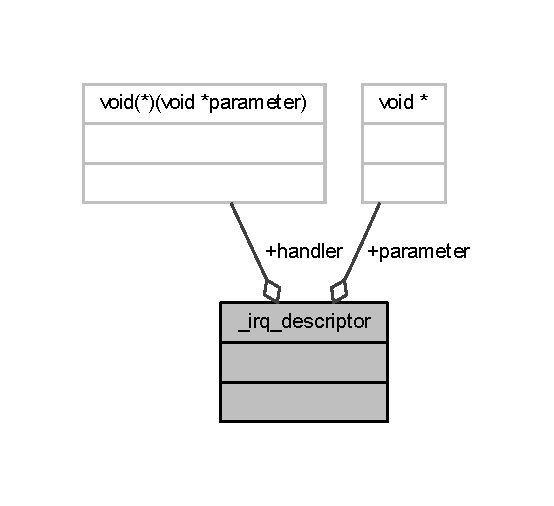
\includegraphics[width=266pt]{struct__irq__descriptor__coll__graph}
\end{center}
\end{figure}
\subsection*{Public Attributes}
\begin{DoxyCompactItemize}
\item 
void($\ast$ \hyperlink{struct__irq__descriptor_a5c5645efb32460ff3105eff8e6206b91}{handler} )(void $\ast$\hyperlink{struct__irq__descriptor_a9c58c3f373aebb6b725b9b47def981fd}{parameter})
\item 
void $\ast$ \hyperlink{struct__irq__descriptor_a9c58c3f373aebb6b725b9b47def981fd}{parameter}
\end{DoxyCompactItemize}


\subsection{Detailed Description}
I\+RQ descriptor. 

\subsection{Member Data Documentation}
\mbox{\Hypertarget{struct__irq__descriptor_a5c5645efb32460ff3105eff8e6206b91}\label{struct__irq__descriptor_a5c5645efb32460ff3105eff8e6206b91}} 
\index{\+\_\+irq\+\_\+descriptor@{\+\_\+irq\+\_\+descriptor}!handler@{handler}}
\index{handler@{handler}!\+\_\+irq\+\_\+descriptor@{\+\_\+irq\+\_\+descriptor}}
\subsubsection{\texorpdfstring{handler}{handler}}
{\footnotesize\ttfamily void($\ast$ \+\_\+irq\+\_\+descriptor\+::handler) (void $\ast$\hyperlink{struct__irq__descriptor_a9c58c3f373aebb6b725b9b47def981fd}{parameter})}

\mbox{\Hypertarget{struct__irq__descriptor_a9c58c3f373aebb6b725b9b47def981fd}\label{struct__irq__descriptor_a9c58c3f373aebb6b725b9b47def981fd}} 
\index{\+\_\+irq\+\_\+descriptor@{\+\_\+irq\+\_\+descriptor}!parameter@{parameter}}
\index{parameter@{parameter}!\+\_\+irq\+\_\+descriptor@{\+\_\+irq\+\_\+descriptor}}
\subsubsection{\texorpdfstring{parameter}{parameter}}
{\footnotesize\ttfamily void$\ast$ \+\_\+irq\+\_\+descriptor\+::parameter}



The documentation for this struct was generated from the following file\+:\begin{DoxyCompactItemize}
\item 
E\+:/\+Ha\+Ha\+Project/\+Atmel\+Xbee/\+A\+T\+Projects/\+Ha\+Ha/\+Ha\+Ha/hal/include/\hyperlink{hpl__irq_8h}{hpl\+\_\+irq.\+h}\end{DoxyCompactItemize}

\hypertarget{struct__usart__async__callbacks}{}\section{\+\_\+usart\+\_\+async\+\_\+callbacks Struct Reference}
\label{struct__usart__async__callbacks}\index{\+\_\+usart\+\_\+async\+\_\+callbacks@{\+\_\+usart\+\_\+async\+\_\+callbacks}}


U\+S\+A\+RT interrupt callbacks.  




{\ttfamily \#include $<$hpl\+\_\+usart\+\_\+async.\+h$>$}

\subsection*{Public Attributes}
\begin{DoxyCompactItemize}
\item 
\mbox{\Hypertarget{struct__usart__async__callbacks_a8213240efd24edc2266b1d499b42e945}\label{struct__usart__async__callbacks_a8213240efd24edc2266b1d499b42e945}} 
void($\ast$ {\bfseries tx\+\_\+byte\+\_\+sent} )(struct \hyperlink{struct__usart__async__device}{\+\_\+usart\+\_\+async\+\_\+device} $\ast$device)
\item 
\mbox{\Hypertarget{struct__usart__async__callbacks_af3670aee54cc400737048dde5c64d30e}\label{struct__usart__async__callbacks_af3670aee54cc400737048dde5c64d30e}} 
void($\ast$ {\bfseries rx\+\_\+done\+\_\+cb} )(struct \hyperlink{struct__usart__async__device}{\+\_\+usart\+\_\+async\+\_\+device} $\ast$device, uint8\+\_\+t data)
\item 
\mbox{\Hypertarget{struct__usart__async__callbacks_a71fe195e0159ee0b107df69b2b02f619}\label{struct__usart__async__callbacks_a71fe195e0159ee0b107df69b2b02f619}} 
void($\ast$ {\bfseries tx\+\_\+done\+\_\+cb} )(struct \hyperlink{struct__usart__async__device}{\+\_\+usart\+\_\+async\+\_\+device} $\ast$device)
\item 
\mbox{\Hypertarget{struct__usart__async__callbacks_a7b926fce0dbc8debda16675111ae754a}\label{struct__usart__async__callbacks_a7b926fce0dbc8debda16675111ae754a}} 
void($\ast$ {\bfseries error\+\_\+cb} )(struct \hyperlink{struct__usart__async__device}{\+\_\+usart\+\_\+async\+\_\+device} $\ast$device)
\end{DoxyCompactItemize}


\subsection{Detailed Description}
U\+S\+A\+RT interrupt callbacks. 

The documentation for this struct was generated from the following file\+:\begin{DoxyCompactItemize}
\item 
E\+:/\+Ha\+Ha\+Project/\+Atmel\+Xbee/\+A\+T\+Projects/\+Ha\+Ha/\+Ha\+Ha/hal/include/\hyperlink{hpl__usart__async_8h}{hpl\+\_\+usart\+\_\+async.\+h}\end{DoxyCompactItemize}

\hypertarget{struct__usart__async__device}{}\section{\+\_\+usart\+\_\+async\+\_\+device Struct Reference}
\label{struct__usart__async__device}\index{\+\_\+usart\+\_\+async\+\_\+device@{\+\_\+usart\+\_\+async\+\_\+device}}


U\+S\+A\+RT descriptor device structure.  




{\ttfamily \#include $<$hpl\+\_\+usart\+\_\+async.\+h$>$}



Collaboration diagram for \+\_\+usart\+\_\+async\+\_\+device\+:\nopagebreak
\begin{figure}[H]
\begin{center}
\leavevmode
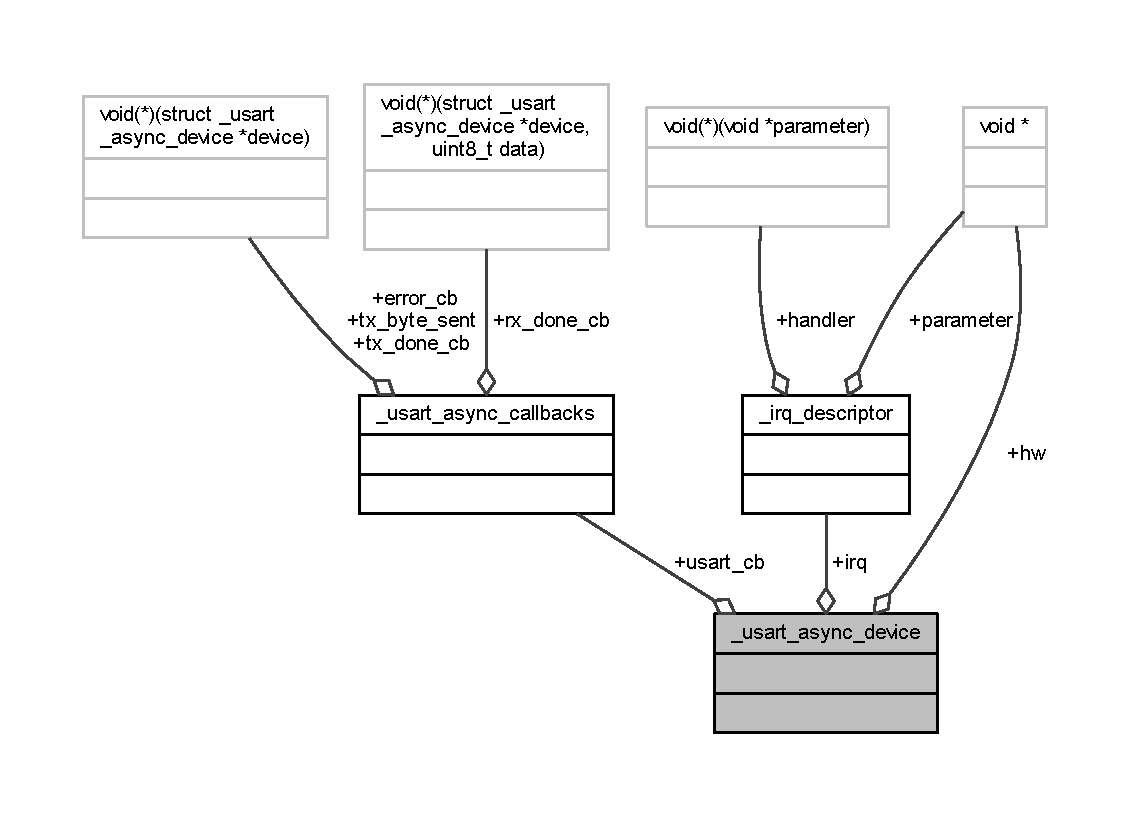
\includegraphics[width=350pt]{struct__usart__async__device__coll__graph}
\end{center}
\end{figure}
\subsection*{Public Attributes}
\begin{DoxyCompactItemize}
\item 
struct \hyperlink{struct__usart__async__callbacks}{\+\_\+usart\+\_\+async\+\_\+callbacks} \hyperlink{struct__usart__async__device_af36f1abd8113ed4a2f06a9084519f369}{usart\+\_\+cb}
\item 
struct \hyperlink{struct__irq__descriptor}{\+\_\+irq\+\_\+descriptor} \hyperlink{struct__usart__async__device_a0eb2cf8aa3661fe0a22168429c04bf57}{irq}
\item 
void $\ast$ \hyperlink{struct__usart__async__device_a3eae9af22755ddfe25f8406c2939262f}{hw}
\end{DoxyCompactItemize}


\subsection{Detailed Description}
U\+S\+A\+RT descriptor device structure. 

\subsection{Member Data Documentation}
\mbox{\Hypertarget{struct__usart__async__device_a3eae9af22755ddfe25f8406c2939262f}\label{struct__usart__async__device_a3eae9af22755ddfe25f8406c2939262f}} 
\index{\+\_\+usart\+\_\+async\+\_\+device@{\+\_\+usart\+\_\+async\+\_\+device}!hw@{hw}}
\index{hw@{hw}!\+\_\+usart\+\_\+async\+\_\+device@{\+\_\+usart\+\_\+async\+\_\+device}}
\subsubsection{\texorpdfstring{hw}{hw}}
{\footnotesize\ttfamily void$\ast$ \+\_\+usart\+\_\+async\+\_\+device\+::hw}

\mbox{\Hypertarget{struct__usart__async__device_a0eb2cf8aa3661fe0a22168429c04bf57}\label{struct__usart__async__device_a0eb2cf8aa3661fe0a22168429c04bf57}} 
\index{\+\_\+usart\+\_\+async\+\_\+device@{\+\_\+usart\+\_\+async\+\_\+device}!irq@{irq}}
\index{irq@{irq}!\+\_\+usart\+\_\+async\+\_\+device@{\+\_\+usart\+\_\+async\+\_\+device}}
\subsubsection{\texorpdfstring{irq}{irq}}
{\footnotesize\ttfamily struct \hyperlink{struct__irq__descriptor}{\+\_\+irq\+\_\+descriptor} \+\_\+usart\+\_\+async\+\_\+device\+::irq}

\mbox{\Hypertarget{struct__usart__async__device_af36f1abd8113ed4a2f06a9084519f369}\label{struct__usart__async__device_af36f1abd8113ed4a2f06a9084519f369}} 
\index{\+\_\+usart\+\_\+async\+\_\+device@{\+\_\+usart\+\_\+async\+\_\+device}!usart\+\_\+cb@{usart\+\_\+cb}}
\index{usart\+\_\+cb@{usart\+\_\+cb}!\+\_\+usart\+\_\+async\+\_\+device@{\+\_\+usart\+\_\+async\+\_\+device}}
\subsubsection{\texorpdfstring{usart\+\_\+cb}{usart\_cb}}
{\footnotesize\ttfamily struct \hyperlink{struct__usart__async__callbacks}{\+\_\+usart\+\_\+async\+\_\+callbacks} \+\_\+usart\+\_\+async\+\_\+device\+::usart\+\_\+cb}



The documentation for this struct was generated from the following file\+:\begin{DoxyCompactItemize}
\item 
E\+:/\+Ha\+Ha\+Project/\+Atmel\+Xbee/\+A\+T\+Projects/\+Ha\+Ha/\+Ha\+Ha/hal/include/\hyperlink{hpl__usart__async_8h}{hpl\+\_\+usart\+\_\+async.\+h}\end{DoxyCompactItemize}

\hypertarget{struct__usart__sync__device}{}\section{\+\_\+usart\+\_\+sync\+\_\+device Struct Reference}
\label{struct__usart__sync__device}\index{\+\_\+usart\+\_\+sync\+\_\+device@{\+\_\+usart\+\_\+sync\+\_\+device}}


U\+S\+A\+RT descriptor device structure.  




{\ttfamily \#include $<$hpl\+\_\+usart\+\_\+sync.\+h$>$}

\subsection*{Public Attributes}
\begin{DoxyCompactItemize}
\item 
\mbox{\Hypertarget{struct__usart__sync__device_a299ec1be7b3e3f53a8f8921823a3480c}\label{struct__usart__sync__device_a299ec1be7b3e3f53a8f8921823a3480c}} 
void $\ast$ {\bfseries hw}
\end{DoxyCompactItemize}


\subsection{Detailed Description}
U\+S\+A\+RT descriptor device structure. 

The documentation for this struct was generated from the following file\+:\begin{DoxyCompactItemize}
\item 
E\+:/\+Ha\+Ha\+Project/\+Atmel\+Xbee/\+A\+T\+Projects/\+Ha\+Ha/\+Ha\+Ha/hal/include/\hyperlink{hpl__usart__sync_8h}{hpl\+\_\+usart\+\_\+sync.\+h}\end{DoxyCompactItemize}

\hypertarget{structframe_r_x}{}\section{frame\+RX Struct Reference}
\label{structframe_r_x}\index{frame\+RX@{frame\+RX}}


{\ttfamily \#include $<$networkdevice.\+h$>$}



Collaboration diagram for frame\+RX\+:
\nopagebreak
\begin{figure}[H]
\begin{center}
\leavevmode
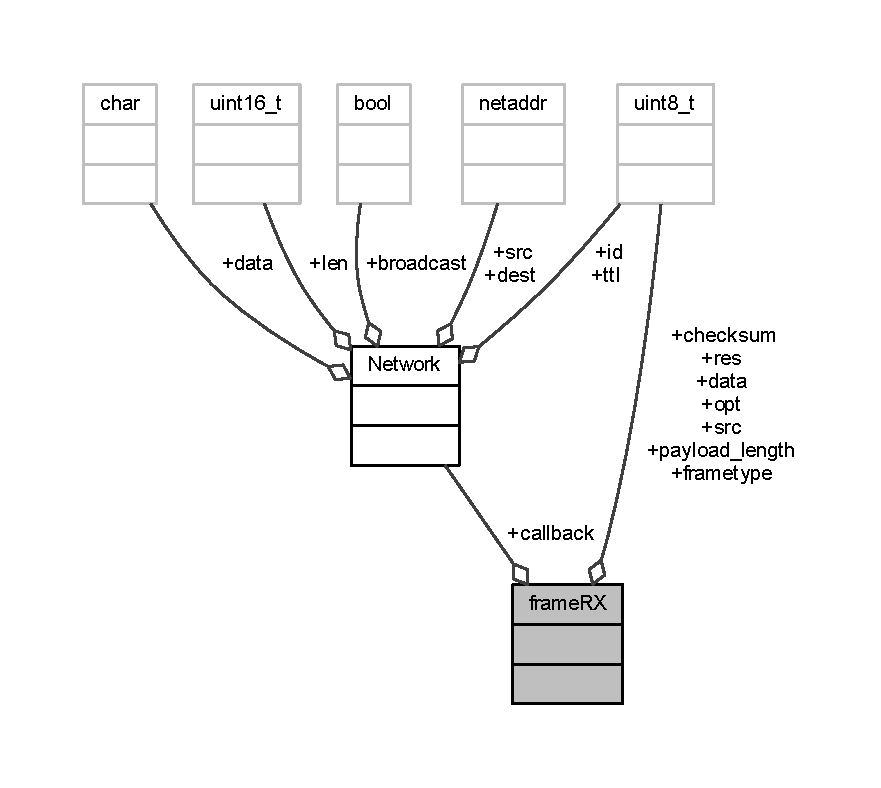
\includegraphics[width=240pt]{structframe_r_x__coll__graph}
\end{center}
\end{figure}
\subsection*{Public Attributes}
\begin{DoxyCompactItemize}
\item 
uint8\+\_\+t \hyperlink{structframe_r_x_a4684f3a419d7c6eaf5bded40cec73cdf}{frametype}
\item 
uint8\+\_\+t \hyperlink{structframe_r_x_a4a465dedf00b5d81f2f337c987b0ce96}{src} \mbox{[}8\mbox{]}
\item 
uint8\+\_\+t \hyperlink{structframe_r_x_a339160d2b3a24b3db0ea4318fc36227c}{res} \mbox{[}2\mbox{]}
\item 
uint8\+\_\+t \hyperlink{structframe_r_x_a46a068d1f1deb22e9e415b1ced537516}{opt}
\item 
uint8\+\_\+t \hyperlink{structframe_r_x_afdb061e4b3b406bf4890e95de2fbf474}{data} \mbox{[}100\mbox{]}
\item 
uint8\+\_\+t \hyperlink{structframe_r_x_a2ef590f48976b2550c7e12f2accf1e2f}{checksum}
\item 
uint8\+\_\+t \hyperlink{structframe_r_x_a8ffb1ad18c41d6943c8172042f965123}{payload\+\_\+length}
\item 
\hyperlink{networkdevice_8h_ad9c31236eed062640b6135a37fba175a}{xbee\+\_\+cb\+\_\+t} \hyperlink{structframe_r_x_a9483c0994c50cd55141215e73a75b95b}{callback}
\end{DoxyCompactItemize}


\subsection{Detailed Description}
\{ X\+Bee RX frame packet \} 

\subsection{Member Data Documentation}
\mbox{\Hypertarget{structframe_r_x_a9483c0994c50cd55141215e73a75b95b}\label{structframe_r_x_a9483c0994c50cd55141215e73a75b95b}} 
\index{frame\+RX@{frame\+RX}!callback@{callback}}
\index{callback@{callback}!frame\+RX@{frame\+RX}}
\subsubsection{\texorpdfstring{callback}{callback}}
{\footnotesize\ttfamily \hyperlink{networkdevice_8h_ad9c31236eed062640b6135a37fba175a}{xbee\+\_\+cb\+\_\+t} frame\+R\+X\+::callback}

\mbox{\Hypertarget{structframe_r_x_a2ef590f48976b2550c7e12f2accf1e2f}\label{structframe_r_x_a2ef590f48976b2550c7e12f2accf1e2f}} 
\index{frame\+RX@{frame\+RX}!checksum@{checksum}}
\index{checksum@{checksum}!frame\+RX@{frame\+RX}}
\subsubsection{\texorpdfstring{checksum}{checksum}}
{\footnotesize\ttfamily uint8\+\_\+t frame\+R\+X\+::checksum}

\mbox{\Hypertarget{structframe_r_x_afdb061e4b3b406bf4890e95de2fbf474}\label{structframe_r_x_afdb061e4b3b406bf4890e95de2fbf474}} 
\index{frame\+RX@{frame\+RX}!data@{data}}
\index{data@{data}!frame\+RX@{frame\+RX}}
\subsubsection{\texorpdfstring{data}{data}}
{\footnotesize\ttfamily uint8\+\_\+t frame\+R\+X\+::data\mbox{[}100\mbox{]}}

\mbox{\Hypertarget{structframe_r_x_a4684f3a419d7c6eaf5bded40cec73cdf}\label{structframe_r_x_a4684f3a419d7c6eaf5bded40cec73cdf}} 
\index{frame\+RX@{frame\+RX}!frametype@{frametype}}
\index{frametype@{frametype}!frame\+RX@{frame\+RX}}
\subsubsection{\texorpdfstring{frametype}{frametype}}
{\footnotesize\ttfamily uint8\+\_\+t frame\+R\+X\+::frametype}

\mbox{\Hypertarget{structframe_r_x_a46a068d1f1deb22e9e415b1ced537516}\label{structframe_r_x_a46a068d1f1deb22e9e415b1ced537516}} 
\index{frame\+RX@{frame\+RX}!opt@{opt}}
\index{opt@{opt}!frame\+RX@{frame\+RX}}
\subsubsection{\texorpdfstring{opt}{opt}}
{\footnotesize\ttfamily uint8\+\_\+t frame\+R\+X\+::opt}

\mbox{\Hypertarget{structframe_r_x_a8ffb1ad18c41d6943c8172042f965123}\label{structframe_r_x_a8ffb1ad18c41d6943c8172042f965123}} 
\index{frame\+RX@{frame\+RX}!payload\+\_\+length@{payload\+\_\+length}}
\index{payload\+\_\+length@{payload\+\_\+length}!frame\+RX@{frame\+RX}}
\subsubsection{\texorpdfstring{payload\+\_\+length}{payload\_length}}
{\footnotesize\ttfamily uint8\+\_\+t frame\+R\+X\+::payload\+\_\+length}

\mbox{\Hypertarget{structframe_r_x_a339160d2b3a24b3db0ea4318fc36227c}\label{structframe_r_x_a339160d2b3a24b3db0ea4318fc36227c}} 
\index{frame\+RX@{frame\+RX}!res@{res}}
\index{res@{res}!frame\+RX@{frame\+RX}}
\subsubsection{\texorpdfstring{res}{res}}
{\footnotesize\ttfamily uint8\+\_\+t frame\+R\+X\+::res\mbox{[}2\mbox{]}}

\mbox{\Hypertarget{structframe_r_x_a4a465dedf00b5d81f2f337c987b0ce96}\label{structframe_r_x_a4a465dedf00b5d81f2f337c987b0ce96}} 
\index{frame\+RX@{frame\+RX}!src@{src}}
\index{src@{src}!frame\+RX@{frame\+RX}}
\subsubsection{\texorpdfstring{src}{src}}
{\footnotesize\ttfamily uint8\+\_\+t frame\+R\+X\+::src\mbox{[}8\mbox{]}}



The documentation for this struct was generated from the following file\+:\begin{DoxyCompactItemize}
\item 
E\+:/\+Ha\+Ha\+Project/\+Atmel\+Xbee/\+A\+T\+Projects/\+Ha\+Ha/\+Ha\+Ha/networkdevice/\hyperlink{networkdevice_8h}{networkdevice.\+h}\end{DoxyCompactItemize}

\hypertarget{structframe_t_x}{}\section{frame\+TX Struct Reference}
\label{structframe_t_x}\index{frame\+TX@{frame\+TX}}
\subsection*{Public Attributes}
\begin{DoxyCompactItemize}
\item 
\mbox{\Hypertarget{structframe_t_x_ae0184264e132f9acfedd9d73e067d749}\label{structframe_t_x_ae0184264e132f9acfedd9d73e067d749}} 
uint8\+\_\+t {\bfseries frametype}
\item 
\mbox{\Hypertarget{structframe_t_x_a81728989f69fb448c3107efe57d9acee}\label{structframe_t_x_a81728989f69fb448c3107efe57d9acee}} 
uint8\+\_\+t {\bfseries frameid}
\item 
\mbox{\Hypertarget{structframe_t_x_ac6af0f89587bfdd91eabbc1664ed0b18}\label{structframe_t_x_ac6af0f89587bfdd91eabbc1664ed0b18}} 
uint8\+\_\+t {\bfseries dst} \mbox{[}8\mbox{]}
\item 
\mbox{\Hypertarget{structframe_t_x_aaa8e3f6c37ba7164586ece2aa05d02d1}\label{structframe_t_x_aaa8e3f6c37ba7164586ece2aa05d02d1}} 
uint8\+\_\+t {\bfseries res} \mbox{[}2\mbox{]}
\item 
\mbox{\Hypertarget{structframe_t_x_a9902ea07b8e5fc897038c4a78c052d46}\label{structframe_t_x_a9902ea07b8e5fc897038c4a78c052d46}} 
uint8\+\_\+t {\bfseries b\+\_\+rad}
\item 
\mbox{\Hypertarget{structframe_t_x_a683e80dc13eeb1ab084dcc79deea00a1}\label{structframe_t_x_a683e80dc13eeb1ab084dcc79deea00a1}} 
uint8\+\_\+t {\bfseries opt}
\item 
\mbox{\Hypertarget{structframe_t_x_a03427b6b3acbd35f51927438a3366cb5}\label{structframe_t_x_a03427b6b3acbd35f51927438a3366cb5}} 
char $\ast$ {\bfseries data}
\item 
\mbox{\Hypertarget{structframe_t_x_ae0f22f3d183e38466e30f42b9b69534e}\label{structframe_t_x_ae0f22f3d183e38466e30f42b9b69534e}} 
uint8\+\_\+t {\bfseries data\+\_\+len}
\end{DoxyCompactItemize}


The documentation for this struct was generated from the following file\+:\begin{DoxyCompactItemize}
\item 
E\+:/\+Ha\+Ha\+Project/\+Atmel-\/\+Xbee/\+A\+T\+Projects/\+Atmel\+\_\+\+Debug\+\_\+\+Xbee/\+Atmel\+\_\+\+Debug\+\_\+\+Xbee/xbee/xbee.\+c\end{DoxyCompactItemize}

\hypertarget{structio__descriptor}{}\section{io\+\_\+descriptor Struct Reference}
\label{structio__descriptor}\index{io\+\_\+descriptor@{io\+\_\+descriptor}}


I/O descriptor.  




{\ttfamily \#include $<$hal\+\_\+io.\+h$>$}



Collaboration diagram for io\+\_\+descriptor\+:\nopagebreak
\begin{figure}[H]
\begin{center}
\leavevmode
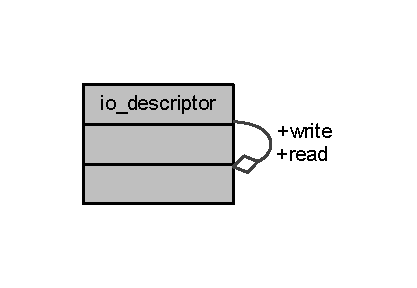
\includegraphics[width=200pt]{structio__descriptor__coll__graph}
\end{center}
\end{figure}
\subsection*{Public Attributes}
\begin{DoxyCompactItemize}
\item 
\hyperlink{group__doc__driver__hal__helper__io_gacb03c48993a6786f00946c196c40add1}{io\+\_\+write\+\_\+t} \hyperlink{structio__descriptor_a962235264b6c73e3ab712acb64022194}{write}
\item 
\hyperlink{group__doc__driver__hal__helper__io_ga4d9ae58de2887289fe09eac6f0aa8be7}{io\+\_\+read\+\_\+t} \hyperlink{structio__descriptor_a8ad97905c11dc07cd30373afc0fc146f}{read}
\end{DoxyCompactItemize}


\subsection{Detailed Description}
I/O descriptor. 

\subsection{Member Data Documentation}
\mbox{\Hypertarget{structio__descriptor_a8ad97905c11dc07cd30373afc0fc146f}\label{structio__descriptor_a8ad97905c11dc07cd30373afc0fc146f}} 
\index{io\+\_\+descriptor@{io\+\_\+descriptor}!read@{read}}
\index{read@{read}!io\+\_\+descriptor@{io\+\_\+descriptor}}
\subsubsection{\texorpdfstring{read}{read}}
{\footnotesize\ttfamily \hyperlink{group__doc__driver__hal__helper__io_ga4d9ae58de2887289fe09eac6f0aa8be7}{io\+\_\+read\+\_\+t} io\+\_\+descriptor\+::read}

The write function pointer. \mbox{\Hypertarget{structio__descriptor_a962235264b6c73e3ab712acb64022194}\label{structio__descriptor_a962235264b6c73e3ab712acb64022194}} 
\index{io\+\_\+descriptor@{io\+\_\+descriptor}!write@{write}}
\index{write@{write}!io\+\_\+descriptor@{io\+\_\+descriptor}}
\subsubsection{\texorpdfstring{write}{write}}
{\footnotesize\ttfamily \hyperlink{group__doc__driver__hal__helper__io_gacb03c48993a6786f00946c196c40add1}{io\+\_\+write\+\_\+t} io\+\_\+descriptor\+::write}



The documentation for this struct was generated from the following file\+:\begin{DoxyCompactItemize}
\item 
E\+:/\+Ha\+Ha\+Project/\+Atmel\+Xbee/\+A\+T\+Projects/\+Ha\+Ha/\+Ha\+Ha/hal/include/\hyperlink{hal__io_8h}{hal\+\_\+io.\+h}\end{DoxyCompactItemize}

\hypertarget{structlist__descriptor}{}\section{list\+\_\+descriptor Struct Reference}
\label{structlist__descriptor}\index{list\+\_\+descriptor@{list\+\_\+descriptor}}


List head type.  




{\ttfamily \#include $<$utils\+\_\+list.\+h$>$}



Collaboration diagram for list\+\_\+descriptor\+:\nopagebreak
\begin{figure}[H]
\begin{center}
\leavevmode
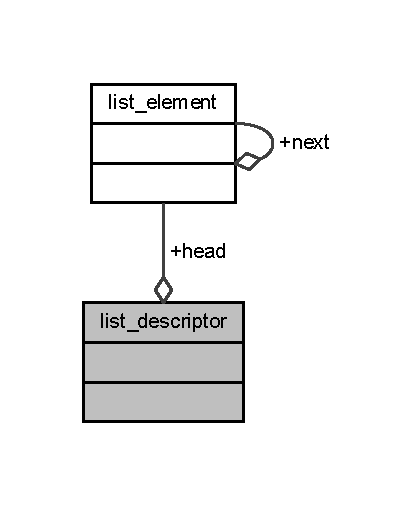
\includegraphics[width=199pt]{structlist__descriptor__coll__graph}
\end{center}
\end{figure}
\subsection*{Public Attributes}
\begin{DoxyCompactItemize}
\item 
struct \hyperlink{structlist__element}{list\+\_\+element} $\ast$ \hyperlink{structlist__descriptor_acc7a3bb5c92dc985a2a7c27c958f1ed8}{head}
\end{DoxyCompactItemize}


\subsection{Detailed Description}
List head type. 

\subsection{Member Data Documentation}
\mbox{\Hypertarget{structlist__descriptor_acc7a3bb5c92dc985a2a7c27c958f1ed8}\label{structlist__descriptor_acc7a3bb5c92dc985a2a7c27c958f1ed8}} 
\index{list\+\_\+descriptor@{list\+\_\+descriptor}!head@{head}}
\index{head@{head}!list\+\_\+descriptor@{list\+\_\+descriptor}}
\subsubsection{\texorpdfstring{head}{head}}
{\footnotesize\ttfamily struct \hyperlink{structlist__element}{list\+\_\+element}$\ast$ list\+\_\+descriptor\+::head}



The documentation for this struct was generated from the following file\+:\begin{DoxyCompactItemize}
\item 
E\+:/\+Ha\+Ha\+Project/\+Atmel\+Xbee/\+A\+T\+Projects/\+Ha\+Ha/\+Ha\+Ha/hal/utils/include/\hyperlink{utils__list_8h}{utils\+\_\+list.\+h}\end{DoxyCompactItemize}

\hypertarget{structlist__element}{}\section{list\+\_\+element Struct Reference}
\label{structlist__element}\index{list\+\_\+element@{list\+\_\+element}}


List element type.  




{\ttfamily \#include $<$utils\+\_\+list.\+h$>$}



Collaboration diagram for list\+\_\+element\+:
\nopagebreak
\begin{figure}[H]
\begin{center}
\leavevmode
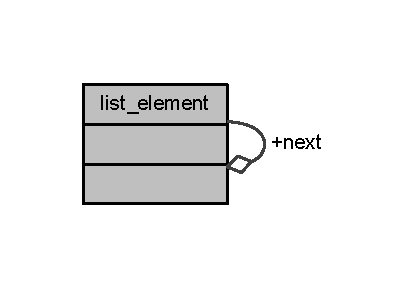
\includegraphics[width=195pt]{structlist__element__coll__graph}
\end{center}
\end{figure}
\subsection*{Public Attributes}
\begin{DoxyCompactItemize}
\item 
struct \hyperlink{structlist__element}{list\+\_\+element} $\ast$ \hyperlink{structlist__element_a66e1becb179745b2a4070941b9a4052d}{next}
\end{DoxyCompactItemize}


\subsection{Detailed Description}
List element type. 

\subsection{Member Data Documentation}
\mbox{\Hypertarget{structlist__element_a66e1becb179745b2a4070941b9a4052d}\label{structlist__element_a66e1becb179745b2a4070941b9a4052d}} 
\index{list\+\_\+element@{list\+\_\+element}!next@{next}}
\index{next@{next}!list\+\_\+element@{list\+\_\+element}}
\subsubsection{\texorpdfstring{next}{next}}
{\footnotesize\ttfamily struct \hyperlink{structlist__element}{list\+\_\+element}$\ast$ list\+\_\+element\+::next}



The documentation for this struct was generated from the following file\+:\begin{DoxyCompactItemize}
\item 
E\+:/\+Ha\+Ha\+Project/\+Atmel\+Xbee/\+A\+T\+Projects/\+Ha\+Ha/\+Ha\+Ha/hal/utils/include/\hyperlink{utils__list_8h}{utils\+\_\+list.\+h}\end{DoxyCompactItemize}

\hypertarget{struct_packet}{}\section{Packet Struct Reference}
\label{struct_packet}\index{Packet@{Packet}}
\subsection*{Public Attributes}
\begin{DoxyCompactItemize}
\item 
\mbox{\Hypertarget{struct_packet_add7e8d0db5c932cdf6ff0252697b88b0}\label{struct_packet_add7e8d0db5c932cdf6ff0252697b88b0}} 
opcode {\bfseries opcode}
\item 
\mbox{\Hypertarget{struct_packet_a06b33fa705a08bf26d8f15f4e5a5eacc}\label{struct_packet_a06b33fa705a08bf26d8f15f4e5a5eacc}} 
flags {\bfseries flags}
\item 
\mbox{\Hypertarget{struct_packet_abd4ca96c59b8446f7fb688c489e8b53f}\label{struct_packet_abd4ca96c59b8446f7fb688c489e8b53f}} 
char $\ast$ {\bfseries src}
\item 
\mbox{\Hypertarget{struct_packet_ac190cf6efc3180c1167886410748f1b9}\label{struct_packet_ac190cf6efc3180c1167886410748f1b9}} 
char $\ast$ {\bfseries dst}
\item 
\mbox{\Hypertarget{struct_packet_a6ce50b69127890b9012cb91f287f137f}\label{struct_packet_a6ce50b69127890b9012cb91f287f137f}} 
char $\ast$ {\bfseries data}
\end{DoxyCompactItemize}


The documentation for this struct was generated from the following file\+:\begin{DoxyCompactItemize}
\item 
E\+:/\+Ha\+Ha\+Project/\+Atmel\+Xbee/\+A\+T\+Projects/\+Ha\+Ha/\+Ha\+Ha/haha/network.\+h\end{DoxyCompactItemize}

\hypertarget{structringbuffer}{}\section{ringbuffer Struct Reference}
\label{structringbuffer}\index{ringbuffer@{ringbuffer}}


Ring buffer element type.  




{\ttfamily \#include $<$utils\+\_\+ringbuffer.\+h$>$}



Collaboration diagram for ringbuffer\+:
\nopagebreak
\begin{figure}[H]
\begin{center}
\leavevmode
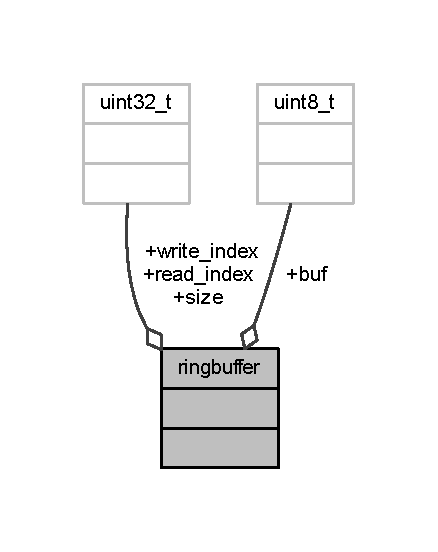
\includegraphics[width=210pt]{structringbuffer__coll__graph}
\end{center}
\end{figure}
\subsection*{Public Attributes}
\begin{DoxyCompactItemize}
\item 
uint8\+\_\+t $\ast$ \hyperlink{structringbuffer_a21e527bd1cee84a7b2c3d6d2da77584c}{buf}
\item 
uint32\+\_\+t \hyperlink{structringbuffer_a80a0c2fba71bab6481fe1a0bab9685ae}{size}
\item 
uint32\+\_\+t \hyperlink{structringbuffer_a1690488f3cc00713f660ab13ee18be5e}{read\+\_\+index}
\item 
uint32\+\_\+t \hyperlink{structringbuffer_a93936ef6a8e070e065448dbf49dcc93b}{write\+\_\+index}
\end{DoxyCompactItemize}


\subsection{Detailed Description}
Ring buffer element type. 

\subsection{Member Data Documentation}
\mbox{\Hypertarget{structringbuffer_a21e527bd1cee84a7b2c3d6d2da77584c}\label{structringbuffer_a21e527bd1cee84a7b2c3d6d2da77584c}} 
\index{ringbuffer@{ringbuffer}!buf@{buf}}
\index{buf@{buf}!ringbuffer@{ringbuffer}}
\subsubsection{\texorpdfstring{buf}{buf}}
{\footnotesize\ttfamily uint8\+\_\+t$\ast$ ringbuffer\+::buf}

\mbox{\Hypertarget{structringbuffer_a1690488f3cc00713f660ab13ee18be5e}\label{structringbuffer_a1690488f3cc00713f660ab13ee18be5e}} 
\index{ringbuffer@{ringbuffer}!read\+\_\+index@{read\+\_\+index}}
\index{read\+\_\+index@{read\+\_\+index}!ringbuffer@{ringbuffer}}
\subsubsection{\texorpdfstring{read\+\_\+index}{read\_index}}
{\footnotesize\ttfamily uint32\+\_\+t ringbuffer\+::read\+\_\+index}

\mbox{\Hypertarget{structringbuffer_a80a0c2fba71bab6481fe1a0bab9685ae}\label{structringbuffer_a80a0c2fba71bab6481fe1a0bab9685ae}} 
\index{ringbuffer@{ringbuffer}!size@{size}}
\index{size@{size}!ringbuffer@{ringbuffer}}
\subsubsection{\texorpdfstring{size}{size}}
{\footnotesize\ttfamily uint32\+\_\+t ringbuffer\+::size}

\mbox{\Hypertarget{structringbuffer_a93936ef6a8e070e065448dbf49dcc93b}\label{structringbuffer_a93936ef6a8e070e065448dbf49dcc93b}} 
\index{ringbuffer@{ringbuffer}!write\+\_\+index@{write\+\_\+index}}
\index{write\+\_\+index@{write\+\_\+index}!ringbuffer@{ringbuffer}}
\subsubsection{\texorpdfstring{write\+\_\+index}{write\_index}}
{\footnotesize\ttfamily uint32\+\_\+t ringbuffer\+::write\+\_\+index}



The documentation for this struct was generated from the following file\+:\begin{DoxyCompactItemize}
\item 
E\+:/\+Ha\+Ha\+Project/\+Atmel\+Xbee/\+A\+T\+Projects/\+Ha\+Ha/\+Ha\+Ha/hal/utils/include/\hyperlink{utils__ringbuffer_8h}{utils\+\_\+ringbuffer.\+h}\end{DoxyCompactItemize}

\hypertarget{structuart__config}{}\section{uart\+\_\+config Struct Reference}
\label{structuart__config}\index{uart\+\_\+config@{uart\+\_\+config}}


Configuration structure for the U\+A\+RT module.  




Collaboration diagram for uart\+\_\+config\+:
\nopagebreak
\begin{figure}[H]
\begin{center}
\leavevmode
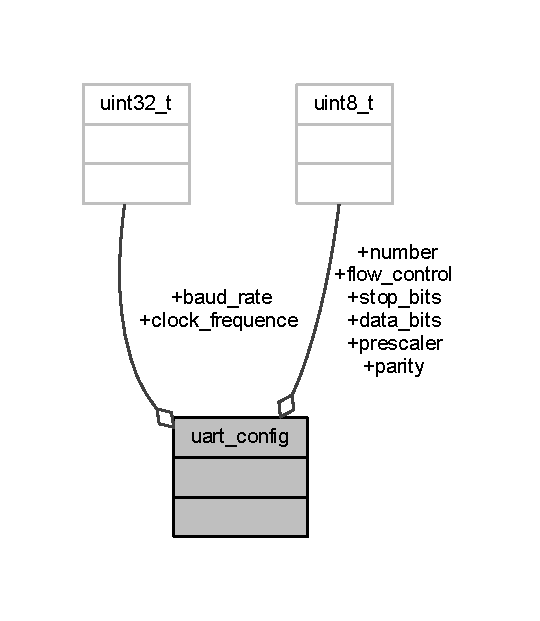
\includegraphics[width=259pt]{structuart__config__coll__graph}
\end{center}
\end{figure}
\subsection*{Public Attributes}
\begin{DoxyCompactItemize}
\item 
uint8\+\_\+t \hyperlink{structuart__config_a9f1c46bb7135a0a5dc0bce4f9982dc5f}{number}
\item 
uint32\+\_\+t \hyperlink{structuart__config_a3002fe5cb1c359f93dddb9198356bdcc}{baud\+\_\+rate}
\item 
uint8\+\_\+t \hyperlink{structuart__config_a93ee24cf6669fb4cfece78a53d3ec6c5}{data\+\_\+bits}
\item 
uint8\+\_\+t \hyperlink{structuart__config_a7b98cd63c531110dc3dc99e94db73642}{stop\+\_\+bits}
\item 
uint8\+\_\+t \hyperlink{structuart__config_a9371728729252797880de052aae01089}{parity}
\item 
uint8\+\_\+t \hyperlink{structuart__config_a30a786254694bfca26d7985545b6ffc6}{flow\+\_\+control}
\item 
uint8\+\_\+t \hyperlink{structuart__config_a9fb83c1cf1226b2dc4371bb79699dd71}{prescaler}
\item 
uint32\+\_\+t \hyperlink{structuart__config_a07d92658a8aea18961c39878c11fa689}{clock\+\_\+frequence}
\end{DoxyCompactItemize}


\subsection{Detailed Description}
Configuration structure for the U\+A\+RT module. 

This is the configuration structure for the U\+A\+RT Module in S\+A\+M\+B11. It is used as an argument for uart\+\_\+init to provide the desired configurations for the module. The structure should be initialized using the uart\+\_\+get\+\_\+config\+\_\+defaults . 

\subsection{Member Data Documentation}
\mbox{\Hypertarget{structuart__config_a3002fe5cb1c359f93dddb9198356bdcc}\label{structuart__config_a3002fe5cb1c359f93dddb9198356bdcc}} 
\index{uart\+\_\+config@{uart\+\_\+config}!baud\+\_\+rate@{baud\+\_\+rate}}
\index{baud\+\_\+rate@{baud\+\_\+rate}!uart\+\_\+config@{uart\+\_\+config}}
\subsubsection{\texorpdfstring{baud\+\_\+rate}{baud\_rate}}
{\footnotesize\ttfamily uint32\+\_\+t uart\+\_\+config\+::baud\+\_\+rate}

\mbox{\Hypertarget{structuart__config_a07d92658a8aea18961c39878c11fa689}\label{structuart__config_a07d92658a8aea18961c39878c11fa689}} 
\index{uart\+\_\+config@{uart\+\_\+config}!clock\+\_\+frequence@{clock\+\_\+frequence}}
\index{clock\+\_\+frequence@{clock\+\_\+frequence}!uart\+\_\+config@{uart\+\_\+config}}
\subsubsection{\texorpdfstring{clock\+\_\+frequence}{clock\_frequence}}
{\footnotesize\ttfamily uint32\+\_\+t uart\+\_\+config\+::clock\+\_\+frequence}

source clock frequency prescaler \mbox{\Hypertarget{structuart__config_a93ee24cf6669fb4cfece78a53d3ec6c5}\label{structuart__config_a93ee24cf6669fb4cfece78a53d3ec6c5}} 
\index{uart\+\_\+config@{uart\+\_\+config}!data\+\_\+bits@{data\+\_\+bits}}
\index{data\+\_\+bits@{data\+\_\+bits}!uart\+\_\+config@{uart\+\_\+config}}
\subsubsection{\texorpdfstring{data\+\_\+bits}{data\_bits}}
{\footnotesize\ttfamily uint8\+\_\+t uart\+\_\+config\+::data\+\_\+bits}

Baud rate \mbox{\Hypertarget{structuart__config_a30a786254694bfca26d7985545b6ffc6}\label{structuart__config_a30a786254694bfca26d7985545b6ffc6}} 
\index{uart\+\_\+config@{uart\+\_\+config}!flow\+\_\+control@{flow\+\_\+control}}
\index{flow\+\_\+control@{flow\+\_\+control}!uart\+\_\+config@{uart\+\_\+config}}
\subsubsection{\texorpdfstring{flow\+\_\+control}{flow\_control}}
{\footnotesize\ttfamily uint8\+\_\+t uart\+\_\+config\+::flow\+\_\+control}

Parity type \mbox{\Hypertarget{structuart__config_a9f1c46bb7135a0a5dc0bce4f9982dc5f}\label{structuart__config_a9f1c46bb7135a0a5dc0bce4f9982dc5f}} 
\index{uart\+\_\+config@{uart\+\_\+config}!number@{number}}
\index{number@{number}!uart\+\_\+config@{uart\+\_\+config}}
\subsubsection{\texorpdfstring{number}{number}}
{\footnotesize\ttfamily uint8\+\_\+t uart\+\_\+config\+::number}

\mbox{\Hypertarget{structuart__config_a9371728729252797880de052aae01089}\label{structuart__config_a9371728729252797880de052aae01089}} 
\index{uart\+\_\+config@{uart\+\_\+config}!parity@{parity}}
\index{parity@{parity}!uart\+\_\+config@{uart\+\_\+config}}
\subsubsection{\texorpdfstring{parity}{parity}}
{\footnotesize\ttfamily uint8\+\_\+t uart\+\_\+config\+::parity}

Number of stop bits \mbox{\Hypertarget{structuart__config_a9fb83c1cf1226b2dc4371bb79699dd71}\label{structuart__config_a9fb83c1cf1226b2dc4371bb79699dd71}} 
\index{uart\+\_\+config@{uart\+\_\+config}!prescaler@{prescaler}}
\index{prescaler@{prescaler}!uart\+\_\+config@{uart\+\_\+config}}
\subsubsection{\texorpdfstring{prescaler}{prescaler}}
{\footnotesize\ttfamily uint8\+\_\+t uart\+\_\+config\+::prescaler}

flow control type \mbox{\Hypertarget{structuart__config_a7b98cd63c531110dc3dc99e94db73642}\label{structuart__config_a7b98cd63c531110dc3dc99e94db73642}} 
\index{uart\+\_\+config@{uart\+\_\+config}!stop\+\_\+bits@{stop\+\_\+bits}}
\index{stop\+\_\+bits@{stop\+\_\+bits}!uart\+\_\+config@{uart\+\_\+config}}
\subsubsection{\texorpdfstring{stop\+\_\+bits}{stop\_bits}}
{\footnotesize\ttfamily uint8\+\_\+t uart\+\_\+config\+::stop\+\_\+bits}

Number of data bits 

The documentation for this struct was generated from the following file\+:\begin{DoxyCompactItemize}
\item 
E\+:/\+Ha\+Ha\+Project/\+Atmel\+Xbee/\+A\+T\+Projects/\+Ha\+Ha/\+Ha\+Ha/hpl/uart/\hyperlink{hpl__uart_8c}{hpl\+\_\+uart.\+c}\end{DoxyCompactItemize}

\hypertarget{structusart__async__callbacks}{}\section{usart\+\_\+async\+\_\+callbacks Struct Reference}
\label{structusart__async__callbacks}\index{usart\+\_\+async\+\_\+callbacks@{usart\+\_\+async\+\_\+callbacks}}


U\+S\+A\+RT callbacks.  




{\ttfamily \#include $<$hal\+\_\+usart\+\_\+async.\+h$>$}



Collaboration diagram for usart\+\_\+async\+\_\+callbacks\+:\nopagebreak
\begin{figure}[H]
\begin{center}
\leavevmode
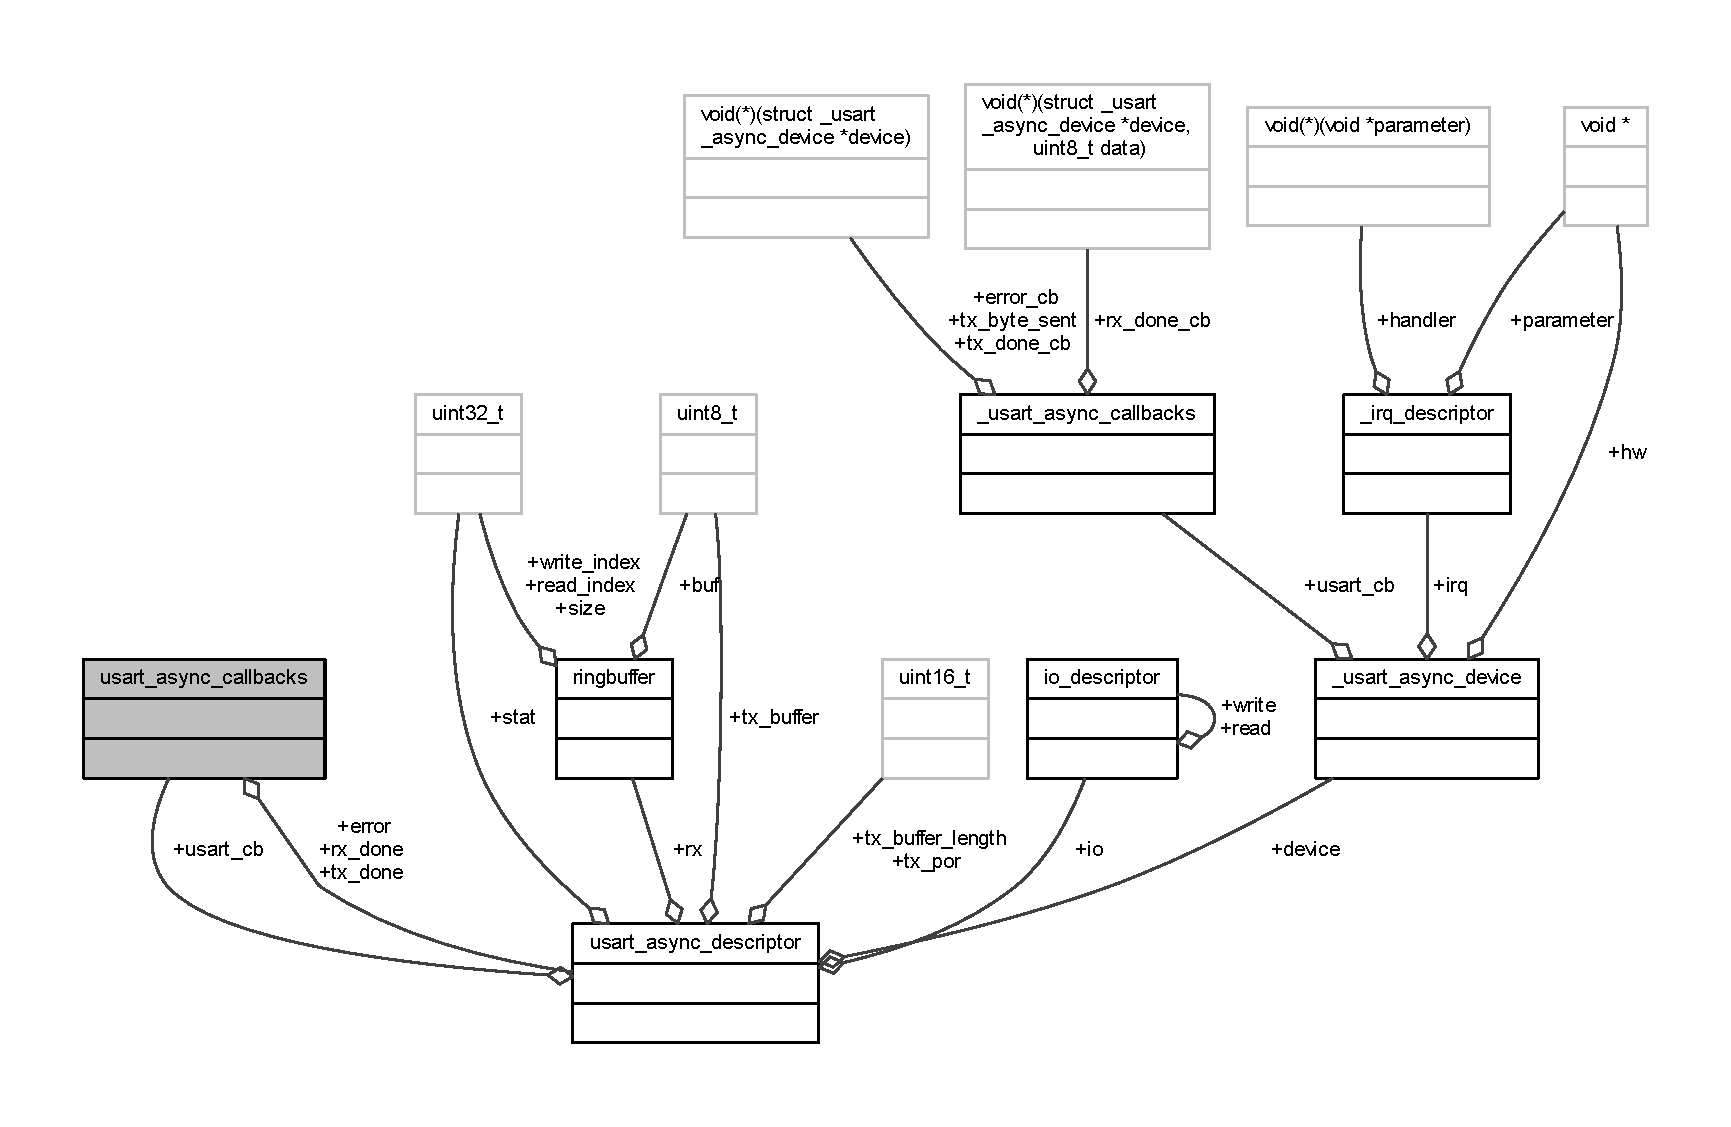
\includegraphics[width=350pt]{structusart__async__callbacks__coll__graph}
\end{center}
\end{figure}
\subsection*{Public Attributes}
\begin{DoxyCompactItemize}
\item 
\hyperlink{group__doc__driver__hal__usart__async_ga430e4080a53e1f39c4d46da01200f633}{usart\+\_\+cb\+\_\+t} \hyperlink{structusart__async__callbacks_a3b40d7b9783136ddf7e9bf49b9598d08}{tx\+\_\+done}
\item 
\hyperlink{group__doc__driver__hal__usart__async_ga430e4080a53e1f39c4d46da01200f633}{usart\+\_\+cb\+\_\+t} \hyperlink{structusart__async__callbacks_a5363ee6cc91c18b9cec22fcfc7270895}{rx\+\_\+done}
\item 
\hyperlink{group__doc__driver__hal__usart__async_ga430e4080a53e1f39c4d46da01200f633}{usart\+\_\+cb\+\_\+t} \hyperlink{structusart__async__callbacks_a04f0dca1ca10974d9458dd11871a5b58}{error}
\end{DoxyCompactItemize}


\subsection{Detailed Description}
U\+S\+A\+RT callbacks. 

\subsection{Member Data Documentation}
\mbox{\Hypertarget{structusart__async__callbacks_a04f0dca1ca10974d9458dd11871a5b58}\label{structusart__async__callbacks_a04f0dca1ca10974d9458dd11871a5b58}} 
\index{usart\+\_\+async\+\_\+callbacks@{usart\+\_\+async\+\_\+callbacks}!error@{error}}
\index{error@{error}!usart\+\_\+async\+\_\+callbacks@{usart\+\_\+async\+\_\+callbacks}}
\subsubsection{\texorpdfstring{error}{error}}
{\footnotesize\ttfamily \hyperlink{group__doc__driver__hal__usart__async_ga430e4080a53e1f39c4d46da01200f633}{usart\+\_\+cb\+\_\+t} usart\+\_\+async\+\_\+callbacks\+::error}

\mbox{\Hypertarget{structusart__async__callbacks_a5363ee6cc91c18b9cec22fcfc7270895}\label{structusart__async__callbacks_a5363ee6cc91c18b9cec22fcfc7270895}} 
\index{usart\+\_\+async\+\_\+callbacks@{usart\+\_\+async\+\_\+callbacks}!rx\+\_\+done@{rx\+\_\+done}}
\index{rx\+\_\+done@{rx\+\_\+done}!usart\+\_\+async\+\_\+callbacks@{usart\+\_\+async\+\_\+callbacks}}
\subsubsection{\texorpdfstring{rx\+\_\+done}{rx\_done}}
{\footnotesize\ttfamily \hyperlink{group__doc__driver__hal__usart__async_ga430e4080a53e1f39c4d46da01200f633}{usart\+\_\+cb\+\_\+t} usart\+\_\+async\+\_\+callbacks\+::rx\+\_\+done}

\mbox{\Hypertarget{structusart__async__callbacks_a3b40d7b9783136ddf7e9bf49b9598d08}\label{structusart__async__callbacks_a3b40d7b9783136ddf7e9bf49b9598d08}} 
\index{usart\+\_\+async\+\_\+callbacks@{usart\+\_\+async\+\_\+callbacks}!tx\+\_\+done@{tx\+\_\+done}}
\index{tx\+\_\+done@{tx\+\_\+done}!usart\+\_\+async\+\_\+callbacks@{usart\+\_\+async\+\_\+callbacks}}
\subsubsection{\texorpdfstring{tx\+\_\+done}{tx\_done}}
{\footnotesize\ttfamily \hyperlink{group__doc__driver__hal__usart__async_ga430e4080a53e1f39c4d46da01200f633}{usart\+\_\+cb\+\_\+t} usart\+\_\+async\+\_\+callbacks\+::tx\+\_\+done}



The documentation for this struct was generated from the following file\+:\begin{DoxyCompactItemize}
\item 
E\+:/\+Ha\+Ha\+Project/\+Atmel\+Xbee/\+A\+T\+Projects/\+Ha\+Ha/\+Ha\+Ha/hal/include/\hyperlink{hal__usart__async_8h}{hal\+\_\+usart\+\_\+async.\+h}\end{DoxyCompactItemize}

\hypertarget{structusart__async__descriptor}{}\section{usart\+\_\+async\+\_\+descriptor Struct Reference}
\label{structusart__async__descriptor}\index{usart\+\_\+async\+\_\+descriptor@{usart\+\_\+async\+\_\+descriptor}}


Asynchronous U\+S\+A\+RT descriptor structure.  




{\ttfamily \#include $<$hal\+\_\+usart\+\_\+async.\+h$>$}

\subsection*{Public Attributes}
\begin{DoxyCompactItemize}
\item 
\mbox{\Hypertarget{structusart__async__descriptor_a0b567a552bb9024872536444202911f3}\label{structusart__async__descriptor_a0b567a552bb9024872536444202911f3}} 
struct \hyperlink{structio__descriptor}{io\+\_\+descriptor} {\bfseries io}
\item 
\mbox{\Hypertarget{structusart__async__descriptor_a48ab054cada0897a439c0889ff769bbf}\label{structusart__async__descriptor_a48ab054cada0897a439c0889ff769bbf}} 
struct \hyperlink{struct__usart__async__device}{\+\_\+usart\+\_\+async\+\_\+device} {\bfseries device}
\item 
\mbox{\Hypertarget{structusart__async__descriptor_a84b19b1c19b845d0c2870ab306955b91}\label{structusart__async__descriptor_a84b19b1c19b845d0c2870ab306955b91}} 
struct \hyperlink{structusart__async__callbacks}{usart\+\_\+async\+\_\+callbacks} {\bfseries usart\+\_\+cb}
\item 
\mbox{\Hypertarget{structusart__async__descriptor_aa3b7aeba241416b7061e967d7832b203}\label{structusart__async__descriptor_aa3b7aeba241416b7061e967d7832b203}} 
uint32\+\_\+t {\bfseries stat}
\item 
\mbox{\Hypertarget{structusart__async__descriptor_a36cb240b43ed5ac70fb4b3cca1bcd071}\label{structusart__async__descriptor_a36cb240b43ed5ac70fb4b3cca1bcd071}} 
struct \hyperlink{structringbuffer}{ringbuffer} {\bfseries rx}
\item 
\mbox{\Hypertarget{structusart__async__descriptor_aecbbb71691ffede25d2ec628947a4305}\label{structusart__async__descriptor_aecbbb71691ffede25d2ec628947a4305}} 
uint16\+\_\+t {\bfseries tx\+\_\+por}
\item 
\mbox{\Hypertarget{structusart__async__descriptor_a9ed199abede0cb07c2b91aeb443d3ada}\label{structusart__async__descriptor_a9ed199abede0cb07c2b91aeb443d3ada}} 
uint8\+\_\+t $\ast$ {\bfseries tx\+\_\+buffer}
\item 
\mbox{\Hypertarget{structusart__async__descriptor_a0a4c5301c869bb18cb57deb866707e66}\label{structusart__async__descriptor_a0a4c5301c869bb18cb57deb866707e66}} 
uint16\+\_\+t {\bfseries tx\+\_\+buffer\+\_\+length}
\end{DoxyCompactItemize}


\subsection{Detailed Description}
Asynchronous U\+S\+A\+RT descriptor structure. 

The documentation for this struct was generated from the following file\+:\begin{DoxyCompactItemize}
\item 
E\+:/\+Ha\+Ha\+Project/\+Atmel\+Xbee/\+A\+T\+Projects/\+Ha\+Ha/\+Ha\+Ha/hal/include/\hyperlink{hal__usart__async_8h}{hal\+\_\+usart\+\_\+async.\+h}\end{DoxyCompactItemize}

\hypertarget{structusart__async__status}{}\section{usart\+\_\+async\+\_\+status Struct Reference}
\label{structusart__async__status}\index{usart\+\_\+async\+\_\+status@{usart\+\_\+async\+\_\+status}}


U\+S\+A\+RT status Status descriptor holds the current status of transfer.  




{\ttfamily \#include $<$hal\+\_\+usart\+\_\+async.\+h$>$}

\subsection*{Public Attributes}
\begin{DoxyCompactItemize}
\item 
uint32\+\_\+t \hyperlink{structusart__async__status_a6d85ac04ed76a86bb9c49bb45a848d9a}{flags}
\item 
uint16\+\_\+t \hyperlink{structusart__async__status_a5680433094528c4ff7bcd49fba77e970}{txcnt}
\item 
uint16\+\_\+t \hyperlink{structusart__async__status_ac32698399322fed11e6914cbd88f5ee5}{rxcnt}
\end{DoxyCompactItemize}


\subsection{Detailed Description}
U\+S\+A\+RT status Status descriptor holds the current status of transfer. 

\subsection{Member Data Documentation}
\mbox{\Hypertarget{structusart__async__status_a6d85ac04ed76a86bb9c49bb45a848d9a}\label{structusart__async__status_a6d85ac04ed76a86bb9c49bb45a848d9a}} 
\index{usart\+\_\+async\+\_\+status@{usart\+\_\+async\+\_\+status}!flags@{flags}}
\index{flags@{flags}!usart\+\_\+async\+\_\+status@{usart\+\_\+async\+\_\+status}}
\subsubsection{\texorpdfstring{flags}{flags}}
{\footnotesize\ttfamily uint32\+\_\+t usart\+\_\+async\+\_\+status\+::flags}

Status flags \mbox{\Hypertarget{structusart__async__status_ac32698399322fed11e6914cbd88f5ee5}\label{structusart__async__status_ac32698399322fed11e6914cbd88f5ee5}} 
\index{usart\+\_\+async\+\_\+status@{usart\+\_\+async\+\_\+status}!rxcnt@{rxcnt}}
\index{rxcnt@{rxcnt}!usart\+\_\+async\+\_\+status@{usart\+\_\+async\+\_\+status}}
\subsubsection{\texorpdfstring{rxcnt}{rxcnt}}
{\footnotesize\ttfamily uint16\+\_\+t usart\+\_\+async\+\_\+status\+::rxcnt}

Number of characters receviced \mbox{\Hypertarget{structusart__async__status_a5680433094528c4ff7bcd49fba77e970}\label{structusart__async__status_a5680433094528c4ff7bcd49fba77e970}} 
\index{usart\+\_\+async\+\_\+status@{usart\+\_\+async\+\_\+status}!txcnt@{txcnt}}
\index{txcnt@{txcnt}!usart\+\_\+async\+\_\+status@{usart\+\_\+async\+\_\+status}}
\subsubsection{\texorpdfstring{txcnt}{txcnt}}
{\footnotesize\ttfamily uint16\+\_\+t usart\+\_\+async\+\_\+status\+::txcnt}

Number of characters transmitted 

The documentation for this struct was generated from the following file\+:\begin{DoxyCompactItemize}
\item 
E\+:/\+Ha\+Ha\+Project/\+Atmel\+Xbee/\+A\+T\+Projects/\+Ha\+Ha/\+Ha\+Ha/hal/include/\hyperlink{hal__usart__async_8h}{hal\+\_\+usart\+\_\+async.\+h}\end{DoxyCompactItemize}

\hypertarget{unionusart__flow__control__state}{}\section{usart\+\_\+flow\+\_\+control\+\_\+state Union Reference}
\label{unionusart__flow__control__state}\index{usart\+\_\+flow\+\_\+control\+\_\+state@{usart\+\_\+flow\+\_\+control\+\_\+state}}


U\+S\+A\+RT flow control state.  




{\ttfamily \#include $<$hpl\+\_\+usart.\+h$>$}

\subsection*{Public Attributes}
\begin{DoxyCompactItemize}
\item 
\mbox{\Hypertarget{unionusart__flow__control__state_a6ade7bab5cb48566816f4e6d6c429839}\label{unionusart__flow__control__state_a6ade7bab5cb48566816f4e6d6c429839}} 
\begin{tabbing}
xx\=xx\=xx\=xx\=xx\=xx\=xx\=xx\=xx\=\kill
struct \{\\
\>uint8\_t {\bfseries cts}: 1\\
\>uint8\_t {\bfseries rts}: 1\\
\>uint8\_t {\bfseries unavailable}: 1\\
\>uint8\_t {\bfseries reserved}: 5\\
\} {\bfseries bit}\\

\end{tabbing}\item 
\mbox{\Hypertarget{unionusart__flow__control__state_a89fd17179ea28972111f4e5822de3e4e}\label{unionusart__flow__control__state_a89fd17179ea28972111f4e5822de3e4e}} 
uint8\+\_\+t {\bfseries value}
\end{DoxyCompactItemize}


\subsection{Detailed Description}
U\+S\+A\+RT flow control state. 

The documentation for this union was generated from the following file\+:\begin{DoxyCompactItemize}
\item 
E\+:/\+Ha\+Ha\+Project/\+Atmel\+Xbee/\+A\+T\+Projects/\+Ha\+Ha/\+Ha\+Ha/hal/include/\hyperlink{hpl__usart_8h}{hpl\+\_\+usart.\+h}\end{DoxyCompactItemize}

\hypertarget{structusart__sync__descriptor}{}\section{usart\+\_\+sync\+\_\+descriptor Struct Reference}
\label{structusart__sync__descriptor}\index{usart\+\_\+sync\+\_\+descriptor@{usart\+\_\+sync\+\_\+descriptor}}


Synchronous U\+S\+A\+RT descriptor.  




{\ttfamily \#include $<$hal\+\_\+usart\+\_\+sync.\+h$>$}



Collaboration diagram for usart\+\_\+sync\+\_\+descriptor\+:\nopagebreak
\begin{figure}[H]
\begin{center}
\leavevmode
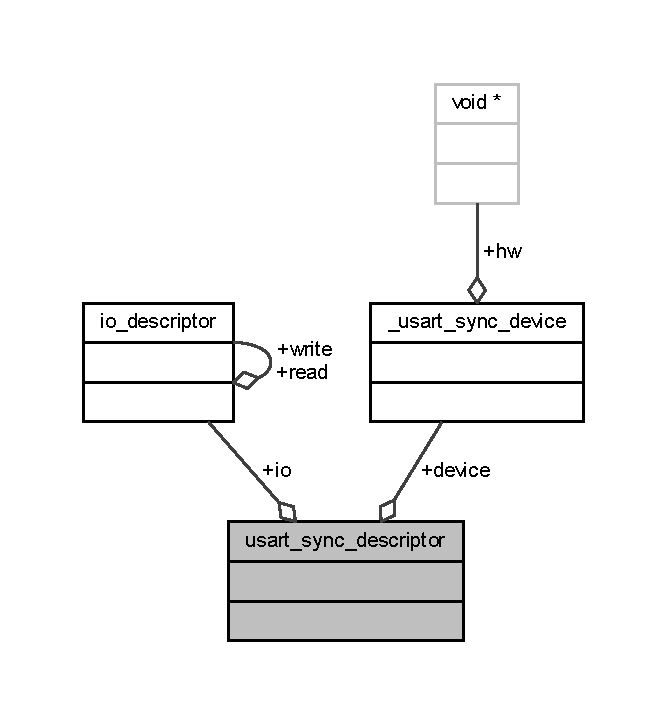
\includegraphics[width=320pt]{structusart__sync__descriptor__coll__graph}
\end{center}
\end{figure}
\subsection*{Public Attributes}
\begin{DoxyCompactItemize}
\item 
struct \hyperlink{structio__descriptor}{io\+\_\+descriptor} \hyperlink{structusart__sync__descriptor_a9ef5dd1d1c2010fc961d3e803c7429cb}{io}
\item 
struct \hyperlink{struct__usart__sync__device}{\+\_\+usart\+\_\+sync\+\_\+device} \hyperlink{structusart__sync__descriptor_a825cfcdd7f23413952a2a198b8a07ad5}{device}
\end{DoxyCompactItemize}


\subsection{Detailed Description}
Synchronous U\+S\+A\+RT descriptor. 

\subsection{Member Data Documentation}
\mbox{\Hypertarget{structusart__sync__descriptor_a825cfcdd7f23413952a2a198b8a07ad5}\label{structusart__sync__descriptor_a825cfcdd7f23413952a2a198b8a07ad5}} 
\index{usart\+\_\+sync\+\_\+descriptor@{usart\+\_\+sync\+\_\+descriptor}!device@{device}}
\index{device@{device}!usart\+\_\+sync\+\_\+descriptor@{usart\+\_\+sync\+\_\+descriptor}}
\subsubsection{\texorpdfstring{device}{device}}
{\footnotesize\ttfamily struct \hyperlink{struct__usart__sync__device}{\+\_\+usart\+\_\+sync\+\_\+device} usart\+\_\+sync\+\_\+descriptor\+::device}

\mbox{\Hypertarget{structusart__sync__descriptor_a9ef5dd1d1c2010fc961d3e803c7429cb}\label{structusart__sync__descriptor_a9ef5dd1d1c2010fc961d3e803c7429cb}} 
\index{usart\+\_\+sync\+\_\+descriptor@{usart\+\_\+sync\+\_\+descriptor}!io@{io}}
\index{io@{io}!usart\+\_\+sync\+\_\+descriptor@{usart\+\_\+sync\+\_\+descriptor}}
\subsubsection{\texorpdfstring{io}{io}}
{\footnotesize\ttfamily struct \hyperlink{structio__descriptor}{io\+\_\+descriptor} usart\+\_\+sync\+\_\+descriptor\+::io}



The documentation for this struct was generated from the following file\+:\begin{DoxyCompactItemize}
\item 
E\+:/\+Ha\+Ha\+Project/\+Atmel\+Xbee/\+A\+T\+Projects/\+Ha\+Ha/\+Ha\+Ha/hal/include/\hyperlink{hal__usart__sync_8h}{hal\+\_\+usart\+\_\+sync.\+h}\end{DoxyCompactItemize}

\chapter{File Documentation}
\hypertarget{_r_t_e___components_8h}{}\section{E\+:/\+Ha\+Ha\+Project/\+Atmel\+Xbee/\+A\+T\+Projects/\+Ha\+Ha/\+Ha\+Ha/\+Config/\+R\+T\+E\+\_\+\+Components.h File Reference}
\label{_r_t_e___components_8h}\index{E\+:/\+Ha\+Ha\+Project/\+Atmel\+Xbee/\+A\+T\+Projects/\+Ha\+Ha/\+Ha\+Ha/\+Config/\+R\+T\+E\+\_\+\+Components.\+h@{E\+:/\+Ha\+Ha\+Project/\+Atmel\+Xbee/\+A\+T\+Projects/\+Ha\+Ha/\+Ha\+Ha/\+Config/\+R\+T\+E\+\_\+\+Components.\+h}}


Autogenerated A\+PI include file for the Atmel Configuration Management Engine (A\+C\+ME)  




\subsection{Detailed Description}
Autogenerated A\+PI include file for the Atmel Configuration Management Engine (A\+C\+ME) 

Copyright (c) 2012 Atmel Corporation. All rights reserved.
\hypertarget{startup__samb11_8c}{}\section{E\+:/\+Ha\+Ha\+Project/\+Atmel\+Xbee/\+A\+T\+Projects/\+Ha\+Ha/\+Ha\+Ha/\+Device\+\_\+\+Startup/startup\+\_\+samb11.c File Reference}
\label{startup__samb11_8c}\index{E\+:/\+Ha\+Ha\+Project/\+Atmel\+Xbee/\+A\+T\+Projects/\+Ha\+Ha/\+Ha\+Ha/\+Device\+\_\+\+Startup/startup\+\_\+samb11.\+c@{E\+:/\+Ha\+Ha\+Project/\+Atmel\+Xbee/\+A\+T\+Projects/\+Ha\+Ha/\+Ha\+Ha/\+Device\+\_\+\+Startup/startup\+\_\+samb11.\+c}}


G\+CC entry point for S\+A\+M\+B11 projects. To be scheduled to run as a task in the B\+LE OS.  


{\ttfamily \#include \char`\"{}sam.\+h\char`\"{}}\newline
\subsection*{Functions}
\begin{DoxyCompactItemize}
\item 
\mbox{\Hypertarget{startup__samb11_8c_a840291bc02cba5474a4cb46a9b9566fe}\label{startup__samb11_8c_a840291bc02cba5474a4cb46a9b9566fe}} 
int \hyperlink{startup__samb11_8c_a840291bc02cba5474a4cb46a9b9566fe}{main} (void)
\begin{DoxyCompactList}\small\item\em This is the code that gets called on processor reset. To initialize the device, and call the \hyperlink{startup__samb11_8c_a840291bc02cba5474a4cb46a9b9566fe}{main()} routine. \end{DoxyCompactList}\item 
\mbox{\Hypertarget{startup__samb11_8c_a5f388c8556f7cb6a84b5692db6b6ad80}\label{startup__samb11_8c_a5f388c8556f7cb6a84b5692db6b6ad80}} 
void {\bfseries \+\_\+\+\_\+libc\+\_\+init\+\_\+array} (void)
\item 
\mbox{\Hypertarget{startup__samb11_8c_acce9c970b367ddeb57c853b26cff3d84}\label{startup__samb11_8c_acce9c970b367ddeb57c853b26cff3d84}} 
void {\bfseries app\+\_\+entry} (void)
\end{DoxyCompactItemize}
\subsection*{Variables}
\begin{DoxyCompactItemize}
\item 
\mbox{\Hypertarget{startup__samb11_8c_abba93927cdaa2d32967cfc724f47cf8f}\label{startup__samb11_8c_abba93927cdaa2d32967cfc724f47cf8f}} 
uint32\+\_\+t {\bfseries \+\_\+etext}
\item 
\mbox{\Hypertarget{startup__samb11_8c_ac50d147d186c5fcf7efa97a4197e530e}\label{startup__samb11_8c_ac50d147d186c5fcf7efa97a4197e530e}} 
uint32\+\_\+t {\bfseries \+\_\+srelocate}
\item 
\mbox{\Hypertarget{startup__samb11_8c_a59f8a39545ac1b9b88d4228c40c910b9}\label{startup__samb11_8c_a59f8a39545ac1b9b88d4228c40c910b9}} 
uint32\+\_\+t {\bfseries \+\_\+erelocate}
\item 
\mbox{\Hypertarget{startup__samb11_8c_a5c6ed4fbf19b32595d4afb2c25aa8363}\label{startup__samb11_8c_a5c6ed4fbf19b32595d4afb2c25aa8363}} 
uint32\+\_\+t {\bfseries \+\_\+szero}
\item 
\mbox{\Hypertarget{startup__samb11_8c_ad4c54e57daaa1859c4fd4208ed7d31fa}\label{startup__samb11_8c_ad4c54e57daaa1859c4fd4208ed7d31fa}} 
uint32\+\_\+t {\bfseries \+\_\+ezero}
\end{DoxyCompactItemize}


\subsection{Detailed Description}
G\+CC entry point for S\+A\+M\+B11 projects. To be scheduled to run as a task in the B\+LE OS. 

Copyright (c) 2014 Atmel Corporation. All rights reserved.
\hypertarget{system__samb11_8c}{}\section{E\+:/\+Ha\+Ha\+Project/\+Atmel\+Xbee/\+A\+T\+Projects/\+Ha\+Ha/\+Ha\+Ha/\+Device\+\_\+\+Startup/system\+\_\+samb11.c File Reference}
\label{system__samb11_8c}\index{E\+:/\+Ha\+Ha\+Project/\+Atmel\+Xbee/\+A\+T\+Projects/\+Ha\+Ha/\+Ha\+Ha/\+Device\+\_\+\+Startup/system\+\_\+samb11.\+c@{E\+:/\+Ha\+Ha\+Project/\+Atmel\+Xbee/\+A\+T\+Projects/\+Ha\+Ha/\+Ha\+Ha/\+Device\+\_\+\+Startup/system\+\_\+samb11.\+c}}


Low-\/level initialization functions called upon chip startup.  


{\ttfamily \#include \char`\"{}sam.\+h\char`\"{}}\newline
Include dependency graph for system\+\_\+samb11.\+c\+:\nopagebreak
\begin{figure}[H]
\begin{center}
\leavevmode
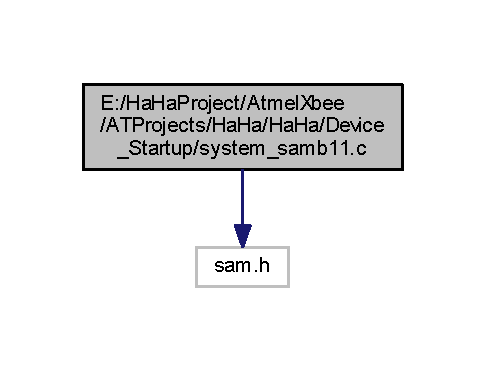
\includegraphics[width=233pt]{system__samb11_8c__incl}
\end{center}
\end{figure}


\subsection{Detailed Description}
Low-\/level initialization functions called upon chip startup. 

Copyright (c) 2015 Atmel Corporation. All rights reserved.
\hypertarget{haha_utils_8h}{}\section{E\+:/\+Ha\+Ha\+Project/\+Atmel\+Xbee/\+A\+T\+Projects/\+Ha\+Ha/\+Ha\+Ha/devstuff/haha\+Utils.h File Reference}
\label{haha_utils_8h}\index{E\+:/\+Ha\+Ha\+Project/\+Atmel\+Xbee/\+A\+T\+Projects/\+Ha\+Ha/\+Ha\+Ha/devstuff/haha\+Utils.\+h@{E\+:/\+Ha\+Ha\+Project/\+Atmel\+Xbee/\+A\+T\+Projects/\+Ha\+Ha/\+Ha\+Ha/devstuff/haha\+Utils.\+h}}


Utility functions/variables and debug functionality.  


{\ttfamily \#include $<$ctype.\+h$>$}\newline
{\ttfamily \#include $<$stdio.\+h$>$}\newline
{\ttfamily \#include $<$stdio\+\_\+start.\+h$>$}\newline
\subsection*{Macros}
\begin{DoxyCompactItemize}
\item 
\mbox{\Hypertarget{haha_utils_8h_abb452686968e48b67397da5f97445f5b}\label{haha_utils_8h_abb452686968e48b67397da5f97445f5b}} 
\#define {\bfseries bool}~uint8\+\_\+t
\item 
\mbox{\Hypertarget{haha_utils_8h_aa8cecfc5c5c054d2875c03e77b7be15d}\label{haha_utils_8h_aa8cecfc5c5c054d2875c03e77b7be15d}} 
\#define {\bfseries T\+R\+UE}~1
\item 
\mbox{\Hypertarget{haha_utils_8h_aa93f0eb578d23995850d61f7d61c55c1}\label{haha_utils_8h_aa93f0eb578d23995850d61f7d61c55c1}} 
\#define {\bfseries F\+A\+L\+SE}~0
\item 
\#define \hyperlink{haha_utils_8h_ad5aeca1a1a793c8ba18f85cbac89e768}{D\+E\+B\+U\+G\+\_\+\+P\+R\+I\+NT}~1
\item 
\mbox{\Hypertarget{haha_utils_8h_a185c556500093ce1d9b97379ab00449f}\label{haha_utils_8h_a185c556500093ce1d9b97379ab00449f}} 
\#define {\bfseries H\+A\+H\+A\+D\+E\+B\+UG}(format,  args...)~printf(format, \#\# args)
\end{DoxyCompactItemize}
\subsection*{Functions}
\begin{DoxyCompactItemize}
\item 
void \hyperlink{haha_utils_8h_a7f2dfce1046bdd2a2b753643726c2346}{delay} (uint32\+\_\+t ms)
\begin{DoxyCompactList}\small\item\em \{ Delays execution in ms \} \end{DoxyCompactList}\item 
void \hyperlink{haha_utils_8h_ada9e8340bd19f1dd65b4862295e6b0a3}{print\+Buff} (char $\ast$data, uint8\+\_\+t len, char $\ast$specifier)
\begin{DoxyCompactList}\small\item\em \{ Print a buffer to stdout \} \end{DoxyCompactList}\item 
uint8\+\_\+t \hyperlink{haha_utils_8h_aa74dea5951b0fe8a0afab70b3c83cbb3}{asciihex\+\_\+to\+\_\+byte} (uint8\+\_\+t d1, uint8\+\_\+t d2)
\begin{DoxyCompactList}\small\item\em \{ Takes two char and converts to Hex \} \end{DoxyCompactList}\end{DoxyCompactItemize}


\subsection{Detailed Description}
Utility functions/variables and debug functionality. 



\subsection{Macro Definition Documentation}
\mbox{\Hypertarget{haha_utils_8h_ad5aeca1a1a793c8ba18f85cbac89e768}\label{haha_utils_8h_ad5aeca1a1a793c8ba18f85cbac89e768}} 
\index{haha\+Utils.\+h@{haha\+Utils.\+h}!D\+E\+B\+U\+G\+\_\+\+P\+R\+I\+NT@{D\+E\+B\+U\+G\+\_\+\+P\+R\+I\+NT}}
\index{D\+E\+B\+U\+G\+\_\+\+P\+R\+I\+NT@{D\+E\+B\+U\+G\+\_\+\+P\+R\+I\+NT}!haha\+Utils.\+h@{haha\+Utils.\+h}}
\subsubsection{\texorpdfstring{D\+E\+B\+U\+G\+\_\+\+P\+R\+I\+NT}{DEBUG\_PRINT}}
{\footnotesize\ttfamily \#define D\+E\+B\+U\+G\+\_\+\+P\+R\+I\+NT~1}

\{ \#define for debug printing \} 

\subsection{Function Documentation}
\mbox{\Hypertarget{haha_utils_8h_aa74dea5951b0fe8a0afab70b3c83cbb3}\label{haha_utils_8h_aa74dea5951b0fe8a0afab70b3c83cbb3}} 
\index{haha\+Utils.\+h@{haha\+Utils.\+h}!asciihex\+\_\+to\+\_\+byte@{asciihex\+\_\+to\+\_\+byte}}
\index{asciihex\+\_\+to\+\_\+byte@{asciihex\+\_\+to\+\_\+byte}!haha\+Utils.\+h@{haha\+Utils.\+h}}
\subsubsection{\texorpdfstring{asciihex\+\_\+to\+\_\+byte()}{asciihex\_to\_byte()}}
{\footnotesize\ttfamily uint8\+\_\+t asciihex\+\_\+to\+\_\+byte (\begin{DoxyParamCaption}\item[{uint8\+\_\+t}]{d1,  }\item[{uint8\+\_\+t}]{d2 }\end{DoxyParamCaption})}



\{ Takes two char and converts to Hex \} 


\begin{DoxyParams}[1]{Parameters}
\mbox{\tt in}  & {\em d1} & First ascii character \\
\hline
\mbox{\tt in}  & {\em d2} & Second ascii character\\
\hline
\end{DoxyParams}
\begin{DoxyReturn}{Returns}
\{ The converted hexadecimal value \} 
\end{DoxyReturn}
\mbox{\Hypertarget{haha_utils_8h_a7f2dfce1046bdd2a2b753643726c2346}\label{haha_utils_8h_a7f2dfce1046bdd2a2b753643726c2346}} 
\index{haha\+Utils.\+h@{haha\+Utils.\+h}!delay@{delay}}
\index{delay@{delay}!haha\+Utils.\+h@{haha\+Utils.\+h}}
\subsubsection{\texorpdfstring{delay()}{delay()}}
{\footnotesize\ttfamily void delay (\begin{DoxyParamCaption}\item[{uint32\+\_\+t}]{ms }\end{DoxyParamCaption})}



\{ Delays execution in ms \} 


\begin{DoxyParams}[1]{Parameters}
\mbox{\tt in}  & {\em ms} & The milliseconds \\
\hline
\end{DoxyParams}
\mbox{\Hypertarget{haha_utils_8h_ada9e8340bd19f1dd65b4862295e6b0a3}\label{haha_utils_8h_ada9e8340bd19f1dd65b4862295e6b0a3}} 
\index{haha\+Utils.\+h@{haha\+Utils.\+h}!print\+Buff@{print\+Buff}}
\index{print\+Buff@{print\+Buff}!haha\+Utils.\+h@{haha\+Utils.\+h}}
\subsubsection{\texorpdfstring{print\+Buff()}{printBuff()}}
{\footnotesize\ttfamily void print\+Buff (\begin{DoxyParamCaption}\item[{char $\ast$}]{data,  }\item[{uint8\+\_\+t}]{len,  }\item[{char $\ast$}]{specifier }\end{DoxyParamCaption})}



\{ Print a buffer to stdout \} 


\begin{DoxyParams}[1]{Parameters}
 & {\em data} & The data \\
\hline
\mbox{\tt in}  & {\em len} & The length \\
\hline
 & {\em specifier} & The specifier \\
\hline
\end{DoxyParams}

\hypertarget{uart_8h}{}\section{E\+:/\+Ha\+Ha\+Project/\+Atmel\+Xbee/\+A\+T\+Projects/\+Ha\+Ha/\+Ha\+Ha/devstuff/uart.h File Reference}
\label{uart_8h}\index{E\+:/\+Ha\+Ha\+Project/\+Atmel\+Xbee/\+A\+T\+Projects/\+Ha\+Ha/\+Ha\+Ha/devstuff/uart.\+h@{E\+:/\+Ha\+Ha\+Project/\+Atmel\+Xbee/\+A\+T\+Projects/\+Ha\+Ha/\+Ha\+Ha/devstuff/uart.\+h}}


U\+A\+RT control functionality declaration.  


{\ttfamily \#include \char`\"{}stdio\+\_\+start.\+h\char`\"{}}\newline
\subsection*{Macros}
\begin{DoxyCompactItemize}
\item 
\mbox{\Hypertarget{uart_8h_a0ac45423be27d476f1707ea5a536d2a2}\label{uart_8h_a0ac45423be27d476f1707ea5a536d2a2}} 
\#define {\bfseries U\+S\+A\+R\+T\+\_\+\+B\+U\+F\+\_\+\+S\+I\+ZE}~16
\item 
\mbox{\Hypertarget{uart_8h_a6bea1cd4f27e3590ea5abbf5ec62756c}\label{uart_8h_a6bea1cd4f27e3590ea5abbf5ec62756c}} 
\#define {\bfseries C\+B\+\_\+\+O\+FF}~0
\item 
\mbox{\Hypertarget{uart_8h_aa755a7e30eaea7313de8dfe55f0097e4}\label{uart_8h_aa755a7e30eaea7313de8dfe55f0097e4}} 
\#define {\bfseries C\+B\+\_\+\+ON}~1
\item 
\mbox{\Hypertarget{uart_8h_ab342b1be36c2ede5c02e29ffe12918bf}\label{uart_8h_ab342b1be36c2ede5c02e29ffe12918bf}} 
\#define {\bfseries S\+E\+T\+\_\+\+R\+X\+\_\+\+CB}(val)~(\hyperlink{uart_8h_a3653a449219b0409131ca727e52f9c83}{\+\_\+\+R\+X\+\_\+\+C\+A\+L\+L\+B\+A\+CK} = val)
\item 
\mbox{\Hypertarget{uart_8h_ac7f0c80bfa20373105517638aa5094cf}\label{uart_8h_ac7f0c80bfa20373105517638aa5094cf}} 
\#define {\bfseries S\+E\+T\+\_\+\+R\+X\+\_\+\+C\+B\+\_\+\+O\+FF}~S\+E\+T\+\_\+\+R\+X\+\_\+\+CB(C\+B\+\_\+\+O\+FF)
\item 
\mbox{\Hypertarget{uart_8h_aec77e6381748ef440495868f18b1c119}\label{uart_8h_aec77e6381748ef440495868f18b1c119}} 
\#define {\bfseries S\+E\+T\+\_\+\+R\+X\+\_\+\+C\+B\+\_\+\+ON}~S\+E\+T\+\_\+\+R\+X\+\_\+\+CB(C\+B\+\_\+\+ON)
\item 
\mbox{\Hypertarget{uart_8h_ae9456ed9de11ecb64ba885570ee19fad}\label{uart_8h_ae9456ed9de11ecb64ba885570ee19fad}} 
\#define {\bfseries I\+S\+\_\+\+R\+X\+\_\+\+C\+B\+\_\+\+ON}~(\hyperlink{uart_8h_a3653a449219b0409131ca727e52f9c83}{\+\_\+\+R\+X\+\_\+\+C\+A\+L\+L\+B\+A\+CK} == C\+B\+\_\+\+ON)
\item 
\mbox{\Hypertarget{uart_8h_a715f52c4666468c15b9ac3246262c48e}\label{uart_8h_a715f52c4666468c15b9ac3246262c48e}} 
\#define {\bfseries S\+E\+T\+\_\+\+S\+E\+N\+D\+\_\+\+X\+B\+EE}(val)~(\hyperlink{uart_8h_a85c3bac403cb969504e543cfff8e651d}{S\+E\+N\+D\+\_\+\+X\+B\+EE} = val);
\end{DoxyCompactItemize}
\subsection*{Functions}
\begin{DoxyCompactItemize}
\item 
void \hyperlink{uart_8h_a64ede5fd1a39830dc7b19aaa021849ce}{uart\+\_\+getbuffer} (char $\ast$buff, size\+\_\+t len)
\begin{DoxyCompactList}\small\item\em \{ Returns the contents of the U\+A\+RT buffer \} \end{DoxyCompactList}\item 
uint8\+\_\+t \hyperlink{uart_8h_a36dc9f821cef4846d8c18298b88cf8f4}{uart\+\_\+read} ()
\begin{DoxyCompactList}\small\item\em \{ Reads data received by U\+A\+RT into rotating buffer \} \end{DoxyCompactList}\item 
uint8\+\_\+t \hyperlink{uart_8h_aa7f5b88c96f5c6f3b5417e23d75013b5}{uart\+\_\+write} (uint8\+\_\+t $\ast$data, size\+\_\+t size)
\begin{DoxyCompactList}\small\item\em \{ Writes data out the U\+A\+RT \} \end{DoxyCompactList}\item 
uint8\+\_\+t \hyperlink{uart_8h_aa520859fda043c3bedd6f727c673c7cc}{uart\+\_\+clearbuffer} ()
\begin{DoxyCompactList}\small\item\em \{ Clear the U\+A\+RT receive buffer \} \end{DoxyCompactList}\item 
\mbox{\Hypertarget{uart_8h_a95ccdf02806d883570d362c73b97edd9}\label{uart_8h_a95ccdf02806d883570d362c73b97edd9}} 
void \hyperlink{uart_8h_a95ccdf02806d883570d362c73b97edd9}{uart\+\_\+init\+\_\+irqs} (void)
\begin{DoxyCompactList}\small\item\em \{ Initializes and registers interrupts for U\+A\+RT \} \end{DoxyCompactList}\end{DoxyCompactItemize}
\subsection*{Variables}
\begin{DoxyCompactItemize}
\item 
uint8\+\_\+t \hyperlink{uart_8h_a3653a449219b0409131ca727e52f9c83}{\+\_\+\+R\+X\+\_\+\+C\+A\+L\+L\+B\+A\+CK}
\item 
uint8\+\_\+t \hyperlink{uart_8h_a85c3bac403cb969504e543cfff8e651d}{S\+E\+N\+D\+\_\+\+X\+B\+EE}
\item 
\mbox{\Hypertarget{uart_8h_a744e20ccfb70d9568b1835905990dbbf}\label{uart_8h_a744e20ccfb70d9568b1835905990dbbf}} 
struct \hyperlink{structio__descriptor}{io\+\_\+descriptor} $\ast$ {\bfseries usart\+\_\+io}
\item 
\mbox{\Hypertarget{uart_8h_a0df79877408ded70eef71940f4d57b95}\label{uart_8h_a0df79877408ded70eef71940f4d57b95}} 
char {\bfseries uart\+\_\+buffer} \mbox{[}2\mbox{]}\mbox{[}U\+S\+A\+R\+T\+\_\+\+B\+U\+F\+\_\+\+S\+I\+ZE\mbox{]}
\item 
\mbox{\Hypertarget{uart_8h_a7c23e38d0c83c18506afc1e37e0d1010}\label{uart_8h_a7c23e38d0c83c18506afc1e37e0d1010}} 
uint8\+\_\+t {\bfseries C\+U\+R\+R\+E\+N\+T\+\_\+\+B\+U\+F\+F\+ER}
\item 
\mbox{\Hypertarget{uart_8h_a262f4443fbd6d73b8beb96c5a6ac3504}\label{uart_8h_a262f4443fbd6d73b8beb96c5a6ac3504}} 
uint8\+\_\+t {\bfseries data\+\_\+received}
\end{DoxyCompactItemize}


\subsection{Detailed Description}
U\+A\+RT control functionality declaration. 



\subsection{Function Documentation}
\mbox{\Hypertarget{uart_8h_aa520859fda043c3bedd6f727c673c7cc}\label{uart_8h_aa520859fda043c3bedd6f727c673c7cc}} 
\index{uart.\+h@{uart.\+h}!uart\+\_\+clearbuffer@{uart\+\_\+clearbuffer}}
\index{uart\+\_\+clearbuffer@{uart\+\_\+clearbuffer}!uart.\+h@{uart.\+h}}
\subsubsection{\texorpdfstring{uart\+\_\+clearbuffer()}{uart\_clearbuffer()}}
{\footnotesize\ttfamily uint8\+\_\+t uart\+\_\+clearbuffer (\begin{DoxyParamCaption}{ }\end{DoxyParamCaption})}



\{ Clear the U\+A\+RT receive buffer \} 

\begin{DoxyReturn}{Returns}
\{ Returns 0 if successful \} 
\end{DoxyReturn}
\mbox{\Hypertarget{uart_8h_a64ede5fd1a39830dc7b19aaa021849ce}\label{uart_8h_a64ede5fd1a39830dc7b19aaa021849ce}} 
\index{uart.\+h@{uart.\+h}!uart\+\_\+getbuffer@{uart\+\_\+getbuffer}}
\index{uart\+\_\+getbuffer@{uart\+\_\+getbuffer}!uart.\+h@{uart.\+h}}
\subsubsection{\texorpdfstring{uart\+\_\+getbuffer()}{uart\_getbuffer()}}
{\footnotesize\ttfamily void uart\+\_\+getbuffer (\begin{DoxyParamCaption}\item[{char $\ast$}]{buff,  }\item[{size\+\_\+t}]{len }\end{DoxyParamCaption})}



\{ Returns the contents of the U\+A\+RT buffer \} 


\begin{DoxyParams}[1]{Parameters}
 & {\em buff} & The buffer to put data into \\
\hline
\mbox{\tt in}  & {\em len} & The length the buffer \\
\hline
\end{DoxyParams}
\mbox{\Hypertarget{uart_8h_a36dc9f821cef4846d8c18298b88cf8f4}\label{uart_8h_a36dc9f821cef4846d8c18298b88cf8f4}} 
\index{uart.\+h@{uart.\+h}!uart\+\_\+read@{uart\+\_\+read}}
\index{uart\+\_\+read@{uart\+\_\+read}!uart.\+h@{uart.\+h}}
\subsubsection{\texorpdfstring{uart\+\_\+read()}{uart\_read()}}
{\footnotesize\ttfamily uint8\+\_\+t uart\+\_\+read (\begin{DoxyParamCaption}{ }\end{DoxyParamCaption})}



\{ Reads data received by U\+A\+RT into rotating buffer \} 

\begin{DoxyReturn}{Returns}
\{ Number of bytes read \} 
\end{DoxyReturn}
\mbox{\Hypertarget{uart_8h_aa7f5b88c96f5c6f3b5417e23d75013b5}\label{uart_8h_aa7f5b88c96f5c6f3b5417e23d75013b5}} 
\index{uart.\+h@{uart.\+h}!uart\+\_\+write@{uart\+\_\+write}}
\index{uart\+\_\+write@{uart\+\_\+write}!uart.\+h@{uart.\+h}}
\subsubsection{\texorpdfstring{uart\+\_\+write()}{uart\_write()}}
{\footnotesize\ttfamily uint8\+\_\+t uart\+\_\+write (\begin{DoxyParamCaption}\item[{uint8\+\_\+t $\ast$}]{data,  }\item[{size\+\_\+t}]{size }\end{DoxyParamCaption})}



\{ Writes data out the U\+A\+RT \} 


\begin{DoxyParams}[1]{Parameters}
 & {\em data} & The data \\
\hline
\mbox{\tt in}  & {\em size} & The size of data\\
\hline
\end{DoxyParams}
\begin{DoxyReturn}{Returns}
\{ Number of bytes sent out U\+A\+RT \} 
\end{DoxyReturn}


\subsection{Variable Documentation}
\mbox{\Hypertarget{uart_8h_a3653a449219b0409131ca727e52f9c83}\label{uart_8h_a3653a449219b0409131ca727e52f9c83}} 
\index{uart.\+h@{uart.\+h}!\+\_\+\+R\+X\+\_\+\+C\+A\+L\+L\+B\+A\+CK@{\+\_\+\+R\+X\+\_\+\+C\+A\+L\+L\+B\+A\+CK}}
\index{\+\_\+\+R\+X\+\_\+\+C\+A\+L\+L\+B\+A\+CK@{\+\_\+\+R\+X\+\_\+\+C\+A\+L\+L\+B\+A\+CK}!uart.\+h@{uart.\+h}}
\subsubsection{\texorpdfstring{\+\_\+\+R\+X\+\_\+\+C\+A\+L\+L\+B\+A\+CK}{\_RX\_CALLBACK}}
{\footnotesize\ttfamily uint8\+\_\+t \+\_\+\+R\+X\+\_\+\+C\+A\+L\+L\+B\+A\+CK}

\{ Flag controller whether U\+A\+RT RX callback is used \} \mbox{\Hypertarget{uart_8h_a85c3bac403cb969504e543cfff8e651d}\label{uart_8h_a85c3bac403cb969504e543cfff8e651d}} 
\index{uart.\+h@{uart.\+h}!S\+E\+N\+D\+\_\+\+X\+B\+EE@{S\+E\+N\+D\+\_\+\+X\+B\+EE}}
\index{S\+E\+N\+D\+\_\+\+X\+B\+EE@{S\+E\+N\+D\+\_\+\+X\+B\+EE}!uart.\+h@{uart.\+h}}
\subsubsection{\texorpdfstring{S\+E\+N\+D\+\_\+\+X\+B\+EE}{SEND\_XBEE}}
{\footnotesize\ttfamily uint8\+\_\+t S\+E\+N\+D\+\_\+\+X\+B\+EE}

\{ Flag on whether to send data to X\+Bee receive function \} 
\hypertarget{hal__atomic_8h}{}\section{E\+:/\+Ha\+Ha\+Project/\+Atmel\+Xbee/\+A\+T\+Projects/\+Ha\+Ha/\+Ha\+Ha/hal/include/hal\+\_\+atomic.h File Reference}
\label{hal__atomic_8h}\index{E\+:/\+Ha\+Ha\+Project/\+Atmel\+Xbee/\+A\+T\+Projects/\+Ha\+Ha/\+Ha\+Ha/hal/include/hal\+\_\+atomic.\+h@{E\+:/\+Ha\+Ha\+Project/\+Atmel\+Xbee/\+A\+T\+Projects/\+Ha\+Ha/\+Ha\+Ha/hal/include/hal\+\_\+atomic.\+h}}


Critical sections related functionality declaration.  


{\ttfamily \#include $<$compiler.\+h$>$}\newline
Include dependency graph for hal\+\_\+atomic.\+h\+:
\nopagebreak
\begin{figure}[H]
\begin{center}
\leavevmode
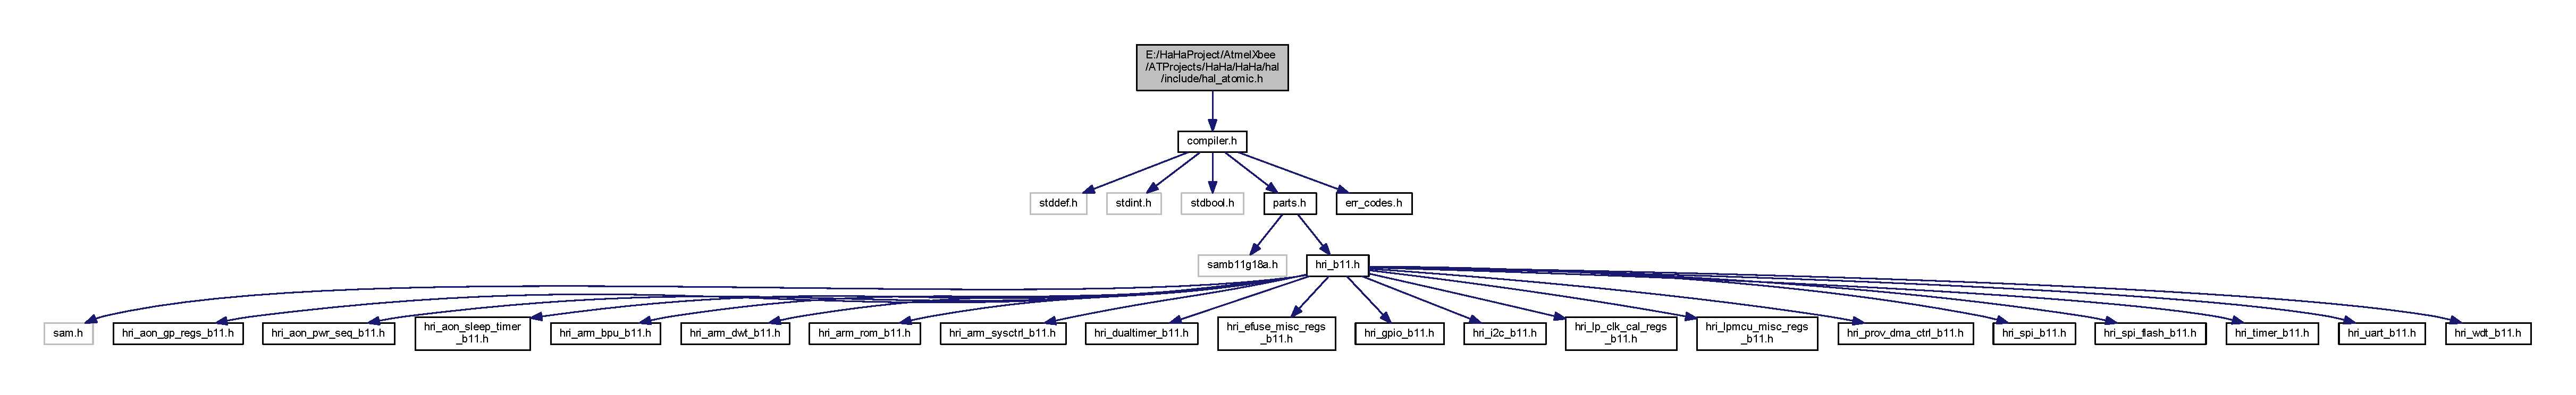
\includegraphics[width=350pt]{hal__atomic_8h__incl}
\end{center}
\end{figure}
This graph shows which files directly or indirectly include this file\+:
\nopagebreak
\begin{figure}[H]
\begin{center}
\leavevmode
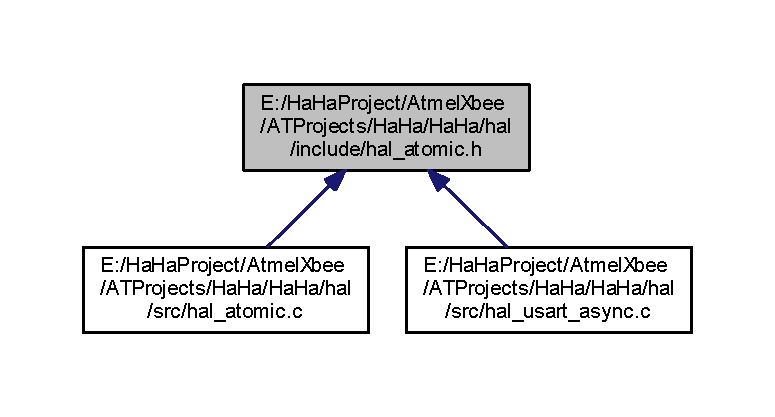
\includegraphics[width=350pt]{hal__atomic_8h__dep__incl}
\end{center}
\end{figure}
\subsection*{Macros}
\begin{DoxyCompactItemize}
\item 
\#define \hyperlink{group__doc__driver__hal__helper__atomic_ga039bfe712b6ba4388a35672f54763391}{C\+R\+I\+T\+I\+C\+A\+L\+\_\+\+S\+E\+C\+T\+I\+O\+N\+\_\+\+E\+N\+T\+ER}()
\begin{DoxyCompactList}\small\item\em Helper macro for entering critical sections. \end{DoxyCompactList}\item 
\#define \hyperlink{group__doc__driver__hal__helper__atomic_ga6b32c9f95e7c6b604d621e215c514015}{C\+R\+I\+T\+I\+C\+A\+L\+\_\+\+S\+E\+C\+T\+I\+O\+N\+\_\+\+L\+E\+A\+VE}()
\begin{DoxyCompactList}\small\item\em Helper macro for leaving critical sections. \end{DoxyCompactList}\end{DoxyCompactItemize}
\subsection*{Typedefs}
\begin{DoxyCompactItemize}
\item 
typedef uint32\+\_\+t \hyperlink{group__doc__driver__hal__helper__atomic_ga6b3a0c9eea25111ac1877e0302e2fe1c}{hal\+\_\+atomic\+\_\+t}
\begin{DoxyCompactList}\small\item\em Type for the register holding global interrupt enable flag. \end{DoxyCompactList}\end{DoxyCompactItemize}
\subsection*{Functions}
\begin{DoxyCompactItemize}
\item 
void \hyperlink{group__doc__driver__hal__helper__atomic_ga3bd20e6e0bdec53177758490510ba916}{atomic\+\_\+enter\+\_\+critical} (\hyperlink{group__doc__driver__hal__helper__atomic_ga6b3a0c9eea25111ac1877e0302e2fe1c}{hal\+\_\+atomic\+\_\+t} volatile $\ast$atomic)
\begin{DoxyCompactList}\small\item\em Disable interrupts, enter critical section. \end{DoxyCompactList}\item 
void \hyperlink{group__doc__driver__hal__helper__atomic_gaef0ccaa2438aca5ea074b36252d65990}{atomic\+\_\+leave\+\_\+critical} (\hyperlink{group__doc__driver__hal__helper__atomic_ga6b3a0c9eea25111ac1877e0302e2fe1c}{hal\+\_\+atomic\+\_\+t} volatile $\ast$atomic)
\begin{DoxyCompactList}\small\item\em Exit atomic section. \end{DoxyCompactList}\item 
uint32\+\_\+t \hyperlink{group__doc__driver__hal__helper__atomic_ga75fe13100e2799eb24a80123bc8c3787}{atomic\+\_\+get\+\_\+version} (void)
\begin{DoxyCompactList}\small\item\em Retrieve the current driver version. \end{DoxyCompactList}\end{DoxyCompactItemize}


\subsection{Detailed Description}
Critical sections related functionality declaration. 

Copyright (C) 2014 Atmel Corporation. All rights reserved.
\hypertarget{hal__gpio_8h}{}\section{E\+:/\+Ha\+Ha\+Project/\+Atmel\+Xbee/\+A\+T\+Projects/\+Ha\+Ha/\+Ha\+Ha/hal/include/hal\+\_\+gpio.h File Reference}
\label{hal__gpio_8h}\index{E\+:/\+Ha\+Ha\+Project/\+Atmel\+Xbee/\+A\+T\+Projects/\+Ha\+Ha/\+Ha\+Ha/hal/include/hal\+\_\+gpio.\+h@{E\+:/\+Ha\+Ha\+Project/\+Atmel\+Xbee/\+A\+T\+Projects/\+Ha\+Ha/\+Ha\+Ha/hal/include/hal\+\_\+gpio.\+h}}


Port.  


{\ttfamily \#include $<$hpl\+\_\+gpio.\+h$>$}\newline
{\ttfamily \#include $<$utils\+\_\+assert.\+h$>$}\newline
Include dependency graph for hal\+\_\+gpio.\+h\+:\nopagebreak
\begin{figure}[H]
\begin{center}
\leavevmode
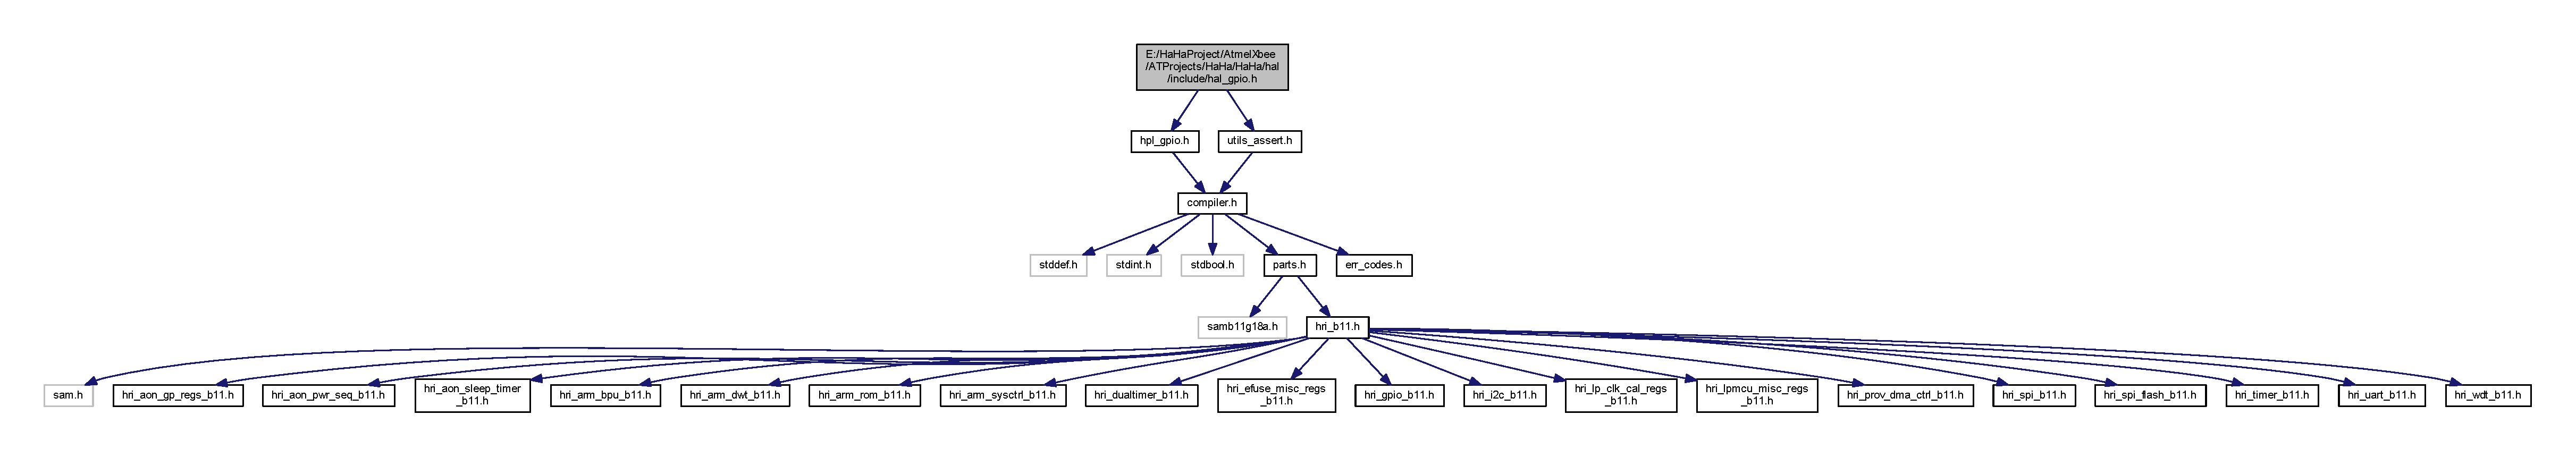
\includegraphics[width=350pt]{hal__gpio_8h__incl}
\end{center}
\end{figure}
This graph shows which files directly or indirectly include this file\+:\nopagebreak
\begin{figure}[H]
\begin{center}
\leavevmode
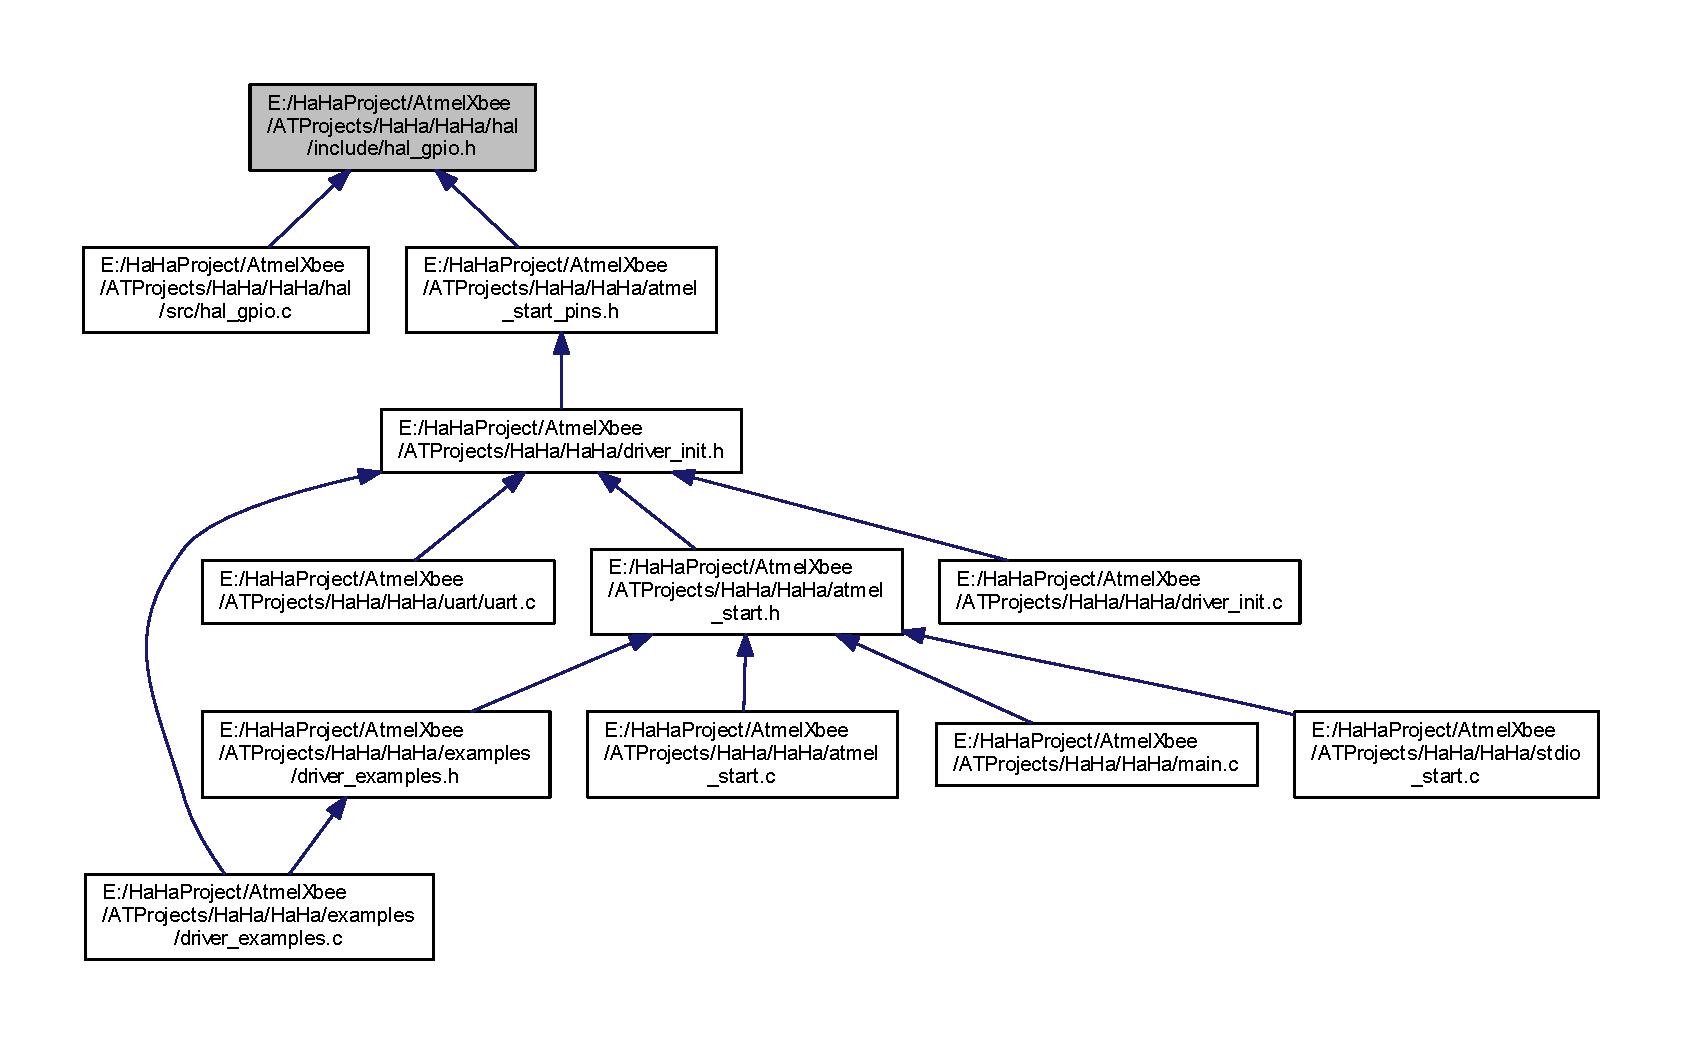
\includegraphics[width=350pt]{hal__gpio_8h__dep__incl}
\end{center}
\end{figure}
\subsection*{Functions}
\begin{DoxyCompactItemize}
\item 
uint32\+\_\+t \hyperlink{hal__gpio_8h_a19c3104daa7a427258fc4d1ba26db13b}{gpio\+\_\+get\+\_\+version} (void)
\begin{DoxyCompactList}\small\item\em Get current driver version. \end{DoxyCompactList}\end{DoxyCompactItemize}


\subsection{Detailed Description}
Port. 

Copyright (C) 2014 Atmel Corporation. All rights reserved.

\subsection{Function Documentation}
\mbox{\Hypertarget{hal__gpio_8h_a19c3104daa7a427258fc4d1ba26db13b}\label{hal__gpio_8h_a19c3104daa7a427258fc4d1ba26db13b}} 
\index{hal\+\_\+gpio.\+h@{hal\+\_\+gpio.\+h}!gpio\+\_\+get\+\_\+version@{gpio\+\_\+get\+\_\+version}}
\index{gpio\+\_\+get\+\_\+version@{gpio\+\_\+get\+\_\+version}!hal\+\_\+gpio.\+h@{hal\+\_\+gpio.\+h}}
\subsubsection{\texorpdfstring{gpio\+\_\+get\+\_\+version()}{gpio\_get\_version()}}
{\footnotesize\ttfamily uint32\+\_\+t gpio\+\_\+get\+\_\+version (\begin{DoxyParamCaption}\item[{void}]{ }\end{DoxyParamCaption})}



Get current driver version. 


\hypertarget{hal__init_8h}{}\section{E\+:/\+Ha\+Ha\+Project/\+Atmel\+Xbee/\+A\+T\+Projects/\+Ha\+Ha/\+Ha\+Ha/hal/include/hal\+\_\+init.h File Reference}
\label{hal__init_8h}\index{E\+:/\+Ha\+Ha\+Project/\+Atmel\+Xbee/\+A\+T\+Projects/\+Ha\+Ha/\+Ha\+Ha/hal/include/hal\+\_\+init.\+h@{E\+:/\+Ha\+Ha\+Project/\+Atmel\+Xbee/\+A\+T\+Projects/\+Ha\+Ha/\+Ha\+Ha/hal/include/hal\+\_\+init.\+h}}


H\+AL initialization related functionality declaration.  


{\ttfamily \#include $<$hpl\+\_\+init.\+h$>$}\newline
Include dependency graph for hal\+\_\+init.\+h\+:\nopagebreak
\begin{figure}[H]
\begin{center}
\leavevmode
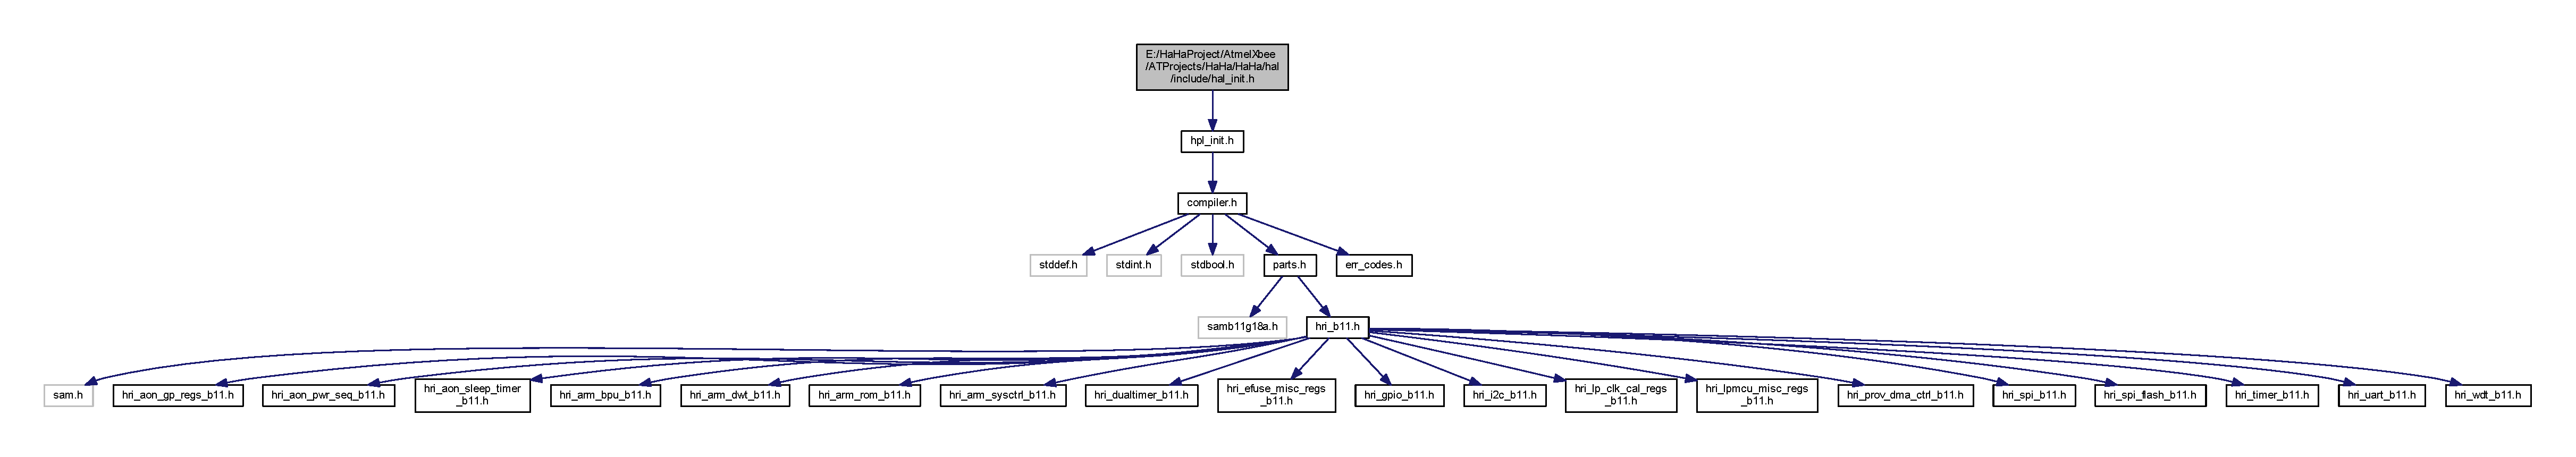
\includegraphics[width=350pt]{hal__init_8h__incl}
\end{center}
\end{figure}
This graph shows which files directly or indirectly include this file\+:\nopagebreak
\begin{figure}[H]
\begin{center}
\leavevmode
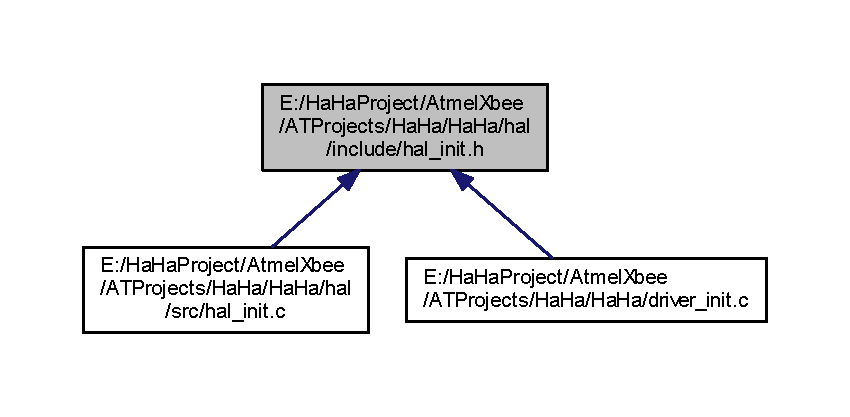
\includegraphics[width=350pt]{hal__init_8h__dep__incl}
\end{center}
\end{figure}
\subsection*{Functions}
\begin{DoxyCompactItemize}
\item 
uint32\+\_\+t \hyperlink{group__doc__driver__hal__helper__init_ga7f3a0a79c14d4043ea30435f561af05f}{init\+\_\+get\+\_\+version} (void)
\begin{DoxyCompactList}\small\item\em Retrieve the current driver version. \end{DoxyCompactList}\end{DoxyCompactItemize}


\subsection{Detailed Description}
H\+AL initialization related functionality declaration. 

Copyright (C) 2014 Atmel Corporation. All rights reserved.
\hypertarget{hal__io_8h}{}\section{E\+:/\+Ha\+Ha\+Project/\+Atmel\+Xbee/\+A\+T\+Projects/\+Ha\+Ha/\+Ha\+Ha/hal/include/hal\+\_\+io.h File Reference}
\label{hal__io_8h}\index{E\+:/\+Ha\+Ha\+Project/\+Atmel\+Xbee/\+A\+T\+Projects/\+Ha\+Ha/\+Ha\+Ha/hal/include/hal\+\_\+io.\+h@{E\+:/\+Ha\+Ha\+Project/\+Atmel\+Xbee/\+A\+T\+Projects/\+Ha\+Ha/\+Ha\+Ha/hal/include/hal\+\_\+io.\+h}}


IO related functionality declaration.  


{\ttfamily \#include $<$compiler.\+h$>$}\newline
Include dependency graph for hal\+\_\+io.\+h\+:
\nopagebreak
\begin{figure}[H]
\begin{center}
\leavevmode
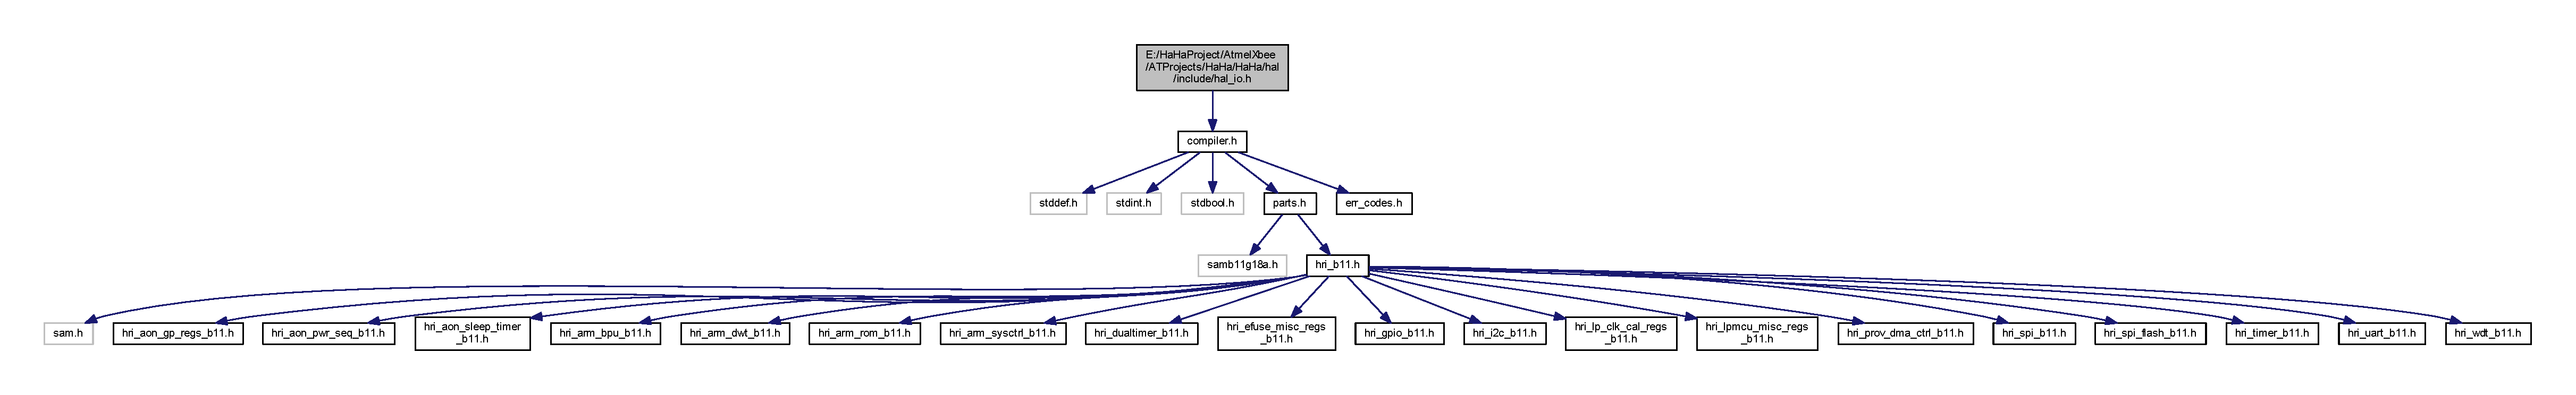
\includegraphics[width=350pt]{hal__io_8h__incl}
\end{center}
\end{figure}
This graph shows which files directly or indirectly include this file\+:
\nopagebreak
\begin{figure}[H]
\begin{center}
\leavevmode
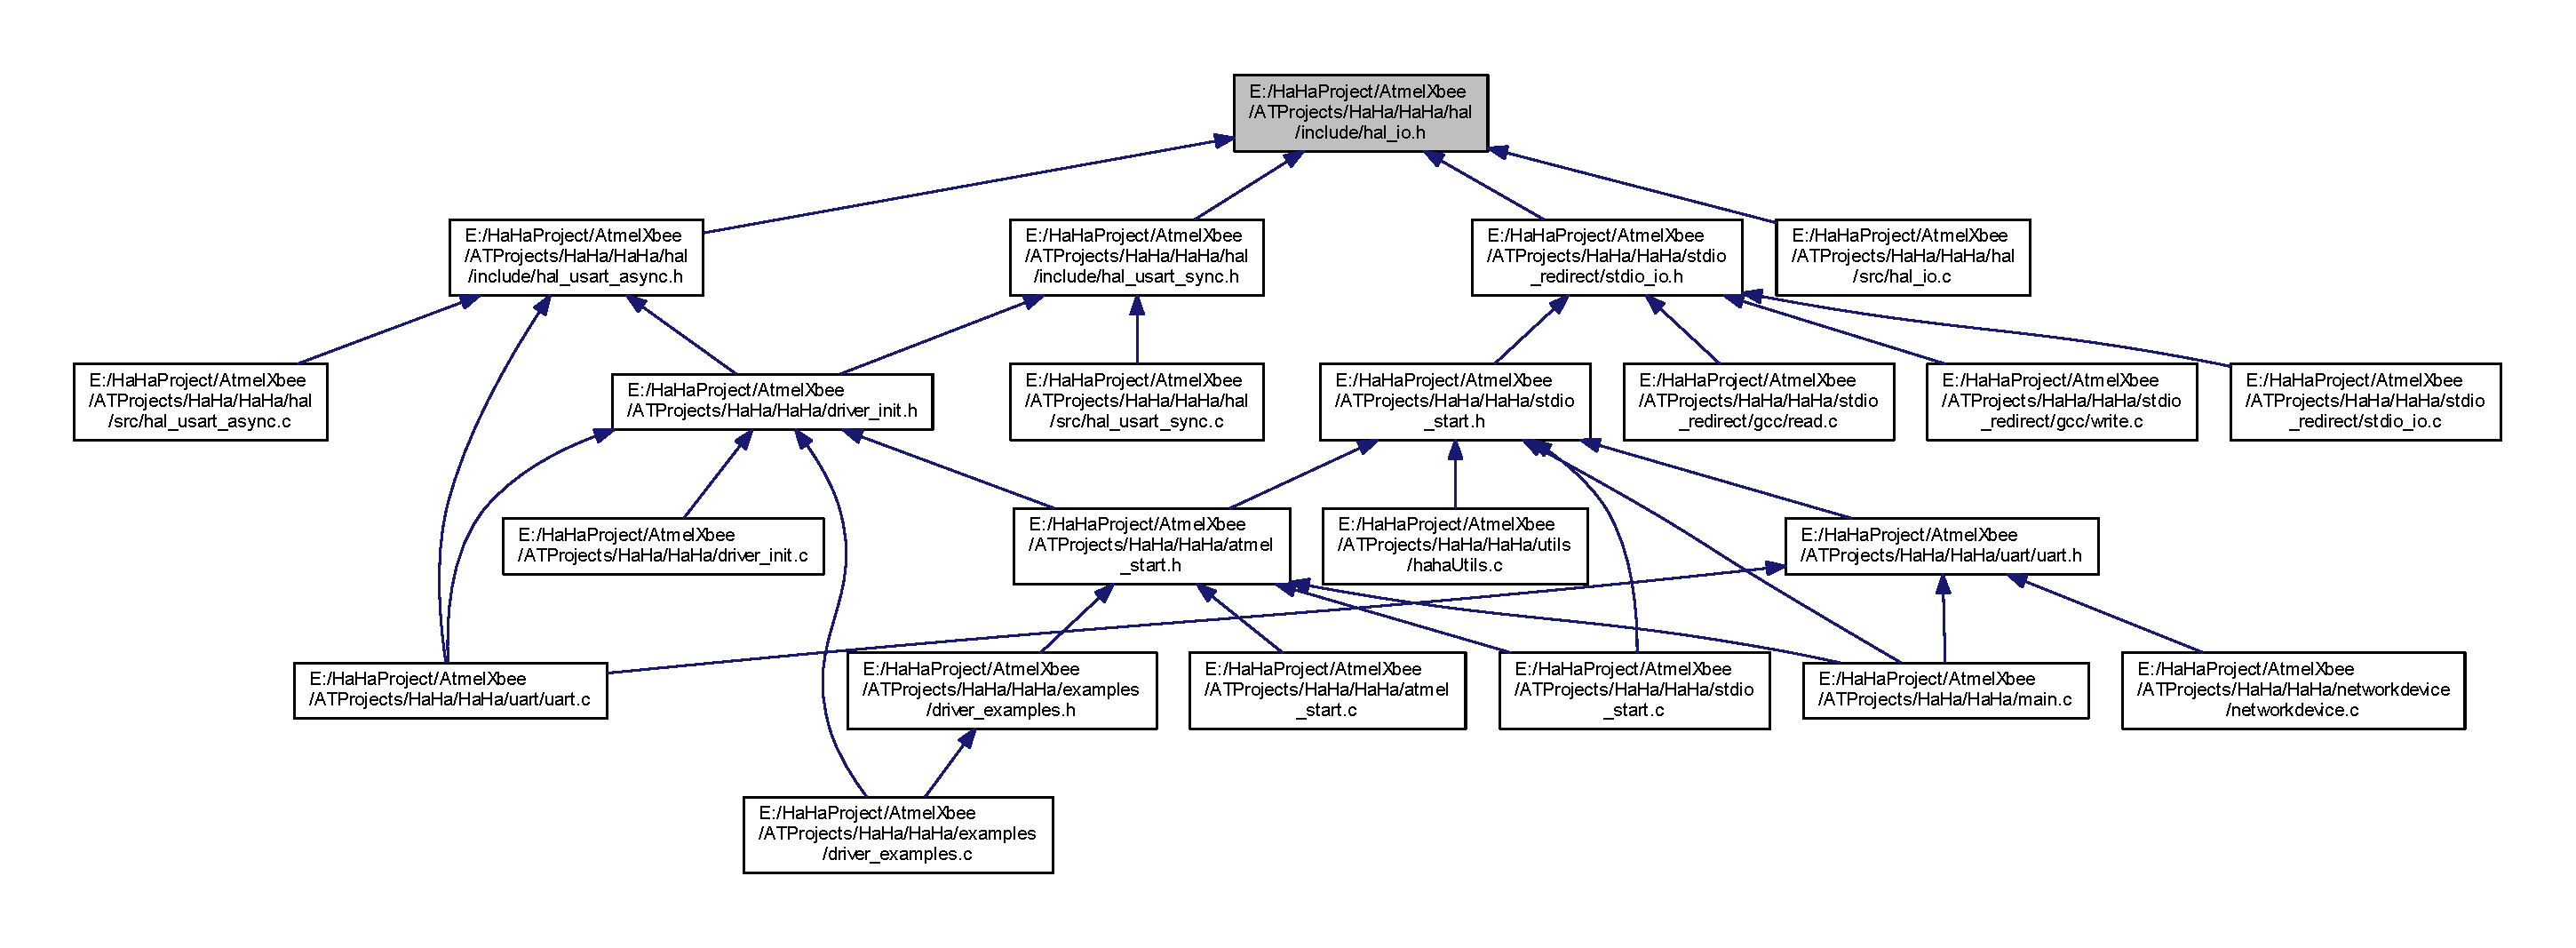
\includegraphics[width=350pt]{hal__io_8h__dep__incl}
\end{center}
\end{figure}
\subsection*{Classes}
\begin{DoxyCompactItemize}
\item 
struct \hyperlink{structio__descriptor}{io\+\_\+descriptor}
\begin{DoxyCompactList}\small\item\em IO descriptor. \end{DoxyCompactList}\end{DoxyCompactItemize}
\subsection*{Typedefs}
\begin{DoxyCompactItemize}
\item 
typedef int32\+\_\+t($\ast$ \hyperlink{group__doc__driver__hal__helper__io_gacb03c48993a6786f00946c196c40add1}{io\+\_\+write\+\_\+t}) (struct \hyperlink{structio__descriptor}{io\+\_\+descriptor} $\ast$const io\+\_\+descr, const uint8\+\_\+t $\ast$const buf, const uint16\+\_\+t length)
\begin{DoxyCompactList}\small\item\em IO write function pointer type. \end{DoxyCompactList}\item 
typedef int32\+\_\+t($\ast$ \hyperlink{group__doc__driver__hal__helper__io_ga4d9ae58de2887289fe09eac6f0aa8be7}{io\+\_\+read\+\_\+t}) (struct \hyperlink{structio__descriptor}{io\+\_\+descriptor} $\ast$const io\+\_\+descr, uint8\+\_\+t $\ast$const buf, const uint16\+\_\+t length)
\begin{DoxyCompactList}\small\item\em IO read function pointer type. \end{DoxyCompactList}\end{DoxyCompactItemize}
\subsection*{Functions}
\begin{DoxyCompactItemize}
\item 
int32\+\_\+t \hyperlink{group__doc__driver__hal__helper__io_ga81aac60d5ce6feb0c44f8937d7c02f14}{io\+\_\+write} (struct \hyperlink{structio__descriptor}{io\+\_\+descriptor} $\ast$const io\+\_\+descr, const uint8\+\_\+t $\ast$const buf, const uint16\+\_\+t length)
\begin{DoxyCompactList}\small\item\em IO write interface. \end{DoxyCompactList}\item 
int32\+\_\+t \hyperlink{group__doc__driver__hal__helper__io_gaf5e8722129933fa8e014144fd7505be6}{io\+\_\+read} (struct \hyperlink{structio__descriptor}{io\+\_\+descriptor} $\ast$const io\+\_\+descr, uint8\+\_\+t $\ast$const buf, const uint16\+\_\+t length)
\begin{DoxyCompactList}\small\item\em IO read interface. \end{DoxyCompactList}\end{DoxyCompactItemize}


\subsection{Detailed Description}
IO related functionality declaration. 

Copyright (C) 2014 -\/ 2016 Atmel Corporation. All rights reserved.
\hypertarget{hal__usart__async_8h}{}\section{E\+:/\+Ha\+Ha\+Project/\+Atmel\+Xbee/\+A\+T\+Projects/\+Ha\+Ha/\+Ha\+Ha/hal/include/hal\+\_\+usart\+\_\+async.h File Reference}
\label{hal__usart__async_8h}\index{E\+:/\+Ha\+Ha\+Project/\+Atmel\+Xbee/\+A\+T\+Projects/\+Ha\+Ha/\+Ha\+Ha/hal/include/hal\+\_\+usart\+\_\+async.\+h@{E\+:/\+Ha\+Ha\+Project/\+Atmel\+Xbee/\+A\+T\+Projects/\+Ha\+Ha/\+Ha\+Ha/hal/include/hal\+\_\+usart\+\_\+async.\+h}}


U\+S\+A\+RT related functionality declaration.  


{\ttfamily \#include \char`\"{}hal\+\_\+io.\+h\char`\"{}}\newline
{\ttfamily \#include $<$hpl\+\_\+usart\+\_\+async.\+h$>$}\newline
{\ttfamily \#include $<$utils\+\_\+ringbuffer.\+h$>$}\newline
Include dependency graph for hal\+\_\+usart\+\_\+async.\+h\+:
\nopagebreak
\begin{figure}[H]
\begin{center}
\leavevmode
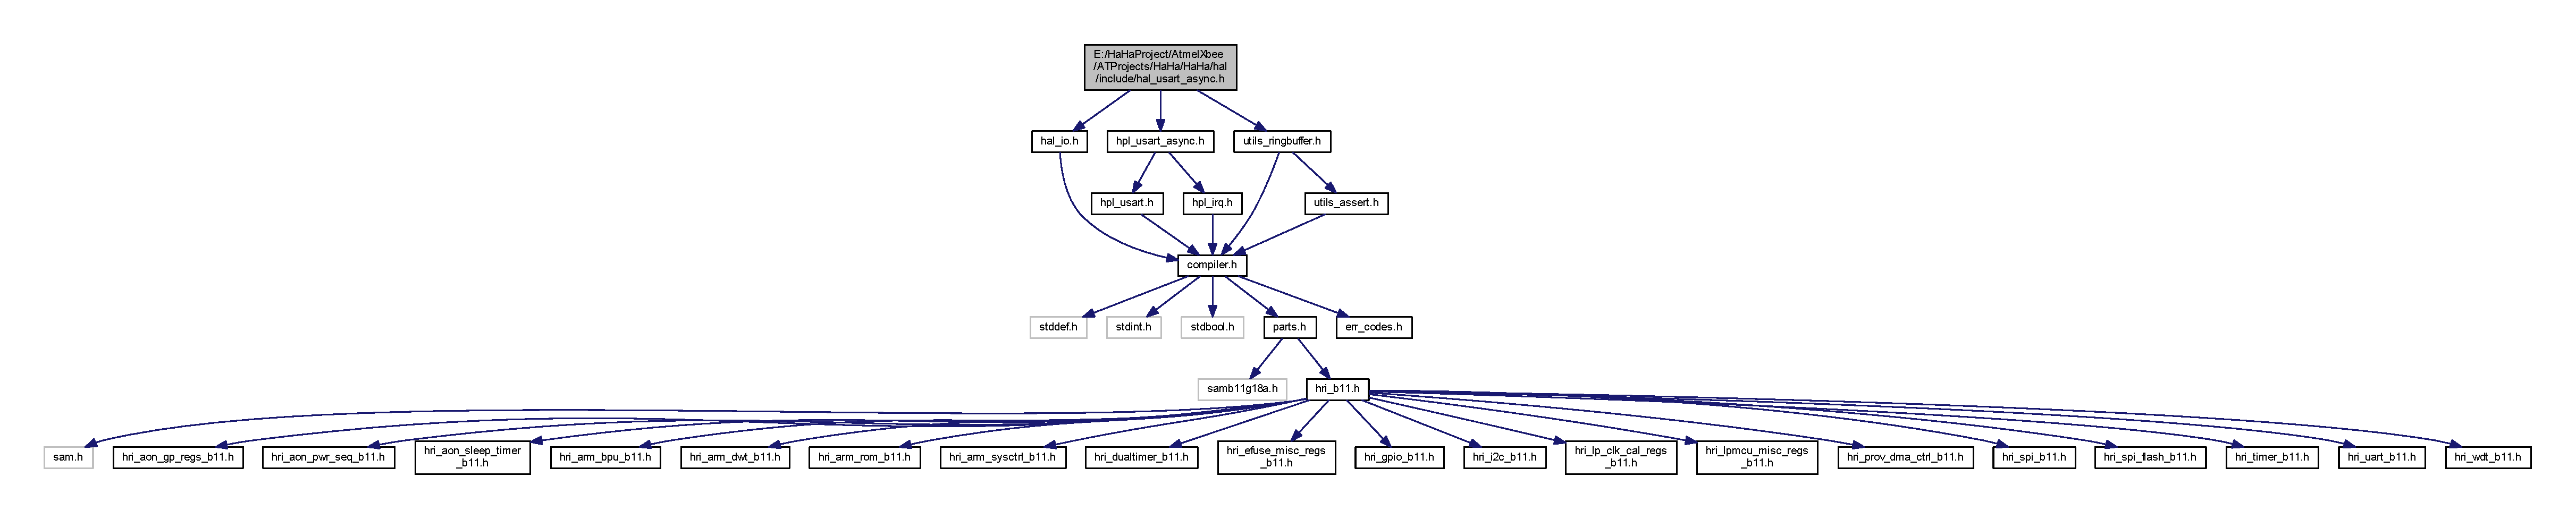
\includegraphics[width=350pt]{hal__usart__async_8h__incl}
\end{center}
\end{figure}
This graph shows which files directly or indirectly include this file\+:
\nopagebreak
\begin{figure}[H]
\begin{center}
\leavevmode
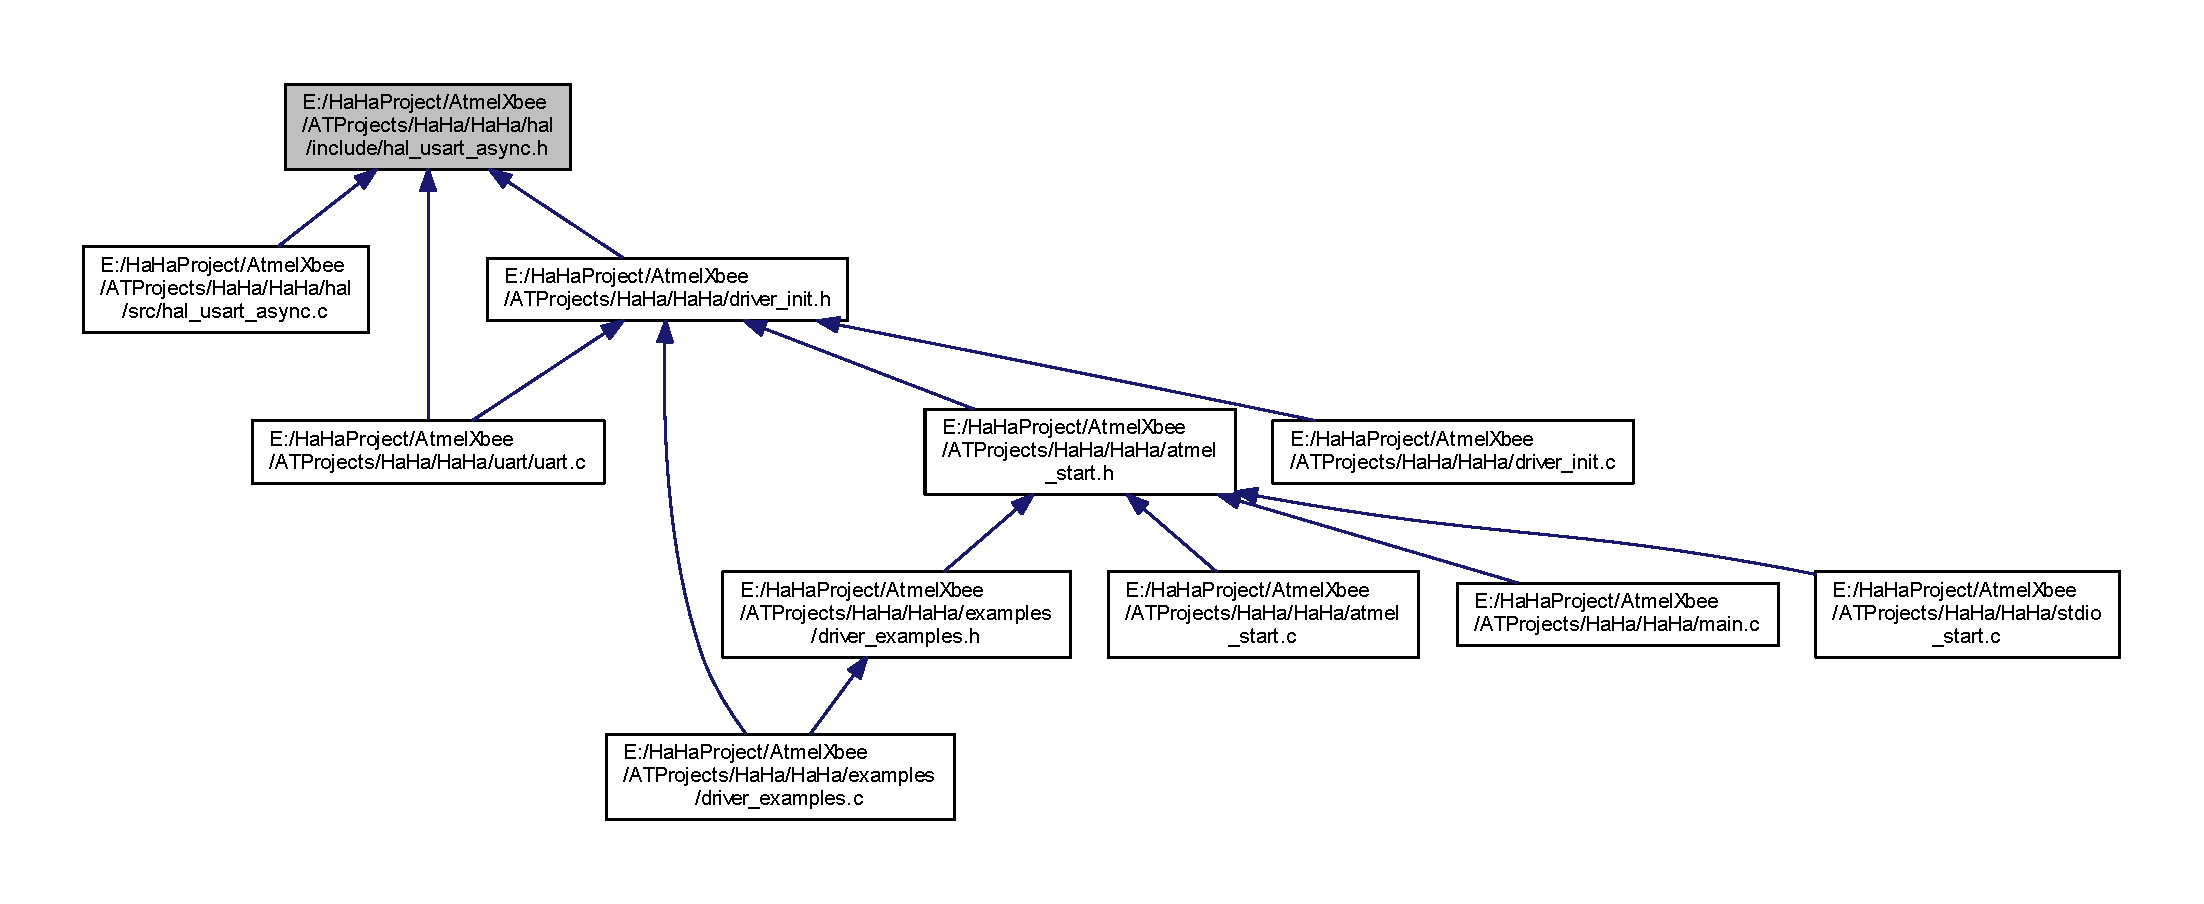
\includegraphics[width=350pt]{hal__usart__async_8h__dep__incl}
\end{center}
\end{figure}
\subsection*{Classes}
\begin{DoxyCompactItemize}
\item 
struct \hyperlink{structusart__async__callbacks}{usart\+\_\+async\+\_\+callbacks}
\begin{DoxyCompactList}\small\item\em U\+S\+A\+RT callbacks. \end{DoxyCompactList}\item 
struct \hyperlink{structusart__async__status}{usart\+\_\+async\+\_\+status}
\begin{DoxyCompactList}\small\item\em U\+S\+A\+RT status Status descriptor holds the current status of transfer. \end{DoxyCompactList}\item 
struct \hyperlink{structusart__async__descriptor}{usart\+\_\+async\+\_\+descriptor}
\begin{DoxyCompactList}\small\item\em Asynchronous U\+S\+A\+RT descriptor structure. \end{DoxyCompactList}\end{DoxyCompactItemize}
\subsection*{Macros}
\begin{DoxyCompactItemize}
\item 
\#define \hyperlink{group__doc__driver__hal__usart__async_ga6991341cd882eb58bccc1de667d1b336}{U\+S\+A\+R\+T\+\_\+\+A\+S\+Y\+N\+C\+\_\+\+S\+T\+A\+T\+U\+S\+\_\+\+B\+U\+SY}~0x0001
\end{DoxyCompactItemize}
\subsection*{Typedefs}
\begin{DoxyCompactItemize}
\item 
typedef void($\ast$ \hyperlink{group__doc__driver__hal__usart__async_ga430e4080a53e1f39c4d46da01200f633}{usart\+\_\+cb\+\_\+t}) (const struct \hyperlink{structusart__async__descriptor}{usart\+\_\+async\+\_\+descriptor} $\ast$const descr)
\begin{DoxyCompactList}\small\item\em U\+S\+A\+RT callback type. \end{DoxyCompactList}\end{DoxyCompactItemize}
\subsection*{Enumerations}
\begin{DoxyCompactItemize}
\item 
enum \hyperlink{group__doc__driver__hal__usart__async_ga5a82ef383f62daa061a55838c8fc6d39}{usart\+\_\+async\+\_\+callback\+\_\+type} \{ \hyperlink{group__doc__driver__hal__usart__async_gga5a82ef383f62daa061a55838c8fc6d39a53f74860827af0c754db79111ea4a8af}{U\+S\+A\+R\+T\+\_\+\+A\+S\+Y\+N\+C\+\_\+\+R\+X\+C\+\_\+\+CB}, 
\hyperlink{group__doc__driver__hal__usart__async_gga5a82ef383f62daa061a55838c8fc6d39a72dc4487f710fa4b902fbd97a0dbe391}{U\+S\+A\+R\+T\+\_\+\+A\+S\+Y\+N\+C\+\_\+\+T\+X\+C\+\_\+\+CB}, 
\hyperlink{group__doc__driver__hal__usart__async_gga5a82ef383f62daa061a55838c8fc6d39a5dff48ffecc0bfaf55c0fbc9f27ca8d2}{U\+S\+A\+R\+T\+\_\+\+A\+S\+Y\+N\+C\+\_\+\+E\+R\+R\+O\+R\+\_\+\+CB}
 \}\begin{DoxyCompactList}\small\item\em U\+S\+A\+RT callback types. \end{DoxyCompactList}
\end{DoxyCompactItemize}
\subsection*{Functions}
\begin{DoxyCompactItemize}
\item 
int32\+\_\+t \hyperlink{group__doc__driver__hal__usart__async_gaafe146c618b950c9715efb0fdc6a7484}{usart\+\_\+async\+\_\+init} (struct \hyperlink{structusart__async__descriptor}{usart\+\_\+async\+\_\+descriptor} $\ast$const descr, void $\ast$const hw, uint8\+\_\+t $\ast$const rx\+\_\+buffer, const uint16\+\_\+t rx\+\_\+buffer\+\_\+length, void $\ast$const func)
\begin{DoxyCompactList}\small\item\em Initialize usart interface. \end{DoxyCompactList}\item 
int32\+\_\+t \hyperlink{group__doc__driver__hal__usart__async_gab7ef65ba7b4afd13cb11dcc72315ca43}{usart\+\_\+async\+\_\+deinit} (struct \hyperlink{structusart__async__descriptor}{usart\+\_\+async\+\_\+descriptor} $\ast$const descr)
\begin{DoxyCompactList}\small\item\em De-\/initialize usart interface. \end{DoxyCompactList}\item 
int32\+\_\+t \hyperlink{group__doc__driver__hal__usart__async_gaa752e7d978b7f3bc35c97f9a7eb5f98a}{usart\+\_\+async\+\_\+enable} (struct \hyperlink{structusart__async__descriptor}{usart\+\_\+async\+\_\+descriptor} $\ast$const descr)
\begin{DoxyCompactList}\small\item\em Enable usart interface. \end{DoxyCompactList}\item 
int32\+\_\+t \hyperlink{group__doc__driver__hal__usart__async_ga575b7b546a7357088530a9cebf60ad9a}{usart\+\_\+async\+\_\+disable} (struct \hyperlink{structusart__async__descriptor}{usart\+\_\+async\+\_\+descriptor} $\ast$const descr)
\begin{DoxyCompactList}\small\item\em Disable usart interface. \end{DoxyCompactList}\item 
int32\+\_\+t \hyperlink{group__doc__driver__hal__usart__async_ga964be25acbad24e7d0cb9e72f5f5582f}{usart\+\_\+async\+\_\+get\+\_\+io\+\_\+descriptor} (struct \hyperlink{structusart__async__descriptor}{usart\+\_\+async\+\_\+descriptor} $\ast$const descr, struct \hyperlink{structio__descriptor}{io\+\_\+descriptor} $\ast$$\ast$io)
\begin{DoxyCompactList}\small\item\em Retrieve IO descriptor. \end{DoxyCompactList}\item 
int32\+\_\+t \hyperlink{group__doc__driver__hal__usart__async_ga2d7d4ba3ab10f19c2e8a7901f2b6b276}{usart\+\_\+async\+\_\+register\+\_\+callback} (struct \hyperlink{structusart__async__descriptor}{usart\+\_\+async\+\_\+descriptor} $\ast$const descr, const enum \hyperlink{group__doc__driver__hal__usart__async_ga5a82ef383f62daa061a55838c8fc6d39}{usart\+\_\+async\+\_\+callback\+\_\+type} type, \hyperlink{group__doc__driver__hal__usart__async_ga430e4080a53e1f39c4d46da01200f633}{usart\+\_\+cb\+\_\+t} cb)
\begin{DoxyCompactList}\small\item\em Register usart callback. \end{DoxyCompactList}\item 
int32\+\_\+t \hyperlink{group__doc__driver__hal__usart__async_gacbc3f9aec99169e42d49555cf829a3d1}{usart\+\_\+async\+\_\+set\+\_\+flow\+\_\+control} (struct \hyperlink{structusart__async__descriptor}{usart\+\_\+async\+\_\+descriptor} $\ast$const descr, const union \hyperlink{unionusart__flow__control__state}{usart\+\_\+flow\+\_\+control\+\_\+state} state)
\begin{DoxyCompactList}\small\item\em Specify action for flow control pins. \end{DoxyCompactList}\item 
int32\+\_\+t \hyperlink{group__doc__driver__hal__usart__async_gab6bb473a5047ae890b1406ffcca3042d}{usart\+\_\+async\+\_\+set\+\_\+baud\+\_\+rate} (struct \hyperlink{structusart__async__descriptor}{usart\+\_\+async\+\_\+descriptor} $\ast$const descr, const uint32\+\_\+t baud\+\_\+rate)
\begin{DoxyCompactList}\small\item\em Set usart baud rate. \end{DoxyCompactList}\item 
int32\+\_\+t \hyperlink{group__doc__driver__hal__usart__async_ga1ed416c72b54e87f8da098f148e0c7fc}{usart\+\_\+async\+\_\+set\+\_\+data\+\_\+order} (struct \hyperlink{structusart__async__descriptor}{usart\+\_\+async\+\_\+descriptor} $\ast$const descr, const enum \hyperlink{group___h_p_l_ga426849bbd9655cec091101ebc9123eb4}{usart\+\_\+data\+\_\+order} data\+\_\+order)
\begin{DoxyCompactList}\small\item\em Set usart data order. \end{DoxyCompactList}\item 
int32\+\_\+t \hyperlink{group__doc__driver__hal__usart__async_ga8b2ee777456a88b7843366761a8356c9}{usart\+\_\+async\+\_\+set\+\_\+mode} (struct \hyperlink{structusart__async__descriptor}{usart\+\_\+async\+\_\+descriptor} $\ast$const descr, const enum \hyperlink{group___h_p_l_ga1c465965478e0f6908a4c99d4f3ad20f}{usart\+\_\+mode} mode)
\begin{DoxyCompactList}\small\item\em Set usart mode. \end{DoxyCompactList}\item 
int32\+\_\+t \hyperlink{group__doc__driver__hal__usart__async_ga6cee441159bf41f74a105042fb6c8477}{usart\+\_\+async\+\_\+set\+\_\+parity} (struct \hyperlink{structusart__async__descriptor}{usart\+\_\+async\+\_\+descriptor} $\ast$const descr, const enum \hyperlink{group___h_p_l_ga867cc5f0ea7d3bf651d68f0046cf6f41}{usart\+\_\+parity} parity)
\begin{DoxyCompactList}\small\item\em Set usart parity. \end{DoxyCompactList}\item 
int32\+\_\+t \hyperlink{group__doc__driver__hal__usart__async_ga1749b4fd6293a49428cf4baf74656dd5}{usart\+\_\+async\+\_\+set\+\_\+stopbits} (struct \hyperlink{structusart__async__descriptor}{usart\+\_\+async\+\_\+descriptor} $\ast$const descr, const enum \hyperlink{group___h_p_l_ga88311517c5168c29a681604a8a33b06e}{usart\+\_\+stop\+\_\+bits} stop\+\_\+bits)
\begin{DoxyCompactList}\small\item\em Set usart stop bits. \end{DoxyCompactList}\item 
int32\+\_\+t \hyperlink{group__doc__driver__hal__usart__async_ga949ebae93032ed1a276be009cc1539d6}{usart\+\_\+async\+\_\+set\+\_\+character\+\_\+size} (struct \hyperlink{structusart__async__descriptor}{usart\+\_\+async\+\_\+descriptor} $\ast$const descr, const enum \hyperlink{group___h_p_l_ga631ce7b4f60dccd392e6d6ef7d3cd4e2}{usart\+\_\+character\+\_\+size} size)
\begin{DoxyCompactList}\small\item\em Set usart character size. \end{DoxyCompactList}\item 
int32\+\_\+t \hyperlink{group__doc__driver__hal__usart__async_gaf451cb5a13be66b9357354b1b503c892}{usart\+\_\+async\+\_\+flow\+\_\+control\+\_\+status} (const struct \hyperlink{structusart__async__descriptor}{usart\+\_\+async\+\_\+descriptor} $\ast$const descr, union \hyperlink{unionusart__flow__control__state}{usart\+\_\+flow\+\_\+control\+\_\+state} $\ast$const state)
\begin{DoxyCompactList}\small\item\em Retrieve the state of flow control pins. \end{DoxyCompactList}\item 
int32\+\_\+t \hyperlink{group__doc__driver__hal__usart__async_ga25db066e0587014aab7038cc9295b177}{usart\+\_\+async\+\_\+is\+\_\+tx\+\_\+empty} (const struct \hyperlink{structusart__async__descriptor}{usart\+\_\+async\+\_\+descriptor} $\ast$const descr)
\begin{DoxyCompactList}\small\item\em Check if the usart transmitter is empty. \end{DoxyCompactList}\item 
int32\+\_\+t \hyperlink{group__doc__driver__hal__usart__async_gac8f1c592dc9a82c918eb5c7b2d036963}{usart\+\_\+async\+\_\+is\+\_\+rx\+\_\+not\+\_\+empty} (const struct \hyperlink{structusart__async__descriptor}{usart\+\_\+async\+\_\+descriptor} $\ast$const descr)
\begin{DoxyCompactList}\small\item\em Check if the usart receiver is not empty. \end{DoxyCompactList}\item 
int32\+\_\+t \hyperlink{group__doc__driver__hal__usart__async_gabf0f8fdd20b3b586cb5c0d7fcd4e2114}{usart\+\_\+async\+\_\+get\+\_\+status} (struct \hyperlink{structusart__async__descriptor}{usart\+\_\+async\+\_\+descriptor} $\ast$const descr, struct \hyperlink{structusart__async__status}{usart\+\_\+async\+\_\+status} $\ast$const status)
\begin{DoxyCompactList}\small\item\em Retrieve the current interface status. \end{DoxyCompactList}\item 
int32\+\_\+t \hyperlink{group__doc__driver__hal__usart__async_gaaccb76b1f2ca76451e29b1f674a0c646}{usart\+\_\+async\+\_\+flush\+\_\+rx\+\_\+buffer} (struct \hyperlink{structusart__async__descriptor}{usart\+\_\+async\+\_\+descriptor} $\ast$const descr)
\begin{DoxyCompactList}\small\item\em flush usart ringbuf \end{DoxyCompactList}\item 
uint32\+\_\+t \hyperlink{group__doc__driver__hal__usart__async_ga8fd83888546106a6a65e1951e4065d9f}{usart\+\_\+async\+\_\+get\+\_\+version} (void)
\begin{DoxyCompactList}\small\item\em Retrieve the current driver version. \end{DoxyCompactList}\end{DoxyCompactItemize}


\subsection{Detailed Description}
U\+S\+A\+RT related functionality declaration. 

Copyright (C) 2014 Atmel Corporation. All rights reserved.
\hypertarget{hal__usart__sync_8h}{}\section{E\+:/\+Ha\+Ha\+Project/\+Atmel\+Xbee/\+A\+T\+Projects/\+Ha\+Ha/\+Ha\+Ha/hal/include/hal\+\_\+usart\+\_\+sync.h File Reference}
\label{hal__usart__sync_8h}\index{E\+:/\+Ha\+Ha\+Project/\+Atmel\+Xbee/\+A\+T\+Projects/\+Ha\+Ha/\+Ha\+Ha/hal/include/hal\+\_\+usart\+\_\+sync.\+h@{E\+:/\+Ha\+Ha\+Project/\+Atmel\+Xbee/\+A\+T\+Projects/\+Ha\+Ha/\+Ha\+Ha/hal/include/hal\+\_\+usart\+\_\+sync.\+h}}


U\+S\+A\+RT related functionality declaration.  


{\ttfamily \#include \char`\"{}hal\+\_\+io.\+h\char`\"{}}\newline
{\ttfamily \#include $<$hpl\+\_\+usart\+\_\+sync.\+h$>$}\newline
\subsection*{Classes}
\begin{DoxyCompactItemize}
\item 
struct \hyperlink{structusart__sync__descriptor}{usart\+\_\+sync\+\_\+descriptor}
\begin{DoxyCompactList}\small\item\em Synchronous U\+S\+A\+RT descriptor. \end{DoxyCompactList}\end{DoxyCompactItemize}
\subsection*{Functions}
\begin{DoxyCompactItemize}
\item 
int32\+\_\+t \hyperlink{group__doc__driver__hal__usart__sync_gaa3cca792d7af7f180c5084af8ffd11c3}{usart\+\_\+sync\+\_\+init} (struct \hyperlink{structusart__sync__descriptor}{usart\+\_\+sync\+\_\+descriptor} $\ast$const descr, void $\ast$const hw, void $\ast$const func)
\begin{DoxyCompactList}\small\item\em Initialize usart interface. \end{DoxyCompactList}\item 
int32\+\_\+t \hyperlink{group__doc__driver__hal__usart__sync_gae8076ed0a30199bd526f1da22e2095d3}{usart\+\_\+sync\+\_\+deinit} (struct \hyperlink{structusart__sync__descriptor}{usart\+\_\+sync\+\_\+descriptor} $\ast$const descr)
\begin{DoxyCompactList}\small\item\em De-\/initialize usart interface. \end{DoxyCompactList}\item 
int32\+\_\+t \hyperlink{group__doc__driver__hal__usart__sync_ga351aa9c8c94b4e8b0eb5efb1ecd74a82}{usart\+\_\+sync\+\_\+enable} (struct \hyperlink{structusart__sync__descriptor}{usart\+\_\+sync\+\_\+descriptor} $\ast$const descr)
\begin{DoxyCompactList}\small\item\em Enable usart interface. \end{DoxyCompactList}\item 
int32\+\_\+t \hyperlink{group__doc__driver__hal__usart__sync_ga76abe691b76e4b95b4e3a7d5bc79b026}{usart\+\_\+sync\+\_\+disable} (struct \hyperlink{structusart__sync__descriptor}{usart\+\_\+sync\+\_\+descriptor} $\ast$const descr)
\begin{DoxyCompactList}\small\item\em Disable usart interface. \end{DoxyCompactList}\item 
int32\+\_\+t \hyperlink{group__doc__driver__hal__usart__sync_gaf0b9c8819dc24f75e4f87f050edc81f5}{usart\+\_\+sync\+\_\+get\+\_\+io\+\_\+descriptor} (struct \hyperlink{structusart__sync__descriptor}{usart\+\_\+sync\+\_\+descriptor} $\ast$const descr, struct \hyperlink{structio__descriptor}{io\+\_\+descriptor} $\ast$$\ast$io)
\begin{DoxyCompactList}\small\item\em Retrieve IO descriptor. \end{DoxyCompactList}\item 
int32\+\_\+t \hyperlink{group__doc__driver__hal__usart__sync_ga23977cbdcabc4a624dde31be5ebba482}{usart\+\_\+sync\+\_\+set\+\_\+flow\+\_\+control} (struct \hyperlink{structusart__sync__descriptor}{usart\+\_\+sync\+\_\+descriptor} $\ast$const descr, const union \hyperlink{unionusart__flow__control__state}{usart\+\_\+flow\+\_\+control\+\_\+state} state)
\begin{DoxyCompactList}\small\item\em Specify action for flow control pins. \end{DoxyCompactList}\item 
int32\+\_\+t \hyperlink{group__doc__driver__hal__usart__sync_gaa6c286d38362477d8d11e0d2a46b6b19}{usart\+\_\+sync\+\_\+set\+\_\+baud\+\_\+rate} (struct \hyperlink{structusart__sync__descriptor}{usart\+\_\+sync\+\_\+descriptor} $\ast$const descr, const uint32\+\_\+t baud\+\_\+rate)
\begin{DoxyCompactList}\small\item\em Set usart baud rate. \end{DoxyCompactList}\item 
int32\+\_\+t \hyperlink{group__doc__driver__hal__usart__sync_ga4f750fb4f18d022fe95ca98a434a9f28}{usart\+\_\+sync\+\_\+set\+\_\+data\+\_\+order} (struct \hyperlink{structusart__sync__descriptor}{usart\+\_\+sync\+\_\+descriptor} $\ast$const descr, const enum \hyperlink{group___h_p_l_ga426849bbd9655cec091101ebc9123eb4}{usart\+\_\+data\+\_\+order} data\+\_\+order)
\begin{DoxyCompactList}\small\item\em Set usart data order. \end{DoxyCompactList}\item 
int32\+\_\+t \hyperlink{group__doc__driver__hal__usart__sync_gad9c806a6bb34a0cd643e922db4561a7e}{usart\+\_\+sync\+\_\+set\+\_\+mode} (struct \hyperlink{structusart__sync__descriptor}{usart\+\_\+sync\+\_\+descriptor} $\ast$const descr, const enum \hyperlink{group___h_p_l_ga1c465965478e0f6908a4c99d4f3ad20f}{usart\+\_\+mode} mode)
\begin{DoxyCompactList}\small\item\em Set usart mode. \end{DoxyCompactList}\item 
int32\+\_\+t \hyperlink{group__doc__driver__hal__usart__sync_ga69fa5d85a169234c2da5b9c82dc1996a}{usart\+\_\+sync\+\_\+set\+\_\+parity} (struct \hyperlink{structusart__sync__descriptor}{usart\+\_\+sync\+\_\+descriptor} $\ast$const descr, const enum \hyperlink{group___h_p_l_ga867cc5f0ea7d3bf651d68f0046cf6f41}{usart\+\_\+parity} parity)
\begin{DoxyCompactList}\small\item\em Set usart parity. \end{DoxyCompactList}\item 
int32\+\_\+t \hyperlink{group__doc__driver__hal__usart__sync_ga51ced5cb2b2a5ac61f17a41e87739dde}{usart\+\_\+sync\+\_\+set\+\_\+stopbits} (struct \hyperlink{structusart__sync__descriptor}{usart\+\_\+sync\+\_\+descriptor} $\ast$const descr, const enum \hyperlink{group___h_p_l_ga88311517c5168c29a681604a8a33b06e}{usart\+\_\+stop\+\_\+bits} stop\+\_\+bits)
\begin{DoxyCompactList}\small\item\em Set usart stop bits. \end{DoxyCompactList}\item 
int32\+\_\+t \hyperlink{group__doc__driver__hal__usart__sync_ga11ad11c2436f8315ff90f9868aaa5b84}{usart\+\_\+sync\+\_\+set\+\_\+character\+\_\+size} (struct \hyperlink{structusart__sync__descriptor}{usart\+\_\+sync\+\_\+descriptor} $\ast$const descr, const enum \hyperlink{group___h_p_l_ga631ce7b4f60dccd392e6d6ef7d3cd4e2}{usart\+\_\+character\+\_\+size} size)
\begin{DoxyCompactList}\small\item\em Set usart character size. \end{DoxyCompactList}\item 
int32\+\_\+t \hyperlink{group__doc__driver__hal__usart__sync_ga34932fa96b2190715b37f2c2c784a2f4}{usart\+\_\+sync\+\_\+flow\+\_\+control\+\_\+status} (const struct \hyperlink{structusart__sync__descriptor}{usart\+\_\+sync\+\_\+descriptor} $\ast$const descr, union \hyperlink{unionusart__flow__control__state}{usart\+\_\+flow\+\_\+control\+\_\+state} $\ast$const state)
\begin{DoxyCompactList}\small\item\em Retrieve the state of flow control pins. \end{DoxyCompactList}\item 
int32\+\_\+t \hyperlink{group__doc__driver__hal__usart__sync_ga9620a8556a276388486b87b5a2e3ce6d}{usart\+\_\+sync\+\_\+is\+\_\+tx\+\_\+empty} (const struct \hyperlink{structusart__sync__descriptor}{usart\+\_\+sync\+\_\+descriptor} $\ast$const descr)
\begin{DoxyCompactList}\small\item\em Check if the usart transmitter is empty. \end{DoxyCompactList}\item 
int32\+\_\+t \hyperlink{group__doc__driver__hal__usart__sync_ga7fce368c2675b3a31208dbc87facdf68}{usart\+\_\+sync\+\_\+is\+\_\+rx\+\_\+not\+\_\+empty} (const struct \hyperlink{structusart__sync__descriptor}{usart\+\_\+sync\+\_\+descriptor} $\ast$const descr)
\begin{DoxyCompactList}\small\item\em Check if the usart receiver is not empty. \end{DoxyCompactList}\item 
uint32\+\_\+t \hyperlink{group__doc__driver__hal__usart__sync_ga98d59e6800ac84a46f7a27e6fb9bb9fd}{usart\+\_\+sync\+\_\+get\+\_\+version} (void)
\begin{DoxyCompactList}\small\item\em Retrieve the current driver version. \end{DoxyCompactList}\end{DoxyCompactItemize}


\subsection{Detailed Description}
U\+S\+A\+RT related functionality declaration. 

Copyright (C) 2014 Atmel Corporation. All rights reserved.
\hypertarget{hpl__core_8h}{}\section{E\+:/\+Ha\+Ha\+Project/\+Atmel\+Xbee/\+A\+T\+Projects/\+Ha\+Ha/\+Ha\+Ha/hal/include/hpl\+\_\+core.h File Reference}
\label{hpl__core_8h}\index{E\+:/\+Ha\+Ha\+Project/\+Atmel\+Xbee/\+A\+T\+Projects/\+Ha\+Ha/\+Ha\+Ha/hal/include/hpl\+\_\+core.\+h@{E\+:/\+Ha\+Ha\+Project/\+Atmel\+Xbee/\+A\+T\+Projects/\+Ha\+Ha/\+Ha\+Ha/hal/include/hpl\+\_\+core.\+h}}


C\+PU core related functionality declaration.  


{\ttfamily \#include \char`\"{}hpl\+\_\+core\+\_\+port.\+h\char`\"{}}\newline


\subsection{Detailed Description}
C\+PU core related functionality declaration. 

Copyright (C) 2015 Atmel Corporation. All rights reserved.
\hypertarget{hpl__ext__irq_8h}{}\section{E\+:/\+Ha\+Ha\+Project/\+Atmel\+Xbee/\+A\+T\+Projects/\+Ha\+Ha/\+Ha\+Ha/hal/include/hpl\+\_\+ext\+\_\+irq.h File Reference}
\label{hpl__ext__irq_8h}\index{E\+:/\+Ha\+Ha\+Project/\+Atmel\+Xbee/\+A\+T\+Projects/\+Ha\+Ha/\+Ha\+Ha/hal/include/hpl\+\_\+ext\+\_\+irq.\+h@{E\+:/\+Ha\+Ha\+Project/\+Atmel\+Xbee/\+A\+T\+Projects/\+Ha\+Ha/\+Ha\+Ha/hal/include/hpl\+\_\+ext\+\_\+irq.\+h}}


External I\+RQ related functionality declaration.  


{\ttfamily \#include $<$compiler.\+h$>$}\newline
Include dependency graph for hpl\+\_\+ext\+\_\+irq.\+h\+:\nopagebreak
\begin{figure}[H]
\begin{center}
\leavevmode
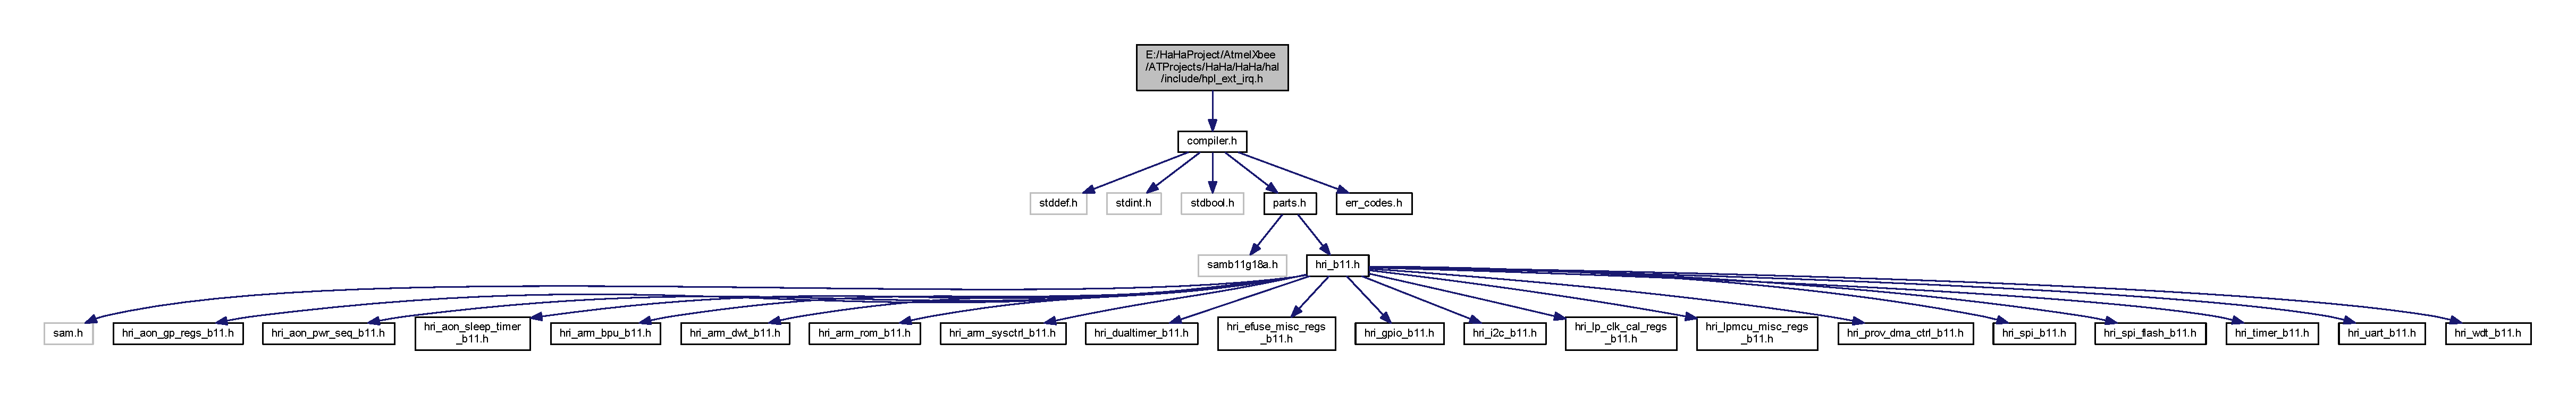
\includegraphics[width=350pt]{hpl__ext__irq_8h__incl}
\end{center}
\end{figure}
\subsection*{Functions}
\begin{Indent}\textbf{ H\+PL functions}\par
\begin{DoxyCompactItemize}
\item 
int32\+\_\+t \hyperlink{group___h_p_l_gad7c12a758c9839e074d1d97d255e09ab}{\+\_\+ext\+\_\+irq\+\_\+init} (void($\ast$cb)(const uint32\+\_\+t pin))
\begin{DoxyCompactList}\small\item\em Initialize external interrupt module. \end{DoxyCompactList}\item 
int32\+\_\+t \hyperlink{group___h_p_l_gad29f685cb658b260303c55fb7a88cdb0}{\+\_\+ext\+\_\+irq\+\_\+deinit} (void)
\begin{DoxyCompactList}\small\item\em Deinitialize external interrupt module. \end{DoxyCompactList}\item 
int32\+\_\+t \hyperlink{group___h_p_l_gac2fa4b43da6356425b0188b744b6f4cc}{\+\_\+ext\+\_\+irq\+\_\+enable} (const uint32\+\_\+t pin, const bool enable)
\begin{DoxyCompactList}\small\item\em Enable / disable external irq. \end{DoxyCompactList}\end{DoxyCompactItemize}
\end{Indent}


\subsection{Detailed Description}
External I\+RQ related functionality declaration. 

Copyright (C) 2015 Atmel Corporation. All rights reserved.
\hypertarget{hpl__gpio_8h}{}\section{E\+:/\+Ha\+Ha\+Project/\+Atmel\+Xbee/\+A\+T\+Projects/\+Ha\+Ha/\+Ha\+Ha/hal/include/hpl\+\_\+gpio.h File Reference}
\label{hpl__gpio_8h}\index{E\+:/\+Ha\+Ha\+Project/\+Atmel\+Xbee/\+A\+T\+Projects/\+Ha\+Ha/\+Ha\+Ha/hal/include/hpl\+\_\+gpio.\+h@{E\+:/\+Ha\+Ha\+Project/\+Atmel\+Xbee/\+A\+T\+Projects/\+Ha\+Ha/\+Ha\+Ha/hal/include/hpl\+\_\+gpio.\+h}}


Port related functionality declaration.  


{\ttfamily \#include $<$compiler.\+h$>$}\newline
{\ttfamily \#include $<$hpl\+\_\+gpio\+\_\+base.\+h$>$}\newline
Include dependency graph for hpl\+\_\+gpio.\+h\+:\nopagebreak
\begin{figure}[H]
\begin{center}
\leavevmode
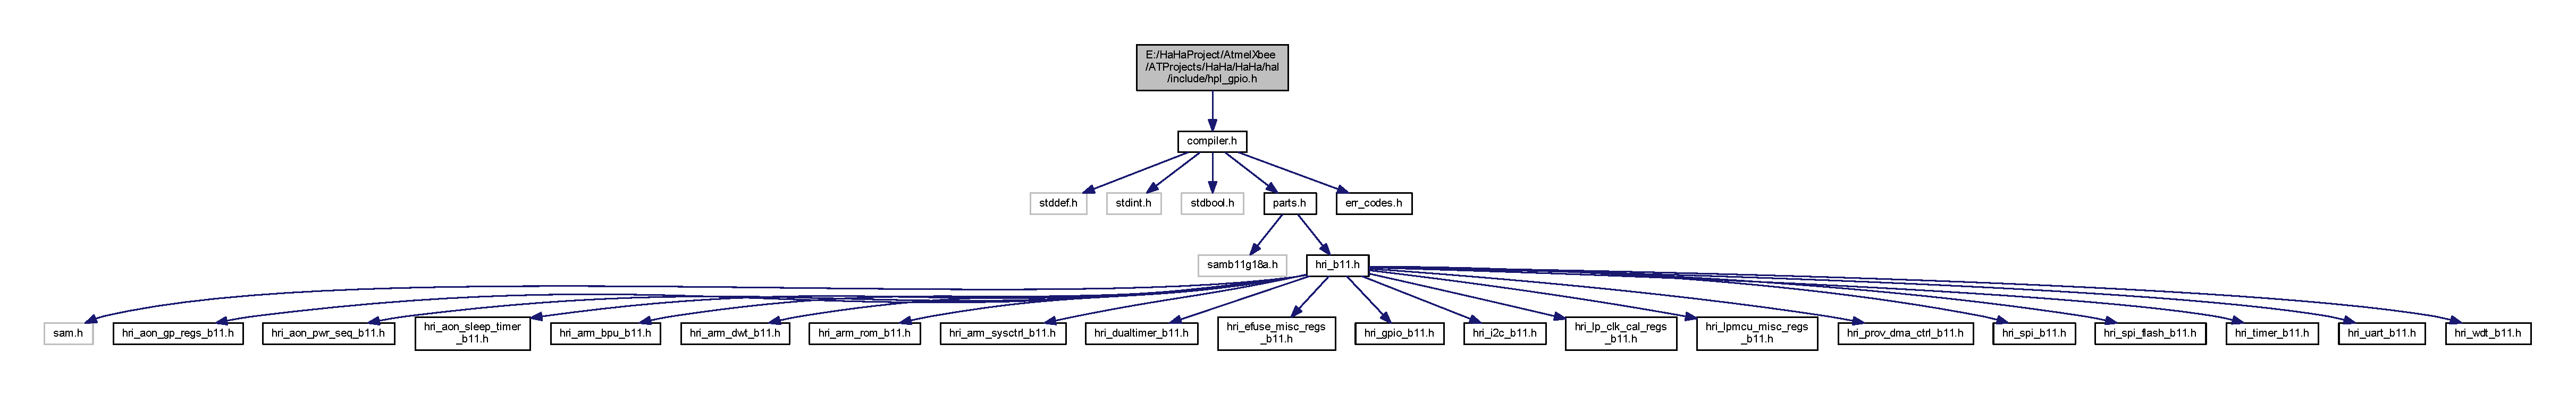
\includegraphics[width=350pt]{hpl__gpio_8h__incl}
\end{center}
\end{figure}
This graph shows which files directly or indirectly include this file\+:\nopagebreak
\begin{figure}[H]
\begin{center}
\leavevmode
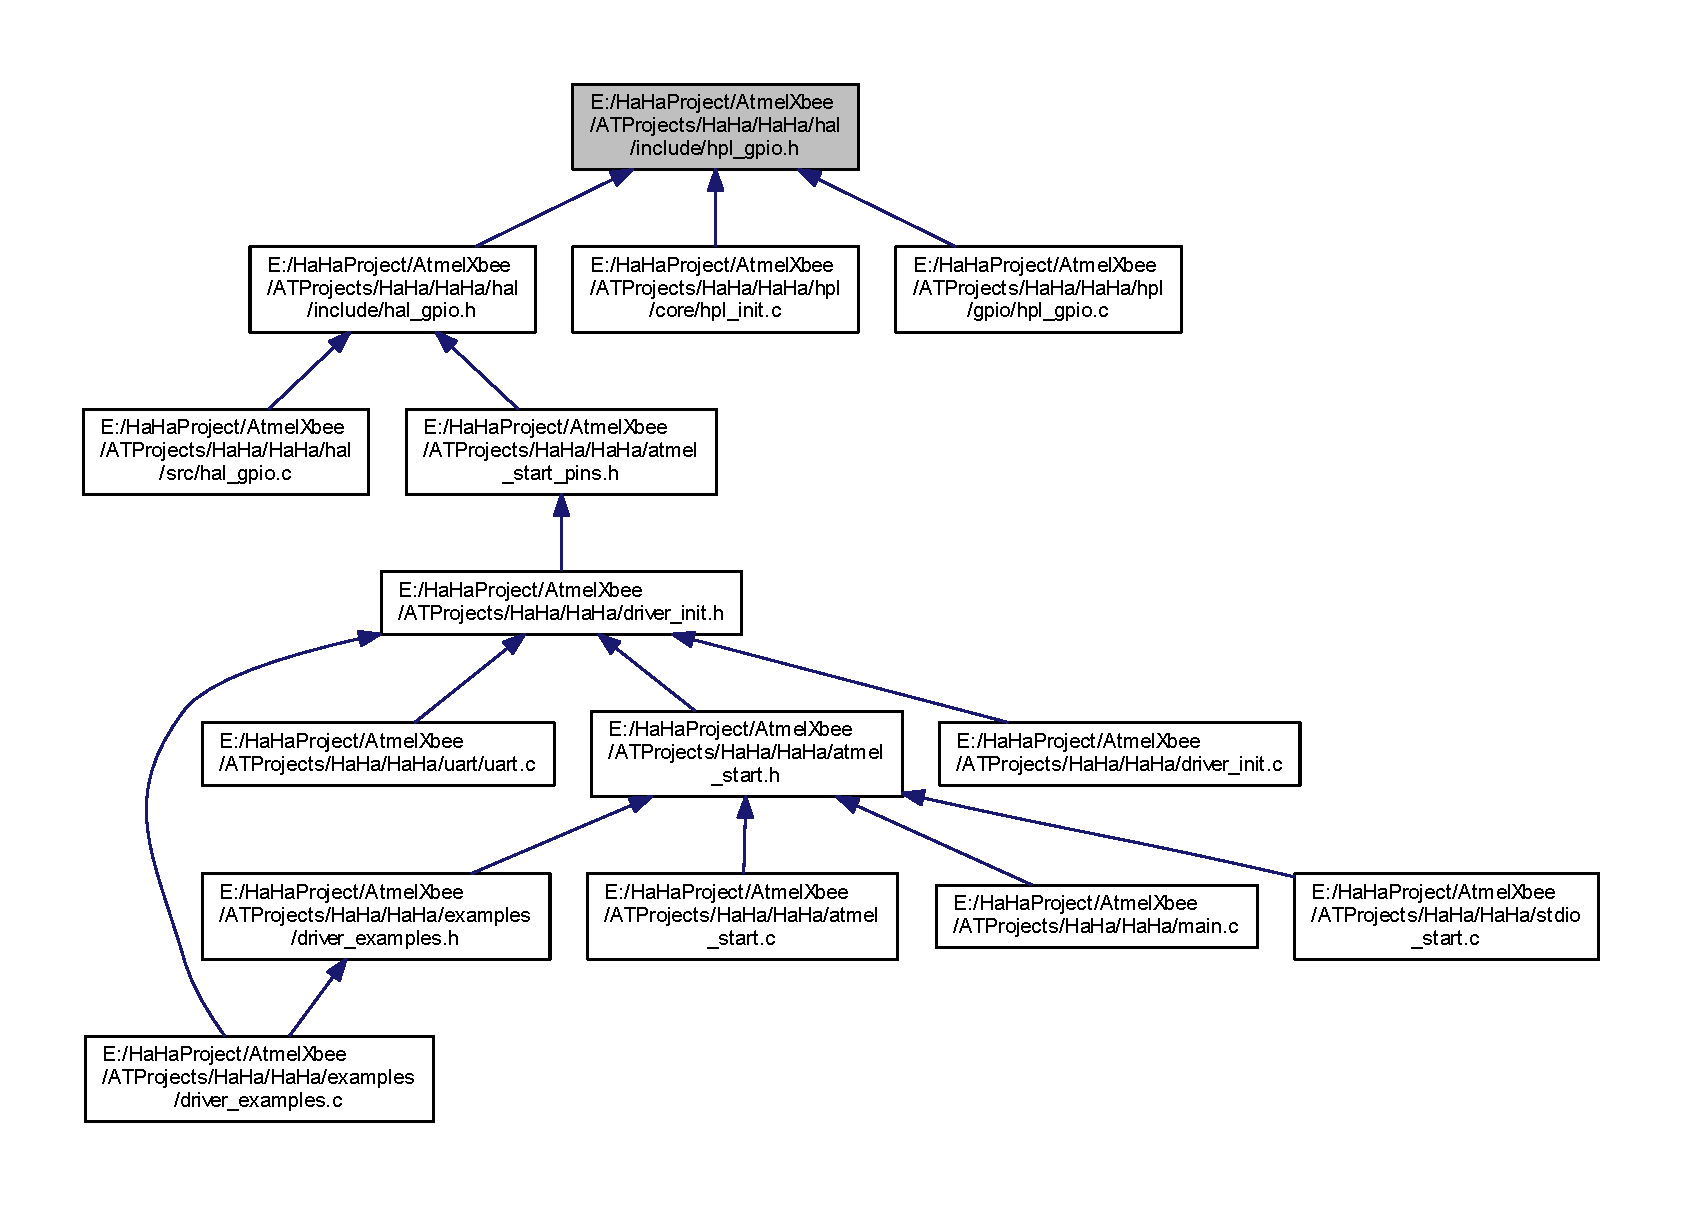
\includegraphics[width=350pt]{hpl__gpio_8h__dep__incl}
\end{center}
\end{figure}
\subsection*{Macros}
\begin{DoxyCompactItemize}
\item 
\#define \hyperlink{group___h_p_l_ga50e2e0aca2b651e066ebc5aeb5fdad25}{G\+P\+I\+O\+\_\+\+P\+IN}(n)~(((n)\&0x1\+Fu) $<$$<$ 0)
\begin{DoxyCompactList}\small\item\em Macros for the pin and port group, lower 5 bits stands for pin number in the group, higher 3 bits stands for port group. \end{DoxyCompactList}\item 
\#define \hyperlink{group___h_p_l_ga9797315af6a0aa3291bb73648a3b1379}{G\+P\+I\+O\+\_\+\+P\+O\+RT}(n)~((n) $>$$>$ 5)
\item 
\#define \hyperlink{group___h_p_l_gaf065b9160b968f60a562bdc5c4454a5a}{G\+P\+IO}(port,  pin)~((((port)\&0x7u) $<$$<$ 5) + ((pin)\&0x1\+Fu))
\item 
\#define \hyperlink{group___h_p_l_ga4ac520942c3dfa92e76b896518718576}{G\+P\+I\+O\+\_\+\+P\+I\+N\+\_\+\+F\+U\+N\+C\+T\+I\+O\+N\+\_\+\+O\+FF}~0xffffffff
\end{DoxyCompactItemize}
\subsection*{Enumerations}
\begin{DoxyCompactItemize}
\item 
enum \hyperlink{group___h_p_l_gab9959d4bcdc5049e5898d5100ada3197}{gpio\+\_\+pull\+\_\+mode} \{ \hyperlink{group___h_p_l_ggab9959d4bcdc5049e5898d5100ada3197a904014efc4ca8e6ab21b5fdf8dead41b}{G\+P\+I\+O\+\_\+\+P\+U\+L\+L\+\_\+\+O\+FF}, 
\hyperlink{group___h_p_l_ggab9959d4bcdc5049e5898d5100ada3197ae7d1b2a9078939dd744dd9a7cd61d9df}{G\+P\+I\+O\+\_\+\+P\+U\+L\+L\+\_\+\+UP}, 
\hyperlink{group___h_p_l_ggab9959d4bcdc5049e5898d5100ada3197a93970a9b4ab92816371682f4e537a8e2}{G\+P\+I\+O\+\_\+\+P\+U\+L\+L\+\_\+\+D\+O\+WN}
 \}\begin{DoxyCompactList}\small\item\em P\+O\+RT pull mode settings. \end{DoxyCompactList}
\item 
enum \hyperlink{group___h_p_l_gaccc7d029df9e5a96151a68e64f4be7e2}{gpio\+\_\+direction} \{ \hyperlink{group___h_p_l_ggaccc7d029df9e5a96151a68e64f4be7e2ae5e30917e4c3b63976e3785711a268f6}{G\+P\+I\+O\+\_\+\+D\+I\+R\+E\+C\+T\+I\+O\+N\+\_\+\+O\+FF}, 
\hyperlink{group___h_p_l_ggaccc7d029df9e5a96151a68e64f4be7e2aea9c54895635603d054830602ba5fb4e}{G\+P\+I\+O\+\_\+\+D\+I\+R\+E\+C\+T\+I\+O\+N\+\_\+\+IN}, 
\hyperlink{group___h_p_l_ggaccc7d029df9e5a96151a68e64f4be7e2a869f710c2bafc06d7ef192861b8358ab}{G\+P\+I\+O\+\_\+\+D\+I\+R\+E\+C\+T\+I\+O\+N\+\_\+\+O\+UT}
 \}\begin{DoxyCompactList}\small\item\em P\+O\+RT direction settins. \end{DoxyCompactList}
\item 
enum \hyperlink{group___h_p_l_ga6d50d8c4b17ff573c07340d4d7965bc1}{gpio\+\_\+port} \{ \newline
\hyperlink{group___h_p_l_gga6d50d8c4b17ff573c07340d4d7965bc1a0d36b47f173bbc4bdced28d8a54fe4ac}{G\+P\+I\+O\+\_\+\+P\+O\+R\+TA}, 
\hyperlink{group___h_p_l_gga6d50d8c4b17ff573c07340d4d7965bc1a258a8ca8e34cedcfba339d2463ae0c2a}{G\+P\+I\+O\+\_\+\+P\+O\+R\+TB}, 
\hyperlink{group___h_p_l_gga6d50d8c4b17ff573c07340d4d7965bc1a3266325667899f8d82c0624c493fda51}{G\+P\+I\+O\+\_\+\+P\+O\+R\+TC}, 
\hyperlink{group___h_p_l_gga6d50d8c4b17ff573c07340d4d7965bc1a4db7e328496cabe7a12e3879f7be8e39}{G\+P\+I\+O\+\_\+\+P\+O\+R\+TD}, 
\newline
\hyperlink{group___h_p_l_gga6d50d8c4b17ff573c07340d4d7965bc1ae00a95999282684e3c5d713937bc74e3}{G\+P\+I\+O\+\_\+\+P\+O\+R\+TE}
 \}\begin{DoxyCompactList}\small\item\em P\+O\+RT group abstraction. \end{DoxyCompactList}
\end{DoxyCompactItemize}
\subsection*{Functions}
\begin{Indent}\textbf{ H\+PL functions}\par
\begin{DoxyCompactItemize}
\item 
void \hyperlink{group___h_p_l_ga6e226919d4a3ee84599b55a32597e284}{\+\_\+gpio\+\_\+init} (void)
\begin{DoxyCompactList}\small\item\em Port initialization function. \end{DoxyCompactList}\end{DoxyCompactItemize}
\end{Indent}


\subsection{Detailed Description}
Port related functionality declaration. 

Copyright (C) 2014-\/2016 Atmel Corporation. All rights reserved.
\hypertarget{hpl__init_8h}{}\section{E\+:/\+Ha\+Ha\+Project/\+Atmel\+Xbee/\+A\+T\+Projects/\+Ha\+Ha/\+Ha\+Ha/hal/include/hpl\+\_\+init.h File Reference}
\label{hpl__init_8h}\index{E\+:/\+Ha\+Ha\+Project/\+Atmel\+Xbee/\+A\+T\+Projects/\+Ha\+Ha/\+Ha\+Ha/hal/include/hpl\+\_\+init.\+h@{E\+:/\+Ha\+Ha\+Project/\+Atmel\+Xbee/\+A\+T\+Projects/\+Ha\+Ha/\+Ha\+Ha/hal/include/hpl\+\_\+init.\+h}}


Init related functionality declaration.  


{\ttfamily \#include $<$compiler.\+h$>$}\newline
\subsection*{Functions}
\begin{Indent}\textbf{ H\+PL functions}\par
\begin{DoxyCompactItemize}
\item 
void \hyperlink{group___h_p_l_ga11bde7accfa853194b32dae4f27bad40}{\+\_\+sysctrl\+\_\+init\+\_\+sources} (void)
\begin{DoxyCompactList}\small\item\em Initializes clock sources. \end{DoxyCompactList}\item 
void \hyperlink{group___h_p_l_ga0e9b9fbf16506f0f6ad8e8b1aa87dc73}{\+\_\+pm\+\_\+init} (void)
\begin{DoxyCompactList}\small\item\em Initializes Power Manager. \end{DoxyCompactList}\item 
void \hyperlink{group___h_p_l_ga87e8c45b05aee8f3b453630134d3483d}{\+\_\+gclk\+\_\+init\+\_\+generators} (void)
\begin{DoxyCompactList}\small\item\em Initialize generators. \end{DoxyCompactList}\item 
void \hyperlink{group___h_p_l_gaab304aa890beb23e3311aaa2c0def527}{\+\_\+osc32kctrl\+\_\+init\+\_\+sources} (void)
\begin{DoxyCompactList}\small\item\em Initialize 32 k\+Hz clock sources. \end{DoxyCompactList}\item 
void \hyperlink{group___h_p_l_gaee0105b1dbc07a2ca23586aa95f49cc7}{\+\_\+oscctrl\+\_\+init\+\_\+sources} (void)
\begin{DoxyCompactList}\small\item\em Initialize clock sources. \end{DoxyCompactList}\item 
void \hyperlink{group___h_p_l_ga3e5e49081818470968093b6e3597ab5f}{\+\_\+sysctrl\+\_\+init\+\_\+referenced\+\_\+generators} (void)
\begin{DoxyCompactList}\small\item\em Initialize clock sources that need input reference clocks. \end{DoxyCompactList}\item 
void \hyperlink{group___h_p_l_ga2e4746bc23999fe1dc7c02aa4e167bfb}{\+\_\+oscctrl\+\_\+init\+\_\+referenced\+\_\+generators} (void)
\begin{DoxyCompactList}\small\item\em Initialize clock sources that need input reference clocks. \end{DoxyCompactList}\item 
void \hyperlink{group___h_p_l_ga840b5c5290dd94e858db4d89259ba3f4}{\+\_\+mclk\+\_\+init} (void)
\begin{DoxyCompactList}\small\item\em Initialize master clock generator. \end{DoxyCompactList}\item 
void \hyperlink{group___h_p_l_ga3dd85007c9fdeed2ffe1166a33dd6519}{\+\_\+lpmcu\+\_\+misc\+\_\+regs\+\_\+init} (void)
\begin{DoxyCompactList}\small\item\em Initialize clock generator. \end{DoxyCompactList}\item 
void \hyperlink{group___h_p_l_ga580e99e942064901ed0f02f5d8789c7a}{\+\_\+pmc\+\_\+init} (void)
\begin{DoxyCompactList}\small\item\em Initialize clock generator. \end{DoxyCompactList}\item 
void \hyperlink{group___h_p_l_ga1668b7fc690ec56e1f3d54d9f3b8e5f2}{\+\_\+set\+\_\+performance\+\_\+level} (const uint8\+\_\+t level)
\begin{DoxyCompactList}\small\item\em Set performance level. \end{DoxyCompactList}\item 
void \hyperlink{group___h_p_l_gac10942d1aec3f0ce14117119db5e9555}{\+\_\+init\+\_\+chip} (void)
\begin{DoxyCompactList}\small\item\em Initialize the chip. \end{DoxyCompactList}\end{DoxyCompactItemize}
\end{Indent}


\subsection{Detailed Description}
Init related functionality declaration. 

Copyright (C) 2014 Atmel Corporation. All rights reserved.
\hypertarget{hpl__irq_8h}{}\section{E\+:/\+Ha\+Ha\+Project/\+Atmel\+Xbee/\+A\+T\+Projects/\+Ha\+Ha/\+Ha\+Ha/hal/include/hpl\+\_\+irq.h File Reference}
\label{hpl__irq_8h}\index{E\+:/\+Ha\+Ha\+Project/\+Atmel\+Xbee/\+A\+T\+Projects/\+Ha\+Ha/\+Ha\+Ha/hal/include/hpl\+\_\+irq.\+h@{E\+:/\+Ha\+Ha\+Project/\+Atmel\+Xbee/\+A\+T\+Projects/\+Ha\+Ha/\+Ha\+Ha/hal/include/hpl\+\_\+irq.\+h}}


I\+RQ related functionality declaration.  


{\ttfamily \#include $<$compiler.\+h$>$}\newline
Include dependency graph for hpl\+\_\+irq.\+h\+:\nopagebreak
\begin{figure}[H]
\begin{center}
\leavevmode
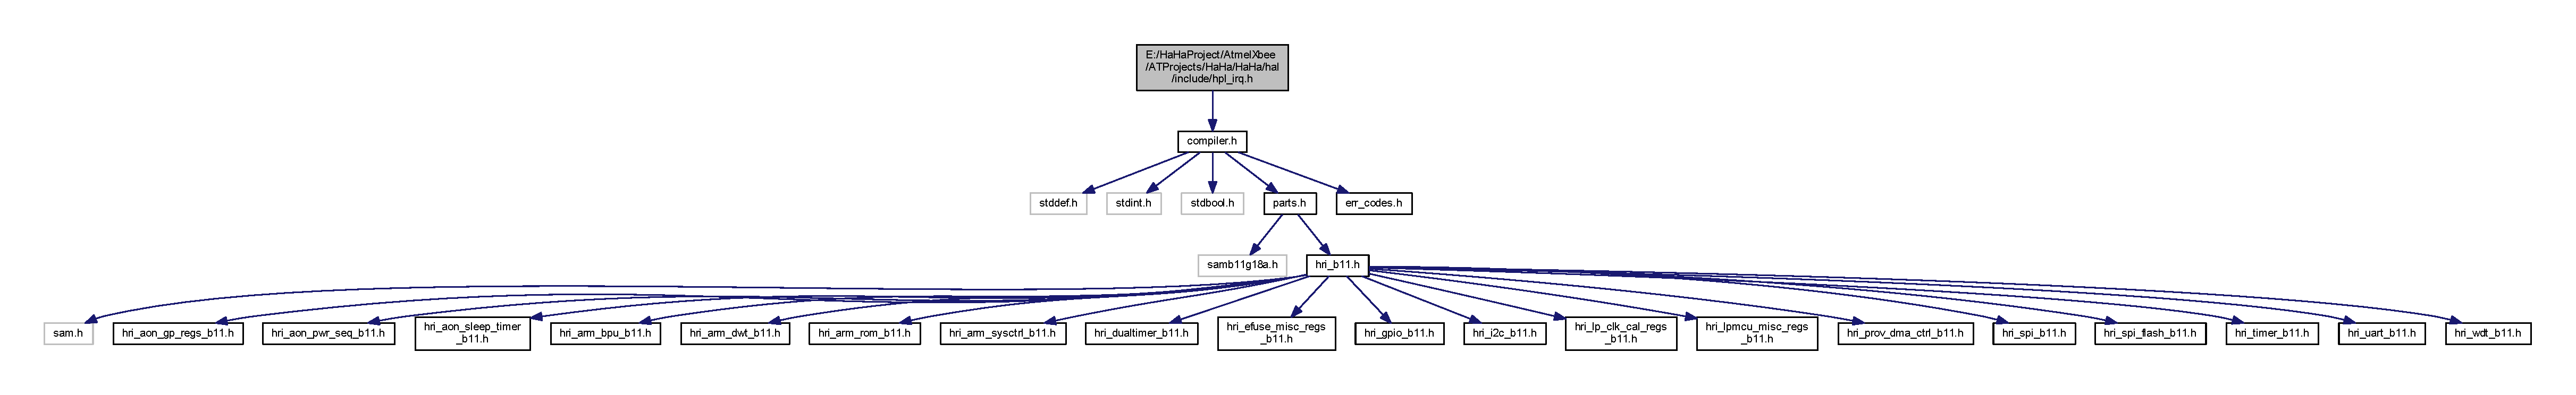
\includegraphics[width=350pt]{hpl__irq_8h__incl}
\end{center}
\end{figure}
This graph shows which files directly or indirectly include this file\+:\nopagebreak
\begin{figure}[H]
\begin{center}
\leavevmode
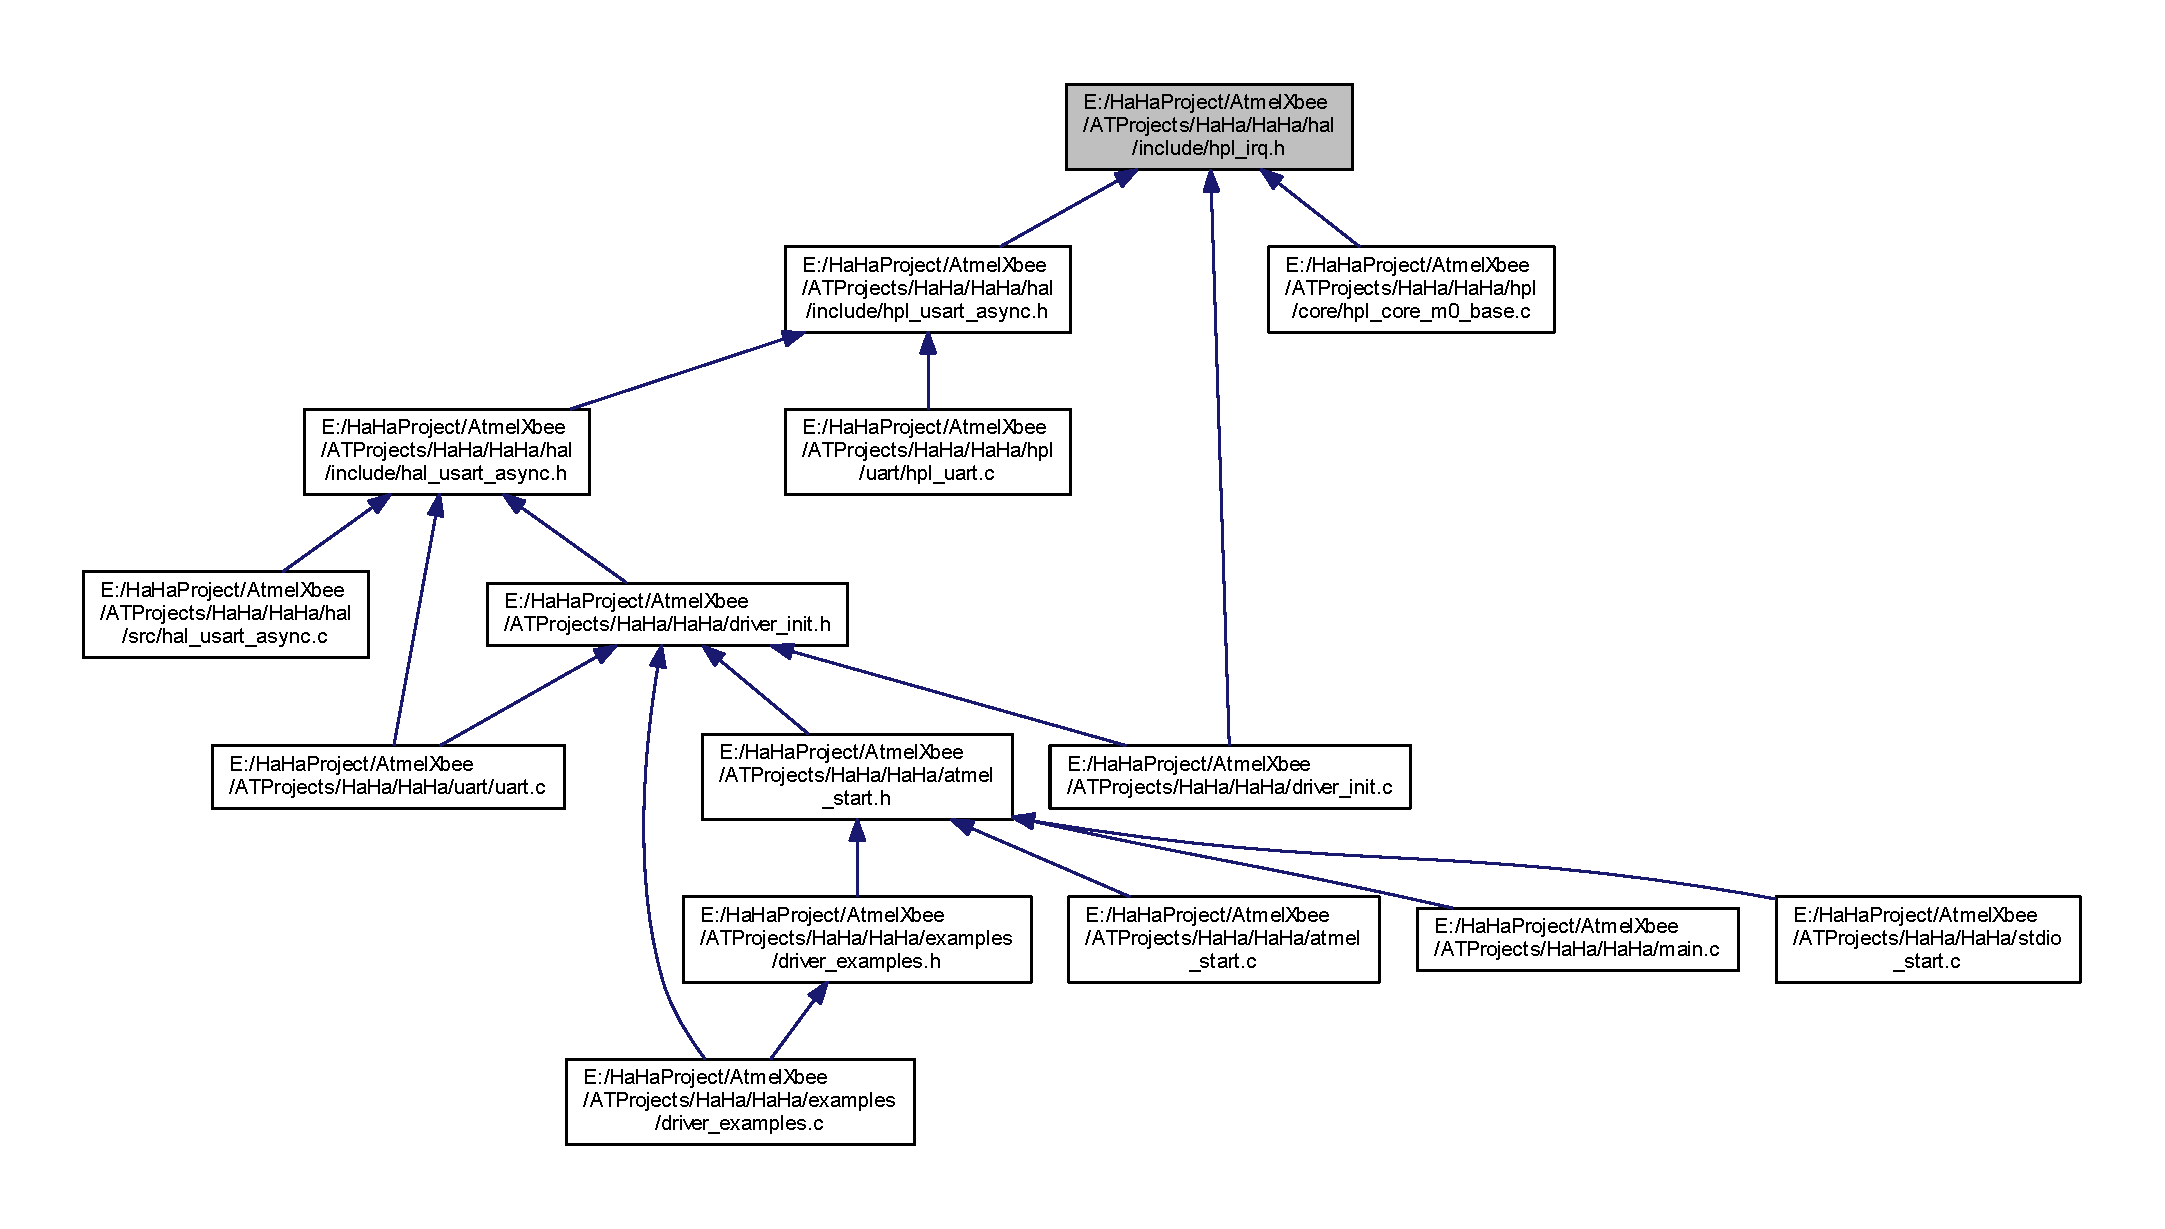
\includegraphics[width=350pt]{hpl__irq_8h__dep__incl}
\end{center}
\end{figure}
\subsection*{Classes}
\begin{DoxyCompactItemize}
\item 
struct \hyperlink{struct__irq__descriptor}{\+\_\+irq\+\_\+descriptor}
\begin{DoxyCompactList}\small\item\em I\+RQ descriptor. \end{DoxyCompactList}\end{DoxyCompactItemize}
\subsection*{Functions}
\begin{Indent}\textbf{ H\+PL functions}\par
\begin{DoxyCompactItemize}
\item 
uint8\+\_\+t \hyperlink{group___h_p_l_ga082e8d19d78ab2cf2f63ded8530c7852}{\+\_\+irq\+\_\+get\+\_\+current} (void)
\begin{DoxyCompactList}\small\item\em Retrieve current I\+RQ number. \end{DoxyCompactList}\item 
void \hyperlink{group___h_p_l_gae6a80cff8a450795dc3f2d6df1a19464}{\+\_\+irq\+\_\+disable} (uint8\+\_\+t n)
\begin{DoxyCompactList}\small\item\em Disable the given I\+RQ. \end{DoxyCompactList}\item 
void \hyperlink{group___h_p_l_ga7720726f19dfdda1561a042483c97a58}{\+\_\+irq\+\_\+set} (uint8\+\_\+t n)
\begin{DoxyCompactList}\small\item\em Set the given I\+RQ. \end{DoxyCompactList}\item 
void \hyperlink{group___h_p_l_ga80f1b1a044a8773e23b38517296620b4}{\+\_\+irq\+\_\+clear} (uint8\+\_\+t n)
\begin{DoxyCompactList}\small\item\em Clear the given I\+RQ. \end{DoxyCompactList}\item 
void \hyperlink{group___h_p_l_gac8b7aa49ad81aecd34603b4dc23dd143}{\+\_\+irq\+\_\+enable} (uint8\+\_\+t n)
\begin{DoxyCompactList}\small\item\em Enable the given I\+RQ. \end{DoxyCompactList}\item 
void \hyperlink{group___h_p_l_ga1ee85f2f8227e335c654b9085e9b7d5c}{\+\_\+irq\+\_\+register} (const uint8\+\_\+t number, struct \hyperlink{struct__irq__descriptor}{\+\_\+irq\+\_\+descriptor} $\ast$const irq)
\begin{DoxyCompactList}\small\item\em Register I\+RQ handler. \end{DoxyCompactList}\end{DoxyCompactItemize}
\end{Indent}


\subsection{Detailed Description}
I\+RQ related functionality declaration. 

Copyright (C) 2014 Atmel Corporation. All rights reserved.
\hypertarget{hpl__missing__features_8h}{}\section{E\+:/\+Ha\+Ha\+Project/\+Atmel\+Xbee/\+A\+T\+Projects/\+Ha\+Ha/\+Ha\+Ha/hal/include/hpl\+\_\+missing\+\_\+features.h File Reference}
\label{hpl__missing__features_8h}\index{E\+:/\+Ha\+Ha\+Project/\+Atmel\+Xbee/\+A\+T\+Projects/\+Ha\+Ha/\+Ha\+Ha/hal/include/hpl\+\_\+missing\+\_\+features.\+h@{E\+:/\+Ha\+Ha\+Project/\+Atmel\+Xbee/\+A\+T\+Projects/\+Ha\+Ha/\+Ha\+Ha/hal/include/hpl\+\_\+missing\+\_\+features.\+h}}


Family-\/dependent missing features expected by H\+AL.  


{\ttfamily \#include \char`\"{}hpl\+\_\+aon\+\_\+gp\+\_\+regs\+\_\+adc\+\_\+missing\+\_\+features.\+h\char`\"{}}\newline
Include dependency graph for hpl\+\_\+missing\+\_\+features.\+h\+:\nopagebreak
\begin{figure}[H]
\begin{center}
\leavevmode
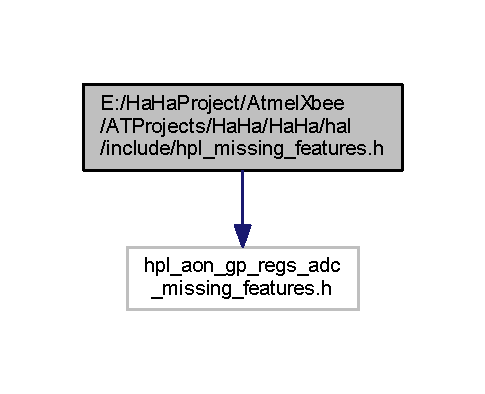
\includegraphics[width=233pt]{hpl__missing__features_8h__incl}
\end{center}
\end{figure}


\subsection{Detailed Description}
Family-\/dependent missing features expected by H\+AL. 

Copyright (C) 2016 Atmel Corporation. All rights reserved.
\hypertarget{hpl__usart_8h}{}\section{E\+:/\+Ha\+Ha\+Project/\+Atmel\+Xbee/\+A\+T\+Projects/\+Ha\+Ha/\+Ha\+Ha/hal/include/hpl\+\_\+usart.h File Reference}
\label{hpl__usart_8h}\index{E\+:/\+Ha\+Ha\+Project/\+Atmel\+Xbee/\+A\+T\+Projects/\+Ha\+Ha/\+Ha\+Ha/hal/include/hpl\+\_\+usart.\+h@{E\+:/\+Ha\+Ha\+Project/\+Atmel\+Xbee/\+A\+T\+Projects/\+Ha\+Ha/\+Ha\+Ha/hal/include/hpl\+\_\+usart.\+h}}


U\+S\+A\+RT related functionality declaration.  


{\ttfamily \#include $<$compiler.\+h$>$}\newline
Include dependency graph for hpl\+\_\+usart.\+h\+:\nopagebreak
\begin{figure}[H]
\begin{center}
\leavevmode
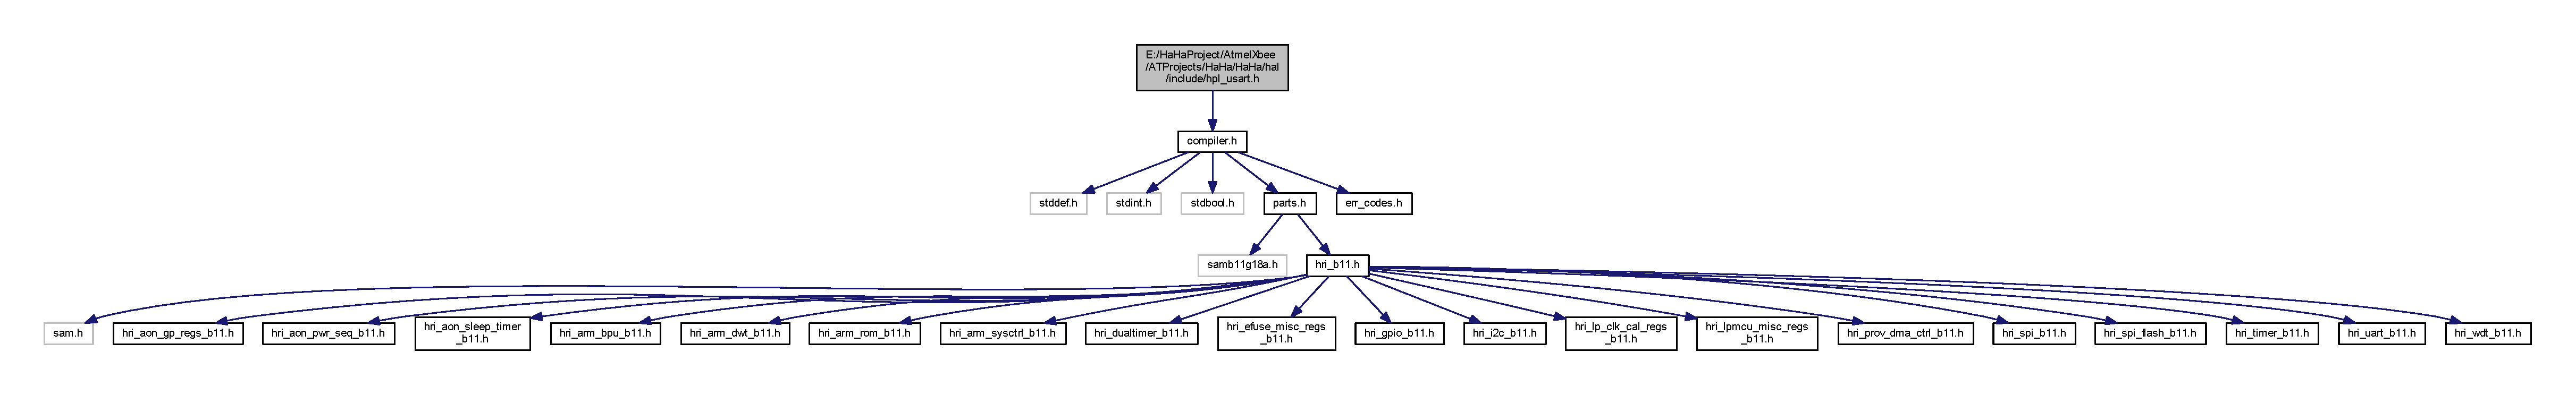
\includegraphics[width=350pt]{hpl__usart_8h__incl}
\end{center}
\end{figure}
This graph shows which files directly or indirectly include this file\+:\nopagebreak
\begin{figure}[H]
\begin{center}
\leavevmode
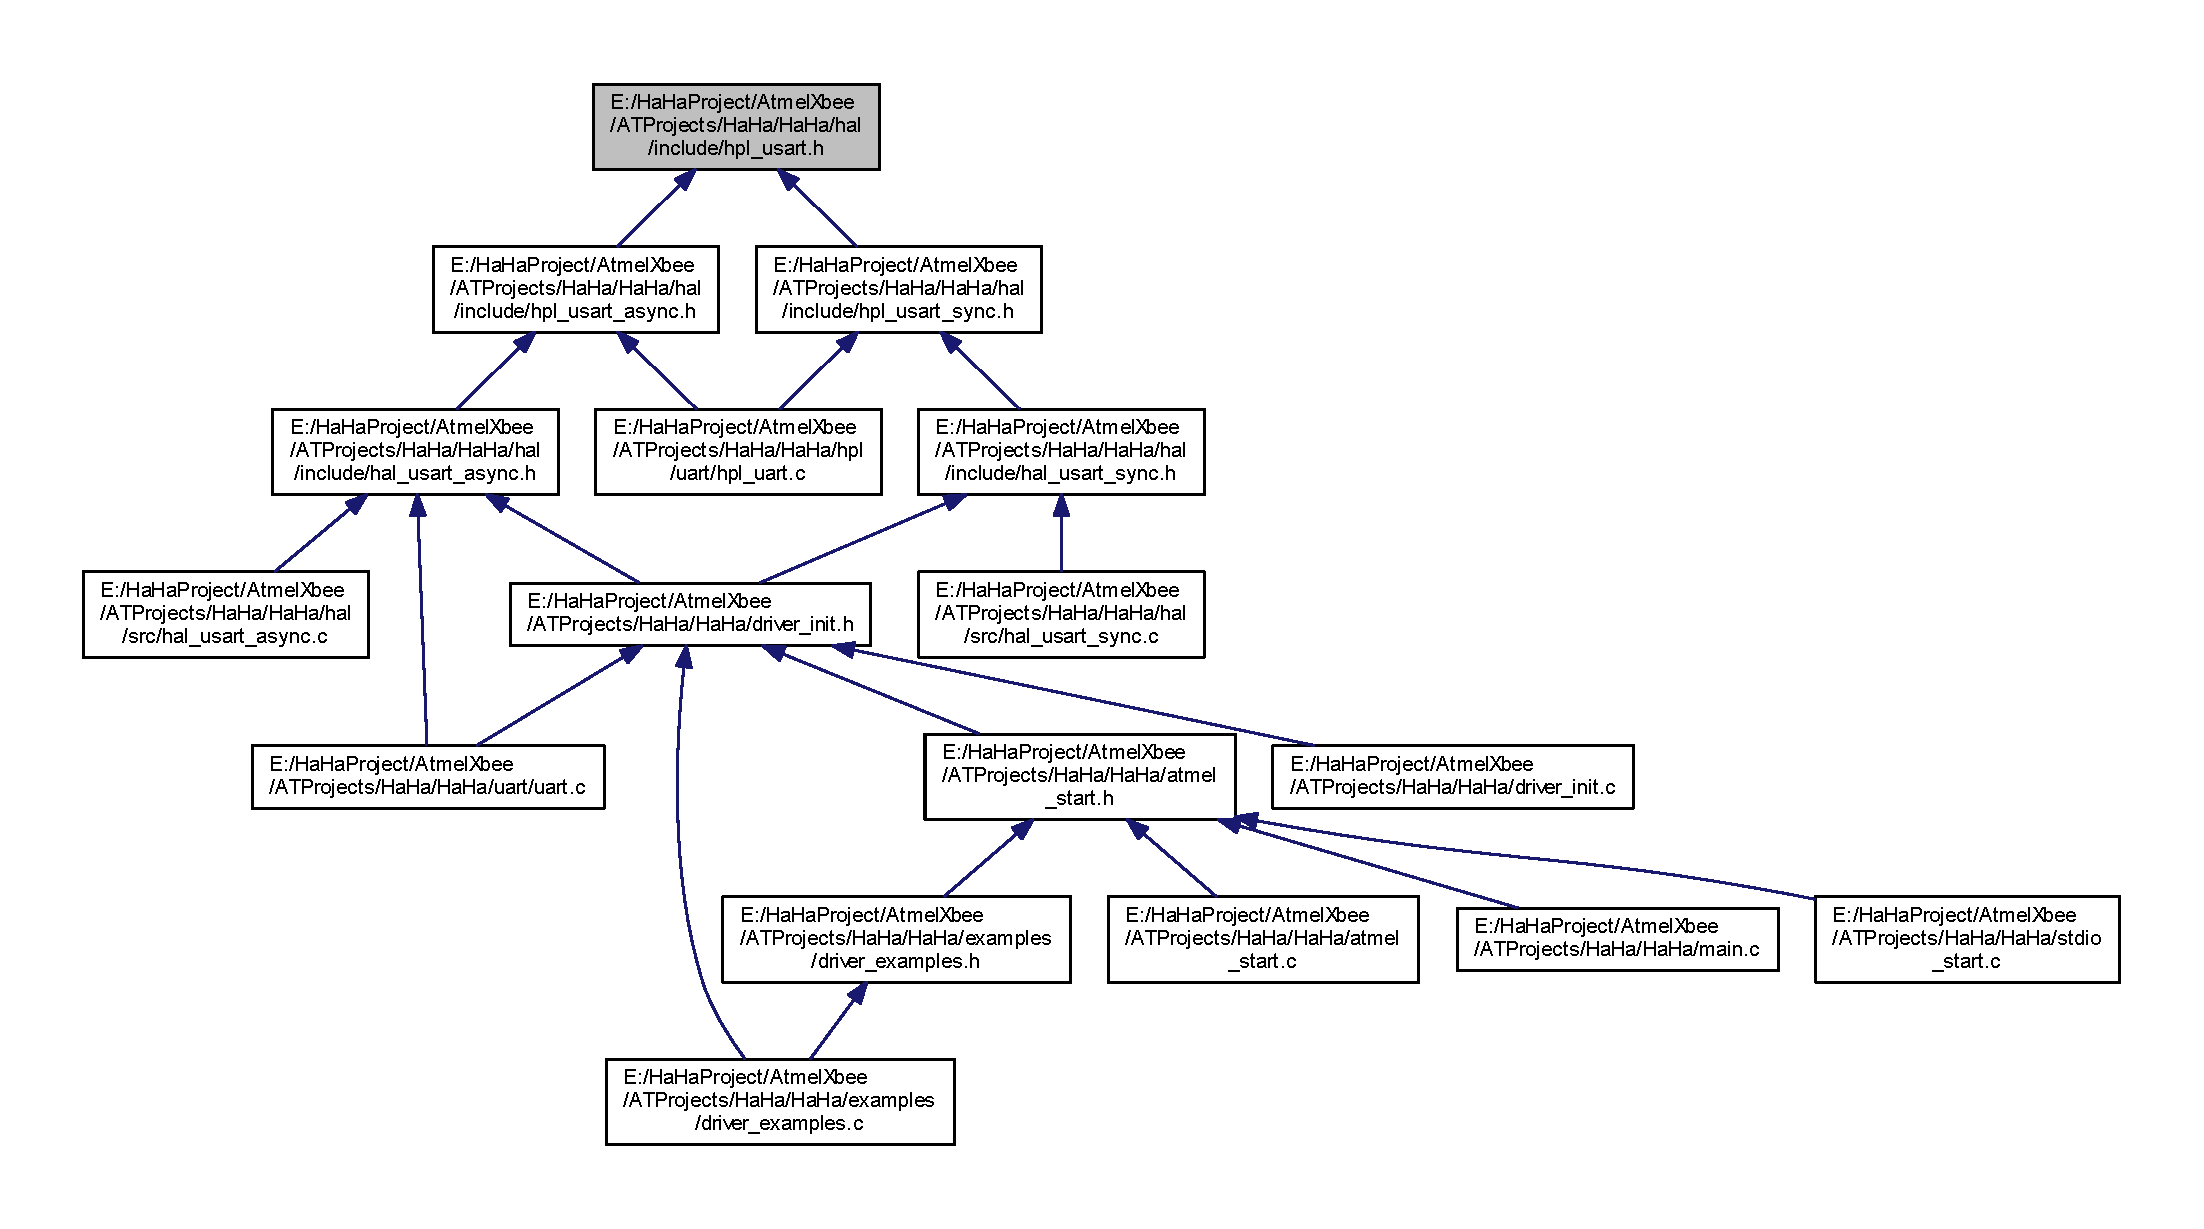
\includegraphics[width=350pt]{hpl__usart_8h__dep__incl}
\end{center}
\end{figure}
\subsection*{Classes}
\begin{DoxyCompactItemize}
\item 
union \hyperlink{unionusart__flow__control__state}{usart\+\_\+flow\+\_\+control\+\_\+state}
\begin{DoxyCompactList}\small\item\em U\+S\+A\+RT flow control state. \end{DoxyCompactList}\end{DoxyCompactItemize}
\subsection*{Enumerations}
\begin{DoxyCompactItemize}
\item 
enum \hyperlink{group___h_p_l_ga59141b5eb86f4d53f17bbeab1d7c83e7}{usart\+\_\+baud\+\_\+rate\+\_\+mode} \{ \hyperlink{group___h_p_l_gga59141b5eb86f4d53f17bbeab1d7c83e7a9dfbfc309d416d0a7133146b967aff12}{U\+S\+A\+R\+T\+\_\+\+B\+A\+U\+D\+R\+A\+T\+E\+\_\+\+A\+S\+Y\+N\+C\+H\+\_\+\+A\+R\+I\+T\+H\+M\+E\+T\+IC}, 
\hyperlink{group___h_p_l_gga59141b5eb86f4d53f17bbeab1d7c83e7a88eeba612b4bb837118d0b58fb362154}{U\+S\+A\+R\+T\+\_\+\+B\+A\+U\+D\+R\+A\+T\+E\+\_\+\+A\+S\+Y\+N\+C\+H\+\_\+\+F\+R\+A\+C\+T\+I\+O\+N\+AL}, 
\hyperlink{group___h_p_l_gga59141b5eb86f4d53f17bbeab1d7c83e7a6ea0c41087b56d5b6111bc75c7fa4fce}{U\+S\+A\+R\+T\+\_\+\+B\+A\+U\+D\+R\+A\+T\+E\+\_\+\+S\+Y\+N\+CH}
 \}\begin{DoxyCompactList}\small\item\em U\+S\+A\+RT baud rate mode. \end{DoxyCompactList}
\item 
enum \hyperlink{group___h_p_l_ga426849bbd9655cec091101ebc9123eb4}{usart\+\_\+data\+\_\+order} \{ \hyperlink{group___h_p_l_gga426849bbd9655cec091101ebc9123eb4afd8bb97c0b2a548d9e3cb9b55e78c4bd}{U\+S\+A\+R\+T\+\_\+\+D\+A\+T\+A\+\_\+\+O\+R\+D\+E\+R\+\_\+\+M\+SB} = 0, 
\hyperlink{group___h_p_l_gga426849bbd9655cec091101ebc9123eb4a88ca2528623acb9433729123f12f5518}{U\+S\+A\+R\+T\+\_\+\+D\+A\+T\+A\+\_\+\+O\+R\+D\+E\+R\+\_\+\+L\+SB} = 1
 \}\begin{DoxyCompactList}\small\item\em U\+S\+A\+RT data order. \end{DoxyCompactList}
\item 
enum \hyperlink{group___h_p_l_ga1c465965478e0f6908a4c99d4f3ad20f}{usart\+\_\+mode} \{ \hyperlink{group___h_p_l_gga1c465965478e0f6908a4c99d4f3ad20fa15ae875c7e7097405cb441a311d6a4d8}{U\+S\+A\+R\+T\+\_\+\+M\+O\+D\+E\+\_\+\+A\+S\+Y\+N\+C\+H\+R\+O\+N\+O\+US} = 0, 
\hyperlink{group___h_p_l_gga1c465965478e0f6908a4c99d4f3ad20fa004992ac327040dfff2102581111a7e9}{U\+S\+A\+R\+T\+\_\+\+M\+O\+D\+E\+\_\+\+S\+Y\+N\+C\+H\+R\+O\+N\+O\+US} = 1
 \}\begin{DoxyCompactList}\small\item\em U\+S\+A\+RT mode. \end{DoxyCompactList}
\item 
enum \hyperlink{group___h_p_l_ga867cc5f0ea7d3bf651d68f0046cf6f41}{usart\+\_\+parity} \{ \newline
\hyperlink{group___h_p_l_gga867cc5f0ea7d3bf651d68f0046cf6f41ae5d22c99a30184aff19d77c1a970fb23}{U\+S\+A\+R\+T\+\_\+\+P\+A\+R\+I\+T\+Y\+\_\+\+E\+V\+EN} = 0, 
\hyperlink{group___h_p_l_gga867cc5f0ea7d3bf651d68f0046cf6f41a69c6cdd4d354d3b26c8d2f09f49d2ede}{U\+S\+A\+R\+T\+\_\+\+P\+A\+R\+I\+T\+Y\+\_\+\+O\+DD} = 1, 
\hyperlink{group___h_p_l_gga867cc5f0ea7d3bf651d68f0046cf6f41aecf52ec650226bdc63e12a21d3b5585d}{U\+S\+A\+R\+T\+\_\+\+P\+A\+R\+I\+T\+Y\+\_\+\+N\+O\+NE} = 2, 
\hyperlink{group___h_p_l_gga867cc5f0ea7d3bf651d68f0046cf6f41a67f8ec9a06b6c88969caae8b186a680a}{U\+S\+A\+R\+T\+\_\+\+P\+A\+R\+I\+T\+Y\+\_\+\+S\+P\+A\+CE} = 3, 
\newline
\hyperlink{group___h_p_l_gga867cc5f0ea7d3bf651d68f0046cf6f41adaac8e86191a3f82a0da0610bacff70d}{U\+S\+A\+R\+T\+\_\+\+P\+A\+R\+I\+T\+Y\+\_\+\+M\+A\+RK} = 4
 \}\begin{DoxyCompactList}\small\item\em U\+S\+A\+RT parity. \end{DoxyCompactList}
\item 
enum \hyperlink{group___h_p_l_ga88311517c5168c29a681604a8a33b06e}{usart\+\_\+stop\+\_\+bits} \{ \hyperlink{group___h_p_l_gga88311517c5168c29a681604a8a33b06ea6353d11d2e690bbaed6572dd1e2d6515}{U\+S\+A\+R\+T\+\_\+\+S\+T\+O\+P\+\_\+\+B\+I\+T\+S\+\_\+\+O\+NE} = 0, 
\hyperlink{group___h_p_l_gga88311517c5168c29a681604a8a33b06ea1b705e4ff84a8839ffffdf2929772366}{U\+S\+A\+R\+T\+\_\+\+S\+T\+O\+P\+\_\+\+B\+I\+T\+S\+\_\+\+T\+WO} = 1, 
\hyperlink{group___h_p_l_gga88311517c5168c29a681604a8a33b06ea09d207bc4b627981d32fff8b0ed235f8}{U\+S\+A\+R\+T\+\_\+\+S\+T\+O\+P\+\_\+\+B\+I\+T\+S\+\_\+\+O\+N\+E\+\_\+\+P\+\_\+\+F\+I\+VE} = 2
 \}\begin{DoxyCompactList}\small\item\em U\+S\+A\+RT stop bits mode. \end{DoxyCompactList}
\item 
enum \hyperlink{group___h_p_l_ga631ce7b4f60dccd392e6d6ef7d3cd4e2}{usart\+\_\+character\+\_\+size} \{ \newline
\hyperlink{group___h_p_l_gga631ce7b4f60dccd392e6d6ef7d3cd4e2ad7d75e6dd09ada4e328e9d77ea5a882a}{U\+S\+A\+R\+T\+\_\+\+C\+H\+A\+R\+A\+C\+T\+E\+R\+\_\+\+S\+I\+Z\+E\+\_\+8\+B\+I\+TS} = 0, 
\hyperlink{group___h_p_l_gga631ce7b4f60dccd392e6d6ef7d3cd4e2a8a0da561e5c3c43da6e334e5a7d9d363}{U\+S\+A\+R\+T\+\_\+\+C\+H\+A\+R\+A\+C\+T\+E\+R\+\_\+\+S\+I\+Z\+E\+\_\+9\+B\+I\+TS} = 1, 
\hyperlink{group___h_p_l_gga631ce7b4f60dccd392e6d6ef7d3cd4e2a9d494ae2bc870cd5a4a3e832e3b0334d}{U\+S\+A\+R\+T\+\_\+\+C\+H\+A\+R\+A\+C\+T\+E\+R\+\_\+\+S\+I\+Z\+E\+\_\+5\+B\+I\+TS} = 5, 
\hyperlink{group___h_p_l_gga631ce7b4f60dccd392e6d6ef7d3cd4e2ad8f2a75feeac704acc0b9af6947e4734}{U\+S\+A\+R\+T\+\_\+\+C\+H\+A\+R\+A\+C\+T\+E\+R\+\_\+\+S\+I\+Z\+E\+\_\+6\+B\+I\+TS} = 6, 
\newline
\hyperlink{group___h_p_l_gga631ce7b4f60dccd392e6d6ef7d3cd4e2a9fe87d41d9dd672038c67eaea63d6d96}{U\+S\+A\+R\+T\+\_\+\+C\+H\+A\+R\+A\+C\+T\+E\+R\+\_\+\+S\+I\+Z\+E\+\_\+7\+B\+I\+TS} = 7
 \}\begin{DoxyCompactList}\small\item\em U\+S\+A\+RT character size. \end{DoxyCompactList}
\end{DoxyCompactItemize}


\subsection{Detailed Description}
U\+S\+A\+RT related functionality declaration. 

Copyright (C) 2014 Atmel Corporation. All rights reserved.
\hypertarget{hpl__usart__async_8h}{}\section{E\+:/\+Ha\+Ha\+Project/\+Atmel\+Xbee/\+A\+T\+Projects/\+Ha\+Ha/\+Ha\+Ha/hal/include/hpl\+\_\+usart\+\_\+async.h File Reference}
\label{hpl__usart__async_8h}\index{E\+:/\+Ha\+Ha\+Project/\+Atmel\+Xbee/\+A\+T\+Projects/\+Ha\+Ha/\+Ha\+Ha/hal/include/hpl\+\_\+usart\+\_\+async.\+h@{E\+:/\+Ha\+Ha\+Project/\+Atmel\+Xbee/\+A\+T\+Projects/\+Ha\+Ha/\+Ha\+Ha/hal/include/hpl\+\_\+usart\+\_\+async.\+h}}


U\+S\+A\+RT related functionality declaration.  


{\ttfamily \#include \char`\"{}hpl\+\_\+usart.\+h\char`\"{}}\newline
{\ttfamily \#include \char`\"{}hpl\+\_\+irq.\+h\char`\"{}}\newline
Include dependency graph for hpl\+\_\+usart\+\_\+async.\+h\+:\nopagebreak
\begin{figure}[H]
\begin{center}
\leavevmode
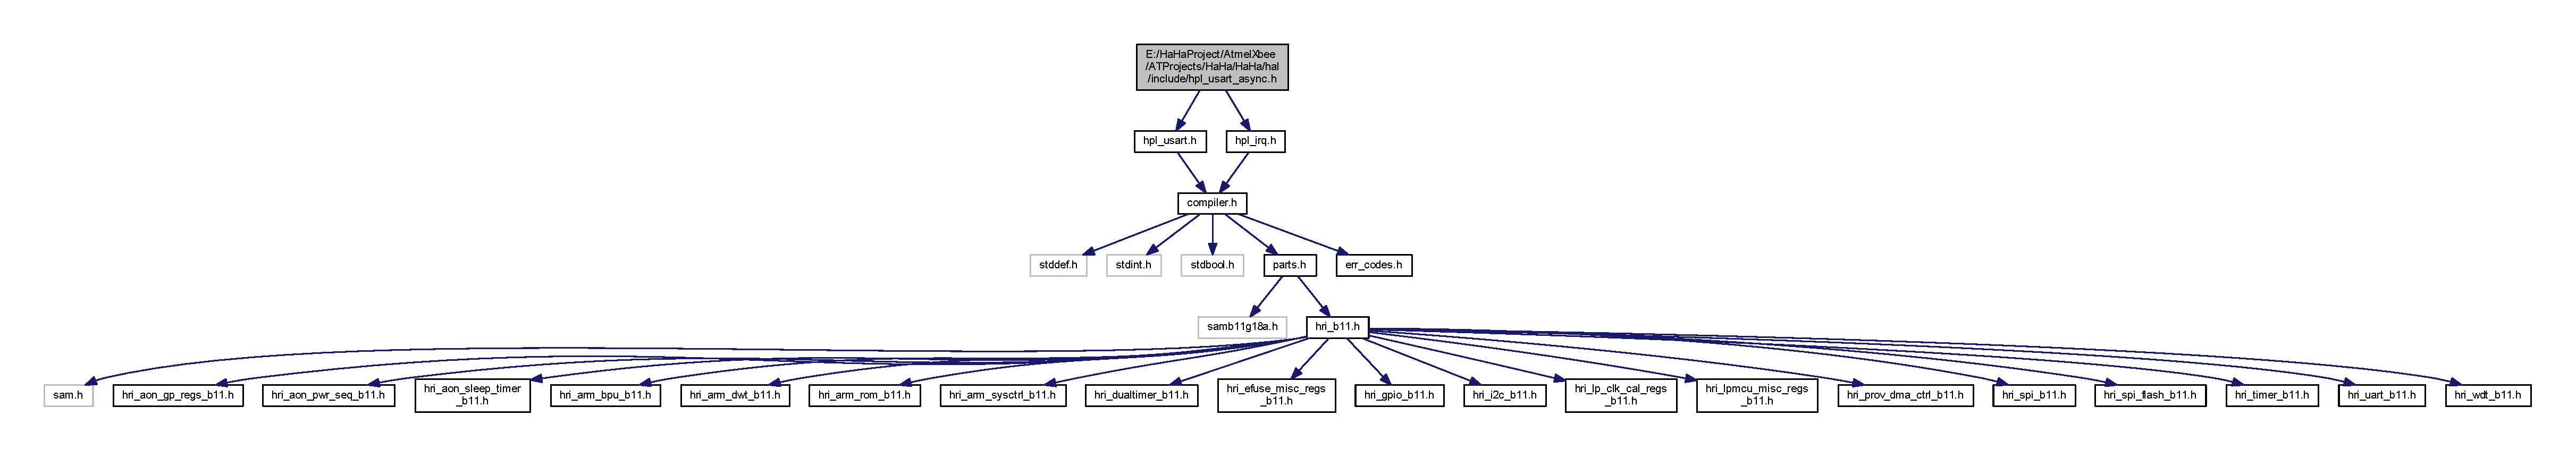
\includegraphics[width=350pt]{hpl__usart__async_8h__incl}
\end{center}
\end{figure}
This graph shows which files directly or indirectly include this file\+:\nopagebreak
\begin{figure}[H]
\begin{center}
\leavevmode
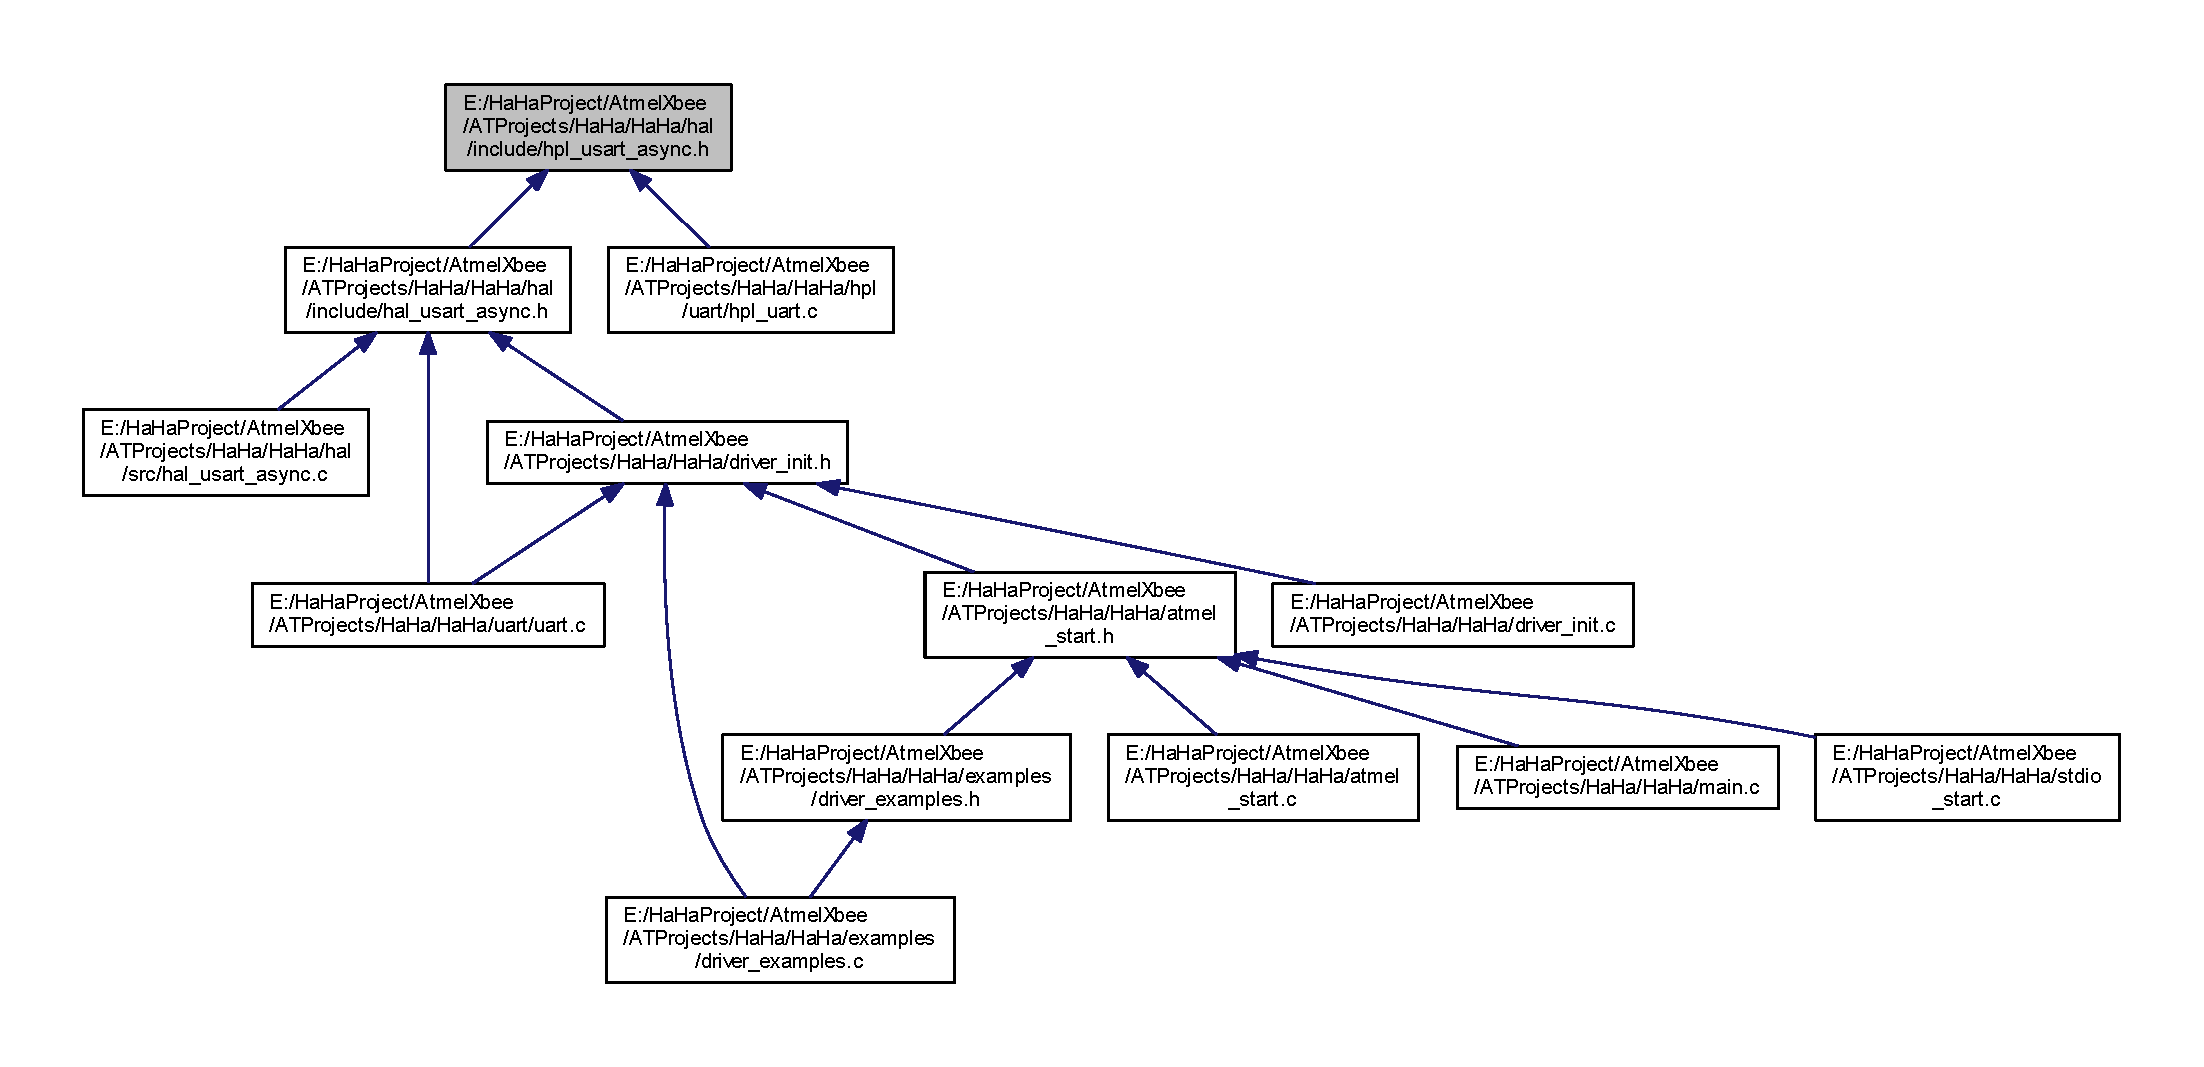
\includegraphics[width=350pt]{hpl__usart__async_8h__dep__incl}
\end{center}
\end{figure}
\subsection*{Classes}
\begin{DoxyCompactItemize}
\item 
struct \hyperlink{struct__usart__async__callbacks}{\+\_\+usart\+\_\+async\+\_\+callbacks}
\begin{DoxyCompactList}\small\item\em U\+S\+A\+RT interrupt callbacks. \end{DoxyCompactList}\item 
struct \hyperlink{struct__usart__async__device}{\+\_\+usart\+\_\+async\+\_\+device}
\begin{DoxyCompactList}\small\item\em U\+S\+A\+RT descriptor device structure. \end{DoxyCompactList}\end{DoxyCompactItemize}
\subsection*{Enumerations}
\begin{DoxyCompactItemize}
\item 
enum \hyperlink{group___h_p_l_gace00dc77ac02c91f8bf35551b484927c}{\+\_\+usart\+\_\+async\+\_\+callback\+\_\+type} \{ \hyperlink{group___h_p_l_ggace00dc77ac02c91f8bf35551b484927ca5cbff5ce7030edf0c23f4e2291839142}{U\+S\+A\+R\+T\+\_\+\+A\+S\+Y\+N\+C\+\_\+\+B\+Y\+T\+E\+\_\+\+S\+E\+NT}, 
\hyperlink{group___h_p_l_ggace00dc77ac02c91f8bf35551b484927cad2ef0bf5b401a3c576c17cab2a6df7bf}{U\+S\+A\+R\+T\+\_\+\+A\+S\+Y\+N\+C\+\_\+\+R\+X\+\_\+\+D\+O\+NE}, 
\hyperlink{group___h_p_l_ggace00dc77ac02c91f8bf35551b484927ca8a94d01c89c71f1bf2a1b68edadbfbfa}{U\+S\+A\+R\+T\+\_\+\+A\+S\+Y\+N\+C\+\_\+\+T\+X\+\_\+\+D\+O\+NE}, 
\hyperlink{group___h_p_l_ggace00dc77ac02c91f8bf35551b484927cac9790dc229a5fa436d2ef48e8ac1024c}{U\+S\+A\+R\+T\+\_\+\+A\+S\+Y\+N\+C\+\_\+\+E\+R\+R\+OR}
 \}\begin{DoxyCompactList}\small\item\em U\+S\+A\+RT callback types. \end{DoxyCompactList}
\end{DoxyCompactItemize}
\subsection*{Functions}
\begin{Indent}\textbf{ H\+PL functions}\par
\begin{DoxyCompactItemize}
\item 
int32\+\_\+t \hyperlink{group___h_p_l_ga11745e0bd0c9d636afbefae8e209665e}{\+\_\+usart\+\_\+async\+\_\+init} (struct \hyperlink{struct__usart__async__device}{\+\_\+usart\+\_\+async\+\_\+device} $\ast$const device, void $\ast$const hw)
\begin{DoxyCompactList}\small\item\em Initialize asynchronous U\+S\+A\+RT. \end{DoxyCompactList}\item 
void \hyperlink{group___h_p_l_ga57e2ef9f6ec11c53a9d88bdb7a82aac4}{\+\_\+usart\+\_\+async\+\_\+deinit} (struct \hyperlink{struct__usart__async__device}{\+\_\+usart\+\_\+async\+\_\+device} $\ast$const device)
\begin{DoxyCompactList}\small\item\em Deinitialize U\+S\+A\+RT. \end{DoxyCompactList}\item 
void \hyperlink{group___h_p_l_ga86c4101798d9dbc584f1e56615140d6f}{\+\_\+usart\+\_\+async\+\_\+enable} (struct \hyperlink{struct__usart__async__device}{\+\_\+usart\+\_\+async\+\_\+device} $\ast$const device)
\begin{DoxyCompactList}\small\item\em Enable usart module. \end{DoxyCompactList}\item 
void \hyperlink{group___h_p_l_gadb6751e5c270eb88eb754f45e7b8a91f}{\+\_\+usart\+\_\+async\+\_\+disable} (struct \hyperlink{struct__usart__async__device}{\+\_\+usart\+\_\+async\+\_\+device} $\ast$const device)
\begin{DoxyCompactList}\small\item\em Disable usart module. \end{DoxyCompactList}\item 
uint16\+\_\+t \hyperlink{group___h_p_l_gab834a3310b05b1118ac7cf5ad90835ba}{\+\_\+usart\+\_\+async\+\_\+calculate\+\_\+baud\+\_\+rate} (const uint32\+\_\+t baud, const uint32\+\_\+t clock\+\_\+rate, const uint8\+\_\+t samples, const enum \hyperlink{group___h_p_l_ga59141b5eb86f4d53f17bbeab1d7c83e7}{usart\+\_\+baud\+\_\+rate\+\_\+mode} mode, const uint8\+\_\+t fraction)
\begin{DoxyCompactList}\small\item\em Calculate baud rate register value. \end{DoxyCompactList}\item 
void \hyperlink{group___h_p_l_gab3211a57f9d6f2e355db5b67ce3fe905}{\+\_\+usart\+\_\+async\+\_\+set\+\_\+baud\+\_\+rate} (struct \hyperlink{struct__usart__async__device}{\+\_\+usart\+\_\+async\+\_\+device} $\ast$const device, const uint32\+\_\+t baud\+\_\+rate)
\begin{DoxyCompactList}\small\item\em Set baud rate. \end{DoxyCompactList}\item 
void \hyperlink{group___h_p_l_ga8f29c61bfbc9298ba0e25be2980ddd15}{\+\_\+usart\+\_\+async\+\_\+set\+\_\+data\+\_\+order} (struct \hyperlink{struct__usart__async__device}{\+\_\+usart\+\_\+async\+\_\+device} $\ast$const device, const enum \hyperlink{group___h_p_l_ga426849bbd9655cec091101ebc9123eb4}{usart\+\_\+data\+\_\+order} order)
\begin{DoxyCompactList}\small\item\em Set data order. \end{DoxyCompactList}\item 
void \hyperlink{group___h_p_l_ga90f1288d1ba0ab800801db3124f6a1cc}{\+\_\+usart\+\_\+async\+\_\+set\+\_\+mode} (struct \hyperlink{struct__usart__async__device}{\+\_\+usart\+\_\+async\+\_\+device} $\ast$const device, const enum \hyperlink{group___h_p_l_ga1c465965478e0f6908a4c99d4f3ad20f}{usart\+\_\+mode} mode)
\begin{DoxyCompactList}\small\item\em Set mode. \end{DoxyCompactList}\item 
void \hyperlink{group___h_p_l_ga739cdfde316390a089c38355bc4f596e}{\+\_\+usart\+\_\+async\+\_\+set\+\_\+parity} (struct \hyperlink{struct__usart__async__device}{\+\_\+usart\+\_\+async\+\_\+device} $\ast$const device, const enum \hyperlink{group___h_p_l_ga867cc5f0ea7d3bf651d68f0046cf6f41}{usart\+\_\+parity} parity)
\begin{DoxyCompactList}\small\item\em Set parity. \end{DoxyCompactList}\item 
void \hyperlink{group___h_p_l_ga7f2ef73e4b9da5be12fc0eabb97ab67b}{\+\_\+usart\+\_\+async\+\_\+set\+\_\+stop\+\_\+bits} (struct \hyperlink{struct__usart__async__device}{\+\_\+usart\+\_\+async\+\_\+device} $\ast$const device, const enum \hyperlink{group___h_p_l_ga88311517c5168c29a681604a8a33b06e}{usart\+\_\+stop\+\_\+bits} stop\+\_\+bits)
\begin{DoxyCompactList}\small\item\em Set stop bits mode. \end{DoxyCompactList}\item 
void \hyperlink{group___h_p_l_gaf834af5cc0738976ddbc200901aef105}{\+\_\+usart\+\_\+async\+\_\+set\+\_\+character\+\_\+size} (struct \hyperlink{struct__usart__async__device}{\+\_\+usart\+\_\+async\+\_\+device} $\ast$const device, const enum \hyperlink{group___h_p_l_ga631ce7b4f60dccd392e6d6ef7d3cd4e2}{usart\+\_\+character\+\_\+size} size)
\begin{DoxyCompactList}\small\item\em Set character size. \end{DoxyCompactList}\item 
uint32\+\_\+t \hyperlink{group___h_p_l_ga09d708dc23dacf358d3de8a3a0545c1a}{\+\_\+usart\+\_\+async\+\_\+get\+\_\+status} (const struct \hyperlink{struct__usart__async__device}{\+\_\+usart\+\_\+async\+\_\+device} $\ast$const device)
\begin{DoxyCompactList}\small\item\em Retrieve usart status. \end{DoxyCompactList}\item 
void \hyperlink{group___h_p_l_ga3a2887cd1710eaad2df0e66b9e830faa}{\+\_\+usart\+\_\+async\+\_\+write\+\_\+byte} (struct \hyperlink{struct__usart__async__device}{\+\_\+usart\+\_\+async\+\_\+device} $\ast$const device, uint8\+\_\+t data)
\begin{DoxyCompactList}\small\item\em Write a byte to the given U\+S\+A\+RT instance. \end{DoxyCompactList}\item 
bool \hyperlink{group___h_p_l_gaf96fbe9e0e063f4ae332451b7a540e2c}{\+\_\+usart\+\_\+async\+\_\+is\+\_\+byte\+\_\+sent} (const struct \hyperlink{struct__usart__async__device}{\+\_\+usart\+\_\+async\+\_\+device} $\ast$const device)
\begin{DoxyCompactList}\small\item\em Check if U\+S\+A\+RT is ready to send next byte. \end{DoxyCompactList}\item 
void \hyperlink{group___h_p_l_gafdf581028b78744fccccae79d45a2078}{\+\_\+usart\+\_\+async\+\_\+set\+\_\+flow\+\_\+control\+\_\+state} (struct \hyperlink{struct__usart__async__device}{\+\_\+usart\+\_\+async\+\_\+device} $\ast$const device, const union \hyperlink{unionusart__flow__control__state}{usart\+\_\+flow\+\_\+control\+\_\+state} state)
\begin{DoxyCompactList}\small\item\em Set the state of flow control pins. \end{DoxyCompactList}\item 
union \hyperlink{unionusart__flow__control__state}{usart\+\_\+flow\+\_\+control\+\_\+state} \hyperlink{group___h_p_l_gaa9850f9d97cb87f80fa615e95330ce35}{\+\_\+usart\+\_\+async\+\_\+get\+\_\+flow\+\_\+control\+\_\+state} (const struct \hyperlink{struct__usart__async__device}{\+\_\+usart\+\_\+async\+\_\+device} $\ast$const device)
\begin{DoxyCompactList}\small\item\em Retrieve the state of flow control pins. \end{DoxyCompactList}\item 
void \hyperlink{group___h_p_l_ga5dcb14840b2011da3a1d0f774dafa28d}{\+\_\+usart\+\_\+async\+\_\+enable\+\_\+byte\+\_\+sent\+\_\+irq} (struct \hyperlink{struct__usart__async__device}{\+\_\+usart\+\_\+async\+\_\+device} $\ast$const device)
\begin{DoxyCompactList}\small\item\em Enable data register empty interrupt. \end{DoxyCompactList}\item 
void \hyperlink{group___h_p_l_ga89bf3d02a7a3cca261900906ffd9ca76}{\+\_\+usart\+\_\+async\+\_\+enable\+\_\+tx\+\_\+done\+\_\+irq} (struct \hyperlink{struct__usart__async__device}{\+\_\+usart\+\_\+async\+\_\+device} $\ast$const device)
\begin{DoxyCompactList}\small\item\em Enable transmission complete interrupt. \end{DoxyCompactList}\item 
uint8\+\_\+t \hyperlink{group___h_p_l_ga378f2b4e0a90e5f5e354da00b3e6e531}{\+\_\+usart\+\_\+async\+\_\+get\+\_\+hardware\+\_\+index} (const struct \hyperlink{struct__usart__async__device}{\+\_\+usart\+\_\+async\+\_\+device} $\ast$const device)
\begin{DoxyCompactList}\small\item\em Retrieve ordinal number of the given U\+S\+A\+RT hardware instance. \end{DoxyCompactList}\item 
void \hyperlink{group___h_p_l_gadd7a2a78a76c6286f474bdce333c4904}{\+\_\+usart\+\_\+async\+\_\+set\+\_\+irq\+\_\+state} (struct \hyperlink{struct__usart__async__device}{\+\_\+usart\+\_\+async\+\_\+device} $\ast$const device, const enum \hyperlink{group___h_p_l_gace00dc77ac02c91f8bf35551b484927c}{\+\_\+usart\+\_\+async\+\_\+callback\+\_\+type} type, const bool state)
\begin{DoxyCompactList}\small\item\em Enable/disable U\+S\+A\+RT interrupt. \end{DoxyCompactList}\end{DoxyCompactItemize}
\end{Indent}


\subsection{Detailed Description}
U\+S\+A\+RT related functionality declaration. 

Copyright (C) 2014 Atmel Corporation. All rights reserved.
\hypertarget{hpl__usart__sync_8h}{}\section{E\+:/\+Ha\+Ha\+Project/\+Atmel\+Xbee/\+A\+T\+Projects/\+Ha\+Ha/\+Ha\+Ha/hal/include/hpl\+\_\+usart\+\_\+sync.h File Reference}
\label{hpl__usart__sync_8h}\index{E\+:/\+Ha\+Ha\+Project/\+Atmel\+Xbee/\+A\+T\+Projects/\+Ha\+Ha/\+Ha\+Ha/hal/include/hpl\+\_\+usart\+\_\+sync.\+h@{E\+:/\+Ha\+Ha\+Project/\+Atmel\+Xbee/\+A\+T\+Projects/\+Ha\+Ha/\+Ha\+Ha/hal/include/hpl\+\_\+usart\+\_\+sync.\+h}}


U\+S\+A\+RT related functionality declaration.  


{\ttfamily \#include $<$hpl\+\_\+usart.\+h$>$}\newline
Include dependency graph for hpl\+\_\+usart\+\_\+sync.\+h\+:
\nopagebreak
\begin{figure}[H]
\begin{center}
\leavevmode
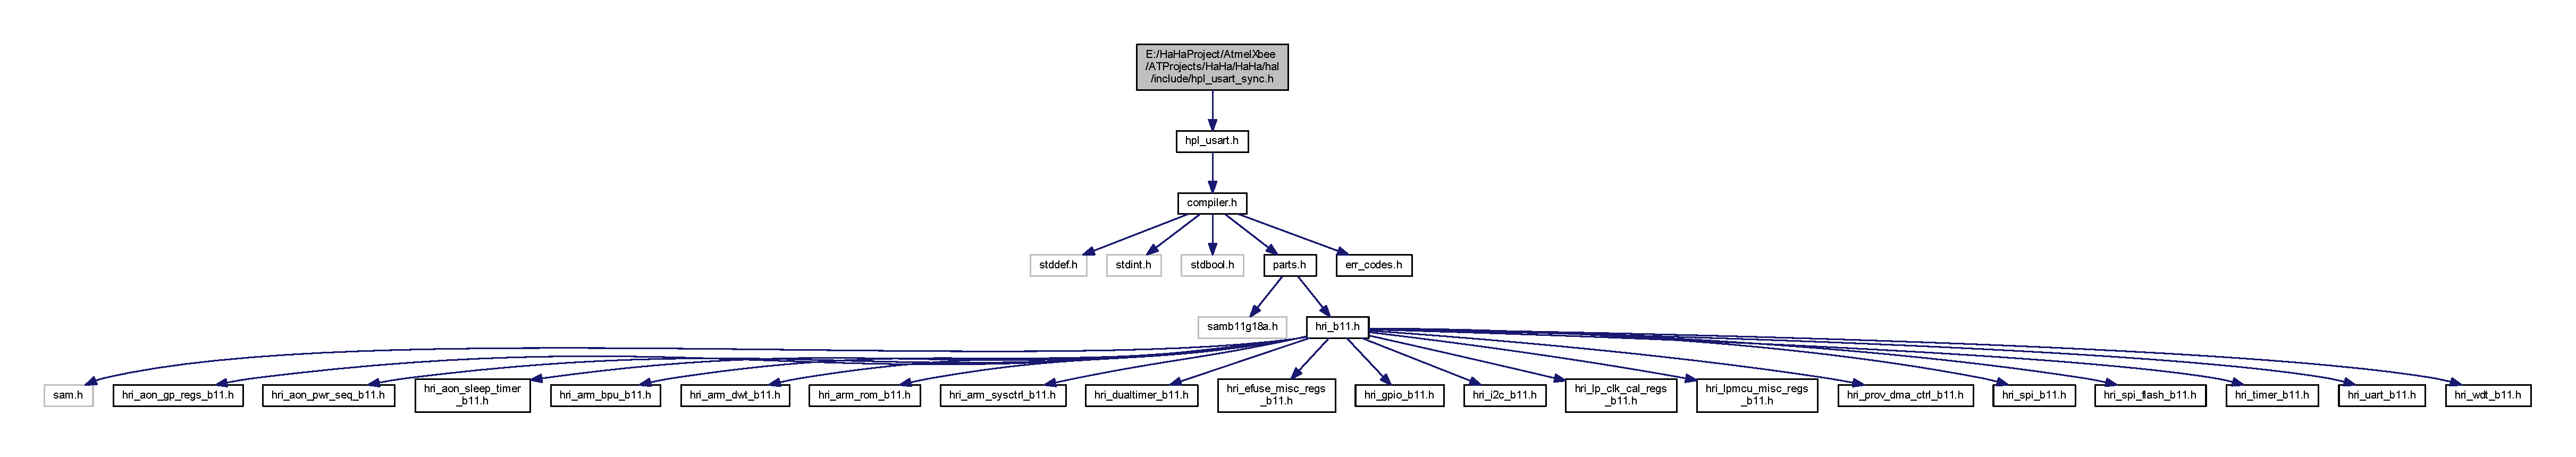
\includegraphics[width=350pt]{hpl__usart__sync_8h__incl}
\end{center}
\end{figure}
This graph shows which files directly or indirectly include this file\+:
\nopagebreak
\begin{figure}[H]
\begin{center}
\leavevmode
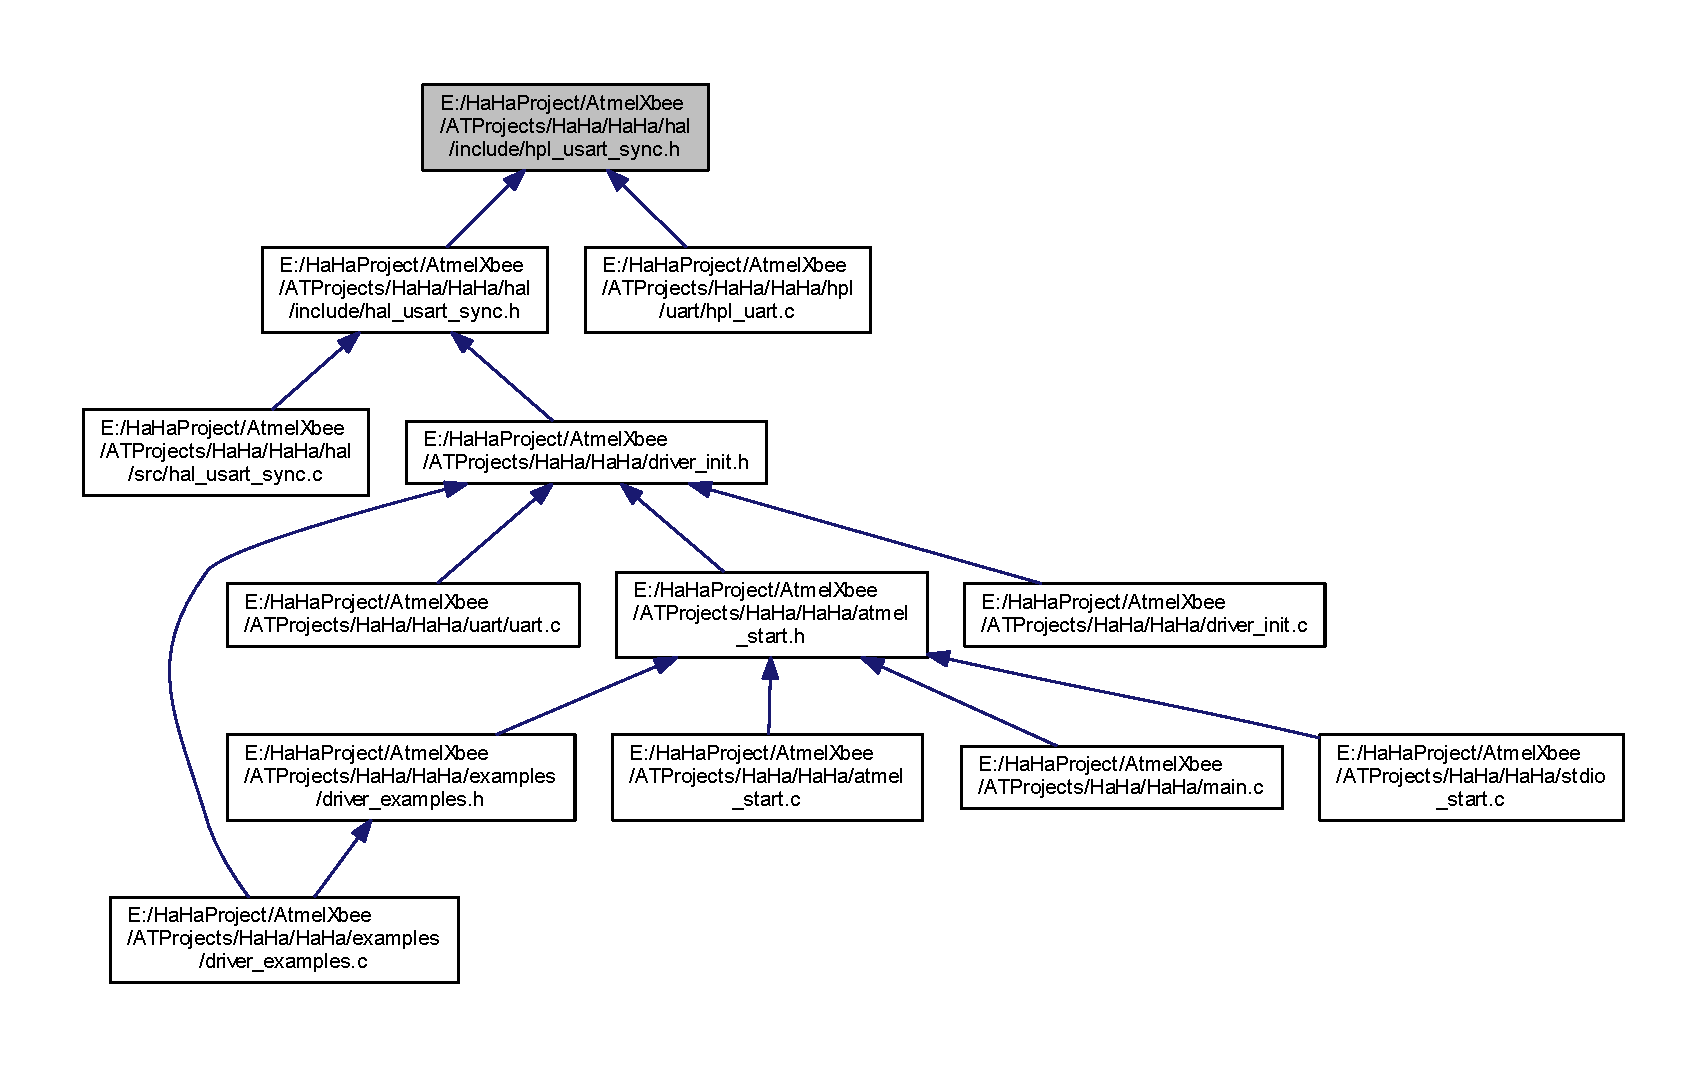
\includegraphics[width=350pt]{hpl__usart__sync_8h__dep__incl}
\end{center}
\end{figure}
\subsection*{Classes}
\begin{DoxyCompactItemize}
\item 
struct \hyperlink{struct__usart__sync__device}{\+\_\+usart\+\_\+sync\+\_\+device}
\begin{DoxyCompactList}\small\item\em U\+S\+A\+RT descriptor device structure. \end{DoxyCompactList}\end{DoxyCompactItemize}
\subsection*{Functions}
\begin{Indent}\textbf{ H\+PL functions}\par
\begin{DoxyCompactItemize}
\item 
int32\+\_\+t \hyperlink{group___h_p_l_gad1cc7b8e72fd67fdeec8062c802eb25a}{\+\_\+usart\+\_\+sync\+\_\+init} (struct \hyperlink{struct__usart__sync__device}{\+\_\+usart\+\_\+sync\+\_\+device} $\ast$const device, void $\ast$const hw)
\begin{DoxyCompactList}\small\item\em Initialize synchronous U\+S\+A\+RT. \end{DoxyCompactList}\item 
void \hyperlink{group___h_p_l_gac046761a56aaedeba5acad135cab707c}{\+\_\+usart\+\_\+sync\+\_\+deinit} (struct \hyperlink{struct__usart__sync__device}{\+\_\+usart\+\_\+sync\+\_\+device} $\ast$const device)
\begin{DoxyCompactList}\small\item\em De-\/initialize U\+S\+A\+RT. \end{DoxyCompactList}\item 
void \hyperlink{group___h_p_l_ga5ca07057bde212b46f6547e5bdb876de}{\+\_\+usart\+\_\+sync\+\_\+enable} (struct \hyperlink{struct__usart__sync__device}{\+\_\+usart\+\_\+sync\+\_\+device} $\ast$const device)
\begin{DoxyCompactList}\small\item\em Enable usart module. \end{DoxyCompactList}\item 
void \hyperlink{group___h_p_l_gac021f29c77d8a9bfabfdd7433dbbb024}{\+\_\+usart\+\_\+sync\+\_\+disable} (struct \hyperlink{struct__usart__sync__device}{\+\_\+usart\+\_\+sync\+\_\+device} $\ast$const device)
\begin{DoxyCompactList}\small\item\em Disable usart module. \end{DoxyCompactList}\item 
uint16\+\_\+t \hyperlink{group___h_p_l_ga0f2e4f3338270295eea1d4e1b00bfa1e}{\+\_\+usart\+\_\+sync\+\_\+calculate\+\_\+baud\+\_\+rate} (const uint32\+\_\+t baud, const uint32\+\_\+t clock\+\_\+rate, const uint8\+\_\+t samples, const enum \hyperlink{group___h_p_l_ga59141b5eb86f4d53f17bbeab1d7c83e7}{usart\+\_\+baud\+\_\+rate\+\_\+mode} mode, const uint8\+\_\+t fraction)
\begin{DoxyCompactList}\small\item\em Calculate baud rate register value. \end{DoxyCompactList}\item 
void \hyperlink{group___h_p_l_ga882c8cecf50eb1276401d6874956b903}{\+\_\+usart\+\_\+sync\+\_\+set\+\_\+baud\+\_\+rate} (struct \hyperlink{struct__usart__sync__device}{\+\_\+usart\+\_\+sync\+\_\+device} $\ast$const device, const uint32\+\_\+t baud\+\_\+rate)
\begin{DoxyCompactList}\small\item\em Set baud rate. \end{DoxyCompactList}\item 
void \hyperlink{group___h_p_l_ga1b30e54d42d94ab59067e121d286d47a}{\+\_\+usart\+\_\+sync\+\_\+set\+\_\+data\+\_\+order} (struct \hyperlink{struct__usart__sync__device}{\+\_\+usart\+\_\+sync\+\_\+device} $\ast$const device, const enum \hyperlink{group___h_p_l_ga426849bbd9655cec091101ebc9123eb4}{usart\+\_\+data\+\_\+order} order)
\begin{DoxyCompactList}\small\item\em Set data order. \end{DoxyCompactList}\item 
void \hyperlink{group___h_p_l_ga2dd82ebe0069e4c61fda94ac0dda1a63}{\+\_\+usart\+\_\+sync\+\_\+set\+\_\+mode} (struct \hyperlink{struct__usart__sync__device}{\+\_\+usart\+\_\+sync\+\_\+device} $\ast$const device, const enum \hyperlink{group___h_p_l_ga1c465965478e0f6908a4c99d4f3ad20f}{usart\+\_\+mode} mode)
\begin{DoxyCompactList}\small\item\em Set mode. \end{DoxyCompactList}\item 
void \hyperlink{group___h_p_l_gaee0a2babdf7b777fa4754028c92fc2e8}{\+\_\+usart\+\_\+sync\+\_\+set\+\_\+parity} (struct \hyperlink{struct__usart__sync__device}{\+\_\+usart\+\_\+sync\+\_\+device} $\ast$const device, const enum \hyperlink{group___h_p_l_ga867cc5f0ea7d3bf651d68f0046cf6f41}{usart\+\_\+parity} parity)
\begin{DoxyCompactList}\small\item\em Set parity. \end{DoxyCompactList}\item 
void \hyperlink{group___h_p_l_ga93c7de4ab355c189e306288d21642ff3}{\+\_\+usart\+\_\+sync\+\_\+set\+\_\+stop\+\_\+bits} (struct \hyperlink{struct__usart__sync__device}{\+\_\+usart\+\_\+sync\+\_\+device} $\ast$const device, const enum \hyperlink{group___h_p_l_ga88311517c5168c29a681604a8a33b06e}{usart\+\_\+stop\+\_\+bits} stop\+\_\+bits)
\begin{DoxyCompactList}\small\item\em Set stop bits mode. \end{DoxyCompactList}\item 
void \hyperlink{group___h_p_l_ga45ebffe94571d266e42b3dd882ad559d}{\+\_\+usart\+\_\+sync\+\_\+set\+\_\+character\+\_\+size} (struct \hyperlink{struct__usart__sync__device}{\+\_\+usart\+\_\+sync\+\_\+device} $\ast$const device, const enum \hyperlink{group___h_p_l_ga631ce7b4f60dccd392e6d6ef7d3cd4e2}{usart\+\_\+character\+\_\+size} size)
\begin{DoxyCompactList}\small\item\em Set character size. \end{DoxyCompactList}\item 
uint32\+\_\+t \hyperlink{group___h_p_l_ga512c769b924d59433542bf347980334b}{\+\_\+usart\+\_\+sync\+\_\+get\+\_\+status} (const struct \hyperlink{struct__usart__sync__device}{\+\_\+usart\+\_\+sync\+\_\+device} $\ast$const device)
\begin{DoxyCompactList}\small\item\em Retrieve usart status. \end{DoxyCompactList}\item 
void \hyperlink{group___h_p_l_ga6f9cc0e2020d49845bef97301bc692e0}{\+\_\+usart\+\_\+sync\+\_\+write\+\_\+byte} (struct \hyperlink{struct__usart__sync__device}{\+\_\+usart\+\_\+sync\+\_\+device} $\ast$const device, uint8\+\_\+t data)
\begin{DoxyCompactList}\small\item\em Write a byte to the given U\+S\+A\+RT instance. \end{DoxyCompactList}\item 
uint8\+\_\+t \hyperlink{group___h_p_l_gad6e42aaa92499103016d605362e35d97}{\+\_\+usart\+\_\+sync\+\_\+read\+\_\+byte} (const struct \hyperlink{struct__usart__sync__device}{\+\_\+usart\+\_\+sync\+\_\+device} $\ast$const device)
\begin{DoxyCompactList}\small\item\em Read a byte from the given U\+S\+A\+RT instance. \end{DoxyCompactList}\item 
bool \hyperlink{group___h_p_l_ga8bad9999c03b728f47848b2337393ec4}{\+\_\+usart\+\_\+sync\+\_\+is\+\_\+byte\+\_\+sent} (const struct \hyperlink{struct__usart__sync__device}{\+\_\+usart\+\_\+sync\+\_\+device} $\ast$const device)
\begin{DoxyCompactList}\small\item\em Check if U\+S\+A\+RT is ready to send next byte. \end{DoxyCompactList}\item 
bool \hyperlink{group___h_p_l_ga5bf04a89be94430de57acf53f9b35dd2}{\+\_\+usart\+\_\+sync\+\_\+is\+\_\+byte\+\_\+received} (const struct \hyperlink{struct__usart__sync__device}{\+\_\+usart\+\_\+sync\+\_\+device} $\ast$const device)
\begin{DoxyCompactList}\small\item\em Check if there is data received by U\+S\+A\+RT. \end{DoxyCompactList}\item 
void \hyperlink{group___h_p_l_gae43bb6755eb8c462a9884e6cdca602aa}{\+\_\+usart\+\_\+sync\+\_\+set\+\_\+flow\+\_\+control\+\_\+state} (struct \hyperlink{struct__usart__sync__device}{\+\_\+usart\+\_\+sync\+\_\+device} $\ast$const device, const union \hyperlink{unionusart__flow__control__state}{usart\+\_\+flow\+\_\+control\+\_\+state} state)
\begin{DoxyCompactList}\small\item\em Set the state of flow control pins. \end{DoxyCompactList}\item 
union \hyperlink{unionusart__flow__control__state}{usart\+\_\+flow\+\_\+control\+\_\+state} \hyperlink{group___h_p_l_ga5b6662f283d7a2791c7eed77635e9238}{\+\_\+usart\+\_\+sync\+\_\+get\+\_\+flow\+\_\+control\+\_\+state} (const struct \hyperlink{struct__usart__sync__device}{\+\_\+usart\+\_\+sync\+\_\+device} $\ast$const device)
\begin{DoxyCompactList}\small\item\em Retrieve the state of flow control pins. \end{DoxyCompactList}\item 
uint8\+\_\+t \hyperlink{group___h_p_l_ga8fd6539ded0699161df00f23ba6580aa}{\+\_\+usart\+\_\+sync\+\_\+get\+\_\+hardware\+\_\+index} (const struct \hyperlink{struct__usart__sync__device}{\+\_\+usart\+\_\+sync\+\_\+device} $\ast$const device)
\begin{DoxyCompactList}\small\item\em Retrieve ordinal number of the given U\+S\+A\+RT hardware instance. \end{DoxyCompactList}\end{DoxyCompactItemize}
\end{Indent}


\subsection{Detailed Description}
U\+S\+A\+RT related functionality declaration. 

Copyright (C) 2014 Atmel Corporation. All rights reserved.
\hypertarget{hal__atomic_8c}{}\section{E\+:/\+Ha\+Ha\+Project/\+Atmel\+Xbee/\+A\+T\+Projects/\+Ha\+Ha/\+Ha\+Ha/hal/src/hal\+\_\+atomic.c File Reference}
\label{hal__atomic_8c}\index{E\+:/\+Ha\+Ha\+Project/\+Atmel\+Xbee/\+A\+T\+Projects/\+Ha\+Ha/\+Ha\+Ha/hal/src/hal\+\_\+atomic.\+c@{E\+:/\+Ha\+Ha\+Project/\+Atmel\+Xbee/\+A\+T\+Projects/\+Ha\+Ha/\+Ha\+Ha/hal/src/hal\+\_\+atomic.\+c}}


Critical sections related functionality implementation.  


{\ttfamily \#include \char`\"{}hal\+\_\+atomic.\+h\char`\"{}}\newline
\subsection*{Macros}
\begin{DoxyCompactItemize}
\item 
\mbox{\Hypertarget{hal__atomic_8c_ae578001fe043b4cca7a0edd801cfe9c4}\label{hal__atomic_8c_ae578001fe043b4cca7a0edd801cfe9c4}} 
\#define \hyperlink{hal__atomic_8c_ae578001fe043b4cca7a0edd801cfe9c4}{D\+R\+I\+V\+E\+R\+\_\+\+V\+E\+R\+S\+I\+ON}~0x00000001u
\begin{DoxyCompactList}\small\item\em Driver version. \end{DoxyCompactList}\end{DoxyCompactItemize}
\subsection*{Functions}
\begin{DoxyCompactItemize}
\item 
void \hyperlink{group__doc__driver__hal__helper__atomic_ga3bd20e6e0bdec53177758490510ba916}{atomic\+\_\+enter\+\_\+critical} (\hyperlink{group__doc__driver__hal__helper__atomic_ga6b3a0c9eea25111ac1877e0302e2fe1c}{hal\+\_\+atomic\+\_\+t} volatile $\ast$atomic)
\begin{DoxyCompactList}\small\item\em Disable interrupts, enter critical section. \end{DoxyCompactList}\item 
void \hyperlink{group__doc__driver__hal__helper__atomic_gaef0ccaa2438aca5ea074b36252d65990}{atomic\+\_\+leave\+\_\+critical} (\hyperlink{group__doc__driver__hal__helper__atomic_ga6b3a0c9eea25111ac1877e0302e2fe1c}{hal\+\_\+atomic\+\_\+t} volatile $\ast$atomic)
\begin{DoxyCompactList}\small\item\em Exit atomic section. \end{DoxyCompactList}\item 
uint32\+\_\+t \hyperlink{group__doc__driver__hal__helper__atomic_ga75fe13100e2799eb24a80123bc8c3787}{atomic\+\_\+get\+\_\+version} (void)
\begin{DoxyCompactList}\small\item\em Retrieve the current driver version. \end{DoxyCompactList}\end{DoxyCompactItemize}


\subsection{Detailed Description}
Critical sections related functionality implementation. 

Copyright (C) 2014 Atmel Corporation. All rights reserved.
\hypertarget{hal__gpio_8c}{}\section{E\+:/\+Ha\+Ha\+Project/\+Atmel\+Xbee/\+A\+T\+Projects/\+Ha\+Ha/\+Ha\+Ha/hal/src/hal\+\_\+gpio.c File Reference}
\label{hal__gpio_8c}\index{E\+:/\+Ha\+Ha\+Project/\+Atmel\+Xbee/\+A\+T\+Projects/\+Ha\+Ha/\+Ha\+Ha/hal/src/hal\+\_\+gpio.\+c@{E\+:/\+Ha\+Ha\+Project/\+Atmel\+Xbee/\+A\+T\+Projects/\+Ha\+Ha/\+Ha\+Ha/hal/src/hal\+\_\+gpio.\+c}}


Port.  


{\ttfamily \#include \char`\"{}hal\+\_\+gpio.\+h\char`\"{}}\newline
\subsection*{Macros}
\begin{DoxyCompactItemize}
\item 
\mbox{\Hypertarget{hal__gpio_8c_ae578001fe043b4cca7a0edd801cfe9c4}\label{hal__gpio_8c_ae578001fe043b4cca7a0edd801cfe9c4}} 
\#define \hyperlink{hal__gpio_8c_ae578001fe043b4cca7a0edd801cfe9c4}{D\+R\+I\+V\+E\+R\+\_\+\+V\+E\+R\+S\+I\+ON}~0x00000001u
\begin{DoxyCompactList}\small\item\em Driver version. \end{DoxyCompactList}\end{DoxyCompactItemize}
\subsection*{Functions}
\begin{DoxyCompactItemize}
\item 
\mbox{\Hypertarget{hal__gpio_8c_a19c3104daa7a427258fc4d1ba26db13b}\label{hal__gpio_8c_a19c3104daa7a427258fc4d1ba26db13b}} 
uint32\+\_\+t \hyperlink{hal__gpio_8c_a19c3104daa7a427258fc4d1ba26db13b}{gpio\+\_\+get\+\_\+version} (void)
\begin{DoxyCompactList}\small\item\em Get current driver version. \end{DoxyCompactList}\end{DoxyCompactItemize}


\subsection{Detailed Description}
Port. 

Copyright (C) 2014 Atmel Corporation. All rights reserved.
\hypertarget{hal__init_8c}{}\section{E\+:/\+Ha\+Ha\+Project/\+Atmel\+Xbee/\+A\+T\+Projects/\+Ha\+Ha/\+Ha\+Ha/hal/src/hal\+\_\+init.c File Reference}
\label{hal__init_8c}\index{E\+:/\+Ha\+Ha\+Project/\+Atmel\+Xbee/\+A\+T\+Projects/\+Ha\+Ha/\+Ha\+Ha/hal/src/hal\+\_\+init.\+c@{E\+:/\+Ha\+Ha\+Project/\+Atmel\+Xbee/\+A\+T\+Projects/\+Ha\+Ha/\+Ha\+Ha/hal/src/hal\+\_\+init.\+c}}


H\+AL initialization related functionality implementation.  


{\ttfamily \#include \char`\"{}hal\+\_\+init.\+h\char`\"{}}\newline
Include dependency graph for hal\+\_\+init.\+c\+:
\nopagebreak
\begin{figure}[H]
\begin{center}
\leavevmode
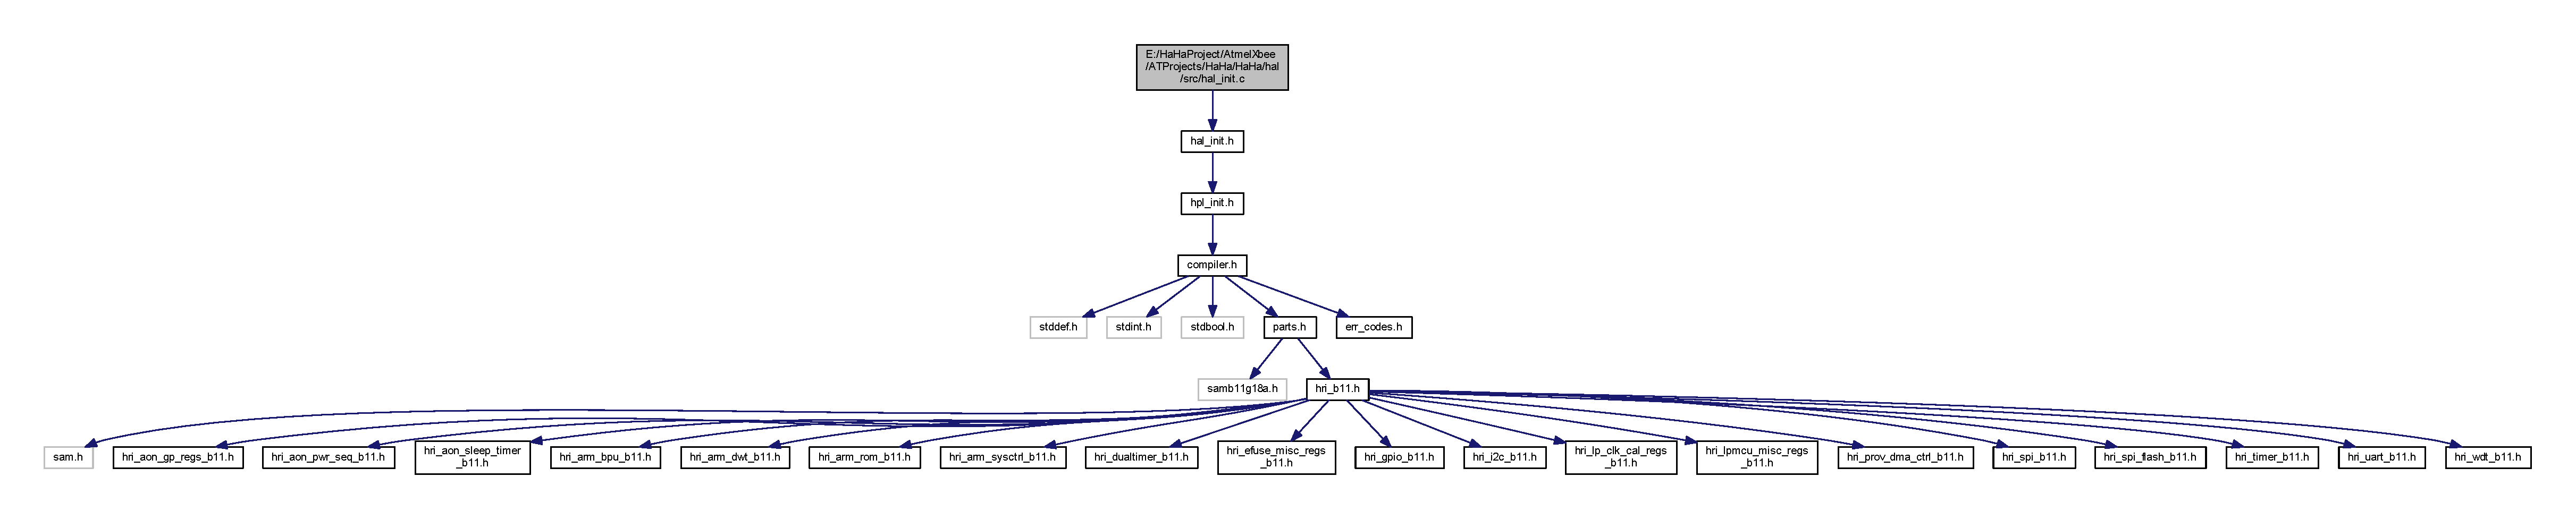
\includegraphics[width=350pt]{hal__init_8c__incl}
\end{center}
\end{figure}
\subsection*{Macros}
\begin{DoxyCompactItemize}
\item 
\#define \hyperlink{hal__init_8c_a3301dd997160623636cbfc73ca164ef5}{H\+A\+L\+\_\+\+I\+N\+I\+T\+\_\+\+V\+E\+R\+S\+I\+ON}~0x00000001u
\begin{DoxyCompactList}\small\item\em Driver version. \end{DoxyCompactList}\end{DoxyCompactItemize}
\subsection*{Functions}
\begin{DoxyCompactItemize}
\item 
uint32\+\_\+t \hyperlink{group__doc__driver__hal__helper__init_ga7f3a0a79c14d4043ea30435f561af05f}{init\+\_\+get\+\_\+version} (void)
\begin{DoxyCompactList}\small\item\em Retrieve the current driver version. \end{DoxyCompactList}\end{DoxyCompactItemize}


\subsection{Detailed Description}
H\+AL initialization related functionality implementation. 

Copyright (C) 2014-\/2015 Atmel Corporation. All rights reserved.

\subsection{Macro Definition Documentation}
\mbox{\Hypertarget{hal__init_8c_a3301dd997160623636cbfc73ca164ef5}\label{hal__init_8c_a3301dd997160623636cbfc73ca164ef5}} 
\index{hal\+\_\+init.\+c@{hal\+\_\+init.\+c}!H\+A\+L\+\_\+\+I\+N\+I\+T\+\_\+\+V\+E\+R\+S\+I\+ON@{H\+A\+L\+\_\+\+I\+N\+I\+T\+\_\+\+V\+E\+R\+S\+I\+ON}}
\index{H\+A\+L\+\_\+\+I\+N\+I\+T\+\_\+\+V\+E\+R\+S\+I\+ON@{H\+A\+L\+\_\+\+I\+N\+I\+T\+\_\+\+V\+E\+R\+S\+I\+ON}!hal\+\_\+init.\+c@{hal\+\_\+init.\+c}}
\subsubsection{\texorpdfstring{H\+A\+L\+\_\+\+I\+N\+I\+T\+\_\+\+V\+E\+R\+S\+I\+ON}{HAL\_INIT\_VERSION}}
{\footnotesize\ttfamily \#define H\+A\+L\+\_\+\+I\+N\+I\+T\+\_\+\+V\+E\+R\+S\+I\+ON~0x00000001u}



Driver version. 


\hypertarget{hal__io_8c}{}\section{E\+:/\+Ha\+Ha\+Project/\+Atmel\+Xbee/\+A\+T\+Projects/\+Ha\+Ha/\+Ha\+Ha/hal/src/hal\+\_\+io.c File Reference}
\label{hal__io_8c}\index{E\+:/\+Ha\+Ha\+Project/\+Atmel\+Xbee/\+A\+T\+Projects/\+Ha\+Ha/\+Ha\+Ha/hal/src/hal\+\_\+io.\+c@{E\+:/\+Ha\+Ha\+Project/\+Atmel\+Xbee/\+A\+T\+Projects/\+Ha\+Ha/\+Ha\+Ha/hal/src/hal\+\_\+io.\+c}}


IO functionality implementation.  


{\ttfamily \#include $<$hal\+\_\+io.\+h$>$}\newline
{\ttfamily \#include $<$utils\+\_\+assert.\+h$>$}\newline
Include dependency graph for hal\+\_\+io.\+c\+:
\nopagebreak
\begin{figure}[H]
\begin{center}
\leavevmode
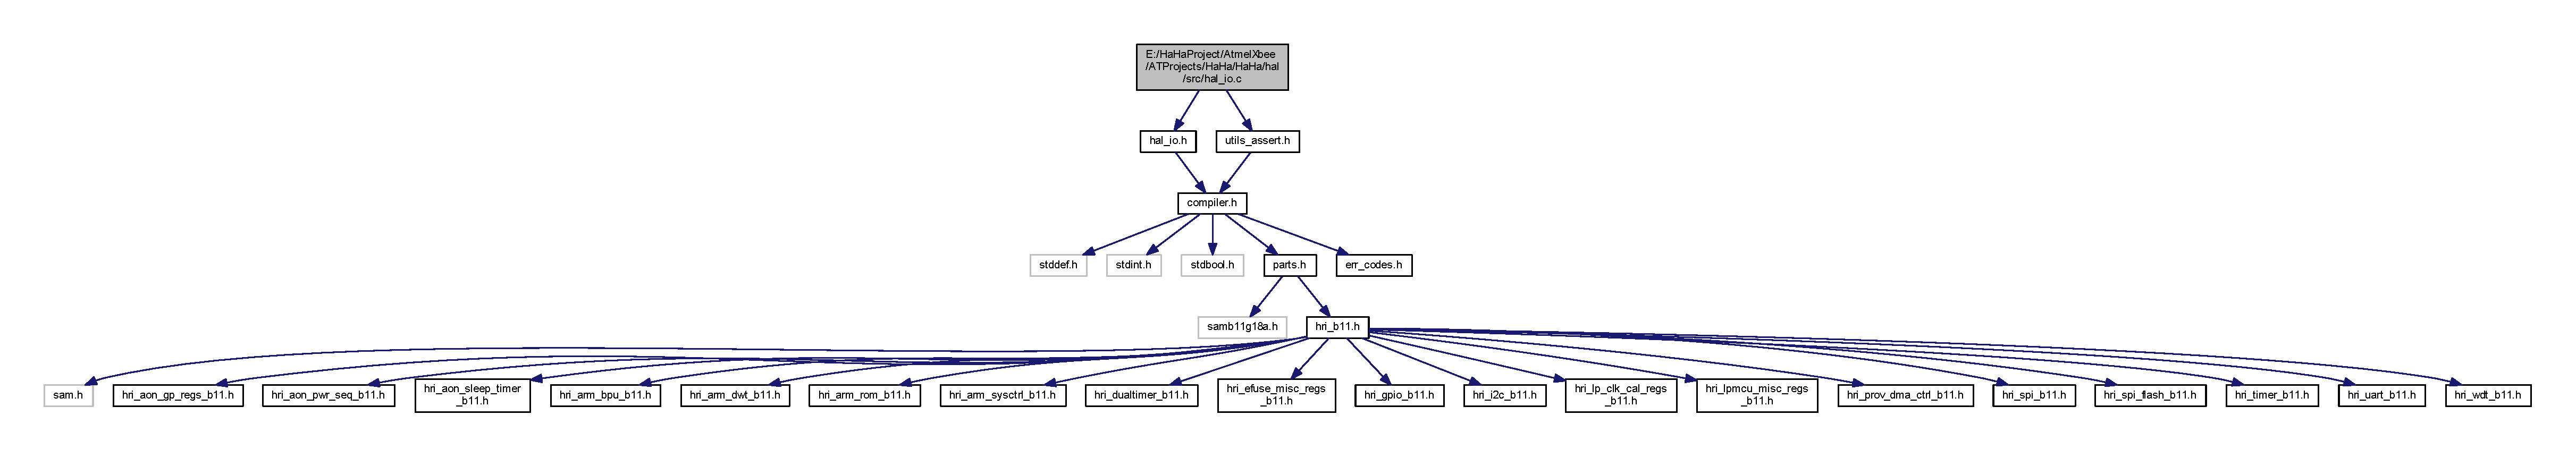
\includegraphics[width=350pt]{hal__io_8c__incl}
\end{center}
\end{figure}
\subsection*{Macros}
\begin{DoxyCompactItemize}
\item 
\#define \hyperlink{hal__io_8c_ae578001fe043b4cca7a0edd801cfe9c4}{D\+R\+I\+V\+E\+R\+\_\+\+V\+E\+R\+S\+I\+ON}~0x00000001u
\begin{DoxyCompactList}\small\item\em Driver version. \end{DoxyCompactList}\end{DoxyCompactItemize}
\subsection*{Functions}
\begin{DoxyCompactItemize}
\item 
uint32\+\_\+t \hyperlink{hal__io_8c_a081053bb07051453fcafb199d9ff4504}{io\+\_\+get\+\_\+version} (void)
\item 
int32\+\_\+t \hyperlink{group__doc__driver__hal__helper__io_ga81aac60d5ce6feb0c44f8937d7c02f14}{io\+\_\+write} (struct \hyperlink{structio__descriptor}{io\+\_\+descriptor} $\ast$const io\+\_\+descr, const uint8\+\_\+t $\ast$const buf, const uint16\+\_\+t length)
\begin{DoxyCompactList}\small\item\em IO write interface. \end{DoxyCompactList}\item 
int32\+\_\+t \hyperlink{group__doc__driver__hal__helper__io_gaf5e8722129933fa8e014144fd7505be6}{io\+\_\+read} (struct \hyperlink{structio__descriptor}{io\+\_\+descriptor} $\ast$const io\+\_\+descr, uint8\+\_\+t $\ast$const buf, const uint16\+\_\+t length)
\begin{DoxyCompactList}\small\item\em IO read interface. \end{DoxyCompactList}\end{DoxyCompactItemize}


\subsection{Detailed Description}
IO functionality implementation. 

Copyright (C) 2015 Atmel Corporation. All rights reserved.

\subsection{Macro Definition Documentation}
\mbox{\Hypertarget{hal__io_8c_ae578001fe043b4cca7a0edd801cfe9c4}\label{hal__io_8c_ae578001fe043b4cca7a0edd801cfe9c4}} 
\index{hal\+\_\+io.\+c@{hal\+\_\+io.\+c}!D\+R\+I\+V\+E\+R\+\_\+\+V\+E\+R\+S\+I\+ON@{D\+R\+I\+V\+E\+R\+\_\+\+V\+E\+R\+S\+I\+ON}}
\index{D\+R\+I\+V\+E\+R\+\_\+\+V\+E\+R\+S\+I\+ON@{D\+R\+I\+V\+E\+R\+\_\+\+V\+E\+R\+S\+I\+ON}!hal\+\_\+io.\+c@{hal\+\_\+io.\+c}}
\subsubsection{\texorpdfstring{D\+R\+I\+V\+E\+R\+\_\+\+V\+E\+R\+S\+I\+ON}{DRIVER\_VERSION}}
{\footnotesize\ttfamily \#define D\+R\+I\+V\+E\+R\+\_\+\+V\+E\+R\+S\+I\+ON~0x00000001u}



Driver version. 



\subsection{Function Documentation}
\mbox{\Hypertarget{hal__io_8c_a081053bb07051453fcafb199d9ff4504}\label{hal__io_8c_a081053bb07051453fcafb199d9ff4504}} 
\index{hal\+\_\+io.\+c@{hal\+\_\+io.\+c}!io\+\_\+get\+\_\+version@{io\+\_\+get\+\_\+version}}
\index{io\+\_\+get\+\_\+version@{io\+\_\+get\+\_\+version}!hal\+\_\+io.\+c@{hal\+\_\+io.\+c}}
\subsubsection{\texorpdfstring{io\+\_\+get\+\_\+version()}{io\_get\_version()}}
{\footnotesize\ttfamily uint32\+\_\+t io\+\_\+get\+\_\+version (\begin{DoxyParamCaption}\item[{void}]{ }\end{DoxyParamCaption})}


\hypertarget{hal__usart__async_8c}{}\section{E\+:/\+Ha\+Ha\+Project/\+Atmel\+Xbee/\+A\+T\+Projects/\+Ha\+Ha/\+Ha\+Ha/hal/src/hal\+\_\+usart\+\_\+async.c File Reference}
\label{hal__usart__async_8c}\index{E\+:/\+Ha\+Ha\+Project/\+Atmel\+Xbee/\+A\+T\+Projects/\+Ha\+Ha/\+Ha\+Ha/hal/src/hal\+\_\+usart\+\_\+async.\+c@{E\+:/\+Ha\+Ha\+Project/\+Atmel\+Xbee/\+A\+T\+Projects/\+Ha\+Ha/\+Ha\+Ha/hal/src/hal\+\_\+usart\+\_\+async.\+c}}


IO U\+S\+A\+RT related functionality implementation.  


{\ttfamily \#include \char`\"{}hal\+\_\+usart\+\_\+async.\+h\char`\"{}}\newline
{\ttfamily \#include $<$utils\+\_\+assert.\+h$>$}\newline
{\ttfamily \#include $<$hal\+\_\+atomic.\+h$>$}\newline
{\ttfamily \#include $<$utils.\+h$>$}\newline
\subsection*{Macros}
\begin{DoxyCompactItemize}
\item 
\mbox{\Hypertarget{hal__usart__async_8c_ae578001fe043b4cca7a0edd801cfe9c4}\label{hal__usart__async_8c_ae578001fe043b4cca7a0edd801cfe9c4}} 
\#define \hyperlink{hal__usart__async_8c_ae578001fe043b4cca7a0edd801cfe9c4}{D\+R\+I\+V\+E\+R\+\_\+\+V\+E\+R\+S\+I\+ON}~0x00000001u
\begin{DoxyCompactList}\small\item\em Driver version. \end{DoxyCompactList}\end{DoxyCompactItemize}
\subsection*{Functions}
\begin{DoxyCompactItemize}
\item 
int32\+\_\+t \hyperlink{group__doc__driver__hal__usart__async_gaafe146c618b950c9715efb0fdc6a7484}{usart\+\_\+async\+\_\+init} (struct \hyperlink{structusart__async__descriptor}{usart\+\_\+async\+\_\+descriptor} $\ast$const descr, void $\ast$const hw, uint8\+\_\+t $\ast$rx\+\_\+buffer, uint16\+\_\+t rx\+\_\+buffer\+\_\+length, void $\ast$const func)
\begin{DoxyCompactList}\small\item\em Initialize usart interface. \end{DoxyCompactList}\item 
int32\+\_\+t \hyperlink{group__doc__driver__hal__usart__async_gab7ef65ba7b4afd13cb11dcc72315ca43}{usart\+\_\+async\+\_\+deinit} (struct \hyperlink{structusart__async__descriptor}{usart\+\_\+async\+\_\+descriptor} $\ast$const descr)
\begin{DoxyCompactList}\small\item\em De-\/initialize usart interface. \end{DoxyCompactList}\item 
int32\+\_\+t \hyperlink{group__doc__driver__hal__usart__async_gaa752e7d978b7f3bc35c97f9a7eb5f98a}{usart\+\_\+async\+\_\+enable} (struct \hyperlink{structusart__async__descriptor}{usart\+\_\+async\+\_\+descriptor} $\ast$const descr)
\begin{DoxyCompactList}\small\item\em Enable usart interface. \end{DoxyCompactList}\item 
int32\+\_\+t \hyperlink{group__doc__driver__hal__usart__async_ga575b7b546a7357088530a9cebf60ad9a}{usart\+\_\+async\+\_\+disable} (struct \hyperlink{structusart__async__descriptor}{usart\+\_\+async\+\_\+descriptor} $\ast$const descr)
\begin{DoxyCompactList}\small\item\em Disable usart interface. \end{DoxyCompactList}\item 
int32\+\_\+t \hyperlink{group__doc__driver__hal__usart__async_ga964be25acbad24e7d0cb9e72f5f5582f}{usart\+\_\+async\+\_\+get\+\_\+io\+\_\+descriptor} (struct \hyperlink{structusart__async__descriptor}{usart\+\_\+async\+\_\+descriptor} $\ast$const descr, struct \hyperlink{structio__descriptor}{io\+\_\+descriptor} $\ast$$\ast$io)
\begin{DoxyCompactList}\small\item\em Retrieve IO descriptor. \end{DoxyCompactList}\item 
int32\+\_\+t \hyperlink{group__doc__driver__hal__usart__async_ga2d7d4ba3ab10f19c2e8a7901f2b6b276}{usart\+\_\+async\+\_\+register\+\_\+callback} (struct \hyperlink{structusart__async__descriptor}{usart\+\_\+async\+\_\+descriptor} $\ast$const descr, const enum \hyperlink{group__doc__driver__hal__usart__async_ga5a82ef383f62daa061a55838c8fc6d39}{usart\+\_\+async\+\_\+callback\+\_\+type} type, \hyperlink{group__doc__driver__hal__usart__async_ga430e4080a53e1f39c4d46da01200f633}{usart\+\_\+cb\+\_\+t} cb)
\begin{DoxyCompactList}\small\item\em Register usart callback. \end{DoxyCompactList}\item 
int32\+\_\+t \hyperlink{group__doc__driver__hal__usart__async_gacbc3f9aec99169e42d49555cf829a3d1}{usart\+\_\+async\+\_\+set\+\_\+flow\+\_\+control} (struct \hyperlink{structusart__async__descriptor}{usart\+\_\+async\+\_\+descriptor} $\ast$const descr, const union \hyperlink{unionusart__flow__control__state}{usart\+\_\+flow\+\_\+control\+\_\+state} state)
\begin{DoxyCompactList}\small\item\em Specify action for flow control pins. \end{DoxyCompactList}\item 
int32\+\_\+t \hyperlink{group__doc__driver__hal__usart__async_gab6bb473a5047ae890b1406ffcca3042d}{usart\+\_\+async\+\_\+set\+\_\+baud\+\_\+rate} (struct \hyperlink{structusart__async__descriptor}{usart\+\_\+async\+\_\+descriptor} $\ast$const descr, const uint32\+\_\+t baud\+\_\+rate)
\begin{DoxyCompactList}\small\item\em Set usart baud rate. \end{DoxyCompactList}\item 
int32\+\_\+t \hyperlink{group__doc__driver__hal__usart__async_ga1ed416c72b54e87f8da098f148e0c7fc}{usart\+\_\+async\+\_\+set\+\_\+data\+\_\+order} (struct \hyperlink{structusart__async__descriptor}{usart\+\_\+async\+\_\+descriptor} $\ast$const descr, const enum \hyperlink{group___h_p_l_ga426849bbd9655cec091101ebc9123eb4}{usart\+\_\+data\+\_\+order} data\+\_\+order)
\begin{DoxyCompactList}\small\item\em Set usart data order. \end{DoxyCompactList}\item 
int32\+\_\+t \hyperlink{group__doc__driver__hal__usart__async_ga8b2ee777456a88b7843366761a8356c9}{usart\+\_\+async\+\_\+set\+\_\+mode} (struct \hyperlink{structusart__async__descriptor}{usart\+\_\+async\+\_\+descriptor} $\ast$const descr, const enum \hyperlink{group___h_p_l_ga1c465965478e0f6908a4c99d4f3ad20f}{usart\+\_\+mode} mode)
\begin{DoxyCompactList}\small\item\em Set usart mode. \end{DoxyCompactList}\item 
int32\+\_\+t \hyperlink{group__doc__driver__hal__usart__async_ga6cee441159bf41f74a105042fb6c8477}{usart\+\_\+async\+\_\+set\+\_\+parity} (struct \hyperlink{structusart__async__descriptor}{usart\+\_\+async\+\_\+descriptor} $\ast$const descr, const enum \hyperlink{group___h_p_l_ga867cc5f0ea7d3bf651d68f0046cf6f41}{usart\+\_\+parity} parity)
\begin{DoxyCompactList}\small\item\em Set usart parity. \end{DoxyCompactList}\item 
int32\+\_\+t \hyperlink{group__doc__driver__hal__usart__async_ga1749b4fd6293a49428cf4baf74656dd5}{usart\+\_\+async\+\_\+set\+\_\+stopbits} (struct \hyperlink{structusart__async__descriptor}{usart\+\_\+async\+\_\+descriptor} $\ast$const descr, const enum \hyperlink{group___h_p_l_ga88311517c5168c29a681604a8a33b06e}{usart\+\_\+stop\+\_\+bits} stop\+\_\+bits)
\begin{DoxyCompactList}\small\item\em Set usart stop bits. \end{DoxyCompactList}\item 
int32\+\_\+t \hyperlink{group__doc__driver__hal__usart__async_ga949ebae93032ed1a276be009cc1539d6}{usart\+\_\+async\+\_\+set\+\_\+character\+\_\+size} (struct \hyperlink{structusart__async__descriptor}{usart\+\_\+async\+\_\+descriptor} $\ast$const descr, const enum \hyperlink{group___h_p_l_ga631ce7b4f60dccd392e6d6ef7d3cd4e2}{usart\+\_\+character\+\_\+size} size)
\begin{DoxyCompactList}\small\item\em Set usart character size. \end{DoxyCompactList}\item 
int32\+\_\+t \hyperlink{group__doc__driver__hal__usart__async_gaf451cb5a13be66b9357354b1b503c892}{usart\+\_\+async\+\_\+flow\+\_\+control\+\_\+status} (const struct \hyperlink{structusart__async__descriptor}{usart\+\_\+async\+\_\+descriptor} $\ast$const descr, union \hyperlink{unionusart__flow__control__state}{usart\+\_\+flow\+\_\+control\+\_\+state} $\ast$const state)
\begin{DoxyCompactList}\small\item\em Retrieve the state of flow control pins. \end{DoxyCompactList}\item 
int32\+\_\+t \hyperlink{group__doc__driver__hal__usart__async_ga25db066e0587014aab7038cc9295b177}{usart\+\_\+async\+\_\+is\+\_\+tx\+\_\+empty} (const struct \hyperlink{structusart__async__descriptor}{usart\+\_\+async\+\_\+descriptor} $\ast$const descr)
\begin{DoxyCompactList}\small\item\em Check if the usart transmitter is empty. \end{DoxyCompactList}\item 
int32\+\_\+t \hyperlink{group__doc__driver__hal__usart__async_gac8f1c592dc9a82c918eb5c7b2d036963}{usart\+\_\+async\+\_\+is\+\_\+rx\+\_\+not\+\_\+empty} (const struct \hyperlink{structusart__async__descriptor}{usart\+\_\+async\+\_\+descriptor} $\ast$const descr)
\begin{DoxyCompactList}\small\item\em Check if the usart receiver is not empty. \end{DoxyCompactList}\item 
int32\+\_\+t \hyperlink{group__doc__driver__hal__usart__async_gabf0f8fdd20b3b586cb5c0d7fcd4e2114}{usart\+\_\+async\+\_\+get\+\_\+status} (struct \hyperlink{structusart__async__descriptor}{usart\+\_\+async\+\_\+descriptor} $\ast$const descr, struct \hyperlink{structusart__async__status}{usart\+\_\+async\+\_\+status} $\ast$const status)
\begin{DoxyCompactList}\small\item\em Retrieve the current interface status. \end{DoxyCompactList}\item 
int32\+\_\+t \hyperlink{group__doc__driver__hal__usart__async_gaaccb76b1f2ca76451e29b1f674a0c646}{usart\+\_\+async\+\_\+flush\+\_\+rx\+\_\+buffer} (struct \hyperlink{structusart__async__descriptor}{usart\+\_\+async\+\_\+descriptor} $\ast$const descr)
\begin{DoxyCompactList}\small\item\em flush usart rx ringbuf \end{DoxyCompactList}\item 
uint32\+\_\+t \hyperlink{group__doc__driver__hal__usart__async_ga8fd83888546106a6a65e1951e4065d9f}{usart\+\_\+async\+\_\+get\+\_\+version} (void)
\begin{DoxyCompactList}\small\item\em Retrieve the current driver version. \end{DoxyCompactList}\end{DoxyCompactItemize}


\subsection{Detailed Description}
IO U\+S\+A\+RT related functionality implementation. 

Copyright (C) 2014 -\/ 2016 Atmel Corporation. All rights reserved.
\hypertarget{hal__usart__sync_8c}{}\section{E\+:/\+Ha\+Ha\+Project/\+Atmel\+Xbee/\+A\+T\+Projects/\+Ha\+Ha/\+Ha\+Ha/hal/src/hal\+\_\+usart\+\_\+sync.c File Reference}
\label{hal__usart__sync_8c}\index{E\+:/\+Ha\+Ha\+Project/\+Atmel\+Xbee/\+A\+T\+Projects/\+Ha\+Ha/\+Ha\+Ha/hal/src/hal\+\_\+usart\+\_\+sync.\+c@{E\+:/\+Ha\+Ha\+Project/\+Atmel\+Xbee/\+A\+T\+Projects/\+Ha\+Ha/\+Ha\+Ha/hal/src/hal\+\_\+usart\+\_\+sync.\+c}}


IO U\+S\+A\+RT related functionality implementation.  


{\ttfamily \#include \char`\"{}hal\+\_\+usart\+\_\+sync.\+h\char`\"{}}\newline
{\ttfamily \#include $<$utils\+\_\+assert.\+h$>$}\newline
{\ttfamily \#include $<$utils.\+h$>$}\newline
\subsection*{Macros}
\begin{DoxyCompactItemize}
\item 
\mbox{\Hypertarget{hal__usart__sync_8c_ae578001fe043b4cca7a0edd801cfe9c4}\label{hal__usart__sync_8c_ae578001fe043b4cca7a0edd801cfe9c4}} 
\#define \hyperlink{hal__usart__sync_8c_ae578001fe043b4cca7a0edd801cfe9c4}{D\+R\+I\+V\+E\+R\+\_\+\+V\+E\+R\+S\+I\+ON}~0x00000001u
\begin{DoxyCompactList}\small\item\em Driver version. \end{DoxyCompactList}\end{DoxyCompactItemize}
\subsection*{Functions}
\begin{DoxyCompactItemize}
\item 
int32\+\_\+t \hyperlink{group__doc__driver__hal__usart__sync_gaa3cca792d7af7f180c5084af8ffd11c3}{usart\+\_\+sync\+\_\+init} (struct \hyperlink{structusart__sync__descriptor}{usart\+\_\+sync\+\_\+descriptor} $\ast$const descr, void $\ast$const hw, void $\ast$const func)
\begin{DoxyCompactList}\small\item\em Initialize usart interface. \end{DoxyCompactList}\item 
int32\+\_\+t \hyperlink{group__doc__driver__hal__usart__sync_gae8076ed0a30199bd526f1da22e2095d3}{usart\+\_\+sync\+\_\+deinit} (struct \hyperlink{structusart__sync__descriptor}{usart\+\_\+sync\+\_\+descriptor} $\ast$const descr)
\begin{DoxyCompactList}\small\item\em Uninitialize usart interface. \end{DoxyCompactList}\item 
int32\+\_\+t \hyperlink{group__doc__driver__hal__usart__sync_ga351aa9c8c94b4e8b0eb5efb1ecd74a82}{usart\+\_\+sync\+\_\+enable} (struct \hyperlink{structusart__sync__descriptor}{usart\+\_\+sync\+\_\+descriptor} $\ast$const descr)
\begin{DoxyCompactList}\small\item\em Enable usart interface. \end{DoxyCompactList}\item 
int32\+\_\+t \hyperlink{group__doc__driver__hal__usart__sync_ga76abe691b76e4b95b4e3a7d5bc79b026}{usart\+\_\+sync\+\_\+disable} (struct \hyperlink{structusart__sync__descriptor}{usart\+\_\+sync\+\_\+descriptor} $\ast$const descr)
\begin{DoxyCompactList}\small\item\em Disable usart interface. \end{DoxyCompactList}\item 
int32\+\_\+t \hyperlink{group__doc__driver__hal__usart__sync_gaf0b9c8819dc24f75e4f87f050edc81f5}{usart\+\_\+sync\+\_\+get\+\_\+io\+\_\+descriptor} (struct \hyperlink{structusart__sync__descriptor}{usart\+\_\+sync\+\_\+descriptor} $\ast$const descr, struct \hyperlink{structio__descriptor}{io\+\_\+descriptor} $\ast$$\ast$io)
\begin{DoxyCompactList}\small\item\em Retrieve IO descriptor. \end{DoxyCompactList}\item 
int32\+\_\+t \hyperlink{group__doc__driver__hal__usart__sync_ga23977cbdcabc4a624dde31be5ebba482}{usart\+\_\+sync\+\_\+set\+\_\+flow\+\_\+control} (struct \hyperlink{structusart__sync__descriptor}{usart\+\_\+sync\+\_\+descriptor} $\ast$const descr, const union \hyperlink{unionusart__flow__control__state}{usart\+\_\+flow\+\_\+control\+\_\+state} state)
\begin{DoxyCompactList}\small\item\em Specify action for flow control pins. \end{DoxyCompactList}\item 
int32\+\_\+t \hyperlink{group__doc__driver__hal__usart__sync_gaa6c286d38362477d8d11e0d2a46b6b19}{usart\+\_\+sync\+\_\+set\+\_\+baud\+\_\+rate} (struct \hyperlink{structusart__sync__descriptor}{usart\+\_\+sync\+\_\+descriptor} $\ast$const descr, const uint32\+\_\+t baud\+\_\+rate)
\begin{DoxyCompactList}\small\item\em Set usart baud rate. \end{DoxyCompactList}\item 
int32\+\_\+t \hyperlink{group__doc__driver__hal__usart__sync_ga4f750fb4f18d022fe95ca98a434a9f28}{usart\+\_\+sync\+\_\+set\+\_\+data\+\_\+order} (struct \hyperlink{structusart__sync__descriptor}{usart\+\_\+sync\+\_\+descriptor} $\ast$const descr, const enum \hyperlink{group___h_p_l_ga426849bbd9655cec091101ebc9123eb4}{usart\+\_\+data\+\_\+order} data\+\_\+order)
\begin{DoxyCompactList}\small\item\em Set usart data order. \end{DoxyCompactList}\item 
int32\+\_\+t \hyperlink{group__doc__driver__hal__usart__sync_gad9c806a6bb34a0cd643e922db4561a7e}{usart\+\_\+sync\+\_\+set\+\_\+mode} (struct \hyperlink{structusart__sync__descriptor}{usart\+\_\+sync\+\_\+descriptor} $\ast$const descr, const enum \hyperlink{group___h_p_l_ga1c465965478e0f6908a4c99d4f3ad20f}{usart\+\_\+mode} mode)
\begin{DoxyCompactList}\small\item\em Set usart mode. \end{DoxyCompactList}\item 
int32\+\_\+t \hyperlink{group__doc__driver__hal__usart__sync_ga69fa5d85a169234c2da5b9c82dc1996a}{usart\+\_\+sync\+\_\+set\+\_\+parity} (struct \hyperlink{structusart__sync__descriptor}{usart\+\_\+sync\+\_\+descriptor} $\ast$const descr, const enum \hyperlink{group___h_p_l_ga867cc5f0ea7d3bf651d68f0046cf6f41}{usart\+\_\+parity} parity)
\begin{DoxyCompactList}\small\item\em Set usart parity. \end{DoxyCompactList}\item 
int32\+\_\+t \hyperlink{group__doc__driver__hal__usart__sync_ga51ced5cb2b2a5ac61f17a41e87739dde}{usart\+\_\+sync\+\_\+set\+\_\+stopbits} (struct \hyperlink{structusart__sync__descriptor}{usart\+\_\+sync\+\_\+descriptor} $\ast$const descr, const enum \hyperlink{group___h_p_l_ga88311517c5168c29a681604a8a33b06e}{usart\+\_\+stop\+\_\+bits} stop\+\_\+bits)
\begin{DoxyCompactList}\small\item\em Set usart stop bits. \end{DoxyCompactList}\item 
int32\+\_\+t \hyperlink{group__doc__driver__hal__usart__sync_ga11ad11c2436f8315ff90f9868aaa5b84}{usart\+\_\+sync\+\_\+set\+\_\+character\+\_\+size} (struct \hyperlink{structusart__sync__descriptor}{usart\+\_\+sync\+\_\+descriptor} $\ast$const descr, const enum \hyperlink{group___h_p_l_ga631ce7b4f60dccd392e6d6ef7d3cd4e2}{usart\+\_\+character\+\_\+size} size)
\begin{DoxyCompactList}\small\item\em Set usart character size. \end{DoxyCompactList}\item 
int32\+\_\+t \hyperlink{group__doc__driver__hal__usart__sync_ga34932fa96b2190715b37f2c2c784a2f4}{usart\+\_\+sync\+\_\+flow\+\_\+control\+\_\+status} (const struct \hyperlink{structusart__sync__descriptor}{usart\+\_\+sync\+\_\+descriptor} $\ast$const descr, union \hyperlink{unionusart__flow__control__state}{usart\+\_\+flow\+\_\+control\+\_\+state} $\ast$const state)
\begin{DoxyCompactList}\small\item\em Retrieve the state of flow control pins. \end{DoxyCompactList}\item 
int32\+\_\+t \hyperlink{group__doc__driver__hal__usart__sync_ga9620a8556a276388486b87b5a2e3ce6d}{usart\+\_\+sync\+\_\+is\+\_\+tx\+\_\+empty} (const struct \hyperlink{structusart__sync__descriptor}{usart\+\_\+sync\+\_\+descriptor} $\ast$const descr)
\begin{DoxyCompactList}\small\item\em Check if the usart transmitter is empty. \end{DoxyCompactList}\item 
int32\+\_\+t \hyperlink{group__doc__driver__hal__usart__sync_ga7fce368c2675b3a31208dbc87facdf68}{usart\+\_\+sync\+\_\+is\+\_\+rx\+\_\+not\+\_\+empty} (const struct \hyperlink{structusart__sync__descriptor}{usart\+\_\+sync\+\_\+descriptor} $\ast$const descr)
\begin{DoxyCompactList}\small\item\em Check if the usart receiver is not empty. \end{DoxyCompactList}\item 
uint32\+\_\+t \hyperlink{group__doc__driver__hal__usart__sync_ga98d59e6800ac84a46f7a27e6fb9bb9fd}{usart\+\_\+sync\+\_\+get\+\_\+version} (void)
\begin{DoxyCompactList}\small\item\em Retrieve the current driver version. \end{DoxyCompactList}\end{DoxyCompactItemize}


\subsection{Detailed Description}
IO U\+S\+A\+RT related functionality implementation. 

Copyright (C) 2014 -\/ 2016 Atmel Corporation. All rights reserved.
\hypertarget{err__codes_8h}{}\section{E\+:/\+Ha\+Ha\+Project/\+Atmel\+Xbee/\+A\+T\+Projects/\+Ha\+Ha/\+Ha\+Ha/hal/utils/include/err\+\_\+codes.h File Reference}
\label{err__codes_8h}\index{E\+:/\+Ha\+Ha\+Project/\+Atmel\+Xbee/\+A\+T\+Projects/\+Ha\+Ha/\+Ha\+Ha/hal/utils/include/err\+\_\+codes.\+h@{E\+:/\+Ha\+Ha\+Project/\+Atmel\+Xbee/\+A\+T\+Projects/\+Ha\+Ha/\+Ha\+Ha/hal/utils/include/err\+\_\+codes.\+h}}


Error code definitions.  


This graph shows which files directly or indirectly include this file\+:\nopagebreak
\begin{figure}[H]
\begin{center}
\leavevmode
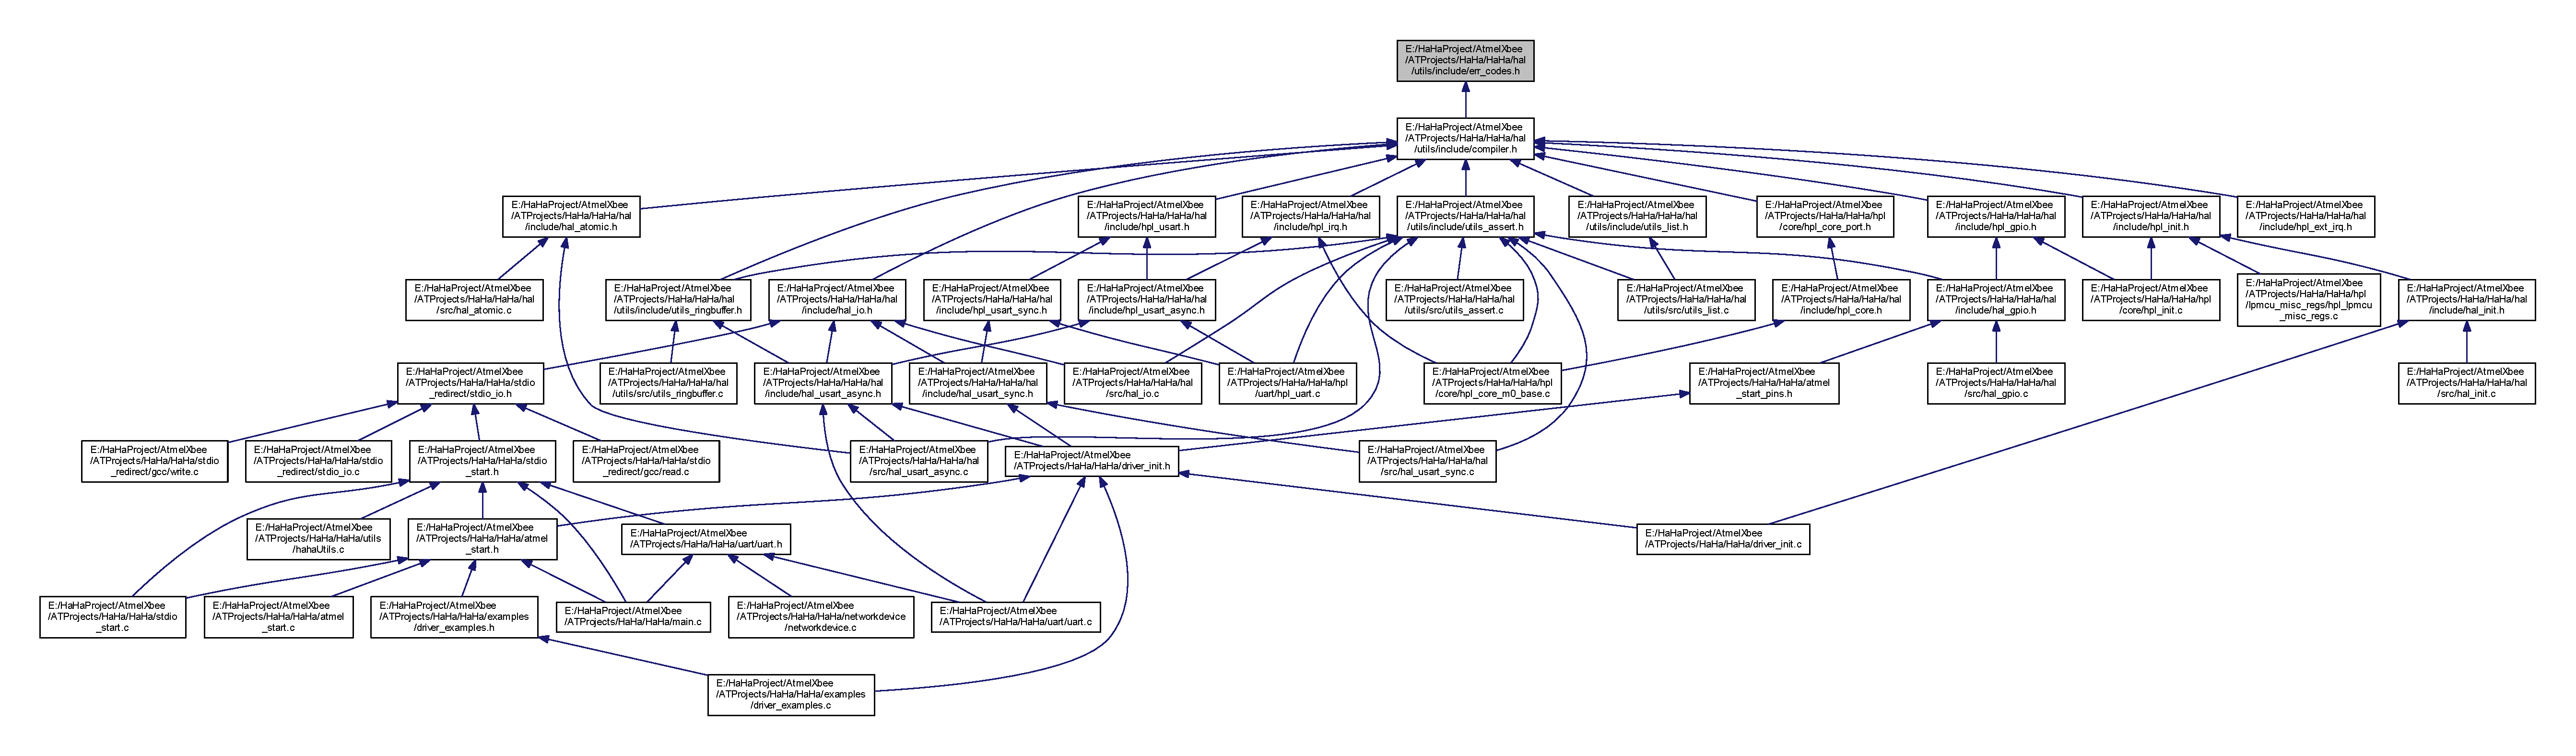
\includegraphics[width=350pt]{err__codes_8h__dep__incl}
\end{center}
\end{figure}
\subsection*{Macros}
\begin{DoxyCompactItemize}
\item 
\#define \hyperlink{err__codes_8h_aff0d3fb76f11f6e8ea4002d826bbd23c}{E\+R\+R\+\_\+\+N\+O\+NE}~0
\item 
\#define \hyperlink{err__codes_8h_a5c82bededa388cefc2819242b998394c}{E\+R\+R\+\_\+\+I\+N\+V\+A\+L\+I\+D\+\_\+\+D\+A\+TA}~-\/1
\item 
\#define \hyperlink{err__codes_8h_a417fbd9a3d16febf05f7373184bae4de}{E\+R\+R\+\_\+\+N\+O\+\_\+\+C\+H\+A\+N\+GE}~-\/2
\item 
\#define \hyperlink{err__codes_8h_a386c8c28bc424b6fe6f6c2b6e1dcba23}{E\+R\+R\+\_\+\+A\+B\+O\+R\+T\+ED}~-\/3
\item 
\#define \hyperlink{err__codes_8h_a48edef7887642685c09cf2ed00456a3d}{E\+R\+R\+\_\+\+B\+U\+SY}~-\/4
\item 
\#define \hyperlink{err__codes_8h_ad56c93536dfd8b26ab2d210b8a1113de}{E\+R\+R\+\_\+\+S\+U\+S\+P\+E\+ND}~-\/5
\item 
\#define \hyperlink{err__codes_8h_a1233473a344fe01cabc989910974a81d}{E\+R\+R\+\_\+\+IO}~-\/6
\item 
\#define \hyperlink{err__codes_8h_acbd73deafa215a97c177fda21a62885a}{E\+R\+R\+\_\+\+R\+E\+Q\+\_\+\+F\+L\+U\+S\+H\+ED}~-\/7
\item 
\#define \hyperlink{err__codes_8h_aedcf61ffa26ceba66e9995937de74d64}{E\+R\+R\+\_\+\+T\+I\+M\+E\+O\+UT}~-\/8
\item 
\#define \hyperlink{err__codes_8h_a3abd2cb76a6c61c3a1fc5fbb85077d19}{E\+R\+R\+\_\+\+B\+A\+D\+\_\+\+D\+A\+TA}~-\/9
\item 
\#define \hyperlink{err__codes_8h_a47744541258a26adfce215564d8d05f4}{E\+R\+R\+\_\+\+N\+O\+T\+\_\+\+F\+O\+U\+ND}~-\/10
\item 
\#define \hyperlink{err__codes_8h_a0ea3d8b90d53725c1fd0cae896a9a1b5}{E\+R\+R\+\_\+\+U\+N\+S\+U\+P\+P\+O\+R\+T\+E\+D\+\_\+\+D\+EV}~-\/11
\item 
\#define \hyperlink{err__codes_8h_a7e33da5071f8cb4e0815dcb47a833a5f}{E\+R\+R\+\_\+\+N\+O\+\_\+\+M\+E\+M\+O\+RY}~-\/12
\item 
\#define \hyperlink{err__codes_8h_ab892c63888ef902973432ff184874782}{E\+R\+R\+\_\+\+I\+N\+V\+A\+L\+I\+D\+\_\+\+A\+RG}~-\/13
\item 
\#define \hyperlink{err__codes_8h_aa0f603d191b9e257256b75a974495782}{E\+R\+R\+\_\+\+B\+A\+D\+\_\+\+A\+D\+D\+R\+E\+SS}~-\/14
\item 
\#define \hyperlink{err__codes_8h_a048d6235add10d8fa69e7946d3c26923}{E\+R\+R\+\_\+\+B\+A\+D\+\_\+\+F\+O\+R\+M\+AT}~-\/15
\item 
\#define \hyperlink{err__codes_8h_ab503ca75f9e38ca1c4965b7e563bf687}{E\+R\+R\+\_\+\+B\+A\+D\+\_\+\+F\+RQ}~-\/16
\item 
\#define \hyperlink{err__codes_8h_ac02954876420ed7c74bfe7a40763c19c}{E\+R\+R\+\_\+\+D\+E\+N\+I\+ED}~-\/17
\item 
\#define \hyperlink{err__codes_8h_a7a7958a21230e96a424ae9592898d194}{E\+R\+R\+\_\+\+A\+L\+R\+E\+A\+D\+Y\+\_\+\+I\+N\+I\+T\+I\+A\+L\+I\+Z\+ED}~-\/18
\item 
\#define \hyperlink{err__codes_8h_ad10b7a726bfcfbac7f7c30586e8802d0}{E\+R\+R\+\_\+\+O\+V\+E\+R\+F\+L\+OW}~-\/19
\item 
\#define \hyperlink{err__codes_8h_a8b7ec90336723b11e5d970ed8be37dc2}{E\+R\+R\+\_\+\+N\+O\+T\+\_\+\+I\+N\+I\+T\+I\+A\+L\+I\+Z\+ED}~-\/20
\item 
\#define \hyperlink{err__codes_8h_ad97d48f5082f37d0bf0f819e5d6f66b6}{E\+R\+R\+\_\+\+S\+A\+M\+P\+L\+E\+R\+A\+T\+E\+\_\+\+U\+N\+A\+V\+A\+I\+L\+A\+B\+LE}~-\/21
\item 
\#define \hyperlink{err__codes_8h_a3b6c33e86199998f22488702fedceb72}{E\+R\+R\+\_\+\+R\+E\+S\+O\+L\+U\+T\+I\+O\+N\+\_\+\+U\+N\+A\+V\+A\+I\+L\+A\+B\+LE}~-\/22
\item 
\#define \hyperlink{err__codes_8h_a0b66fe9c0b6550ff095ecdd0e6fba8fe}{E\+R\+R\+\_\+\+B\+A\+U\+D\+R\+A\+T\+E\+\_\+\+U\+N\+A\+V\+A\+I\+L\+A\+B\+LE}~-\/23
\item 
\#define \hyperlink{err__codes_8h_a2a8b4a1dbce98c5b9486964e6314ed07}{E\+R\+R\+\_\+\+P\+A\+C\+K\+E\+T\+\_\+\+C\+O\+L\+L\+I\+S\+I\+ON}~-\/24
\item 
\#define \hyperlink{err__codes_8h_ad68b6b3d07b58f9817557cdd3a8e310b}{E\+R\+R\+\_\+\+P\+R\+O\+T\+O\+C\+OL}~-\/25
\item 
\#define \hyperlink{err__codes_8h_a2891266cda7b372ab17a568fe81bbe51}{E\+R\+R\+\_\+\+P\+I\+N\+\_\+\+M\+U\+X\+\_\+\+I\+N\+V\+A\+L\+ID}~-\/26
\item 
\#define \hyperlink{err__codes_8h_a77673fbc2579e4f1f0887746e4f3a444}{E\+R\+R\+\_\+\+U\+N\+S\+U\+P\+P\+O\+R\+T\+E\+D\+\_\+\+OP}~-\/27
\item 
\#define \hyperlink{err__codes_8h_af3a4a9d084f6e3cf73ab778f82ff5e59}{E\+R\+R\+\_\+\+N\+O\+\_\+\+R\+E\+S\+O\+U\+R\+CE}~-\/28
\item 
\#define \hyperlink{err__codes_8h_a2047048fa208fc8af0415adbdd1a8058}{E\+R\+R\+\_\+\+N\+O\+T\+\_\+\+R\+E\+A\+DY}~-\/29
\item 
\#define \hyperlink{err__codes_8h_aa26fc6554da458bd012638a7020b00b6}{E\+R\+R\+\_\+\+F\+A\+I\+L\+U\+RE}~-\/30
\item 
\#define \hyperlink{err__codes_8h_a552aac7899e57c9dedebea3a2b1b340b}{E\+R\+R\+\_\+\+W\+R\+O\+N\+G\+\_\+\+L\+E\+N\+G\+TH}~-\/31
\end{DoxyCompactItemize}


\subsection{Detailed Description}
Error code definitions. 

This file defines various status codes returned by functions, indicating success or failure as well as what kind of failure.

Copyright (C) 2015 Atmel Corporation. All rights reserved.

\subsection{Macro Definition Documentation}
\mbox{\Hypertarget{err__codes_8h_a386c8c28bc424b6fe6f6c2b6e1dcba23}\label{err__codes_8h_a386c8c28bc424b6fe6f6c2b6e1dcba23}} 
\index{err\+\_\+codes.\+h@{err\+\_\+codes.\+h}!E\+R\+R\+\_\+\+A\+B\+O\+R\+T\+ED@{E\+R\+R\+\_\+\+A\+B\+O\+R\+T\+ED}}
\index{E\+R\+R\+\_\+\+A\+B\+O\+R\+T\+ED@{E\+R\+R\+\_\+\+A\+B\+O\+R\+T\+ED}!err\+\_\+codes.\+h@{err\+\_\+codes.\+h}}
\subsubsection{\texorpdfstring{E\+R\+R\+\_\+\+A\+B\+O\+R\+T\+ED}{ERR\_ABORTED}}
{\footnotesize\ttfamily \#define E\+R\+R\+\_\+\+A\+B\+O\+R\+T\+ED~-\/3}

\mbox{\Hypertarget{err__codes_8h_a7a7958a21230e96a424ae9592898d194}\label{err__codes_8h_a7a7958a21230e96a424ae9592898d194}} 
\index{err\+\_\+codes.\+h@{err\+\_\+codes.\+h}!E\+R\+R\+\_\+\+A\+L\+R\+E\+A\+D\+Y\+\_\+\+I\+N\+I\+T\+I\+A\+L\+I\+Z\+ED@{E\+R\+R\+\_\+\+A\+L\+R\+E\+A\+D\+Y\+\_\+\+I\+N\+I\+T\+I\+A\+L\+I\+Z\+ED}}
\index{E\+R\+R\+\_\+\+A\+L\+R\+E\+A\+D\+Y\+\_\+\+I\+N\+I\+T\+I\+A\+L\+I\+Z\+ED@{E\+R\+R\+\_\+\+A\+L\+R\+E\+A\+D\+Y\+\_\+\+I\+N\+I\+T\+I\+A\+L\+I\+Z\+ED}!err\+\_\+codes.\+h@{err\+\_\+codes.\+h}}
\subsubsection{\texorpdfstring{E\+R\+R\+\_\+\+A\+L\+R\+E\+A\+D\+Y\+\_\+\+I\+N\+I\+T\+I\+A\+L\+I\+Z\+ED}{ERR\_ALREADY\_INITIALIZED}}
{\footnotesize\ttfamily \#define E\+R\+R\+\_\+\+A\+L\+R\+E\+A\+D\+Y\+\_\+\+I\+N\+I\+T\+I\+A\+L\+I\+Z\+ED~-\/18}

\mbox{\Hypertarget{err__codes_8h_aa0f603d191b9e257256b75a974495782}\label{err__codes_8h_aa0f603d191b9e257256b75a974495782}} 
\index{err\+\_\+codes.\+h@{err\+\_\+codes.\+h}!E\+R\+R\+\_\+\+B\+A\+D\+\_\+\+A\+D\+D\+R\+E\+SS@{E\+R\+R\+\_\+\+B\+A\+D\+\_\+\+A\+D\+D\+R\+E\+SS}}
\index{E\+R\+R\+\_\+\+B\+A\+D\+\_\+\+A\+D\+D\+R\+E\+SS@{E\+R\+R\+\_\+\+B\+A\+D\+\_\+\+A\+D\+D\+R\+E\+SS}!err\+\_\+codes.\+h@{err\+\_\+codes.\+h}}
\subsubsection{\texorpdfstring{E\+R\+R\+\_\+\+B\+A\+D\+\_\+\+A\+D\+D\+R\+E\+SS}{ERR\_BAD\_ADDRESS}}
{\footnotesize\ttfamily \#define E\+R\+R\+\_\+\+B\+A\+D\+\_\+\+A\+D\+D\+R\+E\+SS~-\/14}

\mbox{\Hypertarget{err__codes_8h_a3abd2cb76a6c61c3a1fc5fbb85077d19}\label{err__codes_8h_a3abd2cb76a6c61c3a1fc5fbb85077d19}} 
\index{err\+\_\+codes.\+h@{err\+\_\+codes.\+h}!E\+R\+R\+\_\+\+B\+A\+D\+\_\+\+D\+A\+TA@{E\+R\+R\+\_\+\+B\+A\+D\+\_\+\+D\+A\+TA}}
\index{E\+R\+R\+\_\+\+B\+A\+D\+\_\+\+D\+A\+TA@{E\+R\+R\+\_\+\+B\+A\+D\+\_\+\+D\+A\+TA}!err\+\_\+codes.\+h@{err\+\_\+codes.\+h}}
\subsubsection{\texorpdfstring{E\+R\+R\+\_\+\+B\+A\+D\+\_\+\+D\+A\+TA}{ERR\_BAD\_DATA}}
{\footnotesize\ttfamily \#define E\+R\+R\+\_\+\+B\+A\+D\+\_\+\+D\+A\+TA~-\/9}

\mbox{\Hypertarget{err__codes_8h_a048d6235add10d8fa69e7946d3c26923}\label{err__codes_8h_a048d6235add10d8fa69e7946d3c26923}} 
\index{err\+\_\+codes.\+h@{err\+\_\+codes.\+h}!E\+R\+R\+\_\+\+B\+A\+D\+\_\+\+F\+O\+R\+M\+AT@{E\+R\+R\+\_\+\+B\+A\+D\+\_\+\+F\+O\+R\+M\+AT}}
\index{E\+R\+R\+\_\+\+B\+A\+D\+\_\+\+F\+O\+R\+M\+AT@{E\+R\+R\+\_\+\+B\+A\+D\+\_\+\+F\+O\+R\+M\+AT}!err\+\_\+codes.\+h@{err\+\_\+codes.\+h}}
\subsubsection{\texorpdfstring{E\+R\+R\+\_\+\+B\+A\+D\+\_\+\+F\+O\+R\+M\+AT}{ERR\_BAD\_FORMAT}}
{\footnotesize\ttfamily \#define E\+R\+R\+\_\+\+B\+A\+D\+\_\+\+F\+O\+R\+M\+AT~-\/15}

\mbox{\Hypertarget{err__codes_8h_ab503ca75f9e38ca1c4965b7e563bf687}\label{err__codes_8h_ab503ca75f9e38ca1c4965b7e563bf687}} 
\index{err\+\_\+codes.\+h@{err\+\_\+codes.\+h}!E\+R\+R\+\_\+\+B\+A\+D\+\_\+\+F\+RQ@{E\+R\+R\+\_\+\+B\+A\+D\+\_\+\+F\+RQ}}
\index{E\+R\+R\+\_\+\+B\+A\+D\+\_\+\+F\+RQ@{E\+R\+R\+\_\+\+B\+A\+D\+\_\+\+F\+RQ}!err\+\_\+codes.\+h@{err\+\_\+codes.\+h}}
\subsubsection{\texorpdfstring{E\+R\+R\+\_\+\+B\+A\+D\+\_\+\+F\+RQ}{ERR\_BAD\_FRQ}}
{\footnotesize\ttfamily \#define E\+R\+R\+\_\+\+B\+A\+D\+\_\+\+F\+RQ~-\/16}

\mbox{\Hypertarget{err__codes_8h_a0b66fe9c0b6550ff095ecdd0e6fba8fe}\label{err__codes_8h_a0b66fe9c0b6550ff095ecdd0e6fba8fe}} 
\index{err\+\_\+codes.\+h@{err\+\_\+codes.\+h}!E\+R\+R\+\_\+\+B\+A\+U\+D\+R\+A\+T\+E\+\_\+\+U\+N\+A\+V\+A\+I\+L\+A\+B\+LE@{E\+R\+R\+\_\+\+B\+A\+U\+D\+R\+A\+T\+E\+\_\+\+U\+N\+A\+V\+A\+I\+L\+A\+B\+LE}}
\index{E\+R\+R\+\_\+\+B\+A\+U\+D\+R\+A\+T\+E\+\_\+\+U\+N\+A\+V\+A\+I\+L\+A\+B\+LE@{E\+R\+R\+\_\+\+B\+A\+U\+D\+R\+A\+T\+E\+\_\+\+U\+N\+A\+V\+A\+I\+L\+A\+B\+LE}!err\+\_\+codes.\+h@{err\+\_\+codes.\+h}}
\subsubsection{\texorpdfstring{E\+R\+R\+\_\+\+B\+A\+U\+D\+R\+A\+T\+E\+\_\+\+U\+N\+A\+V\+A\+I\+L\+A\+B\+LE}{ERR\_BAUDRATE\_UNAVAILABLE}}
{\footnotesize\ttfamily \#define E\+R\+R\+\_\+\+B\+A\+U\+D\+R\+A\+T\+E\+\_\+\+U\+N\+A\+V\+A\+I\+L\+A\+B\+LE~-\/23}

\mbox{\Hypertarget{err__codes_8h_a48edef7887642685c09cf2ed00456a3d}\label{err__codes_8h_a48edef7887642685c09cf2ed00456a3d}} 
\index{err\+\_\+codes.\+h@{err\+\_\+codes.\+h}!E\+R\+R\+\_\+\+B\+U\+SY@{E\+R\+R\+\_\+\+B\+U\+SY}}
\index{E\+R\+R\+\_\+\+B\+U\+SY@{E\+R\+R\+\_\+\+B\+U\+SY}!err\+\_\+codes.\+h@{err\+\_\+codes.\+h}}
\subsubsection{\texorpdfstring{E\+R\+R\+\_\+\+B\+U\+SY}{ERR\_BUSY}}
{\footnotesize\ttfamily \#define E\+R\+R\+\_\+\+B\+U\+SY~-\/4}

\mbox{\Hypertarget{err__codes_8h_ac02954876420ed7c74bfe7a40763c19c}\label{err__codes_8h_ac02954876420ed7c74bfe7a40763c19c}} 
\index{err\+\_\+codes.\+h@{err\+\_\+codes.\+h}!E\+R\+R\+\_\+\+D\+E\+N\+I\+ED@{E\+R\+R\+\_\+\+D\+E\+N\+I\+ED}}
\index{E\+R\+R\+\_\+\+D\+E\+N\+I\+ED@{E\+R\+R\+\_\+\+D\+E\+N\+I\+ED}!err\+\_\+codes.\+h@{err\+\_\+codes.\+h}}
\subsubsection{\texorpdfstring{E\+R\+R\+\_\+\+D\+E\+N\+I\+ED}{ERR\_DENIED}}
{\footnotesize\ttfamily \#define E\+R\+R\+\_\+\+D\+E\+N\+I\+ED~-\/17}

\mbox{\Hypertarget{err__codes_8h_aa26fc6554da458bd012638a7020b00b6}\label{err__codes_8h_aa26fc6554da458bd012638a7020b00b6}} 
\index{err\+\_\+codes.\+h@{err\+\_\+codes.\+h}!E\+R\+R\+\_\+\+F\+A\+I\+L\+U\+RE@{E\+R\+R\+\_\+\+F\+A\+I\+L\+U\+RE}}
\index{E\+R\+R\+\_\+\+F\+A\+I\+L\+U\+RE@{E\+R\+R\+\_\+\+F\+A\+I\+L\+U\+RE}!err\+\_\+codes.\+h@{err\+\_\+codes.\+h}}
\subsubsection{\texorpdfstring{E\+R\+R\+\_\+\+F\+A\+I\+L\+U\+RE}{ERR\_FAILURE}}
{\footnotesize\ttfamily \#define E\+R\+R\+\_\+\+F\+A\+I\+L\+U\+RE~-\/30}

\mbox{\Hypertarget{err__codes_8h_ab892c63888ef902973432ff184874782}\label{err__codes_8h_ab892c63888ef902973432ff184874782}} 
\index{err\+\_\+codes.\+h@{err\+\_\+codes.\+h}!E\+R\+R\+\_\+\+I\+N\+V\+A\+L\+I\+D\+\_\+\+A\+RG@{E\+R\+R\+\_\+\+I\+N\+V\+A\+L\+I\+D\+\_\+\+A\+RG}}
\index{E\+R\+R\+\_\+\+I\+N\+V\+A\+L\+I\+D\+\_\+\+A\+RG@{E\+R\+R\+\_\+\+I\+N\+V\+A\+L\+I\+D\+\_\+\+A\+RG}!err\+\_\+codes.\+h@{err\+\_\+codes.\+h}}
\subsubsection{\texorpdfstring{E\+R\+R\+\_\+\+I\+N\+V\+A\+L\+I\+D\+\_\+\+A\+RG}{ERR\_INVALID\_ARG}}
{\footnotesize\ttfamily \#define E\+R\+R\+\_\+\+I\+N\+V\+A\+L\+I\+D\+\_\+\+A\+RG~-\/13}

\mbox{\Hypertarget{err__codes_8h_a5c82bededa388cefc2819242b998394c}\label{err__codes_8h_a5c82bededa388cefc2819242b998394c}} 
\index{err\+\_\+codes.\+h@{err\+\_\+codes.\+h}!E\+R\+R\+\_\+\+I\+N\+V\+A\+L\+I\+D\+\_\+\+D\+A\+TA@{E\+R\+R\+\_\+\+I\+N\+V\+A\+L\+I\+D\+\_\+\+D\+A\+TA}}
\index{E\+R\+R\+\_\+\+I\+N\+V\+A\+L\+I\+D\+\_\+\+D\+A\+TA@{E\+R\+R\+\_\+\+I\+N\+V\+A\+L\+I\+D\+\_\+\+D\+A\+TA}!err\+\_\+codes.\+h@{err\+\_\+codes.\+h}}
\subsubsection{\texorpdfstring{E\+R\+R\+\_\+\+I\+N\+V\+A\+L\+I\+D\+\_\+\+D\+A\+TA}{ERR\_INVALID\_DATA}}
{\footnotesize\ttfamily \#define E\+R\+R\+\_\+\+I\+N\+V\+A\+L\+I\+D\+\_\+\+D\+A\+TA~-\/1}

\mbox{\Hypertarget{err__codes_8h_a1233473a344fe01cabc989910974a81d}\label{err__codes_8h_a1233473a344fe01cabc989910974a81d}} 
\index{err\+\_\+codes.\+h@{err\+\_\+codes.\+h}!E\+R\+R\+\_\+\+IO@{E\+R\+R\+\_\+\+IO}}
\index{E\+R\+R\+\_\+\+IO@{E\+R\+R\+\_\+\+IO}!err\+\_\+codes.\+h@{err\+\_\+codes.\+h}}
\subsubsection{\texorpdfstring{E\+R\+R\+\_\+\+IO}{ERR\_IO}}
{\footnotesize\ttfamily \#define E\+R\+R\+\_\+\+IO~-\/6}

\mbox{\Hypertarget{err__codes_8h_a417fbd9a3d16febf05f7373184bae4de}\label{err__codes_8h_a417fbd9a3d16febf05f7373184bae4de}} 
\index{err\+\_\+codes.\+h@{err\+\_\+codes.\+h}!E\+R\+R\+\_\+\+N\+O\+\_\+\+C\+H\+A\+N\+GE@{E\+R\+R\+\_\+\+N\+O\+\_\+\+C\+H\+A\+N\+GE}}
\index{E\+R\+R\+\_\+\+N\+O\+\_\+\+C\+H\+A\+N\+GE@{E\+R\+R\+\_\+\+N\+O\+\_\+\+C\+H\+A\+N\+GE}!err\+\_\+codes.\+h@{err\+\_\+codes.\+h}}
\subsubsection{\texorpdfstring{E\+R\+R\+\_\+\+N\+O\+\_\+\+C\+H\+A\+N\+GE}{ERR\_NO\_CHANGE}}
{\footnotesize\ttfamily \#define E\+R\+R\+\_\+\+N\+O\+\_\+\+C\+H\+A\+N\+GE~-\/2}

\mbox{\Hypertarget{err__codes_8h_a7e33da5071f8cb4e0815dcb47a833a5f}\label{err__codes_8h_a7e33da5071f8cb4e0815dcb47a833a5f}} 
\index{err\+\_\+codes.\+h@{err\+\_\+codes.\+h}!E\+R\+R\+\_\+\+N\+O\+\_\+\+M\+E\+M\+O\+RY@{E\+R\+R\+\_\+\+N\+O\+\_\+\+M\+E\+M\+O\+RY}}
\index{E\+R\+R\+\_\+\+N\+O\+\_\+\+M\+E\+M\+O\+RY@{E\+R\+R\+\_\+\+N\+O\+\_\+\+M\+E\+M\+O\+RY}!err\+\_\+codes.\+h@{err\+\_\+codes.\+h}}
\subsubsection{\texorpdfstring{E\+R\+R\+\_\+\+N\+O\+\_\+\+M\+E\+M\+O\+RY}{ERR\_NO\_MEMORY}}
{\footnotesize\ttfamily \#define E\+R\+R\+\_\+\+N\+O\+\_\+\+M\+E\+M\+O\+RY~-\/12}

\mbox{\Hypertarget{err__codes_8h_af3a4a9d084f6e3cf73ab778f82ff5e59}\label{err__codes_8h_af3a4a9d084f6e3cf73ab778f82ff5e59}} 
\index{err\+\_\+codes.\+h@{err\+\_\+codes.\+h}!E\+R\+R\+\_\+\+N\+O\+\_\+\+R\+E\+S\+O\+U\+R\+CE@{E\+R\+R\+\_\+\+N\+O\+\_\+\+R\+E\+S\+O\+U\+R\+CE}}
\index{E\+R\+R\+\_\+\+N\+O\+\_\+\+R\+E\+S\+O\+U\+R\+CE@{E\+R\+R\+\_\+\+N\+O\+\_\+\+R\+E\+S\+O\+U\+R\+CE}!err\+\_\+codes.\+h@{err\+\_\+codes.\+h}}
\subsubsection{\texorpdfstring{E\+R\+R\+\_\+\+N\+O\+\_\+\+R\+E\+S\+O\+U\+R\+CE}{ERR\_NO\_RESOURCE}}
{\footnotesize\ttfamily \#define E\+R\+R\+\_\+\+N\+O\+\_\+\+R\+E\+S\+O\+U\+R\+CE~-\/28}

\mbox{\Hypertarget{err__codes_8h_aff0d3fb76f11f6e8ea4002d826bbd23c}\label{err__codes_8h_aff0d3fb76f11f6e8ea4002d826bbd23c}} 
\index{err\+\_\+codes.\+h@{err\+\_\+codes.\+h}!E\+R\+R\+\_\+\+N\+O\+NE@{E\+R\+R\+\_\+\+N\+O\+NE}}
\index{E\+R\+R\+\_\+\+N\+O\+NE@{E\+R\+R\+\_\+\+N\+O\+NE}!err\+\_\+codes.\+h@{err\+\_\+codes.\+h}}
\subsubsection{\texorpdfstring{E\+R\+R\+\_\+\+N\+O\+NE}{ERR\_NONE}}
{\footnotesize\ttfamily \#define E\+R\+R\+\_\+\+N\+O\+NE~0}

\mbox{\Hypertarget{err__codes_8h_a47744541258a26adfce215564d8d05f4}\label{err__codes_8h_a47744541258a26adfce215564d8d05f4}} 
\index{err\+\_\+codes.\+h@{err\+\_\+codes.\+h}!E\+R\+R\+\_\+\+N\+O\+T\+\_\+\+F\+O\+U\+ND@{E\+R\+R\+\_\+\+N\+O\+T\+\_\+\+F\+O\+U\+ND}}
\index{E\+R\+R\+\_\+\+N\+O\+T\+\_\+\+F\+O\+U\+ND@{E\+R\+R\+\_\+\+N\+O\+T\+\_\+\+F\+O\+U\+ND}!err\+\_\+codes.\+h@{err\+\_\+codes.\+h}}
\subsubsection{\texorpdfstring{E\+R\+R\+\_\+\+N\+O\+T\+\_\+\+F\+O\+U\+ND}{ERR\_NOT\_FOUND}}
{\footnotesize\ttfamily \#define E\+R\+R\+\_\+\+N\+O\+T\+\_\+\+F\+O\+U\+ND~-\/10}

\mbox{\Hypertarget{err__codes_8h_a8b7ec90336723b11e5d970ed8be37dc2}\label{err__codes_8h_a8b7ec90336723b11e5d970ed8be37dc2}} 
\index{err\+\_\+codes.\+h@{err\+\_\+codes.\+h}!E\+R\+R\+\_\+\+N\+O\+T\+\_\+\+I\+N\+I\+T\+I\+A\+L\+I\+Z\+ED@{E\+R\+R\+\_\+\+N\+O\+T\+\_\+\+I\+N\+I\+T\+I\+A\+L\+I\+Z\+ED}}
\index{E\+R\+R\+\_\+\+N\+O\+T\+\_\+\+I\+N\+I\+T\+I\+A\+L\+I\+Z\+ED@{E\+R\+R\+\_\+\+N\+O\+T\+\_\+\+I\+N\+I\+T\+I\+A\+L\+I\+Z\+ED}!err\+\_\+codes.\+h@{err\+\_\+codes.\+h}}
\subsubsection{\texorpdfstring{E\+R\+R\+\_\+\+N\+O\+T\+\_\+\+I\+N\+I\+T\+I\+A\+L\+I\+Z\+ED}{ERR\_NOT\_INITIALIZED}}
{\footnotesize\ttfamily \#define E\+R\+R\+\_\+\+N\+O\+T\+\_\+\+I\+N\+I\+T\+I\+A\+L\+I\+Z\+ED~-\/20}

\mbox{\Hypertarget{err__codes_8h_a2047048fa208fc8af0415adbdd1a8058}\label{err__codes_8h_a2047048fa208fc8af0415adbdd1a8058}} 
\index{err\+\_\+codes.\+h@{err\+\_\+codes.\+h}!E\+R\+R\+\_\+\+N\+O\+T\+\_\+\+R\+E\+A\+DY@{E\+R\+R\+\_\+\+N\+O\+T\+\_\+\+R\+E\+A\+DY}}
\index{E\+R\+R\+\_\+\+N\+O\+T\+\_\+\+R\+E\+A\+DY@{E\+R\+R\+\_\+\+N\+O\+T\+\_\+\+R\+E\+A\+DY}!err\+\_\+codes.\+h@{err\+\_\+codes.\+h}}
\subsubsection{\texorpdfstring{E\+R\+R\+\_\+\+N\+O\+T\+\_\+\+R\+E\+A\+DY}{ERR\_NOT\_READY}}
{\footnotesize\ttfamily \#define E\+R\+R\+\_\+\+N\+O\+T\+\_\+\+R\+E\+A\+DY~-\/29}

\mbox{\Hypertarget{err__codes_8h_ad10b7a726bfcfbac7f7c30586e8802d0}\label{err__codes_8h_ad10b7a726bfcfbac7f7c30586e8802d0}} 
\index{err\+\_\+codes.\+h@{err\+\_\+codes.\+h}!E\+R\+R\+\_\+\+O\+V\+E\+R\+F\+L\+OW@{E\+R\+R\+\_\+\+O\+V\+E\+R\+F\+L\+OW}}
\index{E\+R\+R\+\_\+\+O\+V\+E\+R\+F\+L\+OW@{E\+R\+R\+\_\+\+O\+V\+E\+R\+F\+L\+OW}!err\+\_\+codes.\+h@{err\+\_\+codes.\+h}}
\subsubsection{\texorpdfstring{E\+R\+R\+\_\+\+O\+V\+E\+R\+F\+L\+OW}{ERR\_OVERFLOW}}
{\footnotesize\ttfamily \#define E\+R\+R\+\_\+\+O\+V\+E\+R\+F\+L\+OW~-\/19}

\mbox{\Hypertarget{err__codes_8h_a2a8b4a1dbce98c5b9486964e6314ed07}\label{err__codes_8h_a2a8b4a1dbce98c5b9486964e6314ed07}} 
\index{err\+\_\+codes.\+h@{err\+\_\+codes.\+h}!E\+R\+R\+\_\+\+P\+A\+C\+K\+E\+T\+\_\+\+C\+O\+L\+L\+I\+S\+I\+ON@{E\+R\+R\+\_\+\+P\+A\+C\+K\+E\+T\+\_\+\+C\+O\+L\+L\+I\+S\+I\+ON}}
\index{E\+R\+R\+\_\+\+P\+A\+C\+K\+E\+T\+\_\+\+C\+O\+L\+L\+I\+S\+I\+ON@{E\+R\+R\+\_\+\+P\+A\+C\+K\+E\+T\+\_\+\+C\+O\+L\+L\+I\+S\+I\+ON}!err\+\_\+codes.\+h@{err\+\_\+codes.\+h}}
\subsubsection{\texorpdfstring{E\+R\+R\+\_\+\+P\+A\+C\+K\+E\+T\+\_\+\+C\+O\+L\+L\+I\+S\+I\+ON}{ERR\_PACKET\_COLLISION}}
{\footnotesize\ttfamily \#define E\+R\+R\+\_\+\+P\+A\+C\+K\+E\+T\+\_\+\+C\+O\+L\+L\+I\+S\+I\+ON~-\/24}

\mbox{\Hypertarget{err__codes_8h_a2891266cda7b372ab17a568fe81bbe51}\label{err__codes_8h_a2891266cda7b372ab17a568fe81bbe51}} 
\index{err\+\_\+codes.\+h@{err\+\_\+codes.\+h}!E\+R\+R\+\_\+\+P\+I\+N\+\_\+\+M\+U\+X\+\_\+\+I\+N\+V\+A\+L\+ID@{E\+R\+R\+\_\+\+P\+I\+N\+\_\+\+M\+U\+X\+\_\+\+I\+N\+V\+A\+L\+ID}}
\index{E\+R\+R\+\_\+\+P\+I\+N\+\_\+\+M\+U\+X\+\_\+\+I\+N\+V\+A\+L\+ID@{E\+R\+R\+\_\+\+P\+I\+N\+\_\+\+M\+U\+X\+\_\+\+I\+N\+V\+A\+L\+ID}!err\+\_\+codes.\+h@{err\+\_\+codes.\+h}}
\subsubsection{\texorpdfstring{E\+R\+R\+\_\+\+P\+I\+N\+\_\+\+M\+U\+X\+\_\+\+I\+N\+V\+A\+L\+ID}{ERR\_PIN\_MUX\_INVALID}}
{\footnotesize\ttfamily \#define E\+R\+R\+\_\+\+P\+I\+N\+\_\+\+M\+U\+X\+\_\+\+I\+N\+V\+A\+L\+ID~-\/26}

\mbox{\Hypertarget{err__codes_8h_ad68b6b3d07b58f9817557cdd3a8e310b}\label{err__codes_8h_ad68b6b3d07b58f9817557cdd3a8e310b}} 
\index{err\+\_\+codes.\+h@{err\+\_\+codes.\+h}!E\+R\+R\+\_\+\+P\+R\+O\+T\+O\+C\+OL@{E\+R\+R\+\_\+\+P\+R\+O\+T\+O\+C\+OL}}
\index{E\+R\+R\+\_\+\+P\+R\+O\+T\+O\+C\+OL@{E\+R\+R\+\_\+\+P\+R\+O\+T\+O\+C\+OL}!err\+\_\+codes.\+h@{err\+\_\+codes.\+h}}
\subsubsection{\texorpdfstring{E\+R\+R\+\_\+\+P\+R\+O\+T\+O\+C\+OL}{ERR\_PROTOCOL}}
{\footnotesize\ttfamily \#define E\+R\+R\+\_\+\+P\+R\+O\+T\+O\+C\+OL~-\/25}

\mbox{\Hypertarget{err__codes_8h_acbd73deafa215a97c177fda21a62885a}\label{err__codes_8h_acbd73deafa215a97c177fda21a62885a}} 
\index{err\+\_\+codes.\+h@{err\+\_\+codes.\+h}!E\+R\+R\+\_\+\+R\+E\+Q\+\_\+\+F\+L\+U\+S\+H\+ED@{E\+R\+R\+\_\+\+R\+E\+Q\+\_\+\+F\+L\+U\+S\+H\+ED}}
\index{E\+R\+R\+\_\+\+R\+E\+Q\+\_\+\+F\+L\+U\+S\+H\+ED@{E\+R\+R\+\_\+\+R\+E\+Q\+\_\+\+F\+L\+U\+S\+H\+ED}!err\+\_\+codes.\+h@{err\+\_\+codes.\+h}}
\subsubsection{\texorpdfstring{E\+R\+R\+\_\+\+R\+E\+Q\+\_\+\+F\+L\+U\+S\+H\+ED}{ERR\_REQ\_FLUSHED}}
{\footnotesize\ttfamily \#define E\+R\+R\+\_\+\+R\+E\+Q\+\_\+\+F\+L\+U\+S\+H\+ED~-\/7}

\mbox{\Hypertarget{err__codes_8h_a3b6c33e86199998f22488702fedceb72}\label{err__codes_8h_a3b6c33e86199998f22488702fedceb72}} 
\index{err\+\_\+codes.\+h@{err\+\_\+codes.\+h}!E\+R\+R\+\_\+\+R\+E\+S\+O\+L\+U\+T\+I\+O\+N\+\_\+\+U\+N\+A\+V\+A\+I\+L\+A\+B\+LE@{E\+R\+R\+\_\+\+R\+E\+S\+O\+L\+U\+T\+I\+O\+N\+\_\+\+U\+N\+A\+V\+A\+I\+L\+A\+B\+LE}}
\index{E\+R\+R\+\_\+\+R\+E\+S\+O\+L\+U\+T\+I\+O\+N\+\_\+\+U\+N\+A\+V\+A\+I\+L\+A\+B\+LE@{E\+R\+R\+\_\+\+R\+E\+S\+O\+L\+U\+T\+I\+O\+N\+\_\+\+U\+N\+A\+V\+A\+I\+L\+A\+B\+LE}!err\+\_\+codes.\+h@{err\+\_\+codes.\+h}}
\subsubsection{\texorpdfstring{E\+R\+R\+\_\+\+R\+E\+S\+O\+L\+U\+T\+I\+O\+N\+\_\+\+U\+N\+A\+V\+A\+I\+L\+A\+B\+LE}{ERR\_RESOLUTION\_UNAVAILABLE}}
{\footnotesize\ttfamily \#define E\+R\+R\+\_\+\+R\+E\+S\+O\+L\+U\+T\+I\+O\+N\+\_\+\+U\+N\+A\+V\+A\+I\+L\+A\+B\+LE~-\/22}

\mbox{\Hypertarget{err__codes_8h_ad97d48f5082f37d0bf0f819e5d6f66b6}\label{err__codes_8h_ad97d48f5082f37d0bf0f819e5d6f66b6}} 
\index{err\+\_\+codes.\+h@{err\+\_\+codes.\+h}!E\+R\+R\+\_\+\+S\+A\+M\+P\+L\+E\+R\+A\+T\+E\+\_\+\+U\+N\+A\+V\+A\+I\+L\+A\+B\+LE@{E\+R\+R\+\_\+\+S\+A\+M\+P\+L\+E\+R\+A\+T\+E\+\_\+\+U\+N\+A\+V\+A\+I\+L\+A\+B\+LE}}
\index{E\+R\+R\+\_\+\+S\+A\+M\+P\+L\+E\+R\+A\+T\+E\+\_\+\+U\+N\+A\+V\+A\+I\+L\+A\+B\+LE@{E\+R\+R\+\_\+\+S\+A\+M\+P\+L\+E\+R\+A\+T\+E\+\_\+\+U\+N\+A\+V\+A\+I\+L\+A\+B\+LE}!err\+\_\+codes.\+h@{err\+\_\+codes.\+h}}
\subsubsection{\texorpdfstring{E\+R\+R\+\_\+\+S\+A\+M\+P\+L\+E\+R\+A\+T\+E\+\_\+\+U\+N\+A\+V\+A\+I\+L\+A\+B\+LE}{ERR\_SAMPLERATE\_UNAVAILABLE}}
{\footnotesize\ttfamily \#define E\+R\+R\+\_\+\+S\+A\+M\+P\+L\+E\+R\+A\+T\+E\+\_\+\+U\+N\+A\+V\+A\+I\+L\+A\+B\+LE~-\/21}

\mbox{\Hypertarget{err__codes_8h_ad56c93536dfd8b26ab2d210b8a1113de}\label{err__codes_8h_ad56c93536dfd8b26ab2d210b8a1113de}} 
\index{err\+\_\+codes.\+h@{err\+\_\+codes.\+h}!E\+R\+R\+\_\+\+S\+U\+S\+P\+E\+ND@{E\+R\+R\+\_\+\+S\+U\+S\+P\+E\+ND}}
\index{E\+R\+R\+\_\+\+S\+U\+S\+P\+E\+ND@{E\+R\+R\+\_\+\+S\+U\+S\+P\+E\+ND}!err\+\_\+codes.\+h@{err\+\_\+codes.\+h}}
\subsubsection{\texorpdfstring{E\+R\+R\+\_\+\+S\+U\+S\+P\+E\+ND}{ERR\_SUSPEND}}
{\footnotesize\ttfamily \#define E\+R\+R\+\_\+\+S\+U\+S\+P\+E\+ND~-\/5}

\mbox{\Hypertarget{err__codes_8h_aedcf61ffa26ceba66e9995937de74d64}\label{err__codes_8h_aedcf61ffa26ceba66e9995937de74d64}} 
\index{err\+\_\+codes.\+h@{err\+\_\+codes.\+h}!E\+R\+R\+\_\+\+T\+I\+M\+E\+O\+UT@{E\+R\+R\+\_\+\+T\+I\+M\+E\+O\+UT}}
\index{E\+R\+R\+\_\+\+T\+I\+M\+E\+O\+UT@{E\+R\+R\+\_\+\+T\+I\+M\+E\+O\+UT}!err\+\_\+codes.\+h@{err\+\_\+codes.\+h}}
\subsubsection{\texorpdfstring{E\+R\+R\+\_\+\+T\+I\+M\+E\+O\+UT}{ERR\_TIMEOUT}}
{\footnotesize\ttfamily \#define E\+R\+R\+\_\+\+T\+I\+M\+E\+O\+UT~-\/8}

\mbox{\Hypertarget{err__codes_8h_a0ea3d8b90d53725c1fd0cae896a9a1b5}\label{err__codes_8h_a0ea3d8b90d53725c1fd0cae896a9a1b5}} 
\index{err\+\_\+codes.\+h@{err\+\_\+codes.\+h}!E\+R\+R\+\_\+\+U\+N\+S\+U\+P\+P\+O\+R\+T\+E\+D\+\_\+\+D\+EV@{E\+R\+R\+\_\+\+U\+N\+S\+U\+P\+P\+O\+R\+T\+E\+D\+\_\+\+D\+EV}}
\index{E\+R\+R\+\_\+\+U\+N\+S\+U\+P\+P\+O\+R\+T\+E\+D\+\_\+\+D\+EV@{E\+R\+R\+\_\+\+U\+N\+S\+U\+P\+P\+O\+R\+T\+E\+D\+\_\+\+D\+EV}!err\+\_\+codes.\+h@{err\+\_\+codes.\+h}}
\subsubsection{\texorpdfstring{E\+R\+R\+\_\+\+U\+N\+S\+U\+P\+P\+O\+R\+T\+E\+D\+\_\+\+D\+EV}{ERR\_UNSUPPORTED\_DEV}}
{\footnotesize\ttfamily \#define E\+R\+R\+\_\+\+U\+N\+S\+U\+P\+P\+O\+R\+T\+E\+D\+\_\+\+D\+EV~-\/11}

\mbox{\Hypertarget{err__codes_8h_a77673fbc2579e4f1f0887746e4f3a444}\label{err__codes_8h_a77673fbc2579e4f1f0887746e4f3a444}} 
\index{err\+\_\+codes.\+h@{err\+\_\+codes.\+h}!E\+R\+R\+\_\+\+U\+N\+S\+U\+P\+P\+O\+R\+T\+E\+D\+\_\+\+OP@{E\+R\+R\+\_\+\+U\+N\+S\+U\+P\+P\+O\+R\+T\+E\+D\+\_\+\+OP}}
\index{E\+R\+R\+\_\+\+U\+N\+S\+U\+P\+P\+O\+R\+T\+E\+D\+\_\+\+OP@{E\+R\+R\+\_\+\+U\+N\+S\+U\+P\+P\+O\+R\+T\+E\+D\+\_\+\+OP}!err\+\_\+codes.\+h@{err\+\_\+codes.\+h}}
\subsubsection{\texorpdfstring{E\+R\+R\+\_\+\+U\+N\+S\+U\+P\+P\+O\+R\+T\+E\+D\+\_\+\+OP}{ERR\_UNSUPPORTED\_OP}}
{\footnotesize\ttfamily \#define E\+R\+R\+\_\+\+U\+N\+S\+U\+P\+P\+O\+R\+T\+E\+D\+\_\+\+OP~-\/27}

\mbox{\Hypertarget{err__codes_8h_a552aac7899e57c9dedebea3a2b1b340b}\label{err__codes_8h_a552aac7899e57c9dedebea3a2b1b340b}} 
\index{err\+\_\+codes.\+h@{err\+\_\+codes.\+h}!E\+R\+R\+\_\+\+W\+R\+O\+N\+G\+\_\+\+L\+E\+N\+G\+TH@{E\+R\+R\+\_\+\+W\+R\+O\+N\+G\+\_\+\+L\+E\+N\+G\+TH}}
\index{E\+R\+R\+\_\+\+W\+R\+O\+N\+G\+\_\+\+L\+E\+N\+G\+TH@{E\+R\+R\+\_\+\+W\+R\+O\+N\+G\+\_\+\+L\+E\+N\+G\+TH}!err\+\_\+codes.\+h@{err\+\_\+codes.\+h}}
\subsubsection{\texorpdfstring{E\+R\+R\+\_\+\+W\+R\+O\+N\+G\+\_\+\+L\+E\+N\+G\+TH}{ERR\_WRONG\_LENGTH}}
{\footnotesize\ttfamily \#define E\+R\+R\+\_\+\+W\+R\+O\+N\+G\+\_\+\+L\+E\+N\+G\+TH~-\/31}


\hypertarget{parts_8h}{}\section{E\+:/\+Ha\+Ha\+Project/\+Atmel\+Xbee/\+A\+T\+Projects/\+Ha\+Ha/\+Ha\+Ha/hal/utils/include/parts.h File Reference}
\label{parts_8h}\index{E\+:/\+Ha\+Ha\+Project/\+Atmel\+Xbee/\+A\+T\+Projects/\+Ha\+Ha/\+Ha\+Ha/hal/utils/include/parts.\+h@{E\+:/\+Ha\+Ha\+Project/\+Atmel\+Xbee/\+A\+T\+Projects/\+Ha\+Ha/\+Ha\+Ha/hal/utils/include/parts.\+h}}


Atmel part identification macros.  


{\ttfamily \#include \char`\"{}samb11g18a.\+h\char`\"{}}\newline
{\ttfamily \#include \char`\"{}hri\+\_\+b11.\+h\char`\"{}}\newline
Include dependency graph for parts.\+h\+:
\nopagebreak
\begin{figure}[H]
\begin{center}
\leavevmode
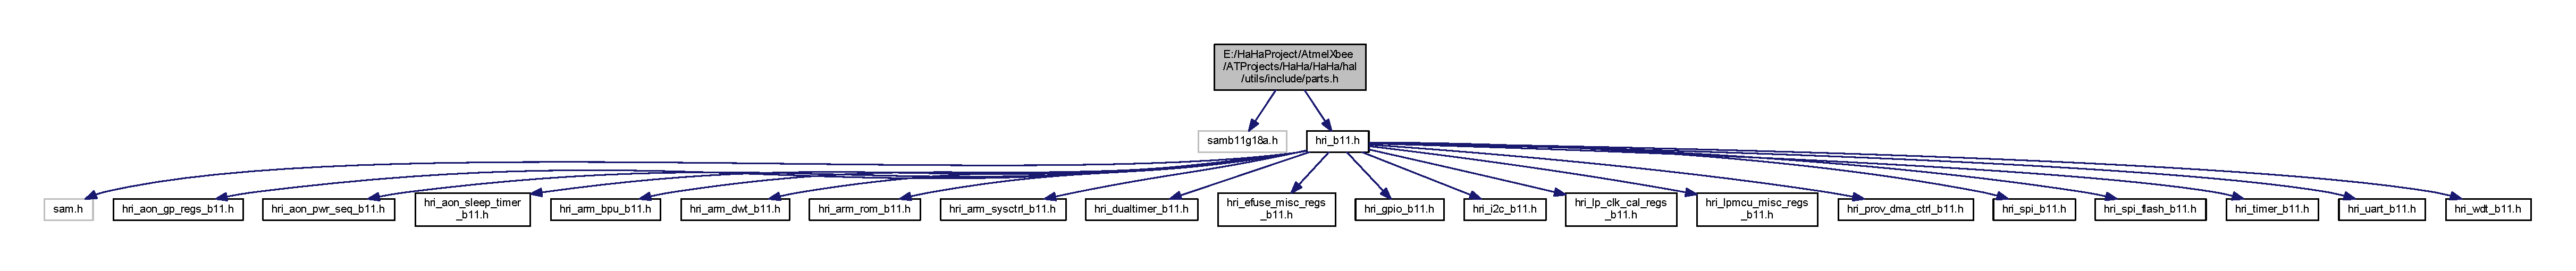
\includegraphics[width=350pt]{parts_8h__incl}
\end{center}
\end{figure}
This graph shows which files directly or indirectly include this file\+:
\nopagebreak
\begin{figure}[H]
\begin{center}
\leavevmode
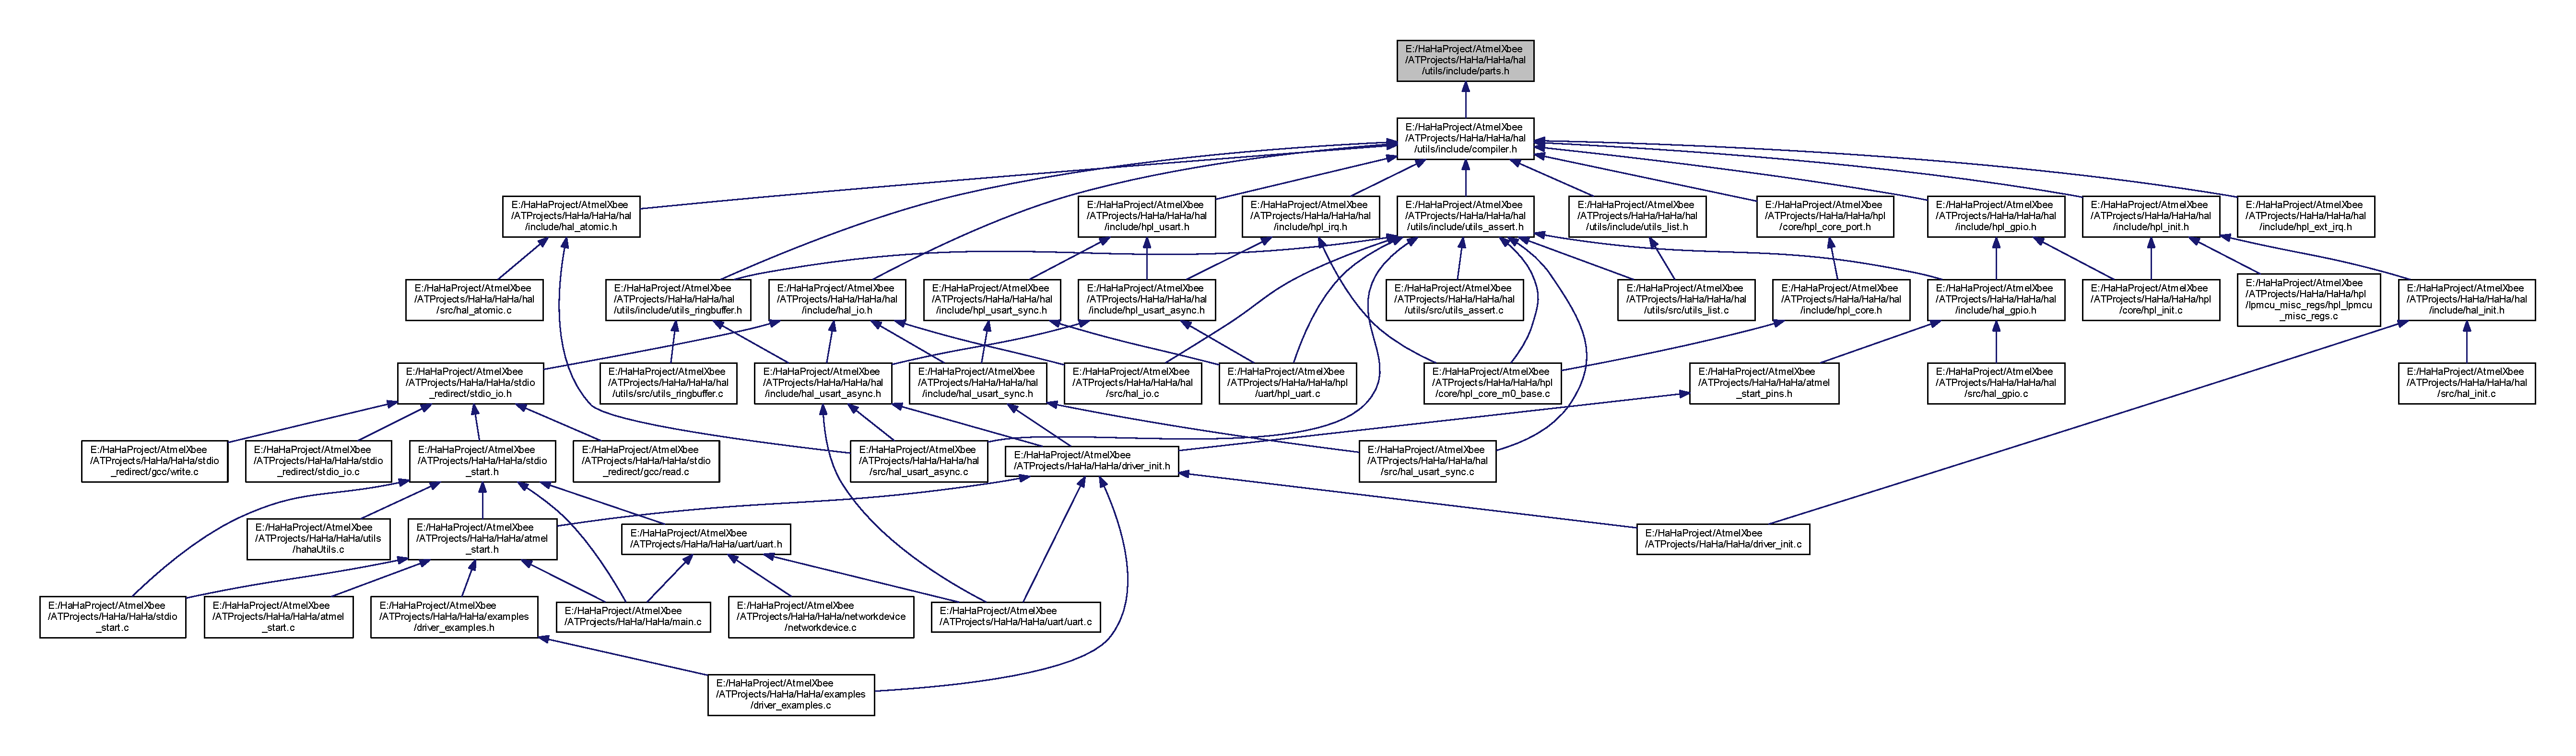
\includegraphics[width=350pt]{parts_8h__dep__incl}
\end{center}
\end{figure}


\subsection{Detailed Description}
Atmel part identification macros. 

Copyright (C) 2015-\/2016 Atmel Corporation. All rights reserved.
\hypertarget{utils_8h}{}\section{E\+:/\+Ha\+Ha\+Project/\+Atmel\+Xbee/\+A\+T\+Projects/\+Ha\+Ha/\+Ha\+Ha/hal/utils/include/utils.h File Reference}
\label{utils_8h}\index{E\+:/\+Ha\+Ha\+Project/\+Atmel\+Xbee/\+A\+T\+Projects/\+Ha\+Ha/\+Ha\+Ha/hal/utils/include/utils.\+h@{E\+:/\+Ha\+Ha\+Project/\+Atmel\+Xbee/\+A\+T\+Projects/\+Ha\+Ha/\+Ha\+Ha/hal/utils/include/utils.\+h}}


Different macros.  


\subsection*{Macros}
\begin{DoxyCompactItemize}
\item 
\#define \hyperlink{group__doc__driver__hal__utils__macro_gae5f8e0a04e100a3953e38a3c7bdbc4f4}{C\+O\+N\+T\+A\+I\+N\+E\+R\+\_\+\+OF}(ptr,  type,  field\+\_\+name)~((type $\ast$)(((uint8\+\_\+t $\ast$)ptr) -\/ offsetof(type, field\+\_\+name)))
\begin{DoxyCompactList}\small\item\em Retrieve pointer to parent structure. \end{DoxyCompactList}\item 
\#define \hyperlink{group__doc__driver__hal__utils__macro_ga25f003de16c08a4888b69f619d70f427}{A\+R\+R\+A\+Y\+\_\+\+S\+I\+ZE}(a)~(sizeof(a) / sizeof((a)\mbox{[}0\mbox{]}))
\begin{DoxyCompactList}\small\item\em Retrieve array size. \end{DoxyCompactList}\item 
\#define \hyperlink{group__doc__driver__hal__utils__macro_ga85a3ab5701281268521f109ed0078668}{C\+O\+M\+P\+I\+L\+E\+R\+\_\+\+P\+R\+A\+G\+MA}(arg)~\+\_\+\+Pragma(\#arg)
\begin{DoxyCompactList}\small\item\em Emit the compiler pragma {\itshape arg}. \end{DoxyCompactList}\item 
\#define \hyperlink{group__doc__driver__hal__utils__macro_gae2c02ff865ca6538b4b1bddbf2a6876c}{C\+O\+M\+P\+I\+L\+E\+R\+\_\+\+P\+A\+C\+K\+\_\+\+S\+ET}(alignment)~\hyperlink{group__doc__driver__hal__utils__macro_ga85a3ab5701281268521f109ed0078668}{C\+O\+M\+P\+I\+L\+E\+R\+\_\+\+P\+R\+A\+G\+MA}(pack(alignment))
\begin{DoxyCompactList}\small\item\em Set maximum alignment for subsequent struct and union definitions to {\itshape alignment}. \end{DoxyCompactList}\item 
\#define \hyperlink{group__doc__driver__hal__utils__macro_ga38d28b622a4bc7b0f3fb2be2ef1e0086}{C\+O\+M\+P\+I\+L\+E\+R\+\_\+\+P\+A\+C\+K\+\_\+\+R\+E\+S\+ET}()~\hyperlink{group__doc__driver__hal__utils__macro_ga85a3ab5701281268521f109ed0078668}{C\+O\+M\+P\+I\+L\+E\+R\+\_\+\+P\+R\+A\+G\+MA}(pack())
\begin{DoxyCompactList}\small\item\em Set default alignment for subsequent struct and union definitions. \end{DoxyCompactList}\item 
\#define {\bfseries L\+E\+\_\+\+B\+Y\+T\+E0}(a)~((uint8\+\_\+t)(a))
\item 
\#define {\bfseries L\+E\+\_\+\+B\+Y\+T\+E1}(a)~((uint8\+\_\+t)((a) $>$$>$ 8))
\item 
\#define {\bfseries L\+E\+\_\+\+B\+Y\+T\+E2}(a)~((uint8\+\_\+t)((a) $>$$>$ 16))
\item 
\#define {\bfseries L\+E\+\_\+\+B\+Y\+T\+E3}(a)~((uint8\+\_\+t)((a) $>$$>$ 24))
\item 
\#define {\bfseries L\+E\+\_\+2\+\_\+\+U16}(p)~((p)\mbox{[}0\mbox{]} + ((p)\mbox{[}1\mbox{]} $<$$<$ 8))
\item 
\#define {\bfseries L\+E\+\_\+2\+\_\+\+U32}(p)~((p)\mbox{[}0\mbox{]} + ((p)\mbox{[}1\mbox{]} $<$$<$ 8) + ((p)\mbox{[}2\mbox{]} $<$$<$ 16) + ((p)\mbox{[}3\mbox{]} $<$$<$ 24))
\item 
\#define \hyperlink{group__doc__driver__hal__utils__macro_gacb24f277663a5c87482fbcdbef5f2bd2}{size\+\_\+of\+\_\+mask}(mask)~(32 -\/ \hyperlink{group__doc__driver__hal__utils__macro_ga004f88903a09b9c23017e697eaf5a845}{clz}(mask) -\/ \hyperlink{group__doc__driver__hal__utils__macro_gab069bfec305db5213465d3b689836404}{ctz}(mask))
\begin{DoxyCompactList}\small\item\em Counts the number of bits in a mask (no more than 32 bits) \end{DoxyCompactList}\item 
\#define \hyperlink{group__doc__driver__hal__utils__macro_ga6e6ec9c159cae4680d073d707063fa0e}{pos\+\_\+of\+\_\+mask}(mask)~\hyperlink{group__doc__driver__hal__utils__macro_gab069bfec305db5213465d3b689836404}{ctz}(mask)
\begin{DoxyCompactList}\small\item\em Retrieve the start position of bits mask (no more than 32 bits) \end{DoxyCompactList}\item 
\#define \hyperlink{group__doc__driver__hal__utils__macro_gab4181d52c8a5083a8f30e3063893f3da}{round\+\_\+up}(a,  b)~(((a)-\/1) / (b) + 1)
\begin{DoxyCompactList}\small\item\em Return division result of a/b and Round up the result to the closest number divisible by \char`\"{}b\char`\"{}. \end{DoxyCompactList}\item 
\#define \hyperlink{group__doc__driver__hal__utils__macro_gabb702d8b501669a23aa0ab3b281b9384}{min}(x,  y)~((x) $>$ (y) ? (y) \+: (x))
\begin{DoxyCompactList}\small\item\em Get the minimal of x and y. \end{DoxyCompactList}\item 
\#define \hyperlink{group__doc__driver__hal__utils__macro_gac39d9cef6a5e030ba8d9e11121054268}{max}(x,  y)~((x) $>$ (y) ? (x) \+: (y))
\begin{DoxyCompactList}\small\item\em Get maximum of x and y. \end{DoxyCompactList}\end{DoxyCompactItemize}
\begin{Indent}\textbf{ Zero-\/\+Bit Counting}\par
{\em Under G\+CC, \+\_\+\+\_\+builtin\+\_\+clz and \+\_\+\+\_\+builtin\+\_\+ctz behave like macros when applied to constant expressions (values known at compile time), so they are more optimized than the use of the corresponding assembly instructions and they can be used as constant expressions e.\+g. to initialize objects having static storage duration, and like the corresponding assembly instructions when applied to non-\/constant expressions (values unknown at compile time), so they are more optimized than an assembly periphrasis. Hence, clz and ctz ensure a possible and optimized behavior for both constant and non-\/constant expressions. }\begin{DoxyCompactItemize}
\item 
\#define \hyperlink{group__doc__driver__hal__utils__macro_ga004f88903a09b9c23017e697eaf5a845}{clz}(u)
\begin{DoxyCompactList}\small\item\em Counts the leading zero bits of the given value considered as a 32-\/bit integer. \end{DoxyCompactList}\item 
\#define \hyperlink{group__doc__driver__hal__utils__macro_gab069bfec305db5213465d3b689836404}{ctz}(u)
\begin{DoxyCompactList}\small\item\em Counts the trailing zero bits of the given value considered as a 32-\/bit integer. \end{DoxyCompactList}\end{DoxyCompactItemize}
\end{Indent}
\subsection*{Typedefs}
\begin{DoxyCompactItemize}
\item 
typedef void($\ast$ \hyperlink{group__doc__driver__hal__utils__macro_gae40b38bc5f5a5bd452bdd59c67d9a9cf}{F\+U\+N\+C\+\_\+\+P\+TR}) (void)
\begin{DoxyCompactList}\small\item\em Set aligned boundary. \end{DoxyCompactList}\end{DoxyCompactItemize}


\subsection{Detailed Description}
Different macros. 

Copyright (C) 2014-\/2016 Atmel Corporation. All rights reserved.
\hypertarget{utils__assert_8h}{}\section{E\+:/\+Ha\+Ha\+Project/\+Atmel\+Xbee/\+A\+T\+Projects/\+Ha\+Ha/\+Ha\+Ha/hal/utils/include/utils\+\_\+assert.h File Reference}
\label{utils__assert_8h}\index{E\+:/\+Ha\+Ha\+Project/\+Atmel\+Xbee/\+A\+T\+Projects/\+Ha\+Ha/\+Ha\+Ha/hal/utils/include/utils\+\_\+assert.\+h@{E\+:/\+Ha\+Ha\+Project/\+Atmel\+Xbee/\+A\+T\+Projects/\+Ha\+Ha/\+Ha\+Ha/hal/utils/include/utils\+\_\+assert.\+h}}


Asserts related functionality.  


{\ttfamily \#include $<$compiler.\+h$>$}\newline
Include dependency graph for utils\+\_\+assert.\+h\+:\nopagebreak
\begin{figure}[H]
\begin{center}
\leavevmode
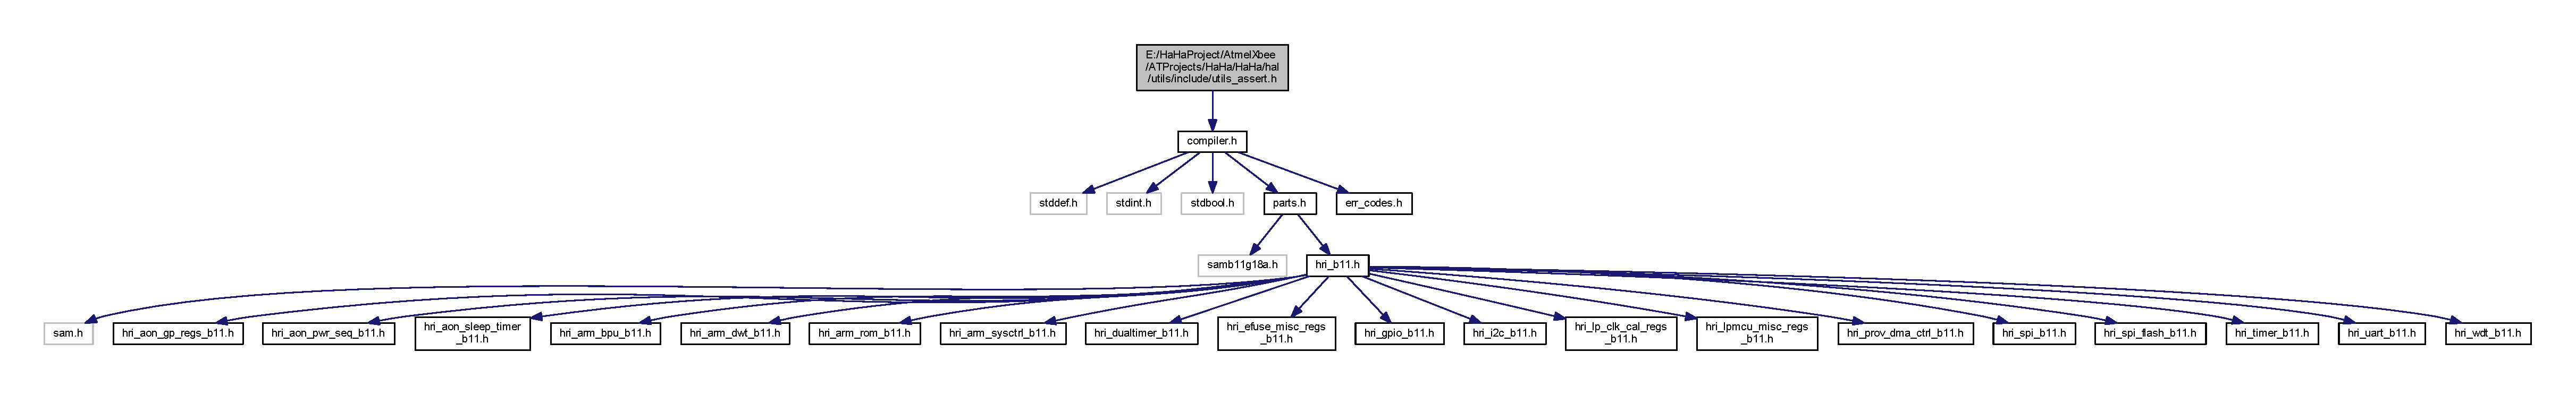
\includegraphics[width=350pt]{utils__assert_8h__incl}
\end{center}
\end{figure}
This graph shows which files directly or indirectly include this file\+:\nopagebreak
\begin{figure}[H]
\begin{center}
\leavevmode
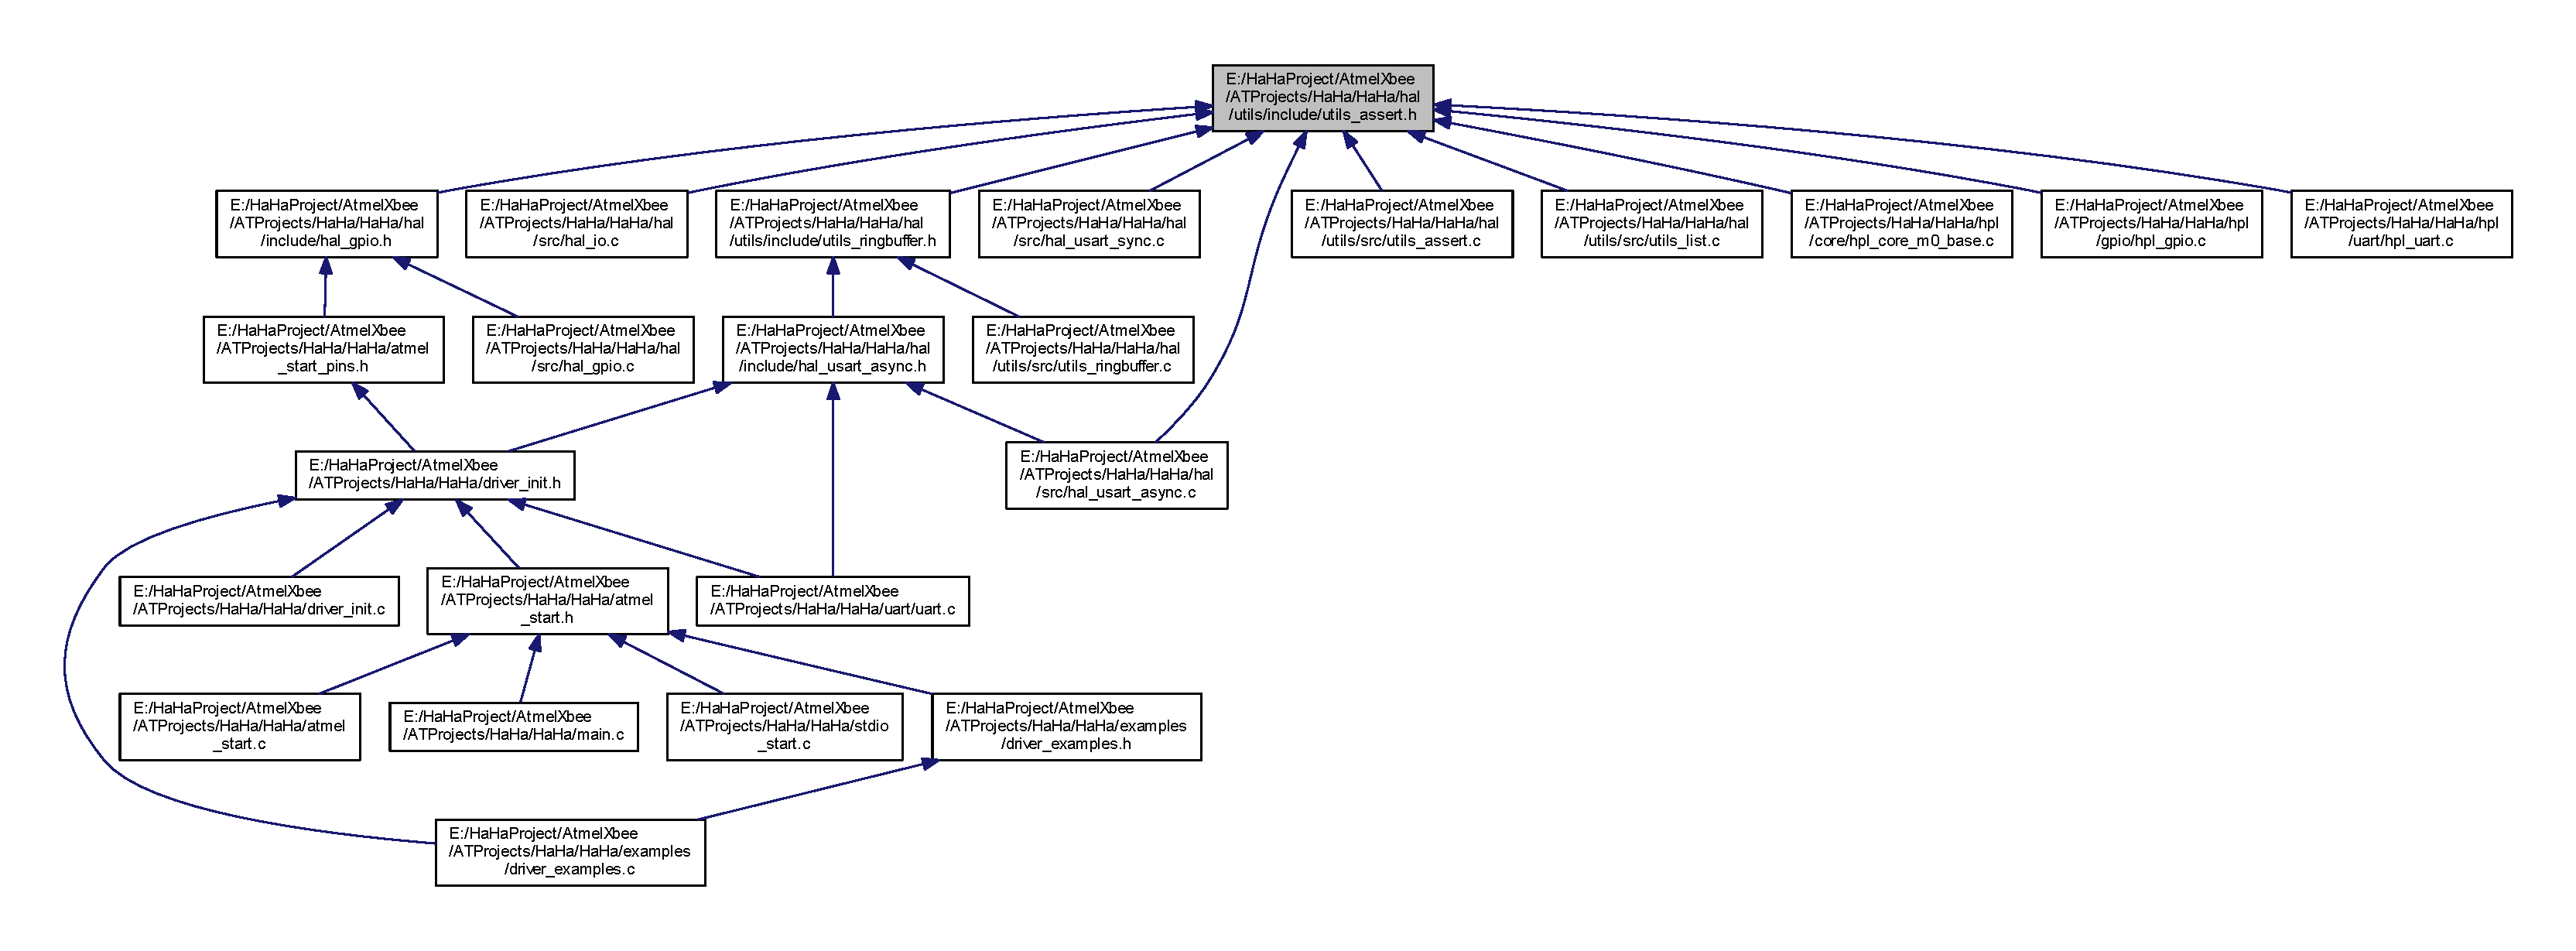
\includegraphics[width=350pt]{utils__assert_8h__dep__incl}
\end{center}
\end{figure}
\subsection*{Macros}
\begin{DoxyCompactItemize}
\item 
\#define \hyperlink{utils__assert_8h_ac22830a985e1daed0c9eadba8c6f606e}{A\+S\+S\+E\+RT}(condition)~\hyperlink{utils__assert_8h_aa8072e041006c526471cd731d62da4ac}{A\+S\+S\+E\+R\+T\+\_\+\+I\+M\+PL}((condition), \+\_\+\+\_\+\+F\+I\+L\+E\+\_\+\+\_\+, \+\_\+\+\_\+\+L\+I\+N\+E\+\_\+\+\_\+)
\begin{DoxyCompactList}\small\item\em Assert macro. \end{DoxyCompactList}\item 
\#define \hyperlink{utils__assert_8h_aa8072e041006c526471cd731d62da4ac}{A\+S\+S\+E\+R\+T\+\_\+\+I\+M\+PL}(condition,  file,  line)~((void)0)
\end{DoxyCompactItemize}
\subsection*{Functions}
\begin{DoxyCompactItemize}
\item 
void \hyperlink{utils__assert_8h_a2b3996392d905d2f6a2f85ad2b173f64}{assert} (const bool condition, const char $\ast$const file, const int line)
\begin{DoxyCompactList}\small\item\em Assert function. \end{DoxyCompactList}\end{DoxyCompactItemize}


\subsection{Detailed Description}
Asserts related functionality. 

Copyright (C) 2014 Atmel Corporation. All rights reserved.

\subsection{Macro Definition Documentation}
\mbox{\Hypertarget{utils__assert_8h_ac22830a985e1daed0c9eadba8c6f606e}\label{utils__assert_8h_ac22830a985e1daed0c9eadba8c6f606e}} 
\index{utils\+\_\+assert.\+h@{utils\+\_\+assert.\+h}!A\+S\+S\+E\+RT@{A\+S\+S\+E\+RT}}
\index{A\+S\+S\+E\+RT@{A\+S\+S\+E\+RT}!utils\+\_\+assert.\+h@{utils\+\_\+assert.\+h}}
\subsubsection{\texorpdfstring{A\+S\+S\+E\+RT}{ASSERT}}
{\footnotesize\ttfamily \#define A\+S\+S\+E\+RT(\begin{DoxyParamCaption}\item[{}]{condition }\end{DoxyParamCaption})~\hyperlink{utils__assert_8h_aa8072e041006c526471cd731d62da4ac}{A\+S\+S\+E\+R\+T\+\_\+\+I\+M\+PL}((condition), \+\_\+\+\_\+\+F\+I\+L\+E\+\_\+\+\_\+, \+\_\+\+\_\+\+L\+I\+N\+E\+\_\+\+\_\+)}



Assert macro. 

This macro is used to throw asserts. It can be mapped to different function based on debug level.


\begin{DoxyParams}[1]{Parameters}
\mbox{\tt in}  & {\em condition} & A condition to be checked; assert is thrown if the given condifition is false \\
\hline
\end{DoxyParams}
\mbox{\Hypertarget{utils__assert_8h_aa8072e041006c526471cd731d62da4ac}\label{utils__assert_8h_aa8072e041006c526471cd731d62da4ac}} 
\index{utils\+\_\+assert.\+h@{utils\+\_\+assert.\+h}!A\+S\+S\+E\+R\+T\+\_\+\+I\+M\+PL@{A\+S\+S\+E\+R\+T\+\_\+\+I\+M\+PL}}
\index{A\+S\+S\+E\+R\+T\+\_\+\+I\+M\+PL@{A\+S\+S\+E\+R\+T\+\_\+\+I\+M\+PL}!utils\+\_\+assert.\+h@{utils\+\_\+assert.\+h}}
\subsubsection{\texorpdfstring{A\+S\+S\+E\+R\+T\+\_\+\+I\+M\+PL}{ASSERT\_IMPL}}
{\footnotesize\ttfamily \#define A\+S\+S\+E\+R\+T\+\_\+\+I\+M\+PL(\begin{DoxyParamCaption}\item[{}]{condition,  }\item[{}]{file,  }\item[{}]{line }\end{DoxyParamCaption})~((void)0)}



\subsection{Function Documentation}
\mbox{\Hypertarget{utils__assert_8h_a2b3996392d905d2f6a2f85ad2b173f64}\label{utils__assert_8h_a2b3996392d905d2f6a2f85ad2b173f64}} 
\index{utils\+\_\+assert.\+h@{utils\+\_\+assert.\+h}!assert@{assert}}
\index{assert@{assert}!utils\+\_\+assert.\+h@{utils\+\_\+assert.\+h}}
\subsubsection{\texorpdfstring{assert()}{assert()}}
{\footnotesize\ttfamily void assert (\begin{DoxyParamCaption}\item[{const bool}]{condition,  }\item[{const char $\ast$const}]{file,  }\item[{const int}]{line }\end{DoxyParamCaption})}



Assert function. 

This function is used to throw asserts.


\begin{DoxyParams}[1]{Parameters}
\mbox{\tt in}  & {\em condition} & A condition to be checked; assert is thrown if the given condition is false \\
\hline
\mbox{\tt in}  & {\em file} & File name \\
\hline
\mbox{\tt in}  & {\em line} & Line number \\
\hline
\end{DoxyParams}

\hypertarget{utils__increment__macro_8h}{}\section{E\+:/\+Ha\+Ha\+Project/\+Atmel\+Xbee/\+A\+T\+Projects/\+Ha\+Ha/\+Ha\+Ha/hal/utils/include/utils\+\_\+increment\+\_\+macro.h File Reference}
\label{utils__increment__macro_8h}\index{E\+:/\+Ha\+Ha\+Project/\+Atmel\+Xbee/\+A\+T\+Projects/\+Ha\+Ha/\+Ha\+Ha/hal/utils/include/utils\+\_\+increment\+\_\+macro.\+h@{E\+:/\+Ha\+Ha\+Project/\+Atmel\+Xbee/\+A\+T\+Projects/\+Ha\+Ha/\+Ha\+Ha/hal/utils/include/utils\+\_\+increment\+\_\+macro.\+h}}


Increment macro.  


This graph shows which files directly or indirectly include this file\+:\nopagebreak
\begin{figure}[H]
\begin{center}
\leavevmode
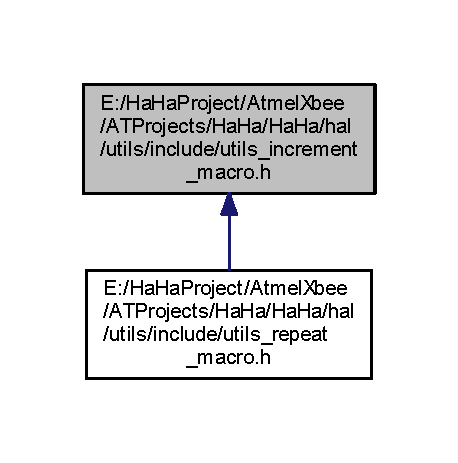
\includegraphics[width=220pt]{utils__increment__macro_8h__dep__incl}
\end{center}
\end{figure}
\subsection*{Macros}
\begin{DoxyCompactItemize}
\item 
\#define \hyperlink{utils__increment__macro_8h_a224df094eda9f558243c300cd524f8e8}{I\+N\+C\+\_\+\+V\+A\+L\+UE}(val)~S\+P\+\_\+\+I\+N\+C\+\_\+\#\#val
\begin{DoxyCompactList}\small\item\em Compile time increment, result value is entire integer literal. \end{DoxyCompactList}\item 
\#define \hyperlink{utils__increment__macro_8h_ae085cf57cd26be0af32831d2bdbd1c93}{S\+P\+\_\+\+I\+N\+C\+\_\+0}~1
\item 
\#define \hyperlink{utils__increment__macro_8h_a9e3737f6a416a955ba7f558ab7be4324}{S\+P\+\_\+\+I\+N\+C\+\_\+1}~2
\item 
\#define \hyperlink{utils__increment__macro_8h_af68ea640810ee8d09e831dc39e3407a7}{S\+P\+\_\+\+I\+N\+C\+\_\+2}~3
\item 
\#define \hyperlink{utils__increment__macro_8h_a8233a6ca7462848989c47d393c87edd7}{S\+P\+\_\+\+I\+N\+C\+\_\+3}~4
\item 
\#define \hyperlink{utils__increment__macro_8h_aa72eceb4231aaa4fd2d21f0dbb10b076}{S\+P\+\_\+\+I\+N\+C\+\_\+4}~5
\item 
\#define \hyperlink{utils__increment__macro_8h_ad2bbbe71a137c9c8b80edf5bc88f475f}{S\+P\+\_\+\+I\+N\+C\+\_\+5}~6
\item 
\#define \hyperlink{utils__increment__macro_8h_a98c5a2f4182cc38919fb418fcb179c2d}{S\+P\+\_\+\+I\+N\+C\+\_\+6}~7
\item 
\#define \hyperlink{utils__increment__macro_8h_a8caba045d68c7024d98793a0b891cb1c}{S\+P\+\_\+\+I\+N\+C\+\_\+7}~8
\item 
\#define \hyperlink{utils__increment__macro_8h_a136011a017617507032ba9e7bf613ddd}{S\+P\+\_\+\+I\+N\+C\+\_\+8}~9
\item 
\#define \hyperlink{utils__increment__macro_8h_ad9f44ddee0e863ddcba783e97e56a690}{S\+P\+\_\+\+I\+N\+C\+\_\+9}~10
\item 
\#define \hyperlink{utils__increment__macro_8h_a3def04c2dfde8bdac5f1ca61fb145864}{S\+P\+\_\+\+I\+N\+C\+\_\+10}~11
\item 
\#define \hyperlink{utils__increment__macro_8h_ab7e1f9b438f41b8ade908e371f87f151}{S\+P\+\_\+\+I\+N\+C\+\_\+11}~12
\item 
\#define \hyperlink{utils__increment__macro_8h_a2071876ac9c3f8ebb4f959dd79ce9654}{S\+P\+\_\+\+I\+N\+C\+\_\+12}~13
\item 
\#define \hyperlink{utils__increment__macro_8h_a677cd11b5c9e45c36b56461596925908}{S\+P\+\_\+\+I\+N\+C\+\_\+13}~14
\item 
\#define \hyperlink{utils__increment__macro_8h_ac9e54faa7726972af6cd2ad623cfe166}{S\+P\+\_\+\+I\+N\+C\+\_\+14}~15
\item 
\#define \hyperlink{utils__increment__macro_8h_ac7a4a7fd10b9fb1d614cf9c6df29279f}{S\+P\+\_\+\+I\+N\+C\+\_\+15}~16
\item 
\#define \hyperlink{utils__increment__macro_8h_a8c3dfb112a80efe6b4db5a4305c43834}{S\+P\+\_\+\+I\+N\+C\+\_\+16}~17
\item 
\#define \hyperlink{utils__increment__macro_8h_a88c9cbc6b1457b2e15d6614eff365d6a}{S\+P\+\_\+\+I\+N\+C\+\_\+17}~18
\item 
\#define \hyperlink{utils__increment__macro_8h_ade9c2af8043afaea0ab21853883867ec}{S\+P\+\_\+\+I\+N\+C\+\_\+18}~19
\item 
\#define \hyperlink{utils__increment__macro_8h_a0fbeb5fa6e804a4c7b24a2cbeae1bfb5}{S\+P\+\_\+\+I\+N\+C\+\_\+19}~20
\item 
\#define \hyperlink{utils__increment__macro_8h_aeaccdb5a1ddb4829c9549a8ddd82dcf3}{S\+P\+\_\+\+I\+N\+C\+\_\+20}~21
\item 
\#define \hyperlink{utils__increment__macro_8h_af8aceaab393826ade7fdf6ac4b55bf9a}{S\+P\+\_\+\+I\+N\+C\+\_\+21}~22
\item 
\#define \hyperlink{utils__increment__macro_8h_a91e97ddaefbb5ceff276eff4582492d4}{S\+P\+\_\+\+I\+N\+C\+\_\+22}~23
\item 
\#define \hyperlink{utils__increment__macro_8h_a8a62064661f6256df3cd0c96e1688273}{S\+P\+\_\+\+I\+N\+C\+\_\+23}~24
\item 
\#define \hyperlink{utils__increment__macro_8h_a3e9630ca48b9ae4cd7a35b77aa11bf65}{S\+P\+\_\+\+I\+N\+C\+\_\+24}~25
\item 
\#define \hyperlink{utils__increment__macro_8h_a6872ae1f36589d0877193b5a56f455ae}{S\+P\+\_\+\+I\+N\+C\+\_\+25}~26
\item 
\#define \hyperlink{utils__increment__macro_8h_a91d859a0551035720c03ced218ed46a6}{S\+P\+\_\+\+I\+N\+C\+\_\+26}~27
\item 
\#define \hyperlink{utils__increment__macro_8h_a2c659053cdc79185f0be28c783957202}{S\+P\+\_\+\+I\+N\+C\+\_\+27}~28
\item 
\#define \hyperlink{utils__increment__macro_8h_ae9fc3fbbc11010d55e2e6be9dd631aa3}{S\+P\+\_\+\+I\+N\+C\+\_\+28}~29
\item 
\#define \hyperlink{utils__increment__macro_8h_ac425dcd3997dd456ca54fdee05655c9e}{S\+P\+\_\+\+I\+N\+C\+\_\+29}~30
\item 
\#define \hyperlink{utils__increment__macro_8h_adda98eebeb056e9e7ab7ec97c6b9a328}{S\+P\+\_\+\+I\+N\+C\+\_\+30}~31
\item 
\#define \hyperlink{utils__increment__macro_8h_a69b5f87b72fa66a38db58b9cd8d471dd}{S\+P\+\_\+\+I\+N\+C\+\_\+31}~32
\item 
\#define \hyperlink{utils__increment__macro_8h_ad778d0656bd8567c3bf9bb50128e29db}{S\+P\+\_\+\+I\+N\+C\+\_\+32}~33
\item 
\#define \hyperlink{utils__increment__macro_8h_aa8dc82c9d60352f17f337d265b76015a}{S\+P\+\_\+\+I\+N\+C\+\_\+33}~34
\item 
\#define \hyperlink{utils__increment__macro_8h_a34908bb77ac01d745e5396c691f048d9}{S\+P\+\_\+\+I\+N\+C\+\_\+34}~35
\item 
\#define \hyperlink{utils__increment__macro_8h_a229f735559157eb606488d3e3dde486a}{S\+P\+\_\+\+I\+N\+C\+\_\+35}~36
\item 
\#define \hyperlink{utils__increment__macro_8h_a23d5583e39a44eddf6b1c60406eac72b}{S\+P\+\_\+\+I\+N\+C\+\_\+36}~37
\item 
\#define \hyperlink{utils__increment__macro_8h_a4bb4ec94dfcfb0b4aa5debb96cb33126}{S\+P\+\_\+\+I\+N\+C\+\_\+37}~38
\item 
\#define \hyperlink{utils__increment__macro_8h_ad8dc8c17c15d585ad0faef4bb5666fad}{S\+P\+\_\+\+I\+N\+C\+\_\+38}~39
\item 
\#define \hyperlink{utils__increment__macro_8h_a5ef86392e79de0ea5021494d38224c9d}{S\+P\+\_\+\+I\+N\+C\+\_\+39}~40
\item 
\#define \hyperlink{utils__increment__macro_8h_a4b6c7beef32e8daa5e6e5a1cb2bb493e}{S\+P\+\_\+\+I\+N\+C\+\_\+40}~41
\item 
\#define \hyperlink{utils__increment__macro_8h_a5bf259f1584ee3dbb542d9a2fc19b988}{S\+P\+\_\+\+I\+N\+C\+\_\+41}~42
\item 
\#define \hyperlink{utils__increment__macro_8h_acea56c4da6b9a5823d1688bc539a1cc8}{S\+P\+\_\+\+I\+N\+C\+\_\+42}~43
\item 
\#define \hyperlink{utils__increment__macro_8h_ac3e81639f94532afe5fcdf0ecce70aa0}{S\+P\+\_\+\+I\+N\+C\+\_\+43}~44
\item 
\#define \hyperlink{utils__increment__macro_8h_ab52352a4ef5008b32a4107b7b538ec8e}{S\+P\+\_\+\+I\+N\+C\+\_\+44}~45
\item 
\#define \hyperlink{utils__increment__macro_8h_ae5be428300357ae7fb4f1012bac0e393}{S\+P\+\_\+\+I\+N\+C\+\_\+45}~46
\item 
\#define \hyperlink{utils__increment__macro_8h_ae6d5472f877b19b7fa41a082c4513ee7}{S\+P\+\_\+\+I\+N\+C\+\_\+46}~47
\item 
\#define \hyperlink{utils__increment__macro_8h_a368e7b3003023f802d13f005d9279ffb}{S\+P\+\_\+\+I\+N\+C\+\_\+47}~48
\item 
\#define \hyperlink{utils__increment__macro_8h_a9acac96a614149a96f2f869f4a5bb67e}{S\+P\+\_\+\+I\+N\+C\+\_\+48}~49
\item 
\#define \hyperlink{utils__increment__macro_8h_a1db0f453c09d89a3954119a8774070a5}{S\+P\+\_\+\+I\+N\+C\+\_\+49}~50
\item 
\#define \hyperlink{utils__increment__macro_8h_a6803e15eb8d26ec9332e2ae56023516b}{S\+P\+\_\+\+I\+N\+C\+\_\+50}~51
\item 
\#define \hyperlink{utils__increment__macro_8h_a514359f8423cfd6dbcf67e87105eff2d}{S\+P\+\_\+\+I\+N\+C\+\_\+51}~52
\item 
\#define \hyperlink{utils__increment__macro_8h_ab97bbde508cdf269eed727d3da41be5c}{S\+P\+\_\+\+I\+N\+C\+\_\+52}~53
\item 
\#define \hyperlink{utils__increment__macro_8h_acd5e76a343b6593aa93debab5869bb61}{S\+P\+\_\+\+I\+N\+C\+\_\+53}~54
\item 
\#define \hyperlink{utils__increment__macro_8h_aa3a14f871bce61dde4968f056b4e3a3e}{S\+P\+\_\+\+I\+N\+C\+\_\+54}~55
\item 
\#define \hyperlink{utils__increment__macro_8h_a48abb4f331686579a8e96bea3c296eae}{S\+P\+\_\+\+I\+N\+C\+\_\+55}~56
\item 
\#define \hyperlink{utils__increment__macro_8h_a47883429fff0a1a36d3633b5d2a3ef07}{S\+P\+\_\+\+I\+N\+C\+\_\+56}~57
\item 
\#define \hyperlink{utils__increment__macro_8h_a1317819835a8e4f9d5593884972b8c75}{S\+P\+\_\+\+I\+N\+C\+\_\+57}~58
\item 
\#define \hyperlink{utils__increment__macro_8h_ad38b7be11eb75a92bf9f075482611662}{S\+P\+\_\+\+I\+N\+C\+\_\+58}~59
\item 
\#define \hyperlink{utils__increment__macro_8h_a4ddbf42527184b083a78521b2f70ad04}{S\+P\+\_\+\+I\+N\+C\+\_\+59}~60
\item 
\#define \hyperlink{utils__increment__macro_8h_a50b008cf2c1d11a139d4d3a87ed00282}{S\+P\+\_\+\+I\+N\+C\+\_\+60}~61
\item 
\#define \hyperlink{utils__increment__macro_8h_a6ba57e805e0ed45d84f533cdf59e22ce}{S\+P\+\_\+\+I\+N\+C\+\_\+61}~62
\item 
\#define \hyperlink{utils__increment__macro_8h_ad26aa57413f6f1c4f97d2050055322ca}{S\+P\+\_\+\+I\+N\+C\+\_\+62}~63
\item 
\#define \hyperlink{utils__increment__macro_8h_a00fb45bd4a82d68b4b89c38660b83c5f}{S\+P\+\_\+\+I\+N\+C\+\_\+63}~64
\item 
\#define \hyperlink{utils__increment__macro_8h_a85aee8b4ad5a846d76f2b6323e120b9d}{S\+P\+\_\+\+I\+N\+C\+\_\+64}~65
\item 
\#define \hyperlink{utils__increment__macro_8h_ae84eb35e1d7d62fad99d9927a3228ba8}{S\+P\+\_\+\+I\+N\+C\+\_\+65}~66
\item 
\#define \hyperlink{utils__increment__macro_8h_a27c4c3cf333b371da7d1abf1e18a8ce8}{S\+P\+\_\+\+I\+N\+C\+\_\+66}~67
\item 
\#define \hyperlink{utils__increment__macro_8h_ab2c43831395cb4b75dea9a95267fbd42}{S\+P\+\_\+\+I\+N\+C\+\_\+67}~68
\item 
\#define \hyperlink{utils__increment__macro_8h_a5d1788fd472fba371f99decfa973f35b}{S\+P\+\_\+\+I\+N\+C\+\_\+68}~69
\item 
\#define \hyperlink{utils__increment__macro_8h_a69ee3715cfdcc21d4e3ce38e181fc12b}{S\+P\+\_\+\+I\+N\+C\+\_\+69}~70
\item 
\#define \hyperlink{utils__increment__macro_8h_aff961a4a9cde2e342d23b9db4c792aab}{S\+P\+\_\+\+I\+N\+C\+\_\+70}~71
\item 
\#define \hyperlink{utils__increment__macro_8h_a69e6370928ddcfdd23c09c4a458ff2d6}{S\+P\+\_\+\+I\+N\+C\+\_\+71}~72
\item 
\#define \hyperlink{utils__increment__macro_8h_a520b4cf6a21a762930ab3b07e9ae8846}{S\+P\+\_\+\+I\+N\+C\+\_\+72}~73
\item 
\#define \hyperlink{utils__increment__macro_8h_ab53b2a87d882864f82394f13699acdbe}{S\+P\+\_\+\+I\+N\+C\+\_\+73}~74
\item 
\#define \hyperlink{utils__increment__macro_8h_a0bfa9b7367234c9ac39da3b95a647803}{S\+P\+\_\+\+I\+N\+C\+\_\+74}~75
\item 
\#define \hyperlink{utils__increment__macro_8h_a9bcbf8f440d1a7817c1520c7dd2bbb66}{S\+P\+\_\+\+I\+N\+C\+\_\+75}~76
\item 
\#define \hyperlink{utils__increment__macro_8h_ae2bf5611cef0bac7ff59b19a4e23196b}{S\+P\+\_\+\+I\+N\+C\+\_\+76}~77
\item 
\#define \hyperlink{utils__increment__macro_8h_a899ce89b1480f4aa9f5bda83dd8584d7}{S\+P\+\_\+\+I\+N\+C\+\_\+77}~78
\item 
\#define \hyperlink{utils__increment__macro_8h_af61d0057d802a1e6daf79493b53679a6}{S\+P\+\_\+\+I\+N\+C\+\_\+78}~79
\item 
\#define \hyperlink{utils__increment__macro_8h_af8fe639001b8b4a4ea42a47ce93a723b}{S\+P\+\_\+\+I\+N\+C\+\_\+79}~80
\item 
\#define \hyperlink{utils__increment__macro_8h_a4ac9690613812aa171171de21984fdc7}{S\+P\+\_\+\+I\+N\+C\+\_\+80}~81
\item 
\#define \hyperlink{utils__increment__macro_8h_a092b6f7121bd224304d1d916e4e74ab7}{S\+P\+\_\+\+I\+N\+C\+\_\+81}~82
\item 
\#define \hyperlink{utils__increment__macro_8h_a60a5414f8f643484d6d0e17e9b84ad6c}{S\+P\+\_\+\+I\+N\+C\+\_\+82}~83
\item 
\#define \hyperlink{utils__increment__macro_8h_ab2f9356d3ad595206957e0975b4b9d8b}{S\+P\+\_\+\+I\+N\+C\+\_\+83}~84
\item 
\#define \hyperlink{utils__increment__macro_8h_a3cdb82cd412cf210090a46236c485d0b}{S\+P\+\_\+\+I\+N\+C\+\_\+84}~85
\item 
\#define \hyperlink{utils__increment__macro_8h_a6e873ddca4dd19c137328b1693771653}{S\+P\+\_\+\+I\+N\+C\+\_\+85}~86
\item 
\#define \hyperlink{utils__increment__macro_8h_ac4902f66993793c5192111ff7db36f6f}{S\+P\+\_\+\+I\+N\+C\+\_\+86}~87
\item 
\#define \hyperlink{utils__increment__macro_8h_a51527fff6d37dcad31f39879b3a86ffe}{S\+P\+\_\+\+I\+N\+C\+\_\+87}~88
\item 
\#define \hyperlink{utils__increment__macro_8h_a75653b51855f1177cbdb61b8f8804be3}{S\+P\+\_\+\+I\+N\+C\+\_\+88}~89
\item 
\#define \hyperlink{utils__increment__macro_8h_a63673e699a4d63524651586937b8aee7}{S\+P\+\_\+\+I\+N\+C\+\_\+89}~90
\item 
\#define \hyperlink{utils__increment__macro_8h_a1078fddc8135b35243301c5f9d464aef}{S\+P\+\_\+\+I\+N\+C\+\_\+90}~91
\item 
\#define \hyperlink{utils__increment__macro_8h_a20d2909d0ca99ba704f9192d82ce01ea}{S\+P\+\_\+\+I\+N\+C\+\_\+91}~92
\item 
\#define \hyperlink{utils__increment__macro_8h_ad301f3e7d88c946b1eec1d51ba281a60}{S\+P\+\_\+\+I\+N\+C\+\_\+92}~93
\item 
\#define \hyperlink{utils__increment__macro_8h_a755b319a045952091f3a3c111795ebdd}{S\+P\+\_\+\+I\+N\+C\+\_\+93}~94
\item 
\#define \hyperlink{utils__increment__macro_8h_a0ba46d871cd95a491e93d03d0a6a48b8}{S\+P\+\_\+\+I\+N\+C\+\_\+94}~95
\item 
\#define \hyperlink{utils__increment__macro_8h_a5da962cfcf17b6ddf610ef3da47f0546}{S\+P\+\_\+\+I\+N\+C\+\_\+95}~96
\item 
\#define \hyperlink{utils__increment__macro_8h_af1f47539dbf8083e02d47fb228d5a257}{S\+P\+\_\+\+I\+N\+C\+\_\+96}~97
\item 
\#define \hyperlink{utils__increment__macro_8h_ae9fe928b56307cdb3e2a33db6c5468e1}{S\+P\+\_\+\+I\+N\+C\+\_\+97}~98
\item 
\#define \hyperlink{utils__increment__macro_8h_a99cd1256b8bbfd8f1a635bee592b4f2f}{S\+P\+\_\+\+I\+N\+C\+\_\+98}~99
\item 
\#define \hyperlink{utils__increment__macro_8h_abbaa68a3b9c9d1a71b968a5c01d1a2aa}{S\+P\+\_\+\+I\+N\+C\+\_\+99}~100
\item 
\#define \hyperlink{utils__increment__macro_8h_aae56fc7c0a8107a608b4ff37afbc7f19}{S\+P\+\_\+\+I\+N\+C\+\_\+100}~101
\item 
\#define \hyperlink{utils__increment__macro_8h_a47982fbb78f8f86aad9ddbba379628ae}{S\+P\+\_\+\+I\+N\+C\+\_\+101}~102
\item 
\#define \hyperlink{utils__increment__macro_8h_ab529b3ce55bc4e3c0a0f553ffe0c8978}{S\+P\+\_\+\+I\+N\+C\+\_\+102}~103
\item 
\#define \hyperlink{utils__increment__macro_8h_ab7b7bf0bbb04fe4a5df4e1c5c9e593c0}{S\+P\+\_\+\+I\+N\+C\+\_\+103}~104
\item 
\#define \hyperlink{utils__increment__macro_8h_ab726e368036b112f04fc131c15676fa2}{S\+P\+\_\+\+I\+N\+C\+\_\+104}~105
\item 
\#define \hyperlink{utils__increment__macro_8h_ad067e33d190b9e4e3ad7ca0303968899}{S\+P\+\_\+\+I\+N\+C\+\_\+105}~106
\item 
\#define \hyperlink{utils__increment__macro_8h_a28f86b2a5cd08b4d8e97066de4353e20}{S\+P\+\_\+\+I\+N\+C\+\_\+106}~107
\item 
\#define \hyperlink{utils__increment__macro_8h_a25bca55238e7f4fc450cc70d7cae3289}{S\+P\+\_\+\+I\+N\+C\+\_\+107}~108
\item 
\#define \hyperlink{utils__increment__macro_8h_af1a50e59de2b2e4ee8dbdf95d8066d86}{S\+P\+\_\+\+I\+N\+C\+\_\+108}~109
\item 
\#define \hyperlink{utils__increment__macro_8h_a214678414db057953e337c292b5a1ab3}{S\+P\+\_\+\+I\+N\+C\+\_\+109}~110
\item 
\#define \hyperlink{utils__increment__macro_8h_ad301f8aec0052444826e366e66cddab7}{S\+P\+\_\+\+I\+N\+C\+\_\+110}~111
\item 
\#define \hyperlink{utils__increment__macro_8h_a3b9cfdf4f75efb21db11ecc08c49af8c}{S\+P\+\_\+\+I\+N\+C\+\_\+111}~112
\item 
\#define \hyperlink{utils__increment__macro_8h_a5e630b5ad5b3007a56a030c99f99b168}{S\+P\+\_\+\+I\+N\+C\+\_\+112}~113
\item 
\#define \hyperlink{utils__increment__macro_8h_a383d1b87fa406466a512fccda3242229}{S\+P\+\_\+\+I\+N\+C\+\_\+113}~114
\item 
\#define \hyperlink{utils__increment__macro_8h_ad3fff1f1642423381867c16d487df9ef}{S\+P\+\_\+\+I\+N\+C\+\_\+114}~115
\item 
\#define \hyperlink{utils__increment__macro_8h_a06f7e4ee2e175d8c551103b1bf8a4bb0}{S\+P\+\_\+\+I\+N\+C\+\_\+115}~116
\item 
\#define \hyperlink{utils__increment__macro_8h_a887d5221533cbbb6b81750840686dc0a}{S\+P\+\_\+\+I\+N\+C\+\_\+116}~117
\item 
\#define \hyperlink{utils__increment__macro_8h_a6f0cea3709d9f76de9d94c131d8f40e7}{S\+P\+\_\+\+I\+N\+C\+\_\+117}~118
\item 
\#define \hyperlink{utils__increment__macro_8h_a1303c6b2034a9691288c76d10d8f8783}{S\+P\+\_\+\+I\+N\+C\+\_\+118}~119
\item 
\#define \hyperlink{utils__increment__macro_8h_a6efc2c6983cc2cdc68b413c21bb7c96b}{S\+P\+\_\+\+I\+N\+C\+\_\+119}~120
\item 
\#define \hyperlink{utils__increment__macro_8h_aa234c4e94d92aff69ac4a8d56f799949}{S\+P\+\_\+\+I\+N\+C\+\_\+120}~121
\item 
\#define \hyperlink{utils__increment__macro_8h_ad6b2268b303a86e208d287660e6a5bf7}{S\+P\+\_\+\+I\+N\+C\+\_\+121}~122
\item 
\#define \hyperlink{utils__increment__macro_8h_a6ac46890c5533d147451b05a50c42ee3}{S\+P\+\_\+\+I\+N\+C\+\_\+122}~123
\item 
\#define \hyperlink{utils__increment__macro_8h_a2b0e3cc3edf986d7d699f7527c3dbc5c}{S\+P\+\_\+\+I\+N\+C\+\_\+123}~124
\item 
\#define \hyperlink{utils__increment__macro_8h_a2ed39f2576a83ec29c46b814cf94e19f}{S\+P\+\_\+\+I\+N\+C\+\_\+124}~125
\item 
\#define \hyperlink{utils__increment__macro_8h_a35fba751878c39dfd7199ce6497fe8a0}{S\+P\+\_\+\+I\+N\+C\+\_\+125}~126
\item 
\#define \hyperlink{utils__increment__macro_8h_aa2ad15fc0ef1b77ef87acb5af65b429f}{S\+P\+\_\+\+I\+N\+C\+\_\+126}~127
\item 
\#define \hyperlink{utils__increment__macro_8h_ac2da54d6d26c47614fbf5bca8e8041c4}{S\+P\+\_\+\+I\+N\+C\+\_\+127}~128
\item 
\#define \hyperlink{utils__increment__macro_8h_a61f70f8a80cfe058644f0fc42ca4fd5e}{S\+P\+\_\+\+I\+N\+C\+\_\+128}~129
\item 
\#define \hyperlink{utils__increment__macro_8h_ad784d3de6e6a06c624bed55e9ba2d1b6}{S\+P\+\_\+\+I\+N\+C\+\_\+129}~130
\item 
\#define \hyperlink{utils__increment__macro_8h_a16ed690f006fc68b39c14e37a9fdbdd8}{S\+P\+\_\+\+I\+N\+C\+\_\+130}~131
\item 
\#define \hyperlink{utils__increment__macro_8h_a26fabd6c73f9d1c67db22efc4d6065f2}{S\+P\+\_\+\+I\+N\+C\+\_\+131}~132
\item 
\#define \hyperlink{utils__increment__macro_8h_a1ec0208f63db8a90982bb1cd95371acf}{S\+P\+\_\+\+I\+N\+C\+\_\+132}~133
\item 
\#define \hyperlink{utils__increment__macro_8h_a059c5822e7df4f038a9487970c7f3272}{S\+P\+\_\+\+I\+N\+C\+\_\+133}~134
\item 
\#define \hyperlink{utils__increment__macro_8h_a7352a9310666a825efd4766a1dfdb80b}{S\+P\+\_\+\+I\+N\+C\+\_\+134}~135
\item 
\#define \hyperlink{utils__increment__macro_8h_a1383bc6f3aeccdcb4a1c519cd37d87f2}{S\+P\+\_\+\+I\+N\+C\+\_\+135}~136
\item 
\#define \hyperlink{utils__increment__macro_8h_a438d2a75e70bc4d79f63d768d1a809c4}{S\+P\+\_\+\+I\+N\+C\+\_\+136}~137
\item 
\#define \hyperlink{utils__increment__macro_8h_a280c43b99d6da5c4d362a747546ff689}{S\+P\+\_\+\+I\+N\+C\+\_\+137}~138
\item 
\#define \hyperlink{utils__increment__macro_8h_a95df26d9236659284a9ac2d3f0b12446}{S\+P\+\_\+\+I\+N\+C\+\_\+138}~139
\item 
\#define \hyperlink{utils__increment__macro_8h_a3c313d1cb8f5e64fdbb6304a1647a5ec}{S\+P\+\_\+\+I\+N\+C\+\_\+139}~140
\item 
\#define \hyperlink{utils__increment__macro_8h_afa8f14600237d5e36507a875fff77d3b}{S\+P\+\_\+\+I\+N\+C\+\_\+140}~141
\item 
\#define \hyperlink{utils__increment__macro_8h_a4a392626280e71dd3fe7ae7e0c01978f}{S\+P\+\_\+\+I\+N\+C\+\_\+141}~142
\item 
\#define \hyperlink{utils__increment__macro_8h_acde5ae4d916efa73efaf04817816b7d1}{S\+P\+\_\+\+I\+N\+C\+\_\+142}~143
\item 
\#define \hyperlink{utils__increment__macro_8h_a30ddd7885feb0b5c245a0527a643fb4d}{S\+P\+\_\+\+I\+N\+C\+\_\+143}~144
\item 
\#define \hyperlink{utils__increment__macro_8h_a7913c41733df888b886e731bc97ece2e}{S\+P\+\_\+\+I\+N\+C\+\_\+144}~145
\item 
\#define \hyperlink{utils__increment__macro_8h_af601e56b8b175df072ad5a088fc450b7}{S\+P\+\_\+\+I\+N\+C\+\_\+145}~146
\item 
\#define \hyperlink{utils__increment__macro_8h_aaa39d5a1266aac2b7dd2f0bf4c082886}{S\+P\+\_\+\+I\+N\+C\+\_\+146}~147
\item 
\#define \hyperlink{utils__increment__macro_8h_a87a33f60efdc40da2737619500b6fd08}{S\+P\+\_\+\+I\+N\+C\+\_\+147}~148
\item 
\#define \hyperlink{utils__increment__macro_8h_a34a93c3f6d565dfeab9ffbf803511e9a}{S\+P\+\_\+\+I\+N\+C\+\_\+148}~149
\item 
\#define \hyperlink{utils__increment__macro_8h_a1fccf57d0aea8328404c8443e777c85e}{S\+P\+\_\+\+I\+N\+C\+\_\+149}~150
\item 
\#define \hyperlink{utils__increment__macro_8h_a4fab06715145d0766b9e527f5d50ff8f}{S\+P\+\_\+\+I\+N\+C\+\_\+150}~151
\item 
\#define \hyperlink{utils__increment__macro_8h_a2074b0cb8c206c646c23688348ee4f6c}{S\+P\+\_\+\+I\+N\+C\+\_\+151}~152
\item 
\#define \hyperlink{utils__increment__macro_8h_afd19e09d47ee4c0bb53cf1864bd1f8cb}{S\+P\+\_\+\+I\+N\+C\+\_\+152}~153
\item 
\#define \hyperlink{utils__increment__macro_8h_a1b014c80bbb9ba449d475b040052d4cb}{S\+P\+\_\+\+I\+N\+C\+\_\+153}~154
\item 
\#define \hyperlink{utils__increment__macro_8h_a8afd88cb18038686dc6043e0d51739cc}{S\+P\+\_\+\+I\+N\+C\+\_\+154}~155
\item 
\#define \hyperlink{utils__increment__macro_8h_a356a5b5a1e0098d24365f91eee400079}{S\+P\+\_\+\+I\+N\+C\+\_\+155}~156
\item 
\#define \hyperlink{utils__increment__macro_8h_a8f5de5dec3015bf95967ef326addea34}{S\+P\+\_\+\+I\+N\+C\+\_\+156}~157
\item 
\#define \hyperlink{utils__increment__macro_8h_a08c7e4792dbdc1c55c41c945b4d2f999}{S\+P\+\_\+\+I\+N\+C\+\_\+157}~158
\item 
\#define \hyperlink{utils__increment__macro_8h_a4c1371a91e8dbb71bf3f72258fdf2c53}{S\+P\+\_\+\+I\+N\+C\+\_\+158}~159
\item 
\#define \hyperlink{utils__increment__macro_8h_ad210be7fa3d4ae7ee82b00dc722e3348}{S\+P\+\_\+\+I\+N\+C\+\_\+159}~160
\item 
\#define \hyperlink{utils__increment__macro_8h_ab2093623cf2416f864a3289575aa2f18}{S\+P\+\_\+\+I\+N\+C\+\_\+160}~161
\item 
\#define \hyperlink{utils__increment__macro_8h_a702ac744d6cd6eae842d226c49fb1b51}{S\+P\+\_\+\+I\+N\+C\+\_\+161}~162
\item 
\#define \hyperlink{utils__increment__macro_8h_afb6c5b07f97c77265bc1394758d5d639}{S\+P\+\_\+\+I\+N\+C\+\_\+162}~163
\item 
\#define \hyperlink{utils__increment__macro_8h_aeb4a93a0b44b7fb9644a1055a4d28cc0}{S\+P\+\_\+\+I\+N\+C\+\_\+163}~164
\item 
\#define \hyperlink{utils__increment__macro_8h_a6dba02726b169a853baecf905b0d8ad2}{S\+P\+\_\+\+I\+N\+C\+\_\+164}~165
\item 
\#define \hyperlink{utils__increment__macro_8h_a95b0f62d0a1a1693cd75aa8a9ad176eb}{S\+P\+\_\+\+I\+N\+C\+\_\+165}~166
\item 
\#define \hyperlink{utils__increment__macro_8h_a8b30ad0a6920dbc1137d16059f3cc447}{S\+P\+\_\+\+I\+N\+C\+\_\+166}~167
\item 
\#define \hyperlink{utils__increment__macro_8h_a91399a47ca4e9c9bbdae63dbc6496cf5}{S\+P\+\_\+\+I\+N\+C\+\_\+167}~168
\item 
\#define \hyperlink{utils__increment__macro_8h_a1bb2ac8cc0c818e9d23ddbbc8da7463f}{S\+P\+\_\+\+I\+N\+C\+\_\+168}~169
\item 
\#define \hyperlink{utils__increment__macro_8h_af9f2d81cc87c8dafd2bdc20b7c17e09e}{S\+P\+\_\+\+I\+N\+C\+\_\+169}~170
\item 
\#define \hyperlink{utils__increment__macro_8h_a1d664cfde5e1699eebee7c4ef4254f77}{S\+P\+\_\+\+I\+N\+C\+\_\+170}~171
\item 
\#define \hyperlink{utils__increment__macro_8h_a190cd051ed40be1b2b18c6232137ee09}{S\+P\+\_\+\+I\+N\+C\+\_\+171}~172
\item 
\#define \hyperlink{utils__increment__macro_8h_ae1902f9d1899baa7707ce34e6d8a97c2}{S\+P\+\_\+\+I\+N\+C\+\_\+172}~173
\item 
\#define \hyperlink{utils__increment__macro_8h_a711ec223cb14e95fd0edefeada915843}{S\+P\+\_\+\+I\+N\+C\+\_\+173}~174
\item 
\#define \hyperlink{utils__increment__macro_8h_ae8d43116b062b832f994be9e05a42382}{S\+P\+\_\+\+I\+N\+C\+\_\+174}~175
\item 
\#define \hyperlink{utils__increment__macro_8h_a0df3d7db7c74edc5c72a3fccea824b03}{S\+P\+\_\+\+I\+N\+C\+\_\+175}~176
\item 
\#define \hyperlink{utils__increment__macro_8h_a30e9d4ef04037adfc316740b0457570c}{S\+P\+\_\+\+I\+N\+C\+\_\+176}~177
\item 
\#define \hyperlink{utils__increment__macro_8h_a70bcb91684ae7e4118e78e370e85b39e}{S\+P\+\_\+\+I\+N\+C\+\_\+177}~178
\item 
\#define \hyperlink{utils__increment__macro_8h_a12e8bbed671a241261a8cb4519503ac4}{S\+P\+\_\+\+I\+N\+C\+\_\+178}~179
\item 
\#define \hyperlink{utils__increment__macro_8h_a022504c243ce59a9cd1a89995a7316de}{S\+P\+\_\+\+I\+N\+C\+\_\+179}~180
\item 
\#define \hyperlink{utils__increment__macro_8h_af125bd4bc8611f5919cfddd149e326a7}{S\+P\+\_\+\+I\+N\+C\+\_\+180}~181
\item 
\#define \hyperlink{utils__increment__macro_8h_a54ce6a303c82837be84a824bd738c5f6}{S\+P\+\_\+\+I\+N\+C\+\_\+181}~182
\item 
\#define \hyperlink{utils__increment__macro_8h_a22d327a4066ef2bf393df8dc43db3f46}{S\+P\+\_\+\+I\+N\+C\+\_\+182}~183
\item 
\#define \hyperlink{utils__increment__macro_8h_a003c7d3bad42fa17813f30af040006e1}{S\+P\+\_\+\+I\+N\+C\+\_\+183}~184
\item 
\#define \hyperlink{utils__increment__macro_8h_a5d1690b2c32934582246218d8ddf6354}{S\+P\+\_\+\+I\+N\+C\+\_\+184}~185
\item 
\#define \hyperlink{utils__increment__macro_8h_ae8b8ea2f9a5bbcaaa0b3cd63c2908cfb}{S\+P\+\_\+\+I\+N\+C\+\_\+185}~186
\item 
\#define \hyperlink{utils__increment__macro_8h_ae143ea58f4a3292d0a87be7f2377fabc}{S\+P\+\_\+\+I\+N\+C\+\_\+186}~187
\item 
\#define \hyperlink{utils__increment__macro_8h_ae70c60a5ba7e58b8a848188797bdb702}{S\+P\+\_\+\+I\+N\+C\+\_\+187}~188
\item 
\#define \hyperlink{utils__increment__macro_8h_a3a84cac65a2d838857b399eb7afa2339}{S\+P\+\_\+\+I\+N\+C\+\_\+188}~189
\item 
\#define \hyperlink{utils__increment__macro_8h_a175bc15a328a160208cbae7519050afb}{S\+P\+\_\+\+I\+N\+C\+\_\+189}~190
\item 
\#define \hyperlink{utils__increment__macro_8h_a7f0fe66eed0f8d59e0120d84c4a71a4c}{S\+P\+\_\+\+I\+N\+C\+\_\+190}~191
\item 
\#define \hyperlink{utils__increment__macro_8h_ae6820bbda168849a217a55a759fc8dce}{S\+P\+\_\+\+I\+N\+C\+\_\+191}~192
\item 
\#define \hyperlink{utils__increment__macro_8h_a26b7c5048a9b5bc0537454e76c3e771c}{S\+P\+\_\+\+I\+N\+C\+\_\+192}~193
\item 
\#define \hyperlink{utils__increment__macro_8h_a793146158dd7944a43bd96ee12236b92}{S\+P\+\_\+\+I\+N\+C\+\_\+193}~194
\item 
\#define \hyperlink{utils__increment__macro_8h_a788874e51814f02b16890571c9dd723b}{S\+P\+\_\+\+I\+N\+C\+\_\+194}~195
\item 
\#define \hyperlink{utils__increment__macro_8h_a588e3e1140a9ffb8b1c080be2edbdcf4}{S\+P\+\_\+\+I\+N\+C\+\_\+195}~196
\item 
\#define \hyperlink{utils__increment__macro_8h_a531fa52c6cf5bec637a579d51114010e}{S\+P\+\_\+\+I\+N\+C\+\_\+196}~197
\item 
\#define \hyperlink{utils__increment__macro_8h_aa94892ef83ae50542aec4b2c47baa836}{S\+P\+\_\+\+I\+N\+C\+\_\+197}~198
\item 
\#define \hyperlink{utils__increment__macro_8h_ad67d34247c409efc683fdaba82eb1b4c}{S\+P\+\_\+\+I\+N\+C\+\_\+198}~199
\item 
\#define \hyperlink{utils__increment__macro_8h_aea3b58fe55396c0ce8d9c01c1bfe90d0}{S\+P\+\_\+\+I\+N\+C\+\_\+199}~200
\item 
\#define \hyperlink{utils__increment__macro_8h_a243b021630fbba43f9fb5c2947073548}{S\+P\+\_\+\+I\+N\+C\+\_\+200}~201
\item 
\#define \hyperlink{utils__increment__macro_8h_a7355bf36073d739ed751facb6effbb29}{S\+P\+\_\+\+I\+N\+C\+\_\+201}~202
\item 
\#define \hyperlink{utils__increment__macro_8h_a91defe6de3a9f4b64e9455b61e595583}{S\+P\+\_\+\+I\+N\+C\+\_\+202}~203
\item 
\#define \hyperlink{utils__increment__macro_8h_a955455e48ae02360e2ad611f1097842e}{S\+P\+\_\+\+I\+N\+C\+\_\+203}~204
\item 
\#define \hyperlink{utils__increment__macro_8h_a77454b3186893860998b8034361c21a5}{S\+P\+\_\+\+I\+N\+C\+\_\+204}~205
\item 
\#define \hyperlink{utils__increment__macro_8h_aa2b3ed347ce309630ab62bdb171bc2d9}{S\+P\+\_\+\+I\+N\+C\+\_\+205}~206
\item 
\#define \hyperlink{utils__increment__macro_8h_a8b1370df03c2a33cfda7db5c1df12f85}{S\+P\+\_\+\+I\+N\+C\+\_\+206}~207
\item 
\#define \hyperlink{utils__increment__macro_8h_aee9e6124ffc08465e0e3498b7e3ed334}{S\+P\+\_\+\+I\+N\+C\+\_\+207}~208
\item 
\#define \hyperlink{utils__increment__macro_8h_a70b71728438c8eb99dac3e99b9eed585}{S\+P\+\_\+\+I\+N\+C\+\_\+208}~209
\item 
\#define \hyperlink{utils__increment__macro_8h_a1fbc20104f0b49f0a990e5ef38747ba0}{S\+P\+\_\+\+I\+N\+C\+\_\+209}~210
\item 
\#define \hyperlink{utils__increment__macro_8h_a29c2c3c9809acb024d0dae6752946cd1}{S\+P\+\_\+\+I\+N\+C\+\_\+210}~211
\item 
\#define \hyperlink{utils__increment__macro_8h_af4e63499ab125d3ee8184152dcd0e976}{S\+P\+\_\+\+I\+N\+C\+\_\+211}~212
\item 
\#define \hyperlink{utils__increment__macro_8h_a2362eb2cb1874eff9a5c539b9f0ffe56}{S\+P\+\_\+\+I\+N\+C\+\_\+212}~213
\item 
\#define \hyperlink{utils__increment__macro_8h_aabf45f08ed3d77bdad05ec23982fded7}{S\+P\+\_\+\+I\+N\+C\+\_\+213}~214
\item 
\#define \hyperlink{utils__increment__macro_8h_aa532a21dd0c5fcf0ca3dc85466fa96d7}{S\+P\+\_\+\+I\+N\+C\+\_\+214}~215
\item 
\#define \hyperlink{utils__increment__macro_8h_aecf99036230ed0eeaa7cd19ac353409e}{S\+P\+\_\+\+I\+N\+C\+\_\+215}~216
\item 
\#define \hyperlink{utils__increment__macro_8h_a3e1c96870461a0bf0bb7f1f87f3fab1d}{S\+P\+\_\+\+I\+N\+C\+\_\+216}~217
\item 
\#define \hyperlink{utils__increment__macro_8h_a3cb4e9aa1a7d7115d97ae1b11cc13afd}{S\+P\+\_\+\+I\+N\+C\+\_\+217}~218
\item 
\#define \hyperlink{utils__increment__macro_8h_a8721182198b7e0f0facad4ea86efe022}{S\+P\+\_\+\+I\+N\+C\+\_\+218}~219
\item 
\#define \hyperlink{utils__increment__macro_8h_ad7159088a239fae28c39a8210b6c275c}{S\+P\+\_\+\+I\+N\+C\+\_\+219}~220
\item 
\#define \hyperlink{utils__increment__macro_8h_a7f7c0c5b4946245ff926ee10751c0096}{S\+P\+\_\+\+I\+N\+C\+\_\+220}~221
\item 
\#define \hyperlink{utils__increment__macro_8h_a64b4247df99d33ddc26cd962cd7f6cab}{S\+P\+\_\+\+I\+N\+C\+\_\+221}~222
\item 
\#define \hyperlink{utils__increment__macro_8h_a1dbdf712c74068be88f3a1ba4d588a11}{S\+P\+\_\+\+I\+N\+C\+\_\+222}~223
\item 
\#define \hyperlink{utils__increment__macro_8h_ab81f73aa1998d955a0cd5f1ffe02f3f3}{S\+P\+\_\+\+I\+N\+C\+\_\+223}~224
\item 
\#define \hyperlink{utils__increment__macro_8h_a944b5358516d1f4a8db5a1170ca6d8b8}{S\+P\+\_\+\+I\+N\+C\+\_\+224}~225
\item 
\#define \hyperlink{utils__increment__macro_8h_a19fd41e813c351d24ac29de7050face0}{S\+P\+\_\+\+I\+N\+C\+\_\+225}~226
\item 
\#define \hyperlink{utils__increment__macro_8h_ad26027b53f9d6492e2442411962a4cd9}{S\+P\+\_\+\+I\+N\+C\+\_\+226}~227
\item 
\#define \hyperlink{utils__increment__macro_8h_a52d44683d74ee92ac5d8b0aba58636a6}{S\+P\+\_\+\+I\+N\+C\+\_\+227}~228
\item 
\#define \hyperlink{utils__increment__macro_8h_a2c5101ea47893705f3a82792e6fdb2d2}{S\+P\+\_\+\+I\+N\+C\+\_\+228}~229
\item 
\#define \hyperlink{utils__increment__macro_8h_a9fd8351bb840c1e61e0039c85d2026cb}{S\+P\+\_\+\+I\+N\+C\+\_\+229}~230
\item 
\#define \hyperlink{utils__increment__macro_8h_a001160a7e279a6f5b69c7ee1c06034fc}{S\+P\+\_\+\+I\+N\+C\+\_\+230}~231
\item 
\#define \hyperlink{utils__increment__macro_8h_aac76f25f8ffc9e91202452209c70ac5e}{S\+P\+\_\+\+I\+N\+C\+\_\+231}~232
\item 
\#define \hyperlink{utils__increment__macro_8h_afdbbeb6b03570cd2ebb3c2151ebda945}{S\+P\+\_\+\+I\+N\+C\+\_\+232}~233
\item 
\#define \hyperlink{utils__increment__macro_8h_a9d6e1c56395310f207216f01d795656e}{S\+P\+\_\+\+I\+N\+C\+\_\+233}~234
\item 
\#define \hyperlink{utils__increment__macro_8h_ac6ac05fc8d6fb20da2065cf79f955d4f}{S\+P\+\_\+\+I\+N\+C\+\_\+234}~235
\item 
\#define \hyperlink{utils__increment__macro_8h_a17a06d72978134fa3ab0b2cf5b05af12}{S\+P\+\_\+\+I\+N\+C\+\_\+235}~236
\item 
\#define \hyperlink{utils__increment__macro_8h_a4e0aff93a044c279c76fae9f324055de}{S\+P\+\_\+\+I\+N\+C\+\_\+236}~237
\item 
\#define \hyperlink{utils__increment__macro_8h_ad395afcc1aa0a1ba63a5f5f731ac3294}{S\+P\+\_\+\+I\+N\+C\+\_\+237}~238
\item 
\#define \hyperlink{utils__increment__macro_8h_a91ee3eba99a769792d60f977ab3aeca5}{S\+P\+\_\+\+I\+N\+C\+\_\+238}~239
\item 
\#define \hyperlink{utils__increment__macro_8h_a38b7f6e9dda3436faa160eea77845937}{S\+P\+\_\+\+I\+N\+C\+\_\+239}~240
\item 
\#define \hyperlink{utils__increment__macro_8h_aa2099d9a4f6006acdfd26f154ff6c7a7}{S\+P\+\_\+\+I\+N\+C\+\_\+240}~241
\item 
\#define \hyperlink{utils__increment__macro_8h_a7fb396c5c0aea616d4a998b8144aff31}{S\+P\+\_\+\+I\+N\+C\+\_\+241}~242
\item 
\#define \hyperlink{utils__increment__macro_8h_ac457e3133b4aff429571acf3bff13365}{S\+P\+\_\+\+I\+N\+C\+\_\+242}~243
\item 
\#define \hyperlink{utils__increment__macro_8h_a8adaddd0c9fa91eb0ad4bacbcfd7eed0}{S\+P\+\_\+\+I\+N\+C\+\_\+243}~244
\item 
\#define \hyperlink{utils__increment__macro_8h_a0c5091341c19bfb72297dc6b3f290887}{S\+P\+\_\+\+I\+N\+C\+\_\+244}~245
\item 
\#define \hyperlink{utils__increment__macro_8h_ac80e41a52f52f0ca5c18515e511ca79d}{S\+P\+\_\+\+I\+N\+C\+\_\+245}~246
\item 
\#define \hyperlink{utils__increment__macro_8h_adf84fab00c09d41d28b56d54a14f2cc6}{S\+P\+\_\+\+I\+N\+C\+\_\+246}~247
\item 
\#define \hyperlink{utils__increment__macro_8h_acf75c19866be85677c23fc118deb2ed2}{S\+P\+\_\+\+I\+N\+C\+\_\+247}~248
\item 
\#define \hyperlink{utils__increment__macro_8h_a9b445ac442122c03378c94a13e526ade}{S\+P\+\_\+\+I\+N\+C\+\_\+248}~249
\item 
\#define \hyperlink{utils__increment__macro_8h_af081efecad30ceb35253e16fb1b1aaea}{S\+P\+\_\+\+I\+N\+C\+\_\+249}~250
\item 
\#define \hyperlink{utils__increment__macro_8h_a71e0f8bcbea664f10e7edbe76431ab57}{S\+P\+\_\+\+I\+N\+C\+\_\+250}~251
\item 
\#define \hyperlink{utils__increment__macro_8h_a3008639a05da9623475e90a469c59939}{S\+P\+\_\+\+I\+N\+C\+\_\+251}~252
\item 
\#define \hyperlink{utils__increment__macro_8h_ab1563deb4a7dc6222f2f2da666e32aeb}{S\+P\+\_\+\+I\+N\+C\+\_\+252}~253
\item 
\#define \hyperlink{utils__increment__macro_8h_a0bbda4ea016b076280481e4a2f5a7489}{S\+P\+\_\+\+I\+N\+C\+\_\+253}~254
\item 
\#define \hyperlink{utils__increment__macro_8h_a0cb15cf4cfba3b9714cf4bef74f51b09}{S\+P\+\_\+\+I\+N\+C\+\_\+254}~255
\end{DoxyCompactItemize}


\subsection{Detailed Description}
Increment macro. 

Copyright (C) 2014 Atmel Corporation. All rights reserved.

\subsection{Macro Definition Documentation}
\mbox{\Hypertarget{utils__increment__macro_8h_a224df094eda9f558243c300cd524f8e8}\label{utils__increment__macro_8h_a224df094eda9f558243c300cd524f8e8}} 
\index{utils\+\_\+increment\+\_\+macro.\+h@{utils\+\_\+increment\+\_\+macro.\+h}!I\+N\+C\+\_\+\+V\+A\+L\+UE@{I\+N\+C\+\_\+\+V\+A\+L\+UE}}
\index{I\+N\+C\+\_\+\+V\+A\+L\+UE@{I\+N\+C\+\_\+\+V\+A\+L\+UE}!utils\+\_\+increment\+\_\+macro.\+h@{utils\+\_\+increment\+\_\+macro.\+h}}
\subsubsection{\texorpdfstring{I\+N\+C\+\_\+\+V\+A\+L\+UE}{INC\_VALUE}}
{\footnotesize\ttfamily \#define I\+N\+C\+\_\+\+V\+A\+L\+UE(\begin{DoxyParamCaption}\item[{}]{val }\end{DoxyParamCaption})~S\+P\+\_\+\+I\+N\+C\+\_\+\#\#val}



Compile time increment, result value is entire integer literal. 


\begin{DoxyParams}[1]{Parameters}
\mbox{\tt in}  & {\em val} & -\/ value to be incremented (254 max) \\
\hline
\end{DoxyParams}
\mbox{\Hypertarget{utils__increment__macro_8h_ae085cf57cd26be0af32831d2bdbd1c93}\label{utils__increment__macro_8h_ae085cf57cd26be0af32831d2bdbd1c93}} 
\index{utils\+\_\+increment\+\_\+macro.\+h@{utils\+\_\+increment\+\_\+macro.\+h}!S\+P\+\_\+\+I\+N\+C\+\_\+0@{S\+P\+\_\+\+I\+N\+C\+\_\+0}}
\index{S\+P\+\_\+\+I\+N\+C\+\_\+0@{S\+P\+\_\+\+I\+N\+C\+\_\+0}!utils\+\_\+increment\+\_\+macro.\+h@{utils\+\_\+increment\+\_\+macro.\+h}}
\subsubsection{\texorpdfstring{S\+P\+\_\+\+I\+N\+C\+\_\+0}{SP\_INC\_0}}
{\footnotesize\ttfamily \#define S\+P\+\_\+\+I\+N\+C\+\_\+0~1}

\mbox{\Hypertarget{utils__increment__macro_8h_a9e3737f6a416a955ba7f558ab7be4324}\label{utils__increment__macro_8h_a9e3737f6a416a955ba7f558ab7be4324}} 
\index{utils\+\_\+increment\+\_\+macro.\+h@{utils\+\_\+increment\+\_\+macro.\+h}!S\+P\+\_\+\+I\+N\+C\+\_\+1@{S\+P\+\_\+\+I\+N\+C\+\_\+1}}
\index{S\+P\+\_\+\+I\+N\+C\+\_\+1@{S\+P\+\_\+\+I\+N\+C\+\_\+1}!utils\+\_\+increment\+\_\+macro.\+h@{utils\+\_\+increment\+\_\+macro.\+h}}
\subsubsection{\texorpdfstring{S\+P\+\_\+\+I\+N\+C\+\_\+1}{SP\_INC\_1}}
{\footnotesize\ttfamily \#define S\+P\+\_\+\+I\+N\+C\+\_\+1~2}

\mbox{\Hypertarget{utils__increment__macro_8h_a3def04c2dfde8bdac5f1ca61fb145864}\label{utils__increment__macro_8h_a3def04c2dfde8bdac5f1ca61fb145864}} 
\index{utils\+\_\+increment\+\_\+macro.\+h@{utils\+\_\+increment\+\_\+macro.\+h}!S\+P\+\_\+\+I\+N\+C\+\_\+10@{S\+P\+\_\+\+I\+N\+C\+\_\+10}}
\index{S\+P\+\_\+\+I\+N\+C\+\_\+10@{S\+P\+\_\+\+I\+N\+C\+\_\+10}!utils\+\_\+increment\+\_\+macro.\+h@{utils\+\_\+increment\+\_\+macro.\+h}}
\subsubsection{\texorpdfstring{S\+P\+\_\+\+I\+N\+C\+\_\+10}{SP\_INC\_10}}
{\footnotesize\ttfamily \#define S\+P\+\_\+\+I\+N\+C\+\_\+10~11}

\mbox{\Hypertarget{utils__increment__macro_8h_aae56fc7c0a8107a608b4ff37afbc7f19}\label{utils__increment__macro_8h_aae56fc7c0a8107a608b4ff37afbc7f19}} 
\index{utils\+\_\+increment\+\_\+macro.\+h@{utils\+\_\+increment\+\_\+macro.\+h}!S\+P\+\_\+\+I\+N\+C\+\_\+100@{S\+P\+\_\+\+I\+N\+C\+\_\+100}}
\index{S\+P\+\_\+\+I\+N\+C\+\_\+100@{S\+P\+\_\+\+I\+N\+C\+\_\+100}!utils\+\_\+increment\+\_\+macro.\+h@{utils\+\_\+increment\+\_\+macro.\+h}}
\subsubsection{\texorpdfstring{S\+P\+\_\+\+I\+N\+C\+\_\+100}{SP\_INC\_100}}
{\footnotesize\ttfamily \#define S\+P\+\_\+\+I\+N\+C\+\_\+100~101}

\mbox{\Hypertarget{utils__increment__macro_8h_a47982fbb78f8f86aad9ddbba379628ae}\label{utils__increment__macro_8h_a47982fbb78f8f86aad9ddbba379628ae}} 
\index{utils\+\_\+increment\+\_\+macro.\+h@{utils\+\_\+increment\+\_\+macro.\+h}!S\+P\+\_\+\+I\+N\+C\+\_\+101@{S\+P\+\_\+\+I\+N\+C\+\_\+101}}
\index{S\+P\+\_\+\+I\+N\+C\+\_\+101@{S\+P\+\_\+\+I\+N\+C\+\_\+101}!utils\+\_\+increment\+\_\+macro.\+h@{utils\+\_\+increment\+\_\+macro.\+h}}
\subsubsection{\texorpdfstring{S\+P\+\_\+\+I\+N\+C\+\_\+101}{SP\_INC\_101}}
{\footnotesize\ttfamily \#define S\+P\+\_\+\+I\+N\+C\+\_\+101~102}

\mbox{\Hypertarget{utils__increment__macro_8h_ab529b3ce55bc4e3c0a0f553ffe0c8978}\label{utils__increment__macro_8h_ab529b3ce55bc4e3c0a0f553ffe0c8978}} 
\index{utils\+\_\+increment\+\_\+macro.\+h@{utils\+\_\+increment\+\_\+macro.\+h}!S\+P\+\_\+\+I\+N\+C\+\_\+102@{S\+P\+\_\+\+I\+N\+C\+\_\+102}}
\index{S\+P\+\_\+\+I\+N\+C\+\_\+102@{S\+P\+\_\+\+I\+N\+C\+\_\+102}!utils\+\_\+increment\+\_\+macro.\+h@{utils\+\_\+increment\+\_\+macro.\+h}}
\subsubsection{\texorpdfstring{S\+P\+\_\+\+I\+N\+C\+\_\+102}{SP\_INC\_102}}
{\footnotesize\ttfamily \#define S\+P\+\_\+\+I\+N\+C\+\_\+102~103}

\mbox{\Hypertarget{utils__increment__macro_8h_ab7b7bf0bbb04fe4a5df4e1c5c9e593c0}\label{utils__increment__macro_8h_ab7b7bf0bbb04fe4a5df4e1c5c9e593c0}} 
\index{utils\+\_\+increment\+\_\+macro.\+h@{utils\+\_\+increment\+\_\+macro.\+h}!S\+P\+\_\+\+I\+N\+C\+\_\+103@{S\+P\+\_\+\+I\+N\+C\+\_\+103}}
\index{S\+P\+\_\+\+I\+N\+C\+\_\+103@{S\+P\+\_\+\+I\+N\+C\+\_\+103}!utils\+\_\+increment\+\_\+macro.\+h@{utils\+\_\+increment\+\_\+macro.\+h}}
\subsubsection{\texorpdfstring{S\+P\+\_\+\+I\+N\+C\+\_\+103}{SP\_INC\_103}}
{\footnotesize\ttfamily \#define S\+P\+\_\+\+I\+N\+C\+\_\+103~104}

\mbox{\Hypertarget{utils__increment__macro_8h_ab726e368036b112f04fc131c15676fa2}\label{utils__increment__macro_8h_ab726e368036b112f04fc131c15676fa2}} 
\index{utils\+\_\+increment\+\_\+macro.\+h@{utils\+\_\+increment\+\_\+macro.\+h}!S\+P\+\_\+\+I\+N\+C\+\_\+104@{S\+P\+\_\+\+I\+N\+C\+\_\+104}}
\index{S\+P\+\_\+\+I\+N\+C\+\_\+104@{S\+P\+\_\+\+I\+N\+C\+\_\+104}!utils\+\_\+increment\+\_\+macro.\+h@{utils\+\_\+increment\+\_\+macro.\+h}}
\subsubsection{\texorpdfstring{S\+P\+\_\+\+I\+N\+C\+\_\+104}{SP\_INC\_104}}
{\footnotesize\ttfamily \#define S\+P\+\_\+\+I\+N\+C\+\_\+104~105}

\mbox{\Hypertarget{utils__increment__macro_8h_ad067e33d190b9e4e3ad7ca0303968899}\label{utils__increment__macro_8h_ad067e33d190b9e4e3ad7ca0303968899}} 
\index{utils\+\_\+increment\+\_\+macro.\+h@{utils\+\_\+increment\+\_\+macro.\+h}!S\+P\+\_\+\+I\+N\+C\+\_\+105@{S\+P\+\_\+\+I\+N\+C\+\_\+105}}
\index{S\+P\+\_\+\+I\+N\+C\+\_\+105@{S\+P\+\_\+\+I\+N\+C\+\_\+105}!utils\+\_\+increment\+\_\+macro.\+h@{utils\+\_\+increment\+\_\+macro.\+h}}
\subsubsection{\texorpdfstring{S\+P\+\_\+\+I\+N\+C\+\_\+105}{SP\_INC\_105}}
{\footnotesize\ttfamily \#define S\+P\+\_\+\+I\+N\+C\+\_\+105~106}

\mbox{\Hypertarget{utils__increment__macro_8h_a28f86b2a5cd08b4d8e97066de4353e20}\label{utils__increment__macro_8h_a28f86b2a5cd08b4d8e97066de4353e20}} 
\index{utils\+\_\+increment\+\_\+macro.\+h@{utils\+\_\+increment\+\_\+macro.\+h}!S\+P\+\_\+\+I\+N\+C\+\_\+106@{S\+P\+\_\+\+I\+N\+C\+\_\+106}}
\index{S\+P\+\_\+\+I\+N\+C\+\_\+106@{S\+P\+\_\+\+I\+N\+C\+\_\+106}!utils\+\_\+increment\+\_\+macro.\+h@{utils\+\_\+increment\+\_\+macro.\+h}}
\subsubsection{\texorpdfstring{S\+P\+\_\+\+I\+N\+C\+\_\+106}{SP\_INC\_106}}
{\footnotesize\ttfamily \#define S\+P\+\_\+\+I\+N\+C\+\_\+106~107}

\mbox{\Hypertarget{utils__increment__macro_8h_a25bca55238e7f4fc450cc70d7cae3289}\label{utils__increment__macro_8h_a25bca55238e7f4fc450cc70d7cae3289}} 
\index{utils\+\_\+increment\+\_\+macro.\+h@{utils\+\_\+increment\+\_\+macro.\+h}!S\+P\+\_\+\+I\+N\+C\+\_\+107@{S\+P\+\_\+\+I\+N\+C\+\_\+107}}
\index{S\+P\+\_\+\+I\+N\+C\+\_\+107@{S\+P\+\_\+\+I\+N\+C\+\_\+107}!utils\+\_\+increment\+\_\+macro.\+h@{utils\+\_\+increment\+\_\+macro.\+h}}
\subsubsection{\texorpdfstring{S\+P\+\_\+\+I\+N\+C\+\_\+107}{SP\_INC\_107}}
{\footnotesize\ttfamily \#define S\+P\+\_\+\+I\+N\+C\+\_\+107~108}

\mbox{\Hypertarget{utils__increment__macro_8h_af1a50e59de2b2e4ee8dbdf95d8066d86}\label{utils__increment__macro_8h_af1a50e59de2b2e4ee8dbdf95d8066d86}} 
\index{utils\+\_\+increment\+\_\+macro.\+h@{utils\+\_\+increment\+\_\+macro.\+h}!S\+P\+\_\+\+I\+N\+C\+\_\+108@{S\+P\+\_\+\+I\+N\+C\+\_\+108}}
\index{S\+P\+\_\+\+I\+N\+C\+\_\+108@{S\+P\+\_\+\+I\+N\+C\+\_\+108}!utils\+\_\+increment\+\_\+macro.\+h@{utils\+\_\+increment\+\_\+macro.\+h}}
\subsubsection{\texorpdfstring{S\+P\+\_\+\+I\+N\+C\+\_\+108}{SP\_INC\_108}}
{\footnotesize\ttfamily \#define S\+P\+\_\+\+I\+N\+C\+\_\+108~109}

\mbox{\Hypertarget{utils__increment__macro_8h_a214678414db057953e337c292b5a1ab3}\label{utils__increment__macro_8h_a214678414db057953e337c292b5a1ab3}} 
\index{utils\+\_\+increment\+\_\+macro.\+h@{utils\+\_\+increment\+\_\+macro.\+h}!S\+P\+\_\+\+I\+N\+C\+\_\+109@{S\+P\+\_\+\+I\+N\+C\+\_\+109}}
\index{S\+P\+\_\+\+I\+N\+C\+\_\+109@{S\+P\+\_\+\+I\+N\+C\+\_\+109}!utils\+\_\+increment\+\_\+macro.\+h@{utils\+\_\+increment\+\_\+macro.\+h}}
\subsubsection{\texorpdfstring{S\+P\+\_\+\+I\+N\+C\+\_\+109}{SP\_INC\_109}}
{\footnotesize\ttfamily \#define S\+P\+\_\+\+I\+N\+C\+\_\+109~110}

\mbox{\Hypertarget{utils__increment__macro_8h_ab7e1f9b438f41b8ade908e371f87f151}\label{utils__increment__macro_8h_ab7e1f9b438f41b8ade908e371f87f151}} 
\index{utils\+\_\+increment\+\_\+macro.\+h@{utils\+\_\+increment\+\_\+macro.\+h}!S\+P\+\_\+\+I\+N\+C\+\_\+11@{S\+P\+\_\+\+I\+N\+C\+\_\+11}}
\index{S\+P\+\_\+\+I\+N\+C\+\_\+11@{S\+P\+\_\+\+I\+N\+C\+\_\+11}!utils\+\_\+increment\+\_\+macro.\+h@{utils\+\_\+increment\+\_\+macro.\+h}}
\subsubsection{\texorpdfstring{S\+P\+\_\+\+I\+N\+C\+\_\+11}{SP\_INC\_11}}
{\footnotesize\ttfamily \#define S\+P\+\_\+\+I\+N\+C\+\_\+11~12}

\mbox{\Hypertarget{utils__increment__macro_8h_ad301f8aec0052444826e366e66cddab7}\label{utils__increment__macro_8h_ad301f8aec0052444826e366e66cddab7}} 
\index{utils\+\_\+increment\+\_\+macro.\+h@{utils\+\_\+increment\+\_\+macro.\+h}!S\+P\+\_\+\+I\+N\+C\+\_\+110@{S\+P\+\_\+\+I\+N\+C\+\_\+110}}
\index{S\+P\+\_\+\+I\+N\+C\+\_\+110@{S\+P\+\_\+\+I\+N\+C\+\_\+110}!utils\+\_\+increment\+\_\+macro.\+h@{utils\+\_\+increment\+\_\+macro.\+h}}
\subsubsection{\texorpdfstring{S\+P\+\_\+\+I\+N\+C\+\_\+110}{SP\_INC\_110}}
{\footnotesize\ttfamily \#define S\+P\+\_\+\+I\+N\+C\+\_\+110~111}

\mbox{\Hypertarget{utils__increment__macro_8h_a3b9cfdf4f75efb21db11ecc08c49af8c}\label{utils__increment__macro_8h_a3b9cfdf4f75efb21db11ecc08c49af8c}} 
\index{utils\+\_\+increment\+\_\+macro.\+h@{utils\+\_\+increment\+\_\+macro.\+h}!S\+P\+\_\+\+I\+N\+C\+\_\+111@{S\+P\+\_\+\+I\+N\+C\+\_\+111}}
\index{S\+P\+\_\+\+I\+N\+C\+\_\+111@{S\+P\+\_\+\+I\+N\+C\+\_\+111}!utils\+\_\+increment\+\_\+macro.\+h@{utils\+\_\+increment\+\_\+macro.\+h}}
\subsubsection{\texorpdfstring{S\+P\+\_\+\+I\+N\+C\+\_\+111}{SP\_INC\_111}}
{\footnotesize\ttfamily \#define S\+P\+\_\+\+I\+N\+C\+\_\+111~112}

\mbox{\Hypertarget{utils__increment__macro_8h_a5e630b5ad5b3007a56a030c99f99b168}\label{utils__increment__macro_8h_a5e630b5ad5b3007a56a030c99f99b168}} 
\index{utils\+\_\+increment\+\_\+macro.\+h@{utils\+\_\+increment\+\_\+macro.\+h}!S\+P\+\_\+\+I\+N\+C\+\_\+112@{S\+P\+\_\+\+I\+N\+C\+\_\+112}}
\index{S\+P\+\_\+\+I\+N\+C\+\_\+112@{S\+P\+\_\+\+I\+N\+C\+\_\+112}!utils\+\_\+increment\+\_\+macro.\+h@{utils\+\_\+increment\+\_\+macro.\+h}}
\subsubsection{\texorpdfstring{S\+P\+\_\+\+I\+N\+C\+\_\+112}{SP\_INC\_112}}
{\footnotesize\ttfamily \#define S\+P\+\_\+\+I\+N\+C\+\_\+112~113}

\mbox{\Hypertarget{utils__increment__macro_8h_a383d1b87fa406466a512fccda3242229}\label{utils__increment__macro_8h_a383d1b87fa406466a512fccda3242229}} 
\index{utils\+\_\+increment\+\_\+macro.\+h@{utils\+\_\+increment\+\_\+macro.\+h}!S\+P\+\_\+\+I\+N\+C\+\_\+113@{S\+P\+\_\+\+I\+N\+C\+\_\+113}}
\index{S\+P\+\_\+\+I\+N\+C\+\_\+113@{S\+P\+\_\+\+I\+N\+C\+\_\+113}!utils\+\_\+increment\+\_\+macro.\+h@{utils\+\_\+increment\+\_\+macro.\+h}}
\subsubsection{\texorpdfstring{S\+P\+\_\+\+I\+N\+C\+\_\+113}{SP\_INC\_113}}
{\footnotesize\ttfamily \#define S\+P\+\_\+\+I\+N\+C\+\_\+113~114}

\mbox{\Hypertarget{utils__increment__macro_8h_ad3fff1f1642423381867c16d487df9ef}\label{utils__increment__macro_8h_ad3fff1f1642423381867c16d487df9ef}} 
\index{utils\+\_\+increment\+\_\+macro.\+h@{utils\+\_\+increment\+\_\+macro.\+h}!S\+P\+\_\+\+I\+N\+C\+\_\+114@{S\+P\+\_\+\+I\+N\+C\+\_\+114}}
\index{S\+P\+\_\+\+I\+N\+C\+\_\+114@{S\+P\+\_\+\+I\+N\+C\+\_\+114}!utils\+\_\+increment\+\_\+macro.\+h@{utils\+\_\+increment\+\_\+macro.\+h}}
\subsubsection{\texorpdfstring{S\+P\+\_\+\+I\+N\+C\+\_\+114}{SP\_INC\_114}}
{\footnotesize\ttfamily \#define S\+P\+\_\+\+I\+N\+C\+\_\+114~115}

\mbox{\Hypertarget{utils__increment__macro_8h_a06f7e4ee2e175d8c551103b1bf8a4bb0}\label{utils__increment__macro_8h_a06f7e4ee2e175d8c551103b1bf8a4bb0}} 
\index{utils\+\_\+increment\+\_\+macro.\+h@{utils\+\_\+increment\+\_\+macro.\+h}!S\+P\+\_\+\+I\+N\+C\+\_\+115@{S\+P\+\_\+\+I\+N\+C\+\_\+115}}
\index{S\+P\+\_\+\+I\+N\+C\+\_\+115@{S\+P\+\_\+\+I\+N\+C\+\_\+115}!utils\+\_\+increment\+\_\+macro.\+h@{utils\+\_\+increment\+\_\+macro.\+h}}
\subsubsection{\texorpdfstring{S\+P\+\_\+\+I\+N\+C\+\_\+115}{SP\_INC\_115}}
{\footnotesize\ttfamily \#define S\+P\+\_\+\+I\+N\+C\+\_\+115~116}

\mbox{\Hypertarget{utils__increment__macro_8h_a887d5221533cbbb6b81750840686dc0a}\label{utils__increment__macro_8h_a887d5221533cbbb6b81750840686dc0a}} 
\index{utils\+\_\+increment\+\_\+macro.\+h@{utils\+\_\+increment\+\_\+macro.\+h}!S\+P\+\_\+\+I\+N\+C\+\_\+116@{S\+P\+\_\+\+I\+N\+C\+\_\+116}}
\index{S\+P\+\_\+\+I\+N\+C\+\_\+116@{S\+P\+\_\+\+I\+N\+C\+\_\+116}!utils\+\_\+increment\+\_\+macro.\+h@{utils\+\_\+increment\+\_\+macro.\+h}}
\subsubsection{\texorpdfstring{S\+P\+\_\+\+I\+N\+C\+\_\+116}{SP\_INC\_116}}
{\footnotesize\ttfamily \#define S\+P\+\_\+\+I\+N\+C\+\_\+116~117}

\mbox{\Hypertarget{utils__increment__macro_8h_a6f0cea3709d9f76de9d94c131d8f40e7}\label{utils__increment__macro_8h_a6f0cea3709d9f76de9d94c131d8f40e7}} 
\index{utils\+\_\+increment\+\_\+macro.\+h@{utils\+\_\+increment\+\_\+macro.\+h}!S\+P\+\_\+\+I\+N\+C\+\_\+117@{S\+P\+\_\+\+I\+N\+C\+\_\+117}}
\index{S\+P\+\_\+\+I\+N\+C\+\_\+117@{S\+P\+\_\+\+I\+N\+C\+\_\+117}!utils\+\_\+increment\+\_\+macro.\+h@{utils\+\_\+increment\+\_\+macro.\+h}}
\subsubsection{\texorpdfstring{S\+P\+\_\+\+I\+N\+C\+\_\+117}{SP\_INC\_117}}
{\footnotesize\ttfamily \#define S\+P\+\_\+\+I\+N\+C\+\_\+117~118}

\mbox{\Hypertarget{utils__increment__macro_8h_a1303c6b2034a9691288c76d10d8f8783}\label{utils__increment__macro_8h_a1303c6b2034a9691288c76d10d8f8783}} 
\index{utils\+\_\+increment\+\_\+macro.\+h@{utils\+\_\+increment\+\_\+macro.\+h}!S\+P\+\_\+\+I\+N\+C\+\_\+118@{S\+P\+\_\+\+I\+N\+C\+\_\+118}}
\index{S\+P\+\_\+\+I\+N\+C\+\_\+118@{S\+P\+\_\+\+I\+N\+C\+\_\+118}!utils\+\_\+increment\+\_\+macro.\+h@{utils\+\_\+increment\+\_\+macro.\+h}}
\subsubsection{\texorpdfstring{S\+P\+\_\+\+I\+N\+C\+\_\+118}{SP\_INC\_118}}
{\footnotesize\ttfamily \#define S\+P\+\_\+\+I\+N\+C\+\_\+118~119}

\mbox{\Hypertarget{utils__increment__macro_8h_a6efc2c6983cc2cdc68b413c21bb7c96b}\label{utils__increment__macro_8h_a6efc2c6983cc2cdc68b413c21bb7c96b}} 
\index{utils\+\_\+increment\+\_\+macro.\+h@{utils\+\_\+increment\+\_\+macro.\+h}!S\+P\+\_\+\+I\+N\+C\+\_\+119@{S\+P\+\_\+\+I\+N\+C\+\_\+119}}
\index{S\+P\+\_\+\+I\+N\+C\+\_\+119@{S\+P\+\_\+\+I\+N\+C\+\_\+119}!utils\+\_\+increment\+\_\+macro.\+h@{utils\+\_\+increment\+\_\+macro.\+h}}
\subsubsection{\texorpdfstring{S\+P\+\_\+\+I\+N\+C\+\_\+119}{SP\_INC\_119}}
{\footnotesize\ttfamily \#define S\+P\+\_\+\+I\+N\+C\+\_\+119~120}

\mbox{\Hypertarget{utils__increment__macro_8h_a2071876ac9c3f8ebb4f959dd79ce9654}\label{utils__increment__macro_8h_a2071876ac9c3f8ebb4f959dd79ce9654}} 
\index{utils\+\_\+increment\+\_\+macro.\+h@{utils\+\_\+increment\+\_\+macro.\+h}!S\+P\+\_\+\+I\+N\+C\+\_\+12@{S\+P\+\_\+\+I\+N\+C\+\_\+12}}
\index{S\+P\+\_\+\+I\+N\+C\+\_\+12@{S\+P\+\_\+\+I\+N\+C\+\_\+12}!utils\+\_\+increment\+\_\+macro.\+h@{utils\+\_\+increment\+\_\+macro.\+h}}
\subsubsection{\texorpdfstring{S\+P\+\_\+\+I\+N\+C\+\_\+12}{SP\_INC\_12}}
{\footnotesize\ttfamily \#define S\+P\+\_\+\+I\+N\+C\+\_\+12~13}

\mbox{\Hypertarget{utils__increment__macro_8h_aa234c4e94d92aff69ac4a8d56f799949}\label{utils__increment__macro_8h_aa234c4e94d92aff69ac4a8d56f799949}} 
\index{utils\+\_\+increment\+\_\+macro.\+h@{utils\+\_\+increment\+\_\+macro.\+h}!S\+P\+\_\+\+I\+N\+C\+\_\+120@{S\+P\+\_\+\+I\+N\+C\+\_\+120}}
\index{S\+P\+\_\+\+I\+N\+C\+\_\+120@{S\+P\+\_\+\+I\+N\+C\+\_\+120}!utils\+\_\+increment\+\_\+macro.\+h@{utils\+\_\+increment\+\_\+macro.\+h}}
\subsubsection{\texorpdfstring{S\+P\+\_\+\+I\+N\+C\+\_\+120}{SP\_INC\_120}}
{\footnotesize\ttfamily \#define S\+P\+\_\+\+I\+N\+C\+\_\+120~121}

\mbox{\Hypertarget{utils__increment__macro_8h_ad6b2268b303a86e208d287660e6a5bf7}\label{utils__increment__macro_8h_ad6b2268b303a86e208d287660e6a5bf7}} 
\index{utils\+\_\+increment\+\_\+macro.\+h@{utils\+\_\+increment\+\_\+macro.\+h}!S\+P\+\_\+\+I\+N\+C\+\_\+121@{S\+P\+\_\+\+I\+N\+C\+\_\+121}}
\index{S\+P\+\_\+\+I\+N\+C\+\_\+121@{S\+P\+\_\+\+I\+N\+C\+\_\+121}!utils\+\_\+increment\+\_\+macro.\+h@{utils\+\_\+increment\+\_\+macro.\+h}}
\subsubsection{\texorpdfstring{S\+P\+\_\+\+I\+N\+C\+\_\+121}{SP\_INC\_121}}
{\footnotesize\ttfamily \#define S\+P\+\_\+\+I\+N\+C\+\_\+121~122}

\mbox{\Hypertarget{utils__increment__macro_8h_a6ac46890c5533d147451b05a50c42ee3}\label{utils__increment__macro_8h_a6ac46890c5533d147451b05a50c42ee3}} 
\index{utils\+\_\+increment\+\_\+macro.\+h@{utils\+\_\+increment\+\_\+macro.\+h}!S\+P\+\_\+\+I\+N\+C\+\_\+122@{S\+P\+\_\+\+I\+N\+C\+\_\+122}}
\index{S\+P\+\_\+\+I\+N\+C\+\_\+122@{S\+P\+\_\+\+I\+N\+C\+\_\+122}!utils\+\_\+increment\+\_\+macro.\+h@{utils\+\_\+increment\+\_\+macro.\+h}}
\subsubsection{\texorpdfstring{S\+P\+\_\+\+I\+N\+C\+\_\+122}{SP\_INC\_122}}
{\footnotesize\ttfamily \#define S\+P\+\_\+\+I\+N\+C\+\_\+122~123}

\mbox{\Hypertarget{utils__increment__macro_8h_a2b0e3cc3edf986d7d699f7527c3dbc5c}\label{utils__increment__macro_8h_a2b0e3cc3edf986d7d699f7527c3dbc5c}} 
\index{utils\+\_\+increment\+\_\+macro.\+h@{utils\+\_\+increment\+\_\+macro.\+h}!S\+P\+\_\+\+I\+N\+C\+\_\+123@{S\+P\+\_\+\+I\+N\+C\+\_\+123}}
\index{S\+P\+\_\+\+I\+N\+C\+\_\+123@{S\+P\+\_\+\+I\+N\+C\+\_\+123}!utils\+\_\+increment\+\_\+macro.\+h@{utils\+\_\+increment\+\_\+macro.\+h}}
\subsubsection{\texorpdfstring{S\+P\+\_\+\+I\+N\+C\+\_\+123}{SP\_INC\_123}}
{\footnotesize\ttfamily \#define S\+P\+\_\+\+I\+N\+C\+\_\+123~124}

\mbox{\Hypertarget{utils__increment__macro_8h_a2ed39f2576a83ec29c46b814cf94e19f}\label{utils__increment__macro_8h_a2ed39f2576a83ec29c46b814cf94e19f}} 
\index{utils\+\_\+increment\+\_\+macro.\+h@{utils\+\_\+increment\+\_\+macro.\+h}!S\+P\+\_\+\+I\+N\+C\+\_\+124@{S\+P\+\_\+\+I\+N\+C\+\_\+124}}
\index{S\+P\+\_\+\+I\+N\+C\+\_\+124@{S\+P\+\_\+\+I\+N\+C\+\_\+124}!utils\+\_\+increment\+\_\+macro.\+h@{utils\+\_\+increment\+\_\+macro.\+h}}
\subsubsection{\texorpdfstring{S\+P\+\_\+\+I\+N\+C\+\_\+124}{SP\_INC\_124}}
{\footnotesize\ttfamily \#define S\+P\+\_\+\+I\+N\+C\+\_\+124~125}

\mbox{\Hypertarget{utils__increment__macro_8h_a35fba751878c39dfd7199ce6497fe8a0}\label{utils__increment__macro_8h_a35fba751878c39dfd7199ce6497fe8a0}} 
\index{utils\+\_\+increment\+\_\+macro.\+h@{utils\+\_\+increment\+\_\+macro.\+h}!S\+P\+\_\+\+I\+N\+C\+\_\+125@{S\+P\+\_\+\+I\+N\+C\+\_\+125}}
\index{S\+P\+\_\+\+I\+N\+C\+\_\+125@{S\+P\+\_\+\+I\+N\+C\+\_\+125}!utils\+\_\+increment\+\_\+macro.\+h@{utils\+\_\+increment\+\_\+macro.\+h}}
\subsubsection{\texorpdfstring{S\+P\+\_\+\+I\+N\+C\+\_\+125}{SP\_INC\_125}}
{\footnotesize\ttfamily \#define S\+P\+\_\+\+I\+N\+C\+\_\+125~126}

\mbox{\Hypertarget{utils__increment__macro_8h_aa2ad15fc0ef1b77ef87acb5af65b429f}\label{utils__increment__macro_8h_aa2ad15fc0ef1b77ef87acb5af65b429f}} 
\index{utils\+\_\+increment\+\_\+macro.\+h@{utils\+\_\+increment\+\_\+macro.\+h}!S\+P\+\_\+\+I\+N\+C\+\_\+126@{S\+P\+\_\+\+I\+N\+C\+\_\+126}}
\index{S\+P\+\_\+\+I\+N\+C\+\_\+126@{S\+P\+\_\+\+I\+N\+C\+\_\+126}!utils\+\_\+increment\+\_\+macro.\+h@{utils\+\_\+increment\+\_\+macro.\+h}}
\subsubsection{\texorpdfstring{S\+P\+\_\+\+I\+N\+C\+\_\+126}{SP\_INC\_126}}
{\footnotesize\ttfamily \#define S\+P\+\_\+\+I\+N\+C\+\_\+126~127}

\mbox{\Hypertarget{utils__increment__macro_8h_ac2da54d6d26c47614fbf5bca8e8041c4}\label{utils__increment__macro_8h_ac2da54d6d26c47614fbf5bca8e8041c4}} 
\index{utils\+\_\+increment\+\_\+macro.\+h@{utils\+\_\+increment\+\_\+macro.\+h}!S\+P\+\_\+\+I\+N\+C\+\_\+127@{S\+P\+\_\+\+I\+N\+C\+\_\+127}}
\index{S\+P\+\_\+\+I\+N\+C\+\_\+127@{S\+P\+\_\+\+I\+N\+C\+\_\+127}!utils\+\_\+increment\+\_\+macro.\+h@{utils\+\_\+increment\+\_\+macro.\+h}}
\subsubsection{\texorpdfstring{S\+P\+\_\+\+I\+N\+C\+\_\+127}{SP\_INC\_127}}
{\footnotesize\ttfamily \#define S\+P\+\_\+\+I\+N\+C\+\_\+127~128}

\mbox{\Hypertarget{utils__increment__macro_8h_a61f70f8a80cfe058644f0fc42ca4fd5e}\label{utils__increment__macro_8h_a61f70f8a80cfe058644f0fc42ca4fd5e}} 
\index{utils\+\_\+increment\+\_\+macro.\+h@{utils\+\_\+increment\+\_\+macro.\+h}!S\+P\+\_\+\+I\+N\+C\+\_\+128@{S\+P\+\_\+\+I\+N\+C\+\_\+128}}
\index{S\+P\+\_\+\+I\+N\+C\+\_\+128@{S\+P\+\_\+\+I\+N\+C\+\_\+128}!utils\+\_\+increment\+\_\+macro.\+h@{utils\+\_\+increment\+\_\+macro.\+h}}
\subsubsection{\texorpdfstring{S\+P\+\_\+\+I\+N\+C\+\_\+128}{SP\_INC\_128}}
{\footnotesize\ttfamily \#define S\+P\+\_\+\+I\+N\+C\+\_\+128~129}

\mbox{\Hypertarget{utils__increment__macro_8h_ad784d3de6e6a06c624bed55e9ba2d1b6}\label{utils__increment__macro_8h_ad784d3de6e6a06c624bed55e9ba2d1b6}} 
\index{utils\+\_\+increment\+\_\+macro.\+h@{utils\+\_\+increment\+\_\+macro.\+h}!S\+P\+\_\+\+I\+N\+C\+\_\+129@{S\+P\+\_\+\+I\+N\+C\+\_\+129}}
\index{S\+P\+\_\+\+I\+N\+C\+\_\+129@{S\+P\+\_\+\+I\+N\+C\+\_\+129}!utils\+\_\+increment\+\_\+macro.\+h@{utils\+\_\+increment\+\_\+macro.\+h}}
\subsubsection{\texorpdfstring{S\+P\+\_\+\+I\+N\+C\+\_\+129}{SP\_INC\_129}}
{\footnotesize\ttfamily \#define S\+P\+\_\+\+I\+N\+C\+\_\+129~130}

\mbox{\Hypertarget{utils__increment__macro_8h_a677cd11b5c9e45c36b56461596925908}\label{utils__increment__macro_8h_a677cd11b5c9e45c36b56461596925908}} 
\index{utils\+\_\+increment\+\_\+macro.\+h@{utils\+\_\+increment\+\_\+macro.\+h}!S\+P\+\_\+\+I\+N\+C\+\_\+13@{S\+P\+\_\+\+I\+N\+C\+\_\+13}}
\index{S\+P\+\_\+\+I\+N\+C\+\_\+13@{S\+P\+\_\+\+I\+N\+C\+\_\+13}!utils\+\_\+increment\+\_\+macro.\+h@{utils\+\_\+increment\+\_\+macro.\+h}}
\subsubsection{\texorpdfstring{S\+P\+\_\+\+I\+N\+C\+\_\+13}{SP\_INC\_13}}
{\footnotesize\ttfamily \#define S\+P\+\_\+\+I\+N\+C\+\_\+13~14}

\mbox{\Hypertarget{utils__increment__macro_8h_a16ed690f006fc68b39c14e37a9fdbdd8}\label{utils__increment__macro_8h_a16ed690f006fc68b39c14e37a9fdbdd8}} 
\index{utils\+\_\+increment\+\_\+macro.\+h@{utils\+\_\+increment\+\_\+macro.\+h}!S\+P\+\_\+\+I\+N\+C\+\_\+130@{S\+P\+\_\+\+I\+N\+C\+\_\+130}}
\index{S\+P\+\_\+\+I\+N\+C\+\_\+130@{S\+P\+\_\+\+I\+N\+C\+\_\+130}!utils\+\_\+increment\+\_\+macro.\+h@{utils\+\_\+increment\+\_\+macro.\+h}}
\subsubsection{\texorpdfstring{S\+P\+\_\+\+I\+N\+C\+\_\+130}{SP\_INC\_130}}
{\footnotesize\ttfamily \#define S\+P\+\_\+\+I\+N\+C\+\_\+130~131}

\mbox{\Hypertarget{utils__increment__macro_8h_a26fabd6c73f9d1c67db22efc4d6065f2}\label{utils__increment__macro_8h_a26fabd6c73f9d1c67db22efc4d6065f2}} 
\index{utils\+\_\+increment\+\_\+macro.\+h@{utils\+\_\+increment\+\_\+macro.\+h}!S\+P\+\_\+\+I\+N\+C\+\_\+131@{S\+P\+\_\+\+I\+N\+C\+\_\+131}}
\index{S\+P\+\_\+\+I\+N\+C\+\_\+131@{S\+P\+\_\+\+I\+N\+C\+\_\+131}!utils\+\_\+increment\+\_\+macro.\+h@{utils\+\_\+increment\+\_\+macro.\+h}}
\subsubsection{\texorpdfstring{S\+P\+\_\+\+I\+N\+C\+\_\+131}{SP\_INC\_131}}
{\footnotesize\ttfamily \#define S\+P\+\_\+\+I\+N\+C\+\_\+131~132}

\mbox{\Hypertarget{utils__increment__macro_8h_a1ec0208f63db8a90982bb1cd95371acf}\label{utils__increment__macro_8h_a1ec0208f63db8a90982bb1cd95371acf}} 
\index{utils\+\_\+increment\+\_\+macro.\+h@{utils\+\_\+increment\+\_\+macro.\+h}!S\+P\+\_\+\+I\+N\+C\+\_\+132@{S\+P\+\_\+\+I\+N\+C\+\_\+132}}
\index{S\+P\+\_\+\+I\+N\+C\+\_\+132@{S\+P\+\_\+\+I\+N\+C\+\_\+132}!utils\+\_\+increment\+\_\+macro.\+h@{utils\+\_\+increment\+\_\+macro.\+h}}
\subsubsection{\texorpdfstring{S\+P\+\_\+\+I\+N\+C\+\_\+132}{SP\_INC\_132}}
{\footnotesize\ttfamily \#define S\+P\+\_\+\+I\+N\+C\+\_\+132~133}

\mbox{\Hypertarget{utils__increment__macro_8h_a059c5822e7df4f038a9487970c7f3272}\label{utils__increment__macro_8h_a059c5822e7df4f038a9487970c7f3272}} 
\index{utils\+\_\+increment\+\_\+macro.\+h@{utils\+\_\+increment\+\_\+macro.\+h}!S\+P\+\_\+\+I\+N\+C\+\_\+133@{S\+P\+\_\+\+I\+N\+C\+\_\+133}}
\index{S\+P\+\_\+\+I\+N\+C\+\_\+133@{S\+P\+\_\+\+I\+N\+C\+\_\+133}!utils\+\_\+increment\+\_\+macro.\+h@{utils\+\_\+increment\+\_\+macro.\+h}}
\subsubsection{\texorpdfstring{S\+P\+\_\+\+I\+N\+C\+\_\+133}{SP\_INC\_133}}
{\footnotesize\ttfamily \#define S\+P\+\_\+\+I\+N\+C\+\_\+133~134}

\mbox{\Hypertarget{utils__increment__macro_8h_a7352a9310666a825efd4766a1dfdb80b}\label{utils__increment__macro_8h_a7352a9310666a825efd4766a1dfdb80b}} 
\index{utils\+\_\+increment\+\_\+macro.\+h@{utils\+\_\+increment\+\_\+macro.\+h}!S\+P\+\_\+\+I\+N\+C\+\_\+134@{S\+P\+\_\+\+I\+N\+C\+\_\+134}}
\index{S\+P\+\_\+\+I\+N\+C\+\_\+134@{S\+P\+\_\+\+I\+N\+C\+\_\+134}!utils\+\_\+increment\+\_\+macro.\+h@{utils\+\_\+increment\+\_\+macro.\+h}}
\subsubsection{\texorpdfstring{S\+P\+\_\+\+I\+N\+C\+\_\+134}{SP\_INC\_134}}
{\footnotesize\ttfamily \#define S\+P\+\_\+\+I\+N\+C\+\_\+134~135}

\mbox{\Hypertarget{utils__increment__macro_8h_a1383bc6f3aeccdcb4a1c519cd37d87f2}\label{utils__increment__macro_8h_a1383bc6f3aeccdcb4a1c519cd37d87f2}} 
\index{utils\+\_\+increment\+\_\+macro.\+h@{utils\+\_\+increment\+\_\+macro.\+h}!S\+P\+\_\+\+I\+N\+C\+\_\+135@{S\+P\+\_\+\+I\+N\+C\+\_\+135}}
\index{S\+P\+\_\+\+I\+N\+C\+\_\+135@{S\+P\+\_\+\+I\+N\+C\+\_\+135}!utils\+\_\+increment\+\_\+macro.\+h@{utils\+\_\+increment\+\_\+macro.\+h}}
\subsubsection{\texorpdfstring{S\+P\+\_\+\+I\+N\+C\+\_\+135}{SP\_INC\_135}}
{\footnotesize\ttfamily \#define S\+P\+\_\+\+I\+N\+C\+\_\+135~136}

\mbox{\Hypertarget{utils__increment__macro_8h_a438d2a75e70bc4d79f63d768d1a809c4}\label{utils__increment__macro_8h_a438d2a75e70bc4d79f63d768d1a809c4}} 
\index{utils\+\_\+increment\+\_\+macro.\+h@{utils\+\_\+increment\+\_\+macro.\+h}!S\+P\+\_\+\+I\+N\+C\+\_\+136@{S\+P\+\_\+\+I\+N\+C\+\_\+136}}
\index{S\+P\+\_\+\+I\+N\+C\+\_\+136@{S\+P\+\_\+\+I\+N\+C\+\_\+136}!utils\+\_\+increment\+\_\+macro.\+h@{utils\+\_\+increment\+\_\+macro.\+h}}
\subsubsection{\texorpdfstring{S\+P\+\_\+\+I\+N\+C\+\_\+136}{SP\_INC\_136}}
{\footnotesize\ttfamily \#define S\+P\+\_\+\+I\+N\+C\+\_\+136~137}

\mbox{\Hypertarget{utils__increment__macro_8h_a280c43b99d6da5c4d362a747546ff689}\label{utils__increment__macro_8h_a280c43b99d6da5c4d362a747546ff689}} 
\index{utils\+\_\+increment\+\_\+macro.\+h@{utils\+\_\+increment\+\_\+macro.\+h}!S\+P\+\_\+\+I\+N\+C\+\_\+137@{S\+P\+\_\+\+I\+N\+C\+\_\+137}}
\index{S\+P\+\_\+\+I\+N\+C\+\_\+137@{S\+P\+\_\+\+I\+N\+C\+\_\+137}!utils\+\_\+increment\+\_\+macro.\+h@{utils\+\_\+increment\+\_\+macro.\+h}}
\subsubsection{\texorpdfstring{S\+P\+\_\+\+I\+N\+C\+\_\+137}{SP\_INC\_137}}
{\footnotesize\ttfamily \#define S\+P\+\_\+\+I\+N\+C\+\_\+137~138}

\mbox{\Hypertarget{utils__increment__macro_8h_a95df26d9236659284a9ac2d3f0b12446}\label{utils__increment__macro_8h_a95df26d9236659284a9ac2d3f0b12446}} 
\index{utils\+\_\+increment\+\_\+macro.\+h@{utils\+\_\+increment\+\_\+macro.\+h}!S\+P\+\_\+\+I\+N\+C\+\_\+138@{S\+P\+\_\+\+I\+N\+C\+\_\+138}}
\index{S\+P\+\_\+\+I\+N\+C\+\_\+138@{S\+P\+\_\+\+I\+N\+C\+\_\+138}!utils\+\_\+increment\+\_\+macro.\+h@{utils\+\_\+increment\+\_\+macro.\+h}}
\subsubsection{\texorpdfstring{S\+P\+\_\+\+I\+N\+C\+\_\+138}{SP\_INC\_138}}
{\footnotesize\ttfamily \#define S\+P\+\_\+\+I\+N\+C\+\_\+138~139}

\mbox{\Hypertarget{utils__increment__macro_8h_a3c313d1cb8f5e64fdbb6304a1647a5ec}\label{utils__increment__macro_8h_a3c313d1cb8f5e64fdbb6304a1647a5ec}} 
\index{utils\+\_\+increment\+\_\+macro.\+h@{utils\+\_\+increment\+\_\+macro.\+h}!S\+P\+\_\+\+I\+N\+C\+\_\+139@{S\+P\+\_\+\+I\+N\+C\+\_\+139}}
\index{S\+P\+\_\+\+I\+N\+C\+\_\+139@{S\+P\+\_\+\+I\+N\+C\+\_\+139}!utils\+\_\+increment\+\_\+macro.\+h@{utils\+\_\+increment\+\_\+macro.\+h}}
\subsubsection{\texorpdfstring{S\+P\+\_\+\+I\+N\+C\+\_\+139}{SP\_INC\_139}}
{\footnotesize\ttfamily \#define S\+P\+\_\+\+I\+N\+C\+\_\+139~140}

\mbox{\Hypertarget{utils__increment__macro_8h_ac9e54faa7726972af6cd2ad623cfe166}\label{utils__increment__macro_8h_ac9e54faa7726972af6cd2ad623cfe166}} 
\index{utils\+\_\+increment\+\_\+macro.\+h@{utils\+\_\+increment\+\_\+macro.\+h}!S\+P\+\_\+\+I\+N\+C\+\_\+14@{S\+P\+\_\+\+I\+N\+C\+\_\+14}}
\index{S\+P\+\_\+\+I\+N\+C\+\_\+14@{S\+P\+\_\+\+I\+N\+C\+\_\+14}!utils\+\_\+increment\+\_\+macro.\+h@{utils\+\_\+increment\+\_\+macro.\+h}}
\subsubsection{\texorpdfstring{S\+P\+\_\+\+I\+N\+C\+\_\+14}{SP\_INC\_14}}
{\footnotesize\ttfamily \#define S\+P\+\_\+\+I\+N\+C\+\_\+14~15}

\mbox{\Hypertarget{utils__increment__macro_8h_afa8f14600237d5e36507a875fff77d3b}\label{utils__increment__macro_8h_afa8f14600237d5e36507a875fff77d3b}} 
\index{utils\+\_\+increment\+\_\+macro.\+h@{utils\+\_\+increment\+\_\+macro.\+h}!S\+P\+\_\+\+I\+N\+C\+\_\+140@{S\+P\+\_\+\+I\+N\+C\+\_\+140}}
\index{S\+P\+\_\+\+I\+N\+C\+\_\+140@{S\+P\+\_\+\+I\+N\+C\+\_\+140}!utils\+\_\+increment\+\_\+macro.\+h@{utils\+\_\+increment\+\_\+macro.\+h}}
\subsubsection{\texorpdfstring{S\+P\+\_\+\+I\+N\+C\+\_\+140}{SP\_INC\_140}}
{\footnotesize\ttfamily \#define S\+P\+\_\+\+I\+N\+C\+\_\+140~141}

\mbox{\Hypertarget{utils__increment__macro_8h_a4a392626280e71dd3fe7ae7e0c01978f}\label{utils__increment__macro_8h_a4a392626280e71dd3fe7ae7e0c01978f}} 
\index{utils\+\_\+increment\+\_\+macro.\+h@{utils\+\_\+increment\+\_\+macro.\+h}!S\+P\+\_\+\+I\+N\+C\+\_\+141@{S\+P\+\_\+\+I\+N\+C\+\_\+141}}
\index{S\+P\+\_\+\+I\+N\+C\+\_\+141@{S\+P\+\_\+\+I\+N\+C\+\_\+141}!utils\+\_\+increment\+\_\+macro.\+h@{utils\+\_\+increment\+\_\+macro.\+h}}
\subsubsection{\texorpdfstring{S\+P\+\_\+\+I\+N\+C\+\_\+141}{SP\_INC\_141}}
{\footnotesize\ttfamily \#define S\+P\+\_\+\+I\+N\+C\+\_\+141~142}

\mbox{\Hypertarget{utils__increment__macro_8h_acde5ae4d916efa73efaf04817816b7d1}\label{utils__increment__macro_8h_acde5ae4d916efa73efaf04817816b7d1}} 
\index{utils\+\_\+increment\+\_\+macro.\+h@{utils\+\_\+increment\+\_\+macro.\+h}!S\+P\+\_\+\+I\+N\+C\+\_\+142@{S\+P\+\_\+\+I\+N\+C\+\_\+142}}
\index{S\+P\+\_\+\+I\+N\+C\+\_\+142@{S\+P\+\_\+\+I\+N\+C\+\_\+142}!utils\+\_\+increment\+\_\+macro.\+h@{utils\+\_\+increment\+\_\+macro.\+h}}
\subsubsection{\texorpdfstring{S\+P\+\_\+\+I\+N\+C\+\_\+142}{SP\_INC\_142}}
{\footnotesize\ttfamily \#define S\+P\+\_\+\+I\+N\+C\+\_\+142~143}

\mbox{\Hypertarget{utils__increment__macro_8h_a30ddd7885feb0b5c245a0527a643fb4d}\label{utils__increment__macro_8h_a30ddd7885feb0b5c245a0527a643fb4d}} 
\index{utils\+\_\+increment\+\_\+macro.\+h@{utils\+\_\+increment\+\_\+macro.\+h}!S\+P\+\_\+\+I\+N\+C\+\_\+143@{S\+P\+\_\+\+I\+N\+C\+\_\+143}}
\index{S\+P\+\_\+\+I\+N\+C\+\_\+143@{S\+P\+\_\+\+I\+N\+C\+\_\+143}!utils\+\_\+increment\+\_\+macro.\+h@{utils\+\_\+increment\+\_\+macro.\+h}}
\subsubsection{\texorpdfstring{S\+P\+\_\+\+I\+N\+C\+\_\+143}{SP\_INC\_143}}
{\footnotesize\ttfamily \#define S\+P\+\_\+\+I\+N\+C\+\_\+143~144}

\mbox{\Hypertarget{utils__increment__macro_8h_a7913c41733df888b886e731bc97ece2e}\label{utils__increment__macro_8h_a7913c41733df888b886e731bc97ece2e}} 
\index{utils\+\_\+increment\+\_\+macro.\+h@{utils\+\_\+increment\+\_\+macro.\+h}!S\+P\+\_\+\+I\+N\+C\+\_\+144@{S\+P\+\_\+\+I\+N\+C\+\_\+144}}
\index{S\+P\+\_\+\+I\+N\+C\+\_\+144@{S\+P\+\_\+\+I\+N\+C\+\_\+144}!utils\+\_\+increment\+\_\+macro.\+h@{utils\+\_\+increment\+\_\+macro.\+h}}
\subsubsection{\texorpdfstring{S\+P\+\_\+\+I\+N\+C\+\_\+144}{SP\_INC\_144}}
{\footnotesize\ttfamily \#define S\+P\+\_\+\+I\+N\+C\+\_\+144~145}

\mbox{\Hypertarget{utils__increment__macro_8h_af601e56b8b175df072ad5a088fc450b7}\label{utils__increment__macro_8h_af601e56b8b175df072ad5a088fc450b7}} 
\index{utils\+\_\+increment\+\_\+macro.\+h@{utils\+\_\+increment\+\_\+macro.\+h}!S\+P\+\_\+\+I\+N\+C\+\_\+145@{S\+P\+\_\+\+I\+N\+C\+\_\+145}}
\index{S\+P\+\_\+\+I\+N\+C\+\_\+145@{S\+P\+\_\+\+I\+N\+C\+\_\+145}!utils\+\_\+increment\+\_\+macro.\+h@{utils\+\_\+increment\+\_\+macro.\+h}}
\subsubsection{\texorpdfstring{S\+P\+\_\+\+I\+N\+C\+\_\+145}{SP\_INC\_145}}
{\footnotesize\ttfamily \#define S\+P\+\_\+\+I\+N\+C\+\_\+145~146}

\mbox{\Hypertarget{utils__increment__macro_8h_aaa39d5a1266aac2b7dd2f0bf4c082886}\label{utils__increment__macro_8h_aaa39d5a1266aac2b7dd2f0bf4c082886}} 
\index{utils\+\_\+increment\+\_\+macro.\+h@{utils\+\_\+increment\+\_\+macro.\+h}!S\+P\+\_\+\+I\+N\+C\+\_\+146@{S\+P\+\_\+\+I\+N\+C\+\_\+146}}
\index{S\+P\+\_\+\+I\+N\+C\+\_\+146@{S\+P\+\_\+\+I\+N\+C\+\_\+146}!utils\+\_\+increment\+\_\+macro.\+h@{utils\+\_\+increment\+\_\+macro.\+h}}
\subsubsection{\texorpdfstring{S\+P\+\_\+\+I\+N\+C\+\_\+146}{SP\_INC\_146}}
{\footnotesize\ttfamily \#define S\+P\+\_\+\+I\+N\+C\+\_\+146~147}

\mbox{\Hypertarget{utils__increment__macro_8h_a87a33f60efdc40da2737619500b6fd08}\label{utils__increment__macro_8h_a87a33f60efdc40da2737619500b6fd08}} 
\index{utils\+\_\+increment\+\_\+macro.\+h@{utils\+\_\+increment\+\_\+macro.\+h}!S\+P\+\_\+\+I\+N\+C\+\_\+147@{S\+P\+\_\+\+I\+N\+C\+\_\+147}}
\index{S\+P\+\_\+\+I\+N\+C\+\_\+147@{S\+P\+\_\+\+I\+N\+C\+\_\+147}!utils\+\_\+increment\+\_\+macro.\+h@{utils\+\_\+increment\+\_\+macro.\+h}}
\subsubsection{\texorpdfstring{S\+P\+\_\+\+I\+N\+C\+\_\+147}{SP\_INC\_147}}
{\footnotesize\ttfamily \#define S\+P\+\_\+\+I\+N\+C\+\_\+147~148}

\mbox{\Hypertarget{utils__increment__macro_8h_a34a93c3f6d565dfeab9ffbf803511e9a}\label{utils__increment__macro_8h_a34a93c3f6d565dfeab9ffbf803511e9a}} 
\index{utils\+\_\+increment\+\_\+macro.\+h@{utils\+\_\+increment\+\_\+macro.\+h}!S\+P\+\_\+\+I\+N\+C\+\_\+148@{S\+P\+\_\+\+I\+N\+C\+\_\+148}}
\index{S\+P\+\_\+\+I\+N\+C\+\_\+148@{S\+P\+\_\+\+I\+N\+C\+\_\+148}!utils\+\_\+increment\+\_\+macro.\+h@{utils\+\_\+increment\+\_\+macro.\+h}}
\subsubsection{\texorpdfstring{S\+P\+\_\+\+I\+N\+C\+\_\+148}{SP\_INC\_148}}
{\footnotesize\ttfamily \#define S\+P\+\_\+\+I\+N\+C\+\_\+148~149}

\mbox{\Hypertarget{utils__increment__macro_8h_a1fccf57d0aea8328404c8443e777c85e}\label{utils__increment__macro_8h_a1fccf57d0aea8328404c8443e777c85e}} 
\index{utils\+\_\+increment\+\_\+macro.\+h@{utils\+\_\+increment\+\_\+macro.\+h}!S\+P\+\_\+\+I\+N\+C\+\_\+149@{S\+P\+\_\+\+I\+N\+C\+\_\+149}}
\index{S\+P\+\_\+\+I\+N\+C\+\_\+149@{S\+P\+\_\+\+I\+N\+C\+\_\+149}!utils\+\_\+increment\+\_\+macro.\+h@{utils\+\_\+increment\+\_\+macro.\+h}}
\subsubsection{\texorpdfstring{S\+P\+\_\+\+I\+N\+C\+\_\+149}{SP\_INC\_149}}
{\footnotesize\ttfamily \#define S\+P\+\_\+\+I\+N\+C\+\_\+149~150}

\mbox{\Hypertarget{utils__increment__macro_8h_ac7a4a7fd10b9fb1d614cf9c6df29279f}\label{utils__increment__macro_8h_ac7a4a7fd10b9fb1d614cf9c6df29279f}} 
\index{utils\+\_\+increment\+\_\+macro.\+h@{utils\+\_\+increment\+\_\+macro.\+h}!S\+P\+\_\+\+I\+N\+C\+\_\+15@{S\+P\+\_\+\+I\+N\+C\+\_\+15}}
\index{S\+P\+\_\+\+I\+N\+C\+\_\+15@{S\+P\+\_\+\+I\+N\+C\+\_\+15}!utils\+\_\+increment\+\_\+macro.\+h@{utils\+\_\+increment\+\_\+macro.\+h}}
\subsubsection{\texorpdfstring{S\+P\+\_\+\+I\+N\+C\+\_\+15}{SP\_INC\_15}}
{\footnotesize\ttfamily \#define S\+P\+\_\+\+I\+N\+C\+\_\+15~16}

\mbox{\Hypertarget{utils__increment__macro_8h_a4fab06715145d0766b9e527f5d50ff8f}\label{utils__increment__macro_8h_a4fab06715145d0766b9e527f5d50ff8f}} 
\index{utils\+\_\+increment\+\_\+macro.\+h@{utils\+\_\+increment\+\_\+macro.\+h}!S\+P\+\_\+\+I\+N\+C\+\_\+150@{S\+P\+\_\+\+I\+N\+C\+\_\+150}}
\index{S\+P\+\_\+\+I\+N\+C\+\_\+150@{S\+P\+\_\+\+I\+N\+C\+\_\+150}!utils\+\_\+increment\+\_\+macro.\+h@{utils\+\_\+increment\+\_\+macro.\+h}}
\subsubsection{\texorpdfstring{S\+P\+\_\+\+I\+N\+C\+\_\+150}{SP\_INC\_150}}
{\footnotesize\ttfamily \#define S\+P\+\_\+\+I\+N\+C\+\_\+150~151}

\mbox{\Hypertarget{utils__increment__macro_8h_a2074b0cb8c206c646c23688348ee4f6c}\label{utils__increment__macro_8h_a2074b0cb8c206c646c23688348ee4f6c}} 
\index{utils\+\_\+increment\+\_\+macro.\+h@{utils\+\_\+increment\+\_\+macro.\+h}!S\+P\+\_\+\+I\+N\+C\+\_\+151@{S\+P\+\_\+\+I\+N\+C\+\_\+151}}
\index{S\+P\+\_\+\+I\+N\+C\+\_\+151@{S\+P\+\_\+\+I\+N\+C\+\_\+151}!utils\+\_\+increment\+\_\+macro.\+h@{utils\+\_\+increment\+\_\+macro.\+h}}
\subsubsection{\texorpdfstring{S\+P\+\_\+\+I\+N\+C\+\_\+151}{SP\_INC\_151}}
{\footnotesize\ttfamily \#define S\+P\+\_\+\+I\+N\+C\+\_\+151~152}

\mbox{\Hypertarget{utils__increment__macro_8h_afd19e09d47ee4c0bb53cf1864bd1f8cb}\label{utils__increment__macro_8h_afd19e09d47ee4c0bb53cf1864bd1f8cb}} 
\index{utils\+\_\+increment\+\_\+macro.\+h@{utils\+\_\+increment\+\_\+macro.\+h}!S\+P\+\_\+\+I\+N\+C\+\_\+152@{S\+P\+\_\+\+I\+N\+C\+\_\+152}}
\index{S\+P\+\_\+\+I\+N\+C\+\_\+152@{S\+P\+\_\+\+I\+N\+C\+\_\+152}!utils\+\_\+increment\+\_\+macro.\+h@{utils\+\_\+increment\+\_\+macro.\+h}}
\subsubsection{\texorpdfstring{S\+P\+\_\+\+I\+N\+C\+\_\+152}{SP\_INC\_152}}
{\footnotesize\ttfamily \#define S\+P\+\_\+\+I\+N\+C\+\_\+152~153}

\mbox{\Hypertarget{utils__increment__macro_8h_a1b014c80bbb9ba449d475b040052d4cb}\label{utils__increment__macro_8h_a1b014c80bbb9ba449d475b040052d4cb}} 
\index{utils\+\_\+increment\+\_\+macro.\+h@{utils\+\_\+increment\+\_\+macro.\+h}!S\+P\+\_\+\+I\+N\+C\+\_\+153@{S\+P\+\_\+\+I\+N\+C\+\_\+153}}
\index{S\+P\+\_\+\+I\+N\+C\+\_\+153@{S\+P\+\_\+\+I\+N\+C\+\_\+153}!utils\+\_\+increment\+\_\+macro.\+h@{utils\+\_\+increment\+\_\+macro.\+h}}
\subsubsection{\texorpdfstring{S\+P\+\_\+\+I\+N\+C\+\_\+153}{SP\_INC\_153}}
{\footnotesize\ttfamily \#define S\+P\+\_\+\+I\+N\+C\+\_\+153~154}

\mbox{\Hypertarget{utils__increment__macro_8h_a8afd88cb18038686dc6043e0d51739cc}\label{utils__increment__macro_8h_a8afd88cb18038686dc6043e0d51739cc}} 
\index{utils\+\_\+increment\+\_\+macro.\+h@{utils\+\_\+increment\+\_\+macro.\+h}!S\+P\+\_\+\+I\+N\+C\+\_\+154@{S\+P\+\_\+\+I\+N\+C\+\_\+154}}
\index{S\+P\+\_\+\+I\+N\+C\+\_\+154@{S\+P\+\_\+\+I\+N\+C\+\_\+154}!utils\+\_\+increment\+\_\+macro.\+h@{utils\+\_\+increment\+\_\+macro.\+h}}
\subsubsection{\texorpdfstring{S\+P\+\_\+\+I\+N\+C\+\_\+154}{SP\_INC\_154}}
{\footnotesize\ttfamily \#define S\+P\+\_\+\+I\+N\+C\+\_\+154~155}

\mbox{\Hypertarget{utils__increment__macro_8h_a356a5b5a1e0098d24365f91eee400079}\label{utils__increment__macro_8h_a356a5b5a1e0098d24365f91eee400079}} 
\index{utils\+\_\+increment\+\_\+macro.\+h@{utils\+\_\+increment\+\_\+macro.\+h}!S\+P\+\_\+\+I\+N\+C\+\_\+155@{S\+P\+\_\+\+I\+N\+C\+\_\+155}}
\index{S\+P\+\_\+\+I\+N\+C\+\_\+155@{S\+P\+\_\+\+I\+N\+C\+\_\+155}!utils\+\_\+increment\+\_\+macro.\+h@{utils\+\_\+increment\+\_\+macro.\+h}}
\subsubsection{\texorpdfstring{S\+P\+\_\+\+I\+N\+C\+\_\+155}{SP\_INC\_155}}
{\footnotesize\ttfamily \#define S\+P\+\_\+\+I\+N\+C\+\_\+155~156}

\mbox{\Hypertarget{utils__increment__macro_8h_a8f5de5dec3015bf95967ef326addea34}\label{utils__increment__macro_8h_a8f5de5dec3015bf95967ef326addea34}} 
\index{utils\+\_\+increment\+\_\+macro.\+h@{utils\+\_\+increment\+\_\+macro.\+h}!S\+P\+\_\+\+I\+N\+C\+\_\+156@{S\+P\+\_\+\+I\+N\+C\+\_\+156}}
\index{S\+P\+\_\+\+I\+N\+C\+\_\+156@{S\+P\+\_\+\+I\+N\+C\+\_\+156}!utils\+\_\+increment\+\_\+macro.\+h@{utils\+\_\+increment\+\_\+macro.\+h}}
\subsubsection{\texorpdfstring{S\+P\+\_\+\+I\+N\+C\+\_\+156}{SP\_INC\_156}}
{\footnotesize\ttfamily \#define S\+P\+\_\+\+I\+N\+C\+\_\+156~157}

\mbox{\Hypertarget{utils__increment__macro_8h_a08c7e4792dbdc1c55c41c945b4d2f999}\label{utils__increment__macro_8h_a08c7e4792dbdc1c55c41c945b4d2f999}} 
\index{utils\+\_\+increment\+\_\+macro.\+h@{utils\+\_\+increment\+\_\+macro.\+h}!S\+P\+\_\+\+I\+N\+C\+\_\+157@{S\+P\+\_\+\+I\+N\+C\+\_\+157}}
\index{S\+P\+\_\+\+I\+N\+C\+\_\+157@{S\+P\+\_\+\+I\+N\+C\+\_\+157}!utils\+\_\+increment\+\_\+macro.\+h@{utils\+\_\+increment\+\_\+macro.\+h}}
\subsubsection{\texorpdfstring{S\+P\+\_\+\+I\+N\+C\+\_\+157}{SP\_INC\_157}}
{\footnotesize\ttfamily \#define S\+P\+\_\+\+I\+N\+C\+\_\+157~158}

\mbox{\Hypertarget{utils__increment__macro_8h_a4c1371a91e8dbb71bf3f72258fdf2c53}\label{utils__increment__macro_8h_a4c1371a91e8dbb71bf3f72258fdf2c53}} 
\index{utils\+\_\+increment\+\_\+macro.\+h@{utils\+\_\+increment\+\_\+macro.\+h}!S\+P\+\_\+\+I\+N\+C\+\_\+158@{S\+P\+\_\+\+I\+N\+C\+\_\+158}}
\index{S\+P\+\_\+\+I\+N\+C\+\_\+158@{S\+P\+\_\+\+I\+N\+C\+\_\+158}!utils\+\_\+increment\+\_\+macro.\+h@{utils\+\_\+increment\+\_\+macro.\+h}}
\subsubsection{\texorpdfstring{S\+P\+\_\+\+I\+N\+C\+\_\+158}{SP\_INC\_158}}
{\footnotesize\ttfamily \#define S\+P\+\_\+\+I\+N\+C\+\_\+158~159}

\mbox{\Hypertarget{utils__increment__macro_8h_ad210be7fa3d4ae7ee82b00dc722e3348}\label{utils__increment__macro_8h_ad210be7fa3d4ae7ee82b00dc722e3348}} 
\index{utils\+\_\+increment\+\_\+macro.\+h@{utils\+\_\+increment\+\_\+macro.\+h}!S\+P\+\_\+\+I\+N\+C\+\_\+159@{S\+P\+\_\+\+I\+N\+C\+\_\+159}}
\index{S\+P\+\_\+\+I\+N\+C\+\_\+159@{S\+P\+\_\+\+I\+N\+C\+\_\+159}!utils\+\_\+increment\+\_\+macro.\+h@{utils\+\_\+increment\+\_\+macro.\+h}}
\subsubsection{\texorpdfstring{S\+P\+\_\+\+I\+N\+C\+\_\+159}{SP\_INC\_159}}
{\footnotesize\ttfamily \#define S\+P\+\_\+\+I\+N\+C\+\_\+159~160}

\mbox{\Hypertarget{utils__increment__macro_8h_a8c3dfb112a80efe6b4db5a4305c43834}\label{utils__increment__macro_8h_a8c3dfb112a80efe6b4db5a4305c43834}} 
\index{utils\+\_\+increment\+\_\+macro.\+h@{utils\+\_\+increment\+\_\+macro.\+h}!S\+P\+\_\+\+I\+N\+C\+\_\+16@{S\+P\+\_\+\+I\+N\+C\+\_\+16}}
\index{S\+P\+\_\+\+I\+N\+C\+\_\+16@{S\+P\+\_\+\+I\+N\+C\+\_\+16}!utils\+\_\+increment\+\_\+macro.\+h@{utils\+\_\+increment\+\_\+macro.\+h}}
\subsubsection{\texorpdfstring{S\+P\+\_\+\+I\+N\+C\+\_\+16}{SP\_INC\_16}}
{\footnotesize\ttfamily \#define S\+P\+\_\+\+I\+N\+C\+\_\+16~17}

\mbox{\Hypertarget{utils__increment__macro_8h_ab2093623cf2416f864a3289575aa2f18}\label{utils__increment__macro_8h_ab2093623cf2416f864a3289575aa2f18}} 
\index{utils\+\_\+increment\+\_\+macro.\+h@{utils\+\_\+increment\+\_\+macro.\+h}!S\+P\+\_\+\+I\+N\+C\+\_\+160@{S\+P\+\_\+\+I\+N\+C\+\_\+160}}
\index{S\+P\+\_\+\+I\+N\+C\+\_\+160@{S\+P\+\_\+\+I\+N\+C\+\_\+160}!utils\+\_\+increment\+\_\+macro.\+h@{utils\+\_\+increment\+\_\+macro.\+h}}
\subsubsection{\texorpdfstring{S\+P\+\_\+\+I\+N\+C\+\_\+160}{SP\_INC\_160}}
{\footnotesize\ttfamily \#define S\+P\+\_\+\+I\+N\+C\+\_\+160~161}

\mbox{\Hypertarget{utils__increment__macro_8h_a702ac744d6cd6eae842d226c49fb1b51}\label{utils__increment__macro_8h_a702ac744d6cd6eae842d226c49fb1b51}} 
\index{utils\+\_\+increment\+\_\+macro.\+h@{utils\+\_\+increment\+\_\+macro.\+h}!S\+P\+\_\+\+I\+N\+C\+\_\+161@{S\+P\+\_\+\+I\+N\+C\+\_\+161}}
\index{S\+P\+\_\+\+I\+N\+C\+\_\+161@{S\+P\+\_\+\+I\+N\+C\+\_\+161}!utils\+\_\+increment\+\_\+macro.\+h@{utils\+\_\+increment\+\_\+macro.\+h}}
\subsubsection{\texorpdfstring{S\+P\+\_\+\+I\+N\+C\+\_\+161}{SP\_INC\_161}}
{\footnotesize\ttfamily \#define S\+P\+\_\+\+I\+N\+C\+\_\+161~162}

\mbox{\Hypertarget{utils__increment__macro_8h_afb6c5b07f97c77265bc1394758d5d639}\label{utils__increment__macro_8h_afb6c5b07f97c77265bc1394758d5d639}} 
\index{utils\+\_\+increment\+\_\+macro.\+h@{utils\+\_\+increment\+\_\+macro.\+h}!S\+P\+\_\+\+I\+N\+C\+\_\+162@{S\+P\+\_\+\+I\+N\+C\+\_\+162}}
\index{S\+P\+\_\+\+I\+N\+C\+\_\+162@{S\+P\+\_\+\+I\+N\+C\+\_\+162}!utils\+\_\+increment\+\_\+macro.\+h@{utils\+\_\+increment\+\_\+macro.\+h}}
\subsubsection{\texorpdfstring{S\+P\+\_\+\+I\+N\+C\+\_\+162}{SP\_INC\_162}}
{\footnotesize\ttfamily \#define S\+P\+\_\+\+I\+N\+C\+\_\+162~163}

\mbox{\Hypertarget{utils__increment__macro_8h_aeb4a93a0b44b7fb9644a1055a4d28cc0}\label{utils__increment__macro_8h_aeb4a93a0b44b7fb9644a1055a4d28cc0}} 
\index{utils\+\_\+increment\+\_\+macro.\+h@{utils\+\_\+increment\+\_\+macro.\+h}!S\+P\+\_\+\+I\+N\+C\+\_\+163@{S\+P\+\_\+\+I\+N\+C\+\_\+163}}
\index{S\+P\+\_\+\+I\+N\+C\+\_\+163@{S\+P\+\_\+\+I\+N\+C\+\_\+163}!utils\+\_\+increment\+\_\+macro.\+h@{utils\+\_\+increment\+\_\+macro.\+h}}
\subsubsection{\texorpdfstring{S\+P\+\_\+\+I\+N\+C\+\_\+163}{SP\_INC\_163}}
{\footnotesize\ttfamily \#define S\+P\+\_\+\+I\+N\+C\+\_\+163~164}

\mbox{\Hypertarget{utils__increment__macro_8h_a6dba02726b169a853baecf905b0d8ad2}\label{utils__increment__macro_8h_a6dba02726b169a853baecf905b0d8ad2}} 
\index{utils\+\_\+increment\+\_\+macro.\+h@{utils\+\_\+increment\+\_\+macro.\+h}!S\+P\+\_\+\+I\+N\+C\+\_\+164@{S\+P\+\_\+\+I\+N\+C\+\_\+164}}
\index{S\+P\+\_\+\+I\+N\+C\+\_\+164@{S\+P\+\_\+\+I\+N\+C\+\_\+164}!utils\+\_\+increment\+\_\+macro.\+h@{utils\+\_\+increment\+\_\+macro.\+h}}
\subsubsection{\texorpdfstring{S\+P\+\_\+\+I\+N\+C\+\_\+164}{SP\_INC\_164}}
{\footnotesize\ttfamily \#define S\+P\+\_\+\+I\+N\+C\+\_\+164~165}

\mbox{\Hypertarget{utils__increment__macro_8h_a95b0f62d0a1a1693cd75aa8a9ad176eb}\label{utils__increment__macro_8h_a95b0f62d0a1a1693cd75aa8a9ad176eb}} 
\index{utils\+\_\+increment\+\_\+macro.\+h@{utils\+\_\+increment\+\_\+macro.\+h}!S\+P\+\_\+\+I\+N\+C\+\_\+165@{S\+P\+\_\+\+I\+N\+C\+\_\+165}}
\index{S\+P\+\_\+\+I\+N\+C\+\_\+165@{S\+P\+\_\+\+I\+N\+C\+\_\+165}!utils\+\_\+increment\+\_\+macro.\+h@{utils\+\_\+increment\+\_\+macro.\+h}}
\subsubsection{\texorpdfstring{S\+P\+\_\+\+I\+N\+C\+\_\+165}{SP\_INC\_165}}
{\footnotesize\ttfamily \#define S\+P\+\_\+\+I\+N\+C\+\_\+165~166}

\mbox{\Hypertarget{utils__increment__macro_8h_a8b30ad0a6920dbc1137d16059f3cc447}\label{utils__increment__macro_8h_a8b30ad0a6920dbc1137d16059f3cc447}} 
\index{utils\+\_\+increment\+\_\+macro.\+h@{utils\+\_\+increment\+\_\+macro.\+h}!S\+P\+\_\+\+I\+N\+C\+\_\+166@{S\+P\+\_\+\+I\+N\+C\+\_\+166}}
\index{S\+P\+\_\+\+I\+N\+C\+\_\+166@{S\+P\+\_\+\+I\+N\+C\+\_\+166}!utils\+\_\+increment\+\_\+macro.\+h@{utils\+\_\+increment\+\_\+macro.\+h}}
\subsubsection{\texorpdfstring{S\+P\+\_\+\+I\+N\+C\+\_\+166}{SP\_INC\_166}}
{\footnotesize\ttfamily \#define S\+P\+\_\+\+I\+N\+C\+\_\+166~167}

\mbox{\Hypertarget{utils__increment__macro_8h_a91399a47ca4e9c9bbdae63dbc6496cf5}\label{utils__increment__macro_8h_a91399a47ca4e9c9bbdae63dbc6496cf5}} 
\index{utils\+\_\+increment\+\_\+macro.\+h@{utils\+\_\+increment\+\_\+macro.\+h}!S\+P\+\_\+\+I\+N\+C\+\_\+167@{S\+P\+\_\+\+I\+N\+C\+\_\+167}}
\index{S\+P\+\_\+\+I\+N\+C\+\_\+167@{S\+P\+\_\+\+I\+N\+C\+\_\+167}!utils\+\_\+increment\+\_\+macro.\+h@{utils\+\_\+increment\+\_\+macro.\+h}}
\subsubsection{\texorpdfstring{S\+P\+\_\+\+I\+N\+C\+\_\+167}{SP\_INC\_167}}
{\footnotesize\ttfamily \#define S\+P\+\_\+\+I\+N\+C\+\_\+167~168}

\mbox{\Hypertarget{utils__increment__macro_8h_a1bb2ac8cc0c818e9d23ddbbc8da7463f}\label{utils__increment__macro_8h_a1bb2ac8cc0c818e9d23ddbbc8da7463f}} 
\index{utils\+\_\+increment\+\_\+macro.\+h@{utils\+\_\+increment\+\_\+macro.\+h}!S\+P\+\_\+\+I\+N\+C\+\_\+168@{S\+P\+\_\+\+I\+N\+C\+\_\+168}}
\index{S\+P\+\_\+\+I\+N\+C\+\_\+168@{S\+P\+\_\+\+I\+N\+C\+\_\+168}!utils\+\_\+increment\+\_\+macro.\+h@{utils\+\_\+increment\+\_\+macro.\+h}}
\subsubsection{\texorpdfstring{S\+P\+\_\+\+I\+N\+C\+\_\+168}{SP\_INC\_168}}
{\footnotesize\ttfamily \#define S\+P\+\_\+\+I\+N\+C\+\_\+168~169}

\mbox{\Hypertarget{utils__increment__macro_8h_af9f2d81cc87c8dafd2bdc20b7c17e09e}\label{utils__increment__macro_8h_af9f2d81cc87c8dafd2bdc20b7c17e09e}} 
\index{utils\+\_\+increment\+\_\+macro.\+h@{utils\+\_\+increment\+\_\+macro.\+h}!S\+P\+\_\+\+I\+N\+C\+\_\+169@{S\+P\+\_\+\+I\+N\+C\+\_\+169}}
\index{S\+P\+\_\+\+I\+N\+C\+\_\+169@{S\+P\+\_\+\+I\+N\+C\+\_\+169}!utils\+\_\+increment\+\_\+macro.\+h@{utils\+\_\+increment\+\_\+macro.\+h}}
\subsubsection{\texorpdfstring{S\+P\+\_\+\+I\+N\+C\+\_\+169}{SP\_INC\_169}}
{\footnotesize\ttfamily \#define S\+P\+\_\+\+I\+N\+C\+\_\+169~170}

\mbox{\Hypertarget{utils__increment__macro_8h_a88c9cbc6b1457b2e15d6614eff365d6a}\label{utils__increment__macro_8h_a88c9cbc6b1457b2e15d6614eff365d6a}} 
\index{utils\+\_\+increment\+\_\+macro.\+h@{utils\+\_\+increment\+\_\+macro.\+h}!S\+P\+\_\+\+I\+N\+C\+\_\+17@{S\+P\+\_\+\+I\+N\+C\+\_\+17}}
\index{S\+P\+\_\+\+I\+N\+C\+\_\+17@{S\+P\+\_\+\+I\+N\+C\+\_\+17}!utils\+\_\+increment\+\_\+macro.\+h@{utils\+\_\+increment\+\_\+macro.\+h}}
\subsubsection{\texorpdfstring{S\+P\+\_\+\+I\+N\+C\+\_\+17}{SP\_INC\_17}}
{\footnotesize\ttfamily \#define S\+P\+\_\+\+I\+N\+C\+\_\+17~18}

\mbox{\Hypertarget{utils__increment__macro_8h_a1d664cfde5e1699eebee7c4ef4254f77}\label{utils__increment__macro_8h_a1d664cfde5e1699eebee7c4ef4254f77}} 
\index{utils\+\_\+increment\+\_\+macro.\+h@{utils\+\_\+increment\+\_\+macro.\+h}!S\+P\+\_\+\+I\+N\+C\+\_\+170@{S\+P\+\_\+\+I\+N\+C\+\_\+170}}
\index{S\+P\+\_\+\+I\+N\+C\+\_\+170@{S\+P\+\_\+\+I\+N\+C\+\_\+170}!utils\+\_\+increment\+\_\+macro.\+h@{utils\+\_\+increment\+\_\+macro.\+h}}
\subsubsection{\texorpdfstring{S\+P\+\_\+\+I\+N\+C\+\_\+170}{SP\_INC\_170}}
{\footnotesize\ttfamily \#define S\+P\+\_\+\+I\+N\+C\+\_\+170~171}

\mbox{\Hypertarget{utils__increment__macro_8h_a190cd051ed40be1b2b18c6232137ee09}\label{utils__increment__macro_8h_a190cd051ed40be1b2b18c6232137ee09}} 
\index{utils\+\_\+increment\+\_\+macro.\+h@{utils\+\_\+increment\+\_\+macro.\+h}!S\+P\+\_\+\+I\+N\+C\+\_\+171@{S\+P\+\_\+\+I\+N\+C\+\_\+171}}
\index{S\+P\+\_\+\+I\+N\+C\+\_\+171@{S\+P\+\_\+\+I\+N\+C\+\_\+171}!utils\+\_\+increment\+\_\+macro.\+h@{utils\+\_\+increment\+\_\+macro.\+h}}
\subsubsection{\texorpdfstring{S\+P\+\_\+\+I\+N\+C\+\_\+171}{SP\_INC\_171}}
{\footnotesize\ttfamily \#define S\+P\+\_\+\+I\+N\+C\+\_\+171~172}

\mbox{\Hypertarget{utils__increment__macro_8h_ae1902f9d1899baa7707ce34e6d8a97c2}\label{utils__increment__macro_8h_ae1902f9d1899baa7707ce34e6d8a97c2}} 
\index{utils\+\_\+increment\+\_\+macro.\+h@{utils\+\_\+increment\+\_\+macro.\+h}!S\+P\+\_\+\+I\+N\+C\+\_\+172@{S\+P\+\_\+\+I\+N\+C\+\_\+172}}
\index{S\+P\+\_\+\+I\+N\+C\+\_\+172@{S\+P\+\_\+\+I\+N\+C\+\_\+172}!utils\+\_\+increment\+\_\+macro.\+h@{utils\+\_\+increment\+\_\+macro.\+h}}
\subsubsection{\texorpdfstring{S\+P\+\_\+\+I\+N\+C\+\_\+172}{SP\_INC\_172}}
{\footnotesize\ttfamily \#define S\+P\+\_\+\+I\+N\+C\+\_\+172~173}

\mbox{\Hypertarget{utils__increment__macro_8h_a711ec223cb14e95fd0edefeada915843}\label{utils__increment__macro_8h_a711ec223cb14e95fd0edefeada915843}} 
\index{utils\+\_\+increment\+\_\+macro.\+h@{utils\+\_\+increment\+\_\+macro.\+h}!S\+P\+\_\+\+I\+N\+C\+\_\+173@{S\+P\+\_\+\+I\+N\+C\+\_\+173}}
\index{S\+P\+\_\+\+I\+N\+C\+\_\+173@{S\+P\+\_\+\+I\+N\+C\+\_\+173}!utils\+\_\+increment\+\_\+macro.\+h@{utils\+\_\+increment\+\_\+macro.\+h}}
\subsubsection{\texorpdfstring{S\+P\+\_\+\+I\+N\+C\+\_\+173}{SP\_INC\_173}}
{\footnotesize\ttfamily \#define S\+P\+\_\+\+I\+N\+C\+\_\+173~174}

\mbox{\Hypertarget{utils__increment__macro_8h_ae8d43116b062b832f994be9e05a42382}\label{utils__increment__macro_8h_ae8d43116b062b832f994be9e05a42382}} 
\index{utils\+\_\+increment\+\_\+macro.\+h@{utils\+\_\+increment\+\_\+macro.\+h}!S\+P\+\_\+\+I\+N\+C\+\_\+174@{S\+P\+\_\+\+I\+N\+C\+\_\+174}}
\index{S\+P\+\_\+\+I\+N\+C\+\_\+174@{S\+P\+\_\+\+I\+N\+C\+\_\+174}!utils\+\_\+increment\+\_\+macro.\+h@{utils\+\_\+increment\+\_\+macro.\+h}}
\subsubsection{\texorpdfstring{S\+P\+\_\+\+I\+N\+C\+\_\+174}{SP\_INC\_174}}
{\footnotesize\ttfamily \#define S\+P\+\_\+\+I\+N\+C\+\_\+174~175}

\mbox{\Hypertarget{utils__increment__macro_8h_a0df3d7db7c74edc5c72a3fccea824b03}\label{utils__increment__macro_8h_a0df3d7db7c74edc5c72a3fccea824b03}} 
\index{utils\+\_\+increment\+\_\+macro.\+h@{utils\+\_\+increment\+\_\+macro.\+h}!S\+P\+\_\+\+I\+N\+C\+\_\+175@{S\+P\+\_\+\+I\+N\+C\+\_\+175}}
\index{S\+P\+\_\+\+I\+N\+C\+\_\+175@{S\+P\+\_\+\+I\+N\+C\+\_\+175}!utils\+\_\+increment\+\_\+macro.\+h@{utils\+\_\+increment\+\_\+macro.\+h}}
\subsubsection{\texorpdfstring{S\+P\+\_\+\+I\+N\+C\+\_\+175}{SP\_INC\_175}}
{\footnotesize\ttfamily \#define S\+P\+\_\+\+I\+N\+C\+\_\+175~176}

\mbox{\Hypertarget{utils__increment__macro_8h_a30e9d4ef04037adfc316740b0457570c}\label{utils__increment__macro_8h_a30e9d4ef04037adfc316740b0457570c}} 
\index{utils\+\_\+increment\+\_\+macro.\+h@{utils\+\_\+increment\+\_\+macro.\+h}!S\+P\+\_\+\+I\+N\+C\+\_\+176@{S\+P\+\_\+\+I\+N\+C\+\_\+176}}
\index{S\+P\+\_\+\+I\+N\+C\+\_\+176@{S\+P\+\_\+\+I\+N\+C\+\_\+176}!utils\+\_\+increment\+\_\+macro.\+h@{utils\+\_\+increment\+\_\+macro.\+h}}
\subsubsection{\texorpdfstring{S\+P\+\_\+\+I\+N\+C\+\_\+176}{SP\_INC\_176}}
{\footnotesize\ttfamily \#define S\+P\+\_\+\+I\+N\+C\+\_\+176~177}

\mbox{\Hypertarget{utils__increment__macro_8h_a70bcb91684ae7e4118e78e370e85b39e}\label{utils__increment__macro_8h_a70bcb91684ae7e4118e78e370e85b39e}} 
\index{utils\+\_\+increment\+\_\+macro.\+h@{utils\+\_\+increment\+\_\+macro.\+h}!S\+P\+\_\+\+I\+N\+C\+\_\+177@{S\+P\+\_\+\+I\+N\+C\+\_\+177}}
\index{S\+P\+\_\+\+I\+N\+C\+\_\+177@{S\+P\+\_\+\+I\+N\+C\+\_\+177}!utils\+\_\+increment\+\_\+macro.\+h@{utils\+\_\+increment\+\_\+macro.\+h}}
\subsubsection{\texorpdfstring{S\+P\+\_\+\+I\+N\+C\+\_\+177}{SP\_INC\_177}}
{\footnotesize\ttfamily \#define S\+P\+\_\+\+I\+N\+C\+\_\+177~178}

\mbox{\Hypertarget{utils__increment__macro_8h_a12e8bbed671a241261a8cb4519503ac4}\label{utils__increment__macro_8h_a12e8bbed671a241261a8cb4519503ac4}} 
\index{utils\+\_\+increment\+\_\+macro.\+h@{utils\+\_\+increment\+\_\+macro.\+h}!S\+P\+\_\+\+I\+N\+C\+\_\+178@{S\+P\+\_\+\+I\+N\+C\+\_\+178}}
\index{S\+P\+\_\+\+I\+N\+C\+\_\+178@{S\+P\+\_\+\+I\+N\+C\+\_\+178}!utils\+\_\+increment\+\_\+macro.\+h@{utils\+\_\+increment\+\_\+macro.\+h}}
\subsubsection{\texorpdfstring{S\+P\+\_\+\+I\+N\+C\+\_\+178}{SP\_INC\_178}}
{\footnotesize\ttfamily \#define S\+P\+\_\+\+I\+N\+C\+\_\+178~179}

\mbox{\Hypertarget{utils__increment__macro_8h_a022504c243ce59a9cd1a89995a7316de}\label{utils__increment__macro_8h_a022504c243ce59a9cd1a89995a7316de}} 
\index{utils\+\_\+increment\+\_\+macro.\+h@{utils\+\_\+increment\+\_\+macro.\+h}!S\+P\+\_\+\+I\+N\+C\+\_\+179@{S\+P\+\_\+\+I\+N\+C\+\_\+179}}
\index{S\+P\+\_\+\+I\+N\+C\+\_\+179@{S\+P\+\_\+\+I\+N\+C\+\_\+179}!utils\+\_\+increment\+\_\+macro.\+h@{utils\+\_\+increment\+\_\+macro.\+h}}
\subsubsection{\texorpdfstring{S\+P\+\_\+\+I\+N\+C\+\_\+179}{SP\_INC\_179}}
{\footnotesize\ttfamily \#define S\+P\+\_\+\+I\+N\+C\+\_\+179~180}

\mbox{\Hypertarget{utils__increment__macro_8h_ade9c2af8043afaea0ab21853883867ec}\label{utils__increment__macro_8h_ade9c2af8043afaea0ab21853883867ec}} 
\index{utils\+\_\+increment\+\_\+macro.\+h@{utils\+\_\+increment\+\_\+macro.\+h}!S\+P\+\_\+\+I\+N\+C\+\_\+18@{S\+P\+\_\+\+I\+N\+C\+\_\+18}}
\index{S\+P\+\_\+\+I\+N\+C\+\_\+18@{S\+P\+\_\+\+I\+N\+C\+\_\+18}!utils\+\_\+increment\+\_\+macro.\+h@{utils\+\_\+increment\+\_\+macro.\+h}}
\subsubsection{\texorpdfstring{S\+P\+\_\+\+I\+N\+C\+\_\+18}{SP\_INC\_18}}
{\footnotesize\ttfamily \#define S\+P\+\_\+\+I\+N\+C\+\_\+18~19}

\mbox{\Hypertarget{utils__increment__macro_8h_af125bd4bc8611f5919cfddd149e326a7}\label{utils__increment__macro_8h_af125bd4bc8611f5919cfddd149e326a7}} 
\index{utils\+\_\+increment\+\_\+macro.\+h@{utils\+\_\+increment\+\_\+macro.\+h}!S\+P\+\_\+\+I\+N\+C\+\_\+180@{S\+P\+\_\+\+I\+N\+C\+\_\+180}}
\index{S\+P\+\_\+\+I\+N\+C\+\_\+180@{S\+P\+\_\+\+I\+N\+C\+\_\+180}!utils\+\_\+increment\+\_\+macro.\+h@{utils\+\_\+increment\+\_\+macro.\+h}}
\subsubsection{\texorpdfstring{S\+P\+\_\+\+I\+N\+C\+\_\+180}{SP\_INC\_180}}
{\footnotesize\ttfamily \#define S\+P\+\_\+\+I\+N\+C\+\_\+180~181}

\mbox{\Hypertarget{utils__increment__macro_8h_a54ce6a303c82837be84a824bd738c5f6}\label{utils__increment__macro_8h_a54ce6a303c82837be84a824bd738c5f6}} 
\index{utils\+\_\+increment\+\_\+macro.\+h@{utils\+\_\+increment\+\_\+macro.\+h}!S\+P\+\_\+\+I\+N\+C\+\_\+181@{S\+P\+\_\+\+I\+N\+C\+\_\+181}}
\index{S\+P\+\_\+\+I\+N\+C\+\_\+181@{S\+P\+\_\+\+I\+N\+C\+\_\+181}!utils\+\_\+increment\+\_\+macro.\+h@{utils\+\_\+increment\+\_\+macro.\+h}}
\subsubsection{\texorpdfstring{S\+P\+\_\+\+I\+N\+C\+\_\+181}{SP\_INC\_181}}
{\footnotesize\ttfamily \#define S\+P\+\_\+\+I\+N\+C\+\_\+181~182}

\mbox{\Hypertarget{utils__increment__macro_8h_a22d327a4066ef2bf393df8dc43db3f46}\label{utils__increment__macro_8h_a22d327a4066ef2bf393df8dc43db3f46}} 
\index{utils\+\_\+increment\+\_\+macro.\+h@{utils\+\_\+increment\+\_\+macro.\+h}!S\+P\+\_\+\+I\+N\+C\+\_\+182@{S\+P\+\_\+\+I\+N\+C\+\_\+182}}
\index{S\+P\+\_\+\+I\+N\+C\+\_\+182@{S\+P\+\_\+\+I\+N\+C\+\_\+182}!utils\+\_\+increment\+\_\+macro.\+h@{utils\+\_\+increment\+\_\+macro.\+h}}
\subsubsection{\texorpdfstring{S\+P\+\_\+\+I\+N\+C\+\_\+182}{SP\_INC\_182}}
{\footnotesize\ttfamily \#define S\+P\+\_\+\+I\+N\+C\+\_\+182~183}

\mbox{\Hypertarget{utils__increment__macro_8h_a003c7d3bad42fa17813f30af040006e1}\label{utils__increment__macro_8h_a003c7d3bad42fa17813f30af040006e1}} 
\index{utils\+\_\+increment\+\_\+macro.\+h@{utils\+\_\+increment\+\_\+macro.\+h}!S\+P\+\_\+\+I\+N\+C\+\_\+183@{S\+P\+\_\+\+I\+N\+C\+\_\+183}}
\index{S\+P\+\_\+\+I\+N\+C\+\_\+183@{S\+P\+\_\+\+I\+N\+C\+\_\+183}!utils\+\_\+increment\+\_\+macro.\+h@{utils\+\_\+increment\+\_\+macro.\+h}}
\subsubsection{\texorpdfstring{S\+P\+\_\+\+I\+N\+C\+\_\+183}{SP\_INC\_183}}
{\footnotesize\ttfamily \#define S\+P\+\_\+\+I\+N\+C\+\_\+183~184}

\mbox{\Hypertarget{utils__increment__macro_8h_a5d1690b2c32934582246218d8ddf6354}\label{utils__increment__macro_8h_a5d1690b2c32934582246218d8ddf6354}} 
\index{utils\+\_\+increment\+\_\+macro.\+h@{utils\+\_\+increment\+\_\+macro.\+h}!S\+P\+\_\+\+I\+N\+C\+\_\+184@{S\+P\+\_\+\+I\+N\+C\+\_\+184}}
\index{S\+P\+\_\+\+I\+N\+C\+\_\+184@{S\+P\+\_\+\+I\+N\+C\+\_\+184}!utils\+\_\+increment\+\_\+macro.\+h@{utils\+\_\+increment\+\_\+macro.\+h}}
\subsubsection{\texorpdfstring{S\+P\+\_\+\+I\+N\+C\+\_\+184}{SP\_INC\_184}}
{\footnotesize\ttfamily \#define S\+P\+\_\+\+I\+N\+C\+\_\+184~185}

\mbox{\Hypertarget{utils__increment__macro_8h_ae8b8ea2f9a5bbcaaa0b3cd63c2908cfb}\label{utils__increment__macro_8h_ae8b8ea2f9a5bbcaaa0b3cd63c2908cfb}} 
\index{utils\+\_\+increment\+\_\+macro.\+h@{utils\+\_\+increment\+\_\+macro.\+h}!S\+P\+\_\+\+I\+N\+C\+\_\+185@{S\+P\+\_\+\+I\+N\+C\+\_\+185}}
\index{S\+P\+\_\+\+I\+N\+C\+\_\+185@{S\+P\+\_\+\+I\+N\+C\+\_\+185}!utils\+\_\+increment\+\_\+macro.\+h@{utils\+\_\+increment\+\_\+macro.\+h}}
\subsubsection{\texorpdfstring{S\+P\+\_\+\+I\+N\+C\+\_\+185}{SP\_INC\_185}}
{\footnotesize\ttfamily \#define S\+P\+\_\+\+I\+N\+C\+\_\+185~186}

\mbox{\Hypertarget{utils__increment__macro_8h_ae143ea58f4a3292d0a87be7f2377fabc}\label{utils__increment__macro_8h_ae143ea58f4a3292d0a87be7f2377fabc}} 
\index{utils\+\_\+increment\+\_\+macro.\+h@{utils\+\_\+increment\+\_\+macro.\+h}!S\+P\+\_\+\+I\+N\+C\+\_\+186@{S\+P\+\_\+\+I\+N\+C\+\_\+186}}
\index{S\+P\+\_\+\+I\+N\+C\+\_\+186@{S\+P\+\_\+\+I\+N\+C\+\_\+186}!utils\+\_\+increment\+\_\+macro.\+h@{utils\+\_\+increment\+\_\+macro.\+h}}
\subsubsection{\texorpdfstring{S\+P\+\_\+\+I\+N\+C\+\_\+186}{SP\_INC\_186}}
{\footnotesize\ttfamily \#define S\+P\+\_\+\+I\+N\+C\+\_\+186~187}

\mbox{\Hypertarget{utils__increment__macro_8h_ae70c60a5ba7e58b8a848188797bdb702}\label{utils__increment__macro_8h_ae70c60a5ba7e58b8a848188797bdb702}} 
\index{utils\+\_\+increment\+\_\+macro.\+h@{utils\+\_\+increment\+\_\+macro.\+h}!S\+P\+\_\+\+I\+N\+C\+\_\+187@{S\+P\+\_\+\+I\+N\+C\+\_\+187}}
\index{S\+P\+\_\+\+I\+N\+C\+\_\+187@{S\+P\+\_\+\+I\+N\+C\+\_\+187}!utils\+\_\+increment\+\_\+macro.\+h@{utils\+\_\+increment\+\_\+macro.\+h}}
\subsubsection{\texorpdfstring{S\+P\+\_\+\+I\+N\+C\+\_\+187}{SP\_INC\_187}}
{\footnotesize\ttfamily \#define S\+P\+\_\+\+I\+N\+C\+\_\+187~188}

\mbox{\Hypertarget{utils__increment__macro_8h_a3a84cac65a2d838857b399eb7afa2339}\label{utils__increment__macro_8h_a3a84cac65a2d838857b399eb7afa2339}} 
\index{utils\+\_\+increment\+\_\+macro.\+h@{utils\+\_\+increment\+\_\+macro.\+h}!S\+P\+\_\+\+I\+N\+C\+\_\+188@{S\+P\+\_\+\+I\+N\+C\+\_\+188}}
\index{S\+P\+\_\+\+I\+N\+C\+\_\+188@{S\+P\+\_\+\+I\+N\+C\+\_\+188}!utils\+\_\+increment\+\_\+macro.\+h@{utils\+\_\+increment\+\_\+macro.\+h}}
\subsubsection{\texorpdfstring{S\+P\+\_\+\+I\+N\+C\+\_\+188}{SP\_INC\_188}}
{\footnotesize\ttfamily \#define S\+P\+\_\+\+I\+N\+C\+\_\+188~189}

\mbox{\Hypertarget{utils__increment__macro_8h_a175bc15a328a160208cbae7519050afb}\label{utils__increment__macro_8h_a175bc15a328a160208cbae7519050afb}} 
\index{utils\+\_\+increment\+\_\+macro.\+h@{utils\+\_\+increment\+\_\+macro.\+h}!S\+P\+\_\+\+I\+N\+C\+\_\+189@{S\+P\+\_\+\+I\+N\+C\+\_\+189}}
\index{S\+P\+\_\+\+I\+N\+C\+\_\+189@{S\+P\+\_\+\+I\+N\+C\+\_\+189}!utils\+\_\+increment\+\_\+macro.\+h@{utils\+\_\+increment\+\_\+macro.\+h}}
\subsubsection{\texorpdfstring{S\+P\+\_\+\+I\+N\+C\+\_\+189}{SP\_INC\_189}}
{\footnotesize\ttfamily \#define S\+P\+\_\+\+I\+N\+C\+\_\+189~190}

\mbox{\Hypertarget{utils__increment__macro_8h_a0fbeb5fa6e804a4c7b24a2cbeae1bfb5}\label{utils__increment__macro_8h_a0fbeb5fa6e804a4c7b24a2cbeae1bfb5}} 
\index{utils\+\_\+increment\+\_\+macro.\+h@{utils\+\_\+increment\+\_\+macro.\+h}!S\+P\+\_\+\+I\+N\+C\+\_\+19@{S\+P\+\_\+\+I\+N\+C\+\_\+19}}
\index{S\+P\+\_\+\+I\+N\+C\+\_\+19@{S\+P\+\_\+\+I\+N\+C\+\_\+19}!utils\+\_\+increment\+\_\+macro.\+h@{utils\+\_\+increment\+\_\+macro.\+h}}
\subsubsection{\texorpdfstring{S\+P\+\_\+\+I\+N\+C\+\_\+19}{SP\_INC\_19}}
{\footnotesize\ttfamily \#define S\+P\+\_\+\+I\+N\+C\+\_\+19~20}

\mbox{\Hypertarget{utils__increment__macro_8h_a7f0fe66eed0f8d59e0120d84c4a71a4c}\label{utils__increment__macro_8h_a7f0fe66eed0f8d59e0120d84c4a71a4c}} 
\index{utils\+\_\+increment\+\_\+macro.\+h@{utils\+\_\+increment\+\_\+macro.\+h}!S\+P\+\_\+\+I\+N\+C\+\_\+190@{S\+P\+\_\+\+I\+N\+C\+\_\+190}}
\index{S\+P\+\_\+\+I\+N\+C\+\_\+190@{S\+P\+\_\+\+I\+N\+C\+\_\+190}!utils\+\_\+increment\+\_\+macro.\+h@{utils\+\_\+increment\+\_\+macro.\+h}}
\subsubsection{\texorpdfstring{S\+P\+\_\+\+I\+N\+C\+\_\+190}{SP\_INC\_190}}
{\footnotesize\ttfamily \#define S\+P\+\_\+\+I\+N\+C\+\_\+190~191}

\mbox{\Hypertarget{utils__increment__macro_8h_ae6820bbda168849a217a55a759fc8dce}\label{utils__increment__macro_8h_ae6820bbda168849a217a55a759fc8dce}} 
\index{utils\+\_\+increment\+\_\+macro.\+h@{utils\+\_\+increment\+\_\+macro.\+h}!S\+P\+\_\+\+I\+N\+C\+\_\+191@{S\+P\+\_\+\+I\+N\+C\+\_\+191}}
\index{S\+P\+\_\+\+I\+N\+C\+\_\+191@{S\+P\+\_\+\+I\+N\+C\+\_\+191}!utils\+\_\+increment\+\_\+macro.\+h@{utils\+\_\+increment\+\_\+macro.\+h}}
\subsubsection{\texorpdfstring{S\+P\+\_\+\+I\+N\+C\+\_\+191}{SP\_INC\_191}}
{\footnotesize\ttfamily \#define S\+P\+\_\+\+I\+N\+C\+\_\+191~192}

\mbox{\Hypertarget{utils__increment__macro_8h_a26b7c5048a9b5bc0537454e76c3e771c}\label{utils__increment__macro_8h_a26b7c5048a9b5bc0537454e76c3e771c}} 
\index{utils\+\_\+increment\+\_\+macro.\+h@{utils\+\_\+increment\+\_\+macro.\+h}!S\+P\+\_\+\+I\+N\+C\+\_\+192@{S\+P\+\_\+\+I\+N\+C\+\_\+192}}
\index{S\+P\+\_\+\+I\+N\+C\+\_\+192@{S\+P\+\_\+\+I\+N\+C\+\_\+192}!utils\+\_\+increment\+\_\+macro.\+h@{utils\+\_\+increment\+\_\+macro.\+h}}
\subsubsection{\texorpdfstring{S\+P\+\_\+\+I\+N\+C\+\_\+192}{SP\_INC\_192}}
{\footnotesize\ttfamily \#define S\+P\+\_\+\+I\+N\+C\+\_\+192~193}

\mbox{\Hypertarget{utils__increment__macro_8h_a793146158dd7944a43bd96ee12236b92}\label{utils__increment__macro_8h_a793146158dd7944a43bd96ee12236b92}} 
\index{utils\+\_\+increment\+\_\+macro.\+h@{utils\+\_\+increment\+\_\+macro.\+h}!S\+P\+\_\+\+I\+N\+C\+\_\+193@{S\+P\+\_\+\+I\+N\+C\+\_\+193}}
\index{S\+P\+\_\+\+I\+N\+C\+\_\+193@{S\+P\+\_\+\+I\+N\+C\+\_\+193}!utils\+\_\+increment\+\_\+macro.\+h@{utils\+\_\+increment\+\_\+macro.\+h}}
\subsubsection{\texorpdfstring{S\+P\+\_\+\+I\+N\+C\+\_\+193}{SP\_INC\_193}}
{\footnotesize\ttfamily \#define S\+P\+\_\+\+I\+N\+C\+\_\+193~194}

\mbox{\Hypertarget{utils__increment__macro_8h_a788874e51814f02b16890571c9dd723b}\label{utils__increment__macro_8h_a788874e51814f02b16890571c9dd723b}} 
\index{utils\+\_\+increment\+\_\+macro.\+h@{utils\+\_\+increment\+\_\+macro.\+h}!S\+P\+\_\+\+I\+N\+C\+\_\+194@{S\+P\+\_\+\+I\+N\+C\+\_\+194}}
\index{S\+P\+\_\+\+I\+N\+C\+\_\+194@{S\+P\+\_\+\+I\+N\+C\+\_\+194}!utils\+\_\+increment\+\_\+macro.\+h@{utils\+\_\+increment\+\_\+macro.\+h}}
\subsubsection{\texorpdfstring{S\+P\+\_\+\+I\+N\+C\+\_\+194}{SP\_INC\_194}}
{\footnotesize\ttfamily \#define S\+P\+\_\+\+I\+N\+C\+\_\+194~195}

\mbox{\Hypertarget{utils__increment__macro_8h_a588e3e1140a9ffb8b1c080be2edbdcf4}\label{utils__increment__macro_8h_a588e3e1140a9ffb8b1c080be2edbdcf4}} 
\index{utils\+\_\+increment\+\_\+macro.\+h@{utils\+\_\+increment\+\_\+macro.\+h}!S\+P\+\_\+\+I\+N\+C\+\_\+195@{S\+P\+\_\+\+I\+N\+C\+\_\+195}}
\index{S\+P\+\_\+\+I\+N\+C\+\_\+195@{S\+P\+\_\+\+I\+N\+C\+\_\+195}!utils\+\_\+increment\+\_\+macro.\+h@{utils\+\_\+increment\+\_\+macro.\+h}}
\subsubsection{\texorpdfstring{S\+P\+\_\+\+I\+N\+C\+\_\+195}{SP\_INC\_195}}
{\footnotesize\ttfamily \#define S\+P\+\_\+\+I\+N\+C\+\_\+195~196}

\mbox{\Hypertarget{utils__increment__macro_8h_a531fa52c6cf5bec637a579d51114010e}\label{utils__increment__macro_8h_a531fa52c6cf5bec637a579d51114010e}} 
\index{utils\+\_\+increment\+\_\+macro.\+h@{utils\+\_\+increment\+\_\+macro.\+h}!S\+P\+\_\+\+I\+N\+C\+\_\+196@{S\+P\+\_\+\+I\+N\+C\+\_\+196}}
\index{S\+P\+\_\+\+I\+N\+C\+\_\+196@{S\+P\+\_\+\+I\+N\+C\+\_\+196}!utils\+\_\+increment\+\_\+macro.\+h@{utils\+\_\+increment\+\_\+macro.\+h}}
\subsubsection{\texorpdfstring{S\+P\+\_\+\+I\+N\+C\+\_\+196}{SP\_INC\_196}}
{\footnotesize\ttfamily \#define S\+P\+\_\+\+I\+N\+C\+\_\+196~197}

\mbox{\Hypertarget{utils__increment__macro_8h_aa94892ef83ae50542aec4b2c47baa836}\label{utils__increment__macro_8h_aa94892ef83ae50542aec4b2c47baa836}} 
\index{utils\+\_\+increment\+\_\+macro.\+h@{utils\+\_\+increment\+\_\+macro.\+h}!S\+P\+\_\+\+I\+N\+C\+\_\+197@{S\+P\+\_\+\+I\+N\+C\+\_\+197}}
\index{S\+P\+\_\+\+I\+N\+C\+\_\+197@{S\+P\+\_\+\+I\+N\+C\+\_\+197}!utils\+\_\+increment\+\_\+macro.\+h@{utils\+\_\+increment\+\_\+macro.\+h}}
\subsubsection{\texorpdfstring{S\+P\+\_\+\+I\+N\+C\+\_\+197}{SP\_INC\_197}}
{\footnotesize\ttfamily \#define S\+P\+\_\+\+I\+N\+C\+\_\+197~198}

\mbox{\Hypertarget{utils__increment__macro_8h_ad67d34247c409efc683fdaba82eb1b4c}\label{utils__increment__macro_8h_ad67d34247c409efc683fdaba82eb1b4c}} 
\index{utils\+\_\+increment\+\_\+macro.\+h@{utils\+\_\+increment\+\_\+macro.\+h}!S\+P\+\_\+\+I\+N\+C\+\_\+198@{S\+P\+\_\+\+I\+N\+C\+\_\+198}}
\index{S\+P\+\_\+\+I\+N\+C\+\_\+198@{S\+P\+\_\+\+I\+N\+C\+\_\+198}!utils\+\_\+increment\+\_\+macro.\+h@{utils\+\_\+increment\+\_\+macro.\+h}}
\subsubsection{\texorpdfstring{S\+P\+\_\+\+I\+N\+C\+\_\+198}{SP\_INC\_198}}
{\footnotesize\ttfamily \#define S\+P\+\_\+\+I\+N\+C\+\_\+198~199}

\mbox{\Hypertarget{utils__increment__macro_8h_aea3b58fe55396c0ce8d9c01c1bfe90d0}\label{utils__increment__macro_8h_aea3b58fe55396c0ce8d9c01c1bfe90d0}} 
\index{utils\+\_\+increment\+\_\+macro.\+h@{utils\+\_\+increment\+\_\+macro.\+h}!S\+P\+\_\+\+I\+N\+C\+\_\+199@{S\+P\+\_\+\+I\+N\+C\+\_\+199}}
\index{S\+P\+\_\+\+I\+N\+C\+\_\+199@{S\+P\+\_\+\+I\+N\+C\+\_\+199}!utils\+\_\+increment\+\_\+macro.\+h@{utils\+\_\+increment\+\_\+macro.\+h}}
\subsubsection{\texorpdfstring{S\+P\+\_\+\+I\+N\+C\+\_\+199}{SP\_INC\_199}}
{\footnotesize\ttfamily \#define S\+P\+\_\+\+I\+N\+C\+\_\+199~200}

\mbox{\Hypertarget{utils__increment__macro_8h_af68ea640810ee8d09e831dc39e3407a7}\label{utils__increment__macro_8h_af68ea640810ee8d09e831dc39e3407a7}} 
\index{utils\+\_\+increment\+\_\+macro.\+h@{utils\+\_\+increment\+\_\+macro.\+h}!S\+P\+\_\+\+I\+N\+C\+\_\+2@{S\+P\+\_\+\+I\+N\+C\+\_\+2}}
\index{S\+P\+\_\+\+I\+N\+C\+\_\+2@{S\+P\+\_\+\+I\+N\+C\+\_\+2}!utils\+\_\+increment\+\_\+macro.\+h@{utils\+\_\+increment\+\_\+macro.\+h}}
\subsubsection{\texorpdfstring{S\+P\+\_\+\+I\+N\+C\+\_\+2}{SP\_INC\_2}}
{\footnotesize\ttfamily \#define S\+P\+\_\+\+I\+N\+C\+\_\+2~3}

\mbox{\Hypertarget{utils__increment__macro_8h_aeaccdb5a1ddb4829c9549a8ddd82dcf3}\label{utils__increment__macro_8h_aeaccdb5a1ddb4829c9549a8ddd82dcf3}} 
\index{utils\+\_\+increment\+\_\+macro.\+h@{utils\+\_\+increment\+\_\+macro.\+h}!S\+P\+\_\+\+I\+N\+C\+\_\+20@{S\+P\+\_\+\+I\+N\+C\+\_\+20}}
\index{S\+P\+\_\+\+I\+N\+C\+\_\+20@{S\+P\+\_\+\+I\+N\+C\+\_\+20}!utils\+\_\+increment\+\_\+macro.\+h@{utils\+\_\+increment\+\_\+macro.\+h}}
\subsubsection{\texorpdfstring{S\+P\+\_\+\+I\+N\+C\+\_\+20}{SP\_INC\_20}}
{\footnotesize\ttfamily \#define S\+P\+\_\+\+I\+N\+C\+\_\+20~21}

\mbox{\Hypertarget{utils__increment__macro_8h_a243b021630fbba43f9fb5c2947073548}\label{utils__increment__macro_8h_a243b021630fbba43f9fb5c2947073548}} 
\index{utils\+\_\+increment\+\_\+macro.\+h@{utils\+\_\+increment\+\_\+macro.\+h}!S\+P\+\_\+\+I\+N\+C\+\_\+200@{S\+P\+\_\+\+I\+N\+C\+\_\+200}}
\index{S\+P\+\_\+\+I\+N\+C\+\_\+200@{S\+P\+\_\+\+I\+N\+C\+\_\+200}!utils\+\_\+increment\+\_\+macro.\+h@{utils\+\_\+increment\+\_\+macro.\+h}}
\subsubsection{\texorpdfstring{S\+P\+\_\+\+I\+N\+C\+\_\+200}{SP\_INC\_200}}
{\footnotesize\ttfamily \#define S\+P\+\_\+\+I\+N\+C\+\_\+200~201}

\mbox{\Hypertarget{utils__increment__macro_8h_a7355bf36073d739ed751facb6effbb29}\label{utils__increment__macro_8h_a7355bf36073d739ed751facb6effbb29}} 
\index{utils\+\_\+increment\+\_\+macro.\+h@{utils\+\_\+increment\+\_\+macro.\+h}!S\+P\+\_\+\+I\+N\+C\+\_\+201@{S\+P\+\_\+\+I\+N\+C\+\_\+201}}
\index{S\+P\+\_\+\+I\+N\+C\+\_\+201@{S\+P\+\_\+\+I\+N\+C\+\_\+201}!utils\+\_\+increment\+\_\+macro.\+h@{utils\+\_\+increment\+\_\+macro.\+h}}
\subsubsection{\texorpdfstring{S\+P\+\_\+\+I\+N\+C\+\_\+201}{SP\_INC\_201}}
{\footnotesize\ttfamily \#define S\+P\+\_\+\+I\+N\+C\+\_\+201~202}

\mbox{\Hypertarget{utils__increment__macro_8h_a91defe6de3a9f4b64e9455b61e595583}\label{utils__increment__macro_8h_a91defe6de3a9f4b64e9455b61e595583}} 
\index{utils\+\_\+increment\+\_\+macro.\+h@{utils\+\_\+increment\+\_\+macro.\+h}!S\+P\+\_\+\+I\+N\+C\+\_\+202@{S\+P\+\_\+\+I\+N\+C\+\_\+202}}
\index{S\+P\+\_\+\+I\+N\+C\+\_\+202@{S\+P\+\_\+\+I\+N\+C\+\_\+202}!utils\+\_\+increment\+\_\+macro.\+h@{utils\+\_\+increment\+\_\+macro.\+h}}
\subsubsection{\texorpdfstring{S\+P\+\_\+\+I\+N\+C\+\_\+202}{SP\_INC\_202}}
{\footnotesize\ttfamily \#define S\+P\+\_\+\+I\+N\+C\+\_\+202~203}

\mbox{\Hypertarget{utils__increment__macro_8h_a955455e48ae02360e2ad611f1097842e}\label{utils__increment__macro_8h_a955455e48ae02360e2ad611f1097842e}} 
\index{utils\+\_\+increment\+\_\+macro.\+h@{utils\+\_\+increment\+\_\+macro.\+h}!S\+P\+\_\+\+I\+N\+C\+\_\+203@{S\+P\+\_\+\+I\+N\+C\+\_\+203}}
\index{S\+P\+\_\+\+I\+N\+C\+\_\+203@{S\+P\+\_\+\+I\+N\+C\+\_\+203}!utils\+\_\+increment\+\_\+macro.\+h@{utils\+\_\+increment\+\_\+macro.\+h}}
\subsubsection{\texorpdfstring{S\+P\+\_\+\+I\+N\+C\+\_\+203}{SP\_INC\_203}}
{\footnotesize\ttfamily \#define S\+P\+\_\+\+I\+N\+C\+\_\+203~204}

\mbox{\Hypertarget{utils__increment__macro_8h_a77454b3186893860998b8034361c21a5}\label{utils__increment__macro_8h_a77454b3186893860998b8034361c21a5}} 
\index{utils\+\_\+increment\+\_\+macro.\+h@{utils\+\_\+increment\+\_\+macro.\+h}!S\+P\+\_\+\+I\+N\+C\+\_\+204@{S\+P\+\_\+\+I\+N\+C\+\_\+204}}
\index{S\+P\+\_\+\+I\+N\+C\+\_\+204@{S\+P\+\_\+\+I\+N\+C\+\_\+204}!utils\+\_\+increment\+\_\+macro.\+h@{utils\+\_\+increment\+\_\+macro.\+h}}
\subsubsection{\texorpdfstring{S\+P\+\_\+\+I\+N\+C\+\_\+204}{SP\_INC\_204}}
{\footnotesize\ttfamily \#define S\+P\+\_\+\+I\+N\+C\+\_\+204~205}

\mbox{\Hypertarget{utils__increment__macro_8h_aa2b3ed347ce309630ab62bdb171bc2d9}\label{utils__increment__macro_8h_aa2b3ed347ce309630ab62bdb171bc2d9}} 
\index{utils\+\_\+increment\+\_\+macro.\+h@{utils\+\_\+increment\+\_\+macro.\+h}!S\+P\+\_\+\+I\+N\+C\+\_\+205@{S\+P\+\_\+\+I\+N\+C\+\_\+205}}
\index{S\+P\+\_\+\+I\+N\+C\+\_\+205@{S\+P\+\_\+\+I\+N\+C\+\_\+205}!utils\+\_\+increment\+\_\+macro.\+h@{utils\+\_\+increment\+\_\+macro.\+h}}
\subsubsection{\texorpdfstring{S\+P\+\_\+\+I\+N\+C\+\_\+205}{SP\_INC\_205}}
{\footnotesize\ttfamily \#define S\+P\+\_\+\+I\+N\+C\+\_\+205~206}

\mbox{\Hypertarget{utils__increment__macro_8h_a8b1370df03c2a33cfda7db5c1df12f85}\label{utils__increment__macro_8h_a8b1370df03c2a33cfda7db5c1df12f85}} 
\index{utils\+\_\+increment\+\_\+macro.\+h@{utils\+\_\+increment\+\_\+macro.\+h}!S\+P\+\_\+\+I\+N\+C\+\_\+206@{S\+P\+\_\+\+I\+N\+C\+\_\+206}}
\index{S\+P\+\_\+\+I\+N\+C\+\_\+206@{S\+P\+\_\+\+I\+N\+C\+\_\+206}!utils\+\_\+increment\+\_\+macro.\+h@{utils\+\_\+increment\+\_\+macro.\+h}}
\subsubsection{\texorpdfstring{S\+P\+\_\+\+I\+N\+C\+\_\+206}{SP\_INC\_206}}
{\footnotesize\ttfamily \#define S\+P\+\_\+\+I\+N\+C\+\_\+206~207}

\mbox{\Hypertarget{utils__increment__macro_8h_aee9e6124ffc08465e0e3498b7e3ed334}\label{utils__increment__macro_8h_aee9e6124ffc08465e0e3498b7e3ed334}} 
\index{utils\+\_\+increment\+\_\+macro.\+h@{utils\+\_\+increment\+\_\+macro.\+h}!S\+P\+\_\+\+I\+N\+C\+\_\+207@{S\+P\+\_\+\+I\+N\+C\+\_\+207}}
\index{S\+P\+\_\+\+I\+N\+C\+\_\+207@{S\+P\+\_\+\+I\+N\+C\+\_\+207}!utils\+\_\+increment\+\_\+macro.\+h@{utils\+\_\+increment\+\_\+macro.\+h}}
\subsubsection{\texorpdfstring{S\+P\+\_\+\+I\+N\+C\+\_\+207}{SP\_INC\_207}}
{\footnotesize\ttfamily \#define S\+P\+\_\+\+I\+N\+C\+\_\+207~208}

\mbox{\Hypertarget{utils__increment__macro_8h_a70b71728438c8eb99dac3e99b9eed585}\label{utils__increment__macro_8h_a70b71728438c8eb99dac3e99b9eed585}} 
\index{utils\+\_\+increment\+\_\+macro.\+h@{utils\+\_\+increment\+\_\+macro.\+h}!S\+P\+\_\+\+I\+N\+C\+\_\+208@{S\+P\+\_\+\+I\+N\+C\+\_\+208}}
\index{S\+P\+\_\+\+I\+N\+C\+\_\+208@{S\+P\+\_\+\+I\+N\+C\+\_\+208}!utils\+\_\+increment\+\_\+macro.\+h@{utils\+\_\+increment\+\_\+macro.\+h}}
\subsubsection{\texorpdfstring{S\+P\+\_\+\+I\+N\+C\+\_\+208}{SP\_INC\_208}}
{\footnotesize\ttfamily \#define S\+P\+\_\+\+I\+N\+C\+\_\+208~209}

\mbox{\Hypertarget{utils__increment__macro_8h_a1fbc20104f0b49f0a990e5ef38747ba0}\label{utils__increment__macro_8h_a1fbc20104f0b49f0a990e5ef38747ba0}} 
\index{utils\+\_\+increment\+\_\+macro.\+h@{utils\+\_\+increment\+\_\+macro.\+h}!S\+P\+\_\+\+I\+N\+C\+\_\+209@{S\+P\+\_\+\+I\+N\+C\+\_\+209}}
\index{S\+P\+\_\+\+I\+N\+C\+\_\+209@{S\+P\+\_\+\+I\+N\+C\+\_\+209}!utils\+\_\+increment\+\_\+macro.\+h@{utils\+\_\+increment\+\_\+macro.\+h}}
\subsubsection{\texorpdfstring{S\+P\+\_\+\+I\+N\+C\+\_\+209}{SP\_INC\_209}}
{\footnotesize\ttfamily \#define S\+P\+\_\+\+I\+N\+C\+\_\+209~210}

\mbox{\Hypertarget{utils__increment__macro_8h_af8aceaab393826ade7fdf6ac4b55bf9a}\label{utils__increment__macro_8h_af8aceaab393826ade7fdf6ac4b55bf9a}} 
\index{utils\+\_\+increment\+\_\+macro.\+h@{utils\+\_\+increment\+\_\+macro.\+h}!S\+P\+\_\+\+I\+N\+C\+\_\+21@{S\+P\+\_\+\+I\+N\+C\+\_\+21}}
\index{S\+P\+\_\+\+I\+N\+C\+\_\+21@{S\+P\+\_\+\+I\+N\+C\+\_\+21}!utils\+\_\+increment\+\_\+macro.\+h@{utils\+\_\+increment\+\_\+macro.\+h}}
\subsubsection{\texorpdfstring{S\+P\+\_\+\+I\+N\+C\+\_\+21}{SP\_INC\_21}}
{\footnotesize\ttfamily \#define S\+P\+\_\+\+I\+N\+C\+\_\+21~22}

\mbox{\Hypertarget{utils__increment__macro_8h_a29c2c3c9809acb024d0dae6752946cd1}\label{utils__increment__macro_8h_a29c2c3c9809acb024d0dae6752946cd1}} 
\index{utils\+\_\+increment\+\_\+macro.\+h@{utils\+\_\+increment\+\_\+macro.\+h}!S\+P\+\_\+\+I\+N\+C\+\_\+210@{S\+P\+\_\+\+I\+N\+C\+\_\+210}}
\index{S\+P\+\_\+\+I\+N\+C\+\_\+210@{S\+P\+\_\+\+I\+N\+C\+\_\+210}!utils\+\_\+increment\+\_\+macro.\+h@{utils\+\_\+increment\+\_\+macro.\+h}}
\subsubsection{\texorpdfstring{S\+P\+\_\+\+I\+N\+C\+\_\+210}{SP\_INC\_210}}
{\footnotesize\ttfamily \#define S\+P\+\_\+\+I\+N\+C\+\_\+210~211}

\mbox{\Hypertarget{utils__increment__macro_8h_af4e63499ab125d3ee8184152dcd0e976}\label{utils__increment__macro_8h_af4e63499ab125d3ee8184152dcd0e976}} 
\index{utils\+\_\+increment\+\_\+macro.\+h@{utils\+\_\+increment\+\_\+macro.\+h}!S\+P\+\_\+\+I\+N\+C\+\_\+211@{S\+P\+\_\+\+I\+N\+C\+\_\+211}}
\index{S\+P\+\_\+\+I\+N\+C\+\_\+211@{S\+P\+\_\+\+I\+N\+C\+\_\+211}!utils\+\_\+increment\+\_\+macro.\+h@{utils\+\_\+increment\+\_\+macro.\+h}}
\subsubsection{\texorpdfstring{S\+P\+\_\+\+I\+N\+C\+\_\+211}{SP\_INC\_211}}
{\footnotesize\ttfamily \#define S\+P\+\_\+\+I\+N\+C\+\_\+211~212}

\mbox{\Hypertarget{utils__increment__macro_8h_a2362eb2cb1874eff9a5c539b9f0ffe56}\label{utils__increment__macro_8h_a2362eb2cb1874eff9a5c539b9f0ffe56}} 
\index{utils\+\_\+increment\+\_\+macro.\+h@{utils\+\_\+increment\+\_\+macro.\+h}!S\+P\+\_\+\+I\+N\+C\+\_\+212@{S\+P\+\_\+\+I\+N\+C\+\_\+212}}
\index{S\+P\+\_\+\+I\+N\+C\+\_\+212@{S\+P\+\_\+\+I\+N\+C\+\_\+212}!utils\+\_\+increment\+\_\+macro.\+h@{utils\+\_\+increment\+\_\+macro.\+h}}
\subsubsection{\texorpdfstring{S\+P\+\_\+\+I\+N\+C\+\_\+212}{SP\_INC\_212}}
{\footnotesize\ttfamily \#define S\+P\+\_\+\+I\+N\+C\+\_\+212~213}

\mbox{\Hypertarget{utils__increment__macro_8h_aabf45f08ed3d77bdad05ec23982fded7}\label{utils__increment__macro_8h_aabf45f08ed3d77bdad05ec23982fded7}} 
\index{utils\+\_\+increment\+\_\+macro.\+h@{utils\+\_\+increment\+\_\+macro.\+h}!S\+P\+\_\+\+I\+N\+C\+\_\+213@{S\+P\+\_\+\+I\+N\+C\+\_\+213}}
\index{S\+P\+\_\+\+I\+N\+C\+\_\+213@{S\+P\+\_\+\+I\+N\+C\+\_\+213}!utils\+\_\+increment\+\_\+macro.\+h@{utils\+\_\+increment\+\_\+macro.\+h}}
\subsubsection{\texorpdfstring{S\+P\+\_\+\+I\+N\+C\+\_\+213}{SP\_INC\_213}}
{\footnotesize\ttfamily \#define S\+P\+\_\+\+I\+N\+C\+\_\+213~214}

\mbox{\Hypertarget{utils__increment__macro_8h_aa532a21dd0c5fcf0ca3dc85466fa96d7}\label{utils__increment__macro_8h_aa532a21dd0c5fcf0ca3dc85466fa96d7}} 
\index{utils\+\_\+increment\+\_\+macro.\+h@{utils\+\_\+increment\+\_\+macro.\+h}!S\+P\+\_\+\+I\+N\+C\+\_\+214@{S\+P\+\_\+\+I\+N\+C\+\_\+214}}
\index{S\+P\+\_\+\+I\+N\+C\+\_\+214@{S\+P\+\_\+\+I\+N\+C\+\_\+214}!utils\+\_\+increment\+\_\+macro.\+h@{utils\+\_\+increment\+\_\+macro.\+h}}
\subsubsection{\texorpdfstring{S\+P\+\_\+\+I\+N\+C\+\_\+214}{SP\_INC\_214}}
{\footnotesize\ttfamily \#define S\+P\+\_\+\+I\+N\+C\+\_\+214~215}

\mbox{\Hypertarget{utils__increment__macro_8h_aecf99036230ed0eeaa7cd19ac353409e}\label{utils__increment__macro_8h_aecf99036230ed0eeaa7cd19ac353409e}} 
\index{utils\+\_\+increment\+\_\+macro.\+h@{utils\+\_\+increment\+\_\+macro.\+h}!S\+P\+\_\+\+I\+N\+C\+\_\+215@{S\+P\+\_\+\+I\+N\+C\+\_\+215}}
\index{S\+P\+\_\+\+I\+N\+C\+\_\+215@{S\+P\+\_\+\+I\+N\+C\+\_\+215}!utils\+\_\+increment\+\_\+macro.\+h@{utils\+\_\+increment\+\_\+macro.\+h}}
\subsubsection{\texorpdfstring{S\+P\+\_\+\+I\+N\+C\+\_\+215}{SP\_INC\_215}}
{\footnotesize\ttfamily \#define S\+P\+\_\+\+I\+N\+C\+\_\+215~216}

\mbox{\Hypertarget{utils__increment__macro_8h_a3e1c96870461a0bf0bb7f1f87f3fab1d}\label{utils__increment__macro_8h_a3e1c96870461a0bf0bb7f1f87f3fab1d}} 
\index{utils\+\_\+increment\+\_\+macro.\+h@{utils\+\_\+increment\+\_\+macro.\+h}!S\+P\+\_\+\+I\+N\+C\+\_\+216@{S\+P\+\_\+\+I\+N\+C\+\_\+216}}
\index{S\+P\+\_\+\+I\+N\+C\+\_\+216@{S\+P\+\_\+\+I\+N\+C\+\_\+216}!utils\+\_\+increment\+\_\+macro.\+h@{utils\+\_\+increment\+\_\+macro.\+h}}
\subsubsection{\texorpdfstring{S\+P\+\_\+\+I\+N\+C\+\_\+216}{SP\_INC\_216}}
{\footnotesize\ttfamily \#define S\+P\+\_\+\+I\+N\+C\+\_\+216~217}

\mbox{\Hypertarget{utils__increment__macro_8h_a3cb4e9aa1a7d7115d97ae1b11cc13afd}\label{utils__increment__macro_8h_a3cb4e9aa1a7d7115d97ae1b11cc13afd}} 
\index{utils\+\_\+increment\+\_\+macro.\+h@{utils\+\_\+increment\+\_\+macro.\+h}!S\+P\+\_\+\+I\+N\+C\+\_\+217@{S\+P\+\_\+\+I\+N\+C\+\_\+217}}
\index{S\+P\+\_\+\+I\+N\+C\+\_\+217@{S\+P\+\_\+\+I\+N\+C\+\_\+217}!utils\+\_\+increment\+\_\+macro.\+h@{utils\+\_\+increment\+\_\+macro.\+h}}
\subsubsection{\texorpdfstring{S\+P\+\_\+\+I\+N\+C\+\_\+217}{SP\_INC\_217}}
{\footnotesize\ttfamily \#define S\+P\+\_\+\+I\+N\+C\+\_\+217~218}

\mbox{\Hypertarget{utils__increment__macro_8h_a8721182198b7e0f0facad4ea86efe022}\label{utils__increment__macro_8h_a8721182198b7e0f0facad4ea86efe022}} 
\index{utils\+\_\+increment\+\_\+macro.\+h@{utils\+\_\+increment\+\_\+macro.\+h}!S\+P\+\_\+\+I\+N\+C\+\_\+218@{S\+P\+\_\+\+I\+N\+C\+\_\+218}}
\index{S\+P\+\_\+\+I\+N\+C\+\_\+218@{S\+P\+\_\+\+I\+N\+C\+\_\+218}!utils\+\_\+increment\+\_\+macro.\+h@{utils\+\_\+increment\+\_\+macro.\+h}}
\subsubsection{\texorpdfstring{S\+P\+\_\+\+I\+N\+C\+\_\+218}{SP\_INC\_218}}
{\footnotesize\ttfamily \#define S\+P\+\_\+\+I\+N\+C\+\_\+218~219}

\mbox{\Hypertarget{utils__increment__macro_8h_ad7159088a239fae28c39a8210b6c275c}\label{utils__increment__macro_8h_ad7159088a239fae28c39a8210b6c275c}} 
\index{utils\+\_\+increment\+\_\+macro.\+h@{utils\+\_\+increment\+\_\+macro.\+h}!S\+P\+\_\+\+I\+N\+C\+\_\+219@{S\+P\+\_\+\+I\+N\+C\+\_\+219}}
\index{S\+P\+\_\+\+I\+N\+C\+\_\+219@{S\+P\+\_\+\+I\+N\+C\+\_\+219}!utils\+\_\+increment\+\_\+macro.\+h@{utils\+\_\+increment\+\_\+macro.\+h}}
\subsubsection{\texorpdfstring{S\+P\+\_\+\+I\+N\+C\+\_\+219}{SP\_INC\_219}}
{\footnotesize\ttfamily \#define S\+P\+\_\+\+I\+N\+C\+\_\+219~220}

\mbox{\Hypertarget{utils__increment__macro_8h_a91e97ddaefbb5ceff276eff4582492d4}\label{utils__increment__macro_8h_a91e97ddaefbb5ceff276eff4582492d4}} 
\index{utils\+\_\+increment\+\_\+macro.\+h@{utils\+\_\+increment\+\_\+macro.\+h}!S\+P\+\_\+\+I\+N\+C\+\_\+22@{S\+P\+\_\+\+I\+N\+C\+\_\+22}}
\index{S\+P\+\_\+\+I\+N\+C\+\_\+22@{S\+P\+\_\+\+I\+N\+C\+\_\+22}!utils\+\_\+increment\+\_\+macro.\+h@{utils\+\_\+increment\+\_\+macro.\+h}}
\subsubsection{\texorpdfstring{S\+P\+\_\+\+I\+N\+C\+\_\+22}{SP\_INC\_22}}
{\footnotesize\ttfamily \#define S\+P\+\_\+\+I\+N\+C\+\_\+22~23}

\mbox{\Hypertarget{utils__increment__macro_8h_a7f7c0c5b4946245ff926ee10751c0096}\label{utils__increment__macro_8h_a7f7c0c5b4946245ff926ee10751c0096}} 
\index{utils\+\_\+increment\+\_\+macro.\+h@{utils\+\_\+increment\+\_\+macro.\+h}!S\+P\+\_\+\+I\+N\+C\+\_\+220@{S\+P\+\_\+\+I\+N\+C\+\_\+220}}
\index{S\+P\+\_\+\+I\+N\+C\+\_\+220@{S\+P\+\_\+\+I\+N\+C\+\_\+220}!utils\+\_\+increment\+\_\+macro.\+h@{utils\+\_\+increment\+\_\+macro.\+h}}
\subsubsection{\texorpdfstring{S\+P\+\_\+\+I\+N\+C\+\_\+220}{SP\_INC\_220}}
{\footnotesize\ttfamily \#define S\+P\+\_\+\+I\+N\+C\+\_\+220~221}

\mbox{\Hypertarget{utils__increment__macro_8h_a64b4247df99d33ddc26cd962cd7f6cab}\label{utils__increment__macro_8h_a64b4247df99d33ddc26cd962cd7f6cab}} 
\index{utils\+\_\+increment\+\_\+macro.\+h@{utils\+\_\+increment\+\_\+macro.\+h}!S\+P\+\_\+\+I\+N\+C\+\_\+221@{S\+P\+\_\+\+I\+N\+C\+\_\+221}}
\index{S\+P\+\_\+\+I\+N\+C\+\_\+221@{S\+P\+\_\+\+I\+N\+C\+\_\+221}!utils\+\_\+increment\+\_\+macro.\+h@{utils\+\_\+increment\+\_\+macro.\+h}}
\subsubsection{\texorpdfstring{S\+P\+\_\+\+I\+N\+C\+\_\+221}{SP\_INC\_221}}
{\footnotesize\ttfamily \#define S\+P\+\_\+\+I\+N\+C\+\_\+221~222}

\mbox{\Hypertarget{utils__increment__macro_8h_a1dbdf712c74068be88f3a1ba4d588a11}\label{utils__increment__macro_8h_a1dbdf712c74068be88f3a1ba4d588a11}} 
\index{utils\+\_\+increment\+\_\+macro.\+h@{utils\+\_\+increment\+\_\+macro.\+h}!S\+P\+\_\+\+I\+N\+C\+\_\+222@{S\+P\+\_\+\+I\+N\+C\+\_\+222}}
\index{S\+P\+\_\+\+I\+N\+C\+\_\+222@{S\+P\+\_\+\+I\+N\+C\+\_\+222}!utils\+\_\+increment\+\_\+macro.\+h@{utils\+\_\+increment\+\_\+macro.\+h}}
\subsubsection{\texorpdfstring{S\+P\+\_\+\+I\+N\+C\+\_\+222}{SP\_INC\_222}}
{\footnotesize\ttfamily \#define S\+P\+\_\+\+I\+N\+C\+\_\+222~223}

\mbox{\Hypertarget{utils__increment__macro_8h_ab81f73aa1998d955a0cd5f1ffe02f3f3}\label{utils__increment__macro_8h_ab81f73aa1998d955a0cd5f1ffe02f3f3}} 
\index{utils\+\_\+increment\+\_\+macro.\+h@{utils\+\_\+increment\+\_\+macro.\+h}!S\+P\+\_\+\+I\+N\+C\+\_\+223@{S\+P\+\_\+\+I\+N\+C\+\_\+223}}
\index{S\+P\+\_\+\+I\+N\+C\+\_\+223@{S\+P\+\_\+\+I\+N\+C\+\_\+223}!utils\+\_\+increment\+\_\+macro.\+h@{utils\+\_\+increment\+\_\+macro.\+h}}
\subsubsection{\texorpdfstring{S\+P\+\_\+\+I\+N\+C\+\_\+223}{SP\_INC\_223}}
{\footnotesize\ttfamily \#define S\+P\+\_\+\+I\+N\+C\+\_\+223~224}

\mbox{\Hypertarget{utils__increment__macro_8h_a944b5358516d1f4a8db5a1170ca6d8b8}\label{utils__increment__macro_8h_a944b5358516d1f4a8db5a1170ca6d8b8}} 
\index{utils\+\_\+increment\+\_\+macro.\+h@{utils\+\_\+increment\+\_\+macro.\+h}!S\+P\+\_\+\+I\+N\+C\+\_\+224@{S\+P\+\_\+\+I\+N\+C\+\_\+224}}
\index{S\+P\+\_\+\+I\+N\+C\+\_\+224@{S\+P\+\_\+\+I\+N\+C\+\_\+224}!utils\+\_\+increment\+\_\+macro.\+h@{utils\+\_\+increment\+\_\+macro.\+h}}
\subsubsection{\texorpdfstring{S\+P\+\_\+\+I\+N\+C\+\_\+224}{SP\_INC\_224}}
{\footnotesize\ttfamily \#define S\+P\+\_\+\+I\+N\+C\+\_\+224~225}

\mbox{\Hypertarget{utils__increment__macro_8h_a19fd41e813c351d24ac29de7050face0}\label{utils__increment__macro_8h_a19fd41e813c351d24ac29de7050face0}} 
\index{utils\+\_\+increment\+\_\+macro.\+h@{utils\+\_\+increment\+\_\+macro.\+h}!S\+P\+\_\+\+I\+N\+C\+\_\+225@{S\+P\+\_\+\+I\+N\+C\+\_\+225}}
\index{S\+P\+\_\+\+I\+N\+C\+\_\+225@{S\+P\+\_\+\+I\+N\+C\+\_\+225}!utils\+\_\+increment\+\_\+macro.\+h@{utils\+\_\+increment\+\_\+macro.\+h}}
\subsubsection{\texorpdfstring{S\+P\+\_\+\+I\+N\+C\+\_\+225}{SP\_INC\_225}}
{\footnotesize\ttfamily \#define S\+P\+\_\+\+I\+N\+C\+\_\+225~226}

\mbox{\Hypertarget{utils__increment__macro_8h_ad26027b53f9d6492e2442411962a4cd9}\label{utils__increment__macro_8h_ad26027b53f9d6492e2442411962a4cd9}} 
\index{utils\+\_\+increment\+\_\+macro.\+h@{utils\+\_\+increment\+\_\+macro.\+h}!S\+P\+\_\+\+I\+N\+C\+\_\+226@{S\+P\+\_\+\+I\+N\+C\+\_\+226}}
\index{S\+P\+\_\+\+I\+N\+C\+\_\+226@{S\+P\+\_\+\+I\+N\+C\+\_\+226}!utils\+\_\+increment\+\_\+macro.\+h@{utils\+\_\+increment\+\_\+macro.\+h}}
\subsubsection{\texorpdfstring{S\+P\+\_\+\+I\+N\+C\+\_\+226}{SP\_INC\_226}}
{\footnotesize\ttfamily \#define S\+P\+\_\+\+I\+N\+C\+\_\+226~227}

\mbox{\Hypertarget{utils__increment__macro_8h_a52d44683d74ee92ac5d8b0aba58636a6}\label{utils__increment__macro_8h_a52d44683d74ee92ac5d8b0aba58636a6}} 
\index{utils\+\_\+increment\+\_\+macro.\+h@{utils\+\_\+increment\+\_\+macro.\+h}!S\+P\+\_\+\+I\+N\+C\+\_\+227@{S\+P\+\_\+\+I\+N\+C\+\_\+227}}
\index{S\+P\+\_\+\+I\+N\+C\+\_\+227@{S\+P\+\_\+\+I\+N\+C\+\_\+227}!utils\+\_\+increment\+\_\+macro.\+h@{utils\+\_\+increment\+\_\+macro.\+h}}
\subsubsection{\texorpdfstring{S\+P\+\_\+\+I\+N\+C\+\_\+227}{SP\_INC\_227}}
{\footnotesize\ttfamily \#define S\+P\+\_\+\+I\+N\+C\+\_\+227~228}

\mbox{\Hypertarget{utils__increment__macro_8h_a2c5101ea47893705f3a82792e6fdb2d2}\label{utils__increment__macro_8h_a2c5101ea47893705f3a82792e6fdb2d2}} 
\index{utils\+\_\+increment\+\_\+macro.\+h@{utils\+\_\+increment\+\_\+macro.\+h}!S\+P\+\_\+\+I\+N\+C\+\_\+228@{S\+P\+\_\+\+I\+N\+C\+\_\+228}}
\index{S\+P\+\_\+\+I\+N\+C\+\_\+228@{S\+P\+\_\+\+I\+N\+C\+\_\+228}!utils\+\_\+increment\+\_\+macro.\+h@{utils\+\_\+increment\+\_\+macro.\+h}}
\subsubsection{\texorpdfstring{S\+P\+\_\+\+I\+N\+C\+\_\+228}{SP\_INC\_228}}
{\footnotesize\ttfamily \#define S\+P\+\_\+\+I\+N\+C\+\_\+228~229}

\mbox{\Hypertarget{utils__increment__macro_8h_a9fd8351bb840c1e61e0039c85d2026cb}\label{utils__increment__macro_8h_a9fd8351bb840c1e61e0039c85d2026cb}} 
\index{utils\+\_\+increment\+\_\+macro.\+h@{utils\+\_\+increment\+\_\+macro.\+h}!S\+P\+\_\+\+I\+N\+C\+\_\+229@{S\+P\+\_\+\+I\+N\+C\+\_\+229}}
\index{S\+P\+\_\+\+I\+N\+C\+\_\+229@{S\+P\+\_\+\+I\+N\+C\+\_\+229}!utils\+\_\+increment\+\_\+macro.\+h@{utils\+\_\+increment\+\_\+macro.\+h}}
\subsubsection{\texorpdfstring{S\+P\+\_\+\+I\+N\+C\+\_\+229}{SP\_INC\_229}}
{\footnotesize\ttfamily \#define S\+P\+\_\+\+I\+N\+C\+\_\+229~230}

\mbox{\Hypertarget{utils__increment__macro_8h_a8a62064661f6256df3cd0c96e1688273}\label{utils__increment__macro_8h_a8a62064661f6256df3cd0c96e1688273}} 
\index{utils\+\_\+increment\+\_\+macro.\+h@{utils\+\_\+increment\+\_\+macro.\+h}!S\+P\+\_\+\+I\+N\+C\+\_\+23@{S\+P\+\_\+\+I\+N\+C\+\_\+23}}
\index{S\+P\+\_\+\+I\+N\+C\+\_\+23@{S\+P\+\_\+\+I\+N\+C\+\_\+23}!utils\+\_\+increment\+\_\+macro.\+h@{utils\+\_\+increment\+\_\+macro.\+h}}
\subsubsection{\texorpdfstring{S\+P\+\_\+\+I\+N\+C\+\_\+23}{SP\_INC\_23}}
{\footnotesize\ttfamily \#define S\+P\+\_\+\+I\+N\+C\+\_\+23~24}

\mbox{\Hypertarget{utils__increment__macro_8h_a001160a7e279a6f5b69c7ee1c06034fc}\label{utils__increment__macro_8h_a001160a7e279a6f5b69c7ee1c06034fc}} 
\index{utils\+\_\+increment\+\_\+macro.\+h@{utils\+\_\+increment\+\_\+macro.\+h}!S\+P\+\_\+\+I\+N\+C\+\_\+230@{S\+P\+\_\+\+I\+N\+C\+\_\+230}}
\index{S\+P\+\_\+\+I\+N\+C\+\_\+230@{S\+P\+\_\+\+I\+N\+C\+\_\+230}!utils\+\_\+increment\+\_\+macro.\+h@{utils\+\_\+increment\+\_\+macro.\+h}}
\subsubsection{\texorpdfstring{S\+P\+\_\+\+I\+N\+C\+\_\+230}{SP\_INC\_230}}
{\footnotesize\ttfamily \#define S\+P\+\_\+\+I\+N\+C\+\_\+230~231}

\mbox{\Hypertarget{utils__increment__macro_8h_aac76f25f8ffc9e91202452209c70ac5e}\label{utils__increment__macro_8h_aac76f25f8ffc9e91202452209c70ac5e}} 
\index{utils\+\_\+increment\+\_\+macro.\+h@{utils\+\_\+increment\+\_\+macro.\+h}!S\+P\+\_\+\+I\+N\+C\+\_\+231@{S\+P\+\_\+\+I\+N\+C\+\_\+231}}
\index{S\+P\+\_\+\+I\+N\+C\+\_\+231@{S\+P\+\_\+\+I\+N\+C\+\_\+231}!utils\+\_\+increment\+\_\+macro.\+h@{utils\+\_\+increment\+\_\+macro.\+h}}
\subsubsection{\texorpdfstring{S\+P\+\_\+\+I\+N\+C\+\_\+231}{SP\_INC\_231}}
{\footnotesize\ttfamily \#define S\+P\+\_\+\+I\+N\+C\+\_\+231~232}

\mbox{\Hypertarget{utils__increment__macro_8h_afdbbeb6b03570cd2ebb3c2151ebda945}\label{utils__increment__macro_8h_afdbbeb6b03570cd2ebb3c2151ebda945}} 
\index{utils\+\_\+increment\+\_\+macro.\+h@{utils\+\_\+increment\+\_\+macro.\+h}!S\+P\+\_\+\+I\+N\+C\+\_\+232@{S\+P\+\_\+\+I\+N\+C\+\_\+232}}
\index{S\+P\+\_\+\+I\+N\+C\+\_\+232@{S\+P\+\_\+\+I\+N\+C\+\_\+232}!utils\+\_\+increment\+\_\+macro.\+h@{utils\+\_\+increment\+\_\+macro.\+h}}
\subsubsection{\texorpdfstring{S\+P\+\_\+\+I\+N\+C\+\_\+232}{SP\_INC\_232}}
{\footnotesize\ttfamily \#define S\+P\+\_\+\+I\+N\+C\+\_\+232~233}

\mbox{\Hypertarget{utils__increment__macro_8h_a9d6e1c56395310f207216f01d795656e}\label{utils__increment__macro_8h_a9d6e1c56395310f207216f01d795656e}} 
\index{utils\+\_\+increment\+\_\+macro.\+h@{utils\+\_\+increment\+\_\+macro.\+h}!S\+P\+\_\+\+I\+N\+C\+\_\+233@{S\+P\+\_\+\+I\+N\+C\+\_\+233}}
\index{S\+P\+\_\+\+I\+N\+C\+\_\+233@{S\+P\+\_\+\+I\+N\+C\+\_\+233}!utils\+\_\+increment\+\_\+macro.\+h@{utils\+\_\+increment\+\_\+macro.\+h}}
\subsubsection{\texorpdfstring{S\+P\+\_\+\+I\+N\+C\+\_\+233}{SP\_INC\_233}}
{\footnotesize\ttfamily \#define S\+P\+\_\+\+I\+N\+C\+\_\+233~234}

\mbox{\Hypertarget{utils__increment__macro_8h_ac6ac05fc8d6fb20da2065cf79f955d4f}\label{utils__increment__macro_8h_ac6ac05fc8d6fb20da2065cf79f955d4f}} 
\index{utils\+\_\+increment\+\_\+macro.\+h@{utils\+\_\+increment\+\_\+macro.\+h}!S\+P\+\_\+\+I\+N\+C\+\_\+234@{S\+P\+\_\+\+I\+N\+C\+\_\+234}}
\index{S\+P\+\_\+\+I\+N\+C\+\_\+234@{S\+P\+\_\+\+I\+N\+C\+\_\+234}!utils\+\_\+increment\+\_\+macro.\+h@{utils\+\_\+increment\+\_\+macro.\+h}}
\subsubsection{\texorpdfstring{S\+P\+\_\+\+I\+N\+C\+\_\+234}{SP\_INC\_234}}
{\footnotesize\ttfamily \#define S\+P\+\_\+\+I\+N\+C\+\_\+234~235}

\mbox{\Hypertarget{utils__increment__macro_8h_a17a06d72978134fa3ab0b2cf5b05af12}\label{utils__increment__macro_8h_a17a06d72978134fa3ab0b2cf5b05af12}} 
\index{utils\+\_\+increment\+\_\+macro.\+h@{utils\+\_\+increment\+\_\+macro.\+h}!S\+P\+\_\+\+I\+N\+C\+\_\+235@{S\+P\+\_\+\+I\+N\+C\+\_\+235}}
\index{S\+P\+\_\+\+I\+N\+C\+\_\+235@{S\+P\+\_\+\+I\+N\+C\+\_\+235}!utils\+\_\+increment\+\_\+macro.\+h@{utils\+\_\+increment\+\_\+macro.\+h}}
\subsubsection{\texorpdfstring{S\+P\+\_\+\+I\+N\+C\+\_\+235}{SP\_INC\_235}}
{\footnotesize\ttfamily \#define S\+P\+\_\+\+I\+N\+C\+\_\+235~236}

\mbox{\Hypertarget{utils__increment__macro_8h_a4e0aff93a044c279c76fae9f324055de}\label{utils__increment__macro_8h_a4e0aff93a044c279c76fae9f324055de}} 
\index{utils\+\_\+increment\+\_\+macro.\+h@{utils\+\_\+increment\+\_\+macro.\+h}!S\+P\+\_\+\+I\+N\+C\+\_\+236@{S\+P\+\_\+\+I\+N\+C\+\_\+236}}
\index{S\+P\+\_\+\+I\+N\+C\+\_\+236@{S\+P\+\_\+\+I\+N\+C\+\_\+236}!utils\+\_\+increment\+\_\+macro.\+h@{utils\+\_\+increment\+\_\+macro.\+h}}
\subsubsection{\texorpdfstring{S\+P\+\_\+\+I\+N\+C\+\_\+236}{SP\_INC\_236}}
{\footnotesize\ttfamily \#define S\+P\+\_\+\+I\+N\+C\+\_\+236~237}

\mbox{\Hypertarget{utils__increment__macro_8h_ad395afcc1aa0a1ba63a5f5f731ac3294}\label{utils__increment__macro_8h_ad395afcc1aa0a1ba63a5f5f731ac3294}} 
\index{utils\+\_\+increment\+\_\+macro.\+h@{utils\+\_\+increment\+\_\+macro.\+h}!S\+P\+\_\+\+I\+N\+C\+\_\+237@{S\+P\+\_\+\+I\+N\+C\+\_\+237}}
\index{S\+P\+\_\+\+I\+N\+C\+\_\+237@{S\+P\+\_\+\+I\+N\+C\+\_\+237}!utils\+\_\+increment\+\_\+macro.\+h@{utils\+\_\+increment\+\_\+macro.\+h}}
\subsubsection{\texorpdfstring{S\+P\+\_\+\+I\+N\+C\+\_\+237}{SP\_INC\_237}}
{\footnotesize\ttfamily \#define S\+P\+\_\+\+I\+N\+C\+\_\+237~238}

\mbox{\Hypertarget{utils__increment__macro_8h_a91ee3eba99a769792d60f977ab3aeca5}\label{utils__increment__macro_8h_a91ee3eba99a769792d60f977ab3aeca5}} 
\index{utils\+\_\+increment\+\_\+macro.\+h@{utils\+\_\+increment\+\_\+macro.\+h}!S\+P\+\_\+\+I\+N\+C\+\_\+238@{S\+P\+\_\+\+I\+N\+C\+\_\+238}}
\index{S\+P\+\_\+\+I\+N\+C\+\_\+238@{S\+P\+\_\+\+I\+N\+C\+\_\+238}!utils\+\_\+increment\+\_\+macro.\+h@{utils\+\_\+increment\+\_\+macro.\+h}}
\subsubsection{\texorpdfstring{S\+P\+\_\+\+I\+N\+C\+\_\+238}{SP\_INC\_238}}
{\footnotesize\ttfamily \#define S\+P\+\_\+\+I\+N\+C\+\_\+238~239}

\mbox{\Hypertarget{utils__increment__macro_8h_a38b7f6e9dda3436faa160eea77845937}\label{utils__increment__macro_8h_a38b7f6e9dda3436faa160eea77845937}} 
\index{utils\+\_\+increment\+\_\+macro.\+h@{utils\+\_\+increment\+\_\+macro.\+h}!S\+P\+\_\+\+I\+N\+C\+\_\+239@{S\+P\+\_\+\+I\+N\+C\+\_\+239}}
\index{S\+P\+\_\+\+I\+N\+C\+\_\+239@{S\+P\+\_\+\+I\+N\+C\+\_\+239}!utils\+\_\+increment\+\_\+macro.\+h@{utils\+\_\+increment\+\_\+macro.\+h}}
\subsubsection{\texorpdfstring{S\+P\+\_\+\+I\+N\+C\+\_\+239}{SP\_INC\_239}}
{\footnotesize\ttfamily \#define S\+P\+\_\+\+I\+N\+C\+\_\+239~240}

\mbox{\Hypertarget{utils__increment__macro_8h_a3e9630ca48b9ae4cd7a35b77aa11bf65}\label{utils__increment__macro_8h_a3e9630ca48b9ae4cd7a35b77aa11bf65}} 
\index{utils\+\_\+increment\+\_\+macro.\+h@{utils\+\_\+increment\+\_\+macro.\+h}!S\+P\+\_\+\+I\+N\+C\+\_\+24@{S\+P\+\_\+\+I\+N\+C\+\_\+24}}
\index{S\+P\+\_\+\+I\+N\+C\+\_\+24@{S\+P\+\_\+\+I\+N\+C\+\_\+24}!utils\+\_\+increment\+\_\+macro.\+h@{utils\+\_\+increment\+\_\+macro.\+h}}
\subsubsection{\texorpdfstring{S\+P\+\_\+\+I\+N\+C\+\_\+24}{SP\_INC\_24}}
{\footnotesize\ttfamily \#define S\+P\+\_\+\+I\+N\+C\+\_\+24~25}

\mbox{\Hypertarget{utils__increment__macro_8h_aa2099d9a4f6006acdfd26f154ff6c7a7}\label{utils__increment__macro_8h_aa2099d9a4f6006acdfd26f154ff6c7a7}} 
\index{utils\+\_\+increment\+\_\+macro.\+h@{utils\+\_\+increment\+\_\+macro.\+h}!S\+P\+\_\+\+I\+N\+C\+\_\+240@{S\+P\+\_\+\+I\+N\+C\+\_\+240}}
\index{S\+P\+\_\+\+I\+N\+C\+\_\+240@{S\+P\+\_\+\+I\+N\+C\+\_\+240}!utils\+\_\+increment\+\_\+macro.\+h@{utils\+\_\+increment\+\_\+macro.\+h}}
\subsubsection{\texorpdfstring{S\+P\+\_\+\+I\+N\+C\+\_\+240}{SP\_INC\_240}}
{\footnotesize\ttfamily \#define S\+P\+\_\+\+I\+N\+C\+\_\+240~241}

\mbox{\Hypertarget{utils__increment__macro_8h_a7fb396c5c0aea616d4a998b8144aff31}\label{utils__increment__macro_8h_a7fb396c5c0aea616d4a998b8144aff31}} 
\index{utils\+\_\+increment\+\_\+macro.\+h@{utils\+\_\+increment\+\_\+macro.\+h}!S\+P\+\_\+\+I\+N\+C\+\_\+241@{S\+P\+\_\+\+I\+N\+C\+\_\+241}}
\index{S\+P\+\_\+\+I\+N\+C\+\_\+241@{S\+P\+\_\+\+I\+N\+C\+\_\+241}!utils\+\_\+increment\+\_\+macro.\+h@{utils\+\_\+increment\+\_\+macro.\+h}}
\subsubsection{\texorpdfstring{S\+P\+\_\+\+I\+N\+C\+\_\+241}{SP\_INC\_241}}
{\footnotesize\ttfamily \#define S\+P\+\_\+\+I\+N\+C\+\_\+241~242}

\mbox{\Hypertarget{utils__increment__macro_8h_ac457e3133b4aff429571acf3bff13365}\label{utils__increment__macro_8h_ac457e3133b4aff429571acf3bff13365}} 
\index{utils\+\_\+increment\+\_\+macro.\+h@{utils\+\_\+increment\+\_\+macro.\+h}!S\+P\+\_\+\+I\+N\+C\+\_\+242@{S\+P\+\_\+\+I\+N\+C\+\_\+242}}
\index{S\+P\+\_\+\+I\+N\+C\+\_\+242@{S\+P\+\_\+\+I\+N\+C\+\_\+242}!utils\+\_\+increment\+\_\+macro.\+h@{utils\+\_\+increment\+\_\+macro.\+h}}
\subsubsection{\texorpdfstring{S\+P\+\_\+\+I\+N\+C\+\_\+242}{SP\_INC\_242}}
{\footnotesize\ttfamily \#define S\+P\+\_\+\+I\+N\+C\+\_\+242~243}

\mbox{\Hypertarget{utils__increment__macro_8h_a8adaddd0c9fa91eb0ad4bacbcfd7eed0}\label{utils__increment__macro_8h_a8adaddd0c9fa91eb0ad4bacbcfd7eed0}} 
\index{utils\+\_\+increment\+\_\+macro.\+h@{utils\+\_\+increment\+\_\+macro.\+h}!S\+P\+\_\+\+I\+N\+C\+\_\+243@{S\+P\+\_\+\+I\+N\+C\+\_\+243}}
\index{S\+P\+\_\+\+I\+N\+C\+\_\+243@{S\+P\+\_\+\+I\+N\+C\+\_\+243}!utils\+\_\+increment\+\_\+macro.\+h@{utils\+\_\+increment\+\_\+macro.\+h}}
\subsubsection{\texorpdfstring{S\+P\+\_\+\+I\+N\+C\+\_\+243}{SP\_INC\_243}}
{\footnotesize\ttfamily \#define S\+P\+\_\+\+I\+N\+C\+\_\+243~244}

\mbox{\Hypertarget{utils__increment__macro_8h_a0c5091341c19bfb72297dc6b3f290887}\label{utils__increment__macro_8h_a0c5091341c19bfb72297dc6b3f290887}} 
\index{utils\+\_\+increment\+\_\+macro.\+h@{utils\+\_\+increment\+\_\+macro.\+h}!S\+P\+\_\+\+I\+N\+C\+\_\+244@{S\+P\+\_\+\+I\+N\+C\+\_\+244}}
\index{S\+P\+\_\+\+I\+N\+C\+\_\+244@{S\+P\+\_\+\+I\+N\+C\+\_\+244}!utils\+\_\+increment\+\_\+macro.\+h@{utils\+\_\+increment\+\_\+macro.\+h}}
\subsubsection{\texorpdfstring{S\+P\+\_\+\+I\+N\+C\+\_\+244}{SP\_INC\_244}}
{\footnotesize\ttfamily \#define S\+P\+\_\+\+I\+N\+C\+\_\+244~245}

\mbox{\Hypertarget{utils__increment__macro_8h_ac80e41a52f52f0ca5c18515e511ca79d}\label{utils__increment__macro_8h_ac80e41a52f52f0ca5c18515e511ca79d}} 
\index{utils\+\_\+increment\+\_\+macro.\+h@{utils\+\_\+increment\+\_\+macro.\+h}!S\+P\+\_\+\+I\+N\+C\+\_\+245@{S\+P\+\_\+\+I\+N\+C\+\_\+245}}
\index{S\+P\+\_\+\+I\+N\+C\+\_\+245@{S\+P\+\_\+\+I\+N\+C\+\_\+245}!utils\+\_\+increment\+\_\+macro.\+h@{utils\+\_\+increment\+\_\+macro.\+h}}
\subsubsection{\texorpdfstring{S\+P\+\_\+\+I\+N\+C\+\_\+245}{SP\_INC\_245}}
{\footnotesize\ttfamily \#define S\+P\+\_\+\+I\+N\+C\+\_\+245~246}

\mbox{\Hypertarget{utils__increment__macro_8h_adf84fab00c09d41d28b56d54a14f2cc6}\label{utils__increment__macro_8h_adf84fab00c09d41d28b56d54a14f2cc6}} 
\index{utils\+\_\+increment\+\_\+macro.\+h@{utils\+\_\+increment\+\_\+macro.\+h}!S\+P\+\_\+\+I\+N\+C\+\_\+246@{S\+P\+\_\+\+I\+N\+C\+\_\+246}}
\index{S\+P\+\_\+\+I\+N\+C\+\_\+246@{S\+P\+\_\+\+I\+N\+C\+\_\+246}!utils\+\_\+increment\+\_\+macro.\+h@{utils\+\_\+increment\+\_\+macro.\+h}}
\subsubsection{\texorpdfstring{S\+P\+\_\+\+I\+N\+C\+\_\+246}{SP\_INC\_246}}
{\footnotesize\ttfamily \#define S\+P\+\_\+\+I\+N\+C\+\_\+246~247}

\mbox{\Hypertarget{utils__increment__macro_8h_acf75c19866be85677c23fc118deb2ed2}\label{utils__increment__macro_8h_acf75c19866be85677c23fc118deb2ed2}} 
\index{utils\+\_\+increment\+\_\+macro.\+h@{utils\+\_\+increment\+\_\+macro.\+h}!S\+P\+\_\+\+I\+N\+C\+\_\+247@{S\+P\+\_\+\+I\+N\+C\+\_\+247}}
\index{S\+P\+\_\+\+I\+N\+C\+\_\+247@{S\+P\+\_\+\+I\+N\+C\+\_\+247}!utils\+\_\+increment\+\_\+macro.\+h@{utils\+\_\+increment\+\_\+macro.\+h}}
\subsubsection{\texorpdfstring{S\+P\+\_\+\+I\+N\+C\+\_\+247}{SP\_INC\_247}}
{\footnotesize\ttfamily \#define S\+P\+\_\+\+I\+N\+C\+\_\+247~248}

\mbox{\Hypertarget{utils__increment__macro_8h_a9b445ac442122c03378c94a13e526ade}\label{utils__increment__macro_8h_a9b445ac442122c03378c94a13e526ade}} 
\index{utils\+\_\+increment\+\_\+macro.\+h@{utils\+\_\+increment\+\_\+macro.\+h}!S\+P\+\_\+\+I\+N\+C\+\_\+248@{S\+P\+\_\+\+I\+N\+C\+\_\+248}}
\index{S\+P\+\_\+\+I\+N\+C\+\_\+248@{S\+P\+\_\+\+I\+N\+C\+\_\+248}!utils\+\_\+increment\+\_\+macro.\+h@{utils\+\_\+increment\+\_\+macro.\+h}}
\subsubsection{\texorpdfstring{S\+P\+\_\+\+I\+N\+C\+\_\+248}{SP\_INC\_248}}
{\footnotesize\ttfamily \#define S\+P\+\_\+\+I\+N\+C\+\_\+248~249}

\mbox{\Hypertarget{utils__increment__macro_8h_af081efecad30ceb35253e16fb1b1aaea}\label{utils__increment__macro_8h_af081efecad30ceb35253e16fb1b1aaea}} 
\index{utils\+\_\+increment\+\_\+macro.\+h@{utils\+\_\+increment\+\_\+macro.\+h}!S\+P\+\_\+\+I\+N\+C\+\_\+249@{S\+P\+\_\+\+I\+N\+C\+\_\+249}}
\index{S\+P\+\_\+\+I\+N\+C\+\_\+249@{S\+P\+\_\+\+I\+N\+C\+\_\+249}!utils\+\_\+increment\+\_\+macro.\+h@{utils\+\_\+increment\+\_\+macro.\+h}}
\subsubsection{\texorpdfstring{S\+P\+\_\+\+I\+N\+C\+\_\+249}{SP\_INC\_249}}
{\footnotesize\ttfamily \#define S\+P\+\_\+\+I\+N\+C\+\_\+249~250}

\mbox{\Hypertarget{utils__increment__macro_8h_a6872ae1f36589d0877193b5a56f455ae}\label{utils__increment__macro_8h_a6872ae1f36589d0877193b5a56f455ae}} 
\index{utils\+\_\+increment\+\_\+macro.\+h@{utils\+\_\+increment\+\_\+macro.\+h}!S\+P\+\_\+\+I\+N\+C\+\_\+25@{S\+P\+\_\+\+I\+N\+C\+\_\+25}}
\index{S\+P\+\_\+\+I\+N\+C\+\_\+25@{S\+P\+\_\+\+I\+N\+C\+\_\+25}!utils\+\_\+increment\+\_\+macro.\+h@{utils\+\_\+increment\+\_\+macro.\+h}}
\subsubsection{\texorpdfstring{S\+P\+\_\+\+I\+N\+C\+\_\+25}{SP\_INC\_25}}
{\footnotesize\ttfamily \#define S\+P\+\_\+\+I\+N\+C\+\_\+25~26}

\mbox{\Hypertarget{utils__increment__macro_8h_a71e0f8bcbea664f10e7edbe76431ab57}\label{utils__increment__macro_8h_a71e0f8bcbea664f10e7edbe76431ab57}} 
\index{utils\+\_\+increment\+\_\+macro.\+h@{utils\+\_\+increment\+\_\+macro.\+h}!S\+P\+\_\+\+I\+N\+C\+\_\+250@{S\+P\+\_\+\+I\+N\+C\+\_\+250}}
\index{S\+P\+\_\+\+I\+N\+C\+\_\+250@{S\+P\+\_\+\+I\+N\+C\+\_\+250}!utils\+\_\+increment\+\_\+macro.\+h@{utils\+\_\+increment\+\_\+macro.\+h}}
\subsubsection{\texorpdfstring{S\+P\+\_\+\+I\+N\+C\+\_\+250}{SP\_INC\_250}}
{\footnotesize\ttfamily \#define S\+P\+\_\+\+I\+N\+C\+\_\+250~251}

\mbox{\Hypertarget{utils__increment__macro_8h_a3008639a05da9623475e90a469c59939}\label{utils__increment__macro_8h_a3008639a05da9623475e90a469c59939}} 
\index{utils\+\_\+increment\+\_\+macro.\+h@{utils\+\_\+increment\+\_\+macro.\+h}!S\+P\+\_\+\+I\+N\+C\+\_\+251@{S\+P\+\_\+\+I\+N\+C\+\_\+251}}
\index{S\+P\+\_\+\+I\+N\+C\+\_\+251@{S\+P\+\_\+\+I\+N\+C\+\_\+251}!utils\+\_\+increment\+\_\+macro.\+h@{utils\+\_\+increment\+\_\+macro.\+h}}
\subsubsection{\texorpdfstring{S\+P\+\_\+\+I\+N\+C\+\_\+251}{SP\_INC\_251}}
{\footnotesize\ttfamily \#define S\+P\+\_\+\+I\+N\+C\+\_\+251~252}

\mbox{\Hypertarget{utils__increment__macro_8h_ab1563deb4a7dc6222f2f2da666e32aeb}\label{utils__increment__macro_8h_ab1563deb4a7dc6222f2f2da666e32aeb}} 
\index{utils\+\_\+increment\+\_\+macro.\+h@{utils\+\_\+increment\+\_\+macro.\+h}!S\+P\+\_\+\+I\+N\+C\+\_\+252@{S\+P\+\_\+\+I\+N\+C\+\_\+252}}
\index{S\+P\+\_\+\+I\+N\+C\+\_\+252@{S\+P\+\_\+\+I\+N\+C\+\_\+252}!utils\+\_\+increment\+\_\+macro.\+h@{utils\+\_\+increment\+\_\+macro.\+h}}
\subsubsection{\texorpdfstring{S\+P\+\_\+\+I\+N\+C\+\_\+252}{SP\_INC\_252}}
{\footnotesize\ttfamily \#define S\+P\+\_\+\+I\+N\+C\+\_\+252~253}

\mbox{\Hypertarget{utils__increment__macro_8h_a0bbda4ea016b076280481e4a2f5a7489}\label{utils__increment__macro_8h_a0bbda4ea016b076280481e4a2f5a7489}} 
\index{utils\+\_\+increment\+\_\+macro.\+h@{utils\+\_\+increment\+\_\+macro.\+h}!S\+P\+\_\+\+I\+N\+C\+\_\+253@{S\+P\+\_\+\+I\+N\+C\+\_\+253}}
\index{S\+P\+\_\+\+I\+N\+C\+\_\+253@{S\+P\+\_\+\+I\+N\+C\+\_\+253}!utils\+\_\+increment\+\_\+macro.\+h@{utils\+\_\+increment\+\_\+macro.\+h}}
\subsubsection{\texorpdfstring{S\+P\+\_\+\+I\+N\+C\+\_\+253}{SP\_INC\_253}}
{\footnotesize\ttfamily \#define S\+P\+\_\+\+I\+N\+C\+\_\+253~254}

\mbox{\Hypertarget{utils__increment__macro_8h_a0cb15cf4cfba3b9714cf4bef74f51b09}\label{utils__increment__macro_8h_a0cb15cf4cfba3b9714cf4bef74f51b09}} 
\index{utils\+\_\+increment\+\_\+macro.\+h@{utils\+\_\+increment\+\_\+macro.\+h}!S\+P\+\_\+\+I\+N\+C\+\_\+254@{S\+P\+\_\+\+I\+N\+C\+\_\+254}}
\index{S\+P\+\_\+\+I\+N\+C\+\_\+254@{S\+P\+\_\+\+I\+N\+C\+\_\+254}!utils\+\_\+increment\+\_\+macro.\+h@{utils\+\_\+increment\+\_\+macro.\+h}}
\subsubsection{\texorpdfstring{S\+P\+\_\+\+I\+N\+C\+\_\+254}{SP\_INC\_254}}
{\footnotesize\ttfamily \#define S\+P\+\_\+\+I\+N\+C\+\_\+254~255}

\mbox{\Hypertarget{utils__increment__macro_8h_a91d859a0551035720c03ced218ed46a6}\label{utils__increment__macro_8h_a91d859a0551035720c03ced218ed46a6}} 
\index{utils\+\_\+increment\+\_\+macro.\+h@{utils\+\_\+increment\+\_\+macro.\+h}!S\+P\+\_\+\+I\+N\+C\+\_\+26@{S\+P\+\_\+\+I\+N\+C\+\_\+26}}
\index{S\+P\+\_\+\+I\+N\+C\+\_\+26@{S\+P\+\_\+\+I\+N\+C\+\_\+26}!utils\+\_\+increment\+\_\+macro.\+h@{utils\+\_\+increment\+\_\+macro.\+h}}
\subsubsection{\texorpdfstring{S\+P\+\_\+\+I\+N\+C\+\_\+26}{SP\_INC\_26}}
{\footnotesize\ttfamily \#define S\+P\+\_\+\+I\+N\+C\+\_\+26~27}

\mbox{\Hypertarget{utils__increment__macro_8h_a2c659053cdc79185f0be28c783957202}\label{utils__increment__macro_8h_a2c659053cdc79185f0be28c783957202}} 
\index{utils\+\_\+increment\+\_\+macro.\+h@{utils\+\_\+increment\+\_\+macro.\+h}!S\+P\+\_\+\+I\+N\+C\+\_\+27@{S\+P\+\_\+\+I\+N\+C\+\_\+27}}
\index{S\+P\+\_\+\+I\+N\+C\+\_\+27@{S\+P\+\_\+\+I\+N\+C\+\_\+27}!utils\+\_\+increment\+\_\+macro.\+h@{utils\+\_\+increment\+\_\+macro.\+h}}
\subsubsection{\texorpdfstring{S\+P\+\_\+\+I\+N\+C\+\_\+27}{SP\_INC\_27}}
{\footnotesize\ttfamily \#define S\+P\+\_\+\+I\+N\+C\+\_\+27~28}

\mbox{\Hypertarget{utils__increment__macro_8h_ae9fc3fbbc11010d55e2e6be9dd631aa3}\label{utils__increment__macro_8h_ae9fc3fbbc11010d55e2e6be9dd631aa3}} 
\index{utils\+\_\+increment\+\_\+macro.\+h@{utils\+\_\+increment\+\_\+macro.\+h}!S\+P\+\_\+\+I\+N\+C\+\_\+28@{S\+P\+\_\+\+I\+N\+C\+\_\+28}}
\index{S\+P\+\_\+\+I\+N\+C\+\_\+28@{S\+P\+\_\+\+I\+N\+C\+\_\+28}!utils\+\_\+increment\+\_\+macro.\+h@{utils\+\_\+increment\+\_\+macro.\+h}}
\subsubsection{\texorpdfstring{S\+P\+\_\+\+I\+N\+C\+\_\+28}{SP\_INC\_28}}
{\footnotesize\ttfamily \#define S\+P\+\_\+\+I\+N\+C\+\_\+28~29}

\mbox{\Hypertarget{utils__increment__macro_8h_ac425dcd3997dd456ca54fdee05655c9e}\label{utils__increment__macro_8h_ac425dcd3997dd456ca54fdee05655c9e}} 
\index{utils\+\_\+increment\+\_\+macro.\+h@{utils\+\_\+increment\+\_\+macro.\+h}!S\+P\+\_\+\+I\+N\+C\+\_\+29@{S\+P\+\_\+\+I\+N\+C\+\_\+29}}
\index{S\+P\+\_\+\+I\+N\+C\+\_\+29@{S\+P\+\_\+\+I\+N\+C\+\_\+29}!utils\+\_\+increment\+\_\+macro.\+h@{utils\+\_\+increment\+\_\+macro.\+h}}
\subsubsection{\texorpdfstring{S\+P\+\_\+\+I\+N\+C\+\_\+29}{SP\_INC\_29}}
{\footnotesize\ttfamily \#define S\+P\+\_\+\+I\+N\+C\+\_\+29~30}

\mbox{\Hypertarget{utils__increment__macro_8h_a8233a6ca7462848989c47d393c87edd7}\label{utils__increment__macro_8h_a8233a6ca7462848989c47d393c87edd7}} 
\index{utils\+\_\+increment\+\_\+macro.\+h@{utils\+\_\+increment\+\_\+macro.\+h}!S\+P\+\_\+\+I\+N\+C\+\_\+3@{S\+P\+\_\+\+I\+N\+C\+\_\+3}}
\index{S\+P\+\_\+\+I\+N\+C\+\_\+3@{S\+P\+\_\+\+I\+N\+C\+\_\+3}!utils\+\_\+increment\+\_\+macro.\+h@{utils\+\_\+increment\+\_\+macro.\+h}}
\subsubsection{\texorpdfstring{S\+P\+\_\+\+I\+N\+C\+\_\+3}{SP\_INC\_3}}
{\footnotesize\ttfamily \#define S\+P\+\_\+\+I\+N\+C\+\_\+3~4}

\mbox{\Hypertarget{utils__increment__macro_8h_adda98eebeb056e9e7ab7ec97c6b9a328}\label{utils__increment__macro_8h_adda98eebeb056e9e7ab7ec97c6b9a328}} 
\index{utils\+\_\+increment\+\_\+macro.\+h@{utils\+\_\+increment\+\_\+macro.\+h}!S\+P\+\_\+\+I\+N\+C\+\_\+30@{S\+P\+\_\+\+I\+N\+C\+\_\+30}}
\index{S\+P\+\_\+\+I\+N\+C\+\_\+30@{S\+P\+\_\+\+I\+N\+C\+\_\+30}!utils\+\_\+increment\+\_\+macro.\+h@{utils\+\_\+increment\+\_\+macro.\+h}}
\subsubsection{\texorpdfstring{S\+P\+\_\+\+I\+N\+C\+\_\+30}{SP\_INC\_30}}
{\footnotesize\ttfamily \#define S\+P\+\_\+\+I\+N\+C\+\_\+30~31}

\mbox{\Hypertarget{utils__increment__macro_8h_a69b5f87b72fa66a38db58b9cd8d471dd}\label{utils__increment__macro_8h_a69b5f87b72fa66a38db58b9cd8d471dd}} 
\index{utils\+\_\+increment\+\_\+macro.\+h@{utils\+\_\+increment\+\_\+macro.\+h}!S\+P\+\_\+\+I\+N\+C\+\_\+31@{S\+P\+\_\+\+I\+N\+C\+\_\+31}}
\index{S\+P\+\_\+\+I\+N\+C\+\_\+31@{S\+P\+\_\+\+I\+N\+C\+\_\+31}!utils\+\_\+increment\+\_\+macro.\+h@{utils\+\_\+increment\+\_\+macro.\+h}}
\subsubsection{\texorpdfstring{S\+P\+\_\+\+I\+N\+C\+\_\+31}{SP\_INC\_31}}
{\footnotesize\ttfamily \#define S\+P\+\_\+\+I\+N\+C\+\_\+31~32}

\mbox{\Hypertarget{utils__increment__macro_8h_ad778d0656bd8567c3bf9bb50128e29db}\label{utils__increment__macro_8h_ad778d0656bd8567c3bf9bb50128e29db}} 
\index{utils\+\_\+increment\+\_\+macro.\+h@{utils\+\_\+increment\+\_\+macro.\+h}!S\+P\+\_\+\+I\+N\+C\+\_\+32@{S\+P\+\_\+\+I\+N\+C\+\_\+32}}
\index{S\+P\+\_\+\+I\+N\+C\+\_\+32@{S\+P\+\_\+\+I\+N\+C\+\_\+32}!utils\+\_\+increment\+\_\+macro.\+h@{utils\+\_\+increment\+\_\+macro.\+h}}
\subsubsection{\texorpdfstring{S\+P\+\_\+\+I\+N\+C\+\_\+32}{SP\_INC\_32}}
{\footnotesize\ttfamily \#define S\+P\+\_\+\+I\+N\+C\+\_\+32~33}

\mbox{\Hypertarget{utils__increment__macro_8h_aa8dc82c9d60352f17f337d265b76015a}\label{utils__increment__macro_8h_aa8dc82c9d60352f17f337d265b76015a}} 
\index{utils\+\_\+increment\+\_\+macro.\+h@{utils\+\_\+increment\+\_\+macro.\+h}!S\+P\+\_\+\+I\+N\+C\+\_\+33@{S\+P\+\_\+\+I\+N\+C\+\_\+33}}
\index{S\+P\+\_\+\+I\+N\+C\+\_\+33@{S\+P\+\_\+\+I\+N\+C\+\_\+33}!utils\+\_\+increment\+\_\+macro.\+h@{utils\+\_\+increment\+\_\+macro.\+h}}
\subsubsection{\texorpdfstring{S\+P\+\_\+\+I\+N\+C\+\_\+33}{SP\_INC\_33}}
{\footnotesize\ttfamily \#define S\+P\+\_\+\+I\+N\+C\+\_\+33~34}

\mbox{\Hypertarget{utils__increment__macro_8h_a34908bb77ac01d745e5396c691f048d9}\label{utils__increment__macro_8h_a34908bb77ac01d745e5396c691f048d9}} 
\index{utils\+\_\+increment\+\_\+macro.\+h@{utils\+\_\+increment\+\_\+macro.\+h}!S\+P\+\_\+\+I\+N\+C\+\_\+34@{S\+P\+\_\+\+I\+N\+C\+\_\+34}}
\index{S\+P\+\_\+\+I\+N\+C\+\_\+34@{S\+P\+\_\+\+I\+N\+C\+\_\+34}!utils\+\_\+increment\+\_\+macro.\+h@{utils\+\_\+increment\+\_\+macro.\+h}}
\subsubsection{\texorpdfstring{S\+P\+\_\+\+I\+N\+C\+\_\+34}{SP\_INC\_34}}
{\footnotesize\ttfamily \#define S\+P\+\_\+\+I\+N\+C\+\_\+34~35}

\mbox{\Hypertarget{utils__increment__macro_8h_a229f735559157eb606488d3e3dde486a}\label{utils__increment__macro_8h_a229f735559157eb606488d3e3dde486a}} 
\index{utils\+\_\+increment\+\_\+macro.\+h@{utils\+\_\+increment\+\_\+macro.\+h}!S\+P\+\_\+\+I\+N\+C\+\_\+35@{S\+P\+\_\+\+I\+N\+C\+\_\+35}}
\index{S\+P\+\_\+\+I\+N\+C\+\_\+35@{S\+P\+\_\+\+I\+N\+C\+\_\+35}!utils\+\_\+increment\+\_\+macro.\+h@{utils\+\_\+increment\+\_\+macro.\+h}}
\subsubsection{\texorpdfstring{S\+P\+\_\+\+I\+N\+C\+\_\+35}{SP\_INC\_35}}
{\footnotesize\ttfamily \#define S\+P\+\_\+\+I\+N\+C\+\_\+35~36}

\mbox{\Hypertarget{utils__increment__macro_8h_a23d5583e39a44eddf6b1c60406eac72b}\label{utils__increment__macro_8h_a23d5583e39a44eddf6b1c60406eac72b}} 
\index{utils\+\_\+increment\+\_\+macro.\+h@{utils\+\_\+increment\+\_\+macro.\+h}!S\+P\+\_\+\+I\+N\+C\+\_\+36@{S\+P\+\_\+\+I\+N\+C\+\_\+36}}
\index{S\+P\+\_\+\+I\+N\+C\+\_\+36@{S\+P\+\_\+\+I\+N\+C\+\_\+36}!utils\+\_\+increment\+\_\+macro.\+h@{utils\+\_\+increment\+\_\+macro.\+h}}
\subsubsection{\texorpdfstring{S\+P\+\_\+\+I\+N\+C\+\_\+36}{SP\_INC\_36}}
{\footnotesize\ttfamily \#define S\+P\+\_\+\+I\+N\+C\+\_\+36~37}

\mbox{\Hypertarget{utils__increment__macro_8h_a4bb4ec94dfcfb0b4aa5debb96cb33126}\label{utils__increment__macro_8h_a4bb4ec94dfcfb0b4aa5debb96cb33126}} 
\index{utils\+\_\+increment\+\_\+macro.\+h@{utils\+\_\+increment\+\_\+macro.\+h}!S\+P\+\_\+\+I\+N\+C\+\_\+37@{S\+P\+\_\+\+I\+N\+C\+\_\+37}}
\index{S\+P\+\_\+\+I\+N\+C\+\_\+37@{S\+P\+\_\+\+I\+N\+C\+\_\+37}!utils\+\_\+increment\+\_\+macro.\+h@{utils\+\_\+increment\+\_\+macro.\+h}}
\subsubsection{\texorpdfstring{S\+P\+\_\+\+I\+N\+C\+\_\+37}{SP\_INC\_37}}
{\footnotesize\ttfamily \#define S\+P\+\_\+\+I\+N\+C\+\_\+37~38}

\mbox{\Hypertarget{utils__increment__macro_8h_ad8dc8c17c15d585ad0faef4bb5666fad}\label{utils__increment__macro_8h_ad8dc8c17c15d585ad0faef4bb5666fad}} 
\index{utils\+\_\+increment\+\_\+macro.\+h@{utils\+\_\+increment\+\_\+macro.\+h}!S\+P\+\_\+\+I\+N\+C\+\_\+38@{S\+P\+\_\+\+I\+N\+C\+\_\+38}}
\index{S\+P\+\_\+\+I\+N\+C\+\_\+38@{S\+P\+\_\+\+I\+N\+C\+\_\+38}!utils\+\_\+increment\+\_\+macro.\+h@{utils\+\_\+increment\+\_\+macro.\+h}}
\subsubsection{\texorpdfstring{S\+P\+\_\+\+I\+N\+C\+\_\+38}{SP\_INC\_38}}
{\footnotesize\ttfamily \#define S\+P\+\_\+\+I\+N\+C\+\_\+38~39}

\mbox{\Hypertarget{utils__increment__macro_8h_a5ef86392e79de0ea5021494d38224c9d}\label{utils__increment__macro_8h_a5ef86392e79de0ea5021494d38224c9d}} 
\index{utils\+\_\+increment\+\_\+macro.\+h@{utils\+\_\+increment\+\_\+macro.\+h}!S\+P\+\_\+\+I\+N\+C\+\_\+39@{S\+P\+\_\+\+I\+N\+C\+\_\+39}}
\index{S\+P\+\_\+\+I\+N\+C\+\_\+39@{S\+P\+\_\+\+I\+N\+C\+\_\+39}!utils\+\_\+increment\+\_\+macro.\+h@{utils\+\_\+increment\+\_\+macro.\+h}}
\subsubsection{\texorpdfstring{S\+P\+\_\+\+I\+N\+C\+\_\+39}{SP\_INC\_39}}
{\footnotesize\ttfamily \#define S\+P\+\_\+\+I\+N\+C\+\_\+39~40}

\mbox{\Hypertarget{utils__increment__macro_8h_aa72eceb4231aaa4fd2d21f0dbb10b076}\label{utils__increment__macro_8h_aa72eceb4231aaa4fd2d21f0dbb10b076}} 
\index{utils\+\_\+increment\+\_\+macro.\+h@{utils\+\_\+increment\+\_\+macro.\+h}!S\+P\+\_\+\+I\+N\+C\+\_\+4@{S\+P\+\_\+\+I\+N\+C\+\_\+4}}
\index{S\+P\+\_\+\+I\+N\+C\+\_\+4@{S\+P\+\_\+\+I\+N\+C\+\_\+4}!utils\+\_\+increment\+\_\+macro.\+h@{utils\+\_\+increment\+\_\+macro.\+h}}
\subsubsection{\texorpdfstring{S\+P\+\_\+\+I\+N\+C\+\_\+4}{SP\_INC\_4}}
{\footnotesize\ttfamily \#define S\+P\+\_\+\+I\+N\+C\+\_\+4~5}

\mbox{\Hypertarget{utils__increment__macro_8h_a4b6c7beef32e8daa5e6e5a1cb2bb493e}\label{utils__increment__macro_8h_a4b6c7beef32e8daa5e6e5a1cb2bb493e}} 
\index{utils\+\_\+increment\+\_\+macro.\+h@{utils\+\_\+increment\+\_\+macro.\+h}!S\+P\+\_\+\+I\+N\+C\+\_\+40@{S\+P\+\_\+\+I\+N\+C\+\_\+40}}
\index{S\+P\+\_\+\+I\+N\+C\+\_\+40@{S\+P\+\_\+\+I\+N\+C\+\_\+40}!utils\+\_\+increment\+\_\+macro.\+h@{utils\+\_\+increment\+\_\+macro.\+h}}
\subsubsection{\texorpdfstring{S\+P\+\_\+\+I\+N\+C\+\_\+40}{SP\_INC\_40}}
{\footnotesize\ttfamily \#define S\+P\+\_\+\+I\+N\+C\+\_\+40~41}

\mbox{\Hypertarget{utils__increment__macro_8h_a5bf259f1584ee3dbb542d9a2fc19b988}\label{utils__increment__macro_8h_a5bf259f1584ee3dbb542d9a2fc19b988}} 
\index{utils\+\_\+increment\+\_\+macro.\+h@{utils\+\_\+increment\+\_\+macro.\+h}!S\+P\+\_\+\+I\+N\+C\+\_\+41@{S\+P\+\_\+\+I\+N\+C\+\_\+41}}
\index{S\+P\+\_\+\+I\+N\+C\+\_\+41@{S\+P\+\_\+\+I\+N\+C\+\_\+41}!utils\+\_\+increment\+\_\+macro.\+h@{utils\+\_\+increment\+\_\+macro.\+h}}
\subsubsection{\texorpdfstring{S\+P\+\_\+\+I\+N\+C\+\_\+41}{SP\_INC\_41}}
{\footnotesize\ttfamily \#define S\+P\+\_\+\+I\+N\+C\+\_\+41~42}

\mbox{\Hypertarget{utils__increment__macro_8h_acea56c4da6b9a5823d1688bc539a1cc8}\label{utils__increment__macro_8h_acea56c4da6b9a5823d1688bc539a1cc8}} 
\index{utils\+\_\+increment\+\_\+macro.\+h@{utils\+\_\+increment\+\_\+macro.\+h}!S\+P\+\_\+\+I\+N\+C\+\_\+42@{S\+P\+\_\+\+I\+N\+C\+\_\+42}}
\index{S\+P\+\_\+\+I\+N\+C\+\_\+42@{S\+P\+\_\+\+I\+N\+C\+\_\+42}!utils\+\_\+increment\+\_\+macro.\+h@{utils\+\_\+increment\+\_\+macro.\+h}}
\subsubsection{\texorpdfstring{S\+P\+\_\+\+I\+N\+C\+\_\+42}{SP\_INC\_42}}
{\footnotesize\ttfamily \#define S\+P\+\_\+\+I\+N\+C\+\_\+42~43}

\mbox{\Hypertarget{utils__increment__macro_8h_ac3e81639f94532afe5fcdf0ecce70aa0}\label{utils__increment__macro_8h_ac3e81639f94532afe5fcdf0ecce70aa0}} 
\index{utils\+\_\+increment\+\_\+macro.\+h@{utils\+\_\+increment\+\_\+macro.\+h}!S\+P\+\_\+\+I\+N\+C\+\_\+43@{S\+P\+\_\+\+I\+N\+C\+\_\+43}}
\index{S\+P\+\_\+\+I\+N\+C\+\_\+43@{S\+P\+\_\+\+I\+N\+C\+\_\+43}!utils\+\_\+increment\+\_\+macro.\+h@{utils\+\_\+increment\+\_\+macro.\+h}}
\subsubsection{\texorpdfstring{S\+P\+\_\+\+I\+N\+C\+\_\+43}{SP\_INC\_43}}
{\footnotesize\ttfamily \#define S\+P\+\_\+\+I\+N\+C\+\_\+43~44}

\mbox{\Hypertarget{utils__increment__macro_8h_ab52352a4ef5008b32a4107b7b538ec8e}\label{utils__increment__macro_8h_ab52352a4ef5008b32a4107b7b538ec8e}} 
\index{utils\+\_\+increment\+\_\+macro.\+h@{utils\+\_\+increment\+\_\+macro.\+h}!S\+P\+\_\+\+I\+N\+C\+\_\+44@{S\+P\+\_\+\+I\+N\+C\+\_\+44}}
\index{S\+P\+\_\+\+I\+N\+C\+\_\+44@{S\+P\+\_\+\+I\+N\+C\+\_\+44}!utils\+\_\+increment\+\_\+macro.\+h@{utils\+\_\+increment\+\_\+macro.\+h}}
\subsubsection{\texorpdfstring{S\+P\+\_\+\+I\+N\+C\+\_\+44}{SP\_INC\_44}}
{\footnotesize\ttfamily \#define S\+P\+\_\+\+I\+N\+C\+\_\+44~45}

\mbox{\Hypertarget{utils__increment__macro_8h_ae5be428300357ae7fb4f1012bac0e393}\label{utils__increment__macro_8h_ae5be428300357ae7fb4f1012bac0e393}} 
\index{utils\+\_\+increment\+\_\+macro.\+h@{utils\+\_\+increment\+\_\+macro.\+h}!S\+P\+\_\+\+I\+N\+C\+\_\+45@{S\+P\+\_\+\+I\+N\+C\+\_\+45}}
\index{S\+P\+\_\+\+I\+N\+C\+\_\+45@{S\+P\+\_\+\+I\+N\+C\+\_\+45}!utils\+\_\+increment\+\_\+macro.\+h@{utils\+\_\+increment\+\_\+macro.\+h}}
\subsubsection{\texorpdfstring{S\+P\+\_\+\+I\+N\+C\+\_\+45}{SP\_INC\_45}}
{\footnotesize\ttfamily \#define S\+P\+\_\+\+I\+N\+C\+\_\+45~46}

\mbox{\Hypertarget{utils__increment__macro_8h_ae6d5472f877b19b7fa41a082c4513ee7}\label{utils__increment__macro_8h_ae6d5472f877b19b7fa41a082c4513ee7}} 
\index{utils\+\_\+increment\+\_\+macro.\+h@{utils\+\_\+increment\+\_\+macro.\+h}!S\+P\+\_\+\+I\+N\+C\+\_\+46@{S\+P\+\_\+\+I\+N\+C\+\_\+46}}
\index{S\+P\+\_\+\+I\+N\+C\+\_\+46@{S\+P\+\_\+\+I\+N\+C\+\_\+46}!utils\+\_\+increment\+\_\+macro.\+h@{utils\+\_\+increment\+\_\+macro.\+h}}
\subsubsection{\texorpdfstring{S\+P\+\_\+\+I\+N\+C\+\_\+46}{SP\_INC\_46}}
{\footnotesize\ttfamily \#define S\+P\+\_\+\+I\+N\+C\+\_\+46~47}

\mbox{\Hypertarget{utils__increment__macro_8h_a368e7b3003023f802d13f005d9279ffb}\label{utils__increment__macro_8h_a368e7b3003023f802d13f005d9279ffb}} 
\index{utils\+\_\+increment\+\_\+macro.\+h@{utils\+\_\+increment\+\_\+macro.\+h}!S\+P\+\_\+\+I\+N\+C\+\_\+47@{S\+P\+\_\+\+I\+N\+C\+\_\+47}}
\index{S\+P\+\_\+\+I\+N\+C\+\_\+47@{S\+P\+\_\+\+I\+N\+C\+\_\+47}!utils\+\_\+increment\+\_\+macro.\+h@{utils\+\_\+increment\+\_\+macro.\+h}}
\subsubsection{\texorpdfstring{S\+P\+\_\+\+I\+N\+C\+\_\+47}{SP\_INC\_47}}
{\footnotesize\ttfamily \#define S\+P\+\_\+\+I\+N\+C\+\_\+47~48}

\mbox{\Hypertarget{utils__increment__macro_8h_a9acac96a614149a96f2f869f4a5bb67e}\label{utils__increment__macro_8h_a9acac96a614149a96f2f869f4a5bb67e}} 
\index{utils\+\_\+increment\+\_\+macro.\+h@{utils\+\_\+increment\+\_\+macro.\+h}!S\+P\+\_\+\+I\+N\+C\+\_\+48@{S\+P\+\_\+\+I\+N\+C\+\_\+48}}
\index{S\+P\+\_\+\+I\+N\+C\+\_\+48@{S\+P\+\_\+\+I\+N\+C\+\_\+48}!utils\+\_\+increment\+\_\+macro.\+h@{utils\+\_\+increment\+\_\+macro.\+h}}
\subsubsection{\texorpdfstring{S\+P\+\_\+\+I\+N\+C\+\_\+48}{SP\_INC\_48}}
{\footnotesize\ttfamily \#define S\+P\+\_\+\+I\+N\+C\+\_\+48~49}

\mbox{\Hypertarget{utils__increment__macro_8h_a1db0f453c09d89a3954119a8774070a5}\label{utils__increment__macro_8h_a1db0f453c09d89a3954119a8774070a5}} 
\index{utils\+\_\+increment\+\_\+macro.\+h@{utils\+\_\+increment\+\_\+macro.\+h}!S\+P\+\_\+\+I\+N\+C\+\_\+49@{S\+P\+\_\+\+I\+N\+C\+\_\+49}}
\index{S\+P\+\_\+\+I\+N\+C\+\_\+49@{S\+P\+\_\+\+I\+N\+C\+\_\+49}!utils\+\_\+increment\+\_\+macro.\+h@{utils\+\_\+increment\+\_\+macro.\+h}}
\subsubsection{\texorpdfstring{S\+P\+\_\+\+I\+N\+C\+\_\+49}{SP\_INC\_49}}
{\footnotesize\ttfamily \#define S\+P\+\_\+\+I\+N\+C\+\_\+49~50}

\mbox{\Hypertarget{utils__increment__macro_8h_ad2bbbe71a137c9c8b80edf5bc88f475f}\label{utils__increment__macro_8h_ad2bbbe71a137c9c8b80edf5bc88f475f}} 
\index{utils\+\_\+increment\+\_\+macro.\+h@{utils\+\_\+increment\+\_\+macro.\+h}!S\+P\+\_\+\+I\+N\+C\+\_\+5@{S\+P\+\_\+\+I\+N\+C\+\_\+5}}
\index{S\+P\+\_\+\+I\+N\+C\+\_\+5@{S\+P\+\_\+\+I\+N\+C\+\_\+5}!utils\+\_\+increment\+\_\+macro.\+h@{utils\+\_\+increment\+\_\+macro.\+h}}
\subsubsection{\texorpdfstring{S\+P\+\_\+\+I\+N\+C\+\_\+5}{SP\_INC\_5}}
{\footnotesize\ttfamily \#define S\+P\+\_\+\+I\+N\+C\+\_\+5~6}

\mbox{\Hypertarget{utils__increment__macro_8h_a6803e15eb8d26ec9332e2ae56023516b}\label{utils__increment__macro_8h_a6803e15eb8d26ec9332e2ae56023516b}} 
\index{utils\+\_\+increment\+\_\+macro.\+h@{utils\+\_\+increment\+\_\+macro.\+h}!S\+P\+\_\+\+I\+N\+C\+\_\+50@{S\+P\+\_\+\+I\+N\+C\+\_\+50}}
\index{S\+P\+\_\+\+I\+N\+C\+\_\+50@{S\+P\+\_\+\+I\+N\+C\+\_\+50}!utils\+\_\+increment\+\_\+macro.\+h@{utils\+\_\+increment\+\_\+macro.\+h}}
\subsubsection{\texorpdfstring{S\+P\+\_\+\+I\+N\+C\+\_\+50}{SP\_INC\_50}}
{\footnotesize\ttfamily \#define S\+P\+\_\+\+I\+N\+C\+\_\+50~51}

\mbox{\Hypertarget{utils__increment__macro_8h_a514359f8423cfd6dbcf67e87105eff2d}\label{utils__increment__macro_8h_a514359f8423cfd6dbcf67e87105eff2d}} 
\index{utils\+\_\+increment\+\_\+macro.\+h@{utils\+\_\+increment\+\_\+macro.\+h}!S\+P\+\_\+\+I\+N\+C\+\_\+51@{S\+P\+\_\+\+I\+N\+C\+\_\+51}}
\index{S\+P\+\_\+\+I\+N\+C\+\_\+51@{S\+P\+\_\+\+I\+N\+C\+\_\+51}!utils\+\_\+increment\+\_\+macro.\+h@{utils\+\_\+increment\+\_\+macro.\+h}}
\subsubsection{\texorpdfstring{S\+P\+\_\+\+I\+N\+C\+\_\+51}{SP\_INC\_51}}
{\footnotesize\ttfamily \#define S\+P\+\_\+\+I\+N\+C\+\_\+51~52}

\mbox{\Hypertarget{utils__increment__macro_8h_ab97bbde508cdf269eed727d3da41be5c}\label{utils__increment__macro_8h_ab97bbde508cdf269eed727d3da41be5c}} 
\index{utils\+\_\+increment\+\_\+macro.\+h@{utils\+\_\+increment\+\_\+macro.\+h}!S\+P\+\_\+\+I\+N\+C\+\_\+52@{S\+P\+\_\+\+I\+N\+C\+\_\+52}}
\index{S\+P\+\_\+\+I\+N\+C\+\_\+52@{S\+P\+\_\+\+I\+N\+C\+\_\+52}!utils\+\_\+increment\+\_\+macro.\+h@{utils\+\_\+increment\+\_\+macro.\+h}}
\subsubsection{\texorpdfstring{S\+P\+\_\+\+I\+N\+C\+\_\+52}{SP\_INC\_52}}
{\footnotesize\ttfamily \#define S\+P\+\_\+\+I\+N\+C\+\_\+52~53}

\mbox{\Hypertarget{utils__increment__macro_8h_acd5e76a343b6593aa93debab5869bb61}\label{utils__increment__macro_8h_acd5e76a343b6593aa93debab5869bb61}} 
\index{utils\+\_\+increment\+\_\+macro.\+h@{utils\+\_\+increment\+\_\+macro.\+h}!S\+P\+\_\+\+I\+N\+C\+\_\+53@{S\+P\+\_\+\+I\+N\+C\+\_\+53}}
\index{S\+P\+\_\+\+I\+N\+C\+\_\+53@{S\+P\+\_\+\+I\+N\+C\+\_\+53}!utils\+\_\+increment\+\_\+macro.\+h@{utils\+\_\+increment\+\_\+macro.\+h}}
\subsubsection{\texorpdfstring{S\+P\+\_\+\+I\+N\+C\+\_\+53}{SP\_INC\_53}}
{\footnotesize\ttfamily \#define S\+P\+\_\+\+I\+N\+C\+\_\+53~54}

\mbox{\Hypertarget{utils__increment__macro_8h_aa3a14f871bce61dde4968f056b4e3a3e}\label{utils__increment__macro_8h_aa3a14f871bce61dde4968f056b4e3a3e}} 
\index{utils\+\_\+increment\+\_\+macro.\+h@{utils\+\_\+increment\+\_\+macro.\+h}!S\+P\+\_\+\+I\+N\+C\+\_\+54@{S\+P\+\_\+\+I\+N\+C\+\_\+54}}
\index{S\+P\+\_\+\+I\+N\+C\+\_\+54@{S\+P\+\_\+\+I\+N\+C\+\_\+54}!utils\+\_\+increment\+\_\+macro.\+h@{utils\+\_\+increment\+\_\+macro.\+h}}
\subsubsection{\texorpdfstring{S\+P\+\_\+\+I\+N\+C\+\_\+54}{SP\_INC\_54}}
{\footnotesize\ttfamily \#define S\+P\+\_\+\+I\+N\+C\+\_\+54~55}

\mbox{\Hypertarget{utils__increment__macro_8h_a48abb4f331686579a8e96bea3c296eae}\label{utils__increment__macro_8h_a48abb4f331686579a8e96bea3c296eae}} 
\index{utils\+\_\+increment\+\_\+macro.\+h@{utils\+\_\+increment\+\_\+macro.\+h}!S\+P\+\_\+\+I\+N\+C\+\_\+55@{S\+P\+\_\+\+I\+N\+C\+\_\+55}}
\index{S\+P\+\_\+\+I\+N\+C\+\_\+55@{S\+P\+\_\+\+I\+N\+C\+\_\+55}!utils\+\_\+increment\+\_\+macro.\+h@{utils\+\_\+increment\+\_\+macro.\+h}}
\subsubsection{\texorpdfstring{S\+P\+\_\+\+I\+N\+C\+\_\+55}{SP\_INC\_55}}
{\footnotesize\ttfamily \#define S\+P\+\_\+\+I\+N\+C\+\_\+55~56}

\mbox{\Hypertarget{utils__increment__macro_8h_a47883429fff0a1a36d3633b5d2a3ef07}\label{utils__increment__macro_8h_a47883429fff0a1a36d3633b5d2a3ef07}} 
\index{utils\+\_\+increment\+\_\+macro.\+h@{utils\+\_\+increment\+\_\+macro.\+h}!S\+P\+\_\+\+I\+N\+C\+\_\+56@{S\+P\+\_\+\+I\+N\+C\+\_\+56}}
\index{S\+P\+\_\+\+I\+N\+C\+\_\+56@{S\+P\+\_\+\+I\+N\+C\+\_\+56}!utils\+\_\+increment\+\_\+macro.\+h@{utils\+\_\+increment\+\_\+macro.\+h}}
\subsubsection{\texorpdfstring{S\+P\+\_\+\+I\+N\+C\+\_\+56}{SP\_INC\_56}}
{\footnotesize\ttfamily \#define S\+P\+\_\+\+I\+N\+C\+\_\+56~57}

\mbox{\Hypertarget{utils__increment__macro_8h_a1317819835a8e4f9d5593884972b8c75}\label{utils__increment__macro_8h_a1317819835a8e4f9d5593884972b8c75}} 
\index{utils\+\_\+increment\+\_\+macro.\+h@{utils\+\_\+increment\+\_\+macro.\+h}!S\+P\+\_\+\+I\+N\+C\+\_\+57@{S\+P\+\_\+\+I\+N\+C\+\_\+57}}
\index{S\+P\+\_\+\+I\+N\+C\+\_\+57@{S\+P\+\_\+\+I\+N\+C\+\_\+57}!utils\+\_\+increment\+\_\+macro.\+h@{utils\+\_\+increment\+\_\+macro.\+h}}
\subsubsection{\texorpdfstring{S\+P\+\_\+\+I\+N\+C\+\_\+57}{SP\_INC\_57}}
{\footnotesize\ttfamily \#define S\+P\+\_\+\+I\+N\+C\+\_\+57~58}

\mbox{\Hypertarget{utils__increment__macro_8h_ad38b7be11eb75a92bf9f075482611662}\label{utils__increment__macro_8h_ad38b7be11eb75a92bf9f075482611662}} 
\index{utils\+\_\+increment\+\_\+macro.\+h@{utils\+\_\+increment\+\_\+macro.\+h}!S\+P\+\_\+\+I\+N\+C\+\_\+58@{S\+P\+\_\+\+I\+N\+C\+\_\+58}}
\index{S\+P\+\_\+\+I\+N\+C\+\_\+58@{S\+P\+\_\+\+I\+N\+C\+\_\+58}!utils\+\_\+increment\+\_\+macro.\+h@{utils\+\_\+increment\+\_\+macro.\+h}}
\subsubsection{\texorpdfstring{S\+P\+\_\+\+I\+N\+C\+\_\+58}{SP\_INC\_58}}
{\footnotesize\ttfamily \#define S\+P\+\_\+\+I\+N\+C\+\_\+58~59}

\mbox{\Hypertarget{utils__increment__macro_8h_a4ddbf42527184b083a78521b2f70ad04}\label{utils__increment__macro_8h_a4ddbf42527184b083a78521b2f70ad04}} 
\index{utils\+\_\+increment\+\_\+macro.\+h@{utils\+\_\+increment\+\_\+macro.\+h}!S\+P\+\_\+\+I\+N\+C\+\_\+59@{S\+P\+\_\+\+I\+N\+C\+\_\+59}}
\index{S\+P\+\_\+\+I\+N\+C\+\_\+59@{S\+P\+\_\+\+I\+N\+C\+\_\+59}!utils\+\_\+increment\+\_\+macro.\+h@{utils\+\_\+increment\+\_\+macro.\+h}}
\subsubsection{\texorpdfstring{S\+P\+\_\+\+I\+N\+C\+\_\+59}{SP\_INC\_59}}
{\footnotesize\ttfamily \#define S\+P\+\_\+\+I\+N\+C\+\_\+59~60}

\mbox{\Hypertarget{utils__increment__macro_8h_a98c5a2f4182cc38919fb418fcb179c2d}\label{utils__increment__macro_8h_a98c5a2f4182cc38919fb418fcb179c2d}} 
\index{utils\+\_\+increment\+\_\+macro.\+h@{utils\+\_\+increment\+\_\+macro.\+h}!S\+P\+\_\+\+I\+N\+C\+\_\+6@{S\+P\+\_\+\+I\+N\+C\+\_\+6}}
\index{S\+P\+\_\+\+I\+N\+C\+\_\+6@{S\+P\+\_\+\+I\+N\+C\+\_\+6}!utils\+\_\+increment\+\_\+macro.\+h@{utils\+\_\+increment\+\_\+macro.\+h}}
\subsubsection{\texorpdfstring{S\+P\+\_\+\+I\+N\+C\+\_\+6}{SP\_INC\_6}}
{\footnotesize\ttfamily \#define S\+P\+\_\+\+I\+N\+C\+\_\+6~7}

\mbox{\Hypertarget{utils__increment__macro_8h_a50b008cf2c1d11a139d4d3a87ed00282}\label{utils__increment__macro_8h_a50b008cf2c1d11a139d4d3a87ed00282}} 
\index{utils\+\_\+increment\+\_\+macro.\+h@{utils\+\_\+increment\+\_\+macro.\+h}!S\+P\+\_\+\+I\+N\+C\+\_\+60@{S\+P\+\_\+\+I\+N\+C\+\_\+60}}
\index{S\+P\+\_\+\+I\+N\+C\+\_\+60@{S\+P\+\_\+\+I\+N\+C\+\_\+60}!utils\+\_\+increment\+\_\+macro.\+h@{utils\+\_\+increment\+\_\+macro.\+h}}
\subsubsection{\texorpdfstring{S\+P\+\_\+\+I\+N\+C\+\_\+60}{SP\_INC\_60}}
{\footnotesize\ttfamily \#define S\+P\+\_\+\+I\+N\+C\+\_\+60~61}

\mbox{\Hypertarget{utils__increment__macro_8h_a6ba57e805e0ed45d84f533cdf59e22ce}\label{utils__increment__macro_8h_a6ba57e805e0ed45d84f533cdf59e22ce}} 
\index{utils\+\_\+increment\+\_\+macro.\+h@{utils\+\_\+increment\+\_\+macro.\+h}!S\+P\+\_\+\+I\+N\+C\+\_\+61@{S\+P\+\_\+\+I\+N\+C\+\_\+61}}
\index{S\+P\+\_\+\+I\+N\+C\+\_\+61@{S\+P\+\_\+\+I\+N\+C\+\_\+61}!utils\+\_\+increment\+\_\+macro.\+h@{utils\+\_\+increment\+\_\+macro.\+h}}
\subsubsection{\texorpdfstring{S\+P\+\_\+\+I\+N\+C\+\_\+61}{SP\_INC\_61}}
{\footnotesize\ttfamily \#define S\+P\+\_\+\+I\+N\+C\+\_\+61~62}

\mbox{\Hypertarget{utils__increment__macro_8h_ad26aa57413f6f1c4f97d2050055322ca}\label{utils__increment__macro_8h_ad26aa57413f6f1c4f97d2050055322ca}} 
\index{utils\+\_\+increment\+\_\+macro.\+h@{utils\+\_\+increment\+\_\+macro.\+h}!S\+P\+\_\+\+I\+N\+C\+\_\+62@{S\+P\+\_\+\+I\+N\+C\+\_\+62}}
\index{S\+P\+\_\+\+I\+N\+C\+\_\+62@{S\+P\+\_\+\+I\+N\+C\+\_\+62}!utils\+\_\+increment\+\_\+macro.\+h@{utils\+\_\+increment\+\_\+macro.\+h}}
\subsubsection{\texorpdfstring{S\+P\+\_\+\+I\+N\+C\+\_\+62}{SP\_INC\_62}}
{\footnotesize\ttfamily \#define S\+P\+\_\+\+I\+N\+C\+\_\+62~63}

\mbox{\Hypertarget{utils__increment__macro_8h_a00fb45bd4a82d68b4b89c38660b83c5f}\label{utils__increment__macro_8h_a00fb45bd4a82d68b4b89c38660b83c5f}} 
\index{utils\+\_\+increment\+\_\+macro.\+h@{utils\+\_\+increment\+\_\+macro.\+h}!S\+P\+\_\+\+I\+N\+C\+\_\+63@{S\+P\+\_\+\+I\+N\+C\+\_\+63}}
\index{S\+P\+\_\+\+I\+N\+C\+\_\+63@{S\+P\+\_\+\+I\+N\+C\+\_\+63}!utils\+\_\+increment\+\_\+macro.\+h@{utils\+\_\+increment\+\_\+macro.\+h}}
\subsubsection{\texorpdfstring{S\+P\+\_\+\+I\+N\+C\+\_\+63}{SP\_INC\_63}}
{\footnotesize\ttfamily \#define S\+P\+\_\+\+I\+N\+C\+\_\+63~64}

\mbox{\Hypertarget{utils__increment__macro_8h_a85aee8b4ad5a846d76f2b6323e120b9d}\label{utils__increment__macro_8h_a85aee8b4ad5a846d76f2b6323e120b9d}} 
\index{utils\+\_\+increment\+\_\+macro.\+h@{utils\+\_\+increment\+\_\+macro.\+h}!S\+P\+\_\+\+I\+N\+C\+\_\+64@{S\+P\+\_\+\+I\+N\+C\+\_\+64}}
\index{S\+P\+\_\+\+I\+N\+C\+\_\+64@{S\+P\+\_\+\+I\+N\+C\+\_\+64}!utils\+\_\+increment\+\_\+macro.\+h@{utils\+\_\+increment\+\_\+macro.\+h}}
\subsubsection{\texorpdfstring{S\+P\+\_\+\+I\+N\+C\+\_\+64}{SP\_INC\_64}}
{\footnotesize\ttfamily \#define S\+P\+\_\+\+I\+N\+C\+\_\+64~65}

\mbox{\Hypertarget{utils__increment__macro_8h_ae84eb35e1d7d62fad99d9927a3228ba8}\label{utils__increment__macro_8h_ae84eb35e1d7d62fad99d9927a3228ba8}} 
\index{utils\+\_\+increment\+\_\+macro.\+h@{utils\+\_\+increment\+\_\+macro.\+h}!S\+P\+\_\+\+I\+N\+C\+\_\+65@{S\+P\+\_\+\+I\+N\+C\+\_\+65}}
\index{S\+P\+\_\+\+I\+N\+C\+\_\+65@{S\+P\+\_\+\+I\+N\+C\+\_\+65}!utils\+\_\+increment\+\_\+macro.\+h@{utils\+\_\+increment\+\_\+macro.\+h}}
\subsubsection{\texorpdfstring{S\+P\+\_\+\+I\+N\+C\+\_\+65}{SP\_INC\_65}}
{\footnotesize\ttfamily \#define S\+P\+\_\+\+I\+N\+C\+\_\+65~66}

\mbox{\Hypertarget{utils__increment__macro_8h_a27c4c3cf333b371da7d1abf1e18a8ce8}\label{utils__increment__macro_8h_a27c4c3cf333b371da7d1abf1e18a8ce8}} 
\index{utils\+\_\+increment\+\_\+macro.\+h@{utils\+\_\+increment\+\_\+macro.\+h}!S\+P\+\_\+\+I\+N\+C\+\_\+66@{S\+P\+\_\+\+I\+N\+C\+\_\+66}}
\index{S\+P\+\_\+\+I\+N\+C\+\_\+66@{S\+P\+\_\+\+I\+N\+C\+\_\+66}!utils\+\_\+increment\+\_\+macro.\+h@{utils\+\_\+increment\+\_\+macro.\+h}}
\subsubsection{\texorpdfstring{S\+P\+\_\+\+I\+N\+C\+\_\+66}{SP\_INC\_66}}
{\footnotesize\ttfamily \#define S\+P\+\_\+\+I\+N\+C\+\_\+66~67}

\mbox{\Hypertarget{utils__increment__macro_8h_ab2c43831395cb4b75dea9a95267fbd42}\label{utils__increment__macro_8h_ab2c43831395cb4b75dea9a95267fbd42}} 
\index{utils\+\_\+increment\+\_\+macro.\+h@{utils\+\_\+increment\+\_\+macro.\+h}!S\+P\+\_\+\+I\+N\+C\+\_\+67@{S\+P\+\_\+\+I\+N\+C\+\_\+67}}
\index{S\+P\+\_\+\+I\+N\+C\+\_\+67@{S\+P\+\_\+\+I\+N\+C\+\_\+67}!utils\+\_\+increment\+\_\+macro.\+h@{utils\+\_\+increment\+\_\+macro.\+h}}
\subsubsection{\texorpdfstring{S\+P\+\_\+\+I\+N\+C\+\_\+67}{SP\_INC\_67}}
{\footnotesize\ttfamily \#define S\+P\+\_\+\+I\+N\+C\+\_\+67~68}

\mbox{\Hypertarget{utils__increment__macro_8h_a5d1788fd472fba371f99decfa973f35b}\label{utils__increment__macro_8h_a5d1788fd472fba371f99decfa973f35b}} 
\index{utils\+\_\+increment\+\_\+macro.\+h@{utils\+\_\+increment\+\_\+macro.\+h}!S\+P\+\_\+\+I\+N\+C\+\_\+68@{S\+P\+\_\+\+I\+N\+C\+\_\+68}}
\index{S\+P\+\_\+\+I\+N\+C\+\_\+68@{S\+P\+\_\+\+I\+N\+C\+\_\+68}!utils\+\_\+increment\+\_\+macro.\+h@{utils\+\_\+increment\+\_\+macro.\+h}}
\subsubsection{\texorpdfstring{S\+P\+\_\+\+I\+N\+C\+\_\+68}{SP\_INC\_68}}
{\footnotesize\ttfamily \#define S\+P\+\_\+\+I\+N\+C\+\_\+68~69}

\mbox{\Hypertarget{utils__increment__macro_8h_a69ee3715cfdcc21d4e3ce38e181fc12b}\label{utils__increment__macro_8h_a69ee3715cfdcc21d4e3ce38e181fc12b}} 
\index{utils\+\_\+increment\+\_\+macro.\+h@{utils\+\_\+increment\+\_\+macro.\+h}!S\+P\+\_\+\+I\+N\+C\+\_\+69@{S\+P\+\_\+\+I\+N\+C\+\_\+69}}
\index{S\+P\+\_\+\+I\+N\+C\+\_\+69@{S\+P\+\_\+\+I\+N\+C\+\_\+69}!utils\+\_\+increment\+\_\+macro.\+h@{utils\+\_\+increment\+\_\+macro.\+h}}
\subsubsection{\texorpdfstring{S\+P\+\_\+\+I\+N\+C\+\_\+69}{SP\_INC\_69}}
{\footnotesize\ttfamily \#define S\+P\+\_\+\+I\+N\+C\+\_\+69~70}

\mbox{\Hypertarget{utils__increment__macro_8h_a8caba045d68c7024d98793a0b891cb1c}\label{utils__increment__macro_8h_a8caba045d68c7024d98793a0b891cb1c}} 
\index{utils\+\_\+increment\+\_\+macro.\+h@{utils\+\_\+increment\+\_\+macro.\+h}!S\+P\+\_\+\+I\+N\+C\+\_\+7@{S\+P\+\_\+\+I\+N\+C\+\_\+7}}
\index{S\+P\+\_\+\+I\+N\+C\+\_\+7@{S\+P\+\_\+\+I\+N\+C\+\_\+7}!utils\+\_\+increment\+\_\+macro.\+h@{utils\+\_\+increment\+\_\+macro.\+h}}
\subsubsection{\texorpdfstring{S\+P\+\_\+\+I\+N\+C\+\_\+7}{SP\_INC\_7}}
{\footnotesize\ttfamily \#define S\+P\+\_\+\+I\+N\+C\+\_\+7~8}

\mbox{\Hypertarget{utils__increment__macro_8h_aff961a4a9cde2e342d23b9db4c792aab}\label{utils__increment__macro_8h_aff961a4a9cde2e342d23b9db4c792aab}} 
\index{utils\+\_\+increment\+\_\+macro.\+h@{utils\+\_\+increment\+\_\+macro.\+h}!S\+P\+\_\+\+I\+N\+C\+\_\+70@{S\+P\+\_\+\+I\+N\+C\+\_\+70}}
\index{S\+P\+\_\+\+I\+N\+C\+\_\+70@{S\+P\+\_\+\+I\+N\+C\+\_\+70}!utils\+\_\+increment\+\_\+macro.\+h@{utils\+\_\+increment\+\_\+macro.\+h}}
\subsubsection{\texorpdfstring{S\+P\+\_\+\+I\+N\+C\+\_\+70}{SP\_INC\_70}}
{\footnotesize\ttfamily \#define S\+P\+\_\+\+I\+N\+C\+\_\+70~71}

\mbox{\Hypertarget{utils__increment__macro_8h_a69e6370928ddcfdd23c09c4a458ff2d6}\label{utils__increment__macro_8h_a69e6370928ddcfdd23c09c4a458ff2d6}} 
\index{utils\+\_\+increment\+\_\+macro.\+h@{utils\+\_\+increment\+\_\+macro.\+h}!S\+P\+\_\+\+I\+N\+C\+\_\+71@{S\+P\+\_\+\+I\+N\+C\+\_\+71}}
\index{S\+P\+\_\+\+I\+N\+C\+\_\+71@{S\+P\+\_\+\+I\+N\+C\+\_\+71}!utils\+\_\+increment\+\_\+macro.\+h@{utils\+\_\+increment\+\_\+macro.\+h}}
\subsubsection{\texorpdfstring{S\+P\+\_\+\+I\+N\+C\+\_\+71}{SP\_INC\_71}}
{\footnotesize\ttfamily \#define S\+P\+\_\+\+I\+N\+C\+\_\+71~72}

\mbox{\Hypertarget{utils__increment__macro_8h_a520b4cf6a21a762930ab3b07e9ae8846}\label{utils__increment__macro_8h_a520b4cf6a21a762930ab3b07e9ae8846}} 
\index{utils\+\_\+increment\+\_\+macro.\+h@{utils\+\_\+increment\+\_\+macro.\+h}!S\+P\+\_\+\+I\+N\+C\+\_\+72@{S\+P\+\_\+\+I\+N\+C\+\_\+72}}
\index{S\+P\+\_\+\+I\+N\+C\+\_\+72@{S\+P\+\_\+\+I\+N\+C\+\_\+72}!utils\+\_\+increment\+\_\+macro.\+h@{utils\+\_\+increment\+\_\+macro.\+h}}
\subsubsection{\texorpdfstring{S\+P\+\_\+\+I\+N\+C\+\_\+72}{SP\_INC\_72}}
{\footnotesize\ttfamily \#define S\+P\+\_\+\+I\+N\+C\+\_\+72~73}

\mbox{\Hypertarget{utils__increment__macro_8h_ab53b2a87d882864f82394f13699acdbe}\label{utils__increment__macro_8h_ab53b2a87d882864f82394f13699acdbe}} 
\index{utils\+\_\+increment\+\_\+macro.\+h@{utils\+\_\+increment\+\_\+macro.\+h}!S\+P\+\_\+\+I\+N\+C\+\_\+73@{S\+P\+\_\+\+I\+N\+C\+\_\+73}}
\index{S\+P\+\_\+\+I\+N\+C\+\_\+73@{S\+P\+\_\+\+I\+N\+C\+\_\+73}!utils\+\_\+increment\+\_\+macro.\+h@{utils\+\_\+increment\+\_\+macro.\+h}}
\subsubsection{\texorpdfstring{S\+P\+\_\+\+I\+N\+C\+\_\+73}{SP\_INC\_73}}
{\footnotesize\ttfamily \#define S\+P\+\_\+\+I\+N\+C\+\_\+73~74}

\mbox{\Hypertarget{utils__increment__macro_8h_a0bfa9b7367234c9ac39da3b95a647803}\label{utils__increment__macro_8h_a0bfa9b7367234c9ac39da3b95a647803}} 
\index{utils\+\_\+increment\+\_\+macro.\+h@{utils\+\_\+increment\+\_\+macro.\+h}!S\+P\+\_\+\+I\+N\+C\+\_\+74@{S\+P\+\_\+\+I\+N\+C\+\_\+74}}
\index{S\+P\+\_\+\+I\+N\+C\+\_\+74@{S\+P\+\_\+\+I\+N\+C\+\_\+74}!utils\+\_\+increment\+\_\+macro.\+h@{utils\+\_\+increment\+\_\+macro.\+h}}
\subsubsection{\texorpdfstring{S\+P\+\_\+\+I\+N\+C\+\_\+74}{SP\_INC\_74}}
{\footnotesize\ttfamily \#define S\+P\+\_\+\+I\+N\+C\+\_\+74~75}

\mbox{\Hypertarget{utils__increment__macro_8h_a9bcbf8f440d1a7817c1520c7dd2bbb66}\label{utils__increment__macro_8h_a9bcbf8f440d1a7817c1520c7dd2bbb66}} 
\index{utils\+\_\+increment\+\_\+macro.\+h@{utils\+\_\+increment\+\_\+macro.\+h}!S\+P\+\_\+\+I\+N\+C\+\_\+75@{S\+P\+\_\+\+I\+N\+C\+\_\+75}}
\index{S\+P\+\_\+\+I\+N\+C\+\_\+75@{S\+P\+\_\+\+I\+N\+C\+\_\+75}!utils\+\_\+increment\+\_\+macro.\+h@{utils\+\_\+increment\+\_\+macro.\+h}}
\subsubsection{\texorpdfstring{S\+P\+\_\+\+I\+N\+C\+\_\+75}{SP\_INC\_75}}
{\footnotesize\ttfamily \#define S\+P\+\_\+\+I\+N\+C\+\_\+75~76}

\mbox{\Hypertarget{utils__increment__macro_8h_ae2bf5611cef0bac7ff59b19a4e23196b}\label{utils__increment__macro_8h_ae2bf5611cef0bac7ff59b19a4e23196b}} 
\index{utils\+\_\+increment\+\_\+macro.\+h@{utils\+\_\+increment\+\_\+macro.\+h}!S\+P\+\_\+\+I\+N\+C\+\_\+76@{S\+P\+\_\+\+I\+N\+C\+\_\+76}}
\index{S\+P\+\_\+\+I\+N\+C\+\_\+76@{S\+P\+\_\+\+I\+N\+C\+\_\+76}!utils\+\_\+increment\+\_\+macro.\+h@{utils\+\_\+increment\+\_\+macro.\+h}}
\subsubsection{\texorpdfstring{S\+P\+\_\+\+I\+N\+C\+\_\+76}{SP\_INC\_76}}
{\footnotesize\ttfamily \#define S\+P\+\_\+\+I\+N\+C\+\_\+76~77}

\mbox{\Hypertarget{utils__increment__macro_8h_a899ce89b1480f4aa9f5bda83dd8584d7}\label{utils__increment__macro_8h_a899ce89b1480f4aa9f5bda83dd8584d7}} 
\index{utils\+\_\+increment\+\_\+macro.\+h@{utils\+\_\+increment\+\_\+macro.\+h}!S\+P\+\_\+\+I\+N\+C\+\_\+77@{S\+P\+\_\+\+I\+N\+C\+\_\+77}}
\index{S\+P\+\_\+\+I\+N\+C\+\_\+77@{S\+P\+\_\+\+I\+N\+C\+\_\+77}!utils\+\_\+increment\+\_\+macro.\+h@{utils\+\_\+increment\+\_\+macro.\+h}}
\subsubsection{\texorpdfstring{S\+P\+\_\+\+I\+N\+C\+\_\+77}{SP\_INC\_77}}
{\footnotesize\ttfamily \#define S\+P\+\_\+\+I\+N\+C\+\_\+77~78}

\mbox{\Hypertarget{utils__increment__macro_8h_af61d0057d802a1e6daf79493b53679a6}\label{utils__increment__macro_8h_af61d0057d802a1e6daf79493b53679a6}} 
\index{utils\+\_\+increment\+\_\+macro.\+h@{utils\+\_\+increment\+\_\+macro.\+h}!S\+P\+\_\+\+I\+N\+C\+\_\+78@{S\+P\+\_\+\+I\+N\+C\+\_\+78}}
\index{S\+P\+\_\+\+I\+N\+C\+\_\+78@{S\+P\+\_\+\+I\+N\+C\+\_\+78}!utils\+\_\+increment\+\_\+macro.\+h@{utils\+\_\+increment\+\_\+macro.\+h}}
\subsubsection{\texorpdfstring{S\+P\+\_\+\+I\+N\+C\+\_\+78}{SP\_INC\_78}}
{\footnotesize\ttfamily \#define S\+P\+\_\+\+I\+N\+C\+\_\+78~79}

\mbox{\Hypertarget{utils__increment__macro_8h_af8fe639001b8b4a4ea42a47ce93a723b}\label{utils__increment__macro_8h_af8fe639001b8b4a4ea42a47ce93a723b}} 
\index{utils\+\_\+increment\+\_\+macro.\+h@{utils\+\_\+increment\+\_\+macro.\+h}!S\+P\+\_\+\+I\+N\+C\+\_\+79@{S\+P\+\_\+\+I\+N\+C\+\_\+79}}
\index{S\+P\+\_\+\+I\+N\+C\+\_\+79@{S\+P\+\_\+\+I\+N\+C\+\_\+79}!utils\+\_\+increment\+\_\+macro.\+h@{utils\+\_\+increment\+\_\+macro.\+h}}
\subsubsection{\texorpdfstring{S\+P\+\_\+\+I\+N\+C\+\_\+79}{SP\_INC\_79}}
{\footnotesize\ttfamily \#define S\+P\+\_\+\+I\+N\+C\+\_\+79~80}

\mbox{\Hypertarget{utils__increment__macro_8h_a136011a017617507032ba9e7bf613ddd}\label{utils__increment__macro_8h_a136011a017617507032ba9e7bf613ddd}} 
\index{utils\+\_\+increment\+\_\+macro.\+h@{utils\+\_\+increment\+\_\+macro.\+h}!S\+P\+\_\+\+I\+N\+C\+\_\+8@{S\+P\+\_\+\+I\+N\+C\+\_\+8}}
\index{S\+P\+\_\+\+I\+N\+C\+\_\+8@{S\+P\+\_\+\+I\+N\+C\+\_\+8}!utils\+\_\+increment\+\_\+macro.\+h@{utils\+\_\+increment\+\_\+macro.\+h}}
\subsubsection{\texorpdfstring{S\+P\+\_\+\+I\+N\+C\+\_\+8}{SP\_INC\_8}}
{\footnotesize\ttfamily \#define S\+P\+\_\+\+I\+N\+C\+\_\+8~9}

\mbox{\Hypertarget{utils__increment__macro_8h_a4ac9690613812aa171171de21984fdc7}\label{utils__increment__macro_8h_a4ac9690613812aa171171de21984fdc7}} 
\index{utils\+\_\+increment\+\_\+macro.\+h@{utils\+\_\+increment\+\_\+macro.\+h}!S\+P\+\_\+\+I\+N\+C\+\_\+80@{S\+P\+\_\+\+I\+N\+C\+\_\+80}}
\index{S\+P\+\_\+\+I\+N\+C\+\_\+80@{S\+P\+\_\+\+I\+N\+C\+\_\+80}!utils\+\_\+increment\+\_\+macro.\+h@{utils\+\_\+increment\+\_\+macro.\+h}}
\subsubsection{\texorpdfstring{S\+P\+\_\+\+I\+N\+C\+\_\+80}{SP\_INC\_80}}
{\footnotesize\ttfamily \#define S\+P\+\_\+\+I\+N\+C\+\_\+80~81}

\mbox{\Hypertarget{utils__increment__macro_8h_a092b6f7121bd224304d1d916e4e74ab7}\label{utils__increment__macro_8h_a092b6f7121bd224304d1d916e4e74ab7}} 
\index{utils\+\_\+increment\+\_\+macro.\+h@{utils\+\_\+increment\+\_\+macro.\+h}!S\+P\+\_\+\+I\+N\+C\+\_\+81@{S\+P\+\_\+\+I\+N\+C\+\_\+81}}
\index{S\+P\+\_\+\+I\+N\+C\+\_\+81@{S\+P\+\_\+\+I\+N\+C\+\_\+81}!utils\+\_\+increment\+\_\+macro.\+h@{utils\+\_\+increment\+\_\+macro.\+h}}
\subsubsection{\texorpdfstring{S\+P\+\_\+\+I\+N\+C\+\_\+81}{SP\_INC\_81}}
{\footnotesize\ttfamily \#define S\+P\+\_\+\+I\+N\+C\+\_\+81~82}

\mbox{\Hypertarget{utils__increment__macro_8h_a60a5414f8f643484d6d0e17e9b84ad6c}\label{utils__increment__macro_8h_a60a5414f8f643484d6d0e17e9b84ad6c}} 
\index{utils\+\_\+increment\+\_\+macro.\+h@{utils\+\_\+increment\+\_\+macro.\+h}!S\+P\+\_\+\+I\+N\+C\+\_\+82@{S\+P\+\_\+\+I\+N\+C\+\_\+82}}
\index{S\+P\+\_\+\+I\+N\+C\+\_\+82@{S\+P\+\_\+\+I\+N\+C\+\_\+82}!utils\+\_\+increment\+\_\+macro.\+h@{utils\+\_\+increment\+\_\+macro.\+h}}
\subsubsection{\texorpdfstring{S\+P\+\_\+\+I\+N\+C\+\_\+82}{SP\_INC\_82}}
{\footnotesize\ttfamily \#define S\+P\+\_\+\+I\+N\+C\+\_\+82~83}

\mbox{\Hypertarget{utils__increment__macro_8h_ab2f9356d3ad595206957e0975b4b9d8b}\label{utils__increment__macro_8h_ab2f9356d3ad595206957e0975b4b9d8b}} 
\index{utils\+\_\+increment\+\_\+macro.\+h@{utils\+\_\+increment\+\_\+macro.\+h}!S\+P\+\_\+\+I\+N\+C\+\_\+83@{S\+P\+\_\+\+I\+N\+C\+\_\+83}}
\index{S\+P\+\_\+\+I\+N\+C\+\_\+83@{S\+P\+\_\+\+I\+N\+C\+\_\+83}!utils\+\_\+increment\+\_\+macro.\+h@{utils\+\_\+increment\+\_\+macro.\+h}}
\subsubsection{\texorpdfstring{S\+P\+\_\+\+I\+N\+C\+\_\+83}{SP\_INC\_83}}
{\footnotesize\ttfamily \#define S\+P\+\_\+\+I\+N\+C\+\_\+83~84}

\mbox{\Hypertarget{utils__increment__macro_8h_a3cdb82cd412cf210090a46236c485d0b}\label{utils__increment__macro_8h_a3cdb82cd412cf210090a46236c485d0b}} 
\index{utils\+\_\+increment\+\_\+macro.\+h@{utils\+\_\+increment\+\_\+macro.\+h}!S\+P\+\_\+\+I\+N\+C\+\_\+84@{S\+P\+\_\+\+I\+N\+C\+\_\+84}}
\index{S\+P\+\_\+\+I\+N\+C\+\_\+84@{S\+P\+\_\+\+I\+N\+C\+\_\+84}!utils\+\_\+increment\+\_\+macro.\+h@{utils\+\_\+increment\+\_\+macro.\+h}}
\subsubsection{\texorpdfstring{S\+P\+\_\+\+I\+N\+C\+\_\+84}{SP\_INC\_84}}
{\footnotesize\ttfamily \#define S\+P\+\_\+\+I\+N\+C\+\_\+84~85}

\mbox{\Hypertarget{utils__increment__macro_8h_a6e873ddca4dd19c137328b1693771653}\label{utils__increment__macro_8h_a6e873ddca4dd19c137328b1693771653}} 
\index{utils\+\_\+increment\+\_\+macro.\+h@{utils\+\_\+increment\+\_\+macro.\+h}!S\+P\+\_\+\+I\+N\+C\+\_\+85@{S\+P\+\_\+\+I\+N\+C\+\_\+85}}
\index{S\+P\+\_\+\+I\+N\+C\+\_\+85@{S\+P\+\_\+\+I\+N\+C\+\_\+85}!utils\+\_\+increment\+\_\+macro.\+h@{utils\+\_\+increment\+\_\+macro.\+h}}
\subsubsection{\texorpdfstring{S\+P\+\_\+\+I\+N\+C\+\_\+85}{SP\_INC\_85}}
{\footnotesize\ttfamily \#define S\+P\+\_\+\+I\+N\+C\+\_\+85~86}

\mbox{\Hypertarget{utils__increment__macro_8h_ac4902f66993793c5192111ff7db36f6f}\label{utils__increment__macro_8h_ac4902f66993793c5192111ff7db36f6f}} 
\index{utils\+\_\+increment\+\_\+macro.\+h@{utils\+\_\+increment\+\_\+macro.\+h}!S\+P\+\_\+\+I\+N\+C\+\_\+86@{S\+P\+\_\+\+I\+N\+C\+\_\+86}}
\index{S\+P\+\_\+\+I\+N\+C\+\_\+86@{S\+P\+\_\+\+I\+N\+C\+\_\+86}!utils\+\_\+increment\+\_\+macro.\+h@{utils\+\_\+increment\+\_\+macro.\+h}}
\subsubsection{\texorpdfstring{S\+P\+\_\+\+I\+N\+C\+\_\+86}{SP\_INC\_86}}
{\footnotesize\ttfamily \#define S\+P\+\_\+\+I\+N\+C\+\_\+86~87}

\mbox{\Hypertarget{utils__increment__macro_8h_a51527fff6d37dcad31f39879b3a86ffe}\label{utils__increment__macro_8h_a51527fff6d37dcad31f39879b3a86ffe}} 
\index{utils\+\_\+increment\+\_\+macro.\+h@{utils\+\_\+increment\+\_\+macro.\+h}!S\+P\+\_\+\+I\+N\+C\+\_\+87@{S\+P\+\_\+\+I\+N\+C\+\_\+87}}
\index{S\+P\+\_\+\+I\+N\+C\+\_\+87@{S\+P\+\_\+\+I\+N\+C\+\_\+87}!utils\+\_\+increment\+\_\+macro.\+h@{utils\+\_\+increment\+\_\+macro.\+h}}
\subsubsection{\texorpdfstring{S\+P\+\_\+\+I\+N\+C\+\_\+87}{SP\_INC\_87}}
{\footnotesize\ttfamily \#define S\+P\+\_\+\+I\+N\+C\+\_\+87~88}

\mbox{\Hypertarget{utils__increment__macro_8h_a75653b51855f1177cbdb61b8f8804be3}\label{utils__increment__macro_8h_a75653b51855f1177cbdb61b8f8804be3}} 
\index{utils\+\_\+increment\+\_\+macro.\+h@{utils\+\_\+increment\+\_\+macro.\+h}!S\+P\+\_\+\+I\+N\+C\+\_\+88@{S\+P\+\_\+\+I\+N\+C\+\_\+88}}
\index{S\+P\+\_\+\+I\+N\+C\+\_\+88@{S\+P\+\_\+\+I\+N\+C\+\_\+88}!utils\+\_\+increment\+\_\+macro.\+h@{utils\+\_\+increment\+\_\+macro.\+h}}
\subsubsection{\texorpdfstring{S\+P\+\_\+\+I\+N\+C\+\_\+88}{SP\_INC\_88}}
{\footnotesize\ttfamily \#define S\+P\+\_\+\+I\+N\+C\+\_\+88~89}

\mbox{\Hypertarget{utils__increment__macro_8h_a63673e699a4d63524651586937b8aee7}\label{utils__increment__macro_8h_a63673e699a4d63524651586937b8aee7}} 
\index{utils\+\_\+increment\+\_\+macro.\+h@{utils\+\_\+increment\+\_\+macro.\+h}!S\+P\+\_\+\+I\+N\+C\+\_\+89@{S\+P\+\_\+\+I\+N\+C\+\_\+89}}
\index{S\+P\+\_\+\+I\+N\+C\+\_\+89@{S\+P\+\_\+\+I\+N\+C\+\_\+89}!utils\+\_\+increment\+\_\+macro.\+h@{utils\+\_\+increment\+\_\+macro.\+h}}
\subsubsection{\texorpdfstring{S\+P\+\_\+\+I\+N\+C\+\_\+89}{SP\_INC\_89}}
{\footnotesize\ttfamily \#define S\+P\+\_\+\+I\+N\+C\+\_\+89~90}

\mbox{\Hypertarget{utils__increment__macro_8h_ad9f44ddee0e863ddcba783e97e56a690}\label{utils__increment__macro_8h_ad9f44ddee0e863ddcba783e97e56a690}} 
\index{utils\+\_\+increment\+\_\+macro.\+h@{utils\+\_\+increment\+\_\+macro.\+h}!S\+P\+\_\+\+I\+N\+C\+\_\+9@{S\+P\+\_\+\+I\+N\+C\+\_\+9}}
\index{S\+P\+\_\+\+I\+N\+C\+\_\+9@{S\+P\+\_\+\+I\+N\+C\+\_\+9}!utils\+\_\+increment\+\_\+macro.\+h@{utils\+\_\+increment\+\_\+macro.\+h}}
\subsubsection{\texorpdfstring{S\+P\+\_\+\+I\+N\+C\+\_\+9}{SP\_INC\_9}}
{\footnotesize\ttfamily \#define S\+P\+\_\+\+I\+N\+C\+\_\+9~10}

\mbox{\Hypertarget{utils__increment__macro_8h_a1078fddc8135b35243301c5f9d464aef}\label{utils__increment__macro_8h_a1078fddc8135b35243301c5f9d464aef}} 
\index{utils\+\_\+increment\+\_\+macro.\+h@{utils\+\_\+increment\+\_\+macro.\+h}!S\+P\+\_\+\+I\+N\+C\+\_\+90@{S\+P\+\_\+\+I\+N\+C\+\_\+90}}
\index{S\+P\+\_\+\+I\+N\+C\+\_\+90@{S\+P\+\_\+\+I\+N\+C\+\_\+90}!utils\+\_\+increment\+\_\+macro.\+h@{utils\+\_\+increment\+\_\+macro.\+h}}
\subsubsection{\texorpdfstring{S\+P\+\_\+\+I\+N\+C\+\_\+90}{SP\_INC\_90}}
{\footnotesize\ttfamily \#define S\+P\+\_\+\+I\+N\+C\+\_\+90~91}

\mbox{\Hypertarget{utils__increment__macro_8h_a20d2909d0ca99ba704f9192d82ce01ea}\label{utils__increment__macro_8h_a20d2909d0ca99ba704f9192d82ce01ea}} 
\index{utils\+\_\+increment\+\_\+macro.\+h@{utils\+\_\+increment\+\_\+macro.\+h}!S\+P\+\_\+\+I\+N\+C\+\_\+91@{S\+P\+\_\+\+I\+N\+C\+\_\+91}}
\index{S\+P\+\_\+\+I\+N\+C\+\_\+91@{S\+P\+\_\+\+I\+N\+C\+\_\+91}!utils\+\_\+increment\+\_\+macro.\+h@{utils\+\_\+increment\+\_\+macro.\+h}}
\subsubsection{\texorpdfstring{S\+P\+\_\+\+I\+N\+C\+\_\+91}{SP\_INC\_91}}
{\footnotesize\ttfamily \#define S\+P\+\_\+\+I\+N\+C\+\_\+91~92}

\mbox{\Hypertarget{utils__increment__macro_8h_ad301f3e7d88c946b1eec1d51ba281a60}\label{utils__increment__macro_8h_ad301f3e7d88c946b1eec1d51ba281a60}} 
\index{utils\+\_\+increment\+\_\+macro.\+h@{utils\+\_\+increment\+\_\+macro.\+h}!S\+P\+\_\+\+I\+N\+C\+\_\+92@{S\+P\+\_\+\+I\+N\+C\+\_\+92}}
\index{S\+P\+\_\+\+I\+N\+C\+\_\+92@{S\+P\+\_\+\+I\+N\+C\+\_\+92}!utils\+\_\+increment\+\_\+macro.\+h@{utils\+\_\+increment\+\_\+macro.\+h}}
\subsubsection{\texorpdfstring{S\+P\+\_\+\+I\+N\+C\+\_\+92}{SP\_INC\_92}}
{\footnotesize\ttfamily \#define S\+P\+\_\+\+I\+N\+C\+\_\+92~93}

\mbox{\Hypertarget{utils__increment__macro_8h_a755b319a045952091f3a3c111795ebdd}\label{utils__increment__macro_8h_a755b319a045952091f3a3c111795ebdd}} 
\index{utils\+\_\+increment\+\_\+macro.\+h@{utils\+\_\+increment\+\_\+macro.\+h}!S\+P\+\_\+\+I\+N\+C\+\_\+93@{S\+P\+\_\+\+I\+N\+C\+\_\+93}}
\index{S\+P\+\_\+\+I\+N\+C\+\_\+93@{S\+P\+\_\+\+I\+N\+C\+\_\+93}!utils\+\_\+increment\+\_\+macro.\+h@{utils\+\_\+increment\+\_\+macro.\+h}}
\subsubsection{\texorpdfstring{S\+P\+\_\+\+I\+N\+C\+\_\+93}{SP\_INC\_93}}
{\footnotesize\ttfamily \#define S\+P\+\_\+\+I\+N\+C\+\_\+93~94}

\mbox{\Hypertarget{utils__increment__macro_8h_a0ba46d871cd95a491e93d03d0a6a48b8}\label{utils__increment__macro_8h_a0ba46d871cd95a491e93d03d0a6a48b8}} 
\index{utils\+\_\+increment\+\_\+macro.\+h@{utils\+\_\+increment\+\_\+macro.\+h}!S\+P\+\_\+\+I\+N\+C\+\_\+94@{S\+P\+\_\+\+I\+N\+C\+\_\+94}}
\index{S\+P\+\_\+\+I\+N\+C\+\_\+94@{S\+P\+\_\+\+I\+N\+C\+\_\+94}!utils\+\_\+increment\+\_\+macro.\+h@{utils\+\_\+increment\+\_\+macro.\+h}}
\subsubsection{\texorpdfstring{S\+P\+\_\+\+I\+N\+C\+\_\+94}{SP\_INC\_94}}
{\footnotesize\ttfamily \#define S\+P\+\_\+\+I\+N\+C\+\_\+94~95}

\mbox{\Hypertarget{utils__increment__macro_8h_a5da962cfcf17b6ddf610ef3da47f0546}\label{utils__increment__macro_8h_a5da962cfcf17b6ddf610ef3da47f0546}} 
\index{utils\+\_\+increment\+\_\+macro.\+h@{utils\+\_\+increment\+\_\+macro.\+h}!S\+P\+\_\+\+I\+N\+C\+\_\+95@{S\+P\+\_\+\+I\+N\+C\+\_\+95}}
\index{S\+P\+\_\+\+I\+N\+C\+\_\+95@{S\+P\+\_\+\+I\+N\+C\+\_\+95}!utils\+\_\+increment\+\_\+macro.\+h@{utils\+\_\+increment\+\_\+macro.\+h}}
\subsubsection{\texorpdfstring{S\+P\+\_\+\+I\+N\+C\+\_\+95}{SP\_INC\_95}}
{\footnotesize\ttfamily \#define S\+P\+\_\+\+I\+N\+C\+\_\+95~96}

\mbox{\Hypertarget{utils__increment__macro_8h_af1f47539dbf8083e02d47fb228d5a257}\label{utils__increment__macro_8h_af1f47539dbf8083e02d47fb228d5a257}} 
\index{utils\+\_\+increment\+\_\+macro.\+h@{utils\+\_\+increment\+\_\+macro.\+h}!S\+P\+\_\+\+I\+N\+C\+\_\+96@{S\+P\+\_\+\+I\+N\+C\+\_\+96}}
\index{S\+P\+\_\+\+I\+N\+C\+\_\+96@{S\+P\+\_\+\+I\+N\+C\+\_\+96}!utils\+\_\+increment\+\_\+macro.\+h@{utils\+\_\+increment\+\_\+macro.\+h}}
\subsubsection{\texorpdfstring{S\+P\+\_\+\+I\+N\+C\+\_\+96}{SP\_INC\_96}}
{\footnotesize\ttfamily \#define S\+P\+\_\+\+I\+N\+C\+\_\+96~97}

\mbox{\Hypertarget{utils__increment__macro_8h_ae9fe928b56307cdb3e2a33db6c5468e1}\label{utils__increment__macro_8h_ae9fe928b56307cdb3e2a33db6c5468e1}} 
\index{utils\+\_\+increment\+\_\+macro.\+h@{utils\+\_\+increment\+\_\+macro.\+h}!S\+P\+\_\+\+I\+N\+C\+\_\+97@{S\+P\+\_\+\+I\+N\+C\+\_\+97}}
\index{S\+P\+\_\+\+I\+N\+C\+\_\+97@{S\+P\+\_\+\+I\+N\+C\+\_\+97}!utils\+\_\+increment\+\_\+macro.\+h@{utils\+\_\+increment\+\_\+macro.\+h}}
\subsubsection{\texorpdfstring{S\+P\+\_\+\+I\+N\+C\+\_\+97}{SP\_INC\_97}}
{\footnotesize\ttfamily \#define S\+P\+\_\+\+I\+N\+C\+\_\+97~98}

\mbox{\Hypertarget{utils__increment__macro_8h_a99cd1256b8bbfd8f1a635bee592b4f2f}\label{utils__increment__macro_8h_a99cd1256b8bbfd8f1a635bee592b4f2f}} 
\index{utils\+\_\+increment\+\_\+macro.\+h@{utils\+\_\+increment\+\_\+macro.\+h}!S\+P\+\_\+\+I\+N\+C\+\_\+98@{S\+P\+\_\+\+I\+N\+C\+\_\+98}}
\index{S\+P\+\_\+\+I\+N\+C\+\_\+98@{S\+P\+\_\+\+I\+N\+C\+\_\+98}!utils\+\_\+increment\+\_\+macro.\+h@{utils\+\_\+increment\+\_\+macro.\+h}}
\subsubsection{\texorpdfstring{S\+P\+\_\+\+I\+N\+C\+\_\+98}{SP\_INC\_98}}
{\footnotesize\ttfamily \#define S\+P\+\_\+\+I\+N\+C\+\_\+98~99}

\mbox{\Hypertarget{utils__increment__macro_8h_abbaa68a3b9c9d1a71b968a5c01d1a2aa}\label{utils__increment__macro_8h_abbaa68a3b9c9d1a71b968a5c01d1a2aa}} 
\index{utils\+\_\+increment\+\_\+macro.\+h@{utils\+\_\+increment\+\_\+macro.\+h}!S\+P\+\_\+\+I\+N\+C\+\_\+99@{S\+P\+\_\+\+I\+N\+C\+\_\+99}}
\index{S\+P\+\_\+\+I\+N\+C\+\_\+99@{S\+P\+\_\+\+I\+N\+C\+\_\+99}!utils\+\_\+increment\+\_\+macro.\+h@{utils\+\_\+increment\+\_\+macro.\+h}}
\subsubsection{\texorpdfstring{S\+P\+\_\+\+I\+N\+C\+\_\+99}{SP\_INC\_99}}
{\footnotesize\ttfamily \#define S\+P\+\_\+\+I\+N\+C\+\_\+99~100}


\hypertarget{utils__list_8h}{}\section{E\+:/\+Ha\+Ha\+Project/\+Atmel\+Xbee/\+A\+T\+Projects/\+Ha\+Ha/\+Ha\+Ha/hal/utils/include/utils\+\_\+list.h File Reference}
\label{utils__list_8h}\index{E\+:/\+Ha\+Ha\+Project/\+Atmel\+Xbee/\+A\+T\+Projects/\+Ha\+Ha/\+Ha\+Ha/hal/utils/include/utils\+\_\+list.\+h@{E\+:/\+Ha\+Ha\+Project/\+Atmel\+Xbee/\+A\+T\+Projects/\+Ha\+Ha/\+Ha\+Ha/hal/utils/include/utils\+\_\+list.\+h}}


List declaration.  


{\ttfamily \#include $<$compiler.\+h$>$}\newline
Include dependency graph for utils\+\_\+list.\+h\+:\nopagebreak
\begin{figure}[H]
\begin{center}
\leavevmode
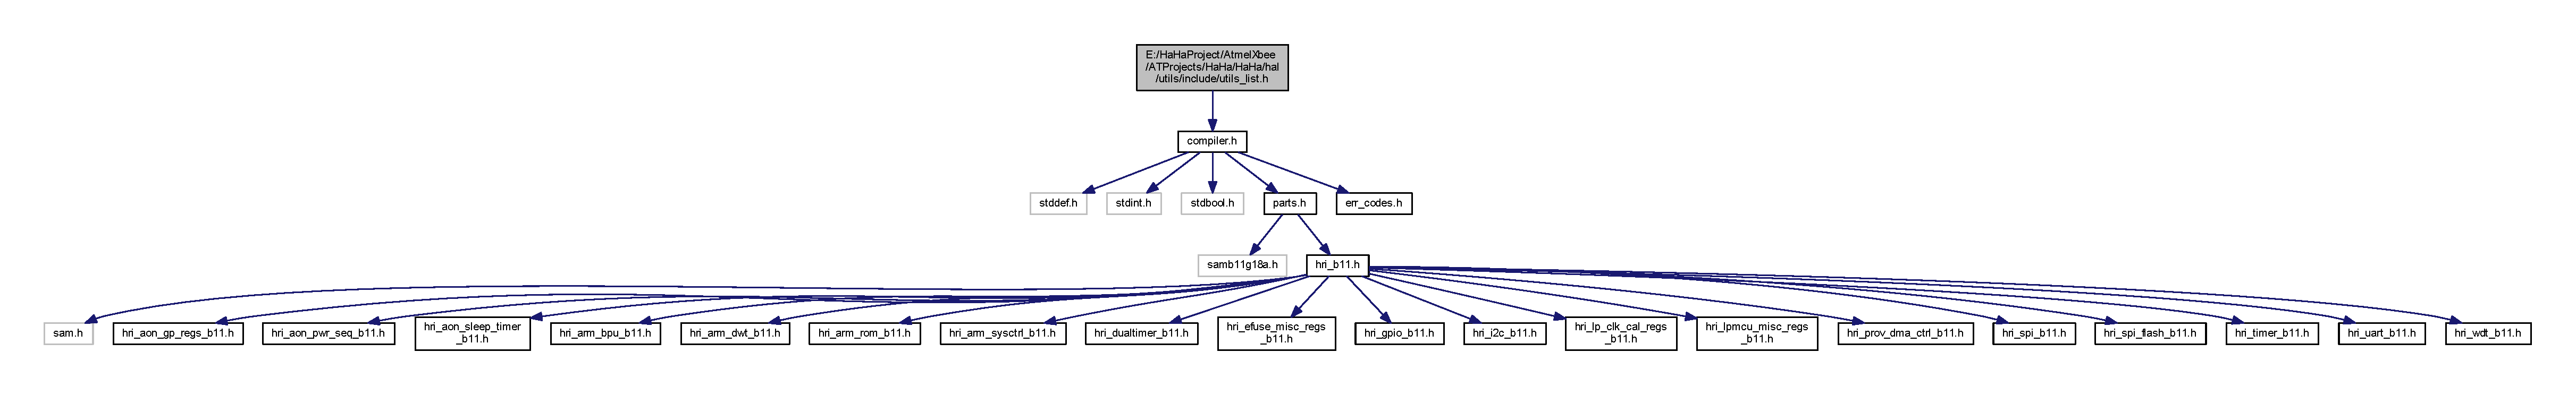
\includegraphics[width=350pt]{utils__list_8h__incl}
\end{center}
\end{figure}
This graph shows which files directly or indirectly include this file\+:\nopagebreak
\begin{figure}[H]
\begin{center}
\leavevmode
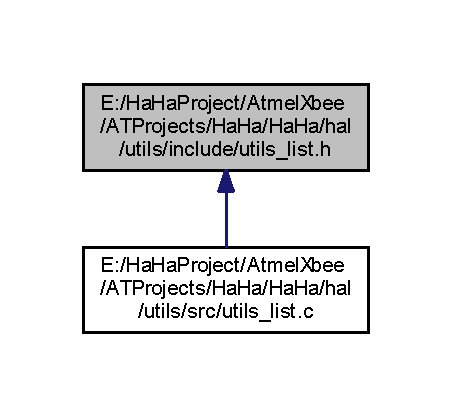
\includegraphics[width=217pt]{utils__list_8h__dep__incl}
\end{center}
\end{figure}
\subsection*{Classes}
\begin{DoxyCompactItemize}
\item 
struct \hyperlink{structlist__element}{list\+\_\+element}
\begin{DoxyCompactList}\small\item\em List element type. \end{DoxyCompactList}\item 
struct \hyperlink{structlist__descriptor}{list\+\_\+descriptor}
\begin{DoxyCompactList}\small\item\em List head type. \end{DoxyCompactList}\end{DoxyCompactItemize}
\subsection*{Functions}
\begin{DoxyCompactItemize}
\item 
void \hyperlink{group__doc__driver__hal__utils__list_gafb3237f00dbf55a40075f3a42c49d32a}{list\+\_\+insert\+\_\+as\+\_\+head} (struct \hyperlink{structlist__descriptor}{list\+\_\+descriptor} $\ast$const list, void $\ast$const element)
\begin{DoxyCompactList}\small\item\em Insert an element as list head. \end{DoxyCompactList}\item 
void \hyperlink{group__doc__driver__hal__utils__list_ga55b8c083fa131f829b1c998e14352f34}{list\+\_\+insert\+\_\+after} (void $\ast$const after, void $\ast$const element)
\begin{DoxyCompactList}\small\item\em Insert an element after the given list element. \end{DoxyCompactList}\item 
void \hyperlink{group__doc__driver__hal__utils__list_ga48c5a1a13223944dd190a6a028075deb}{list\+\_\+insert\+\_\+at\+\_\+end} (struct \hyperlink{structlist__descriptor}{list\+\_\+descriptor} $\ast$const list, void $\ast$const element)
\begin{DoxyCompactList}\small\item\em Insert an element at list end. \end{DoxyCompactList}\item 
bool \hyperlink{group__doc__driver__hal__utils__list_ga26022c1362f0fa7e17b734262229c1a7}{is\+\_\+list\+\_\+element} (const struct \hyperlink{structlist__descriptor}{list\+\_\+descriptor} $\ast$const list, const void $\ast$const element)
\begin{DoxyCompactList}\small\item\em Check whether an element belongs to a list. \end{DoxyCompactList}\item 
void $\ast$ \hyperlink{group__doc__driver__hal__utils__list_ga2269db44f7013963f60c568dd8d08022}{list\+\_\+remove\+\_\+head} (struct \hyperlink{structlist__descriptor}{list\+\_\+descriptor} $\ast$const list)
\begin{DoxyCompactList}\small\item\em Removes list head. \end{DoxyCompactList}\item 
bool \hyperlink{group__doc__driver__hal__utils__list_gad5a2a1ff5dcdfadb47d4ba436e154c98}{list\+\_\+delete\+\_\+element} (struct \hyperlink{structlist__descriptor}{list\+\_\+descriptor} $\ast$const list, const void $\ast$const element)
\begin{DoxyCompactList}\small\item\em Removes list element. \end{DoxyCompactList}\end{DoxyCompactItemize}


\subsection{Detailed Description}
List declaration. 

Copyright (C) 2014 Atmel Corporation. All rights reserved.
\hypertarget{utils__repeat__macro_8h}{}\section{E\+:/\+Ha\+Ha\+Project/\+Atmel\+Xbee/\+A\+T\+Projects/\+Ha\+Ha/\+Ha\+Ha/hal/utils/include/utils\+\_\+repeat\+\_\+macro.h File Reference}
\label{utils__repeat__macro_8h}\index{E\+:/\+Ha\+Ha\+Project/\+Atmel\+Xbee/\+A\+T\+Projects/\+Ha\+Ha/\+Ha\+Ha/hal/utils/include/utils\+\_\+repeat\+\_\+macro.\+h@{E\+:/\+Ha\+Ha\+Project/\+Atmel\+Xbee/\+A\+T\+Projects/\+Ha\+Ha/\+Ha\+Ha/hal/utils/include/utils\+\_\+repeat\+\_\+macro.\+h}}


Repeat macro.  


{\ttfamily \#include $<$utils\+\_\+increment\+\_\+macro.\+h$>$}\newline
Include dependency graph for utils\+\_\+repeat\+\_\+macro.\+h\+:
\nopagebreak
\begin{figure}[H]
\begin{center}
\leavevmode
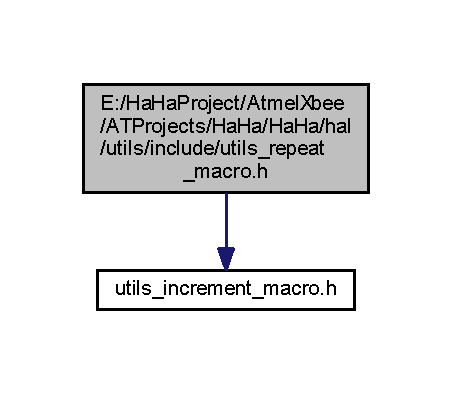
\includegraphics[width=217pt]{utils__repeat__macro_8h__incl}
\end{center}
\end{figure}
\subsection*{Macros}
\begin{DoxyCompactItemize}
\item 
\#define \hyperlink{utils__repeat__macro_8h_ad5f5e876b6f1c68b9822a0ea14fe1a6c}{R\+E\+P\+E\+A\+T\+\_\+\+M\+A\+C\+RO}(macro,  arg,  n)~\hyperlink{utils__repeat__macro_8h_ab09d7ad3a3f4651a80a51217be3f49c5}{R\+E\+P\+E\+A\+T\+\_\+\+M\+A\+C\+R\+O\+\_\+I}(macro, arg, n)
\item 
\#define \hyperlink{utils__repeat__macro_8h_ab09d7ad3a3f4651a80a51217be3f49c5}{R\+E\+P\+E\+A\+T\+\_\+\+M\+A\+C\+R\+O\+\_\+I}(macro,  arg,  n)~R\+E\+P\+E\+AT\#\#n(macro, arg, 0)
\item 
\#define \hyperlink{utils__repeat__macro_8h_adcac9030821ffa0f4416075c757faf33}{R\+E\+P\+E\+A\+T1}(macro,  arg,  n)~macro(arg, n)
\item 
\#define \hyperlink{utils__repeat__macro_8h_ae939ddcd63fb109cabd1dc49e783c1e2}{R\+E\+P\+E\+A\+T2}(macro,  arg,  n)~macro(arg, n) \hyperlink{utils__repeat__macro_8h_adcac9030821ffa0f4416075c757faf33}{R\+E\+P\+E\+A\+T1}(macro, arg, \hyperlink{utils__increment__macro_8h_a224df094eda9f558243c300cd524f8e8}{I\+N\+C\+\_\+\+V\+A\+L\+UE}(n))
\item 
\#define \hyperlink{utils__repeat__macro_8h_ae98f2b44468c41ec124d166822ab270e}{R\+E\+P\+E\+A\+T3}(macro,  arg,  n)~macro(arg, n) \hyperlink{utils__repeat__macro_8h_ae939ddcd63fb109cabd1dc49e783c1e2}{R\+E\+P\+E\+A\+T2}(macro, arg, \hyperlink{utils__increment__macro_8h_a224df094eda9f558243c300cd524f8e8}{I\+N\+C\+\_\+\+V\+A\+L\+UE}(n))
\item 
\#define \hyperlink{utils__repeat__macro_8h_afb8c5f37d5c8c4a93899881fb9a27561}{R\+E\+P\+E\+A\+T4}(macro,  arg,  n)~macro(arg, n) \hyperlink{utils__repeat__macro_8h_ae98f2b44468c41ec124d166822ab270e}{R\+E\+P\+E\+A\+T3}(macro, arg, \hyperlink{utils__increment__macro_8h_a224df094eda9f558243c300cd524f8e8}{I\+N\+C\+\_\+\+V\+A\+L\+UE}(n))
\item 
\#define \hyperlink{utils__repeat__macro_8h_a010de2317a5f7603a7fcafc884deb0a3}{R\+E\+P\+E\+A\+T5}(macro,  arg,  n)~macro(arg, n) \hyperlink{utils__repeat__macro_8h_afb8c5f37d5c8c4a93899881fb9a27561}{R\+E\+P\+E\+A\+T4}(macro, arg, \hyperlink{utils__increment__macro_8h_a224df094eda9f558243c300cd524f8e8}{I\+N\+C\+\_\+\+V\+A\+L\+UE}(n))
\item 
\#define \hyperlink{utils__repeat__macro_8h_aaaf40f1aca20f6dee0fc7cd3d9722145}{R\+E\+P\+E\+A\+T6}(macro,  arg,  n)~macro(arg, n) \hyperlink{utils__repeat__macro_8h_a010de2317a5f7603a7fcafc884deb0a3}{R\+E\+P\+E\+A\+T5}(macro, arg, \hyperlink{utils__increment__macro_8h_a224df094eda9f558243c300cd524f8e8}{I\+N\+C\+\_\+\+V\+A\+L\+UE}(n))
\item 
\#define \hyperlink{utils__repeat__macro_8h_a244a0881659ae5612a484d6d2e066a0a}{R\+E\+P\+E\+A\+T7}(macro,  arg,  n)~macro(arg, n) \hyperlink{utils__repeat__macro_8h_aaaf40f1aca20f6dee0fc7cd3d9722145}{R\+E\+P\+E\+A\+T6}(macro, arg, \hyperlink{utils__increment__macro_8h_a224df094eda9f558243c300cd524f8e8}{I\+N\+C\+\_\+\+V\+A\+L\+UE}(n))
\item 
\#define \hyperlink{utils__repeat__macro_8h_a5c648291c0dbe67f8bc7524478317513}{R\+E\+P\+E\+A\+T8}(macro,  arg,  n)~macro(arg, n) \hyperlink{utils__repeat__macro_8h_a244a0881659ae5612a484d6d2e066a0a}{R\+E\+P\+E\+A\+T7}(macro, arg, \hyperlink{utils__increment__macro_8h_a224df094eda9f558243c300cd524f8e8}{I\+N\+C\+\_\+\+V\+A\+L\+UE}(n))
\item 
\#define \hyperlink{utils__repeat__macro_8h_accc57b7c009572848102193f1e64bef1}{R\+E\+P\+E\+A\+T9}(macro,  arg,  n)~macro(arg, n) \hyperlink{utils__repeat__macro_8h_a5c648291c0dbe67f8bc7524478317513}{R\+E\+P\+E\+A\+T8}(macro, arg, \hyperlink{utils__increment__macro_8h_a224df094eda9f558243c300cd524f8e8}{I\+N\+C\+\_\+\+V\+A\+L\+UE}(n))
\item 
\#define \hyperlink{utils__repeat__macro_8h_a15e97021179f8bafe424042bd90b0fb2}{R\+E\+P\+E\+A\+T10}(macro,  arg,  n)~macro(arg, n) \hyperlink{utils__repeat__macro_8h_accc57b7c009572848102193f1e64bef1}{R\+E\+P\+E\+A\+T9}(macro, arg, \hyperlink{utils__increment__macro_8h_a224df094eda9f558243c300cd524f8e8}{I\+N\+C\+\_\+\+V\+A\+L\+UE}(n))
\item 
\#define \hyperlink{utils__repeat__macro_8h_a68e167c395baf3c25ce644b4a0f6662f}{R\+E\+P\+E\+A\+T11}(macro,  arg,  n)~macro(arg, n) \hyperlink{utils__repeat__macro_8h_a15e97021179f8bafe424042bd90b0fb2}{R\+E\+P\+E\+A\+T10}(macro, arg, \hyperlink{utils__increment__macro_8h_a224df094eda9f558243c300cd524f8e8}{I\+N\+C\+\_\+\+V\+A\+L\+UE}(n))
\item 
\#define \hyperlink{utils__repeat__macro_8h_a1ed7175c4651446e4caeb8668eb1a3df}{R\+E\+P\+E\+A\+T12}(macro,  arg,  n)~macro(arg, n) \hyperlink{utils__repeat__macro_8h_a68e167c395baf3c25ce644b4a0f6662f}{R\+E\+P\+E\+A\+T11}(macro, arg, \hyperlink{utils__increment__macro_8h_a224df094eda9f558243c300cd524f8e8}{I\+N\+C\+\_\+\+V\+A\+L\+UE}(n))
\item 
\#define \hyperlink{utils__repeat__macro_8h_adedaeb5868eabd61aa6e52a6acbc0d09}{R\+E\+P\+E\+A\+T13}(macro,  arg,  n)~macro(arg, n) \hyperlink{utils__repeat__macro_8h_a1ed7175c4651446e4caeb8668eb1a3df}{R\+E\+P\+E\+A\+T12}(macro, arg, \hyperlink{utils__increment__macro_8h_a224df094eda9f558243c300cd524f8e8}{I\+N\+C\+\_\+\+V\+A\+L\+UE}(n))
\item 
\#define \hyperlink{utils__repeat__macro_8h_afab6df5fda008d1c92241026f71df307}{R\+E\+P\+E\+A\+T14}(macro,  arg,  n)~macro(arg, n) \hyperlink{utils__repeat__macro_8h_adedaeb5868eabd61aa6e52a6acbc0d09}{R\+E\+P\+E\+A\+T13}(macro, arg, \hyperlink{utils__increment__macro_8h_a224df094eda9f558243c300cd524f8e8}{I\+N\+C\+\_\+\+V\+A\+L\+UE}(n))
\item 
\#define \hyperlink{utils__repeat__macro_8h_aac89c2700d769c3d2b883fafc9ec327a}{R\+E\+P\+E\+A\+T15}(macro,  arg,  n)~macro(arg, n) \hyperlink{utils__repeat__macro_8h_afab6df5fda008d1c92241026f71df307}{R\+E\+P\+E\+A\+T14}(macro, arg, \hyperlink{utils__increment__macro_8h_a224df094eda9f558243c300cd524f8e8}{I\+N\+C\+\_\+\+V\+A\+L\+UE}(n))
\item 
\#define \hyperlink{utils__repeat__macro_8h_af632550a6e63adc84f2b95d47de68551}{R\+E\+P\+E\+A\+T16}(macro,  arg,  n)~macro(arg, n) \hyperlink{utils__repeat__macro_8h_aac89c2700d769c3d2b883fafc9ec327a}{R\+E\+P\+E\+A\+T15}(macro, arg, \hyperlink{utils__increment__macro_8h_a224df094eda9f558243c300cd524f8e8}{I\+N\+C\+\_\+\+V\+A\+L\+UE}(n))
\item 
\#define \hyperlink{utils__repeat__macro_8h_a6caf58e071363c10f5c9528e2a36f1de}{R\+E\+P\+E\+A\+T17}(macro,  arg,  n)~macro(arg, n) \hyperlink{utils__repeat__macro_8h_af632550a6e63adc84f2b95d47de68551}{R\+E\+P\+E\+A\+T16}(macro, arg, \hyperlink{utils__increment__macro_8h_a224df094eda9f558243c300cd524f8e8}{I\+N\+C\+\_\+\+V\+A\+L\+UE}(n))
\item 
\#define \hyperlink{utils__repeat__macro_8h_ad79da6153458fd4573fe65f8e591561d}{R\+E\+P\+E\+A\+T18}(macro,  arg,  n)~macro(arg, n) \hyperlink{utils__repeat__macro_8h_a6caf58e071363c10f5c9528e2a36f1de}{R\+E\+P\+E\+A\+T17}(macro, arg, \hyperlink{utils__increment__macro_8h_a224df094eda9f558243c300cd524f8e8}{I\+N\+C\+\_\+\+V\+A\+L\+UE}(n))
\item 
\#define \hyperlink{utils__repeat__macro_8h_ab13a3c10f4e1ed8e49cc368e0f18b750}{R\+E\+P\+E\+A\+T19}(macro,  arg,  n)~macro(arg, n) \hyperlink{utils__repeat__macro_8h_ad79da6153458fd4573fe65f8e591561d}{R\+E\+P\+E\+A\+T18}(macro, arg, \hyperlink{utils__increment__macro_8h_a224df094eda9f558243c300cd524f8e8}{I\+N\+C\+\_\+\+V\+A\+L\+UE}(n))
\item 
\#define \hyperlink{utils__repeat__macro_8h_ac28838967e59812bcd23329ad8b97b09}{R\+E\+P\+E\+A\+T20}(macro,  arg,  n)~macro(arg, n) \hyperlink{utils__repeat__macro_8h_ab13a3c10f4e1ed8e49cc368e0f18b750}{R\+E\+P\+E\+A\+T19}(macro, arg, \hyperlink{utils__increment__macro_8h_a224df094eda9f558243c300cd524f8e8}{I\+N\+C\+\_\+\+V\+A\+L\+UE}(n))
\item 
\#define \hyperlink{utils__repeat__macro_8h_ae0ade3bd83923e14310e13cbbb3eeb0e}{R\+E\+P\+E\+A\+T21}(macro,  arg,  n)~macro(arg, n) \hyperlink{utils__repeat__macro_8h_ac28838967e59812bcd23329ad8b97b09}{R\+E\+P\+E\+A\+T20}(macro, arg, \hyperlink{utils__increment__macro_8h_a224df094eda9f558243c300cd524f8e8}{I\+N\+C\+\_\+\+V\+A\+L\+UE}(n))
\item 
\#define \hyperlink{utils__repeat__macro_8h_af96e644a6b3821de392115c540f27465}{R\+E\+P\+E\+A\+T22}(macro,  arg,  n)~macro(arg, n) \hyperlink{utils__repeat__macro_8h_ae0ade3bd83923e14310e13cbbb3eeb0e}{R\+E\+P\+E\+A\+T21}(macro, arg, \hyperlink{utils__increment__macro_8h_a224df094eda9f558243c300cd524f8e8}{I\+N\+C\+\_\+\+V\+A\+L\+UE}(n))
\item 
\#define \hyperlink{utils__repeat__macro_8h_a55e774a4904babe4a614a6bae8b1722c}{R\+E\+P\+E\+A\+T23}(macro,  arg,  n)~macro(arg, n) \hyperlink{utils__repeat__macro_8h_af96e644a6b3821de392115c540f27465}{R\+E\+P\+E\+A\+T22}(macro, arg, \hyperlink{utils__increment__macro_8h_a224df094eda9f558243c300cd524f8e8}{I\+N\+C\+\_\+\+V\+A\+L\+UE}(n))
\item 
\#define \hyperlink{utils__repeat__macro_8h_a48af842f8c05ba880a73f5f98086c66f}{R\+E\+P\+E\+A\+T24}(macro,  arg,  n)~macro(arg, n) \hyperlink{utils__repeat__macro_8h_a55e774a4904babe4a614a6bae8b1722c}{R\+E\+P\+E\+A\+T23}(macro, arg, \hyperlink{utils__increment__macro_8h_a224df094eda9f558243c300cd524f8e8}{I\+N\+C\+\_\+\+V\+A\+L\+UE}(n))
\item 
\#define \hyperlink{utils__repeat__macro_8h_ad493e9c85db2d739410a59d9cd9987dc}{R\+E\+P\+E\+A\+T25}(macro,  arg,  n)~macro(arg, n) \hyperlink{utils__repeat__macro_8h_a48af842f8c05ba880a73f5f98086c66f}{R\+E\+P\+E\+A\+T24}(macro, arg, \hyperlink{utils__increment__macro_8h_a224df094eda9f558243c300cd524f8e8}{I\+N\+C\+\_\+\+V\+A\+L\+UE}(n))
\item 
\#define \hyperlink{utils__repeat__macro_8h_a47abe94a450227be4604e7537d3c7617}{R\+E\+P\+E\+A\+T26}(macro,  arg,  n)~macro(arg, n) \hyperlink{utils__repeat__macro_8h_ad493e9c85db2d739410a59d9cd9987dc}{R\+E\+P\+E\+A\+T25}(macro, arg, \hyperlink{utils__increment__macro_8h_a224df094eda9f558243c300cd524f8e8}{I\+N\+C\+\_\+\+V\+A\+L\+UE}(n))
\item 
\#define \hyperlink{utils__repeat__macro_8h_a3f91b71e4c97fd0059e2c3c86ea5266c}{R\+E\+P\+E\+A\+T27}(macro,  arg,  n)~macro(arg, n) \hyperlink{utils__repeat__macro_8h_a47abe94a450227be4604e7537d3c7617}{R\+E\+P\+E\+A\+T26}(macro, arg, \hyperlink{utils__increment__macro_8h_a224df094eda9f558243c300cd524f8e8}{I\+N\+C\+\_\+\+V\+A\+L\+UE}(n))
\item 
\#define \hyperlink{utils__repeat__macro_8h_af895914bbd2a4c78d74e2092de96a1c0}{R\+E\+P\+E\+A\+T28}(macro,  arg,  n)~macro(arg, n) \hyperlink{utils__repeat__macro_8h_a3f91b71e4c97fd0059e2c3c86ea5266c}{R\+E\+P\+E\+A\+T27}(macro, arg, \hyperlink{utils__increment__macro_8h_a224df094eda9f558243c300cd524f8e8}{I\+N\+C\+\_\+\+V\+A\+L\+UE}(n))
\item 
\#define \hyperlink{utils__repeat__macro_8h_a0b1daf2fd3b371fcb735abf0b3fa274f}{R\+E\+P\+E\+A\+T29}(macro,  arg,  n)~macro(arg, n) \hyperlink{utils__repeat__macro_8h_af895914bbd2a4c78d74e2092de96a1c0}{R\+E\+P\+E\+A\+T28}(macro, arg, \hyperlink{utils__increment__macro_8h_a224df094eda9f558243c300cd524f8e8}{I\+N\+C\+\_\+\+V\+A\+L\+UE}(n))
\item 
\#define \hyperlink{utils__repeat__macro_8h_ad666bda4ae817b2941a7be72edfca269}{R\+E\+P\+E\+A\+T30}(macro,  arg,  n)~macro(arg, n) \hyperlink{utils__repeat__macro_8h_a0b1daf2fd3b371fcb735abf0b3fa274f}{R\+E\+P\+E\+A\+T29}(macro, arg, \hyperlink{utils__increment__macro_8h_a224df094eda9f558243c300cd524f8e8}{I\+N\+C\+\_\+\+V\+A\+L\+UE}(n))
\item 
\#define \hyperlink{utils__repeat__macro_8h_a5607b9709ab0bc6a65d4294dd58401c0}{R\+E\+P\+E\+A\+T31}(macro,  arg,  n)~macro(arg, n) \hyperlink{utils__repeat__macro_8h_ad666bda4ae817b2941a7be72edfca269}{R\+E\+P\+E\+A\+T30}(macro, arg, \hyperlink{utils__increment__macro_8h_a224df094eda9f558243c300cd524f8e8}{I\+N\+C\+\_\+\+V\+A\+L\+UE}(n))
\item 
\#define \hyperlink{utils__repeat__macro_8h_a2176d28ea971bd334c90cc5c66a6f17b}{R\+E\+P\+E\+A\+T32}(macro,  arg,  n)~macro(arg, n) \hyperlink{utils__repeat__macro_8h_a5607b9709ab0bc6a65d4294dd58401c0}{R\+E\+P\+E\+A\+T31}(macro, arg, \hyperlink{utils__increment__macro_8h_a224df094eda9f558243c300cd524f8e8}{I\+N\+C\+\_\+\+V\+A\+L\+UE}(n))
\item 
\#define \hyperlink{utils__repeat__macro_8h_afdb2c442636c56895dfa099aea05cea9}{R\+E\+P\+E\+A\+T33}(macro,  arg,  n)~macro(arg, n) \hyperlink{utils__repeat__macro_8h_a2176d28ea971bd334c90cc5c66a6f17b}{R\+E\+P\+E\+A\+T32}(macro, arg, \hyperlink{utils__increment__macro_8h_a224df094eda9f558243c300cd524f8e8}{I\+N\+C\+\_\+\+V\+A\+L\+UE}(n))
\item 
\#define \hyperlink{utils__repeat__macro_8h_a8117476176f5001592b4e74a7bc37825}{R\+E\+P\+E\+A\+T34}(macro,  arg,  n)~macro(arg, n) \hyperlink{utils__repeat__macro_8h_afdb2c442636c56895dfa099aea05cea9}{R\+E\+P\+E\+A\+T33}(macro, arg, \hyperlink{utils__increment__macro_8h_a224df094eda9f558243c300cd524f8e8}{I\+N\+C\+\_\+\+V\+A\+L\+UE}(n))
\item 
\#define \hyperlink{utils__repeat__macro_8h_abab333e9f0fc903682bfdb2f44343a5c}{R\+E\+P\+E\+A\+T35}(macro,  arg,  n)~macro(arg, n) \hyperlink{utils__repeat__macro_8h_a8117476176f5001592b4e74a7bc37825}{R\+E\+P\+E\+A\+T34}(macro, arg, \hyperlink{utils__increment__macro_8h_a224df094eda9f558243c300cd524f8e8}{I\+N\+C\+\_\+\+V\+A\+L\+UE}(n))
\item 
\#define \hyperlink{utils__repeat__macro_8h_a737f87e48217e27b65564d56195f876c}{R\+E\+P\+E\+A\+T36}(macro,  arg,  n)~macro(arg, n) \hyperlink{utils__repeat__macro_8h_abab333e9f0fc903682bfdb2f44343a5c}{R\+E\+P\+E\+A\+T35}(macro, arg, \hyperlink{utils__increment__macro_8h_a224df094eda9f558243c300cd524f8e8}{I\+N\+C\+\_\+\+V\+A\+L\+UE}(n))
\item 
\#define \hyperlink{utils__repeat__macro_8h_aef481e96e48ae589cd77a06596fcfe5b}{R\+E\+P\+E\+A\+T37}(macro,  arg,  n)~macro(arg, n) \hyperlink{utils__repeat__macro_8h_a737f87e48217e27b65564d56195f876c}{R\+E\+P\+E\+A\+T36}(macro, arg, \hyperlink{utils__increment__macro_8h_a224df094eda9f558243c300cd524f8e8}{I\+N\+C\+\_\+\+V\+A\+L\+UE}(n))
\item 
\#define \hyperlink{utils__repeat__macro_8h_abc47c3574272076c2ec933822ec19741}{R\+E\+P\+E\+A\+T38}(macro,  arg,  n)~macro(arg, n) \hyperlink{utils__repeat__macro_8h_aef481e96e48ae589cd77a06596fcfe5b}{R\+E\+P\+E\+A\+T37}(macro, arg, \hyperlink{utils__increment__macro_8h_a224df094eda9f558243c300cd524f8e8}{I\+N\+C\+\_\+\+V\+A\+L\+UE}(n))
\item 
\#define \hyperlink{utils__repeat__macro_8h_afda89af7c2f15a0b5177b855453758de}{R\+E\+P\+E\+A\+T39}(macro,  arg,  n)~macro(arg, n) \hyperlink{utils__repeat__macro_8h_abc47c3574272076c2ec933822ec19741}{R\+E\+P\+E\+A\+T38}(macro, arg, \hyperlink{utils__increment__macro_8h_a224df094eda9f558243c300cd524f8e8}{I\+N\+C\+\_\+\+V\+A\+L\+UE}(n))
\item 
\#define \hyperlink{utils__repeat__macro_8h_afc5732cb8f55a5d69619c7e2b1420f3c}{R\+E\+P\+E\+A\+T40}(macro,  arg,  n)~macro(arg, n) \hyperlink{utils__repeat__macro_8h_afda89af7c2f15a0b5177b855453758de}{R\+E\+P\+E\+A\+T39}(macro, arg, \hyperlink{utils__increment__macro_8h_a224df094eda9f558243c300cd524f8e8}{I\+N\+C\+\_\+\+V\+A\+L\+UE}(n))
\item 
\#define \hyperlink{utils__repeat__macro_8h_adb8f4478112f4acfc4c70fb49de4dea8}{R\+E\+P\+E\+A\+T41}(macro,  arg,  n)~macro(arg, n) \hyperlink{utils__repeat__macro_8h_afc5732cb8f55a5d69619c7e2b1420f3c}{R\+E\+P\+E\+A\+T40}(macro, arg, \hyperlink{utils__increment__macro_8h_a224df094eda9f558243c300cd524f8e8}{I\+N\+C\+\_\+\+V\+A\+L\+UE}(n))
\item 
\#define \hyperlink{utils__repeat__macro_8h_a50172e846fbaabf3720eb850eadb7d98}{R\+E\+P\+E\+A\+T42}(macro,  arg,  n)~macro(arg, n) \hyperlink{utils__repeat__macro_8h_adb8f4478112f4acfc4c70fb49de4dea8}{R\+E\+P\+E\+A\+T41}(macro, arg, \hyperlink{utils__increment__macro_8h_a224df094eda9f558243c300cd524f8e8}{I\+N\+C\+\_\+\+V\+A\+L\+UE}(n))
\item 
\#define \hyperlink{utils__repeat__macro_8h_a50250731df225a0187fede9bb5c8d5f1}{R\+E\+P\+E\+A\+T43}(macro,  arg,  n)~macro(arg, n) \hyperlink{utils__repeat__macro_8h_a50172e846fbaabf3720eb850eadb7d98}{R\+E\+P\+E\+A\+T42}(macro, arg, \hyperlink{utils__increment__macro_8h_a224df094eda9f558243c300cd524f8e8}{I\+N\+C\+\_\+\+V\+A\+L\+UE}(n))
\item 
\#define \hyperlink{utils__repeat__macro_8h_a4b74b2e82393f8fefd3f4570bc981faa}{R\+E\+P\+E\+A\+T44}(macro,  arg,  n)~macro(arg, n) \hyperlink{utils__repeat__macro_8h_a50250731df225a0187fede9bb5c8d5f1}{R\+E\+P\+E\+A\+T43}(macro, arg, \hyperlink{utils__increment__macro_8h_a224df094eda9f558243c300cd524f8e8}{I\+N\+C\+\_\+\+V\+A\+L\+UE}(n))
\item 
\#define \hyperlink{utils__repeat__macro_8h_ae7ccdfb909133a3c284715b33ac583b3}{R\+E\+P\+E\+A\+T45}(macro,  arg,  n)~macro(arg, n) \hyperlink{utils__repeat__macro_8h_a4b74b2e82393f8fefd3f4570bc981faa}{R\+E\+P\+E\+A\+T44}(macro, arg, \hyperlink{utils__increment__macro_8h_a224df094eda9f558243c300cd524f8e8}{I\+N\+C\+\_\+\+V\+A\+L\+UE}(n))
\item 
\#define \hyperlink{utils__repeat__macro_8h_a2656637b9dfce03608f95ee4ed64fd8d}{R\+E\+P\+E\+A\+T46}(macro,  arg,  n)~macro(arg, n) \hyperlink{utils__repeat__macro_8h_ae7ccdfb909133a3c284715b33ac583b3}{R\+E\+P\+E\+A\+T45}(macro, arg, \hyperlink{utils__increment__macro_8h_a224df094eda9f558243c300cd524f8e8}{I\+N\+C\+\_\+\+V\+A\+L\+UE}(n))
\item 
\#define \hyperlink{utils__repeat__macro_8h_ac152945a2193d92d18e8d9b1887b98ff}{R\+E\+P\+E\+A\+T47}(macro,  arg,  n)~macro(arg, n) \hyperlink{utils__repeat__macro_8h_a2656637b9dfce03608f95ee4ed64fd8d}{R\+E\+P\+E\+A\+T46}(macro, arg, \hyperlink{utils__increment__macro_8h_a224df094eda9f558243c300cd524f8e8}{I\+N\+C\+\_\+\+V\+A\+L\+UE}(n))
\item 
\#define \hyperlink{utils__repeat__macro_8h_ab6a493dc7b7a169be9f737829c6512a5}{R\+E\+P\+E\+A\+T48}(macro,  arg,  n)~macro(arg, n) \hyperlink{utils__repeat__macro_8h_ac152945a2193d92d18e8d9b1887b98ff}{R\+E\+P\+E\+A\+T47}(macro, arg, \hyperlink{utils__increment__macro_8h_a224df094eda9f558243c300cd524f8e8}{I\+N\+C\+\_\+\+V\+A\+L\+UE}(n))
\item 
\#define \hyperlink{utils__repeat__macro_8h_adddf0bc5e13278b1c37bbef195712e1f}{R\+E\+P\+E\+A\+T49}(macro,  arg,  n)~macro(arg, n) \hyperlink{utils__repeat__macro_8h_ab6a493dc7b7a169be9f737829c6512a5}{R\+E\+P\+E\+A\+T48}(macro, arg, \hyperlink{utils__increment__macro_8h_a224df094eda9f558243c300cd524f8e8}{I\+N\+C\+\_\+\+V\+A\+L\+UE}(n))
\item 
\#define \hyperlink{utils__repeat__macro_8h_ab29971c1ce816f8d3c9e3b42d37c27e1}{R\+E\+P\+E\+A\+T50}(macro,  arg,  n)~macro(arg, n) \hyperlink{utils__repeat__macro_8h_adddf0bc5e13278b1c37bbef195712e1f}{R\+E\+P\+E\+A\+T49}(macro, arg, \hyperlink{utils__increment__macro_8h_a224df094eda9f558243c300cd524f8e8}{I\+N\+C\+\_\+\+V\+A\+L\+UE}(n))
\item 
\#define \hyperlink{utils__repeat__macro_8h_a2d4f2cc133866cee9a375f7e7285b90d}{R\+E\+P\+E\+A\+T51}(macro,  arg,  n)~macro(arg, n) \hyperlink{utils__repeat__macro_8h_ab29971c1ce816f8d3c9e3b42d37c27e1}{R\+E\+P\+E\+A\+T50}(macro, arg, \hyperlink{utils__increment__macro_8h_a224df094eda9f558243c300cd524f8e8}{I\+N\+C\+\_\+\+V\+A\+L\+UE}(n))
\item 
\#define \hyperlink{utils__repeat__macro_8h_acde8d89f807d68922c304884b659656c}{R\+E\+P\+E\+A\+T52}(macro,  arg,  n)~macro(arg, n) \hyperlink{utils__repeat__macro_8h_a2d4f2cc133866cee9a375f7e7285b90d}{R\+E\+P\+E\+A\+T51}(macro, arg, \hyperlink{utils__increment__macro_8h_a224df094eda9f558243c300cd524f8e8}{I\+N\+C\+\_\+\+V\+A\+L\+UE}(n))
\item 
\#define \hyperlink{utils__repeat__macro_8h_a26dd48f60a9e62b0388c0a65c808c98e}{R\+E\+P\+E\+A\+T53}(macro,  arg,  n)~macro(arg, n) \hyperlink{utils__repeat__macro_8h_acde8d89f807d68922c304884b659656c}{R\+E\+P\+E\+A\+T52}(macro, arg, \hyperlink{utils__increment__macro_8h_a224df094eda9f558243c300cd524f8e8}{I\+N\+C\+\_\+\+V\+A\+L\+UE}(n))
\item 
\#define \hyperlink{utils__repeat__macro_8h_aaf5fe2e3691bbb52c55965ed81a0f915}{R\+E\+P\+E\+A\+T54}(macro,  arg,  n)~macro(arg, n) \hyperlink{utils__repeat__macro_8h_a26dd48f60a9e62b0388c0a65c808c98e}{R\+E\+P\+E\+A\+T53}(macro, arg, \hyperlink{utils__increment__macro_8h_a224df094eda9f558243c300cd524f8e8}{I\+N\+C\+\_\+\+V\+A\+L\+UE}(n))
\item 
\#define \hyperlink{utils__repeat__macro_8h_a4c46f7c7545c5f0f70aed2972e8095e2}{R\+E\+P\+E\+A\+T55}(macro,  arg,  n)~macro(arg, n) \hyperlink{utils__repeat__macro_8h_aaf5fe2e3691bbb52c55965ed81a0f915}{R\+E\+P\+E\+A\+T54}(macro, arg, \hyperlink{utils__increment__macro_8h_a224df094eda9f558243c300cd524f8e8}{I\+N\+C\+\_\+\+V\+A\+L\+UE}(n))
\item 
\#define \hyperlink{utils__repeat__macro_8h_aa5ba4c771fa8ac9c9aa5149454c498eb}{R\+E\+P\+E\+A\+T56}(macro,  arg,  n)~macro(arg, n) \hyperlink{utils__repeat__macro_8h_a4c46f7c7545c5f0f70aed2972e8095e2}{R\+E\+P\+E\+A\+T55}(macro, arg, \hyperlink{utils__increment__macro_8h_a224df094eda9f558243c300cd524f8e8}{I\+N\+C\+\_\+\+V\+A\+L\+UE}(n))
\item 
\#define \hyperlink{utils__repeat__macro_8h_a19a2f6b7e6969cacc6087d20ea7b4051}{R\+E\+P\+E\+A\+T57}(macro,  arg,  n)~macro(arg, n) \hyperlink{utils__repeat__macro_8h_aa5ba4c771fa8ac9c9aa5149454c498eb}{R\+E\+P\+E\+A\+T56}(macro, arg, \hyperlink{utils__increment__macro_8h_a224df094eda9f558243c300cd524f8e8}{I\+N\+C\+\_\+\+V\+A\+L\+UE}(n))
\item 
\#define \hyperlink{utils__repeat__macro_8h_aff660cb8b838ba18b4ca0f96a0c23156}{R\+E\+P\+E\+A\+T58}(macro,  arg,  n)~macro(arg, n) \hyperlink{utils__repeat__macro_8h_a19a2f6b7e6969cacc6087d20ea7b4051}{R\+E\+P\+E\+A\+T57}(macro, arg, \hyperlink{utils__increment__macro_8h_a224df094eda9f558243c300cd524f8e8}{I\+N\+C\+\_\+\+V\+A\+L\+UE}(n))
\item 
\#define \hyperlink{utils__repeat__macro_8h_a0d1eafa018e9f9aeba4e3e9bb90a7322}{R\+E\+P\+E\+A\+T59}(macro,  arg,  n)~macro(arg, n) \hyperlink{utils__repeat__macro_8h_aff660cb8b838ba18b4ca0f96a0c23156}{R\+E\+P\+E\+A\+T58}(macro, arg, \hyperlink{utils__increment__macro_8h_a224df094eda9f558243c300cd524f8e8}{I\+N\+C\+\_\+\+V\+A\+L\+UE}(n))
\item 
\#define \hyperlink{utils__repeat__macro_8h_abdb65a2e563fdddd18868cca8350d3a0}{R\+E\+P\+E\+A\+T60}(macro,  arg,  n)~macro(arg, n) \hyperlink{utils__repeat__macro_8h_a0d1eafa018e9f9aeba4e3e9bb90a7322}{R\+E\+P\+E\+A\+T59}(macro, arg, \hyperlink{utils__increment__macro_8h_a224df094eda9f558243c300cd524f8e8}{I\+N\+C\+\_\+\+V\+A\+L\+UE}(n))
\item 
\#define \hyperlink{utils__repeat__macro_8h_a71554be0ff4eea1224d692f88d7eb00f}{R\+E\+P\+E\+A\+T61}(macro,  arg,  n)~macro(arg, n) \hyperlink{utils__repeat__macro_8h_abdb65a2e563fdddd18868cca8350d3a0}{R\+E\+P\+E\+A\+T60}(macro, arg, \hyperlink{utils__increment__macro_8h_a224df094eda9f558243c300cd524f8e8}{I\+N\+C\+\_\+\+V\+A\+L\+UE}(n))
\item 
\#define \hyperlink{utils__repeat__macro_8h_ad436e7b81a5cd3520f7660c91ce61deb}{R\+E\+P\+E\+A\+T62}(macro,  arg,  n)~macro(arg, n) \hyperlink{utils__repeat__macro_8h_a71554be0ff4eea1224d692f88d7eb00f}{R\+E\+P\+E\+A\+T61}(macro, arg, \hyperlink{utils__increment__macro_8h_a224df094eda9f558243c300cd524f8e8}{I\+N\+C\+\_\+\+V\+A\+L\+UE}(n))
\item 
\#define \hyperlink{utils__repeat__macro_8h_a2be36004c6352b53af077b884bae0883}{R\+E\+P\+E\+A\+T63}(macro,  arg,  n)~macro(arg, n) \hyperlink{utils__repeat__macro_8h_ad436e7b81a5cd3520f7660c91ce61deb}{R\+E\+P\+E\+A\+T62}(macro, arg, \hyperlink{utils__increment__macro_8h_a224df094eda9f558243c300cd524f8e8}{I\+N\+C\+\_\+\+V\+A\+L\+UE}(n))
\item 
\#define \hyperlink{utils__repeat__macro_8h_ad49e31951e9fd27e564defddfe9c81ee}{R\+E\+P\+E\+A\+T64}(macro,  arg,  n)~macro(arg, n) \hyperlink{utils__repeat__macro_8h_a2be36004c6352b53af077b884bae0883}{R\+E\+P\+E\+A\+T63}(macro, arg, \hyperlink{utils__increment__macro_8h_a224df094eda9f558243c300cd524f8e8}{I\+N\+C\+\_\+\+V\+A\+L\+UE}(n))
\item 
\#define \hyperlink{utils__repeat__macro_8h_a4b751baaa8075b667f7f8c8a52daa5a7}{R\+E\+P\+E\+A\+T65}(macro,  arg,  n)~macro(arg, n) \hyperlink{utils__repeat__macro_8h_ad49e31951e9fd27e564defddfe9c81ee}{R\+E\+P\+E\+A\+T64}(macro, arg, \hyperlink{utils__increment__macro_8h_a224df094eda9f558243c300cd524f8e8}{I\+N\+C\+\_\+\+V\+A\+L\+UE}(n))
\item 
\#define \hyperlink{utils__repeat__macro_8h_a0c62d92c9a9e6753a681590a11544215}{R\+E\+P\+E\+A\+T66}(macro,  arg,  n)~macro(arg, n) \hyperlink{utils__repeat__macro_8h_a4b751baaa8075b667f7f8c8a52daa5a7}{R\+E\+P\+E\+A\+T65}(macro, arg, \hyperlink{utils__increment__macro_8h_a224df094eda9f558243c300cd524f8e8}{I\+N\+C\+\_\+\+V\+A\+L\+UE}(n))
\item 
\#define \hyperlink{utils__repeat__macro_8h_ab8dc631230133d1fa0b8472e8399c0e8}{R\+E\+P\+E\+A\+T67}(macro,  arg,  n)~macro(arg, n) \hyperlink{utils__repeat__macro_8h_a0c62d92c9a9e6753a681590a11544215}{R\+E\+P\+E\+A\+T66}(macro, arg, \hyperlink{utils__increment__macro_8h_a224df094eda9f558243c300cd524f8e8}{I\+N\+C\+\_\+\+V\+A\+L\+UE}(n))
\item 
\#define \hyperlink{utils__repeat__macro_8h_a5527c88e1c50b10d626c42513cb400b9}{R\+E\+P\+E\+A\+T68}(macro,  arg,  n)~macro(arg, n) \hyperlink{utils__repeat__macro_8h_ab8dc631230133d1fa0b8472e8399c0e8}{R\+E\+P\+E\+A\+T67}(macro, arg, \hyperlink{utils__increment__macro_8h_a224df094eda9f558243c300cd524f8e8}{I\+N\+C\+\_\+\+V\+A\+L\+UE}(n))
\item 
\#define \hyperlink{utils__repeat__macro_8h_a9d875afb5bc183e655c131a599820577}{R\+E\+P\+E\+A\+T69}(macro,  arg,  n)~macro(arg, n) \hyperlink{utils__repeat__macro_8h_a5527c88e1c50b10d626c42513cb400b9}{R\+E\+P\+E\+A\+T68}(macro, arg, \hyperlink{utils__increment__macro_8h_a224df094eda9f558243c300cd524f8e8}{I\+N\+C\+\_\+\+V\+A\+L\+UE}(n))
\item 
\#define \hyperlink{utils__repeat__macro_8h_acbe877f68e116977b960b94ddbd84ea1}{R\+E\+P\+E\+A\+T70}(macro,  arg,  n)~macro(arg, n) \hyperlink{utils__repeat__macro_8h_a9d875afb5bc183e655c131a599820577}{R\+E\+P\+E\+A\+T69}(macro, arg, \hyperlink{utils__increment__macro_8h_a224df094eda9f558243c300cd524f8e8}{I\+N\+C\+\_\+\+V\+A\+L\+UE}(n))
\item 
\#define \hyperlink{utils__repeat__macro_8h_a72436e36cf8444a0aed9bd43c1d8ef24}{R\+E\+P\+E\+A\+T71}(macro,  arg,  n)~macro(arg, n) \hyperlink{utils__repeat__macro_8h_acbe877f68e116977b960b94ddbd84ea1}{R\+E\+P\+E\+A\+T70}(macro, arg, \hyperlink{utils__increment__macro_8h_a224df094eda9f558243c300cd524f8e8}{I\+N\+C\+\_\+\+V\+A\+L\+UE}(n))
\item 
\#define \hyperlink{utils__repeat__macro_8h_a2ffb97383da8a7513a79433955d8a2e3}{R\+E\+P\+E\+A\+T72}(macro,  arg,  n)~macro(arg, n) \hyperlink{utils__repeat__macro_8h_a72436e36cf8444a0aed9bd43c1d8ef24}{R\+E\+P\+E\+A\+T71}(macro, arg, \hyperlink{utils__increment__macro_8h_a224df094eda9f558243c300cd524f8e8}{I\+N\+C\+\_\+\+V\+A\+L\+UE}(n))
\item 
\#define \hyperlink{utils__repeat__macro_8h_a52b11bc1246436a6a9251de18df9d4b2}{R\+E\+P\+E\+A\+T73}(macro,  arg,  n)~macro(arg, n) \hyperlink{utils__repeat__macro_8h_a2ffb97383da8a7513a79433955d8a2e3}{R\+E\+P\+E\+A\+T72}(macro, arg, \hyperlink{utils__increment__macro_8h_a224df094eda9f558243c300cd524f8e8}{I\+N\+C\+\_\+\+V\+A\+L\+UE}(n))
\item 
\#define \hyperlink{utils__repeat__macro_8h_abb7230078243b05e32444a62dbc67a2e}{R\+E\+P\+E\+A\+T74}(macro,  arg,  n)~macro(arg, n) \hyperlink{utils__repeat__macro_8h_a52b11bc1246436a6a9251de18df9d4b2}{R\+E\+P\+E\+A\+T73}(macro, arg, \hyperlink{utils__increment__macro_8h_a224df094eda9f558243c300cd524f8e8}{I\+N\+C\+\_\+\+V\+A\+L\+UE}(n))
\item 
\#define \hyperlink{utils__repeat__macro_8h_a8a776454bd6242fc434f00ad5a634969}{R\+E\+P\+E\+A\+T75}(macro,  arg,  n)~macro(arg, n) \hyperlink{utils__repeat__macro_8h_abb7230078243b05e32444a62dbc67a2e}{R\+E\+P\+E\+A\+T74}(macro, arg, \hyperlink{utils__increment__macro_8h_a224df094eda9f558243c300cd524f8e8}{I\+N\+C\+\_\+\+V\+A\+L\+UE}(n))
\item 
\#define \hyperlink{utils__repeat__macro_8h_ae20227662cca1b4d23b8a880b91bdb49}{R\+E\+P\+E\+A\+T76}(macro,  arg,  n)~macro(arg, n) \hyperlink{utils__repeat__macro_8h_a8a776454bd6242fc434f00ad5a634969}{R\+E\+P\+E\+A\+T75}(macro, arg, \hyperlink{utils__increment__macro_8h_a224df094eda9f558243c300cd524f8e8}{I\+N\+C\+\_\+\+V\+A\+L\+UE}(n))
\item 
\#define \hyperlink{utils__repeat__macro_8h_a281df3fa2a49b7ada1d8bd606f3ad532}{R\+E\+P\+E\+A\+T77}(macro,  arg,  n)~macro(arg, n) \hyperlink{utils__repeat__macro_8h_ae20227662cca1b4d23b8a880b91bdb49}{R\+E\+P\+E\+A\+T76}(macro, arg, \hyperlink{utils__increment__macro_8h_a224df094eda9f558243c300cd524f8e8}{I\+N\+C\+\_\+\+V\+A\+L\+UE}(n))
\item 
\#define \hyperlink{utils__repeat__macro_8h_af5f97b0875d9c48d9af63df1893ed0f4}{R\+E\+P\+E\+A\+T78}(macro,  arg,  n)~macro(arg, n) \hyperlink{utils__repeat__macro_8h_a281df3fa2a49b7ada1d8bd606f3ad532}{R\+E\+P\+E\+A\+T77}(macro, arg, \hyperlink{utils__increment__macro_8h_a224df094eda9f558243c300cd524f8e8}{I\+N\+C\+\_\+\+V\+A\+L\+UE}(n))
\item 
\#define \hyperlink{utils__repeat__macro_8h_ad8114f5d91fa14ef82af3b94d0855a3e}{R\+E\+P\+E\+A\+T79}(macro,  arg,  n)~macro(arg, n) \hyperlink{utils__repeat__macro_8h_af5f97b0875d9c48d9af63df1893ed0f4}{R\+E\+P\+E\+A\+T78}(macro, arg, \hyperlink{utils__increment__macro_8h_a224df094eda9f558243c300cd524f8e8}{I\+N\+C\+\_\+\+V\+A\+L\+UE}(n))
\item 
\#define \hyperlink{utils__repeat__macro_8h_a17ef0409a24ef1473b1f37158b5dab24}{R\+E\+P\+E\+A\+T80}(macro,  arg,  n)~macro(arg, n) \hyperlink{utils__repeat__macro_8h_ad8114f5d91fa14ef82af3b94d0855a3e}{R\+E\+P\+E\+A\+T79}(macro, arg, \hyperlink{utils__increment__macro_8h_a224df094eda9f558243c300cd524f8e8}{I\+N\+C\+\_\+\+V\+A\+L\+UE}(n))
\item 
\#define \hyperlink{utils__repeat__macro_8h_a03c7f2e738976c8509566664ea7d9514}{R\+E\+P\+E\+A\+T81}(macro,  arg,  n)~macro(arg, n) \hyperlink{utils__repeat__macro_8h_a17ef0409a24ef1473b1f37158b5dab24}{R\+E\+P\+E\+A\+T80}(macro, arg, \hyperlink{utils__increment__macro_8h_a224df094eda9f558243c300cd524f8e8}{I\+N\+C\+\_\+\+V\+A\+L\+UE}(n))
\item 
\#define \hyperlink{utils__repeat__macro_8h_a487034858f15909a7848a7313c64c86c}{R\+E\+P\+E\+A\+T82}(macro,  arg,  n)~macro(arg, n) \hyperlink{utils__repeat__macro_8h_a03c7f2e738976c8509566664ea7d9514}{R\+E\+P\+E\+A\+T81}(macro, arg, \hyperlink{utils__increment__macro_8h_a224df094eda9f558243c300cd524f8e8}{I\+N\+C\+\_\+\+V\+A\+L\+UE}(n))
\item 
\#define \hyperlink{utils__repeat__macro_8h_a0a98b17b5f5bffb6af1084e10fcfa5a6}{R\+E\+P\+E\+A\+T83}(macro,  arg,  n)~macro(arg, n) \hyperlink{utils__repeat__macro_8h_a487034858f15909a7848a7313c64c86c}{R\+E\+P\+E\+A\+T82}(macro, arg, \hyperlink{utils__increment__macro_8h_a224df094eda9f558243c300cd524f8e8}{I\+N\+C\+\_\+\+V\+A\+L\+UE}(n))
\item 
\#define \hyperlink{utils__repeat__macro_8h_a16f5cd524781c55b6d8115c172480fe8}{R\+E\+P\+E\+A\+T84}(macro,  arg,  n)~macro(arg, n) \hyperlink{utils__repeat__macro_8h_a0a98b17b5f5bffb6af1084e10fcfa5a6}{R\+E\+P\+E\+A\+T83}(macro, arg, \hyperlink{utils__increment__macro_8h_a224df094eda9f558243c300cd524f8e8}{I\+N\+C\+\_\+\+V\+A\+L\+UE}(n))
\item 
\#define \hyperlink{utils__repeat__macro_8h_ae9c55018c9e39101216c829cc8a16209}{R\+E\+P\+E\+A\+T85}(macro,  arg,  n)~macro(arg, n) \hyperlink{utils__repeat__macro_8h_a16f5cd524781c55b6d8115c172480fe8}{R\+E\+P\+E\+A\+T84}(macro, arg, \hyperlink{utils__increment__macro_8h_a224df094eda9f558243c300cd524f8e8}{I\+N\+C\+\_\+\+V\+A\+L\+UE}(n))
\item 
\#define \hyperlink{utils__repeat__macro_8h_ae6f2cfc58f850dc6ace7e6c988398c0a}{R\+E\+P\+E\+A\+T86}(macro,  arg,  n)~macro(arg, n) \hyperlink{utils__repeat__macro_8h_ae9c55018c9e39101216c829cc8a16209}{R\+E\+P\+E\+A\+T85}(macro, arg, \hyperlink{utils__increment__macro_8h_a224df094eda9f558243c300cd524f8e8}{I\+N\+C\+\_\+\+V\+A\+L\+UE}(n))
\item 
\#define \hyperlink{utils__repeat__macro_8h_a0e119deaaa7b374fcf965d18e0fc22c8}{R\+E\+P\+E\+A\+T87}(macro,  arg,  n)~macro(arg, n) \hyperlink{utils__repeat__macro_8h_ae6f2cfc58f850dc6ace7e6c988398c0a}{R\+E\+P\+E\+A\+T86}(macro, arg, \hyperlink{utils__increment__macro_8h_a224df094eda9f558243c300cd524f8e8}{I\+N\+C\+\_\+\+V\+A\+L\+UE}(n))
\item 
\#define \hyperlink{utils__repeat__macro_8h_a196c9d6814bf801b33111148e56b531d}{R\+E\+P\+E\+A\+T88}(macro,  arg,  n)~macro(arg, n) \hyperlink{utils__repeat__macro_8h_a0e119deaaa7b374fcf965d18e0fc22c8}{R\+E\+P\+E\+A\+T87}(macro, arg, \hyperlink{utils__increment__macro_8h_a224df094eda9f558243c300cd524f8e8}{I\+N\+C\+\_\+\+V\+A\+L\+UE}(n))
\item 
\#define \hyperlink{utils__repeat__macro_8h_ada6b0afbdfc2c6ee7dcc7f395884d15d}{R\+E\+P\+E\+A\+T89}(macro,  arg,  n)~macro(arg, n) \hyperlink{utils__repeat__macro_8h_a196c9d6814bf801b33111148e56b531d}{R\+E\+P\+E\+A\+T88}(macro, arg, \hyperlink{utils__increment__macro_8h_a224df094eda9f558243c300cd524f8e8}{I\+N\+C\+\_\+\+V\+A\+L\+UE}(n))
\item 
\#define \hyperlink{utils__repeat__macro_8h_ac3dd2b7f23157c1bfab075331ead3044}{R\+E\+P\+E\+A\+T90}(macro,  arg,  n)~macro(arg, n) \hyperlink{utils__repeat__macro_8h_ada6b0afbdfc2c6ee7dcc7f395884d15d}{R\+E\+P\+E\+A\+T89}(macro, arg, \hyperlink{utils__increment__macro_8h_a224df094eda9f558243c300cd524f8e8}{I\+N\+C\+\_\+\+V\+A\+L\+UE}(n))
\item 
\#define \hyperlink{utils__repeat__macro_8h_af80af9599e05991f2a5ec7439ce1b32f}{R\+E\+P\+E\+A\+T91}(macro,  arg,  n)~macro(arg, n) \hyperlink{utils__repeat__macro_8h_ac3dd2b7f23157c1bfab075331ead3044}{R\+E\+P\+E\+A\+T90}(macro, arg, \hyperlink{utils__increment__macro_8h_a224df094eda9f558243c300cd524f8e8}{I\+N\+C\+\_\+\+V\+A\+L\+UE}(n))
\item 
\#define \hyperlink{utils__repeat__macro_8h_a3867d0abed82070d6cfd1cf399b7a97a}{R\+E\+P\+E\+A\+T92}(macro,  arg,  n)~macro(arg, n) \hyperlink{utils__repeat__macro_8h_af80af9599e05991f2a5ec7439ce1b32f}{R\+E\+P\+E\+A\+T91}(macro, arg, \hyperlink{utils__increment__macro_8h_a224df094eda9f558243c300cd524f8e8}{I\+N\+C\+\_\+\+V\+A\+L\+UE}(n))
\item 
\#define \hyperlink{utils__repeat__macro_8h_a4f27198b91c8c4753e0564a8bc8b360c}{R\+E\+P\+E\+A\+T93}(macro,  arg,  n)~macro(arg, n) \hyperlink{utils__repeat__macro_8h_a3867d0abed82070d6cfd1cf399b7a97a}{R\+E\+P\+E\+A\+T92}(macro, arg, \hyperlink{utils__increment__macro_8h_a224df094eda9f558243c300cd524f8e8}{I\+N\+C\+\_\+\+V\+A\+L\+UE}(n))
\item 
\#define \hyperlink{utils__repeat__macro_8h_a188c5a602af27896c34e6148f189eb41}{R\+E\+P\+E\+A\+T94}(macro,  arg,  n)~macro(arg, n) \hyperlink{utils__repeat__macro_8h_a4f27198b91c8c4753e0564a8bc8b360c}{R\+E\+P\+E\+A\+T93}(macro, arg, \hyperlink{utils__increment__macro_8h_a224df094eda9f558243c300cd524f8e8}{I\+N\+C\+\_\+\+V\+A\+L\+UE}(n))
\item 
\#define \hyperlink{utils__repeat__macro_8h_a5ae6c9957fef67e0d9e2fd94ee13c7cf}{R\+E\+P\+E\+A\+T95}(macro,  arg,  n)~macro(arg, n) \hyperlink{utils__repeat__macro_8h_a188c5a602af27896c34e6148f189eb41}{R\+E\+P\+E\+A\+T94}(macro, arg, \hyperlink{utils__increment__macro_8h_a224df094eda9f558243c300cd524f8e8}{I\+N\+C\+\_\+\+V\+A\+L\+UE}(n))
\item 
\#define \hyperlink{utils__repeat__macro_8h_abb02f2e413574010f3ed4f78a7d65cdb}{R\+E\+P\+E\+A\+T96}(macro,  arg,  n)~macro(arg, n) \hyperlink{utils__repeat__macro_8h_a5ae6c9957fef67e0d9e2fd94ee13c7cf}{R\+E\+P\+E\+A\+T95}(macro, arg, \hyperlink{utils__increment__macro_8h_a224df094eda9f558243c300cd524f8e8}{I\+N\+C\+\_\+\+V\+A\+L\+UE}(n))
\item 
\#define \hyperlink{utils__repeat__macro_8h_a6f7abb84e751a53221f8a0ed6f808c59}{R\+E\+P\+E\+A\+T97}(macro,  arg,  n)~macro(arg, n) \hyperlink{utils__repeat__macro_8h_abb02f2e413574010f3ed4f78a7d65cdb}{R\+E\+P\+E\+A\+T96}(macro, arg, \hyperlink{utils__increment__macro_8h_a224df094eda9f558243c300cd524f8e8}{I\+N\+C\+\_\+\+V\+A\+L\+UE}(n))
\item 
\#define \hyperlink{utils__repeat__macro_8h_a3e61570e63337d16e218f3e931a2795c}{R\+E\+P\+E\+A\+T98}(macro,  arg,  n)~macro(arg, n) \hyperlink{utils__repeat__macro_8h_a6f7abb84e751a53221f8a0ed6f808c59}{R\+E\+P\+E\+A\+T97}(macro, arg, \hyperlink{utils__increment__macro_8h_a224df094eda9f558243c300cd524f8e8}{I\+N\+C\+\_\+\+V\+A\+L\+UE}(n))
\item 
\#define \hyperlink{utils__repeat__macro_8h_a28ec0cb8cc209cad28912446d8a702a7}{R\+E\+P\+E\+A\+T99}(macro,  arg,  n)~macro(arg, n) \hyperlink{utils__repeat__macro_8h_a3e61570e63337d16e218f3e931a2795c}{R\+E\+P\+E\+A\+T98}(macro, arg, \hyperlink{utils__increment__macro_8h_a224df094eda9f558243c300cd524f8e8}{I\+N\+C\+\_\+\+V\+A\+L\+UE}(n))
\item 
\#define \hyperlink{utils__repeat__macro_8h_adfafbcd07c463b714ae5e7a6da524f18}{R\+E\+P\+E\+A\+T100}(macro,  arg,  n)~macro(arg, n) \hyperlink{utils__repeat__macro_8h_a28ec0cb8cc209cad28912446d8a702a7}{R\+E\+P\+E\+A\+T99}(macro, arg, \hyperlink{utils__increment__macro_8h_a224df094eda9f558243c300cd524f8e8}{I\+N\+C\+\_\+\+V\+A\+L\+UE}(n))
\item 
\#define \hyperlink{utils__repeat__macro_8h_a97a7794f564659b583f2c5f77d91bb4e}{R\+E\+P\+E\+A\+T101}(macro,  arg,  n)~macro(arg, n) \hyperlink{utils__repeat__macro_8h_adfafbcd07c463b714ae5e7a6da524f18}{R\+E\+P\+E\+A\+T100}(macro, arg, \hyperlink{utils__increment__macro_8h_a224df094eda9f558243c300cd524f8e8}{I\+N\+C\+\_\+\+V\+A\+L\+UE}(n))
\item 
\#define \hyperlink{utils__repeat__macro_8h_a28988487160ba1101de53772cbf33a14}{R\+E\+P\+E\+A\+T102}(macro,  arg,  n)~macro(arg, n) \hyperlink{utils__repeat__macro_8h_a97a7794f564659b583f2c5f77d91bb4e}{R\+E\+P\+E\+A\+T101}(macro, arg, \hyperlink{utils__increment__macro_8h_a224df094eda9f558243c300cd524f8e8}{I\+N\+C\+\_\+\+V\+A\+L\+UE}(n))
\item 
\#define \hyperlink{utils__repeat__macro_8h_a27f566b043041d16de36945538f71838}{R\+E\+P\+E\+A\+T103}(macro,  arg,  n)~macro(arg, n) \hyperlink{utils__repeat__macro_8h_a28988487160ba1101de53772cbf33a14}{R\+E\+P\+E\+A\+T102}(macro, arg, \hyperlink{utils__increment__macro_8h_a224df094eda9f558243c300cd524f8e8}{I\+N\+C\+\_\+\+V\+A\+L\+UE}(n))
\item 
\#define \hyperlink{utils__repeat__macro_8h_adda076eb22466a17d4df7080edbd74b1}{R\+E\+P\+E\+A\+T104}(macro,  arg,  n)~macro(arg, n) \hyperlink{utils__repeat__macro_8h_a27f566b043041d16de36945538f71838}{R\+E\+P\+E\+A\+T103}(macro, arg, \hyperlink{utils__increment__macro_8h_a224df094eda9f558243c300cd524f8e8}{I\+N\+C\+\_\+\+V\+A\+L\+UE}(n))
\item 
\#define \hyperlink{utils__repeat__macro_8h_a49391f5ccf3d352df95d20aacb8fb0dc}{R\+E\+P\+E\+A\+T105}(macro,  arg,  n)~macro(arg, n) \hyperlink{utils__repeat__macro_8h_adda076eb22466a17d4df7080edbd74b1}{R\+E\+P\+E\+A\+T104}(macro, arg, \hyperlink{utils__increment__macro_8h_a224df094eda9f558243c300cd524f8e8}{I\+N\+C\+\_\+\+V\+A\+L\+UE}(n))
\item 
\#define \hyperlink{utils__repeat__macro_8h_a5b7abeed40dccd491f5a9b19e855b3d7}{R\+E\+P\+E\+A\+T106}(macro,  arg,  n)~macro(arg, n) \hyperlink{utils__repeat__macro_8h_a49391f5ccf3d352df95d20aacb8fb0dc}{R\+E\+P\+E\+A\+T105}(macro, arg, \hyperlink{utils__increment__macro_8h_a224df094eda9f558243c300cd524f8e8}{I\+N\+C\+\_\+\+V\+A\+L\+UE}(n))
\item 
\#define \hyperlink{utils__repeat__macro_8h_af5096184d33e8f9a18f423dfd280c86c}{R\+E\+P\+E\+A\+T107}(macro,  arg,  n)~macro(arg, n) \hyperlink{utils__repeat__macro_8h_a5b7abeed40dccd491f5a9b19e855b3d7}{R\+E\+P\+E\+A\+T106}(macro, arg, \hyperlink{utils__increment__macro_8h_a224df094eda9f558243c300cd524f8e8}{I\+N\+C\+\_\+\+V\+A\+L\+UE}(n))
\item 
\#define \hyperlink{utils__repeat__macro_8h_ad5dceac3585cb2f56393ab225cc1844a}{R\+E\+P\+E\+A\+T108}(macro,  arg,  n)~macro(arg, n) \hyperlink{utils__repeat__macro_8h_af5096184d33e8f9a18f423dfd280c86c}{R\+E\+P\+E\+A\+T107}(macro, arg, \hyperlink{utils__increment__macro_8h_a224df094eda9f558243c300cd524f8e8}{I\+N\+C\+\_\+\+V\+A\+L\+UE}(n))
\item 
\#define \hyperlink{utils__repeat__macro_8h_a71d0f98532e2d264f72f6df751858d1e}{R\+E\+P\+E\+A\+T109}(macro,  arg,  n)~macro(arg, n) \hyperlink{utils__repeat__macro_8h_ad5dceac3585cb2f56393ab225cc1844a}{R\+E\+P\+E\+A\+T108}(macro, arg, \hyperlink{utils__increment__macro_8h_a224df094eda9f558243c300cd524f8e8}{I\+N\+C\+\_\+\+V\+A\+L\+UE}(n))
\item 
\#define \hyperlink{utils__repeat__macro_8h_adbd9e5e77e4d8b9960eb5e937d459881}{R\+E\+P\+E\+A\+T110}(macro,  arg,  n)~macro(arg, n) \hyperlink{utils__repeat__macro_8h_a71d0f98532e2d264f72f6df751858d1e}{R\+E\+P\+E\+A\+T109}(macro, arg, \hyperlink{utils__increment__macro_8h_a224df094eda9f558243c300cd524f8e8}{I\+N\+C\+\_\+\+V\+A\+L\+UE}(n))
\item 
\#define \hyperlink{utils__repeat__macro_8h_aa95d08bac890f237d91e0d32ef2511ee}{R\+E\+P\+E\+A\+T111}(macro,  arg,  n)~macro(arg, n) \hyperlink{utils__repeat__macro_8h_adbd9e5e77e4d8b9960eb5e937d459881}{R\+E\+P\+E\+A\+T110}(macro, arg, \hyperlink{utils__increment__macro_8h_a224df094eda9f558243c300cd524f8e8}{I\+N\+C\+\_\+\+V\+A\+L\+UE}(n))
\item 
\#define \hyperlink{utils__repeat__macro_8h_a0306a9226f688428800da73c45bfef26}{R\+E\+P\+E\+A\+T112}(macro,  arg,  n)~macro(arg, n) \hyperlink{utils__repeat__macro_8h_aa95d08bac890f237d91e0d32ef2511ee}{R\+E\+P\+E\+A\+T111}(macro, arg, \hyperlink{utils__increment__macro_8h_a224df094eda9f558243c300cd524f8e8}{I\+N\+C\+\_\+\+V\+A\+L\+UE}(n))
\item 
\#define \hyperlink{utils__repeat__macro_8h_addd16fae586b3ddd276885c38cb96a65}{R\+E\+P\+E\+A\+T113}(macro,  arg,  n)~macro(arg, n) \hyperlink{utils__repeat__macro_8h_a0306a9226f688428800da73c45bfef26}{R\+E\+P\+E\+A\+T112}(macro, arg, \hyperlink{utils__increment__macro_8h_a224df094eda9f558243c300cd524f8e8}{I\+N\+C\+\_\+\+V\+A\+L\+UE}(n))
\item 
\#define \hyperlink{utils__repeat__macro_8h_a3782a7bf06250ee434296adf45caed75}{R\+E\+P\+E\+A\+T114}(macro,  arg,  n)~macro(arg, n) \hyperlink{utils__repeat__macro_8h_addd16fae586b3ddd276885c38cb96a65}{R\+E\+P\+E\+A\+T113}(macro, arg, \hyperlink{utils__increment__macro_8h_a224df094eda9f558243c300cd524f8e8}{I\+N\+C\+\_\+\+V\+A\+L\+UE}(n))
\item 
\#define \hyperlink{utils__repeat__macro_8h_ae0e738c8860713b551bf4df06582f76f}{R\+E\+P\+E\+A\+T115}(macro,  arg,  n)~macro(arg, n) \hyperlink{utils__repeat__macro_8h_a3782a7bf06250ee434296adf45caed75}{R\+E\+P\+E\+A\+T114}(macro, arg, \hyperlink{utils__increment__macro_8h_a224df094eda9f558243c300cd524f8e8}{I\+N\+C\+\_\+\+V\+A\+L\+UE}(n))
\item 
\#define \hyperlink{utils__repeat__macro_8h_ac4012bc20d6571ef8a6fbaeafe991d20}{R\+E\+P\+E\+A\+T116}(macro,  arg,  n)~macro(arg, n) \hyperlink{utils__repeat__macro_8h_ae0e738c8860713b551bf4df06582f76f}{R\+E\+P\+E\+A\+T115}(macro, arg, \hyperlink{utils__increment__macro_8h_a224df094eda9f558243c300cd524f8e8}{I\+N\+C\+\_\+\+V\+A\+L\+UE}(n))
\item 
\#define \hyperlink{utils__repeat__macro_8h_a85131f7ade6ea39c2171f06ee9d51dac}{R\+E\+P\+E\+A\+T117}(macro,  arg,  n)~macro(arg, n) \hyperlink{utils__repeat__macro_8h_ac4012bc20d6571ef8a6fbaeafe991d20}{R\+E\+P\+E\+A\+T116}(macro, arg, \hyperlink{utils__increment__macro_8h_a224df094eda9f558243c300cd524f8e8}{I\+N\+C\+\_\+\+V\+A\+L\+UE}(n))
\item 
\#define \hyperlink{utils__repeat__macro_8h_aed2fa4b48a368e67c67c78ad2c77e6f7}{R\+E\+P\+E\+A\+T118}(macro,  arg,  n)~macro(arg, n) \hyperlink{utils__repeat__macro_8h_a85131f7ade6ea39c2171f06ee9d51dac}{R\+E\+P\+E\+A\+T117}(macro, arg, \hyperlink{utils__increment__macro_8h_a224df094eda9f558243c300cd524f8e8}{I\+N\+C\+\_\+\+V\+A\+L\+UE}(n))
\item 
\#define \hyperlink{utils__repeat__macro_8h_ab2fe73eb3c824fe718b26e165799122a}{R\+E\+P\+E\+A\+T119}(macro,  arg,  n)~macro(arg, n) \hyperlink{utils__repeat__macro_8h_aed2fa4b48a368e67c67c78ad2c77e6f7}{R\+E\+P\+E\+A\+T118}(macro, arg, \hyperlink{utils__increment__macro_8h_a224df094eda9f558243c300cd524f8e8}{I\+N\+C\+\_\+\+V\+A\+L\+UE}(n))
\item 
\#define \hyperlink{utils__repeat__macro_8h_ae8e0a1234fb40af19b1980c88d48100e}{R\+E\+P\+E\+A\+T120}(macro,  arg,  n)~macro(arg, n) \hyperlink{utils__repeat__macro_8h_ab2fe73eb3c824fe718b26e165799122a}{R\+E\+P\+E\+A\+T119}(macro, arg, \hyperlink{utils__increment__macro_8h_a224df094eda9f558243c300cd524f8e8}{I\+N\+C\+\_\+\+V\+A\+L\+UE}(n))
\item 
\#define \hyperlink{utils__repeat__macro_8h_a5a219fa259ece9b3d2e7309015c037aa}{R\+E\+P\+E\+A\+T121}(macro,  arg,  n)~macro(arg, n) \hyperlink{utils__repeat__macro_8h_ae8e0a1234fb40af19b1980c88d48100e}{R\+E\+P\+E\+A\+T120}(macro, arg, \hyperlink{utils__increment__macro_8h_a224df094eda9f558243c300cd524f8e8}{I\+N\+C\+\_\+\+V\+A\+L\+UE}(n))
\item 
\#define \hyperlink{utils__repeat__macro_8h_a36062aaf6daec92c31cb8c88c99a7670}{R\+E\+P\+E\+A\+T122}(macro,  arg,  n)~macro(arg, n) \hyperlink{utils__repeat__macro_8h_a5a219fa259ece9b3d2e7309015c037aa}{R\+E\+P\+E\+A\+T121}(macro, arg, \hyperlink{utils__increment__macro_8h_a224df094eda9f558243c300cd524f8e8}{I\+N\+C\+\_\+\+V\+A\+L\+UE}(n))
\item 
\#define \hyperlink{utils__repeat__macro_8h_a0d4f0d116e93af68f0e1ea0a56aca23a}{R\+E\+P\+E\+A\+T123}(macro,  arg,  n)~macro(arg, n) \hyperlink{utils__repeat__macro_8h_a36062aaf6daec92c31cb8c88c99a7670}{R\+E\+P\+E\+A\+T122}(macro, arg, \hyperlink{utils__increment__macro_8h_a224df094eda9f558243c300cd524f8e8}{I\+N\+C\+\_\+\+V\+A\+L\+UE}(n))
\item 
\#define \hyperlink{utils__repeat__macro_8h_a51173cd3875439b515ee2594aa193f8c}{R\+E\+P\+E\+A\+T124}(macro,  arg,  n)~macro(arg, n) \hyperlink{utils__repeat__macro_8h_a0d4f0d116e93af68f0e1ea0a56aca23a}{R\+E\+P\+E\+A\+T123}(macro, arg, \hyperlink{utils__increment__macro_8h_a224df094eda9f558243c300cd524f8e8}{I\+N\+C\+\_\+\+V\+A\+L\+UE}(n))
\item 
\#define \hyperlink{utils__repeat__macro_8h_aaa183d0925907261aa077c933cefd7fe}{R\+E\+P\+E\+A\+T125}(macro,  arg,  n)~macro(arg, n) \hyperlink{utils__repeat__macro_8h_a51173cd3875439b515ee2594aa193f8c}{R\+E\+P\+E\+A\+T124}(macro, arg, \hyperlink{utils__increment__macro_8h_a224df094eda9f558243c300cd524f8e8}{I\+N\+C\+\_\+\+V\+A\+L\+UE}(n))
\item 
\#define \hyperlink{utils__repeat__macro_8h_a8e655f6c6323ed5eeba5bd0532332e9c}{R\+E\+P\+E\+A\+T126}(macro,  arg,  n)~macro(arg, n) \hyperlink{utils__repeat__macro_8h_aaa183d0925907261aa077c933cefd7fe}{R\+E\+P\+E\+A\+T125}(macro, arg, \hyperlink{utils__increment__macro_8h_a224df094eda9f558243c300cd524f8e8}{I\+N\+C\+\_\+\+V\+A\+L\+UE}(n))
\item 
\#define \hyperlink{utils__repeat__macro_8h_a76b68de01cc467d7ebd8ef61121d08ad}{R\+E\+P\+E\+A\+T127}(macro,  arg,  n)~macro(arg, n) \hyperlink{utils__repeat__macro_8h_a8e655f6c6323ed5eeba5bd0532332e9c}{R\+E\+P\+E\+A\+T126}(macro, arg, \hyperlink{utils__increment__macro_8h_a224df094eda9f558243c300cd524f8e8}{I\+N\+C\+\_\+\+V\+A\+L\+UE}(n))
\item 
\#define \hyperlink{utils__repeat__macro_8h_a90622fb8b3161795db0a9e163e47db44}{R\+E\+P\+E\+A\+T128}(macro,  arg,  n)~macro(arg, n) \hyperlink{utils__repeat__macro_8h_a76b68de01cc467d7ebd8ef61121d08ad}{R\+E\+P\+E\+A\+T127}(macro, arg, \hyperlink{utils__increment__macro_8h_a224df094eda9f558243c300cd524f8e8}{I\+N\+C\+\_\+\+V\+A\+L\+UE}(n))
\item 
\#define \hyperlink{utils__repeat__macro_8h_a90d87c325ada4a4f5011190d91cb79e8}{R\+E\+P\+E\+A\+T129}(macro,  arg,  n)~macro(arg, n) \hyperlink{utils__repeat__macro_8h_a90622fb8b3161795db0a9e163e47db44}{R\+E\+P\+E\+A\+T128}(macro, arg, \hyperlink{utils__increment__macro_8h_a224df094eda9f558243c300cd524f8e8}{I\+N\+C\+\_\+\+V\+A\+L\+UE}(n))
\item 
\#define \hyperlink{utils__repeat__macro_8h_a854614a48d1cd1e6f917ec418eff6406}{R\+E\+P\+E\+A\+T130}(macro,  arg,  n)~macro(arg, n) \hyperlink{utils__repeat__macro_8h_a90d87c325ada4a4f5011190d91cb79e8}{R\+E\+P\+E\+A\+T129}(macro, arg, \hyperlink{utils__increment__macro_8h_a224df094eda9f558243c300cd524f8e8}{I\+N\+C\+\_\+\+V\+A\+L\+UE}(n))
\item 
\#define \hyperlink{utils__repeat__macro_8h_ae06878b512e8e4680f63895da09d98da}{R\+E\+P\+E\+A\+T131}(macro,  arg,  n)~macro(arg, n) \hyperlink{utils__repeat__macro_8h_a854614a48d1cd1e6f917ec418eff6406}{R\+E\+P\+E\+A\+T130}(macro, arg, \hyperlink{utils__increment__macro_8h_a224df094eda9f558243c300cd524f8e8}{I\+N\+C\+\_\+\+V\+A\+L\+UE}(n))
\item 
\#define \hyperlink{utils__repeat__macro_8h_aeecd7d3f0b003ff60d8e2457922c6218}{R\+E\+P\+E\+A\+T132}(macro,  arg,  n)~macro(arg, n) \hyperlink{utils__repeat__macro_8h_ae06878b512e8e4680f63895da09d98da}{R\+E\+P\+E\+A\+T131}(macro, arg, \hyperlink{utils__increment__macro_8h_a224df094eda9f558243c300cd524f8e8}{I\+N\+C\+\_\+\+V\+A\+L\+UE}(n))
\item 
\#define \hyperlink{utils__repeat__macro_8h_a9b46c6fec90dc3efcf083aa04059312c}{R\+E\+P\+E\+A\+T133}(macro,  arg,  n)~macro(arg, n) \hyperlink{utils__repeat__macro_8h_aeecd7d3f0b003ff60d8e2457922c6218}{R\+E\+P\+E\+A\+T132}(macro, arg, \hyperlink{utils__increment__macro_8h_a224df094eda9f558243c300cd524f8e8}{I\+N\+C\+\_\+\+V\+A\+L\+UE}(n))
\item 
\#define \hyperlink{utils__repeat__macro_8h_a7a8be07916cfc4ee581f014d093e82fa}{R\+E\+P\+E\+A\+T134}(macro,  arg,  n)~macro(arg, n) \hyperlink{utils__repeat__macro_8h_a9b46c6fec90dc3efcf083aa04059312c}{R\+E\+P\+E\+A\+T133}(macro, arg, \hyperlink{utils__increment__macro_8h_a224df094eda9f558243c300cd524f8e8}{I\+N\+C\+\_\+\+V\+A\+L\+UE}(n))
\item 
\#define \hyperlink{utils__repeat__macro_8h_a2f1f67d39bf08f8c51f83ac9f4668914}{R\+E\+P\+E\+A\+T135}(macro,  arg,  n)~macro(arg, n) \hyperlink{utils__repeat__macro_8h_a7a8be07916cfc4ee581f014d093e82fa}{R\+E\+P\+E\+A\+T134}(macro, arg, \hyperlink{utils__increment__macro_8h_a224df094eda9f558243c300cd524f8e8}{I\+N\+C\+\_\+\+V\+A\+L\+UE}(n))
\item 
\#define \hyperlink{utils__repeat__macro_8h_a3f020d09c0c5e15175074ec1c9797ff0}{R\+E\+P\+E\+A\+T136}(macro,  arg,  n)~macro(arg, n) \hyperlink{utils__repeat__macro_8h_a2f1f67d39bf08f8c51f83ac9f4668914}{R\+E\+P\+E\+A\+T135}(macro, arg, \hyperlink{utils__increment__macro_8h_a224df094eda9f558243c300cd524f8e8}{I\+N\+C\+\_\+\+V\+A\+L\+UE}(n))
\item 
\#define \hyperlink{utils__repeat__macro_8h_a689a910e4c6c484f0a073dcbd9976e57}{R\+E\+P\+E\+A\+T137}(macro,  arg,  n)~macro(arg, n) \hyperlink{utils__repeat__macro_8h_a3f020d09c0c5e15175074ec1c9797ff0}{R\+E\+P\+E\+A\+T136}(macro, arg, \hyperlink{utils__increment__macro_8h_a224df094eda9f558243c300cd524f8e8}{I\+N\+C\+\_\+\+V\+A\+L\+UE}(n))
\item 
\#define \hyperlink{utils__repeat__macro_8h_a8d91dba02c391b5b5ffb4dd3df94e750}{R\+E\+P\+E\+A\+T138}(macro,  arg,  n)~macro(arg, n) \hyperlink{utils__repeat__macro_8h_a689a910e4c6c484f0a073dcbd9976e57}{R\+E\+P\+E\+A\+T137}(macro, arg, \hyperlink{utils__increment__macro_8h_a224df094eda9f558243c300cd524f8e8}{I\+N\+C\+\_\+\+V\+A\+L\+UE}(n))
\item 
\#define \hyperlink{utils__repeat__macro_8h_ad25c74da5b1f5806e57ace11df35ee1e}{R\+E\+P\+E\+A\+T139}(macro,  arg,  n)~macro(arg, n) \hyperlink{utils__repeat__macro_8h_a8d91dba02c391b5b5ffb4dd3df94e750}{R\+E\+P\+E\+A\+T138}(macro, arg, \hyperlink{utils__increment__macro_8h_a224df094eda9f558243c300cd524f8e8}{I\+N\+C\+\_\+\+V\+A\+L\+UE}(n))
\item 
\#define \hyperlink{utils__repeat__macro_8h_a283c9a663e573afed7bd384a9c15f516}{R\+E\+P\+E\+A\+T140}(macro,  arg,  n)~macro(arg, n) \hyperlink{utils__repeat__macro_8h_ad25c74da5b1f5806e57ace11df35ee1e}{R\+E\+P\+E\+A\+T139}(macro, arg, \hyperlink{utils__increment__macro_8h_a224df094eda9f558243c300cd524f8e8}{I\+N\+C\+\_\+\+V\+A\+L\+UE}(n))
\item 
\#define \hyperlink{utils__repeat__macro_8h_afc395ef3d9e2f782b72350fb5a0f758a}{R\+E\+P\+E\+A\+T141}(macro,  arg,  n)~macro(arg, n) \hyperlink{utils__repeat__macro_8h_a283c9a663e573afed7bd384a9c15f516}{R\+E\+P\+E\+A\+T140}(macro, arg, \hyperlink{utils__increment__macro_8h_a224df094eda9f558243c300cd524f8e8}{I\+N\+C\+\_\+\+V\+A\+L\+UE}(n))
\item 
\#define \hyperlink{utils__repeat__macro_8h_aade16f6e61efe9abc057e568e0ab6aae}{R\+E\+P\+E\+A\+T142}(macro,  arg,  n)~macro(arg, n) \hyperlink{utils__repeat__macro_8h_afc395ef3d9e2f782b72350fb5a0f758a}{R\+E\+P\+E\+A\+T141}(macro, arg, \hyperlink{utils__increment__macro_8h_a224df094eda9f558243c300cd524f8e8}{I\+N\+C\+\_\+\+V\+A\+L\+UE}(n))
\item 
\#define \hyperlink{utils__repeat__macro_8h_a7a762a73672f6e175d21e1fd8de4241e}{R\+E\+P\+E\+A\+T143}(macro,  arg,  n)~macro(arg, n) \hyperlink{utils__repeat__macro_8h_aade16f6e61efe9abc057e568e0ab6aae}{R\+E\+P\+E\+A\+T142}(macro, arg, \hyperlink{utils__increment__macro_8h_a224df094eda9f558243c300cd524f8e8}{I\+N\+C\+\_\+\+V\+A\+L\+UE}(n))
\item 
\#define \hyperlink{utils__repeat__macro_8h_afb9c36b571692a968878f51a9cc7a971}{R\+E\+P\+E\+A\+T144}(macro,  arg,  n)~macro(arg, n) \hyperlink{utils__repeat__macro_8h_a7a762a73672f6e175d21e1fd8de4241e}{R\+E\+P\+E\+A\+T143}(macro, arg, \hyperlink{utils__increment__macro_8h_a224df094eda9f558243c300cd524f8e8}{I\+N\+C\+\_\+\+V\+A\+L\+UE}(n))
\item 
\#define \hyperlink{utils__repeat__macro_8h_a95dfed82d02048873f2fbe98e81efde9}{R\+E\+P\+E\+A\+T145}(macro,  arg,  n)~macro(arg, n) \hyperlink{utils__repeat__macro_8h_afb9c36b571692a968878f51a9cc7a971}{R\+E\+P\+E\+A\+T144}(macro, arg, \hyperlink{utils__increment__macro_8h_a224df094eda9f558243c300cd524f8e8}{I\+N\+C\+\_\+\+V\+A\+L\+UE}(n))
\item 
\#define \hyperlink{utils__repeat__macro_8h_a37e1dc403d81bd11fb6fb84ba3ff6405}{R\+E\+P\+E\+A\+T146}(macro,  arg,  n)~macro(arg, n) \hyperlink{utils__repeat__macro_8h_a95dfed82d02048873f2fbe98e81efde9}{R\+E\+P\+E\+A\+T145}(macro, arg, \hyperlink{utils__increment__macro_8h_a224df094eda9f558243c300cd524f8e8}{I\+N\+C\+\_\+\+V\+A\+L\+UE}(n))
\item 
\#define \hyperlink{utils__repeat__macro_8h_a4bf64cb8a8e1df1034b5aa751ac5e9af}{R\+E\+P\+E\+A\+T147}(macro,  arg,  n)~macro(arg, n) \hyperlink{utils__repeat__macro_8h_a37e1dc403d81bd11fb6fb84ba3ff6405}{R\+E\+P\+E\+A\+T146}(macro, arg, \hyperlink{utils__increment__macro_8h_a224df094eda9f558243c300cd524f8e8}{I\+N\+C\+\_\+\+V\+A\+L\+UE}(n))
\item 
\#define \hyperlink{utils__repeat__macro_8h_ab35bd53562808495b903abda5ebd75ec}{R\+E\+P\+E\+A\+T148}(macro,  arg,  n)~macro(arg, n) \hyperlink{utils__repeat__macro_8h_a4bf64cb8a8e1df1034b5aa751ac5e9af}{R\+E\+P\+E\+A\+T147}(macro, arg, \hyperlink{utils__increment__macro_8h_a224df094eda9f558243c300cd524f8e8}{I\+N\+C\+\_\+\+V\+A\+L\+UE}(n))
\item 
\#define \hyperlink{utils__repeat__macro_8h_ab73111777a98268ceb51600175f67fda}{R\+E\+P\+E\+A\+T149}(macro,  arg,  n)~macro(arg, n) \hyperlink{utils__repeat__macro_8h_ab35bd53562808495b903abda5ebd75ec}{R\+E\+P\+E\+A\+T148}(macro, arg, \hyperlink{utils__increment__macro_8h_a224df094eda9f558243c300cd524f8e8}{I\+N\+C\+\_\+\+V\+A\+L\+UE}(n))
\item 
\#define \hyperlink{utils__repeat__macro_8h_a351358e896fb6da5e9acaabcbb7e521c}{R\+E\+P\+E\+A\+T150}(macro,  arg,  n)~macro(arg, n) \hyperlink{utils__repeat__macro_8h_ab73111777a98268ceb51600175f67fda}{R\+E\+P\+E\+A\+T149}(macro, arg, \hyperlink{utils__increment__macro_8h_a224df094eda9f558243c300cd524f8e8}{I\+N\+C\+\_\+\+V\+A\+L\+UE}(n))
\item 
\#define \hyperlink{utils__repeat__macro_8h_a5e5e6a22c5466ed9fc3efb8eabc84448}{R\+E\+P\+E\+A\+T151}(macro,  arg,  n)~macro(arg, n) \hyperlink{utils__repeat__macro_8h_a351358e896fb6da5e9acaabcbb7e521c}{R\+E\+P\+E\+A\+T150}(macro, arg, \hyperlink{utils__increment__macro_8h_a224df094eda9f558243c300cd524f8e8}{I\+N\+C\+\_\+\+V\+A\+L\+UE}(n))
\item 
\#define \hyperlink{utils__repeat__macro_8h_a7402fdf67df1bf1e1af3de0768b65945}{R\+E\+P\+E\+A\+T152}(macro,  arg,  n)~macro(arg, n) \hyperlink{utils__repeat__macro_8h_a5e5e6a22c5466ed9fc3efb8eabc84448}{R\+E\+P\+E\+A\+T151}(macro, arg, \hyperlink{utils__increment__macro_8h_a224df094eda9f558243c300cd524f8e8}{I\+N\+C\+\_\+\+V\+A\+L\+UE}(n))
\item 
\#define \hyperlink{utils__repeat__macro_8h_a6c88d37af1eb12300a72da5f152a2797}{R\+E\+P\+E\+A\+T153}(macro,  arg,  n)~macro(arg, n) \hyperlink{utils__repeat__macro_8h_a7402fdf67df1bf1e1af3de0768b65945}{R\+E\+P\+E\+A\+T152}(macro, arg, \hyperlink{utils__increment__macro_8h_a224df094eda9f558243c300cd524f8e8}{I\+N\+C\+\_\+\+V\+A\+L\+UE}(n))
\item 
\#define \hyperlink{utils__repeat__macro_8h_ad4c73d6a95cc66e7344140c68ae919f5}{R\+E\+P\+E\+A\+T154}(macro,  arg,  n)~macro(arg, n) \hyperlink{utils__repeat__macro_8h_a6c88d37af1eb12300a72da5f152a2797}{R\+E\+P\+E\+A\+T153}(macro, arg, \hyperlink{utils__increment__macro_8h_a224df094eda9f558243c300cd524f8e8}{I\+N\+C\+\_\+\+V\+A\+L\+UE}(n))
\item 
\#define \hyperlink{utils__repeat__macro_8h_a72d88758f6ea1d3b0981a7ecf15fcb4f}{R\+E\+P\+E\+A\+T155}(macro,  arg,  n)~macro(arg, n) \hyperlink{utils__repeat__macro_8h_ad4c73d6a95cc66e7344140c68ae919f5}{R\+E\+P\+E\+A\+T154}(macro, arg, \hyperlink{utils__increment__macro_8h_a224df094eda9f558243c300cd524f8e8}{I\+N\+C\+\_\+\+V\+A\+L\+UE}(n))
\item 
\#define \hyperlink{utils__repeat__macro_8h_ad325774000f6e7b0bfe72ec84aded347}{R\+E\+P\+E\+A\+T156}(macro,  arg,  n)~macro(arg, n) \hyperlink{utils__repeat__macro_8h_a72d88758f6ea1d3b0981a7ecf15fcb4f}{R\+E\+P\+E\+A\+T155}(macro, arg, \hyperlink{utils__increment__macro_8h_a224df094eda9f558243c300cd524f8e8}{I\+N\+C\+\_\+\+V\+A\+L\+UE}(n))
\item 
\#define \hyperlink{utils__repeat__macro_8h_a1aac4acfb4a0dc6dcfb24076ba0cab9b}{R\+E\+P\+E\+A\+T157}(macro,  arg,  n)~macro(arg, n) \hyperlink{utils__repeat__macro_8h_ad325774000f6e7b0bfe72ec84aded347}{R\+E\+P\+E\+A\+T156}(macro, arg, \hyperlink{utils__increment__macro_8h_a224df094eda9f558243c300cd524f8e8}{I\+N\+C\+\_\+\+V\+A\+L\+UE}(n))
\item 
\#define \hyperlink{utils__repeat__macro_8h_a4d7cc9dd80f22e6c53ff5af33fabf9b3}{R\+E\+P\+E\+A\+T158}(macro,  arg,  n)~macro(arg, n) \hyperlink{utils__repeat__macro_8h_a1aac4acfb4a0dc6dcfb24076ba0cab9b}{R\+E\+P\+E\+A\+T157}(macro, arg, \hyperlink{utils__increment__macro_8h_a224df094eda9f558243c300cd524f8e8}{I\+N\+C\+\_\+\+V\+A\+L\+UE}(n))
\item 
\#define \hyperlink{utils__repeat__macro_8h_abc241eabd78425038f53667fde1c6746}{R\+E\+P\+E\+A\+T159}(macro,  arg,  n)~macro(arg, n) \hyperlink{utils__repeat__macro_8h_a4d7cc9dd80f22e6c53ff5af33fabf9b3}{R\+E\+P\+E\+A\+T158}(macro, arg, \hyperlink{utils__increment__macro_8h_a224df094eda9f558243c300cd524f8e8}{I\+N\+C\+\_\+\+V\+A\+L\+UE}(n))
\item 
\#define \hyperlink{utils__repeat__macro_8h_aa21abe44bbd803ba6b09aaaa5f24acec}{R\+E\+P\+E\+A\+T160}(macro,  arg,  n)~macro(arg, n) \hyperlink{utils__repeat__macro_8h_abc241eabd78425038f53667fde1c6746}{R\+E\+P\+E\+A\+T159}(macro, arg, \hyperlink{utils__increment__macro_8h_a224df094eda9f558243c300cd524f8e8}{I\+N\+C\+\_\+\+V\+A\+L\+UE}(n))
\item 
\#define \hyperlink{utils__repeat__macro_8h_ad0bbe308cf62f1cd05ed83d1e2d9266c}{R\+E\+P\+E\+A\+T161}(macro,  arg,  n)~macro(arg, n) \hyperlink{utils__repeat__macro_8h_aa21abe44bbd803ba6b09aaaa5f24acec}{R\+E\+P\+E\+A\+T160}(macro, arg, \hyperlink{utils__increment__macro_8h_a224df094eda9f558243c300cd524f8e8}{I\+N\+C\+\_\+\+V\+A\+L\+UE}(n))
\item 
\#define \hyperlink{utils__repeat__macro_8h_a9c4c3d015190bc66721407f65417e5c8}{R\+E\+P\+E\+A\+T162}(macro,  arg,  n)~macro(arg, n) \hyperlink{utils__repeat__macro_8h_ad0bbe308cf62f1cd05ed83d1e2d9266c}{R\+E\+P\+E\+A\+T161}(macro, arg, \hyperlink{utils__increment__macro_8h_a224df094eda9f558243c300cd524f8e8}{I\+N\+C\+\_\+\+V\+A\+L\+UE}(n))
\item 
\#define \hyperlink{utils__repeat__macro_8h_a95ce2d5b1bf6ade87bd30a4916bc00be}{R\+E\+P\+E\+A\+T163}(macro,  arg,  n)~macro(arg, n) \hyperlink{utils__repeat__macro_8h_a9c4c3d015190bc66721407f65417e5c8}{R\+E\+P\+E\+A\+T162}(macro, arg, \hyperlink{utils__increment__macro_8h_a224df094eda9f558243c300cd524f8e8}{I\+N\+C\+\_\+\+V\+A\+L\+UE}(n))
\item 
\#define \hyperlink{utils__repeat__macro_8h_a08ba82af4606af754497c17077966823}{R\+E\+P\+E\+A\+T164}(macro,  arg,  n)~macro(arg, n) \hyperlink{utils__repeat__macro_8h_a95ce2d5b1bf6ade87bd30a4916bc00be}{R\+E\+P\+E\+A\+T163}(macro, arg, \hyperlink{utils__increment__macro_8h_a224df094eda9f558243c300cd524f8e8}{I\+N\+C\+\_\+\+V\+A\+L\+UE}(n))
\item 
\#define \hyperlink{utils__repeat__macro_8h_ad6c29aace43b3d0eb9490b2a92a2c2f6}{R\+E\+P\+E\+A\+T165}(macro,  arg,  n)~macro(arg, n) \hyperlink{utils__repeat__macro_8h_a08ba82af4606af754497c17077966823}{R\+E\+P\+E\+A\+T164}(macro, arg, \hyperlink{utils__increment__macro_8h_a224df094eda9f558243c300cd524f8e8}{I\+N\+C\+\_\+\+V\+A\+L\+UE}(n))
\item 
\#define \hyperlink{utils__repeat__macro_8h_a8361681a7786d5f131c6182b7fc2e241}{R\+E\+P\+E\+A\+T166}(macro,  arg,  n)~macro(arg, n) \hyperlink{utils__repeat__macro_8h_ad6c29aace43b3d0eb9490b2a92a2c2f6}{R\+E\+P\+E\+A\+T165}(macro, arg, \hyperlink{utils__increment__macro_8h_a224df094eda9f558243c300cd524f8e8}{I\+N\+C\+\_\+\+V\+A\+L\+UE}(n))
\item 
\#define \hyperlink{utils__repeat__macro_8h_a6e3b5e57698f46a745925c0862f168b3}{R\+E\+P\+E\+A\+T167}(macro,  arg,  n)~macro(arg, n) \hyperlink{utils__repeat__macro_8h_a8361681a7786d5f131c6182b7fc2e241}{R\+E\+P\+E\+A\+T166}(macro, arg, \hyperlink{utils__increment__macro_8h_a224df094eda9f558243c300cd524f8e8}{I\+N\+C\+\_\+\+V\+A\+L\+UE}(n))
\item 
\#define \hyperlink{utils__repeat__macro_8h_a98e418a412c170ee2a7816215280d244}{R\+E\+P\+E\+A\+T168}(macro,  arg,  n)~macro(arg, n) \hyperlink{utils__repeat__macro_8h_a6e3b5e57698f46a745925c0862f168b3}{R\+E\+P\+E\+A\+T167}(macro, arg, \hyperlink{utils__increment__macro_8h_a224df094eda9f558243c300cd524f8e8}{I\+N\+C\+\_\+\+V\+A\+L\+UE}(n))
\item 
\#define \hyperlink{utils__repeat__macro_8h_aab6d76924b539989d55100db2eb7aa06}{R\+E\+P\+E\+A\+T169}(macro,  arg,  n)~macro(arg, n) \hyperlink{utils__repeat__macro_8h_a98e418a412c170ee2a7816215280d244}{R\+E\+P\+E\+A\+T168}(macro, arg, \hyperlink{utils__increment__macro_8h_a224df094eda9f558243c300cd524f8e8}{I\+N\+C\+\_\+\+V\+A\+L\+UE}(n))
\item 
\#define \hyperlink{utils__repeat__macro_8h_a179638ca9f747e704142f702cad3b40b}{R\+E\+P\+E\+A\+T170}(macro,  arg,  n)~macro(arg, n) \hyperlink{utils__repeat__macro_8h_aab6d76924b539989d55100db2eb7aa06}{R\+E\+P\+E\+A\+T169}(macro, arg, \hyperlink{utils__increment__macro_8h_a224df094eda9f558243c300cd524f8e8}{I\+N\+C\+\_\+\+V\+A\+L\+UE}(n))
\item 
\#define \hyperlink{utils__repeat__macro_8h_ac48061aea9d168a53630ff457faa17c3}{R\+E\+P\+E\+A\+T171}(macro,  arg,  n)~macro(arg, n) \hyperlink{utils__repeat__macro_8h_a179638ca9f747e704142f702cad3b40b}{R\+E\+P\+E\+A\+T170}(macro, arg, \hyperlink{utils__increment__macro_8h_a224df094eda9f558243c300cd524f8e8}{I\+N\+C\+\_\+\+V\+A\+L\+UE}(n))
\item 
\#define \hyperlink{utils__repeat__macro_8h_a5ca67ee71084b8170495565d9a11db30}{R\+E\+P\+E\+A\+T172}(macro,  arg,  n)~macro(arg, n) \hyperlink{utils__repeat__macro_8h_ac48061aea9d168a53630ff457faa17c3}{R\+E\+P\+E\+A\+T171}(macro, arg, \hyperlink{utils__increment__macro_8h_a224df094eda9f558243c300cd524f8e8}{I\+N\+C\+\_\+\+V\+A\+L\+UE}(n))
\item 
\#define \hyperlink{utils__repeat__macro_8h_a45fc5231429d82c0a9ad9b3d971ee3f4}{R\+E\+P\+E\+A\+T173}(macro,  arg,  n)~macro(arg, n) \hyperlink{utils__repeat__macro_8h_a5ca67ee71084b8170495565d9a11db30}{R\+E\+P\+E\+A\+T172}(macro, arg, \hyperlink{utils__increment__macro_8h_a224df094eda9f558243c300cd524f8e8}{I\+N\+C\+\_\+\+V\+A\+L\+UE}(n))
\item 
\#define \hyperlink{utils__repeat__macro_8h_a7fb74a70310f842b5ea7c6e09786cde9}{R\+E\+P\+E\+A\+T174}(macro,  arg,  n)~macro(arg, n) \hyperlink{utils__repeat__macro_8h_a45fc5231429d82c0a9ad9b3d971ee3f4}{R\+E\+P\+E\+A\+T173}(macro, arg, \hyperlink{utils__increment__macro_8h_a224df094eda9f558243c300cd524f8e8}{I\+N\+C\+\_\+\+V\+A\+L\+UE}(n))
\item 
\#define \hyperlink{utils__repeat__macro_8h_a28d5c512bbec3faf5c73d755514e2d41}{R\+E\+P\+E\+A\+T175}(macro,  arg,  n)~macro(arg, n) \hyperlink{utils__repeat__macro_8h_a7fb74a70310f842b5ea7c6e09786cde9}{R\+E\+P\+E\+A\+T174}(macro, arg, \hyperlink{utils__increment__macro_8h_a224df094eda9f558243c300cd524f8e8}{I\+N\+C\+\_\+\+V\+A\+L\+UE}(n))
\item 
\#define \hyperlink{utils__repeat__macro_8h_aaa302a04bf6aba83ce698d4f9532c1fe}{R\+E\+P\+E\+A\+T176}(macro,  arg,  n)~macro(arg, n) \hyperlink{utils__repeat__macro_8h_a28d5c512bbec3faf5c73d755514e2d41}{R\+E\+P\+E\+A\+T175}(macro, arg, \hyperlink{utils__increment__macro_8h_a224df094eda9f558243c300cd524f8e8}{I\+N\+C\+\_\+\+V\+A\+L\+UE}(n))
\item 
\#define \hyperlink{utils__repeat__macro_8h_a9a9b60ab130bd172724e24e70f3c6603}{R\+E\+P\+E\+A\+T177}(macro,  arg,  n)~macro(arg, n) \hyperlink{utils__repeat__macro_8h_aaa302a04bf6aba83ce698d4f9532c1fe}{R\+E\+P\+E\+A\+T176}(macro, arg, \hyperlink{utils__increment__macro_8h_a224df094eda9f558243c300cd524f8e8}{I\+N\+C\+\_\+\+V\+A\+L\+UE}(n))
\item 
\#define \hyperlink{utils__repeat__macro_8h_a11d2d7c639d33b28f4e72bb2f6e2e6e7}{R\+E\+P\+E\+A\+T178}(macro,  arg,  n)~macro(arg, n) \hyperlink{utils__repeat__macro_8h_a9a9b60ab130bd172724e24e70f3c6603}{R\+E\+P\+E\+A\+T177}(macro, arg, \hyperlink{utils__increment__macro_8h_a224df094eda9f558243c300cd524f8e8}{I\+N\+C\+\_\+\+V\+A\+L\+UE}(n))
\item 
\#define \hyperlink{utils__repeat__macro_8h_a017da80bdd3daa48f1f0887162a4b388}{R\+E\+P\+E\+A\+T179}(macro,  arg,  n)~macro(arg, n) \hyperlink{utils__repeat__macro_8h_a11d2d7c639d33b28f4e72bb2f6e2e6e7}{R\+E\+P\+E\+A\+T178}(macro, arg, \hyperlink{utils__increment__macro_8h_a224df094eda9f558243c300cd524f8e8}{I\+N\+C\+\_\+\+V\+A\+L\+UE}(n))
\item 
\#define \hyperlink{utils__repeat__macro_8h_ad8ed9ab1dd4a7062650dd512ac095f39}{R\+E\+P\+E\+A\+T180}(macro,  arg,  n)~macro(arg, n) \hyperlink{utils__repeat__macro_8h_a017da80bdd3daa48f1f0887162a4b388}{R\+E\+P\+E\+A\+T179}(macro, arg, \hyperlink{utils__increment__macro_8h_a224df094eda9f558243c300cd524f8e8}{I\+N\+C\+\_\+\+V\+A\+L\+UE}(n))
\item 
\#define \hyperlink{utils__repeat__macro_8h_ad535b4210553c5b883e02633559f6acb}{R\+E\+P\+E\+A\+T181}(macro,  arg,  n)~macro(arg, n) \hyperlink{utils__repeat__macro_8h_ad8ed9ab1dd4a7062650dd512ac095f39}{R\+E\+P\+E\+A\+T180}(macro, arg, \hyperlink{utils__increment__macro_8h_a224df094eda9f558243c300cd524f8e8}{I\+N\+C\+\_\+\+V\+A\+L\+UE}(n))
\item 
\#define \hyperlink{utils__repeat__macro_8h_a268f462f740a62ce8239f8cb55635cc3}{R\+E\+P\+E\+A\+T182}(macro,  arg,  n)~macro(arg, n) \hyperlink{utils__repeat__macro_8h_ad535b4210553c5b883e02633559f6acb}{R\+E\+P\+E\+A\+T181}(macro, arg, \hyperlink{utils__increment__macro_8h_a224df094eda9f558243c300cd524f8e8}{I\+N\+C\+\_\+\+V\+A\+L\+UE}(n))
\item 
\#define \hyperlink{utils__repeat__macro_8h_a972758723ef12c729ce1b36baecc6573}{R\+E\+P\+E\+A\+T183}(macro,  arg,  n)~macro(arg, n) \hyperlink{utils__repeat__macro_8h_a268f462f740a62ce8239f8cb55635cc3}{R\+E\+P\+E\+A\+T182}(macro, arg, \hyperlink{utils__increment__macro_8h_a224df094eda9f558243c300cd524f8e8}{I\+N\+C\+\_\+\+V\+A\+L\+UE}(n))
\item 
\#define \hyperlink{utils__repeat__macro_8h_ab33c5db81c2bc9cce365040b26e287fa}{R\+E\+P\+E\+A\+T184}(macro,  arg,  n)~macro(arg, n) \hyperlink{utils__repeat__macro_8h_a972758723ef12c729ce1b36baecc6573}{R\+E\+P\+E\+A\+T183}(macro, arg, \hyperlink{utils__increment__macro_8h_a224df094eda9f558243c300cd524f8e8}{I\+N\+C\+\_\+\+V\+A\+L\+UE}(n))
\item 
\#define \hyperlink{utils__repeat__macro_8h_aadaec07eea83c020ff59b2d00e6f0bc0}{R\+E\+P\+E\+A\+T185}(macro,  arg,  n)~macro(arg, n) \hyperlink{utils__repeat__macro_8h_ab33c5db81c2bc9cce365040b26e287fa}{R\+E\+P\+E\+A\+T184}(macro, arg, \hyperlink{utils__increment__macro_8h_a224df094eda9f558243c300cd524f8e8}{I\+N\+C\+\_\+\+V\+A\+L\+UE}(n))
\item 
\#define \hyperlink{utils__repeat__macro_8h_a7e7f4e0e671847093dd707d166ee0bfc}{R\+E\+P\+E\+A\+T186}(macro,  arg,  n)~macro(arg, n) \hyperlink{utils__repeat__macro_8h_aadaec07eea83c020ff59b2d00e6f0bc0}{R\+E\+P\+E\+A\+T185}(macro, arg, \hyperlink{utils__increment__macro_8h_a224df094eda9f558243c300cd524f8e8}{I\+N\+C\+\_\+\+V\+A\+L\+UE}(n))
\item 
\#define \hyperlink{utils__repeat__macro_8h_ae8074c3741547919e31b725c5f943aa4}{R\+E\+P\+E\+A\+T187}(macro,  arg,  n)~macro(arg, n) \hyperlink{utils__repeat__macro_8h_a7e7f4e0e671847093dd707d166ee0bfc}{R\+E\+P\+E\+A\+T186}(macro, arg, \hyperlink{utils__increment__macro_8h_a224df094eda9f558243c300cd524f8e8}{I\+N\+C\+\_\+\+V\+A\+L\+UE}(n))
\item 
\#define \hyperlink{utils__repeat__macro_8h_a401eb572e8cc147aef16d1be5694b21d}{R\+E\+P\+E\+A\+T188}(macro,  arg,  n)~macro(arg, n) \hyperlink{utils__repeat__macro_8h_ae8074c3741547919e31b725c5f943aa4}{R\+E\+P\+E\+A\+T187}(macro, arg, \hyperlink{utils__increment__macro_8h_a224df094eda9f558243c300cd524f8e8}{I\+N\+C\+\_\+\+V\+A\+L\+UE}(n))
\item 
\#define \hyperlink{utils__repeat__macro_8h_a57f612c4c44e2589f80805043064905d}{R\+E\+P\+E\+A\+T189}(macro,  arg,  n)~macro(arg, n) \hyperlink{utils__repeat__macro_8h_a401eb572e8cc147aef16d1be5694b21d}{R\+E\+P\+E\+A\+T188}(macro, arg, \hyperlink{utils__increment__macro_8h_a224df094eda9f558243c300cd524f8e8}{I\+N\+C\+\_\+\+V\+A\+L\+UE}(n))
\item 
\#define \hyperlink{utils__repeat__macro_8h_aed55b3cf6ee2af6980c4ca9d5490b543}{R\+E\+P\+E\+A\+T190}(macro,  arg,  n)~macro(arg, n) \hyperlink{utils__repeat__macro_8h_a57f612c4c44e2589f80805043064905d}{R\+E\+P\+E\+A\+T189}(macro, arg, \hyperlink{utils__increment__macro_8h_a224df094eda9f558243c300cd524f8e8}{I\+N\+C\+\_\+\+V\+A\+L\+UE}(n))
\item 
\#define \hyperlink{utils__repeat__macro_8h_a52ba77573f0404f5b3f05ea2c4046ead}{R\+E\+P\+E\+A\+T191}(macro,  arg,  n)~macro(arg, n) \hyperlink{utils__repeat__macro_8h_aed55b3cf6ee2af6980c4ca9d5490b543}{R\+E\+P\+E\+A\+T190}(macro, arg, \hyperlink{utils__increment__macro_8h_a224df094eda9f558243c300cd524f8e8}{I\+N\+C\+\_\+\+V\+A\+L\+UE}(n))
\item 
\#define \hyperlink{utils__repeat__macro_8h_a1c4a98b97803f9ffedd858e15f6f258f}{R\+E\+P\+E\+A\+T192}(macro,  arg,  n)~macro(arg, n) \hyperlink{utils__repeat__macro_8h_a52ba77573f0404f5b3f05ea2c4046ead}{R\+E\+P\+E\+A\+T191}(macro, arg, \hyperlink{utils__increment__macro_8h_a224df094eda9f558243c300cd524f8e8}{I\+N\+C\+\_\+\+V\+A\+L\+UE}(n))
\item 
\#define \hyperlink{utils__repeat__macro_8h_ae030954b83ab15343c7a8a94d8f8bb14}{R\+E\+P\+E\+A\+T193}(macro,  arg,  n)~macro(arg, n) \hyperlink{utils__repeat__macro_8h_a1c4a98b97803f9ffedd858e15f6f258f}{R\+E\+P\+E\+A\+T192}(macro, arg, \hyperlink{utils__increment__macro_8h_a224df094eda9f558243c300cd524f8e8}{I\+N\+C\+\_\+\+V\+A\+L\+UE}(n))
\item 
\#define \hyperlink{utils__repeat__macro_8h_a3c7c77d8979d6d300d096b7bb8eb8fc0}{R\+E\+P\+E\+A\+T194}(macro,  arg,  n)~macro(arg, n) \hyperlink{utils__repeat__macro_8h_ae030954b83ab15343c7a8a94d8f8bb14}{R\+E\+P\+E\+A\+T193}(macro, arg, \hyperlink{utils__increment__macro_8h_a224df094eda9f558243c300cd524f8e8}{I\+N\+C\+\_\+\+V\+A\+L\+UE}(n))
\item 
\#define \hyperlink{utils__repeat__macro_8h_a511630a7539399dee2cbe05092248560}{R\+E\+P\+E\+A\+T195}(macro,  arg,  n)~macro(arg, n) \hyperlink{utils__repeat__macro_8h_a3c7c77d8979d6d300d096b7bb8eb8fc0}{R\+E\+P\+E\+A\+T194}(macro, arg, \hyperlink{utils__increment__macro_8h_a224df094eda9f558243c300cd524f8e8}{I\+N\+C\+\_\+\+V\+A\+L\+UE}(n))
\item 
\#define \hyperlink{utils__repeat__macro_8h_ae3005ebc237848442aff8c27eaa59943}{R\+E\+P\+E\+A\+T196}(macro,  arg,  n)~macro(arg, n) \hyperlink{utils__repeat__macro_8h_a511630a7539399dee2cbe05092248560}{R\+E\+P\+E\+A\+T195}(macro, arg, \hyperlink{utils__increment__macro_8h_a224df094eda9f558243c300cd524f8e8}{I\+N\+C\+\_\+\+V\+A\+L\+UE}(n))
\item 
\#define \hyperlink{utils__repeat__macro_8h_ad282fd893b766c6f76016249b5392fd5}{R\+E\+P\+E\+A\+T197}(macro,  arg,  n)~macro(arg, n) \hyperlink{utils__repeat__macro_8h_ae3005ebc237848442aff8c27eaa59943}{R\+E\+P\+E\+A\+T196}(macro, arg, \hyperlink{utils__increment__macro_8h_a224df094eda9f558243c300cd524f8e8}{I\+N\+C\+\_\+\+V\+A\+L\+UE}(n))
\item 
\#define \hyperlink{utils__repeat__macro_8h_abd0d7b323e6b78badb2dae7f57e7509a}{R\+E\+P\+E\+A\+T198}(macro,  arg,  n)~macro(arg, n) \hyperlink{utils__repeat__macro_8h_ad282fd893b766c6f76016249b5392fd5}{R\+E\+P\+E\+A\+T197}(macro, arg, \hyperlink{utils__increment__macro_8h_a224df094eda9f558243c300cd524f8e8}{I\+N\+C\+\_\+\+V\+A\+L\+UE}(n))
\item 
\#define \hyperlink{utils__repeat__macro_8h_a3e2b74d390ac376fc9839d267a9b9401}{R\+E\+P\+E\+A\+T199}(macro,  arg,  n)~macro(arg, n) \hyperlink{utils__repeat__macro_8h_abd0d7b323e6b78badb2dae7f57e7509a}{R\+E\+P\+E\+A\+T198}(macro, arg, \hyperlink{utils__increment__macro_8h_a224df094eda9f558243c300cd524f8e8}{I\+N\+C\+\_\+\+V\+A\+L\+UE}(n))
\item 
\#define \hyperlink{utils__repeat__macro_8h_a57e1cb87a3c7e7ff0cb246c83fde1eea}{R\+E\+P\+E\+A\+T200}(macro,  arg,  n)~macro(arg, n) \hyperlink{utils__repeat__macro_8h_a3e2b74d390ac376fc9839d267a9b9401}{R\+E\+P\+E\+A\+T199}(macro, arg, \hyperlink{utils__increment__macro_8h_a224df094eda9f558243c300cd524f8e8}{I\+N\+C\+\_\+\+V\+A\+L\+UE}(n))
\item 
\#define \hyperlink{utils__repeat__macro_8h_a41bba8df6734d286d719224d3712538c}{R\+E\+P\+E\+A\+T201}(macro,  arg,  n)~macro(arg, n) \hyperlink{utils__repeat__macro_8h_a57e1cb87a3c7e7ff0cb246c83fde1eea}{R\+E\+P\+E\+A\+T200}(macro, arg, \hyperlink{utils__increment__macro_8h_a224df094eda9f558243c300cd524f8e8}{I\+N\+C\+\_\+\+V\+A\+L\+UE}(n))
\item 
\#define \hyperlink{utils__repeat__macro_8h_acaffbe77e2e8fe2b1ab7f43e55191ef5}{R\+E\+P\+E\+A\+T202}(macro,  arg,  n)~macro(arg, n) \hyperlink{utils__repeat__macro_8h_a41bba8df6734d286d719224d3712538c}{R\+E\+P\+E\+A\+T201}(macro, arg, \hyperlink{utils__increment__macro_8h_a224df094eda9f558243c300cd524f8e8}{I\+N\+C\+\_\+\+V\+A\+L\+UE}(n))
\item 
\#define \hyperlink{utils__repeat__macro_8h_a07e3a959bb14f328ae33e45a017c1897}{R\+E\+P\+E\+A\+T203}(macro,  arg,  n)~macro(arg, n) \hyperlink{utils__repeat__macro_8h_acaffbe77e2e8fe2b1ab7f43e55191ef5}{R\+E\+P\+E\+A\+T202}(macro, arg, \hyperlink{utils__increment__macro_8h_a224df094eda9f558243c300cd524f8e8}{I\+N\+C\+\_\+\+V\+A\+L\+UE}(n))
\item 
\#define \hyperlink{utils__repeat__macro_8h_a7977811c73526209b446d73da6a181e6}{R\+E\+P\+E\+A\+T204}(macro,  arg,  n)~macro(arg, n) \hyperlink{utils__repeat__macro_8h_a07e3a959bb14f328ae33e45a017c1897}{R\+E\+P\+E\+A\+T203}(macro, arg, \hyperlink{utils__increment__macro_8h_a224df094eda9f558243c300cd524f8e8}{I\+N\+C\+\_\+\+V\+A\+L\+UE}(n))
\item 
\#define \hyperlink{utils__repeat__macro_8h_a6cc00f07a35a1fd94dbc7f935457f4a4}{R\+E\+P\+E\+A\+T205}(macro,  arg,  n)~macro(arg, n) \hyperlink{utils__repeat__macro_8h_a7977811c73526209b446d73da6a181e6}{R\+E\+P\+E\+A\+T204}(macro, arg, \hyperlink{utils__increment__macro_8h_a224df094eda9f558243c300cd524f8e8}{I\+N\+C\+\_\+\+V\+A\+L\+UE}(n))
\item 
\#define \hyperlink{utils__repeat__macro_8h_ad07a6fb65af91b9a3605534d61bc4484}{R\+E\+P\+E\+A\+T206}(macro,  arg,  n)~macro(arg, n) \hyperlink{utils__repeat__macro_8h_a6cc00f07a35a1fd94dbc7f935457f4a4}{R\+E\+P\+E\+A\+T205}(macro, arg, \hyperlink{utils__increment__macro_8h_a224df094eda9f558243c300cd524f8e8}{I\+N\+C\+\_\+\+V\+A\+L\+UE}(n))
\item 
\#define \hyperlink{utils__repeat__macro_8h_a9a3f0c2025740918a4efb1211522502a}{R\+E\+P\+E\+A\+T207}(macro,  arg,  n)~macro(arg, n) \hyperlink{utils__repeat__macro_8h_ad07a6fb65af91b9a3605534d61bc4484}{R\+E\+P\+E\+A\+T206}(macro, arg, \hyperlink{utils__increment__macro_8h_a224df094eda9f558243c300cd524f8e8}{I\+N\+C\+\_\+\+V\+A\+L\+UE}(n))
\item 
\#define \hyperlink{utils__repeat__macro_8h_a721de1dc06f02566aaf0599a81566659}{R\+E\+P\+E\+A\+T208}(macro,  arg,  n)~macro(arg, n) \hyperlink{utils__repeat__macro_8h_a9a3f0c2025740918a4efb1211522502a}{R\+E\+P\+E\+A\+T207}(macro, arg, \hyperlink{utils__increment__macro_8h_a224df094eda9f558243c300cd524f8e8}{I\+N\+C\+\_\+\+V\+A\+L\+UE}(n))
\item 
\#define \hyperlink{utils__repeat__macro_8h_a24e365e0fa417b7b80cf635102093f08}{R\+E\+P\+E\+A\+T209}(macro,  arg,  n)~macro(arg, n) \hyperlink{utils__repeat__macro_8h_a721de1dc06f02566aaf0599a81566659}{R\+E\+P\+E\+A\+T208}(macro, arg, \hyperlink{utils__increment__macro_8h_a224df094eda9f558243c300cd524f8e8}{I\+N\+C\+\_\+\+V\+A\+L\+UE}(n))
\item 
\#define \hyperlink{utils__repeat__macro_8h_a2df4205fd2005466dab7f7e2d0d3248c}{R\+E\+P\+E\+A\+T210}(macro,  arg,  n)~macro(arg, n) \hyperlink{utils__repeat__macro_8h_a24e365e0fa417b7b80cf635102093f08}{R\+E\+P\+E\+A\+T209}(macro, arg, \hyperlink{utils__increment__macro_8h_a224df094eda9f558243c300cd524f8e8}{I\+N\+C\+\_\+\+V\+A\+L\+UE}(n))
\item 
\#define \hyperlink{utils__repeat__macro_8h_a6a8bc01c8336f38260d8e37148cc8097}{R\+E\+P\+E\+A\+T211}(macro,  arg,  n)~macro(arg, n) \hyperlink{utils__repeat__macro_8h_a2df4205fd2005466dab7f7e2d0d3248c}{R\+E\+P\+E\+A\+T210}(macro, arg, \hyperlink{utils__increment__macro_8h_a224df094eda9f558243c300cd524f8e8}{I\+N\+C\+\_\+\+V\+A\+L\+UE}(n))
\item 
\#define \hyperlink{utils__repeat__macro_8h_afe21c4c9946a5bca3517f5dc5783abc4}{R\+E\+P\+E\+A\+T212}(macro,  arg,  n)~macro(arg, n) \hyperlink{utils__repeat__macro_8h_a6a8bc01c8336f38260d8e37148cc8097}{R\+E\+P\+E\+A\+T211}(macro, arg, \hyperlink{utils__increment__macro_8h_a224df094eda9f558243c300cd524f8e8}{I\+N\+C\+\_\+\+V\+A\+L\+UE}(n))
\item 
\#define \hyperlink{utils__repeat__macro_8h_aebe79c67e0f1f5f6b60459d3bb33e442}{R\+E\+P\+E\+A\+T213}(macro,  arg,  n)~macro(arg, n) \hyperlink{utils__repeat__macro_8h_afe21c4c9946a5bca3517f5dc5783abc4}{R\+E\+P\+E\+A\+T212}(macro, arg, \hyperlink{utils__increment__macro_8h_a224df094eda9f558243c300cd524f8e8}{I\+N\+C\+\_\+\+V\+A\+L\+UE}(n))
\item 
\#define \hyperlink{utils__repeat__macro_8h_a308c42d972e235e5f1b23025121a503d}{R\+E\+P\+E\+A\+T214}(macro,  arg,  n)~macro(arg, n) \hyperlink{utils__repeat__macro_8h_aebe79c67e0f1f5f6b60459d3bb33e442}{R\+E\+P\+E\+A\+T213}(macro, arg, \hyperlink{utils__increment__macro_8h_a224df094eda9f558243c300cd524f8e8}{I\+N\+C\+\_\+\+V\+A\+L\+UE}(n))
\item 
\#define \hyperlink{utils__repeat__macro_8h_ab93233f9c7f068bd520ed932a606d037}{R\+E\+P\+E\+A\+T215}(macro,  arg,  n)~macro(arg, n) \hyperlink{utils__repeat__macro_8h_a308c42d972e235e5f1b23025121a503d}{R\+E\+P\+E\+A\+T214}(macro, arg, \hyperlink{utils__increment__macro_8h_a224df094eda9f558243c300cd524f8e8}{I\+N\+C\+\_\+\+V\+A\+L\+UE}(n))
\item 
\#define \hyperlink{utils__repeat__macro_8h_a5076ef0b4565eb8cf8fbf53a7dc4732b}{R\+E\+P\+E\+A\+T216}(macro,  arg,  n)~macro(arg, n) \hyperlink{utils__repeat__macro_8h_ab93233f9c7f068bd520ed932a606d037}{R\+E\+P\+E\+A\+T215}(macro, arg, \hyperlink{utils__increment__macro_8h_a224df094eda9f558243c300cd524f8e8}{I\+N\+C\+\_\+\+V\+A\+L\+UE}(n))
\item 
\#define \hyperlink{utils__repeat__macro_8h_a6c17ba669364b94d67e77676de077ba4}{R\+E\+P\+E\+A\+T217}(macro,  arg,  n)~macro(arg, n) \hyperlink{utils__repeat__macro_8h_a5076ef0b4565eb8cf8fbf53a7dc4732b}{R\+E\+P\+E\+A\+T216}(macro, arg, \hyperlink{utils__increment__macro_8h_a224df094eda9f558243c300cd524f8e8}{I\+N\+C\+\_\+\+V\+A\+L\+UE}(n))
\item 
\#define \hyperlink{utils__repeat__macro_8h_a9b3a69c684da350fee72d72c8137db8e}{R\+E\+P\+E\+A\+T218}(macro,  arg,  n)~macro(arg, n) \hyperlink{utils__repeat__macro_8h_a6c17ba669364b94d67e77676de077ba4}{R\+E\+P\+E\+A\+T217}(macro, arg, \hyperlink{utils__increment__macro_8h_a224df094eda9f558243c300cd524f8e8}{I\+N\+C\+\_\+\+V\+A\+L\+UE}(n))
\item 
\#define \hyperlink{utils__repeat__macro_8h_af6eafec4255e845a0735f7d88b747cb0}{R\+E\+P\+E\+A\+T219}(macro,  arg,  n)~macro(arg, n) \hyperlink{utils__repeat__macro_8h_a9b3a69c684da350fee72d72c8137db8e}{R\+E\+P\+E\+A\+T218}(macro, arg, \hyperlink{utils__increment__macro_8h_a224df094eda9f558243c300cd524f8e8}{I\+N\+C\+\_\+\+V\+A\+L\+UE}(n))
\item 
\#define \hyperlink{utils__repeat__macro_8h_a79aeca07c2d0c67b5151d36ed323806c}{R\+E\+P\+E\+A\+T220}(macro,  arg,  n)~macro(arg, n) \hyperlink{utils__repeat__macro_8h_af6eafec4255e845a0735f7d88b747cb0}{R\+E\+P\+E\+A\+T219}(macro, arg, \hyperlink{utils__increment__macro_8h_a224df094eda9f558243c300cd524f8e8}{I\+N\+C\+\_\+\+V\+A\+L\+UE}(n))
\item 
\#define \hyperlink{utils__repeat__macro_8h_a4d8aa6301aca7cef0cca66b6b849f37a}{R\+E\+P\+E\+A\+T221}(macro,  arg,  n)~macro(arg, n) \hyperlink{utils__repeat__macro_8h_a79aeca07c2d0c67b5151d36ed323806c}{R\+E\+P\+E\+A\+T220}(macro, arg, \hyperlink{utils__increment__macro_8h_a224df094eda9f558243c300cd524f8e8}{I\+N\+C\+\_\+\+V\+A\+L\+UE}(n))
\item 
\#define \hyperlink{utils__repeat__macro_8h_a21adb1119b9ca65c744fb8c3497a93ba}{R\+E\+P\+E\+A\+T222}(macro,  arg,  n)~macro(arg, n) \hyperlink{utils__repeat__macro_8h_a4d8aa6301aca7cef0cca66b6b849f37a}{R\+E\+P\+E\+A\+T221}(macro, arg, \hyperlink{utils__increment__macro_8h_a224df094eda9f558243c300cd524f8e8}{I\+N\+C\+\_\+\+V\+A\+L\+UE}(n))
\item 
\#define \hyperlink{utils__repeat__macro_8h_ae5627a88aa66c0cb3bf556e134cc5e8d}{R\+E\+P\+E\+A\+T223}(macro,  arg,  n)~macro(arg, n) \hyperlink{utils__repeat__macro_8h_a21adb1119b9ca65c744fb8c3497a93ba}{R\+E\+P\+E\+A\+T222}(macro, arg, \hyperlink{utils__increment__macro_8h_a224df094eda9f558243c300cd524f8e8}{I\+N\+C\+\_\+\+V\+A\+L\+UE}(n))
\item 
\#define \hyperlink{utils__repeat__macro_8h_ab7a6c150b6f41d8c079fc9bda405a95f}{R\+E\+P\+E\+A\+T224}(macro,  arg,  n)~macro(arg, n) \hyperlink{utils__repeat__macro_8h_ae5627a88aa66c0cb3bf556e134cc5e8d}{R\+E\+P\+E\+A\+T223}(macro, arg, \hyperlink{utils__increment__macro_8h_a224df094eda9f558243c300cd524f8e8}{I\+N\+C\+\_\+\+V\+A\+L\+UE}(n))
\item 
\#define \hyperlink{utils__repeat__macro_8h_a4ebbd83d174a4af9b48cde464bd4f311}{R\+E\+P\+E\+A\+T225}(macro,  arg,  n)~macro(arg, n) \hyperlink{utils__repeat__macro_8h_ab7a6c150b6f41d8c079fc9bda405a95f}{R\+E\+P\+E\+A\+T224}(macro, arg, \hyperlink{utils__increment__macro_8h_a224df094eda9f558243c300cd524f8e8}{I\+N\+C\+\_\+\+V\+A\+L\+UE}(n))
\item 
\#define \hyperlink{utils__repeat__macro_8h_a2f0d86cc3813df73dcdef68e047fa656}{R\+E\+P\+E\+A\+T226}(macro,  arg,  n)~macro(arg, n) \hyperlink{utils__repeat__macro_8h_a4ebbd83d174a4af9b48cde464bd4f311}{R\+E\+P\+E\+A\+T225}(macro, arg, \hyperlink{utils__increment__macro_8h_a224df094eda9f558243c300cd524f8e8}{I\+N\+C\+\_\+\+V\+A\+L\+UE}(n))
\item 
\#define \hyperlink{utils__repeat__macro_8h_a8e4ab0292961a0085c6dbec2e25085ab}{R\+E\+P\+E\+A\+T227}(macro,  arg,  n)~macro(arg, n) \hyperlink{utils__repeat__macro_8h_a2f0d86cc3813df73dcdef68e047fa656}{R\+E\+P\+E\+A\+T226}(macro, arg, \hyperlink{utils__increment__macro_8h_a224df094eda9f558243c300cd524f8e8}{I\+N\+C\+\_\+\+V\+A\+L\+UE}(n))
\item 
\#define \hyperlink{utils__repeat__macro_8h_ac7f0dd953334e56c334451aa3b06161e}{R\+E\+P\+E\+A\+T228}(macro,  arg,  n)~macro(arg, n) \hyperlink{utils__repeat__macro_8h_a8e4ab0292961a0085c6dbec2e25085ab}{R\+E\+P\+E\+A\+T227}(macro, arg, \hyperlink{utils__increment__macro_8h_a224df094eda9f558243c300cd524f8e8}{I\+N\+C\+\_\+\+V\+A\+L\+UE}(n))
\item 
\#define \hyperlink{utils__repeat__macro_8h_ac74e59593ff04cee4ca2401d5076ecd6}{R\+E\+P\+E\+A\+T229}(macro,  arg,  n)~macro(arg, n) \hyperlink{utils__repeat__macro_8h_ac7f0dd953334e56c334451aa3b06161e}{R\+E\+P\+E\+A\+T228}(macro, arg, \hyperlink{utils__increment__macro_8h_a224df094eda9f558243c300cd524f8e8}{I\+N\+C\+\_\+\+V\+A\+L\+UE}(n))
\item 
\#define \hyperlink{utils__repeat__macro_8h_a92319e9050f326fb6eecd68f10172701}{R\+E\+P\+E\+A\+T230}(macro,  arg,  n)~macro(arg, n) \hyperlink{utils__repeat__macro_8h_ac74e59593ff04cee4ca2401d5076ecd6}{R\+E\+P\+E\+A\+T229}(macro, arg, \hyperlink{utils__increment__macro_8h_a224df094eda9f558243c300cd524f8e8}{I\+N\+C\+\_\+\+V\+A\+L\+UE}(n))
\item 
\#define \hyperlink{utils__repeat__macro_8h_ac2d13b1112c8d0311fca515a9ba5a2c0}{R\+E\+P\+E\+A\+T231}(macro,  arg,  n)~macro(arg, n) \hyperlink{utils__repeat__macro_8h_a92319e9050f326fb6eecd68f10172701}{R\+E\+P\+E\+A\+T230}(macro, arg, \hyperlink{utils__increment__macro_8h_a224df094eda9f558243c300cd524f8e8}{I\+N\+C\+\_\+\+V\+A\+L\+UE}(n))
\item 
\#define \hyperlink{utils__repeat__macro_8h_aef886de57629c84ac8ef7e04fc6851f0}{R\+E\+P\+E\+A\+T232}(macro,  arg,  n)~macro(arg, n) \hyperlink{utils__repeat__macro_8h_ac2d13b1112c8d0311fca515a9ba5a2c0}{R\+E\+P\+E\+A\+T231}(macro, arg, \hyperlink{utils__increment__macro_8h_a224df094eda9f558243c300cd524f8e8}{I\+N\+C\+\_\+\+V\+A\+L\+UE}(n))
\item 
\#define \hyperlink{utils__repeat__macro_8h_aed2751de5d43415b1c101eb3432a9f03}{R\+E\+P\+E\+A\+T233}(macro,  arg,  n)~macro(arg, n) \hyperlink{utils__repeat__macro_8h_aef886de57629c84ac8ef7e04fc6851f0}{R\+E\+P\+E\+A\+T232}(macro, arg, \hyperlink{utils__increment__macro_8h_a224df094eda9f558243c300cd524f8e8}{I\+N\+C\+\_\+\+V\+A\+L\+UE}(n))
\item 
\#define \hyperlink{utils__repeat__macro_8h_abdbd321917bad5bf1f74ac224f743f2f}{R\+E\+P\+E\+A\+T234}(macro,  arg,  n)~macro(arg, n) \hyperlink{utils__repeat__macro_8h_aed2751de5d43415b1c101eb3432a9f03}{R\+E\+P\+E\+A\+T233}(macro, arg, \hyperlink{utils__increment__macro_8h_a224df094eda9f558243c300cd524f8e8}{I\+N\+C\+\_\+\+V\+A\+L\+UE}(n))
\item 
\#define \hyperlink{utils__repeat__macro_8h_acfdac3f0c1f4657ab70774017f2ea39a}{R\+E\+P\+E\+A\+T235}(macro,  arg,  n)~macro(arg, n) \hyperlink{utils__repeat__macro_8h_abdbd321917bad5bf1f74ac224f743f2f}{R\+E\+P\+E\+A\+T234}(macro, arg, \hyperlink{utils__increment__macro_8h_a224df094eda9f558243c300cd524f8e8}{I\+N\+C\+\_\+\+V\+A\+L\+UE}(n))
\item 
\#define \hyperlink{utils__repeat__macro_8h_a31371f27278de302a7bc2677cef2728b}{R\+E\+P\+E\+A\+T236}(macro,  arg,  n)~macro(arg, n) \hyperlink{utils__repeat__macro_8h_acfdac3f0c1f4657ab70774017f2ea39a}{R\+E\+P\+E\+A\+T235}(macro, arg, \hyperlink{utils__increment__macro_8h_a224df094eda9f558243c300cd524f8e8}{I\+N\+C\+\_\+\+V\+A\+L\+UE}(n))
\item 
\#define \hyperlink{utils__repeat__macro_8h_a08f251929ff44aa5e9f6fb8bf117214e}{R\+E\+P\+E\+A\+T237}(macro,  arg,  n)~macro(arg, n) \hyperlink{utils__repeat__macro_8h_a31371f27278de302a7bc2677cef2728b}{R\+E\+P\+E\+A\+T236}(macro, arg, \hyperlink{utils__increment__macro_8h_a224df094eda9f558243c300cd524f8e8}{I\+N\+C\+\_\+\+V\+A\+L\+UE}(n))
\item 
\#define \hyperlink{utils__repeat__macro_8h_a8b5ce7b9586ee57e869268120034c5d9}{R\+E\+P\+E\+A\+T238}(macro,  arg,  n)~macro(arg, n) \hyperlink{utils__repeat__macro_8h_a08f251929ff44aa5e9f6fb8bf117214e}{R\+E\+P\+E\+A\+T237}(macro, arg, \hyperlink{utils__increment__macro_8h_a224df094eda9f558243c300cd524f8e8}{I\+N\+C\+\_\+\+V\+A\+L\+UE}(n))
\item 
\#define \hyperlink{utils__repeat__macro_8h_a7228f5599775d02f4a4be3a43172f11e}{R\+E\+P\+E\+A\+T239}(macro,  arg,  n)~macro(arg, n) \hyperlink{utils__repeat__macro_8h_a8b5ce7b9586ee57e869268120034c5d9}{R\+E\+P\+E\+A\+T238}(macro, arg, \hyperlink{utils__increment__macro_8h_a224df094eda9f558243c300cd524f8e8}{I\+N\+C\+\_\+\+V\+A\+L\+UE}(n))
\item 
\#define \hyperlink{utils__repeat__macro_8h_a9acf33178861751425394d9a71e48dbe}{R\+E\+P\+E\+A\+T240}(macro,  arg,  n)~macro(arg, n) \hyperlink{utils__repeat__macro_8h_a7228f5599775d02f4a4be3a43172f11e}{R\+E\+P\+E\+A\+T239}(macro, arg, \hyperlink{utils__increment__macro_8h_a224df094eda9f558243c300cd524f8e8}{I\+N\+C\+\_\+\+V\+A\+L\+UE}(n))
\item 
\#define \hyperlink{utils__repeat__macro_8h_a0b96c260ebb97b1fb0fb531fa3670c5d}{R\+E\+P\+E\+A\+T241}(macro,  arg,  n)~macro(arg, n) \hyperlink{utils__repeat__macro_8h_a9acf33178861751425394d9a71e48dbe}{R\+E\+P\+E\+A\+T240}(macro, arg, \hyperlink{utils__increment__macro_8h_a224df094eda9f558243c300cd524f8e8}{I\+N\+C\+\_\+\+V\+A\+L\+UE}(n))
\item 
\#define \hyperlink{utils__repeat__macro_8h_aee3d6671ecfb443a8de7f635fc214320}{R\+E\+P\+E\+A\+T242}(macro,  arg,  n)~macro(arg, n) \hyperlink{utils__repeat__macro_8h_a0b96c260ebb97b1fb0fb531fa3670c5d}{R\+E\+P\+E\+A\+T241}(macro, arg, \hyperlink{utils__increment__macro_8h_a224df094eda9f558243c300cd524f8e8}{I\+N\+C\+\_\+\+V\+A\+L\+UE}(n))
\item 
\#define \hyperlink{utils__repeat__macro_8h_ae01ef40e0ae56966314e5e6c9ec78370}{R\+E\+P\+E\+A\+T243}(macro,  arg,  n)~macro(arg, n) \hyperlink{utils__repeat__macro_8h_aee3d6671ecfb443a8de7f635fc214320}{R\+E\+P\+E\+A\+T242}(macro, arg, \hyperlink{utils__increment__macro_8h_a224df094eda9f558243c300cd524f8e8}{I\+N\+C\+\_\+\+V\+A\+L\+UE}(n))
\item 
\#define \hyperlink{utils__repeat__macro_8h_a778f6f226614c8bbd595a1ffd80685a3}{R\+E\+P\+E\+A\+T244}(macro,  arg,  n)~macro(arg, n) \hyperlink{utils__repeat__macro_8h_ae01ef40e0ae56966314e5e6c9ec78370}{R\+E\+P\+E\+A\+T243}(macro, arg, \hyperlink{utils__increment__macro_8h_a224df094eda9f558243c300cd524f8e8}{I\+N\+C\+\_\+\+V\+A\+L\+UE}(n))
\item 
\#define \hyperlink{utils__repeat__macro_8h_ac729da3bdc7d851fe0fbee81dd307ff1}{R\+E\+P\+E\+A\+T245}(macro,  arg,  n)~macro(arg, n) \hyperlink{utils__repeat__macro_8h_a778f6f226614c8bbd595a1ffd80685a3}{R\+E\+P\+E\+A\+T244}(macro, arg, \hyperlink{utils__increment__macro_8h_a224df094eda9f558243c300cd524f8e8}{I\+N\+C\+\_\+\+V\+A\+L\+UE}(n))
\item 
\#define \hyperlink{utils__repeat__macro_8h_a89bd84c0a40c3dd8ad31fa3ad0bab9fb}{R\+E\+P\+E\+A\+T246}(macro,  arg,  n)~macro(arg, n) \hyperlink{utils__repeat__macro_8h_ac729da3bdc7d851fe0fbee81dd307ff1}{R\+E\+P\+E\+A\+T245}(macro, arg, \hyperlink{utils__increment__macro_8h_a224df094eda9f558243c300cd524f8e8}{I\+N\+C\+\_\+\+V\+A\+L\+UE}(n))
\item 
\#define \hyperlink{utils__repeat__macro_8h_a552c490d62bbf48962e1a6f11168ff8c}{R\+E\+P\+E\+A\+T247}(macro,  arg,  n)~macro(arg, n) \hyperlink{utils__repeat__macro_8h_a89bd84c0a40c3dd8ad31fa3ad0bab9fb}{R\+E\+P\+E\+A\+T246}(macro, arg, \hyperlink{utils__increment__macro_8h_a224df094eda9f558243c300cd524f8e8}{I\+N\+C\+\_\+\+V\+A\+L\+UE}(n))
\item 
\#define \hyperlink{utils__repeat__macro_8h_a6b5e06764f988640fe501a58f2476cd4}{R\+E\+P\+E\+A\+T248}(macro,  arg,  n)~macro(arg, n) \hyperlink{utils__repeat__macro_8h_a552c490d62bbf48962e1a6f11168ff8c}{R\+E\+P\+E\+A\+T247}(macro, arg, \hyperlink{utils__increment__macro_8h_a224df094eda9f558243c300cd524f8e8}{I\+N\+C\+\_\+\+V\+A\+L\+UE}(n))
\item 
\#define \hyperlink{utils__repeat__macro_8h_a4bfef6da1cb3bb2d88475805f2a5aa8c}{R\+E\+P\+E\+A\+T249}(macro,  arg,  n)~macro(arg, n) \hyperlink{utils__repeat__macro_8h_a6b5e06764f988640fe501a58f2476cd4}{R\+E\+P\+E\+A\+T248}(macro, arg, \hyperlink{utils__increment__macro_8h_a224df094eda9f558243c300cd524f8e8}{I\+N\+C\+\_\+\+V\+A\+L\+UE}(n))
\item 
\#define \hyperlink{utils__repeat__macro_8h_acd7ff8987ff9343e89679504512b7467}{R\+E\+P\+E\+A\+T250}(macro,  arg,  n)~macro(arg, n) \hyperlink{utils__repeat__macro_8h_a4bfef6da1cb3bb2d88475805f2a5aa8c}{R\+E\+P\+E\+A\+T249}(macro, arg, \hyperlink{utils__increment__macro_8h_a224df094eda9f558243c300cd524f8e8}{I\+N\+C\+\_\+\+V\+A\+L\+UE}(n))
\item 
\#define \hyperlink{utils__repeat__macro_8h_acef32d82a1a12821e955af9d96cbe705}{R\+E\+P\+E\+A\+T251}(macro,  arg,  n)~macro(arg, n) \hyperlink{utils__repeat__macro_8h_acd7ff8987ff9343e89679504512b7467}{R\+E\+P\+E\+A\+T250}(macro, arg, \hyperlink{utils__increment__macro_8h_a224df094eda9f558243c300cd524f8e8}{I\+N\+C\+\_\+\+V\+A\+L\+UE}(n))
\item 
\#define \hyperlink{utils__repeat__macro_8h_a27649c5c8d0d8b7e9039b5872e09bf5c}{R\+E\+P\+E\+A\+T252}(macro,  arg,  n)~macro(arg, n) \hyperlink{utils__repeat__macro_8h_acef32d82a1a12821e955af9d96cbe705}{R\+E\+P\+E\+A\+T251}(macro, arg, \hyperlink{utils__increment__macro_8h_a224df094eda9f558243c300cd524f8e8}{I\+N\+C\+\_\+\+V\+A\+L\+UE}(n))
\item 
\#define \hyperlink{utils__repeat__macro_8h_a496c3a81ef540b7500d9059ebbf7f118}{R\+E\+P\+E\+A\+T253}(macro,  arg,  n)~macro(arg, n) \hyperlink{utils__repeat__macro_8h_a27649c5c8d0d8b7e9039b5872e09bf5c}{R\+E\+P\+E\+A\+T252}(macro, arg, \hyperlink{utils__increment__macro_8h_a224df094eda9f558243c300cd524f8e8}{I\+N\+C\+\_\+\+V\+A\+L\+UE}(n))
\item 
\#define \hyperlink{utils__repeat__macro_8h_a3993079c0508a20bfbab2de7ac2a1e98}{R\+E\+P\+E\+A\+T254}(macro,  arg,  n)~macro(arg, n) \hyperlink{utils__repeat__macro_8h_a496c3a81ef540b7500d9059ebbf7f118}{R\+E\+P\+E\+A\+T253}(macro, arg, \hyperlink{utils__increment__macro_8h_a224df094eda9f558243c300cd524f8e8}{I\+N\+C\+\_\+\+V\+A\+L\+UE}(n))
\item 
\#define \hyperlink{utils__repeat__macro_8h_ae00521a1c2d6f50602f4a1a04260ce65}{R\+E\+P\+E\+A\+T255}(macro,  arg,  n)~macro(arg, n) \hyperlink{utils__repeat__macro_8h_a3993079c0508a20bfbab2de7ac2a1e98}{R\+E\+P\+E\+A\+T254}(macro, arg, \hyperlink{utils__increment__macro_8h_a224df094eda9f558243c300cd524f8e8}{I\+N\+C\+\_\+\+V\+A\+L\+UE}(n))
\end{DoxyCompactItemize}


\subsection{Detailed Description}
Repeat macro. 

Copyright (C) 2014 Atmel Corporation. All rights reserved.

\subsection{Macro Definition Documentation}
\mbox{\Hypertarget{utils__repeat__macro_8h_adcac9030821ffa0f4416075c757faf33}\label{utils__repeat__macro_8h_adcac9030821ffa0f4416075c757faf33}} 
\index{utils\+\_\+repeat\+\_\+macro.\+h@{utils\+\_\+repeat\+\_\+macro.\+h}!R\+E\+P\+E\+A\+T1@{R\+E\+P\+E\+A\+T1}}
\index{R\+E\+P\+E\+A\+T1@{R\+E\+P\+E\+A\+T1}!utils\+\_\+repeat\+\_\+macro.\+h@{utils\+\_\+repeat\+\_\+macro.\+h}}
\subsubsection{\texorpdfstring{R\+E\+P\+E\+A\+T1}{REPEAT1}}
{\footnotesize\ttfamily \#define R\+E\+P\+E\+A\+T1(\begin{DoxyParamCaption}\item[{}]{macro,  }\item[{}]{arg,  }\item[{}]{n }\end{DoxyParamCaption})~macro(arg, n)}

\mbox{\Hypertarget{utils__repeat__macro_8h_a15e97021179f8bafe424042bd90b0fb2}\label{utils__repeat__macro_8h_a15e97021179f8bafe424042bd90b0fb2}} 
\index{utils\+\_\+repeat\+\_\+macro.\+h@{utils\+\_\+repeat\+\_\+macro.\+h}!R\+E\+P\+E\+A\+T10@{R\+E\+P\+E\+A\+T10}}
\index{R\+E\+P\+E\+A\+T10@{R\+E\+P\+E\+A\+T10}!utils\+\_\+repeat\+\_\+macro.\+h@{utils\+\_\+repeat\+\_\+macro.\+h}}
\subsubsection{\texorpdfstring{R\+E\+P\+E\+A\+T10}{REPEAT10}}
{\footnotesize\ttfamily \#define R\+E\+P\+E\+A\+T10(\begin{DoxyParamCaption}\item[{}]{macro,  }\item[{}]{arg,  }\item[{}]{n }\end{DoxyParamCaption})~macro(arg, n) \hyperlink{utils__repeat__macro_8h_accc57b7c009572848102193f1e64bef1}{R\+E\+P\+E\+A\+T9}(macro, arg, \hyperlink{utils__increment__macro_8h_a224df094eda9f558243c300cd524f8e8}{I\+N\+C\+\_\+\+V\+A\+L\+UE}(n))}

\mbox{\Hypertarget{utils__repeat__macro_8h_adfafbcd07c463b714ae5e7a6da524f18}\label{utils__repeat__macro_8h_adfafbcd07c463b714ae5e7a6da524f18}} 
\index{utils\+\_\+repeat\+\_\+macro.\+h@{utils\+\_\+repeat\+\_\+macro.\+h}!R\+E\+P\+E\+A\+T100@{R\+E\+P\+E\+A\+T100}}
\index{R\+E\+P\+E\+A\+T100@{R\+E\+P\+E\+A\+T100}!utils\+\_\+repeat\+\_\+macro.\+h@{utils\+\_\+repeat\+\_\+macro.\+h}}
\subsubsection{\texorpdfstring{R\+E\+P\+E\+A\+T100}{REPEAT100}}
{\footnotesize\ttfamily \#define R\+E\+P\+E\+A\+T100(\begin{DoxyParamCaption}\item[{}]{macro,  }\item[{}]{arg,  }\item[{}]{n }\end{DoxyParamCaption})~macro(arg, n) \hyperlink{utils__repeat__macro_8h_a28ec0cb8cc209cad28912446d8a702a7}{R\+E\+P\+E\+A\+T99}(macro, arg, \hyperlink{utils__increment__macro_8h_a224df094eda9f558243c300cd524f8e8}{I\+N\+C\+\_\+\+V\+A\+L\+UE}(n))}

\mbox{\Hypertarget{utils__repeat__macro_8h_a97a7794f564659b583f2c5f77d91bb4e}\label{utils__repeat__macro_8h_a97a7794f564659b583f2c5f77d91bb4e}} 
\index{utils\+\_\+repeat\+\_\+macro.\+h@{utils\+\_\+repeat\+\_\+macro.\+h}!R\+E\+P\+E\+A\+T101@{R\+E\+P\+E\+A\+T101}}
\index{R\+E\+P\+E\+A\+T101@{R\+E\+P\+E\+A\+T101}!utils\+\_\+repeat\+\_\+macro.\+h@{utils\+\_\+repeat\+\_\+macro.\+h}}
\subsubsection{\texorpdfstring{R\+E\+P\+E\+A\+T101}{REPEAT101}}
{\footnotesize\ttfamily \#define R\+E\+P\+E\+A\+T101(\begin{DoxyParamCaption}\item[{}]{macro,  }\item[{}]{arg,  }\item[{}]{n }\end{DoxyParamCaption})~macro(arg, n) \hyperlink{utils__repeat__macro_8h_adfafbcd07c463b714ae5e7a6da524f18}{R\+E\+P\+E\+A\+T100}(macro, arg, \hyperlink{utils__increment__macro_8h_a224df094eda9f558243c300cd524f8e8}{I\+N\+C\+\_\+\+V\+A\+L\+UE}(n))}

\mbox{\Hypertarget{utils__repeat__macro_8h_a28988487160ba1101de53772cbf33a14}\label{utils__repeat__macro_8h_a28988487160ba1101de53772cbf33a14}} 
\index{utils\+\_\+repeat\+\_\+macro.\+h@{utils\+\_\+repeat\+\_\+macro.\+h}!R\+E\+P\+E\+A\+T102@{R\+E\+P\+E\+A\+T102}}
\index{R\+E\+P\+E\+A\+T102@{R\+E\+P\+E\+A\+T102}!utils\+\_\+repeat\+\_\+macro.\+h@{utils\+\_\+repeat\+\_\+macro.\+h}}
\subsubsection{\texorpdfstring{R\+E\+P\+E\+A\+T102}{REPEAT102}}
{\footnotesize\ttfamily \#define R\+E\+P\+E\+A\+T102(\begin{DoxyParamCaption}\item[{}]{macro,  }\item[{}]{arg,  }\item[{}]{n }\end{DoxyParamCaption})~macro(arg, n) \hyperlink{utils__repeat__macro_8h_a97a7794f564659b583f2c5f77d91bb4e}{R\+E\+P\+E\+A\+T101}(macro, arg, \hyperlink{utils__increment__macro_8h_a224df094eda9f558243c300cd524f8e8}{I\+N\+C\+\_\+\+V\+A\+L\+UE}(n))}

\mbox{\Hypertarget{utils__repeat__macro_8h_a27f566b043041d16de36945538f71838}\label{utils__repeat__macro_8h_a27f566b043041d16de36945538f71838}} 
\index{utils\+\_\+repeat\+\_\+macro.\+h@{utils\+\_\+repeat\+\_\+macro.\+h}!R\+E\+P\+E\+A\+T103@{R\+E\+P\+E\+A\+T103}}
\index{R\+E\+P\+E\+A\+T103@{R\+E\+P\+E\+A\+T103}!utils\+\_\+repeat\+\_\+macro.\+h@{utils\+\_\+repeat\+\_\+macro.\+h}}
\subsubsection{\texorpdfstring{R\+E\+P\+E\+A\+T103}{REPEAT103}}
{\footnotesize\ttfamily \#define R\+E\+P\+E\+A\+T103(\begin{DoxyParamCaption}\item[{}]{macro,  }\item[{}]{arg,  }\item[{}]{n }\end{DoxyParamCaption})~macro(arg, n) \hyperlink{utils__repeat__macro_8h_a28988487160ba1101de53772cbf33a14}{R\+E\+P\+E\+A\+T102}(macro, arg, \hyperlink{utils__increment__macro_8h_a224df094eda9f558243c300cd524f8e8}{I\+N\+C\+\_\+\+V\+A\+L\+UE}(n))}

\mbox{\Hypertarget{utils__repeat__macro_8h_adda076eb22466a17d4df7080edbd74b1}\label{utils__repeat__macro_8h_adda076eb22466a17d4df7080edbd74b1}} 
\index{utils\+\_\+repeat\+\_\+macro.\+h@{utils\+\_\+repeat\+\_\+macro.\+h}!R\+E\+P\+E\+A\+T104@{R\+E\+P\+E\+A\+T104}}
\index{R\+E\+P\+E\+A\+T104@{R\+E\+P\+E\+A\+T104}!utils\+\_\+repeat\+\_\+macro.\+h@{utils\+\_\+repeat\+\_\+macro.\+h}}
\subsubsection{\texorpdfstring{R\+E\+P\+E\+A\+T104}{REPEAT104}}
{\footnotesize\ttfamily \#define R\+E\+P\+E\+A\+T104(\begin{DoxyParamCaption}\item[{}]{macro,  }\item[{}]{arg,  }\item[{}]{n }\end{DoxyParamCaption})~macro(arg, n) \hyperlink{utils__repeat__macro_8h_a27f566b043041d16de36945538f71838}{R\+E\+P\+E\+A\+T103}(macro, arg, \hyperlink{utils__increment__macro_8h_a224df094eda9f558243c300cd524f8e8}{I\+N\+C\+\_\+\+V\+A\+L\+UE}(n))}

\mbox{\Hypertarget{utils__repeat__macro_8h_a49391f5ccf3d352df95d20aacb8fb0dc}\label{utils__repeat__macro_8h_a49391f5ccf3d352df95d20aacb8fb0dc}} 
\index{utils\+\_\+repeat\+\_\+macro.\+h@{utils\+\_\+repeat\+\_\+macro.\+h}!R\+E\+P\+E\+A\+T105@{R\+E\+P\+E\+A\+T105}}
\index{R\+E\+P\+E\+A\+T105@{R\+E\+P\+E\+A\+T105}!utils\+\_\+repeat\+\_\+macro.\+h@{utils\+\_\+repeat\+\_\+macro.\+h}}
\subsubsection{\texorpdfstring{R\+E\+P\+E\+A\+T105}{REPEAT105}}
{\footnotesize\ttfamily \#define R\+E\+P\+E\+A\+T105(\begin{DoxyParamCaption}\item[{}]{macro,  }\item[{}]{arg,  }\item[{}]{n }\end{DoxyParamCaption})~macro(arg, n) \hyperlink{utils__repeat__macro_8h_adda076eb22466a17d4df7080edbd74b1}{R\+E\+P\+E\+A\+T104}(macro, arg, \hyperlink{utils__increment__macro_8h_a224df094eda9f558243c300cd524f8e8}{I\+N\+C\+\_\+\+V\+A\+L\+UE}(n))}

\mbox{\Hypertarget{utils__repeat__macro_8h_a5b7abeed40dccd491f5a9b19e855b3d7}\label{utils__repeat__macro_8h_a5b7abeed40dccd491f5a9b19e855b3d7}} 
\index{utils\+\_\+repeat\+\_\+macro.\+h@{utils\+\_\+repeat\+\_\+macro.\+h}!R\+E\+P\+E\+A\+T106@{R\+E\+P\+E\+A\+T106}}
\index{R\+E\+P\+E\+A\+T106@{R\+E\+P\+E\+A\+T106}!utils\+\_\+repeat\+\_\+macro.\+h@{utils\+\_\+repeat\+\_\+macro.\+h}}
\subsubsection{\texorpdfstring{R\+E\+P\+E\+A\+T106}{REPEAT106}}
{\footnotesize\ttfamily \#define R\+E\+P\+E\+A\+T106(\begin{DoxyParamCaption}\item[{}]{macro,  }\item[{}]{arg,  }\item[{}]{n }\end{DoxyParamCaption})~macro(arg, n) \hyperlink{utils__repeat__macro_8h_a49391f5ccf3d352df95d20aacb8fb0dc}{R\+E\+P\+E\+A\+T105}(macro, arg, \hyperlink{utils__increment__macro_8h_a224df094eda9f558243c300cd524f8e8}{I\+N\+C\+\_\+\+V\+A\+L\+UE}(n))}

\mbox{\Hypertarget{utils__repeat__macro_8h_af5096184d33e8f9a18f423dfd280c86c}\label{utils__repeat__macro_8h_af5096184d33e8f9a18f423dfd280c86c}} 
\index{utils\+\_\+repeat\+\_\+macro.\+h@{utils\+\_\+repeat\+\_\+macro.\+h}!R\+E\+P\+E\+A\+T107@{R\+E\+P\+E\+A\+T107}}
\index{R\+E\+P\+E\+A\+T107@{R\+E\+P\+E\+A\+T107}!utils\+\_\+repeat\+\_\+macro.\+h@{utils\+\_\+repeat\+\_\+macro.\+h}}
\subsubsection{\texorpdfstring{R\+E\+P\+E\+A\+T107}{REPEAT107}}
{\footnotesize\ttfamily \#define R\+E\+P\+E\+A\+T107(\begin{DoxyParamCaption}\item[{}]{macro,  }\item[{}]{arg,  }\item[{}]{n }\end{DoxyParamCaption})~macro(arg, n) \hyperlink{utils__repeat__macro_8h_a5b7abeed40dccd491f5a9b19e855b3d7}{R\+E\+P\+E\+A\+T106}(macro, arg, \hyperlink{utils__increment__macro_8h_a224df094eda9f558243c300cd524f8e8}{I\+N\+C\+\_\+\+V\+A\+L\+UE}(n))}

\mbox{\Hypertarget{utils__repeat__macro_8h_ad5dceac3585cb2f56393ab225cc1844a}\label{utils__repeat__macro_8h_ad5dceac3585cb2f56393ab225cc1844a}} 
\index{utils\+\_\+repeat\+\_\+macro.\+h@{utils\+\_\+repeat\+\_\+macro.\+h}!R\+E\+P\+E\+A\+T108@{R\+E\+P\+E\+A\+T108}}
\index{R\+E\+P\+E\+A\+T108@{R\+E\+P\+E\+A\+T108}!utils\+\_\+repeat\+\_\+macro.\+h@{utils\+\_\+repeat\+\_\+macro.\+h}}
\subsubsection{\texorpdfstring{R\+E\+P\+E\+A\+T108}{REPEAT108}}
{\footnotesize\ttfamily \#define R\+E\+P\+E\+A\+T108(\begin{DoxyParamCaption}\item[{}]{macro,  }\item[{}]{arg,  }\item[{}]{n }\end{DoxyParamCaption})~macro(arg, n) \hyperlink{utils__repeat__macro_8h_af5096184d33e8f9a18f423dfd280c86c}{R\+E\+P\+E\+A\+T107}(macro, arg, \hyperlink{utils__increment__macro_8h_a224df094eda9f558243c300cd524f8e8}{I\+N\+C\+\_\+\+V\+A\+L\+UE}(n))}

\mbox{\Hypertarget{utils__repeat__macro_8h_a71d0f98532e2d264f72f6df751858d1e}\label{utils__repeat__macro_8h_a71d0f98532e2d264f72f6df751858d1e}} 
\index{utils\+\_\+repeat\+\_\+macro.\+h@{utils\+\_\+repeat\+\_\+macro.\+h}!R\+E\+P\+E\+A\+T109@{R\+E\+P\+E\+A\+T109}}
\index{R\+E\+P\+E\+A\+T109@{R\+E\+P\+E\+A\+T109}!utils\+\_\+repeat\+\_\+macro.\+h@{utils\+\_\+repeat\+\_\+macro.\+h}}
\subsubsection{\texorpdfstring{R\+E\+P\+E\+A\+T109}{REPEAT109}}
{\footnotesize\ttfamily \#define R\+E\+P\+E\+A\+T109(\begin{DoxyParamCaption}\item[{}]{macro,  }\item[{}]{arg,  }\item[{}]{n }\end{DoxyParamCaption})~macro(arg, n) \hyperlink{utils__repeat__macro_8h_ad5dceac3585cb2f56393ab225cc1844a}{R\+E\+P\+E\+A\+T108}(macro, arg, \hyperlink{utils__increment__macro_8h_a224df094eda9f558243c300cd524f8e8}{I\+N\+C\+\_\+\+V\+A\+L\+UE}(n))}

\mbox{\Hypertarget{utils__repeat__macro_8h_a68e167c395baf3c25ce644b4a0f6662f}\label{utils__repeat__macro_8h_a68e167c395baf3c25ce644b4a0f6662f}} 
\index{utils\+\_\+repeat\+\_\+macro.\+h@{utils\+\_\+repeat\+\_\+macro.\+h}!R\+E\+P\+E\+A\+T11@{R\+E\+P\+E\+A\+T11}}
\index{R\+E\+P\+E\+A\+T11@{R\+E\+P\+E\+A\+T11}!utils\+\_\+repeat\+\_\+macro.\+h@{utils\+\_\+repeat\+\_\+macro.\+h}}
\subsubsection{\texorpdfstring{R\+E\+P\+E\+A\+T11}{REPEAT11}}
{\footnotesize\ttfamily \#define R\+E\+P\+E\+A\+T11(\begin{DoxyParamCaption}\item[{}]{macro,  }\item[{}]{arg,  }\item[{}]{n }\end{DoxyParamCaption})~macro(arg, n) \hyperlink{utils__repeat__macro_8h_a15e97021179f8bafe424042bd90b0fb2}{R\+E\+P\+E\+A\+T10}(macro, arg, \hyperlink{utils__increment__macro_8h_a224df094eda9f558243c300cd524f8e8}{I\+N\+C\+\_\+\+V\+A\+L\+UE}(n))}

\mbox{\Hypertarget{utils__repeat__macro_8h_adbd9e5e77e4d8b9960eb5e937d459881}\label{utils__repeat__macro_8h_adbd9e5e77e4d8b9960eb5e937d459881}} 
\index{utils\+\_\+repeat\+\_\+macro.\+h@{utils\+\_\+repeat\+\_\+macro.\+h}!R\+E\+P\+E\+A\+T110@{R\+E\+P\+E\+A\+T110}}
\index{R\+E\+P\+E\+A\+T110@{R\+E\+P\+E\+A\+T110}!utils\+\_\+repeat\+\_\+macro.\+h@{utils\+\_\+repeat\+\_\+macro.\+h}}
\subsubsection{\texorpdfstring{R\+E\+P\+E\+A\+T110}{REPEAT110}}
{\footnotesize\ttfamily \#define R\+E\+P\+E\+A\+T110(\begin{DoxyParamCaption}\item[{}]{macro,  }\item[{}]{arg,  }\item[{}]{n }\end{DoxyParamCaption})~macro(arg, n) \hyperlink{utils__repeat__macro_8h_a71d0f98532e2d264f72f6df751858d1e}{R\+E\+P\+E\+A\+T109}(macro, arg, \hyperlink{utils__increment__macro_8h_a224df094eda9f558243c300cd524f8e8}{I\+N\+C\+\_\+\+V\+A\+L\+UE}(n))}

\mbox{\Hypertarget{utils__repeat__macro_8h_aa95d08bac890f237d91e0d32ef2511ee}\label{utils__repeat__macro_8h_aa95d08bac890f237d91e0d32ef2511ee}} 
\index{utils\+\_\+repeat\+\_\+macro.\+h@{utils\+\_\+repeat\+\_\+macro.\+h}!R\+E\+P\+E\+A\+T111@{R\+E\+P\+E\+A\+T111}}
\index{R\+E\+P\+E\+A\+T111@{R\+E\+P\+E\+A\+T111}!utils\+\_\+repeat\+\_\+macro.\+h@{utils\+\_\+repeat\+\_\+macro.\+h}}
\subsubsection{\texorpdfstring{R\+E\+P\+E\+A\+T111}{REPEAT111}}
{\footnotesize\ttfamily \#define R\+E\+P\+E\+A\+T111(\begin{DoxyParamCaption}\item[{}]{macro,  }\item[{}]{arg,  }\item[{}]{n }\end{DoxyParamCaption})~macro(arg, n) \hyperlink{utils__repeat__macro_8h_adbd9e5e77e4d8b9960eb5e937d459881}{R\+E\+P\+E\+A\+T110}(macro, arg, \hyperlink{utils__increment__macro_8h_a224df094eda9f558243c300cd524f8e8}{I\+N\+C\+\_\+\+V\+A\+L\+UE}(n))}

\mbox{\Hypertarget{utils__repeat__macro_8h_a0306a9226f688428800da73c45bfef26}\label{utils__repeat__macro_8h_a0306a9226f688428800da73c45bfef26}} 
\index{utils\+\_\+repeat\+\_\+macro.\+h@{utils\+\_\+repeat\+\_\+macro.\+h}!R\+E\+P\+E\+A\+T112@{R\+E\+P\+E\+A\+T112}}
\index{R\+E\+P\+E\+A\+T112@{R\+E\+P\+E\+A\+T112}!utils\+\_\+repeat\+\_\+macro.\+h@{utils\+\_\+repeat\+\_\+macro.\+h}}
\subsubsection{\texorpdfstring{R\+E\+P\+E\+A\+T112}{REPEAT112}}
{\footnotesize\ttfamily \#define R\+E\+P\+E\+A\+T112(\begin{DoxyParamCaption}\item[{}]{macro,  }\item[{}]{arg,  }\item[{}]{n }\end{DoxyParamCaption})~macro(arg, n) \hyperlink{utils__repeat__macro_8h_aa95d08bac890f237d91e0d32ef2511ee}{R\+E\+P\+E\+A\+T111}(macro, arg, \hyperlink{utils__increment__macro_8h_a224df094eda9f558243c300cd524f8e8}{I\+N\+C\+\_\+\+V\+A\+L\+UE}(n))}

\mbox{\Hypertarget{utils__repeat__macro_8h_addd16fae586b3ddd276885c38cb96a65}\label{utils__repeat__macro_8h_addd16fae586b3ddd276885c38cb96a65}} 
\index{utils\+\_\+repeat\+\_\+macro.\+h@{utils\+\_\+repeat\+\_\+macro.\+h}!R\+E\+P\+E\+A\+T113@{R\+E\+P\+E\+A\+T113}}
\index{R\+E\+P\+E\+A\+T113@{R\+E\+P\+E\+A\+T113}!utils\+\_\+repeat\+\_\+macro.\+h@{utils\+\_\+repeat\+\_\+macro.\+h}}
\subsubsection{\texorpdfstring{R\+E\+P\+E\+A\+T113}{REPEAT113}}
{\footnotesize\ttfamily \#define R\+E\+P\+E\+A\+T113(\begin{DoxyParamCaption}\item[{}]{macro,  }\item[{}]{arg,  }\item[{}]{n }\end{DoxyParamCaption})~macro(arg, n) \hyperlink{utils__repeat__macro_8h_a0306a9226f688428800da73c45bfef26}{R\+E\+P\+E\+A\+T112}(macro, arg, \hyperlink{utils__increment__macro_8h_a224df094eda9f558243c300cd524f8e8}{I\+N\+C\+\_\+\+V\+A\+L\+UE}(n))}

\mbox{\Hypertarget{utils__repeat__macro_8h_a3782a7bf06250ee434296adf45caed75}\label{utils__repeat__macro_8h_a3782a7bf06250ee434296adf45caed75}} 
\index{utils\+\_\+repeat\+\_\+macro.\+h@{utils\+\_\+repeat\+\_\+macro.\+h}!R\+E\+P\+E\+A\+T114@{R\+E\+P\+E\+A\+T114}}
\index{R\+E\+P\+E\+A\+T114@{R\+E\+P\+E\+A\+T114}!utils\+\_\+repeat\+\_\+macro.\+h@{utils\+\_\+repeat\+\_\+macro.\+h}}
\subsubsection{\texorpdfstring{R\+E\+P\+E\+A\+T114}{REPEAT114}}
{\footnotesize\ttfamily \#define R\+E\+P\+E\+A\+T114(\begin{DoxyParamCaption}\item[{}]{macro,  }\item[{}]{arg,  }\item[{}]{n }\end{DoxyParamCaption})~macro(arg, n) \hyperlink{utils__repeat__macro_8h_addd16fae586b3ddd276885c38cb96a65}{R\+E\+P\+E\+A\+T113}(macro, arg, \hyperlink{utils__increment__macro_8h_a224df094eda9f558243c300cd524f8e8}{I\+N\+C\+\_\+\+V\+A\+L\+UE}(n))}

\mbox{\Hypertarget{utils__repeat__macro_8h_ae0e738c8860713b551bf4df06582f76f}\label{utils__repeat__macro_8h_ae0e738c8860713b551bf4df06582f76f}} 
\index{utils\+\_\+repeat\+\_\+macro.\+h@{utils\+\_\+repeat\+\_\+macro.\+h}!R\+E\+P\+E\+A\+T115@{R\+E\+P\+E\+A\+T115}}
\index{R\+E\+P\+E\+A\+T115@{R\+E\+P\+E\+A\+T115}!utils\+\_\+repeat\+\_\+macro.\+h@{utils\+\_\+repeat\+\_\+macro.\+h}}
\subsubsection{\texorpdfstring{R\+E\+P\+E\+A\+T115}{REPEAT115}}
{\footnotesize\ttfamily \#define R\+E\+P\+E\+A\+T115(\begin{DoxyParamCaption}\item[{}]{macro,  }\item[{}]{arg,  }\item[{}]{n }\end{DoxyParamCaption})~macro(arg, n) \hyperlink{utils__repeat__macro_8h_a3782a7bf06250ee434296adf45caed75}{R\+E\+P\+E\+A\+T114}(macro, arg, \hyperlink{utils__increment__macro_8h_a224df094eda9f558243c300cd524f8e8}{I\+N\+C\+\_\+\+V\+A\+L\+UE}(n))}

\mbox{\Hypertarget{utils__repeat__macro_8h_ac4012bc20d6571ef8a6fbaeafe991d20}\label{utils__repeat__macro_8h_ac4012bc20d6571ef8a6fbaeafe991d20}} 
\index{utils\+\_\+repeat\+\_\+macro.\+h@{utils\+\_\+repeat\+\_\+macro.\+h}!R\+E\+P\+E\+A\+T116@{R\+E\+P\+E\+A\+T116}}
\index{R\+E\+P\+E\+A\+T116@{R\+E\+P\+E\+A\+T116}!utils\+\_\+repeat\+\_\+macro.\+h@{utils\+\_\+repeat\+\_\+macro.\+h}}
\subsubsection{\texorpdfstring{R\+E\+P\+E\+A\+T116}{REPEAT116}}
{\footnotesize\ttfamily \#define R\+E\+P\+E\+A\+T116(\begin{DoxyParamCaption}\item[{}]{macro,  }\item[{}]{arg,  }\item[{}]{n }\end{DoxyParamCaption})~macro(arg, n) \hyperlink{utils__repeat__macro_8h_ae0e738c8860713b551bf4df06582f76f}{R\+E\+P\+E\+A\+T115}(macro, arg, \hyperlink{utils__increment__macro_8h_a224df094eda9f558243c300cd524f8e8}{I\+N\+C\+\_\+\+V\+A\+L\+UE}(n))}

\mbox{\Hypertarget{utils__repeat__macro_8h_a85131f7ade6ea39c2171f06ee9d51dac}\label{utils__repeat__macro_8h_a85131f7ade6ea39c2171f06ee9d51dac}} 
\index{utils\+\_\+repeat\+\_\+macro.\+h@{utils\+\_\+repeat\+\_\+macro.\+h}!R\+E\+P\+E\+A\+T117@{R\+E\+P\+E\+A\+T117}}
\index{R\+E\+P\+E\+A\+T117@{R\+E\+P\+E\+A\+T117}!utils\+\_\+repeat\+\_\+macro.\+h@{utils\+\_\+repeat\+\_\+macro.\+h}}
\subsubsection{\texorpdfstring{R\+E\+P\+E\+A\+T117}{REPEAT117}}
{\footnotesize\ttfamily \#define R\+E\+P\+E\+A\+T117(\begin{DoxyParamCaption}\item[{}]{macro,  }\item[{}]{arg,  }\item[{}]{n }\end{DoxyParamCaption})~macro(arg, n) \hyperlink{utils__repeat__macro_8h_ac4012bc20d6571ef8a6fbaeafe991d20}{R\+E\+P\+E\+A\+T116}(macro, arg, \hyperlink{utils__increment__macro_8h_a224df094eda9f558243c300cd524f8e8}{I\+N\+C\+\_\+\+V\+A\+L\+UE}(n))}

\mbox{\Hypertarget{utils__repeat__macro_8h_aed2fa4b48a368e67c67c78ad2c77e6f7}\label{utils__repeat__macro_8h_aed2fa4b48a368e67c67c78ad2c77e6f7}} 
\index{utils\+\_\+repeat\+\_\+macro.\+h@{utils\+\_\+repeat\+\_\+macro.\+h}!R\+E\+P\+E\+A\+T118@{R\+E\+P\+E\+A\+T118}}
\index{R\+E\+P\+E\+A\+T118@{R\+E\+P\+E\+A\+T118}!utils\+\_\+repeat\+\_\+macro.\+h@{utils\+\_\+repeat\+\_\+macro.\+h}}
\subsubsection{\texorpdfstring{R\+E\+P\+E\+A\+T118}{REPEAT118}}
{\footnotesize\ttfamily \#define R\+E\+P\+E\+A\+T118(\begin{DoxyParamCaption}\item[{}]{macro,  }\item[{}]{arg,  }\item[{}]{n }\end{DoxyParamCaption})~macro(arg, n) \hyperlink{utils__repeat__macro_8h_a85131f7ade6ea39c2171f06ee9d51dac}{R\+E\+P\+E\+A\+T117}(macro, arg, \hyperlink{utils__increment__macro_8h_a224df094eda9f558243c300cd524f8e8}{I\+N\+C\+\_\+\+V\+A\+L\+UE}(n))}

\mbox{\Hypertarget{utils__repeat__macro_8h_ab2fe73eb3c824fe718b26e165799122a}\label{utils__repeat__macro_8h_ab2fe73eb3c824fe718b26e165799122a}} 
\index{utils\+\_\+repeat\+\_\+macro.\+h@{utils\+\_\+repeat\+\_\+macro.\+h}!R\+E\+P\+E\+A\+T119@{R\+E\+P\+E\+A\+T119}}
\index{R\+E\+P\+E\+A\+T119@{R\+E\+P\+E\+A\+T119}!utils\+\_\+repeat\+\_\+macro.\+h@{utils\+\_\+repeat\+\_\+macro.\+h}}
\subsubsection{\texorpdfstring{R\+E\+P\+E\+A\+T119}{REPEAT119}}
{\footnotesize\ttfamily \#define R\+E\+P\+E\+A\+T119(\begin{DoxyParamCaption}\item[{}]{macro,  }\item[{}]{arg,  }\item[{}]{n }\end{DoxyParamCaption})~macro(arg, n) \hyperlink{utils__repeat__macro_8h_aed2fa4b48a368e67c67c78ad2c77e6f7}{R\+E\+P\+E\+A\+T118}(macro, arg, \hyperlink{utils__increment__macro_8h_a224df094eda9f558243c300cd524f8e8}{I\+N\+C\+\_\+\+V\+A\+L\+UE}(n))}

\mbox{\Hypertarget{utils__repeat__macro_8h_a1ed7175c4651446e4caeb8668eb1a3df}\label{utils__repeat__macro_8h_a1ed7175c4651446e4caeb8668eb1a3df}} 
\index{utils\+\_\+repeat\+\_\+macro.\+h@{utils\+\_\+repeat\+\_\+macro.\+h}!R\+E\+P\+E\+A\+T12@{R\+E\+P\+E\+A\+T12}}
\index{R\+E\+P\+E\+A\+T12@{R\+E\+P\+E\+A\+T12}!utils\+\_\+repeat\+\_\+macro.\+h@{utils\+\_\+repeat\+\_\+macro.\+h}}
\subsubsection{\texorpdfstring{R\+E\+P\+E\+A\+T12}{REPEAT12}}
{\footnotesize\ttfamily \#define R\+E\+P\+E\+A\+T12(\begin{DoxyParamCaption}\item[{}]{macro,  }\item[{}]{arg,  }\item[{}]{n }\end{DoxyParamCaption})~macro(arg, n) \hyperlink{utils__repeat__macro_8h_a68e167c395baf3c25ce644b4a0f6662f}{R\+E\+P\+E\+A\+T11}(macro, arg, \hyperlink{utils__increment__macro_8h_a224df094eda9f558243c300cd524f8e8}{I\+N\+C\+\_\+\+V\+A\+L\+UE}(n))}

\mbox{\Hypertarget{utils__repeat__macro_8h_ae8e0a1234fb40af19b1980c88d48100e}\label{utils__repeat__macro_8h_ae8e0a1234fb40af19b1980c88d48100e}} 
\index{utils\+\_\+repeat\+\_\+macro.\+h@{utils\+\_\+repeat\+\_\+macro.\+h}!R\+E\+P\+E\+A\+T120@{R\+E\+P\+E\+A\+T120}}
\index{R\+E\+P\+E\+A\+T120@{R\+E\+P\+E\+A\+T120}!utils\+\_\+repeat\+\_\+macro.\+h@{utils\+\_\+repeat\+\_\+macro.\+h}}
\subsubsection{\texorpdfstring{R\+E\+P\+E\+A\+T120}{REPEAT120}}
{\footnotesize\ttfamily \#define R\+E\+P\+E\+A\+T120(\begin{DoxyParamCaption}\item[{}]{macro,  }\item[{}]{arg,  }\item[{}]{n }\end{DoxyParamCaption})~macro(arg, n) \hyperlink{utils__repeat__macro_8h_ab2fe73eb3c824fe718b26e165799122a}{R\+E\+P\+E\+A\+T119}(macro, arg, \hyperlink{utils__increment__macro_8h_a224df094eda9f558243c300cd524f8e8}{I\+N\+C\+\_\+\+V\+A\+L\+UE}(n))}

\mbox{\Hypertarget{utils__repeat__macro_8h_a5a219fa259ece9b3d2e7309015c037aa}\label{utils__repeat__macro_8h_a5a219fa259ece9b3d2e7309015c037aa}} 
\index{utils\+\_\+repeat\+\_\+macro.\+h@{utils\+\_\+repeat\+\_\+macro.\+h}!R\+E\+P\+E\+A\+T121@{R\+E\+P\+E\+A\+T121}}
\index{R\+E\+P\+E\+A\+T121@{R\+E\+P\+E\+A\+T121}!utils\+\_\+repeat\+\_\+macro.\+h@{utils\+\_\+repeat\+\_\+macro.\+h}}
\subsubsection{\texorpdfstring{R\+E\+P\+E\+A\+T121}{REPEAT121}}
{\footnotesize\ttfamily \#define R\+E\+P\+E\+A\+T121(\begin{DoxyParamCaption}\item[{}]{macro,  }\item[{}]{arg,  }\item[{}]{n }\end{DoxyParamCaption})~macro(arg, n) \hyperlink{utils__repeat__macro_8h_ae8e0a1234fb40af19b1980c88d48100e}{R\+E\+P\+E\+A\+T120}(macro, arg, \hyperlink{utils__increment__macro_8h_a224df094eda9f558243c300cd524f8e8}{I\+N\+C\+\_\+\+V\+A\+L\+UE}(n))}

\mbox{\Hypertarget{utils__repeat__macro_8h_a36062aaf6daec92c31cb8c88c99a7670}\label{utils__repeat__macro_8h_a36062aaf6daec92c31cb8c88c99a7670}} 
\index{utils\+\_\+repeat\+\_\+macro.\+h@{utils\+\_\+repeat\+\_\+macro.\+h}!R\+E\+P\+E\+A\+T122@{R\+E\+P\+E\+A\+T122}}
\index{R\+E\+P\+E\+A\+T122@{R\+E\+P\+E\+A\+T122}!utils\+\_\+repeat\+\_\+macro.\+h@{utils\+\_\+repeat\+\_\+macro.\+h}}
\subsubsection{\texorpdfstring{R\+E\+P\+E\+A\+T122}{REPEAT122}}
{\footnotesize\ttfamily \#define R\+E\+P\+E\+A\+T122(\begin{DoxyParamCaption}\item[{}]{macro,  }\item[{}]{arg,  }\item[{}]{n }\end{DoxyParamCaption})~macro(arg, n) \hyperlink{utils__repeat__macro_8h_a5a219fa259ece9b3d2e7309015c037aa}{R\+E\+P\+E\+A\+T121}(macro, arg, \hyperlink{utils__increment__macro_8h_a224df094eda9f558243c300cd524f8e8}{I\+N\+C\+\_\+\+V\+A\+L\+UE}(n))}

\mbox{\Hypertarget{utils__repeat__macro_8h_a0d4f0d116e93af68f0e1ea0a56aca23a}\label{utils__repeat__macro_8h_a0d4f0d116e93af68f0e1ea0a56aca23a}} 
\index{utils\+\_\+repeat\+\_\+macro.\+h@{utils\+\_\+repeat\+\_\+macro.\+h}!R\+E\+P\+E\+A\+T123@{R\+E\+P\+E\+A\+T123}}
\index{R\+E\+P\+E\+A\+T123@{R\+E\+P\+E\+A\+T123}!utils\+\_\+repeat\+\_\+macro.\+h@{utils\+\_\+repeat\+\_\+macro.\+h}}
\subsubsection{\texorpdfstring{R\+E\+P\+E\+A\+T123}{REPEAT123}}
{\footnotesize\ttfamily \#define R\+E\+P\+E\+A\+T123(\begin{DoxyParamCaption}\item[{}]{macro,  }\item[{}]{arg,  }\item[{}]{n }\end{DoxyParamCaption})~macro(arg, n) \hyperlink{utils__repeat__macro_8h_a36062aaf6daec92c31cb8c88c99a7670}{R\+E\+P\+E\+A\+T122}(macro, arg, \hyperlink{utils__increment__macro_8h_a224df094eda9f558243c300cd524f8e8}{I\+N\+C\+\_\+\+V\+A\+L\+UE}(n))}

\mbox{\Hypertarget{utils__repeat__macro_8h_a51173cd3875439b515ee2594aa193f8c}\label{utils__repeat__macro_8h_a51173cd3875439b515ee2594aa193f8c}} 
\index{utils\+\_\+repeat\+\_\+macro.\+h@{utils\+\_\+repeat\+\_\+macro.\+h}!R\+E\+P\+E\+A\+T124@{R\+E\+P\+E\+A\+T124}}
\index{R\+E\+P\+E\+A\+T124@{R\+E\+P\+E\+A\+T124}!utils\+\_\+repeat\+\_\+macro.\+h@{utils\+\_\+repeat\+\_\+macro.\+h}}
\subsubsection{\texorpdfstring{R\+E\+P\+E\+A\+T124}{REPEAT124}}
{\footnotesize\ttfamily \#define R\+E\+P\+E\+A\+T124(\begin{DoxyParamCaption}\item[{}]{macro,  }\item[{}]{arg,  }\item[{}]{n }\end{DoxyParamCaption})~macro(arg, n) \hyperlink{utils__repeat__macro_8h_a0d4f0d116e93af68f0e1ea0a56aca23a}{R\+E\+P\+E\+A\+T123}(macro, arg, \hyperlink{utils__increment__macro_8h_a224df094eda9f558243c300cd524f8e8}{I\+N\+C\+\_\+\+V\+A\+L\+UE}(n))}

\mbox{\Hypertarget{utils__repeat__macro_8h_aaa183d0925907261aa077c933cefd7fe}\label{utils__repeat__macro_8h_aaa183d0925907261aa077c933cefd7fe}} 
\index{utils\+\_\+repeat\+\_\+macro.\+h@{utils\+\_\+repeat\+\_\+macro.\+h}!R\+E\+P\+E\+A\+T125@{R\+E\+P\+E\+A\+T125}}
\index{R\+E\+P\+E\+A\+T125@{R\+E\+P\+E\+A\+T125}!utils\+\_\+repeat\+\_\+macro.\+h@{utils\+\_\+repeat\+\_\+macro.\+h}}
\subsubsection{\texorpdfstring{R\+E\+P\+E\+A\+T125}{REPEAT125}}
{\footnotesize\ttfamily \#define R\+E\+P\+E\+A\+T125(\begin{DoxyParamCaption}\item[{}]{macro,  }\item[{}]{arg,  }\item[{}]{n }\end{DoxyParamCaption})~macro(arg, n) \hyperlink{utils__repeat__macro_8h_a51173cd3875439b515ee2594aa193f8c}{R\+E\+P\+E\+A\+T124}(macro, arg, \hyperlink{utils__increment__macro_8h_a224df094eda9f558243c300cd524f8e8}{I\+N\+C\+\_\+\+V\+A\+L\+UE}(n))}

\mbox{\Hypertarget{utils__repeat__macro_8h_a8e655f6c6323ed5eeba5bd0532332e9c}\label{utils__repeat__macro_8h_a8e655f6c6323ed5eeba5bd0532332e9c}} 
\index{utils\+\_\+repeat\+\_\+macro.\+h@{utils\+\_\+repeat\+\_\+macro.\+h}!R\+E\+P\+E\+A\+T126@{R\+E\+P\+E\+A\+T126}}
\index{R\+E\+P\+E\+A\+T126@{R\+E\+P\+E\+A\+T126}!utils\+\_\+repeat\+\_\+macro.\+h@{utils\+\_\+repeat\+\_\+macro.\+h}}
\subsubsection{\texorpdfstring{R\+E\+P\+E\+A\+T126}{REPEAT126}}
{\footnotesize\ttfamily \#define R\+E\+P\+E\+A\+T126(\begin{DoxyParamCaption}\item[{}]{macro,  }\item[{}]{arg,  }\item[{}]{n }\end{DoxyParamCaption})~macro(arg, n) \hyperlink{utils__repeat__macro_8h_aaa183d0925907261aa077c933cefd7fe}{R\+E\+P\+E\+A\+T125}(macro, arg, \hyperlink{utils__increment__macro_8h_a224df094eda9f558243c300cd524f8e8}{I\+N\+C\+\_\+\+V\+A\+L\+UE}(n))}

\mbox{\Hypertarget{utils__repeat__macro_8h_a76b68de01cc467d7ebd8ef61121d08ad}\label{utils__repeat__macro_8h_a76b68de01cc467d7ebd8ef61121d08ad}} 
\index{utils\+\_\+repeat\+\_\+macro.\+h@{utils\+\_\+repeat\+\_\+macro.\+h}!R\+E\+P\+E\+A\+T127@{R\+E\+P\+E\+A\+T127}}
\index{R\+E\+P\+E\+A\+T127@{R\+E\+P\+E\+A\+T127}!utils\+\_\+repeat\+\_\+macro.\+h@{utils\+\_\+repeat\+\_\+macro.\+h}}
\subsubsection{\texorpdfstring{R\+E\+P\+E\+A\+T127}{REPEAT127}}
{\footnotesize\ttfamily \#define R\+E\+P\+E\+A\+T127(\begin{DoxyParamCaption}\item[{}]{macro,  }\item[{}]{arg,  }\item[{}]{n }\end{DoxyParamCaption})~macro(arg, n) \hyperlink{utils__repeat__macro_8h_a8e655f6c6323ed5eeba5bd0532332e9c}{R\+E\+P\+E\+A\+T126}(macro, arg, \hyperlink{utils__increment__macro_8h_a224df094eda9f558243c300cd524f8e8}{I\+N\+C\+\_\+\+V\+A\+L\+UE}(n))}

\mbox{\Hypertarget{utils__repeat__macro_8h_a90622fb8b3161795db0a9e163e47db44}\label{utils__repeat__macro_8h_a90622fb8b3161795db0a9e163e47db44}} 
\index{utils\+\_\+repeat\+\_\+macro.\+h@{utils\+\_\+repeat\+\_\+macro.\+h}!R\+E\+P\+E\+A\+T128@{R\+E\+P\+E\+A\+T128}}
\index{R\+E\+P\+E\+A\+T128@{R\+E\+P\+E\+A\+T128}!utils\+\_\+repeat\+\_\+macro.\+h@{utils\+\_\+repeat\+\_\+macro.\+h}}
\subsubsection{\texorpdfstring{R\+E\+P\+E\+A\+T128}{REPEAT128}}
{\footnotesize\ttfamily \#define R\+E\+P\+E\+A\+T128(\begin{DoxyParamCaption}\item[{}]{macro,  }\item[{}]{arg,  }\item[{}]{n }\end{DoxyParamCaption})~macro(arg, n) \hyperlink{utils__repeat__macro_8h_a76b68de01cc467d7ebd8ef61121d08ad}{R\+E\+P\+E\+A\+T127}(macro, arg, \hyperlink{utils__increment__macro_8h_a224df094eda9f558243c300cd524f8e8}{I\+N\+C\+\_\+\+V\+A\+L\+UE}(n))}

\mbox{\Hypertarget{utils__repeat__macro_8h_a90d87c325ada4a4f5011190d91cb79e8}\label{utils__repeat__macro_8h_a90d87c325ada4a4f5011190d91cb79e8}} 
\index{utils\+\_\+repeat\+\_\+macro.\+h@{utils\+\_\+repeat\+\_\+macro.\+h}!R\+E\+P\+E\+A\+T129@{R\+E\+P\+E\+A\+T129}}
\index{R\+E\+P\+E\+A\+T129@{R\+E\+P\+E\+A\+T129}!utils\+\_\+repeat\+\_\+macro.\+h@{utils\+\_\+repeat\+\_\+macro.\+h}}
\subsubsection{\texorpdfstring{R\+E\+P\+E\+A\+T129}{REPEAT129}}
{\footnotesize\ttfamily \#define R\+E\+P\+E\+A\+T129(\begin{DoxyParamCaption}\item[{}]{macro,  }\item[{}]{arg,  }\item[{}]{n }\end{DoxyParamCaption})~macro(arg, n) \hyperlink{utils__repeat__macro_8h_a90622fb8b3161795db0a9e163e47db44}{R\+E\+P\+E\+A\+T128}(macro, arg, \hyperlink{utils__increment__macro_8h_a224df094eda9f558243c300cd524f8e8}{I\+N\+C\+\_\+\+V\+A\+L\+UE}(n))}

\mbox{\Hypertarget{utils__repeat__macro_8h_adedaeb5868eabd61aa6e52a6acbc0d09}\label{utils__repeat__macro_8h_adedaeb5868eabd61aa6e52a6acbc0d09}} 
\index{utils\+\_\+repeat\+\_\+macro.\+h@{utils\+\_\+repeat\+\_\+macro.\+h}!R\+E\+P\+E\+A\+T13@{R\+E\+P\+E\+A\+T13}}
\index{R\+E\+P\+E\+A\+T13@{R\+E\+P\+E\+A\+T13}!utils\+\_\+repeat\+\_\+macro.\+h@{utils\+\_\+repeat\+\_\+macro.\+h}}
\subsubsection{\texorpdfstring{R\+E\+P\+E\+A\+T13}{REPEAT13}}
{\footnotesize\ttfamily \#define R\+E\+P\+E\+A\+T13(\begin{DoxyParamCaption}\item[{}]{macro,  }\item[{}]{arg,  }\item[{}]{n }\end{DoxyParamCaption})~macro(arg, n) \hyperlink{utils__repeat__macro_8h_a1ed7175c4651446e4caeb8668eb1a3df}{R\+E\+P\+E\+A\+T12}(macro, arg, \hyperlink{utils__increment__macro_8h_a224df094eda9f558243c300cd524f8e8}{I\+N\+C\+\_\+\+V\+A\+L\+UE}(n))}

\mbox{\Hypertarget{utils__repeat__macro_8h_a854614a48d1cd1e6f917ec418eff6406}\label{utils__repeat__macro_8h_a854614a48d1cd1e6f917ec418eff6406}} 
\index{utils\+\_\+repeat\+\_\+macro.\+h@{utils\+\_\+repeat\+\_\+macro.\+h}!R\+E\+P\+E\+A\+T130@{R\+E\+P\+E\+A\+T130}}
\index{R\+E\+P\+E\+A\+T130@{R\+E\+P\+E\+A\+T130}!utils\+\_\+repeat\+\_\+macro.\+h@{utils\+\_\+repeat\+\_\+macro.\+h}}
\subsubsection{\texorpdfstring{R\+E\+P\+E\+A\+T130}{REPEAT130}}
{\footnotesize\ttfamily \#define R\+E\+P\+E\+A\+T130(\begin{DoxyParamCaption}\item[{}]{macro,  }\item[{}]{arg,  }\item[{}]{n }\end{DoxyParamCaption})~macro(arg, n) \hyperlink{utils__repeat__macro_8h_a90d87c325ada4a4f5011190d91cb79e8}{R\+E\+P\+E\+A\+T129}(macro, arg, \hyperlink{utils__increment__macro_8h_a224df094eda9f558243c300cd524f8e8}{I\+N\+C\+\_\+\+V\+A\+L\+UE}(n))}

\mbox{\Hypertarget{utils__repeat__macro_8h_ae06878b512e8e4680f63895da09d98da}\label{utils__repeat__macro_8h_ae06878b512e8e4680f63895da09d98da}} 
\index{utils\+\_\+repeat\+\_\+macro.\+h@{utils\+\_\+repeat\+\_\+macro.\+h}!R\+E\+P\+E\+A\+T131@{R\+E\+P\+E\+A\+T131}}
\index{R\+E\+P\+E\+A\+T131@{R\+E\+P\+E\+A\+T131}!utils\+\_\+repeat\+\_\+macro.\+h@{utils\+\_\+repeat\+\_\+macro.\+h}}
\subsubsection{\texorpdfstring{R\+E\+P\+E\+A\+T131}{REPEAT131}}
{\footnotesize\ttfamily \#define R\+E\+P\+E\+A\+T131(\begin{DoxyParamCaption}\item[{}]{macro,  }\item[{}]{arg,  }\item[{}]{n }\end{DoxyParamCaption})~macro(arg, n) \hyperlink{utils__repeat__macro_8h_a854614a48d1cd1e6f917ec418eff6406}{R\+E\+P\+E\+A\+T130}(macro, arg, \hyperlink{utils__increment__macro_8h_a224df094eda9f558243c300cd524f8e8}{I\+N\+C\+\_\+\+V\+A\+L\+UE}(n))}

\mbox{\Hypertarget{utils__repeat__macro_8h_aeecd7d3f0b003ff60d8e2457922c6218}\label{utils__repeat__macro_8h_aeecd7d3f0b003ff60d8e2457922c6218}} 
\index{utils\+\_\+repeat\+\_\+macro.\+h@{utils\+\_\+repeat\+\_\+macro.\+h}!R\+E\+P\+E\+A\+T132@{R\+E\+P\+E\+A\+T132}}
\index{R\+E\+P\+E\+A\+T132@{R\+E\+P\+E\+A\+T132}!utils\+\_\+repeat\+\_\+macro.\+h@{utils\+\_\+repeat\+\_\+macro.\+h}}
\subsubsection{\texorpdfstring{R\+E\+P\+E\+A\+T132}{REPEAT132}}
{\footnotesize\ttfamily \#define R\+E\+P\+E\+A\+T132(\begin{DoxyParamCaption}\item[{}]{macro,  }\item[{}]{arg,  }\item[{}]{n }\end{DoxyParamCaption})~macro(arg, n) \hyperlink{utils__repeat__macro_8h_ae06878b512e8e4680f63895da09d98da}{R\+E\+P\+E\+A\+T131}(macro, arg, \hyperlink{utils__increment__macro_8h_a224df094eda9f558243c300cd524f8e8}{I\+N\+C\+\_\+\+V\+A\+L\+UE}(n))}

\mbox{\Hypertarget{utils__repeat__macro_8h_a9b46c6fec90dc3efcf083aa04059312c}\label{utils__repeat__macro_8h_a9b46c6fec90dc3efcf083aa04059312c}} 
\index{utils\+\_\+repeat\+\_\+macro.\+h@{utils\+\_\+repeat\+\_\+macro.\+h}!R\+E\+P\+E\+A\+T133@{R\+E\+P\+E\+A\+T133}}
\index{R\+E\+P\+E\+A\+T133@{R\+E\+P\+E\+A\+T133}!utils\+\_\+repeat\+\_\+macro.\+h@{utils\+\_\+repeat\+\_\+macro.\+h}}
\subsubsection{\texorpdfstring{R\+E\+P\+E\+A\+T133}{REPEAT133}}
{\footnotesize\ttfamily \#define R\+E\+P\+E\+A\+T133(\begin{DoxyParamCaption}\item[{}]{macro,  }\item[{}]{arg,  }\item[{}]{n }\end{DoxyParamCaption})~macro(arg, n) \hyperlink{utils__repeat__macro_8h_aeecd7d3f0b003ff60d8e2457922c6218}{R\+E\+P\+E\+A\+T132}(macro, arg, \hyperlink{utils__increment__macro_8h_a224df094eda9f558243c300cd524f8e8}{I\+N\+C\+\_\+\+V\+A\+L\+UE}(n))}

\mbox{\Hypertarget{utils__repeat__macro_8h_a7a8be07916cfc4ee581f014d093e82fa}\label{utils__repeat__macro_8h_a7a8be07916cfc4ee581f014d093e82fa}} 
\index{utils\+\_\+repeat\+\_\+macro.\+h@{utils\+\_\+repeat\+\_\+macro.\+h}!R\+E\+P\+E\+A\+T134@{R\+E\+P\+E\+A\+T134}}
\index{R\+E\+P\+E\+A\+T134@{R\+E\+P\+E\+A\+T134}!utils\+\_\+repeat\+\_\+macro.\+h@{utils\+\_\+repeat\+\_\+macro.\+h}}
\subsubsection{\texorpdfstring{R\+E\+P\+E\+A\+T134}{REPEAT134}}
{\footnotesize\ttfamily \#define R\+E\+P\+E\+A\+T134(\begin{DoxyParamCaption}\item[{}]{macro,  }\item[{}]{arg,  }\item[{}]{n }\end{DoxyParamCaption})~macro(arg, n) \hyperlink{utils__repeat__macro_8h_a9b46c6fec90dc3efcf083aa04059312c}{R\+E\+P\+E\+A\+T133}(macro, arg, \hyperlink{utils__increment__macro_8h_a224df094eda9f558243c300cd524f8e8}{I\+N\+C\+\_\+\+V\+A\+L\+UE}(n))}

\mbox{\Hypertarget{utils__repeat__macro_8h_a2f1f67d39bf08f8c51f83ac9f4668914}\label{utils__repeat__macro_8h_a2f1f67d39bf08f8c51f83ac9f4668914}} 
\index{utils\+\_\+repeat\+\_\+macro.\+h@{utils\+\_\+repeat\+\_\+macro.\+h}!R\+E\+P\+E\+A\+T135@{R\+E\+P\+E\+A\+T135}}
\index{R\+E\+P\+E\+A\+T135@{R\+E\+P\+E\+A\+T135}!utils\+\_\+repeat\+\_\+macro.\+h@{utils\+\_\+repeat\+\_\+macro.\+h}}
\subsubsection{\texorpdfstring{R\+E\+P\+E\+A\+T135}{REPEAT135}}
{\footnotesize\ttfamily \#define R\+E\+P\+E\+A\+T135(\begin{DoxyParamCaption}\item[{}]{macro,  }\item[{}]{arg,  }\item[{}]{n }\end{DoxyParamCaption})~macro(arg, n) \hyperlink{utils__repeat__macro_8h_a7a8be07916cfc4ee581f014d093e82fa}{R\+E\+P\+E\+A\+T134}(macro, arg, \hyperlink{utils__increment__macro_8h_a224df094eda9f558243c300cd524f8e8}{I\+N\+C\+\_\+\+V\+A\+L\+UE}(n))}

\mbox{\Hypertarget{utils__repeat__macro_8h_a3f020d09c0c5e15175074ec1c9797ff0}\label{utils__repeat__macro_8h_a3f020d09c0c5e15175074ec1c9797ff0}} 
\index{utils\+\_\+repeat\+\_\+macro.\+h@{utils\+\_\+repeat\+\_\+macro.\+h}!R\+E\+P\+E\+A\+T136@{R\+E\+P\+E\+A\+T136}}
\index{R\+E\+P\+E\+A\+T136@{R\+E\+P\+E\+A\+T136}!utils\+\_\+repeat\+\_\+macro.\+h@{utils\+\_\+repeat\+\_\+macro.\+h}}
\subsubsection{\texorpdfstring{R\+E\+P\+E\+A\+T136}{REPEAT136}}
{\footnotesize\ttfamily \#define R\+E\+P\+E\+A\+T136(\begin{DoxyParamCaption}\item[{}]{macro,  }\item[{}]{arg,  }\item[{}]{n }\end{DoxyParamCaption})~macro(arg, n) \hyperlink{utils__repeat__macro_8h_a2f1f67d39bf08f8c51f83ac9f4668914}{R\+E\+P\+E\+A\+T135}(macro, arg, \hyperlink{utils__increment__macro_8h_a224df094eda9f558243c300cd524f8e8}{I\+N\+C\+\_\+\+V\+A\+L\+UE}(n))}

\mbox{\Hypertarget{utils__repeat__macro_8h_a689a910e4c6c484f0a073dcbd9976e57}\label{utils__repeat__macro_8h_a689a910e4c6c484f0a073dcbd9976e57}} 
\index{utils\+\_\+repeat\+\_\+macro.\+h@{utils\+\_\+repeat\+\_\+macro.\+h}!R\+E\+P\+E\+A\+T137@{R\+E\+P\+E\+A\+T137}}
\index{R\+E\+P\+E\+A\+T137@{R\+E\+P\+E\+A\+T137}!utils\+\_\+repeat\+\_\+macro.\+h@{utils\+\_\+repeat\+\_\+macro.\+h}}
\subsubsection{\texorpdfstring{R\+E\+P\+E\+A\+T137}{REPEAT137}}
{\footnotesize\ttfamily \#define R\+E\+P\+E\+A\+T137(\begin{DoxyParamCaption}\item[{}]{macro,  }\item[{}]{arg,  }\item[{}]{n }\end{DoxyParamCaption})~macro(arg, n) \hyperlink{utils__repeat__macro_8h_a3f020d09c0c5e15175074ec1c9797ff0}{R\+E\+P\+E\+A\+T136}(macro, arg, \hyperlink{utils__increment__macro_8h_a224df094eda9f558243c300cd524f8e8}{I\+N\+C\+\_\+\+V\+A\+L\+UE}(n))}

\mbox{\Hypertarget{utils__repeat__macro_8h_a8d91dba02c391b5b5ffb4dd3df94e750}\label{utils__repeat__macro_8h_a8d91dba02c391b5b5ffb4dd3df94e750}} 
\index{utils\+\_\+repeat\+\_\+macro.\+h@{utils\+\_\+repeat\+\_\+macro.\+h}!R\+E\+P\+E\+A\+T138@{R\+E\+P\+E\+A\+T138}}
\index{R\+E\+P\+E\+A\+T138@{R\+E\+P\+E\+A\+T138}!utils\+\_\+repeat\+\_\+macro.\+h@{utils\+\_\+repeat\+\_\+macro.\+h}}
\subsubsection{\texorpdfstring{R\+E\+P\+E\+A\+T138}{REPEAT138}}
{\footnotesize\ttfamily \#define R\+E\+P\+E\+A\+T138(\begin{DoxyParamCaption}\item[{}]{macro,  }\item[{}]{arg,  }\item[{}]{n }\end{DoxyParamCaption})~macro(arg, n) \hyperlink{utils__repeat__macro_8h_a689a910e4c6c484f0a073dcbd9976e57}{R\+E\+P\+E\+A\+T137}(macro, arg, \hyperlink{utils__increment__macro_8h_a224df094eda9f558243c300cd524f8e8}{I\+N\+C\+\_\+\+V\+A\+L\+UE}(n))}

\mbox{\Hypertarget{utils__repeat__macro_8h_ad25c74da5b1f5806e57ace11df35ee1e}\label{utils__repeat__macro_8h_ad25c74da5b1f5806e57ace11df35ee1e}} 
\index{utils\+\_\+repeat\+\_\+macro.\+h@{utils\+\_\+repeat\+\_\+macro.\+h}!R\+E\+P\+E\+A\+T139@{R\+E\+P\+E\+A\+T139}}
\index{R\+E\+P\+E\+A\+T139@{R\+E\+P\+E\+A\+T139}!utils\+\_\+repeat\+\_\+macro.\+h@{utils\+\_\+repeat\+\_\+macro.\+h}}
\subsubsection{\texorpdfstring{R\+E\+P\+E\+A\+T139}{REPEAT139}}
{\footnotesize\ttfamily \#define R\+E\+P\+E\+A\+T139(\begin{DoxyParamCaption}\item[{}]{macro,  }\item[{}]{arg,  }\item[{}]{n }\end{DoxyParamCaption})~macro(arg, n) \hyperlink{utils__repeat__macro_8h_a8d91dba02c391b5b5ffb4dd3df94e750}{R\+E\+P\+E\+A\+T138}(macro, arg, \hyperlink{utils__increment__macro_8h_a224df094eda9f558243c300cd524f8e8}{I\+N\+C\+\_\+\+V\+A\+L\+UE}(n))}

\mbox{\Hypertarget{utils__repeat__macro_8h_afab6df5fda008d1c92241026f71df307}\label{utils__repeat__macro_8h_afab6df5fda008d1c92241026f71df307}} 
\index{utils\+\_\+repeat\+\_\+macro.\+h@{utils\+\_\+repeat\+\_\+macro.\+h}!R\+E\+P\+E\+A\+T14@{R\+E\+P\+E\+A\+T14}}
\index{R\+E\+P\+E\+A\+T14@{R\+E\+P\+E\+A\+T14}!utils\+\_\+repeat\+\_\+macro.\+h@{utils\+\_\+repeat\+\_\+macro.\+h}}
\subsubsection{\texorpdfstring{R\+E\+P\+E\+A\+T14}{REPEAT14}}
{\footnotesize\ttfamily \#define R\+E\+P\+E\+A\+T14(\begin{DoxyParamCaption}\item[{}]{macro,  }\item[{}]{arg,  }\item[{}]{n }\end{DoxyParamCaption})~macro(arg, n) \hyperlink{utils__repeat__macro_8h_adedaeb5868eabd61aa6e52a6acbc0d09}{R\+E\+P\+E\+A\+T13}(macro, arg, \hyperlink{utils__increment__macro_8h_a224df094eda9f558243c300cd524f8e8}{I\+N\+C\+\_\+\+V\+A\+L\+UE}(n))}

\mbox{\Hypertarget{utils__repeat__macro_8h_a283c9a663e573afed7bd384a9c15f516}\label{utils__repeat__macro_8h_a283c9a663e573afed7bd384a9c15f516}} 
\index{utils\+\_\+repeat\+\_\+macro.\+h@{utils\+\_\+repeat\+\_\+macro.\+h}!R\+E\+P\+E\+A\+T140@{R\+E\+P\+E\+A\+T140}}
\index{R\+E\+P\+E\+A\+T140@{R\+E\+P\+E\+A\+T140}!utils\+\_\+repeat\+\_\+macro.\+h@{utils\+\_\+repeat\+\_\+macro.\+h}}
\subsubsection{\texorpdfstring{R\+E\+P\+E\+A\+T140}{REPEAT140}}
{\footnotesize\ttfamily \#define R\+E\+P\+E\+A\+T140(\begin{DoxyParamCaption}\item[{}]{macro,  }\item[{}]{arg,  }\item[{}]{n }\end{DoxyParamCaption})~macro(arg, n) \hyperlink{utils__repeat__macro_8h_ad25c74da5b1f5806e57ace11df35ee1e}{R\+E\+P\+E\+A\+T139}(macro, arg, \hyperlink{utils__increment__macro_8h_a224df094eda9f558243c300cd524f8e8}{I\+N\+C\+\_\+\+V\+A\+L\+UE}(n))}

\mbox{\Hypertarget{utils__repeat__macro_8h_afc395ef3d9e2f782b72350fb5a0f758a}\label{utils__repeat__macro_8h_afc395ef3d9e2f782b72350fb5a0f758a}} 
\index{utils\+\_\+repeat\+\_\+macro.\+h@{utils\+\_\+repeat\+\_\+macro.\+h}!R\+E\+P\+E\+A\+T141@{R\+E\+P\+E\+A\+T141}}
\index{R\+E\+P\+E\+A\+T141@{R\+E\+P\+E\+A\+T141}!utils\+\_\+repeat\+\_\+macro.\+h@{utils\+\_\+repeat\+\_\+macro.\+h}}
\subsubsection{\texorpdfstring{R\+E\+P\+E\+A\+T141}{REPEAT141}}
{\footnotesize\ttfamily \#define R\+E\+P\+E\+A\+T141(\begin{DoxyParamCaption}\item[{}]{macro,  }\item[{}]{arg,  }\item[{}]{n }\end{DoxyParamCaption})~macro(arg, n) \hyperlink{utils__repeat__macro_8h_a283c9a663e573afed7bd384a9c15f516}{R\+E\+P\+E\+A\+T140}(macro, arg, \hyperlink{utils__increment__macro_8h_a224df094eda9f558243c300cd524f8e8}{I\+N\+C\+\_\+\+V\+A\+L\+UE}(n))}

\mbox{\Hypertarget{utils__repeat__macro_8h_aade16f6e61efe9abc057e568e0ab6aae}\label{utils__repeat__macro_8h_aade16f6e61efe9abc057e568e0ab6aae}} 
\index{utils\+\_\+repeat\+\_\+macro.\+h@{utils\+\_\+repeat\+\_\+macro.\+h}!R\+E\+P\+E\+A\+T142@{R\+E\+P\+E\+A\+T142}}
\index{R\+E\+P\+E\+A\+T142@{R\+E\+P\+E\+A\+T142}!utils\+\_\+repeat\+\_\+macro.\+h@{utils\+\_\+repeat\+\_\+macro.\+h}}
\subsubsection{\texorpdfstring{R\+E\+P\+E\+A\+T142}{REPEAT142}}
{\footnotesize\ttfamily \#define R\+E\+P\+E\+A\+T142(\begin{DoxyParamCaption}\item[{}]{macro,  }\item[{}]{arg,  }\item[{}]{n }\end{DoxyParamCaption})~macro(arg, n) \hyperlink{utils__repeat__macro_8h_afc395ef3d9e2f782b72350fb5a0f758a}{R\+E\+P\+E\+A\+T141}(macro, arg, \hyperlink{utils__increment__macro_8h_a224df094eda9f558243c300cd524f8e8}{I\+N\+C\+\_\+\+V\+A\+L\+UE}(n))}

\mbox{\Hypertarget{utils__repeat__macro_8h_a7a762a73672f6e175d21e1fd8de4241e}\label{utils__repeat__macro_8h_a7a762a73672f6e175d21e1fd8de4241e}} 
\index{utils\+\_\+repeat\+\_\+macro.\+h@{utils\+\_\+repeat\+\_\+macro.\+h}!R\+E\+P\+E\+A\+T143@{R\+E\+P\+E\+A\+T143}}
\index{R\+E\+P\+E\+A\+T143@{R\+E\+P\+E\+A\+T143}!utils\+\_\+repeat\+\_\+macro.\+h@{utils\+\_\+repeat\+\_\+macro.\+h}}
\subsubsection{\texorpdfstring{R\+E\+P\+E\+A\+T143}{REPEAT143}}
{\footnotesize\ttfamily \#define R\+E\+P\+E\+A\+T143(\begin{DoxyParamCaption}\item[{}]{macro,  }\item[{}]{arg,  }\item[{}]{n }\end{DoxyParamCaption})~macro(arg, n) \hyperlink{utils__repeat__macro_8h_aade16f6e61efe9abc057e568e0ab6aae}{R\+E\+P\+E\+A\+T142}(macro, arg, \hyperlink{utils__increment__macro_8h_a224df094eda9f558243c300cd524f8e8}{I\+N\+C\+\_\+\+V\+A\+L\+UE}(n))}

\mbox{\Hypertarget{utils__repeat__macro_8h_afb9c36b571692a968878f51a9cc7a971}\label{utils__repeat__macro_8h_afb9c36b571692a968878f51a9cc7a971}} 
\index{utils\+\_\+repeat\+\_\+macro.\+h@{utils\+\_\+repeat\+\_\+macro.\+h}!R\+E\+P\+E\+A\+T144@{R\+E\+P\+E\+A\+T144}}
\index{R\+E\+P\+E\+A\+T144@{R\+E\+P\+E\+A\+T144}!utils\+\_\+repeat\+\_\+macro.\+h@{utils\+\_\+repeat\+\_\+macro.\+h}}
\subsubsection{\texorpdfstring{R\+E\+P\+E\+A\+T144}{REPEAT144}}
{\footnotesize\ttfamily \#define R\+E\+P\+E\+A\+T144(\begin{DoxyParamCaption}\item[{}]{macro,  }\item[{}]{arg,  }\item[{}]{n }\end{DoxyParamCaption})~macro(arg, n) \hyperlink{utils__repeat__macro_8h_a7a762a73672f6e175d21e1fd8de4241e}{R\+E\+P\+E\+A\+T143}(macro, arg, \hyperlink{utils__increment__macro_8h_a224df094eda9f558243c300cd524f8e8}{I\+N\+C\+\_\+\+V\+A\+L\+UE}(n))}

\mbox{\Hypertarget{utils__repeat__macro_8h_a95dfed82d02048873f2fbe98e81efde9}\label{utils__repeat__macro_8h_a95dfed82d02048873f2fbe98e81efde9}} 
\index{utils\+\_\+repeat\+\_\+macro.\+h@{utils\+\_\+repeat\+\_\+macro.\+h}!R\+E\+P\+E\+A\+T145@{R\+E\+P\+E\+A\+T145}}
\index{R\+E\+P\+E\+A\+T145@{R\+E\+P\+E\+A\+T145}!utils\+\_\+repeat\+\_\+macro.\+h@{utils\+\_\+repeat\+\_\+macro.\+h}}
\subsubsection{\texorpdfstring{R\+E\+P\+E\+A\+T145}{REPEAT145}}
{\footnotesize\ttfamily \#define R\+E\+P\+E\+A\+T145(\begin{DoxyParamCaption}\item[{}]{macro,  }\item[{}]{arg,  }\item[{}]{n }\end{DoxyParamCaption})~macro(arg, n) \hyperlink{utils__repeat__macro_8h_afb9c36b571692a968878f51a9cc7a971}{R\+E\+P\+E\+A\+T144}(macro, arg, \hyperlink{utils__increment__macro_8h_a224df094eda9f558243c300cd524f8e8}{I\+N\+C\+\_\+\+V\+A\+L\+UE}(n))}

\mbox{\Hypertarget{utils__repeat__macro_8h_a37e1dc403d81bd11fb6fb84ba3ff6405}\label{utils__repeat__macro_8h_a37e1dc403d81bd11fb6fb84ba3ff6405}} 
\index{utils\+\_\+repeat\+\_\+macro.\+h@{utils\+\_\+repeat\+\_\+macro.\+h}!R\+E\+P\+E\+A\+T146@{R\+E\+P\+E\+A\+T146}}
\index{R\+E\+P\+E\+A\+T146@{R\+E\+P\+E\+A\+T146}!utils\+\_\+repeat\+\_\+macro.\+h@{utils\+\_\+repeat\+\_\+macro.\+h}}
\subsubsection{\texorpdfstring{R\+E\+P\+E\+A\+T146}{REPEAT146}}
{\footnotesize\ttfamily \#define R\+E\+P\+E\+A\+T146(\begin{DoxyParamCaption}\item[{}]{macro,  }\item[{}]{arg,  }\item[{}]{n }\end{DoxyParamCaption})~macro(arg, n) \hyperlink{utils__repeat__macro_8h_a95dfed82d02048873f2fbe98e81efde9}{R\+E\+P\+E\+A\+T145}(macro, arg, \hyperlink{utils__increment__macro_8h_a224df094eda9f558243c300cd524f8e8}{I\+N\+C\+\_\+\+V\+A\+L\+UE}(n))}

\mbox{\Hypertarget{utils__repeat__macro_8h_a4bf64cb8a8e1df1034b5aa751ac5e9af}\label{utils__repeat__macro_8h_a4bf64cb8a8e1df1034b5aa751ac5e9af}} 
\index{utils\+\_\+repeat\+\_\+macro.\+h@{utils\+\_\+repeat\+\_\+macro.\+h}!R\+E\+P\+E\+A\+T147@{R\+E\+P\+E\+A\+T147}}
\index{R\+E\+P\+E\+A\+T147@{R\+E\+P\+E\+A\+T147}!utils\+\_\+repeat\+\_\+macro.\+h@{utils\+\_\+repeat\+\_\+macro.\+h}}
\subsubsection{\texorpdfstring{R\+E\+P\+E\+A\+T147}{REPEAT147}}
{\footnotesize\ttfamily \#define R\+E\+P\+E\+A\+T147(\begin{DoxyParamCaption}\item[{}]{macro,  }\item[{}]{arg,  }\item[{}]{n }\end{DoxyParamCaption})~macro(arg, n) \hyperlink{utils__repeat__macro_8h_a37e1dc403d81bd11fb6fb84ba3ff6405}{R\+E\+P\+E\+A\+T146}(macro, arg, \hyperlink{utils__increment__macro_8h_a224df094eda9f558243c300cd524f8e8}{I\+N\+C\+\_\+\+V\+A\+L\+UE}(n))}

\mbox{\Hypertarget{utils__repeat__macro_8h_ab35bd53562808495b903abda5ebd75ec}\label{utils__repeat__macro_8h_ab35bd53562808495b903abda5ebd75ec}} 
\index{utils\+\_\+repeat\+\_\+macro.\+h@{utils\+\_\+repeat\+\_\+macro.\+h}!R\+E\+P\+E\+A\+T148@{R\+E\+P\+E\+A\+T148}}
\index{R\+E\+P\+E\+A\+T148@{R\+E\+P\+E\+A\+T148}!utils\+\_\+repeat\+\_\+macro.\+h@{utils\+\_\+repeat\+\_\+macro.\+h}}
\subsubsection{\texorpdfstring{R\+E\+P\+E\+A\+T148}{REPEAT148}}
{\footnotesize\ttfamily \#define R\+E\+P\+E\+A\+T148(\begin{DoxyParamCaption}\item[{}]{macro,  }\item[{}]{arg,  }\item[{}]{n }\end{DoxyParamCaption})~macro(arg, n) \hyperlink{utils__repeat__macro_8h_a4bf64cb8a8e1df1034b5aa751ac5e9af}{R\+E\+P\+E\+A\+T147}(macro, arg, \hyperlink{utils__increment__macro_8h_a224df094eda9f558243c300cd524f8e8}{I\+N\+C\+\_\+\+V\+A\+L\+UE}(n))}

\mbox{\Hypertarget{utils__repeat__macro_8h_ab73111777a98268ceb51600175f67fda}\label{utils__repeat__macro_8h_ab73111777a98268ceb51600175f67fda}} 
\index{utils\+\_\+repeat\+\_\+macro.\+h@{utils\+\_\+repeat\+\_\+macro.\+h}!R\+E\+P\+E\+A\+T149@{R\+E\+P\+E\+A\+T149}}
\index{R\+E\+P\+E\+A\+T149@{R\+E\+P\+E\+A\+T149}!utils\+\_\+repeat\+\_\+macro.\+h@{utils\+\_\+repeat\+\_\+macro.\+h}}
\subsubsection{\texorpdfstring{R\+E\+P\+E\+A\+T149}{REPEAT149}}
{\footnotesize\ttfamily \#define R\+E\+P\+E\+A\+T149(\begin{DoxyParamCaption}\item[{}]{macro,  }\item[{}]{arg,  }\item[{}]{n }\end{DoxyParamCaption})~macro(arg, n) \hyperlink{utils__repeat__macro_8h_ab35bd53562808495b903abda5ebd75ec}{R\+E\+P\+E\+A\+T148}(macro, arg, \hyperlink{utils__increment__macro_8h_a224df094eda9f558243c300cd524f8e8}{I\+N\+C\+\_\+\+V\+A\+L\+UE}(n))}

\mbox{\Hypertarget{utils__repeat__macro_8h_aac89c2700d769c3d2b883fafc9ec327a}\label{utils__repeat__macro_8h_aac89c2700d769c3d2b883fafc9ec327a}} 
\index{utils\+\_\+repeat\+\_\+macro.\+h@{utils\+\_\+repeat\+\_\+macro.\+h}!R\+E\+P\+E\+A\+T15@{R\+E\+P\+E\+A\+T15}}
\index{R\+E\+P\+E\+A\+T15@{R\+E\+P\+E\+A\+T15}!utils\+\_\+repeat\+\_\+macro.\+h@{utils\+\_\+repeat\+\_\+macro.\+h}}
\subsubsection{\texorpdfstring{R\+E\+P\+E\+A\+T15}{REPEAT15}}
{\footnotesize\ttfamily \#define R\+E\+P\+E\+A\+T15(\begin{DoxyParamCaption}\item[{}]{macro,  }\item[{}]{arg,  }\item[{}]{n }\end{DoxyParamCaption})~macro(arg, n) \hyperlink{utils__repeat__macro_8h_afab6df5fda008d1c92241026f71df307}{R\+E\+P\+E\+A\+T14}(macro, arg, \hyperlink{utils__increment__macro_8h_a224df094eda9f558243c300cd524f8e8}{I\+N\+C\+\_\+\+V\+A\+L\+UE}(n))}

\mbox{\Hypertarget{utils__repeat__macro_8h_a351358e896fb6da5e9acaabcbb7e521c}\label{utils__repeat__macro_8h_a351358e896fb6da5e9acaabcbb7e521c}} 
\index{utils\+\_\+repeat\+\_\+macro.\+h@{utils\+\_\+repeat\+\_\+macro.\+h}!R\+E\+P\+E\+A\+T150@{R\+E\+P\+E\+A\+T150}}
\index{R\+E\+P\+E\+A\+T150@{R\+E\+P\+E\+A\+T150}!utils\+\_\+repeat\+\_\+macro.\+h@{utils\+\_\+repeat\+\_\+macro.\+h}}
\subsubsection{\texorpdfstring{R\+E\+P\+E\+A\+T150}{REPEAT150}}
{\footnotesize\ttfamily \#define R\+E\+P\+E\+A\+T150(\begin{DoxyParamCaption}\item[{}]{macro,  }\item[{}]{arg,  }\item[{}]{n }\end{DoxyParamCaption})~macro(arg, n) \hyperlink{utils__repeat__macro_8h_ab73111777a98268ceb51600175f67fda}{R\+E\+P\+E\+A\+T149}(macro, arg, \hyperlink{utils__increment__macro_8h_a224df094eda9f558243c300cd524f8e8}{I\+N\+C\+\_\+\+V\+A\+L\+UE}(n))}

\mbox{\Hypertarget{utils__repeat__macro_8h_a5e5e6a22c5466ed9fc3efb8eabc84448}\label{utils__repeat__macro_8h_a5e5e6a22c5466ed9fc3efb8eabc84448}} 
\index{utils\+\_\+repeat\+\_\+macro.\+h@{utils\+\_\+repeat\+\_\+macro.\+h}!R\+E\+P\+E\+A\+T151@{R\+E\+P\+E\+A\+T151}}
\index{R\+E\+P\+E\+A\+T151@{R\+E\+P\+E\+A\+T151}!utils\+\_\+repeat\+\_\+macro.\+h@{utils\+\_\+repeat\+\_\+macro.\+h}}
\subsubsection{\texorpdfstring{R\+E\+P\+E\+A\+T151}{REPEAT151}}
{\footnotesize\ttfamily \#define R\+E\+P\+E\+A\+T151(\begin{DoxyParamCaption}\item[{}]{macro,  }\item[{}]{arg,  }\item[{}]{n }\end{DoxyParamCaption})~macro(arg, n) \hyperlink{utils__repeat__macro_8h_a351358e896fb6da5e9acaabcbb7e521c}{R\+E\+P\+E\+A\+T150}(macro, arg, \hyperlink{utils__increment__macro_8h_a224df094eda9f558243c300cd524f8e8}{I\+N\+C\+\_\+\+V\+A\+L\+UE}(n))}

\mbox{\Hypertarget{utils__repeat__macro_8h_a7402fdf67df1bf1e1af3de0768b65945}\label{utils__repeat__macro_8h_a7402fdf67df1bf1e1af3de0768b65945}} 
\index{utils\+\_\+repeat\+\_\+macro.\+h@{utils\+\_\+repeat\+\_\+macro.\+h}!R\+E\+P\+E\+A\+T152@{R\+E\+P\+E\+A\+T152}}
\index{R\+E\+P\+E\+A\+T152@{R\+E\+P\+E\+A\+T152}!utils\+\_\+repeat\+\_\+macro.\+h@{utils\+\_\+repeat\+\_\+macro.\+h}}
\subsubsection{\texorpdfstring{R\+E\+P\+E\+A\+T152}{REPEAT152}}
{\footnotesize\ttfamily \#define R\+E\+P\+E\+A\+T152(\begin{DoxyParamCaption}\item[{}]{macro,  }\item[{}]{arg,  }\item[{}]{n }\end{DoxyParamCaption})~macro(arg, n) \hyperlink{utils__repeat__macro_8h_a5e5e6a22c5466ed9fc3efb8eabc84448}{R\+E\+P\+E\+A\+T151}(macro, arg, \hyperlink{utils__increment__macro_8h_a224df094eda9f558243c300cd524f8e8}{I\+N\+C\+\_\+\+V\+A\+L\+UE}(n))}

\mbox{\Hypertarget{utils__repeat__macro_8h_a6c88d37af1eb12300a72da5f152a2797}\label{utils__repeat__macro_8h_a6c88d37af1eb12300a72da5f152a2797}} 
\index{utils\+\_\+repeat\+\_\+macro.\+h@{utils\+\_\+repeat\+\_\+macro.\+h}!R\+E\+P\+E\+A\+T153@{R\+E\+P\+E\+A\+T153}}
\index{R\+E\+P\+E\+A\+T153@{R\+E\+P\+E\+A\+T153}!utils\+\_\+repeat\+\_\+macro.\+h@{utils\+\_\+repeat\+\_\+macro.\+h}}
\subsubsection{\texorpdfstring{R\+E\+P\+E\+A\+T153}{REPEAT153}}
{\footnotesize\ttfamily \#define R\+E\+P\+E\+A\+T153(\begin{DoxyParamCaption}\item[{}]{macro,  }\item[{}]{arg,  }\item[{}]{n }\end{DoxyParamCaption})~macro(arg, n) \hyperlink{utils__repeat__macro_8h_a7402fdf67df1bf1e1af3de0768b65945}{R\+E\+P\+E\+A\+T152}(macro, arg, \hyperlink{utils__increment__macro_8h_a224df094eda9f558243c300cd524f8e8}{I\+N\+C\+\_\+\+V\+A\+L\+UE}(n))}

\mbox{\Hypertarget{utils__repeat__macro_8h_ad4c73d6a95cc66e7344140c68ae919f5}\label{utils__repeat__macro_8h_ad4c73d6a95cc66e7344140c68ae919f5}} 
\index{utils\+\_\+repeat\+\_\+macro.\+h@{utils\+\_\+repeat\+\_\+macro.\+h}!R\+E\+P\+E\+A\+T154@{R\+E\+P\+E\+A\+T154}}
\index{R\+E\+P\+E\+A\+T154@{R\+E\+P\+E\+A\+T154}!utils\+\_\+repeat\+\_\+macro.\+h@{utils\+\_\+repeat\+\_\+macro.\+h}}
\subsubsection{\texorpdfstring{R\+E\+P\+E\+A\+T154}{REPEAT154}}
{\footnotesize\ttfamily \#define R\+E\+P\+E\+A\+T154(\begin{DoxyParamCaption}\item[{}]{macro,  }\item[{}]{arg,  }\item[{}]{n }\end{DoxyParamCaption})~macro(arg, n) \hyperlink{utils__repeat__macro_8h_a6c88d37af1eb12300a72da5f152a2797}{R\+E\+P\+E\+A\+T153}(macro, arg, \hyperlink{utils__increment__macro_8h_a224df094eda9f558243c300cd524f8e8}{I\+N\+C\+\_\+\+V\+A\+L\+UE}(n))}

\mbox{\Hypertarget{utils__repeat__macro_8h_a72d88758f6ea1d3b0981a7ecf15fcb4f}\label{utils__repeat__macro_8h_a72d88758f6ea1d3b0981a7ecf15fcb4f}} 
\index{utils\+\_\+repeat\+\_\+macro.\+h@{utils\+\_\+repeat\+\_\+macro.\+h}!R\+E\+P\+E\+A\+T155@{R\+E\+P\+E\+A\+T155}}
\index{R\+E\+P\+E\+A\+T155@{R\+E\+P\+E\+A\+T155}!utils\+\_\+repeat\+\_\+macro.\+h@{utils\+\_\+repeat\+\_\+macro.\+h}}
\subsubsection{\texorpdfstring{R\+E\+P\+E\+A\+T155}{REPEAT155}}
{\footnotesize\ttfamily \#define R\+E\+P\+E\+A\+T155(\begin{DoxyParamCaption}\item[{}]{macro,  }\item[{}]{arg,  }\item[{}]{n }\end{DoxyParamCaption})~macro(arg, n) \hyperlink{utils__repeat__macro_8h_ad4c73d6a95cc66e7344140c68ae919f5}{R\+E\+P\+E\+A\+T154}(macro, arg, \hyperlink{utils__increment__macro_8h_a224df094eda9f558243c300cd524f8e8}{I\+N\+C\+\_\+\+V\+A\+L\+UE}(n))}

\mbox{\Hypertarget{utils__repeat__macro_8h_ad325774000f6e7b0bfe72ec84aded347}\label{utils__repeat__macro_8h_ad325774000f6e7b0bfe72ec84aded347}} 
\index{utils\+\_\+repeat\+\_\+macro.\+h@{utils\+\_\+repeat\+\_\+macro.\+h}!R\+E\+P\+E\+A\+T156@{R\+E\+P\+E\+A\+T156}}
\index{R\+E\+P\+E\+A\+T156@{R\+E\+P\+E\+A\+T156}!utils\+\_\+repeat\+\_\+macro.\+h@{utils\+\_\+repeat\+\_\+macro.\+h}}
\subsubsection{\texorpdfstring{R\+E\+P\+E\+A\+T156}{REPEAT156}}
{\footnotesize\ttfamily \#define R\+E\+P\+E\+A\+T156(\begin{DoxyParamCaption}\item[{}]{macro,  }\item[{}]{arg,  }\item[{}]{n }\end{DoxyParamCaption})~macro(arg, n) \hyperlink{utils__repeat__macro_8h_a72d88758f6ea1d3b0981a7ecf15fcb4f}{R\+E\+P\+E\+A\+T155}(macro, arg, \hyperlink{utils__increment__macro_8h_a224df094eda9f558243c300cd524f8e8}{I\+N\+C\+\_\+\+V\+A\+L\+UE}(n))}

\mbox{\Hypertarget{utils__repeat__macro_8h_a1aac4acfb4a0dc6dcfb24076ba0cab9b}\label{utils__repeat__macro_8h_a1aac4acfb4a0dc6dcfb24076ba0cab9b}} 
\index{utils\+\_\+repeat\+\_\+macro.\+h@{utils\+\_\+repeat\+\_\+macro.\+h}!R\+E\+P\+E\+A\+T157@{R\+E\+P\+E\+A\+T157}}
\index{R\+E\+P\+E\+A\+T157@{R\+E\+P\+E\+A\+T157}!utils\+\_\+repeat\+\_\+macro.\+h@{utils\+\_\+repeat\+\_\+macro.\+h}}
\subsubsection{\texorpdfstring{R\+E\+P\+E\+A\+T157}{REPEAT157}}
{\footnotesize\ttfamily \#define R\+E\+P\+E\+A\+T157(\begin{DoxyParamCaption}\item[{}]{macro,  }\item[{}]{arg,  }\item[{}]{n }\end{DoxyParamCaption})~macro(arg, n) \hyperlink{utils__repeat__macro_8h_ad325774000f6e7b0bfe72ec84aded347}{R\+E\+P\+E\+A\+T156}(macro, arg, \hyperlink{utils__increment__macro_8h_a224df094eda9f558243c300cd524f8e8}{I\+N\+C\+\_\+\+V\+A\+L\+UE}(n))}

\mbox{\Hypertarget{utils__repeat__macro_8h_a4d7cc9dd80f22e6c53ff5af33fabf9b3}\label{utils__repeat__macro_8h_a4d7cc9dd80f22e6c53ff5af33fabf9b3}} 
\index{utils\+\_\+repeat\+\_\+macro.\+h@{utils\+\_\+repeat\+\_\+macro.\+h}!R\+E\+P\+E\+A\+T158@{R\+E\+P\+E\+A\+T158}}
\index{R\+E\+P\+E\+A\+T158@{R\+E\+P\+E\+A\+T158}!utils\+\_\+repeat\+\_\+macro.\+h@{utils\+\_\+repeat\+\_\+macro.\+h}}
\subsubsection{\texorpdfstring{R\+E\+P\+E\+A\+T158}{REPEAT158}}
{\footnotesize\ttfamily \#define R\+E\+P\+E\+A\+T158(\begin{DoxyParamCaption}\item[{}]{macro,  }\item[{}]{arg,  }\item[{}]{n }\end{DoxyParamCaption})~macro(arg, n) \hyperlink{utils__repeat__macro_8h_a1aac4acfb4a0dc6dcfb24076ba0cab9b}{R\+E\+P\+E\+A\+T157}(macro, arg, \hyperlink{utils__increment__macro_8h_a224df094eda9f558243c300cd524f8e8}{I\+N\+C\+\_\+\+V\+A\+L\+UE}(n))}

\mbox{\Hypertarget{utils__repeat__macro_8h_abc241eabd78425038f53667fde1c6746}\label{utils__repeat__macro_8h_abc241eabd78425038f53667fde1c6746}} 
\index{utils\+\_\+repeat\+\_\+macro.\+h@{utils\+\_\+repeat\+\_\+macro.\+h}!R\+E\+P\+E\+A\+T159@{R\+E\+P\+E\+A\+T159}}
\index{R\+E\+P\+E\+A\+T159@{R\+E\+P\+E\+A\+T159}!utils\+\_\+repeat\+\_\+macro.\+h@{utils\+\_\+repeat\+\_\+macro.\+h}}
\subsubsection{\texorpdfstring{R\+E\+P\+E\+A\+T159}{REPEAT159}}
{\footnotesize\ttfamily \#define R\+E\+P\+E\+A\+T159(\begin{DoxyParamCaption}\item[{}]{macro,  }\item[{}]{arg,  }\item[{}]{n }\end{DoxyParamCaption})~macro(arg, n) \hyperlink{utils__repeat__macro_8h_a4d7cc9dd80f22e6c53ff5af33fabf9b3}{R\+E\+P\+E\+A\+T158}(macro, arg, \hyperlink{utils__increment__macro_8h_a224df094eda9f558243c300cd524f8e8}{I\+N\+C\+\_\+\+V\+A\+L\+UE}(n))}

\mbox{\Hypertarget{utils__repeat__macro_8h_af632550a6e63adc84f2b95d47de68551}\label{utils__repeat__macro_8h_af632550a6e63adc84f2b95d47de68551}} 
\index{utils\+\_\+repeat\+\_\+macro.\+h@{utils\+\_\+repeat\+\_\+macro.\+h}!R\+E\+P\+E\+A\+T16@{R\+E\+P\+E\+A\+T16}}
\index{R\+E\+P\+E\+A\+T16@{R\+E\+P\+E\+A\+T16}!utils\+\_\+repeat\+\_\+macro.\+h@{utils\+\_\+repeat\+\_\+macro.\+h}}
\subsubsection{\texorpdfstring{R\+E\+P\+E\+A\+T16}{REPEAT16}}
{\footnotesize\ttfamily \#define R\+E\+P\+E\+A\+T16(\begin{DoxyParamCaption}\item[{}]{macro,  }\item[{}]{arg,  }\item[{}]{n }\end{DoxyParamCaption})~macro(arg, n) \hyperlink{utils__repeat__macro_8h_aac89c2700d769c3d2b883fafc9ec327a}{R\+E\+P\+E\+A\+T15}(macro, arg, \hyperlink{utils__increment__macro_8h_a224df094eda9f558243c300cd524f8e8}{I\+N\+C\+\_\+\+V\+A\+L\+UE}(n))}

\mbox{\Hypertarget{utils__repeat__macro_8h_aa21abe44bbd803ba6b09aaaa5f24acec}\label{utils__repeat__macro_8h_aa21abe44bbd803ba6b09aaaa5f24acec}} 
\index{utils\+\_\+repeat\+\_\+macro.\+h@{utils\+\_\+repeat\+\_\+macro.\+h}!R\+E\+P\+E\+A\+T160@{R\+E\+P\+E\+A\+T160}}
\index{R\+E\+P\+E\+A\+T160@{R\+E\+P\+E\+A\+T160}!utils\+\_\+repeat\+\_\+macro.\+h@{utils\+\_\+repeat\+\_\+macro.\+h}}
\subsubsection{\texorpdfstring{R\+E\+P\+E\+A\+T160}{REPEAT160}}
{\footnotesize\ttfamily \#define R\+E\+P\+E\+A\+T160(\begin{DoxyParamCaption}\item[{}]{macro,  }\item[{}]{arg,  }\item[{}]{n }\end{DoxyParamCaption})~macro(arg, n) \hyperlink{utils__repeat__macro_8h_abc241eabd78425038f53667fde1c6746}{R\+E\+P\+E\+A\+T159}(macro, arg, \hyperlink{utils__increment__macro_8h_a224df094eda9f558243c300cd524f8e8}{I\+N\+C\+\_\+\+V\+A\+L\+UE}(n))}

\mbox{\Hypertarget{utils__repeat__macro_8h_ad0bbe308cf62f1cd05ed83d1e2d9266c}\label{utils__repeat__macro_8h_ad0bbe308cf62f1cd05ed83d1e2d9266c}} 
\index{utils\+\_\+repeat\+\_\+macro.\+h@{utils\+\_\+repeat\+\_\+macro.\+h}!R\+E\+P\+E\+A\+T161@{R\+E\+P\+E\+A\+T161}}
\index{R\+E\+P\+E\+A\+T161@{R\+E\+P\+E\+A\+T161}!utils\+\_\+repeat\+\_\+macro.\+h@{utils\+\_\+repeat\+\_\+macro.\+h}}
\subsubsection{\texorpdfstring{R\+E\+P\+E\+A\+T161}{REPEAT161}}
{\footnotesize\ttfamily \#define R\+E\+P\+E\+A\+T161(\begin{DoxyParamCaption}\item[{}]{macro,  }\item[{}]{arg,  }\item[{}]{n }\end{DoxyParamCaption})~macro(arg, n) \hyperlink{utils__repeat__macro_8h_aa21abe44bbd803ba6b09aaaa5f24acec}{R\+E\+P\+E\+A\+T160}(macro, arg, \hyperlink{utils__increment__macro_8h_a224df094eda9f558243c300cd524f8e8}{I\+N\+C\+\_\+\+V\+A\+L\+UE}(n))}

\mbox{\Hypertarget{utils__repeat__macro_8h_a9c4c3d015190bc66721407f65417e5c8}\label{utils__repeat__macro_8h_a9c4c3d015190bc66721407f65417e5c8}} 
\index{utils\+\_\+repeat\+\_\+macro.\+h@{utils\+\_\+repeat\+\_\+macro.\+h}!R\+E\+P\+E\+A\+T162@{R\+E\+P\+E\+A\+T162}}
\index{R\+E\+P\+E\+A\+T162@{R\+E\+P\+E\+A\+T162}!utils\+\_\+repeat\+\_\+macro.\+h@{utils\+\_\+repeat\+\_\+macro.\+h}}
\subsubsection{\texorpdfstring{R\+E\+P\+E\+A\+T162}{REPEAT162}}
{\footnotesize\ttfamily \#define R\+E\+P\+E\+A\+T162(\begin{DoxyParamCaption}\item[{}]{macro,  }\item[{}]{arg,  }\item[{}]{n }\end{DoxyParamCaption})~macro(arg, n) \hyperlink{utils__repeat__macro_8h_ad0bbe308cf62f1cd05ed83d1e2d9266c}{R\+E\+P\+E\+A\+T161}(macro, arg, \hyperlink{utils__increment__macro_8h_a224df094eda9f558243c300cd524f8e8}{I\+N\+C\+\_\+\+V\+A\+L\+UE}(n))}

\mbox{\Hypertarget{utils__repeat__macro_8h_a95ce2d5b1bf6ade87bd30a4916bc00be}\label{utils__repeat__macro_8h_a95ce2d5b1bf6ade87bd30a4916bc00be}} 
\index{utils\+\_\+repeat\+\_\+macro.\+h@{utils\+\_\+repeat\+\_\+macro.\+h}!R\+E\+P\+E\+A\+T163@{R\+E\+P\+E\+A\+T163}}
\index{R\+E\+P\+E\+A\+T163@{R\+E\+P\+E\+A\+T163}!utils\+\_\+repeat\+\_\+macro.\+h@{utils\+\_\+repeat\+\_\+macro.\+h}}
\subsubsection{\texorpdfstring{R\+E\+P\+E\+A\+T163}{REPEAT163}}
{\footnotesize\ttfamily \#define R\+E\+P\+E\+A\+T163(\begin{DoxyParamCaption}\item[{}]{macro,  }\item[{}]{arg,  }\item[{}]{n }\end{DoxyParamCaption})~macro(arg, n) \hyperlink{utils__repeat__macro_8h_a9c4c3d015190bc66721407f65417e5c8}{R\+E\+P\+E\+A\+T162}(macro, arg, \hyperlink{utils__increment__macro_8h_a224df094eda9f558243c300cd524f8e8}{I\+N\+C\+\_\+\+V\+A\+L\+UE}(n))}

\mbox{\Hypertarget{utils__repeat__macro_8h_a08ba82af4606af754497c17077966823}\label{utils__repeat__macro_8h_a08ba82af4606af754497c17077966823}} 
\index{utils\+\_\+repeat\+\_\+macro.\+h@{utils\+\_\+repeat\+\_\+macro.\+h}!R\+E\+P\+E\+A\+T164@{R\+E\+P\+E\+A\+T164}}
\index{R\+E\+P\+E\+A\+T164@{R\+E\+P\+E\+A\+T164}!utils\+\_\+repeat\+\_\+macro.\+h@{utils\+\_\+repeat\+\_\+macro.\+h}}
\subsubsection{\texorpdfstring{R\+E\+P\+E\+A\+T164}{REPEAT164}}
{\footnotesize\ttfamily \#define R\+E\+P\+E\+A\+T164(\begin{DoxyParamCaption}\item[{}]{macro,  }\item[{}]{arg,  }\item[{}]{n }\end{DoxyParamCaption})~macro(arg, n) \hyperlink{utils__repeat__macro_8h_a95ce2d5b1bf6ade87bd30a4916bc00be}{R\+E\+P\+E\+A\+T163}(macro, arg, \hyperlink{utils__increment__macro_8h_a224df094eda9f558243c300cd524f8e8}{I\+N\+C\+\_\+\+V\+A\+L\+UE}(n))}

\mbox{\Hypertarget{utils__repeat__macro_8h_ad6c29aace43b3d0eb9490b2a92a2c2f6}\label{utils__repeat__macro_8h_ad6c29aace43b3d0eb9490b2a92a2c2f6}} 
\index{utils\+\_\+repeat\+\_\+macro.\+h@{utils\+\_\+repeat\+\_\+macro.\+h}!R\+E\+P\+E\+A\+T165@{R\+E\+P\+E\+A\+T165}}
\index{R\+E\+P\+E\+A\+T165@{R\+E\+P\+E\+A\+T165}!utils\+\_\+repeat\+\_\+macro.\+h@{utils\+\_\+repeat\+\_\+macro.\+h}}
\subsubsection{\texorpdfstring{R\+E\+P\+E\+A\+T165}{REPEAT165}}
{\footnotesize\ttfamily \#define R\+E\+P\+E\+A\+T165(\begin{DoxyParamCaption}\item[{}]{macro,  }\item[{}]{arg,  }\item[{}]{n }\end{DoxyParamCaption})~macro(arg, n) \hyperlink{utils__repeat__macro_8h_a08ba82af4606af754497c17077966823}{R\+E\+P\+E\+A\+T164}(macro, arg, \hyperlink{utils__increment__macro_8h_a224df094eda9f558243c300cd524f8e8}{I\+N\+C\+\_\+\+V\+A\+L\+UE}(n))}

\mbox{\Hypertarget{utils__repeat__macro_8h_a8361681a7786d5f131c6182b7fc2e241}\label{utils__repeat__macro_8h_a8361681a7786d5f131c6182b7fc2e241}} 
\index{utils\+\_\+repeat\+\_\+macro.\+h@{utils\+\_\+repeat\+\_\+macro.\+h}!R\+E\+P\+E\+A\+T166@{R\+E\+P\+E\+A\+T166}}
\index{R\+E\+P\+E\+A\+T166@{R\+E\+P\+E\+A\+T166}!utils\+\_\+repeat\+\_\+macro.\+h@{utils\+\_\+repeat\+\_\+macro.\+h}}
\subsubsection{\texorpdfstring{R\+E\+P\+E\+A\+T166}{REPEAT166}}
{\footnotesize\ttfamily \#define R\+E\+P\+E\+A\+T166(\begin{DoxyParamCaption}\item[{}]{macro,  }\item[{}]{arg,  }\item[{}]{n }\end{DoxyParamCaption})~macro(arg, n) \hyperlink{utils__repeat__macro_8h_ad6c29aace43b3d0eb9490b2a92a2c2f6}{R\+E\+P\+E\+A\+T165}(macro, arg, \hyperlink{utils__increment__macro_8h_a224df094eda9f558243c300cd524f8e8}{I\+N\+C\+\_\+\+V\+A\+L\+UE}(n))}

\mbox{\Hypertarget{utils__repeat__macro_8h_a6e3b5e57698f46a745925c0862f168b3}\label{utils__repeat__macro_8h_a6e3b5e57698f46a745925c0862f168b3}} 
\index{utils\+\_\+repeat\+\_\+macro.\+h@{utils\+\_\+repeat\+\_\+macro.\+h}!R\+E\+P\+E\+A\+T167@{R\+E\+P\+E\+A\+T167}}
\index{R\+E\+P\+E\+A\+T167@{R\+E\+P\+E\+A\+T167}!utils\+\_\+repeat\+\_\+macro.\+h@{utils\+\_\+repeat\+\_\+macro.\+h}}
\subsubsection{\texorpdfstring{R\+E\+P\+E\+A\+T167}{REPEAT167}}
{\footnotesize\ttfamily \#define R\+E\+P\+E\+A\+T167(\begin{DoxyParamCaption}\item[{}]{macro,  }\item[{}]{arg,  }\item[{}]{n }\end{DoxyParamCaption})~macro(arg, n) \hyperlink{utils__repeat__macro_8h_a8361681a7786d5f131c6182b7fc2e241}{R\+E\+P\+E\+A\+T166}(macro, arg, \hyperlink{utils__increment__macro_8h_a224df094eda9f558243c300cd524f8e8}{I\+N\+C\+\_\+\+V\+A\+L\+UE}(n))}

\mbox{\Hypertarget{utils__repeat__macro_8h_a98e418a412c170ee2a7816215280d244}\label{utils__repeat__macro_8h_a98e418a412c170ee2a7816215280d244}} 
\index{utils\+\_\+repeat\+\_\+macro.\+h@{utils\+\_\+repeat\+\_\+macro.\+h}!R\+E\+P\+E\+A\+T168@{R\+E\+P\+E\+A\+T168}}
\index{R\+E\+P\+E\+A\+T168@{R\+E\+P\+E\+A\+T168}!utils\+\_\+repeat\+\_\+macro.\+h@{utils\+\_\+repeat\+\_\+macro.\+h}}
\subsubsection{\texorpdfstring{R\+E\+P\+E\+A\+T168}{REPEAT168}}
{\footnotesize\ttfamily \#define R\+E\+P\+E\+A\+T168(\begin{DoxyParamCaption}\item[{}]{macro,  }\item[{}]{arg,  }\item[{}]{n }\end{DoxyParamCaption})~macro(arg, n) \hyperlink{utils__repeat__macro_8h_a6e3b5e57698f46a745925c0862f168b3}{R\+E\+P\+E\+A\+T167}(macro, arg, \hyperlink{utils__increment__macro_8h_a224df094eda9f558243c300cd524f8e8}{I\+N\+C\+\_\+\+V\+A\+L\+UE}(n))}

\mbox{\Hypertarget{utils__repeat__macro_8h_aab6d76924b539989d55100db2eb7aa06}\label{utils__repeat__macro_8h_aab6d76924b539989d55100db2eb7aa06}} 
\index{utils\+\_\+repeat\+\_\+macro.\+h@{utils\+\_\+repeat\+\_\+macro.\+h}!R\+E\+P\+E\+A\+T169@{R\+E\+P\+E\+A\+T169}}
\index{R\+E\+P\+E\+A\+T169@{R\+E\+P\+E\+A\+T169}!utils\+\_\+repeat\+\_\+macro.\+h@{utils\+\_\+repeat\+\_\+macro.\+h}}
\subsubsection{\texorpdfstring{R\+E\+P\+E\+A\+T169}{REPEAT169}}
{\footnotesize\ttfamily \#define R\+E\+P\+E\+A\+T169(\begin{DoxyParamCaption}\item[{}]{macro,  }\item[{}]{arg,  }\item[{}]{n }\end{DoxyParamCaption})~macro(arg, n) \hyperlink{utils__repeat__macro_8h_a98e418a412c170ee2a7816215280d244}{R\+E\+P\+E\+A\+T168}(macro, arg, \hyperlink{utils__increment__macro_8h_a224df094eda9f558243c300cd524f8e8}{I\+N\+C\+\_\+\+V\+A\+L\+UE}(n))}

\mbox{\Hypertarget{utils__repeat__macro_8h_a6caf58e071363c10f5c9528e2a36f1de}\label{utils__repeat__macro_8h_a6caf58e071363c10f5c9528e2a36f1de}} 
\index{utils\+\_\+repeat\+\_\+macro.\+h@{utils\+\_\+repeat\+\_\+macro.\+h}!R\+E\+P\+E\+A\+T17@{R\+E\+P\+E\+A\+T17}}
\index{R\+E\+P\+E\+A\+T17@{R\+E\+P\+E\+A\+T17}!utils\+\_\+repeat\+\_\+macro.\+h@{utils\+\_\+repeat\+\_\+macro.\+h}}
\subsubsection{\texorpdfstring{R\+E\+P\+E\+A\+T17}{REPEAT17}}
{\footnotesize\ttfamily \#define R\+E\+P\+E\+A\+T17(\begin{DoxyParamCaption}\item[{}]{macro,  }\item[{}]{arg,  }\item[{}]{n }\end{DoxyParamCaption})~macro(arg, n) \hyperlink{utils__repeat__macro_8h_af632550a6e63adc84f2b95d47de68551}{R\+E\+P\+E\+A\+T16}(macro, arg, \hyperlink{utils__increment__macro_8h_a224df094eda9f558243c300cd524f8e8}{I\+N\+C\+\_\+\+V\+A\+L\+UE}(n))}

\mbox{\Hypertarget{utils__repeat__macro_8h_a179638ca9f747e704142f702cad3b40b}\label{utils__repeat__macro_8h_a179638ca9f747e704142f702cad3b40b}} 
\index{utils\+\_\+repeat\+\_\+macro.\+h@{utils\+\_\+repeat\+\_\+macro.\+h}!R\+E\+P\+E\+A\+T170@{R\+E\+P\+E\+A\+T170}}
\index{R\+E\+P\+E\+A\+T170@{R\+E\+P\+E\+A\+T170}!utils\+\_\+repeat\+\_\+macro.\+h@{utils\+\_\+repeat\+\_\+macro.\+h}}
\subsubsection{\texorpdfstring{R\+E\+P\+E\+A\+T170}{REPEAT170}}
{\footnotesize\ttfamily \#define R\+E\+P\+E\+A\+T170(\begin{DoxyParamCaption}\item[{}]{macro,  }\item[{}]{arg,  }\item[{}]{n }\end{DoxyParamCaption})~macro(arg, n) \hyperlink{utils__repeat__macro_8h_aab6d76924b539989d55100db2eb7aa06}{R\+E\+P\+E\+A\+T169}(macro, arg, \hyperlink{utils__increment__macro_8h_a224df094eda9f558243c300cd524f8e8}{I\+N\+C\+\_\+\+V\+A\+L\+UE}(n))}

\mbox{\Hypertarget{utils__repeat__macro_8h_ac48061aea9d168a53630ff457faa17c3}\label{utils__repeat__macro_8h_ac48061aea9d168a53630ff457faa17c3}} 
\index{utils\+\_\+repeat\+\_\+macro.\+h@{utils\+\_\+repeat\+\_\+macro.\+h}!R\+E\+P\+E\+A\+T171@{R\+E\+P\+E\+A\+T171}}
\index{R\+E\+P\+E\+A\+T171@{R\+E\+P\+E\+A\+T171}!utils\+\_\+repeat\+\_\+macro.\+h@{utils\+\_\+repeat\+\_\+macro.\+h}}
\subsubsection{\texorpdfstring{R\+E\+P\+E\+A\+T171}{REPEAT171}}
{\footnotesize\ttfamily \#define R\+E\+P\+E\+A\+T171(\begin{DoxyParamCaption}\item[{}]{macro,  }\item[{}]{arg,  }\item[{}]{n }\end{DoxyParamCaption})~macro(arg, n) \hyperlink{utils__repeat__macro_8h_a179638ca9f747e704142f702cad3b40b}{R\+E\+P\+E\+A\+T170}(macro, arg, \hyperlink{utils__increment__macro_8h_a224df094eda9f558243c300cd524f8e8}{I\+N\+C\+\_\+\+V\+A\+L\+UE}(n))}

\mbox{\Hypertarget{utils__repeat__macro_8h_a5ca67ee71084b8170495565d9a11db30}\label{utils__repeat__macro_8h_a5ca67ee71084b8170495565d9a11db30}} 
\index{utils\+\_\+repeat\+\_\+macro.\+h@{utils\+\_\+repeat\+\_\+macro.\+h}!R\+E\+P\+E\+A\+T172@{R\+E\+P\+E\+A\+T172}}
\index{R\+E\+P\+E\+A\+T172@{R\+E\+P\+E\+A\+T172}!utils\+\_\+repeat\+\_\+macro.\+h@{utils\+\_\+repeat\+\_\+macro.\+h}}
\subsubsection{\texorpdfstring{R\+E\+P\+E\+A\+T172}{REPEAT172}}
{\footnotesize\ttfamily \#define R\+E\+P\+E\+A\+T172(\begin{DoxyParamCaption}\item[{}]{macro,  }\item[{}]{arg,  }\item[{}]{n }\end{DoxyParamCaption})~macro(arg, n) \hyperlink{utils__repeat__macro_8h_ac48061aea9d168a53630ff457faa17c3}{R\+E\+P\+E\+A\+T171}(macro, arg, \hyperlink{utils__increment__macro_8h_a224df094eda9f558243c300cd524f8e8}{I\+N\+C\+\_\+\+V\+A\+L\+UE}(n))}

\mbox{\Hypertarget{utils__repeat__macro_8h_a45fc5231429d82c0a9ad9b3d971ee3f4}\label{utils__repeat__macro_8h_a45fc5231429d82c0a9ad9b3d971ee3f4}} 
\index{utils\+\_\+repeat\+\_\+macro.\+h@{utils\+\_\+repeat\+\_\+macro.\+h}!R\+E\+P\+E\+A\+T173@{R\+E\+P\+E\+A\+T173}}
\index{R\+E\+P\+E\+A\+T173@{R\+E\+P\+E\+A\+T173}!utils\+\_\+repeat\+\_\+macro.\+h@{utils\+\_\+repeat\+\_\+macro.\+h}}
\subsubsection{\texorpdfstring{R\+E\+P\+E\+A\+T173}{REPEAT173}}
{\footnotesize\ttfamily \#define R\+E\+P\+E\+A\+T173(\begin{DoxyParamCaption}\item[{}]{macro,  }\item[{}]{arg,  }\item[{}]{n }\end{DoxyParamCaption})~macro(arg, n) \hyperlink{utils__repeat__macro_8h_a5ca67ee71084b8170495565d9a11db30}{R\+E\+P\+E\+A\+T172}(macro, arg, \hyperlink{utils__increment__macro_8h_a224df094eda9f558243c300cd524f8e8}{I\+N\+C\+\_\+\+V\+A\+L\+UE}(n))}

\mbox{\Hypertarget{utils__repeat__macro_8h_a7fb74a70310f842b5ea7c6e09786cde9}\label{utils__repeat__macro_8h_a7fb74a70310f842b5ea7c6e09786cde9}} 
\index{utils\+\_\+repeat\+\_\+macro.\+h@{utils\+\_\+repeat\+\_\+macro.\+h}!R\+E\+P\+E\+A\+T174@{R\+E\+P\+E\+A\+T174}}
\index{R\+E\+P\+E\+A\+T174@{R\+E\+P\+E\+A\+T174}!utils\+\_\+repeat\+\_\+macro.\+h@{utils\+\_\+repeat\+\_\+macro.\+h}}
\subsubsection{\texorpdfstring{R\+E\+P\+E\+A\+T174}{REPEAT174}}
{\footnotesize\ttfamily \#define R\+E\+P\+E\+A\+T174(\begin{DoxyParamCaption}\item[{}]{macro,  }\item[{}]{arg,  }\item[{}]{n }\end{DoxyParamCaption})~macro(arg, n) \hyperlink{utils__repeat__macro_8h_a45fc5231429d82c0a9ad9b3d971ee3f4}{R\+E\+P\+E\+A\+T173}(macro, arg, \hyperlink{utils__increment__macro_8h_a224df094eda9f558243c300cd524f8e8}{I\+N\+C\+\_\+\+V\+A\+L\+UE}(n))}

\mbox{\Hypertarget{utils__repeat__macro_8h_a28d5c512bbec3faf5c73d755514e2d41}\label{utils__repeat__macro_8h_a28d5c512bbec3faf5c73d755514e2d41}} 
\index{utils\+\_\+repeat\+\_\+macro.\+h@{utils\+\_\+repeat\+\_\+macro.\+h}!R\+E\+P\+E\+A\+T175@{R\+E\+P\+E\+A\+T175}}
\index{R\+E\+P\+E\+A\+T175@{R\+E\+P\+E\+A\+T175}!utils\+\_\+repeat\+\_\+macro.\+h@{utils\+\_\+repeat\+\_\+macro.\+h}}
\subsubsection{\texorpdfstring{R\+E\+P\+E\+A\+T175}{REPEAT175}}
{\footnotesize\ttfamily \#define R\+E\+P\+E\+A\+T175(\begin{DoxyParamCaption}\item[{}]{macro,  }\item[{}]{arg,  }\item[{}]{n }\end{DoxyParamCaption})~macro(arg, n) \hyperlink{utils__repeat__macro_8h_a7fb74a70310f842b5ea7c6e09786cde9}{R\+E\+P\+E\+A\+T174}(macro, arg, \hyperlink{utils__increment__macro_8h_a224df094eda9f558243c300cd524f8e8}{I\+N\+C\+\_\+\+V\+A\+L\+UE}(n))}

\mbox{\Hypertarget{utils__repeat__macro_8h_aaa302a04bf6aba83ce698d4f9532c1fe}\label{utils__repeat__macro_8h_aaa302a04bf6aba83ce698d4f9532c1fe}} 
\index{utils\+\_\+repeat\+\_\+macro.\+h@{utils\+\_\+repeat\+\_\+macro.\+h}!R\+E\+P\+E\+A\+T176@{R\+E\+P\+E\+A\+T176}}
\index{R\+E\+P\+E\+A\+T176@{R\+E\+P\+E\+A\+T176}!utils\+\_\+repeat\+\_\+macro.\+h@{utils\+\_\+repeat\+\_\+macro.\+h}}
\subsubsection{\texorpdfstring{R\+E\+P\+E\+A\+T176}{REPEAT176}}
{\footnotesize\ttfamily \#define R\+E\+P\+E\+A\+T176(\begin{DoxyParamCaption}\item[{}]{macro,  }\item[{}]{arg,  }\item[{}]{n }\end{DoxyParamCaption})~macro(arg, n) \hyperlink{utils__repeat__macro_8h_a28d5c512bbec3faf5c73d755514e2d41}{R\+E\+P\+E\+A\+T175}(macro, arg, \hyperlink{utils__increment__macro_8h_a224df094eda9f558243c300cd524f8e8}{I\+N\+C\+\_\+\+V\+A\+L\+UE}(n))}

\mbox{\Hypertarget{utils__repeat__macro_8h_a9a9b60ab130bd172724e24e70f3c6603}\label{utils__repeat__macro_8h_a9a9b60ab130bd172724e24e70f3c6603}} 
\index{utils\+\_\+repeat\+\_\+macro.\+h@{utils\+\_\+repeat\+\_\+macro.\+h}!R\+E\+P\+E\+A\+T177@{R\+E\+P\+E\+A\+T177}}
\index{R\+E\+P\+E\+A\+T177@{R\+E\+P\+E\+A\+T177}!utils\+\_\+repeat\+\_\+macro.\+h@{utils\+\_\+repeat\+\_\+macro.\+h}}
\subsubsection{\texorpdfstring{R\+E\+P\+E\+A\+T177}{REPEAT177}}
{\footnotesize\ttfamily \#define R\+E\+P\+E\+A\+T177(\begin{DoxyParamCaption}\item[{}]{macro,  }\item[{}]{arg,  }\item[{}]{n }\end{DoxyParamCaption})~macro(arg, n) \hyperlink{utils__repeat__macro_8h_aaa302a04bf6aba83ce698d4f9532c1fe}{R\+E\+P\+E\+A\+T176}(macro, arg, \hyperlink{utils__increment__macro_8h_a224df094eda9f558243c300cd524f8e8}{I\+N\+C\+\_\+\+V\+A\+L\+UE}(n))}

\mbox{\Hypertarget{utils__repeat__macro_8h_a11d2d7c639d33b28f4e72bb2f6e2e6e7}\label{utils__repeat__macro_8h_a11d2d7c639d33b28f4e72bb2f6e2e6e7}} 
\index{utils\+\_\+repeat\+\_\+macro.\+h@{utils\+\_\+repeat\+\_\+macro.\+h}!R\+E\+P\+E\+A\+T178@{R\+E\+P\+E\+A\+T178}}
\index{R\+E\+P\+E\+A\+T178@{R\+E\+P\+E\+A\+T178}!utils\+\_\+repeat\+\_\+macro.\+h@{utils\+\_\+repeat\+\_\+macro.\+h}}
\subsubsection{\texorpdfstring{R\+E\+P\+E\+A\+T178}{REPEAT178}}
{\footnotesize\ttfamily \#define R\+E\+P\+E\+A\+T178(\begin{DoxyParamCaption}\item[{}]{macro,  }\item[{}]{arg,  }\item[{}]{n }\end{DoxyParamCaption})~macro(arg, n) \hyperlink{utils__repeat__macro_8h_a9a9b60ab130bd172724e24e70f3c6603}{R\+E\+P\+E\+A\+T177}(macro, arg, \hyperlink{utils__increment__macro_8h_a224df094eda9f558243c300cd524f8e8}{I\+N\+C\+\_\+\+V\+A\+L\+UE}(n))}

\mbox{\Hypertarget{utils__repeat__macro_8h_a017da80bdd3daa48f1f0887162a4b388}\label{utils__repeat__macro_8h_a017da80bdd3daa48f1f0887162a4b388}} 
\index{utils\+\_\+repeat\+\_\+macro.\+h@{utils\+\_\+repeat\+\_\+macro.\+h}!R\+E\+P\+E\+A\+T179@{R\+E\+P\+E\+A\+T179}}
\index{R\+E\+P\+E\+A\+T179@{R\+E\+P\+E\+A\+T179}!utils\+\_\+repeat\+\_\+macro.\+h@{utils\+\_\+repeat\+\_\+macro.\+h}}
\subsubsection{\texorpdfstring{R\+E\+P\+E\+A\+T179}{REPEAT179}}
{\footnotesize\ttfamily \#define R\+E\+P\+E\+A\+T179(\begin{DoxyParamCaption}\item[{}]{macro,  }\item[{}]{arg,  }\item[{}]{n }\end{DoxyParamCaption})~macro(arg, n) \hyperlink{utils__repeat__macro_8h_a11d2d7c639d33b28f4e72bb2f6e2e6e7}{R\+E\+P\+E\+A\+T178}(macro, arg, \hyperlink{utils__increment__macro_8h_a224df094eda9f558243c300cd524f8e8}{I\+N\+C\+\_\+\+V\+A\+L\+UE}(n))}

\mbox{\Hypertarget{utils__repeat__macro_8h_ad79da6153458fd4573fe65f8e591561d}\label{utils__repeat__macro_8h_ad79da6153458fd4573fe65f8e591561d}} 
\index{utils\+\_\+repeat\+\_\+macro.\+h@{utils\+\_\+repeat\+\_\+macro.\+h}!R\+E\+P\+E\+A\+T18@{R\+E\+P\+E\+A\+T18}}
\index{R\+E\+P\+E\+A\+T18@{R\+E\+P\+E\+A\+T18}!utils\+\_\+repeat\+\_\+macro.\+h@{utils\+\_\+repeat\+\_\+macro.\+h}}
\subsubsection{\texorpdfstring{R\+E\+P\+E\+A\+T18}{REPEAT18}}
{\footnotesize\ttfamily \#define R\+E\+P\+E\+A\+T18(\begin{DoxyParamCaption}\item[{}]{macro,  }\item[{}]{arg,  }\item[{}]{n }\end{DoxyParamCaption})~macro(arg, n) \hyperlink{utils__repeat__macro_8h_a6caf58e071363c10f5c9528e2a36f1de}{R\+E\+P\+E\+A\+T17}(macro, arg, \hyperlink{utils__increment__macro_8h_a224df094eda9f558243c300cd524f8e8}{I\+N\+C\+\_\+\+V\+A\+L\+UE}(n))}

\mbox{\Hypertarget{utils__repeat__macro_8h_ad8ed9ab1dd4a7062650dd512ac095f39}\label{utils__repeat__macro_8h_ad8ed9ab1dd4a7062650dd512ac095f39}} 
\index{utils\+\_\+repeat\+\_\+macro.\+h@{utils\+\_\+repeat\+\_\+macro.\+h}!R\+E\+P\+E\+A\+T180@{R\+E\+P\+E\+A\+T180}}
\index{R\+E\+P\+E\+A\+T180@{R\+E\+P\+E\+A\+T180}!utils\+\_\+repeat\+\_\+macro.\+h@{utils\+\_\+repeat\+\_\+macro.\+h}}
\subsubsection{\texorpdfstring{R\+E\+P\+E\+A\+T180}{REPEAT180}}
{\footnotesize\ttfamily \#define R\+E\+P\+E\+A\+T180(\begin{DoxyParamCaption}\item[{}]{macro,  }\item[{}]{arg,  }\item[{}]{n }\end{DoxyParamCaption})~macro(arg, n) \hyperlink{utils__repeat__macro_8h_a017da80bdd3daa48f1f0887162a4b388}{R\+E\+P\+E\+A\+T179}(macro, arg, \hyperlink{utils__increment__macro_8h_a224df094eda9f558243c300cd524f8e8}{I\+N\+C\+\_\+\+V\+A\+L\+UE}(n))}

\mbox{\Hypertarget{utils__repeat__macro_8h_ad535b4210553c5b883e02633559f6acb}\label{utils__repeat__macro_8h_ad535b4210553c5b883e02633559f6acb}} 
\index{utils\+\_\+repeat\+\_\+macro.\+h@{utils\+\_\+repeat\+\_\+macro.\+h}!R\+E\+P\+E\+A\+T181@{R\+E\+P\+E\+A\+T181}}
\index{R\+E\+P\+E\+A\+T181@{R\+E\+P\+E\+A\+T181}!utils\+\_\+repeat\+\_\+macro.\+h@{utils\+\_\+repeat\+\_\+macro.\+h}}
\subsubsection{\texorpdfstring{R\+E\+P\+E\+A\+T181}{REPEAT181}}
{\footnotesize\ttfamily \#define R\+E\+P\+E\+A\+T181(\begin{DoxyParamCaption}\item[{}]{macro,  }\item[{}]{arg,  }\item[{}]{n }\end{DoxyParamCaption})~macro(arg, n) \hyperlink{utils__repeat__macro_8h_ad8ed9ab1dd4a7062650dd512ac095f39}{R\+E\+P\+E\+A\+T180}(macro, arg, \hyperlink{utils__increment__macro_8h_a224df094eda9f558243c300cd524f8e8}{I\+N\+C\+\_\+\+V\+A\+L\+UE}(n))}

\mbox{\Hypertarget{utils__repeat__macro_8h_a268f462f740a62ce8239f8cb55635cc3}\label{utils__repeat__macro_8h_a268f462f740a62ce8239f8cb55635cc3}} 
\index{utils\+\_\+repeat\+\_\+macro.\+h@{utils\+\_\+repeat\+\_\+macro.\+h}!R\+E\+P\+E\+A\+T182@{R\+E\+P\+E\+A\+T182}}
\index{R\+E\+P\+E\+A\+T182@{R\+E\+P\+E\+A\+T182}!utils\+\_\+repeat\+\_\+macro.\+h@{utils\+\_\+repeat\+\_\+macro.\+h}}
\subsubsection{\texorpdfstring{R\+E\+P\+E\+A\+T182}{REPEAT182}}
{\footnotesize\ttfamily \#define R\+E\+P\+E\+A\+T182(\begin{DoxyParamCaption}\item[{}]{macro,  }\item[{}]{arg,  }\item[{}]{n }\end{DoxyParamCaption})~macro(arg, n) \hyperlink{utils__repeat__macro_8h_ad535b4210553c5b883e02633559f6acb}{R\+E\+P\+E\+A\+T181}(macro, arg, \hyperlink{utils__increment__macro_8h_a224df094eda9f558243c300cd524f8e8}{I\+N\+C\+\_\+\+V\+A\+L\+UE}(n))}

\mbox{\Hypertarget{utils__repeat__macro_8h_a972758723ef12c729ce1b36baecc6573}\label{utils__repeat__macro_8h_a972758723ef12c729ce1b36baecc6573}} 
\index{utils\+\_\+repeat\+\_\+macro.\+h@{utils\+\_\+repeat\+\_\+macro.\+h}!R\+E\+P\+E\+A\+T183@{R\+E\+P\+E\+A\+T183}}
\index{R\+E\+P\+E\+A\+T183@{R\+E\+P\+E\+A\+T183}!utils\+\_\+repeat\+\_\+macro.\+h@{utils\+\_\+repeat\+\_\+macro.\+h}}
\subsubsection{\texorpdfstring{R\+E\+P\+E\+A\+T183}{REPEAT183}}
{\footnotesize\ttfamily \#define R\+E\+P\+E\+A\+T183(\begin{DoxyParamCaption}\item[{}]{macro,  }\item[{}]{arg,  }\item[{}]{n }\end{DoxyParamCaption})~macro(arg, n) \hyperlink{utils__repeat__macro_8h_a268f462f740a62ce8239f8cb55635cc3}{R\+E\+P\+E\+A\+T182}(macro, arg, \hyperlink{utils__increment__macro_8h_a224df094eda9f558243c300cd524f8e8}{I\+N\+C\+\_\+\+V\+A\+L\+UE}(n))}

\mbox{\Hypertarget{utils__repeat__macro_8h_ab33c5db81c2bc9cce365040b26e287fa}\label{utils__repeat__macro_8h_ab33c5db81c2bc9cce365040b26e287fa}} 
\index{utils\+\_\+repeat\+\_\+macro.\+h@{utils\+\_\+repeat\+\_\+macro.\+h}!R\+E\+P\+E\+A\+T184@{R\+E\+P\+E\+A\+T184}}
\index{R\+E\+P\+E\+A\+T184@{R\+E\+P\+E\+A\+T184}!utils\+\_\+repeat\+\_\+macro.\+h@{utils\+\_\+repeat\+\_\+macro.\+h}}
\subsubsection{\texorpdfstring{R\+E\+P\+E\+A\+T184}{REPEAT184}}
{\footnotesize\ttfamily \#define R\+E\+P\+E\+A\+T184(\begin{DoxyParamCaption}\item[{}]{macro,  }\item[{}]{arg,  }\item[{}]{n }\end{DoxyParamCaption})~macro(arg, n) \hyperlink{utils__repeat__macro_8h_a972758723ef12c729ce1b36baecc6573}{R\+E\+P\+E\+A\+T183}(macro, arg, \hyperlink{utils__increment__macro_8h_a224df094eda9f558243c300cd524f8e8}{I\+N\+C\+\_\+\+V\+A\+L\+UE}(n))}

\mbox{\Hypertarget{utils__repeat__macro_8h_aadaec07eea83c020ff59b2d00e6f0bc0}\label{utils__repeat__macro_8h_aadaec07eea83c020ff59b2d00e6f0bc0}} 
\index{utils\+\_\+repeat\+\_\+macro.\+h@{utils\+\_\+repeat\+\_\+macro.\+h}!R\+E\+P\+E\+A\+T185@{R\+E\+P\+E\+A\+T185}}
\index{R\+E\+P\+E\+A\+T185@{R\+E\+P\+E\+A\+T185}!utils\+\_\+repeat\+\_\+macro.\+h@{utils\+\_\+repeat\+\_\+macro.\+h}}
\subsubsection{\texorpdfstring{R\+E\+P\+E\+A\+T185}{REPEAT185}}
{\footnotesize\ttfamily \#define R\+E\+P\+E\+A\+T185(\begin{DoxyParamCaption}\item[{}]{macro,  }\item[{}]{arg,  }\item[{}]{n }\end{DoxyParamCaption})~macro(arg, n) \hyperlink{utils__repeat__macro_8h_ab33c5db81c2bc9cce365040b26e287fa}{R\+E\+P\+E\+A\+T184}(macro, arg, \hyperlink{utils__increment__macro_8h_a224df094eda9f558243c300cd524f8e8}{I\+N\+C\+\_\+\+V\+A\+L\+UE}(n))}

\mbox{\Hypertarget{utils__repeat__macro_8h_a7e7f4e0e671847093dd707d166ee0bfc}\label{utils__repeat__macro_8h_a7e7f4e0e671847093dd707d166ee0bfc}} 
\index{utils\+\_\+repeat\+\_\+macro.\+h@{utils\+\_\+repeat\+\_\+macro.\+h}!R\+E\+P\+E\+A\+T186@{R\+E\+P\+E\+A\+T186}}
\index{R\+E\+P\+E\+A\+T186@{R\+E\+P\+E\+A\+T186}!utils\+\_\+repeat\+\_\+macro.\+h@{utils\+\_\+repeat\+\_\+macro.\+h}}
\subsubsection{\texorpdfstring{R\+E\+P\+E\+A\+T186}{REPEAT186}}
{\footnotesize\ttfamily \#define R\+E\+P\+E\+A\+T186(\begin{DoxyParamCaption}\item[{}]{macro,  }\item[{}]{arg,  }\item[{}]{n }\end{DoxyParamCaption})~macro(arg, n) \hyperlink{utils__repeat__macro_8h_aadaec07eea83c020ff59b2d00e6f0bc0}{R\+E\+P\+E\+A\+T185}(macro, arg, \hyperlink{utils__increment__macro_8h_a224df094eda9f558243c300cd524f8e8}{I\+N\+C\+\_\+\+V\+A\+L\+UE}(n))}

\mbox{\Hypertarget{utils__repeat__macro_8h_ae8074c3741547919e31b725c5f943aa4}\label{utils__repeat__macro_8h_ae8074c3741547919e31b725c5f943aa4}} 
\index{utils\+\_\+repeat\+\_\+macro.\+h@{utils\+\_\+repeat\+\_\+macro.\+h}!R\+E\+P\+E\+A\+T187@{R\+E\+P\+E\+A\+T187}}
\index{R\+E\+P\+E\+A\+T187@{R\+E\+P\+E\+A\+T187}!utils\+\_\+repeat\+\_\+macro.\+h@{utils\+\_\+repeat\+\_\+macro.\+h}}
\subsubsection{\texorpdfstring{R\+E\+P\+E\+A\+T187}{REPEAT187}}
{\footnotesize\ttfamily \#define R\+E\+P\+E\+A\+T187(\begin{DoxyParamCaption}\item[{}]{macro,  }\item[{}]{arg,  }\item[{}]{n }\end{DoxyParamCaption})~macro(arg, n) \hyperlink{utils__repeat__macro_8h_a7e7f4e0e671847093dd707d166ee0bfc}{R\+E\+P\+E\+A\+T186}(macro, arg, \hyperlink{utils__increment__macro_8h_a224df094eda9f558243c300cd524f8e8}{I\+N\+C\+\_\+\+V\+A\+L\+UE}(n))}

\mbox{\Hypertarget{utils__repeat__macro_8h_a401eb572e8cc147aef16d1be5694b21d}\label{utils__repeat__macro_8h_a401eb572e8cc147aef16d1be5694b21d}} 
\index{utils\+\_\+repeat\+\_\+macro.\+h@{utils\+\_\+repeat\+\_\+macro.\+h}!R\+E\+P\+E\+A\+T188@{R\+E\+P\+E\+A\+T188}}
\index{R\+E\+P\+E\+A\+T188@{R\+E\+P\+E\+A\+T188}!utils\+\_\+repeat\+\_\+macro.\+h@{utils\+\_\+repeat\+\_\+macro.\+h}}
\subsubsection{\texorpdfstring{R\+E\+P\+E\+A\+T188}{REPEAT188}}
{\footnotesize\ttfamily \#define R\+E\+P\+E\+A\+T188(\begin{DoxyParamCaption}\item[{}]{macro,  }\item[{}]{arg,  }\item[{}]{n }\end{DoxyParamCaption})~macro(arg, n) \hyperlink{utils__repeat__macro_8h_ae8074c3741547919e31b725c5f943aa4}{R\+E\+P\+E\+A\+T187}(macro, arg, \hyperlink{utils__increment__macro_8h_a224df094eda9f558243c300cd524f8e8}{I\+N\+C\+\_\+\+V\+A\+L\+UE}(n))}

\mbox{\Hypertarget{utils__repeat__macro_8h_a57f612c4c44e2589f80805043064905d}\label{utils__repeat__macro_8h_a57f612c4c44e2589f80805043064905d}} 
\index{utils\+\_\+repeat\+\_\+macro.\+h@{utils\+\_\+repeat\+\_\+macro.\+h}!R\+E\+P\+E\+A\+T189@{R\+E\+P\+E\+A\+T189}}
\index{R\+E\+P\+E\+A\+T189@{R\+E\+P\+E\+A\+T189}!utils\+\_\+repeat\+\_\+macro.\+h@{utils\+\_\+repeat\+\_\+macro.\+h}}
\subsubsection{\texorpdfstring{R\+E\+P\+E\+A\+T189}{REPEAT189}}
{\footnotesize\ttfamily \#define R\+E\+P\+E\+A\+T189(\begin{DoxyParamCaption}\item[{}]{macro,  }\item[{}]{arg,  }\item[{}]{n }\end{DoxyParamCaption})~macro(arg, n) \hyperlink{utils__repeat__macro_8h_a401eb572e8cc147aef16d1be5694b21d}{R\+E\+P\+E\+A\+T188}(macro, arg, \hyperlink{utils__increment__macro_8h_a224df094eda9f558243c300cd524f8e8}{I\+N\+C\+\_\+\+V\+A\+L\+UE}(n))}

\mbox{\Hypertarget{utils__repeat__macro_8h_ab13a3c10f4e1ed8e49cc368e0f18b750}\label{utils__repeat__macro_8h_ab13a3c10f4e1ed8e49cc368e0f18b750}} 
\index{utils\+\_\+repeat\+\_\+macro.\+h@{utils\+\_\+repeat\+\_\+macro.\+h}!R\+E\+P\+E\+A\+T19@{R\+E\+P\+E\+A\+T19}}
\index{R\+E\+P\+E\+A\+T19@{R\+E\+P\+E\+A\+T19}!utils\+\_\+repeat\+\_\+macro.\+h@{utils\+\_\+repeat\+\_\+macro.\+h}}
\subsubsection{\texorpdfstring{R\+E\+P\+E\+A\+T19}{REPEAT19}}
{\footnotesize\ttfamily \#define R\+E\+P\+E\+A\+T19(\begin{DoxyParamCaption}\item[{}]{macro,  }\item[{}]{arg,  }\item[{}]{n }\end{DoxyParamCaption})~macro(arg, n) \hyperlink{utils__repeat__macro_8h_ad79da6153458fd4573fe65f8e591561d}{R\+E\+P\+E\+A\+T18}(macro, arg, \hyperlink{utils__increment__macro_8h_a224df094eda9f558243c300cd524f8e8}{I\+N\+C\+\_\+\+V\+A\+L\+UE}(n))}

\mbox{\Hypertarget{utils__repeat__macro_8h_aed55b3cf6ee2af6980c4ca9d5490b543}\label{utils__repeat__macro_8h_aed55b3cf6ee2af6980c4ca9d5490b543}} 
\index{utils\+\_\+repeat\+\_\+macro.\+h@{utils\+\_\+repeat\+\_\+macro.\+h}!R\+E\+P\+E\+A\+T190@{R\+E\+P\+E\+A\+T190}}
\index{R\+E\+P\+E\+A\+T190@{R\+E\+P\+E\+A\+T190}!utils\+\_\+repeat\+\_\+macro.\+h@{utils\+\_\+repeat\+\_\+macro.\+h}}
\subsubsection{\texorpdfstring{R\+E\+P\+E\+A\+T190}{REPEAT190}}
{\footnotesize\ttfamily \#define R\+E\+P\+E\+A\+T190(\begin{DoxyParamCaption}\item[{}]{macro,  }\item[{}]{arg,  }\item[{}]{n }\end{DoxyParamCaption})~macro(arg, n) \hyperlink{utils__repeat__macro_8h_a57f612c4c44e2589f80805043064905d}{R\+E\+P\+E\+A\+T189}(macro, arg, \hyperlink{utils__increment__macro_8h_a224df094eda9f558243c300cd524f8e8}{I\+N\+C\+\_\+\+V\+A\+L\+UE}(n))}

\mbox{\Hypertarget{utils__repeat__macro_8h_a52ba77573f0404f5b3f05ea2c4046ead}\label{utils__repeat__macro_8h_a52ba77573f0404f5b3f05ea2c4046ead}} 
\index{utils\+\_\+repeat\+\_\+macro.\+h@{utils\+\_\+repeat\+\_\+macro.\+h}!R\+E\+P\+E\+A\+T191@{R\+E\+P\+E\+A\+T191}}
\index{R\+E\+P\+E\+A\+T191@{R\+E\+P\+E\+A\+T191}!utils\+\_\+repeat\+\_\+macro.\+h@{utils\+\_\+repeat\+\_\+macro.\+h}}
\subsubsection{\texorpdfstring{R\+E\+P\+E\+A\+T191}{REPEAT191}}
{\footnotesize\ttfamily \#define R\+E\+P\+E\+A\+T191(\begin{DoxyParamCaption}\item[{}]{macro,  }\item[{}]{arg,  }\item[{}]{n }\end{DoxyParamCaption})~macro(arg, n) \hyperlink{utils__repeat__macro_8h_aed55b3cf6ee2af6980c4ca9d5490b543}{R\+E\+P\+E\+A\+T190}(macro, arg, \hyperlink{utils__increment__macro_8h_a224df094eda9f558243c300cd524f8e8}{I\+N\+C\+\_\+\+V\+A\+L\+UE}(n))}

\mbox{\Hypertarget{utils__repeat__macro_8h_a1c4a98b97803f9ffedd858e15f6f258f}\label{utils__repeat__macro_8h_a1c4a98b97803f9ffedd858e15f6f258f}} 
\index{utils\+\_\+repeat\+\_\+macro.\+h@{utils\+\_\+repeat\+\_\+macro.\+h}!R\+E\+P\+E\+A\+T192@{R\+E\+P\+E\+A\+T192}}
\index{R\+E\+P\+E\+A\+T192@{R\+E\+P\+E\+A\+T192}!utils\+\_\+repeat\+\_\+macro.\+h@{utils\+\_\+repeat\+\_\+macro.\+h}}
\subsubsection{\texorpdfstring{R\+E\+P\+E\+A\+T192}{REPEAT192}}
{\footnotesize\ttfamily \#define R\+E\+P\+E\+A\+T192(\begin{DoxyParamCaption}\item[{}]{macro,  }\item[{}]{arg,  }\item[{}]{n }\end{DoxyParamCaption})~macro(arg, n) \hyperlink{utils__repeat__macro_8h_a52ba77573f0404f5b3f05ea2c4046ead}{R\+E\+P\+E\+A\+T191}(macro, arg, \hyperlink{utils__increment__macro_8h_a224df094eda9f558243c300cd524f8e8}{I\+N\+C\+\_\+\+V\+A\+L\+UE}(n))}

\mbox{\Hypertarget{utils__repeat__macro_8h_ae030954b83ab15343c7a8a94d8f8bb14}\label{utils__repeat__macro_8h_ae030954b83ab15343c7a8a94d8f8bb14}} 
\index{utils\+\_\+repeat\+\_\+macro.\+h@{utils\+\_\+repeat\+\_\+macro.\+h}!R\+E\+P\+E\+A\+T193@{R\+E\+P\+E\+A\+T193}}
\index{R\+E\+P\+E\+A\+T193@{R\+E\+P\+E\+A\+T193}!utils\+\_\+repeat\+\_\+macro.\+h@{utils\+\_\+repeat\+\_\+macro.\+h}}
\subsubsection{\texorpdfstring{R\+E\+P\+E\+A\+T193}{REPEAT193}}
{\footnotesize\ttfamily \#define R\+E\+P\+E\+A\+T193(\begin{DoxyParamCaption}\item[{}]{macro,  }\item[{}]{arg,  }\item[{}]{n }\end{DoxyParamCaption})~macro(arg, n) \hyperlink{utils__repeat__macro_8h_a1c4a98b97803f9ffedd858e15f6f258f}{R\+E\+P\+E\+A\+T192}(macro, arg, \hyperlink{utils__increment__macro_8h_a224df094eda9f558243c300cd524f8e8}{I\+N\+C\+\_\+\+V\+A\+L\+UE}(n))}

\mbox{\Hypertarget{utils__repeat__macro_8h_a3c7c77d8979d6d300d096b7bb8eb8fc0}\label{utils__repeat__macro_8h_a3c7c77d8979d6d300d096b7bb8eb8fc0}} 
\index{utils\+\_\+repeat\+\_\+macro.\+h@{utils\+\_\+repeat\+\_\+macro.\+h}!R\+E\+P\+E\+A\+T194@{R\+E\+P\+E\+A\+T194}}
\index{R\+E\+P\+E\+A\+T194@{R\+E\+P\+E\+A\+T194}!utils\+\_\+repeat\+\_\+macro.\+h@{utils\+\_\+repeat\+\_\+macro.\+h}}
\subsubsection{\texorpdfstring{R\+E\+P\+E\+A\+T194}{REPEAT194}}
{\footnotesize\ttfamily \#define R\+E\+P\+E\+A\+T194(\begin{DoxyParamCaption}\item[{}]{macro,  }\item[{}]{arg,  }\item[{}]{n }\end{DoxyParamCaption})~macro(arg, n) \hyperlink{utils__repeat__macro_8h_ae030954b83ab15343c7a8a94d8f8bb14}{R\+E\+P\+E\+A\+T193}(macro, arg, \hyperlink{utils__increment__macro_8h_a224df094eda9f558243c300cd524f8e8}{I\+N\+C\+\_\+\+V\+A\+L\+UE}(n))}

\mbox{\Hypertarget{utils__repeat__macro_8h_a511630a7539399dee2cbe05092248560}\label{utils__repeat__macro_8h_a511630a7539399dee2cbe05092248560}} 
\index{utils\+\_\+repeat\+\_\+macro.\+h@{utils\+\_\+repeat\+\_\+macro.\+h}!R\+E\+P\+E\+A\+T195@{R\+E\+P\+E\+A\+T195}}
\index{R\+E\+P\+E\+A\+T195@{R\+E\+P\+E\+A\+T195}!utils\+\_\+repeat\+\_\+macro.\+h@{utils\+\_\+repeat\+\_\+macro.\+h}}
\subsubsection{\texorpdfstring{R\+E\+P\+E\+A\+T195}{REPEAT195}}
{\footnotesize\ttfamily \#define R\+E\+P\+E\+A\+T195(\begin{DoxyParamCaption}\item[{}]{macro,  }\item[{}]{arg,  }\item[{}]{n }\end{DoxyParamCaption})~macro(arg, n) \hyperlink{utils__repeat__macro_8h_a3c7c77d8979d6d300d096b7bb8eb8fc0}{R\+E\+P\+E\+A\+T194}(macro, arg, \hyperlink{utils__increment__macro_8h_a224df094eda9f558243c300cd524f8e8}{I\+N\+C\+\_\+\+V\+A\+L\+UE}(n))}

\mbox{\Hypertarget{utils__repeat__macro_8h_ae3005ebc237848442aff8c27eaa59943}\label{utils__repeat__macro_8h_ae3005ebc237848442aff8c27eaa59943}} 
\index{utils\+\_\+repeat\+\_\+macro.\+h@{utils\+\_\+repeat\+\_\+macro.\+h}!R\+E\+P\+E\+A\+T196@{R\+E\+P\+E\+A\+T196}}
\index{R\+E\+P\+E\+A\+T196@{R\+E\+P\+E\+A\+T196}!utils\+\_\+repeat\+\_\+macro.\+h@{utils\+\_\+repeat\+\_\+macro.\+h}}
\subsubsection{\texorpdfstring{R\+E\+P\+E\+A\+T196}{REPEAT196}}
{\footnotesize\ttfamily \#define R\+E\+P\+E\+A\+T196(\begin{DoxyParamCaption}\item[{}]{macro,  }\item[{}]{arg,  }\item[{}]{n }\end{DoxyParamCaption})~macro(arg, n) \hyperlink{utils__repeat__macro_8h_a511630a7539399dee2cbe05092248560}{R\+E\+P\+E\+A\+T195}(macro, arg, \hyperlink{utils__increment__macro_8h_a224df094eda9f558243c300cd524f8e8}{I\+N\+C\+\_\+\+V\+A\+L\+UE}(n))}

\mbox{\Hypertarget{utils__repeat__macro_8h_ad282fd893b766c6f76016249b5392fd5}\label{utils__repeat__macro_8h_ad282fd893b766c6f76016249b5392fd5}} 
\index{utils\+\_\+repeat\+\_\+macro.\+h@{utils\+\_\+repeat\+\_\+macro.\+h}!R\+E\+P\+E\+A\+T197@{R\+E\+P\+E\+A\+T197}}
\index{R\+E\+P\+E\+A\+T197@{R\+E\+P\+E\+A\+T197}!utils\+\_\+repeat\+\_\+macro.\+h@{utils\+\_\+repeat\+\_\+macro.\+h}}
\subsubsection{\texorpdfstring{R\+E\+P\+E\+A\+T197}{REPEAT197}}
{\footnotesize\ttfamily \#define R\+E\+P\+E\+A\+T197(\begin{DoxyParamCaption}\item[{}]{macro,  }\item[{}]{arg,  }\item[{}]{n }\end{DoxyParamCaption})~macro(arg, n) \hyperlink{utils__repeat__macro_8h_ae3005ebc237848442aff8c27eaa59943}{R\+E\+P\+E\+A\+T196}(macro, arg, \hyperlink{utils__increment__macro_8h_a224df094eda9f558243c300cd524f8e8}{I\+N\+C\+\_\+\+V\+A\+L\+UE}(n))}

\mbox{\Hypertarget{utils__repeat__macro_8h_abd0d7b323e6b78badb2dae7f57e7509a}\label{utils__repeat__macro_8h_abd0d7b323e6b78badb2dae7f57e7509a}} 
\index{utils\+\_\+repeat\+\_\+macro.\+h@{utils\+\_\+repeat\+\_\+macro.\+h}!R\+E\+P\+E\+A\+T198@{R\+E\+P\+E\+A\+T198}}
\index{R\+E\+P\+E\+A\+T198@{R\+E\+P\+E\+A\+T198}!utils\+\_\+repeat\+\_\+macro.\+h@{utils\+\_\+repeat\+\_\+macro.\+h}}
\subsubsection{\texorpdfstring{R\+E\+P\+E\+A\+T198}{REPEAT198}}
{\footnotesize\ttfamily \#define R\+E\+P\+E\+A\+T198(\begin{DoxyParamCaption}\item[{}]{macro,  }\item[{}]{arg,  }\item[{}]{n }\end{DoxyParamCaption})~macro(arg, n) \hyperlink{utils__repeat__macro_8h_ad282fd893b766c6f76016249b5392fd5}{R\+E\+P\+E\+A\+T197}(macro, arg, \hyperlink{utils__increment__macro_8h_a224df094eda9f558243c300cd524f8e8}{I\+N\+C\+\_\+\+V\+A\+L\+UE}(n))}

\mbox{\Hypertarget{utils__repeat__macro_8h_a3e2b74d390ac376fc9839d267a9b9401}\label{utils__repeat__macro_8h_a3e2b74d390ac376fc9839d267a9b9401}} 
\index{utils\+\_\+repeat\+\_\+macro.\+h@{utils\+\_\+repeat\+\_\+macro.\+h}!R\+E\+P\+E\+A\+T199@{R\+E\+P\+E\+A\+T199}}
\index{R\+E\+P\+E\+A\+T199@{R\+E\+P\+E\+A\+T199}!utils\+\_\+repeat\+\_\+macro.\+h@{utils\+\_\+repeat\+\_\+macro.\+h}}
\subsubsection{\texorpdfstring{R\+E\+P\+E\+A\+T199}{REPEAT199}}
{\footnotesize\ttfamily \#define R\+E\+P\+E\+A\+T199(\begin{DoxyParamCaption}\item[{}]{macro,  }\item[{}]{arg,  }\item[{}]{n }\end{DoxyParamCaption})~macro(arg, n) \hyperlink{utils__repeat__macro_8h_abd0d7b323e6b78badb2dae7f57e7509a}{R\+E\+P\+E\+A\+T198}(macro, arg, \hyperlink{utils__increment__macro_8h_a224df094eda9f558243c300cd524f8e8}{I\+N\+C\+\_\+\+V\+A\+L\+UE}(n))}

\mbox{\Hypertarget{utils__repeat__macro_8h_ae939ddcd63fb109cabd1dc49e783c1e2}\label{utils__repeat__macro_8h_ae939ddcd63fb109cabd1dc49e783c1e2}} 
\index{utils\+\_\+repeat\+\_\+macro.\+h@{utils\+\_\+repeat\+\_\+macro.\+h}!R\+E\+P\+E\+A\+T2@{R\+E\+P\+E\+A\+T2}}
\index{R\+E\+P\+E\+A\+T2@{R\+E\+P\+E\+A\+T2}!utils\+\_\+repeat\+\_\+macro.\+h@{utils\+\_\+repeat\+\_\+macro.\+h}}
\subsubsection{\texorpdfstring{R\+E\+P\+E\+A\+T2}{REPEAT2}}
{\footnotesize\ttfamily \#define R\+E\+P\+E\+A\+T2(\begin{DoxyParamCaption}\item[{}]{macro,  }\item[{}]{arg,  }\item[{}]{n }\end{DoxyParamCaption})~macro(arg, n) \hyperlink{utils__repeat__macro_8h_adcac9030821ffa0f4416075c757faf33}{R\+E\+P\+E\+A\+T1}(macro, arg, \hyperlink{utils__increment__macro_8h_a224df094eda9f558243c300cd524f8e8}{I\+N\+C\+\_\+\+V\+A\+L\+UE}(n))}

\mbox{\Hypertarget{utils__repeat__macro_8h_ac28838967e59812bcd23329ad8b97b09}\label{utils__repeat__macro_8h_ac28838967e59812bcd23329ad8b97b09}} 
\index{utils\+\_\+repeat\+\_\+macro.\+h@{utils\+\_\+repeat\+\_\+macro.\+h}!R\+E\+P\+E\+A\+T20@{R\+E\+P\+E\+A\+T20}}
\index{R\+E\+P\+E\+A\+T20@{R\+E\+P\+E\+A\+T20}!utils\+\_\+repeat\+\_\+macro.\+h@{utils\+\_\+repeat\+\_\+macro.\+h}}
\subsubsection{\texorpdfstring{R\+E\+P\+E\+A\+T20}{REPEAT20}}
{\footnotesize\ttfamily \#define R\+E\+P\+E\+A\+T20(\begin{DoxyParamCaption}\item[{}]{macro,  }\item[{}]{arg,  }\item[{}]{n }\end{DoxyParamCaption})~macro(arg, n) \hyperlink{utils__repeat__macro_8h_ab13a3c10f4e1ed8e49cc368e0f18b750}{R\+E\+P\+E\+A\+T19}(macro, arg, \hyperlink{utils__increment__macro_8h_a224df094eda9f558243c300cd524f8e8}{I\+N\+C\+\_\+\+V\+A\+L\+UE}(n))}

\mbox{\Hypertarget{utils__repeat__macro_8h_a57e1cb87a3c7e7ff0cb246c83fde1eea}\label{utils__repeat__macro_8h_a57e1cb87a3c7e7ff0cb246c83fde1eea}} 
\index{utils\+\_\+repeat\+\_\+macro.\+h@{utils\+\_\+repeat\+\_\+macro.\+h}!R\+E\+P\+E\+A\+T200@{R\+E\+P\+E\+A\+T200}}
\index{R\+E\+P\+E\+A\+T200@{R\+E\+P\+E\+A\+T200}!utils\+\_\+repeat\+\_\+macro.\+h@{utils\+\_\+repeat\+\_\+macro.\+h}}
\subsubsection{\texorpdfstring{R\+E\+P\+E\+A\+T200}{REPEAT200}}
{\footnotesize\ttfamily \#define R\+E\+P\+E\+A\+T200(\begin{DoxyParamCaption}\item[{}]{macro,  }\item[{}]{arg,  }\item[{}]{n }\end{DoxyParamCaption})~macro(arg, n) \hyperlink{utils__repeat__macro_8h_a3e2b74d390ac376fc9839d267a9b9401}{R\+E\+P\+E\+A\+T199}(macro, arg, \hyperlink{utils__increment__macro_8h_a224df094eda9f558243c300cd524f8e8}{I\+N\+C\+\_\+\+V\+A\+L\+UE}(n))}

\mbox{\Hypertarget{utils__repeat__macro_8h_a41bba8df6734d286d719224d3712538c}\label{utils__repeat__macro_8h_a41bba8df6734d286d719224d3712538c}} 
\index{utils\+\_\+repeat\+\_\+macro.\+h@{utils\+\_\+repeat\+\_\+macro.\+h}!R\+E\+P\+E\+A\+T201@{R\+E\+P\+E\+A\+T201}}
\index{R\+E\+P\+E\+A\+T201@{R\+E\+P\+E\+A\+T201}!utils\+\_\+repeat\+\_\+macro.\+h@{utils\+\_\+repeat\+\_\+macro.\+h}}
\subsubsection{\texorpdfstring{R\+E\+P\+E\+A\+T201}{REPEAT201}}
{\footnotesize\ttfamily \#define R\+E\+P\+E\+A\+T201(\begin{DoxyParamCaption}\item[{}]{macro,  }\item[{}]{arg,  }\item[{}]{n }\end{DoxyParamCaption})~macro(arg, n) \hyperlink{utils__repeat__macro_8h_a57e1cb87a3c7e7ff0cb246c83fde1eea}{R\+E\+P\+E\+A\+T200}(macro, arg, \hyperlink{utils__increment__macro_8h_a224df094eda9f558243c300cd524f8e8}{I\+N\+C\+\_\+\+V\+A\+L\+UE}(n))}

\mbox{\Hypertarget{utils__repeat__macro_8h_acaffbe77e2e8fe2b1ab7f43e55191ef5}\label{utils__repeat__macro_8h_acaffbe77e2e8fe2b1ab7f43e55191ef5}} 
\index{utils\+\_\+repeat\+\_\+macro.\+h@{utils\+\_\+repeat\+\_\+macro.\+h}!R\+E\+P\+E\+A\+T202@{R\+E\+P\+E\+A\+T202}}
\index{R\+E\+P\+E\+A\+T202@{R\+E\+P\+E\+A\+T202}!utils\+\_\+repeat\+\_\+macro.\+h@{utils\+\_\+repeat\+\_\+macro.\+h}}
\subsubsection{\texorpdfstring{R\+E\+P\+E\+A\+T202}{REPEAT202}}
{\footnotesize\ttfamily \#define R\+E\+P\+E\+A\+T202(\begin{DoxyParamCaption}\item[{}]{macro,  }\item[{}]{arg,  }\item[{}]{n }\end{DoxyParamCaption})~macro(arg, n) \hyperlink{utils__repeat__macro_8h_a41bba8df6734d286d719224d3712538c}{R\+E\+P\+E\+A\+T201}(macro, arg, \hyperlink{utils__increment__macro_8h_a224df094eda9f558243c300cd524f8e8}{I\+N\+C\+\_\+\+V\+A\+L\+UE}(n))}

\mbox{\Hypertarget{utils__repeat__macro_8h_a07e3a959bb14f328ae33e45a017c1897}\label{utils__repeat__macro_8h_a07e3a959bb14f328ae33e45a017c1897}} 
\index{utils\+\_\+repeat\+\_\+macro.\+h@{utils\+\_\+repeat\+\_\+macro.\+h}!R\+E\+P\+E\+A\+T203@{R\+E\+P\+E\+A\+T203}}
\index{R\+E\+P\+E\+A\+T203@{R\+E\+P\+E\+A\+T203}!utils\+\_\+repeat\+\_\+macro.\+h@{utils\+\_\+repeat\+\_\+macro.\+h}}
\subsubsection{\texorpdfstring{R\+E\+P\+E\+A\+T203}{REPEAT203}}
{\footnotesize\ttfamily \#define R\+E\+P\+E\+A\+T203(\begin{DoxyParamCaption}\item[{}]{macro,  }\item[{}]{arg,  }\item[{}]{n }\end{DoxyParamCaption})~macro(arg, n) \hyperlink{utils__repeat__macro_8h_acaffbe77e2e8fe2b1ab7f43e55191ef5}{R\+E\+P\+E\+A\+T202}(macro, arg, \hyperlink{utils__increment__macro_8h_a224df094eda9f558243c300cd524f8e8}{I\+N\+C\+\_\+\+V\+A\+L\+UE}(n))}

\mbox{\Hypertarget{utils__repeat__macro_8h_a7977811c73526209b446d73da6a181e6}\label{utils__repeat__macro_8h_a7977811c73526209b446d73da6a181e6}} 
\index{utils\+\_\+repeat\+\_\+macro.\+h@{utils\+\_\+repeat\+\_\+macro.\+h}!R\+E\+P\+E\+A\+T204@{R\+E\+P\+E\+A\+T204}}
\index{R\+E\+P\+E\+A\+T204@{R\+E\+P\+E\+A\+T204}!utils\+\_\+repeat\+\_\+macro.\+h@{utils\+\_\+repeat\+\_\+macro.\+h}}
\subsubsection{\texorpdfstring{R\+E\+P\+E\+A\+T204}{REPEAT204}}
{\footnotesize\ttfamily \#define R\+E\+P\+E\+A\+T204(\begin{DoxyParamCaption}\item[{}]{macro,  }\item[{}]{arg,  }\item[{}]{n }\end{DoxyParamCaption})~macro(arg, n) \hyperlink{utils__repeat__macro_8h_a07e3a959bb14f328ae33e45a017c1897}{R\+E\+P\+E\+A\+T203}(macro, arg, \hyperlink{utils__increment__macro_8h_a224df094eda9f558243c300cd524f8e8}{I\+N\+C\+\_\+\+V\+A\+L\+UE}(n))}

\mbox{\Hypertarget{utils__repeat__macro_8h_a6cc00f07a35a1fd94dbc7f935457f4a4}\label{utils__repeat__macro_8h_a6cc00f07a35a1fd94dbc7f935457f4a4}} 
\index{utils\+\_\+repeat\+\_\+macro.\+h@{utils\+\_\+repeat\+\_\+macro.\+h}!R\+E\+P\+E\+A\+T205@{R\+E\+P\+E\+A\+T205}}
\index{R\+E\+P\+E\+A\+T205@{R\+E\+P\+E\+A\+T205}!utils\+\_\+repeat\+\_\+macro.\+h@{utils\+\_\+repeat\+\_\+macro.\+h}}
\subsubsection{\texorpdfstring{R\+E\+P\+E\+A\+T205}{REPEAT205}}
{\footnotesize\ttfamily \#define R\+E\+P\+E\+A\+T205(\begin{DoxyParamCaption}\item[{}]{macro,  }\item[{}]{arg,  }\item[{}]{n }\end{DoxyParamCaption})~macro(arg, n) \hyperlink{utils__repeat__macro_8h_a7977811c73526209b446d73da6a181e6}{R\+E\+P\+E\+A\+T204}(macro, arg, \hyperlink{utils__increment__macro_8h_a224df094eda9f558243c300cd524f8e8}{I\+N\+C\+\_\+\+V\+A\+L\+UE}(n))}

\mbox{\Hypertarget{utils__repeat__macro_8h_ad07a6fb65af91b9a3605534d61bc4484}\label{utils__repeat__macro_8h_ad07a6fb65af91b9a3605534d61bc4484}} 
\index{utils\+\_\+repeat\+\_\+macro.\+h@{utils\+\_\+repeat\+\_\+macro.\+h}!R\+E\+P\+E\+A\+T206@{R\+E\+P\+E\+A\+T206}}
\index{R\+E\+P\+E\+A\+T206@{R\+E\+P\+E\+A\+T206}!utils\+\_\+repeat\+\_\+macro.\+h@{utils\+\_\+repeat\+\_\+macro.\+h}}
\subsubsection{\texorpdfstring{R\+E\+P\+E\+A\+T206}{REPEAT206}}
{\footnotesize\ttfamily \#define R\+E\+P\+E\+A\+T206(\begin{DoxyParamCaption}\item[{}]{macro,  }\item[{}]{arg,  }\item[{}]{n }\end{DoxyParamCaption})~macro(arg, n) \hyperlink{utils__repeat__macro_8h_a6cc00f07a35a1fd94dbc7f935457f4a4}{R\+E\+P\+E\+A\+T205}(macro, arg, \hyperlink{utils__increment__macro_8h_a224df094eda9f558243c300cd524f8e8}{I\+N\+C\+\_\+\+V\+A\+L\+UE}(n))}

\mbox{\Hypertarget{utils__repeat__macro_8h_a9a3f0c2025740918a4efb1211522502a}\label{utils__repeat__macro_8h_a9a3f0c2025740918a4efb1211522502a}} 
\index{utils\+\_\+repeat\+\_\+macro.\+h@{utils\+\_\+repeat\+\_\+macro.\+h}!R\+E\+P\+E\+A\+T207@{R\+E\+P\+E\+A\+T207}}
\index{R\+E\+P\+E\+A\+T207@{R\+E\+P\+E\+A\+T207}!utils\+\_\+repeat\+\_\+macro.\+h@{utils\+\_\+repeat\+\_\+macro.\+h}}
\subsubsection{\texorpdfstring{R\+E\+P\+E\+A\+T207}{REPEAT207}}
{\footnotesize\ttfamily \#define R\+E\+P\+E\+A\+T207(\begin{DoxyParamCaption}\item[{}]{macro,  }\item[{}]{arg,  }\item[{}]{n }\end{DoxyParamCaption})~macro(arg, n) \hyperlink{utils__repeat__macro_8h_ad07a6fb65af91b9a3605534d61bc4484}{R\+E\+P\+E\+A\+T206}(macro, arg, \hyperlink{utils__increment__macro_8h_a224df094eda9f558243c300cd524f8e8}{I\+N\+C\+\_\+\+V\+A\+L\+UE}(n))}

\mbox{\Hypertarget{utils__repeat__macro_8h_a721de1dc06f02566aaf0599a81566659}\label{utils__repeat__macro_8h_a721de1dc06f02566aaf0599a81566659}} 
\index{utils\+\_\+repeat\+\_\+macro.\+h@{utils\+\_\+repeat\+\_\+macro.\+h}!R\+E\+P\+E\+A\+T208@{R\+E\+P\+E\+A\+T208}}
\index{R\+E\+P\+E\+A\+T208@{R\+E\+P\+E\+A\+T208}!utils\+\_\+repeat\+\_\+macro.\+h@{utils\+\_\+repeat\+\_\+macro.\+h}}
\subsubsection{\texorpdfstring{R\+E\+P\+E\+A\+T208}{REPEAT208}}
{\footnotesize\ttfamily \#define R\+E\+P\+E\+A\+T208(\begin{DoxyParamCaption}\item[{}]{macro,  }\item[{}]{arg,  }\item[{}]{n }\end{DoxyParamCaption})~macro(arg, n) \hyperlink{utils__repeat__macro_8h_a9a3f0c2025740918a4efb1211522502a}{R\+E\+P\+E\+A\+T207}(macro, arg, \hyperlink{utils__increment__macro_8h_a224df094eda9f558243c300cd524f8e8}{I\+N\+C\+\_\+\+V\+A\+L\+UE}(n))}

\mbox{\Hypertarget{utils__repeat__macro_8h_a24e365e0fa417b7b80cf635102093f08}\label{utils__repeat__macro_8h_a24e365e0fa417b7b80cf635102093f08}} 
\index{utils\+\_\+repeat\+\_\+macro.\+h@{utils\+\_\+repeat\+\_\+macro.\+h}!R\+E\+P\+E\+A\+T209@{R\+E\+P\+E\+A\+T209}}
\index{R\+E\+P\+E\+A\+T209@{R\+E\+P\+E\+A\+T209}!utils\+\_\+repeat\+\_\+macro.\+h@{utils\+\_\+repeat\+\_\+macro.\+h}}
\subsubsection{\texorpdfstring{R\+E\+P\+E\+A\+T209}{REPEAT209}}
{\footnotesize\ttfamily \#define R\+E\+P\+E\+A\+T209(\begin{DoxyParamCaption}\item[{}]{macro,  }\item[{}]{arg,  }\item[{}]{n }\end{DoxyParamCaption})~macro(arg, n) \hyperlink{utils__repeat__macro_8h_a721de1dc06f02566aaf0599a81566659}{R\+E\+P\+E\+A\+T208}(macro, arg, \hyperlink{utils__increment__macro_8h_a224df094eda9f558243c300cd524f8e8}{I\+N\+C\+\_\+\+V\+A\+L\+UE}(n))}

\mbox{\Hypertarget{utils__repeat__macro_8h_ae0ade3bd83923e14310e13cbbb3eeb0e}\label{utils__repeat__macro_8h_ae0ade3bd83923e14310e13cbbb3eeb0e}} 
\index{utils\+\_\+repeat\+\_\+macro.\+h@{utils\+\_\+repeat\+\_\+macro.\+h}!R\+E\+P\+E\+A\+T21@{R\+E\+P\+E\+A\+T21}}
\index{R\+E\+P\+E\+A\+T21@{R\+E\+P\+E\+A\+T21}!utils\+\_\+repeat\+\_\+macro.\+h@{utils\+\_\+repeat\+\_\+macro.\+h}}
\subsubsection{\texorpdfstring{R\+E\+P\+E\+A\+T21}{REPEAT21}}
{\footnotesize\ttfamily \#define R\+E\+P\+E\+A\+T21(\begin{DoxyParamCaption}\item[{}]{macro,  }\item[{}]{arg,  }\item[{}]{n }\end{DoxyParamCaption})~macro(arg, n) \hyperlink{utils__repeat__macro_8h_ac28838967e59812bcd23329ad8b97b09}{R\+E\+P\+E\+A\+T20}(macro, arg, \hyperlink{utils__increment__macro_8h_a224df094eda9f558243c300cd524f8e8}{I\+N\+C\+\_\+\+V\+A\+L\+UE}(n))}

\mbox{\Hypertarget{utils__repeat__macro_8h_a2df4205fd2005466dab7f7e2d0d3248c}\label{utils__repeat__macro_8h_a2df4205fd2005466dab7f7e2d0d3248c}} 
\index{utils\+\_\+repeat\+\_\+macro.\+h@{utils\+\_\+repeat\+\_\+macro.\+h}!R\+E\+P\+E\+A\+T210@{R\+E\+P\+E\+A\+T210}}
\index{R\+E\+P\+E\+A\+T210@{R\+E\+P\+E\+A\+T210}!utils\+\_\+repeat\+\_\+macro.\+h@{utils\+\_\+repeat\+\_\+macro.\+h}}
\subsubsection{\texorpdfstring{R\+E\+P\+E\+A\+T210}{REPEAT210}}
{\footnotesize\ttfamily \#define R\+E\+P\+E\+A\+T210(\begin{DoxyParamCaption}\item[{}]{macro,  }\item[{}]{arg,  }\item[{}]{n }\end{DoxyParamCaption})~macro(arg, n) \hyperlink{utils__repeat__macro_8h_a24e365e0fa417b7b80cf635102093f08}{R\+E\+P\+E\+A\+T209}(macro, arg, \hyperlink{utils__increment__macro_8h_a224df094eda9f558243c300cd524f8e8}{I\+N\+C\+\_\+\+V\+A\+L\+UE}(n))}

\mbox{\Hypertarget{utils__repeat__macro_8h_a6a8bc01c8336f38260d8e37148cc8097}\label{utils__repeat__macro_8h_a6a8bc01c8336f38260d8e37148cc8097}} 
\index{utils\+\_\+repeat\+\_\+macro.\+h@{utils\+\_\+repeat\+\_\+macro.\+h}!R\+E\+P\+E\+A\+T211@{R\+E\+P\+E\+A\+T211}}
\index{R\+E\+P\+E\+A\+T211@{R\+E\+P\+E\+A\+T211}!utils\+\_\+repeat\+\_\+macro.\+h@{utils\+\_\+repeat\+\_\+macro.\+h}}
\subsubsection{\texorpdfstring{R\+E\+P\+E\+A\+T211}{REPEAT211}}
{\footnotesize\ttfamily \#define R\+E\+P\+E\+A\+T211(\begin{DoxyParamCaption}\item[{}]{macro,  }\item[{}]{arg,  }\item[{}]{n }\end{DoxyParamCaption})~macro(arg, n) \hyperlink{utils__repeat__macro_8h_a2df4205fd2005466dab7f7e2d0d3248c}{R\+E\+P\+E\+A\+T210}(macro, arg, \hyperlink{utils__increment__macro_8h_a224df094eda9f558243c300cd524f8e8}{I\+N\+C\+\_\+\+V\+A\+L\+UE}(n))}

\mbox{\Hypertarget{utils__repeat__macro_8h_afe21c4c9946a5bca3517f5dc5783abc4}\label{utils__repeat__macro_8h_afe21c4c9946a5bca3517f5dc5783abc4}} 
\index{utils\+\_\+repeat\+\_\+macro.\+h@{utils\+\_\+repeat\+\_\+macro.\+h}!R\+E\+P\+E\+A\+T212@{R\+E\+P\+E\+A\+T212}}
\index{R\+E\+P\+E\+A\+T212@{R\+E\+P\+E\+A\+T212}!utils\+\_\+repeat\+\_\+macro.\+h@{utils\+\_\+repeat\+\_\+macro.\+h}}
\subsubsection{\texorpdfstring{R\+E\+P\+E\+A\+T212}{REPEAT212}}
{\footnotesize\ttfamily \#define R\+E\+P\+E\+A\+T212(\begin{DoxyParamCaption}\item[{}]{macro,  }\item[{}]{arg,  }\item[{}]{n }\end{DoxyParamCaption})~macro(arg, n) \hyperlink{utils__repeat__macro_8h_a6a8bc01c8336f38260d8e37148cc8097}{R\+E\+P\+E\+A\+T211}(macro, arg, \hyperlink{utils__increment__macro_8h_a224df094eda9f558243c300cd524f8e8}{I\+N\+C\+\_\+\+V\+A\+L\+UE}(n))}

\mbox{\Hypertarget{utils__repeat__macro_8h_aebe79c67e0f1f5f6b60459d3bb33e442}\label{utils__repeat__macro_8h_aebe79c67e0f1f5f6b60459d3bb33e442}} 
\index{utils\+\_\+repeat\+\_\+macro.\+h@{utils\+\_\+repeat\+\_\+macro.\+h}!R\+E\+P\+E\+A\+T213@{R\+E\+P\+E\+A\+T213}}
\index{R\+E\+P\+E\+A\+T213@{R\+E\+P\+E\+A\+T213}!utils\+\_\+repeat\+\_\+macro.\+h@{utils\+\_\+repeat\+\_\+macro.\+h}}
\subsubsection{\texorpdfstring{R\+E\+P\+E\+A\+T213}{REPEAT213}}
{\footnotesize\ttfamily \#define R\+E\+P\+E\+A\+T213(\begin{DoxyParamCaption}\item[{}]{macro,  }\item[{}]{arg,  }\item[{}]{n }\end{DoxyParamCaption})~macro(arg, n) \hyperlink{utils__repeat__macro_8h_afe21c4c9946a5bca3517f5dc5783abc4}{R\+E\+P\+E\+A\+T212}(macro, arg, \hyperlink{utils__increment__macro_8h_a224df094eda9f558243c300cd524f8e8}{I\+N\+C\+\_\+\+V\+A\+L\+UE}(n))}

\mbox{\Hypertarget{utils__repeat__macro_8h_a308c42d972e235e5f1b23025121a503d}\label{utils__repeat__macro_8h_a308c42d972e235e5f1b23025121a503d}} 
\index{utils\+\_\+repeat\+\_\+macro.\+h@{utils\+\_\+repeat\+\_\+macro.\+h}!R\+E\+P\+E\+A\+T214@{R\+E\+P\+E\+A\+T214}}
\index{R\+E\+P\+E\+A\+T214@{R\+E\+P\+E\+A\+T214}!utils\+\_\+repeat\+\_\+macro.\+h@{utils\+\_\+repeat\+\_\+macro.\+h}}
\subsubsection{\texorpdfstring{R\+E\+P\+E\+A\+T214}{REPEAT214}}
{\footnotesize\ttfamily \#define R\+E\+P\+E\+A\+T214(\begin{DoxyParamCaption}\item[{}]{macro,  }\item[{}]{arg,  }\item[{}]{n }\end{DoxyParamCaption})~macro(arg, n) \hyperlink{utils__repeat__macro_8h_aebe79c67e0f1f5f6b60459d3bb33e442}{R\+E\+P\+E\+A\+T213}(macro, arg, \hyperlink{utils__increment__macro_8h_a224df094eda9f558243c300cd524f8e8}{I\+N\+C\+\_\+\+V\+A\+L\+UE}(n))}

\mbox{\Hypertarget{utils__repeat__macro_8h_ab93233f9c7f068bd520ed932a606d037}\label{utils__repeat__macro_8h_ab93233f9c7f068bd520ed932a606d037}} 
\index{utils\+\_\+repeat\+\_\+macro.\+h@{utils\+\_\+repeat\+\_\+macro.\+h}!R\+E\+P\+E\+A\+T215@{R\+E\+P\+E\+A\+T215}}
\index{R\+E\+P\+E\+A\+T215@{R\+E\+P\+E\+A\+T215}!utils\+\_\+repeat\+\_\+macro.\+h@{utils\+\_\+repeat\+\_\+macro.\+h}}
\subsubsection{\texorpdfstring{R\+E\+P\+E\+A\+T215}{REPEAT215}}
{\footnotesize\ttfamily \#define R\+E\+P\+E\+A\+T215(\begin{DoxyParamCaption}\item[{}]{macro,  }\item[{}]{arg,  }\item[{}]{n }\end{DoxyParamCaption})~macro(arg, n) \hyperlink{utils__repeat__macro_8h_a308c42d972e235e5f1b23025121a503d}{R\+E\+P\+E\+A\+T214}(macro, arg, \hyperlink{utils__increment__macro_8h_a224df094eda9f558243c300cd524f8e8}{I\+N\+C\+\_\+\+V\+A\+L\+UE}(n))}

\mbox{\Hypertarget{utils__repeat__macro_8h_a5076ef0b4565eb8cf8fbf53a7dc4732b}\label{utils__repeat__macro_8h_a5076ef0b4565eb8cf8fbf53a7dc4732b}} 
\index{utils\+\_\+repeat\+\_\+macro.\+h@{utils\+\_\+repeat\+\_\+macro.\+h}!R\+E\+P\+E\+A\+T216@{R\+E\+P\+E\+A\+T216}}
\index{R\+E\+P\+E\+A\+T216@{R\+E\+P\+E\+A\+T216}!utils\+\_\+repeat\+\_\+macro.\+h@{utils\+\_\+repeat\+\_\+macro.\+h}}
\subsubsection{\texorpdfstring{R\+E\+P\+E\+A\+T216}{REPEAT216}}
{\footnotesize\ttfamily \#define R\+E\+P\+E\+A\+T216(\begin{DoxyParamCaption}\item[{}]{macro,  }\item[{}]{arg,  }\item[{}]{n }\end{DoxyParamCaption})~macro(arg, n) \hyperlink{utils__repeat__macro_8h_ab93233f9c7f068bd520ed932a606d037}{R\+E\+P\+E\+A\+T215}(macro, arg, \hyperlink{utils__increment__macro_8h_a224df094eda9f558243c300cd524f8e8}{I\+N\+C\+\_\+\+V\+A\+L\+UE}(n))}

\mbox{\Hypertarget{utils__repeat__macro_8h_a6c17ba669364b94d67e77676de077ba4}\label{utils__repeat__macro_8h_a6c17ba669364b94d67e77676de077ba4}} 
\index{utils\+\_\+repeat\+\_\+macro.\+h@{utils\+\_\+repeat\+\_\+macro.\+h}!R\+E\+P\+E\+A\+T217@{R\+E\+P\+E\+A\+T217}}
\index{R\+E\+P\+E\+A\+T217@{R\+E\+P\+E\+A\+T217}!utils\+\_\+repeat\+\_\+macro.\+h@{utils\+\_\+repeat\+\_\+macro.\+h}}
\subsubsection{\texorpdfstring{R\+E\+P\+E\+A\+T217}{REPEAT217}}
{\footnotesize\ttfamily \#define R\+E\+P\+E\+A\+T217(\begin{DoxyParamCaption}\item[{}]{macro,  }\item[{}]{arg,  }\item[{}]{n }\end{DoxyParamCaption})~macro(arg, n) \hyperlink{utils__repeat__macro_8h_a5076ef0b4565eb8cf8fbf53a7dc4732b}{R\+E\+P\+E\+A\+T216}(macro, arg, \hyperlink{utils__increment__macro_8h_a224df094eda9f558243c300cd524f8e8}{I\+N\+C\+\_\+\+V\+A\+L\+UE}(n))}

\mbox{\Hypertarget{utils__repeat__macro_8h_a9b3a69c684da350fee72d72c8137db8e}\label{utils__repeat__macro_8h_a9b3a69c684da350fee72d72c8137db8e}} 
\index{utils\+\_\+repeat\+\_\+macro.\+h@{utils\+\_\+repeat\+\_\+macro.\+h}!R\+E\+P\+E\+A\+T218@{R\+E\+P\+E\+A\+T218}}
\index{R\+E\+P\+E\+A\+T218@{R\+E\+P\+E\+A\+T218}!utils\+\_\+repeat\+\_\+macro.\+h@{utils\+\_\+repeat\+\_\+macro.\+h}}
\subsubsection{\texorpdfstring{R\+E\+P\+E\+A\+T218}{REPEAT218}}
{\footnotesize\ttfamily \#define R\+E\+P\+E\+A\+T218(\begin{DoxyParamCaption}\item[{}]{macro,  }\item[{}]{arg,  }\item[{}]{n }\end{DoxyParamCaption})~macro(arg, n) \hyperlink{utils__repeat__macro_8h_a6c17ba669364b94d67e77676de077ba4}{R\+E\+P\+E\+A\+T217}(macro, arg, \hyperlink{utils__increment__macro_8h_a224df094eda9f558243c300cd524f8e8}{I\+N\+C\+\_\+\+V\+A\+L\+UE}(n))}

\mbox{\Hypertarget{utils__repeat__macro_8h_af6eafec4255e845a0735f7d88b747cb0}\label{utils__repeat__macro_8h_af6eafec4255e845a0735f7d88b747cb0}} 
\index{utils\+\_\+repeat\+\_\+macro.\+h@{utils\+\_\+repeat\+\_\+macro.\+h}!R\+E\+P\+E\+A\+T219@{R\+E\+P\+E\+A\+T219}}
\index{R\+E\+P\+E\+A\+T219@{R\+E\+P\+E\+A\+T219}!utils\+\_\+repeat\+\_\+macro.\+h@{utils\+\_\+repeat\+\_\+macro.\+h}}
\subsubsection{\texorpdfstring{R\+E\+P\+E\+A\+T219}{REPEAT219}}
{\footnotesize\ttfamily \#define R\+E\+P\+E\+A\+T219(\begin{DoxyParamCaption}\item[{}]{macro,  }\item[{}]{arg,  }\item[{}]{n }\end{DoxyParamCaption})~macro(arg, n) \hyperlink{utils__repeat__macro_8h_a9b3a69c684da350fee72d72c8137db8e}{R\+E\+P\+E\+A\+T218}(macro, arg, \hyperlink{utils__increment__macro_8h_a224df094eda9f558243c300cd524f8e8}{I\+N\+C\+\_\+\+V\+A\+L\+UE}(n))}

\mbox{\Hypertarget{utils__repeat__macro_8h_af96e644a6b3821de392115c540f27465}\label{utils__repeat__macro_8h_af96e644a6b3821de392115c540f27465}} 
\index{utils\+\_\+repeat\+\_\+macro.\+h@{utils\+\_\+repeat\+\_\+macro.\+h}!R\+E\+P\+E\+A\+T22@{R\+E\+P\+E\+A\+T22}}
\index{R\+E\+P\+E\+A\+T22@{R\+E\+P\+E\+A\+T22}!utils\+\_\+repeat\+\_\+macro.\+h@{utils\+\_\+repeat\+\_\+macro.\+h}}
\subsubsection{\texorpdfstring{R\+E\+P\+E\+A\+T22}{REPEAT22}}
{\footnotesize\ttfamily \#define R\+E\+P\+E\+A\+T22(\begin{DoxyParamCaption}\item[{}]{macro,  }\item[{}]{arg,  }\item[{}]{n }\end{DoxyParamCaption})~macro(arg, n) \hyperlink{utils__repeat__macro_8h_ae0ade3bd83923e14310e13cbbb3eeb0e}{R\+E\+P\+E\+A\+T21}(macro, arg, \hyperlink{utils__increment__macro_8h_a224df094eda9f558243c300cd524f8e8}{I\+N\+C\+\_\+\+V\+A\+L\+UE}(n))}

\mbox{\Hypertarget{utils__repeat__macro_8h_a79aeca07c2d0c67b5151d36ed323806c}\label{utils__repeat__macro_8h_a79aeca07c2d0c67b5151d36ed323806c}} 
\index{utils\+\_\+repeat\+\_\+macro.\+h@{utils\+\_\+repeat\+\_\+macro.\+h}!R\+E\+P\+E\+A\+T220@{R\+E\+P\+E\+A\+T220}}
\index{R\+E\+P\+E\+A\+T220@{R\+E\+P\+E\+A\+T220}!utils\+\_\+repeat\+\_\+macro.\+h@{utils\+\_\+repeat\+\_\+macro.\+h}}
\subsubsection{\texorpdfstring{R\+E\+P\+E\+A\+T220}{REPEAT220}}
{\footnotesize\ttfamily \#define R\+E\+P\+E\+A\+T220(\begin{DoxyParamCaption}\item[{}]{macro,  }\item[{}]{arg,  }\item[{}]{n }\end{DoxyParamCaption})~macro(arg, n) \hyperlink{utils__repeat__macro_8h_af6eafec4255e845a0735f7d88b747cb0}{R\+E\+P\+E\+A\+T219}(macro, arg, \hyperlink{utils__increment__macro_8h_a224df094eda9f558243c300cd524f8e8}{I\+N\+C\+\_\+\+V\+A\+L\+UE}(n))}

\mbox{\Hypertarget{utils__repeat__macro_8h_a4d8aa6301aca7cef0cca66b6b849f37a}\label{utils__repeat__macro_8h_a4d8aa6301aca7cef0cca66b6b849f37a}} 
\index{utils\+\_\+repeat\+\_\+macro.\+h@{utils\+\_\+repeat\+\_\+macro.\+h}!R\+E\+P\+E\+A\+T221@{R\+E\+P\+E\+A\+T221}}
\index{R\+E\+P\+E\+A\+T221@{R\+E\+P\+E\+A\+T221}!utils\+\_\+repeat\+\_\+macro.\+h@{utils\+\_\+repeat\+\_\+macro.\+h}}
\subsubsection{\texorpdfstring{R\+E\+P\+E\+A\+T221}{REPEAT221}}
{\footnotesize\ttfamily \#define R\+E\+P\+E\+A\+T221(\begin{DoxyParamCaption}\item[{}]{macro,  }\item[{}]{arg,  }\item[{}]{n }\end{DoxyParamCaption})~macro(arg, n) \hyperlink{utils__repeat__macro_8h_a79aeca07c2d0c67b5151d36ed323806c}{R\+E\+P\+E\+A\+T220}(macro, arg, \hyperlink{utils__increment__macro_8h_a224df094eda9f558243c300cd524f8e8}{I\+N\+C\+\_\+\+V\+A\+L\+UE}(n))}

\mbox{\Hypertarget{utils__repeat__macro_8h_a21adb1119b9ca65c744fb8c3497a93ba}\label{utils__repeat__macro_8h_a21adb1119b9ca65c744fb8c3497a93ba}} 
\index{utils\+\_\+repeat\+\_\+macro.\+h@{utils\+\_\+repeat\+\_\+macro.\+h}!R\+E\+P\+E\+A\+T222@{R\+E\+P\+E\+A\+T222}}
\index{R\+E\+P\+E\+A\+T222@{R\+E\+P\+E\+A\+T222}!utils\+\_\+repeat\+\_\+macro.\+h@{utils\+\_\+repeat\+\_\+macro.\+h}}
\subsubsection{\texorpdfstring{R\+E\+P\+E\+A\+T222}{REPEAT222}}
{\footnotesize\ttfamily \#define R\+E\+P\+E\+A\+T222(\begin{DoxyParamCaption}\item[{}]{macro,  }\item[{}]{arg,  }\item[{}]{n }\end{DoxyParamCaption})~macro(arg, n) \hyperlink{utils__repeat__macro_8h_a4d8aa6301aca7cef0cca66b6b849f37a}{R\+E\+P\+E\+A\+T221}(macro, arg, \hyperlink{utils__increment__macro_8h_a224df094eda9f558243c300cd524f8e8}{I\+N\+C\+\_\+\+V\+A\+L\+UE}(n))}

\mbox{\Hypertarget{utils__repeat__macro_8h_ae5627a88aa66c0cb3bf556e134cc5e8d}\label{utils__repeat__macro_8h_ae5627a88aa66c0cb3bf556e134cc5e8d}} 
\index{utils\+\_\+repeat\+\_\+macro.\+h@{utils\+\_\+repeat\+\_\+macro.\+h}!R\+E\+P\+E\+A\+T223@{R\+E\+P\+E\+A\+T223}}
\index{R\+E\+P\+E\+A\+T223@{R\+E\+P\+E\+A\+T223}!utils\+\_\+repeat\+\_\+macro.\+h@{utils\+\_\+repeat\+\_\+macro.\+h}}
\subsubsection{\texorpdfstring{R\+E\+P\+E\+A\+T223}{REPEAT223}}
{\footnotesize\ttfamily \#define R\+E\+P\+E\+A\+T223(\begin{DoxyParamCaption}\item[{}]{macro,  }\item[{}]{arg,  }\item[{}]{n }\end{DoxyParamCaption})~macro(arg, n) \hyperlink{utils__repeat__macro_8h_a21adb1119b9ca65c744fb8c3497a93ba}{R\+E\+P\+E\+A\+T222}(macro, arg, \hyperlink{utils__increment__macro_8h_a224df094eda9f558243c300cd524f8e8}{I\+N\+C\+\_\+\+V\+A\+L\+UE}(n))}

\mbox{\Hypertarget{utils__repeat__macro_8h_ab7a6c150b6f41d8c079fc9bda405a95f}\label{utils__repeat__macro_8h_ab7a6c150b6f41d8c079fc9bda405a95f}} 
\index{utils\+\_\+repeat\+\_\+macro.\+h@{utils\+\_\+repeat\+\_\+macro.\+h}!R\+E\+P\+E\+A\+T224@{R\+E\+P\+E\+A\+T224}}
\index{R\+E\+P\+E\+A\+T224@{R\+E\+P\+E\+A\+T224}!utils\+\_\+repeat\+\_\+macro.\+h@{utils\+\_\+repeat\+\_\+macro.\+h}}
\subsubsection{\texorpdfstring{R\+E\+P\+E\+A\+T224}{REPEAT224}}
{\footnotesize\ttfamily \#define R\+E\+P\+E\+A\+T224(\begin{DoxyParamCaption}\item[{}]{macro,  }\item[{}]{arg,  }\item[{}]{n }\end{DoxyParamCaption})~macro(arg, n) \hyperlink{utils__repeat__macro_8h_ae5627a88aa66c0cb3bf556e134cc5e8d}{R\+E\+P\+E\+A\+T223}(macro, arg, \hyperlink{utils__increment__macro_8h_a224df094eda9f558243c300cd524f8e8}{I\+N\+C\+\_\+\+V\+A\+L\+UE}(n))}

\mbox{\Hypertarget{utils__repeat__macro_8h_a4ebbd83d174a4af9b48cde464bd4f311}\label{utils__repeat__macro_8h_a4ebbd83d174a4af9b48cde464bd4f311}} 
\index{utils\+\_\+repeat\+\_\+macro.\+h@{utils\+\_\+repeat\+\_\+macro.\+h}!R\+E\+P\+E\+A\+T225@{R\+E\+P\+E\+A\+T225}}
\index{R\+E\+P\+E\+A\+T225@{R\+E\+P\+E\+A\+T225}!utils\+\_\+repeat\+\_\+macro.\+h@{utils\+\_\+repeat\+\_\+macro.\+h}}
\subsubsection{\texorpdfstring{R\+E\+P\+E\+A\+T225}{REPEAT225}}
{\footnotesize\ttfamily \#define R\+E\+P\+E\+A\+T225(\begin{DoxyParamCaption}\item[{}]{macro,  }\item[{}]{arg,  }\item[{}]{n }\end{DoxyParamCaption})~macro(arg, n) \hyperlink{utils__repeat__macro_8h_ab7a6c150b6f41d8c079fc9bda405a95f}{R\+E\+P\+E\+A\+T224}(macro, arg, \hyperlink{utils__increment__macro_8h_a224df094eda9f558243c300cd524f8e8}{I\+N\+C\+\_\+\+V\+A\+L\+UE}(n))}

\mbox{\Hypertarget{utils__repeat__macro_8h_a2f0d86cc3813df73dcdef68e047fa656}\label{utils__repeat__macro_8h_a2f0d86cc3813df73dcdef68e047fa656}} 
\index{utils\+\_\+repeat\+\_\+macro.\+h@{utils\+\_\+repeat\+\_\+macro.\+h}!R\+E\+P\+E\+A\+T226@{R\+E\+P\+E\+A\+T226}}
\index{R\+E\+P\+E\+A\+T226@{R\+E\+P\+E\+A\+T226}!utils\+\_\+repeat\+\_\+macro.\+h@{utils\+\_\+repeat\+\_\+macro.\+h}}
\subsubsection{\texorpdfstring{R\+E\+P\+E\+A\+T226}{REPEAT226}}
{\footnotesize\ttfamily \#define R\+E\+P\+E\+A\+T226(\begin{DoxyParamCaption}\item[{}]{macro,  }\item[{}]{arg,  }\item[{}]{n }\end{DoxyParamCaption})~macro(arg, n) \hyperlink{utils__repeat__macro_8h_a4ebbd83d174a4af9b48cde464bd4f311}{R\+E\+P\+E\+A\+T225}(macro, arg, \hyperlink{utils__increment__macro_8h_a224df094eda9f558243c300cd524f8e8}{I\+N\+C\+\_\+\+V\+A\+L\+UE}(n))}

\mbox{\Hypertarget{utils__repeat__macro_8h_a8e4ab0292961a0085c6dbec2e25085ab}\label{utils__repeat__macro_8h_a8e4ab0292961a0085c6dbec2e25085ab}} 
\index{utils\+\_\+repeat\+\_\+macro.\+h@{utils\+\_\+repeat\+\_\+macro.\+h}!R\+E\+P\+E\+A\+T227@{R\+E\+P\+E\+A\+T227}}
\index{R\+E\+P\+E\+A\+T227@{R\+E\+P\+E\+A\+T227}!utils\+\_\+repeat\+\_\+macro.\+h@{utils\+\_\+repeat\+\_\+macro.\+h}}
\subsubsection{\texorpdfstring{R\+E\+P\+E\+A\+T227}{REPEAT227}}
{\footnotesize\ttfamily \#define R\+E\+P\+E\+A\+T227(\begin{DoxyParamCaption}\item[{}]{macro,  }\item[{}]{arg,  }\item[{}]{n }\end{DoxyParamCaption})~macro(arg, n) \hyperlink{utils__repeat__macro_8h_a2f0d86cc3813df73dcdef68e047fa656}{R\+E\+P\+E\+A\+T226}(macro, arg, \hyperlink{utils__increment__macro_8h_a224df094eda9f558243c300cd524f8e8}{I\+N\+C\+\_\+\+V\+A\+L\+UE}(n))}

\mbox{\Hypertarget{utils__repeat__macro_8h_ac7f0dd953334e56c334451aa3b06161e}\label{utils__repeat__macro_8h_ac7f0dd953334e56c334451aa3b06161e}} 
\index{utils\+\_\+repeat\+\_\+macro.\+h@{utils\+\_\+repeat\+\_\+macro.\+h}!R\+E\+P\+E\+A\+T228@{R\+E\+P\+E\+A\+T228}}
\index{R\+E\+P\+E\+A\+T228@{R\+E\+P\+E\+A\+T228}!utils\+\_\+repeat\+\_\+macro.\+h@{utils\+\_\+repeat\+\_\+macro.\+h}}
\subsubsection{\texorpdfstring{R\+E\+P\+E\+A\+T228}{REPEAT228}}
{\footnotesize\ttfamily \#define R\+E\+P\+E\+A\+T228(\begin{DoxyParamCaption}\item[{}]{macro,  }\item[{}]{arg,  }\item[{}]{n }\end{DoxyParamCaption})~macro(arg, n) \hyperlink{utils__repeat__macro_8h_a8e4ab0292961a0085c6dbec2e25085ab}{R\+E\+P\+E\+A\+T227}(macro, arg, \hyperlink{utils__increment__macro_8h_a224df094eda9f558243c300cd524f8e8}{I\+N\+C\+\_\+\+V\+A\+L\+UE}(n))}

\mbox{\Hypertarget{utils__repeat__macro_8h_ac74e59593ff04cee4ca2401d5076ecd6}\label{utils__repeat__macro_8h_ac74e59593ff04cee4ca2401d5076ecd6}} 
\index{utils\+\_\+repeat\+\_\+macro.\+h@{utils\+\_\+repeat\+\_\+macro.\+h}!R\+E\+P\+E\+A\+T229@{R\+E\+P\+E\+A\+T229}}
\index{R\+E\+P\+E\+A\+T229@{R\+E\+P\+E\+A\+T229}!utils\+\_\+repeat\+\_\+macro.\+h@{utils\+\_\+repeat\+\_\+macro.\+h}}
\subsubsection{\texorpdfstring{R\+E\+P\+E\+A\+T229}{REPEAT229}}
{\footnotesize\ttfamily \#define R\+E\+P\+E\+A\+T229(\begin{DoxyParamCaption}\item[{}]{macro,  }\item[{}]{arg,  }\item[{}]{n }\end{DoxyParamCaption})~macro(arg, n) \hyperlink{utils__repeat__macro_8h_ac7f0dd953334e56c334451aa3b06161e}{R\+E\+P\+E\+A\+T228}(macro, arg, \hyperlink{utils__increment__macro_8h_a224df094eda9f558243c300cd524f8e8}{I\+N\+C\+\_\+\+V\+A\+L\+UE}(n))}

\mbox{\Hypertarget{utils__repeat__macro_8h_a55e774a4904babe4a614a6bae8b1722c}\label{utils__repeat__macro_8h_a55e774a4904babe4a614a6bae8b1722c}} 
\index{utils\+\_\+repeat\+\_\+macro.\+h@{utils\+\_\+repeat\+\_\+macro.\+h}!R\+E\+P\+E\+A\+T23@{R\+E\+P\+E\+A\+T23}}
\index{R\+E\+P\+E\+A\+T23@{R\+E\+P\+E\+A\+T23}!utils\+\_\+repeat\+\_\+macro.\+h@{utils\+\_\+repeat\+\_\+macro.\+h}}
\subsubsection{\texorpdfstring{R\+E\+P\+E\+A\+T23}{REPEAT23}}
{\footnotesize\ttfamily \#define R\+E\+P\+E\+A\+T23(\begin{DoxyParamCaption}\item[{}]{macro,  }\item[{}]{arg,  }\item[{}]{n }\end{DoxyParamCaption})~macro(arg, n) \hyperlink{utils__repeat__macro_8h_af96e644a6b3821de392115c540f27465}{R\+E\+P\+E\+A\+T22}(macro, arg, \hyperlink{utils__increment__macro_8h_a224df094eda9f558243c300cd524f8e8}{I\+N\+C\+\_\+\+V\+A\+L\+UE}(n))}

\mbox{\Hypertarget{utils__repeat__macro_8h_a92319e9050f326fb6eecd68f10172701}\label{utils__repeat__macro_8h_a92319e9050f326fb6eecd68f10172701}} 
\index{utils\+\_\+repeat\+\_\+macro.\+h@{utils\+\_\+repeat\+\_\+macro.\+h}!R\+E\+P\+E\+A\+T230@{R\+E\+P\+E\+A\+T230}}
\index{R\+E\+P\+E\+A\+T230@{R\+E\+P\+E\+A\+T230}!utils\+\_\+repeat\+\_\+macro.\+h@{utils\+\_\+repeat\+\_\+macro.\+h}}
\subsubsection{\texorpdfstring{R\+E\+P\+E\+A\+T230}{REPEAT230}}
{\footnotesize\ttfamily \#define R\+E\+P\+E\+A\+T230(\begin{DoxyParamCaption}\item[{}]{macro,  }\item[{}]{arg,  }\item[{}]{n }\end{DoxyParamCaption})~macro(arg, n) \hyperlink{utils__repeat__macro_8h_ac74e59593ff04cee4ca2401d5076ecd6}{R\+E\+P\+E\+A\+T229}(macro, arg, \hyperlink{utils__increment__macro_8h_a224df094eda9f558243c300cd524f8e8}{I\+N\+C\+\_\+\+V\+A\+L\+UE}(n))}

\mbox{\Hypertarget{utils__repeat__macro_8h_ac2d13b1112c8d0311fca515a9ba5a2c0}\label{utils__repeat__macro_8h_ac2d13b1112c8d0311fca515a9ba5a2c0}} 
\index{utils\+\_\+repeat\+\_\+macro.\+h@{utils\+\_\+repeat\+\_\+macro.\+h}!R\+E\+P\+E\+A\+T231@{R\+E\+P\+E\+A\+T231}}
\index{R\+E\+P\+E\+A\+T231@{R\+E\+P\+E\+A\+T231}!utils\+\_\+repeat\+\_\+macro.\+h@{utils\+\_\+repeat\+\_\+macro.\+h}}
\subsubsection{\texorpdfstring{R\+E\+P\+E\+A\+T231}{REPEAT231}}
{\footnotesize\ttfamily \#define R\+E\+P\+E\+A\+T231(\begin{DoxyParamCaption}\item[{}]{macro,  }\item[{}]{arg,  }\item[{}]{n }\end{DoxyParamCaption})~macro(arg, n) \hyperlink{utils__repeat__macro_8h_a92319e9050f326fb6eecd68f10172701}{R\+E\+P\+E\+A\+T230}(macro, arg, \hyperlink{utils__increment__macro_8h_a224df094eda9f558243c300cd524f8e8}{I\+N\+C\+\_\+\+V\+A\+L\+UE}(n))}

\mbox{\Hypertarget{utils__repeat__macro_8h_aef886de57629c84ac8ef7e04fc6851f0}\label{utils__repeat__macro_8h_aef886de57629c84ac8ef7e04fc6851f0}} 
\index{utils\+\_\+repeat\+\_\+macro.\+h@{utils\+\_\+repeat\+\_\+macro.\+h}!R\+E\+P\+E\+A\+T232@{R\+E\+P\+E\+A\+T232}}
\index{R\+E\+P\+E\+A\+T232@{R\+E\+P\+E\+A\+T232}!utils\+\_\+repeat\+\_\+macro.\+h@{utils\+\_\+repeat\+\_\+macro.\+h}}
\subsubsection{\texorpdfstring{R\+E\+P\+E\+A\+T232}{REPEAT232}}
{\footnotesize\ttfamily \#define R\+E\+P\+E\+A\+T232(\begin{DoxyParamCaption}\item[{}]{macro,  }\item[{}]{arg,  }\item[{}]{n }\end{DoxyParamCaption})~macro(arg, n) \hyperlink{utils__repeat__macro_8h_ac2d13b1112c8d0311fca515a9ba5a2c0}{R\+E\+P\+E\+A\+T231}(macro, arg, \hyperlink{utils__increment__macro_8h_a224df094eda9f558243c300cd524f8e8}{I\+N\+C\+\_\+\+V\+A\+L\+UE}(n))}

\mbox{\Hypertarget{utils__repeat__macro_8h_aed2751de5d43415b1c101eb3432a9f03}\label{utils__repeat__macro_8h_aed2751de5d43415b1c101eb3432a9f03}} 
\index{utils\+\_\+repeat\+\_\+macro.\+h@{utils\+\_\+repeat\+\_\+macro.\+h}!R\+E\+P\+E\+A\+T233@{R\+E\+P\+E\+A\+T233}}
\index{R\+E\+P\+E\+A\+T233@{R\+E\+P\+E\+A\+T233}!utils\+\_\+repeat\+\_\+macro.\+h@{utils\+\_\+repeat\+\_\+macro.\+h}}
\subsubsection{\texorpdfstring{R\+E\+P\+E\+A\+T233}{REPEAT233}}
{\footnotesize\ttfamily \#define R\+E\+P\+E\+A\+T233(\begin{DoxyParamCaption}\item[{}]{macro,  }\item[{}]{arg,  }\item[{}]{n }\end{DoxyParamCaption})~macro(arg, n) \hyperlink{utils__repeat__macro_8h_aef886de57629c84ac8ef7e04fc6851f0}{R\+E\+P\+E\+A\+T232}(macro, arg, \hyperlink{utils__increment__macro_8h_a224df094eda9f558243c300cd524f8e8}{I\+N\+C\+\_\+\+V\+A\+L\+UE}(n))}

\mbox{\Hypertarget{utils__repeat__macro_8h_abdbd321917bad5bf1f74ac224f743f2f}\label{utils__repeat__macro_8h_abdbd321917bad5bf1f74ac224f743f2f}} 
\index{utils\+\_\+repeat\+\_\+macro.\+h@{utils\+\_\+repeat\+\_\+macro.\+h}!R\+E\+P\+E\+A\+T234@{R\+E\+P\+E\+A\+T234}}
\index{R\+E\+P\+E\+A\+T234@{R\+E\+P\+E\+A\+T234}!utils\+\_\+repeat\+\_\+macro.\+h@{utils\+\_\+repeat\+\_\+macro.\+h}}
\subsubsection{\texorpdfstring{R\+E\+P\+E\+A\+T234}{REPEAT234}}
{\footnotesize\ttfamily \#define R\+E\+P\+E\+A\+T234(\begin{DoxyParamCaption}\item[{}]{macro,  }\item[{}]{arg,  }\item[{}]{n }\end{DoxyParamCaption})~macro(arg, n) \hyperlink{utils__repeat__macro_8h_aed2751de5d43415b1c101eb3432a9f03}{R\+E\+P\+E\+A\+T233}(macro, arg, \hyperlink{utils__increment__macro_8h_a224df094eda9f558243c300cd524f8e8}{I\+N\+C\+\_\+\+V\+A\+L\+UE}(n))}

\mbox{\Hypertarget{utils__repeat__macro_8h_acfdac3f0c1f4657ab70774017f2ea39a}\label{utils__repeat__macro_8h_acfdac3f0c1f4657ab70774017f2ea39a}} 
\index{utils\+\_\+repeat\+\_\+macro.\+h@{utils\+\_\+repeat\+\_\+macro.\+h}!R\+E\+P\+E\+A\+T235@{R\+E\+P\+E\+A\+T235}}
\index{R\+E\+P\+E\+A\+T235@{R\+E\+P\+E\+A\+T235}!utils\+\_\+repeat\+\_\+macro.\+h@{utils\+\_\+repeat\+\_\+macro.\+h}}
\subsubsection{\texorpdfstring{R\+E\+P\+E\+A\+T235}{REPEAT235}}
{\footnotesize\ttfamily \#define R\+E\+P\+E\+A\+T235(\begin{DoxyParamCaption}\item[{}]{macro,  }\item[{}]{arg,  }\item[{}]{n }\end{DoxyParamCaption})~macro(arg, n) \hyperlink{utils__repeat__macro_8h_abdbd321917bad5bf1f74ac224f743f2f}{R\+E\+P\+E\+A\+T234}(macro, arg, \hyperlink{utils__increment__macro_8h_a224df094eda9f558243c300cd524f8e8}{I\+N\+C\+\_\+\+V\+A\+L\+UE}(n))}

\mbox{\Hypertarget{utils__repeat__macro_8h_a31371f27278de302a7bc2677cef2728b}\label{utils__repeat__macro_8h_a31371f27278de302a7bc2677cef2728b}} 
\index{utils\+\_\+repeat\+\_\+macro.\+h@{utils\+\_\+repeat\+\_\+macro.\+h}!R\+E\+P\+E\+A\+T236@{R\+E\+P\+E\+A\+T236}}
\index{R\+E\+P\+E\+A\+T236@{R\+E\+P\+E\+A\+T236}!utils\+\_\+repeat\+\_\+macro.\+h@{utils\+\_\+repeat\+\_\+macro.\+h}}
\subsubsection{\texorpdfstring{R\+E\+P\+E\+A\+T236}{REPEAT236}}
{\footnotesize\ttfamily \#define R\+E\+P\+E\+A\+T236(\begin{DoxyParamCaption}\item[{}]{macro,  }\item[{}]{arg,  }\item[{}]{n }\end{DoxyParamCaption})~macro(arg, n) \hyperlink{utils__repeat__macro_8h_acfdac3f0c1f4657ab70774017f2ea39a}{R\+E\+P\+E\+A\+T235}(macro, arg, \hyperlink{utils__increment__macro_8h_a224df094eda9f558243c300cd524f8e8}{I\+N\+C\+\_\+\+V\+A\+L\+UE}(n))}

\mbox{\Hypertarget{utils__repeat__macro_8h_a08f251929ff44aa5e9f6fb8bf117214e}\label{utils__repeat__macro_8h_a08f251929ff44aa5e9f6fb8bf117214e}} 
\index{utils\+\_\+repeat\+\_\+macro.\+h@{utils\+\_\+repeat\+\_\+macro.\+h}!R\+E\+P\+E\+A\+T237@{R\+E\+P\+E\+A\+T237}}
\index{R\+E\+P\+E\+A\+T237@{R\+E\+P\+E\+A\+T237}!utils\+\_\+repeat\+\_\+macro.\+h@{utils\+\_\+repeat\+\_\+macro.\+h}}
\subsubsection{\texorpdfstring{R\+E\+P\+E\+A\+T237}{REPEAT237}}
{\footnotesize\ttfamily \#define R\+E\+P\+E\+A\+T237(\begin{DoxyParamCaption}\item[{}]{macro,  }\item[{}]{arg,  }\item[{}]{n }\end{DoxyParamCaption})~macro(arg, n) \hyperlink{utils__repeat__macro_8h_a31371f27278de302a7bc2677cef2728b}{R\+E\+P\+E\+A\+T236}(macro, arg, \hyperlink{utils__increment__macro_8h_a224df094eda9f558243c300cd524f8e8}{I\+N\+C\+\_\+\+V\+A\+L\+UE}(n))}

\mbox{\Hypertarget{utils__repeat__macro_8h_a8b5ce7b9586ee57e869268120034c5d9}\label{utils__repeat__macro_8h_a8b5ce7b9586ee57e869268120034c5d9}} 
\index{utils\+\_\+repeat\+\_\+macro.\+h@{utils\+\_\+repeat\+\_\+macro.\+h}!R\+E\+P\+E\+A\+T238@{R\+E\+P\+E\+A\+T238}}
\index{R\+E\+P\+E\+A\+T238@{R\+E\+P\+E\+A\+T238}!utils\+\_\+repeat\+\_\+macro.\+h@{utils\+\_\+repeat\+\_\+macro.\+h}}
\subsubsection{\texorpdfstring{R\+E\+P\+E\+A\+T238}{REPEAT238}}
{\footnotesize\ttfamily \#define R\+E\+P\+E\+A\+T238(\begin{DoxyParamCaption}\item[{}]{macro,  }\item[{}]{arg,  }\item[{}]{n }\end{DoxyParamCaption})~macro(arg, n) \hyperlink{utils__repeat__macro_8h_a08f251929ff44aa5e9f6fb8bf117214e}{R\+E\+P\+E\+A\+T237}(macro, arg, \hyperlink{utils__increment__macro_8h_a224df094eda9f558243c300cd524f8e8}{I\+N\+C\+\_\+\+V\+A\+L\+UE}(n))}

\mbox{\Hypertarget{utils__repeat__macro_8h_a7228f5599775d02f4a4be3a43172f11e}\label{utils__repeat__macro_8h_a7228f5599775d02f4a4be3a43172f11e}} 
\index{utils\+\_\+repeat\+\_\+macro.\+h@{utils\+\_\+repeat\+\_\+macro.\+h}!R\+E\+P\+E\+A\+T239@{R\+E\+P\+E\+A\+T239}}
\index{R\+E\+P\+E\+A\+T239@{R\+E\+P\+E\+A\+T239}!utils\+\_\+repeat\+\_\+macro.\+h@{utils\+\_\+repeat\+\_\+macro.\+h}}
\subsubsection{\texorpdfstring{R\+E\+P\+E\+A\+T239}{REPEAT239}}
{\footnotesize\ttfamily \#define R\+E\+P\+E\+A\+T239(\begin{DoxyParamCaption}\item[{}]{macro,  }\item[{}]{arg,  }\item[{}]{n }\end{DoxyParamCaption})~macro(arg, n) \hyperlink{utils__repeat__macro_8h_a8b5ce7b9586ee57e869268120034c5d9}{R\+E\+P\+E\+A\+T238}(macro, arg, \hyperlink{utils__increment__macro_8h_a224df094eda9f558243c300cd524f8e8}{I\+N\+C\+\_\+\+V\+A\+L\+UE}(n))}

\mbox{\Hypertarget{utils__repeat__macro_8h_a48af842f8c05ba880a73f5f98086c66f}\label{utils__repeat__macro_8h_a48af842f8c05ba880a73f5f98086c66f}} 
\index{utils\+\_\+repeat\+\_\+macro.\+h@{utils\+\_\+repeat\+\_\+macro.\+h}!R\+E\+P\+E\+A\+T24@{R\+E\+P\+E\+A\+T24}}
\index{R\+E\+P\+E\+A\+T24@{R\+E\+P\+E\+A\+T24}!utils\+\_\+repeat\+\_\+macro.\+h@{utils\+\_\+repeat\+\_\+macro.\+h}}
\subsubsection{\texorpdfstring{R\+E\+P\+E\+A\+T24}{REPEAT24}}
{\footnotesize\ttfamily \#define R\+E\+P\+E\+A\+T24(\begin{DoxyParamCaption}\item[{}]{macro,  }\item[{}]{arg,  }\item[{}]{n }\end{DoxyParamCaption})~macro(arg, n) \hyperlink{utils__repeat__macro_8h_a55e774a4904babe4a614a6bae8b1722c}{R\+E\+P\+E\+A\+T23}(macro, arg, \hyperlink{utils__increment__macro_8h_a224df094eda9f558243c300cd524f8e8}{I\+N\+C\+\_\+\+V\+A\+L\+UE}(n))}

\mbox{\Hypertarget{utils__repeat__macro_8h_a9acf33178861751425394d9a71e48dbe}\label{utils__repeat__macro_8h_a9acf33178861751425394d9a71e48dbe}} 
\index{utils\+\_\+repeat\+\_\+macro.\+h@{utils\+\_\+repeat\+\_\+macro.\+h}!R\+E\+P\+E\+A\+T240@{R\+E\+P\+E\+A\+T240}}
\index{R\+E\+P\+E\+A\+T240@{R\+E\+P\+E\+A\+T240}!utils\+\_\+repeat\+\_\+macro.\+h@{utils\+\_\+repeat\+\_\+macro.\+h}}
\subsubsection{\texorpdfstring{R\+E\+P\+E\+A\+T240}{REPEAT240}}
{\footnotesize\ttfamily \#define R\+E\+P\+E\+A\+T240(\begin{DoxyParamCaption}\item[{}]{macro,  }\item[{}]{arg,  }\item[{}]{n }\end{DoxyParamCaption})~macro(arg, n) \hyperlink{utils__repeat__macro_8h_a7228f5599775d02f4a4be3a43172f11e}{R\+E\+P\+E\+A\+T239}(macro, arg, \hyperlink{utils__increment__macro_8h_a224df094eda9f558243c300cd524f8e8}{I\+N\+C\+\_\+\+V\+A\+L\+UE}(n))}

\mbox{\Hypertarget{utils__repeat__macro_8h_a0b96c260ebb97b1fb0fb531fa3670c5d}\label{utils__repeat__macro_8h_a0b96c260ebb97b1fb0fb531fa3670c5d}} 
\index{utils\+\_\+repeat\+\_\+macro.\+h@{utils\+\_\+repeat\+\_\+macro.\+h}!R\+E\+P\+E\+A\+T241@{R\+E\+P\+E\+A\+T241}}
\index{R\+E\+P\+E\+A\+T241@{R\+E\+P\+E\+A\+T241}!utils\+\_\+repeat\+\_\+macro.\+h@{utils\+\_\+repeat\+\_\+macro.\+h}}
\subsubsection{\texorpdfstring{R\+E\+P\+E\+A\+T241}{REPEAT241}}
{\footnotesize\ttfamily \#define R\+E\+P\+E\+A\+T241(\begin{DoxyParamCaption}\item[{}]{macro,  }\item[{}]{arg,  }\item[{}]{n }\end{DoxyParamCaption})~macro(arg, n) \hyperlink{utils__repeat__macro_8h_a9acf33178861751425394d9a71e48dbe}{R\+E\+P\+E\+A\+T240}(macro, arg, \hyperlink{utils__increment__macro_8h_a224df094eda9f558243c300cd524f8e8}{I\+N\+C\+\_\+\+V\+A\+L\+UE}(n))}

\mbox{\Hypertarget{utils__repeat__macro_8h_aee3d6671ecfb443a8de7f635fc214320}\label{utils__repeat__macro_8h_aee3d6671ecfb443a8de7f635fc214320}} 
\index{utils\+\_\+repeat\+\_\+macro.\+h@{utils\+\_\+repeat\+\_\+macro.\+h}!R\+E\+P\+E\+A\+T242@{R\+E\+P\+E\+A\+T242}}
\index{R\+E\+P\+E\+A\+T242@{R\+E\+P\+E\+A\+T242}!utils\+\_\+repeat\+\_\+macro.\+h@{utils\+\_\+repeat\+\_\+macro.\+h}}
\subsubsection{\texorpdfstring{R\+E\+P\+E\+A\+T242}{REPEAT242}}
{\footnotesize\ttfamily \#define R\+E\+P\+E\+A\+T242(\begin{DoxyParamCaption}\item[{}]{macro,  }\item[{}]{arg,  }\item[{}]{n }\end{DoxyParamCaption})~macro(arg, n) \hyperlink{utils__repeat__macro_8h_a0b96c260ebb97b1fb0fb531fa3670c5d}{R\+E\+P\+E\+A\+T241}(macro, arg, \hyperlink{utils__increment__macro_8h_a224df094eda9f558243c300cd524f8e8}{I\+N\+C\+\_\+\+V\+A\+L\+UE}(n))}

\mbox{\Hypertarget{utils__repeat__macro_8h_ae01ef40e0ae56966314e5e6c9ec78370}\label{utils__repeat__macro_8h_ae01ef40e0ae56966314e5e6c9ec78370}} 
\index{utils\+\_\+repeat\+\_\+macro.\+h@{utils\+\_\+repeat\+\_\+macro.\+h}!R\+E\+P\+E\+A\+T243@{R\+E\+P\+E\+A\+T243}}
\index{R\+E\+P\+E\+A\+T243@{R\+E\+P\+E\+A\+T243}!utils\+\_\+repeat\+\_\+macro.\+h@{utils\+\_\+repeat\+\_\+macro.\+h}}
\subsubsection{\texorpdfstring{R\+E\+P\+E\+A\+T243}{REPEAT243}}
{\footnotesize\ttfamily \#define R\+E\+P\+E\+A\+T243(\begin{DoxyParamCaption}\item[{}]{macro,  }\item[{}]{arg,  }\item[{}]{n }\end{DoxyParamCaption})~macro(arg, n) \hyperlink{utils__repeat__macro_8h_aee3d6671ecfb443a8de7f635fc214320}{R\+E\+P\+E\+A\+T242}(macro, arg, \hyperlink{utils__increment__macro_8h_a224df094eda9f558243c300cd524f8e8}{I\+N\+C\+\_\+\+V\+A\+L\+UE}(n))}

\mbox{\Hypertarget{utils__repeat__macro_8h_a778f6f226614c8bbd595a1ffd80685a3}\label{utils__repeat__macro_8h_a778f6f226614c8bbd595a1ffd80685a3}} 
\index{utils\+\_\+repeat\+\_\+macro.\+h@{utils\+\_\+repeat\+\_\+macro.\+h}!R\+E\+P\+E\+A\+T244@{R\+E\+P\+E\+A\+T244}}
\index{R\+E\+P\+E\+A\+T244@{R\+E\+P\+E\+A\+T244}!utils\+\_\+repeat\+\_\+macro.\+h@{utils\+\_\+repeat\+\_\+macro.\+h}}
\subsubsection{\texorpdfstring{R\+E\+P\+E\+A\+T244}{REPEAT244}}
{\footnotesize\ttfamily \#define R\+E\+P\+E\+A\+T244(\begin{DoxyParamCaption}\item[{}]{macro,  }\item[{}]{arg,  }\item[{}]{n }\end{DoxyParamCaption})~macro(arg, n) \hyperlink{utils__repeat__macro_8h_ae01ef40e0ae56966314e5e6c9ec78370}{R\+E\+P\+E\+A\+T243}(macro, arg, \hyperlink{utils__increment__macro_8h_a224df094eda9f558243c300cd524f8e8}{I\+N\+C\+\_\+\+V\+A\+L\+UE}(n))}

\mbox{\Hypertarget{utils__repeat__macro_8h_ac729da3bdc7d851fe0fbee81dd307ff1}\label{utils__repeat__macro_8h_ac729da3bdc7d851fe0fbee81dd307ff1}} 
\index{utils\+\_\+repeat\+\_\+macro.\+h@{utils\+\_\+repeat\+\_\+macro.\+h}!R\+E\+P\+E\+A\+T245@{R\+E\+P\+E\+A\+T245}}
\index{R\+E\+P\+E\+A\+T245@{R\+E\+P\+E\+A\+T245}!utils\+\_\+repeat\+\_\+macro.\+h@{utils\+\_\+repeat\+\_\+macro.\+h}}
\subsubsection{\texorpdfstring{R\+E\+P\+E\+A\+T245}{REPEAT245}}
{\footnotesize\ttfamily \#define R\+E\+P\+E\+A\+T245(\begin{DoxyParamCaption}\item[{}]{macro,  }\item[{}]{arg,  }\item[{}]{n }\end{DoxyParamCaption})~macro(arg, n) \hyperlink{utils__repeat__macro_8h_a778f6f226614c8bbd595a1ffd80685a3}{R\+E\+P\+E\+A\+T244}(macro, arg, \hyperlink{utils__increment__macro_8h_a224df094eda9f558243c300cd524f8e8}{I\+N\+C\+\_\+\+V\+A\+L\+UE}(n))}

\mbox{\Hypertarget{utils__repeat__macro_8h_a89bd84c0a40c3dd8ad31fa3ad0bab9fb}\label{utils__repeat__macro_8h_a89bd84c0a40c3dd8ad31fa3ad0bab9fb}} 
\index{utils\+\_\+repeat\+\_\+macro.\+h@{utils\+\_\+repeat\+\_\+macro.\+h}!R\+E\+P\+E\+A\+T246@{R\+E\+P\+E\+A\+T246}}
\index{R\+E\+P\+E\+A\+T246@{R\+E\+P\+E\+A\+T246}!utils\+\_\+repeat\+\_\+macro.\+h@{utils\+\_\+repeat\+\_\+macro.\+h}}
\subsubsection{\texorpdfstring{R\+E\+P\+E\+A\+T246}{REPEAT246}}
{\footnotesize\ttfamily \#define R\+E\+P\+E\+A\+T246(\begin{DoxyParamCaption}\item[{}]{macro,  }\item[{}]{arg,  }\item[{}]{n }\end{DoxyParamCaption})~macro(arg, n) \hyperlink{utils__repeat__macro_8h_ac729da3bdc7d851fe0fbee81dd307ff1}{R\+E\+P\+E\+A\+T245}(macro, arg, \hyperlink{utils__increment__macro_8h_a224df094eda9f558243c300cd524f8e8}{I\+N\+C\+\_\+\+V\+A\+L\+UE}(n))}

\mbox{\Hypertarget{utils__repeat__macro_8h_a552c490d62bbf48962e1a6f11168ff8c}\label{utils__repeat__macro_8h_a552c490d62bbf48962e1a6f11168ff8c}} 
\index{utils\+\_\+repeat\+\_\+macro.\+h@{utils\+\_\+repeat\+\_\+macro.\+h}!R\+E\+P\+E\+A\+T247@{R\+E\+P\+E\+A\+T247}}
\index{R\+E\+P\+E\+A\+T247@{R\+E\+P\+E\+A\+T247}!utils\+\_\+repeat\+\_\+macro.\+h@{utils\+\_\+repeat\+\_\+macro.\+h}}
\subsubsection{\texorpdfstring{R\+E\+P\+E\+A\+T247}{REPEAT247}}
{\footnotesize\ttfamily \#define R\+E\+P\+E\+A\+T247(\begin{DoxyParamCaption}\item[{}]{macro,  }\item[{}]{arg,  }\item[{}]{n }\end{DoxyParamCaption})~macro(arg, n) \hyperlink{utils__repeat__macro_8h_a89bd84c0a40c3dd8ad31fa3ad0bab9fb}{R\+E\+P\+E\+A\+T246}(macro, arg, \hyperlink{utils__increment__macro_8h_a224df094eda9f558243c300cd524f8e8}{I\+N\+C\+\_\+\+V\+A\+L\+UE}(n))}

\mbox{\Hypertarget{utils__repeat__macro_8h_a6b5e06764f988640fe501a58f2476cd4}\label{utils__repeat__macro_8h_a6b5e06764f988640fe501a58f2476cd4}} 
\index{utils\+\_\+repeat\+\_\+macro.\+h@{utils\+\_\+repeat\+\_\+macro.\+h}!R\+E\+P\+E\+A\+T248@{R\+E\+P\+E\+A\+T248}}
\index{R\+E\+P\+E\+A\+T248@{R\+E\+P\+E\+A\+T248}!utils\+\_\+repeat\+\_\+macro.\+h@{utils\+\_\+repeat\+\_\+macro.\+h}}
\subsubsection{\texorpdfstring{R\+E\+P\+E\+A\+T248}{REPEAT248}}
{\footnotesize\ttfamily \#define R\+E\+P\+E\+A\+T248(\begin{DoxyParamCaption}\item[{}]{macro,  }\item[{}]{arg,  }\item[{}]{n }\end{DoxyParamCaption})~macro(arg, n) \hyperlink{utils__repeat__macro_8h_a552c490d62bbf48962e1a6f11168ff8c}{R\+E\+P\+E\+A\+T247}(macro, arg, \hyperlink{utils__increment__macro_8h_a224df094eda9f558243c300cd524f8e8}{I\+N\+C\+\_\+\+V\+A\+L\+UE}(n))}

\mbox{\Hypertarget{utils__repeat__macro_8h_a4bfef6da1cb3bb2d88475805f2a5aa8c}\label{utils__repeat__macro_8h_a4bfef6da1cb3bb2d88475805f2a5aa8c}} 
\index{utils\+\_\+repeat\+\_\+macro.\+h@{utils\+\_\+repeat\+\_\+macro.\+h}!R\+E\+P\+E\+A\+T249@{R\+E\+P\+E\+A\+T249}}
\index{R\+E\+P\+E\+A\+T249@{R\+E\+P\+E\+A\+T249}!utils\+\_\+repeat\+\_\+macro.\+h@{utils\+\_\+repeat\+\_\+macro.\+h}}
\subsubsection{\texorpdfstring{R\+E\+P\+E\+A\+T249}{REPEAT249}}
{\footnotesize\ttfamily \#define R\+E\+P\+E\+A\+T249(\begin{DoxyParamCaption}\item[{}]{macro,  }\item[{}]{arg,  }\item[{}]{n }\end{DoxyParamCaption})~macro(arg, n) \hyperlink{utils__repeat__macro_8h_a6b5e06764f988640fe501a58f2476cd4}{R\+E\+P\+E\+A\+T248}(macro, arg, \hyperlink{utils__increment__macro_8h_a224df094eda9f558243c300cd524f8e8}{I\+N\+C\+\_\+\+V\+A\+L\+UE}(n))}

\mbox{\Hypertarget{utils__repeat__macro_8h_ad493e9c85db2d739410a59d9cd9987dc}\label{utils__repeat__macro_8h_ad493e9c85db2d739410a59d9cd9987dc}} 
\index{utils\+\_\+repeat\+\_\+macro.\+h@{utils\+\_\+repeat\+\_\+macro.\+h}!R\+E\+P\+E\+A\+T25@{R\+E\+P\+E\+A\+T25}}
\index{R\+E\+P\+E\+A\+T25@{R\+E\+P\+E\+A\+T25}!utils\+\_\+repeat\+\_\+macro.\+h@{utils\+\_\+repeat\+\_\+macro.\+h}}
\subsubsection{\texorpdfstring{R\+E\+P\+E\+A\+T25}{REPEAT25}}
{\footnotesize\ttfamily \#define R\+E\+P\+E\+A\+T25(\begin{DoxyParamCaption}\item[{}]{macro,  }\item[{}]{arg,  }\item[{}]{n }\end{DoxyParamCaption})~macro(arg, n) \hyperlink{utils__repeat__macro_8h_a48af842f8c05ba880a73f5f98086c66f}{R\+E\+P\+E\+A\+T24}(macro, arg, \hyperlink{utils__increment__macro_8h_a224df094eda9f558243c300cd524f8e8}{I\+N\+C\+\_\+\+V\+A\+L\+UE}(n))}

\mbox{\Hypertarget{utils__repeat__macro_8h_acd7ff8987ff9343e89679504512b7467}\label{utils__repeat__macro_8h_acd7ff8987ff9343e89679504512b7467}} 
\index{utils\+\_\+repeat\+\_\+macro.\+h@{utils\+\_\+repeat\+\_\+macro.\+h}!R\+E\+P\+E\+A\+T250@{R\+E\+P\+E\+A\+T250}}
\index{R\+E\+P\+E\+A\+T250@{R\+E\+P\+E\+A\+T250}!utils\+\_\+repeat\+\_\+macro.\+h@{utils\+\_\+repeat\+\_\+macro.\+h}}
\subsubsection{\texorpdfstring{R\+E\+P\+E\+A\+T250}{REPEAT250}}
{\footnotesize\ttfamily \#define R\+E\+P\+E\+A\+T250(\begin{DoxyParamCaption}\item[{}]{macro,  }\item[{}]{arg,  }\item[{}]{n }\end{DoxyParamCaption})~macro(arg, n) \hyperlink{utils__repeat__macro_8h_a4bfef6da1cb3bb2d88475805f2a5aa8c}{R\+E\+P\+E\+A\+T249}(macro, arg, \hyperlink{utils__increment__macro_8h_a224df094eda9f558243c300cd524f8e8}{I\+N\+C\+\_\+\+V\+A\+L\+UE}(n))}

\mbox{\Hypertarget{utils__repeat__macro_8h_acef32d82a1a12821e955af9d96cbe705}\label{utils__repeat__macro_8h_acef32d82a1a12821e955af9d96cbe705}} 
\index{utils\+\_\+repeat\+\_\+macro.\+h@{utils\+\_\+repeat\+\_\+macro.\+h}!R\+E\+P\+E\+A\+T251@{R\+E\+P\+E\+A\+T251}}
\index{R\+E\+P\+E\+A\+T251@{R\+E\+P\+E\+A\+T251}!utils\+\_\+repeat\+\_\+macro.\+h@{utils\+\_\+repeat\+\_\+macro.\+h}}
\subsubsection{\texorpdfstring{R\+E\+P\+E\+A\+T251}{REPEAT251}}
{\footnotesize\ttfamily \#define R\+E\+P\+E\+A\+T251(\begin{DoxyParamCaption}\item[{}]{macro,  }\item[{}]{arg,  }\item[{}]{n }\end{DoxyParamCaption})~macro(arg, n) \hyperlink{utils__repeat__macro_8h_acd7ff8987ff9343e89679504512b7467}{R\+E\+P\+E\+A\+T250}(macro, arg, \hyperlink{utils__increment__macro_8h_a224df094eda9f558243c300cd524f8e8}{I\+N\+C\+\_\+\+V\+A\+L\+UE}(n))}

\mbox{\Hypertarget{utils__repeat__macro_8h_a27649c5c8d0d8b7e9039b5872e09bf5c}\label{utils__repeat__macro_8h_a27649c5c8d0d8b7e9039b5872e09bf5c}} 
\index{utils\+\_\+repeat\+\_\+macro.\+h@{utils\+\_\+repeat\+\_\+macro.\+h}!R\+E\+P\+E\+A\+T252@{R\+E\+P\+E\+A\+T252}}
\index{R\+E\+P\+E\+A\+T252@{R\+E\+P\+E\+A\+T252}!utils\+\_\+repeat\+\_\+macro.\+h@{utils\+\_\+repeat\+\_\+macro.\+h}}
\subsubsection{\texorpdfstring{R\+E\+P\+E\+A\+T252}{REPEAT252}}
{\footnotesize\ttfamily \#define R\+E\+P\+E\+A\+T252(\begin{DoxyParamCaption}\item[{}]{macro,  }\item[{}]{arg,  }\item[{}]{n }\end{DoxyParamCaption})~macro(arg, n) \hyperlink{utils__repeat__macro_8h_acef32d82a1a12821e955af9d96cbe705}{R\+E\+P\+E\+A\+T251}(macro, arg, \hyperlink{utils__increment__macro_8h_a224df094eda9f558243c300cd524f8e8}{I\+N\+C\+\_\+\+V\+A\+L\+UE}(n))}

\mbox{\Hypertarget{utils__repeat__macro_8h_a496c3a81ef540b7500d9059ebbf7f118}\label{utils__repeat__macro_8h_a496c3a81ef540b7500d9059ebbf7f118}} 
\index{utils\+\_\+repeat\+\_\+macro.\+h@{utils\+\_\+repeat\+\_\+macro.\+h}!R\+E\+P\+E\+A\+T253@{R\+E\+P\+E\+A\+T253}}
\index{R\+E\+P\+E\+A\+T253@{R\+E\+P\+E\+A\+T253}!utils\+\_\+repeat\+\_\+macro.\+h@{utils\+\_\+repeat\+\_\+macro.\+h}}
\subsubsection{\texorpdfstring{R\+E\+P\+E\+A\+T253}{REPEAT253}}
{\footnotesize\ttfamily \#define R\+E\+P\+E\+A\+T253(\begin{DoxyParamCaption}\item[{}]{macro,  }\item[{}]{arg,  }\item[{}]{n }\end{DoxyParamCaption})~macro(arg, n) \hyperlink{utils__repeat__macro_8h_a27649c5c8d0d8b7e9039b5872e09bf5c}{R\+E\+P\+E\+A\+T252}(macro, arg, \hyperlink{utils__increment__macro_8h_a224df094eda9f558243c300cd524f8e8}{I\+N\+C\+\_\+\+V\+A\+L\+UE}(n))}

\mbox{\Hypertarget{utils__repeat__macro_8h_a3993079c0508a20bfbab2de7ac2a1e98}\label{utils__repeat__macro_8h_a3993079c0508a20bfbab2de7ac2a1e98}} 
\index{utils\+\_\+repeat\+\_\+macro.\+h@{utils\+\_\+repeat\+\_\+macro.\+h}!R\+E\+P\+E\+A\+T254@{R\+E\+P\+E\+A\+T254}}
\index{R\+E\+P\+E\+A\+T254@{R\+E\+P\+E\+A\+T254}!utils\+\_\+repeat\+\_\+macro.\+h@{utils\+\_\+repeat\+\_\+macro.\+h}}
\subsubsection{\texorpdfstring{R\+E\+P\+E\+A\+T254}{REPEAT254}}
{\footnotesize\ttfamily \#define R\+E\+P\+E\+A\+T254(\begin{DoxyParamCaption}\item[{}]{macro,  }\item[{}]{arg,  }\item[{}]{n }\end{DoxyParamCaption})~macro(arg, n) \hyperlink{utils__repeat__macro_8h_a496c3a81ef540b7500d9059ebbf7f118}{R\+E\+P\+E\+A\+T253}(macro, arg, \hyperlink{utils__increment__macro_8h_a224df094eda9f558243c300cd524f8e8}{I\+N\+C\+\_\+\+V\+A\+L\+UE}(n))}

\mbox{\Hypertarget{utils__repeat__macro_8h_ae00521a1c2d6f50602f4a1a04260ce65}\label{utils__repeat__macro_8h_ae00521a1c2d6f50602f4a1a04260ce65}} 
\index{utils\+\_\+repeat\+\_\+macro.\+h@{utils\+\_\+repeat\+\_\+macro.\+h}!R\+E\+P\+E\+A\+T255@{R\+E\+P\+E\+A\+T255}}
\index{R\+E\+P\+E\+A\+T255@{R\+E\+P\+E\+A\+T255}!utils\+\_\+repeat\+\_\+macro.\+h@{utils\+\_\+repeat\+\_\+macro.\+h}}
\subsubsection{\texorpdfstring{R\+E\+P\+E\+A\+T255}{REPEAT255}}
{\footnotesize\ttfamily \#define R\+E\+P\+E\+A\+T255(\begin{DoxyParamCaption}\item[{}]{macro,  }\item[{}]{arg,  }\item[{}]{n }\end{DoxyParamCaption})~macro(arg, n) \hyperlink{utils__repeat__macro_8h_a3993079c0508a20bfbab2de7ac2a1e98}{R\+E\+P\+E\+A\+T254}(macro, arg, \hyperlink{utils__increment__macro_8h_a224df094eda9f558243c300cd524f8e8}{I\+N\+C\+\_\+\+V\+A\+L\+UE}(n))}

\mbox{\Hypertarget{utils__repeat__macro_8h_a47abe94a450227be4604e7537d3c7617}\label{utils__repeat__macro_8h_a47abe94a450227be4604e7537d3c7617}} 
\index{utils\+\_\+repeat\+\_\+macro.\+h@{utils\+\_\+repeat\+\_\+macro.\+h}!R\+E\+P\+E\+A\+T26@{R\+E\+P\+E\+A\+T26}}
\index{R\+E\+P\+E\+A\+T26@{R\+E\+P\+E\+A\+T26}!utils\+\_\+repeat\+\_\+macro.\+h@{utils\+\_\+repeat\+\_\+macro.\+h}}
\subsubsection{\texorpdfstring{R\+E\+P\+E\+A\+T26}{REPEAT26}}
{\footnotesize\ttfamily \#define R\+E\+P\+E\+A\+T26(\begin{DoxyParamCaption}\item[{}]{macro,  }\item[{}]{arg,  }\item[{}]{n }\end{DoxyParamCaption})~macro(arg, n) \hyperlink{utils__repeat__macro_8h_ad493e9c85db2d739410a59d9cd9987dc}{R\+E\+P\+E\+A\+T25}(macro, arg, \hyperlink{utils__increment__macro_8h_a224df094eda9f558243c300cd524f8e8}{I\+N\+C\+\_\+\+V\+A\+L\+UE}(n))}

\mbox{\Hypertarget{utils__repeat__macro_8h_a3f91b71e4c97fd0059e2c3c86ea5266c}\label{utils__repeat__macro_8h_a3f91b71e4c97fd0059e2c3c86ea5266c}} 
\index{utils\+\_\+repeat\+\_\+macro.\+h@{utils\+\_\+repeat\+\_\+macro.\+h}!R\+E\+P\+E\+A\+T27@{R\+E\+P\+E\+A\+T27}}
\index{R\+E\+P\+E\+A\+T27@{R\+E\+P\+E\+A\+T27}!utils\+\_\+repeat\+\_\+macro.\+h@{utils\+\_\+repeat\+\_\+macro.\+h}}
\subsubsection{\texorpdfstring{R\+E\+P\+E\+A\+T27}{REPEAT27}}
{\footnotesize\ttfamily \#define R\+E\+P\+E\+A\+T27(\begin{DoxyParamCaption}\item[{}]{macro,  }\item[{}]{arg,  }\item[{}]{n }\end{DoxyParamCaption})~macro(arg, n) \hyperlink{utils__repeat__macro_8h_a47abe94a450227be4604e7537d3c7617}{R\+E\+P\+E\+A\+T26}(macro, arg, \hyperlink{utils__increment__macro_8h_a224df094eda9f558243c300cd524f8e8}{I\+N\+C\+\_\+\+V\+A\+L\+UE}(n))}

\mbox{\Hypertarget{utils__repeat__macro_8h_af895914bbd2a4c78d74e2092de96a1c0}\label{utils__repeat__macro_8h_af895914bbd2a4c78d74e2092de96a1c0}} 
\index{utils\+\_\+repeat\+\_\+macro.\+h@{utils\+\_\+repeat\+\_\+macro.\+h}!R\+E\+P\+E\+A\+T28@{R\+E\+P\+E\+A\+T28}}
\index{R\+E\+P\+E\+A\+T28@{R\+E\+P\+E\+A\+T28}!utils\+\_\+repeat\+\_\+macro.\+h@{utils\+\_\+repeat\+\_\+macro.\+h}}
\subsubsection{\texorpdfstring{R\+E\+P\+E\+A\+T28}{REPEAT28}}
{\footnotesize\ttfamily \#define R\+E\+P\+E\+A\+T28(\begin{DoxyParamCaption}\item[{}]{macro,  }\item[{}]{arg,  }\item[{}]{n }\end{DoxyParamCaption})~macro(arg, n) \hyperlink{utils__repeat__macro_8h_a3f91b71e4c97fd0059e2c3c86ea5266c}{R\+E\+P\+E\+A\+T27}(macro, arg, \hyperlink{utils__increment__macro_8h_a224df094eda9f558243c300cd524f8e8}{I\+N\+C\+\_\+\+V\+A\+L\+UE}(n))}

\mbox{\Hypertarget{utils__repeat__macro_8h_a0b1daf2fd3b371fcb735abf0b3fa274f}\label{utils__repeat__macro_8h_a0b1daf2fd3b371fcb735abf0b3fa274f}} 
\index{utils\+\_\+repeat\+\_\+macro.\+h@{utils\+\_\+repeat\+\_\+macro.\+h}!R\+E\+P\+E\+A\+T29@{R\+E\+P\+E\+A\+T29}}
\index{R\+E\+P\+E\+A\+T29@{R\+E\+P\+E\+A\+T29}!utils\+\_\+repeat\+\_\+macro.\+h@{utils\+\_\+repeat\+\_\+macro.\+h}}
\subsubsection{\texorpdfstring{R\+E\+P\+E\+A\+T29}{REPEAT29}}
{\footnotesize\ttfamily \#define R\+E\+P\+E\+A\+T29(\begin{DoxyParamCaption}\item[{}]{macro,  }\item[{}]{arg,  }\item[{}]{n }\end{DoxyParamCaption})~macro(arg, n) \hyperlink{utils__repeat__macro_8h_af895914bbd2a4c78d74e2092de96a1c0}{R\+E\+P\+E\+A\+T28}(macro, arg, \hyperlink{utils__increment__macro_8h_a224df094eda9f558243c300cd524f8e8}{I\+N\+C\+\_\+\+V\+A\+L\+UE}(n))}

\mbox{\Hypertarget{utils__repeat__macro_8h_ae98f2b44468c41ec124d166822ab270e}\label{utils__repeat__macro_8h_ae98f2b44468c41ec124d166822ab270e}} 
\index{utils\+\_\+repeat\+\_\+macro.\+h@{utils\+\_\+repeat\+\_\+macro.\+h}!R\+E\+P\+E\+A\+T3@{R\+E\+P\+E\+A\+T3}}
\index{R\+E\+P\+E\+A\+T3@{R\+E\+P\+E\+A\+T3}!utils\+\_\+repeat\+\_\+macro.\+h@{utils\+\_\+repeat\+\_\+macro.\+h}}
\subsubsection{\texorpdfstring{R\+E\+P\+E\+A\+T3}{REPEAT3}}
{\footnotesize\ttfamily \#define R\+E\+P\+E\+A\+T3(\begin{DoxyParamCaption}\item[{}]{macro,  }\item[{}]{arg,  }\item[{}]{n }\end{DoxyParamCaption})~macro(arg, n) \hyperlink{utils__repeat__macro_8h_ae939ddcd63fb109cabd1dc49e783c1e2}{R\+E\+P\+E\+A\+T2}(macro, arg, \hyperlink{utils__increment__macro_8h_a224df094eda9f558243c300cd524f8e8}{I\+N\+C\+\_\+\+V\+A\+L\+UE}(n))}

\mbox{\Hypertarget{utils__repeat__macro_8h_ad666bda4ae817b2941a7be72edfca269}\label{utils__repeat__macro_8h_ad666bda4ae817b2941a7be72edfca269}} 
\index{utils\+\_\+repeat\+\_\+macro.\+h@{utils\+\_\+repeat\+\_\+macro.\+h}!R\+E\+P\+E\+A\+T30@{R\+E\+P\+E\+A\+T30}}
\index{R\+E\+P\+E\+A\+T30@{R\+E\+P\+E\+A\+T30}!utils\+\_\+repeat\+\_\+macro.\+h@{utils\+\_\+repeat\+\_\+macro.\+h}}
\subsubsection{\texorpdfstring{R\+E\+P\+E\+A\+T30}{REPEAT30}}
{\footnotesize\ttfamily \#define R\+E\+P\+E\+A\+T30(\begin{DoxyParamCaption}\item[{}]{macro,  }\item[{}]{arg,  }\item[{}]{n }\end{DoxyParamCaption})~macro(arg, n) \hyperlink{utils__repeat__macro_8h_a0b1daf2fd3b371fcb735abf0b3fa274f}{R\+E\+P\+E\+A\+T29}(macro, arg, \hyperlink{utils__increment__macro_8h_a224df094eda9f558243c300cd524f8e8}{I\+N\+C\+\_\+\+V\+A\+L\+UE}(n))}

\mbox{\Hypertarget{utils__repeat__macro_8h_a5607b9709ab0bc6a65d4294dd58401c0}\label{utils__repeat__macro_8h_a5607b9709ab0bc6a65d4294dd58401c0}} 
\index{utils\+\_\+repeat\+\_\+macro.\+h@{utils\+\_\+repeat\+\_\+macro.\+h}!R\+E\+P\+E\+A\+T31@{R\+E\+P\+E\+A\+T31}}
\index{R\+E\+P\+E\+A\+T31@{R\+E\+P\+E\+A\+T31}!utils\+\_\+repeat\+\_\+macro.\+h@{utils\+\_\+repeat\+\_\+macro.\+h}}
\subsubsection{\texorpdfstring{R\+E\+P\+E\+A\+T31}{REPEAT31}}
{\footnotesize\ttfamily \#define R\+E\+P\+E\+A\+T31(\begin{DoxyParamCaption}\item[{}]{macro,  }\item[{}]{arg,  }\item[{}]{n }\end{DoxyParamCaption})~macro(arg, n) \hyperlink{utils__repeat__macro_8h_ad666bda4ae817b2941a7be72edfca269}{R\+E\+P\+E\+A\+T30}(macro, arg, \hyperlink{utils__increment__macro_8h_a224df094eda9f558243c300cd524f8e8}{I\+N\+C\+\_\+\+V\+A\+L\+UE}(n))}

\mbox{\Hypertarget{utils__repeat__macro_8h_a2176d28ea971bd334c90cc5c66a6f17b}\label{utils__repeat__macro_8h_a2176d28ea971bd334c90cc5c66a6f17b}} 
\index{utils\+\_\+repeat\+\_\+macro.\+h@{utils\+\_\+repeat\+\_\+macro.\+h}!R\+E\+P\+E\+A\+T32@{R\+E\+P\+E\+A\+T32}}
\index{R\+E\+P\+E\+A\+T32@{R\+E\+P\+E\+A\+T32}!utils\+\_\+repeat\+\_\+macro.\+h@{utils\+\_\+repeat\+\_\+macro.\+h}}
\subsubsection{\texorpdfstring{R\+E\+P\+E\+A\+T32}{REPEAT32}}
{\footnotesize\ttfamily \#define R\+E\+P\+E\+A\+T32(\begin{DoxyParamCaption}\item[{}]{macro,  }\item[{}]{arg,  }\item[{}]{n }\end{DoxyParamCaption})~macro(arg, n) \hyperlink{utils__repeat__macro_8h_a5607b9709ab0bc6a65d4294dd58401c0}{R\+E\+P\+E\+A\+T31}(macro, arg, \hyperlink{utils__increment__macro_8h_a224df094eda9f558243c300cd524f8e8}{I\+N\+C\+\_\+\+V\+A\+L\+UE}(n))}

\mbox{\Hypertarget{utils__repeat__macro_8h_afdb2c442636c56895dfa099aea05cea9}\label{utils__repeat__macro_8h_afdb2c442636c56895dfa099aea05cea9}} 
\index{utils\+\_\+repeat\+\_\+macro.\+h@{utils\+\_\+repeat\+\_\+macro.\+h}!R\+E\+P\+E\+A\+T33@{R\+E\+P\+E\+A\+T33}}
\index{R\+E\+P\+E\+A\+T33@{R\+E\+P\+E\+A\+T33}!utils\+\_\+repeat\+\_\+macro.\+h@{utils\+\_\+repeat\+\_\+macro.\+h}}
\subsubsection{\texorpdfstring{R\+E\+P\+E\+A\+T33}{REPEAT33}}
{\footnotesize\ttfamily \#define R\+E\+P\+E\+A\+T33(\begin{DoxyParamCaption}\item[{}]{macro,  }\item[{}]{arg,  }\item[{}]{n }\end{DoxyParamCaption})~macro(arg, n) \hyperlink{utils__repeat__macro_8h_a2176d28ea971bd334c90cc5c66a6f17b}{R\+E\+P\+E\+A\+T32}(macro, arg, \hyperlink{utils__increment__macro_8h_a224df094eda9f558243c300cd524f8e8}{I\+N\+C\+\_\+\+V\+A\+L\+UE}(n))}

\mbox{\Hypertarget{utils__repeat__macro_8h_a8117476176f5001592b4e74a7bc37825}\label{utils__repeat__macro_8h_a8117476176f5001592b4e74a7bc37825}} 
\index{utils\+\_\+repeat\+\_\+macro.\+h@{utils\+\_\+repeat\+\_\+macro.\+h}!R\+E\+P\+E\+A\+T34@{R\+E\+P\+E\+A\+T34}}
\index{R\+E\+P\+E\+A\+T34@{R\+E\+P\+E\+A\+T34}!utils\+\_\+repeat\+\_\+macro.\+h@{utils\+\_\+repeat\+\_\+macro.\+h}}
\subsubsection{\texorpdfstring{R\+E\+P\+E\+A\+T34}{REPEAT34}}
{\footnotesize\ttfamily \#define R\+E\+P\+E\+A\+T34(\begin{DoxyParamCaption}\item[{}]{macro,  }\item[{}]{arg,  }\item[{}]{n }\end{DoxyParamCaption})~macro(arg, n) \hyperlink{utils__repeat__macro_8h_afdb2c442636c56895dfa099aea05cea9}{R\+E\+P\+E\+A\+T33}(macro, arg, \hyperlink{utils__increment__macro_8h_a224df094eda9f558243c300cd524f8e8}{I\+N\+C\+\_\+\+V\+A\+L\+UE}(n))}

\mbox{\Hypertarget{utils__repeat__macro_8h_abab333e9f0fc903682bfdb2f44343a5c}\label{utils__repeat__macro_8h_abab333e9f0fc903682bfdb2f44343a5c}} 
\index{utils\+\_\+repeat\+\_\+macro.\+h@{utils\+\_\+repeat\+\_\+macro.\+h}!R\+E\+P\+E\+A\+T35@{R\+E\+P\+E\+A\+T35}}
\index{R\+E\+P\+E\+A\+T35@{R\+E\+P\+E\+A\+T35}!utils\+\_\+repeat\+\_\+macro.\+h@{utils\+\_\+repeat\+\_\+macro.\+h}}
\subsubsection{\texorpdfstring{R\+E\+P\+E\+A\+T35}{REPEAT35}}
{\footnotesize\ttfamily \#define R\+E\+P\+E\+A\+T35(\begin{DoxyParamCaption}\item[{}]{macro,  }\item[{}]{arg,  }\item[{}]{n }\end{DoxyParamCaption})~macro(arg, n) \hyperlink{utils__repeat__macro_8h_a8117476176f5001592b4e74a7bc37825}{R\+E\+P\+E\+A\+T34}(macro, arg, \hyperlink{utils__increment__macro_8h_a224df094eda9f558243c300cd524f8e8}{I\+N\+C\+\_\+\+V\+A\+L\+UE}(n))}

\mbox{\Hypertarget{utils__repeat__macro_8h_a737f87e48217e27b65564d56195f876c}\label{utils__repeat__macro_8h_a737f87e48217e27b65564d56195f876c}} 
\index{utils\+\_\+repeat\+\_\+macro.\+h@{utils\+\_\+repeat\+\_\+macro.\+h}!R\+E\+P\+E\+A\+T36@{R\+E\+P\+E\+A\+T36}}
\index{R\+E\+P\+E\+A\+T36@{R\+E\+P\+E\+A\+T36}!utils\+\_\+repeat\+\_\+macro.\+h@{utils\+\_\+repeat\+\_\+macro.\+h}}
\subsubsection{\texorpdfstring{R\+E\+P\+E\+A\+T36}{REPEAT36}}
{\footnotesize\ttfamily \#define R\+E\+P\+E\+A\+T36(\begin{DoxyParamCaption}\item[{}]{macro,  }\item[{}]{arg,  }\item[{}]{n }\end{DoxyParamCaption})~macro(arg, n) \hyperlink{utils__repeat__macro_8h_abab333e9f0fc903682bfdb2f44343a5c}{R\+E\+P\+E\+A\+T35}(macro, arg, \hyperlink{utils__increment__macro_8h_a224df094eda9f558243c300cd524f8e8}{I\+N\+C\+\_\+\+V\+A\+L\+UE}(n))}

\mbox{\Hypertarget{utils__repeat__macro_8h_aef481e96e48ae589cd77a06596fcfe5b}\label{utils__repeat__macro_8h_aef481e96e48ae589cd77a06596fcfe5b}} 
\index{utils\+\_\+repeat\+\_\+macro.\+h@{utils\+\_\+repeat\+\_\+macro.\+h}!R\+E\+P\+E\+A\+T37@{R\+E\+P\+E\+A\+T37}}
\index{R\+E\+P\+E\+A\+T37@{R\+E\+P\+E\+A\+T37}!utils\+\_\+repeat\+\_\+macro.\+h@{utils\+\_\+repeat\+\_\+macro.\+h}}
\subsubsection{\texorpdfstring{R\+E\+P\+E\+A\+T37}{REPEAT37}}
{\footnotesize\ttfamily \#define R\+E\+P\+E\+A\+T37(\begin{DoxyParamCaption}\item[{}]{macro,  }\item[{}]{arg,  }\item[{}]{n }\end{DoxyParamCaption})~macro(arg, n) \hyperlink{utils__repeat__macro_8h_a737f87e48217e27b65564d56195f876c}{R\+E\+P\+E\+A\+T36}(macro, arg, \hyperlink{utils__increment__macro_8h_a224df094eda9f558243c300cd524f8e8}{I\+N\+C\+\_\+\+V\+A\+L\+UE}(n))}

\mbox{\Hypertarget{utils__repeat__macro_8h_abc47c3574272076c2ec933822ec19741}\label{utils__repeat__macro_8h_abc47c3574272076c2ec933822ec19741}} 
\index{utils\+\_\+repeat\+\_\+macro.\+h@{utils\+\_\+repeat\+\_\+macro.\+h}!R\+E\+P\+E\+A\+T38@{R\+E\+P\+E\+A\+T38}}
\index{R\+E\+P\+E\+A\+T38@{R\+E\+P\+E\+A\+T38}!utils\+\_\+repeat\+\_\+macro.\+h@{utils\+\_\+repeat\+\_\+macro.\+h}}
\subsubsection{\texorpdfstring{R\+E\+P\+E\+A\+T38}{REPEAT38}}
{\footnotesize\ttfamily \#define R\+E\+P\+E\+A\+T38(\begin{DoxyParamCaption}\item[{}]{macro,  }\item[{}]{arg,  }\item[{}]{n }\end{DoxyParamCaption})~macro(arg, n) \hyperlink{utils__repeat__macro_8h_aef481e96e48ae589cd77a06596fcfe5b}{R\+E\+P\+E\+A\+T37}(macro, arg, \hyperlink{utils__increment__macro_8h_a224df094eda9f558243c300cd524f8e8}{I\+N\+C\+\_\+\+V\+A\+L\+UE}(n))}

\mbox{\Hypertarget{utils__repeat__macro_8h_afda89af7c2f15a0b5177b855453758de}\label{utils__repeat__macro_8h_afda89af7c2f15a0b5177b855453758de}} 
\index{utils\+\_\+repeat\+\_\+macro.\+h@{utils\+\_\+repeat\+\_\+macro.\+h}!R\+E\+P\+E\+A\+T39@{R\+E\+P\+E\+A\+T39}}
\index{R\+E\+P\+E\+A\+T39@{R\+E\+P\+E\+A\+T39}!utils\+\_\+repeat\+\_\+macro.\+h@{utils\+\_\+repeat\+\_\+macro.\+h}}
\subsubsection{\texorpdfstring{R\+E\+P\+E\+A\+T39}{REPEAT39}}
{\footnotesize\ttfamily \#define R\+E\+P\+E\+A\+T39(\begin{DoxyParamCaption}\item[{}]{macro,  }\item[{}]{arg,  }\item[{}]{n }\end{DoxyParamCaption})~macro(arg, n) \hyperlink{utils__repeat__macro_8h_abc47c3574272076c2ec933822ec19741}{R\+E\+P\+E\+A\+T38}(macro, arg, \hyperlink{utils__increment__macro_8h_a224df094eda9f558243c300cd524f8e8}{I\+N\+C\+\_\+\+V\+A\+L\+UE}(n))}

\mbox{\Hypertarget{utils__repeat__macro_8h_afb8c5f37d5c8c4a93899881fb9a27561}\label{utils__repeat__macro_8h_afb8c5f37d5c8c4a93899881fb9a27561}} 
\index{utils\+\_\+repeat\+\_\+macro.\+h@{utils\+\_\+repeat\+\_\+macro.\+h}!R\+E\+P\+E\+A\+T4@{R\+E\+P\+E\+A\+T4}}
\index{R\+E\+P\+E\+A\+T4@{R\+E\+P\+E\+A\+T4}!utils\+\_\+repeat\+\_\+macro.\+h@{utils\+\_\+repeat\+\_\+macro.\+h}}
\subsubsection{\texorpdfstring{R\+E\+P\+E\+A\+T4}{REPEAT4}}
{\footnotesize\ttfamily \#define R\+E\+P\+E\+A\+T4(\begin{DoxyParamCaption}\item[{}]{macro,  }\item[{}]{arg,  }\item[{}]{n }\end{DoxyParamCaption})~macro(arg, n) \hyperlink{utils__repeat__macro_8h_ae98f2b44468c41ec124d166822ab270e}{R\+E\+P\+E\+A\+T3}(macro, arg, \hyperlink{utils__increment__macro_8h_a224df094eda9f558243c300cd524f8e8}{I\+N\+C\+\_\+\+V\+A\+L\+UE}(n))}

\mbox{\Hypertarget{utils__repeat__macro_8h_afc5732cb8f55a5d69619c7e2b1420f3c}\label{utils__repeat__macro_8h_afc5732cb8f55a5d69619c7e2b1420f3c}} 
\index{utils\+\_\+repeat\+\_\+macro.\+h@{utils\+\_\+repeat\+\_\+macro.\+h}!R\+E\+P\+E\+A\+T40@{R\+E\+P\+E\+A\+T40}}
\index{R\+E\+P\+E\+A\+T40@{R\+E\+P\+E\+A\+T40}!utils\+\_\+repeat\+\_\+macro.\+h@{utils\+\_\+repeat\+\_\+macro.\+h}}
\subsubsection{\texorpdfstring{R\+E\+P\+E\+A\+T40}{REPEAT40}}
{\footnotesize\ttfamily \#define R\+E\+P\+E\+A\+T40(\begin{DoxyParamCaption}\item[{}]{macro,  }\item[{}]{arg,  }\item[{}]{n }\end{DoxyParamCaption})~macro(arg, n) \hyperlink{utils__repeat__macro_8h_afda89af7c2f15a0b5177b855453758de}{R\+E\+P\+E\+A\+T39}(macro, arg, \hyperlink{utils__increment__macro_8h_a224df094eda9f558243c300cd524f8e8}{I\+N\+C\+\_\+\+V\+A\+L\+UE}(n))}

\mbox{\Hypertarget{utils__repeat__macro_8h_adb8f4478112f4acfc4c70fb49de4dea8}\label{utils__repeat__macro_8h_adb8f4478112f4acfc4c70fb49de4dea8}} 
\index{utils\+\_\+repeat\+\_\+macro.\+h@{utils\+\_\+repeat\+\_\+macro.\+h}!R\+E\+P\+E\+A\+T41@{R\+E\+P\+E\+A\+T41}}
\index{R\+E\+P\+E\+A\+T41@{R\+E\+P\+E\+A\+T41}!utils\+\_\+repeat\+\_\+macro.\+h@{utils\+\_\+repeat\+\_\+macro.\+h}}
\subsubsection{\texorpdfstring{R\+E\+P\+E\+A\+T41}{REPEAT41}}
{\footnotesize\ttfamily \#define R\+E\+P\+E\+A\+T41(\begin{DoxyParamCaption}\item[{}]{macro,  }\item[{}]{arg,  }\item[{}]{n }\end{DoxyParamCaption})~macro(arg, n) \hyperlink{utils__repeat__macro_8h_afc5732cb8f55a5d69619c7e2b1420f3c}{R\+E\+P\+E\+A\+T40}(macro, arg, \hyperlink{utils__increment__macro_8h_a224df094eda9f558243c300cd524f8e8}{I\+N\+C\+\_\+\+V\+A\+L\+UE}(n))}

\mbox{\Hypertarget{utils__repeat__macro_8h_a50172e846fbaabf3720eb850eadb7d98}\label{utils__repeat__macro_8h_a50172e846fbaabf3720eb850eadb7d98}} 
\index{utils\+\_\+repeat\+\_\+macro.\+h@{utils\+\_\+repeat\+\_\+macro.\+h}!R\+E\+P\+E\+A\+T42@{R\+E\+P\+E\+A\+T42}}
\index{R\+E\+P\+E\+A\+T42@{R\+E\+P\+E\+A\+T42}!utils\+\_\+repeat\+\_\+macro.\+h@{utils\+\_\+repeat\+\_\+macro.\+h}}
\subsubsection{\texorpdfstring{R\+E\+P\+E\+A\+T42}{REPEAT42}}
{\footnotesize\ttfamily \#define R\+E\+P\+E\+A\+T42(\begin{DoxyParamCaption}\item[{}]{macro,  }\item[{}]{arg,  }\item[{}]{n }\end{DoxyParamCaption})~macro(arg, n) \hyperlink{utils__repeat__macro_8h_adb8f4478112f4acfc4c70fb49de4dea8}{R\+E\+P\+E\+A\+T41}(macro, arg, \hyperlink{utils__increment__macro_8h_a224df094eda9f558243c300cd524f8e8}{I\+N\+C\+\_\+\+V\+A\+L\+UE}(n))}

\mbox{\Hypertarget{utils__repeat__macro_8h_a50250731df225a0187fede9bb5c8d5f1}\label{utils__repeat__macro_8h_a50250731df225a0187fede9bb5c8d5f1}} 
\index{utils\+\_\+repeat\+\_\+macro.\+h@{utils\+\_\+repeat\+\_\+macro.\+h}!R\+E\+P\+E\+A\+T43@{R\+E\+P\+E\+A\+T43}}
\index{R\+E\+P\+E\+A\+T43@{R\+E\+P\+E\+A\+T43}!utils\+\_\+repeat\+\_\+macro.\+h@{utils\+\_\+repeat\+\_\+macro.\+h}}
\subsubsection{\texorpdfstring{R\+E\+P\+E\+A\+T43}{REPEAT43}}
{\footnotesize\ttfamily \#define R\+E\+P\+E\+A\+T43(\begin{DoxyParamCaption}\item[{}]{macro,  }\item[{}]{arg,  }\item[{}]{n }\end{DoxyParamCaption})~macro(arg, n) \hyperlink{utils__repeat__macro_8h_a50172e846fbaabf3720eb850eadb7d98}{R\+E\+P\+E\+A\+T42}(macro, arg, \hyperlink{utils__increment__macro_8h_a224df094eda9f558243c300cd524f8e8}{I\+N\+C\+\_\+\+V\+A\+L\+UE}(n))}

\mbox{\Hypertarget{utils__repeat__macro_8h_a4b74b2e82393f8fefd3f4570bc981faa}\label{utils__repeat__macro_8h_a4b74b2e82393f8fefd3f4570bc981faa}} 
\index{utils\+\_\+repeat\+\_\+macro.\+h@{utils\+\_\+repeat\+\_\+macro.\+h}!R\+E\+P\+E\+A\+T44@{R\+E\+P\+E\+A\+T44}}
\index{R\+E\+P\+E\+A\+T44@{R\+E\+P\+E\+A\+T44}!utils\+\_\+repeat\+\_\+macro.\+h@{utils\+\_\+repeat\+\_\+macro.\+h}}
\subsubsection{\texorpdfstring{R\+E\+P\+E\+A\+T44}{REPEAT44}}
{\footnotesize\ttfamily \#define R\+E\+P\+E\+A\+T44(\begin{DoxyParamCaption}\item[{}]{macro,  }\item[{}]{arg,  }\item[{}]{n }\end{DoxyParamCaption})~macro(arg, n) \hyperlink{utils__repeat__macro_8h_a50250731df225a0187fede9bb5c8d5f1}{R\+E\+P\+E\+A\+T43}(macro, arg, \hyperlink{utils__increment__macro_8h_a224df094eda9f558243c300cd524f8e8}{I\+N\+C\+\_\+\+V\+A\+L\+UE}(n))}

\mbox{\Hypertarget{utils__repeat__macro_8h_ae7ccdfb909133a3c284715b33ac583b3}\label{utils__repeat__macro_8h_ae7ccdfb909133a3c284715b33ac583b3}} 
\index{utils\+\_\+repeat\+\_\+macro.\+h@{utils\+\_\+repeat\+\_\+macro.\+h}!R\+E\+P\+E\+A\+T45@{R\+E\+P\+E\+A\+T45}}
\index{R\+E\+P\+E\+A\+T45@{R\+E\+P\+E\+A\+T45}!utils\+\_\+repeat\+\_\+macro.\+h@{utils\+\_\+repeat\+\_\+macro.\+h}}
\subsubsection{\texorpdfstring{R\+E\+P\+E\+A\+T45}{REPEAT45}}
{\footnotesize\ttfamily \#define R\+E\+P\+E\+A\+T45(\begin{DoxyParamCaption}\item[{}]{macro,  }\item[{}]{arg,  }\item[{}]{n }\end{DoxyParamCaption})~macro(arg, n) \hyperlink{utils__repeat__macro_8h_a4b74b2e82393f8fefd3f4570bc981faa}{R\+E\+P\+E\+A\+T44}(macro, arg, \hyperlink{utils__increment__macro_8h_a224df094eda9f558243c300cd524f8e8}{I\+N\+C\+\_\+\+V\+A\+L\+UE}(n))}

\mbox{\Hypertarget{utils__repeat__macro_8h_a2656637b9dfce03608f95ee4ed64fd8d}\label{utils__repeat__macro_8h_a2656637b9dfce03608f95ee4ed64fd8d}} 
\index{utils\+\_\+repeat\+\_\+macro.\+h@{utils\+\_\+repeat\+\_\+macro.\+h}!R\+E\+P\+E\+A\+T46@{R\+E\+P\+E\+A\+T46}}
\index{R\+E\+P\+E\+A\+T46@{R\+E\+P\+E\+A\+T46}!utils\+\_\+repeat\+\_\+macro.\+h@{utils\+\_\+repeat\+\_\+macro.\+h}}
\subsubsection{\texorpdfstring{R\+E\+P\+E\+A\+T46}{REPEAT46}}
{\footnotesize\ttfamily \#define R\+E\+P\+E\+A\+T46(\begin{DoxyParamCaption}\item[{}]{macro,  }\item[{}]{arg,  }\item[{}]{n }\end{DoxyParamCaption})~macro(arg, n) \hyperlink{utils__repeat__macro_8h_ae7ccdfb909133a3c284715b33ac583b3}{R\+E\+P\+E\+A\+T45}(macro, arg, \hyperlink{utils__increment__macro_8h_a224df094eda9f558243c300cd524f8e8}{I\+N\+C\+\_\+\+V\+A\+L\+UE}(n))}

\mbox{\Hypertarget{utils__repeat__macro_8h_ac152945a2193d92d18e8d9b1887b98ff}\label{utils__repeat__macro_8h_ac152945a2193d92d18e8d9b1887b98ff}} 
\index{utils\+\_\+repeat\+\_\+macro.\+h@{utils\+\_\+repeat\+\_\+macro.\+h}!R\+E\+P\+E\+A\+T47@{R\+E\+P\+E\+A\+T47}}
\index{R\+E\+P\+E\+A\+T47@{R\+E\+P\+E\+A\+T47}!utils\+\_\+repeat\+\_\+macro.\+h@{utils\+\_\+repeat\+\_\+macro.\+h}}
\subsubsection{\texorpdfstring{R\+E\+P\+E\+A\+T47}{REPEAT47}}
{\footnotesize\ttfamily \#define R\+E\+P\+E\+A\+T47(\begin{DoxyParamCaption}\item[{}]{macro,  }\item[{}]{arg,  }\item[{}]{n }\end{DoxyParamCaption})~macro(arg, n) \hyperlink{utils__repeat__macro_8h_a2656637b9dfce03608f95ee4ed64fd8d}{R\+E\+P\+E\+A\+T46}(macro, arg, \hyperlink{utils__increment__macro_8h_a224df094eda9f558243c300cd524f8e8}{I\+N\+C\+\_\+\+V\+A\+L\+UE}(n))}

\mbox{\Hypertarget{utils__repeat__macro_8h_ab6a493dc7b7a169be9f737829c6512a5}\label{utils__repeat__macro_8h_ab6a493dc7b7a169be9f737829c6512a5}} 
\index{utils\+\_\+repeat\+\_\+macro.\+h@{utils\+\_\+repeat\+\_\+macro.\+h}!R\+E\+P\+E\+A\+T48@{R\+E\+P\+E\+A\+T48}}
\index{R\+E\+P\+E\+A\+T48@{R\+E\+P\+E\+A\+T48}!utils\+\_\+repeat\+\_\+macro.\+h@{utils\+\_\+repeat\+\_\+macro.\+h}}
\subsubsection{\texorpdfstring{R\+E\+P\+E\+A\+T48}{REPEAT48}}
{\footnotesize\ttfamily \#define R\+E\+P\+E\+A\+T48(\begin{DoxyParamCaption}\item[{}]{macro,  }\item[{}]{arg,  }\item[{}]{n }\end{DoxyParamCaption})~macro(arg, n) \hyperlink{utils__repeat__macro_8h_ac152945a2193d92d18e8d9b1887b98ff}{R\+E\+P\+E\+A\+T47}(macro, arg, \hyperlink{utils__increment__macro_8h_a224df094eda9f558243c300cd524f8e8}{I\+N\+C\+\_\+\+V\+A\+L\+UE}(n))}

\mbox{\Hypertarget{utils__repeat__macro_8h_adddf0bc5e13278b1c37bbef195712e1f}\label{utils__repeat__macro_8h_adddf0bc5e13278b1c37bbef195712e1f}} 
\index{utils\+\_\+repeat\+\_\+macro.\+h@{utils\+\_\+repeat\+\_\+macro.\+h}!R\+E\+P\+E\+A\+T49@{R\+E\+P\+E\+A\+T49}}
\index{R\+E\+P\+E\+A\+T49@{R\+E\+P\+E\+A\+T49}!utils\+\_\+repeat\+\_\+macro.\+h@{utils\+\_\+repeat\+\_\+macro.\+h}}
\subsubsection{\texorpdfstring{R\+E\+P\+E\+A\+T49}{REPEAT49}}
{\footnotesize\ttfamily \#define R\+E\+P\+E\+A\+T49(\begin{DoxyParamCaption}\item[{}]{macro,  }\item[{}]{arg,  }\item[{}]{n }\end{DoxyParamCaption})~macro(arg, n) \hyperlink{utils__repeat__macro_8h_ab6a493dc7b7a169be9f737829c6512a5}{R\+E\+P\+E\+A\+T48}(macro, arg, \hyperlink{utils__increment__macro_8h_a224df094eda9f558243c300cd524f8e8}{I\+N\+C\+\_\+\+V\+A\+L\+UE}(n))}

\mbox{\Hypertarget{utils__repeat__macro_8h_a010de2317a5f7603a7fcafc884deb0a3}\label{utils__repeat__macro_8h_a010de2317a5f7603a7fcafc884deb0a3}} 
\index{utils\+\_\+repeat\+\_\+macro.\+h@{utils\+\_\+repeat\+\_\+macro.\+h}!R\+E\+P\+E\+A\+T5@{R\+E\+P\+E\+A\+T5}}
\index{R\+E\+P\+E\+A\+T5@{R\+E\+P\+E\+A\+T5}!utils\+\_\+repeat\+\_\+macro.\+h@{utils\+\_\+repeat\+\_\+macro.\+h}}
\subsubsection{\texorpdfstring{R\+E\+P\+E\+A\+T5}{REPEAT5}}
{\footnotesize\ttfamily \#define R\+E\+P\+E\+A\+T5(\begin{DoxyParamCaption}\item[{}]{macro,  }\item[{}]{arg,  }\item[{}]{n }\end{DoxyParamCaption})~macro(arg, n) \hyperlink{utils__repeat__macro_8h_afb8c5f37d5c8c4a93899881fb9a27561}{R\+E\+P\+E\+A\+T4}(macro, arg, \hyperlink{utils__increment__macro_8h_a224df094eda9f558243c300cd524f8e8}{I\+N\+C\+\_\+\+V\+A\+L\+UE}(n))}

\mbox{\Hypertarget{utils__repeat__macro_8h_ab29971c1ce816f8d3c9e3b42d37c27e1}\label{utils__repeat__macro_8h_ab29971c1ce816f8d3c9e3b42d37c27e1}} 
\index{utils\+\_\+repeat\+\_\+macro.\+h@{utils\+\_\+repeat\+\_\+macro.\+h}!R\+E\+P\+E\+A\+T50@{R\+E\+P\+E\+A\+T50}}
\index{R\+E\+P\+E\+A\+T50@{R\+E\+P\+E\+A\+T50}!utils\+\_\+repeat\+\_\+macro.\+h@{utils\+\_\+repeat\+\_\+macro.\+h}}
\subsubsection{\texorpdfstring{R\+E\+P\+E\+A\+T50}{REPEAT50}}
{\footnotesize\ttfamily \#define R\+E\+P\+E\+A\+T50(\begin{DoxyParamCaption}\item[{}]{macro,  }\item[{}]{arg,  }\item[{}]{n }\end{DoxyParamCaption})~macro(arg, n) \hyperlink{utils__repeat__macro_8h_adddf0bc5e13278b1c37bbef195712e1f}{R\+E\+P\+E\+A\+T49}(macro, arg, \hyperlink{utils__increment__macro_8h_a224df094eda9f558243c300cd524f8e8}{I\+N\+C\+\_\+\+V\+A\+L\+UE}(n))}

\mbox{\Hypertarget{utils__repeat__macro_8h_a2d4f2cc133866cee9a375f7e7285b90d}\label{utils__repeat__macro_8h_a2d4f2cc133866cee9a375f7e7285b90d}} 
\index{utils\+\_\+repeat\+\_\+macro.\+h@{utils\+\_\+repeat\+\_\+macro.\+h}!R\+E\+P\+E\+A\+T51@{R\+E\+P\+E\+A\+T51}}
\index{R\+E\+P\+E\+A\+T51@{R\+E\+P\+E\+A\+T51}!utils\+\_\+repeat\+\_\+macro.\+h@{utils\+\_\+repeat\+\_\+macro.\+h}}
\subsubsection{\texorpdfstring{R\+E\+P\+E\+A\+T51}{REPEAT51}}
{\footnotesize\ttfamily \#define R\+E\+P\+E\+A\+T51(\begin{DoxyParamCaption}\item[{}]{macro,  }\item[{}]{arg,  }\item[{}]{n }\end{DoxyParamCaption})~macro(arg, n) \hyperlink{utils__repeat__macro_8h_ab29971c1ce816f8d3c9e3b42d37c27e1}{R\+E\+P\+E\+A\+T50}(macro, arg, \hyperlink{utils__increment__macro_8h_a224df094eda9f558243c300cd524f8e8}{I\+N\+C\+\_\+\+V\+A\+L\+UE}(n))}

\mbox{\Hypertarget{utils__repeat__macro_8h_acde8d89f807d68922c304884b659656c}\label{utils__repeat__macro_8h_acde8d89f807d68922c304884b659656c}} 
\index{utils\+\_\+repeat\+\_\+macro.\+h@{utils\+\_\+repeat\+\_\+macro.\+h}!R\+E\+P\+E\+A\+T52@{R\+E\+P\+E\+A\+T52}}
\index{R\+E\+P\+E\+A\+T52@{R\+E\+P\+E\+A\+T52}!utils\+\_\+repeat\+\_\+macro.\+h@{utils\+\_\+repeat\+\_\+macro.\+h}}
\subsubsection{\texorpdfstring{R\+E\+P\+E\+A\+T52}{REPEAT52}}
{\footnotesize\ttfamily \#define R\+E\+P\+E\+A\+T52(\begin{DoxyParamCaption}\item[{}]{macro,  }\item[{}]{arg,  }\item[{}]{n }\end{DoxyParamCaption})~macro(arg, n) \hyperlink{utils__repeat__macro_8h_a2d4f2cc133866cee9a375f7e7285b90d}{R\+E\+P\+E\+A\+T51}(macro, arg, \hyperlink{utils__increment__macro_8h_a224df094eda9f558243c300cd524f8e8}{I\+N\+C\+\_\+\+V\+A\+L\+UE}(n))}

\mbox{\Hypertarget{utils__repeat__macro_8h_a26dd48f60a9e62b0388c0a65c808c98e}\label{utils__repeat__macro_8h_a26dd48f60a9e62b0388c0a65c808c98e}} 
\index{utils\+\_\+repeat\+\_\+macro.\+h@{utils\+\_\+repeat\+\_\+macro.\+h}!R\+E\+P\+E\+A\+T53@{R\+E\+P\+E\+A\+T53}}
\index{R\+E\+P\+E\+A\+T53@{R\+E\+P\+E\+A\+T53}!utils\+\_\+repeat\+\_\+macro.\+h@{utils\+\_\+repeat\+\_\+macro.\+h}}
\subsubsection{\texorpdfstring{R\+E\+P\+E\+A\+T53}{REPEAT53}}
{\footnotesize\ttfamily \#define R\+E\+P\+E\+A\+T53(\begin{DoxyParamCaption}\item[{}]{macro,  }\item[{}]{arg,  }\item[{}]{n }\end{DoxyParamCaption})~macro(arg, n) \hyperlink{utils__repeat__macro_8h_acde8d89f807d68922c304884b659656c}{R\+E\+P\+E\+A\+T52}(macro, arg, \hyperlink{utils__increment__macro_8h_a224df094eda9f558243c300cd524f8e8}{I\+N\+C\+\_\+\+V\+A\+L\+UE}(n))}

\mbox{\Hypertarget{utils__repeat__macro_8h_aaf5fe2e3691bbb52c55965ed81a0f915}\label{utils__repeat__macro_8h_aaf5fe2e3691bbb52c55965ed81a0f915}} 
\index{utils\+\_\+repeat\+\_\+macro.\+h@{utils\+\_\+repeat\+\_\+macro.\+h}!R\+E\+P\+E\+A\+T54@{R\+E\+P\+E\+A\+T54}}
\index{R\+E\+P\+E\+A\+T54@{R\+E\+P\+E\+A\+T54}!utils\+\_\+repeat\+\_\+macro.\+h@{utils\+\_\+repeat\+\_\+macro.\+h}}
\subsubsection{\texorpdfstring{R\+E\+P\+E\+A\+T54}{REPEAT54}}
{\footnotesize\ttfamily \#define R\+E\+P\+E\+A\+T54(\begin{DoxyParamCaption}\item[{}]{macro,  }\item[{}]{arg,  }\item[{}]{n }\end{DoxyParamCaption})~macro(arg, n) \hyperlink{utils__repeat__macro_8h_a26dd48f60a9e62b0388c0a65c808c98e}{R\+E\+P\+E\+A\+T53}(macro, arg, \hyperlink{utils__increment__macro_8h_a224df094eda9f558243c300cd524f8e8}{I\+N\+C\+\_\+\+V\+A\+L\+UE}(n))}

\mbox{\Hypertarget{utils__repeat__macro_8h_a4c46f7c7545c5f0f70aed2972e8095e2}\label{utils__repeat__macro_8h_a4c46f7c7545c5f0f70aed2972e8095e2}} 
\index{utils\+\_\+repeat\+\_\+macro.\+h@{utils\+\_\+repeat\+\_\+macro.\+h}!R\+E\+P\+E\+A\+T55@{R\+E\+P\+E\+A\+T55}}
\index{R\+E\+P\+E\+A\+T55@{R\+E\+P\+E\+A\+T55}!utils\+\_\+repeat\+\_\+macro.\+h@{utils\+\_\+repeat\+\_\+macro.\+h}}
\subsubsection{\texorpdfstring{R\+E\+P\+E\+A\+T55}{REPEAT55}}
{\footnotesize\ttfamily \#define R\+E\+P\+E\+A\+T55(\begin{DoxyParamCaption}\item[{}]{macro,  }\item[{}]{arg,  }\item[{}]{n }\end{DoxyParamCaption})~macro(arg, n) \hyperlink{utils__repeat__macro_8h_aaf5fe2e3691bbb52c55965ed81a0f915}{R\+E\+P\+E\+A\+T54}(macro, arg, \hyperlink{utils__increment__macro_8h_a224df094eda9f558243c300cd524f8e8}{I\+N\+C\+\_\+\+V\+A\+L\+UE}(n))}

\mbox{\Hypertarget{utils__repeat__macro_8h_aa5ba4c771fa8ac9c9aa5149454c498eb}\label{utils__repeat__macro_8h_aa5ba4c771fa8ac9c9aa5149454c498eb}} 
\index{utils\+\_\+repeat\+\_\+macro.\+h@{utils\+\_\+repeat\+\_\+macro.\+h}!R\+E\+P\+E\+A\+T56@{R\+E\+P\+E\+A\+T56}}
\index{R\+E\+P\+E\+A\+T56@{R\+E\+P\+E\+A\+T56}!utils\+\_\+repeat\+\_\+macro.\+h@{utils\+\_\+repeat\+\_\+macro.\+h}}
\subsubsection{\texorpdfstring{R\+E\+P\+E\+A\+T56}{REPEAT56}}
{\footnotesize\ttfamily \#define R\+E\+P\+E\+A\+T56(\begin{DoxyParamCaption}\item[{}]{macro,  }\item[{}]{arg,  }\item[{}]{n }\end{DoxyParamCaption})~macro(arg, n) \hyperlink{utils__repeat__macro_8h_a4c46f7c7545c5f0f70aed2972e8095e2}{R\+E\+P\+E\+A\+T55}(macro, arg, \hyperlink{utils__increment__macro_8h_a224df094eda9f558243c300cd524f8e8}{I\+N\+C\+\_\+\+V\+A\+L\+UE}(n))}

\mbox{\Hypertarget{utils__repeat__macro_8h_a19a2f6b7e6969cacc6087d20ea7b4051}\label{utils__repeat__macro_8h_a19a2f6b7e6969cacc6087d20ea7b4051}} 
\index{utils\+\_\+repeat\+\_\+macro.\+h@{utils\+\_\+repeat\+\_\+macro.\+h}!R\+E\+P\+E\+A\+T57@{R\+E\+P\+E\+A\+T57}}
\index{R\+E\+P\+E\+A\+T57@{R\+E\+P\+E\+A\+T57}!utils\+\_\+repeat\+\_\+macro.\+h@{utils\+\_\+repeat\+\_\+macro.\+h}}
\subsubsection{\texorpdfstring{R\+E\+P\+E\+A\+T57}{REPEAT57}}
{\footnotesize\ttfamily \#define R\+E\+P\+E\+A\+T57(\begin{DoxyParamCaption}\item[{}]{macro,  }\item[{}]{arg,  }\item[{}]{n }\end{DoxyParamCaption})~macro(arg, n) \hyperlink{utils__repeat__macro_8h_aa5ba4c771fa8ac9c9aa5149454c498eb}{R\+E\+P\+E\+A\+T56}(macro, arg, \hyperlink{utils__increment__macro_8h_a224df094eda9f558243c300cd524f8e8}{I\+N\+C\+\_\+\+V\+A\+L\+UE}(n))}

\mbox{\Hypertarget{utils__repeat__macro_8h_aff660cb8b838ba18b4ca0f96a0c23156}\label{utils__repeat__macro_8h_aff660cb8b838ba18b4ca0f96a0c23156}} 
\index{utils\+\_\+repeat\+\_\+macro.\+h@{utils\+\_\+repeat\+\_\+macro.\+h}!R\+E\+P\+E\+A\+T58@{R\+E\+P\+E\+A\+T58}}
\index{R\+E\+P\+E\+A\+T58@{R\+E\+P\+E\+A\+T58}!utils\+\_\+repeat\+\_\+macro.\+h@{utils\+\_\+repeat\+\_\+macro.\+h}}
\subsubsection{\texorpdfstring{R\+E\+P\+E\+A\+T58}{REPEAT58}}
{\footnotesize\ttfamily \#define R\+E\+P\+E\+A\+T58(\begin{DoxyParamCaption}\item[{}]{macro,  }\item[{}]{arg,  }\item[{}]{n }\end{DoxyParamCaption})~macro(arg, n) \hyperlink{utils__repeat__macro_8h_a19a2f6b7e6969cacc6087d20ea7b4051}{R\+E\+P\+E\+A\+T57}(macro, arg, \hyperlink{utils__increment__macro_8h_a224df094eda9f558243c300cd524f8e8}{I\+N\+C\+\_\+\+V\+A\+L\+UE}(n))}

\mbox{\Hypertarget{utils__repeat__macro_8h_a0d1eafa018e9f9aeba4e3e9bb90a7322}\label{utils__repeat__macro_8h_a0d1eafa018e9f9aeba4e3e9bb90a7322}} 
\index{utils\+\_\+repeat\+\_\+macro.\+h@{utils\+\_\+repeat\+\_\+macro.\+h}!R\+E\+P\+E\+A\+T59@{R\+E\+P\+E\+A\+T59}}
\index{R\+E\+P\+E\+A\+T59@{R\+E\+P\+E\+A\+T59}!utils\+\_\+repeat\+\_\+macro.\+h@{utils\+\_\+repeat\+\_\+macro.\+h}}
\subsubsection{\texorpdfstring{R\+E\+P\+E\+A\+T59}{REPEAT59}}
{\footnotesize\ttfamily \#define R\+E\+P\+E\+A\+T59(\begin{DoxyParamCaption}\item[{}]{macro,  }\item[{}]{arg,  }\item[{}]{n }\end{DoxyParamCaption})~macro(arg, n) \hyperlink{utils__repeat__macro_8h_aff660cb8b838ba18b4ca0f96a0c23156}{R\+E\+P\+E\+A\+T58}(macro, arg, \hyperlink{utils__increment__macro_8h_a224df094eda9f558243c300cd524f8e8}{I\+N\+C\+\_\+\+V\+A\+L\+UE}(n))}

\mbox{\Hypertarget{utils__repeat__macro_8h_aaaf40f1aca20f6dee0fc7cd3d9722145}\label{utils__repeat__macro_8h_aaaf40f1aca20f6dee0fc7cd3d9722145}} 
\index{utils\+\_\+repeat\+\_\+macro.\+h@{utils\+\_\+repeat\+\_\+macro.\+h}!R\+E\+P\+E\+A\+T6@{R\+E\+P\+E\+A\+T6}}
\index{R\+E\+P\+E\+A\+T6@{R\+E\+P\+E\+A\+T6}!utils\+\_\+repeat\+\_\+macro.\+h@{utils\+\_\+repeat\+\_\+macro.\+h}}
\subsubsection{\texorpdfstring{R\+E\+P\+E\+A\+T6}{REPEAT6}}
{\footnotesize\ttfamily \#define R\+E\+P\+E\+A\+T6(\begin{DoxyParamCaption}\item[{}]{macro,  }\item[{}]{arg,  }\item[{}]{n }\end{DoxyParamCaption})~macro(arg, n) \hyperlink{utils__repeat__macro_8h_a010de2317a5f7603a7fcafc884deb0a3}{R\+E\+P\+E\+A\+T5}(macro, arg, \hyperlink{utils__increment__macro_8h_a224df094eda9f558243c300cd524f8e8}{I\+N\+C\+\_\+\+V\+A\+L\+UE}(n))}

\mbox{\Hypertarget{utils__repeat__macro_8h_abdb65a2e563fdddd18868cca8350d3a0}\label{utils__repeat__macro_8h_abdb65a2e563fdddd18868cca8350d3a0}} 
\index{utils\+\_\+repeat\+\_\+macro.\+h@{utils\+\_\+repeat\+\_\+macro.\+h}!R\+E\+P\+E\+A\+T60@{R\+E\+P\+E\+A\+T60}}
\index{R\+E\+P\+E\+A\+T60@{R\+E\+P\+E\+A\+T60}!utils\+\_\+repeat\+\_\+macro.\+h@{utils\+\_\+repeat\+\_\+macro.\+h}}
\subsubsection{\texorpdfstring{R\+E\+P\+E\+A\+T60}{REPEAT60}}
{\footnotesize\ttfamily \#define R\+E\+P\+E\+A\+T60(\begin{DoxyParamCaption}\item[{}]{macro,  }\item[{}]{arg,  }\item[{}]{n }\end{DoxyParamCaption})~macro(arg, n) \hyperlink{utils__repeat__macro_8h_a0d1eafa018e9f9aeba4e3e9bb90a7322}{R\+E\+P\+E\+A\+T59}(macro, arg, \hyperlink{utils__increment__macro_8h_a224df094eda9f558243c300cd524f8e8}{I\+N\+C\+\_\+\+V\+A\+L\+UE}(n))}

\mbox{\Hypertarget{utils__repeat__macro_8h_a71554be0ff4eea1224d692f88d7eb00f}\label{utils__repeat__macro_8h_a71554be0ff4eea1224d692f88d7eb00f}} 
\index{utils\+\_\+repeat\+\_\+macro.\+h@{utils\+\_\+repeat\+\_\+macro.\+h}!R\+E\+P\+E\+A\+T61@{R\+E\+P\+E\+A\+T61}}
\index{R\+E\+P\+E\+A\+T61@{R\+E\+P\+E\+A\+T61}!utils\+\_\+repeat\+\_\+macro.\+h@{utils\+\_\+repeat\+\_\+macro.\+h}}
\subsubsection{\texorpdfstring{R\+E\+P\+E\+A\+T61}{REPEAT61}}
{\footnotesize\ttfamily \#define R\+E\+P\+E\+A\+T61(\begin{DoxyParamCaption}\item[{}]{macro,  }\item[{}]{arg,  }\item[{}]{n }\end{DoxyParamCaption})~macro(arg, n) \hyperlink{utils__repeat__macro_8h_abdb65a2e563fdddd18868cca8350d3a0}{R\+E\+P\+E\+A\+T60}(macro, arg, \hyperlink{utils__increment__macro_8h_a224df094eda9f558243c300cd524f8e8}{I\+N\+C\+\_\+\+V\+A\+L\+UE}(n))}

\mbox{\Hypertarget{utils__repeat__macro_8h_ad436e7b81a5cd3520f7660c91ce61deb}\label{utils__repeat__macro_8h_ad436e7b81a5cd3520f7660c91ce61deb}} 
\index{utils\+\_\+repeat\+\_\+macro.\+h@{utils\+\_\+repeat\+\_\+macro.\+h}!R\+E\+P\+E\+A\+T62@{R\+E\+P\+E\+A\+T62}}
\index{R\+E\+P\+E\+A\+T62@{R\+E\+P\+E\+A\+T62}!utils\+\_\+repeat\+\_\+macro.\+h@{utils\+\_\+repeat\+\_\+macro.\+h}}
\subsubsection{\texorpdfstring{R\+E\+P\+E\+A\+T62}{REPEAT62}}
{\footnotesize\ttfamily \#define R\+E\+P\+E\+A\+T62(\begin{DoxyParamCaption}\item[{}]{macro,  }\item[{}]{arg,  }\item[{}]{n }\end{DoxyParamCaption})~macro(arg, n) \hyperlink{utils__repeat__macro_8h_a71554be0ff4eea1224d692f88d7eb00f}{R\+E\+P\+E\+A\+T61}(macro, arg, \hyperlink{utils__increment__macro_8h_a224df094eda9f558243c300cd524f8e8}{I\+N\+C\+\_\+\+V\+A\+L\+UE}(n))}

\mbox{\Hypertarget{utils__repeat__macro_8h_a2be36004c6352b53af077b884bae0883}\label{utils__repeat__macro_8h_a2be36004c6352b53af077b884bae0883}} 
\index{utils\+\_\+repeat\+\_\+macro.\+h@{utils\+\_\+repeat\+\_\+macro.\+h}!R\+E\+P\+E\+A\+T63@{R\+E\+P\+E\+A\+T63}}
\index{R\+E\+P\+E\+A\+T63@{R\+E\+P\+E\+A\+T63}!utils\+\_\+repeat\+\_\+macro.\+h@{utils\+\_\+repeat\+\_\+macro.\+h}}
\subsubsection{\texorpdfstring{R\+E\+P\+E\+A\+T63}{REPEAT63}}
{\footnotesize\ttfamily \#define R\+E\+P\+E\+A\+T63(\begin{DoxyParamCaption}\item[{}]{macro,  }\item[{}]{arg,  }\item[{}]{n }\end{DoxyParamCaption})~macro(arg, n) \hyperlink{utils__repeat__macro_8h_ad436e7b81a5cd3520f7660c91ce61deb}{R\+E\+P\+E\+A\+T62}(macro, arg, \hyperlink{utils__increment__macro_8h_a224df094eda9f558243c300cd524f8e8}{I\+N\+C\+\_\+\+V\+A\+L\+UE}(n))}

\mbox{\Hypertarget{utils__repeat__macro_8h_ad49e31951e9fd27e564defddfe9c81ee}\label{utils__repeat__macro_8h_ad49e31951e9fd27e564defddfe9c81ee}} 
\index{utils\+\_\+repeat\+\_\+macro.\+h@{utils\+\_\+repeat\+\_\+macro.\+h}!R\+E\+P\+E\+A\+T64@{R\+E\+P\+E\+A\+T64}}
\index{R\+E\+P\+E\+A\+T64@{R\+E\+P\+E\+A\+T64}!utils\+\_\+repeat\+\_\+macro.\+h@{utils\+\_\+repeat\+\_\+macro.\+h}}
\subsubsection{\texorpdfstring{R\+E\+P\+E\+A\+T64}{REPEAT64}}
{\footnotesize\ttfamily \#define R\+E\+P\+E\+A\+T64(\begin{DoxyParamCaption}\item[{}]{macro,  }\item[{}]{arg,  }\item[{}]{n }\end{DoxyParamCaption})~macro(arg, n) \hyperlink{utils__repeat__macro_8h_a2be36004c6352b53af077b884bae0883}{R\+E\+P\+E\+A\+T63}(macro, arg, \hyperlink{utils__increment__macro_8h_a224df094eda9f558243c300cd524f8e8}{I\+N\+C\+\_\+\+V\+A\+L\+UE}(n))}

\mbox{\Hypertarget{utils__repeat__macro_8h_a4b751baaa8075b667f7f8c8a52daa5a7}\label{utils__repeat__macro_8h_a4b751baaa8075b667f7f8c8a52daa5a7}} 
\index{utils\+\_\+repeat\+\_\+macro.\+h@{utils\+\_\+repeat\+\_\+macro.\+h}!R\+E\+P\+E\+A\+T65@{R\+E\+P\+E\+A\+T65}}
\index{R\+E\+P\+E\+A\+T65@{R\+E\+P\+E\+A\+T65}!utils\+\_\+repeat\+\_\+macro.\+h@{utils\+\_\+repeat\+\_\+macro.\+h}}
\subsubsection{\texorpdfstring{R\+E\+P\+E\+A\+T65}{REPEAT65}}
{\footnotesize\ttfamily \#define R\+E\+P\+E\+A\+T65(\begin{DoxyParamCaption}\item[{}]{macro,  }\item[{}]{arg,  }\item[{}]{n }\end{DoxyParamCaption})~macro(arg, n) \hyperlink{utils__repeat__macro_8h_ad49e31951e9fd27e564defddfe9c81ee}{R\+E\+P\+E\+A\+T64}(macro, arg, \hyperlink{utils__increment__macro_8h_a224df094eda9f558243c300cd524f8e8}{I\+N\+C\+\_\+\+V\+A\+L\+UE}(n))}

\mbox{\Hypertarget{utils__repeat__macro_8h_a0c62d92c9a9e6753a681590a11544215}\label{utils__repeat__macro_8h_a0c62d92c9a9e6753a681590a11544215}} 
\index{utils\+\_\+repeat\+\_\+macro.\+h@{utils\+\_\+repeat\+\_\+macro.\+h}!R\+E\+P\+E\+A\+T66@{R\+E\+P\+E\+A\+T66}}
\index{R\+E\+P\+E\+A\+T66@{R\+E\+P\+E\+A\+T66}!utils\+\_\+repeat\+\_\+macro.\+h@{utils\+\_\+repeat\+\_\+macro.\+h}}
\subsubsection{\texorpdfstring{R\+E\+P\+E\+A\+T66}{REPEAT66}}
{\footnotesize\ttfamily \#define R\+E\+P\+E\+A\+T66(\begin{DoxyParamCaption}\item[{}]{macro,  }\item[{}]{arg,  }\item[{}]{n }\end{DoxyParamCaption})~macro(arg, n) \hyperlink{utils__repeat__macro_8h_a4b751baaa8075b667f7f8c8a52daa5a7}{R\+E\+P\+E\+A\+T65}(macro, arg, \hyperlink{utils__increment__macro_8h_a224df094eda9f558243c300cd524f8e8}{I\+N\+C\+\_\+\+V\+A\+L\+UE}(n))}

\mbox{\Hypertarget{utils__repeat__macro_8h_ab8dc631230133d1fa0b8472e8399c0e8}\label{utils__repeat__macro_8h_ab8dc631230133d1fa0b8472e8399c0e8}} 
\index{utils\+\_\+repeat\+\_\+macro.\+h@{utils\+\_\+repeat\+\_\+macro.\+h}!R\+E\+P\+E\+A\+T67@{R\+E\+P\+E\+A\+T67}}
\index{R\+E\+P\+E\+A\+T67@{R\+E\+P\+E\+A\+T67}!utils\+\_\+repeat\+\_\+macro.\+h@{utils\+\_\+repeat\+\_\+macro.\+h}}
\subsubsection{\texorpdfstring{R\+E\+P\+E\+A\+T67}{REPEAT67}}
{\footnotesize\ttfamily \#define R\+E\+P\+E\+A\+T67(\begin{DoxyParamCaption}\item[{}]{macro,  }\item[{}]{arg,  }\item[{}]{n }\end{DoxyParamCaption})~macro(arg, n) \hyperlink{utils__repeat__macro_8h_a0c62d92c9a9e6753a681590a11544215}{R\+E\+P\+E\+A\+T66}(macro, arg, \hyperlink{utils__increment__macro_8h_a224df094eda9f558243c300cd524f8e8}{I\+N\+C\+\_\+\+V\+A\+L\+UE}(n))}

\mbox{\Hypertarget{utils__repeat__macro_8h_a5527c88e1c50b10d626c42513cb400b9}\label{utils__repeat__macro_8h_a5527c88e1c50b10d626c42513cb400b9}} 
\index{utils\+\_\+repeat\+\_\+macro.\+h@{utils\+\_\+repeat\+\_\+macro.\+h}!R\+E\+P\+E\+A\+T68@{R\+E\+P\+E\+A\+T68}}
\index{R\+E\+P\+E\+A\+T68@{R\+E\+P\+E\+A\+T68}!utils\+\_\+repeat\+\_\+macro.\+h@{utils\+\_\+repeat\+\_\+macro.\+h}}
\subsubsection{\texorpdfstring{R\+E\+P\+E\+A\+T68}{REPEAT68}}
{\footnotesize\ttfamily \#define R\+E\+P\+E\+A\+T68(\begin{DoxyParamCaption}\item[{}]{macro,  }\item[{}]{arg,  }\item[{}]{n }\end{DoxyParamCaption})~macro(arg, n) \hyperlink{utils__repeat__macro_8h_ab8dc631230133d1fa0b8472e8399c0e8}{R\+E\+P\+E\+A\+T67}(macro, arg, \hyperlink{utils__increment__macro_8h_a224df094eda9f558243c300cd524f8e8}{I\+N\+C\+\_\+\+V\+A\+L\+UE}(n))}

\mbox{\Hypertarget{utils__repeat__macro_8h_a9d875afb5bc183e655c131a599820577}\label{utils__repeat__macro_8h_a9d875afb5bc183e655c131a599820577}} 
\index{utils\+\_\+repeat\+\_\+macro.\+h@{utils\+\_\+repeat\+\_\+macro.\+h}!R\+E\+P\+E\+A\+T69@{R\+E\+P\+E\+A\+T69}}
\index{R\+E\+P\+E\+A\+T69@{R\+E\+P\+E\+A\+T69}!utils\+\_\+repeat\+\_\+macro.\+h@{utils\+\_\+repeat\+\_\+macro.\+h}}
\subsubsection{\texorpdfstring{R\+E\+P\+E\+A\+T69}{REPEAT69}}
{\footnotesize\ttfamily \#define R\+E\+P\+E\+A\+T69(\begin{DoxyParamCaption}\item[{}]{macro,  }\item[{}]{arg,  }\item[{}]{n }\end{DoxyParamCaption})~macro(arg, n) \hyperlink{utils__repeat__macro_8h_a5527c88e1c50b10d626c42513cb400b9}{R\+E\+P\+E\+A\+T68}(macro, arg, \hyperlink{utils__increment__macro_8h_a224df094eda9f558243c300cd524f8e8}{I\+N\+C\+\_\+\+V\+A\+L\+UE}(n))}

\mbox{\Hypertarget{utils__repeat__macro_8h_a244a0881659ae5612a484d6d2e066a0a}\label{utils__repeat__macro_8h_a244a0881659ae5612a484d6d2e066a0a}} 
\index{utils\+\_\+repeat\+\_\+macro.\+h@{utils\+\_\+repeat\+\_\+macro.\+h}!R\+E\+P\+E\+A\+T7@{R\+E\+P\+E\+A\+T7}}
\index{R\+E\+P\+E\+A\+T7@{R\+E\+P\+E\+A\+T7}!utils\+\_\+repeat\+\_\+macro.\+h@{utils\+\_\+repeat\+\_\+macro.\+h}}
\subsubsection{\texorpdfstring{R\+E\+P\+E\+A\+T7}{REPEAT7}}
{\footnotesize\ttfamily \#define R\+E\+P\+E\+A\+T7(\begin{DoxyParamCaption}\item[{}]{macro,  }\item[{}]{arg,  }\item[{}]{n }\end{DoxyParamCaption})~macro(arg, n) \hyperlink{utils__repeat__macro_8h_aaaf40f1aca20f6dee0fc7cd3d9722145}{R\+E\+P\+E\+A\+T6}(macro, arg, \hyperlink{utils__increment__macro_8h_a224df094eda9f558243c300cd524f8e8}{I\+N\+C\+\_\+\+V\+A\+L\+UE}(n))}

\mbox{\Hypertarget{utils__repeat__macro_8h_acbe877f68e116977b960b94ddbd84ea1}\label{utils__repeat__macro_8h_acbe877f68e116977b960b94ddbd84ea1}} 
\index{utils\+\_\+repeat\+\_\+macro.\+h@{utils\+\_\+repeat\+\_\+macro.\+h}!R\+E\+P\+E\+A\+T70@{R\+E\+P\+E\+A\+T70}}
\index{R\+E\+P\+E\+A\+T70@{R\+E\+P\+E\+A\+T70}!utils\+\_\+repeat\+\_\+macro.\+h@{utils\+\_\+repeat\+\_\+macro.\+h}}
\subsubsection{\texorpdfstring{R\+E\+P\+E\+A\+T70}{REPEAT70}}
{\footnotesize\ttfamily \#define R\+E\+P\+E\+A\+T70(\begin{DoxyParamCaption}\item[{}]{macro,  }\item[{}]{arg,  }\item[{}]{n }\end{DoxyParamCaption})~macro(arg, n) \hyperlink{utils__repeat__macro_8h_a9d875afb5bc183e655c131a599820577}{R\+E\+P\+E\+A\+T69}(macro, arg, \hyperlink{utils__increment__macro_8h_a224df094eda9f558243c300cd524f8e8}{I\+N\+C\+\_\+\+V\+A\+L\+UE}(n))}

\mbox{\Hypertarget{utils__repeat__macro_8h_a72436e36cf8444a0aed9bd43c1d8ef24}\label{utils__repeat__macro_8h_a72436e36cf8444a0aed9bd43c1d8ef24}} 
\index{utils\+\_\+repeat\+\_\+macro.\+h@{utils\+\_\+repeat\+\_\+macro.\+h}!R\+E\+P\+E\+A\+T71@{R\+E\+P\+E\+A\+T71}}
\index{R\+E\+P\+E\+A\+T71@{R\+E\+P\+E\+A\+T71}!utils\+\_\+repeat\+\_\+macro.\+h@{utils\+\_\+repeat\+\_\+macro.\+h}}
\subsubsection{\texorpdfstring{R\+E\+P\+E\+A\+T71}{REPEAT71}}
{\footnotesize\ttfamily \#define R\+E\+P\+E\+A\+T71(\begin{DoxyParamCaption}\item[{}]{macro,  }\item[{}]{arg,  }\item[{}]{n }\end{DoxyParamCaption})~macro(arg, n) \hyperlink{utils__repeat__macro_8h_acbe877f68e116977b960b94ddbd84ea1}{R\+E\+P\+E\+A\+T70}(macro, arg, \hyperlink{utils__increment__macro_8h_a224df094eda9f558243c300cd524f8e8}{I\+N\+C\+\_\+\+V\+A\+L\+UE}(n))}

\mbox{\Hypertarget{utils__repeat__macro_8h_a2ffb97383da8a7513a79433955d8a2e3}\label{utils__repeat__macro_8h_a2ffb97383da8a7513a79433955d8a2e3}} 
\index{utils\+\_\+repeat\+\_\+macro.\+h@{utils\+\_\+repeat\+\_\+macro.\+h}!R\+E\+P\+E\+A\+T72@{R\+E\+P\+E\+A\+T72}}
\index{R\+E\+P\+E\+A\+T72@{R\+E\+P\+E\+A\+T72}!utils\+\_\+repeat\+\_\+macro.\+h@{utils\+\_\+repeat\+\_\+macro.\+h}}
\subsubsection{\texorpdfstring{R\+E\+P\+E\+A\+T72}{REPEAT72}}
{\footnotesize\ttfamily \#define R\+E\+P\+E\+A\+T72(\begin{DoxyParamCaption}\item[{}]{macro,  }\item[{}]{arg,  }\item[{}]{n }\end{DoxyParamCaption})~macro(arg, n) \hyperlink{utils__repeat__macro_8h_a72436e36cf8444a0aed9bd43c1d8ef24}{R\+E\+P\+E\+A\+T71}(macro, arg, \hyperlink{utils__increment__macro_8h_a224df094eda9f558243c300cd524f8e8}{I\+N\+C\+\_\+\+V\+A\+L\+UE}(n))}

\mbox{\Hypertarget{utils__repeat__macro_8h_a52b11bc1246436a6a9251de18df9d4b2}\label{utils__repeat__macro_8h_a52b11bc1246436a6a9251de18df9d4b2}} 
\index{utils\+\_\+repeat\+\_\+macro.\+h@{utils\+\_\+repeat\+\_\+macro.\+h}!R\+E\+P\+E\+A\+T73@{R\+E\+P\+E\+A\+T73}}
\index{R\+E\+P\+E\+A\+T73@{R\+E\+P\+E\+A\+T73}!utils\+\_\+repeat\+\_\+macro.\+h@{utils\+\_\+repeat\+\_\+macro.\+h}}
\subsubsection{\texorpdfstring{R\+E\+P\+E\+A\+T73}{REPEAT73}}
{\footnotesize\ttfamily \#define R\+E\+P\+E\+A\+T73(\begin{DoxyParamCaption}\item[{}]{macro,  }\item[{}]{arg,  }\item[{}]{n }\end{DoxyParamCaption})~macro(arg, n) \hyperlink{utils__repeat__macro_8h_a2ffb97383da8a7513a79433955d8a2e3}{R\+E\+P\+E\+A\+T72}(macro, arg, \hyperlink{utils__increment__macro_8h_a224df094eda9f558243c300cd524f8e8}{I\+N\+C\+\_\+\+V\+A\+L\+UE}(n))}

\mbox{\Hypertarget{utils__repeat__macro_8h_abb7230078243b05e32444a62dbc67a2e}\label{utils__repeat__macro_8h_abb7230078243b05e32444a62dbc67a2e}} 
\index{utils\+\_\+repeat\+\_\+macro.\+h@{utils\+\_\+repeat\+\_\+macro.\+h}!R\+E\+P\+E\+A\+T74@{R\+E\+P\+E\+A\+T74}}
\index{R\+E\+P\+E\+A\+T74@{R\+E\+P\+E\+A\+T74}!utils\+\_\+repeat\+\_\+macro.\+h@{utils\+\_\+repeat\+\_\+macro.\+h}}
\subsubsection{\texorpdfstring{R\+E\+P\+E\+A\+T74}{REPEAT74}}
{\footnotesize\ttfamily \#define R\+E\+P\+E\+A\+T74(\begin{DoxyParamCaption}\item[{}]{macro,  }\item[{}]{arg,  }\item[{}]{n }\end{DoxyParamCaption})~macro(arg, n) \hyperlink{utils__repeat__macro_8h_a52b11bc1246436a6a9251de18df9d4b2}{R\+E\+P\+E\+A\+T73}(macro, arg, \hyperlink{utils__increment__macro_8h_a224df094eda9f558243c300cd524f8e8}{I\+N\+C\+\_\+\+V\+A\+L\+UE}(n))}

\mbox{\Hypertarget{utils__repeat__macro_8h_a8a776454bd6242fc434f00ad5a634969}\label{utils__repeat__macro_8h_a8a776454bd6242fc434f00ad5a634969}} 
\index{utils\+\_\+repeat\+\_\+macro.\+h@{utils\+\_\+repeat\+\_\+macro.\+h}!R\+E\+P\+E\+A\+T75@{R\+E\+P\+E\+A\+T75}}
\index{R\+E\+P\+E\+A\+T75@{R\+E\+P\+E\+A\+T75}!utils\+\_\+repeat\+\_\+macro.\+h@{utils\+\_\+repeat\+\_\+macro.\+h}}
\subsubsection{\texorpdfstring{R\+E\+P\+E\+A\+T75}{REPEAT75}}
{\footnotesize\ttfamily \#define R\+E\+P\+E\+A\+T75(\begin{DoxyParamCaption}\item[{}]{macro,  }\item[{}]{arg,  }\item[{}]{n }\end{DoxyParamCaption})~macro(arg, n) \hyperlink{utils__repeat__macro_8h_abb7230078243b05e32444a62dbc67a2e}{R\+E\+P\+E\+A\+T74}(macro, arg, \hyperlink{utils__increment__macro_8h_a224df094eda9f558243c300cd524f8e8}{I\+N\+C\+\_\+\+V\+A\+L\+UE}(n))}

\mbox{\Hypertarget{utils__repeat__macro_8h_ae20227662cca1b4d23b8a880b91bdb49}\label{utils__repeat__macro_8h_ae20227662cca1b4d23b8a880b91bdb49}} 
\index{utils\+\_\+repeat\+\_\+macro.\+h@{utils\+\_\+repeat\+\_\+macro.\+h}!R\+E\+P\+E\+A\+T76@{R\+E\+P\+E\+A\+T76}}
\index{R\+E\+P\+E\+A\+T76@{R\+E\+P\+E\+A\+T76}!utils\+\_\+repeat\+\_\+macro.\+h@{utils\+\_\+repeat\+\_\+macro.\+h}}
\subsubsection{\texorpdfstring{R\+E\+P\+E\+A\+T76}{REPEAT76}}
{\footnotesize\ttfamily \#define R\+E\+P\+E\+A\+T76(\begin{DoxyParamCaption}\item[{}]{macro,  }\item[{}]{arg,  }\item[{}]{n }\end{DoxyParamCaption})~macro(arg, n) \hyperlink{utils__repeat__macro_8h_a8a776454bd6242fc434f00ad5a634969}{R\+E\+P\+E\+A\+T75}(macro, arg, \hyperlink{utils__increment__macro_8h_a224df094eda9f558243c300cd524f8e8}{I\+N\+C\+\_\+\+V\+A\+L\+UE}(n))}

\mbox{\Hypertarget{utils__repeat__macro_8h_a281df3fa2a49b7ada1d8bd606f3ad532}\label{utils__repeat__macro_8h_a281df3fa2a49b7ada1d8bd606f3ad532}} 
\index{utils\+\_\+repeat\+\_\+macro.\+h@{utils\+\_\+repeat\+\_\+macro.\+h}!R\+E\+P\+E\+A\+T77@{R\+E\+P\+E\+A\+T77}}
\index{R\+E\+P\+E\+A\+T77@{R\+E\+P\+E\+A\+T77}!utils\+\_\+repeat\+\_\+macro.\+h@{utils\+\_\+repeat\+\_\+macro.\+h}}
\subsubsection{\texorpdfstring{R\+E\+P\+E\+A\+T77}{REPEAT77}}
{\footnotesize\ttfamily \#define R\+E\+P\+E\+A\+T77(\begin{DoxyParamCaption}\item[{}]{macro,  }\item[{}]{arg,  }\item[{}]{n }\end{DoxyParamCaption})~macro(arg, n) \hyperlink{utils__repeat__macro_8h_ae20227662cca1b4d23b8a880b91bdb49}{R\+E\+P\+E\+A\+T76}(macro, arg, \hyperlink{utils__increment__macro_8h_a224df094eda9f558243c300cd524f8e8}{I\+N\+C\+\_\+\+V\+A\+L\+UE}(n))}

\mbox{\Hypertarget{utils__repeat__macro_8h_af5f97b0875d9c48d9af63df1893ed0f4}\label{utils__repeat__macro_8h_af5f97b0875d9c48d9af63df1893ed0f4}} 
\index{utils\+\_\+repeat\+\_\+macro.\+h@{utils\+\_\+repeat\+\_\+macro.\+h}!R\+E\+P\+E\+A\+T78@{R\+E\+P\+E\+A\+T78}}
\index{R\+E\+P\+E\+A\+T78@{R\+E\+P\+E\+A\+T78}!utils\+\_\+repeat\+\_\+macro.\+h@{utils\+\_\+repeat\+\_\+macro.\+h}}
\subsubsection{\texorpdfstring{R\+E\+P\+E\+A\+T78}{REPEAT78}}
{\footnotesize\ttfamily \#define R\+E\+P\+E\+A\+T78(\begin{DoxyParamCaption}\item[{}]{macro,  }\item[{}]{arg,  }\item[{}]{n }\end{DoxyParamCaption})~macro(arg, n) \hyperlink{utils__repeat__macro_8h_a281df3fa2a49b7ada1d8bd606f3ad532}{R\+E\+P\+E\+A\+T77}(macro, arg, \hyperlink{utils__increment__macro_8h_a224df094eda9f558243c300cd524f8e8}{I\+N\+C\+\_\+\+V\+A\+L\+UE}(n))}

\mbox{\Hypertarget{utils__repeat__macro_8h_ad8114f5d91fa14ef82af3b94d0855a3e}\label{utils__repeat__macro_8h_ad8114f5d91fa14ef82af3b94d0855a3e}} 
\index{utils\+\_\+repeat\+\_\+macro.\+h@{utils\+\_\+repeat\+\_\+macro.\+h}!R\+E\+P\+E\+A\+T79@{R\+E\+P\+E\+A\+T79}}
\index{R\+E\+P\+E\+A\+T79@{R\+E\+P\+E\+A\+T79}!utils\+\_\+repeat\+\_\+macro.\+h@{utils\+\_\+repeat\+\_\+macro.\+h}}
\subsubsection{\texorpdfstring{R\+E\+P\+E\+A\+T79}{REPEAT79}}
{\footnotesize\ttfamily \#define R\+E\+P\+E\+A\+T79(\begin{DoxyParamCaption}\item[{}]{macro,  }\item[{}]{arg,  }\item[{}]{n }\end{DoxyParamCaption})~macro(arg, n) \hyperlink{utils__repeat__macro_8h_af5f97b0875d9c48d9af63df1893ed0f4}{R\+E\+P\+E\+A\+T78}(macro, arg, \hyperlink{utils__increment__macro_8h_a224df094eda9f558243c300cd524f8e8}{I\+N\+C\+\_\+\+V\+A\+L\+UE}(n))}

\mbox{\Hypertarget{utils__repeat__macro_8h_a5c648291c0dbe67f8bc7524478317513}\label{utils__repeat__macro_8h_a5c648291c0dbe67f8bc7524478317513}} 
\index{utils\+\_\+repeat\+\_\+macro.\+h@{utils\+\_\+repeat\+\_\+macro.\+h}!R\+E\+P\+E\+A\+T8@{R\+E\+P\+E\+A\+T8}}
\index{R\+E\+P\+E\+A\+T8@{R\+E\+P\+E\+A\+T8}!utils\+\_\+repeat\+\_\+macro.\+h@{utils\+\_\+repeat\+\_\+macro.\+h}}
\subsubsection{\texorpdfstring{R\+E\+P\+E\+A\+T8}{REPEAT8}}
{\footnotesize\ttfamily \#define R\+E\+P\+E\+A\+T8(\begin{DoxyParamCaption}\item[{}]{macro,  }\item[{}]{arg,  }\item[{}]{n }\end{DoxyParamCaption})~macro(arg, n) \hyperlink{utils__repeat__macro_8h_a244a0881659ae5612a484d6d2e066a0a}{R\+E\+P\+E\+A\+T7}(macro, arg, \hyperlink{utils__increment__macro_8h_a224df094eda9f558243c300cd524f8e8}{I\+N\+C\+\_\+\+V\+A\+L\+UE}(n))}

\mbox{\Hypertarget{utils__repeat__macro_8h_a17ef0409a24ef1473b1f37158b5dab24}\label{utils__repeat__macro_8h_a17ef0409a24ef1473b1f37158b5dab24}} 
\index{utils\+\_\+repeat\+\_\+macro.\+h@{utils\+\_\+repeat\+\_\+macro.\+h}!R\+E\+P\+E\+A\+T80@{R\+E\+P\+E\+A\+T80}}
\index{R\+E\+P\+E\+A\+T80@{R\+E\+P\+E\+A\+T80}!utils\+\_\+repeat\+\_\+macro.\+h@{utils\+\_\+repeat\+\_\+macro.\+h}}
\subsubsection{\texorpdfstring{R\+E\+P\+E\+A\+T80}{REPEAT80}}
{\footnotesize\ttfamily \#define R\+E\+P\+E\+A\+T80(\begin{DoxyParamCaption}\item[{}]{macro,  }\item[{}]{arg,  }\item[{}]{n }\end{DoxyParamCaption})~macro(arg, n) \hyperlink{utils__repeat__macro_8h_ad8114f5d91fa14ef82af3b94d0855a3e}{R\+E\+P\+E\+A\+T79}(macro, arg, \hyperlink{utils__increment__macro_8h_a224df094eda9f558243c300cd524f8e8}{I\+N\+C\+\_\+\+V\+A\+L\+UE}(n))}

\mbox{\Hypertarget{utils__repeat__macro_8h_a03c7f2e738976c8509566664ea7d9514}\label{utils__repeat__macro_8h_a03c7f2e738976c8509566664ea7d9514}} 
\index{utils\+\_\+repeat\+\_\+macro.\+h@{utils\+\_\+repeat\+\_\+macro.\+h}!R\+E\+P\+E\+A\+T81@{R\+E\+P\+E\+A\+T81}}
\index{R\+E\+P\+E\+A\+T81@{R\+E\+P\+E\+A\+T81}!utils\+\_\+repeat\+\_\+macro.\+h@{utils\+\_\+repeat\+\_\+macro.\+h}}
\subsubsection{\texorpdfstring{R\+E\+P\+E\+A\+T81}{REPEAT81}}
{\footnotesize\ttfamily \#define R\+E\+P\+E\+A\+T81(\begin{DoxyParamCaption}\item[{}]{macro,  }\item[{}]{arg,  }\item[{}]{n }\end{DoxyParamCaption})~macro(arg, n) \hyperlink{utils__repeat__macro_8h_a17ef0409a24ef1473b1f37158b5dab24}{R\+E\+P\+E\+A\+T80}(macro, arg, \hyperlink{utils__increment__macro_8h_a224df094eda9f558243c300cd524f8e8}{I\+N\+C\+\_\+\+V\+A\+L\+UE}(n))}

\mbox{\Hypertarget{utils__repeat__macro_8h_a487034858f15909a7848a7313c64c86c}\label{utils__repeat__macro_8h_a487034858f15909a7848a7313c64c86c}} 
\index{utils\+\_\+repeat\+\_\+macro.\+h@{utils\+\_\+repeat\+\_\+macro.\+h}!R\+E\+P\+E\+A\+T82@{R\+E\+P\+E\+A\+T82}}
\index{R\+E\+P\+E\+A\+T82@{R\+E\+P\+E\+A\+T82}!utils\+\_\+repeat\+\_\+macro.\+h@{utils\+\_\+repeat\+\_\+macro.\+h}}
\subsubsection{\texorpdfstring{R\+E\+P\+E\+A\+T82}{REPEAT82}}
{\footnotesize\ttfamily \#define R\+E\+P\+E\+A\+T82(\begin{DoxyParamCaption}\item[{}]{macro,  }\item[{}]{arg,  }\item[{}]{n }\end{DoxyParamCaption})~macro(arg, n) \hyperlink{utils__repeat__macro_8h_a03c7f2e738976c8509566664ea7d9514}{R\+E\+P\+E\+A\+T81}(macro, arg, \hyperlink{utils__increment__macro_8h_a224df094eda9f558243c300cd524f8e8}{I\+N\+C\+\_\+\+V\+A\+L\+UE}(n))}

\mbox{\Hypertarget{utils__repeat__macro_8h_a0a98b17b5f5bffb6af1084e10fcfa5a6}\label{utils__repeat__macro_8h_a0a98b17b5f5bffb6af1084e10fcfa5a6}} 
\index{utils\+\_\+repeat\+\_\+macro.\+h@{utils\+\_\+repeat\+\_\+macro.\+h}!R\+E\+P\+E\+A\+T83@{R\+E\+P\+E\+A\+T83}}
\index{R\+E\+P\+E\+A\+T83@{R\+E\+P\+E\+A\+T83}!utils\+\_\+repeat\+\_\+macro.\+h@{utils\+\_\+repeat\+\_\+macro.\+h}}
\subsubsection{\texorpdfstring{R\+E\+P\+E\+A\+T83}{REPEAT83}}
{\footnotesize\ttfamily \#define R\+E\+P\+E\+A\+T83(\begin{DoxyParamCaption}\item[{}]{macro,  }\item[{}]{arg,  }\item[{}]{n }\end{DoxyParamCaption})~macro(arg, n) \hyperlink{utils__repeat__macro_8h_a487034858f15909a7848a7313c64c86c}{R\+E\+P\+E\+A\+T82}(macro, arg, \hyperlink{utils__increment__macro_8h_a224df094eda9f558243c300cd524f8e8}{I\+N\+C\+\_\+\+V\+A\+L\+UE}(n))}

\mbox{\Hypertarget{utils__repeat__macro_8h_a16f5cd524781c55b6d8115c172480fe8}\label{utils__repeat__macro_8h_a16f5cd524781c55b6d8115c172480fe8}} 
\index{utils\+\_\+repeat\+\_\+macro.\+h@{utils\+\_\+repeat\+\_\+macro.\+h}!R\+E\+P\+E\+A\+T84@{R\+E\+P\+E\+A\+T84}}
\index{R\+E\+P\+E\+A\+T84@{R\+E\+P\+E\+A\+T84}!utils\+\_\+repeat\+\_\+macro.\+h@{utils\+\_\+repeat\+\_\+macro.\+h}}
\subsubsection{\texorpdfstring{R\+E\+P\+E\+A\+T84}{REPEAT84}}
{\footnotesize\ttfamily \#define R\+E\+P\+E\+A\+T84(\begin{DoxyParamCaption}\item[{}]{macro,  }\item[{}]{arg,  }\item[{}]{n }\end{DoxyParamCaption})~macro(arg, n) \hyperlink{utils__repeat__macro_8h_a0a98b17b5f5bffb6af1084e10fcfa5a6}{R\+E\+P\+E\+A\+T83}(macro, arg, \hyperlink{utils__increment__macro_8h_a224df094eda9f558243c300cd524f8e8}{I\+N\+C\+\_\+\+V\+A\+L\+UE}(n))}

\mbox{\Hypertarget{utils__repeat__macro_8h_ae9c55018c9e39101216c829cc8a16209}\label{utils__repeat__macro_8h_ae9c55018c9e39101216c829cc8a16209}} 
\index{utils\+\_\+repeat\+\_\+macro.\+h@{utils\+\_\+repeat\+\_\+macro.\+h}!R\+E\+P\+E\+A\+T85@{R\+E\+P\+E\+A\+T85}}
\index{R\+E\+P\+E\+A\+T85@{R\+E\+P\+E\+A\+T85}!utils\+\_\+repeat\+\_\+macro.\+h@{utils\+\_\+repeat\+\_\+macro.\+h}}
\subsubsection{\texorpdfstring{R\+E\+P\+E\+A\+T85}{REPEAT85}}
{\footnotesize\ttfamily \#define R\+E\+P\+E\+A\+T85(\begin{DoxyParamCaption}\item[{}]{macro,  }\item[{}]{arg,  }\item[{}]{n }\end{DoxyParamCaption})~macro(arg, n) \hyperlink{utils__repeat__macro_8h_a16f5cd524781c55b6d8115c172480fe8}{R\+E\+P\+E\+A\+T84}(macro, arg, \hyperlink{utils__increment__macro_8h_a224df094eda9f558243c300cd524f8e8}{I\+N\+C\+\_\+\+V\+A\+L\+UE}(n))}

\mbox{\Hypertarget{utils__repeat__macro_8h_ae6f2cfc58f850dc6ace7e6c988398c0a}\label{utils__repeat__macro_8h_ae6f2cfc58f850dc6ace7e6c988398c0a}} 
\index{utils\+\_\+repeat\+\_\+macro.\+h@{utils\+\_\+repeat\+\_\+macro.\+h}!R\+E\+P\+E\+A\+T86@{R\+E\+P\+E\+A\+T86}}
\index{R\+E\+P\+E\+A\+T86@{R\+E\+P\+E\+A\+T86}!utils\+\_\+repeat\+\_\+macro.\+h@{utils\+\_\+repeat\+\_\+macro.\+h}}
\subsubsection{\texorpdfstring{R\+E\+P\+E\+A\+T86}{REPEAT86}}
{\footnotesize\ttfamily \#define R\+E\+P\+E\+A\+T86(\begin{DoxyParamCaption}\item[{}]{macro,  }\item[{}]{arg,  }\item[{}]{n }\end{DoxyParamCaption})~macro(arg, n) \hyperlink{utils__repeat__macro_8h_ae9c55018c9e39101216c829cc8a16209}{R\+E\+P\+E\+A\+T85}(macro, arg, \hyperlink{utils__increment__macro_8h_a224df094eda9f558243c300cd524f8e8}{I\+N\+C\+\_\+\+V\+A\+L\+UE}(n))}

\mbox{\Hypertarget{utils__repeat__macro_8h_a0e119deaaa7b374fcf965d18e0fc22c8}\label{utils__repeat__macro_8h_a0e119deaaa7b374fcf965d18e0fc22c8}} 
\index{utils\+\_\+repeat\+\_\+macro.\+h@{utils\+\_\+repeat\+\_\+macro.\+h}!R\+E\+P\+E\+A\+T87@{R\+E\+P\+E\+A\+T87}}
\index{R\+E\+P\+E\+A\+T87@{R\+E\+P\+E\+A\+T87}!utils\+\_\+repeat\+\_\+macro.\+h@{utils\+\_\+repeat\+\_\+macro.\+h}}
\subsubsection{\texorpdfstring{R\+E\+P\+E\+A\+T87}{REPEAT87}}
{\footnotesize\ttfamily \#define R\+E\+P\+E\+A\+T87(\begin{DoxyParamCaption}\item[{}]{macro,  }\item[{}]{arg,  }\item[{}]{n }\end{DoxyParamCaption})~macro(arg, n) \hyperlink{utils__repeat__macro_8h_ae6f2cfc58f850dc6ace7e6c988398c0a}{R\+E\+P\+E\+A\+T86}(macro, arg, \hyperlink{utils__increment__macro_8h_a224df094eda9f558243c300cd524f8e8}{I\+N\+C\+\_\+\+V\+A\+L\+UE}(n))}

\mbox{\Hypertarget{utils__repeat__macro_8h_a196c9d6814bf801b33111148e56b531d}\label{utils__repeat__macro_8h_a196c9d6814bf801b33111148e56b531d}} 
\index{utils\+\_\+repeat\+\_\+macro.\+h@{utils\+\_\+repeat\+\_\+macro.\+h}!R\+E\+P\+E\+A\+T88@{R\+E\+P\+E\+A\+T88}}
\index{R\+E\+P\+E\+A\+T88@{R\+E\+P\+E\+A\+T88}!utils\+\_\+repeat\+\_\+macro.\+h@{utils\+\_\+repeat\+\_\+macro.\+h}}
\subsubsection{\texorpdfstring{R\+E\+P\+E\+A\+T88}{REPEAT88}}
{\footnotesize\ttfamily \#define R\+E\+P\+E\+A\+T88(\begin{DoxyParamCaption}\item[{}]{macro,  }\item[{}]{arg,  }\item[{}]{n }\end{DoxyParamCaption})~macro(arg, n) \hyperlink{utils__repeat__macro_8h_a0e119deaaa7b374fcf965d18e0fc22c8}{R\+E\+P\+E\+A\+T87}(macro, arg, \hyperlink{utils__increment__macro_8h_a224df094eda9f558243c300cd524f8e8}{I\+N\+C\+\_\+\+V\+A\+L\+UE}(n))}

\mbox{\Hypertarget{utils__repeat__macro_8h_ada6b0afbdfc2c6ee7dcc7f395884d15d}\label{utils__repeat__macro_8h_ada6b0afbdfc2c6ee7dcc7f395884d15d}} 
\index{utils\+\_\+repeat\+\_\+macro.\+h@{utils\+\_\+repeat\+\_\+macro.\+h}!R\+E\+P\+E\+A\+T89@{R\+E\+P\+E\+A\+T89}}
\index{R\+E\+P\+E\+A\+T89@{R\+E\+P\+E\+A\+T89}!utils\+\_\+repeat\+\_\+macro.\+h@{utils\+\_\+repeat\+\_\+macro.\+h}}
\subsubsection{\texorpdfstring{R\+E\+P\+E\+A\+T89}{REPEAT89}}
{\footnotesize\ttfamily \#define R\+E\+P\+E\+A\+T89(\begin{DoxyParamCaption}\item[{}]{macro,  }\item[{}]{arg,  }\item[{}]{n }\end{DoxyParamCaption})~macro(arg, n) \hyperlink{utils__repeat__macro_8h_a196c9d6814bf801b33111148e56b531d}{R\+E\+P\+E\+A\+T88}(macro, arg, \hyperlink{utils__increment__macro_8h_a224df094eda9f558243c300cd524f8e8}{I\+N\+C\+\_\+\+V\+A\+L\+UE}(n))}

\mbox{\Hypertarget{utils__repeat__macro_8h_accc57b7c009572848102193f1e64bef1}\label{utils__repeat__macro_8h_accc57b7c009572848102193f1e64bef1}} 
\index{utils\+\_\+repeat\+\_\+macro.\+h@{utils\+\_\+repeat\+\_\+macro.\+h}!R\+E\+P\+E\+A\+T9@{R\+E\+P\+E\+A\+T9}}
\index{R\+E\+P\+E\+A\+T9@{R\+E\+P\+E\+A\+T9}!utils\+\_\+repeat\+\_\+macro.\+h@{utils\+\_\+repeat\+\_\+macro.\+h}}
\subsubsection{\texorpdfstring{R\+E\+P\+E\+A\+T9}{REPEAT9}}
{\footnotesize\ttfamily \#define R\+E\+P\+E\+A\+T9(\begin{DoxyParamCaption}\item[{}]{macro,  }\item[{}]{arg,  }\item[{}]{n }\end{DoxyParamCaption})~macro(arg, n) \hyperlink{utils__repeat__macro_8h_a5c648291c0dbe67f8bc7524478317513}{R\+E\+P\+E\+A\+T8}(macro, arg, \hyperlink{utils__increment__macro_8h_a224df094eda9f558243c300cd524f8e8}{I\+N\+C\+\_\+\+V\+A\+L\+UE}(n))}

\mbox{\Hypertarget{utils__repeat__macro_8h_ac3dd2b7f23157c1bfab075331ead3044}\label{utils__repeat__macro_8h_ac3dd2b7f23157c1bfab075331ead3044}} 
\index{utils\+\_\+repeat\+\_\+macro.\+h@{utils\+\_\+repeat\+\_\+macro.\+h}!R\+E\+P\+E\+A\+T90@{R\+E\+P\+E\+A\+T90}}
\index{R\+E\+P\+E\+A\+T90@{R\+E\+P\+E\+A\+T90}!utils\+\_\+repeat\+\_\+macro.\+h@{utils\+\_\+repeat\+\_\+macro.\+h}}
\subsubsection{\texorpdfstring{R\+E\+P\+E\+A\+T90}{REPEAT90}}
{\footnotesize\ttfamily \#define R\+E\+P\+E\+A\+T90(\begin{DoxyParamCaption}\item[{}]{macro,  }\item[{}]{arg,  }\item[{}]{n }\end{DoxyParamCaption})~macro(arg, n) \hyperlink{utils__repeat__macro_8h_ada6b0afbdfc2c6ee7dcc7f395884d15d}{R\+E\+P\+E\+A\+T89}(macro, arg, \hyperlink{utils__increment__macro_8h_a224df094eda9f558243c300cd524f8e8}{I\+N\+C\+\_\+\+V\+A\+L\+UE}(n))}

\mbox{\Hypertarget{utils__repeat__macro_8h_af80af9599e05991f2a5ec7439ce1b32f}\label{utils__repeat__macro_8h_af80af9599e05991f2a5ec7439ce1b32f}} 
\index{utils\+\_\+repeat\+\_\+macro.\+h@{utils\+\_\+repeat\+\_\+macro.\+h}!R\+E\+P\+E\+A\+T91@{R\+E\+P\+E\+A\+T91}}
\index{R\+E\+P\+E\+A\+T91@{R\+E\+P\+E\+A\+T91}!utils\+\_\+repeat\+\_\+macro.\+h@{utils\+\_\+repeat\+\_\+macro.\+h}}
\subsubsection{\texorpdfstring{R\+E\+P\+E\+A\+T91}{REPEAT91}}
{\footnotesize\ttfamily \#define R\+E\+P\+E\+A\+T91(\begin{DoxyParamCaption}\item[{}]{macro,  }\item[{}]{arg,  }\item[{}]{n }\end{DoxyParamCaption})~macro(arg, n) \hyperlink{utils__repeat__macro_8h_ac3dd2b7f23157c1bfab075331ead3044}{R\+E\+P\+E\+A\+T90}(macro, arg, \hyperlink{utils__increment__macro_8h_a224df094eda9f558243c300cd524f8e8}{I\+N\+C\+\_\+\+V\+A\+L\+UE}(n))}

\mbox{\Hypertarget{utils__repeat__macro_8h_a3867d0abed82070d6cfd1cf399b7a97a}\label{utils__repeat__macro_8h_a3867d0abed82070d6cfd1cf399b7a97a}} 
\index{utils\+\_\+repeat\+\_\+macro.\+h@{utils\+\_\+repeat\+\_\+macro.\+h}!R\+E\+P\+E\+A\+T92@{R\+E\+P\+E\+A\+T92}}
\index{R\+E\+P\+E\+A\+T92@{R\+E\+P\+E\+A\+T92}!utils\+\_\+repeat\+\_\+macro.\+h@{utils\+\_\+repeat\+\_\+macro.\+h}}
\subsubsection{\texorpdfstring{R\+E\+P\+E\+A\+T92}{REPEAT92}}
{\footnotesize\ttfamily \#define R\+E\+P\+E\+A\+T92(\begin{DoxyParamCaption}\item[{}]{macro,  }\item[{}]{arg,  }\item[{}]{n }\end{DoxyParamCaption})~macro(arg, n) \hyperlink{utils__repeat__macro_8h_af80af9599e05991f2a5ec7439ce1b32f}{R\+E\+P\+E\+A\+T91}(macro, arg, \hyperlink{utils__increment__macro_8h_a224df094eda9f558243c300cd524f8e8}{I\+N\+C\+\_\+\+V\+A\+L\+UE}(n))}

\mbox{\Hypertarget{utils__repeat__macro_8h_a4f27198b91c8c4753e0564a8bc8b360c}\label{utils__repeat__macro_8h_a4f27198b91c8c4753e0564a8bc8b360c}} 
\index{utils\+\_\+repeat\+\_\+macro.\+h@{utils\+\_\+repeat\+\_\+macro.\+h}!R\+E\+P\+E\+A\+T93@{R\+E\+P\+E\+A\+T93}}
\index{R\+E\+P\+E\+A\+T93@{R\+E\+P\+E\+A\+T93}!utils\+\_\+repeat\+\_\+macro.\+h@{utils\+\_\+repeat\+\_\+macro.\+h}}
\subsubsection{\texorpdfstring{R\+E\+P\+E\+A\+T93}{REPEAT93}}
{\footnotesize\ttfamily \#define R\+E\+P\+E\+A\+T93(\begin{DoxyParamCaption}\item[{}]{macro,  }\item[{}]{arg,  }\item[{}]{n }\end{DoxyParamCaption})~macro(arg, n) \hyperlink{utils__repeat__macro_8h_a3867d0abed82070d6cfd1cf399b7a97a}{R\+E\+P\+E\+A\+T92}(macro, arg, \hyperlink{utils__increment__macro_8h_a224df094eda9f558243c300cd524f8e8}{I\+N\+C\+\_\+\+V\+A\+L\+UE}(n))}

\mbox{\Hypertarget{utils__repeat__macro_8h_a188c5a602af27896c34e6148f189eb41}\label{utils__repeat__macro_8h_a188c5a602af27896c34e6148f189eb41}} 
\index{utils\+\_\+repeat\+\_\+macro.\+h@{utils\+\_\+repeat\+\_\+macro.\+h}!R\+E\+P\+E\+A\+T94@{R\+E\+P\+E\+A\+T94}}
\index{R\+E\+P\+E\+A\+T94@{R\+E\+P\+E\+A\+T94}!utils\+\_\+repeat\+\_\+macro.\+h@{utils\+\_\+repeat\+\_\+macro.\+h}}
\subsubsection{\texorpdfstring{R\+E\+P\+E\+A\+T94}{REPEAT94}}
{\footnotesize\ttfamily \#define R\+E\+P\+E\+A\+T94(\begin{DoxyParamCaption}\item[{}]{macro,  }\item[{}]{arg,  }\item[{}]{n }\end{DoxyParamCaption})~macro(arg, n) \hyperlink{utils__repeat__macro_8h_a4f27198b91c8c4753e0564a8bc8b360c}{R\+E\+P\+E\+A\+T93}(macro, arg, \hyperlink{utils__increment__macro_8h_a224df094eda9f558243c300cd524f8e8}{I\+N\+C\+\_\+\+V\+A\+L\+UE}(n))}

\mbox{\Hypertarget{utils__repeat__macro_8h_a5ae6c9957fef67e0d9e2fd94ee13c7cf}\label{utils__repeat__macro_8h_a5ae6c9957fef67e0d9e2fd94ee13c7cf}} 
\index{utils\+\_\+repeat\+\_\+macro.\+h@{utils\+\_\+repeat\+\_\+macro.\+h}!R\+E\+P\+E\+A\+T95@{R\+E\+P\+E\+A\+T95}}
\index{R\+E\+P\+E\+A\+T95@{R\+E\+P\+E\+A\+T95}!utils\+\_\+repeat\+\_\+macro.\+h@{utils\+\_\+repeat\+\_\+macro.\+h}}
\subsubsection{\texorpdfstring{R\+E\+P\+E\+A\+T95}{REPEAT95}}
{\footnotesize\ttfamily \#define R\+E\+P\+E\+A\+T95(\begin{DoxyParamCaption}\item[{}]{macro,  }\item[{}]{arg,  }\item[{}]{n }\end{DoxyParamCaption})~macro(arg, n) \hyperlink{utils__repeat__macro_8h_a188c5a602af27896c34e6148f189eb41}{R\+E\+P\+E\+A\+T94}(macro, arg, \hyperlink{utils__increment__macro_8h_a224df094eda9f558243c300cd524f8e8}{I\+N\+C\+\_\+\+V\+A\+L\+UE}(n))}

\mbox{\Hypertarget{utils__repeat__macro_8h_abb02f2e413574010f3ed4f78a7d65cdb}\label{utils__repeat__macro_8h_abb02f2e413574010f3ed4f78a7d65cdb}} 
\index{utils\+\_\+repeat\+\_\+macro.\+h@{utils\+\_\+repeat\+\_\+macro.\+h}!R\+E\+P\+E\+A\+T96@{R\+E\+P\+E\+A\+T96}}
\index{R\+E\+P\+E\+A\+T96@{R\+E\+P\+E\+A\+T96}!utils\+\_\+repeat\+\_\+macro.\+h@{utils\+\_\+repeat\+\_\+macro.\+h}}
\subsubsection{\texorpdfstring{R\+E\+P\+E\+A\+T96}{REPEAT96}}
{\footnotesize\ttfamily \#define R\+E\+P\+E\+A\+T96(\begin{DoxyParamCaption}\item[{}]{macro,  }\item[{}]{arg,  }\item[{}]{n }\end{DoxyParamCaption})~macro(arg, n) \hyperlink{utils__repeat__macro_8h_a5ae6c9957fef67e0d9e2fd94ee13c7cf}{R\+E\+P\+E\+A\+T95}(macro, arg, \hyperlink{utils__increment__macro_8h_a224df094eda9f558243c300cd524f8e8}{I\+N\+C\+\_\+\+V\+A\+L\+UE}(n))}

\mbox{\Hypertarget{utils__repeat__macro_8h_a6f7abb84e751a53221f8a0ed6f808c59}\label{utils__repeat__macro_8h_a6f7abb84e751a53221f8a0ed6f808c59}} 
\index{utils\+\_\+repeat\+\_\+macro.\+h@{utils\+\_\+repeat\+\_\+macro.\+h}!R\+E\+P\+E\+A\+T97@{R\+E\+P\+E\+A\+T97}}
\index{R\+E\+P\+E\+A\+T97@{R\+E\+P\+E\+A\+T97}!utils\+\_\+repeat\+\_\+macro.\+h@{utils\+\_\+repeat\+\_\+macro.\+h}}
\subsubsection{\texorpdfstring{R\+E\+P\+E\+A\+T97}{REPEAT97}}
{\footnotesize\ttfamily \#define R\+E\+P\+E\+A\+T97(\begin{DoxyParamCaption}\item[{}]{macro,  }\item[{}]{arg,  }\item[{}]{n }\end{DoxyParamCaption})~macro(arg, n) \hyperlink{utils__repeat__macro_8h_abb02f2e413574010f3ed4f78a7d65cdb}{R\+E\+P\+E\+A\+T96}(macro, arg, \hyperlink{utils__increment__macro_8h_a224df094eda9f558243c300cd524f8e8}{I\+N\+C\+\_\+\+V\+A\+L\+UE}(n))}

\mbox{\Hypertarget{utils__repeat__macro_8h_a3e61570e63337d16e218f3e931a2795c}\label{utils__repeat__macro_8h_a3e61570e63337d16e218f3e931a2795c}} 
\index{utils\+\_\+repeat\+\_\+macro.\+h@{utils\+\_\+repeat\+\_\+macro.\+h}!R\+E\+P\+E\+A\+T98@{R\+E\+P\+E\+A\+T98}}
\index{R\+E\+P\+E\+A\+T98@{R\+E\+P\+E\+A\+T98}!utils\+\_\+repeat\+\_\+macro.\+h@{utils\+\_\+repeat\+\_\+macro.\+h}}
\subsubsection{\texorpdfstring{R\+E\+P\+E\+A\+T98}{REPEAT98}}
{\footnotesize\ttfamily \#define R\+E\+P\+E\+A\+T98(\begin{DoxyParamCaption}\item[{}]{macro,  }\item[{}]{arg,  }\item[{}]{n }\end{DoxyParamCaption})~macro(arg, n) \hyperlink{utils__repeat__macro_8h_a6f7abb84e751a53221f8a0ed6f808c59}{R\+E\+P\+E\+A\+T97}(macro, arg, \hyperlink{utils__increment__macro_8h_a224df094eda9f558243c300cd524f8e8}{I\+N\+C\+\_\+\+V\+A\+L\+UE}(n))}

\mbox{\Hypertarget{utils__repeat__macro_8h_a28ec0cb8cc209cad28912446d8a702a7}\label{utils__repeat__macro_8h_a28ec0cb8cc209cad28912446d8a702a7}} 
\index{utils\+\_\+repeat\+\_\+macro.\+h@{utils\+\_\+repeat\+\_\+macro.\+h}!R\+E\+P\+E\+A\+T99@{R\+E\+P\+E\+A\+T99}}
\index{R\+E\+P\+E\+A\+T99@{R\+E\+P\+E\+A\+T99}!utils\+\_\+repeat\+\_\+macro.\+h@{utils\+\_\+repeat\+\_\+macro.\+h}}
\subsubsection{\texorpdfstring{R\+E\+P\+E\+A\+T99}{REPEAT99}}
{\footnotesize\ttfamily \#define R\+E\+P\+E\+A\+T99(\begin{DoxyParamCaption}\item[{}]{macro,  }\item[{}]{arg,  }\item[{}]{n }\end{DoxyParamCaption})~macro(arg, n) \hyperlink{utils__repeat__macro_8h_a3e61570e63337d16e218f3e931a2795c}{R\+E\+P\+E\+A\+T98}(macro, arg, \hyperlink{utils__increment__macro_8h_a224df094eda9f558243c300cd524f8e8}{I\+N\+C\+\_\+\+V\+A\+L\+UE}(n))}

\mbox{\Hypertarget{utils__repeat__macro_8h_ad5f5e876b6f1c68b9822a0ea14fe1a6c}\label{utils__repeat__macro_8h_ad5f5e876b6f1c68b9822a0ea14fe1a6c}} 
\index{utils\+\_\+repeat\+\_\+macro.\+h@{utils\+\_\+repeat\+\_\+macro.\+h}!R\+E\+P\+E\+A\+T\+\_\+\+M\+A\+C\+RO@{R\+E\+P\+E\+A\+T\+\_\+\+M\+A\+C\+RO}}
\index{R\+E\+P\+E\+A\+T\+\_\+\+M\+A\+C\+RO@{R\+E\+P\+E\+A\+T\+\_\+\+M\+A\+C\+RO}!utils\+\_\+repeat\+\_\+macro.\+h@{utils\+\_\+repeat\+\_\+macro.\+h}}
\subsubsection{\texorpdfstring{R\+E\+P\+E\+A\+T\+\_\+\+M\+A\+C\+RO}{REPEAT\_MACRO}}
{\footnotesize\ttfamily \#define R\+E\+P\+E\+A\+T\+\_\+\+M\+A\+C\+RO(\begin{DoxyParamCaption}\item[{}]{macro,  }\item[{}]{arg,  }\item[{}]{n }\end{DoxyParamCaption})~\hyperlink{utils__repeat__macro_8h_ab09d7ad3a3f4651a80a51217be3f49c5}{R\+E\+P\+E\+A\+T\+\_\+\+M\+A\+C\+R\+O\+\_\+I}(macro, arg, n)}

\mbox{\Hypertarget{utils__repeat__macro_8h_ab09d7ad3a3f4651a80a51217be3f49c5}\label{utils__repeat__macro_8h_ab09d7ad3a3f4651a80a51217be3f49c5}} 
\index{utils\+\_\+repeat\+\_\+macro.\+h@{utils\+\_\+repeat\+\_\+macro.\+h}!R\+E\+P\+E\+A\+T\+\_\+\+M\+A\+C\+R\+O\+\_\+I@{R\+E\+P\+E\+A\+T\+\_\+\+M\+A\+C\+R\+O\+\_\+I}}
\index{R\+E\+P\+E\+A\+T\+\_\+\+M\+A\+C\+R\+O\+\_\+I@{R\+E\+P\+E\+A\+T\+\_\+\+M\+A\+C\+R\+O\+\_\+I}!utils\+\_\+repeat\+\_\+macro.\+h@{utils\+\_\+repeat\+\_\+macro.\+h}}
\subsubsection{\texorpdfstring{R\+E\+P\+E\+A\+T\+\_\+\+M\+A\+C\+R\+O\+\_\+I}{REPEAT\_MACRO\_I}}
{\footnotesize\ttfamily \#define R\+E\+P\+E\+A\+T\+\_\+\+M\+A\+C\+R\+O\+\_\+I(\begin{DoxyParamCaption}\item[{}]{macro,  }\item[{}]{arg,  }\item[{}]{n }\end{DoxyParamCaption})~R\+E\+P\+E\+AT\#\#n(macro, arg, 0)}


\hypertarget{utils__ringbuffer_8h}{}\section{E\+:/\+Ha\+Ha\+Project/\+Atmel\+Xbee/\+A\+T\+Projects/\+Ha\+Ha/\+Ha\+Ha/hal/utils/include/utils\+\_\+ringbuffer.h File Reference}
\label{utils__ringbuffer_8h}\index{E\+:/\+Ha\+Ha\+Project/\+Atmel\+Xbee/\+A\+T\+Projects/\+Ha\+Ha/\+Ha\+Ha/hal/utils/include/utils\+\_\+ringbuffer.\+h@{E\+:/\+Ha\+Ha\+Project/\+Atmel\+Xbee/\+A\+T\+Projects/\+Ha\+Ha/\+Ha\+Ha/hal/utils/include/utils\+\_\+ringbuffer.\+h}}


Ringbuffer declaration.  


{\ttfamily \#include \char`\"{}compiler.\+h\char`\"{}}\newline
{\ttfamily \#include \char`\"{}utils\+\_\+assert.\+h\char`\"{}}\newline
\subsection*{Classes}
\begin{DoxyCompactItemize}
\item 
struct \hyperlink{structringbuffer}{ringbuffer}
\begin{DoxyCompactList}\small\item\em Ring buffer element type. \end{DoxyCompactList}\end{DoxyCompactItemize}
\subsection*{Functions}
\begin{DoxyCompactItemize}
\item 
int32\+\_\+t \hyperlink{group__doc__driver__hal__utils__ringbuffer_ga3a02282691d4059ff63caf89b946fbfd}{ringbuffer\+\_\+init} (struct \hyperlink{structringbuffer}{ringbuffer} $\ast$const rb, void $\ast$buf, uint32\+\_\+t size)
\begin{DoxyCompactList}\small\item\em Ring buffer init. \end{DoxyCompactList}\item 
int32\+\_\+t \hyperlink{group__doc__driver__hal__utils__ringbuffer_ga46163f27edc3b85af50cbc4579e2e8aa}{ringbuffer\+\_\+get} (struct \hyperlink{structringbuffer}{ringbuffer} $\ast$const rb, uint8\+\_\+t $\ast$data)
\begin{DoxyCompactList}\small\item\em Get one byte from ringbuffer, user needs to handle the concurrent access on buffer via put/get/flush. \end{DoxyCompactList}\item 
int32\+\_\+t \hyperlink{group__doc__driver__hal__utils__ringbuffer_ga57c5e4794358ac7f4592fe10c8fccb39}{ringbuffer\+\_\+put} (struct \hyperlink{structringbuffer}{ringbuffer} $\ast$const rb, uint8\+\_\+t data)
\begin{DoxyCompactList}\small\item\em Put one byte to ringbuffer, user needs to handle the concurrent access on buffer via put/get/flush. \end{DoxyCompactList}\item 
uint32\+\_\+t \hyperlink{group__doc__driver__hal__utils__ringbuffer_ga3b4f3772fa2886e7f9429895c1044409}{ringbuffer\+\_\+num} (const struct \hyperlink{structringbuffer}{ringbuffer} $\ast$const rb)
\begin{DoxyCompactList}\small\item\em Return the element number of ringbuffer. \end{DoxyCompactList}\item 
uint32\+\_\+t \hyperlink{group__doc__driver__hal__utils__ringbuffer_ga804ce09a6a02d883da66618ff16cd8f0}{ringbuffer\+\_\+flush} (struct \hyperlink{structringbuffer}{ringbuffer} $\ast$const rb)
\begin{DoxyCompactList}\small\item\em Flush ringbuffer, user needs to handle the concurrent access on buffer via put/get/flush. \end{DoxyCompactList}\end{DoxyCompactItemize}


\subsection{Detailed Description}
Ringbuffer declaration. 

Copyright (C) 2014 Atmel Corporation. All rights reserved.
\hypertarget{utils__assert_8c}{}\section{E\+:/\+Ha\+Ha\+Project/\+Atmel\+Xbee/\+A\+T\+Projects/\+Ha\+Ha/\+Ha\+Ha/hal/utils/src/utils\+\_\+assert.c File Reference}
\label{utils__assert_8c}\index{E\+:/\+Ha\+Ha\+Project/\+Atmel\+Xbee/\+A\+T\+Projects/\+Ha\+Ha/\+Ha\+Ha/hal/utils/src/utils\+\_\+assert.\+c@{E\+:/\+Ha\+Ha\+Project/\+Atmel\+Xbee/\+A\+T\+Projects/\+Ha\+Ha/\+Ha\+Ha/hal/utils/src/utils\+\_\+assert.\+c}}


Asserts related functionality.  


{\ttfamily \#include $<$utils\+\_\+assert.\+h$>$}\newline
\subsection*{Functions}
\begin{DoxyCompactItemize}
\item 
void \hyperlink{utils__assert_8c_a2b3996392d905d2f6a2f85ad2b173f64}{assert} (const bool condition, const char $\ast$const file, const int line)
\begin{DoxyCompactList}\small\item\em Assert function. \end{DoxyCompactList}\end{DoxyCompactItemize}


\subsection{Detailed Description}
Asserts related functionality. 

Copyright (C) 2014 Atmel Corporation. All rights reserved.

\subsection{Function Documentation}
\mbox{\Hypertarget{utils__assert_8c_a2b3996392d905d2f6a2f85ad2b173f64}\label{utils__assert_8c_a2b3996392d905d2f6a2f85ad2b173f64}} 
\index{utils\+\_\+assert.\+c@{utils\+\_\+assert.\+c}!assert@{assert}}
\index{assert@{assert}!utils\+\_\+assert.\+c@{utils\+\_\+assert.\+c}}
\subsubsection{\texorpdfstring{assert()}{assert()}}
{\footnotesize\ttfamily void assert (\begin{DoxyParamCaption}\item[{const bool}]{condition,  }\item[{const char $\ast$const}]{file,  }\item[{const int}]{line }\end{DoxyParamCaption})}



Assert function. 

This function is used to throw asserts.


\begin{DoxyParams}[1]{Parameters}
\mbox{\tt in}  & {\em condition} & A condition to be checked; assert is thrown if the given condition is false \\
\hline
\mbox{\tt in}  & {\em file} & File name \\
\hline
\mbox{\tt in}  & {\em line} & Line number \\
\hline
\end{DoxyParams}

\hypertarget{utils__list_8c}{}\section{E\+:/\+Ha\+Ha\+Project/\+Atmel\+Xbee/\+A\+T\+Projects/\+Ha\+Ha/\+Ha\+Ha/hal/utils/src/utils\+\_\+list.c File Reference}
\label{utils__list_8c}\index{E\+:/\+Ha\+Ha\+Project/\+Atmel\+Xbee/\+A\+T\+Projects/\+Ha\+Ha/\+Ha\+Ha/hal/utils/src/utils\+\_\+list.\+c@{E\+:/\+Ha\+Ha\+Project/\+Atmel\+Xbee/\+A\+T\+Projects/\+Ha\+Ha/\+Ha\+Ha/hal/utils/src/utils\+\_\+list.\+c}}


List functionality implementation.  


{\ttfamily \#include $<$utils\+\_\+list.\+h$>$}\newline
{\ttfamily \#include $<$utils\+\_\+assert.\+h$>$}\newline
Include dependency graph for utils\+\_\+list.\+c\+:\nopagebreak
\begin{figure}[H]
\begin{center}
\leavevmode
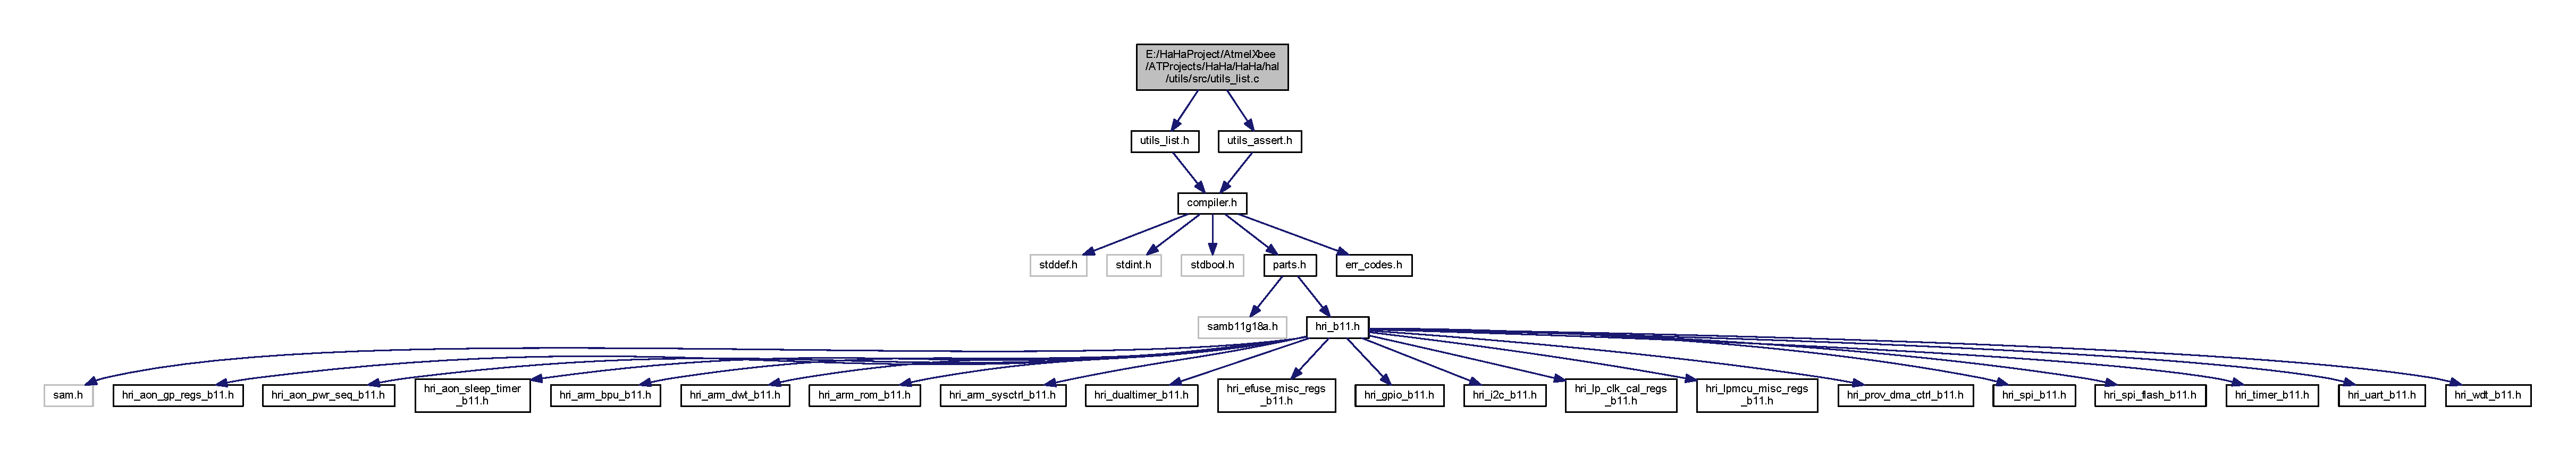
\includegraphics[width=350pt]{utils__list_8c__incl}
\end{center}
\end{figure}
\subsection*{Functions}
\begin{DoxyCompactItemize}
\item 
bool \hyperlink{group__doc__driver__hal__utils__list_ga26022c1362f0fa7e17b734262229c1a7}{is\+\_\+list\+\_\+element} (const struct \hyperlink{structlist__descriptor}{list\+\_\+descriptor} $\ast$const list, const void $\ast$const element)
\begin{DoxyCompactList}\small\item\em Check whether element belongs to list. \end{DoxyCompactList}\item 
void \hyperlink{group__doc__driver__hal__utils__list_gafb3237f00dbf55a40075f3a42c49d32a}{list\+\_\+insert\+\_\+as\+\_\+head} (struct \hyperlink{structlist__descriptor}{list\+\_\+descriptor} $\ast$const list, void $\ast$const element)
\begin{DoxyCompactList}\small\item\em Insert an element as list head. \end{DoxyCompactList}\item 
void \hyperlink{group__doc__driver__hal__utils__list_ga55b8c083fa131f829b1c998e14352f34}{list\+\_\+insert\+\_\+after} (void $\ast$const after, void $\ast$const element)
\begin{DoxyCompactList}\small\item\em Insert an element after the given list element. \end{DoxyCompactList}\item 
void \hyperlink{group__doc__driver__hal__utils__list_ga48c5a1a13223944dd190a6a028075deb}{list\+\_\+insert\+\_\+at\+\_\+end} (struct \hyperlink{structlist__descriptor}{list\+\_\+descriptor} $\ast$const list, void $\ast$const element)
\begin{DoxyCompactList}\small\item\em Insert an element at list end. \end{DoxyCompactList}\item 
void $\ast$ \hyperlink{group__doc__driver__hal__utils__list_ga2269db44f7013963f60c568dd8d08022}{list\+\_\+remove\+\_\+head} (struct \hyperlink{structlist__descriptor}{list\+\_\+descriptor} $\ast$const list)
\begin{DoxyCompactList}\small\item\em Removes list head. \end{DoxyCompactList}\item 
bool \hyperlink{group__doc__driver__hal__utils__list_gad5a2a1ff5dcdfadb47d4ba436e154c98}{list\+\_\+delete\+\_\+element} (struct \hyperlink{structlist__descriptor}{list\+\_\+descriptor} $\ast$const list, const void $\ast$const element)
\begin{DoxyCompactList}\small\item\em Removes list element. \end{DoxyCompactList}\end{DoxyCompactItemize}


\subsection{Detailed Description}
List functionality implementation. 

Copyright (C) 2014 Atmel Corporation. All rights reserved.
\hypertarget{utils__ringbuffer_8c}{}\section{E\+:/\+Ha\+Ha\+Project/\+Atmel\+Xbee/\+A\+T\+Projects/\+Ha\+Ha/\+Ha\+Ha/hal/utils/src/utils\+\_\+ringbuffer.c File Reference}
\label{utils__ringbuffer_8c}\index{E\+:/\+Ha\+Ha\+Project/\+Atmel\+Xbee/\+A\+T\+Projects/\+Ha\+Ha/\+Ha\+Ha/hal/utils/src/utils\+\_\+ringbuffer.\+c@{E\+:/\+Ha\+Ha\+Project/\+Atmel\+Xbee/\+A\+T\+Projects/\+Ha\+Ha/\+Ha\+Ha/hal/utils/src/utils\+\_\+ringbuffer.\+c}}


Ringbuffer functionality implementation.  


{\ttfamily \#include \char`\"{}utils\+\_\+ringbuffer.\+h\char`\"{}}\newline
Include dependency graph for utils\+\_\+ringbuffer.\+c\+:
\nopagebreak
\begin{figure}[H]
\begin{center}
\leavevmode
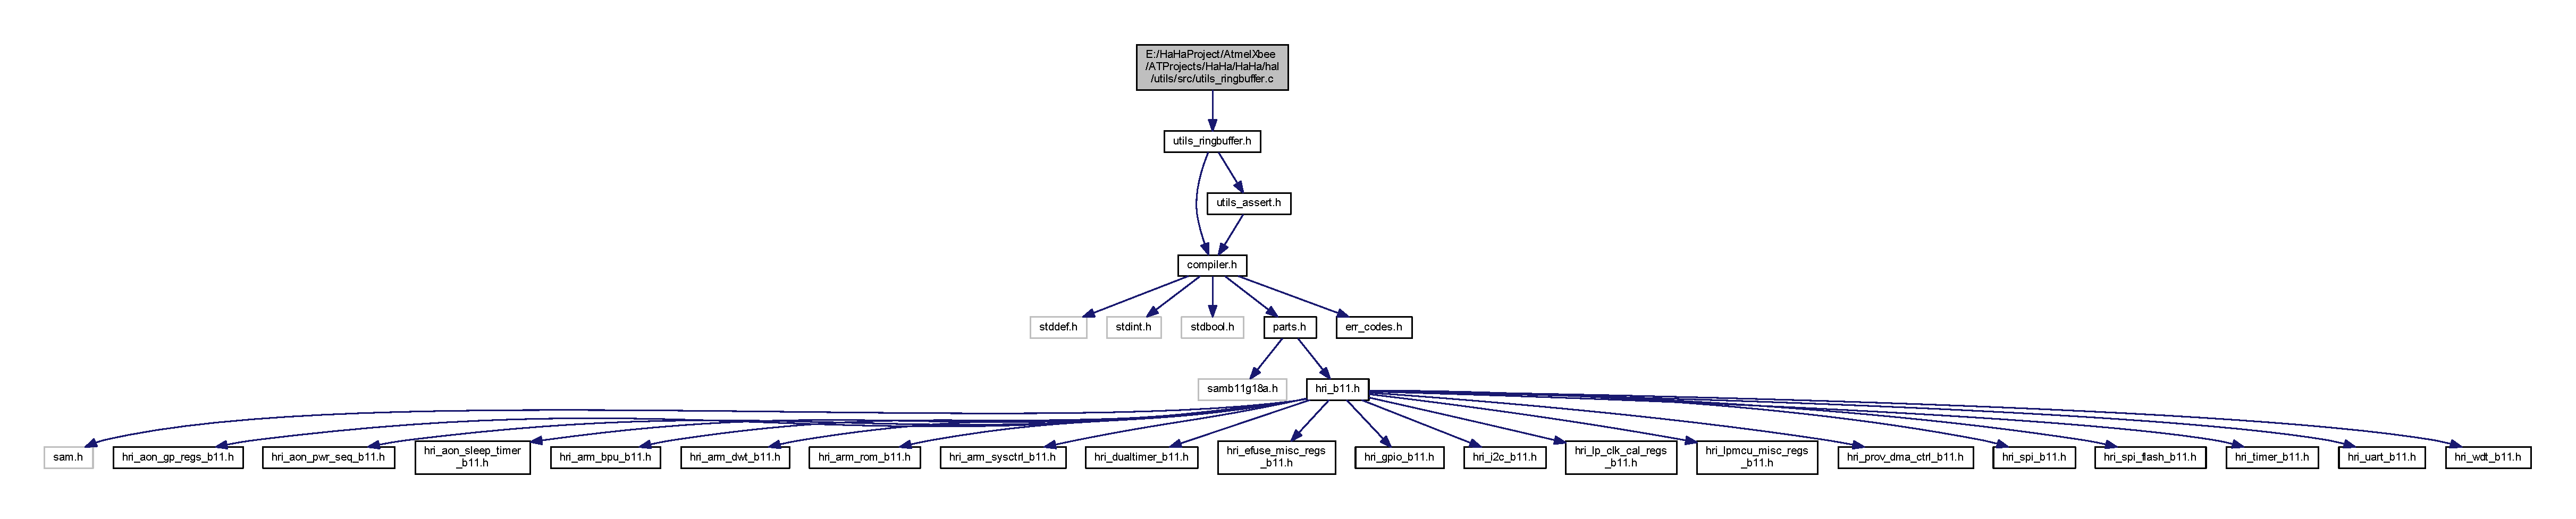
\includegraphics[width=350pt]{utils__ringbuffer_8c__incl}
\end{center}
\end{figure}
\subsection*{Functions}
\begin{DoxyCompactItemize}
\item 
int32\+\_\+t \hyperlink{group__doc__driver__hal__utils__ringbuffer_ga3a02282691d4059ff63caf89b946fbfd}{ringbuffer\+\_\+init} (struct \hyperlink{structringbuffer}{ringbuffer} $\ast$const rb, void $\ast$buf, uint32\+\_\+t size)
\begin{DoxyCompactList}\small\item\em Ringbuffer init. \end{DoxyCompactList}\item 
int32\+\_\+t \hyperlink{group__doc__driver__hal__utils__ringbuffer_ga46163f27edc3b85af50cbc4579e2e8aa}{ringbuffer\+\_\+get} (struct \hyperlink{structringbuffer}{ringbuffer} $\ast$const rb, uint8\+\_\+t $\ast$data)
\begin{DoxyCompactList}\small\item\em Get one byte from ringbuffer. \end{DoxyCompactList}\item 
int32\+\_\+t \hyperlink{group__doc__driver__hal__utils__ringbuffer_ga57c5e4794358ac7f4592fe10c8fccb39}{ringbuffer\+\_\+put} (struct \hyperlink{structringbuffer}{ringbuffer} $\ast$const rb, uint8\+\_\+t data)
\begin{DoxyCompactList}\small\item\em Put one byte to ringbuffer. \end{DoxyCompactList}\item 
uint32\+\_\+t \hyperlink{group__doc__driver__hal__utils__ringbuffer_ga3b4f3772fa2886e7f9429895c1044409}{ringbuffer\+\_\+num} (const struct \hyperlink{structringbuffer}{ringbuffer} $\ast$const rb)
\begin{DoxyCompactList}\small\item\em Return the element number of ringbuffer. \end{DoxyCompactList}\item 
uint32\+\_\+t \hyperlink{group__doc__driver__hal__utils__ringbuffer_ga804ce09a6a02d883da66618ff16cd8f0}{ringbuffer\+\_\+flush} (struct \hyperlink{structringbuffer}{ringbuffer} $\ast$const rb)
\begin{DoxyCompactList}\small\item\em Flush ringbuffer. \end{DoxyCompactList}\end{DoxyCompactItemize}


\subsection{Detailed Description}
Ringbuffer functionality implementation. 

Copyright (C) 2014 Atmel Corporation. All rights reserved.
\hypertarget{utils__syscalls_8c}{}\section{E\+:/\+Ha\+Ha\+Project/\+Atmel\+Xbee/\+A\+T\+Projects/\+Ha\+Ha/\+Ha\+Ha/hal/utils/src/utils\+\_\+syscalls.c File Reference}
\label{utils__syscalls_8c}\index{E\+:/\+Ha\+Ha\+Project/\+Atmel\+Xbee/\+A\+T\+Projects/\+Ha\+Ha/\+Ha\+Ha/hal/utils/src/utils\+\_\+syscalls.\+c@{E\+:/\+Ha\+Ha\+Project/\+Atmel\+Xbee/\+A\+T\+Projects/\+Ha\+Ha/\+Ha\+Ha/hal/utils/src/utils\+\_\+syscalls.\+c}}


Syscalls for S\+A\+M0 (G\+CC).  


{\ttfamily \#include $<$stdio.\+h$>$}\newline
{\ttfamily \#include $<$stdarg.\+h$>$}\newline
{\ttfamily \#include $<$sys/types.\+h$>$}\newline
{\ttfamily \#include $<$sys/stat.\+h$>$}\newline
\subsection*{Functions}
\begin{DoxyCompactItemize}
\item 
\mbox{\Hypertarget{utils__syscalls_8c_aae54d7b9578ba1fc171ce6f30f4c68a3}\label{utils__syscalls_8c_aae54d7b9578ba1fc171ce6f30f4c68a3}} 
caddr\+\_\+t \hyperlink{utils__syscalls_8c_aae54d7b9578ba1fc171ce6f30f4c68a3}{\+\_\+sbrk} (int incr)
\begin{DoxyCompactList}\small\item\em Replacement of C library of \+\_\+sbrk. \end{DoxyCompactList}\item 
\mbox{\Hypertarget{utils__syscalls_8c_aa1f9baeed1efaed3c37861c144b6845b}\label{utils__syscalls_8c_aa1f9baeed1efaed3c37861c144b6845b}} 
int \hyperlink{utils__syscalls_8c_aa1f9baeed1efaed3c37861c144b6845b}{link} (char $\ast$old, char $\ast$\+\_\+new)
\begin{DoxyCompactList}\small\item\em Replacement of C library of link. \end{DoxyCompactList}\item 
\mbox{\Hypertarget{utils__syscalls_8c_a5aab5e2acfd600e3667dc915a2bbc7cb}\label{utils__syscalls_8c_a5aab5e2acfd600e3667dc915a2bbc7cb}} 
int \hyperlink{utils__syscalls_8c_a5aab5e2acfd600e3667dc915a2bbc7cb}{\+\_\+close} (int file)
\begin{DoxyCompactList}\small\item\em Replacement of C library of \+\_\+close. \end{DoxyCompactList}\item 
\mbox{\Hypertarget{utils__syscalls_8c_a41eef54307912a82d20e71c3d47315aa}\label{utils__syscalls_8c_a41eef54307912a82d20e71c3d47315aa}} 
int \hyperlink{utils__syscalls_8c_a41eef54307912a82d20e71c3d47315aa}{\+\_\+fstat} (int file, struct stat $\ast$st)
\begin{DoxyCompactList}\small\item\em Replacement of C library of \+\_\+fstat. \end{DoxyCompactList}\item 
\mbox{\Hypertarget{utils__syscalls_8c_ad3134a3dc296622b8d1c5456e481505b}\label{utils__syscalls_8c_ad3134a3dc296622b8d1c5456e481505b}} 
int \hyperlink{utils__syscalls_8c_ad3134a3dc296622b8d1c5456e481505b}{\+\_\+isatty} (int file)
\begin{DoxyCompactList}\small\item\em Replacement of C library of \+\_\+isatty. \end{DoxyCompactList}\item 
\mbox{\Hypertarget{utils__syscalls_8c_a7a61311bdf1cb025fc07dc2bdae22ce4}\label{utils__syscalls_8c_a7a61311bdf1cb025fc07dc2bdae22ce4}} 
int \hyperlink{utils__syscalls_8c_a7a61311bdf1cb025fc07dc2bdae22ce4}{\+\_\+lseek} (int file, int ptr, int dir)
\begin{DoxyCompactList}\small\item\em Replacement of C library of \+\_\+lseek. \end{DoxyCompactList}\item 
\mbox{\Hypertarget{utils__syscalls_8c_abc96bd69b58b2deaddb484478d911c1b}\label{utils__syscalls_8c_abc96bd69b58b2deaddb484478d911c1b}} 
void \hyperlink{utils__syscalls_8c_abc96bd69b58b2deaddb484478d911c1b}{\+\_\+exit} (int status)
\begin{DoxyCompactList}\small\item\em Replacement of C library of \+\_\+exit. \end{DoxyCompactList}\item 
\mbox{\Hypertarget{utils__syscalls_8c_a3ada001944b574974184d2377be0bec3}\label{utils__syscalls_8c_a3ada001944b574974184d2377be0bec3}} 
void \hyperlink{utils__syscalls_8c_a3ada001944b574974184d2377be0bec3}{\+\_\+kill} (int pid, int sig)
\begin{DoxyCompactList}\small\item\em Replacement of C library of \+\_\+kill. \end{DoxyCompactList}\item 
\mbox{\Hypertarget{utils__syscalls_8c_a945e539df8e0f66d3c73c533fe1968ee}\label{utils__syscalls_8c_a945e539df8e0f66d3c73c533fe1968ee}} 
int \hyperlink{utils__syscalls_8c_a945e539df8e0f66d3c73c533fe1968ee}{\+\_\+getpid} (void)
\begin{DoxyCompactList}\small\item\em Replacement of C library of \+\_\+getpid. \end{DoxyCompactList}\end{DoxyCompactItemize}
\subsection*{Variables}
\begin{DoxyCompactItemize}
\item 
\mbox{\Hypertarget{utils__syscalls_8c_ad65a8842cc674e3ddf69355898c0ecbf}\label{utils__syscalls_8c_ad65a8842cc674e3ddf69355898c0ecbf}} 
int {\bfseries errno}
\item 
\mbox{\Hypertarget{utils__syscalls_8c_abb406f6b7d63af84fda76dbcdbac66c5}\label{utils__syscalls_8c_abb406f6b7d63af84fda76dbcdbac66c5}} 
int {\bfseries \+\_\+end}
\end{DoxyCompactItemize}


\subsection{Detailed Description}
Syscalls for S\+A\+M0 (G\+CC). 

Copyright (C) 2015-\/2016 Atmel Corporation. All rights reserved.
\hypertarget{hpl__core__m0__base_8c}{}\section{E\+:/\+Ha\+Ha\+Project/\+Atmel\+Xbee/\+A\+T\+Projects/\+Ha\+Ha/\+Ha\+Ha/hpl/core/hpl\+\_\+core\+\_\+m0\+\_\+base.c File Reference}
\label{hpl__core__m0__base_8c}\index{E\+:/\+Ha\+Ha\+Project/\+Atmel\+Xbee/\+A\+T\+Projects/\+Ha\+Ha/\+Ha\+Ha/hpl/core/hpl\+\_\+core\+\_\+m0\+\_\+base.\+c@{E\+:/\+Ha\+Ha\+Project/\+Atmel\+Xbee/\+A\+T\+Projects/\+Ha\+Ha/\+Ha\+Ha/hpl/core/hpl\+\_\+core\+\_\+m0\+\_\+base.\+c}}


Core related functionality implementation.  


{\ttfamily \#include $<$hpl\+\_\+core.\+h$>$}\newline
{\ttfamily \#include $<$hpl\+\_\+irq.\+h$>$}\newline
{\ttfamily \#include $<$utils.\+h$>$}\newline
{\ttfamily \#include $<$utils\+\_\+assert.\+h$>$}\newline
\subsection*{Functions}
\begin{DoxyCompactItemize}
\item 
\mbox{\Hypertarget{hpl__core__m0__base_8c_af1c17c7797e22fd860d303deda80e17c}\label{hpl__core__m0__base_8c_af1c17c7797e22fd860d303deda80e17c}} 
void \hyperlink{hpl__core__m0__base_8c_af1c17c7797e22fd860d303deda80e17c}{\+\_\+reset\+\_\+mcu} (void)
\begin{DoxyCompactList}\small\item\em Reset M\+CU. \end{DoxyCompactList}\item 
uint8\+\_\+t \hyperlink{group___h_p_l_ga082e8d19d78ab2cf2f63ded8530c7852}{\+\_\+irq\+\_\+get\+\_\+current} (void)
\begin{DoxyCompactList}\small\item\em Retrieve current I\+RQ number. \end{DoxyCompactList}\item 
void \hyperlink{group___h_p_l_gae6a80cff8a450795dc3f2d6df1a19464}{\+\_\+irq\+\_\+disable} (uint8\+\_\+t n)
\begin{DoxyCompactList}\small\item\em Disable the given I\+RQ. \end{DoxyCompactList}\item 
void \hyperlink{group___h_p_l_ga7720726f19dfdda1561a042483c97a58}{\+\_\+irq\+\_\+set} (uint8\+\_\+t n)
\begin{DoxyCompactList}\small\item\em Set the given I\+RQ. \end{DoxyCompactList}\item 
void \hyperlink{group___h_p_l_ga80f1b1a044a8773e23b38517296620b4}{\+\_\+irq\+\_\+clear} (uint8\+\_\+t n)
\begin{DoxyCompactList}\small\item\em Clear the given I\+RQ. \end{DoxyCompactList}\item 
void \hyperlink{group___h_p_l_gac8b7aa49ad81aecd34603b4dc23dd143}{\+\_\+irq\+\_\+enable} (uint8\+\_\+t n)
\begin{DoxyCompactList}\small\item\em Enable the given I\+RQ. \end{DoxyCompactList}\item 
void \hyperlink{group___h_p_l_ga1ee85f2f8227e335c654b9085e9b7d5c}{\+\_\+irq\+\_\+register} (const uint8\+\_\+t n, struct \hyperlink{struct__irq__descriptor}{\+\_\+irq\+\_\+descriptor} $\ast$const irq)
\begin{DoxyCompactList}\small\item\em Register I\+RQ handler. \end{DoxyCompactList}\item 
\mbox{\Hypertarget{hpl__core__m0__base_8c_a4e0c522c1bb26af24accaf20e6b87d12}\label{hpl__core__m0__base_8c_a4e0c522c1bb26af24accaf20e6b87d12}} 
void \hyperlink{hpl__core__m0__base_8c_a4e0c522c1bb26af24accaf20e6b87d12}{Default\+\_\+\+Handler} (void)
\begin{DoxyCompactList}\small\item\em Default interrupt handler for unused I\+R\+Qs. \end{DoxyCompactList}\end{DoxyCompactItemize}
\subsection*{Variables}
\begin{DoxyCompactItemize}
\item 
\mbox{\Hypertarget{hpl__core__m0__base_8c_a7f41f9238e734e44845a3dc9c71d62d2}\label{hpl__core__m0__base_8c_a7f41f9238e734e44845a3dc9c71d62d2}} 
struct \hyperlink{struct__irq__descriptor}{\+\_\+irq\+\_\+descriptor} $\ast$ \hyperlink{hpl__core__m0__base_8c_a7f41f9238e734e44845a3dc9c71d62d2}{\+\_\+irq\+\_\+table} \mbox{[}P\+E\+R\+I\+P\+H\+\_\+\+C\+O\+U\+N\+T\+\_\+\+I\+R\+Qn\mbox{]}
\begin{DoxyCompactList}\small\item\em The array of interrupt handlers. \end{DoxyCompactList}\end{DoxyCompactItemize}


\subsection{Detailed Description}
Core related functionality implementation. 

Copyright (C) 2016 Atmel Corporation. All rights reserved.
\hypertarget{hpl__core__port_8h}{}\section{E\+:/\+Ha\+Ha\+Project/\+Atmel\+Xbee/\+A\+T\+Projects/\+Ha\+Ha/\+Ha\+Ha/hpl/core/hpl\+\_\+core\+\_\+port.h File Reference}
\label{hpl__core__port_8h}\index{E\+:/\+Ha\+Ha\+Project/\+Atmel\+Xbee/\+A\+T\+Projects/\+Ha\+Ha/\+Ha\+Ha/hpl/core/hpl\+\_\+core\+\_\+port.\+h@{E\+:/\+Ha\+Ha\+Project/\+Atmel\+Xbee/\+A\+T\+Projects/\+Ha\+Ha/\+Ha\+Ha/hpl/core/hpl\+\_\+core\+\_\+port.\+h}}


Core related functionality implementation.  


{\ttfamily \#include $<$peripheral\+\_\+clk\+\_\+config.\+h$>$}\newline
{\ttfamily \#include $<$compiler.\+h$>$}\newline
Include dependency graph for hpl\+\_\+core\+\_\+port.\+h\+:
\nopagebreak
\begin{figure}[H]
\begin{center}
\leavevmode
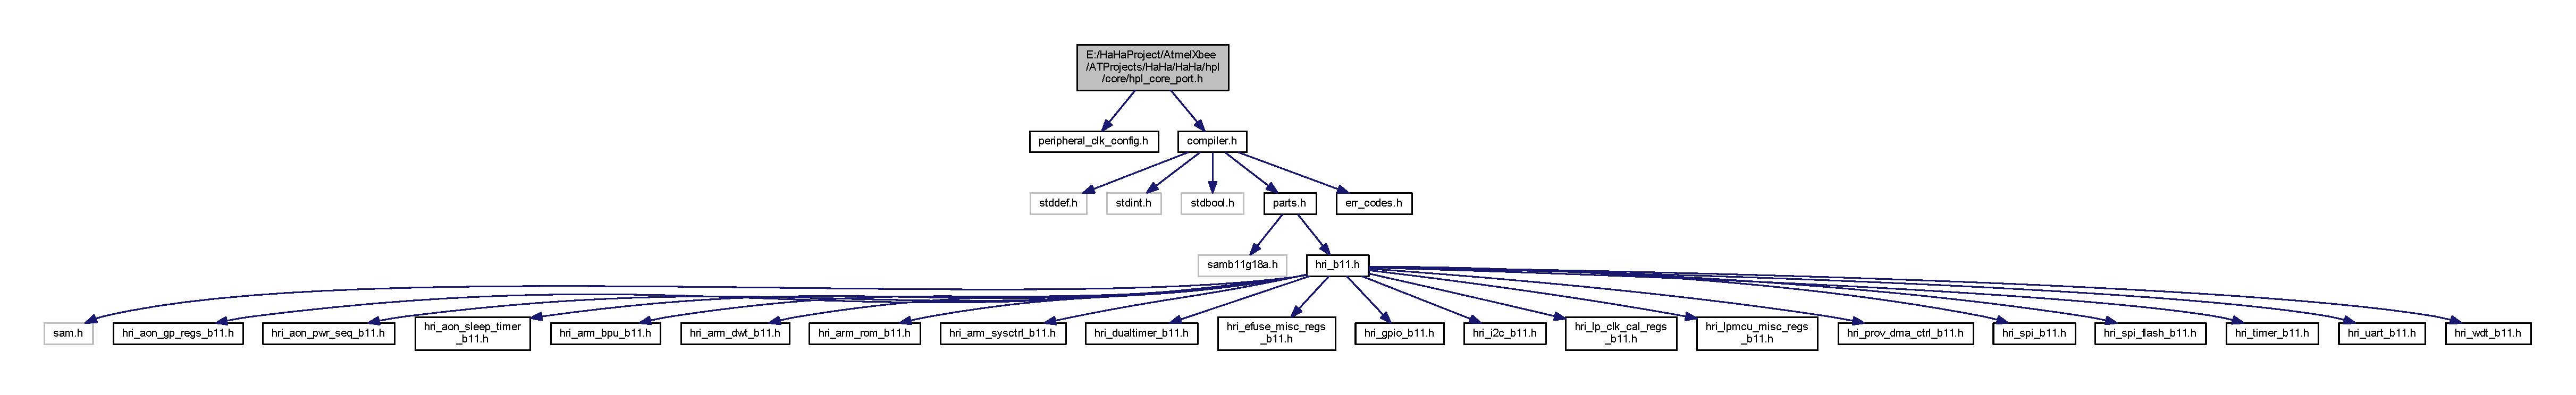
\includegraphics[width=350pt]{hpl__core__port_8h__incl}
\end{center}
\end{figure}
This graph shows which files directly or indirectly include this file\+:
\nopagebreak
\begin{figure}[H]
\begin{center}
\leavevmode
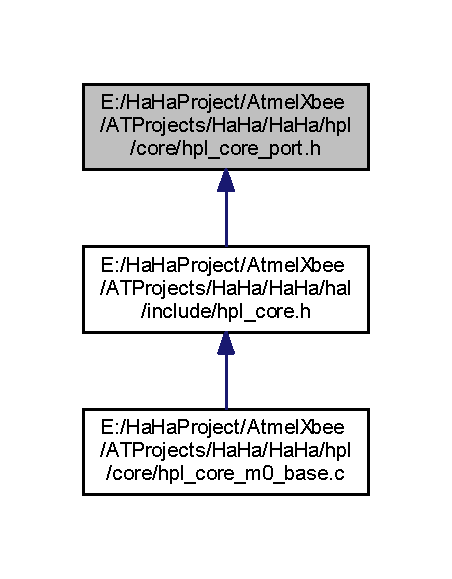
\includegraphics[width=217pt]{hpl__core__port_8h__dep__incl}
\end{center}
\end{figure}


\subsection{Detailed Description}
Core related functionality implementation. 

Copyright (C) 2015 Atmel Corporation. All rights reserved.
\hypertarget{hpl__init_8c}{}\section{E\+:/\+Ha\+Ha\+Project/\+Atmel\+Xbee/\+A\+T\+Projects/\+Ha\+Ha/\+Ha\+Ha/hpl/core/hpl\+\_\+init.c File Reference}
\label{hpl__init_8c}\index{E\+:/\+Ha\+Ha\+Project/\+Atmel\+Xbee/\+A\+T\+Projects/\+Ha\+Ha/\+Ha\+Ha/hpl/core/hpl\+\_\+init.\+c@{E\+:/\+Ha\+Ha\+Project/\+Atmel\+Xbee/\+A\+T\+Projects/\+Ha\+Ha/\+Ha\+Ha/hpl/core/hpl\+\_\+init.\+c}}


H\+PL initialization related functionality implementation.  


{\ttfamily \#include $<$hpl\+\_\+gpio.\+h$>$}\newline
{\ttfamily \#include $<$hpl\+\_\+init.\+h$>$}\newline
\subsection*{Functions}
\begin{DoxyCompactItemize}
\item 
void \hyperlink{group___h_p_l_gac10942d1aec3f0ce14117119db5e9555}{\+\_\+init\+\_\+chip} (void)
\begin{DoxyCompactList}\small\item\em Initialize the hardware abstraction layer. \end{DoxyCompactList}\end{DoxyCompactItemize}


\subsection{Detailed Description}
H\+PL initialization related functionality implementation. 

Copyright (C) 2014-\/2016 Atmel Corporation. All rights reserved.
\hypertarget{hpl__gpio_8c}{}\section{E\+:/\+Ha\+Ha\+Project/\+Atmel\+Xbee/\+A\+T\+Projects/\+Ha\+Ha/\+Ha\+Ha/hpl/gpio/hpl\+\_\+gpio.c File Reference}
\label{hpl__gpio_8c}\index{E\+:/\+Ha\+Ha\+Project/\+Atmel\+Xbee/\+A\+T\+Projects/\+Ha\+Ha/\+Ha\+Ha/hpl/gpio/hpl\+\_\+gpio.\+c@{E\+:/\+Ha\+Ha\+Project/\+Atmel\+Xbee/\+A\+T\+Projects/\+Ha\+Ha/\+Ha\+Ha/hpl/gpio/hpl\+\_\+gpio.\+c}}


S\+AM G\+P\+IO.  


{\ttfamily \#include $<$hpl\+\_\+gpio.\+h$>$}\newline
{\ttfamily \#include $<$utils\+\_\+assert.\+h$>$}\newline
Include dependency graph for hpl\+\_\+gpio.\+c\+:
\nopagebreak
\begin{figure}[H]
\begin{center}
\leavevmode
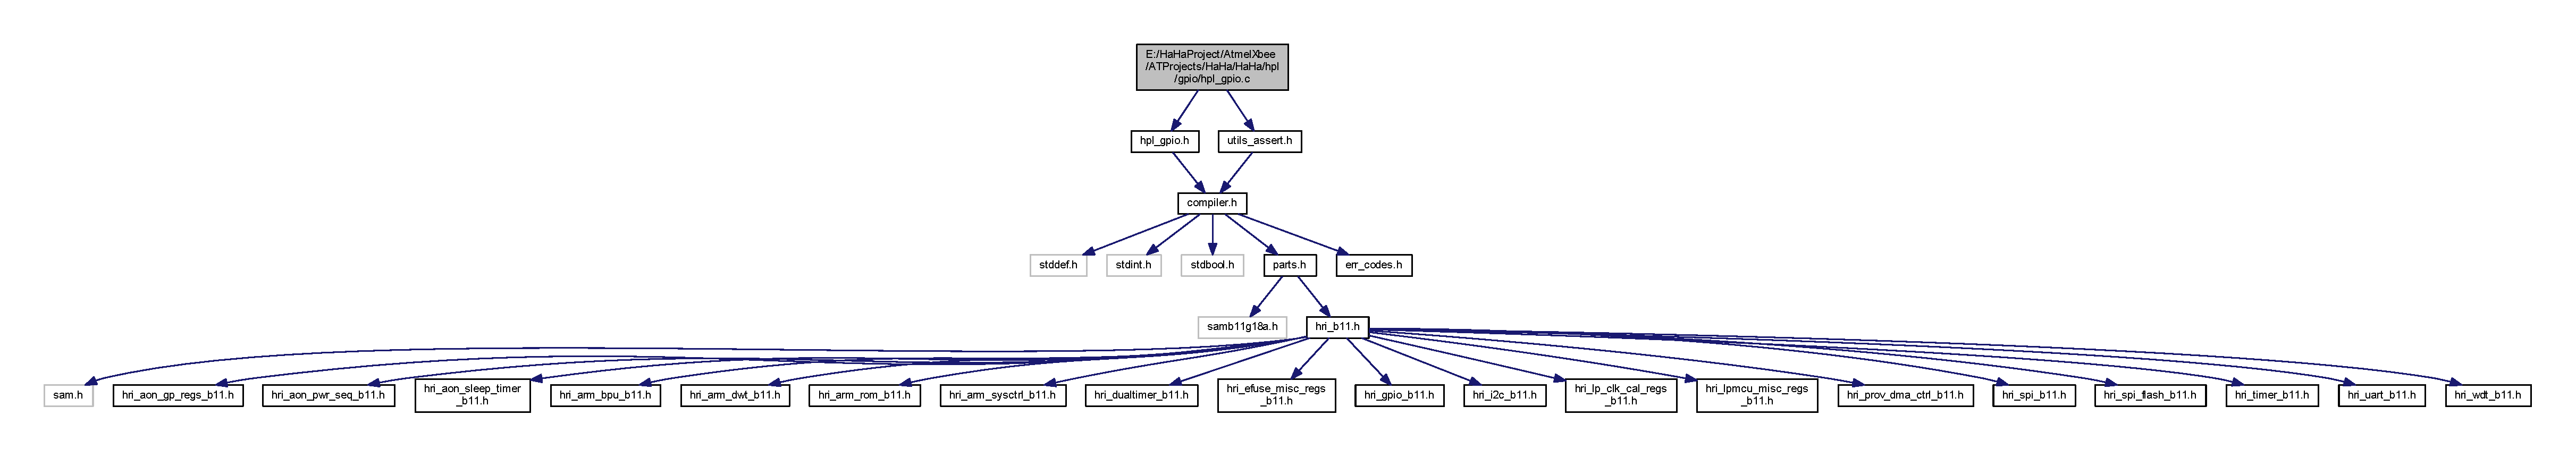
\includegraphics[width=350pt]{hpl__gpio_8c__incl}
\end{center}
\end{figure}
\subsection*{Functions}
\begin{DoxyCompactItemize}
\item 
void \hyperlink{group___h_p_l_gad0c9a05c8d3510204e45f6c292e39996}{\+\_\+gpio\+\_\+set\+\_\+direction} (const enum \hyperlink{group___h_p_l_ga6d50d8c4b17ff573c07340d4d7965bc1}{gpio\+\_\+port} port, const uint32\+\_\+t mask, const enum \hyperlink{group___h_p_l_gaccc7d029df9e5a96151a68e64f4be7e2}{gpio\+\_\+direction} direction)
\begin{DoxyCompactList}\small\item\em Set direction on port with mask. \end{DoxyCompactList}\item 
void \hyperlink{group___h_p_l_ga6dfca37dc99595ea4b013a931a35ba7f}{\+\_\+gpio\+\_\+set\+\_\+level} (const enum \hyperlink{group___h_p_l_ga6d50d8c4b17ff573c07340d4d7965bc1}{gpio\+\_\+port} port, const uint32\+\_\+t mask, const bool level)
\begin{DoxyCompactList}\small\item\em Set output level on port with mask. \end{DoxyCompactList}\item 
void \hyperlink{group___h_p_l_ga00df21e108dc46a00f686923d5cd731e}{\+\_\+gpio\+\_\+toggle\+\_\+level} (const enum \hyperlink{group___h_p_l_ga6d50d8c4b17ff573c07340d4d7965bc1}{gpio\+\_\+port} port, const uint32\+\_\+t mask)
\begin{DoxyCompactList}\small\item\em Change output level to the opposite with mask. \end{DoxyCompactList}\item 
uint32\+\_\+t \hyperlink{group___h_p_l_gaaa9499706a1ad34050473faacabc89af}{\+\_\+gpio\+\_\+get\+\_\+level} (const enum \hyperlink{group___h_p_l_ga6d50d8c4b17ff573c07340d4d7965bc1}{gpio\+\_\+port} port)
\begin{DoxyCompactList}\small\item\em Get input levels on all port pins. \end{DoxyCompactList}\item 
void \hyperlink{group___h_p_l_gaa1ce064a63a47651bbb5a0de9faacc86}{\+\_\+gpio\+\_\+set\+\_\+pin\+\_\+pull\+\_\+mode} (const enum \hyperlink{group___h_p_l_ga6d50d8c4b17ff573c07340d4d7965bc1}{gpio\+\_\+port} port, const uint8\+\_\+t pin, const enum \hyperlink{group___h_p_l_gab9959d4bcdc5049e5898d5100ada3197}{gpio\+\_\+pull\+\_\+mode} pull\+\_\+mode)
\begin{DoxyCompactList}\small\item\em Set pin pull mode. \end{DoxyCompactList}\item 
void \hyperlink{group___h_p_l_gac04d9d84160742c076ff2c1063655cee}{\+\_\+gpio\+\_\+set\+\_\+pin\+\_\+function} (const uint32\+\_\+t gpio, const uint32\+\_\+t function)
\begin{DoxyCompactList}\small\item\em Set pin mux position. \end{DoxyCompactList}\end{DoxyCompactItemize}


\subsection{Detailed Description}
S\+AM G\+P\+IO. 

Copyright (C) 2015-\/2016 Atmel Corporation. All rights reserved.
\hypertarget{hpl__lpmcu__misc__regs_8c}{}\section{E\+:/\+Ha\+Ha\+Project/\+Atmel\+Xbee/\+A\+T\+Projects/\+Ha\+Ha/\+Ha\+Ha/hpl/lpmcu\+\_\+misc\+\_\+regs/hpl\+\_\+lpmcu\+\_\+misc\+\_\+regs.c File Reference}
\label{hpl__lpmcu__misc__regs_8c}\index{E\+:/\+Ha\+Ha\+Project/\+Atmel\+Xbee/\+A\+T\+Projects/\+Ha\+Ha/\+Ha\+Ha/hpl/lpmcu\+\_\+misc\+\_\+regs/hpl\+\_\+lpmcu\+\_\+misc\+\_\+regs.\+c@{E\+:/\+Ha\+Ha\+Project/\+Atmel\+Xbee/\+A\+T\+Projects/\+Ha\+Ha/\+Ha\+Ha/hpl/lpmcu\+\_\+misc\+\_\+regs/hpl\+\_\+lpmcu\+\_\+misc\+\_\+regs.\+c}}


Low power M\+CU misc register v100 related functionality.  


{\ttfamily \#include $<$hpl\+\_\+lpmcu\+\_\+misc\+\_\+regs\+\_\+config.\+h$>$}\newline
{\ttfamily \#include $<$hpl\+\_\+init.\+h$>$}\newline
Include dependency graph for hpl\+\_\+lpmcu\+\_\+misc\+\_\+regs.\+c\+:\nopagebreak
\begin{figure}[H]
\begin{center}
\leavevmode
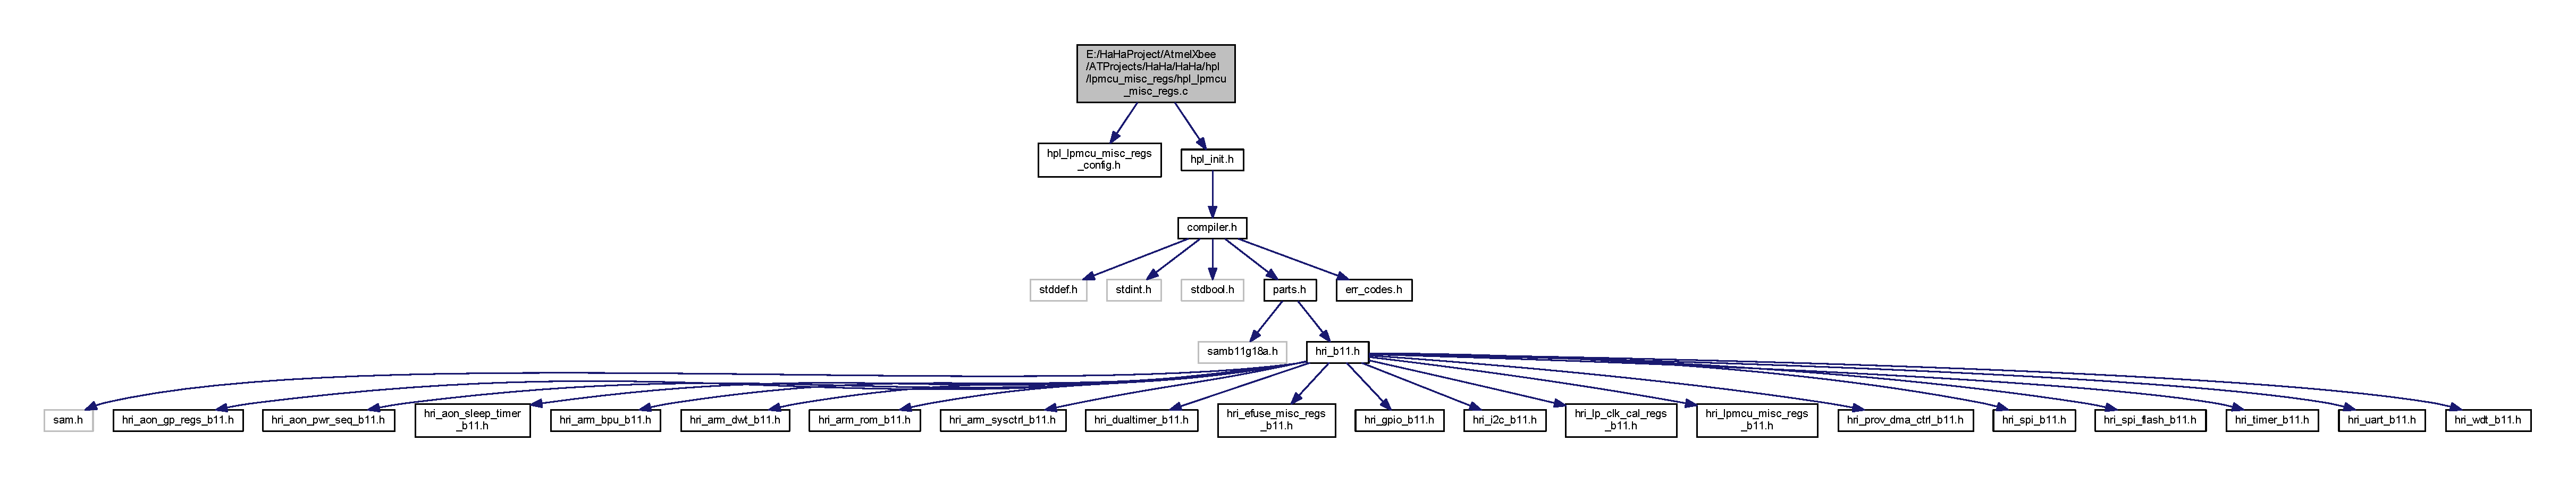
\includegraphics[width=350pt]{hpl__lpmcu__misc__regs_8c__incl}
\end{center}
\end{figure}
\subsection*{Functions}
\begin{DoxyCompactItemize}
\item 
void \hyperlink{group___h_p_l_ga3dd85007c9fdeed2ffe1166a33dd6519}{\+\_\+lpmcu\+\_\+misc\+\_\+regs\+\_\+init} (void)
\begin{DoxyCompactList}\small\item\em Initializes cortex M0 core clock. \end{DoxyCompactList}\end{DoxyCompactItemize}


\subsection{Detailed Description}
Low power M\+CU misc register v100 related functionality. 

Copyright (C) 2015 Atmel Corporation. All rights reserved.
\hypertarget{hpl__uart_8c}{}\section{E\+:/\+Ha\+Ha\+Project/\+Atmel\+Xbee/\+A\+T\+Projects/\+Ha\+Ha/\+Ha\+Ha/hpl/uart/hpl\+\_\+uart.c File Reference}
\label{hpl__uart_8c}\index{E\+:/\+Ha\+Ha\+Project/\+Atmel\+Xbee/\+A\+T\+Projects/\+Ha\+Ha/\+Ha\+Ha/hpl/uart/hpl\+\_\+uart.\+c@{E\+:/\+Ha\+Ha\+Project/\+Atmel\+Xbee/\+A\+T\+Projects/\+Ha\+Ha/\+Ha\+Ha/hpl/uart/hpl\+\_\+uart.\+c}}


S\+AM Serial Communication Interface.  


{\ttfamily \#include $<$utils\+\_\+assert.\+h$>$}\newline
{\ttfamily \#include $<$utils.\+h$>$}\newline
{\ttfamily \#include $<$hpl\+\_\+usart\+\_\+async.\+h$>$}\newline
{\ttfamily \#include $<$hpl\+\_\+usart\+\_\+sync.\+h$>$}\newline
{\ttfamily \#include $<$hpl\+\_\+uart\+\_\+config.\+h$>$}\newline
Include dependency graph for hpl\+\_\+uart.\+c\+:\nopagebreak
\begin{figure}[H]
\begin{center}
\leavevmode
\includegraphics[width=350pt]{hpl__uart_8c__incl}
\end{center}
\end{figure}
\subsection*{Classes}
\begin{DoxyCompactItemize}
\item 
struct \hyperlink{structuart__config}{uart\+\_\+config}
\begin{DoxyCompactList}\small\item\em Configuration structure for the U\+A\+RT module. \end{DoxyCompactList}\end{DoxyCompactItemize}
\subsection*{Macros}
\begin{DoxyCompactItemize}
\item 
\#define \hyperlink{hpl__uart_8c_ad97f1728892384250c4f93b4b4706e40}{C\+O\+N\+F\+\_\+\+U\+A\+R\+T\+\_\+0\+\_\+\+E\+N\+A\+B\+LE}~0
\item 
\#define \hyperlink{hpl__uart_8c_acbc19956936bba02e5387c2debd6aad5}{C\+O\+N\+F\+\_\+\+U\+A\+R\+T\+\_\+1\+\_\+\+E\+N\+A\+B\+LE}~0
\item 
\#define \hyperlink{hpl__uart_8c_a5e9bdee638cdfc768258e0155df437fc}{U\+A\+R\+T\+\_\+\+A\+M\+O\+U\+NT}~(\hyperlink{hpl__uart_8c_ad97f1728892384250c4f93b4b4706e40}{C\+O\+N\+F\+\_\+\+U\+A\+R\+T\+\_\+0\+\_\+\+E\+N\+A\+B\+LE} + \hyperlink{hpl__uart_8c_acbc19956936bba02e5387c2debd6aad5}{C\+O\+N\+F\+\_\+\+U\+A\+R\+T\+\_\+1\+\_\+\+E\+N\+A\+B\+LE})
\item 
\#define \hyperlink{hpl__uart_8c_a53b06f9eff53ee8bca1d489cc7be7597}{U\+A\+R\+T\+\_\+\+C\+O\+N\+F\+I\+G\+U\+R\+A\+T\+I\+ON}(n)
\begin{DoxyCompactList}\small\item\em Macro is used to fill U\+A\+RT configuration structure based on its number. \end{DoxyCompactList}\end{DoxyCompactItemize}
\subsection*{Functions}
\begin{DoxyCompactItemize}
\item 
void \hyperlink{hpl__uart_8c_a8192d7f8c9770ce1683f341ba467a66e}{U\+A\+R\+T1\+\_\+\+R\+X\+\_\+\+Handler} (void)
\item 
void \hyperlink{hpl__uart_8c_a627ce7fd62cdd9e05ee5f3512dfed181}{U\+A\+R\+T1\+\_\+\+T\+X\+\_\+\+Handler} (void)
\item 
int32\+\_\+t \hyperlink{group___h_p_l_gad1cc7b8e72fd67fdeec8062c802eb25a}{\+\_\+usart\+\_\+sync\+\_\+init} (struct \hyperlink{struct__usart__sync__device}{\+\_\+usart\+\_\+sync\+\_\+device} $\ast$const device, void $\ast$const hw)
\begin{DoxyCompactList}\small\item\em Initialize synchronous U\+A\+RT. \end{DoxyCompactList}\item 
int32\+\_\+t \hyperlink{group___h_p_l_ga11745e0bd0c9d636afbefae8e209665e}{\+\_\+usart\+\_\+async\+\_\+init} (struct \hyperlink{struct__usart__async__device}{\+\_\+usart\+\_\+async\+\_\+device} $\ast$const device, void $\ast$const hw)
\begin{DoxyCompactList}\small\item\em Initialize asynchronous U\+A\+RT. \end{DoxyCompactList}\item 
void \hyperlink{group___h_p_l_gac046761a56aaedeba5acad135cab707c}{\+\_\+usart\+\_\+sync\+\_\+deinit} (struct \hyperlink{struct__usart__sync__device}{\+\_\+usart\+\_\+sync\+\_\+device} $\ast$const device)
\begin{DoxyCompactList}\small\item\em De-\/initialize U\+A\+RT. \end{DoxyCompactList}\item 
void \hyperlink{group___h_p_l_ga57e2ef9f6ec11c53a9d88bdb7a82aac4}{\+\_\+usart\+\_\+async\+\_\+deinit} (struct \hyperlink{struct__usart__async__device}{\+\_\+usart\+\_\+async\+\_\+device} $\ast$const device)
\begin{DoxyCompactList}\small\item\em De-\/initialize U\+A\+RT. \end{DoxyCompactList}\item 
void \hyperlink{group___h_p_l_ga5ca07057bde212b46f6547e5bdb876de}{\+\_\+usart\+\_\+sync\+\_\+enable} (struct \hyperlink{struct__usart__sync__device}{\+\_\+usart\+\_\+sync\+\_\+device} $\ast$const device)
\begin{DoxyCompactList}\small\item\em Enable U\+A\+RT module. \end{DoxyCompactList}\item 
void \hyperlink{group___h_p_l_ga86c4101798d9dbc584f1e56615140d6f}{\+\_\+usart\+\_\+async\+\_\+enable} (struct \hyperlink{struct__usart__async__device}{\+\_\+usart\+\_\+async\+\_\+device} $\ast$const device)
\begin{DoxyCompactList}\small\item\em Enable U\+A\+RT module. \end{DoxyCompactList}\item 
void \hyperlink{group___h_p_l_gac021f29c77d8a9bfabfdd7433dbbb024}{\+\_\+usart\+\_\+sync\+\_\+disable} (struct \hyperlink{struct__usart__sync__device}{\+\_\+usart\+\_\+sync\+\_\+device} $\ast$const device)
\begin{DoxyCompactList}\small\item\em Disable U\+A\+RT module. \end{DoxyCompactList}\item 
void \hyperlink{group___h_p_l_gadb6751e5c270eb88eb754f45e7b8a91f}{\+\_\+usart\+\_\+async\+\_\+disable} (struct \hyperlink{struct__usart__async__device}{\+\_\+usart\+\_\+async\+\_\+device} $\ast$const device)
\begin{DoxyCompactList}\small\item\em Disable U\+A\+RT module. \end{DoxyCompactList}\item 
void \hyperlink{group___h_p_l_ga882c8cecf50eb1276401d6874956b903}{\+\_\+usart\+\_\+sync\+\_\+set\+\_\+baud\+\_\+rate} (struct \hyperlink{struct__usart__sync__device}{\+\_\+usart\+\_\+sync\+\_\+device} $\ast$const device, const uint32\+\_\+t baud\+\_\+rate)
\begin{DoxyCompactList}\small\item\em Set baud rate. \end{DoxyCompactList}\item 
void \hyperlink{group___h_p_l_gab3211a57f9d6f2e355db5b67ce3fe905}{\+\_\+usart\+\_\+async\+\_\+set\+\_\+baud\+\_\+rate} (struct \hyperlink{struct__usart__async__device}{\+\_\+usart\+\_\+async\+\_\+device} $\ast$const device, const uint32\+\_\+t baud\+\_\+rate)
\begin{DoxyCompactList}\small\item\em Set baud rate. \end{DoxyCompactList}\item 
void \hyperlink{group___h_p_l_ga1b30e54d42d94ab59067e121d286d47a}{\+\_\+usart\+\_\+sync\+\_\+set\+\_\+data\+\_\+order} (struct \hyperlink{struct__usart__sync__device}{\+\_\+usart\+\_\+sync\+\_\+device} $\ast$const device, const enum \hyperlink{group___h_p_l_ga426849bbd9655cec091101ebc9123eb4}{usart\+\_\+data\+\_\+order} order)
\begin{DoxyCompactList}\small\item\em Set data order. \end{DoxyCompactList}\item 
void \hyperlink{group___h_p_l_ga8f29c61bfbc9298ba0e25be2980ddd15}{\+\_\+usart\+\_\+async\+\_\+set\+\_\+data\+\_\+order} (struct \hyperlink{struct__usart__async__device}{\+\_\+usart\+\_\+async\+\_\+device} $\ast$const device, const enum \hyperlink{group___h_p_l_ga426849bbd9655cec091101ebc9123eb4}{usart\+\_\+data\+\_\+order} order)
\begin{DoxyCompactList}\small\item\em Set data order. \end{DoxyCompactList}\item 
void \hyperlink{group___h_p_l_ga2dd82ebe0069e4c61fda94ac0dda1a63}{\+\_\+usart\+\_\+sync\+\_\+set\+\_\+mode} (struct \hyperlink{struct__usart__sync__device}{\+\_\+usart\+\_\+sync\+\_\+device} $\ast$const device, const enum \hyperlink{group___h_p_l_ga1c465965478e0f6908a4c99d4f3ad20f}{usart\+\_\+mode} mode)
\begin{DoxyCompactList}\small\item\em Set mode. \end{DoxyCompactList}\item 
void \hyperlink{group___h_p_l_gaee0a2babdf7b777fa4754028c92fc2e8}{\+\_\+usart\+\_\+sync\+\_\+set\+\_\+parity} (struct \hyperlink{struct__usart__sync__device}{\+\_\+usart\+\_\+sync\+\_\+device} $\ast$const device, const enum \hyperlink{group___h_p_l_ga867cc5f0ea7d3bf651d68f0046cf6f41}{usart\+\_\+parity} parity)
\begin{DoxyCompactList}\small\item\em Set parity. \end{DoxyCompactList}\item 
void \hyperlink{group___h_p_l_ga739cdfde316390a089c38355bc4f596e}{\+\_\+usart\+\_\+async\+\_\+set\+\_\+parity} (struct \hyperlink{struct__usart__async__device}{\+\_\+usart\+\_\+async\+\_\+device} $\ast$const device, const enum \hyperlink{group___h_p_l_ga867cc5f0ea7d3bf651d68f0046cf6f41}{usart\+\_\+parity} parity)
\begin{DoxyCompactList}\small\item\em Set parity. \end{DoxyCompactList}\item 
void \hyperlink{group___h_p_l_ga93c7de4ab355c189e306288d21642ff3}{\+\_\+usart\+\_\+sync\+\_\+set\+\_\+stop\+\_\+bits} (struct \hyperlink{struct__usart__sync__device}{\+\_\+usart\+\_\+sync\+\_\+device} $\ast$const device, const enum \hyperlink{group___h_p_l_ga88311517c5168c29a681604a8a33b06e}{usart\+\_\+stop\+\_\+bits} stop\+\_\+bits)
\begin{DoxyCompactList}\small\item\em Set stop bits mode. \end{DoxyCompactList}\item 
void \hyperlink{group___h_p_l_ga7f2ef73e4b9da5be12fc0eabb97ab67b}{\+\_\+usart\+\_\+async\+\_\+set\+\_\+stop\+\_\+bits} (struct \hyperlink{struct__usart__async__device}{\+\_\+usart\+\_\+async\+\_\+device} $\ast$const device, const enum \hyperlink{group___h_p_l_ga88311517c5168c29a681604a8a33b06e}{usart\+\_\+stop\+\_\+bits} stop\+\_\+bits)
\begin{DoxyCompactList}\small\item\em Set stop bits mode. \end{DoxyCompactList}\item 
void \hyperlink{group___h_p_l_ga45ebffe94571d266e42b3dd882ad559d}{\+\_\+usart\+\_\+sync\+\_\+set\+\_\+character\+\_\+size} (struct \hyperlink{struct__usart__sync__device}{\+\_\+usart\+\_\+sync\+\_\+device} $\ast$const device, const enum \hyperlink{group___h_p_l_ga631ce7b4f60dccd392e6d6ef7d3cd4e2}{usart\+\_\+character\+\_\+size} size)
\begin{DoxyCompactList}\small\item\em Set character size. \end{DoxyCompactList}\item 
void \hyperlink{group___h_p_l_gaf834af5cc0738976ddbc200901aef105}{\+\_\+usart\+\_\+async\+\_\+set\+\_\+character\+\_\+size} (struct \hyperlink{struct__usart__async__device}{\+\_\+usart\+\_\+async\+\_\+device} $\ast$const device, const enum \hyperlink{group___h_p_l_ga631ce7b4f60dccd392e6d6ef7d3cd4e2}{usart\+\_\+character\+\_\+size} size)
\begin{DoxyCompactList}\small\item\em Set character size. \end{DoxyCompactList}\item 
uint32\+\_\+t \hyperlink{group___h_p_l_ga512c769b924d59433542bf347980334b}{\+\_\+usart\+\_\+sync\+\_\+get\+\_\+status} (const struct \hyperlink{struct__usart__sync__device}{\+\_\+usart\+\_\+sync\+\_\+device} $\ast$const device)
\begin{DoxyCompactList}\small\item\em Retrieve uart status. \end{DoxyCompactList}\item 
uint32\+\_\+t \hyperlink{group___h_p_l_ga09d708dc23dacf358d3de8a3a0545c1a}{\+\_\+usart\+\_\+async\+\_\+get\+\_\+status} (const struct \hyperlink{struct__usart__async__device}{\+\_\+usart\+\_\+async\+\_\+device} $\ast$const device)
\begin{DoxyCompactList}\small\item\em Retrieve uart status. \end{DoxyCompactList}\item 
void \hyperlink{group___h_p_l_ga6f9cc0e2020d49845bef97301bc692e0}{\+\_\+usart\+\_\+sync\+\_\+write\+\_\+byte} (struct \hyperlink{struct__usart__sync__device}{\+\_\+usart\+\_\+sync\+\_\+device} $\ast$const device, uint8\+\_\+t data)
\begin{DoxyCompactList}\small\item\em Write a byte to the given U\+A\+RT instance. \end{DoxyCompactList}\item 
void \hyperlink{group___h_p_l_ga3a2887cd1710eaad2df0e66b9e830faa}{\+\_\+usart\+\_\+async\+\_\+write\+\_\+byte} (struct \hyperlink{struct__usart__async__device}{\+\_\+usart\+\_\+async\+\_\+device} $\ast$const device, uint8\+\_\+t data)
\begin{DoxyCompactList}\small\item\em Write a byte to the given U\+A\+RT instance. \end{DoxyCompactList}\item 
uint8\+\_\+t \hyperlink{group___h_p_l_gad6e42aaa92499103016d605362e35d97}{\+\_\+usart\+\_\+sync\+\_\+read\+\_\+byte} (const struct \hyperlink{struct__usart__sync__device}{\+\_\+usart\+\_\+sync\+\_\+device} $\ast$const device)
\begin{DoxyCompactList}\small\item\em Read a byte from the given U\+A\+RT instance. \end{DoxyCompactList}\item 
bool \hyperlink{group___h_p_l_ga8bad9999c03b728f47848b2337393ec4}{\+\_\+usart\+\_\+sync\+\_\+is\+\_\+byte\+\_\+sent} (const struct \hyperlink{struct__usart__sync__device}{\+\_\+usart\+\_\+sync\+\_\+device} $\ast$const device)
\begin{DoxyCompactList}\small\item\em Check if U\+A\+RT is ready to send next byte. \end{DoxyCompactList}\item 
bool \hyperlink{group___h_p_l_gaf96fbe9e0e063f4ae332451b7a540e2c}{\+\_\+usart\+\_\+async\+\_\+is\+\_\+byte\+\_\+sent} (const struct \hyperlink{struct__usart__async__device}{\+\_\+usart\+\_\+async\+\_\+device} $\ast$const device)
\begin{DoxyCompactList}\small\item\em Check if U\+A\+RT is ready to send next byte. \end{DoxyCompactList}\item 
bool \hyperlink{group___h_p_l_ga5bf04a89be94430de57acf53f9b35dd2}{\+\_\+usart\+\_\+sync\+\_\+is\+\_\+byte\+\_\+received} (const struct \hyperlink{struct__usart__sync__device}{\+\_\+usart\+\_\+sync\+\_\+device} $\ast$const device)
\begin{DoxyCompactList}\small\item\em Check if there is data received by U\+A\+RT. \end{DoxyCompactList}\item 
void \hyperlink{group___h_p_l_gae43bb6755eb8c462a9884e6cdca602aa}{\+\_\+usart\+\_\+sync\+\_\+set\+\_\+flow\+\_\+control\+\_\+state} (struct \hyperlink{struct__usart__sync__device}{\+\_\+usart\+\_\+sync\+\_\+device} $\ast$const device, const union \hyperlink{unionusart__flow__control__state}{usart\+\_\+flow\+\_\+control\+\_\+state} state)
\begin{DoxyCompactList}\small\item\em Set the state of flow control pins. \end{DoxyCompactList}\item 
void \hyperlink{group___h_p_l_gafdf581028b78744fccccae79d45a2078}{\+\_\+usart\+\_\+async\+\_\+set\+\_\+flow\+\_\+control\+\_\+state} (struct \hyperlink{struct__usart__async__device}{\+\_\+usart\+\_\+async\+\_\+device} $\ast$const device, const union \hyperlink{unionusart__flow__control__state}{usart\+\_\+flow\+\_\+control\+\_\+state} state)
\begin{DoxyCompactList}\small\item\em Set the state of flow control pins. \end{DoxyCompactList}\item 
union \hyperlink{unionusart__flow__control__state}{usart\+\_\+flow\+\_\+control\+\_\+state} \hyperlink{group___h_p_l_ga5b6662f283d7a2791c7eed77635e9238}{\+\_\+usart\+\_\+sync\+\_\+get\+\_\+flow\+\_\+control\+\_\+state} (const struct \hyperlink{struct__usart__sync__device}{\+\_\+usart\+\_\+sync\+\_\+device} $\ast$const device)
\begin{DoxyCompactList}\small\item\em Retrieve the state of flow control pins. \end{DoxyCompactList}\item 
union \hyperlink{unionusart__flow__control__state}{usart\+\_\+flow\+\_\+control\+\_\+state} \hyperlink{group___h_p_l_gaa9850f9d97cb87f80fa615e95330ce35}{\+\_\+usart\+\_\+async\+\_\+get\+\_\+flow\+\_\+control\+\_\+state} (const struct \hyperlink{struct__usart__async__device}{\+\_\+usart\+\_\+async\+\_\+device} $\ast$const device)
\begin{DoxyCompactList}\small\item\em Retrieve the state of flow control pins. \end{DoxyCompactList}\item 
void \hyperlink{group___h_p_l_ga5dcb14840b2011da3a1d0f774dafa28d}{\+\_\+usart\+\_\+async\+\_\+enable\+\_\+byte\+\_\+sent\+\_\+irq} (struct \hyperlink{struct__usart__async__device}{\+\_\+usart\+\_\+async\+\_\+device} $\ast$const device)
\begin{DoxyCompactList}\small\item\em Enable data register empty interrupt. \end{DoxyCompactList}\item 
void \hyperlink{group___h_p_l_ga89bf3d02a7a3cca261900906ffd9ca76}{\+\_\+usart\+\_\+async\+\_\+enable\+\_\+tx\+\_\+done\+\_\+irq} (struct \hyperlink{struct__usart__async__device}{\+\_\+usart\+\_\+async\+\_\+device} $\ast$const device)
\begin{DoxyCompactList}\small\item\em Enable transmission complete interrupt. \end{DoxyCompactList}\item 
void \hyperlink{group___h_p_l_gadd7a2a78a76c6286f474bdce333c4904}{\+\_\+usart\+\_\+async\+\_\+set\+\_\+irq\+\_\+state} (struct \hyperlink{struct__usart__async__device}{\+\_\+usart\+\_\+async\+\_\+device} $\ast$const device, const enum \hyperlink{group___h_p_l_gace00dc77ac02c91f8bf35551b484927c}{\+\_\+usart\+\_\+async\+\_\+callback\+\_\+type} type, const bool state)
\begin{DoxyCompactList}\small\item\em Enable/disable U\+A\+RT interrupt. \end{DoxyCompactList}\end{DoxyCompactItemize}


\subsection{Detailed Description}
S\+AM Serial Communication Interface. 

Copyright (C) 2016 -\/ 2017 Atmel Corporation. All rights reserved.

\subsection{Macro Definition Documentation}
\mbox{\Hypertarget{hpl__uart_8c_ad97f1728892384250c4f93b4b4706e40}\label{hpl__uart_8c_ad97f1728892384250c4f93b4b4706e40}} 
\index{hpl\+\_\+uart.\+c@{hpl\+\_\+uart.\+c}!C\+O\+N\+F\+\_\+\+U\+A\+R\+T\+\_\+0\+\_\+\+E\+N\+A\+B\+LE@{C\+O\+N\+F\+\_\+\+U\+A\+R\+T\+\_\+0\+\_\+\+E\+N\+A\+B\+LE}}
\index{C\+O\+N\+F\+\_\+\+U\+A\+R\+T\+\_\+0\+\_\+\+E\+N\+A\+B\+LE@{C\+O\+N\+F\+\_\+\+U\+A\+R\+T\+\_\+0\+\_\+\+E\+N\+A\+B\+LE}!hpl\+\_\+uart.\+c@{hpl\+\_\+uart.\+c}}
\subsubsection{\texorpdfstring{C\+O\+N\+F\+\_\+\+U\+A\+R\+T\+\_\+0\+\_\+\+E\+N\+A\+B\+LE}{CONF\_UART\_0\_ENABLE}}
{\footnotesize\ttfamily \#define C\+O\+N\+F\+\_\+\+U\+A\+R\+T\+\_\+0\+\_\+\+E\+N\+A\+B\+LE~0}

\mbox{\Hypertarget{hpl__uart_8c_acbc19956936bba02e5387c2debd6aad5}\label{hpl__uart_8c_acbc19956936bba02e5387c2debd6aad5}} 
\index{hpl\+\_\+uart.\+c@{hpl\+\_\+uart.\+c}!C\+O\+N\+F\+\_\+\+U\+A\+R\+T\+\_\+1\+\_\+\+E\+N\+A\+B\+LE@{C\+O\+N\+F\+\_\+\+U\+A\+R\+T\+\_\+1\+\_\+\+E\+N\+A\+B\+LE}}
\index{C\+O\+N\+F\+\_\+\+U\+A\+R\+T\+\_\+1\+\_\+\+E\+N\+A\+B\+LE@{C\+O\+N\+F\+\_\+\+U\+A\+R\+T\+\_\+1\+\_\+\+E\+N\+A\+B\+LE}!hpl\+\_\+uart.\+c@{hpl\+\_\+uart.\+c}}
\subsubsection{\texorpdfstring{C\+O\+N\+F\+\_\+\+U\+A\+R\+T\+\_\+1\+\_\+\+E\+N\+A\+B\+LE}{CONF\_UART\_1\_ENABLE}}
{\footnotesize\ttfamily \#define C\+O\+N\+F\+\_\+\+U\+A\+R\+T\+\_\+1\+\_\+\+E\+N\+A\+B\+LE~0}

\mbox{\Hypertarget{hpl__uart_8c_a5e9bdee638cdfc768258e0155df437fc}\label{hpl__uart_8c_a5e9bdee638cdfc768258e0155df437fc}} 
\index{hpl\+\_\+uart.\+c@{hpl\+\_\+uart.\+c}!U\+A\+R\+T\+\_\+\+A\+M\+O\+U\+NT@{U\+A\+R\+T\+\_\+\+A\+M\+O\+U\+NT}}
\index{U\+A\+R\+T\+\_\+\+A\+M\+O\+U\+NT@{U\+A\+R\+T\+\_\+\+A\+M\+O\+U\+NT}!hpl\+\_\+uart.\+c@{hpl\+\_\+uart.\+c}}
\subsubsection{\texorpdfstring{U\+A\+R\+T\+\_\+\+A\+M\+O\+U\+NT}{UART\_AMOUNT}}
{\footnotesize\ttfamily \#define U\+A\+R\+T\+\_\+\+A\+M\+O\+U\+NT~(\hyperlink{hpl__uart_8c_ad97f1728892384250c4f93b4b4706e40}{C\+O\+N\+F\+\_\+\+U\+A\+R\+T\+\_\+0\+\_\+\+E\+N\+A\+B\+LE} + \hyperlink{hpl__uart_8c_acbc19956936bba02e5387c2debd6aad5}{C\+O\+N\+F\+\_\+\+U\+A\+R\+T\+\_\+1\+\_\+\+E\+N\+A\+B\+LE})}

Amount of U\+A\+RT. \mbox{\Hypertarget{hpl__uart_8c_a53b06f9eff53ee8bca1d489cc7be7597}\label{hpl__uart_8c_a53b06f9eff53ee8bca1d489cc7be7597}} 
\index{hpl\+\_\+uart.\+c@{hpl\+\_\+uart.\+c}!U\+A\+R\+T\+\_\+\+C\+O\+N\+F\+I\+G\+U\+R\+A\+T\+I\+ON@{U\+A\+R\+T\+\_\+\+C\+O\+N\+F\+I\+G\+U\+R\+A\+T\+I\+ON}}
\index{U\+A\+R\+T\+\_\+\+C\+O\+N\+F\+I\+G\+U\+R\+A\+T\+I\+ON@{U\+A\+R\+T\+\_\+\+C\+O\+N\+F\+I\+G\+U\+R\+A\+T\+I\+ON}!hpl\+\_\+uart.\+c@{hpl\+\_\+uart.\+c}}
\subsubsection{\texorpdfstring{U\+A\+R\+T\+\_\+\+C\+O\+N\+F\+I\+G\+U\+R\+A\+T\+I\+ON}{UART\_CONFIGURATION}}
{\footnotesize\ttfamily \#define U\+A\+R\+T\+\_\+\+C\+O\+N\+F\+I\+G\+U\+R\+A\+T\+I\+ON(\begin{DoxyParamCaption}\item[{}]{n }\end{DoxyParamCaption})}

{\bfseries Value\+:}
\begin{DoxyCode}
\{                                                                                                          
              \(\backslash\)
        (n), CONF\_UART\_##n##\_BAUD\_RATE, CONF\_UART\_##n##\_CHSIZE, CONF\_UART\_##n##\_SBMODE, CONF\_UART\_##n##
      \_PARITY,        \(\backslash\)
            CONF\_UART\_##n##\_FLOW\_CONTROL, CONF\_UART\_##n##\_CLOCK\_PRESCALER, CONF\_UART\_##n##\_CLOCK\_FREQUENCY,
                  \(\backslash\)
    \}
\end{DoxyCode}


Macro is used to fill U\+A\+RT configuration structure based on its number. 


\begin{DoxyParams}[1]{Parameters}
\mbox{\tt in}  & {\em n} & The number of structures \\
\hline
\end{DoxyParams}


\subsection{Function Documentation}
\mbox{\Hypertarget{hpl__uart_8c_a8192d7f8c9770ce1683f341ba467a66e}\label{hpl__uart_8c_a8192d7f8c9770ce1683f341ba467a66e}} 
\index{hpl\+\_\+uart.\+c@{hpl\+\_\+uart.\+c}!U\+A\+R\+T1\+\_\+\+R\+X\+\_\+\+Handler@{U\+A\+R\+T1\+\_\+\+R\+X\+\_\+\+Handler}}
\index{U\+A\+R\+T1\+\_\+\+R\+X\+\_\+\+Handler@{U\+A\+R\+T1\+\_\+\+R\+X\+\_\+\+Handler}!hpl\+\_\+uart.\+c@{hpl\+\_\+uart.\+c}}
\subsubsection{\texorpdfstring{U\+A\+R\+T1\+\_\+\+R\+X\+\_\+\+Handler()}{UART1\_RX\_Handler()}}
{\footnotesize\ttfamily void U\+A\+R\+T1\+\_\+\+R\+X\+\_\+\+Handler (\begin{DoxyParamCaption}\item[{void}]{ }\end{DoxyParamCaption})}

\mbox{\Hypertarget{hpl__uart_8c_a627ce7fd62cdd9e05ee5f3512dfed181}\label{hpl__uart_8c_a627ce7fd62cdd9e05ee5f3512dfed181}} 
\index{hpl\+\_\+uart.\+c@{hpl\+\_\+uart.\+c}!U\+A\+R\+T1\+\_\+\+T\+X\+\_\+\+Handler@{U\+A\+R\+T1\+\_\+\+T\+X\+\_\+\+Handler}}
\index{U\+A\+R\+T1\+\_\+\+T\+X\+\_\+\+Handler@{U\+A\+R\+T1\+\_\+\+T\+X\+\_\+\+Handler}!hpl\+\_\+uart.\+c@{hpl\+\_\+uart.\+c}}
\subsubsection{\texorpdfstring{U\+A\+R\+T1\+\_\+\+T\+X\+\_\+\+Handler()}{UART1\_TX\_Handler()}}
{\footnotesize\ttfamily void U\+A\+R\+T1\+\_\+\+T\+X\+\_\+\+Handler (\begin{DoxyParamCaption}\item[{void}]{ }\end{DoxyParamCaption})}


\hypertarget{hri__aon__gp__regs__b11_8h}{}\section{E\+:/\+Ha\+Ha\+Project/\+Atmel\+Xbee/\+A\+T\+Projects/\+Ha\+Ha/\+Ha\+Ha/hri/hri\+\_\+aon\+\_\+gp\+\_\+regs\+\_\+b11.h File Reference}
\label{hri__aon__gp__regs__b11_8h}\index{E\+:/\+Ha\+Ha\+Project/\+Atmel\+Xbee/\+A\+T\+Projects/\+Ha\+Ha/\+Ha\+Ha/hri/hri\+\_\+aon\+\_\+gp\+\_\+regs\+\_\+b11.\+h@{E\+:/\+Ha\+Ha\+Project/\+Atmel\+Xbee/\+A\+T\+Projects/\+Ha\+Ha/\+Ha\+Ha/hri/hri\+\_\+aon\+\_\+gp\+\_\+regs\+\_\+b11.\+h}}


S\+AM A\+O\+N\+\_\+\+G\+P\+\_\+\+R\+E\+GS.  


This graph shows which files directly or indirectly include this file\+:
\nopagebreak
\begin{figure}[H]
\begin{center}
\leavevmode
\includegraphics[width=350pt]{hri__aon__gp__regs__b11_8h__dep__incl}
\end{center}
\end{figure}


\subsection{Detailed Description}
S\+AM A\+O\+N\+\_\+\+G\+P\+\_\+\+R\+E\+GS. 

Copyright (C) 2016 Atmel Corporation. All rights reserved.
\hypertarget{hri__aon__pwr__seq__b11_8h}{}\section{E\+:/\+Ha\+Ha\+Project/\+Atmel\+Xbee/\+A\+T\+Projects/\+Ha\+Ha/\+Ha\+Ha/hri/hri\+\_\+aon\+\_\+pwr\+\_\+seq\+\_\+b11.h File Reference}
\label{hri__aon__pwr__seq__b11_8h}\index{E\+:/\+Ha\+Ha\+Project/\+Atmel\+Xbee/\+A\+T\+Projects/\+Ha\+Ha/\+Ha\+Ha/hri/hri\+\_\+aon\+\_\+pwr\+\_\+seq\+\_\+b11.\+h@{E\+:/\+Ha\+Ha\+Project/\+Atmel\+Xbee/\+A\+T\+Projects/\+Ha\+Ha/\+Ha\+Ha/hri/hri\+\_\+aon\+\_\+pwr\+\_\+seq\+\_\+b11.\+h}}


S\+AM A\+O\+N\+\_\+\+P\+W\+R\+\_\+\+S\+EQ.  


This graph shows which files directly or indirectly include this file\+:\nopagebreak
\begin{figure}[H]
\begin{center}
\leavevmode
\includegraphics[width=350pt]{hri__aon__pwr__seq__b11_8h__dep__incl}
\end{center}
\end{figure}


\subsection{Detailed Description}
S\+AM A\+O\+N\+\_\+\+P\+W\+R\+\_\+\+S\+EQ. 

Copyright (C) 2016 Atmel Corporation. All rights reserved.
\hypertarget{hri__aon__sleep__timer__b11_8h}{}\section{E\+:/\+Ha\+Ha\+Project/\+Atmel\+Xbee/\+A\+T\+Projects/\+Ha\+Ha/\+Ha\+Ha/hri/hri\+\_\+aon\+\_\+sleep\+\_\+timer\+\_\+b11.h File Reference}
\label{hri__aon__sleep__timer__b11_8h}\index{E\+:/\+Ha\+Ha\+Project/\+Atmel\+Xbee/\+A\+T\+Projects/\+Ha\+Ha/\+Ha\+Ha/hri/hri\+\_\+aon\+\_\+sleep\+\_\+timer\+\_\+b11.\+h@{E\+:/\+Ha\+Ha\+Project/\+Atmel\+Xbee/\+A\+T\+Projects/\+Ha\+Ha/\+Ha\+Ha/hri/hri\+\_\+aon\+\_\+sleep\+\_\+timer\+\_\+b11.\+h}}


S\+AM A\+O\+N\+\_\+\+S\+L\+E\+E\+P\+\_\+\+T\+I\+M\+ER.  


This graph shows which files directly or indirectly include this file\+:
\nopagebreak
\begin{figure}[H]
\begin{center}
\leavevmode
\includegraphics[width=350pt]{hri__aon__sleep__timer__b11_8h__dep__incl}
\end{center}
\end{figure}


\subsection{Detailed Description}
S\+AM A\+O\+N\+\_\+\+S\+L\+E\+E\+P\+\_\+\+T\+I\+M\+ER. 

Copyright (C) 2016 Atmel Corporation. All rights reserved.
\hypertarget{hri__arm__bpu__b11_8h}{}\section{E\+:/\+Ha\+Ha\+Project/\+Atmel\+Xbee/\+A\+T\+Projects/\+Ha\+Ha/\+Ha\+Ha/hri/hri\+\_\+arm\+\_\+bpu\+\_\+b11.h File Reference}
\label{hri__arm__bpu__b11_8h}\index{E\+:/\+Ha\+Ha\+Project/\+Atmel\+Xbee/\+A\+T\+Projects/\+Ha\+Ha/\+Ha\+Ha/hri/hri\+\_\+arm\+\_\+bpu\+\_\+b11.\+h@{E\+:/\+Ha\+Ha\+Project/\+Atmel\+Xbee/\+A\+T\+Projects/\+Ha\+Ha/\+Ha\+Ha/hri/hri\+\_\+arm\+\_\+bpu\+\_\+b11.\+h}}


S\+AM A\+R\+M\+\_\+\+B\+PU.  


This graph shows which files directly or indirectly include this file\+:\nopagebreak
\begin{figure}[H]
\begin{center}
\leavevmode
\includegraphics[width=350pt]{hri__arm__bpu__b11_8h__dep__incl}
\end{center}
\end{figure}


\subsection{Detailed Description}
S\+AM A\+R\+M\+\_\+\+B\+PU. 

Copyright (C) 2016 Atmel Corporation. All rights reserved.
\hypertarget{hri__arm__dwt__b11_8h}{}\section{E\+:/\+Ha\+Ha\+Project/\+Atmel\+Xbee/\+A\+T\+Projects/\+Ha\+Ha/\+Ha\+Ha/hri/hri\+\_\+arm\+\_\+dwt\+\_\+b11.h File Reference}
\label{hri__arm__dwt__b11_8h}\index{E\+:/\+Ha\+Ha\+Project/\+Atmel\+Xbee/\+A\+T\+Projects/\+Ha\+Ha/\+Ha\+Ha/hri/hri\+\_\+arm\+\_\+dwt\+\_\+b11.\+h@{E\+:/\+Ha\+Ha\+Project/\+Atmel\+Xbee/\+A\+T\+Projects/\+Ha\+Ha/\+Ha\+Ha/hri/hri\+\_\+arm\+\_\+dwt\+\_\+b11.\+h}}


S\+AM A\+R\+M\+\_\+\+D\+WT.  




\subsection{Detailed Description}
S\+AM A\+R\+M\+\_\+\+D\+WT. 

Copyright (C) 2016 Atmel Corporation. All rights reserved.
\hypertarget{hri__arm__rom__b11_8h}{}\section{E\+:/\+Ha\+Ha\+Project/\+Atmel\+Xbee/\+A\+T\+Projects/\+Ha\+Ha/\+Ha\+Ha/hri/hri\+\_\+arm\+\_\+rom\+\_\+b11.h File Reference}
\label{hri__arm__rom__b11_8h}\index{E\+:/\+Ha\+Ha\+Project/\+Atmel\+Xbee/\+A\+T\+Projects/\+Ha\+Ha/\+Ha\+Ha/hri/hri\+\_\+arm\+\_\+rom\+\_\+b11.\+h@{E\+:/\+Ha\+Ha\+Project/\+Atmel\+Xbee/\+A\+T\+Projects/\+Ha\+Ha/\+Ha\+Ha/hri/hri\+\_\+arm\+\_\+rom\+\_\+b11.\+h}}


S\+AM A\+R\+M\+\_\+\+R\+OM.  


This graph shows which files directly or indirectly include this file\+:
\nopagebreak
\begin{figure}[H]
\begin{center}
\leavevmode
\includegraphics[width=350pt]{hri__arm__rom__b11_8h__dep__incl}
\end{center}
\end{figure}


\subsection{Detailed Description}
S\+AM A\+R\+M\+\_\+\+R\+OM. 

Copyright (C) 2016 Atmel Corporation. All rights reserved.
\hypertarget{hri__arm__sysctrl__b11_8h}{}\section{E\+:/\+Ha\+Ha\+Project/\+Atmel\+Xbee/\+A\+T\+Projects/\+Ha\+Ha/\+Ha\+Ha/hri/hri\+\_\+arm\+\_\+sysctrl\+\_\+b11.h File Reference}
\label{hri__arm__sysctrl__b11_8h}\index{E\+:/\+Ha\+Ha\+Project/\+Atmel\+Xbee/\+A\+T\+Projects/\+Ha\+Ha/\+Ha\+Ha/hri/hri\+\_\+arm\+\_\+sysctrl\+\_\+b11.\+h@{E\+:/\+Ha\+Ha\+Project/\+Atmel\+Xbee/\+A\+T\+Projects/\+Ha\+Ha/\+Ha\+Ha/hri/hri\+\_\+arm\+\_\+sysctrl\+\_\+b11.\+h}}


S\+AM A\+R\+M\+\_\+\+S\+Y\+S\+C\+T\+RL.  


This graph shows which files directly or indirectly include this file\+:\nopagebreak
\begin{figure}[H]
\begin{center}
\leavevmode
\includegraphics[width=350pt]{hri__arm__sysctrl__b11_8h__dep__incl}
\end{center}
\end{figure}


\subsection{Detailed Description}
S\+AM A\+R\+M\+\_\+\+S\+Y\+S\+C\+T\+RL. 

Copyright (C) 2016 Atmel Corporation. All rights reserved.
\hypertarget{hri__b11_8h}{}\section{E\+:/\+Ha\+Ha\+Project/\+Atmel\+Xbee/\+A\+T\+Projects/\+Ha\+Ha/\+Ha\+Ha/hri/hri\+\_\+b11.h File Reference}
\label{hri__b11_8h}\index{E\+:/\+Ha\+Ha\+Project/\+Atmel\+Xbee/\+A\+T\+Projects/\+Ha\+Ha/\+Ha\+Ha/hri/hri\+\_\+b11.\+h@{E\+:/\+Ha\+Ha\+Project/\+Atmel\+Xbee/\+A\+T\+Projects/\+Ha\+Ha/\+Ha\+Ha/hri/hri\+\_\+b11.\+h}}


S\+AM B11 H\+RI top-\/level header file.  


{\ttfamily \#include $<$sam.\+h$>$}\newline
{\ttfamily \#include $<$hri\+\_\+aon\+\_\+gp\+\_\+regs\+\_\+b11.\+h$>$}\newline
{\ttfamily \#include $<$hri\+\_\+aon\+\_\+pwr\+\_\+seq\+\_\+b11.\+h$>$}\newline
{\ttfamily \#include $<$hri\+\_\+aon\+\_\+sleep\+\_\+timer\+\_\+b11.\+h$>$}\newline
{\ttfamily \#include $<$hri\+\_\+arm\+\_\+bpu\+\_\+b11.\+h$>$}\newline
{\ttfamily \#include $<$hri\+\_\+arm\+\_\+dwt\+\_\+b11.\+h$>$}\newline
{\ttfamily \#include $<$hri\+\_\+arm\+\_\+rom\+\_\+b11.\+h$>$}\newline
{\ttfamily \#include $<$hri\+\_\+arm\+\_\+sysctrl\+\_\+b11.\+h$>$}\newline
{\ttfamily \#include $<$hri\+\_\+dualtimer\+\_\+b11.\+h$>$}\newline
{\ttfamily \#include $<$hri\+\_\+efuse\+\_\+misc\+\_\+regs\+\_\+b11.\+h$>$}\newline
{\ttfamily \#include $<$hri\+\_\+gpio\+\_\+b11.\+h$>$}\newline
{\ttfamily \#include $<$hri\+\_\+i2c\+\_\+b11.\+h$>$}\newline
{\ttfamily \#include $<$hri\+\_\+lp\+\_\+clk\+\_\+cal\+\_\+regs\+\_\+b11.\+h$>$}\newline
{\ttfamily \#include $<$hri\+\_\+lpmcu\+\_\+misc\+\_\+regs\+\_\+b11.\+h$>$}\newline
{\ttfamily \#include $<$hri\+\_\+prov\+\_\+dma\+\_\+ctrl\+\_\+b11.\+h$>$}\newline
{\ttfamily \#include $<$hri\+\_\+spi\+\_\+b11.\+h$>$}\newline
{\ttfamily \#include $<$hri\+\_\+spi\+\_\+flash\+\_\+b11.\+h$>$}\newline
{\ttfamily \#include $<$hri\+\_\+timer\+\_\+b11.\+h$>$}\newline
{\ttfamily \#include $<$hri\+\_\+uart\+\_\+b11.\+h$>$}\newline
{\ttfamily \#include $<$hri\+\_\+wdt\+\_\+b11.\+h$>$}\newline


\subsection{Detailed Description}
S\+AM B11 H\+RI top-\/level header file. 

Copyright (C) 2016 Atmel Corporation. All rights reserved.
\hypertarget{hri__dualtimer__b11_8h}{}\section{E\+:/\+Ha\+Ha\+Project/\+Atmel\+Xbee/\+A\+T\+Projects/\+Ha\+Ha/\+Ha\+Ha/hri/hri\+\_\+dualtimer\+\_\+b11.h File Reference}
\label{hri__dualtimer__b11_8h}\index{E\+:/\+Ha\+Ha\+Project/\+Atmel\+Xbee/\+A\+T\+Projects/\+Ha\+Ha/\+Ha\+Ha/hri/hri\+\_\+dualtimer\+\_\+b11.\+h@{E\+:/\+Ha\+Ha\+Project/\+Atmel\+Xbee/\+A\+T\+Projects/\+Ha\+Ha/\+Ha\+Ha/hri/hri\+\_\+dualtimer\+\_\+b11.\+h}}


S\+AM D\+U\+A\+L\+T\+I\+M\+ER.  


This graph shows which files directly or indirectly include this file\+:
\nopagebreak
\begin{figure}[H]
\begin{center}
\leavevmode
\includegraphics[width=350pt]{hri__dualtimer__b11_8h__dep__incl}
\end{center}
\end{figure}


\subsection{Detailed Description}
S\+AM D\+U\+A\+L\+T\+I\+M\+ER. 

Copyright (C) 2016 Atmel Corporation. All rights reserved.
\hypertarget{hri__efuse__misc__regs__b11_8h}{}\section{E\+:/\+Ha\+Ha\+Project/\+Atmel\+Xbee/\+A\+T\+Projects/\+Ha\+Ha/\+Ha\+Ha/hri/hri\+\_\+efuse\+\_\+misc\+\_\+regs\+\_\+b11.h File Reference}
\label{hri__efuse__misc__regs__b11_8h}\index{E\+:/\+Ha\+Ha\+Project/\+Atmel\+Xbee/\+A\+T\+Projects/\+Ha\+Ha/\+Ha\+Ha/hri/hri\+\_\+efuse\+\_\+misc\+\_\+regs\+\_\+b11.\+h@{E\+:/\+Ha\+Ha\+Project/\+Atmel\+Xbee/\+A\+T\+Projects/\+Ha\+Ha/\+Ha\+Ha/hri/hri\+\_\+efuse\+\_\+misc\+\_\+regs\+\_\+b11.\+h}}


S\+AM E\+F\+U\+S\+E\+\_\+\+M\+I\+S\+C\+\_\+\+R\+E\+GS.  


This graph shows which files directly or indirectly include this file\+:\nopagebreak
\begin{figure}[H]
\begin{center}
\leavevmode
\includegraphics[width=350pt]{hri__efuse__misc__regs__b11_8h__dep__incl}
\end{center}
\end{figure}


\subsection{Detailed Description}
S\+AM E\+F\+U\+S\+E\+\_\+\+M\+I\+S\+C\+\_\+\+R\+E\+GS. 

Copyright (C) 2016 Atmel Corporation. All rights reserved.
\hypertarget{hri__gpio__b11_8h}{}\section{E\+:/\+Ha\+Ha\+Project/\+Atmel\+Xbee/\+A\+T\+Projects/\+Ha\+Ha/\+Ha\+Ha/hri/hri\+\_\+gpio\+\_\+b11.h File Reference}
\label{hri__gpio__b11_8h}\index{E\+:/\+Ha\+Ha\+Project/\+Atmel\+Xbee/\+A\+T\+Projects/\+Ha\+Ha/\+Ha\+Ha/hri/hri\+\_\+gpio\+\_\+b11.\+h@{E\+:/\+Ha\+Ha\+Project/\+Atmel\+Xbee/\+A\+T\+Projects/\+Ha\+Ha/\+Ha\+Ha/hri/hri\+\_\+gpio\+\_\+b11.\+h}}


S\+AM G\+P\+IO.  


This graph shows which files directly or indirectly include this file\+:\nopagebreak
\begin{figure}[H]
\begin{center}
\leavevmode
\includegraphics[width=350pt]{hri__gpio__b11_8h__dep__incl}
\end{center}
\end{figure}


\subsection{Detailed Description}
S\+AM G\+P\+IO. 

Copyright (C) 2016 Atmel Corporation. All rights reserved.
\hypertarget{hri__i2c__b11_8h}{}\section{E\+:/\+Ha\+Ha\+Project/\+Atmel\+Xbee/\+A\+T\+Projects/\+Ha\+Ha/\+Ha\+Ha/hri/hri\+\_\+i2c\+\_\+b11.h File Reference}
\label{hri__i2c__b11_8h}\index{E\+:/\+Ha\+Ha\+Project/\+Atmel\+Xbee/\+A\+T\+Projects/\+Ha\+Ha/\+Ha\+Ha/hri/hri\+\_\+i2c\+\_\+b11.\+h@{E\+:/\+Ha\+Ha\+Project/\+Atmel\+Xbee/\+A\+T\+Projects/\+Ha\+Ha/\+Ha\+Ha/hri/hri\+\_\+i2c\+\_\+b11.\+h}}


S\+AM I2C.  


This graph shows which files directly or indirectly include this file\+:
\nopagebreak
\begin{figure}[H]
\begin{center}
\leavevmode
\includegraphics[width=350pt]{hri__i2c__b11_8h__dep__incl}
\end{center}
\end{figure}


\subsection{Detailed Description}
S\+AM I2C. 

Copyright (C) 2016 Atmel Corporation. All rights reserved.
\hypertarget{hri__lp__clk__cal__regs__b11_8h}{}\section{E\+:/\+Ha\+Ha\+Project/\+Atmel\+Xbee/\+A\+T\+Projects/\+Ha\+Ha/\+Ha\+Ha/hri/hri\+\_\+lp\+\_\+clk\+\_\+cal\+\_\+regs\+\_\+b11.h File Reference}
\label{hri__lp__clk__cal__regs__b11_8h}\index{E\+:/\+Ha\+Ha\+Project/\+Atmel\+Xbee/\+A\+T\+Projects/\+Ha\+Ha/\+Ha\+Ha/hri/hri\+\_\+lp\+\_\+clk\+\_\+cal\+\_\+regs\+\_\+b11.\+h@{E\+:/\+Ha\+Ha\+Project/\+Atmel\+Xbee/\+A\+T\+Projects/\+Ha\+Ha/\+Ha\+Ha/hri/hri\+\_\+lp\+\_\+clk\+\_\+cal\+\_\+regs\+\_\+b11.\+h}}


S\+AM L\+P\+\_\+\+C\+L\+K\+\_\+\+C\+A\+L\+\_\+\+R\+E\+GS.  


This graph shows which files directly or indirectly include this file\+:\nopagebreak
\begin{figure}[H]
\begin{center}
\leavevmode
\includegraphics[width=350pt]{hri__lp__clk__cal__regs__b11_8h__dep__incl}
\end{center}
\end{figure}


\subsection{Detailed Description}
S\+AM L\+P\+\_\+\+C\+L\+K\+\_\+\+C\+A\+L\+\_\+\+R\+E\+GS. 

Copyright (C) 2016 Atmel Corporation. All rights reserved.
\hypertarget{hri__lpmcu__misc__regs__b11_8h}{}\section{E\+:/\+Ha\+Ha\+Project/\+Atmel\+Xbee/\+A\+T\+Projects/\+Ha\+Ha/\+Ha\+Ha/hri/hri\+\_\+lpmcu\+\_\+misc\+\_\+regs\+\_\+b11.h File Reference}
\label{hri__lpmcu__misc__regs__b11_8h}\index{E\+:/\+Ha\+Ha\+Project/\+Atmel\+Xbee/\+A\+T\+Projects/\+Ha\+Ha/\+Ha\+Ha/hri/hri\+\_\+lpmcu\+\_\+misc\+\_\+regs\+\_\+b11.\+h@{E\+:/\+Ha\+Ha\+Project/\+Atmel\+Xbee/\+A\+T\+Projects/\+Ha\+Ha/\+Ha\+Ha/hri/hri\+\_\+lpmcu\+\_\+misc\+\_\+regs\+\_\+b11.\+h}}


S\+AM L\+P\+M\+C\+U\+\_\+\+M\+I\+S\+C\+\_\+\+R\+E\+GS.  


This graph shows which files directly or indirectly include this file\+:
\nopagebreak
\begin{figure}[H]
\begin{center}
\leavevmode
\includegraphics[width=350pt]{hri__lpmcu__misc__regs__b11_8h__dep__incl}
\end{center}
\end{figure}


\subsection{Detailed Description}
S\+AM L\+P\+M\+C\+U\+\_\+\+M\+I\+S\+C\+\_\+\+R\+E\+GS. 

Copyright (C) 2016 Atmel Corporation. All rights reserved.
\hypertarget{hri__prov__dma__ctrl__b11_8h}{}\section{E\+:/\+Ha\+Ha\+Project/\+Atmel\+Xbee/\+A\+T\+Projects/\+Ha\+Ha/\+Ha\+Ha/hri/hri\+\_\+prov\+\_\+dma\+\_\+ctrl\+\_\+b11.h File Reference}
\label{hri__prov__dma__ctrl__b11_8h}\index{E\+:/\+Ha\+Ha\+Project/\+Atmel\+Xbee/\+A\+T\+Projects/\+Ha\+Ha/\+Ha\+Ha/hri/hri\+\_\+prov\+\_\+dma\+\_\+ctrl\+\_\+b11.\+h@{E\+:/\+Ha\+Ha\+Project/\+Atmel\+Xbee/\+A\+T\+Projects/\+Ha\+Ha/\+Ha\+Ha/hri/hri\+\_\+prov\+\_\+dma\+\_\+ctrl\+\_\+b11.\+h}}


S\+AM P\+R\+O\+V\+\_\+\+D\+M\+A\+\_\+\+C\+T\+RL.  


This graph shows which files directly or indirectly include this file\+:
\nopagebreak
\begin{figure}[H]
\begin{center}
\leavevmode
\includegraphics[width=350pt]{hri__prov__dma__ctrl__b11_8h__dep__incl}
\end{center}
\end{figure}


\subsection{Detailed Description}
S\+AM P\+R\+O\+V\+\_\+\+D\+M\+A\+\_\+\+C\+T\+RL. 

Copyright (C) 2016 Atmel Corporation. All rights reserved.
\hypertarget{hri__spi__b11_8h}{}\section{E\+:/\+Ha\+Ha\+Project/\+Atmel\+Xbee/\+A\+T\+Projects/\+Ha\+Ha/\+Ha\+Ha/hri/hri\+\_\+spi\+\_\+b11.h File Reference}
\label{hri__spi__b11_8h}\index{E\+:/\+Ha\+Ha\+Project/\+Atmel\+Xbee/\+A\+T\+Projects/\+Ha\+Ha/\+Ha\+Ha/hri/hri\+\_\+spi\+\_\+b11.\+h@{E\+:/\+Ha\+Ha\+Project/\+Atmel\+Xbee/\+A\+T\+Projects/\+Ha\+Ha/\+Ha\+Ha/hri/hri\+\_\+spi\+\_\+b11.\+h}}


S\+AM S\+PI.  


This graph shows which files directly or indirectly include this file\+:\nopagebreak
\begin{figure}[H]
\begin{center}
\leavevmode
\includegraphics[width=350pt]{hri__spi__b11_8h__dep__incl}
\end{center}
\end{figure}


\subsection{Detailed Description}
S\+AM S\+PI. 

Copyright (C) 2016 Atmel Corporation. All rights reserved.
\hypertarget{hri__spi__flash__b11_8h}{}\section{E\+:/\+Ha\+Ha\+Project/\+Atmel\+Xbee/\+A\+T\+Projects/\+Ha\+Ha/\+Ha\+Ha/hri/hri\+\_\+spi\+\_\+flash\+\_\+b11.h File Reference}
\label{hri__spi__flash__b11_8h}\index{E\+:/\+Ha\+Ha\+Project/\+Atmel\+Xbee/\+A\+T\+Projects/\+Ha\+Ha/\+Ha\+Ha/hri/hri\+\_\+spi\+\_\+flash\+\_\+b11.\+h@{E\+:/\+Ha\+Ha\+Project/\+Atmel\+Xbee/\+A\+T\+Projects/\+Ha\+Ha/\+Ha\+Ha/hri/hri\+\_\+spi\+\_\+flash\+\_\+b11.\+h}}


S\+AM S\+P\+I\+\_\+\+F\+L\+A\+SH.  


This graph shows which files directly or indirectly include this file\+:\nopagebreak
\begin{figure}[H]
\begin{center}
\leavevmode
\includegraphics[width=350pt]{hri__spi__flash__b11_8h__dep__incl}
\end{center}
\end{figure}


\subsection{Detailed Description}
S\+AM S\+P\+I\+\_\+\+F\+L\+A\+SH. 

Copyright (C) 2016 Atmel Corporation. All rights reserved.
\hypertarget{hri__timer__b11_8h}{}\section{E\+:/\+Ha\+Ha\+Project/\+Atmel\+Xbee/\+A\+T\+Projects/\+Ha\+Ha/\+Ha\+Ha/hri/hri\+\_\+timer\+\_\+b11.h File Reference}
\label{hri__timer__b11_8h}\index{E\+:/\+Ha\+Ha\+Project/\+Atmel\+Xbee/\+A\+T\+Projects/\+Ha\+Ha/\+Ha\+Ha/hri/hri\+\_\+timer\+\_\+b11.\+h@{E\+:/\+Ha\+Ha\+Project/\+Atmel\+Xbee/\+A\+T\+Projects/\+Ha\+Ha/\+Ha\+Ha/hri/hri\+\_\+timer\+\_\+b11.\+h}}


S\+AM T\+I\+M\+ER.  


This graph shows which files directly or indirectly include this file\+:\nopagebreak
\begin{figure}[H]
\begin{center}
\leavevmode
\includegraphics[width=350pt]{hri__timer__b11_8h__dep__incl}
\end{center}
\end{figure}


\subsection{Detailed Description}
S\+AM T\+I\+M\+ER. 

Copyright (C) 2016 Atmel Corporation. All rights reserved.
\hypertarget{hri__uart__b11_8h}{}\section{E\+:/\+Ha\+Ha\+Project/\+Atmel\+Xbee/\+A\+T\+Projects/\+Ha\+Ha/\+Ha\+Ha/hri/hri\+\_\+uart\+\_\+b11.h File Reference}
\label{hri__uart__b11_8h}\index{E\+:/\+Ha\+Ha\+Project/\+Atmel\+Xbee/\+A\+T\+Projects/\+Ha\+Ha/\+Ha\+Ha/hri/hri\+\_\+uart\+\_\+b11.\+h@{E\+:/\+Ha\+Ha\+Project/\+Atmel\+Xbee/\+A\+T\+Projects/\+Ha\+Ha/\+Ha\+Ha/hri/hri\+\_\+uart\+\_\+b11.\+h}}


S\+AM U\+A\+RT.  


This graph shows which files directly or indirectly include this file\+:
\nopagebreak
\begin{figure}[H]
\begin{center}
\leavevmode
\includegraphics[width=350pt]{hri__uart__b11_8h__dep__incl}
\end{center}
\end{figure}


\subsection{Detailed Description}
S\+AM U\+A\+RT. 

Copyright (C) 2016 Atmel Corporation. All rights reserved.
\hypertarget{hri__wdt__b11_8h}{}\section{E\+:/\+Ha\+Ha\+Project/\+Atmel\+Xbee/\+A\+T\+Projects/\+Ha\+Ha/\+Ha\+Ha/hri/hri\+\_\+wdt\+\_\+b11.h File Reference}
\label{hri__wdt__b11_8h}\index{E\+:/\+Ha\+Ha\+Project/\+Atmel\+Xbee/\+A\+T\+Projects/\+Ha\+Ha/\+Ha\+Ha/hri/hri\+\_\+wdt\+\_\+b11.\+h@{E\+:/\+Ha\+Ha\+Project/\+Atmel\+Xbee/\+A\+T\+Projects/\+Ha\+Ha/\+Ha\+Ha/hri/hri\+\_\+wdt\+\_\+b11.\+h}}


S\+AM W\+DT.  




\subsection{Detailed Description}
S\+AM W\+DT. 

Copyright (C) 2016 Atmel Corporation. All rights reserved.
\hypertarget{read_8c}{}\section{E\+:/\+Ha\+Ha\+Project/\+Atmel\+Xbee/\+A\+T\+Projects/\+Ha\+Ha/\+Ha\+Ha/stdio\+\_\+redirect/gcc/read.c File Reference}
\label{read_8c}\index{E\+:/\+Ha\+Ha\+Project/\+Atmel\+Xbee/\+A\+T\+Projects/\+Ha\+Ha/\+Ha\+Ha/stdio\+\_\+redirect/gcc/read.\+c@{E\+:/\+Ha\+Ha\+Project/\+Atmel\+Xbee/\+A\+T\+Projects/\+Ha\+Ha/\+Ha\+Ha/stdio\+\_\+redirect/gcc/read.\+c}}


S\+T\+D\+IO redirection.  


{\ttfamily \#include $<$stdio\+\_\+io.\+h$>$}\newline
{\ttfamily \#include $<$stdio.\+h$>$}\newline
\subsection*{Functions}
\begin{DoxyCompactItemize}
\item 
\mbox{\Hypertarget{read_8c_aeb0fee7e25692380f5346f304f4b6e5a}\label{read_8c_aeb0fee7e25692380f5346f304f4b6e5a}} 
int {\bfseries \+\_\+\+\_\+attribute\+\_\+\+\_\+} ((weak))
\end{DoxyCompactItemize}


\subsection{Detailed Description}
S\+T\+D\+IO redirection. 

Copyright (C) 2015 Atmel Corporation. All rights reserved.
\hypertarget{write_8c}{}\section{E\+:/\+Ha\+Ha\+Project/\+Atmel\+Xbee/\+A\+T\+Projects/\+Ha\+Ha/\+Ha\+Ha/stdio\+\_\+redirect/gcc/write.c File Reference}
\label{write_8c}\index{E\+:/\+Ha\+Ha\+Project/\+Atmel\+Xbee/\+A\+T\+Projects/\+Ha\+Ha/\+Ha\+Ha/stdio\+\_\+redirect/gcc/write.\+c@{E\+:/\+Ha\+Ha\+Project/\+Atmel\+Xbee/\+A\+T\+Projects/\+Ha\+Ha/\+Ha\+Ha/stdio\+\_\+redirect/gcc/write.\+c}}


S\+T\+D\+IO redirection.  


{\ttfamily \#include $<$stdio\+\_\+io.\+h$>$}\newline
{\ttfamily \#include $<$stdio.\+h$>$}\newline
Include dependency graph for write.\+c\+:\nopagebreak
\begin{figure}[H]
\begin{center}
\leavevmode
\includegraphics[width=350pt]{write_8c__incl}
\end{center}
\end{figure}
\subsection*{Functions}
\begin{DoxyCompactItemize}
\item 
int \hyperlink{write_8c_aeb0fee7e25692380f5346f304f4b6e5a}{\+\_\+\+\_\+attribute\+\_\+\+\_\+} ((weak))
\end{DoxyCompactItemize}


\subsection{Detailed Description}
S\+T\+D\+IO redirection. 

Copyright (C) 2015 Atmel Corporation. All rights reserved.

\subsection{Function Documentation}
\mbox{\Hypertarget{write_8c_aeb0fee7e25692380f5346f304f4b6e5a}\label{write_8c_aeb0fee7e25692380f5346f304f4b6e5a}} 
\index{write.\+c@{write.\+c}!\+\_\+\+\_\+attribute\+\_\+\+\_\+@{\+\_\+\+\_\+attribute\+\_\+\+\_\+}}
\index{\+\_\+\+\_\+attribute\+\_\+\+\_\+@{\+\_\+\+\_\+attribute\+\_\+\+\_\+}!write.\+c@{write.\+c}}
\subsubsection{\texorpdfstring{\+\_\+\+\_\+attribute\+\_\+\+\_\+()}{\_\_attribute\_\_()}}
{\footnotesize\ttfamily int \+\_\+\+\_\+attribute\+\_\+\+\_\+ (\begin{DoxyParamCaption}\item[{(weak)}]{ }\end{DoxyParamCaption})}


\hypertarget{stdio__io_8c}{}\section{E\+:/\+Ha\+Ha\+Project/\+Atmel\+Xbee/\+A\+T\+Projects/\+Ha\+Ha/\+Ha\+Ha/stdio\+\_\+redirect/stdio\+\_\+io.c File Reference}
\label{stdio__io_8c}\index{E\+:/\+Ha\+Ha\+Project/\+Atmel\+Xbee/\+A\+T\+Projects/\+Ha\+Ha/\+Ha\+Ha/stdio\+\_\+redirect/stdio\+\_\+io.\+c@{E\+:/\+Ha\+Ha\+Project/\+Atmel\+Xbee/\+A\+T\+Projects/\+Ha\+Ha/\+Ha\+Ha/stdio\+\_\+redirect/stdio\+\_\+io.\+c}}


S\+T\+D\+IO redirection terminal.  


{\ttfamily \#include $<$stdio.\+h$>$}\newline
{\ttfamily \#include $<$stdio\+\_\+io.\+h$>$}\newline
Include dependency graph for stdio\+\_\+io.\+c\+:
\nopagebreak
\begin{figure}[H]
\begin{center}
\leavevmode
\includegraphics[width=350pt]{stdio__io_8c__incl}
\end{center}
\end{figure}
\subsection*{Functions}
\begin{DoxyCompactItemize}
\item 
void \hyperlink{stdio__io_8c_a832670dfdc8f3deb3b9b0a725c636409}{stdio\+\_\+io\+\_\+init} (struct \hyperlink{structio__descriptor}{io\+\_\+descriptor} $\ast$io)
\begin{DoxyCompactList}\small\item\em Initialize S\+T\+D\+IO access. \end{DoxyCompactList}\item 
void \hyperlink{stdio__io_8c_a31d48bd5f32a5ae99cc00a6ea7991a25}{stdio\+\_\+io\+\_\+set\+\_\+io} (struct \hyperlink{structio__descriptor}{io\+\_\+descriptor} $\ast$io)
\begin{DoxyCompactList}\small\item\em Change IO descriptor for terminal to R/W data. \end{DoxyCompactList}\item 
int32\+\_\+t \hyperlink{stdio__io_8c_ac791b192543d77c693e6ad6d63ce8a45}{stdio\+\_\+io\+\_\+read} (uint8\+\_\+t $\ast$buf, const int32\+\_\+t len)
\begin{DoxyCompactList}\small\item\em Read through specified terminal. \end{DoxyCompactList}\item 
int32\+\_\+t \hyperlink{stdio__io_8c_a01a0bad87561dd4fb0fef82f0419b1e1}{stdio\+\_\+io\+\_\+write} (const uint8\+\_\+t $\ast$buf, const int32\+\_\+t len)
\begin{DoxyCompactList}\small\item\em Write through specified terminal. \end{DoxyCompactList}\end{DoxyCompactItemize}


\subsection{Detailed Description}
S\+T\+D\+IO redirection terminal. 

Copyright (C) 2015 Atmel Corporation. All rights reserved.

\subsection{Function Documentation}
\mbox{\Hypertarget{stdio__io_8c_a832670dfdc8f3deb3b9b0a725c636409}\label{stdio__io_8c_a832670dfdc8f3deb3b9b0a725c636409}} 
\index{stdio\+\_\+io.\+c@{stdio\+\_\+io.\+c}!stdio\+\_\+io\+\_\+init@{stdio\+\_\+io\+\_\+init}}
\index{stdio\+\_\+io\+\_\+init@{stdio\+\_\+io\+\_\+init}!stdio\+\_\+io.\+c@{stdio\+\_\+io.\+c}}
\subsubsection{\texorpdfstring{stdio\+\_\+io\+\_\+init()}{stdio\_io\_init()}}
{\footnotesize\ttfamily void stdio\+\_\+io\+\_\+init (\begin{DoxyParamCaption}\item[{struct \hyperlink{structio__descriptor}{io\+\_\+descriptor} $\ast$}]{io }\end{DoxyParamCaption})}



Initialize S\+T\+D\+IO access. 


\begin{DoxyParams}[1]{Parameters}
\mbox{\tt in}  & {\em io} & Pointer to IO descriptor, N\+U\+LL to discard R/W without any error. \\
\hline
\end{DoxyParams}
\mbox{\Hypertarget{stdio__io_8c_ac791b192543d77c693e6ad6d63ce8a45}\label{stdio__io_8c_ac791b192543d77c693e6ad6d63ce8a45}} 
\index{stdio\+\_\+io.\+c@{stdio\+\_\+io.\+c}!stdio\+\_\+io\+\_\+read@{stdio\+\_\+io\+\_\+read}}
\index{stdio\+\_\+io\+\_\+read@{stdio\+\_\+io\+\_\+read}!stdio\+\_\+io.\+c@{stdio\+\_\+io.\+c}}
\subsubsection{\texorpdfstring{stdio\+\_\+io\+\_\+read()}{stdio\_io\_read()}}
{\footnotesize\ttfamily int32\+\_\+t stdio\+\_\+io\+\_\+read (\begin{DoxyParamCaption}\item[{uint8\+\_\+t $\ast$}]{buf,  }\item[{const int32\+\_\+t}]{len }\end{DoxyParamCaption})}



Read through specified terminal. 


\begin{DoxyParams}[1]{Parameters}
\mbox{\tt out}  & {\em buf} & Pointer to buffer to place read data \\
\hline
\mbox{\tt in}  & {\em len} & Data length in number of bytes \\
\hline
\end{DoxyParams}
\begin{DoxyReturn}{Returns}
status 
\end{DoxyReturn}

\begin{DoxyRetVals}{Return values}
{\em $>$=0} & number of bytes read \\
\hline
{\em $<$0} & error \\
\hline
\end{DoxyRetVals}
\mbox{\Hypertarget{stdio__io_8c_a31d48bd5f32a5ae99cc00a6ea7991a25}\label{stdio__io_8c_a31d48bd5f32a5ae99cc00a6ea7991a25}} 
\index{stdio\+\_\+io.\+c@{stdio\+\_\+io.\+c}!stdio\+\_\+io\+\_\+set\+\_\+io@{stdio\+\_\+io\+\_\+set\+\_\+io}}
\index{stdio\+\_\+io\+\_\+set\+\_\+io@{stdio\+\_\+io\+\_\+set\+\_\+io}!stdio\+\_\+io.\+c@{stdio\+\_\+io.\+c}}
\subsubsection{\texorpdfstring{stdio\+\_\+io\+\_\+set\+\_\+io()}{stdio\_io\_set\_io()}}
{\footnotesize\ttfamily void stdio\+\_\+io\+\_\+set\+\_\+io (\begin{DoxyParamCaption}\item[{struct \hyperlink{structio__descriptor}{io\+\_\+descriptor} $\ast$}]{io }\end{DoxyParamCaption})}



Change IO descriptor for terminal to R/W data. 


\begin{DoxyParams}[1]{Parameters}
\mbox{\tt in}  & {\em io} & Pointer to IO descriptor, N\+U\+LL to discard R/W without any error. \\
\hline
\end{DoxyParams}
\mbox{\Hypertarget{stdio__io_8c_a01a0bad87561dd4fb0fef82f0419b1e1}\label{stdio__io_8c_a01a0bad87561dd4fb0fef82f0419b1e1}} 
\index{stdio\+\_\+io.\+c@{stdio\+\_\+io.\+c}!stdio\+\_\+io\+\_\+write@{stdio\+\_\+io\+\_\+write}}
\index{stdio\+\_\+io\+\_\+write@{stdio\+\_\+io\+\_\+write}!stdio\+\_\+io.\+c@{stdio\+\_\+io.\+c}}
\subsubsection{\texorpdfstring{stdio\+\_\+io\+\_\+write()}{stdio\_io\_write()}}
{\footnotesize\ttfamily int32\+\_\+t stdio\+\_\+io\+\_\+write (\begin{DoxyParamCaption}\item[{const uint8\+\_\+t $\ast$}]{buf,  }\item[{const int32\+\_\+t}]{len }\end{DoxyParamCaption})}



Write through specified terminal. 


\begin{DoxyParams}[1]{Parameters}
\mbox{\tt in}  & {\em buf} & Pointer to buffer to place data to write \\
\hline
\mbox{\tt in}  & {\em len} & Data length in number of bytes \\
\hline
\end{DoxyParams}
\begin{DoxyReturn}{Returns}
status 
\end{DoxyReturn}

\begin{DoxyRetVals}{Return values}
{\em $>$=0} & number of bytes read \\
\hline
{\em $<$0} & error \\
\hline
\end{DoxyRetVals}

\hypertarget{stdio__io_8h}{}\section{E\+:/\+Ha\+Ha\+Project/\+Atmel-\/\+Xbee/\+A\+T\+Projects/\+Atmel\+\_\+\+Debug\+\_\+\+Xbee/\+Atmel\+\_\+\+Debug\+\_\+\+Xbee/stdio\+\_\+redirect/stdio\+\_\+io.h File Reference}
\label{stdio__io_8h}\index{E\+:/\+Ha\+Ha\+Project/\+Atmel-\/\+Xbee/\+A\+T\+Projects/\+Atmel\+\_\+\+Debug\+\_\+\+Xbee/\+Atmel\+\_\+\+Debug\+\_\+\+Xbee/stdio\+\_\+redirect/stdio\+\_\+io.\+h@{E\+:/\+Ha\+Ha\+Project/\+Atmel-\/\+Xbee/\+A\+T\+Projects/\+Atmel\+\_\+\+Debug\+\_\+\+Xbee/\+Atmel\+\_\+\+Debug\+\_\+\+Xbee/stdio\+\_\+redirect/stdio\+\_\+io.\+h}}


S\+T\+D\+IO redirection terminal.  


{\ttfamily \#include $<$hal\+\_\+io.\+h$>$}\newline
\subsection*{Functions}
\begin{DoxyCompactItemize}
\item 
void \hyperlink{stdio__io_8h_a832670dfdc8f3deb3b9b0a725c636409}{stdio\+\_\+io\+\_\+init} (struct io\+\_\+descriptor $\ast$io)
\begin{DoxyCompactList}\small\item\em Initialize S\+T\+D\+IO access. \end{DoxyCompactList}\item 
void \hyperlink{stdio__io_8h_a31d48bd5f32a5ae99cc00a6ea7991a25}{stdio\+\_\+io\+\_\+set\+\_\+io} (struct io\+\_\+descriptor $\ast$io)
\begin{DoxyCompactList}\small\item\em Change IO descriptor for terminal to R/W data. \end{DoxyCompactList}\item 
int32\+\_\+t \hyperlink{stdio__io_8h_ac791b192543d77c693e6ad6d63ce8a45}{stdio\+\_\+io\+\_\+read} (uint8\+\_\+t $\ast$buf, const int32\+\_\+t len)
\begin{DoxyCompactList}\small\item\em Read through specified terminal. \end{DoxyCompactList}\item 
int32\+\_\+t \hyperlink{stdio__io_8h_a01a0bad87561dd4fb0fef82f0419b1e1}{stdio\+\_\+io\+\_\+write} (const uint8\+\_\+t $\ast$buf, const int32\+\_\+t len)
\begin{DoxyCompactList}\small\item\em Write through specified terminal. \end{DoxyCompactList}\end{DoxyCompactItemize}


\subsection{Detailed Description}
S\+T\+D\+IO redirection terminal. 

Copyright (C) 2015 Atmel Corporation. All rights reserved.

\subsection{Function Documentation}
\mbox{\Hypertarget{stdio__io_8h_a832670dfdc8f3deb3b9b0a725c636409}\label{stdio__io_8h_a832670dfdc8f3deb3b9b0a725c636409}} 
\index{stdio\+\_\+io.\+h@{stdio\+\_\+io.\+h}!stdio\+\_\+io\+\_\+init@{stdio\+\_\+io\+\_\+init}}
\index{stdio\+\_\+io\+\_\+init@{stdio\+\_\+io\+\_\+init}!stdio\+\_\+io.\+h@{stdio\+\_\+io.\+h}}
\subsubsection{\texorpdfstring{stdio\+\_\+io\+\_\+init()}{stdio\_io\_init()}}
{\footnotesize\ttfamily void stdio\+\_\+io\+\_\+init (\begin{DoxyParamCaption}\item[{struct io\+\_\+descriptor $\ast$}]{io }\end{DoxyParamCaption})}



Initialize S\+T\+D\+IO access. 


\begin{DoxyParams}[1]{Parameters}
\mbox{\tt in}  & {\em io} & Pointer to IO descriptor, N\+U\+LL to discard R/W without any error. \\
\hline
\end{DoxyParams}
\mbox{\Hypertarget{stdio__io_8h_ac791b192543d77c693e6ad6d63ce8a45}\label{stdio__io_8h_ac791b192543d77c693e6ad6d63ce8a45}} 
\index{stdio\+\_\+io.\+h@{stdio\+\_\+io.\+h}!stdio\+\_\+io\+\_\+read@{stdio\+\_\+io\+\_\+read}}
\index{stdio\+\_\+io\+\_\+read@{stdio\+\_\+io\+\_\+read}!stdio\+\_\+io.\+h@{stdio\+\_\+io.\+h}}
\subsubsection{\texorpdfstring{stdio\+\_\+io\+\_\+read()}{stdio\_io\_read()}}
{\footnotesize\ttfamily int32\+\_\+t stdio\+\_\+io\+\_\+read (\begin{DoxyParamCaption}\item[{uint8\+\_\+t $\ast$}]{buf,  }\item[{const int32\+\_\+t}]{len }\end{DoxyParamCaption})}



Read through specified terminal. 


\begin{DoxyParams}[1]{Parameters}
\mbox{\tt out}  & {\em buf} & Pointer to buffer to place read data \\
\hline
\mbox{\tt in}  & {\em len} & Data length in number of bytes \\
\hline
\end{DoxyParams}
\begin{DoxyReturn}{Returns}
status 
\end{DoxyReturn}

\begin{DoxyRetVals}{Return values}
{\em $>$=0} & number of bytes read \\
\hline
{\em $<$0} & error \\
\hline
\end{DoxyRetVals}
\mbox{\Hypertarget{stdio__io_8h_a31d48bd5f32a5ae99cc00a6ea7991a25}\label{stdio__io_8h_a31d48bd5f32a5ae99cc00a6ea7991a25}} 
\index{stdio\+\_\+io.\+h@{stdio\+\_\+io.\+h}!stdio\+\_\+io\+\_\+set\+\_\+io@{stdio\+\_\+io\+\_\+set\+\_\+io}}
\index{stdio\+\_\+io\+\_\+set\+\_\+io@{stdio\+\_\+io\+\_\+set\+\_\+io}!stdio\+\_\+io.\+h@{stdio\+\_\+io.\+h}}
\subsubsection{\texorpdfstring{stdio\+\_\+io\+\_\+set\+\_\+io()}{stdio\_io\_set\_io()}}
{\footnotesize\ttfamily void stdio\+\_\+io\+\_\+set\+\_\+io (\begin{DoxyParamCaption}\item[{struct io\+\_\+descriptor $\ast$}]{io }\end{DoxyParamCaption})}



Change IO descriptor for terminal to R/W data. 


\begin{DoxyParams}[1]{Parameters}
\mbox{\tt in}  & {\em io} & Pointer to IO descriptor, N\+U\+LL to discard R/W without any error. \\
\hline
\end{DoxyParams}
\mbox{\Hypertarget{stdio__io_8h_a01a0bad87561dd4fb0fef82f0419b1e1}\label{stdio__io_8h_a01a0bad87561dd4fb0fef82f0419b1e1}} 
\index{stdio\+\_\+io.\+h@{stdio\+\_\+io.\+h}!stdio\+\_\+io\+\_\+write@{stdio\+\_\+io\+\_\+write}}
\index{stdio\+\_\+io\+\_\+write@{stdio\+\_\+io\+\_\+write}!stdio\+\_\+io.\+h@{stdio\+\_\+io.\+h}}
\subsubsection{\texorpdfstring{stdio\+\_\+io\+\_\+write()}{stdio\_io\_write()}}
{\footnotesize\ttfamily int32\+\_\+t stdio\+\_\+io\+\_\+write (\begin{DoxyParamCaption}\item[{const uint8\+\_\+t $\ast$}]{buf,  }\item[{const int32\+\_\+t}]{len }\end{DoxyParamCaption})}



Write through specified terminal. 


\begin{DoxyParams}[1]{Parameters}
\mbox{\tt in}  & {\em buf} & Pointer to buffer to place data to write \\
\hline
\mbox{\tt in}  & {\em len} & Data length in number of bytes \\
\hline
\end{DoxyParams}
\begin{DoxyReturn}{Returns}
status 
\end{DoxyReturn}

\begin{DoxyRetVals}{Return values}
{\em $>$=0} & number of bytes read \\
\hline
{\em $<$0} & error \\
\hline
\end{DoxyRetVals}

\hypertarget{xbee_8h}{}\section{E\+:/\+Ha\+Ha\+Project/\+Atmel\+Xbee/\+A\+T\+Projects/\+Ha\+Ha/\+Ha\+Ha/xbee/xbee.h File Reference}
\label{xbee_8h}\index{E\+:/\+Ha\+Ha\+Project/\+Atmel\+Xbee/\+A\+T\+Projects/\+Ha\+Ha/\+Ha\+Ha/xbee/xbee.\+h@{E\+:/\+Ha\+Ha\+Project/\+Atmel\+Xbee/\+A\+T\+Projects/\+Ha\+Ha/\+Ha\+Ha/xbee/xbee.\+h}}


X\+Bee Network device implementation.  


{\ttfamily \#include \char`\"{}haha/network.\+h\char`\"{}}\newline
{\ttfamily \#include $<$stdio.\+h$>$}\newline
\subsection*{Classes}
\begin{DoxyCompactItemize}
\item 
struct \hyperlink{structframe_r_x}{frame\+RX}
\item 
struct \hyperlink{structframe_t_x}{frame\+TX}
\end{DoxyCompactItemize}
\subsection*{Macros}
\begin{DoxyCompactItemize}
\item 
\#define \hyperlink{xbee_8h_a5b237b75e2f90c55a45ad1f4ad83f165}{O\+P\+T\+\_\+\+D\+I\+G\+I\+M\+E\+SH}~0x11000000
\item 
\#define \hyperlink{xbee_8h_af7cb64fe769d0d673825fb7c59c0148f}{O\+P\+T\+\_\+\+P\+A\+C\+K\+E\+T\+A\+CK}~0x00000001
\item 
\#define \hyperlink{xbee_8h_ae200d98fdf1af7f61727f5d4d410399b}{O\+P\+T\+\_\+\+P\+A\+C\+K\+E\+T\+B\+C\+A\+ST}~0x00000010
\item 
\#define \hyperlink{xbee_8h_a5ca6ca7829bd7a6187685ce404fca226}{F\+R\+A\+M\+E\+\_\+\+R\+X\+\_\+\+H\+E\+A\+D\+\_\+\+L\+EN}~12
\item 
\#define \hyperlink{xbee_8h_aab1f9602995f8ee5cc96b8437ea9853f}{F\+R\+A\+M\+E\+\_\+\+T\+X\+\_\+\+H\+E\+A\+D\+\_\+\+L\+EN}~14 /$\ast$ Length of tx frame header info $\ast$/
\end{DoxyCompactItemize}
\subsection*{Typedefs}
\begin{DoxyCompactItemize}
\item 
typedef void($\ast$ \hyperlink{xbee_8h_a6234cefbfc9f98d18078b749c2615a1f}{xbee\+\_\+cb\+\_\+t}) (char $\ast$, uint8\+\_\+t)
\end{DoxyCompactItemize}
\subsection*{Functions}
\begin{DoxyCompactItemize}
\item 
\mbox{\Hypertarget{xbee_8h_a2e8b58aad8193c6b34fd53d078fe4124}\label{xbee_8h_a2e8b58aad8193c6b34fd53d078fe4124}} 
void \hyperlink{xbee_8h_a2e8b58aad8193c6b34fd53d078fe4124}{xbee\+\_\+init} ()
\begin{DoxyCompactList}\small\item\em \{ Intialize the X\+Bee module \} \end{DoxyCompactList}\item 
\mbox{\Hypertarget{xbee_8h_a650aef3c3b2711d48e9160fb240cdb8a}\label{xbee_8h_a650aef3c3b2711d48e9160fb240cdb8a}} 
void \hyperlink{xbee_8h_a650aef3c3b2711d48e9160fb240cdb8a}{xbee\+\_\+enter\+Cmd\+Mode} ()
\begin{DoxyCompactList}\small\item\em \{ Enter X\+Bee command mode \} \end{DoxyCompactList}\item 
\mbox{\Hypertarget{xbee_8h_a696d4f4056c6e55d34579a2a25b4b2f6}\label{xbee_8h_a696d4f4056c6e55d34579a2a25b4b2f6}} 
void \hyperlink{xbee_8h_a696d4f4056c6e55d34579a2a25b4b2f6}{xbee\+\_\+leave\+Cmd\+Mode} ()
\begin{DoxyCompactList}\small\item\em \{ Leave X\+Bee command mode \} \end{DoxyCompactList}\item 
uint8\+\_\+t \hyperlink{xbee_8h_ab3edf7678352a2730e7db4b261e472f7}{xbee\+\_\+set\+A\+PI} (uint8\+\_\+t type)
\begin{DoxyCompactList}\small\item\em \{ Set X\+Bee to A\+PI Mode \} \end{DoxyCompactList}\item 
uint8\+\_\+t \hyperlink{xbee_8h_a85e97d30e9e1a52bc54bd70c1fad3bab}{xbee\+\_\+get\+Own\+Net\+High} ()
\begin{DoxyCompactList}\small\item\em \{ Network address high bytes\} \end{DoxyCompactList}\item 
uint8\+\_\+t \hyperlink{xbee_8h_af332cc99e4cd2c171a1cb53359c7eb43}{xbee\+\_\+get\+Own\+Net\+Low} ()
\begin{DoxyCompactList}\small\item\em \{ Network address low bytes\} \end{DoxyCompactList}\item 
uint8\+\_\+t \hyperlink{xbee_8h_ad825b0f062d443ac0d8df7eeafd83f05}{xbee\+\_\+send} (char $\ast$dst, char $\ast$data, uint8\+\_\+t len)
\begin{DoxyCompactList}\small\item\em \{ Send a packet to another X\+Bee node \} \end{DoxyCompactList}\item 
uint8\+\_\+t \hyperlink{xbee_8h_a93c06be36f503ab82dd1d129f525aadd}{xbee\+\_\+recv} (char $\ast$data, uint8\+\_\+t len)
\begin{DoxyCompactList}\small\item\em \{ Receives U\+A\+RT data and parses into frame packets\} \end{DoxyCompactList}\item 
uint8\+\_\+t \hyperlink{xbee_8h_aba4a7346cafadb637b38e2ecb1895a82}{gen\+\_\+checksum} (char $\ast$data)
\begin{DoxyCompactList}\small\item\em \{ Calculate the X\+Bee checksum \} \end{DoxyCompactList}\item 
void \hyperlink{xbee_8h_a23cc19b31f5cd635c0b4076677a1c945}{xbee\+\_\+register\+\_\+callback} (\hyperlink{xbee_8h_a6234cefbfc9f98d18078b749c2615a1f}{xbee\+\_\+cb\+\_\+t} t)
\begin{DoxyCompactList}\small\item\em \{ Register the function to send received payload \} \end{DoxyCompactList}\end{DoxyCompactItemize}


\subsection{Detailed Description}
X\+Bee Network device implementation. 



\subsection{Macro Definition Documentation}
\mbox{\Hypertarget{xbee_8h_a5ca6ca7829bd7a6187685ce404fca226}\label{xbee_8h_a5ca6ca7829bd7a6187685ce404fca226}} 
\index{xbee.\+h@{xbee.\+h}!F\+R\+A\+M\+E\+\_\+\+R\+X\+\_\+\+H\+E\+A\+D\+\_\+\+L\+EN@{F\+R\+A\+M\+E\+\_\+\+R\+X\+\_\+\+H\+E\+A\+D\+\_\+\+L\+EN}}
\index{F\+R\+A\+M\+E\+\_\+\+R\+X\+\_\+\+H\+E\+A\+D\+\_\+\+L\+EN@{F\+R\+A\+M\+E\+\_\+\+R\+X\+\_\+\+H\+E\+A\+D\+\_\+\+L\+EN}!xbee.\+h@{xbee.\+h}}
\subsubsection{\texorpdfstring{F\+R\+A\+M\+E\+\_\+\+R\+X\+\_\+\+H\+E\+A\+D\+\_\+\+L\+EN}{FRAME\_RX\_HEAD\_LEN}}
{\footnotesize\ttfamily \#define F\+R\+A\+M\+E\+\_\+\+R\+X\+\_\+\+H\+E\+A\+D\+\_\+\+L\+EN~12}

\{ Length of RX frame header fields \} \mbox{\Hypertarget{xbee_8h_aab1f9602995f8ee5cc96b8437ea9853f}\label{xbee_8h_aab1f9602995f8ee5cc96b8437ea9853f}} 
\index{xbee.\+h@{xbee.\+h}!F\+R\+A\+M\+E\+\_\+\+T\+X\+\_\+\+H\+E\+A\+D\+\_\+\+L\+EN@{F\+R\+A\+M\+E\+\_\+\+T\+X\+\_\+\+H\+E\+A\+D\+\_\+\+L\+EN}}
\index{F\+R\+A\+M\+E\+\_\+\+T\+X\+\_\+\+H\+E\+A\+D\+\_\+\+L\+EN@{F\+R\+A\+M\+E\+\_\+\+T\+X\+\_\+\+H\+E\+A\+D\+\_\+\+L\+EN}!xbee.\+h@{xbee.\+h}}
\subsubsection{\texorpdfstring{F\+R\+A\+M\+E\+\_\+\+T\+X\+\_\+\+H\+E\+A\+D\+\_\+\+L\+EN}{FRAME\_TX\_HEAD\_LEN}}
{\footnotesize\ttfamily \#define F\+R\+A\+M\+E\+\_\+\+T\+X\+\_\+\+H\+E\+A\+D\+\_\+\+L\+EN~14 /$\ast$ Length of tx frame header info $\ast$/}

\{ Length of TX frame header fields \} \mbox{\Hypertarget{xbee_8h_a5b237b75e2f90c55a45ad1f4ad83f165}\label{xbee_8h_a5b237b75e2f90c55a45ad1f4ad83f165}} 
\index{xbee.\+h@{xbee.\+h}!O\+P\+T\+\_\+\+D\+I\+G\+I\+M\+E\+SH@{O\+P\+T\+\_\+\+D\+I\+G\+I\+M\+E\+SH}}
\index{O\+P\+T\+\_\+\+D\+I\+G\+I\+M\+E\+SH@{O\+P\+T\+\_\+\+D\+I\+G\+I\+M\+E\+SH}!xbee.\+h@{xbee.\+h}}
\subsubsection{\texorpdfstring{O\+P\+T\+\_\+\+D\+I\+G\+I\+M\+E\+SH}{OPT\_DIGIMESH}}
{\footnotesize\ttfamily \#define O\+P\+T\+\_\+\+D\+I\+G\+I\+M\+E\+SH~0x11000000}

\{ X\+Bee TX frame send type\+: Digi\+Mesh \} \mbox{\Hypertarget{xbee_8h_af7cb64fe769d0d673825fb7c59c0148f}\label{xbee_8h_af7cb64fe769d0d673825fb7c59c0148f}} 
\index{xbee.\+h@{xbee.\+h}!O\+P\+T\+\_\+\+P\+A\+C\+K\+E\+T\+A\+CK@{O\+P\+T\+\_\+\+P\+A\+C\+K\+E\+T\+A\+CK}}
\index{O\+P\+T\+\_\+\+P\+A\+C\+K\+E\+T\+A\+CK@{O\+P\+T\+\_\+\+P\+A\+C\+K\+E\+T\+A\+CK}!xbee.\+h@{xbee.\+h}}
\subsubsection{\texorpdfstring{O\+P\+T\+\_\+\+P\+A\+C\+K\+E\+T\+A\+CK}{OPT\_PACKETACK}}
{\footnotesize\ttfamily \#define O\+P\+T\+\_\+\+P\+A\+C\+K\+E\+T\+A\+CK~0x00000001}

\{ X\+Bee TX frame send type\+: \hyperlink{struct_packet}{Packet} Acknowledgement \} \mbox{\Hypertarget{xbee_8h_ae200d98fdf1af7f61727f5d4d410399b}\label{xbee_8h_ae200d98fdf1af7f61727f5d4d410399b}} 
\index{xbee.\+h@{xbee.\+h}!O\+P\+T\+\_\+\+P\+A\+C\+K\+E\+T\+B\+C\+A\+ST@{O\+P\+T\+\_\+\+P\+A\+C\+K\+E\+T\+B\+C\+A\+ST}}
\index{O\+P\+T\+\_\+\+P\+A\+C\+K\+E\+T\+B\+C\+A\+ST@{O\+P\+T\+\_\+\+P\+A\+C\+K\+E\+T\+B\+C\+A\+ST}!xbee.\+h@{xbee.\+h}}
\subsubsection{\texorpdfstring{O\+P\+T\+\_\+\+P\+A\+C\+K\+E\+T\+B\+C\+A\+ST}{OPT\_PACKETBCAST}}
{\footnotesize\ttfamily \#define O\+P\+T\+\_\+\+P\+A\+C\+K\+E\+T\+B\+C\+A\+ST~0x00000010}

\{ X\+Bee TX frame send type\+: \hyperlink{struct_packet}{Packet} Broadcast \} 

\subsection{Typedef Documentation}
\mbox{\Hypertarget{xbee_8h_a6234cefbfc9f98d18078b749c2615a1f}\label{xbee_8h_a6234cefbfc9f98d18078b749c2615a1f}} 
\index{xbee.\+h@{xbee.\+h}!xbee\+\_\+cb\+\_\+t@{xbee\+\_\+cb\+\_\+t}}
\index{xbee\+\_\+cb\+\_\+t@{xbee\+\_\+cb\+\_\+t}!xbee.\+h@{xbee.\+h}}
\subsubsection{\texorpdfstring{xbee\+\_\+cb\+\_\+t}{xbee\_cb\_t}}
{\footnotesize\ttfamily typedef void($\ast$ xbee\+\_\+cb\+\_\+t) (char $\ast$, uint8\+\_\+t)}

\{ Xbee callback function type \} 

\subsection{Function Documentation}
\mbox{\Hypertarget{xbee_8h_aba4a7346cafadb637b38e2ecb1895a82}\label{xbee_8h_aba4a7346cafadb637b38e2ecb1895a82}} 
\index{xbee.\+h@{xbee.\+h}!gen\+\_\+checksum@{gen\+\_\+checksum}}
\index{gen\+\_\+checksum@{gen\+\_\+checksum}!xbee.\+h@{xbee.\+h}}
\subsubsection{\texorpdfstring{gen\+\_\+checksum()}{gen\_checksum()}}
{\footnotesize\ttfamily uint8\+\_\+t gen\+\_\+checksum (\begin{DoxyParamCaption}\item[{char $\ast$}]{data }\end{DoxyParamCaption})}



\{ Calculate the X\+Bee checksum \} 


\begin{DoxyParams}{Parameters}
{\em data} & The data\\
\hline
\end{DoxyParams}
\begin{DoxyReturn}{Returns}
\{ returns 0 on success \} 
\end{DoxyReturn}
\mbox{\Hypertarget{xbee_8h_a85e97d30e9e1a52bc54bd70c1fad3bab}\label{xbee_8h_a85e97d30e9e1a52bc54bd70c1fad3bab}} 
\index{xbee.\+h@{xbee.\+h}!xbee\+\_\+get\+Own\+Net\+High@{xbee\+\_\+get\+Own\+Net\+High}}
\index{xbee\+\_\+get\+Own\+Net\+High@{xbee\+\_\+get\+Own\+Net\+High}!xbee.\+h@{xbee.\+h}}
\subsubsection{\texorpdfstring{xbee\+\_\+get\+Own\+Net\+High()}{xbee\_getOwnNetHigh()}}
{\footnotesize\ttfamily uint8\+\_\+t xbee\+\_\+get\+Own\+Net\+High (\begin{DoxyParamCaption}{ }\end{DoxyParamCaption})}



\{ Network address high bytes\} 

\begin{DoxyReturn}{Returns}
\{ Network address high bytes \} 
\end{DoxyReturn}
\mbox{\Hypertarget{xbee_8h_af332cc99e4cd2c171a1cb53359c7eb43}\label{xbee_8h_af332cc99e4cd2c171a1cb53359c7eb43}} 
\index{xbee.\+h@{xbee.\+h}!xbee\+\_\+get\+Own\+Net\+Low@{xbee\+\_\+get\+Own\+Net\+Low}}
\index{xbee\+\_\+get\+Own\+Net\+Low@{xbee\+\_\+get\+Own\+Net\+Low}!xbee.\+h@{xbee.\+h}}
\subsubsection{\texorpdfstring{xbee\+\_\+get\+Own\+Net\+Low()}{xbee\_getOwnNetLow()}}
{\footnotesize\ttfamily uint8\+\_\+t xbee\+\_\+get\+Own\+Net\+Low (\begin{DoxyParamCaption}{ }\end{DoxyParamCaption})}



\{ Network address low bytes\} 

\begin{DoxyReturn}{Returns}
\{ Network address low bytes \} 
\end{DoxyReturn}
\mbox{\Hypertarget{xbee_8h_a93c06be36f503ab82dd1d129f525aadd}\label{xbee_8h_a93c06be36f503ab82dd1d129f525aadd}} 
\index{xbee.\+h@{xbee.\+h}!xbee\+\_\+recv@{xbee\+\_\+recv}}
\index{xbee\+\_\+recv@{xbee\+\_\+recv}!xbee.\+h@{xbee.\+h}}
\subsubsection{\texorpdfstring{xbee\+\_\+recv()}{xbee\_recv()}}
{\footnotesize\ttfamily uint8\+\_\+t xbee\+\_\+recv (\begin{DoxyParamCaption}\item[{char $\ast$}]{data,  }\item[{uint8\+\_\+t}]{len }\end{DoxyParamCaption})}



\{ Receives U\+A\+RT data and parses into frame packets\} 


\begin{DoxyParams}[1]{Parameters}
 & {\em data} & The data \\
\hline
\mbox{\tt in}  & {\em len} & The length\\
\hline
\end{DoxyParams}
\begin{DoxyReturn}{Returns}
\{ returns 0 if packet is processed \} 
\end{DoxyReturn}
\mbox{\Hypertarget{xbee_8h_a23cc19b31f5cd635c0b4076677a1c945}\label{xbee_8h_a23cc19b31f5cd635c0b4076677a1c945}} 
\index{xbee.\+h@{xbee.\+h}!xbee\+\_\+register\+\_\+callback@{xbee\+\_\+register\+\_\+callback}}
\index{xbee\+\_\+register\+\_\+callback@{xbee\+\_\+register\+\_\+callback}!xbee.\+h@{xbee.\+h}}
\subsubsection{\texorpdfstring{xbee\+\_\+register\+\_\+callback()}{xbee\_register\_callback()}}
{\footnotesize\ttfamily void xbee\+\_\+register\+\_\+callback (\begin{DoxyParamCaption}\item[{\hyperlink{xbee_8h_a6234cefbfc9f98d18078b749c2615a1f}{xbee\+\_\+cb\+\_\+t}}]{t }\end{DoxyParamCaption})}



\{ Register the function to send received payload \} 


\begin{DoxyParams}[1]{Parameters}
\mbox{\tt in}  & {\em t} & \{ Function to call when app data is received \} \\
\hline
\end{DoxyParams}
\mbox{\Hypertarget{xbee_8h_ad825b0f062d443ac0d8df7eeafd83f05}\label{xbee_8h_ad825b0f062d443ac0d8df7eeafd83f05}} 
\index{xbee.\+h@{xbee.\+h}!xbee\+\_\+send@{xbee\+\_\+send}}
\index{xbee\+\_\+send@{xbee\+\_\+send}!xbee.\+h@{xbee.\+h}}
\subsubsection{\texorpdfstring{xbee\+\_\+send()}{xbee\_send()}}
{\footnotesize\ttfamily uint8\+\_\+t xbee\+\_\+send (\begin{DoxyParamCaption}\item[{char $\ast$}]{dst,  }\item[{char $\ast$}]{data,  }\item[{uint8\+\_\+t}]{len }\end{DoxyParamCaption})}



\{ Send a packet to another X\+Bee node \} 


\begin{DoxyParams}[1]{Parameters}
 & {\em dst} & The destination \\
\hline
 & {\em data} & The data \\
\hline
\mbox{\tt in}  & {\em len} & The length\\
\hline
\end{DoxyParams}
\begin{DoxyReturn}{Returns}
\{ returns 0 if sucessful \} 
\end{DoxyReturn}
\mbox{\Hypertarget{xbee_8h_ab3edf7678352a2730e7db4b261e472f7}\label{xbee_8h_ab3edf7678352a2730e7db4b261e472f7}} 
\index{xbee.\+h@{xbee.\+h}!xbee\+\_\+set\+A\+PI@{xbee\+\_\+set\+A\+PI}}
\index{xbee\+\_\+set\+A\+PI@{xbee\+\_\+set\+A\+PI}!xbee.\+h@{xbee.\+h}}
\subsubsection{\texorpdfstring{xbee\+\_\+set\+A\+P\+I()}{xbee\_setAPI()}}
{\footnotesize\ttfamily uint8\+\_\+t xbee\+\_\+set\+A\+PI (\begin{DoxyParamCaption}\item[{uint8\+\_\+t}]{type }\end{DoxyParamCaption})}



\{ Set X\+Bee to A\+PI Mode \} 


\begin{DoxyParams}[1]{Parameters}
\mbox{\tt in}  & {\em type} & A\+PI Mode \mbox{[}1 or 2\mbox{]}\\
\hline
\end{DoxyParams}
\begin{DoxyReturn}{Returns}
\{ returns 0 if successful \} 
\end{DoxyReturn}

%--- End generated contents ---

% Index
\backmatter
\newpage
\phantomsection
\clearemptydoublepage
\addcontentsline{toc}{chapter}{Index}
\printindex

\end{document}
